\documentclass[xcolor={dvipsnames},hyperref={breaklinks=true},12pt]{beamer}

\usepackage{amsmath}
\usepackage{amssymb}
\usepackage{amsthm}
\usepackage{graphicx}
\usepackage{multicol}
\usepackage{nicefrac}
\usepackage{relsize}
\usepackage[english]{babel}
\usepackage{mathtools}
\usepackage{bm}
\usepackage{etex}

\usepackage[T1]{fontenc}
%% \usepackage{fontspec}
%% \defaultfontfeatures{Mapping=tex-text}
%% \setmainfont{Helvetica Neue}

\usepackage{pgfplots}
\pgfplotsset{
  compat=newest,
  plot coordinates/math parser=false,
  tick label style={font=\footnotesize, /pgf/number format/fixed},
  label style={font=\small},
  legend style={font=\small, /tikz/every even column/.append style={column sep=0.2em}},
  every axis/.append style={
    tick align=outside,
    clip mode=individual,
    scaled ticks=false,
    thick,
    tick style={semithick, black}
  }
}

\newtheorem{defn}{Definition}

\pgfkeys{/pgf/number format/.cd, set thousands separator={\,}}

\usepgfplotslibrary{external}
\tikzexternalize[prefix=tikz_slides/]

\newlength\figurewidth\setlength{\figurewidth}{11cm}
\newlength\figureheight\setlength{\figureheight}{5cm}

\definecolor{cbb}{RGB}{31, 120, 180}
\definecolor{cbg}{RGB}{51, 160, 44}

\mode<presentation>
\usetheme{rg}

\author{CSE 515T}
\title{Gaussian Process Regression}
\date{Spring 2015}

\newcommand{\sslide}[2]{
  \begingroup
  \setbeamertemplate{headline}[greytop]
  \setbeamertemplate{footline}[default]
  \setbeamercolor{background canvas}{bg=or}
  \begin{frame}
    \vspace{2.6 cm}
    \Huge \textcolor{white}{\thesection. \MakeUppercase{#1}}\vspace*{-0.3cm}
    \hspace*{-0.2cm}\textcolor{white}{\rule{\textwidth}{0.025cm}}
    \Large \textcolor{white}{#2}
  \end{frame}
  \endgroup
}

\newcommand{\acro}[1]{{\smaller \MakeUppercase{#1}}}
\newcommand{\given}{\mid}
\newcommand{\mc}[1]{\mathcal{#1}}
\newcommand{\data}{\mc{D}}
\newcommand{\intd}[1]{\,\mathrm{d}{#1}}
\newcommand{\inv}{^{-1}}
\newcommand{\trans}{^\top}
\newcommand{\mat}[1]{\bm{\mathrm{#1}}}
\renewcommand{\vec}[1]{\bm{\mathrm{#1}}}
\newcommand{\R}{\mathbb{R}}
\renewcommand{\epsilon}{\varepsilon}
\newcommand{\Exp}{\mathbb{E}}

\newcommand{\emphr}[1]{{\textcolor{or}{\itshape #1}}}
\newcommand{\maker}[1]{{\color{or}{#1}}}
\newcommand{\makeb}[1]{{\color{cbb}{#1}}}
\newcommand{\makeo}[1]{{\color{cbg}{#1}}}

\DeclareMathOperator*{\argmax}{arg\,max}

\begin{document}

{
\setbeamertemplate{headline}[greytop]
\setbeamertemplate{footline}[default]
\begin{frame}
  \titlepage
\end{frame}
}

\section{Introduction}
\subsection{The Kernel Trick}
\sslide{Background}{The kernel trick again\dots}

\begin{frame}{The Kernel Trick}
  Consider again the linear regression model:
  \begin{equation*}
    y(\vec{x}) = \phi(\vec{x})\trans\vec{w} + \epsilon,
  \end{equation*}
  with prior
  \begin{equation*}
    p(\vec{w}) = \mc{N}(\vec{w}; \vec{0}, \mat{\Sigma}).
  \end{equation*}
  The \emphr{kernel trick} is to define the function
  \begin{equation*}
    K(\vec{x}, \vec{x}')
    =
    \phi(\vec{x})\trans \mat{\Sigma} \phi(\vec{x}'),
  \end{equation*}
  which allows us to\dots
\end{frame}

\begin{frame}{The Kernel Trick}
  \dots given training data $\data$ and test inputs $\mat{X}_\ast$,
  write the predictive distribution in this nice form:
  \begin{equation*}
    p(\vec{y}_\ast \given \mat{X}_\ast, \data, \sigma^2)
    =
    \mc{N}(
    \vec{y}_\ast;
    \vec{\mu}_{\vec{y}_\ast \given \data},
    \mat{K}_{\vec{y}_\ast \given \data}
    ),
  \end{equation*}
  where
  \begin{align*}
    \vec{\mu}_{\vec{y}_\ast \given \data}
    &=
    \mat{K}_\ast\trans
    (\mat{K} + \sigma^2\mat{I})\inv
    \vec{y}
    \\
    \mat{K}_{\vec{y}_\ast \given \data}
    &=
    \mat{K}_{\ast\ast}
    -
    \mat{K}_\ast\trans
    (\mat{K} + \sigma^2\mat{I})\inv
    \mat{K}_\ast,
  \end{align*}
  and we have defined
  \begin{equation*}
    \mat{K} = K(\mat{X}, \mat{X})
    \qquad
    \mat{K}_\ast = K(\mat{X}, \mat{X}_\ast)
    \qquad
    \mat{K}_{\ast\ast} = K(\mat{X}_\ast, \mat{X}_\ast).
  \end{equation*}
\end{frame}

\begin{frame}{The Kernel Trick}
  This does more than just make the expressions pretty.  In
  particular, it is often \emphr{easier/cheaper} to calculate $K$
  directly rather than explicitly compute $\phi(\vec{x})$ and take the
  dot product.\\[1ex]

  Example: ``all subsets'' kernel.
\end{frame}

\begin{frame}{The Kernel Trick}
  Idea: completely \emphr{abandon} the idea of deriving explicit
  feature expansions and simply derive (positive-definite) kernel
  functions $K$ directly!
\end{frame}

\begin{frame}{The Kernel Trick}
  Maybe we could \emphr{skip} the entire procedure of thinking about
  $\vec{w}$, which we never explicitly use here\dots
  \begin{equation*}
    p(\vec{y}_\ast \given \mat{X}_\ast, \data, \sigma^2)
    =
    \mc{N}(
    \vec{y}_\ast;
    \mu_{\vec{y}_\ast \given \data},
    K_{\vec{y}_\ast \given \data}
    ),
  \end{equation*}
  where
  \begin{align*}
    \mu_{\vec{y}_\ast \given \data}
    &=
    \mat{K}_\ast\trans
    (\mat{K} + \sigma^2\mat{I})\inv
    \vec{y}
    \\
    K_{\vec{y}_\ast \given \data}
    &=
    \mat{K}_{\ast\ast}
    -
    \mat{K}_\ast\trans
    (\mat{K} + \sigma^2\mat{I})\inv
    \mat{K}_\ast.
  \end{align*}
\end{frame}

\section{Gaussian Processes}
\subsection{Introduction}
\sslide{Gaussian Processes}{A reimagining of Bayesian regression}

\begin{frame}{For more information}
  \begin{center}
    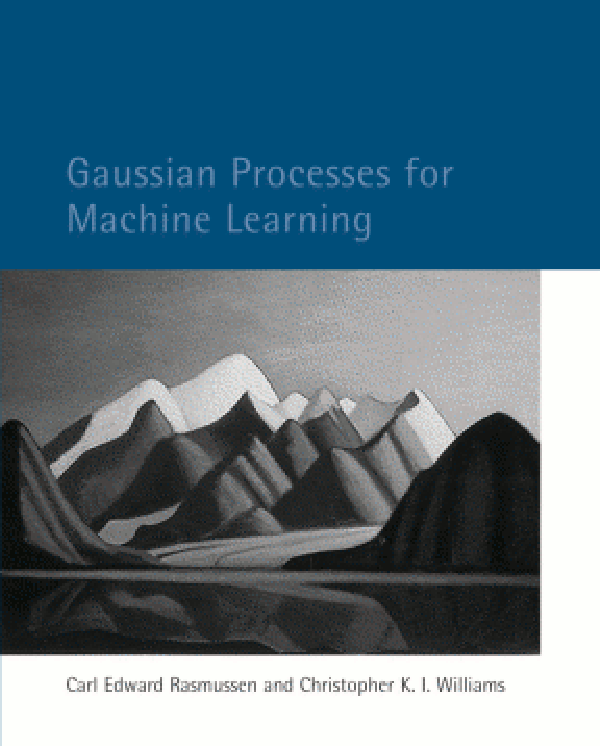
\includegraphics[scale=0.4]{figures/rwcover.pdf} \\
    \url{http://www.gaussianprocess.org/}
  \end{center}
  (Also code!)
\end{frame}

\begin{frame}{Regression}
  Consider the general \emphr{regression} problem.  Here we have:

  \begin{itemize}
    \item an input domain $\mc{X}$ (for example, $\R^n$, but in
      general anything),
    \item an unknown function $f\colon \mc{X} \to \R$, and
    \item and (perhaps noisy) observations of the function: $\data =
      \bigl\{ (\vec{x}_i, y_i) \bigr\}$, where $y_i = f(\vec{x}_i) +
      \epsilon_i$.
  \end{itemize}

  Our goal is to \emphr{predict} the value of the function
  $f(\mat{X}_\ast)$ at some test locations $\mat{X}_\ast$.
\end{frame}

\begin{frame}{Gaussian processes}
  \begin{itemize}
  \item Gaussian processes take a \emphr{nonparameteric} approach to
    regression.  We select a \emphr{prior distribution} over the
    function $f$ and condition this distribution on our observations,
    using the posterior distribution to make predictions.
  \item Gaussian processes are very \emphr{powerful} and leverage
    the many \emphr{convenient properties} of the Gaussian
    distribution to enable tractable inference.
  \end{itemize}
\end{frame}

\subsection{GPs: Prior}

\begin{frame}{From the Gaussian distribution to GPs}
  \begin{itemize}
    \item How can we leverage these useful properties of the Gaussian
      distribution to approach the regression problem?  We have a
      problem: the latent function $f$ is usually \emphr{infinite
        dimensional}; however, the multivariate Gaussian distribution
      is only useful in \emphr{finite dimensions.}
    \item The Gaussian process is a \emphr{natural generalization} of
      the multivariate Gaussian distribution to \emphr{potentially
        infinite settings.}
  \end{itemize}
\end{frame}

\begin{frame}{GPs: Definition}
  \begin{defn}[GPs]
    A \emphr{Gaussian process} is a (potentially infinite) collection
    of random variables such that the joint distribution of any finite
    number of them is multivariate Gaussian.
  \end{defn}
\end{frame}

\begin{frame}{GPs: Notation}
  A Gaussian process distribution on $f$ is written
  \begin{equation*}
    p(f) = \mc{GP}(f; \mu, K),
  \end{equation*}
  and just like the multivariate Gaussian distribution, is
  parameterized by its first two moments (now functions):
  \begin{itemize}
  \item $\Exp[f] = \mu\colon \mc{X} \to \R$, the \emphr{mean function,} and
  \item $\Exp\Bigl[\bigl(f(x) - \mu(x)\bigr)\bigl(f(x') - \mu(x')\bigr)\bigr]
    = K\colon \mc{X} \times \mc{X} \to \R$,
    a positive semidefinite \emphr{covariance function} or \emphr{kernel.}
  \end{itemize}
\end{frame}

\begin{frame}{GPs: Mean and covariance functions}
  \begin{itemize}
    \item The mean function encodes the \emphr{central tendency} of
      the function, and is often assumed to be a constant (usually
      zero).
    \item The covariance function encodes information about the
      \emphr{shape} and \emphr{structure} we expect the function to
      have.  A simple and very common example is the \emphr{squared
        exponential} covariance:
      \begin{equation*}
        K(\vec{x}, \vec{x}')
        =
        \exp\bigl(-\nicefrac{1}{2}\lVert \vec{x} - \vec{x}' \rVert^2\bigr),
      \end{equation*}
      which encodes the notation that ``nearby points should have
      similar function values.''
  \end{itemize}
\end{frame}

\begin{frame}{GPs: Prior on finite sets}
  Suppose we have selected a GP prior $\mc{GP}(f; \mu, K)$ for the
  function $f$.  Consider a finite set of points $\mat{X} \subseteq
  \mc{X}$.  The GP prior on $f$, by definition, \emphr{implies} the
  following joint distribution on the associated function values
  $\vec{f} = f(\mat{X})$:
  \begin{equation*}
    p(\vec{f} \given \mat{X})
    =
    \mc{N}(\vec{f}; \mu(\mat{X}), K(\mat{X}, \mat{X})\bigr).
  \end{equation*}
  That is, we simply evaluate the mean and covariance functions at $\mat{X}$
  and take the associated multivariate Gaussian distribution.  Very simple!
\end{frame}

\begin{frame}{Prior: Sampling examples}
  \hspace*{-1.5em}% This file was created by matlab2tikz.
% Minimal pgfplots version: 1.3
%
\tikzsetnextfilename{samples_example_1}
\definecolor{mycolor1}{rgb}{0.98824,0.57255,0.44706}%
\definecolor{mycolor2}{rgb}{0.98431,0.41569,0.29020}%
\definecolor{mycolor3}{rgb}{0.93725,0.23137,0.17255}%
\definecolor{mycolor4}{rgb}{0.65098,0.80784,0.89020}%
\definecolor{mycolor5}{rgb}{0.12157,0.47059,0.70588}%
%
\begin{tikzpicture}

\begin{axis}[%
width=0.95092\figurewidth,
height=\figureheight,
at={(0\figurewidth,0\figureheight)},
scale only axis,
xmin=0,
xmax=10,
xlabel={$x$},
ymin=-3,
ymax=3,
axis x line*=bottom,
axis y line*=left,
legend style={legend cell align=left,align=left,draw=white!15!black},
legend style={legend columns=-1, draw=none}, reverse legend
]
\addplot [color=mycolor1,solid,forget plot]
  table[row sep=crcr]{%
0	-0.356707751289252\\
0.01001001001001	-0.370042961505003\\
0.02002002002002	-0.383428680433551\\
0.03003003003003	-0.396860604294263\\
0.04004004004004	-0.410334475729796\\
0.0500500500500501	-0.423846086702714\\
0.0600600600600601	-0.437391281939299\\
0.0700700700700701	-0.450965963364064\\
0.0800800800800801	-0.464566091593718\\
0.0900900900900901	-0.478187692304172\\
0.1001001001001	-0.491826855863158\\
0.11011011011011	-0.505479743815741\\
0.12012012012012	-0.519142589596456\\
0.13013013013013	-0.532811701310166\\
0.14014014014014	-0.546483467137489\\
0.15015015015015	-0.560154354734848\\
0.16016016016016	-0.57382091633006\\
0.17017017017017	-0.587479789483759\\
0.18018018018018	-0.60112770002143\\
0.19019019019019	-0.614761465024442\\
0.2002002002002	-0.628377993098458\\
0.21021021021021	-0.641974288772261\\
0.22022022022022	-0.655547451837662\\
0.23023023023023	-0.66909468051711\\
0.24024024024024	-0.682613273234231\\
0.25025025025025	-0.696100628249111\\
0.26026026026026	-0.70955424757447\\
0.27027027027027	-0.722971736413654\\
0.28028028028028	-0.736350804728642\\
0.29029029029029	-0.749689267839638\\
0.3003003003003	-0.76298504807034\\
0.31031031031031	-0.776236174680745\\
0.32032032032032	-0.789440783835343\\
0.33033033033033	-0.802597121370997\\
0.34034034034034	-0.815703539654821\\
0.35035035035035	-0.828758500818559\\
0.36036036036036	-0.841760575359889\\
0.37037037037037	-0.85470844186264\\
0.38038038038038	-0.867600887215754\\
0.39039039039039	-0.880436806258112\\
0.4004004004004	-0.893215201041646\\
0.41041041041041	-0.90593518100492\\
0.42042042042042	-0.918595961056998\\
0.43043043043043	-0.931196861700559\\
0.44044044044044	-0.943737307239326\\
0.45045045045045	-0.956216825917655\\
0.46046046046046	-0.968635047181311\\
0.47047047047047	-0.980991701902679\\
0.48048048048048	-0.993286619936162\\
0.49049049049049	-1.00551972963598\\
0.500500500500501	-1.01769105443869\\
0.510510510510511	-1.02980071297867\\
0.520520520520521	-1.04184891682831\\
0.530530530530531	-1.05383596741236\\
0.540540540540541	-1.06576225656718\\
0.550550550550551	-1.07762826094085\\
0.560560560560561	-1.08943454305942\\
0.570570570570571	-1.1011817471379\\
0.580580580580581	-1.11287059728401\\
0.590590590590591	-1.12450189543097\\
0.600600600600601	-1.1360765179195\\
0.610610610610611	-1.14759541427313\\
0.620620620620621	-1.15905960266512\\
0.630630630630631	-1.17047016974792\\
0.640640640640641	-1.18182826517252\\
0.650650650650651	-1.19313510038869\\
0.660660660660661	-1.20439194611792\\
0.670670670670671	-1.21560012773666\\
0.680680680680681	-1.22676102371965\\
0.690690690690691	-1.23787606278924\\
0.700700700700701	-1.2489467182355\\
0.710710710710711	-1.25997450910981\\
0.720720720720721	-1.27096099275808\\
0.730730730730731	-1.28190776568388\\
0.740740740740741	-1.29281645610387\\
0.750750750750751	-1.30368872426206\\
0.760760760760761	-1.31452625805764\\
0.770770770770771	-1.32533076756353\\
0.780780780780781	-1.33610398590198\\
0.790790790790791	-1.34684766320365\\
0.800800800800801	-1.35756356261924\\
0.810810810810811	-1.36825345998258\\
0.820820820820821	-1.37891913765145\\
0.830830830830831	-1.38956238277605\\
0.840840840840841	-1.40018498315019\\
0.850850850850851	-1.41078872472715\\
0.860860860860861	-1.42137538811579\\
0.870870870870871	-1.43194674524203\\
0.880880880880881	-1.44250455539564\\
0.890890890890891	-1.45305056327183\\
0.900900900900901	-1.46358649444052\\
0.910910910910911	-1.47411405383092\\
0.920920920920921	-1.48463492186808\\
0.930930930930931	-1.49515075020397\\
0.940940940940941	-1.50566316048684\\
0.950950950950951	-1.51617374027425\\
0.960960960960961	-1.52668404066322\\
0.970970970970971	-1.53719557223126\\
0.980980980980981	-1.54770980455295\\
0.990990990990991	-1.55822816060295\\
1.001001001001	-1.56875201607183\\
1.01101101101101	-1.57928269425517\\
1.02102102102102	-1.589821467124\\
1.03103103103103	-1.60036954950907\\
1.04104104104104	-1.6109280969887\\
1.05105105105105	-1.62149820626017\\
1.06106106106106	-1.63208090766055\\
1.07107107107107	-1.64267716881978\\
1.08108108108108	-1.65328788710589\\
1.09109109109109	-1.66391389098738\\
1.1011011011011	-1.67455593666758\\
1.11111111111111	-1.68521470546659\\
1.12112112112112	-1.69589080298331\\
1.13113113113113	-1.70658475677354\\
1.14114114114114	-1.71729701539823\\
1.15115115115115	-1.72802794410645\\
1.16116116116116	-1.73877782676386\\
1.17117117117117	-1.74954686203778\\
1.18118118118118	-1.76033516275783\\
1.19119119119119	-1.77114275464956\\
1.2012012012012	-1.78196957471005\\
1.21121121121121	-1.79281547043606\\
1.22122122122122	-1.80368019798368\\
1.23123123123123	-1.81456342295279\\
1.24124124124124	-1.82546471718175\\
1.25125125125125	-1.83638356060067\\
1.26126126126126	-1.8473193377865\\
1.27127127127127	-1.8582713402475\\
1.28128128128128	-1.86923876260244\\
1.29129129129129	-1.88022070639199\\
1.3013013013013	-1.89121617588773\\
1.31131131131131	-1.90222408075171\\
1.32132132132132	-1.91324323350523\\
1.33133133133133	-1.92427235204171\\
1.34134134134134	-1.93531005803491\\
1.35135135135135	-1.94635487779478\\
1.36136136136136	-1.95740524249767\\
1.37137137137137	-1.96845948929387\\
1.38138138138138	-1.97951585967681\\
1.39139139139139	-1.9905725035717\\
1.4014014014014	-2.00162747687836\\
1.41141141141141	-2.01267874386191\\
1.42142142142142	-2.02372417862767\\
1.43143143143143	-2.03476156392144\\
1.44144144144144	-2.04578859485573\\
1.45145145145145	-2.05680287836839\\
1.46146146146146	-2.06780193660505\\
1.47147147147147	-2.07878320453719\\
1.48148148148148	-2.08974403616392\\
1.49149149149149	-2.10068170215031\\
1.5015015015015	-2.11159339476561\\
1.51151151151151	-2.12247622733823\\
1.52152152152152	-2.13332723664402\\
1.53153153153153	-2.14414338726771\\
1.54154154154154	-2.15492156851213\\
1.55155155155155	-2.1656586025714\\
1.56156156156156	-2.17635124277117\\
1.57157157157157	-2.1869961772217\\
1.58158158158158	-2.19759003110459\\
1.59159159159159	-2.20812936935259\\
1.6016016016016	-2.21861069939957\\
1.61161161161161	-2.22903047314376\\
1.62162162162162	-2.23938508996733\\
1.63163163163163	-2.24967090002152\\
1.64164164164164	-2.25988420732664\\
1.65165165165165	-2.27002127162375\\
1.66166166166166	-2.28007831112129\\
1.67167167167167	-2.29005150850499\\
1.68168168168168	-2.29993701081712\\
1.69169169169169	-2.30973093391033\\
1.7017017017017	-2.3194293659728\\
1.71171171171171	-2.32902837122671\\
1.72172172172172	-2.33852399192387\\
1.73173173173173	-2.34791225288754\\
1.74174174174174	-2.35718916475447\\
1.75175175175175	-2.36635072808142\\
1.76176176176176	-2.37539293563414\\
1.77177177177177	-2.38431177682276\\
1.78178178178178	-2.39310324135833\\
1.79179179179179	-2.4017633233815\\
1.8018018018018	-2.41028802420031\\
1.81181181181181	-2.41867335585548\\
1.82182182182182	-2.42691534676223\\
1.83183183183183	-2.43501004335235\\
1.84184184184184	-2.44295351517035\\
1.85185185185185	-2.45074185870631\\
1.86186186186186	-2.45837119959716\\
1.87187187187187	-2.46583769883944\\
1.88188188188188	-2.47313755509431\\
1.89189189189189	-2.48026700881739\\
1.9019019019019	-2.48722234582237\\
1.91191191191191	-2.49399990214239\\
1.92192192192192	-2.50059606625112\\
1.93193193193193	-2.50700728499184\\
1.94194194194194	-2.51323006433663\\
1.95195195195195	-2.5192609756215\\
1.96196196196196	-2.52509665878864\\
1.97197197197197	-2.53073382522603\\
1.98198198198198	-2.53616926179519\\
1.99199199199199	-2.54139983461587\\
2.002002002002	-2.54642249223129\\
2.01201201201201	-2.55123426940987\\
2.02202202202202	-2.5558322913907\\
2.03203203203203	-2.56021377424954\\
2.04204204204204	-2.56437603186435\\
2.05205205205205	-2.56831647757804\\
2.06206206206206	-2.57203262595111\\
2.07207207207207	-2.57552209866635\\
2.08208208208208	-2.57878262554644\\
2.09209209209209	-2.5818120477808\\
2.1021021021021	-2.5846083211063\\
2.11211211211211	-2.58716951811416\\
2.12212212212212	-2.5894938322836\\
2.13213213213213	-2.59157957828166\\
2.14214214214214	-2.59342519585177\\
2.15215215215215	-2.59502925145033\\
2.16216216216216	-2.59639044183269\\
2.17217217217217	-2.597507594005\\
2.18218218218218	-2.59837966944447\\
2.19219219219219	-2.59900576376174\\
2.2022022022022	-2.59938510990081\\
2.21221221221221	-2.59951708018687\\
2.22222222222222	-2.59940118595539\\
2.23223223223223	-2.59903708012874\\
2.24224224224224	-2.59842455873379\\
2.25225225225225	-2.5975635605101\\
2.26226226226226	-2.59645416997607\\
2.27227227227227	-2.59509661582306\\
2.28228228228228	-2.59349127386529\\
2.29229229229229	-2.59163866522604\\
2.3023023023023	-2.58953945907393\\
2.31231231231231	-2.58719447002692\\
2.32232232232232	-2.58460466133422\\
2.33233233233233	-2.58177114213477\\
2.34234234234234	-2.57869516826733\\
2.35235235235235	-2.57537814234467\\
2.36236236236236	-2.57182161200428\\
2.37237237237237	-2.5680272699418\\
2.38238238238238	-2.56399695305011\\
2.39239239239239	-2.55973264024517\\
2.4024024024024	-2.55523645329987\\
2.41241241241241	-2.55051065350563\\
2.42242242242242	-2.54555764108269\\
2.43243243243243	-2.54037995309227\\
2.44244244244244	-2.5349802623287\\
2.45245245245245	-2.52936137396406\\
2.46246246246246	-2.5235262254588\\
2.47247247247247	-2.51747788220612\\
2.48248248248248	-2.51121953553261\\
2.49249249249249	-2.50475450174881\\
2.5025025025025	-2.49808621654942\\
2.51251251251251	-2.49121823540091\\
2.52252252252252	-2.4841542277248\\
2.53253253253253	-2.47689797510144\\
2.54254254254254	-2.46945336746275\\
2.55255255255255	-2.4618244010854\\
2.56256256256256	-2.45401517232918\\
2.57257257257257	-2.44602987655627\\
2.58258258258258	-2.4378728027615\\
2.59259259259259	-2.42954833068931\\
2.6026026026026	-2.42106092635233\\
2.61261261261261	-2.4124151376852\\
2.62262262262262	-2.40361558998249\\
2.63263263263263	-2.39466698326521\\
2.64264264264264	-2.38557408605669\\
2.65265265265265	-2.37634173203502\\
2.66266266266266	-2.36697481422066\\
2.67267267267267	-2.35747828207181\\
2.68268268268268	-2.34785713491606\\
2.69269269269269	-2.33811641896552\\
2.7027027027027	-2.32826122062851\\
2.71271271271271	-2.31829666325972\\
2.72272272272272	-2.30822790095517\\
2.73273273273273	-2.29806011474398\\
2.74274274274274	-2.2877985064238\\
2.75275275275275	-2.27744829407865\\
2.76276276276276	-2.26701470758832\\
2.77277277277277	-2.25650298161042\\
2.78278278278278	-2.24591835305925\\
2.79279279279279	-2.23526605414151\\
2.8028028028028	-2.22455130854304\\
2.81281281281281	-2.21377932491344\\
2.82282282282282	-2.20295529245262\\
2.83283283283283	-2.19208437773843\\
2.84284284284284	-2.18117171528455\\
2.85285285285285	-2.17022240763039\\
2.86286286286286	-2.15924151665486\\
2.87287287287287	-2.14823406147711\\
2.88288288288288	-2.13720501054663\\
2.89289289289289	-2.12615927956196\\
2.9029029029029	-2.11510172657107\\
2.91291291291291	-2.10403714524423\\
2.92292292292292	-2.09297026190763\\
2.93293293293293	-2.08190573178912\\
2.94294294294294	-2.07084813301585\\
2.95295295295295	-2.0598019635048\\
2.96296296296296	-2.04877163605725\\
2.97297297297297	-2.03776147432296\\
2.98298298298298	-2.02677571076604\\
2.99299299299299	-2.01581847885818\\
3.003003003003	-2.00489381377367\\
3.01301301301301	-1.99400564549036\\
3.02302302302302	-1.98315779786208\\
3.03303303303303	-1.9723539834063\\
3.04304304304304	-1.96159780032349\\
3.05305305305305	-1.95089273148108\\
3.06306306306306	-1.94024213863446\\
3.07307307307307	-1.92964926163084\\
3.08308308308308	-1.91911721567818\\
3.09309309309309	-1.90864898810131\\
3.1031031031031	-1.89824743635864\\
3.11311311311311	-1.88791528679629\\
3.12312312312312	-1.87765513182319\\
3.13313313313313	-1.8674694280501\\
3.14314314314314	-1.85736049533829\\
3.15315315315315	-1.84733051455024\\
3.16316316316316	-1.83738152733685\\
3.17317317317317	-1.82751543407222\\
3.18318318318318	-1.81773399326599\\
3.19319319319319	-1.80803882103112\\
3.2032032032032	-1.79843139030511\\
3.21321321321321	-1.78891303018373\\
3.22322322322322	-1.7794849260914\\
3.23323323323323	-1.77014811971577\\
3.24324324324324	-1.76090350852359\\
3.25325325325325	-1.7517518466841\\
3.26326326326326	-1.74269374485668\\
3.27327327327327	-1.7337296719042\\
3.28328328328328	-1.72485995416032\\
3.29329329329329	-1.71608477729274\\
3.3033033033033	-1.70740418741818\\
3.31331331331331	-1.6988180912583\\
3.32332332332332	-1.69032625959027\\
3.33333333333333	-1.68192832593355\\
3.34334334334334	-1.67362379164284\\
3.35335335335335	-1.66541202438878\\
3.36336336336336	-1.65729226205657\\
3.37337337337337	-1.64926361483975\\
3.38338338338338	-1.64132506614522\\
3.39339339339339	-1.63347547713614\\
3.4034034034034	-1.62571358710008\\
3.41341341341341	-1.61803801627441\\
3.42342342342342	-1.61044727063346\\
3.43343343343343	-1.60293974204657\\
3.44344344344344	-1.59551371320609\\
3.45345345345345	-1.58816735961467\\
3.46346346346346	-1.58089875287886\\
3.47347347347347	-1.5737058641831\\
3.48348348348348	-1.56658656795244\\
3.49349349349349	-1.55953864344122\\
3.5035035035035	-1.55255978095343\\
3.51351351351351	-1.54564758367532\\
3.52352352352352	-1.53879957081319\\
3.53353353353353	-1.53201318301088\\
3.54354354354354	-1.52528578532085\\
3.55355355355355	-1.51861466925483\\
3.56356356356356	-1.51199705969778\\
3.57357357357357	-1.50543011672934\\
3.58358358358358	-1.49891094029007\\
3.59359359359359	-1.49243657301136\\
3.6036036036036	-1.48600400553054\\
3.61361361361361	-1.4796101804498\\
3.62362362362362	-1.47325199486237\\
3.63363363363363	-1.46692630659283\\
3.64364364364364	-1.46062993549644\\
3.65365365365365	-1.45435966962937\\
3.66366366366366	-1.4481122682596\\
3.67367367367367	-1.44188446692166\\
3.68368368368368	-1.43567297902504\\
3.69369369369369	-1.42947450293786\\
3.7037037037037	-1.42328572300307\\
3.71371371371371	-1.41710331550462\\
3.72372372372372	-1.41092395223734\\
3.73373373373373	-1.4047443026497\\
3.74374374374374	-1.39856104003269\\
3.75375375375375	-1.39237084307163\\
3.76376376376376	-1.38617040113196\\
3.77377377377377	-1.37995641847852\\
3.78378378378378	-1.37372561466789\\
3.79379379379379	-1.3674747313613\\
3.8038038038038	-1.36120053467425\\
3.81381381381381	-1.35489981900626\\
3.82382382382382	-1.34856940828873\\
3.83383383383383	-1.3422061631222\\
3.84384384384384	-1.33580698039948\\
3.85385385385385	-1.32936879759016\\
3.86386386386386	-1.32288859754564\\
3.87387387387387	-1.31636340828036\\
3.88388388388388	-1.30979030929145\\
3.89389389389389	-1.30316643162674\\
3.9039039039039	-1.29648896265538\\
3.91391391391391	-1.28975514634536\\
3.92392392392392	-1.28296228890207\\
3.93393393393393	-1.2761077591718\\
3.94394394394394	-1.2691889912656\\
3.95395395395395	-1.26220348765578\\
3.96396396396396	-1.25514882098283\\
3.97397397397397	-1.24802263661692\\
3.98398398398398	-1.24082265319823\\
3.99399399399399	-1.23354666678778\\
4.004004004004	-1.22619255220679\\
4.01401401401401	-1.21875826309265\\
4.02402402402402	-1.21124183633197\\
4.03403403403403	-1.20364139110378\\
4.04404404404404	-1.19595513295354\\
4.05405405405405	-1.18818135300499\\
4.06406406406406	-1.18031843143811\\
4.07407407407407	-1.17236483633626\\
4.08408408408408	-1.1643191282702\\
4.09409409409409	-1.1561799577616\\
4.1041041041041	-1.14794606892603\\
4.11411411411411	-1.13961629930685\\
4.12412412412412	-1.13118958187833\\
4.13413413413413	-1.12266494426352\\
4.14414414414414	-1.11404151093959\\
4.15415415415415	-1.10531850389225\\
4.16416416416416	-1.09649524078032\\
4.17417417417417	-1.08757113979056\\
4.18418418418418	-1.07854571724933\\
4.19419419419419	-1.06941858746203\\
4.2042042042042	-1.06018946470475\\
4.21421421421421	-1.05085816400815\\
4.22422422422422	-1.04142459883895\\
4.23423423423423	-1.03188878371909\\
4.24424424424424	-1.02225083342225\\
4.25425425425425	-1.01251096261431\\
4.26426426426426	-1.00266948592381\\
4.27427427427427	-0.992726819241655\\
4.28428428428428	-0.982683478035733\\
4.29429429429429	-0.972540077095034\\
4.3043043043043	-0.96229733136553\\
4.31431431431431	-0.951956055747436\\
4.32432432432432	-0.941517162931745\\
4.33433433433433	-0.930981665366503\\
4.34434434434434	-0.920350672995536\\
4.35435435435435	-0.909625394883566\\
4.36436436436436	-0.898807136177351\\
4.37437437437437	-0.887897298007659\\
4.38438438438438	-0.876897379827498\\
4.39439439439439	-0.865808975860552\\
4.4044044044044	-0.85463377353217\\
4.41441441441441	-0.843373556369914\\
4.42442442442442	-0.832030200388548\\
4.43443443443443	-0.820605674104022\\
4.44444444444444	-0.809102037487369\\
4.45445445445445	-0.797521442414852\\
4.46446446446446	-0.785866129363336\\
4.47447447447447	-0.77413842831741\\
4.48448448448448	-0.762340757966936\\
4.49449449449449	-0.750475622567509\\
4.5045045045045	-0.738545612489424\\
4.51451451451451	-0.726553404479488\\
4.52452452452452	-0.714501756823946\\
4.53453453453453	-0.702393511152497\\
4.54454454454454	-0.690231590951727\\
4.55455455455455	-0.678018998290946\\
4.56456456456456	-0.665758814771413\\
4.57457457457457	-0.653454200855695\\
4.58458458458458	-0.641108389569753\\
4.59459459459459	-0.628724691568717\\
4.6046046046046	-0.616306490148958\\
4.61461461461461	-0.603857238592243\\
4.62462462462462	-0.591380462989789\\
4.63463463463463	-0.578879755850426\\
4.64464464464464	-0.566358778704153\\
4.65465465465465	-0.553821256611609\\
4.66466466466466	-0.541270979946076\\
4.67467467467467	-0.528711799854327\\
4.68468468468468	-0.516147628759237\\
4.69469469469469	-0.503582437457165\\
4.7047047047047	-0.491020252792668\\
4.71471471471471	-0.478465156342855\\
4.72472472472472	-0.465921283358268\\
4.73473473473473	-0.453392819448612\\
4.74474474474474	-0.44088399856256\\
4.75475475475475	-0.428399102745113\\
4.76476476476476	-0.415942457160913\\
4.77477477477477	-0.40351843065958\\
4.78478478478478	-0.391131431429374\\
4.79479479479479	-0.378785906564218\\
4.8048048048048	-0.366486338939128\\
4.81481481481481	-0.35423724406316\\
4.82482482482482	-0.342043168745632\\
4.83483483483483	-0.329908689812268\\
4.84484484484484	-0.317838407366967\\
4.85485485485485	-0.305836948274148\\
4.86486486486486	-0.293908958560969\\
4.87487487487487	-0.282059103986257\\
4.88488488488488	-0.270292064279372\\
4.89489489489489	-0.25861253408095\\
4.9049049049049	-0.247025217902955\\
4.91491491491491	-0.235534827060806\\
4.92492492492492	-0.224146078812898\\
4.93493493493493	-0.212863691960692\\
4.94494494494494	-0.201692383800837\\
4.95495495495495	-0.19063686882072\\
4.96496496496496	-0.179701853014284\\
4.97497497497497	-0.168892033657563\\
4.98498498498498	-0.158212095673772\\
4.99499499499499	-0.147666706513192\\
5.00500500500501	-0.137260514879639\\
5.01501501501502	-0.126998147463549\\
5.02502502502503	-0.116884206522886\\
5.03503503503504	-0.106923263407479\\
5.04504504504505	-0.097119859931821\\
5.05505505505506	-0.0874785019747294\\
5.06506506506507	-0.07800365667218\\
5.07507507507508	-0.0686997507515888\\
5.08508508508509	-0.0595711643838633\\
5.0950950950951	-0.050622231989006\\
5.10510510510511	-0.0418572343613255\\
5.11511511511512	-0.0332803991806635\\
5.12512512512513	-0.0248958956302975\\
5.13513513513514	-0.0167078309934486\\
5.14514514514515	-0.00872024969707665\\
5.15515515515516	-0.00093712631911706\\
5.16516516516517	0.00663763375684993\\
5.17517517517518	0.0140002012450929\\
5.18518518518519	0.0211468233411162\\
5.1951951951952	0.0280738283162865\\
5.20520520520521	0.0347776280862014\\
5.21521521521522	0.0412547221730852\\
5.22522522522523	0.0475017005688291\\
5.23523523523524	0.0535152458844047\\
5.24524524524525	0.0592921380579634\\
5.25525525525526	0.0648292552241461\\
5.26526526526527	0.0701235788974823\\
5.27527527527528	0.0751721957483529\\
5.28528528528529	0.0799723002769107\\
5.2952952952953	0.0845211982096429\\
5.30530530530531	0.0888163082585092\\
5.31531531531532	0.0928551664927888\\
5.32532532532533	0.0966354275589964\\
5.33533533533534	0.10015486742719\\
5.34534534534535	0.103411385455555\\
5.35535535535536	0.106403008735757\\
5.36536536536537	0.109127891427854\\
5.37537537537538	0.111584319054982\\
5.38538538538539	0.113770709553494\\
5.3953953953954	0.11568561745457\\
5.40540540540541	0.117327731616362\\
5.41541541541542	0.118695880827481\\
5.42542542542543	0.119789033808804\\
5.43543543543544	0.120606301811328\\
5.44544544544545	0.121146938106427\\
5.45545545545546	0.12141034221569\\
5.46546546546547	0.121396057834254\\
5.47547547547548	0.121103777786723\\
5.48548548548549	0.120533341671397\\
5.4954954954955	0.119684738209664\\
5.50550550550551	0.118558105985821\\
5.51551551551552	0.117153734872634\\
5.52552552552553	0.115472063523851\\
5.53553553553554	0.11351368437918\\
5.54554554554555	0.111279339121755\\
5.55555555555556	0.108769922483369\\
5.56556556556557	0.105986480414003\\
5.57557557557558	0.102930209538865\\
5.58558558558559	0.0996024582413316\\
5.5955955955956	0.0960047253203122\\
5.60560560560561	0.0921386594667449\\
5.61561561561562	0.0880060582642681\\
5.62562562562563	0.0836088679236139\\
5.63563563563564	0.078949182783466\\
5.64564564564565	0.0740292416302074\\
5.65565565565566	0.0688514295311896\\
5.66566566566567	0.0634182739238634\\
5.67567567567568	0.0577324448953494\\
5.68568568568569	0.0517967515736401\\
5.6956956956957	0.0456141424536826\\
5.70570570570571	0.0391877006798141\\
5.71571571571572	0.0325206450671049\\
5.72572572572573	0.025616325125648\\
5.73573573573574	0.0184782194000982\\
5.74574574574575	0.011109933810823\\
5.75575575575576	0.00351519874301727\\
5.76576576576577	-0.00430213567095924\\
5.77577577577578	-0.0123380995989742\\
5.78578578578579	-0.0205886083339015\\
5.7957957957958	-0.0290494652036077\\
5.80580580580581	-0.037716364615964\\
5.81581581581582	-0.0465848957219833\\
5.82582582582583	-0.0556505458989271\\
5.83583583583584	-0.0649087034911705\\
5.84584584584585	-0.0743546628697897\\
5.85585585585586	-0.083983628105534\\
5.86586586586587	-0.093790715536223\\
5.87587587587588	-0.10377095875814\\
5.88588588588589	-0.113919313618259\\
5.8958958958959	-0.124230660216678\\
5.90590590590591	-0.134699808956636\\
5.91591591591592	-0.145321504220517\\
5.92592592592593	-0.156090428724123\\
5.93593593593594	-0.167001207763795\\
5.94594594594595	-0.1780484143385\\
5.95595595595596	-0.189226573429695\\
5.96596596596597	-0.200530166098587\\
5.97597597597598	-0.211953634596406\\
5.98598598598599	-0.22349138761632\\
5.995995995996	-0.235137804057981\\
6.00600600600601	-0.24688723839048\\
6.01601601601602	-0.258734025196713\\
6.02602602602603	-0.27067248323177\\
6.03603603603604	-0.282696921601692\\
6.04604604604605	-0.294801644515833\\
6.05605605605606	-0.306980954143067\\
6.06606606606607	-0.319229157900798\\
6.07607607607608	-0.331540570787884\\
6.08608608608609	-0.343909523169227\\
6.0960960960961	-0.356330362296928\\
6.10610610610611	-0.368797459172536\\
6.11611611611612	-0.381305212366705\\
6.12612612612613	-0.39384805323775\\
6.13613613613614	-0.40642044983515\\
6.14614614614615	-0.4190169109511\\
6.15615615615616	-0.43163199315907\\
6.16616616616617	-0.444260301825361\\
6.17617617617618	-0.456896497807462\\
6.18618618618619	-0.469535301044763\\
6.1961961961962	-0.482171494981835\\
6.20620620620621	-0.494799929191858\\
6.21621621621622	-0.50741552641499\\
6.22622622622623	-0.520013283626705\\
6.23623623623624	-0.532588277097518\\
6.24624624624625	-0.545135666420861\\
6.25625625625626	-0.557650697588289\\
6.26626626626627	-0.570128706803953\\
6.27627627627628	-0.582565124309892\\
6.28628628628629	-0.594955475497006\\
6.2962962962963	-0.607295387919278\\
6.30630630630631	-0.61958059080342\\
6.31631631631632	-0.631806919874883\\
6.32632632632633	-0.643970319522138\\
6.33633633633634	-0.656066845517524\\
6.34634634634635	-0.668092668420191\\
6.35635635635636	-0.680044073921511\\
6.36636636636637	-0.691917466569013\\
6.37637637637638	-0.703709372593248\\
6.38638638638639	-0.715416439810662\\
6.3963963963964	-0.727035440434347\\
6.40640640640641	-0.738563273618602\\
6.41641641641642	-0.74999696532506\\
6.42642642642643	-0.761333670618442\\
6.43643643643644	-0.772570674536629\\
6.44644644644645	-0.783705393068441\\
6.45645645645646	-0.794735374812472\\
6.46646646646647	-0.805658299502507\\
6.47647647647648	-0.816471981566981\\
6.48648648648649	-0.827174368300721\\
6.4964964964965	-0.837763541051569\\
6.50650650650651	-0.848237714444959\\
6.51651651651652	-0.858595237463152\\
6.52652652652653	-0.868834591666091\\
6.53653653653654	-0.878954393207182\\
6.54654654654655	-0.888953388207179\\
6.55655655655656	-0.898830457425256\\
6.56656656656657	-0.908584610594942\\
6.57657657657658	-0.918214987526118\\
6.58658658658659	-0.927720857325817\\
6.5965965965966	-0.937101615538947\\
6.60660660660661	-0.946356783729399\\
6.61661661661662	-0.955486008134962\\
6.62662662662663	-0.964489056663565\\
6.63663663663664	-0.973365818323377\\
6.64664664664665	-0.982116299832105\\
6.65665665665666	-0.990740624967195\\
6.66666666666667	-0.999239030181274\\
6.67667667667668	-1.00761186496844\\
6.68668668668669	-1.01585958613205\\
6.6966966966967	-1.02398275755119\\
6.70670670670671	-1.03198204643032\\
6.71671671671672	-1.03985821960258\\
6.72672672672673	-1.04761214239184\\
6.73673673673674	-1.05524477371706\\
6.74674674674675	-1.06275716313486\\
6.75675675675676	-1.07015044878405\\
6.76676676676677	-1.07742585257696\\
6.77677677677678	-1.08458467625328\\
6.78678678678679	-1.0916283002117\\
6.7967967967968	-1.09855817726461\\
6.80680680680681	-1.10537582973453\\
6.81681681681682	-1.1120828462581\\
6.82682682682683	-1.1186808767919\\
6.83683683683684	-1.12517162968179\\
6.84684684684685	-1.13155686703412\\
6.85685685685686	-1.13783840087927\\
6.86686686686687	-1.14401808871704\\
6.87687687687688	-1.15009782963086\\
6.88688688688689	-1.15607956091144\\
6.8968968968969	-1.1619652523879\\
6.90690690690691	-1.1677569028946\\
6.91691691691692	-1.17345653600765\\
6.92692692692693	-1.17906619645737\\
6.93693693693694	-1.18458794420627\\
6.94694694694695	-1.19002385200037\\
6.95695695695696	-1.19537599985506\\
6.96696696696697	-1.20064647162692\\
6.97697697697698	-1.20583734980703\\
6.98698698698699	-1.21095071223643\\
6.996996996997	-1.21598862770593\\
7.00700700700701	-1.22095315147824\\
7.01701701701702	-1.22584632107863\\
7.02702702702703	-1.230670153183\\
7.03703703703704	-1.23542663771084\\
7.04704704704705	-1.24011773610052\\
7.05705705705706	-1.24474537588107\\
7.06706706706707	-1.24931144614599\\
7.07707707707708	-1.25381779660647\\
7.08708708708709	-1.25826623025884\\
7.0970970970971	-1.26265850276293\\
7.10710710710711	-1.26699631603039\\
7.11711711711712	-1.27128131786691\\
7.12712712712713	-1.27551509549619\\
7.13713713713714	-1.27969917465715\\
7.14714714714715	-1.28383501429992\\
7.15715715715716	-1.28792400532753\\
7.16716716716717	-1.29196746613678\\
7.17717717717718	-1.29596664022626\\
7.18718718718719	-1.29992269409547\\
7.1971971971972	-1.30383671283792\\
7.20720720720721	-1.30770969919247\\
7.21721721721722	-1.31154256959218\\
7.22722722722723	-1.31533615406207\\
7.23723723723724	-1.31909119086006\\
7.24724724724725	-1.32280832776362\\
7.25725725725726	-1.32648811662194\\
7.26726726726727	-1.33013101431133\\
7.27727727727728	-1.33373737985266\\
7.28728728728729	-1.33730747342049\\
7.2972972972973	-1.3408414532785\\
7.30730730730731	-1.34433937688207\\
7.31731731731732	-1.34780119819085\\
7.32732732732733	-1.35122676679962\\
7.33733733733734	-1.35461582738567\\
7.34734734734735	-1.35796801889834\\
7.35735735735736	-1.36128287461763\\
7.36736736736737	-1.36455982003532\\
7.37737737737738	-1.36779817402987\\
7.38738738738739	-1.370997148912\\
7.3973973973974	-1.37415584962941\\
7.40740740740741	-1.37727327327039\\
7.41741741741742	-1.38034831251291\\
7.42742742742743	-1.383379751188\\
7.43743743743744	-1.3863662698951\\
7.44744744744745	-1.38930644326818\\
7.45745745745746	-1.39219874269384\\
7.46746746746747	-1.3950415361557\\
7.47747747747748	-1.39783309057324\\
7.48748748748749	-1.40057157212016\\
7.4974974974975	-1.40325504936248\\
7.50750750750751	-1.40588149171071\\
7.51751751751752	-1.40844877531222\\
7.52752752752753	-1.41095468174584\\
7.53753753753754	-1.41339690157747\\
7.54754754754755	-1.41577303524252\\
7.55755755755756	-1.41808059696835\\
7.56756756756757	-1.42031701676375\\
7.57757757757758	-1.42247964185921\\
7.58758758758759	-1.42456573969448\\
7.5975975975976	-1.42657250302662\\
7.60760760760761	-1.42849704940498\\
7.61761761761762	-1.43033642600095\\
7.62762762762763	-1.43208761257836\\
7.63763763763764	-1.43374752610904\\
7.64764764764765	-1.43531301906929\\
7.65765765765766	-1.4367808906244\\
7.66766766766767	-1.4381478831923\\
7.67767767767768	-1.4394106903396\\
7.68768768768769	-1.44056595860613\\
7.6976976976977	-1.44161029120478\\
7.70770770770771	-1.44254025328629\\
7.71771771771772	-1.44335237473453\\
7.72772772772773	-1.44404315504075\\
7.73773773773774	-1.44460906542883\\
7.74774774774775	-1.44504655633156\\
7.75775775775776	-1.44535205872087\\
7.76776776776777	-1.44552198932366\\
7.77777777777778	-1.4455527554628\\
7.78778778778779	-1.44544075980164\\
7.7977977977978	-1.44518240195153\\
7.80780780780781	-1.44477408655642\\
7.81781781781782	-1.44421222589327\\
7.82782782782783	-1.44349324442892\\
7.83783783783784	-1.4426135827703\\
7.84784784784785	-1.44156970470907\\
7.85785785785786	-1.44035809837062\\
7.86786786786787	-1.4389752834198\\
7.87787787787788	-1.43741781425357\\
7.88788788788789	-1.43568228455621\\
7.8978978978979	-1.43376533239986\\
7.90790790790791	-1.43166364557537\\
7.91791791791792	-1.42937396370234\\
7.92792792792793	-1.42689308434537\\
7.93793793793794	-1.42421786757395\\
7.94794794794795	-1.42134524053852\\
7.95795795795796	-1.4182721991188\\
7.96796796796797	-1.41499581683414\\
7.97797797797798	-1.4115132462875\\
7.98798798798799	-1.40782172180797\\
7.997997997998	-1.40391856858028\\
8.00800800800801	-1.39980120167891\\
8.01801801801802	-1.39546713175645\\
8.02802802802803	-1.39091397307602\\
8.03803803803804	-1.38613943871112\\
8.04804804804805	-1.3811413535033\\
8.05805805805806	-1.37591765126326\\
8.06806806806807	-1.3704663814162\\
8.07807807807808	-1.36478571219593\\
8.08808808808809	-1.35887393386151\\
8.0980980980981	-1.35272946149829\\
8.10810810810811	-1.34635083786323\\
8.11811811811812	-1.33973673882828\\
8.12812812812813	-1.33288597425118\\
8.13813813813814	-1.32579749059515\\
8.14814814814815	-1.31847037480794\\
8.15815815815816	-1.31090385621659\\
8.16816816816817	-1.30309731050319\\
8.17817817817818	-1.29505025941457\\
8.18818818818819	-1.28676237538078\\
8.1981981981982	-1.2782334821801\\
8.20820820820821	-1.26946355682599\\
8.21821821821822	-1.26045273318252\\
8.22822822822823	-1.25120130136918\\
8.23823823823824	-1.24170970843204\\
8.24824824824825	-1.23197856388174\\
8.25825825825826	-1.22200863769688\\
8.26826826826827	-1.21180086101179\\
8.27827827827828	-1.20135632910552\\
8.28828828828829	-1.1906762992873\\
8.2982982982983	-1.17976219472596\\
8.30830830830831	-1.16861560195402\\
8.31831831831832	-1.15723827201689\\
8.32832832832833	-1.14563212276874\\
8.33833833833834	-1.13379923420746\\
8.34834834834835	-1.12174185257027\\
8.35835835835836	-1.10946238674106\\
8.36836836836837	-1.09696340938005\\
8.37837837837838	-1.08424765762614\\
8.38838838838839	-1.07131802486796\\
8.3983983983984	-1.058177571407\\
8.40840840840841	-1.04482951243144\\
8.41841841841842	-1.03127722231861\\
8.42842842842843	-1.01752423174903\\
8.43843843843844	-1.00357422453553\\
8.44844844844845	-0.989431037861103\\
8.45845845845846	-0.975098659522315\\
8.46846846846847	-0.960581224766853\\
8.47847847847848	-0.945883013690486\\
8.48848848848849	-0.931008450984956\\
8.4984984984985	-0.915962100894197\\
8.50850850850851	-0.900748665998046\\
8.51851851851852	-0.885372981425713\\
8.52852852852853	-0.869840014887617\\
8.53853853853854	-0.85415486200731\\
8.54854854854855	-0.838322743176584\\
8.55855855855856	-0.822348998450908\\
8.56856856856857	-0.806239087536828\\
8.57857857857858	-0.789998580262449\\
8.58858858858859	-0.773633158440483\\
8.5985985985986	-0.757148607970502\\
8.60860860860861	-0.740550816853698\\
8.61861861861862	-0.723845769679141\\
8.62862862862863	-0.707039541914084\\
8.63863863863864	-0.690138297812697\\
8.64864864864865	-0.673148285667854\\
8.65865865865866	-0.656075830581697\\
8.66866866866867	-0.638927331791747\\
8.67867867867868	-0.621709258991694\\
8.68868868868869	-0.604428143054073\\
8.6986986986987	-0.587090573711186\\
8.70870870870871	-0.569703195003131\\
8.71871871871872	-0.552272699846776\\
8.72872872872873	-0.534805822822871\\
8.73873873873874	-0.517309336829792\\
8.74874874874875	-0.499790045339322\\
8.75875875875876	-0.482254781295598\\
8.76876876876877	-0.46471039773005\\
8.77877877877878	-0.447163763220522\\
8.78878878878879	-0.429621756466461\\
8.7987987987988	-0.412091261595209\\
8.80880880880881	-0.39457916206613\\
8.81881881881882	-0.377092333668302\\
8.82882882882883	-0.359637642374158\\
8.83883883883884	-0.342221934985181\\
8.84884884884885	-0.324852036737184\\
8.85885885885886	-0.307534740291767\\
8.86886886886887	-0.29027681057343\\
8.87887887887888	-0.273084964959547\\
8.88888888888889	-0.255965883972388\\
8.8988988988989	-0.238926191257963\\
8.90890890890891	-0.221972456251482\\
8.91891891891892	-0.205111189113475\\
8.92892892892893	-0.188348829362607\\
8.93893893893894	-0.171691748916512\\
8.94894894894895	-0.155146239591913\\
8.95895895895896	-0.138718512177032\\
8.96896896896897	-0.122414690136959\\
8.97897897897898	-0.106240805112469\\
8.98898898898899	-0.0902027906281859\\
8.998998998999	-0.0743064806973816\\
9.00900900900901	-0.0585576009311922\\
9.01901901901902	-0.0429617661762677\\
9.02902902902903	-0.0275244778915076\\
9.03903903903904	-0.0122511145075461\\
9.04904904904905	0.00285306467752061\\
9.05905905905906	0.0177829332867869\\
9.06906906906907	0.0325334950025396\\
9.07907907907908	0.0470998874879031\\
9.08908908908909	0.0614773904607079\\
9.0990990990991	0.07566142462947\\
9.10910910910911	0.0896475581190194\\
9.11911911911912	0.103431510276187\\
9.12912912912913	0.117009149407967\\
9.13913913913914	0.130376502479091\\
9.14914914914915	0.143529754829413\\
9.15915915915916	0.156465252776789\\
9.16916916916917	0.169179504313485\\
9.17917917917918	0.18166918521806\\
9.18918918918919	0.193931140448981\\
9.1991991991992	0.205962382532001\\
9.20920920920921	0.217760098087226\\
9.21921921921922	0.229321644252175\\
9.22922922922923	0.240644556281834\\
9.23923923923924	0.251726544681204\\
9.24924924924925	0.262565494500049\\
9.25925925925926	0.273159474284747\\
9.26926926926927	0.28350672657155\\
9.27927927927928	0.293605675390796\\
9.28928928928929	0.303454924703755\\
9.2992992992993	0.313053258453587\\
9.30930930930931	0.322399640280198\\
9.31931931931932	0.331493212554232\\
9.32932932932933	0.340333300368709\\
9.33933933933934	0.348919403404385\\
9.34934934934935	0.357251202285009\\
9.35935935935936	0.365328555382665\\
9.36936936936937	0.373151495479142\\
9.37937937937938	0.38072023171691\\
9.38938938938939	0.388035144972295\\
9.3993993993994	0.395096789240498\\
9.40940940940941	0.401905890067993\\
9.41941941941942	0.408463337609859\\
9.42942942942943	0.414770193161087\\
9.43943943943944	0.420827676200873\\
9.44944944944945	0.426637172416929\\
9.45945945945946	0.432200222918768\\
9.46946946946947	0.437518528022984\\
9.47947947947948	0.442593939145674\\
9.48948948948949	0.447428458481778\\
9.4994994994995	0.452024234709495\\
9.50950950950951	0.456383562194537\\
9.51951951951952	0.4605088734796\\
9.52952952952953	0.464402739411414\\
9.53953953953954	0.468067861922008\\
9.54954954954955	0.47150707439954\\
9.55955955955956	0.474723334928812\\
9.56956956956957	0.477719722602391\\
9.57957957957958	0.480499432545475\\
9.58958958958959	0.483065775164395\\
9.5995995995996	0.485422167815331\\
9.60960960960961	0.487572131194047\\
9.61961961961962	0.489519288184946\\
9.62962962962963	0.491267355539979\\
9.63963963963964	0.492820138824573\\
9.64964964964965	0.494181531155379\\
9.65965965965966	0.495355505668299\\
9.66966966966967	0.496346112893453\\
9.67967967967968	0.497157471429163\\
9.68968968968969	0.49779376928162\\
9.6996996996997	0.498259253135797\\
9.70970970970971	0.498558227756298\\
9.71971971971972	0.498695047686944\\
9.72972972972973	0.498674114396258\\
9.73973973973974	0.498499869151948\\
9.74974974974975	0.498176790354067\\
9.75975975975976	0.497709387276237\\
9.76976976976977	0.497102193511224\\
9.77977977977978	0.496359764268385\\
9.78978978978979	0.495486670890475\\
9.7997997997998	0.49448749393863\\
9.80980980980981	0.49336682108953\\
9.81981981981982	0.492129238927981\\
9.82982982982983	0.490779331292313\\
9.83983983983984	0.489321671948674\\
9.84984984984985	0.487760820224191\\
9.85985985985986	0.486101318340136\\
9.86986986986987	0.484347682695225\\
9.87987987987988	0.482504402115706\\
9.88988988988989	0.480575934627778\\
9.8998998998999	0.478566699493361\\
9.90990990990991	0.47648107277645\\
9.91991991991992	0.474323387262061\\
9.92992992992993	0.47209792217168\\
9.93993993993994	0.469808905605181\\
9.94994994994995	0.467460510168682\\
9.95995995995996	0.465056833086888\\
9.96996996996997	0.46260192678467\\
9.97997997997998	0.460099746936997\\
9.98998998998999	0.457554198352168\\
10	0.454969101914374\\
};
\addplot [color=mycolor2,solid,forget plot]
  table[row sep=crcr]{%
0	0.735205803646842\\
0.01001001001001	0.741095337313144\\
0.02002002002002	0.746985474444168\\
0.03003003003003	0.752871688070385\\
0.04004004004004	0.758749429178734\\
0.0500500500500501	0.764614131911058\\
0.0600600600600601	0.770461219280191\\
0.0700700700700701	0.776286108277684\\
0.0800800800800801	0.782084215844557\\
0.0900900900900901	0.787850963894684\\
0.1001001001001	0.793581785653054\\
0.11011011011011	0.799272130564681\\
0.12012012012012	0.804917470693359\\
0.13013013013013	0.810513306210502\\
0.14014014014014	0.816055170769745\\
0.15015015015015	0.82153863791296\\
0.16016016016016	0.826959326214641\\
0.17017017017017	0.832312905459143\\
0.18018018018018	0.837595102260767\\
0.19019019019019	0.842801705459185\\
0.2002002002002	0.847928572362792\\
0.21021021021021	0.852971633663606\\
0.22022022022022	0.857926899651913\\
0.23023023023023	0.862790465423\\
0.24024024024024	0.867558516254612\\
0.25025025025025	0.872227333327599\\
0.26026026026026	0.876793298609631\\
0.27027027027027	0.881252900243479\\
0.28028028028028	0.885602737689249\\
0.29029029029029	0.889839526764083\\
0.3003003003003	0.893960104242285\\
0.31031031031031	0.897961432968014\\
0.32032032032032	0.901840606431915\\
0.33033033033033	0.905594852860874\\
0.34034034034034	0.90922154035523\\
0.35035035035035	0.912718180274048\\
0.36036036036036	0.916082431724568\\
0.37037037037037	0.919312105489342\\
0.38038038038038	0.922405167569716\\
0.39039039039039	0.925359742850808\\
0.4004004004004	0.928174118291332\\
0.41041041041041	0.930846746171654\\
0.42042042042042	0.93337624728109\\
0.43043043043043	0.9357614133496\\
0.44044044044044	0.938001209954507\\
0.45045045045045	0.940094778603481\\
0.46046046046046	0.942041439177839\\
0.47047047047047	0.943840691642139\\
0.48048048048048	0.945492217855181\\
0.49049049049049	0.946995882967687\\
0.500500500500501	0.948351737119779\\
0.510510510510511	0.949560015883102\\
0.520520520520521	0.950621141390429\\
0.530530530530531	0.951535723109864\\
0.540540540540541	0.952304557571218\\
0.550550550550551	0.952928629313019\\
0.560560560560561	0.953409109986958\\
0.570570570570571	0.953747358395584\\
0.580580580580581	0.953944919968249\\
0.590590590590591	0.954003525419505\\
0.600600600600601	0.953925090277493\\
0.610610610610611	0.953711713046781\\
0.620620620620621	0.953365674117451\\
0.630630630630631	0.952889433349792\\
0.640640640640641	0.952285628718368\\
0.650650650650651	0.951557073618003\\
0.660660660660661	0.950706754346117\\
0.670670670670671	0.949737827642956\\
0.680680680680681	0.948653617490842\\
0.690690690690691	0.947457611997161\\
0.700700700700701	0.946153460335627\\
0.710710710710711	0.944744968405211\\
0.720720720720721	0.943236095881133\\
0.730730730730731	0.941630951276027\\
0.740740740740741	0.939933788715546\\
0.750750750750751	0.938149002674431\\
0.760760760760761	0.93628112364023\\
0.770770770770771	0.934334813894017\\
0.780780780780781	0.932314861421217\\
0.790790790790791	0.930226175573677\\
0.800800800800801	0.928073781818267\\
0.810810810810811	0.925862815657314\\
0.820820820820821	0.923598517598789\\
0.830830830830831	0.92128622704884\\
0.840840840840841	0.918931376680477\\
0.850850850850851	0.916539486172859\\
0.860860860860861	0.914116156031761\\
0.870870870870871	0.911667061535134\\
0.880880880880881	0.909197946317707\\
0.890890890890891	0.906714615838911\\
0.900900900900901	0.904222930948419\\
0.910910910910911	0.901728800986438\\
0.920920920920921	0.899238177174737\\
0.930930930930931	0.896757046216475\\
0.940940940940941	0.894291422985698\\
0.950950950950951	0.891847343876458\\
0.960960960960961	0.889430859961404\\
0.970970970970971	0.88704802994928\\
0.980980980980981	0.884704913094419\\
0.990990990990991	0.882407562641823\\
1.001001001001	0.880162018454481\\
1.01101101101101	0.877974300597294\\
1.02102102102102	0.875850401618286\\
1.03103103103103	0.873796280310537\\
1.04104104104104	0.871817854740526\\
1.05105105105105	0.869920994929334\\
1.06106106106106	0.868111517029474\\
1.07107107107107	0.866395175449875\\
1.08108108108108	0.864777657261389\\
1.09109109109109	0.863264575040376\\
1.1011011011011	0.861861460442797\\
1.11111111111111	0.860573758207116\\
1.12112112112112	0.859406819379336\\
1.13113113113113	0.858365895565104\\
1.14114114114114	0.857456132394646\\
1.15115115115115	0.856682564459441\\
1.16116116116116	0.856050108529257\\
1.17117117117117	0.855563558568106\\
1.18118118118118	0.855227580028452\\
1.19119119119119	0.855046704424721\\
1.2012012012012	0.855025324370623\\
1.21121121121121	0.855167688385005\\
1.22122122122122	0.855477896226967\\
1.23123123123123	0.855959893893564\\
1.24124124124124	0.856617469626498\\
1.25125125125125	0.857454249027889\\
1.26126126126126	0.858473691607348\\
1.27127127127127	0.859679086258864\\
1.28128128128128	0.861073548163058\\
1.29129129129129	0.862660014565736\\
1.3013013013013	0.864441242259359\\
1.31131131131131	0.866419803769824\\
1.32132132132132	0.868598085270117\\
1.33133133133133	0.870978283238762\\
1.34134134134134	0.873562402295963\\
1.35135135135135	0.876352253197043\\
1.36136136136136	0.879349450534682\\
1.37137137137137	0.882555411056037\\
1.38138138138138	0.885971352451637\\
1.39139139139139	0.889598291452411\\
1.4014014014014	0.89343704327139\\
1.41141141141141	0.897488220580153\\
1.42142142142142	0.901752232689483\\
1.43143143143143	0.906229285536228\\
1.44144144144144	0.91091938119755\\
1.45145145145145	0.915822318052273\\
1.46146146146146	0.920937690833315\\
1.47147147147147	0.926264891724584\\
1.48148148148148	0.931803110277872\\
1.49149149149149	0.937551335070696\\
1.5015015015015	0.943508354155686\\
1.51151151151151	0.949672756995834\\
1.52152152152152	0.956042935852246\\
1.53153153153153	0.962617086965744\\
1.54154154154154	0.96939321382767\\
1.55155155155155	0.976369127898086\\
1.56156156156156	0.98354245188675\\
1.57157157157157	0.990910621930691\\
1.58158158158158	0.998470890481304\\
1.59159159159159	1.00622032897933\\
1.6016016016016	1.01415583107653\\
1.61161161161161	1.02227411598648\\
1.62162162162162	1.03057173171481\\
1.63163163163163	1.03904505864985\\
1.64164164164164	1.04769031320355\\
1.65165165165165	1.05650355190388\\
1.66166166166166	1.06548067537943\\
1.67167167167167	1.07461743199006\\
1.68168168168168	1.08390942272458\\
1.69169169169169	1.09335210532864\\
1.7017017017017	1.10294079865984\\
1.71171171171171	1.11267068734171\\
1.72172172172172	1.12253682679095\\
1.73173173173173	1.13253414756843\\
1.74174174174174	1.14265746047468\\
1.75175175175175	1.15290146140969\\
1.76176176176176	1.16326073654198\\
1.77177177177177	1.17372976742024\\
1.78178178178178	1.18430293595573\\
1.79179179179179	1.19497452966432\\
1.8018018018018	1.20573874712113\\
1.81181181181181	1.21658970319075\\
1.82182182182182	1.22752143408418\\
1.83183183183183	1.23852790315253\\
1.84184184184184	1.24960300588285\\
1.85185185185185	1.26074057541383\\
1.86186186186186	1.27193438820252\\
1.87187187187187	1.28317816890596\\
1.88188188188188	1.29446559611204\\
1.89189189189189	1.30579030756139\\
1.9019019019019	1.3171459057528\\
1.91191191191191	1.32852596277612\\
1.92192192192192	1.33992402613851\\
1.93193193193193	1.3513336234734\\
1.94194194194194	1.36274826839869\\
1.95195195195195	1.37416146512381\\
1.96196196196196	1.38556671366778\\
1.97197197197197	1.39695751508233\\
1.98198198198198	1.40832737636098\\
1.99199199199199	1.41966981529144\\
2.002002002002	1.43097836526796\\
2.01201201201201	1.44224658015966\\
2.02202202202202	1.4534680386966\\
2.03203203203203	1.46463634967907\\
2.04204204204204	1.47574515574453\\
2.05205205205205	1.48678813807341\\
2.06206206206206	1.49775902104411\\
2.07207207207207	1.50865157565094\\
2.08208208208208	1.5194596242552\\
2.09209209209209	1.53017704433508\\
2.1021021021021	1.5407977724238\\
2.11211211211211	1.55131580779318\\
2.12212212212212	1.56172521585826\\
2.13213213213213	1.57202013229772\\
2.14214214214214	1.58219476607604\\
2.15215215215215	1.59224340279986\\
2.16216216216216	1.6021604076782\\
2.17217217217217	1.61194022901978\\
2.18218218218218	1.62157740064239\\
2.19219219219219	1.6310665451825\\
2.2022022022022	1.64040237638976\\
2.21221221221221	1.6495797016052\\
2.22222222222222	1.65859342453707\\
2.23223223223223	1.66743854739079\\
2.24224224224224	1.67611017277511\\
2.25225225225225	1.68460350626746\\
2.26226226226226	1.69291385771077\\
2.27227227227227	1.70103664358955\\
2.28228228228228	1.70896738811579\\
2.29229229229229	1.71670172537275\\
2.3023023023023	1.72423540014005\\
2.31231231231231	1.73156426983053\\
2.32232232232232	1.73868430495723\\
2.33233233233233	1.74559159081033\\
2.34234234234234	1.75228232811665\\
2.35235235235235	1.75875283389335\\
2.36236236236236	1.76499954219816\\
2.37237237237237	1.77101900480116\\
2.38238238238238	1.77680789158639\\
2.39239239239239	1.78236299120116\\
2.4024024024024	1.78768121095137\\
2.41241241241241	1.79275957740276\\
2.42242242242242	1.7975952363107\\
2.43243243243243	1.80218545270818\\
2.44244244244244	1.80652761067797\\
2.45245245245245	1.81061921348998\\
2.46246246246246	1.81445788293907\\
2.47247247247247	1.81804135938706\\
2.48248248248248	1.82136750130249\\
2.49249249249249	1.82443428448626\\
2.5025025025025	1.82723980200309\\
2.51251251251251	1.82978226291214\\
2.52252252252252	1.83205999223618\\
2.53253253253253	1.83407142976898\\
2.54254254254254	1.83581512950918\\
2.55255255255255	1.83728975837816\\
2.56256256256256	1.83849409595757\\
2.57257257257257	1.83942703283205\\
2.58258258258258	1.84008756998122\\
2.59259259259259	1.84047481747171\\
2.6026026026026	1.84058799340425\\
2.61261261261261	1.84042642281826\\
2.62262262262262	1.83998953649187\\
2.63263263263263	1.83927686946883\\
2.64264264264264	1.83828806005084\\
2.65265265265265	1.83702284831494\\
2.66266266266266	1.83548107502508\\
2.67267267267267	1.83366267986606\\
2.68268268268268	1.83156770055189\\
2.69269269269269	1.82919627094901\\
2.7027027027027	1.82654862005469\\
2.71271271271271	1.82362507027644\\
2.72272272272272	1.8204260361872\\
2.73273273273273	1.8169520228111\\
2.74274274274274	1.81320362439514\\
2.75275275275275	1.809181522825\\
2.76276276276276	1.80488648603722\\
2.77277277277277	1.80031936680798\\
2.78278278278278	1.7954811008402\\
2.79279279279279	1.79037270556218\\
2.8028028028028	1.784995278419\\
2.81281281281281	1.7793499955483\\
2.82282282282282	1.77343811029582\\
2.83283283283283	1.76726095115099\\
2.84284284284284	1.76081992130424\\
2.85285285285285	1.75411649600163\\
2.86286286286286	1.74715222179014\\
2.87287287287287	1.73992871456496\\
2.88288288288288	1.73244765865658\\
2.89289289289289	1.72471080472857\\
2.9029029029029	1.71671996843526\\
2.91291291291291	1.70847702933514\\
2.92292292292292	1.69998392911228\\
2.93293293293293	1.6912426699456\\
2.94294294294294	1.68225531340963\\
2.95295295295295	1.67302397878825\\
2.96296296296296	1.66355084184516\\
2.97297297297297	1.65383813325018\\
2.98298298298298	1.64388813686279\\
2.99299299299299	1.6337031891889\\
3.003003003003	1.62328567690731\\
3.01301301301301	1.61263803627824\\
3.02302302302302	1.60176275115275\\
3.03303303303303	1.59066235207538\\
3.04304304304304	1.57933941472529\\
3.05305305305305	1.56779655820818\\
3.06306306306306	1.55603644432408\\
3.07307307307307	1.54406177573651\\
3.08308308308308	1.53187529465282\\
3.09309309309309	1.5194797816624\\
3.1031031031031	1.50687805434776\\
3.11311311311311	1.49407296576209\\
3.12312312312312	1.48106740323203\\
3.13313313313313	1.46786428711937\\
3.14314314314314	1.45446656934747\\
3.15315315315315	1.44087723219598\\
3.16316316316316	1.42709928681074\\
3.17317317317317	1.41313577216683\\
3.18318318318318	1.39898975354068\\
3.19319319319319	1.38466432131372\\
3.2032032032032	1.37016258965439\\
3.21321321321321	1.35548769527645\\
3.22322322322322	1.34064279613014\\
3.23323323323323	1.325631070056\\
3.24324324324324	1.31045571373816\\
3.25325325325325	1.29511994120336\\
3.26326326326326	1.27962698278232\\
3.27327327327327	1.26398008357472\\
3.28328328328328	1.24818250260736\\
3.29329329329329	1.2322375113282\\
3.3033033033033	1.21614839242602\\
3.31331331331331	1.19991843887193\\
3.32332332332332	1.18355095223674\\
3.33333333333333	1.16704924217131\\
3.34334334334334	1.15041662447939\\
3.35335335335335	1.1336564206923\\
3.36336336336336	1.11677195650015\\
3.37337337337337	1.09976656069101\\
3.38338338338338	1.08264356422384\\
3.39339339339339	1.06540629879828\\
3.4034034034034	1.04805809612349\\
3.41341341341341	1.0306022869836\\
3.42342342342342	1.01304219952453\\
3.43343343343343	0.995381159111659\\
3.44344344344344	0.977622486676538\\
3.45345345345345	0.959769498174367\\
3.46346346346346	0.941825503533427\\
3.47347347347347	0.923793805687436\\
3.48348348348348	0.90567769967781\\
3.49349349349349	0.887480472254389\\
3.5035035035035	0.869205400336865\\
3.51351351351351	0.850855750723322\\
3.52352352352352	0.832434779428193\\
3.53353353353353	0.813945730615012\\
3.54354354354354	0.79539183604824\\
3.55355355355355	0.776776314888073\\
3.56356356356356	0.758102372420286\\
3.57357357357357	0.739373199950838\\
3.58358358358358	0.720591974114827\\
3.59359359359359	0.701761856741096\\
3.6036036036036	0.682885993970734\\
3.61361361361361	0.663967516072334\\
3.62362362362362	0.64500953732708\\
3.63363363363363	0.626015155289139\\
3.64364364364364	0.606987451110612\\
3.65365365365365	0.587929488994589\\
3.66366366366366	0.568844316124698\\
3.67367367367367	0.549734962428335\\
3.68368368368368	0.530604441077636\\
3.69369369369369	0.511455747800913\\
3.7037037037037	0.492291861556674\\
3.71371371371371	0.473115744257016\\
3.72372372372372	0.453930340972013\\
3.73373373373373	0.434738580496306\\
3.74374374374374	0.415543375149546\\
3.75375375375375	0.396347621581783\\
3.76376376376376	0.377154200750132\\
3.77377377377377	0.357965978295301\\
3.78378378378378	0.338785805590078\\
3.79379379379379	0.319616519756158\\
3.8038038038038	0.300460944272782\\
3.81381381381381	0.281321889642044\\
3.82382382382382	0.262202154476183\\
3.83383383383383	0.243104525334021\\
3.84384384384384	0.224031778345662\\
3.85385385385385	0.204986679694718\\
3.86386386386386	0.185971986074101\\
3.87387387387387	0.16699044633354\\
3.88388388388388	0.148044801616128\\
3.89389389389389	0.129137786861165\\
3.9039039039039	0.110272131466109\\
3.91391391391391	0.0914505607444892\\
3.92392392392392	0.0726757962913134\\
3.93393393393393	0.0539505576681409\\
3.94394394394394	0.0352775632188777\\
3.95395395395395	0.0166595312701907\\
3.96396396396396	-0.0019008188155807\\
3.97397397397397	-0.0204007654875626\\
3.98398398398398	-0.0388375834572758\\
3.99399399399399	-0.0572085430475107\\
4.004004004004	-0.0755109089081711\\
4.01401401401401	-0.0937419383692225\\
4.02402402402402	-0.111898880801921\\
4.03403403403403	-0.129978975956845\\
4.04404404404404	-0.147979453289782\\
4.05405405405405	-0.165897530205883\\
4.06406406406406	-0.183730411440045\\
4.07407407407407	-0.201475287285368\\
4.08408408408408	-0.219129333260503\\
4.09409409409409	-0.236689708128716\\
4.1041041041041	-0.254153553412662\\
4.11411411411411	-0.271517992035552\\
4.12412412412412	-0.288780127550965\\
4.13413413413413	-0.305937042843334\\
4.14414414414414	-0.322985799438169\\
4.15415415415415	-0.339923436527086\\
4.16416416416416	-0.356746969739737\\
4.17417417417417	-0.373453391096699\\
4.18418418418418	-0.390039667738211\\
4.19419419419419	-0.406502741042189\\
4.2042042042042	-0.422839526373299\\
4.21421421421421	-0.439046912591731\\
4.22422422422422	-0.455121761046239\\
4.23423423423423	-0.471060905567648\\
4.24424424424424	-0.486861152007883\\
4.25425425425425	-0.50251927784507\\
4.26426426426426	-0.518032031917396\\
4.27427427427427	-0.533396134696481\\
4.28428428428428	-0.548608277851743\\
4.29429429429429	-0.563665124267603\\
4.3043043043043	-0.578563308457219\\
4.31431431431431	-0.593299436718062\\
4.32432432432432	-0.607870087179622\\
4.33433433433433	-0.622271810605622\\
4.34434434434434	-0.636501130542998\\
4.35435435435435	-0.650554544485286\\
4.36436436436436	-0.664428523849093\\
4.37437437437437	-0.678119515067997\\
4.38438438438438	-0.691623941045897\\
4.39439439439439	-0.704938201591807\\
4.4044044044044	-0.718058674339896\\
4.41441441441441	-0.730981716768597\\
4.42442442442442	-0.743703666925728\\
4.43443443443443	-0.756220845070932\\
4.44444444444444	-0.768529555146506\\
4.45445445445445	-0.780626086796564\\
4.46446446446446	-0.792506716529283\\
4.47447447447447	-0.804167710078898\\
4.48448448448448	-0.815605324343869\\
4.49449449449449	-0.826815809109729\\
4.5045045045045	-0.837795409489461\\
4.51451451451451	-0.848540368591147\\
4.52452452452452	-0.85904692906771\\
4.53453453453453	-0.869311336263564\\
4.54454454454454	-0.879329840723046\\
4.55455455455455	-0.889098700435239\\
4.56456456456456	-0.898614184201896\\
4.57457457457457	-0.907872574488919\\
4.58458458458458	-0.916870169382847\\
4.59459459459459	-0.9256032870901\\
4.6046046046046	-0.934068268202603\\
4.61461461461461	-0.942261478682367\\
4.62462462462462	-0.95017931413227\\
4.63463463463463	-0.957818201981731\\
4.64464464464464	-0.965174606007473\\
4.65465465465465	-0.972245028724878\\
4.66466466466466	-0.979026015975505\\
4.67467467467467	-0.985514159751876\\
4.68468468468468	-0.991706102325651\\
4.69469469469469	-0.997598539882239\\
4.7047047047047	-1.0031882259608\\
4.71471471471471	-1.00847197556578\\
4.72472472472472	-1.01344666912056\\
4.73473473473473	-1.01810925594878\\
4.74474474474474	-1.02245675826632\\
4.75475475475475	-1.02648627552857\\
4.76476476476476	-1.03019498756436\\
4.77477477477477	-1.03358015928084\\
4.78478478478478	-1.03663914399449\\
4.79479479479479	-1.03936938788836\\
4.8048048048048	-1.04176843367128\\
4.81481481481481	-1.04383392437941\\
4.82482482482482	-1.04556360747494\\
4.83483483483483	-1.04695533908594\\
4.84484484484484	-1.04800708673028\\
4.85485485485485	-1.0487169347293\\
4.86486486486486	-1.04908308666365\\
4.87487487487487	-1.04910386996918\\
4.88488488488488	-1.04877773879791\\
4.89489489489489	-1.04810327871059\\
4.9049049049049	-1.04707920949952\\
4.91491491491491	-1.04570438877514\\
4.92492492492492	-1.04397781584034\\
4.93493493493493	-1.0418986347971\\
4.94494494494494	-1.0394661375949\\
4.95495495495495	-1.03667976787374\\
4.96496496496496	-1.03353912325032\\
4.97497497497497	-1.03004395911973\\
4.98498498498498	-1.02619419144006\\
4.99499499499499	-1.02198989896989\\
5.00500500500501	-1.01743132649712\\
5.01501501501502	-1.0125188874083\\
5.02502502502503	-1.00725316627618\\
5.03503503503504	-1.00163492048736\\
5.04504504504505	-0.995665083573163\\
5.05505505505506	-0.989344766474679\\
5.06506506506507	-0.982675259681059\\
5.07507507507508	-0.975658035399623\\
5.08508508508509	-0.968294748544408\\
5.0950950950951	-0.960587239289538\\
5.10510510510511	-0.952537533293945\\
5.11511511511512	-0.944147843911326\\
5.12512512512513	-0.935420572718331\\
5.13513513513514	-0.926358310425351\\
5.14514514514515	-0.91696383825125\\
5.15515515515516	-0.90724012751167\\
5.16516516516517	-0.89719034111126\\
5.17517517517518	-0.886817832894864\\
5.18518518518519	-0.876126148402696\\
5.1951951951952	-0.865119024529859\\
5.20520520520521	-0.853800389367865\\
5.21521521521522	-0.842174361672454\\
5.22522522522523	-0.830245250275745\\
5.23523523523524	-0.818017553587847\\
5.24524524524525	-0.805495958230025\\
5.25525525525526	-0.792685338528333\\
5.26526526526527	-0.779590754582838\\
5.27527527527528	-0.76621745115468\\
5.28528528528529	-0.752570856024582\\
5.2952952952953	-0.73865657810315\\
5.30530530530531	-0.724480405657845\\
5.31531531531532	-0.710048303702134\\
5.32532532532533	-0.695366412084898\\
5.33533533533534	-0.680441042869661\\
5.34534534534535	-0.665278677848022\\
5.35535535535536	-0.649885965117374\\
5.36536536536537	-0.634269716909515\\
5.37537537537538	-0.618436905845432\\
5.38538538538539	-0.602394661928075\\
5.3953953953954	-0.586150268486751\\
5.40540540540541	-0.569711159606019\\
5.41541541541542	-0.553084915396763\\
5.42542542542543	-0.536279258475928\\
5.43543543543544	-0.519302049619376\\
5.44544544544545	-0.502161284094818\\
5.45545545545546	-0.484865086519892\\
5.46546546546547	-0.467421707219928\\
5.47547547547548	-0.44983951665996\\
5.48548548548549	-0.432127001483108\\
5.4954954954955	-0.414292759324397\\
5.50550550550551	-0.396345493758928\\
5.51551551551552	-0.378294009013809\\
5.52552552552553	-0.360147205490039\\
5.53553553553554	-0.341914073250007\\
5.54554554554555	-0.323603687826629\\
5.55555555555556	-0.305225203695085\\
5.56556556556557	-0.286787849173887\\
5.57557557557558	-0.268300920739387\\
5.58558558558559	-0.249773776942893\\
5.5955955955956	-0.231215832747569\\
5.60560560560561	-0.212636553560393\\
5.61561561561562	-0.194045449340236\\
5.62562562562563	-0.17545206833056\\
5.63563563563564	-0.156865990870509\\
5.64564564564565	-0.138296823841872\\
5.65565565565566	-0.119754193693807\\
5.66566566566567	-0.101247740812663\\
5.67567567567568	-0.0827871127969811\\
5.68568568568569	-0.0643819586525399\\
5.6956956956957	-0.0460419219083992\\
5.70570570570571	-0.0277766349974405\\
5.71571571571572	-0.00959571213847105\\
5.72572572572573	0.00849125633115774\\
5.73573573573574	0.0264747104380645\\
5.74574574574575	0.0443451271111651\\
5.75575575575576	0.0620930264298982\\
5.76576576576577	0.0797089773820829\\
5.77577577577578	0.0971836048369716\\
5.78578578578579	0.114507595289923\\
5.7957957957958	0.131671703096069\\
5.80580580580581	0.148666756646174\\
5.81581581581582	0.165483664322415\\
5.82582582582583	0.182113420551117\\
5.83583583583584	0.198547111932743\\
5.84584584584585	0.214775922753256\\
5.85585585585586	0.2307911408397\\
5.86586586586587	0.246584163580762\\
5.87587587587588	0.262146503311498\\
5.88588588588589	0.277469792606179\\
5.8958958958959	0.292545790262279\\
5.90590590590591	0.307366386163878\\
5.91591591591592	0.321923606675525\\
5.92592592592593	0.336209619764468\\
5.93593593593594	0.350216740036525\\
5.94594594594595	0.363937433457855\\
5.95595595595596	0.377364322162864\\
5.96596596596597	0.390490189230866\\
5.97597597597598	0.403307983009882\\
5.98598598598599	0.415810821333397\\
5.995995995996	0.427991996008911\\
6.00600600600601	0.439844976623249\\
6.01601601601602	0.451363414585574\\
6.02602602602603	0.462541147040888\\
6.03603603603604	0.473372200111692\\
6.04604604604605	0.483850792324718\\
6.05605605605606	0.493971338411615\\
6.06606606606607	0.503728451762725\\
6.07607607607608	0.513116947981377\\
6.08608608608609	0.522131846916541\\
6.0960960960961	0.530768376058151\\
6.10610610610611	0.539021972381993\\
6.11611611611612	0.546888284864224\\
6.12612612612613	0.554363176368742\\
6.13613613613614	0.561442725705935\\
6.14614614614615	0.568123229507974\\
6.15615615615616	0.57440120301548\\
6.16616616616617	0.580273382383674\\
6.17617617617618	0.585736725169861\\
6.18618618618619	0.590788411526387\\
6.1961961961962	0.595425844901226\\
6.20620620620621	0.599646653061797\\
6.21621621621622	0.603448687739403\\
6.22622622622623	0.606830025556431\\
6.23623623623624	0.609788967842363\\
6.24624624624625	0.61232404038025\\
6.25625625625626	0.614433993264691\\
6.26626626626627	0.616117800314572\\
6.27627627627628	0.617374658354193\\
6.28628628628629	0.618203986861985\\
6.2962962962963	0.618605426005882\\
6.30630630630631	0.618578836351072\\
6.31631631631632	0.618124296966911\\
6.32632632632633	0.617242104120542\\
6.33633633633634	0.615932769503713\\
6.34634634634635	0.614197018141454\\
6.35635635635636	0.612035786917173\\
6.36636636636637	0.609450221970365\\
6.37637637637638	0.606441676180119\\
6.38638638638639	0.603011707203929\\
6.3963963963964	0.599162074556178\\
6.40640640640641	0.594894736606898\\
6.41641641641642	0.590211848058984\\
6.42642642642643	0.585115756644108\\
6.43643643643644	0.579609000012474\\
6.44644644644645	0.573694302415674\\
6.45645645645646	0.567374571066481\\
6.46646646646647	0.560652893105051\\
6.47647647647648	0.553532531177032\\
6.48648648648649	0.546016920201177\\
6.4964964964965	0.538109663258351\\
6.50650650650651	0.529814527746514\\
6.51651651651652	0.521135441055268\\
6.52652652652653	0.512076486787298\\
6.53653653653654	0.502641899847927\\
6.54654654654655	0.49283606314037\\
6.55655655655656	0.482663501813843\\
6.56656656656657	0.472128880004521\\
6.57657657657658	0.461236995724366\\
6.58658658658659	0.449992776192967\\
6.5965965965966	0.438401273570154\\
6.60660660660661	0.426467660024586\\
6.61661661661662	0.414197222868232\\
6.62662662662663	0.401595360202988\\
6.63663663663664	0.388667575700475\\
6.64664664664665	0.375419474211099\\
6.65665665665666	0.36185675650442\\
6.66666666666667	0.347985214963681\\
6.67667667667668	0.333810728047467\\
6.68668668668669	0.319339256225143\\
6.6966966966967	0.304576836560498\\
6.70670670670671	0.28952957808629\\
6.71671671671672	0.274203657226436\\
6.72672672672673	0.258605312510874\\
6.73673673673674	0.242740840289556\\
6.74674674674675	0.22661658991766\\
6.75675675675676	0.210238958766147\\
6.76676676676677	0.193614387912224\\
6.77677677677678	0.176749357681313\\
6.78678678678679	0.159650382446833\\
6.7967967967968	0.142324006855996\\
6.80680680680681	0.12477680115303\\
6.81681681681682	0.107015356688091\\
6.82682682682683	0.0890462818819719\\
6.83683683683684	0.0708761978161219\\
6.84684684684685	0.0525117341993558\\
6.85685685685686	0.0339595253243836\\
6.86686686686687	0.0152262061622961\\
6.87687687687688	-0.00368159157396247\\
6.88688688688689	-0.0227572433720926\\
6.8968968968969	-0.0419941352623176\\
6.90690690690691	-0.0613856675691491\\
6.91691691691692	-0.0809252583772872\\
6.92692692692693	-0.100606347063096\\
6.93693693693694	-0.120422397168528\\
6.94694694694695	-0.14036690002953\\
6.95695695695696	-0.160433377453824\\
6.96696696696697	-0.180615384917926\\
6.97697697697698	-0.200906514120856\\
6.98698698698699	-0.221300395956662\\
6.996996996997	-0.241790702966782\\
7.00700700700701	-0.262371151882793\\
7.01701701701702	-0.283035505838091\\
7.02702702702703	-0.303777576855356\\
7.03703703703704	-0.324591227603133\\
7.04704704704705	-0.345470373829091\\
7.05705705705706	-0.366408985960627\\
7.06706706706707	-0.387401090674782\\
7.07707707707708	-0.408440773270195\\
7.08708708708709	-0.429522178269004\\
7.0970970970971	-0.450639511625634\\
7.10710710710711	-0.471787041306623\\
7.11711711711712	-0.492959099257207\\
7.12712712712713	-0.514150081712342\\
7.13713713713714	-0.535354450757962\\
7.14714714714715	-0.55656673469876\\
7.15715715715716	-0.577781529216981\\
7.16716716716717	-0.598993497732976\\
7.17717717717718	-0.620197371964331\\
7.18718718718719	-0.641387952704947\\
7.1971971971972	-0.6625601096154\\
7.20720720720721	-0.683708781925533\\
7.21721721721722	-0.704828978223339\\
7.22722722722723	-0.725915777115549\\
7.23723723723724	-0.74696432636049\\
7.24724724724725	-0.767969843718735\\
7.25725725725726	-0.788927615823039\\
7.26726726726727	-0.809832998685785\\
7.27727727727728	-0.830681417060221\\
7.28728728728729	-0.851468364197381\\
7.2972972972973	-0.872189401043191\\
7.30730730730731	-0.892840156237531\\
7.31731731731732	-0.91341632528889\\
7.32732732732733	-0.933913669885116\\
7.33733733733734	-0.954328017401725\\
7.34734734734735	-0.974655260100176\\
7.35735735735736	-0.99489135463317\\
7.36736736736737	-1.0150323207562\\
7.37737737737738	-1.03507424101137\\
7.38738738738739	-1.05501325978771\\
7.3973973973974	-1.07484558240286\\
7.40740740740741	-1.09456747401132\\
7.41741741741742	-1.11417525946612\\
7.42742742742743	-1.13366532131269\\
7.43743743743744	-1.15303410005948\\
7.44744744744745	-1.17227809243245\\
7.45745745745746	-1.19139385093553\\
7.46746746746747	-1.21037798269746\\
7.47747747747748	-1.22922714880998\\
7.48748748748749	-1.24793806328893\\
7.4974974974975	-1.26650749257904\\
7.50750750750751	-1.28493225400968\\
7.51751751751752	-1.30320921598231\\
7.52752752752753	-1.32133529642798\\
7.53753753753754	-1.3393074624285\\
7.54754754754755	-1.35712272919535\\
7.55755755755756	-1.37477815989598\\
7.56756756756757	-1.39227086478693\\
7.57757757757758	-1.40959800042965\\
7.58758758758759	-1.42675676929362\\
7.5975975975976	-1.44374441972606\\
7.60760760760761	-1.46055824475552\\
7.61761761761762	-1.47719558210704\\
7.62762762762763	-1.49365381385873\\
7.63763763763764	-1.50993036651962\\
7.64764764764765	-1.52602270951859\\
7.65765765765766	-1.54192835702636\\
7.66766766766767	-1.55764486605386\\
7.67767767767768	-1.57316983756861\\
7.68768768768769	-1.58850091596819\\
7.6976976976977	-1.60363578917476\\
7.70770770770771	-1.61857218913647\\
7.71771771771772	-1.63330789173073\\
7.72772772772773	-1.64784071728387\\
7.73773773773774	-1.6621685303836\\
7.74774774774775	-1.67628924113661\\
7.75775775775776	-1.69020080488184\\
7.76776776776777	-1.70390122298626\\
7.77777777777778	-1.71738854354285\\
7.78778778778779	-1.73066086212068\\
7.7977977977978	-1.74371632175779\\
7.80780780780781	-1.75655311467292\\
7.81781781781782	-1.76916948257135\\
7.82782782782783	-1.78156371756743\\
7.83783783783784	-1.79373416295503\\
7.84784784784785	-1.80567921481827\\
7.85785785785786	-1.81739732220749\\
7.86786786786787	-1.82888698887338\\
7.87787787787788	-1.84014677407424\\
7.88788788788789	-1.85117529367943\\
7.8978978978979	-1.86197122155845\\
7.90790790790791	-1.872533290986\\
7.91791791791792	-1.88286029532025\\
7.92792792792793	-1.89295108972035\\
7.93793793793794	-1.90280459249763\\
7.94794794794795	-1.91241978643055\\
7.95795795795796	-1.92179571960399\\
7.96796796796797	-1.93093150776745\\
7.97797797797798	-1.93982633514538\\
7.98798798798799	-1.94847945538814\\
7.997997997998	-1.95689019424581\\
8.00800800800801	-1.96505794974413\\
8.01801801801802	-1.97298219396503\\
8.02802802802803	-1.98066247549876\\
8.03803803803804	-1.9880984187177\\
8.04804804804805	-1.99528972736341\\
8.05805805805806	-2.00223618442869\\
8.06806806806807	-2.0089376541393\\
8.07807807807808	-2.01539408327227\\
8.08808808808809	-2.02160550243917\\
8.0980980980981	-2.02757202718721\\
8.10810810810811	-2.03329385910874\\
8.11811811811812	-2.03877128776671\\
8.12812812812813	-2.04400469123536\\
8.13813813813814	-2.04899453711798\\
8.14814814814815	-2.05374138401962\\
8.15815815815816	-2.05824588229543\\
8.16816816816817	-2.06250877545388\\
8.17817817817818	-2.06653090031911\\
8.18818818818819	-2.0703131885399\\
8.1981981981982	-2.07385666703743\\
8.20820820820821	-2.07716245863016\\
8.21821821821822	-2.08023178319788\\
8.22822822822823	-2.08306595763881\\
8.23823823823824	-2.08566639624779\\
8.24824824824825	-2.08803461205761\\
8.25825825825826	-2.09017221645963\\
8.26826826826827	-2.092080919362\\
8.27827827827828	-2.09376252986246\\
8.28828828828829	-2.09521895564135\\
8.2982982982983	-2.09645220375727\\
8.30830830830831	-2.09746437986017\\
8.31831831831832	-2.09825768809715\\
8.32832832832833	-2.09883443163791\\
8.33833833833834	-2.0991970109078\\
8.34834834834835	-2.09934792429402\\
8.35835835835836	-2.09928976684301\\
8.36836836836837	-2.09902522992187\\
8.37837837837838	-2.09855710083031\\
8.38838838838839	-2.09788826021792\\
8.3983983983984	-2.09702168389242\\
8.40840840840841	-2.095960439198\\
8.41841841841842	-2.09470768519566\\
8.42842842842843	-2.09326667110268\\
8.43843843843844	-2.09164073462639\\
8.44844844844845	-2.08983330095632\\
8.45845845845846	-2.08784788104939\\
8.46846846846847	-2.08568806981792\\
8.47847847847848	-2.08335754425479\\
8.48848848848849	-2.08086006211955\\
8.4984984984985	-2.07819945954144\\
8.50850850850851	-2.07537964934153\\
8.51851851851852	-2.07240461810706\\
8.52852852852853	-2.06927842495822\\
8.53853853853854	-2.06600519874693\\
8.54854854854855	-2.06258913582212\\
8.55855855855856	-2.05903449721669\\
8.56856856856857	-2.05534560691863\\
8.57857857857858	-2.05152684791468\\
8.58858858858859	-2.04758266088883\\
8.5985985985986	-2.04351754050158\\
8.60860860860861	-2.03933603315549\\
8.61861861861862	-2.03504273367964\\
8.62862862862863	-2.03064228215071\\
8.63863863863864	-2.02613936138785\\
8.64864864864865	-2.02153869382076\\
8.65865865865866	-2.01684503776455\\
8.66866866866867	-2.01206318473101\\
8.67867867867868	-2.00719795646179\\
8.68868868868869	-2.0022542005752\\
8.6986986986987	-1.99723678792901\\
8.70870870870871	-1.99215060938032\\
8.71871871871872	-1.98700057228072\\
8.72872872872873	-1.98179159657874\\
8.73873873873874	-1.97652861185455\\
8.74874874874875	-1.97121655323013\\
8.75875875875876	-1.96586035886983\\
8.76876876876877	-1.96046496553405\\
8.77877877877878	-1.9550353052721\\
8.78878878878879	-1.9495763018483\\
8.7987987987988	-1.9440928674295\\
8.80880880880881	-1.93858989883145\\
8.81881881881882	-1.93307227371598\\
8.82882882882883	-1.92754484776062\\
8.83883883883884	-1.92201245025319\\
8.84884884884885	-1.91647988131971\\
8.85885885885886	-1.9109519071256\\
8.86886886886887	-1.90543325884041\\
8.87887887887888	-1.89992862571539\\
8.88888888888889	-1.89444265554918\\
8.8988988988989	-1.8889799478139\\
8.90890890890891	-1.88354505221616\\
8.91891891891892	-1.87814246532581\\
8.92892892892893	-1.87277662597689\\
8.93893893893894	-1.86745191390565\\
8.94894894894895	-1.86217264478407\\
8.95895895895896	-1.85694306822149\\
8.96896896896897	-1.85176736416054\\
8.97897897897898	-1.84664964012453\\
8.98898898898899	-1.84159392775617\\
8.998998998999	-1.83660418085084\\
9.00900900900901	-1.83168427143555\\
9.01901901901902	-1.82683798752444\\
9.02902902902903	-1.82206903086054\\
9.03903903903904	-1.81738101307035\\
9.04904904904905	-1.81277745497498\\
9.05905905905906	-1.80826178189274\\
9.06906906906907	-1.80383732289139\\
9.07907907907908	-1.79950730840287\\
9.08908908908909	-1.79527486704136\\
9.0990990990991	-1.79114302452201\\
9.10910910910911	-1.7871147010163\\
9.11911911911912	-1.78319270901804\\
9.12912912912913	-1.77937975277776\\
9.13913913913914	-1.77567842498817\\
9.14914914914915	-1.77209120594048\\
9.15915915915916	-1.76862046186291\\
9.16916916916917	-1.76526844400263\\
9.17917917917918	-1.76203728632908\\
9.18918918918919	-1.75892900452548\\
9.1991991991992	-1.7559454957335\\
9.20920920920921	-1.75308853627744\\
9.21921921921922	-1.7503597821539\\
9.22922922922923	-1.74776076663049\\
9.23923923923924	-1.74529290056981\\
9.24924924924925	-1.74295747241269\\
9.25925925925926	-1.74075564546514\\
9.26926926926927	-1.73868846025211\\
9.27927927927928	-1.736756832458\\
9.28928928928929	-1.73496155327805\\
9.2992992992993	-1.73330328940273\\
9.30930930930931	-1.73178258315077\\
9.31931931931932	-1.73039985279308\\
9.32932932932933	-1.72915539188418\\
9.33933933933934	-1.72804937138711\\
9.34934934934935	-1.72708183853973\\
9.35935935935936	-1.7262527179691\\
9.36936936936937	-1.72556181302131\\
9.37937937937938	-1.72500880571239\\
9.38938938938939	-1.72459325853258\\
9.3993993993994	-1.72431461468003\\
9.40940940940941	-1.72417219923978\\
9.41941941941942	-1.72416522152386\\
9.42942942942943	-1.72429277439088\\
9.43943943943944	-1.7245538382809\\
9.44944944944945	-1.72494728021273\\
9.45945945945946	-1.72547185736053\\
9.46946946946947	-1.72612621728335\\
9.47947947947948	-1.72690890093949\\
9.48948948948949	-1.72781834402731\\
9.4994994994995	-1.72885287916888\\
9.50950950950951	-1.73001073747081\\
9.51951951951952	-1.73129005165858\\
9.52952952952953	-1.73268885745328\\
9.53953953953954	-1.73420509670707\\
9.54954954954955	-1.73583661888818\\
9.55955955955956	-1.73758118425894\\
9.56956956956957	-1.73943646630843\\
9.57957957957958	-1.74140005459912\\
9.58958958958959	-1.74346945671306\\
9.5995995995996	-1.74564210188385\\
9.60960960960961	-1.74791534372674\\
9.61961961961962	-1.75028646227716\\
9.62962962962963	-1.75275266785869\\
9.63963963963964	-1.75531110421385\\
9.64964964964965	-1.75795885069968\\
9.65965965965966	-1.76069292607273\\
9.66966966966967	-1.76351029111243\\
9.67967967967968	-1.76640785292066\\
9.68968968968969	-1.76938246658913\\
9.6996996996997	-1.77243093988266\\
9.70970970970971	-1.77555003553682\\
9.71971971971972	-1.77873647527893\\
9.72972972972973	-1.78198694277738\\
9.73973973973974	-1.78529808741622\\
9.74974974974975	-1.78866652721339\\
9.75975975975976	-1.79208885246262\\
9.76976976976977	-1.79556162952913\\
9.77977977977978	-1.79908140374038\\
9.78978978978979	-1.80264470298138\\
9.7997997997998	-1.806248041457\\
9.80980980980981	-1.80988792261252\\
9.81981981981982	-1.81356084324422\\
9.82982982982983	-1.81726329615302\\
9.83983983983984	-1.82099177419143\\
9.84984984984985	-1.82474277352821\\
9.85985985985986	-1.82851279652454\\
9.86986986986987	-1.83229835606337\\
9.87987987987988	-1.8360959781682\\
9.88988988988989	-1.83990220493988\\
9.8998998998999	-1.84371359879547\\
9.90990990990991	-1.8475267456533\\
9.91991991991992	-1.85133825683159\\
9.92992992992993	-1.85514477386538\\
9.93993993993994	-1.85894297064724\\
9.94994994994995	-1.86272955520046\\
9.95995995995996	-1.86650127707846\\
9.96996996996997	-1.87025492272447\\
9.97997997997998	-1.87398732967411\\
9.98998998998999	-1.87769537620427\\
10	-1.8813759925314\\
};
\addplot [color=mycolor3,solid]
  table[row sep=crcr]{%
0	0.533357814069089\\
0.01001001001001	0.51739401835354\\
0.02002002002002	0.501272238550059\\
0.03003003003003	0.485000841063131\\
0.04004004004004	0.468588224071048\\
0.0500500500500501	0.452042812537083\\
0.0600600600600601	0.435373051024441\\
0.0700700700700701	0.418587395776147\\
0.0800800800800801	0.401694310953685\\
0.0900900900900901	0.38470225661428\\
0.1001001001001	0.367619688206744\\
0.11011011011011	0.350455044317976\\
0.12012012012012	0.333216743731448\\
0.13013013013013	0.315913179261183\\
0.14014014014014	0.298552706961338\\
0.15015015015015	0.281143645221805\\
0.16016016016016	0.26369426437529\\
0.17017017017017	0.246212783249478\\
0.18018018018018	0.22870736213217\\
0.19019019019019	0.211186095544697\\
0.2002002002002	0.193657009537659\\
0.21021021021021	0.176128051674713\\
0.22022022022022	0.158607089782691\\
0.23023023023023	0.141101904126943\\
0.24024024024024	0.123620181541914\\
0.25025025025025	0.10616951346969\\
0.26026026026026	0.088757386482004\\
0.27027027027027	0.0713911803245425\\
0.28028028028028	0.0540781625445982\\
0.29029029029029	0.0368254838945623\\
0.3003003003003	0.019640173270889\\
0.31031031031031	0.00252913407337344\\
0.32032032032032	-0.0145008588569727\\
0.33033033033033	-0.0314431667534804\\
0.34034034034034	-0.048291285493429\\
0.35035035035035	-0.0650388537819327\\
0.36036036036036	-0.0816796546418752\\
0.37037037037037	-0.0982076180864329\\
0.38038038038038	-0.114616825173862\\
0.39039039039039	-0.13090151052033\\
0.4004004004004	-0.147056064853029\\
0.41041041041041	-0.163075038585636\\
0.42042042042042	-0.178953142437949\\
0.43043043043043	-0.194685250714839\\
0.44044044044044	-0.210266402371702\\
0.45045045045045	-0.225691804301577\\
0.46046046046046	-0.24095683067356\\
0.47047047047047	-0.256057026536542\\
0.48048048048048	-0.270988107499764\\
0.49049049049049	-0.285745962331773\\
0.500500500500501	-0.300326650739219\\
0.510510510510511	-0.314726407055109\\
0.520520520520521	-0.328941639944772\\
0.530530530530531	-0.342968930764497\\
0.540540540540541	-0.356805037612775\\
0.550550550550551	-0.370446889823046\\
0.560560560560561	-0.383891592586588\\
0.570570570570571	-0.397136423580001\\
0.580580580580581	-0.410178833278906\\
0.590590590590591	-0.42301644438325\\
0.600600600600601	-0.435647049686465\\
0.610610610610611	-0.448068612866128\\
0.620620620620621	-0.460279264226513\\
0.630630630630631	-0.472277303302817\\
0.640640640640641	-0.484061192743021\\
0.650650650650651	-0.495629559236845\\
0.660660660660661	-0.506981191976031\\
0.670670670670671	-0.518115038252658\\
0.680680680680681	-0.529030202889998\\
0.690690690690691	-0.539725946906101\\
0.700700700700701	-0.550201680089766\\
0.710710710710711	-0.560456965883656\\
0.720720720720721	-0.570491511296008\\
0.730730730730731	-0.580305170574456\\
0.740740740740741	-0.58989793565327\\
0.750750750750751	-0.599269938412162\\
0.760760760760761	-0.608421445898154\\
0.770770770770771	-0.617352853336611\\
0.780780780780781	-0.62606468751629\\
0.790790790790791	-0.634557598851631\\
0.800800800800801	-0.642832356576663\\
0.810810810810811	-0.650889850199117\\
0.820820820820821	-0.658731080914619\\
0.830830830830831	-0.666357160390527\\
0.840840840840841	-0.673769305749134\\
0.850850850850851	-0.680968836653508\\
0.860860860860861	-0.687957171266518\\
0.870870870870871	-0.694735822290712\\
0.880880880880881	-0.701306390974848\\
0.890890890890891	-0.707670566416509\\
0.900900900900901	-0.713830118068529\\
0.910910910910911	-0.719786895088463\\
0.920920920920921	-0.725542820780648\\
0.930930930930931	-0.731099886630218\\
0.940940940940941	-0.736460151211177\\
0.950950950950951	-0.741625734216859\\
0.960960960960961	-0.746598813685867\\
0.970970970970971	-0.751381619494894\\
0.980980980980981	-0.755976433864276\\
0.990990990990991	-0.760385582402147\\
1.001001001001	-0.764611433759735\\
1.01101101101101	-0.768656391566688\\
1.02102102102102	-0.772522896853003\\
1.03103103103103	-0.77621341873819\\
1.04104104104104	-0.779730451264905\\
1.05105105105105	-0.783076514697135\\
1.06106106106106	-0.78625414289783\\
1.07107107107107	-0.789265890084822\\
1.08108108108108	-0.792114318196097\\
1.09109109109109	-0.794801999588354\\
1.1011011011011	-0.797331511047542\\
1.11111111111111	-0.799705430265307\\
1.12112112112112	-0.80192633347203\\
1.13113113113113	-0.803996792536651\\
1.14114114114114	-0.805919372457432\\
1.15115115115115	-0.807696624660484\\
1.16116116116116	-0.809331089700197\\
1.17117117117117	-0.810825290791737\\
1.18118118118118	-0.812181732474362\\
1.19119119119119	-0.813402898121754\\
1.2012012012012	-0.814491246997527\\
1.21121121121121	-0.815449212494828\\
1.22122122122122	-0.816279198581838\\
1.23123123123123	-0.816983580758808\\
1.24124124124124	-0.817564699907631\\
1.25125125125125	-0.818024864989639\\
1.26126126126126	-0.818366346621596\\
1.27127127127127	-0.818591380261015\\
1.28128128128128	-0.818702158637668\\
1.29129129129129	-0.818700838066381\\
1.3013013013013	-0.818589530042698\\
1.31131131131131	-0.818370304729661\\
1.32132132132132	-0.818045186257332\\
1.33133133133133	-0.817616155293998\\
1.34134134134134	-0.817085145963739\\
1.35135135135135	-0.816454045375174\\
1.36136136136136	-0.815724693380377\\
1.37137137137137	-0.814898882908582\\
1.38138138138138	-0.813978355950929\\
1.39139139139139	-0.812964809128577\\
1.4014014014014	-0.811859887655847\\
1.41141141141141	-0.810665188299682\\
1.42142142142142	-0.809382260191639\\
1.43143143143143	-0.808012600418595\\
1.44144144144144	-0.806557659564458\\
1.45145145145145	-0.805018838066386\\
1.46146146146146	-0.80339749048389\\
1.47147147147147	-0.801694919032273\\
1.48148148148148	-0.799912382252808\\
1.49149149149149	-0.798051088581341\\
1.5015015015015	-0.796112202739146\\
1.51151151151151	-0.794096841917038\\
1.52152152152152	-0.792006077682729\\
1.53153153153153	-0.789840940311405\\
1.54154154154154	-0.787602411586698\\
1.55155155155155	-0.785291435392762\\
1.56156156156156	-0.782908911716841\\
1.57157157157157	-0.780455700107532\\
1.58158158158158	-0.777932620550004\\
1.59159159159159	-0.775340454180427\\
1.6016016016016	-0.772679945252429\\
1.61161161161161	-0.76995180120651\\
1.62162162162162	-0.76715669341056\\
1.63163163163163	-0.764295259904171\\
1.64164164164164	-0.761368106669854\\
1.65165165165165	-0.758375806864295\\
1.66166166166166	-0.755318901375121\\
1.67167167167167	-0.75219790549788\\
1.68168168168168	-0.74901330400312\\
1.69169169169169	-0.745765554766268\\
1.7017017017017	-0.742455090146452\\
1.71171171171171	-0.739082318841966\\
1.72172172172172	-0.735647625245216\\
1.73173173173173	-0.732151371525396\\
1.74174174174174	-0.728593898975518\\
1.75175175175175	-0.724975530166228\\
1.76176176176176	-0.7212965673201\\
1.77177177177177	-0.71755729586521\\
1.78178178178178	-0.713757983998031\\
1.79179179179179	-0.709898885810536\\
1.8018018018018	-0.705980240177313\\
1.81181181181181	-0.702002271008337\\
1.82182182182182	-0.6979651920472\\
1.83183183183183	-0.693869203829705\\
1.84184184184184	-0.689714496682046\\
1.85185185185185	-0.685501251778271\\
1.86186186186186	-0.681229639125501\\
1.87187187187187	-0.676899822314889\\
1.88188188188188	-0.672511956743345\\
1.89189189189189	-0.66806619065925\\
1.9019019019019	-0.663562665690054\\
1.91191191191191	-0.659001518779402\\
1.92192192192192	-0.654382880449686\\
1.93193193193193	-0.649706878771218\\
1.94194194194194	-0.644973634870903\\
1.95195195195195	-0.640183267314944\\
1.96196196196196	-0.635335892439426\\
1.97197197197197	-0.630431622227229\\
1.98198198198198	-0.625470566320839\\
1.99199199199199	-0.620452832194559\\
2.002002002002	-0.615378524496787\\
2.01201201201201	-0.610247746307942\\
2.02202202202202	-0.605060600507875\\
2.03203203203203	-0.599817184487424\\
2.04204204204204	-0.594517596976598\\
2.05205205205205	-0.589161935040499\\
2.06206206206206	-0.583750292011778\\
2.07207207207207	-0.578282761788412\\
2.08208208208208	-0.572759436092432\\
2.09209209209209	-0.567180404428934\\
2.1021021021021	-0.561545754919069\\
2.11211211211211	-0.555855573252507\\
2.12212212212212	-0.550109944861671\\
2.13213213213213	-0.544308951273217\\
2.14214214214214	-0.538452672481991\\
2.15215215215215	-0.532541185090931\\
2.16216216216216	-0.5265745648879\\
2.17217217217217	-0.520552882924878\\
2.18218218218218	-0.514476209099542\\
2.19219219219219	-0.508344608296651\\
2.2022022022022	-0.502158142547781\\
2.21221221221221	-0.495916871667144\\
2.22222222222222	-0.489620849894898\\
2.23223223223223	-0.483270127974143\\
2.24224224224224	-0.476864752972563\\
2.25225225225225	-0.470404766435164\\
2.26226226226226	-0.463890207268287\\
2.27227227227227	-0.457321107612422\\
2.28228228228228	-0.450697496794215\\
2.29229229229229	-0.444019397308558\\
2.3023023023023	-0.437286828637452\\
2.31231231231231	-0.43049980265416\\
2.32232232232232	-0.423658328684652\\
2.33233233233233	-0.416762409286881\\
2.34234234234234	-0.409812041849614\\
2.35235235235235	-0.402807219786193\\
2.36236236236236	-0.395747930199658\\
2.37237237237237	-0.388634155615339\\
2.38238238238238	-0.381465874097548\\
2.39239239239239	-0.374243057548056\\
2.4024024024024	-0.366965675141314\\
2.41241241241241	-0.359633690479067\\
2.42242242242242	-0.352247063428756\\
2.43243243243243	-0.344805749491589\\
2.44244244244244	-0.337309701474215\\
2.45245245245245	-0.329758867762969\\
2.46246246246246	-0.322153195819428\\
2.47247247247247	-0.31449262945506\\
2.48248248248248	-0.306777109804603\\
2.49249249249249	-0.299006578938185\\
2.5025025025025	-0.291180975093536\\
2.51251251251251	-0.283300239062701\\
2.52252252252252	-0.275364310118581\\
2.53253253253253	-0.267373128693727\\
2.54254254254254	-0.259326636377285\\
2.55255255255255	-0.251224778902906\\
2.56256256256256	-0.243067502513287\\
2.57257257257257	-0.234854758564828\\
2.58258258258258	-0.22658650216147\\
2.59259259259259	-0.218262694426086\\
2.6026026026026	-0.209883302676311\\
2.61261261261261	-0.201448300788644\\
2.62262262262262	-0.192957669341315\\
2.63263263263263	-0.184411399769766\\
2.64264264264264	-0.175809491846152\\
2.65265265265265	-0.167151956707913\\
2.66266266266266	-0.158438815703536\\
2.67267267267267	-0.149670104036116\\
2.68268268268268	-0.140845869102543\\
2.69269269269269	-0.131966174093219\\
2.7027027027027	-0.123031095898664\\
2.71271271271271	-0.114040728999687\\
2.72272272272272	-0.104995184241217\\
2.73273273273273	-0.0958945918215236\\
2.74274274274274	-0.0867391000090269\\
2.75275275275275	-0.0775288775786779\\
2.76276276276276	-0.068264115464678\\
2.77277277277277	-0.0589450241545237\\
2.78278278278278	-0.049571839471503\\
2.79279279279279	-0.0401448198056389\\
2.8028028028028	-0.0306642496351603\\
2.81281281281281	-0.0211304373328795\\
2.82282282282282	-0.0115437178200584\\
2.83283283283283	-0.0019044558570996\\
2.84284284284284	0.00778696026044936\\
2.85285285285285	0.0175301094181437\\
2.86286286286286	0.0273245439154549\\
2.87287287287287	0.0371697832128437\\
2.88288288288288	0.0470653191207067\\
2.89289289289289	0.0570106106040893\\
2.9029029029029	0.0670050834231011\\
2.91291291291291	0.0770481333763779\\
2.92292292292292	0.087139123030935\\
2.93293293293293	0.0972773802868457\\
2.94294294294294	0.107462200768197\\
2.95295295295295	0.117692845589162\\
2.96296296296296	0.127968542101135\\
2.97297297297297	0.138288484172332\\
2.98298298298298	0.148651828530055\\
2.99299299299299	0.159057701173973\\
3.003003003003	0.169505190502789\\
3.01301301301301	0.179993352516721\\
3.02302302302302	0.190521206962675\\
3.03303303303303	0.201087740337014\\
3.04304304304304	0.211691906321287\\
3.05305305305305	0.222332622249943\\
3.06306306306306	0.233008774518816\\
3.07307307307307	0.243719215697024\\
3.08308308308308	0.25446276529612\\
3.09309309309309	0.265238211780842\\
3.1031031031031	0.276044312508379\\
3.11311311311311	0.286879793021248\\
3.12312312312312	0.297743349468578\\
3.13313313313313	0.308633649181923\\
3.14314314314314	0.319549330651807\\
3.15315315315315	0.330489005817482\\
3.16316316316316	0.34145125923701\\
3.17317317317317	0.352434650358474\\
3.18318318318318	0.363437714696332\\
3.19319319319319	0.3744589640373\\
3.2032032032032	0.385496888122596\\
3.21321321321321	0.396549956370739\\
3.22322322322322	0.407616618382176\\
3.23323323323323	0.418695305198805\\
3.24324324324324	0.429784431679595\\
3.25325325325325	0.440882396886349\\
3.26326326326326	0.451987586584263\\
3.27327327327327	0.463098372780353\\
3.28328328328328	0.474213117704353\\
3.29329329329329	0.485330174026605\\
3.3033033033033	0.496447886167978\\
3.31331331331331	0.507564593731944\\
3.32332332332332	0.518678629830108\\
3.33333333333333	0.529788327439321\\
3.34334334334334	0.540892015286655\\
3.35335335335335	0.551988025351965\\
3.36336336336336	0.563074691295453\\
3.37337337337337	0.574150350005481\\
3.38338338338338	0.585213345939824\\
3.39339339339339	0.596262028908084\\
3.4034034034034	0.607294759561322\\
3.41341341341341	0.618309910553111\\
3.42342342342342	0.629305865324043\\
3.43343343343343	0.640281023616191\\
3.44344344344344	0.651233800594144\\
3.45345345345345	0.662162629774805\\
3.46346346346346	0.673065964724647\\
3.47347347347347	0.68394228043719\\
3.48348348348348	0.694790074293232\\
3.49349349349349	0.705607870498468\\
3.5035035035035	0.716394217620343\\
3.51351351351351	0.727147692605505\\
3.52352352352352	0.737866903321543\\
3.53353353353353	0.748550486989681\\
3.54354354354354	0.759197113131279\\
3.55355355355355	0.769805487781356\\
3.56356356356356	0.780374349586271\\
3.57357357357357	0.790902474723372\\
3.58358358358358	0.801388676895519\\
3.59359359359359	0.811831810070134\\
3.6036036036036	0.822230768028633\\
3.61361361361361	0.832584484737023\\
3.62362362362362	0.84289193841367\\
3.63363363363363	0.853152148346606\\
3.64364364364364	0.863364180772335\\
3.65365365365365	0.873527145475434\\
3.66366366366366	0.883640198926347\\
3.67367367367367	0.893702542718878\\
3.68368368368368	0.903713428343941\\
3.69369369369369	0.913672152259133\\
3.7037037037037	0.923578061729429\\
3.71371371371371	0.933430551266724\\
3.72372372372372	0.943229063772897\\
3.73373373373373	0.952973093579386\\
3.74374374374374	0.962662182551558\\
3.75375375375375	0.972295923769974\\
3.76376376376376	0.981873959069099\\
3.77377377377377	0.991395977781193\\
3.78378378378378	1.00086172255285\\
3.79379379379379	1.0102709825779\\
3.8038038038038	1.01962359625189\\
3.81381381381381	1.02891944930485\\
3.82382382382382	1.0381584783516\\
3.83383383383383	1.04734066365517\\
3.84384384384384	1.05646603443432\\
3.85385385385385	1.06553466637421\\
3.86386386386386	1.07454667801575\\
3.87387387387387	1.08350223488051\\
3.88388388388388	1.09240154309561\\
3.89389389389389	1.10124485308453\\
3.9039039039039	1.11003245472341\\
3.91391391391391	1.11876468055805\\
3.92392392392392	1.12744189938209\\
3.93393393393393	1.13606451779391\\
3.94394394394394	1.1446329797247\\
3.95395395395395	1.15314776236546\\
3.96396396396396	1.16160937641566\\
3.97397397397397	1.170018363315\\
3.98398398398398	1.17837529621228\\
3.99399399399399	1.18668077468194\\
4.004004004004	1.19493542418933\\
4.01401401401401	1.2031398968729\\
4.02402402402402	1.2112948651534\\
4.03403403403403	1.21940102455266\\
4.04404404404404	1.22745908736732\\
4.05405405405405	1.23546978429991\\
4.06406406406406	1.24343385912567\\
4.07407407407407	1.25135207073694\\
4.08408408408408	1.25922518539645\\
4.09409409409409	1.2670539808363\\
4.1041041041041	1.2748392398516\\
4.11411411411411	1.28258174986306\\
4.12412412412412	1.2902822990313\\
4.13413413413413	1.29794167696835\\
4.14414414414414	1.30556066988662\\
4.15415415415415	1.31314005805041\\
4.16416416416416	1.32068061867468\\
4.17417417417417	1.32818311538322\\
4.18418418418418	1.33564830144932\\
4.19419419419419	1.3430769183589\\
4.2042042042042	1.35046969070857\\
4.21421421421421	1.35782732318697\\
4.22422422422422	1.36515050298352\\
4.23423423423423	1.37243989272409\\
4.24424424424424	1.37969613054361\\
4.25425425425425	1.38691982841733\\
4.26426426426426	1.39411156951129\\
4.27427427427427	1.40127190432845\\
4.28428428428428	1.40840135098865\\
4.29429429429429	1.41550039346488\\
4.3043043043043	1.42256947767767\\
4.31431431431431	1.42960900941024\\
4.32432432432432	1.43661935589805\\
4.33433433433433	1.44360083949808\\
4.34434434434434	1.45055373924198\\
4.35435435435435	1.45747828585065\\
4.36436436436436	1.46437466362382\\
4.37437437437437	1.4712430088649\\
4.38438438438438	1.47808340269768\\
4.39439439439439	1.48489587485057\\
4.4044044044044	1.49168040366701\\
4.41441441441441	1.49843690852266\\
4.42442442442442	1.50516525333193\\
4.43443443443443	1.51186524431271\\
4.44444444444444	1.51853662860096\\
4.45445445445445	1.52517909162163\\
4.46446446446446	1.53179225947304\\
4.47447447447447	1.53837569545653\\
4.48448448448448	1.54492889832362\\
4.49449449449449	1.55145130590569\\
4.5045045045045	1.55794229086913\\
4.51451451451451	1.56440115850603\\
4.52452452452452	1.570827152133\\
4.53453453453453	1.57721944783386\\
4.54454454454454	1.58357715441812\\
4.55455455455455	1.58989931670157\\
4.56456456456456	1.59618491197589\\
4.57457457457457	1.60243284819329\\
4.58458458458458	1.60864197271264\\
4.59459459459459	1.61481106163956\\
4.6046046046046	1.62093882580938\\
4.61461461461461	1.62702391303261\\
4.62462462462462	1.63306490153155\\
4.63463463463463	1.63906030808536\\
4.64464464464464	1.64500858214039\\
4.65465465465465	1.65090811215104\\
4.66466466466466	1.65675722143094\\
4.67467467467467	1.66255417322574\\
4.68468468468468	1.66829716756485\\
4.69469469469469	1.67398434488926\\
4.7047047047047	1.6796137870691\\
4.71471471471471	1.68518351833018\\
4.72472472472472	1.69069150490625\\
4.73473473473473	1.69613565795722\\
4.74474474474474	1.70151383577706\\
4.75475475475475	1.70682384208282\\
4.76476476476476	1.71206343184988\\
4.77477477477477	1.71723030907057\\
4.78478478478478	1.72232213139566\\
4.79479479479479	1.72733650942957\\
4.8048048048048	1.73227100961552\\
4.81481481481481	1.73712315748911\\
4.82482482482482	1.74189043794461\\
4.83483483483483	1.74657029559826\\
4.84484484484484	1.75116014320569\\
4.85485485485485	1.75565735486093\\
4.86486486486486	1.76005927557259\\
4.87487487487487	1.76436321882095\\
4.88488488488488	1.76856647341416\\
4.89489489489489	1.772666300707\\
4.9049049049049	1.77665993971093\\
4.91491491491491	1.78054461052048\\
4.92492492492492	1.78431751347213\\
4.93493493493493	1.78797583430424\\
4.94494494494494	1.79151674620858\\
4.95495495495495	1.79493741057803\\
4.96496496496496	1.79823498315304\\
4.97497497497497	1.80140661262618\\
4.98498498498498	1.80444944415004\\
4.99499499499499	1.80736062479653\\
5.00500500500501	1.8101373036012\\
5.01501501501502	1.81277663443798\\
5.02502502502503	1.81527577715807\\
5.03503503503504	1.8176319057646\\
5.04504504504505	1.81984220375619\\
5.05505505505506	1.82190387151553\\
5.06506506506507	1.82381412859097\\
5.07507507507508	1.82557021362927\\
5.08508508508509	1.82716939156568\\
5.0950950950951	1.82860894986876\\
5.10510510510511	1.82988620821002\\
5.11511511511512	1.83099851525602\\
5.12512512512513	1.83194325433045\\
5.13513513513514	1.8327178461935\\
5.14514514514515	1.83331974809559\\
5.15515515515516	1.83374646165318\\
5.16516516516517	1.83399552956151\\
5.17517517517518	1.83406454366436\\
5.18518518518519	1.83395114269105\\
5.1951951951952	1.83365301709319\\
5.20520520520521	1.83316791001722\\
5.21521521521522	1.83249362125316\\
5.22522522522523	1.83162800885939\\
5.23523523523524	1.8305689897477\\
5.24524524524525	1.82931454470131\\
5.25525525525526	1.82786271707912\\
5.26526526526527	1.8262116181868\\
5.27527527527528	1.82435942779543\\
5.28528528528529	1.82230439533984\\
5.2952952952953	1.82004484338039\\
5.30530530530531	1.81757916750579\\
5.31531531531532	1.8149058407643\\
5.32532532532533	1.81202341359054\\
5.33533533533534	1.80893051538976\\
5.34534534534535	1.80562585596404\\
5.35535535535536	1.802108229806\\
5.36536536536537	1.79837651319682\\
5.37537537537538	1.79442966880933\\
5.38538538538539	1.79026674548424\\
5.3953953953954	1.78588688286967\\
5.40540540540541	1.78128930614549\\
5.41541541541542	1.77647333308904\\
5.42542542542543	1.77143837259982\\
5.43543543543544	1.76618392699877\\
5.44544544544545	1.76070959038422\\
5.45545545545546	1.75501505338872\\
5.46546546546547	1.74910009918995\\
5.47547547547548	1.74296461012017\\
5.48548548548549	1.73660856289146\\
5.4954954954955	1.73003203182956\\
5.50550550550551	1.7232351890397\\
5.51551551551552	1.71621830624776\\
5.52552552552553	1.70898175041997\\
5.53553553553554	1.70152599138466\\
5.54554554554555	1.69385159456845\\
5.55555555555556	1.68595922687578\\
5.56556556556557	1.67784965413127\\
5.57557557557558	1.66952374034814\\
5.58558558558559	1.66098245001595\\
5.5955955955956	1.65222684657696\\
5.60560560560561	1.64325809213613\\
5.61561561561562	1.63407744714953\\
5.62562562562563	1.62468627071966\\
5.63563563563564	1.6150860211701\\
5.64564564564565	1.60527825162202\\
5.65565565565566	1.59526461434639\\
5.66566566566567	1.58504685631259\\
5.67567567567568	1.57462682135919\\
5.68568568568569	1.56400644661967\\
5.6956956956957	1.55318776505707\\
5.70570570570571	1.54217290038504\\
5.71571571571572	1.53096407099622\\
5.72572572572573	1.51956358483096\\
5.73573573573574	1.50797383944847\\
5.74574574574575	1.49619732219429\\
5.75575575575576	1.4842366087172\\
5.76576576576577	1.47209435867501\\
5.77577577577578	1.45977331888092\\
5.78578578578579	1.4472763191925\\
5.7957957957958	1.43460627143822\\
5.80580580580581	1.42176616823203\\
5.81581581581582	1.40875908114657\\
5.82582582582583	1.3955881589813\\
5.83583583583584	1.38225662753707\\
5.84584584584585	1.36876778575936\\
5.85585585585586	1.35512500419441\\
5.86586586586587	1.34133172531155\\
5.87587587587588	1.32739145990516\\
5.88588588588589	1.31330778399461\\
5.8958958958959	1.29908434008348\\
5.90590590590591	1.28472483229994\\
5.91591591591592	1.27023302542969\\
5.92592592592593	1.25561274284361\\
5.93593593593594	1.2408678646217\\
5.94594594594595	1.22600232442778\\
5.95595595595596	1.21102010778316\\
5.96596596596597	1.19592525044725\\
5.97597597597598	1.18072183559518\\
5.98598598598599	1.16541399052555\\
5.995995995996	1.15000588570321\\
6.00600600600601	1.13450173159916\\
6.01601601601602	1.11890577646254\\
6.02602602602603	1.10322230504563\\
6.03603603603604	1.08745563399012\\
6.04604604604605	1.07161010939794\\
6.05605605605606	1.05569010740875\\
6.06606606606607	1.03970002757601\\
6.07607607607608	1.023644294428\\
6.08608608608609	1.00752734984831\\
6.0960960960961	0.991353655666952\\
6.10610610610611	0.975127687918914\\
6.11611611611612	0.958853935102645\\
6.12612612612613	0.942536895111509\\
6.13613613613614	0.926181073396719\\
6.14614614614615	0.909790981142379\\
6.15615615615616	0.893371128827012\\
6.16616616616617	0.876926028700987\\
6.17617617617618	0.860460188668969\\
6.18618618618619	0.843978110594058\\
6.1961961961962	0.82748428752218\\
6.20620620620621	0.810983203238844\\
6.21621621621622	0.79447932512498\\
6.22622622622623	0.777977106034951\\
6.23623623623624	0.761480979867087\\
6.24624624624625	0.744995358426091\\
6.25625625625626	0.728524630099999\\
6.26626626626627	0.712073156654712\\
6.27627627627628	0.695645270083726\\
6.28628628628629	0.67924527391843\\
6.2962962962963	0.662877434473683\\
6.30630630630631	0.646545984140809\\
6.31631631631632	0.630255116185543\\
6.32632632632633	0.614008983193524\\
6.33633633633634	0.59781169480593\\
6.34634634634635	0.581667314167722\\
6.35635635635636	0.565579858841533\\
6.36636636636637	0.5495532963964\\
6.37637637637638	0.533591541032748\\
6.38638638638639	0.517698454944806\\
6.3963963963964	0.501877844485649\\
6.40640640640641	0.48613345698771\\
6.41641641641642	0.470468981354759\\
6.42642642642643	0.454888044729545\\
6.43643643643644	0.439394211184172\\
6.44644644644645	0.42399098010492\\
6.45645645645646	0.40868178321847\\
6.46646646646647	0.393469986605005\\
6.47647647647648	0.37835888424547\\
6.48648648648649	0.363351700130259\\
6.4964964964965	0.348451585346857\\
6.50650650650651	0.333661618173359\\
6.51651651651652	0.318984800919594\\
6.52652652652653	0.30442406115494\\
6.53653653653654	0.289982246785198\\
6.54654654654655	0.275662131580772\\
6.55655655655656	0.261466405586321\\
6.56656656656657	0.247397681788352\\
6.57657657657658	0.23345849215013\\
6.58658658658659	0.219651286115865\\
6.5965965965966	0.205978432476553\\
6.60660660660661	0.192442217118689\\
6.61661661661662	0.179044842216721\\
6.62662662662663	0.165788427669159\\
6.63663663663664	0.15267500889901\\
6.64664664664665	0.139706538600412\\
6.65665665665666	0.126884884215042\\
6.66666666666667	0.11421183131949\\
6.67667667667668	0.10168907906052\\
6.68668668668669	0.0893182454020419\\
6.6966966966967	0.0771008634196997\\
6.70670670670671	0.065038383078954\\
6.71671671671672	0.0531321728629078\\
6.72672672672673	0.0413835172578771\\
6.73673673673674	0.0297936200098401\\
6.74674674674675	0.0183636043544706\\
6.75675675675676	0.00709451169672161\\
6.76676676676677	-0.00401269547421807\\
6.77677677677678	-0.0149571320202557\\
6.78678678678679	-0.0257379930980799\\
6.7967967967968	-0.0363545491803155\\
6.80680680680681	-0.0468061460953222\\
6.81681681681682	-0.0570922052273345\\
6.82682682682683	-0.0672122202208992\\
6.83683683683684	-0.07716575763772\\
6.84684684684685	-0.0869524543936503\\
6.85685685685686	-0.0965720168499224\\
6.86686686686687	-0.106024218681387\\
6.87687687687688	-0.115308899903606\\
6.88688688688689	-0.124425966495762\\
6.8968968968969	-0.133375386439739\\
6.90690690690691	-0.142157189166269\\
6.91691691691692	-0.150771463821522\\
6.92692692692693	-0.15921835863881\\
6.93693693693694	-0.167498076375209\\
6.94694694694695	-0.175610875395922\\
6.95695695695696	-0.183557066042461\\
6.96696696696697	-0.19133700968892\\
6.97697697697698	-0.198951115571571\\
6.98698698698699	-0.20639984026576\\
6.996996996997	-0.213683685238118\\
7.00700700700701	-0.220803194608838\\
7.01701701701702	-0.22775895283191\\
7.02702702702703	-0.234551584473556\\
7.03703703703704	-0.241181748947829\\
7.04704704704705	-0.247650142389992\\
7.05705705705706	-0.253957493133963\\
7.06706706706707	-0.2601045587138\\
7.07707707707708	-0.266092128403338\\
7.08708708708709	-0.271921015666871\\
7.0970970970971	-0.277592060810858\\
7.10710710710711	-0.283106124697785\\
7.11711711711712	-0.288464091873851\\
7.12712712712713	-0.293666863714005\\
7.13713713713714	-0.298715360490751\\
7.14714714714715	-0.303610516091566\\
7.15715715715716	-0.308353279518234\\
7.16716716716717	-0.3129446104929\\
7.17717717717718	-0.317385478861534\\
7.18718718718719	-0.32167686393092\\
7.1971971971972	-0.325819750180077\\
7.20720720720721	-0.329815128268213\\
7.21721721721722	-0.333663991208182\\
7.22722722722723	-0.337367336318143\\
7.23723723723724	-0.340926159071913\\
7.24724724724725	-0.344341456841835\\
7.25725725725726	-0.347614222324619\\
7.26726726726727	-0.350745446584556\\
7.27727727727728	-0.353736116060174\\
7.28728728728729	-0.356587212487797\\
7.2972972972973	-0.359299709045835\\
7.30730730730731	-0.361874573529045\\
7.31731731731732	-0.364312764572004\\
7.32732732732733	-0.366615231585316\\
7.33733733733734	-0.368782914081643\\
7.34734734734735	-0.370816741127246\\
7.35735735735736	-0.372717631662608\\
7.36736736736737	-0.374486491227955\\
7.37737737737738	-0.376124214111771\\
7.38738738738739	-0.377631683053489\\
7.3973973973974	-0.379009767720169\\
7.40740740740741	-0.380259323588963\\
7.41741741741742	-0.381381196779817\\
7.42742742742743	-0.382376216093661\\
7.43743743743744	-0.383245201316793\\
7.44744744744745	-0.383988957581762\\
7.45745745745746	-0.384608278522261\\
7.46746746746747	-0.385103944741348\\
7.47747747747748	-0.385476725856018\\
7.48748748748749	-0.385727379439108\\
7.4974974974975	-0.385856654242393\\
7.50750750750751	-0.385865285477643\\
7.51751751751752	-0.385754002401793\\
7.52752752752753	-0.385523523690166\\
7.53753753753754	-0.385174560852617\\
7.54754754754755	-0.384707816964607\\
7.55755755755756	-0.384123990185223\\
7.56756756756757	-0.38342377409499\\
7.57757757757758	-0.382607856965826\\
7.58758758758759	-0.381676923397483\\
7.5975975975976	-0.380631659102065\\
7.60760760760761	-0.379472746748244\\
7.61761761761762	-0.378200869902688\\
7.62762762762763	-0.376816714316935\\
7.63763763763764	-0.375320971221298\\
7.64764764764765	-0.373714330793958\\
7.65765765765766	-0.371997495857254\\
7.66766766766767	-0.370171172156487\\
7.67767767767768	-0.368236076646004\\
7.68768768768769	-0.366192936000284\\
7.6976976976977	-0.364042487710125\\
7.70770770770771	-0.361785484113767\\
7.71771771771772	-0.35942269174598\\
7.72772772772773	-0.356954894476687\\
7.73773773773774	-0.354382891610632\\
7.74774774774775	-0.351707504878791\\
7.75775775775776	-0.348929575277237\\
7.76776776776777	-0.346049966098417\\
7.77777777777778	-0.343069565093122\\
7.78778778778779	-0.339989286802528\\
7.7977977977978	-0.336810069228281\\
7.80780780780781	-0.333532881366087\\
7.81781781781782	-0.330158721346611\\
7.82782782782783	-0.326688618055057\\
7.83783783783784	-0.323123631404362\\
7.84784784784785	-0.319464857752691\\
7.85785785785786	-0.315713425630322\\
7.86786786786787	-0.311870501115133\\
7.87787787787788	-0.307937286944385\\
7.88788788788789	-0.303915023470836\\
7.8978978978979	-0.299804990590688\\
7.90790790790791	-0.295608510170031\\
7.91791791791792	-0.291326942709452\\
7.92792792792793	-0.286961691302763\\
7.93793793793794	-0.282514202164916\\
7.94794794794795	-0.277985965859613\\
7.95795795795796	-0.273378513150125\\
7.96796796796797	-0.268693423421991\\
7.97797797797798	-0.263932320029384\\
7.98798798798799	-0.259096868579589\\
7.997997997998	-0.254188784859566\\
8.00800800800801	-0.249209827028564\\
8.01801801801802	-0.244161798386875\\
8.02802802802803	-0.239046553958568\\
8.03803803803804	-0.233865986381272\\
8.04804804804805	-0.228622040520289\\
8.05805805805806	-0.22331670287189\\
8.06806806806807	-0.217952005785103\\
8.07807807807808	-0.21253002686766\\
8.08808808808809	-0.20705288775621\\
8.0980980980981	-0.201522752912947\\
8.10810810810811	-0.1959418282046\\
8.11811811811812	-0.190312363895067\\
8.12812812812813	-0.18463665040847\\
8.13813813813814	-0.178917016765292\\
8.14814814814815	-0.173155831366596\\
8.15815815815816	-0.167355499958541\\
8.16816816816817	-0.16151846620673\\
8.17817817817818	-0.155647206684544\\
8.18818818818819	-0.149744232893631\\
8.1981981981982	-0.143812087567407\\
8.20820820820821	-0.137853343085579\\
8.21821821821822	-0.13187060259757\\
8.22822822822823	-0.125866494779113\\
8.23823823823824	-0.119843670483406\\
8.24824824824825	-0.113804807855315\\
8.25825825825826	-0.107752604925784\\
8.26826826826827	-0.101689777220017\\
8.27827827827828	-0.095619058928988\\
8.28828828828829	-0.0895431962150913\\
8.2982982982983	-0.0834649502830093\\
8.30830830830831	-0.0773870903214964\\
8.31831831831832	-0.0713123927836202\\
8.32832832832833	-0.0652436424347369\\
8.33833833833834	-0.0591836227249709\\
8.34834834834835	-0.0531351202240261\\
8.35835835835836	-0.0471009169963738\\
8.36836836836837	-0.0410837908857919\\
8.37837837837838	-0.0350865153496414\\
8.38838838838839	-0.0291118449536168\\
8.3983983983984	-0.0231625317789936\\
8.40840840840841	-0.0172413054601505\\
8.41841841841842	-0.0113508797027532\\
8.42842842842843	-0.00549394753617179\\
8.43843843843844	0.000326823595735908\\
8.44844844844845	0.00610879113601178\\
8.45845845845846	0.0118493410191254\\
8.46846846846847	0.0175458919528338\\
8.47847847847848	0.0231958983353978\\
8.48848848848849	0.0287968494048059\\
8.4984984984985	0.0343462750994737\\
8.50850850850851	0.0398417465522717\\
8.51851851851852	0.0452808828810485\\
8.52852852852853	0.0506613486962261\\
8.53853853853854	0.0559808585738275\\
8.54854854854855	0.0612371792693979\\
8.55855855855856	0.0664281346138451\\
8.56856856856857	0.0715516017169539\\
8.57857857857858	0.0766055225570862\\
8.58858858858859	0.0815878968753589\\
8.5985985985986	0.0864967903867886\\
8.60860860860861	0.0913303334751513\\
8.61861861861862	0.0960867250095732\\
8.62862862862863	0.100764236512524\\
8.63863863863864	0.105361210054094\\
8.64864864864865	0.109876060246896\\
8.65865865865866	0.114307280108673\\
8.66866866866867	0.11865343910674\\
8.67867867867868	0.122913182916855\\
8.68868868868869	0.12708524158496\\
8.6986986986987	0.131168426826107\\
8.70870870870871	0.135161631991068\\
8.71871871871872	0.139063833823961\\
8.72872872872873	0.142874096686193\\
8.73873873873874	0.146591570375922\\
8.74874874874875	0.150215494837893\\
8.75875875875876	0.153745193821823\\
8.76876876876877	0.157180082271523\\
8.77877877877878	0.160519665080715\\
8.78878878878879	0.163763537526766\\
8.7987987987988	0.166911384287911\\
8.80880880880881	0.169962980474458\\
8.81881881881882	0.172918194287637\\
8.82882882882883	0.175776981444282\\
8.83883883883884	0.178539391167546\\
8.84884884884885	0.181205561007328\\
8.85885885885886	0.183775725427078\\
8.86886886886887	0.186250198482067\\
8.87887887887888	0.188629396718725\\
8.88888888888889	0.190913812170001\\
8.8988988988989	0.193104035594229\\
8.90890890890891	0.195200742324129\\
8.91891891891892	0.197204691007985\\
8.92892892892893	0.199116732671134\\
8.93893893893894	0.200937795838175\\
8.94894894894895	0.202668897475727\\
8.95895895895896	0.20431113497678\\
8.96896896896897	0.205865686806292\\
8.97897897897898	0.207333810176257\\
8.98898898898899	0.208716841985638\\
8.998998998999	0.210016191847563\\
9.00900900900901	0.211233346766413\\
9.01901901901902	0.212369866412766\\
9.02902902902903	0.21342737767006\\
9.03903903903904	0.214407581719021\\
9.04904904904905	0.215312238522567\\
9.05905905905906	0.216143180782898\\
9.06906906906907	0.216902300315431\\
9.07907907907908	0.217591546122485\\
9.08908908908909	0.218212929214414\\
9.0990990990991	0.218768512765672\\
9.10910910910911	0.219260414388549\\
9.11911911911912	0.219690804760278\\
9.12912912912913	0.220061896160508\\
9.13913913913914	0.220375950934991\\
9.14914914914915	0.220635273942388\\
9.15915915915916	0.220842209687918\\
9.16916916916917	0.22099913672021\\
9.17917917917918	0.22110847122666\\
9.18918918918919	0.221172662862263\\
9.1991991991992	0.22119418645162\\
9.20920920920921	0.221175546394528\\
9.21921921921922	0.221119265770319\\
9.22922922922923	0.221027893273189\\
9.23923923923924	0.220903993746241\\
9.24924924924925	0.220750142407224\\
9.25925925925926	0.220568934920397\\
9.26926926926927	0.220362967934066\\
9.27927927927928	0.220134847490661\\
9.28928928928929	0.219887183117153\\
9.2992992992993	0.219622584658276\\
9.30930930930931	0.219343658926088\\
9.31931931931932	0.219053005642816\\
9.32932932932933	0.21875322153523\\
9.33933933933934	0.218446885576007\\
9.34934934934935	0.218136567137491\\
9.35935935935936	0.217824819898821\\
9.36936936936937	0.217514175434549\\
9.37937937937938	0.217207145405797\\
9.38938938938939	0.216906214035233\\
9.3993993993994	0.216613840105606\\
9.40940940940941	0.216332454861932\\
9.41941941941942	0.216064451147282\\
9.42942942942943	0.215812194931586\\
9.43943943943944	0.215578005581681\\
9.44944944944945	0.215364170441615\\
9.45945945945946	0.215172929003423\\
9.46946946946947	0.215006481184571\\
9.47947947947948	0.214866976507564\\
9.48948948948949	0.214756516665138\\
9.4994994994995	0.21467715099268\\
9.50950950950951	0.214630878852789\\
9.51951951951952	0.214619640738423\\
9.52952952952953	0.214645322632418\\
9.53953953953954	0.214709747946469\\
9.54954954954955	0.214814682737681\\
9.55955955955956	0.214961829354933\\
9.56956956956957	0.215152825260053\\
9.57957957957958	0.215389239858853\\
9.58958958958959	0.215672578914078\\
9.5995995995996	0.216004276296384\\
9.60960960960961	0.216385694125983\\
9.61961961961962	0.21681812660761\\
9.62962962962963	0.217302792984144\\
9.63963963963964	0.217840835395601\\
9.64964964964965	0.218433323693398\\
9.65965965965966	0.219081249673293\\
9.66966966966967	0.219785529768888\\
9.67967967967968	0.220546997224793\\
9.68968968968969	0.221366411000719\\
9.6996996996997	0.222244446034181\\
9.70970970970971	0.223181699594708\\
9.71971971971972	0.224178685391667\\
9.72972972972973	0.225235836713496\\
9.73973973973974	0.226353502484067\\
9.74974974974975	0.227531951002269\\
9.75975975975976	0.228771367569615\\
9.76976976976977	0.230071851948557\\
9.77977977977978	0.231433422038759\\
9.78978978978979	0.232856013205648\\
9.7997997997998	0.234339474983169\\
9.80980980980981	0.235883576124522\\
9.81981981981982	0.237487999421283\\
9.82982982982983	0.239152347118629\\
9.83983983983984	0.240876137373434\\
9.84984984984985	0.242658805430219\\
9.85985985985986	0.244499707300199\\
9.86986986986987	0.246398114040724\\
9.87987987987988	0.248353216828506\\
9.88988988988989	0.250364129865998\\
9.8998998998999	0.252429885605554\\
9.90990990990991	0.254549435465561\\
9.91991991991992	0.256721657095517\\
9.92992992992993	0.258945346638306\\
9.93993993993994	0.261219229218254\\
9.94994994994995	0.26354196027691\\
9.95995995995996	0.265912100236628\\
9.96996996996997	0.268328170659049\\
9.97997997997998	0.270788581596844\\
9.98998998998999	0.27329170645962\\
10	0.27583583975148\\
};
\addlegendentry{samples};


\addplot[area legend,solid,fill=mycolor4,opacity=3.000000e-01,draw=none]
table[row sep=crcr] {%
x	y\\
0	-2\\
0.01001001001001	-2\\
0.02002002002002	-2\\
0.03003003003003	-2\\
0.04004004004004	-2\\
0.0500500500500501	-2\\
0.0600600600600601	-2\\
0.0700700700700701	-2\\
0.0800800800800801	-2\\
0.0900900900900901	-2\\
0.1001001001001	-2\\
0.11011011011011	-2\\
0.12012012012012	-2\\
0.13013013013013	-2\\
0.14014014014014	-2\\
0.15015015015015	-2\\
0.16016016016016	-2\\
0.17017017017017	-2\\
0.18018018018018	-2\\
0.19019019019019	-2\\
0.2002002002002	-2\\
0.21021021021021	-2\\
0.22022022022022	-2\\
0.23023023023023	-2\\
0.24024024024024	-2\\
0.25025025025025	-2\\
0.26026026026026	-2\\
0.27027027027027	-2\\
0.28028028028028	-2\\
0.29029029029029	-2\\
0.3003003003003	-2\\
0.31031031031031	-2\\
0.32032032032032	-2\\
0.33033033033033	-2\\
0.34034034034034	-2\\
0.35035035035035	-2\\
0.36036036036036	-2\\
0.37037037037037	-2\\
0.38038038038038	-2\\
0.39039039039039	-2\\
0.4004004004004	-2\\
0.41041041041041	-2\\
0.42042042042042	-2\\
0.43043043043043	-2\\
0.44044044044044	-2\\
0.45045045045045	-2\\
0.46046046046046	-2\\
0.47047047047047	-2\\
0.48048048048048	-2\\
0.49049049049049	-2\\
0.500500500500501	-2\\
0.510510510510511	-2\\
0.520520520520521	-2\\
0.530530530530531	-2\\
0.540540540540541	-2\\
0.550550550550551	-2\\
0.560560560560561	-2\\
0.570570570570571	-2\\
0.580580580580581	-2\\
0.590590590590591	-2\\
0.600600600600601	-2\\
0.610610610610611	-2\\
0.620620620620621	-2\\
0.630630630630631	-2\\
0.640640640640641	-2\\
0.650650650650651	-2\\
0.660660660660661	-2\\
0.670670670670671	-2\\
0.680680680680681	-2\\
0.690690690690691	-2\\
0.700700700700701	-2\\
0.710710710710711	-2\\
0.720720720720721	-2\\
0.730730730730731	-2\\
0.740740740740741	-2\\
0.750750750750751	-2\\
0.760760760760761	-2\\
0.770770770770771	-2\\
0.780780780780781	-2\\
0.790790790790791	-2\\
0.800800800800801	-2\\
0.810810810810811	-2\\
0.820820820820821	-2\\
0.830830830830831	-2\\
0.840840840840841	-2\\
0.850850850850851	-2\\
0.860860860860861	-2\\
0.870870870870871	-2\\
0.880880880880881	-2\\
0.890890890890891	-2\\
0.900900900900901	-2\\
0.910910910910911	-2\\
0.920920920920921	-2\\
0.930930930930931	-2\\
0.940940940940941	-2\\
0.950950950950951	-2\\
0.960960960960961	-2\\
0.970970970970971	-2\\
0.980980980980981	-2\\
0.990990990990991	-2\\
1.001001001001	-2\\
1.01101101101101	-2\\
1.02102102102102	-2\\
1.03103103103103	-2\\
1.04104104104104	-2\\
1.05105105105105	-2\\
1.06106106106106	-2\\
1.07107107107107	-2\\
1.08108108108108	-2\\
1.09109109109109	-2\\
1.1011011011011	-2\\
1.11111111111111	-2\\
1.12112112112112	-2\\
1.13113113113113	-2\\
1.14114114114114	-2\\
1.15115115115115	-2\\
1.16116116116116	-2\\
1.17117117117117	-2\\
1.18118118118118	-2\\
1.19119119119119	-2\\
1.2012012012012	-2\\
1.21121121121121	-2\\
1.22122122122122	-2\\
1.23123123123123	-2\\
1.24124124124124	-2\\
1.25125125125125	-2\\
1.26126126126126	-2\\
1.27127127127127	-2\\
1.28128128128128	-2\\
1.29129129129129	-2\\
1.3013013013013	-2\\
1.31131131131131	-2\\
1.32132132132132	-2\\
1.33133133133133	-2\\
1.34134134134134	-2\\
1.35135135135135	-2\\
1.36136136136136	-2\\
1.37137137137137	-2\\
1.38138138138138	-2\\
1.39139139139139	-2\\
1.4014014014014	-2\\
1.41141141141141	-2\\
1.42142142142142	-2\\
1.43143143143143	-2\\
1.44144144144144	-2\\
1.45145145145145	-2\\
1.46146146146146	-2\\
1.47147147147147	-2\\
1.48148148148148	-2\\
1.49149149149149	-2\\
1.5015015015015	-2\\
1.51151151151151	-2\\
1.52152152152152	-2\\
1.53153153153153	-2\\
1.54154154154154	-2\\
1.55155155155155	-2\\
1.56156156156156	-2\\
1.57157157157157	-2\\
1.58158158158158	-2\\
1.59159159159159	-2\\
1.6016016016016	-2\\
1.61161161161161	-2\\
1.62162162162162	-2\\
1.63163163163163	-2\\
1.64164164164164	-2\\
1.65165165165165	-2\\
1.66166166166166	-2\\
1.67167167167167	-2\\
1.68168168168168	-2\\
1.69169169169169	-2\\
1.7017017017017	-2\\
1.71171171171171	-2\\
1.72172172172172	-2\\
1.73173173173173	-2\\
1.74174174174174	-2\\
1.75175175175175	-2\\
1.76176176176176	-2\\
1.77177177177177	-2\\
1.78178178178178	-2\\
1.79179179179179	-2\\
1.8018018018018	-2\\
1.81181181181181	-2\\
1.82182182182182	-2\\
1.83183183183183	-2\\
1.84184184184184	-2\\
1.85185185185185	-2\\
1.86186186186186	-2\\
1.87187187187187	-2\\
1.88188188188188	-2\\
1.89189189189189	-2\\
1.9019019019019	-2\\
1.91191191191191	-2\\
1.92192192192192	-2\\
1.93193193193193	-2\\
1.94194194194194	-2\\
1.95195195195195	-2\\
1.96196196196196	-2\\
1.97197197197197	-2\\
1.98198198198198	-2\\
1.99199199199199	-2\\
2.002002002002	-2\\
2.01201201201201	-2\\
2.02202202202202	-2\\
2.03203203203203	-2\\
2.04204204204204	-2\\
2.05205205205205	-2\\
2.06206206206206	-2\\
2.07207207207207	-2\\
2.08208208208208	-2\\
2.09209209209209	-2\\
2.1021021021021	-2\\
2.11211211211211	-2\\
2.12212212212212	-2\\
2.13213213213213	-2\\
2.14214214214214	-2\\
2.15215215215215	-2\\
2.16216216216216	-2\\
2.17217217217217	-2\\
2.18218218218218	-2\\
2.19219219219219	-2\\
2.2022022022022	-2\\
2.21221221221221	-2\\
2.22222222222222	-2\\
2.23223223223223	-2\\
2.24224224224224	-2\\
2.25225225225225	-2\\
2.26226226226226	-2\\
2.27227227227227	-2\\
2.28228228228228	-2\\
2.29229229229229	-2\\
2.3023023023023	-2\\
2.31231231231231	-2\\
2.32232232232232	-2\\
2.33233233233233	-2\\
2.34234234234234	-2\\
2.35235235235235	-2\\
2.36236236236236	-2\\
2.37237237237237	-2\\
2.38238238238238	-2\\
2.39239239239239	-2\\
2.4024024024024	-2\\
2.41241241241241	-2\\
2.42242242242242	-2\\
2.43243243243243	-2\\
2.44244244244244	-2\\
2.45245245245245	-2\\
2.46246246246246	-2\\
2.47247247247247	-2\\
2.48248248248248	-2\\
2.49249249249249	-2\\
2.5025025025025	-2\\
2.51251251251251	-2\\
2.52252252252252	-2\\
2.53253253253253	-2\\
2.54254254254254	-2\\
2.55255255255255	-2\\
2.56256256256256	-2\\
2.57257257257257	-2\\
2.58258258258258	-2\\
2.59259259259259	-2\\
2.6026026026026	-2\\
2.61261261261261	-2\\
2.62262262262262	-2\\
2.63263263263263	-2\\
2.64264264264264	-2\\
2.65265265265265	-2\\
2.66266266266266	-2\\
2.67267267267267	-2\\
2.68268268268268	-2\\
2.69269269269269	-2\\
2.7027027027027	-2\\
2.71271271271271	-2\\
2.72272272272272	-2\\
2.73273273273273	-2\\
2.74274274274274	-2\\
2.75275275275275	-2\\
2.76276276276276	-2\\
2.77277277277277	-2\\
2.78278278278278	-2\\
2.79279279279279	-2\\
2.8028028028028	-2\\
2.81281281281281	-2\\
2.82282282282282	-2\\
2.83283283283283	-2\\
2.84284284284284	-2\\
2.85285285285285	-2\\
2.86286286286286	-2\\
2.87287287287287	-2\\
2.88288288288288	-2\\
2.89289289289289	-2\\
2.9029029029029	-2\\
2.91291291291291	-2\\
2.92292292292292	-2\\
2.93293293293293	-2\\
2.94294294294294	-2\\
2.95295295295295	-2\\
2.96296296296296	-2\\
2.97297297297297	-2\\
2.98298298298298	-2\\
2.99299299299299	-2\\
3.003003003003	-2\\
3.01301301301301	-2\\
3.02302302302302	-2\\
3.03303303303303	-2\\
3.04304304304304	-2\\
3.05305305305305	-2\\
3.06306306306306	-2\\
3.07307307307307	-2\\
3.08308308308308	-2\\
3.09309309309309	-2\\
3.1031031031031	-2\\
3.11311311311311	-2\\
3.12312312312312	-2\\
3.13313313313313	-2\\
3.14314314314314	-2\\
3.15315315315315	-2\\
3.16316316316316	-2\\
3.17317317317317	-2\\
3.18318318318318	-2\\
3.19319319319319	-2\\
3.2032032032032	-2\\
3.21321321321321	-2\\
3.22322322322322	-2\\
3.23323323323323	-2\\
3.24324324324324	-2\\
3.25325325325325	-2\\
3.26326326326326	-2\\
3.27327327327327	-2\\
3.28328328328328	-2\\
3.29329329329329	-2\\
3.3033033033033	-2\\
3.31331331331331	-2\\
3.32332332332332	-2\\
3.33333333333333	-2\\
3.34334334334334	-2\\
3.35335335335335	-2\\
3.36336336336336	-2\\
3.37337337337337	-2\\
3.38338338338338	-2\\
3.39339339339339	-2\\
3.4034034034034	-2\\
3.41341341341341	-2\\
3.42342342342342	-2\\
3.43343343343343	-2\\
3.44344344344344	-2\\
3.45345345345345	-2\\
3.46346346346346	-2\\
3.47347347347347	-2\\
3.48348348348348	-2\\
3.49349349349349	-2\\
3.5035035035035	-2\\
3.51351351351351	-2\\
3.52352352352352	-2\\
3.53353353353353	-2\\
3.54354354354354	-2\\
3.55355355355355	-2\\
3.56356356356356	-2\\
3.57357357357357	-2\\
3.58358358358358	-2\\
3.59359359359359	-2\\
3.6036036036036	-2\\
3.61361361361361	-2\\
3.62362362362362	-2\\
3.63363363363363	-2\\
3.64364364364364	-2\\
3.65365365365365	-2\\
3.66366366366366	-2\\
3.67367367367367	-2\\
3.68368368368368	-2\\
3.69369369369369	-2\\
3.7037037037037	-2\\
3.71371371371371	-2\\
3.72372372372372	-2\\
3.73373373373373	-2\\
3.74374374374374	-2\\
3.75375375375375	-2\\
3.76376376376376	-2\\
3.77377377377377	-2\\
3.78378378378378	-2\\
3.79379379379379	-2\\
3.8038038038038	-2\\
3.81381381381381	-2\\
3.82382382382382	-2\\
3.83383383383383	-2\\
3.84384384384384	-2\\
3.85385385385385	-2\\
3.86386386386386	-2\\
3.87387387387387	-2\\
3.88388388388388	-2\\
3.89389389389389	-2\\
3.9039039039039	-2\\
3.91391391391391	-2\\
3.92392392392392	-2\\
3.93393393393393	-2\\
3.94394394394394	-2\\
3.95395395395395	-2\\
3.96396396396396	-2\\
3.97397397397397	-2\\
3.98398398398398	-2\\
3.99399399399399	-2\\
4.004004004004	-2\\
4.01401401401401	-2\\
4.02402402402402	-2\\
4.03403403403403	-2\\
4.04404404404404	-2\\
4.05405405405405	-2\\
4.06406406406406	-2\\
4.07407407407407	-2\\
4.08408408408408	-2\\
4.09409409409409	-2\\
4.1041041041041	-2\\
4.11411411411411	-2\\
4.12412412412412	-2\\
4.13413413413413	-2\\
4.14414414414414	-2\\
4.15415415415415	-2\\
4.16416416416416	-2\\
4.17417417417417	-2\\
4.18418418418418	-2\\
4.19419419419419	-2\\
4.2042042042042	-2\\
4.21421421421421	-2\\
4.22422422422422	-2\\
4.23423423423423	-2\\
4.24424424424424	-2\\
4.25425425425425	-2\\
4.26426426426426	-2\\
4.27427427427427	-2\\
4.28428428428428	-2\\
4.29429429429429	-2\\
4.3043043043043	-2\\
4.31431431431431	-2\\
4.32432432432432	-2\\
4.33433433433433	-2\\
4.34434434434434	-2\\
4.35435435435435	-2\\
4.36436436436436	-2\\
4.37437437437437	-2\\
4.38438438438438	-2\\
4.39439439439439	-2\\
4.4044044044044	-2\\
4.41441441441441	-2\\
4.42442442442442	-2\\
4.43443443443443	-2\\
4.44444444444444	-2\\
4.45445445445445	-2\\
4.46446446446446	-2\\
4.47447447447447	-2\\
4.48448448448448	-2\\
4.49449449449449	-2\\
4.5045045045045	-2\\
4.51451451451451	-2\\
4.52452452452452	-2\\
4.53453453453453	-2\\
4.54454454454454	-2\\
4.55455455455455	-2\\
4.56456456456456	-2\\
4.57457457457457	-2\\
4.58458458458458	-2\\
4.59459459459459	-2\\
4.6046046046046	-2\\
4.61461461461461	-2\\
4.62462462462462	-2\\
4.63463463463463	-2\\
4.64464464464464	-2\\
4.65465465465465	-2\\
4.66466466466466	-2\\
4.67467467467467	-2\\
4.68468468468468	-2\\
4.69469469469469	-2\\
4.7047047047047	-2\\
4.71471471471471	-2\\
4.72472472472472	-2\\
4.73473473473473	-2\\
4.74474474474474	-2\\
4.75475475475475	-2\\
4.76476476476476	-2\\
4.77477477477477	-2\\
4.78478478478478	-2\\
4.79479479479479	-2\\
4.8048048048048	-2\\
4.81481481481481	-2\\
4.82482482482482	-2\\
4.83483483483483	-2\\
4.84484484484484	-2\\
4.85485485485485	-2\\
4.86486486486486	-2\\
4.87487487487487	-2\\
4.88488488488488	-2\\
4.89489489489489	-2\\
4.9049049049049	-2\\
4.91491491491491	-2\\
4.92492492492492	-2\\
4.93493493493493	-2\\
4.94494494494494	-2\\
4.95495495495495	-2\\
4.96496496496496	-2\\
4.97497497497497	-2\\
4.98498498498498	-2\\
4.99499499499499	-2\\
5.00500500500501	-2\\
5.01501501501502	-2\\
5.02502502502503	-2\\
5.03503503503504	-2\\
5.04504504504505	-2\\
5.05505505505506	-2\\
5.06506506506507	-2\\
5.07507507507508	-2\\
5.08508508508509	-2\\
5.0950950950951	-2\\
5.10510510510511	-2\\
5.11511511511512	-2\\
5.12512512512513	-2\\
5.13513513513514	-2\\
5.14514514514515	-2\\
5.15515515515516	-2\\
5.16516516516517	-2\\
5.17517517517518	-2\\
5.18518518518519	-2\\
5.1951951951952	-2\\
5.20520520520521	-2\\
5.21521521521522	-2\\
5.22522522522523	-2\\
5.23523523523524	-2\\
5.24524524524525	-2\\
5.25525525525526	-2\\
5.26526526526527	-2\\
5.27527527527528	-2\\
5.28528528528529	-2\\
5.2952952952953	-2\\
5.30530530530531	-2\\
5.31531531531532	-2\\
5.32532532532533	-2\\
5.33533533533534	-2\\
5.34534534534535	-2\\
5.35535535535536	-2\\
5.36536536536537	-2\\
5.37537537537538	-2\\
5.38538538538539	-2\\
5.3953953953954	-2\\
5.40540540540541	-2\\
5.41541541541542	-2\\
5.42542542542543	-2\\
5.43543543543544	-2\\
5.44544544544545	-2\\
5.45545545545546	-2\\
5.46546546546547	-2\\
5.47547547547548	-2\\
5.48548548548549	-2\\
5.4954954954955	-2\\
5.50550550550551	-2\\
5.51551551551552	-2\\
5.52552552552553	-2\\
5.53553553553554	-2\\
5.54554554554555	-2\\
5.55555555555556	-2\\
5.56556556556557	-2\\
5.57557557557558	-2\\
5.58558558558559	-2\\
5.5955955955956	-2\\
5.60560560560561	-2\\
5.61561561561562	-2\\
5.62562562562563	-2\\
5.63563563563564	-2\\
5.64564564564565	-2\\
5.65565565565566	-2\\
5.66566566566567	-2\\
5.67567567567568	-2\\
5.68568568568569	-2\\
5.6956956956957	-2\\
5.70570570570571	-2\\
5.71571571571572	-2\\
5.72572572572573	-2\\
5.73573573573574	-2\\
5.74574574574575	-2\\
5.75575575575576	-2\\
5.76576576576577	-2\\
5.77577577577578	-2\\
5.78578578578579	-2\\
5.7957957957958	-2\\
5.80580580580581	-2\\
5.81581581581582	-2\\
5.82582582582583	-2\\
5.83583583583584	-2\\
5.84584584584585	-2\\
5.85585585585586	-2\\
5.86586586586587	-2\\
5.87587587587588	-2\\
5.88588588588589	-2\\
5.8958958958959	-2\\
5.90590590590591	-2\\
5.91591591591592	-2\\
5.92592592592593	-2\\
5.93593593593594	-2\\
5.94594594594595	-2\\
5.95595595595596	-2\\
5.96596596596597	-2\\
5.97597597597598	-2\\
5.98598598598599	-2\\
5.995995995996	-2\\
6.00600600600601	-2\\
6.01601601601602	-2\\
6.02602602602603	-2\\
6.03603603603604	-2\\
6.04604604604605	-2\\
6.05605605605606	-2\\
6.06606606606607	-2\\
6.07607607607608	-2\\
6.08608608608609	-2\\
6.0960960960961	-2\\
6.10610610610611	-2\\
6.11611611611612	-2\\
6.12612612612613	-2\\
6.13613613613614	-2\\
6.14614614614615	-2\\
6.15615615615616	-2\\
6.16616616616617	-2\\
6.17617617617618	-2\\
6.18618618618619	-2\\
6.1961961961962	-2\\
6.20620620620621	-2\\
6.21621621621622	-2\\
6.22622622622623	-2\\
6.23623623623624	-2\\
6.24624624624625	-2\\
6.25625625625626	-2\\
6.26626626626627	-2\\
6.27627627627628	-2\\
6.28628628628629	-2\\
6.2962962962963	-2\\
6.30630630630631	-2\\
6.31631631631632	-2\\
6.32632632632633	-2\\
6.33633633633634	-2\\
6.34634634634635	-2\\
6.35635635635636	-2\\
6.36636636636637	-2\\
6.37637637637638	-2\\
6.38638638638639	-2\\
6.3963963963964	-2\\
6.40640640640641	-2\\
6.41641641641642	-2\\
6.42642642642643	-2\\
6.43643643643644	-2\\
6.44644644644645	-2\\
6.45645645645646	-2\\
6.46646646646647	-2\\
6.47647647647648	-2\\
6.48648648648649	-2\\
6.4964964964965	-2\\
6.50650650650651	-2\\
6.51651651651652	-2\\
6.52652652652653	-2\\
6.53653653653654	-2\\
6.54654654654655	-2\\
6.55655655655656	-2\\
6.56656656656657	-2\\
6.57657657657658	-2\\
6.58658658658659	-2\\
6.5965965965966	-2\\
6.60660660660661	-2\\
6.61661661661662	-2\\
6.62662662662663	-2\\
6.63663663663664	-2\\
6.64664664664665	-2\\
6.65665665665666	-2\\
6.66666666666667	-2\\
6.67667667667668	-2\\
6.68668668668669	-2\\
6.6966966966967	-2\\
6.70670670670671	-2\\
6.71671671671672	-2\\
6.72672672672673	-2\\
6.73673673673674	-2\\
6.74674674674675	-2\\
6.75675675675676	-2\\
6.76676676676677	-2\\
6.77677677677678	-2\\
6.78678678678679	-2\\
6.7967967967968	-2\\
6.80680680680681	-2\\
6.81681681681682	-2\\
6.82682682682683	-2\\
6.83683683683684	-2\\
6.84684684684685	-2\\
6.85685685685686	-2\\
6.86686686686687	-2\\
6.87687687687688	-2\\
6.88688688688689	-2\\
6.8968968968969	-2\\
6.90690690690691	-2\\
6.91691691691692	-2\\
6.92692692692693	-2\\
6.93693693693694	-2\\
6.94694694694695	-2\\
6.95695695695696	-2\\
6.96696696696697	-2\\
6.97697697697698	-2\\
6.98698698698699	-2\\
6.996996996997	-2\\
7.00700700700701	-2\\
7.01701701701702	-2\\
7.02702702702703	-2\\
7.03703703703704	-2\\
7.04704704704705	-2\\
7.05705705705706	-2\\
7.06706706706707	-2\\
7.07707707707708	-2\\
7.08708708708709	-2\\
7.0970970970971	-2\\
7.10710710710711	-2\\
7.11711711711712	-2\\
7.12712712712713	-2\\
7.13713713713714	-2\\
7.14714714714715	-2\\
7.15715715715716	-2\\
7.16716716716717	-2\\
7.17717717717718	-2\\
7.18718718718719	-2\\
7.1971971971972	-2\\
7.20720720720721	-2\\
7.21721721721722	-2\\
7.22722722722723	-2\\
7.23723723723724	-2\\
7.24724724724725	-2\\
7.25725725725726	-2\\
7.26726726726727	-2\\
7.27727727727728	-2\\
7.28728728728729	-2\\
7.2972972972973	-2\\
7.30730730730731	-2\\
7.31731731731732	-2\\
7.32732732732733	-2\\
7.33733733733734	-2\\
7.34734734734735	-2\\
7.35735735735736	-2\\
7.36736736736737	-2\\
7.37737737737738	-2\\
7.38738738738739	-2\\
7.3973973973974	-2\\
7.40740740740741	-2\\
7.41741741741742	-2\\
7.42742742742743	-2\\
7.43743743743744	-2\\
7.44744744744745	-2\\
7.45745745745746	-2\\
7.46746746746747	-2\\
7.47747747747748	-2\\
7.48748748748749	-2\\
7.4974974974975	-2\\
7.50750750750751	-2\\
7.51751751751752	-2\\
7.52752752752753	-2\\
7.53753753753754	-2\\
7.54754754754755	-2\\
7.55755755755756	-2\\
7.56756756756757	-2\\
7.57757757757758	-2\\
7.58758758758759	-2\\
7.5975975975976	-2\\
7.60760760760761	-2\\
7.61761761761762	-2\\
7.62762762762763	-2\\
7.63763763763764	-2\\
7.64764764764765	-2\\
7.65765765765766	-2\\
7.66766766766767	-2\\
7.67767767767768	-2\\
7.68768768768769	-2\\
7.6976976976977	-2\\
7.70770770770771	-2\\
7.71771771771772	-2\\
7.72772772772773	-2\\
7.73773773773774	-2\\
7.74774774774775	-2\\
7.75775775775776	-2\\
7.76776776776777	-2\\
7.77777777777778	-2\\
7.78778778778779	-2\\
7.7977977977978	-2\\
7.80780780780781	-2\\
7.81781781781782	-2\\
7.82782782782783	-2\\
7.83783783783784	-2\\
7.84784784784785	-2\\
7.85785785785786	-2\\
7.86786786786787	-2\\
7.87787787787788	-2\\
7.88788788788789	-2\\
7.8978978978979	-2\\
7.90790790790791	-2\\
7.91791791791792	-2\\
7.92792792792793	-2\\
7.93793793793794	-2\\
7.94794794794795	-2\\
7.95795795795796	-2\\
7.96796796796797	-2\\
7.97797797797798	-2\\
7.98798798798799	-2\\
7.997997997998	-2\\
8.00800800800801	-2\\
8.01801801801802	-2\\
8.02802802802803	-2\\
8.03803803803804	-2\\
8.04804804804805	-2\\
8.05805805805806	-2\\
8.06806806806807	-2\\
8.07807807807808	-2\\
8.08808808808809	-2\\
8.0980980980981	-2\\
8.10810810810811	-2\\
8.11811811811812	-2\\
8.12812812812813	-2\\
8.13813813813814	-2\\
8.14814814814815	-2\\
8.15815815815816	-2\\
8.16816816816817	-2\\
8.17817817817818	-2\\
8.18818818818819	-2\\
8.1981981981982	-2\\
8.20820820820821	-2\\
8.21821821821822	-2\\
8.22822822822823	-2\\
8.23823823823824	-2\\
8.24824824824825	-2\\
8.25825825825826	-2\\
8.26826826826827	-2\\
8.27827827827828	-2\\
8.28828828828829	-2\\
8.2982982982983	-2\\
8.30830830830831	-2\\
8.31831831831832	-2\\
8.32832832832833	-2\\
8.33833833833834	-2\\
8.34834834834835	-2\\
8.35835835835836	-2\\
8.36836836836837	-2\\
8.37837837837838	-2\\
8.38838838838839	-2\\
8.3983983983984	-2\\
8.40840840840841	-2\\
8.41841841841842	-2\\
8.42842842842843	-2\\
8.43843843843844	-2\\
8.44844844844845	-2\\
8.45845845845846	-2\\
8.46846846846847	-2\\
8.47847847847848	-2\\
8.48848848848849	-2\\
8.4984984984985	-2\\
8.50850850850851	-2\\
8.51851851851852	-2\\
8.52852852852853	-2\\
8.53853853853854	-2\\
8.54854854854855	-2\\
8.55855855855856	-2\\
8.56856856856857	-2\\
8.57857857857858	-2\\
8.58858858858859	-2\\
8.5985985985986	-2\\
8.60860860860861	-2\\
8.61861861861862	-2\\
8.62862862862863	-2\\
8.63863863863864	-2\\
8.64864864864865	-2\\
8.65865865865866	-2\\
8.66866866866867	-2\\
8.67867867867868	-2\\
8.68868868868869	-2\\
8.6986986986987	-2\\
8.70870870870871	-2\\
8.71871871871872	-2\\
8.72872872872873	-2\\
8.73873873873874	-2\\
8.74874874874875	-2\\
8.75875875875876	-2\\
8.76876876876877	-2\\
8.77877877877878	-2\\
8.78878878878879	-2\\
8.7987987987988	-2\\
8.80880880880881	-2\\
8.81881881881882	-2\\
8.82882882882883	-2\\
8.83883883883884	-2\\
8.84884884884885	-2\\
8.85885885885886	-2\\
8.86886886886887	-2\\
8.87887887887888	-2\\
8.88888888888889	-2\\
8.8988988988989	-2\\
8.90890890890891	-2\\
8.91891891891892	-2\\
8.92892892892893	-2\\
8.93893893893894	-2\\
8.94894894894895	-2\\
8.95895895895896	-2\\
8.96896896896897	-2\\
8.97897897897898	-2\\
8.98898898898899	-2\\
8.998998998999	-2\\
9.00900900900901	-2\\
9.01901901901902	-2\\
9.02902902902903	-2\\
9.03903903903904	-2\\
9.04904904904905	-2\\
9.05905905905906	-2\\
9.06906906906907	-2\\
9.07907907907908	-2\\
9.08908908908909	-2\\
9.0990990990991	-2\\
9.10910910910911	-2\\
9.11911911911912	-2\\
9.12912912912913	-2\\
9.13913913913914	-2\\
9.14914914914915	-2\\
9.15915915915916	-2\\
9.16916916916917	-2\\
9.17917917917918	-2\\
9.18918918918919	-2\\
9.1991991991992	-2\\
9.20920920920921	-2\\
9.21921921921922	-2\\
9.22922922922923	-2\\
9.23923923923924	-2\\
9.24924924924925	-2\\
9.25925925925926	-2\\
9.26926926926927	-2\\
9.27927927927928	-2\\
9.28928928928929	-2\\
9.2992992992993	-2\\
9.30930930930931	-2\\
9.31931931931932	-2\\
9.32932932932933	-2\\
9.33933933933934	-2\\
9.34934934934935	-2\\
9.35935935935936	-2\\
9.36936936936937	-2\\
9.37937937937938	-2\\
9.38938938938939	-2\\
9.3993993993994	-2\\
9.40940940940941	-2\\
9.41941941941942	-2\\
9.42942942942943	-2\\
9.43943943943944	-2\\
9.44944944944945	-2\\
9.45945945945946	-2\\
9.46946946946947	-2\\
9.47947947947948	-2\\
9.48948948948949	-2\\
9.4994994994995	-2\\
9.50950950950951	-2\\
9.51951951951952	-2\\
9.52952952952953	-2\\
9.53953953953954	-2\\
9.54954954954955	-2\\
9.55955955955956	-2\\
9.56956956956957	-2\\
9.57957957957958	-2\\
9.58958958958959	-2\\
9.5995995995996	-2\\
9.60960960960961	-2\\
9.61961961961962	-2\\
9.62962962962963	-2\\
9.63963963963964	-2\\
9.64964964964965	-2\\
9.65965965965966	-2\\
9.66966966966967	-2\\
9.67967967967968	-2\\
9.68968968968969	-2\\
9.6996996996997	-2\\
9.70970970970971	-2\\
9.71971971971972	-2\\
9.72972972972973	-2\\
9.73973973973974	-2\\
9.74974974974975	-2\\
9.75975975975976	-2\\
9.76976976976977	-2\\
9.77977977977978	-2\\
9.78978978978979	-2\\
9.7997997997998	-2\\
9.80980980980981	-2\\
9.81981981981982	-2\\
9.82982982982983	-2\\
9.83983983983984	-2\\
9.84984984984985	-2\\
9.85985985985986	-2\\
9.86986986986987	-2\\
9.87987987987988	-2\\
9.88988988988989	-2\\
9.8998998998999	-2\\
9.90990990990991	-2\\
9.91991991991992	-2\\
9.92992992992993	-2\\
9.93993993993994	-2\\
9.94994994994995	-2\\
9.95995995995996	-2\\
9.96996996996997	-2\\
9.97997997997998	-2\\
9.98998998998999	-2\\
10	-2\\
10	2\\
9.98998998998999	2\\
9.97997997997998	2\\
9.96996996996997	2\\
9.95995995995996	2\\
9.94994994994995	2\\
9.93993993993994	2\\
9.92992992992993	2\\
9.91991991991992	2\\
9.90990990990991	2\\
9.8998998998999	2\\
9.88988988988989	2\\
9.87987987987988	2\\
9.86986986986987	2\\
9.85985985985986	2\\
9.84984984984985	2\\
9.83983983983984	2\\
9.82982982982983	2\\
9.81981981981982	2\\
9.80980980980981	2\\
9.7997997997998	2\\
9.78978978978979	2\\
9.77977977977978	2\\
9.76976976976977	2\\
9.75975975975976	2\\
9.74974974974975	2\\
9.73973973973974	2\\
9.72972972972973	2\\
9.71971971971972	2\\
9.70970970970971	2\\
9.6996996996997	2\\
9.68968968968969	2\\
9.67967967967968	2\\
9.66966966966967	2\\
9.65965965965966	2\\
9.64964964964965	2\\
9.63963963963964	2\\
9.62962962962963	2\\
9.61961961961962	2\\
9.60960960960961	2\\
9.5995995995996	2\\
9.58958958958959	2\\
9.57957957957958	2\\
9.56956956956957	2\\
9.55955955955956	2\\
9.54954954954955	2\\
9.53953953953954	2\\
9.52952952952953	2\\
9.51951951951952	2\\
9.50950950950951	2\\
9.4994994994995	2\\
9.48948948948949	2\\
9.47947947947948	2\\
9.46946946946947	2\\
9.45945945945946	2\\
9.44944944944945	2\\
9.43943943943944	2\\
9.42942942942943	2\\
9.41941941941942	2\\
9.40940940940941	2\\
9.3993993993994	2\\
9.38938938938939	2\\
9.37937937937938	2\\
9.36936936936937	2\\
9.35935935935936	2\\
9.34934934934935	2\\
9.33933933933934	2\\
9.32932932932933	2\\
9.31931931931932	2\\
9.30930930930931	2\\
9.2992992992993	2\\
9.28928928928929	2\\
9.27927927927928	2\\
9.26926926926927	2\\
9.25925925925926	2\\
9.24924924924925	2\\
9.23923923923924	2\\
9.22922922922923	2\\
9.21921921921922	2\\
9.20920920920921	2\\
9.1991991991992	2\\
9.18918918918919	2\\
9.17917917917918	2\\
9.16916916916917	2\\
9.15915915915916	2\\
9.14914914914915	2\\
9.13913913913914	2\\
9.12912912912913	2\\
9.11911911911912	2\\
9.10910910910911	2\\
9.0990990990991	2\\
9.08908908908909	2\\
9.07907907907908	2\\
9.06906906906907	2\\
9.05905905905906	2\\
9.04904904904905	2\\
9.03903903903904	2\\
9.02902902902903	2\\
9.01901901901902	2\\
9.00900900900901	2\\
8.998998998999	2\\
8.98898898898899	2\\
8.97897897897898	2\\
8.96896896896897	2\\
8.95895895895896	2\\
8.94894894894895	2\\
8.93893893893894	2\\
8.92892892892893	2\\
8.91891891891892	2\\
8.90890890890891	2\\
8.8988988988989	2\\
8.88888888888889	2\\
8.87887887887888	2\\
8.86886886886887	2\\
8.85885885885886	2\\
8.84884884884885	2\\
8.83883883883884	2\\
8.82882882882883	2\\
8.81881881881882	2\\
8.80880880880881	2\\
8.7987987987988	2\\
8.78878878878879	2\\
8.77877877877878	2\\
8.76876876876877	2\\
8.75875875875876	2\\
8.74874874874875	2\\
8.73873873873874	2\\
8.72872872872873	2\\
8.71871871871872	2\\
8.70870870870871	2\\
8.6986986986987	2\\
8.68868868868869	2\\
8.67867867867868	2\\
8.66866866866867	2\\
8.65865865865866	2\\
8.64864864864865	2\\
8.63863863863864	2\\
8.62862862862863	2\\
8.61861861861862	2\\
8.60860860860861	2\\
8.5985985985986	2\\
8.58858858858859	2\\
8.57857857857858	2\\
8.56856856856857	2\\
8.55855855855856	2\\
8.54854854854855	2\\
8.53853853853854	2\\
8.52852852852853	2\\
8.51851851851852	2\\
8.50850850850851	2\\
8.4984984984985	2\\
8.48848848848849	2\\
8.47847847847848	2\\
8.46846846846847	2\\
8.45845845845846	2\\
8.44844844844845	2\\
8.43843843843844	2\\
8.42842842842843	2\\
8.41841841841842	2\\
8.40840840840841	2\\
8.3983983983984	2\\
8.38838838838839	2\\
8.37837837837838	2\\
8.36836836836837	2\\
8.35835835835836	2\\
8.34834834834835	2\\
8.33833833833834	2\\
8.32832832832833	2\\
8.31831831831832	2\\
8.30830830830831	2\\
8.2982982982983	2\\
8.28828828828829	2\\
8.27827827827828	2\\
8.26826826826827	2\\
8.25825825825826	2\\
8.24824824824825	2\\
8.23823823823824	2\\
8.22822822822823	2\\
8.21821821821822	2\\
8.20820820820821	2\\
8.1981981981982	2\\
8.18818818818819	2\\
8.17817817817818	2\\
8.16816816816817	2\\
8.15815815815816	2\\
8.14814814814815	2\\
8.13813813813814	2\\
8.12812812812813	2\\
8.11811811811812	2\\
8.10810810810811	2\\
8.0980980980981	2\\
8.08808808808809	2\\
8.07807807807808	2\\
8.06806806806807	2\\
8.05805805805806	2\\
8.04804804804805	2\\
8.03803803803804	2\\
8.02802802802803	2\\
8.01801801801802	2\\
8.00800800800801	2\\
7.997997997998	2\\
7.98798798798799	2\\
7.97797797797798	2\\
7.96796796796797	2\\
7.95795795795796	2\\
7.94794794794795	2\\
7.93793793793794	2\\
7.92792792792793	2\\
7.91791791791792	2\\
7.90790790790791	2\\
7.8978978978979	2\\
7.88788788788789	2\\
7.87787787787788	2\\
7.86786786786787	2\\
7.85785785785786	2\\
7.84784784784785	2\\
7.83783783783784	2\\
7.82782782782783	2\\
7.81781781781782	2\\
7.80780780780781	2\\
7.7977977977978	2\\
7.78778778778779	2\\
7.77777777777778	2\\
7.76776776776777	2\\
7.75775775775776	2\\
7.74774774774775	2\\
7.73773773773774	2\\
7.72772772772773	2\\
7.71771771771772	2\\
7.70770770770771	2\\
7.6976976976977	2\\
7.68768768768769	2\\
7.67767767767768	2\\
7.66766766766767	2\\
7.65765765765766	2\\
7.64764764764765	2\\
7.63763763763764	2\\
7.62762762762763	2\\
7.61761761761762	2\\
7.60760760760761	2\\
7.5975975975976	2\\
7.58758758758759	2\\
7.57757757757758	2\\
7.56756756756757	2\\
7.55755755755756	2\\
7.54754754754755	2\\
7.53753753753754	2\\
7.52752752752753	2\\
7.51751751751752	2\\
7.50750750750751	2\\
7.4974974974975	2\\
7.48748748748749	2\\
7.47747747747748	2\\
7.46746746746747	2\\
7.45745745745746	2\\
7.44744744744745	2\\
7.43743743743744	2\\
7.42742742742743	2\\
7.41741741741742	2\\
7.40740740740741	2\\
7.3973973973974	2\\
7.38738738738739	2\\
7.37737737737738	2\\
7.36736736736737	2\\
7.35735735735736	2\\
7.34734734734735	2\\
7.33733733733734	2\\
7.32732732732733	2\\
7.31731731731732	2\\
7.30730730730731	2\\
7.2972972972973	2\\
7.28728728728729	2\\
7.27727727727728	2\\
7.26726726726727	2\\
7.25725725725726	2\\
7.24724724724725	2\\
7.23723723723724	2\\
7.22722722722723	2\\
7.21721721721722	2\\
7.20720720720721	2\\
7.1971971971972	2\\
7.18718718718719	2\\
7.17717717717718	2\\
7.16716716716717	2\\
7.15715715715716	2\\
7.14714714714715	2\\
7.13713713713714	2\\
7.12712712712713	2\\
7.11711711711712	2\\
7.10710710710711	2\\
7.0970970970971	2\\
7.08708708708709	2\\
7.07707707707708	2\\
7.06706706706707	2\\
7.05705705705706	2\\
7.04704704704705	2\\
7.03703703703704	2\\
7.02702702702703	2\\
7.01701701701702	2\\
7.00700700700701	2\\
6.996996996997	2\\
6.98698698698699	2\\
6.97697697697698	2\\
6.96696696696697	2\\
6.95695695695696	2\\
6.94694694694695	2\\
6.93693693693694	2\\
6.92692692692693	2\\
6.91691691691692	2\\
6.90690690690691	2\\
6.8968968968969	2\\
6.88688688688689	2\\
6.87687687687688	2\\
6.86686686686687	2\\
6.85685685685686	2\\
6.84684684684685	2\\
6.83683683683684	2\\
6.82682682682683	2\\
6.81681681681682	2\\
6.80680680680681	2\\
6.7967967967968	2\\
6.78678678678679	2\\
6.77677677677678	2\\
6.76676676676677	2\\
6.75675675675676	2\\
6.74674674674675	2\\
6.73673673673674	2\\
6.72672672672673	2\\
6.71671671671672	2\\
6.70670670670671	2\\
6.6966966966967	2\\
6.68668668668669	2\\
6.67667667667668	2\\
6.66666666666667	2\\
6.65665665665666	2\\
6.64664664664665	2\\
6.63663663663664	2\\
6.62662662662663	2\\
6.61661661661662	2\\
6.60660660660661	2\\
6.5965965965966	2\\
6.58658658658659	2\\
6.57657657657658	2\\
6.56656656656657	2\\
6.55655655655656	2\\
6.54654654654655	2\\
6.53653653653654	2\\
6.52652652652653	2\\
6.51651651651652	2\\
6.50650650650651	2\\
6.4964964964965	2\\
6.48648648648649	2\\
6.47647647647648	2\\
6.46646646646647	2\\
6.45645645645646	2\\
6.44644644644645	2\\
6.43643643643644	2\\
6.42642642642643	2\\
6.41641641641642	2\\
6.40640640640641	2\\
6.3963963963964	2\\
6.38638638638639	2\\
6.37637637637638	2\\
6.36636636636637	2\\
6.35635635635636	2\\
6.34634634634635	2\\
6.33633633633634	2\\
6.32632632632633	2\\
6.31631631631632	2\\
6.30630630630631	2\\
6.2962962962963	2\\
6.28628628628629	2\\
6.27627627627628	2\\
6.26626626626627	2\\
6.25625625625626	2\\
6.24624624624625	2\\
6.23623623623624	2\\
6.22622622622623	2\\
6.21621621621622	2\\
6.20620620620621	2\\
6.1961961961962	2\\
6.18618618618619	2\\
6.17617617617618	2\\
6.16616616616617	2\\
6.15615615615616	2\\
6.14614614614615	2\\
6.13613613613614	2\\
6.12612612612613	2\\
6.11611611611612	2\\
6.10610610610611	2\\
6.0960960960961	2\\
6.08608608608609	2\\
6.07607607607608	2\\
6.06606606606607	2\\
6.05605605605606	2\\
6.04604604604605	2\\
6.03603603603604	2\\
6.02602602602603	2\\
6.01601601601602	2\\
6.00600600600601	2\\
5.995995995996	2\\
5.98598598598599	2\\
5.97597597597598	2\\
5.96596596596597	2\\
5.95595595595596	2\\
5.94594594594595	2\\
5.93593593593594	2\\
5.92592592592593	2\\
5.91591591591592	2\\
5.90590590590591	2\\
5.8958958958959	2\\
5.88588588588589	2\\
5.87587587587588	2\\
5.86586586586587	2\\
5.85585585585586	2\\
5.84584584584585	2\\
5.83583583583584	2\\
5.82582582582583	2\\
5.81581581581582	2\\
5.80580580580581	2\\
5.7957957957958	2\\
5.78578578578579	2\\
5.77577577577578	2\\
5.76576576576577	2\\
5.75575575575576	2\\
5.74574574574575	2\\
5.73573573573574	2\\
5.72572572572573	2\\
5.71571571571572	2\\
5.70570570570571	2\\
5.6956956956957	2\\
5.68568568568569	2\\
5.67567567567568	2\\
5.66566566566567	2\\
5.65565565565566	2\\
5.64564564564565	2\\
5.63563563563564	2\\
5.62562562562563	2\\
5.61561561561562	2\\
5.60560560560561	2\\
5.5955955955956	2\\
5.58558558558559	2\\
5.57557557557558	2\\
5.56556556556557	2\\
5.55555555555556	2\\
5.54554554554555	2\\
5.53553553553554	2\\
5.52552552552553	2\\
5.51551551551552	2\\
5.50550550550551	2\\
5.4954954954955	2\\
5.48548548548549	2\\
5.47547547547548	2\\
5.46546546546547	2\\
5.45545545545546	2\\
5.44544544544545	2\\
5.43543543543544	2\\
5.42542542542543	2\\
5.41541541541542	2\\
5.40540540540541	2\\
5.3953953953954	2\\
5.38538538538539	2\\
5.37537537537538	2\\
5.36536536536537	2\\
5.35535535535536	2\\
5.34534534534535	2\\
5.33533533533534	2\\
5.32532532532533	2\\
5.31531531531532	2\\
5.30530530530531	2\\
5.2952952952953	2\\
5.28528528528529	2\\
5.27527527527528	2\\
5.26526526526527	2\\
5.25525525525526	2\\
5.24524524524525	2\\
5.23523523523524	2\\
5.22522522522523	2\\
5.21521521521522	2\\
5.20520520520521	2\\
5.1951951951952	2\\
5.18518518518519	2\\
5.17517517517518	2\\
5.16516516516517	2\\
5.15515515515516	2\\
5.14514514514515	2\\
5.13513513513514	2\\
5.12512512512513	2\\
5.11511511511512	2\\
5.10510510510511	2\\
5.0950950950951	2\\
5.08508508508509	2\\
5.07507507507508	2\\
5.06506506506507	2\\
5.05505505505506	2\\
5.04504504504505	2\\
5.03503503503504	2\\
5.02502502502503	2\\
5.01501501501502	2\\
5.00500500500501	2\\
4.99499499499499	2\\
4.98498498498498	2\\
4.97497497497497	2\\
4.96496496496496	2\\
4.95495495495495	2\\
4.94494494494494	2\\
4.93493493493493	2\\
4.92492492492492	2\\
4.91491491491491	2\\
4.9049049049049	2\\
4.89489489489489	2\\
4.88488488488488	2\\
4.87487487487487	2\\
4.86486486486486	2\\
4.85485485485485	2\\
4.84484484484484	2\\
4.83483483483483	2\\
4.82482482482482	2\\
4.81481481481481	2\\
4.8048048048048	2\\
4.79479479479479	2\\
4.78478478478478	2\\
4.77477477477477	2\\
4.76476476476476	2\\
4.75475475475475	2\\
4.74474474474474	2\\
4.73473473473473	2\\
4.72472472472472	2\\
4.71471471471471	2\\
4.7047047047047	2\\
4.69469469469469	2\\
4.68468468468468	2\\
4.67467467467467	2\\
4.66466466466466	2\\
4.65465465465465	2\\
4.64464464464464	2\\
4.63463463463463	2\\
4.62462462462462	2\\
4.61461461461461	2\\
4.6046046046046	2\\
4.59459459459459	2\\
4.58458458458458	2\\
4.57457457457457	2\\
4.56456456456456	2\\
4.55455455455455	2\\
4.54454454454454	2\\
4.53453453453453	2\\
4.52452452452452	2\\
4.51451451451451	2\\
4.5045045045045	2\\
4.49449449449449	2\\
4.48448448448448	2\\
4.47447447447447	2\\
4.46446446446446	2\\
4.45445445445445	2\\
4.44444444444444	2\\
4.43443443443443	2\\
4.42442442442442	2\\
4.41441441441441	2\\
4.4044044044044	2\\
4.39439439439439	2\\
4.38438438438438	2\\
4.37437437437437	2\\
4.36436436436436	2\\
4.35435435435435	2\\
4.34434434434434	2\\
4.33433433433433	2\\
4.32432432432432	2\\
4.31431431431431	2\\
4.3043043043043	2\\
4.29429429429429	2\\
4.28428428428428	2\\
4.27427427427427	2\\
4.26426426426426	2\\
4.25425425425425	2\\
4.24424424424424	2\\
4.23423423423423	2\\
4.22422422422422	2\\
4.21421421421421	2\\
4.2042042042042	2\\
4.19419419419419	2\\
4.18418418418418	2\\
4.17417417417417	2\\
4.16416416416416	2\\
4.15415415415415	2\\
4.14414414414414	2\\
4.13413413413413	2\\
4.12412412412412	2\\
4.11411411411411	2\\
4.1041041041041	2\\
4.09409409409409	2\\
4.08408408408408	2\\
4.07407407407407	2\\
4.06406406406406	2\\
4.05405405405405	2\\
4.04404404404404	2\\
4.03403403403403	2\\
4.02402402402402	2\\
4.01401401401401	2\\
4.004004004004	2\\
3.99399399399399	2\\
3.98398398398398	2\\
3.97397397397397	2\\
3.96396396396396	2\\
3.95395395395395	2\\
3.94394394394394	2\\
3.93393393393393	2\\
3.92392392392392	2\\
3.91391391391391	2\\
3.9039039039039	2\\
3.89389389389389	2\\
3.88388388388388	2\\
3.87387387387387	2\\
3.86386386386386	2\\
3.85385385385385	2\\
3.84384384384384	2\\
3.83383383383383	2\\
3.82382382382382	2\\
3.81381381381381	2\\
3.8038038038038	2\\
3.79379379379379	2\\
3.78378378378378	2\\
3.77377377377377	2\\
3.76376376376376	2\\
3.75375375375375	2\\
3.74374374374374	2\\
3.73373373373373	2\\
3.72372372372372	2\\
3.71371371371371	2\\
3.7037037037037	2\\
3.69369369369369	2\\
3.68368368368368	2\\
3.67367367367367	2\\
3.66366366366366	2\\
3.65365365365365	2\\
3.64364364364364	2\\
3.63363363363363	2\\
3.62362362362362	2\\
3.61361361361361	2\\
3.6036036036036	2\\
3.59359359359359	2\\
3.58358358358358	2\\
3.57357357357357	2\\
3.56356356356356	2\\
3.55355355355355	2\\
3.54354354354354	2\\
3.53353353353353	2\\
3.52352352352352	2\\
3.51351351351351	2\\
3.5035035035035	2\\
3.49349349349349	2\\
3.48348348348348	2\\
3.47347347347347	2\\
3.46346346346346	2\\
3.45345345345345	2\\
3.44344344344344	2\\
3.43343343343343	2\\
3.42342342342342	2\\
3.41341341341341	2\\
3.4034034034034	2\\
3.39339339339339	2\\
3.38338338338338	2\\
3.37337337337337	2\\
3.36336336336336	2\\
3.35335335335335	2\\
3.34334334334334	2\\
3.33333333333333	2\\
3.32332332332332	2\\
3.31331331331331	2\\
3.3033033033033	2\\
3.29329329329329	2\\
3.28328328328328	2\\
3.27327327327327	2\\
3.26326326326326	2\\
3.25325325325325	2\\
3.24324324324324	2\\
3.23323323323323	2\\
3.22322322322322	2\\
3.21321321321321	2\\
3.2032032032032	2\\
3.19319319319319	2\\
3.18318318318318	2\\
3.17317317317317	2\\
3.16316316316316	2\\
3.15315315315315	2\\
3.14314314314314	2\\
3.13313313313313	2\\
3.12312312312312	2\\
3.11311311311311	2\\
3.1031031031031	2\\
3.09309309309309	2\\
3.08308308308308	2\\
3.07307307307307	2\\
3.06306306306306	2\\
3.05305305305305	2\\
3.04304304304304	2\\
3.03303303303303	2\\
3.02302302302302	2\\
3.01301301301301	2\\
3.003003003003	2\\
2.99299299299299	2\\
2.98298298298298	2\\
2.97297297297297	2\\
2.96296296296296	2\\
2.95295295295295	2\\
2.94294294294294	2\\
2.93293293293293	2\\
2.92292292292292	2\\
2.91291291291291	2\\
2.9029029029029	2\\
2.89289289289289	2\\
2.88288288288288	2\\
2.87287287287287	2\\
2.86286286286286	2\\
2.85285285285285	2\\
2.84284284284284	2\\
2.83283283283283	2\\
2.82282282282282	2\\
2.81281281281281	2\\
2.8028028028028	2\\
2.79279279279279	2\\
2.78278278278278	2\\
2.77277277277277	2\\
2.76276276276276	2\\
2.75275275275275	2\\
2.74274274274274	2\\
2.73273273273273	2\\
2.72272272272272	2\\
2.71271271271271	2\\
2.7027027027027	2\\
2.69269269269269	2\\
2.68268268268268	2\\
2.67267267267267	2\\
2.66266266266266	2\\
2.65265265265265	2\\
2.64264264264264	2\\
2.63263263263263	2\\
2.62262262262262	2\\
2.61261261261261	2\\
2.6026026026026	2\\
2.59259259259259	2\\
2.58258258258258	2\\
2.57257257257257	2\\
2.56256256256256	2\\
2.55255255255255	2\\
2.54254254254254	2\\
2.53253253253253	2\\
2.52252252252252	2\\
2.51251251251251	2\\
2.5025025025025	2\\
2.49249249249249	2\\
2.48248248248248	2\\
2.47247247247247	2\\
2.46246246246246	2\\
2.45245245245245	2\\
2.44244244244244	2\\
2.43243243243243	2\\
2.42242242242242	2\\
2.41241241241241	2\\
2.4024024024024	2\\
2.39239239239239	2\\
2.38238238238238	2\\
2.37237237237237	2\\
2.36236236236236	2\\
2.35235235235235	2\\
2.34234234234234	2\\
2.33233233233233	2\\
2.32232232232232	2\\
2.31231231231231	2\\
2.3023023023023	2\\
2.29229229229229	2\\
2.28228228228228	2\\
2.27227227227227	2\\
2.26226226226226	2\\
2.25225225225225	2\\
2.24224224224224	2\\
2.23223223223223	2\\
2.22222222222222	2\\
2.21221221221221	2\\
2.2022022022022	2\\
2.19219219219219	2\\
2.18218218218218	2\\
2.17217217217217	2\\
2.16216216216216	2\\
2.15215215215215	2\\
2.14214214214214	2\\
2.13213213213213	2\\
2.12212212212212	2\\
2.11211211211211	2\\
2.1021021021021	2\\
2.09209209209209	2\\
2.08208208208208	2\\
2.07207207207207	2\\
2.06206206206206	2\\
2.05205205205205	2\\
2.04204204204204	2\\
2.03203203203203	2\\
2.02202202202202	2\\
2.01201201201201	2\\
2.002002002002	2\\
1.99199199199199	2\\
1.98198198198198	2\\
1.97197197197197	2\\
1.96196196196196	2\\
1.95195195195195	2\\
1.94194194194194	2\\
1.93193193193193	2\\
1.92192192192192	2\\
1.91191191191191	2\\
1.9019019019019	2\\
1.89189189189189	2\\
1.88188188188188	2\\
1.87187187187187	2\\
1.86186186186186	2\\
1.85185185185185	2\\
1.84184184184184	2\\
1.83183183183183	2\\
1.82182182182182	2\\
1.81181181181181	2\\
1.8018018018018	2\\
1.79179179179179	2\\
1.78178178178178	2\\
1.77177177177177	2\\
1.76176176176176	2\\
1.75175175175175	2\\
1.74174174174174	2\\
1.73173173173173	2\\
1.72172172172172	2\\
1.71171171171171	2\\
1.7017017017017	2\\
1.69169169169169	2\\
1.68168168168168	2\\
1.67167167167167	2\\
1.66166166166166	2\\
1.65165165165165	2\\
1.64164164164164	2\\
1.63163163163163	2\\
1.62162162162162	2\\
1.61161161161161	2\\
1.6016016016016	2\\
1.59159159159159	2\\
1.58158158158158	2\\
1.57157157157157	2\\
1.56156156156156	2\\
1.55155155155155	2\\
1.54154154154154	2\\
1.53153153153153	2\\
1.52152152152152	2\\
1.51151151151151	2\\
1.5015015015015	2\\
1.49149149149149	2\\
1.48148148148148	2\\
1.47147147147147	2\\
1.46146146146146	2\\
1.45145145145145	2\\
1.44144144144144	2\\
1.43143143143143	2\\
1.42142142142142	2\\
1.41141141141141	2\\
1.4014014014014	2\\
1.39139139139139	2\\
1.38138138138138	2\\
1.37137137137137	2\\
1.36136136136136	2\\
1.35135135135135	2\\
1.34134134134134	2\\
1.33133133133133	2\\
1.32132132132132	2\\
1.31131131131131	2\\
1.3013013013013	2\\
1.29129129129129	2\\
1.28128128128128	2\\
1.27127127127127	2\\
1.26126126126126	2\\
1.25125125125125	2\\
1.24124124124124	2\\
1.23123123123123	2\\
1.22122122122122	2\\
1.21121121121121	2\\
1.2012012012012	2\\
1.19119119119119	2\\
1.18118118118118	2\\
1.17117117117117	2\\
1.16116116116116	2\\
1.15115115115115	2\\
1.14114114114114	2\\
1.13113113113113	2\\
1.12112112112112	2\\
1.11111111111111	2\\
1.1011011011011	2\\
1.09109109109109	2\\
1.08108108108108	2\\
1.07107107107107	2\\
1.06106106106106	2\\
1.05105105105105	2\\
1.04104104104104	2\\
1.03103103103103	2\\
1.02102102102102	2\\
1.01101101101101	2\\
1.001001001001	2\\
0.990990990990991	2\\
0.980980980980981	2\\
0.970970970970971	2\\
0.960960960960961	2\\
0.950950950950951	2\\
0.940940940940941	2\\
0.930930930930931	2\\
0.920920920920921	2\\
0.910910910910911	2\\
0.900900900900901	2\\
0.890890890890891	2\\
0.880880880880881	2\\
0.870870870870871	2\\
0.860860860860861	2\\
0.850850850850851	2\\
0.840840840840841	2\\
0.830830830830831	2\\
0.820820820820821	2\\
0.810810810810811	2\\
0.800800800800801	2\\
0.790790790790791	2\\
0.780780780780781	2\\
0.770770770770771	2\\
0.760760760760761	2\\
0.750750750750751	2\\
0.740740740740741	2\\
0.730730730730731	2\\
0.720720720720721	2\\
0.710710710710711	2\\
0.700700700700701	2\\
0.690690690690691	2\\
0.680680680680681	2\\
0.670670670670671	2\\
0.660660660660661	2\\
0.650650650650651	2\\
0.640640640640641	2\\
0.630630630630631	2\\
0.620620620620621	2\\
0.610610610610611	2\\
0.600600600600601	2\\
0.590590590590591	2\\
0.580580580580581	2\\
0.570570570570571	2\\
0.560560560560561	2\\
0.550550550550551	2\\
0.540540540540541	2\\
0.530530530530531	2\\
0.520520520520521	2\\
0.510510510510511	2\\
0.500500500500501	2\\
0.49049049049049	2\\
0.48048048048048	2\\
0.47047047047047	2\\
0.46046046046046	2\\
0.45045045045045	2\\
0.44044044044044	2\\
0.43043043043043	2\\
0.42042042042042	2\\
0.41041041041041	2\\
0.4004004004004	2\\
0.39039039039039	2\\
0.38038038038038	2\\
0.37037037037037	2\\
0.36036036036036	2\\
0.35035035035035	2\\
0.34034034034034	2\\
0.33033033033033	2\\
0.32032032032032	2\\
0.31031031031031	2\\
0.3003003003003	2\\
0.29029029029029	2\\
0.28028028028028	2\\
0.27027027027027	2\\
0.26026026026026	2\\
0.25025025025025	2\\
0.24024024024024	2\\
0.23023023023023	2\\
0.22022022022022	2\\
0.21021021021021	2\\
0.2002002002002	2\\
0.19019019019019	2\\
0.18018018018018	2\\
0.17017017017017	2\\
0.16016016016016	2\\
0.15015015015015	2\\
0.14014014014014	2\\
0.13013013013013	2\\
0.12012012012012	2\\
0.11011011011011	2\\
0.1001001001001	2\\
0.0900900900900901	2\\
0.0800800800800801	2\\
0.0700700700700701	2\\
0.0600600600600601	2\\
0.0500500500500501	2\\
0.04004004004004	2\\
0.03003003003003	2\\
0.02002002002002	2\\
0.01001001001001	2\\
0	2\\
}--cycle;

\addlegendentry{$\pm 2\sigma$};

\addplot [color=mycolor5,solid]
  table[row sep=crcr]{%
0	0\\
0.01001001001001	0\\
0.02002002002002	0\\
0.03003003003003	0\\
0.04004004004004	0\\
0.0500500500500501	0\\
0.0600600600600601	0\\
0.0700700700700701	0\\
0.0800800800800801	0\\
0.0900900900900901	0\\
0.1001001001001	0\\
0.11011011011011	0\\
0.12012012012012	0\\
0.13013013013013	0\\
0.14014014014014	0\\
0.15015015015015	0\\
0.16016016016016	0\\
0.17017017017017	0\\
0.18018018018018	0\\
0.19019019019019	0\\
0.2002002002002	0\\
0.21021021021021	0\\
0.22022022022022	0\\
0.23023023023023	0\\
0.24024024024024	0\\
0.25025025025025	0\\
0.26026026026026	0\\
0.27027027027027	0\\
0.28028028028028	0\\
0.29029029029029	0\\
0.3003003003003	0\\
0.31031031031031	0\\
0.32032032032032	0\\
0.33033033033033	0\\
0.34034034034034	0\\
0.35035035035035	0\\
0.36036036036036	0\\
0.37037037037037	0\\
0.38038038038038	0\\
0.39039039039039	0\\
0.4004004004004	0\\
0.41041041041041	0\\
0.42042042042042	0\\
0.43043043043043	0\\
0.44044044044044	0\\
0.45045045045045	0\\
0.46046046046046	0\\
0.47047047047047	0\\
0.48048048048048	0\\
0.49049049049049	0\\
0.500500500500501	0\\
0.510510510510511	0\\
0.520520520520521	0\\
0.530530530530531	0\\
0.540540540540541	0\\
0.550550550550551	0\\
0.560560560560561	0\\
0.570570570570571	0\\
0.580580580580581	0\\
0.590590590590591	0\\
0.600600600600601	0\\
0.610610610610611	0\\
0.620620620620621	0\\
0.630630630630631	0\\
0.640640640640641	0\\
0.650650650650651	0\\
0.660660660660661	0\\
0.670670670670671	0\\
0.680680680680681	0\\
0.690690690690691	0\\
0.700700700700701	0\\
0.710710710710711	0\\
0.720720720720721	0\\
0.730730730730731	0\\
0.740740740740741	0\\
0.750750750750751	0\\
0.760760760760761	0\\
0.770770770770771	0\\
0.780780780780781	0\\
0.790790790790791	0\\
0.800800800800801	0\\
0.810810810810811	0\\
0.820820820820821	0\\
0.830830830830831	0\\
0.840840840840841	0\\
0.850850850850851	0\\
0.860860860860861	0\\
0.870870870870871	0\\
0.880880880880881	0\\
0.890890890890891	0\\
0.900900900900901	0\\
0.910910910910911	0\\
0.920920920920921	0\\
0.930930930930931	0\\
0.940940940940941	0\\
0.950950950950951	0\\
0.960960960960961	0\\
0.970970970970971	0\\
0.980980980980981	0\\
0.990990990990991	0\\
1.001001001001	0\\
1.01101101101101	0\\
1.02102102102102	0\\
1.03103103103103	0\\
1.04104104104104	0\\
1.05105105105105	0\\
1.06106106106106	0\\
1.07107107107107	0\\
1.08108108108108	0\\
1.09109109109109	0\\
1.1011011011011	0\\
1.11111111111111	0\\
1.12112112112112	0\\
1.13113113113113	0\\
1.14114114114114	0\\
1.15115115115115	0\\
1.16116116116116	0\\
1.17117117117117	0\\
1.18118118118118	0\\
1.19119119119119	0\\
1.2012012012012	0\\
1.21121121121121	0\\
1.22122122122122	0\\
1.23123123123123	0\\
1.24124124124124	0\\
1.25125125125125	0\\
1.26126126126126	0\\
1.27127127127127	0\\
1.28128128128128	0\\
1.29129129129129	0\\
1.3013013013013	0\\
1.31131131131131	0\\
1.32132132132132	0\\
1.33133133133133	0\\
1.34134134134134	0\\
1.35135135135135	0\\
1.36136136136136	0\\
1.37137137137137	0\\
1.38138138138138	0\\
1.39139139139139	0\\
1.4014014014014	0\\
1.41141141141141	0\\
1.42142142142142	0\\
1.43143143143143	0\\
1.44144144144144	0\\
1.45145145145145	0\\
1.46146146146146	0\\
1.47147147147147	0\\
1.48148148148148	0\\
1.49149149149149	0\\
1.5015015015015	0\\
1.51151151151151	0\\
1.52152152152152	0\\
1.53153153153153	0\\
1.54154154154154	0\\
1.55155155155155	0\\
1.56156156156156	0\\
1.57157157157157	0\\
1.58158158158158	0\\
1.59159159159159	0\\
1.6016016016016	0\\
1.61161161161161	0\\
1.62162162162162	0\\
1.63163163163163	0\\
1.64164164164164	0\\
1.65165165165165	0\\
1.66166166166166	0\\
1.67167167167167	0\\
1.68168168168168	0\\
1.69169169169169	0\\
1.7017017017017	0\\
1.71171171171171	0\\
1.72172172172172	0\\
1.73173173173173	0\\
1.74174174174174	0\\
1.75175175175175	0\\
1.76176176176176	0\\
1.77177177177177	0\\
1.78178178178178	0\\
1.79179179179179	0\\
1.8018018018018	0\\
1.81181181181181	0\\
1.82182182182182	0\\
1.83183183183183	0\\
1.84184184184184	0\\
1.85185185185185	0\\
1.86186186186186	0\\
1.87187187187187	0\\
1.88188188188188	0\\
1.89189189189189	0\\
1.9019019019019	0\\
1.91191191191191	0\\
1.92192192192192	0\\
1.93193193193193	0\\
1.94194194194194	0\\
1.95195195195195	0\\
1.96196196196196	0\\
1.97197197197197	0\\
1.98198198198198	0\\
1.99199199199199	0\\
2.002002002002	0\\
2.01201201201201	0\\
2.02202202202202	0\\
2.03203203203203	0\\
2.04204204204204	0\\
2.05205205205205	0\\
2.06206206206206	0\\
2.07207207207207	0\\
2.08208208208208	0\\
2.09209209209209	0\\
2.1021021021021	0\\
2.11211211211211	0\\
2.12212212212212	0\\
2.13213213213213	0\\
2.14214214214214	0\\
2.15215215215215	0\\
2.16216216216216	0\\
2.17217217217217	0\\
2.18218218218218	0\\
2.19219219219219	0\\
2.2022022022022	0\\
2.21221221221221	0\\
2.22222222222222	0\\
2.23223223223223	0\\
2.24224224224224	0\\
2.25225225225225	0\\
2.26226226226226	0\\
2.27227227227227	0\\
2.28228228228228	0\\
2.29229229229229	0\\
2.3023023023023	0\\
2.31231231231231	0\\
2.32232232232232	0\\
2.33233233233233	0\\
2.34234234234234	0\\
2.35235235235235	0\\
2.36236236236236	0\\
2.37237237237237	0\\
2.38238238238238	0\\
2.39239239239239	0\\
2.4024024024024	0\\
2.41241241241241	0\\
2.42242242242242	0\\
2.43243243243243	0\\
2.44244244244244	0\\
2.45245245245245	0\\
2.46246246246246	0\\
2.47247247247247	0\\
2.48248248248248	0\\
2.49249249249249	0\\
2.5025025025025	0\\
2.51251251251251	0\\
2.52252252252252	0\\
2.53253253253253	0\\
2.54254254254254	0\\
2.55255255255255	0\\
2.56256256256256	0\\
2.57257257257257	0\\
2.58258258258258	0\\
2.59259259259259	0\\
2.6026026026026	0\\
2.61261261261261	0\\
2.62262262262262	0\\
2.63263263263263	0\\
2.64264264264264	0\\
2.65265265265265	0\\
2.66266266266266	0\\
2.67267267267267	0\\
2.68268268268268	0\\
2.69269269269269	0\\
2.7027027027027	0\\
2.71271271271271	0\\
2.72272272272272	0\\
2.73273273273273	0\\
2.74274274274274	0\\
2.75275275275275	0\\
2.76276276276276	0\\
2.77277277277277	0\\
2.78278278278278	0\\
2.79279279279279	0\\
2.8028028028028	0\\
2.81281281281281	0\\
2.82282282282282	0\\
2.83283283283283	0\\
2.84284284284284	0\\
2.85285285285285	0\\
2.86286286286286	0\\
2.87287287287287	0\\
2.88288288288288	0\\
2.89289289289289	0\\
2.9029029029029	0\\
2.91291291291291	0\\
2.92292292292292	0\\
2.93293293293293	0\\
2.94294294294294	0\\
2.95295295295295	0\\
2.96296296296296	0\\
2.97297297297297	0\\
2.98298298298298	0\\
2.99299299299299	0\\
3.003003003003	0\\
3.01301301301301	0\\
3.02302302302302	0\\
3.03303303303303	0\\
3.04304304304304	0\\
3.05305305305305	0\\
3.06306306306306	0\\
3.07307307307307	0\\
3.08308308308308	0\\
3.09309309309309	0\\
3.1031031031031	0\\
3.11311311311311	0\\
3.12312312312312	0\\
3.13313313313313	0\\
3.14314314314314	0\\
3.15315315315315	0\\
3.16316316316316	0\\
3.17317317317317	0\\
3.18318318318318	0\\
3.19319319319319	0\\
3.2032032032032	0\\
3.21321321321321	0\\
3.22322322322322	0\\
3.23323323323323	0\\
3.24324324324324	0\\
3.25325325325325	0\\
3.26326326326326	0\\
3.27327327327327	0\\
3.28328328328328	0\\
3.29329329329329	0\\
3.3033033033033	0\\
3.31331331331331	0\\
3.32332332332332	0\\
3.33333333333333	0\\
3.34334334334334	0\\
3.35335335335335	0\\
3.36336336336336	0\\
3.37337337337337	0\\
3.38338338338338	0\\
3.39339339339339	0\\
3.4034034034034	0\\
3.41341341341341	0\\
3.42342342342342	0\\
3.43343343343343	0\\
3.44344344344344	0\\
3.45345345345345	0\\
3.46346346346346	0\\
3.47347347347347	0\\
3.48348348348348	0\\
3.49349349349349	0\\
3.5035035035035	0\\
3.51351351351351	0\\
3.52352352352352	0\\
3.53353353353353	0\\
3.54354354354354	0\\
3.55355355355355	0\\
3.56356356356356	0\\
3.57357357357357	0\\
3.58358358358358	0\\
3.59359359359359	0\\
3.6036036036036	0\\
3.61361361361361	0\\
3.62362362362362	0\\
3.63363363363363	0\\
3.64364364364364	0\\
3.65365365365365	0\\
3.66366366366366	0\\
3.67367367367367	0\\
3.68368368368368	0\\
3.69369369369369	0\\
3.7037037037037	0\\
3.71371371371371	0\\
3.72372372372372	0\\
3.73373373373373	0\\
3.74374374374374	0\\
3.75375375375375	0\\
3.76376376376376	0\\
3.77377377377377	0\\
3.78378378378378	0\\
3.79379379379379	0\\
3.8038038038038	0\\
3.81381381381381	0\\
3.82382382382382	0\\
3.83383383383383	0\\
3.84384384384384	0\\
3.85385385385385	0\\
3.86386386386386	0\\
3.87387387387387	0\\
3.88388388388388	0\\
3.89389389389389	0\\
3.9039039039039	0\\
3.91391391391391	0\\
3.92392392392392	0\\
3.93393393393393	0\\
3.94394394394394	0\\
3.95395395395395	0\\
3.96396396396396	0\\
3.97397397397397	0\\
3.98398398398398	0\\
3.99399399399399	0\\
4.004004004004	0\\
4.01401401401401	0\\
4.02402402402402	0\\
4.03403403403403	0\\
4.04404404404404	0\\
4.05405405405405	0\\
4.06406406406406	0\\
4.07407407407407	0\\
4.08408408408408	0\\
4.09409409409409	0\\
4.1041041041041	0\\
4.11411411411411	0\\
4.12412412412412	0\\
4.13413413413413	0\\
4.14414414414414	0\\
4.15415415415415	0\\
4.16416416416416	0\\
4.17417417417417	0\\
4.18418418418418	0\\
4.19419419419419	0\\
4.2042042042042	0\\
4.21421421421421	0\\
4.22422422422422	0\\
4.23423423423423	0\\
4.24424424424424	0\\
4.25425425425425	0\\
4.26426426426426	0\\
4.27427427427427	0\\
4.28428428428428	0\\
4.29429429429429	0\\
4.3043043043043	0\\
4.31431431431431	0\\
4.32432432432432	0\\
4.33433433433433	0\\
4.34434434434434	0\\
4.35435435435435	0\\
4.36436436436436	0\\
4.37437437437437	0\\
4.38438438438438	0\\
4.39439439439439	0\\
4.4044044044044	0\\
4.41441441441441	0\\
4.42442442442442	0\\
4.43443443443443	0\\
4.44444444444444	0\\
4.45445445445445	0\\
4.46446446446446	0\\
4.47447447447447	0\\
4.48448448448448	0\\
4.49449449449449	0\\
4.5045045045045	0\\
4.51451451451451	0\\
4.52452452452452	0\\
4.53453453453453	0\\
4.54454454454454	0\\
4.55455455455455	0\\
4.56456456456456	0\\
4.57457457457457	0\\
4.58458458458458	0\\
4.59459459459459	0\\
4.6046046046046	0\\
4.61461461461461	0\\
4.62462462462462	0\\
4.63463463463463	0\\
4.64464464464464	0\\
4.65465465465465	0\\
4.66466466466466	0\\
4.67467467467467	0\\
4.68468468468468	0\\
4.69469469469469	0\\
4.7047047047047	0\\
4.71471471471471	0\\
4.72472472472472	0\\
4.73473473473473	0\\
4.74474474474474	0\\
4.75475475475475	0\\
4.76476476476476	0\\
4.77477477477477	0\\
4.78478478478478	0\\
4.79479479479479	0\\
4.8048048048048	0\\
4.81481481481481	0\\
4.82482482482482	0\\
4.83483483483483	0\\
4.84484484484484	0\\
4.85485485485485	0\\
4.86486486486486	0\\
4.87487487487487	0\\
4.88488488488488	0\\
4.89489489489489	0\\
4.9049049049049	0\\
4.91491491491491	0\\
4.92492492492492	0\\
4.93493493493493	0\\
4.94494494494494	0\\
4.95495495495495	0\\
4.96496496496496	0\\
4.97497497497497	0\\
4.98498498498498	0\\
4.99499499499499	0\\
5.00500500500501	0\\
5.01501501501502	0\\
5.02502502502503	0\\
5.03503503503504	0\\
5.04504504504505	0\\
5.05505505505506	0\\
5.06506506506507	0\\
5.07507507507508	0\\
5.08508508508509	0\\
5.0950950950951	0\\
5.10510510510511	0\\
5.11511511511512	0\\
5.12512512512513	0\\
5.13513513513514	0\\
5.14514514514515	0\\
5.15515515515516	0\\
5.16516516516517	0\\
5.17517517517518	0\\
5.18518518518519	0\\
5.1951951951952	0\\
5.20520520520521	0\\
5.21521521521522	0\\
5.22522522522523	0\\
5.23523523523524	0\\
5.24524524524525	0\\
5.25525525525526	0\\
5.26526526526527	0\\
5.27527527527528	0\\
5.28528528528529	0\\
5.2952952952953	0\\
5.30530530530531	0\\
5.31531531531532	0\\
5.32532532532533	0\\
5.33533533533534	0\\
5.34534534534535	0\\
5.35535535535536	0\\
5.36536536536537	0\\
5.37537537537538	0\\
5.38538538538539	0\\
5.3953953953954	0\\
5.40540540540541	0\\
5.41541541541542	0\\
5.42542542542543	0\\
5.43543543543544	0\\
5.44544544544545	0\\
5.45545545545546	0\\
5.46546546546547	0\\
5.47547547547548	0\\
5.48548548548549	0\\
5.4954954954955	0\\
5.50550550550551	0\\
5.51551551551552	0\\
5.52552552552553	0\\
5.53553553553554	0\\
5.54554554554555	0\\
5.55555555555556	0\\
5.56556556556557	0\\
5.57557557557558	0\\
5.58558558558559	0\\
5.5955955955956	0\\
5.60560560560561	0\\
5.61561561561562	0\\
5.62562562562563	0\\
5.63563563563564	0\\
5.64564564564565	0\\
5.65565565565566	0\\
5.66566566566567	0\\
5.67567567567568	0\\
5.68568568568569	0\\
5.6956956956957	0\\
5.70570570570571	0\\
5.71571571571572	0\\
5.72572572572573	0\\
5.73573573573574	0\\
5.74574574574575	0\\
5.75575575575576	0\\
5.76576576576577	0\\
5.77577577577578	0\\
5.78578578578579	0\\
5.7957957957958	0\\
5.80580580580581	0\\
5.81581581581582	0\\
5.82582582582583	0\\
5.83583583583584	0\\
5.84584584584585	0\\
5.85585585585586	0\\
5.86586586586587	0\\
5.87587587587588	0\\
5.88588588588589	0\\
5.8958958958959	0\\
5.90590590590591	0\\
5.91591591591592	0\\
5.92592592592593	0\\
5.93593593593594	0\\
5.94594594594595	0\\
5.95595595595596	0\\
5.96596596596597	0\\
5.97597597597598	0\\
5.98598598598599	0\\
5.995995995996	0\\
6.00600600600601	0\\
6.01601601601602	0\\
6.02602602602603	0\\
6.03603603603604	0\\
6.04604604604605	0\\
6.05605605605606	0\\
6.06606606606607	0\\
6.07607607607608	0\\
6.08608608608609	0\\
6.0960960960961	0\\
6.10610610610611	0\\
6.11611611611612	0\\
6.12612612612613	0\\
6.13613613613614	0\\
6.14614614614615	0\\
6.15615615615616	0\\
6.16616616616617	0\\
6.17617617617618	0\\
6.18618618618619	0\\
6.1961961961962	0\\
6.20620620620621	0\\
6.21621621621622	0\\
6.22622622622623	0\\
6.23623623623624	0\\
6.24624624624625	0\\
6.25625625625626	0\\
6.26626626626627	0\\
6.27627627627628	0\\
6.28628628628629	0\\
6.2962962962963	0\\
6.30630630630631	0\\
6.31631631631632	0\\
6.32632632632633	0\\
6.33633633633634	0\\
6.34634634634635	0\\
6.35635635635636	0\\
6.36636636636637	0\\
6.37637637637638	0\\
6.38638638638639	0\\
6.3963963963964	0\\
6.40640640640641	0\\
6.41641641641642	0\\
6.42642642642643	0\\
6.43643643643644	0\\
6.44644644644645	0\\
6.45645645645646	0\\
6.46646646646647	0\\
6.47647647647648	0\\
6.48648648648649	0\\
6.4964964964965	0\\
6.50650650650651	0\\
6.51651651651652	0\\
6.52652652652653	0\\
6.53653653653654	0\\
6.54654654654655	0\\
6.55655655655656	0\\
6.56656656656657	0\\
6.57657657657658	0\\
6.58658658658659	0\\
6.5965965965966	0\\
6.60660660660661	0\\
6.61661661661662	0\\
6.62662662662663	0\\
6.63663663663664	0\\
6.64664664664665	0\\
6.65665665665666	0\\
6.66666666666667	0\\
6.67667667667668	0\\
6.68668668668669	0\\
6.6966966966967	0\\
6.70670670670671	0\\
6.71671671671672	0\\
6.72672672672673	0\\
6.73673673673674	0\\
6.74674674674675	0\\
6.75675675675676	0\\
6.76676676676677	0\\
6.77677677677678	0\\
6.78678678678679	0\\
6.7967967967968	0\\
6.80680680680681	0\\
6.81681681681682	0\\
6.82682682682683	0\\
6.83683683683684	0\\
6.84684684684685	0\\
6.85685685685686	0\\
6.86686686686687	0\\
6.87687687687688	0\\
6.88688688688689	0\\
6.8968968968969	0\\
6.90690690690691	0\\
6.91691691691692	0\\
6.92692692692693	0\\
6.93693693693694	0\\
6.94694694694695	0\\
6.95695695695696	0\\
6.96696696696697	0\\
6.97697697697698	0\\
6.98698698698699	0\\
6.996996996997	0\\
7.00700700700701	0\\
7.01701701701702	0\\
7.02702702702703	0\\
7.03703703703704	0\\
7.04704704704705	0\\
7.05705705705706	0\\
7.06706706706707	0\\
7.07707707707708	0\\
7.08708708708709	0\\
7.0970970970971	0\\
7.10710710710711	0\\
7.11711711711712	0\\
7.12712712712713	0\\
7.13713713713714	0\\
7.14714714714715	0\\
7.15715715715716	0\\
7.16716716716717	0\\
7.17717717717718	0\\
7.18718718718719	0\\
7.1971971971972	0\\
7.20720720720721	0\\
7.21721721721722	0\\
7.22722722722723	0\\
7.23723723723724	0\\
7.24724724724725	0\\
7.25725725725726	0\\
7.26726726726727	0\\
7.27727727727728	0\\
7.28728728728729	0\\
7.2972972972973	0\\
7.30730730730731	0\\
7.31731731731732	0\\
7.32732732732733	0\\
7.33733733733734	0\\
7.34734734734735	0\\
7.35735735735736	0\\
7.36736736736737	0\\
7.37737737737738	0\\
7.38738738738739	0\\
7.3973973973974	0\\
7.40740740740741	0\\
7.41741741741742	0\\
7.42742742742743	0\\
7.43743743743744	0\\
7.44744744744745	0\\
7.45745745745746	0\\
7.46746746746747	0\\
7.47747747747748	0\\
7.48748748748749	0\\
7.4974974974975	0\\
7.50750750750751	0\\
7.51751751751752	0\\
7.52752752752753	0\\
7.53753753753754	0\\
7.54754754754755	0\\
7.55755755755756	0\\
7.56756756756757	0\\
7.57757757757758	0\\
7.58758758758759	0\\
7.5975975975976	0\\
7.60760760760761	0\\
7.61761761761762	0\\
7.62762762762763	0\\
7.63763763763764	0\\
7.64764764764765	0\\
7.65765765765766	0\\
7.66766766766767	0\\
7.67767767767768	0\\
7.68768768768769	0\\
7.6976976976977	0\\
7.70770770770771	0\\
7.71771771771772	0\\
7.72772772772773	0\\
7.73773773773774	0\\
7.74774774774775	0\\
7.75775775775776	0\\
7.76776776776777	0\\
7.77777777777778	0\\
7.78778778778779	0\\
7.7977977977978	0\\
7.80780780780781	0\\
7.81781781781782	0\\
7.82782782782783	0\\
7.83783783783784	0\\
7.84784784784785	0\\
7.85785785785786	0\\
7.86786786786787	0\\
7.87787787787788	0\\
7.88788788788789	0\\
7.8978978978979	0\\
7.90790790790791	0\\
7.91791791791792	0\\
7.92792792792793	0\\
7.93793793793794	0\\
7.94794794794795	0\\
7.95795795795796	0\\
7.96796796796797	0\\
7.97797797797798	0\\
7.98798798798799	0\\
7.997997997998	0\\
8.00800800800801	0\\
8.01801801801802	0\\
8.02802802802803	0\\
8.03803803803804	0\\
8.04804804804805	0\\
8.05805805805806	0\\
8.06806806806807	0\\
8.07807807807808	0\\
8.08808808808809	0\\
8.0980980980981	0\\
8.10810810810811	0\\
8.11811811811812	0\\
8.12812812812813	0\\
8.13813813813814	0\\
8.14814814814815	0\\
8.15815815815816	0\\
8.16816816816817	0\\
8.17817817817818	0\\
8.18818818818819	0\\
8.1981981981982	0\\
8.20820820820821	0\\
8.21821821821822	0\\
8.22822822822823	0\\
8.23823823823824	0\\
8.24824824824825	0\\
8.25825825825826	0\\
8.26826826826827	0\\
8.27827827827828	0\\
8.28828828828829	0\\
8.2982982982983	0\\
8.30830830830831	0\\
8.31831831831832	0\\
8.32832832832833	0\\
8.33833833833834	0\\
8.34834834834835	0\\
8.35835835835836	0\\
8.36836836836837	0\\
8.37837837837838	0\\
8.38838838838839	0\\
8.3983983983984	0\\
8.40840840840841	0\\
8.41841841841842	0\\
8.42842842842843	0\\
8.43843843843844	0\\
8.44844844844845	0\\
8.45845845845846	0\\
8.46846846846847	0\\
8.47847847847848	0\\
8.48848848848849	0\\
8.4984984984985	0\\
8.50850850850851	0\\
8.51851851851852	0\\
8.52852852852853	0\\
8.53853853853854	0\\
8.54854854854855	0\\
8.55855855855856	0\\
8.56856856856857	0\\
8.57857857857858	0\\
8.58858858858859	0\\
8.5985985985986	0\\
8.60860860860861	0\\
8.61861861861862	0\\
8.62862862862863	0\\
8.63863863863864	0\\
8.64864864864865	0\\
8.65865865865866	0\\
8.66866866866867	0\\
8.67867867867868	0\\
8.68868868868869	0\\
8.6986986986987	0\\
8.70870870870871	0\\
8.71871871871872	0\\
8.72872872872873	0\\
8.73873873873874	0\\
8.74874874874875	0\\
8.75875875875876	0\\
8.76876876876877	0\\
8.77877877877878	0\\
8.78878878878879	0\\
8.7987987987988	0\\
8.80880880880881	0\\
8.81881881881882	0\\
8.82882882882883	0\\
8.83883883883884	0\\
8.84884884884885	0\\
8.85885885885886	0\\
8.86886886886887	0\\
8.87887887887888	0\\
8.88888888888889	0\\
8.8988988988989	0\\
8.90890890890891	0\\
8.91891891891892	0\\
8.92892892892893	0\\
8.93893893893894	0\\
8.94894894894895	0\\
8.95895895895896	0\\
8.96896896896897	0\\
8.97897897897898	0\\
8.98898898898899	0\\
8.998998998999	0\\
9.00900900900901	0\\
9.01901901901902	0\\
9.02902902902903	0\\
9.03903903903904	0\\
9.04904904904905	0\\
9.05905905905906	0\\
9.06906906906907	0\\
9.07907907907908	0\\
9.08908908908909	0\\
9.0990990990991	0\\
9.10910910910911	0\\
9.11911911911912	0\\
9.12912912912913	0\\
9.13913913913914	0\\
9.14914914914915	0\\
9.15915915915916	0\\
9.16916916916917	0\\
9.17917917917918	0\\
9.18918918918919	0\\
9.1991991991992	0\\
9.20920920920921	0\\
9.21921921921922	0\\
9.22922922922923	0\\
9.23923923923924	0\\
9.24924924924925	0\\
9.25925925925926	0\\
9.26926926926927	0\\
9.27927927927928	0\\
9.28928928928929	0\\
9.2992992992993	0\\
9.30930930930931	0\\
9.31931931931932	0\\
9.32932932932933	0\\
9.33933933933934	0\\
9.34934934934935	0\\
9.35935935935936	0\\
9.36936936936937	0\\
9.37937937937938	0\\
9.38938938938939	0\\
9.3993993993994	0\\
9.40940940940941	0\\
9.41941941941942	0\\
9.42942942942943	0\\
9.43943943943944	0\\
9.44944944944945	0\\
9.45945945945946	0\\
9.46946946946947	0\\
9.47947947947948	0\\
9.48948948948949	0\\
9.4994994994995	0\\
9.50950950950951	0\\
9.51951951951952	0\\
9.52952952952953	0\\
9.53953953953954	0\\
9.54954954954955	0\\
9.55955955955956	0\\
9.56956956956957	0\\
9.57957957957958	0\\
9.58958958958959	0\\
9.5995995995996	0\\
9.60960960960961	0\\
9.61961961961962	0\\
9.62962962962963	0\\
9.63963963963964	0\\
9.64964964964965	0\\
9.65965965965966	0\\
9.66966966966967	0\\
9.67967967967968	0\\
9.68968968968969	0\\
9.6996996996997	0\\
9.70970970970971	0\\
9.71971971971972	0\\
9.72972972972973	0\\
9.73973973973974	0\\
9.74974974974975	0\\
9.75975975975976	0\\
9.76976976976977	0\\
9.77977977977978	0\\
9.78978978978979	0\\
9.7997997997998	0\\
9.80980980980981	0\\
9.81981981981982	0\\
9.82982982982983	0\\
9.83983983983984	0\\
9.84984984984985	0\\
9.85985985985986	0\\
9.86986986986987	0\\
9.87987987987988	0\\
9.88988988988989	0\\
9.8998998998999	0\\
9.90990990990991	0\\
9.91991991991992	0\\
9.92992992992993	0\\
9.93993993993994	0\\
9.94994994994995	0\\
9.95995995995996	0\\
9.96996996996997	0\\
9.97997997997998	0\\
9.98998998998999	0\\
10	0\\
};
\addlegendentry{$\mu(x)$};

\end{axis}
\end{tikzpicture}%

  \begin{equation*}
    K = \exp\bigl(-\nicefrac{1}{2}\lVert x - x' \rVert^2\bigr)
  \end{equation*}
\end{frame}

\begin{frame}{Prior: Sampling examples}
  \hspace*{-1.5em}% This file was created by matlab2tikz.
% Minimal pgfplots version: 1.3
%
\tikzsetnextfilename{samples_example_2}
\definecolor{mycolor1}{rgb}{0.98824,0.57255,0.44706}%
\definecolor{mycolor2}{rgb}{0.98431,0.41569,0.29020}%
\definecolor{mycolor3}{rgb}{0.93725,0.23137,0.17255}%
\definecolor{mycolor4}{rgb}{0.65098,0.80784,0.89020}%
\definecolor{mycolor5}{rgb}{0.12157,0.47059,0.70588}%
%
\begin{tikzpicture}

\begin{axis}[%
width=0.95092\figurewidth,
height=\figureheight,
at={(0\figurewidth,0\figureheight)},
scale only axis,
xmin=0,
xmax=10,
xlabel={$x$},
ymin=-3,
ymax=3,
axis x line*=bottom,
axis y line*=left,
legend style={legend cell align=left,align=left,draw=white!15!black},
legend style={legend columns=-1, draw=none}, reverse legend
]
\addplot [color=mycolor1,solid,forget plot]
  table[row sep=crcr]{%
0	0.168210952480758\\
0.01001001001001	0.170696473074524\\
0.02002002002002	0.173173199839787\\
0.03003003003003	0.17564080888741\\
0.04004004004004	0.178098976476794\\
0.0500500500500501	0.180547379063282\\
0.0600600600600601	0.182985693346955\\
0.0700700700700701	0.185413596313989\\
0.0800800800800801	0.187830765263385\\
0.0900900900900901	0.190236877878083\\
0.1001001001001	0.192631612249142\\
0.11011011011011	0.195014646922492\\
0.12012012012012	0.197385660948722\\
0.13013013013013	0.199744333926471\\
0.14014014014014	0.202090346037504\\
0.15015015015015	0.204423378102123\\
0.16016016016016	0.206743111618427\\
0.17017017017017	0.209049228818512\\
0.18018018018018	0.211341412689622\\
0.19019019019019	0.213619347026959\\
0.2002002002002	0.215882716506678\\
0.21021021021021	0.21813120669839\\
0.22022022022022	0.220364504121888\\
0.23023023023023	0.222582296298111\\
0.24024024024024	0.224784271774427\\
0.25025025025025	0.226970120209609\\
0.26026026026026	0.229139532372521\\
0.27027027027027	0.231292200229034\\
0.28028028028028	0.233427816965619\\
0.29029029029029	0.235546077042438\\
0.3003003003003	0.237646676229734\\
0.31031031031031	0.239729311675804\\
0.32032032032032	0.241793681939283\\
0.33033033033033	0.243839487033616\\
0.34034034034034	0.245866428470063\\
0.35035035035035	0.247874209332173\\
0.36036036036036	0.24986253429422\\
0.37037037037037	0.251831109674224\\
0.38038038038038	0.253779643482722\\
0.39039039039039	0.255707845474367\\
0.4004004004004	0.257615427199637\\
0.41041041041041	0.259502102025102\\
0.42042042042042	0.261367585217061\\
0.43043043043043	0.263211593973644\\
0.44044044044044	0.265033847450641\\
0.45045045045045	0.266834066844678\\
0.46046046046046	0.268611975424082\\
0.47047047047047	0.270367298568476\\
0.48048048048048	0.272099763823992\\
0.49049049049049	0.273809100957609\\
0.500500500500501	0.275495041989837\\
0.510510510510511	0.277157321258161\\
0.520520520520521	0.278795675443013\\
0.530530530530531	0.280409843632094\\
0.540540540540541	0.281999567371916\\
0.550550550550551	0.283564590687829\\
0.560560560560561	0.285104660163981\\
0.570570570570571	0.286619524961565\\
0.580580580580581	0.288108936889415\\
0.590590590590591	0.289572650434808\\
0.600600600600601	0.291010422814445\\
0.610610610610611	0.292422014026351\\
0.620620620620621	0.293807186875668\\
0.630630630630631	0.29516570705878\\
0.640640640640641	0.29649734317484\\
0.650650650650651	0.297801866774239\\
0.660660660660661	0.29907905243739\\
0.670670670670671	0.300328677768687\\
0.680680680680681	0.30155052349526\\
0.690690690690691	0.302744373466884\\
0.700700700700701	0.303910014733326\\
0.710710710710711	0.305047237571327\\
0.720720720720721	0.306155835527127\\
0.730730730730731	0.307235605486285\\
0.740740740740741	0.308286347674513\\
0.750750750750751	0.309307865744843\\
0.760760760760761	0.310299966797592\\
0.770770770770771	0.311262461422133\\
0.780780780780781	0.312195163751153\\
0.790790790790791	0.313097891502079\\
0.800800800800801	0.313970466001243\\
0.810810810810811	0.314812712250045\\
0.820820820820821	0.315624458960842\\
0.830830830830831	0.316405538591381\\
0.840840840840841	0.317155787376416\\
0.850850850850851	0.317875045395818\\
0.860860860860861	0.318563156589701\\
0.870870870870871	0.319219968808795\\
0.880880880880881	0.319845333864046\\
0.890890890890891	0.320439107539992\\
0.900900900900901	0.321001149648286\\
0.910910910910911	0.321531324085011\\
0.920920920920921	0.322029498828012\\
0.930930930930931	0.322495546003048\\
0.940940940940941	0.322929341907853\\
0.950950950950951	0.32333076706598\\
0.960960960960961	0.323699706240325\\
0.970970970970971	0.324036048478661\\
0.980980980980981	0.324339687156369\\
0.990990990990991	0.324610519983398\\
1.001001001001	0.324848449075698\\
1.01101101101101	0.325053380975615\\
1.02102102102102	0.325225226649917\\
1.03103103103103	0.325363901579947\\
1.04104104104104	0.325469325751197\\
1.05105105105105	0.325541423694562\\
1.06106106106106	0.325580124527655\\
1.07107107107107	0.325585361970587\\
1.08108108108108	0.325557074385715\\
1.09109109109109	0.325495204793757\\
1.1011011011011	0.325399700907003\\
1.11111111111111	0.325270515177455\\
1.12112112112112	0.325107604775557\\
1.13113113113113	0.324910931670824\\
1.14114114114114	0.324680462612866\\
1.15115115115115	0.324416169177911\\
1.16116116116116	0.324118027789892\\
1.17117117117117	0.323786019739117\\
1.18118118118118	0.323420131219021\\
1.19119119119119	0.323020353307074\\
1.2012012012012	0.32258668204005\\
1.21121121121121	0.322119118394866\\
1.22122122122122	0.321617668320714\\
1.23123123123123	0.321082342769763\\
1.24124124124124	0.320513157669995\\
1.25125125125125	0.319910134012631\\
1.26126126126126	0.319273297799587\\
1.27127127127127	0.318602680101018\\
1.28128128128128	0.317898317047547\\
1.29129129129129	0.317160249861311\\
1.3013013013013	0.316388524850383\\
1.31131131131131	0.315583193438645\\
1.32132132132132	0.314744312156489\\
1.33133133133133	0.313871942662768\\
1.34134134134134	0.312966151759262\\
1.35135135135135	0.312027011376\\
1.36136136136136	0.311054598616599\\
1.37137137137137	0.310048995707947\\
1.38138138138138	0.309010290068564\\
1.39139139139139	0.307938574266443\\
1.4014014014014	0.306833946044124\\
1.41141141141141	0.305696508313053\\
1.42142142142142	0.304526369161288\\
1.43143143143143	0.303323641832952\\
1.44144144144144	0.302088444764396\\
1.45145145145145	0.300820901548922\\
1.46146146146146	0.299521140958857\\
1.47147147147147	0.298189296915681\\
1.48148148148148	0.296825508513392\\
1.49149149149149	0.295429919992716\\
1.5015015015015	0.294002680742354\\
1.51151151151151	0.292543945281801\\
1.52152152152152	0.291053873273905\\
1.53153153153153	0.28953262949821\\
1.54154154154154	0.28798038383799\\
1.55155155155155	0.286397311276861\\
1.56156156156156	0.284783591884049\\
1.57157157157157	0.283139410801286\\
1.58158158158158	0.281464958220725\\
1.59159159159159	0.279760429369051\\
1.6016016016016	0.27802602450321\\
1.61161161161161	0.276261948891605\\
1.62162162162162	0.274468412765633\\
1.63163163163163	0.272645631328848\\
1.64164164164164	0.270793824739235\\
1.65165165165165	0.268913218058676\\
1.66166166166166	0.267004041247799\\
1.67167167167167	0.265066529145486\\
1.68168168168168	0.263100921427781\\
1.69169169169169	0.261107462588859\\
1.7017017017017	0.259086401921948\\
1.71171171171171	0.257037993467557\\
1.72172172172172	0.254962496007147\\
1.73173173173173	0.252860173014371\\
1.74174174174174	0.250731292635004\\
1.75175175175175	0.248576127648446\\
1.76176176176176	0.246394955430344\\
1.77177177177177	0.244188057917989\\
1.78178178178178	0.241955721573679\\
1.79179179179179	0.239698237354683\\
1.8018018018018	0.237415900665568\\
1.81181181181181	0.235109011314084\\
1.82182182182182	0.232777873485719\\
1.83183183183183	0.230422795686841\\
1.84184184184184	0.228044090708619\\
1.85185185185185	0.225642075580021\\
1.86186186186186	0.223217071522306\\
1.87187187187187	0.220769403909226\\
1.88188188188188	0.218299402212273\\
1.89189189189189	0.215807399950046\\
1.9019019019019	0.213293734651571\\
1.91191191191191	0.210758747790218\\
1.92192192192192	0.208202784743435\\
1.93193193193193	0.205626194735357\\
1.94194194194194	0.203029330781061\\
1.95195195195195	0.200412549639668\\
1.96196196196196	0.197776211752531\\
1.97197197197197	0.19512068119423\\
1.98198198198198	0.192446325591912\\
1.99199199199199	0.189753516107518\\
2.002002002002	0.187042627335087\\
2.01201201201201	0.184314037276846\\
2.02202202202202	0.181568127250941\\
2.03203203203203	0.178805281857402\\
2.04204204204204	0.176025888891967\\
2.05205205205205	0.173230339295141\\
2.06206206206206	0.170419027082867\\
2.07207207207207	0.167592349279591\\
2.08208208208208	0.164750705858264\\
2.09209209209209	0.161894499660398\\
2.1021021021021	0.159024136346639\\
2.11211211211211	0.156140024305335\\
2.12212212212212	0.153242574594643\\
2.13213213213213	0.150332200874184\\
2.14214214214214	0.147409319326067\\
2.15215215215215	0.144474348590437\\
2.16216216216216	0.141527709673849\\
2.17217217217217	0.138569825909196\\
2.18218218218218	0.135601122834771\\
2.19219219219219	0.132622028176254\\
2.2022022022022	0.129632971706185\\
2.21221221221221	0.126634385218007\\
2.22222222222222	0.123626702422792\\
2.23223223223223	0.120610358886948\\
2.24224224224224	0.117585791934374\\
2.25225225225225	0.114553440574703\\
2.26226226226226	0.111513745435101\\
2.27227227227227	0.108467148654851\\
2.28228228228228	0.10541409383533\\
2.29229229229229	0.102355025929226\\
2.3023023023023	0.0992903911766239\\
2.31231231231231	0.0962206370043627\\
2.32232232232232	0.0931462119587269\\
2.33233233233233	0.0900675656287256\\
2.34234234234234	0.0869851485214266\\
2.35235235235235	0.0838994120199888\\
2.36236236236236	0.0808108082797642\\
2.37237237237237	0.0777197901474823\\
2.38238238238238	0.0746268110632221\\
2.39239239239239	0.0715323249893565\\
2.4024024024024	0.0684367863069263\\
2.41241241241241	0.0653406497453578\\
2.42242242242242	0.0622443702793349\\
2.43243243243243	0.0591484030558976\\
2.44244244244244	0.0560532032907343\\
2.45245245245245	0.052959226187038\\
2.46246246246246	0.0498669268448476\\
2.47247247247247	0.0467767601788487\\
2.48248248248248	0.0436891808147245\\
2.49249249249249	0.0406046430072365\\
2.5025025025025	0.0375236005543622\\
2.51251251251251	0.0344465066970665\\
2.52252252252252	0.0313738140450063\\
2.53253253253253	0.0283059744706638\\
2.54254254254254	0.0252434390167833\\
2.55255255255255	0.0221866578271168\\
2.56256256256256	0.019136080032643\\
2.57257257257257	0.0160921536733063\\
2.58258258258258	0.0130553256121645\\
2.59259259259259	0.0100260414288359\\
2.6026026026026	0.00700474533129973\\
2.61261261261261	0.00399188008915217\\
2.62262262262262	0.00098788691561439\\
2.63263263263263	-0.00200679461053728\\
2.64264264264264	-0.00499172664650297\\
2.65265265265265	-0.00796647314642328\\
2.66266266266266	-0.0109305999895982\\
2.67267267267267	-0.0138836750464276\\
2.68268268268268	-0.0168252682700316\\
2.69269269269269	-0.019754951790112\\
2.7027027027027	-0.02267230000247\\
2.71271271271271	-0.0255768896556052\\
2.72272272272272	-0.0284682999412738\\
2.73273273273273	-0.0313461125754235\\
2.74274274274274	-0.034209911898813\\
2.75275275275275	-0.0370592849481727\\
2.76276276276276	-0.0398938215718694\\
2.77277277277277	-0.0427131144698057\\
2.78278278278278	-0.0455167593309804\\
2.79279279279279	-0.0483043548803272\\
2.8028028028028	-0.0510755029928754\\
2.81281281281281	-0.0538298087507603\\
2.82282282282282	-0.0565668805509713\\
2.83283283283283	-0.0592863301830672\\
2.84284284284284	-0.0619877728992764\\
2.85285285285285	-0.0646708275238144\\
2.86286286286286	-0.0673351164991807\\
2.87287287287287	-0.0699802660037649\\
2.88288288288288	-0.072605906011245\\
2.89289289289289	-0.0752116703751093\\
2.9029029029029	-0.0777971969108904\\
2.91291291291291	-0.0803621274756268\\
2.92292292292292	-0.082906108041127\\
2.93293293293293	-0.0854287887802555\\
2.94294294294294	-0.0879298241246097\\
2.95295295295295	-0.090408872874555\\
2.96296296296296	-0.0928655982378856\\
2.97297297297297	-0.0952996679204506\\
2.98298298298298	-0.0977107542128599\\
2.99299299299299	-0.100098534036436\\
3.003003003003	-0.102462689036158\\
3.01301301301301	-0.104802905638135\\
3.02302302302302	-0.107118875126805\\
3.03303303303303	-0.109410293721741\\
3.04304304304304	-0.111676862618488\\
3.05305305305305	-0.113918288093519\\
3.06306306306306	-0.11613428154151\\
3.07307307307307	-0.118324559547952\\
3.08308308308308	-0.120488843962421\\
3.09309309309309	-0.122626861947633\\
3.1031031031031	-0.124738346058187\\
3.11311311311311	-0.12682303428214\\
3.12312312312312	-0.128880670123344\\
3.13313313313313	-0.130911002638915\\
3.14314314314314	-0.132913786511057\\
3.15315315315315	-0.134888782094873\\
3.16316316316316	-0.136835755487911\\
3.17317317317317	-0.138754478566535\\
3.18318318318318	-0.140644729052323\\
3.19319319319319	-0.142506290559856\\
3.2032032032032	-0.144338952638166\\
3.21321321321321	-0.14614251084767\\
3.22322322322322	-0.147916766773403\\
3.23323323323323	-0.149661528098152\\
3.24324324324324	-0.151376608635762\\
3.25325325325325	-0.153061828388121\\
3.26326326326326	-0.154717013569639\\
3.27327327327327	-0.156341996662732\\
3.28328328328328	-0.157936616456303\\
3.29329329329329	-0.159500718086839\\
3.3033033033033	-0.161034153072865\\
3.31331331331331	-0.162536779351058\\
3.32332332332332	-0.164008461314554\\
3.33333333333333	-0.165449069852945\\
3.34334334334334	-0.16685848236743\\
3.35335335335335	-0.168236582819385\\
3.36336336336336	-0.16958326175004\\
3.37337337337337	-0.170898416319427\\
3.38338338338338	-0.172181950325022\\
3.39339339339339	-0.173433774223624\\
3.4034034034034	-0.174653805165615\\
3.41341341341341	-0.175841967017418\\
3.42342342342342	-0.176998190369328\\
3.43343343343343	-0.178122412581312\\
3.44344344344344	-0.17921457776578\\
3.45345345345345	-0.180274636841359\\
3.46346346346346	-0.18130254752152\\
3.47347347347347	-0.182298274339163\\
3.48348348348348	-0.183261788664971\\
3.49349349349349	-0.184193068713476\\
3.5035035035035	-0.185092099533469\\
3.51351351351351	-0.185958873059932\\
3.52352352352352	-0.186793388073076\\
3.53353353353353	-0.187595650244376\\
3.54354354354354	-0.188365672101688\\
3.55355355355355	-0.189103473066813\\
3.56356356356356	-0.189809079433271\\
3.57357357357357	-0.190482524372787\\
3.58358358358358	-0.19112384793047\\
3.59359359359359	-0.19173309703461\\
3.6036036036036	-0.192310325457009\\
3.61361361361361	-0.192855593851029\\
3.62362362362362	-0.193368969706609\\
3.63363363363363	-0.193850527358954\\
3.64364364364364	-0.194300347976758\\
3.65365365365365	-0.194718519533479\\
3.66366366366366	-0.195105136813279\\
3.67367367367367	-0.195460301383817\\
3.68368368368368	-0.195784121571125\\
3.69369369369369	-0.196076712468979\\
3.7037037037037	-0.196338195877324\\
3.71371371371371	-0.19656870031797\\
3.72372372372372	-0.196768360986799\\
3.73373373373373	-0.196937319740877\\
3.74374374374374	-0.197075725062076\\
3.75375375375375	-0.197183732040361\\
3.76376376376376	-0.197261502332148\\
3.77377377377377	-0.197309204142451\\
3.78378378378378	-0.197327012179306\\
3.79379379379379	-0.197315107622902\\
3.8038038038038	-0.197273678104569\\
3.81381381381381	-0.197202917646222\\
3.82382382382382	-0.19710302663458\\
3.83383383383383	-0.196974211787109\\
3.84384384384384	-0.196816686096969\\
3.85385385385385	-0.196630668802904\\
3.86386386386386	-0.196416385332047\\
3.87387387387387	-0.196174067268382\\
3.88388388388388	-0.195903952295237\\
3.89389389389389	-0.195606284149341\\
3.9039039039039	-0.19528131257514\\
3.91391391391391	-0.194929293266814\\
3.92392392392392	-0.194550487825676\\
3.93393393393393	-0.19414516369788\\
3.94394394394394	-0.193713594114784\\
3.95395395395395	-0.193256058052425\\
3.96396396396396	-0.192772840161132\\
3.97397397397397	-0.192264230709536\\
3.98398398398398	-0.191730525519899\\
3.99399399399399	-0.191172025920983\\
4.004004004004	-0.190589038663701\\
4.01401401401401	-0.189981875872048\\
4.02402402402402	-0.189350854978075\\
4.03403403403403	-0.188696298640438\\
4.04404404404404	-0.188018534696113\\
4.05405405405405	-0.187317896074868\\
4.06406406406406	-0.186594720739304\\
4.07407407407407	-0.185849351610422\\
4.08408408408408	-0.185082136490584\\
4.09409409409409	-0.184293428000588\\
4.1041041041041	-0.183483583485187\\
4.11411411411411	-0.182652964956105\\
4.12412412412412	-0.181801939016981\\
4.13413413413413	-0.180930876759753\\
4.14414414414414	-0.180040153714634\\
4.15415415415415	-0.179130149755943\\
4.16416416416416	-0.178201249018869\\
4.17417417417417	-0.177253839818227\\
4.18418418418418	-0.176288314576575\\
4.19419419419419	-0.175305069723466\\
4.2042042042042	-0.1743045056182\\
4.21421421421421	-0.173287026474885\\
4.22422422422422	-0.172253040253589\\
4.23423423423423	-0.171202958579543\\
4.24424424424424	-0.170137196668331\\
4.25425425425425	-0.169056173217941\\
4.26426426426426	-0.16796031033895\\
4.27427427427427	-0.166850033441131\\
4.28428428428428	-0.165725771151302\\
4.29429429429429	-0.164587955222021\\
4.3043043043043	-0.163437020440444\\
4.31431431431431	-0.162273404529283\\
4.32432432432432	-0.161097548055\\
4.33433433433433	-0.15990989433116\\
4.34434434434434	-0.158710889315925\\
4.35435435435435	-0.157500981534855\\
4.36436436436436	-0.15628062195542\\
4.37437437437437	-0.155050263915762\\
4.38438438438438	-0.153810363010663\\
4.39439439439439	-0.152561376996073\\
4.4044044044044	-0.151303765691694\\
4.41441441441441	-0.150037990875625\\
4.42442442442442	-0.148764516194183\\
4.43443443443443	-0.147483807056726\\
4.44444444444444	-0.146196330521352\\
4.45445445445445	-0.144902555217417\\
4.46446446446446	-0.143602951219176\\
4.47447447447447	-0.142297989966515\\
4.48448448448448	-0.140988144143321\\
4.49449449449449	-0.139673887584335\\
4.5045045045045	-0.138355695171102\\
4.51451451451451	-0.137034042729559\\
4.52452452452452	-0.135709406918284\\
4.53453453453453	-0.134382265137525\\
4.54454454454454	-0.133053095410504\\
4.55455455455455	-0.131722376298599\\
4.56456456456456	-0.130390586776235\\
4.57457457457457	-0.129058206142931\\
4.58458458458458	-0.127725713908633\\
4.59459459459459	-0.126393589699892\\
4.6046046046046	-0.125062313138412\\
4.61461461461461	-0.123732363755207\\
4.62462462462462	-0.122404220879878\\
4.63463463463463	-0.121078363533302\\
4.64464464464464	-0.119755270321485\\
4.65465465465465	-0.118435419339924\\
4.66466466466466	-0.117119288070587\\
4.67467467467467	-0.11580735326414\\
4.68468468468468	-0.114500090847497\\
4.69469469469469	-0.113197975823693\\
4.7047047047047	-0.111901482162003\\
4.71471471471471	-0.110611082700264\\
4.72472472472472	-0.109327249030235\\
4.73473473473473	-0.10805045142243\\
4.74474474474474	-0.106781158686976\\
4.75475475475475	-0.105519838109489\\
4.76476476476476	-0.104266955327419\\
4.77477477477477	-0.103022974237163\\
4.78478478478478	-0.1017883568903\\
4.79479479479479	-0.100563563401009\\
4.8048048048048	-0.0993490518377633\\
4.81481481481481	-0.0981452781323693\\
4.82482482482482	-0.0969526959857979\\
4.83483483483483	-0.0957717567561583\\
4.84484484484484	-0.0946029093691283\\
4.85485485485485	-0.0934466002425151\\
4.86486486486486	-0.0923032731521117\\
4.87487487487487	-0.0911733691688499\\
4.88488488488488	-0.0900573265409202\\
4.89489489489489	-0.0889555806341405\\
4.9049049049049	-0.0878685637989503\\
4.91491491491491	-0.0867967053022651\\
4.92492492492492	-0.0857404312475297\\
4.93493493493493	-0.0847001644485406\\
4.94494494494494	-0.0836763243741797\\
4.95495495495495	-0.0826693270456387\\
4.96496496496496	-0.0816795849504706\\
4.97497497497497	-0.0807075069558242\\
4.98498498498498	-0.0797534982260514\\
4.99499499499499	-0.0788179601381436\\
5.00500500500501	-0.0779012901817076\\
5.01501501501502	-0.0770038819108871\\
5.02502502502503	-0.0761261248270204\\
5.03503503503504	-0.0752684043252297\\
5.04504504504505	-0.0744311015939629\\
5.05505505505506	-0.0736145935502819\\
5.06506506506507	-0.0728192527612503\\
5.07507507507508	-0.0720454473578701\\
5.08508508508509	-0.0712935409733135\\
5.0950950950951	-0.0705638926588879\\
5.10510510510511	-0.0698568568267149\\
5.11511511511512	-0.069172783148827\\
5.12512512512513	-0.068512016521087\\
5.13513513513514	-0.06787489696891\\
5.14514514514515	-0.0672617596001476\\
5.15515515515516	-0.0666729345135536\\
5.16516516516517	-0.0661087467628446\\
5.17517517517518	-0.0655695162631377\\
5.18518518518519	-0.0650555577557325\\
5.1951951951952	-0.064567180731532\\
5.20520520520521	-0.0641046893684789\\
5.21521521521522	-0.0636683824844739\\
5.22522522522523	-0.0632585534723281\\
5.23523523523524	-0.0628754902485195\\
5.24524524524525	-0.0625194751968997\\
5.25525525525526	-0.0621907851174309\\
5.26526526526527	-0.0618896911620213\\
5.27527527527528	-0.0616164588095504\\
5.28528528528529	-0.0613713478030559\\
5.2952952952953	-0.0611546120927416\\
5.30530530530531	-0.0609664998089094\\
5.31531531531532	-0.0608072532162433\\
5.32532532532533	-0.060677108646019\\
5.33533533533534	-0.0605762964915442\\
5.34534534534535	-0.060505041143436\\
5.35535535535536	-0.06046356096718\\
5.36536536536537	-0.0604520682443765\\
5.37537537537538	-0.0604707691695613\\
5.38538538538539	-0.0605198637887077\\
5.3953953953954	-0.0605995459835649\\
5.40540540540541	-0.0607100034300771\\
5.41541541541542	-0.0608514175855099\\
5.42542542542543	-0.0610239636435327\\
5.43543543543544	-0.0612278105280925\\
5.44544544544545	-0.0614631208416923\\
5.45545545545546	-0.0617300508796971\\
5.46546546546547	-0.0620287505740174\\
5.47547547547548	-0.0623593634989774\\
5.48548548548549	-0.0627220268422663\\
5.4954954954955	-0.0631168713907488\\
5.50550550550551	-0.0635440215232768\\
5.51551551551552	-0.0640035951840824\\
5.52552552552553	-0.0644957038807285\\
5.53553553553554	-0.0650204526816145\\
5.54554554554555	-0.0655779401891384\\
5.55555555555556	-0.0661682585458682\\
5.56556556556557	-0.0667914934385058\\
5.57557557557558	-0.0674477240735536\\
5.58558558558559	-0.0681370231939596\\
5.5955955955956	-0.0688594570687467\\
5.60560560560561	-0.0696150854975874\\
5.61561561561562	-0.0704039618220081\\
5.62562562562563	-0.0712261329106816\\
5.63563563563564	-0.0720816391901847\\
5.64564564564565	-0.0729705146401098\\
5.65565565565566	-0.073892786795916\\
5.66566566566567	-0.0748484767749573\\
5.67567567567568	-0.075837599282939\\
5.68568568568569	-0.0768601626250047\\
5.6956956956957	-0.0779161687279001\\
5.70570570570571	-0.0790056131497308\\
5.71571571571572	-0.080128485109119\\
5.72572572572573	-0.0812847674900699\\
5.73573573573574	-0.0824744368845125\\
5.74574574574575	-0.0836974635999117\\
5.75575575575576	-0.0849538116885897\\
5.76576576576577	-0.0862434389766233\\
5.77577577577578	-0.0875662970870424\\
5.78578578578579	-0.0889223314736141\\
5.7957957957958	-0.0903114814498913\\
5.80580580580581	-0.0917336802227657\\
5.81581581581582	-0.0931888549241827\\
5.82582582582583	-0.094676926641116\\
5.83583583583584	-0.0961978104677421\\
5.84584584584585	-0.0977514155236783\\
5.85585585585586	-0.0993376450040376\\
5.86586586586587	-0.10095639622725\\
5.87587587587588	-0.102607560653679\\
5.88588588588589	-0.104291023954937\\
5.8958958958959	-0.106006666035819\\
5.90590590590591	-0.107754361094472\\
5.91591591591592	-0.109533977671161\\
5.92592592592593	-0.111345378679584\\
5.93593593593594	-0.113188421476496\\
5.94594594594595	-0.11506295789344\\
5.95595595595596	-0.116968834301365\\
5.96596596596597	-0.118905891662041\\
5.97597597597598	-0.120873965576741\\
5.98598598598599	-0.122872886347436\\
5.995995995996	-0.124902479025481\\
6.00600600600601	-0.12696256347176\\
6.01601601601602	-0.129052954427166\\
6.02602602602603	-0.13117346154931\\
6.03603603603604	-0.133323889490663\\
6.04604604604605	-0.135504037957561\\
6.05605605605606	-0.137713701762632\\
6.06606606606607	-0.139952670898279\\
6.07607607607608	-0.142220730600286\\
6.08608608608609	-0.144517661402864\\
6.0960960960961	-0.146843239216144\\
6.10610610610611	-0.149197235392643\\
6.11611611611612	-0.151579416784158\\
6.12612612612613	-0.153989545823348\\
6.13613613613614	-0.156427380582158\\
6.14614614614615	-0.158892674853821\\
6.15615615615616	-0.161385178207131\\
6.16616616616617	-0.163904636073569\\
6.17617617617618	-0.166450789813572\\
6.18618618618619	-0.169023376786521\\
6.1961961961962	-0.171622130429356\\
6.20620620620621	-0.174246780322411\\
6.21621621621622	-0.176897052282582\\
6.22622622622623	-0.179572668413408\\
6.23623623623624	-0.182273347199856\\
6.24624624624625	-0.184998803572688\\
6.25625625625626	-0.187748748995597\\
6.26626626626627	-0.190522891534517\\
6.27627627627628	-0.193320935940838\\
6.28628628628629	-0.196142583725495\\
6.2962962962963	-0.198987533235163\\
6.30630630630631	-0.201855479742107\\
6.31631631631632	-0.204746115506019\\
6.32632632632633	-0.207659129869655\\
6.33633633633634	-0.210594209332282\\
6.34634634634635	-0.213551037624181\\
6.35635635635636	-0.216529295793463\\
6.36636636636637	-0.21952866228874\\
6.37637637637638	-0.222548813029232\\
6.38638638638639	-0.225589421498357\\
6.3963963963964	-0.228650158806222\\
6.40640640640641	-0.231730693795021\\
6.41641641641642	-0.234830693101713\\
6.42642642642643	-0.237949821238319\\
6.43643643643644	-0.241087740690211\\
6.44644644644645	-0.244244111969917\\
6.45645645645646	-0.247418593725205\\
6.46646646646647	-0.25061084280642\\
6.47647647647648	-0.253820514341725\\
6.48648648648649	-0.257047261836647\\
6.4964964964965	-0.260290737223814\\
6.50650650650651	-0.263550590984932\\
6.51651651651652	-0.266826472190187\\
6.52652652652653	-0.270118028603196\\
6.53653653653654	-0.273424906748482\\
6.54654654654655	-0.2767467520017\\
6.55655655655656	-0.280083208657434\\
6.56656656656657	-0.283433920019733\\
6.57657657657658	-0.286798528459612\\
6.58658658658659	-0.290176675523901\\
6.5965965965966	-0.293568001984689\\
6.60660660660661	-0.296972147935886\\
6.61661661661662	-0.300388752857107\\
6.62662662662663	-0.303817455692969\\
6.63663663663664	-0.30725789494386\\
6.64664664664665	-0.310709708715151\\
6.65665665665666	-0.314172534810423\\
6.66666666666667	-0.317646010807391\\
6.67667667667668	-0.321129774113971\\
6.68668668668669	-0.324623462064064\\
6.6966966966967	-0.328126711974966\\
6.70670670670671	-0.331639161226788\\
6.71671671671672	-0.335160447323513\\
6.72672672672673	-0.338690207980185\\
6.73673673673674	-0.342228081182237\\
6.74674674674675	-0.34577370525038\\
6.75675675675676	-0.349326718923559\\
6.76676676676677	-0.352886761424268\\
6.77677677677678	-0.35645347250341\\
6.78678678678679	-0.360026492541267\\
6.7967967967968	-0.363605462590617\\
6.80680680680681	-0.367190024441108\\
6.81681681681682	-0.370779820701702\\
6.82682682682683	-0.374374494847732\\
6.83683683683684	-0.377973691283543\\
6.84684684684685	-0.381577055417056\\
6.85685685685686	-0.385184233704441\\
6.86686686686687	-0.388794873726138\\
6.87687687687688	-0.392408624231457\\
6.88688688688689	-0.396025135206303\\
6.8968968968969	-0.399644057928282\\
6.90690690690691	-0.403265045021834\\
6.91691691691692	-0.406887750511716\\
6.92692692692693	-0.410511829890614\\
6.93693693693694	-0.414136940150575\\
6.94694694694695	-0.417762739852023\\
6.95695695695696	-0.421388889177961\\
6.96696696696697	-0.425015049972003\\
6.97697697697698	-0.428640885790542\\
6.98698698698699	-0.432266061964713\\
6.996996996997	-0.435890245634651\\
7.00700700700701	-0.439513105802643\\
7.01701701701702	-0.443134313372672\\
7.02702702702703	-0.446753541205528\\
7.03703703703704	-0.450370464155832\\
7.04704704704705	-0.453984759117944\\
7.05705705705706	-0.457596105054774\\
7.06706706706707	-0.461204183067349\\
7.07707707707708	-0.464808676408556\\
7.08708708708709	-0.468409270527645\\
7.0970970970971	-0.472005653116128\\
7.10710710710711	-0.475597514140077\\
7.11711711711712	-0.479184545875052\\
7.12712712712713	-0.482766442938484\\
7.13713713713714	-0.486342902325294\\
7.14714714714715	-0.4899136234458\\
7.15715715715716	-0.493478308154193\\
7.16716716716717	-0.497036660771532\\
7.17717717717718	-0.500588388127\\
7.18718718718719	-0.504133199577196\\
7.1971971971972	-0.507670807044238\\
7.20720720720721	-0.511200925031259\\
7.21721721721722	-0.514723270655692\\
7.22722722722723	-0.51823756366777\\
7.23723723723724	-0.52174352648142\\
7.24724724724725	-0.525240884190153\\
7.25725725725726	-0.528729364591736\\
7.26726726726727	-0.532208698210439\\
7.27727727727728	-0.535678618314833\\
7.28728728728729	-0.539138860933662\\
7.2972972972973	-0.542589164880823\\
7.30730730730731	-0.546029271765665\\
7.31731731731732	-0.549458926008986\\
7.32732732732733	-0.552877874866511\\
7.33733733733734	-0.556285868429389\\
7.34734734734735	-0.559682659652514\\
7.35735735735736	-0.563068004351429\\
7.36736736736737	-0.566441661228809\\
7.37737737737738	-0.569803391864027\\
7.38738738738739	-0.57315296075539\\
7.3973973973974	-0.576490135294121\\
7.40740740740741	-0.579814685793712\\
7.41741741741742	-0.583126385488534\\
7.42742742742743	-0.586425010545527\\
7.43743743743744	-0.589710340065781\\
7.44744744744745	-0.5929821560866\\
7.45745745745746	-0.596240243594371\\
7.46746746746747	-0.599484390514545\\
7.47747747747748	-0.602714387729182\\
7.48748748748749	-0.605930029068577\\
7.4974974974975	-0.60913111131259\\
7.50750750750751	-0.612317434189186\\
7.51751751751752	-0.615488800386324\\
7.52752752752753	-0.618645015534049\\
7.53753753753754	-0.621785888213165\\
7.54754754754755	-0.624911229946481\\
7.55755755755756	-0.628020855204616\\
7.56756756756757	-0.631114581393086\\
7.57757757757758	-0.634192228845838\\
7.58758758758759	-0.637253620837557\\
7.5975975975976	-0.640298583553275\\
7.60760760760761	-0.643326946098721\\
7.61761761761762	-0.646338540495225\\
7.62762762762763	-0.649333201663962\\
7.63763763763764	-0.652310767417702\\
7.64764764764765	-0.655271078459211\\
7.65765765765766	-0.658213978367822\\
7.66766766766767	-0.661139313596736\\
7.67767767767768	-0.664046933447932\\
7.68768768768769	-0.666936690083191\\
7.6976976976977	-0.669808438499556\\
7.70770770770771	-0.672662036522013\\
7.71771771771772	-0.675497344787791\\
7.72772772772773	-0.678314226748982\\
7.73773773773774	-0.681112548640885\\
7.74774774774775	-0.683892179485254\\
7.75775775775776	-0.686652991073928\\
7.76776776776777	-0.689394857947545\\
7.77777777777778	-0.692117657395826\\
7.78778778778779	-0.694821269431696\\
7.7977977977978	-0.697505576791384\\
7.80780780780781	-0.700170464903804\\
7.81781781781782	-0.702815821895318\\
7.82782782782783	-0.705441538551847\\
7.83783783783784	-0.708047508335212\\
7.84784784784785	-0.710633627339023\\
7.85785785785786	-0.713199794289035\\
7.86786786786787	-0.715745910527073\\
7.87787787787788	-0.718271880000825\\
7.88788788788789	-0.720777609231822\\
7.8978978978979	-0.7232630073193\\
7.90790790790791	-0.725727985912093\\
7.91791791791792	-0.728172459207325\\
7.92792792792793	-0.730596343918483\\
7.93793793793794	-0.732999559266933\\
7.94794794794795	-0.735382026976092\\
7.95795795795796	-0.737743671237464\\
7.96796796796797	-0.740084418718248\\
7.97797797797798	-0.742404198519029\\
7.98798798798799	-0.744702942190587\\
7.997997997998	-0.746980583686405\\
8.00800800800801	-0.749237059376069\\
8.01801801801802	-0.751472308006623\\
8.02802802802803	-0.753686270704315\\
8.03803803803804	-0.755878890952046\\
8.04804804804805	-0.758050114586495\\
8.05805805805806	-0.760199889760021\\
8.06806806806807	-0.762328166949448\\
8.07807807807808	-0.764434898933394\\
8.08808808808809	-0.766520040783099\\
8.0980980980981	-0.768583549828941\\
8.10810810810811	-0.770625385680151\\
8.11811811811812	-0.772645510182485\\
8.12812812812813	-0.774643887427493\\
8.13813813813814	-0.776620483715503\\
8.14814814814815	-0.778575267567438\\
8.15815815815816	-0.780508209694035\\
8.16816816816817	-0.782419283001491\\
8.17817817817818	-0.784308462559715\\
8.18818818818819	-0.78617572560619\\
8.1981981981982	-0.788021051528919\\
8.20820820820821	-0.789844421852468\\
8.21821821821822	-0.791645820234976\\
8.22822822822823	-0.793425232456817\\
8.23823823823824	-0.795182646396008\\
8.24824824824825	-0.796918052046155\\
8.25825825825826	-0.798631441473294\\
8.26826826826827	-0.80032280884119\\
8.27827827827828	-0.801992150373161\\
8.28828828828829	-0.803639464364921\\
8.2982982982983	-0.805264751159091\\
8.30830830830831	-0.806868013158531\\
8.31831831831832	-0.808449254795158\\
8.32832832832833	-0.810008482541551\\
8.33833833833834	-0.811545704891494\\
8.34834834834835	-0.813060932366252\\
8.35835835835836	-0.814554177491486\\
8.36836836836837	-0.816025454812384\\
8.37837837837838	-0.817474780868558\\
8.38838838838839	-0.81890217420055\\
8.3983983983984	-0.820307655344886\\
8.40840840840841	-0.821691246823091\\
8.41841841841842	-0.823052973144432\\
8.42842842842843	-0.824392860794703\\
8.43843843843844	-0.82571093824356\\
8.44844844844845	-0.827007235932191\\
8.45845845845846	-0.828281786273225\\
8.46846846846847	-0.829534623654101\\
8.47847847847848	-0.830765784418968\\
8.48848848848849	-0.831975306890605\\
8.4984984984985	-0.833163231347878\\
8.50850850850851	-0.834329600034126\\
8.51851851851852	-0.835474457155612\\
8.52852852852853	-0.836597848882723\\
8.53853853853854	-0.837699823343441\\
8.54854854854855	-0.838780430631063\\
8.55855855855856	-0.839839722795531\\
8.56856856856857	-0.840877753857135\\
8.57857857857858	-0.841894579788712\\
8.58858858858859	-0.84289025853683\\
8.5985985985986	-0.843864850006615\\
8.60860860860861	-0.844818416078496\\
8.61861861861862	-0.845751020590554\\
8.62862862862863	-0.846662729360096\\
8.63863863863864	-0.847553610172934\\
8.64864864864865	-0.848423732796843\\
8.65865865865866	-0.849273168966576\\
8.66866866866867	-0.850101992404048\\
8.67867867867868	-0.850910278816159\\
8.68868868868869	-0.85169810589221\\
8.6986986986987	-0.852465553312393\\
8.70870870870871	-0.853212702751673\\
8.71871871871872	-0.853939637877795\\
8.72872872872873	-0.85464644436342\\
8.73873873873874	-0.855333209878741\\
8.74874874874875	-0.856000024104339\\
8.75875875875876	-0.856646978734962\\
8.76876876876877	-0.857274167474863\\
8.77877877877878	-0.857881686048599\\
8.78878878878879	-0.858469632203483\\
8.7987987987988	-0.859038105719786\\
8.80880880880881	-0.859587208391501\\
8.81881881881882	-0.860117044069091\\
8.82882882882883	-0.86062771862428\\
8.83883883883884	-0.861119339977034\\
8.84884884884885	-0.861592018095726\\
8.85885885885886	-0.86204586499216\\
8.86886886886887	-0.862480994736192\\
8.87887887887888	-0.862897523456595\\
8.88888888888889	-0.863295569335445\\
8.8988988988989	-0.863675252622354\\
8.90890890890891	-0.864036695634968\\
8.91891891891892	-0.864380022760885\\
8.92892892892893	-0.864705360452574\\
8.93893893893894	-0.865012837249749\\
8.94894894894895	-0.865302583761672\\
8.95895895895896	-0.865574732679249\\
8.96896896896897	-0.865829418772999\\
8.97897897897898	-0.866066778904091\\
8.98898898898899	-0.866286952012659\\
8.998998998999	-0.866490079127402\\
9.00900900900901	-0.866676303361108\\
9.01901901901902	-0.866845769919462\\
9.02902902902903	-0.866998626091334\\
9.03903903903904	-0.867135021260574\\
9.04904904904905	-0.867255106888353\\
9.05905905905906	-0.867359036530331\\
9.06906906906907	-0.867446965827689\\
9.07907907907908	-0.867519052503433\\
9.08908908908909	-0.867575456360371\\
9.0990990990991	-0.867616339287238\\
9.10910910910911	-0.867641865245881\\
9.11911911911912	-0.867652200271444\\
9.12912912912913	-0.867647512469022\\
9.13913913913914	-0.867627972012678\\
9.14914914914915	-0.867593751132418\\
9.15915915915916	-0.867545024116976\\
9.16916916916917	-0.867481967307464\\
9.17917917917918	-0.867404759079723\\
9.18918918918919	-0.867313579858162\\
9.1991991991992	-0.867208612087328\\
9.20920920920921	-0.867090040239198\\
9.21921921921922	-0.86695805079246\\
9.22922922922923	-0.86681283223666\\
9.23923923923924	-0.866654575047847\\
9.24924924924925	-0.866483471695565\\
9.25925925925926	-0.86629971661155\\
9.26926926926927	-0.866103506191541\\
9.27927927927928	-0.865895038786724\\
9.28928928928929	-0.865674514674097\\
9.2992992992993	-0.865442136058958\\
9.30930930930931	-0.865198107050575\\
9.31931931931932	-0.864942633655193\\
9.32932932932933	-0.864675923753127\\
9.33933933933934	-0.864398187086118\\
9.34934934934935	-0.864109635237982\\
9.35935935935936	-0.863810481621203\\
9.36936936936937	-0.863500941455277\\
9.37937937937938	-0.863181231739989\\
9.38938938938939	-0.862851571255178\\
9.3993993993994	-0.862512180517629\\
9.40940940940941	-0.862163281774813\\
9.41941941941942	-0.861805098971789\\
9.42942942942943	-0.861437857740111\\
9.43943943943944	-0.861061785365099\\
9.44944944944945	-0.860677110762299\\
9.45945945945946	-0.860284064452082\\
9.46946946946947	-0.859882878536017\\
9.47947947947948	-0.859473786668813\\
9.48948948948949	-0.85905702402979\\
9.4994994994995	-0.858632827296304\\
9.50950950950951	-0.858201434607245\\
9.51951951951952	-0.857763085546409\\
9.52952952952953	-0.857318021095994\\
9.53953953953954	-0.856866483614041\\
9.54954954954955	-0.856408716804488\\
9.55955955955956	-0.85594496567235\\
9.56956956956957	-0.855475476502428\\
9.57957957957958	-0.855000496816416\\
9.58958958958959	-0.854520275337279\\
9.5995995995996	-0.854035061956168\\
9.60960960960961	-0.853545107692781\\
9.61961961961962	-0.853050664660782\\
9.62962962962963	-0.852551986019087\\
9.63963963963964	-0.852049325949733\\
9.64964964964965	-0.85154293959449\\
9.65965965965966	-0.851033083036164\\
9.66966966966967	-0.850520013240432\\
9.67967967967968	-0.850003988020282\\
9.68968968968969	-0.849485265990878\\
9.6996996996997	-0.84896410652579\\
9.70970970970971	-0.84844076971098\\
9.71971971971972	-0.847915516300917\\
9.72972972972973	-0.847388607672213\\
9.73973973973974	-0.846860305771716\\
9.74974974974975	-0.84633087307251\\
9.75975975975976	-0.845800572527124\\
9.76976976976977	-0.845269667512724\\
9.77977977977978	-0.844738421787188\\
9.78978978978979	-0.844207099434996\\
9.7997997997998	-0.843675964815618\\
9.80980980980981	-0.843145282511699\\
9.81981981981982	-0.842615317278196\\
9.82982982982983	-0.842086333988991\\
9.83983983983984	-0.841558597582178\\
9.84984984984985	-0.841032373005202\\
9.85985985985986	-0.840507925159032\\
9.86986986986987	-0.8399855188453\\
9.87987987987988	-0.839465418709064\\
9.88988988988989	-0.838947889180463\\
9.8998998998999	-0.838433194428138\\
9.90990990990991	-0.837921598271288\\
9.91991991991992	-0.837413364175422\\
9.92992992992993	-0.836908755119982\\
9.93993993993994	-0.836408033620941\\
9.94994994994995	-0.835911461579213\\
9.95995995995996	-0.835419300329308\\
9.96996996996997	-0.834931810497305\\
9.97997997997998	-0.834449252023979\\
9.98998998998999	-0.833971883788613\\
10	-0.833499964180538\\
};
\addplot [color=mycolor2,solid,forget plot]
  table[row sep=crcr]{%
0	-0.110823927754016\\
0.01001001001001	-0.113287343104852\\
0.02002002002002	-0.115748763290742\\
0.03003003003003	-0.118207952736225\\
0.04004004004004	-0.120664674354345\\
0.0500500500500501	-0.123118689679154\\
0.0600600600600601	-0.125569758876194\\
0.0700700700700701	-0.128017640672318\\
0.0800800800800801	-0.130462092638222\\
0.0900900900900901	-0.132902871159631\\
0.1001001001001	-0.135339731352742\\
0.11011011011011	-0.137772427370619\\
0.12012012012012	-0.140200712289425\\
0.13013013013013	-0.14262433823364\\
0.14014014014014	-0.145043056410723\\
0.15015015015015	-0.147456617280479\\
0.16016016016016	-0.14986477046255\\
0.17017017017017	-0.152267264819438\\
0.18018018018018	-0.154663848662387\\
0.19019019019019	-0.157054269765879\\
0.2002002002002	-0.159438275271561\\
0.21021021021021	-0.16181561189624\\
0.22022022022022	-0.164186026072619\\
0.23023023023023	-0.166549263720024\\
0.24024024024024	-0.168905070821351\\
0.25025025025025	-0.17125319288273\\
0.26026026026026	-0.173593375415766\\
0.27027027027027	-0.175925363946566\\
0.28028028028028	-0.178248903880197\\
0.29029029029029	-0.180563740771713\\
0.3003003003003	-0.182869620347423\\
0.31031031031031	-0.185166288563266\\
0.32032032032032	-0.187453491590951\\
0.33033033033033	-0.189730976084305\\
0.34034034034034	-0.191998489035171\\
0.35035035035035	-0.194255777848941\\
0.36036036036036	-0.196502590666248\\
0.37037037037037	-0.198738676121205\\
0.38038038038038	-0.200963783612045\\
0.39039039039039	-0.203177663283335\\
0.4004004004004	-0.20538006607977\\
0.41041041041041	-0.207570743896574\\
0.42042042042042	-0.209749449552529\\
0.43043043043043	-0.211915936918897\\
0.44044044044044	-0.2140699609276\\
0.45045045045045	-0.216211277806129\\
0.46046046046046	-0.218339644827797\\
0.47047047047047	-0.220454820665724\\
0.48048048048048	-0.222556565432365\\
0.49049049049049	-0.224644640517777\\
0.500500500500501	-0.22671880886703\\
0.510510510510511	-0.228778835101971\\
0.520520520520521	-0.230824485265241\\
0.530530530530531	-0.232855527297692\\
0.540540540540541	-0.234871730722711\\
0.550550550550551	-0.236872867034182\\
0.560560560560561	-0.238858709473643\\
0.570570570570571	-0.240829033367245\\
0.580580580580581	-0.242783615877617\\
0.590590590590591	-0.244722236384801\\
0.600600600600601	-0.246644676385134\\
0.610610610610611	-0.248550719446037\\
0.620620620620621	-0.250440151600967\\
0.630630630630631	-0.252312760999734\\
0.640640640640641	-0.254168338119443\\
0.650650650650651	-0.256006676227612\\
0.660660660660661	-0.257827570630189\\
0.670670670670671	-0.25963081948585\\
0.680680680680681	-0.261416223374634\\
0.690690690690691	-0.263183585634829\\
0.700700700700701	-0.264932712296193\\
0.710710710710711	-0.266663412137052\\
0.720720720720721	-0.268375496752371\\
0.730730730730731	-0.270068780646098\\
0.740740740740741	-0.271743081197868\\
0.750750750750751	-0.27339821876176\\
0.760760760760761	-0.275034016752679\\
0.770770770770771	-0.276650301690311\\
0.780780780780781	-0.278246903074649\\
0.790790790790791	-0.279823653721262\\
0.800800800800801	-0.28138038962128\\
0.810810810810811	-0.282916950009726\\
0.820820820820821	-0.284433177433748\\
0.830830830830831	-0.285928917774475\\
0.840840840840841	-0.287404020314505\\
0.850850850850851	-0.288858337837814\\
0.860860860860861	-0.290291726485465\\
0.870870870870871	-0.291704046096813\\
0.880880880880881	-0.293095159830057\\
0.890890890890891	-0.294464934544305\\
0.900900900900901	-0.295813240881671\\
0.910910910910911	-0.297139952893357\\
0.920920920920921	-0.298444948461123\\
0.930930930930931	-0.299728109214855\\
0.940940940940941	-0.300989320559349\\
0.950950950950951	-0.302228471625647\\
0.960960960960961	-0.303445455364966\\
0.970970970970971	-0.304640168715367\\
0.980980980980981	-0.305812512343607\\
0.990990990990991	-0.306962391008309\\
1.001001001001	-0.308089713206802\\
1.01101101101101	-0.309194391480613\\
1.02102102102102	-0.310276342487186\\
1.03103103103103	-0.311335486659091\\
1.04104104104104	-0.312371748656894\\
1.05105105105105	-0.313385057104498\\
1.06106106106106	-0.31437534465014\\
1.07107107107107	-0.315342548096657\\
1.08108108108108	-0.31628660834031\\
1.09109109109109	-0.317207470390698\\
1.1011011011011	-0.318105083441805\\
1.11111111111111	-0.31897940062862\\
1.12112112112112	-0.319830379556601\\
1.13113113113113	-0.320657981676895\\
1.14114114114114	-0.321462172850546\\
1.15115115115115	-0.322242923004622\\
1.16116116116116	-0.323000206305421\\
1.17117117117117	-0.323734001088693\\
1.18118118118118	-0.324444289823365\\
1.19119119119119	-0.325131059297692\\
1.2012012012012	-0.325794300470592\\
1.21121121121121	-0.326434008452762\\
1.22122122122122	-0.327050182602697\\
1.23123123123123	-0.327642826381543\\
1.24124124124124	-0.328211947640304\\
1.25125125125125	-0.32875755821481\\
1.26126126126126	-0.329279674225616\\
1.27127127127127	-0.3297783159951\\
1.28128128128128	-0.330253507961612\\
1.29129129129129	-0.330705278701955\\
1.3013013013013	-0.331133661042701\\
1.31131131131131	-0.331538691841103\\
1.32132132132132	-0.331920412113693\\
1.33133133133133	-0.332278866936932\\
1.34134134134134	-0.332614105680391\\
1.35135135135135	-0.332926181566421\\
1.36136136136136	-0.333215151889273\\
1.37137137137137	-0.333481078154606\\
1.38138138138138	-0.333724025736673\\
1.39139139139139	-0.33394406405178\\
1.4014014014014	-0.334141266426358\\
1.41141141141141	-0.334315710301847\\
1.42142142142142	-0.334467476796426\\
1.43143143143143	-0.334596651192286\\
1.44144144144144	-0.334703322560944\\
1.45145145145145	-0.334787583694162\\
1.46146146146146	-0.334849531322759\\
1.47147147147147	-0.334889265943268\\
1.48148148148148	-0.334906891685525\\
1.49149149149149	-0.334902516620542\\
1.5015015015015	-0.334876252289034\\
1.51151151151151	-0.33482821410253\\
1.52152152152152	-0.334758520930467\\
1.53153153153153	-0.334667295131258\\
1.54154154154154	-0.334554662905863\\
1.55155155155155	-0.334420753695773\\
1.56156156156156	-0.33426570050297\\
1.57157157157157	-0.334089639735455\\
1.58158158158158	-0.333892711207543\\
1.59159159159159	-0.333675058097022\\
1.6016016016016	-0.33343682682613\\
1.61161161161161	-0.333178166991784\\
1.62162162162162	-0.332899231570306\\
1.63163163163163	-0.332600176663844\\
1.64164164164164	-0.332281161295609\\
1.65165165165165	-0.331942347790192\\
1.66166166166166	-0.331583901403329\\
1.67167167167167	-0.33120599032424\\
1.68168168168168	-0.330808785673642\\
1.69169169169169	-0.330392461477733\\
1.7017017017017	-0.32995719464241\\
1.71171171171171	-0.329503164563385\\
1.72172172172172	-0.329030553672102\\
1.73173173173173	-0.328539547036548\\
1.74174174174174	-0.328030331982825\\
1.75175175175175	-0.327503098729032\\
1.76176176176176	-0.326958039903097\\
1.77177177177177	-0.326395350521564\\
1.78178178178178	-0.325815227982443\\
1.79179179179179	-0.325217872099379\\
1.8018018018018	-0.324603484744133\\
1.81181181181181	-0.323972270316427\\
1.82182182182182	-0.323324435072359\\
1.83183183183183	-0.322660187536823\\
1.84184184184184	-0.321979738150723\\
1.85185185185185	-0.321283299410442\\
1.86186186186186	-0.320571085726169\\
1.87187187187187	-0.319843313251614\\
1.88188188188188	-0.31910020005072\\
1.89189189189189	-0.318341965819175\\
1.9019019019019	-0.31756883201939\\
1.91191191191191	-0.316781021559344\\
1.92192192192192	-0.31597875914788\\
1.93193193193193	-0.315162270655521\\
1.94194194194194	-0.314331783590207\\
1.95195195195195	-0.31348752677426\\
1.96196196196196	-0.312629730250874\\
1.97197197197197	-0.311758625327834\\
1.98198198198198	-0.310874444507452\\
1.99199199199199	-0.309977421292677\\
2.002002002002	-0.309067790395749\\
2.01201201201201	-0.308145787266395\\
2.02202202202202	-0.307211648444141\\
2.03203203203203	-0.306265611155691\\
2.04204204204204	-0.305307913635512\\
2.05205205205205	-0.30433879458801\\
2.06206206206206	-0.303358493467453\\
2.07207207207207	-0.302367250393817\\
2.08208208208208	-0.301365305880001\\
2.09209209209209	-0.300352900969001\\
2.1021021021021	-0.299330276973237\\
2.11211211211211	-0.298297675705167\\
2.12212212212212	-0.297255339194623\\
2.13213213213213	-0.296203509626525\\
2.14214214214214	-0.295142429324719\\
2.15215215215215	-0.294072340679731\\
2.16216216216216	-0.292993486294209\\
2.17217217217217	-0.291906108290649\\
2.18218218218218	-0.290810449195299\\
2.19219219219219	-0.289706750961053\\
2.2022022022022	-0.288595255487236\\
2.21221221221221	-0.287476204366377\\
2.22222222222222	-0.286349838774966\\
2.23223223223223	-0.285216399486962\\
2.24224224224224	-0.284076126820731\\
2.25225225225225	-0.282929260600351\\
2.26226226226226	-0.281776039953012\\
2.27227227227227	-0.280616703504301\\
2.28228228228228	-0.279451488886698\\
2.29229229229229	-0.278280633192194\\
2.3023023023023	-0.277104372677845\\
2.31231231231231	-0.275922942541811\\
2.32232232232232	-0.274736577248502\\
2.33233233233233	-0.273545510079954\\
2.34234234234234	-0.272349973368611\\
2.35235235235235	-0.271150198224601\\
2.36236236236236	-0.269946414833081\\
2.37237237237237	-0.268738851895493\\
2.38238238238238	-0.267527736931662\\
2.39239239239239	-0.266313296137801\\
2.4024024024024	-0.265095754319729\\
2.41241241241241	-0.26387533492762\\
2.42242242242242	-0.262652259895605\\
2.43243243243243	-0.261426749446255\\
2.44244244244244	-0.260199022514055\\
2.45245245245245	-0.258969296198532\\
2.46246246246246	-0.257737786039373\\
2.47247247247247	-0.256504705844083\\
2.48248248248248	-0.255270267477735\\
2.49249249249249	-0.254034681225404\\
2.5025025025025	-0.252798155402509\\
2.51251251251251	-0.251560896465894\\
2.52252252252252	-0.250323108808107\\
2.53253253253253	-0.249084994949086\\
2.54254254254254	-0.247846755362456\\
2.55255255255255	-0.246608588435034\\
2.56256256256256	-0.245370690345781\\
2.57257257257257	-0.244133255283714\\
2.58258258258258	-0.242896475147864\\
2.59259259259259	-0.24166053955398\\
2.6026026026026	-0.240425636130918\\
2.61261261261261	-0.23919194992454\\
2.62262262262262	-0.237959663569795\\
2.63263263263263	-0.236728957670459\\
2.64264264264264	-0.235500010219817\\
2.65265265265265	-0.234272996717782\\
2.66266266266266	-0.233048090413476\\
2.67267267267267	-0.23182546189902\\
2.68268268268268	-0.230605279152863\\
2.69269269269269	-0.229387707868516\\
2.7027027027027	-0.228172910906727\\
2.71271271271271	-0.226961048738056\\
2.72272272272272	-0.225752278919888\\
2.73273273273273	-0.224546756570515\\
2.74274274274274	-0.223344634110217\\
2.75275275275275	-0.222146061106011\\
2.76276276276276	-0.220951184675774\\
2.77277277277277	-0.219760148692386\\
2.78278278278278	-0.218573094870266\\
2.79279279279279	-0.217390161577624\\
2.8028028028028	-0.216211484828878\\
2.81281281281281	-0.215037197460057\\
2.82282282282282	-0.213867429650854\\
2.83283283283283	-0.212702308769118\\
2.84284284284284	-0.211541958910884\\
2.85285285285285	-0.210386502020988\\
2.86286286286286	-0.209236056337501\\
2.87287287287287	-0.208090737748468\\
2.88288288288288	-0.206950659034004\\
2.89289289289289	-0.205815929874339\\
2.9029029029029	-0.204686657349252\\
2.91291291291291	-0.203562945265374\\
2.92292292292292	-0.202444894691825\\
2.93293293293293	-0.201332603620884\\
2.94294294294294	-0.200226166995628\\
2.95295295295295	-0.199125677068058\\
2.96296296296296	-0.198031222744592\\
2.97297297297297	-0.196942890181318\\
2.98298298298298	-0.195860762563235\\
2.99299299299299	-0.194784919895429\\
3.003003003003	-0.193715439446673\\
3.01301301301301	-0.192652395282527\\
3.02302302302302	-0.191595858602498\\
3.03303303303303	-0.190545897677453\\
3.04304304304304	-0.189502577562225\\
3.05305305305305	-0.188465960578361\\
3.06306306306306	-0.187436105885669\\
3.07307307307307	-0.186413070042651\\
3.08308308308308	-0.185396905981322\\
3.09309309309309	-0.18438766445989\\
3.1031031031031	-0.183385392676386\\
3.11311311311311	-0.182390135332056\\
3.12312312312312	-0.181401933851446\\
3.13313313313313	-0.180420826953827\\
3.14314314314314	-0.179446850421047\\
3.15315315315315	-0.178480037037706\\
3.16316316316316	-0.1775204169254\\
3.17317317317317	-0.176568017143425\\
3.18318318318318	-0.175622861997422\\
3.19319319319319	-0.174684972886543\\
3.2032032032032	-0.173754368389901\\
3.21321321321321	-0.17283106443874\\
3.22322322322322	-0.171915074007872\\
3.23323323323323	-0.171006407211531\\
3.24324324324324	-0.17010507174253\\
3.25325325325325	-0.169211072309659\\
3.26326326326326	-0.168324411018505\\
3.27327327327327	-0.167445087144391\\
3.28328328328328	-0.166573097299622\\
3.29329329329329	-0.165708435700187\\
3.3033033033033	-0.164851093694479\\
3.31331331331331	-0.164001060009484\\
3.32332332332332	-0.163158320903535\\
3.33333333333333	-0.162322860134001\\
3.34334334334334	-0.16149465876625\\
3.35335335335335	-0.160673695418321\\
3.36336336336336	-0.159859946010963\\
3.37337337337337	-0.159053384528227\\
3.38338338338338	-0.158253982108186\\
3.39339339339339	-0.157461707509635\\
3.4034034034034	-0.156676527253444\\
3.41341341341341	-0.155898405350014\\
3.42342342342342	-0.15512730371033\\
3.43343343343343	-0.154363181763065\\
3.44344344344344	-0.153605996703421\\
3.45345345345345	-0.152855703529213\\
3.46346346346346	-0.152112255133156\\
3.47347347347347	-0.151375601902988\\
3.48348348348348	-0.150645692501251\\
3.49349349349349	-0.149922473282641\\
3.5035035035035	-0.149205888342618\\
3.51351351351351	-0.148495880083273\\
3.52352352352352	-0.147792388666088\\
3.53353353353353	-0.147095352274039\\
3.54354354354354	-0.146404707185614\\
3.55355355355355	-0.14572038780704\\
3.56356356356356	-0.145042326540699\\
3.57357357357357	-0.144370454047908\\
3.58358358358358	-0.143704699156115\\
3.59359359359359	-0.143044988945425\\
3.6036036036036	-0.142391248488639\\
3.61361361361361	-0.141743401487939\\
3.62362362362362	-0.141101369751678\\
3.63363363363363	-0.14046507357263\\
3.64364364364364	-0.139834431684103\\
3.65365365365365	-0.139209360918061\\
3.66366366366366	-0.138589777003394\\
3.67367367367367	-0.137975593756075\\
3.68368368368368	-0.137366723758735\\
3.69369369369369	-0.136763078417393\\
3.7037037037037	-0.136164567088037\\
3.71371371371371	-0.135571098380933\\
3.72372372372372	-0.134982579193964\\
3.73373373373373	-0.134398915431788\\
3.74374374374374	-0.133820011648319\\
3.75375375375375	-0.133245771067561\\
3.76376376376376	-0.132676095792169\\
3.77377377377377	-0.132110886959663\\
3.78378378378378	-0.1315500443529\\
3.79379379379379	-0.130993466891672\\
3.8038038038038	-0.130441052377212\\
3.81381381381381	-0.129892697643994\\
3.82382382382382	-0.12934829851485\\
3.83383383383383	-0.128807749950132\\
3.84384384384384	-0.128270946210221\\
3.85385385385385	-0.127737780327758\\
3.86386386386386	-0.127208144816075\\
3.87387387387387	-0.126681931426707\\
3.88388388388388	-0.126159030960081\\
3.89389389389389	-0.125639333739642\\
3.9039039039039	-0.125122729478706\\
3.91391391391391	-0.124609106897697\\
3.92392392392392	-0.124098354582\\
3.93393393393393	-0.123590360256254\\
3.94394394394394	-0.123085011343019\\
3.95395395395395	-0.122582194608137\\
3.96396396396396	-0.122081796607527\\
3.97397397397397	-0.121583703228339\\
3.98398398398398	-0.121087800050456\\
3.99399399399399	-0.12059397258219\\
4.004004004004	-0.120102105795838\\
4.01401401401401	-0.11961208430713\\
4.02402402402402	-0.119123792817549\\
4.03403403403403	-0.118637115579623\\
4.04404404404404	-0.118151936752213\\
4.05405405405405	-0.11766814052298\\
4.06406406406406	-0.11718561076512\\
4.07407407407407	-0.116704231513527\\
4.08408408408408	-0.116223886554784\\
4.09409409409409	-0.115744459948148\\
4.1041041041041	-0.115265835581749\\
4.11411411411411	-0.114787897486719\\
4.12412412412412	-0.114310530016827\\
4.13413413413413	-0.113833617389828\\
4.14414414414414	-0.11335704412732\\
4.15415415415415	-0.112880694930985\\
4.16416416416416	-0.112404454885381\\
4.17417417417417	-0.111928209205269\\
4.18418418418418	-0.111451843410966\\
4.19419419419419	-0.110975243482387\\
4.2042042042042	-0.110498295561923\\
4.21421421421421	-0.110020886646199\\
4.22422422422422	-0.109542903681399\\
4.23423423423423	-0.109064234276234\\
4.24424424424424	-0.108584766552692\\
4.25425425425425	-0.108104389118671\\
4.26426426426426	-0.107622991255975\\
4.27427427427427	-0.107140462793162\\
4.28428428428428	-0.10665669390938\\
4.29429429429429	-0.106171575764266\\
4.3043043043043	-0.105685000084281\\
4.31431431431431	-0.105196859303829\\
4.32432432432432	-0.104707046488407\\
4.33433433433433	-0.104215455675329\\
4.34434434434434	-0.103721981473498\\
4.35435435435435	-0.103226519460426\\
4.36436436436436	-0.102728965847221\\
4.37437437437437	-0.102229218008355\\
4.38438438438438	-0.101727174009077\\
4.39439439439439	-0.101222732847287\\
4.4044044044044	-0.100715794488068\\
4.41441441441441	-0.100206259834954\\
4.42442442442442	-0.0996940308625018\\
4.43443443443443	-0.0991790106048589\\
4.44444444444444	-0.0986611028471354\\
4.45445445445445	-0.0981402128831905\\
4.46446446446446	-0.0976162466862335\\
4.47447447447447	-0.0970891115604472\\
4.48448448448448	-0.0965587159868952\\
4.49449449449449	-0.0960249694196965\\
4.5045045045045	-0.0954877825432774\\
4.51451451451451	-0.0949470675462953\\
4.52452452452452	-0.0944027373277414\\
4.53453453453453	-0.0938547064288468\\
4.54454454454454	-0.093302890493325\\
4.55455455455455	-0.0927472063994507\\
4.56456456456456	-0.0921875725262606\\
4.57457457457457	-0.0916239084668571\\
4.58458458458458	-0.0910561350042476\\
4.59459459459459	-0.090484174615735\\
4.6046046046046	-0.089907950809245\\
4.61461461461461	-0.0893273887447427\\
4.62462462462462	-0.0887424150132883\\
4.63463463463463	-0.0881529574296661\\
4.64464464464464	-0.0875589453431542\\
4.65465465465465	-0.0869603096589045\\
4.66466466466466	-0.0863569828713603\\
4.67467467467467	-0.0857488985976233\\
4.68468468468468	-0.0851359922713389\\
4.69469469469469	-0.0845182008345799\\
4.7047047047047	-0.0838954626922327\\
4.71471471471471	-0.0832677178910874\\
4.72472472472472	-0.0826349079445669\\
4.73473473473473	-0.0819969761085654\\
4.74474474474474	-0.0813538670481449\\
4.75475475475475	-0.080705527248955\\
4.76476476476476	-0.0800519047000808\\
4.77477477477477	-0.0793929491586881\\
4.78478478478478	-0.0787286118706686\\
4.79479479479479	-0.07805884578679\\
4.8048048048048	-0.0773836056391523\\
4.81481481481481	-0.0767028477339457\\
4.82482482482482	-0.0760165301034665\\
4.83483483483483	-0.075324612574987\\
4.84484484484484	-0.0746270564497178\\
4.85485485485485	-0.0739238252273346\\
4.86486486486486	-0.0732148835967173\\
4.87487487487487	-0.0725001983574129\\
4.88488488488488	-0.0717797377911881\\
4.89489489489489	-0.0710534722998063\\
4.9049049049049	-0.0703213737060329\\
4.91491491491491	-0.0695834156797684\\
4.92492492492492	-0.068839573998924\\
4.93493493493493	-0.0680898256794353\\
4.94494494494494	-0.0673341499293291\\
4.95495495495495	-0.0665725276750625\\
4.96496496496496	-0.0658049415684012\\
4.97497497497497	-0.0650313760774811\\
4.98498498498498	-0.0642518175209142\\
4.99499499499499	-0.0634662540668645\\
5.00500500500501	-0.0626746755495931\\
5.01501501501502	-0.0618770738530352\\
5.02502502502503	-0.0610734424874301\\
5.03503503503504	-0.0602637768286941\\
5.04504504504505	-0.0594480742232242\\
5.05505505505506	-0.0586263336354553\\
5.06506506506507	-0.0577985560850938\\
5.07507507507508	-0.0569647441172648\\
5.08508508508509	-0.0561249023673268\\
5.0950950950951	-0.0552790372337327\\
5.10510510510511	-0.0544271570118521\\
5.11511511511512	-0.0535692714905\\
5.12512512512513	-0.0527053928310713\\
5.13513513513514	-0.0518355344747667\\
5.14514514514515	-0.0509597120449729\\
5.15515515515516	-0.05007794287509\\
5.16516516516517	-0.0491902460562085\\
5.17517517517518	-0.0482966425318371\\
5.18518518518519	-0.0473971551806296\\
5.1951951951952	-0.0464918083954291\\
5.20520520520521	-0.045580628661218\\
5.21521521521522	-0.0446636441223496\\
5.22522522522523	-0.0437408846190279\\
5.23523523523524	-0.0428123819598612\\
5.24524524524525	-0.0418781696691848\\
5.25525525525526	-0.040938282977156\\
5.26526526526527	-0.0399927588508833\\
5.27527527527528	-0.0390416361096113\\
5.28528528528529	-0.0380849554091101\\
5.2952952952953	-0.0371227587029558\\
5.30530530530531	-0.0361550901865841\\
5.31531531531532	-0.0351819955778968\\
5.32532532532533	-0.0342035222210438\\
5.33533533533534	-0.0332197191789424\\
5.34534534534535	-0.0322306372289928\\
5.35535535535536	-0.031236328946536\\
5.36536536536537	-0.0302368483332693\\
5.37537537537538	-0.0292322512820308\\
5.38538538538539	-0.0282225951699229\\
5.3953953953954	-0.0272079389874078\\
5.40540540540541	-0.0261883433651375\\
5.41541541541542	-0.0251638706126665\\
5.42542542542543	-0.0241345846108285\\
5.43543543543544	-0.023100550731558\\
5.44544544544545	-0.0220618359001297\\
5.45545545545546	-0.0210185085762463\\
5.46546546546547	-0.0199706388937158\\
5.47547547547548	-0.018918298333832\\
5.48548548548549	-0.0178615599187777\\
5.4954954954955	-0.0168004981114314\\
5.50550550550551	-0.015735188957002\\
5.51551551551552	-0.0146657098177729\\
5.52552552552553	-0.0135921394120755\\
5.53553553553554	-0.0125145581489489\\
5.54554554554555	-0.0114330474635836\\
5.55555555555556	-0.0103476903520808\\
5.56556556556557	-0.00925857122776384\\
5.57557557557558	-0.00816577565792887\\
5.58558558558559	-0.00706939055428099\\
5.5955955955956	-0.00596950420363428\\
5.60560560560561	-0.00486620597149408\\
5.61561561561562	-0.00375958671105452\\
5.62562562562563	-0.00264973834701407\\
5.63563563563564	-0.0015367539629066\\
5.64564564564565	-0.00042072792061923\\
5.65565565565566	0.000698244429583429\\
5.66566566566567	0.00182006641033215\\
5.67567567567568	0.00294464034812819\\
5.68568568568569	0.0040718675229824\\
5.6956956956957	0.00520164807090032\\
5.70570570570571	0.00633388121689766\\
5.71571571571572	0.00746846503950418\\
5.72572572572573	0.00860529684178719\\
5.73573573573574	0.00974427274859953\\
5.74574574574575	0.0108852880657631\\
5.75575575575576	0.0120282373114655\\
5.76576576576577	0.0131730139966761\\
5.77577577577578	0.0143195107675049\\
5.78578578578579	0.0154676195812901\\
5.7957957957958	0.0166172314852686\\
5.80580580580581	0.0177682368865736\\
5.81581581581582	0.0189205253443277\\
5.82582582582583	0.0200739858483188\\
5.83583583583584	0.0212285066286858\\
5.84584584584585	0.0223839751986111\\
5.85585585585586	0.0235402787681968\\
5.86586586586587	0.0246973035884702\\
5.87587587587588	0.0258549354859789\\
5.88588588588589	0.027013059962242\\
5.8958958958959	0.0281715618357734\\
5.90590590590591	0.0293303255090654\\
5.91591591591592	0.0304892349523417\\
5.92592592592593	0.0316481737305946\\
5.93593593593594	0.0328070251168365\\
5.94594594594595	0.0339656720099689\\
5.95595595595596	0.0351239970282251\\
5.96596596596597	0.0362818824596097\\
5.97597597597598	0.0374392104417268\\
5.98598598598599	0.0385958629211676\\
5.995995995996	0.0397517216613057\\
6.00600600600601	0.0409066682222845\\
6.01601601601602	0.0420605841857409\\
6.02602602602603	0.043213351001703\\
6.03603603603604	0.0443648500630933\\
6.04604604604605	0.0455149629321222\\
6.05605605605606	0.0466635709653915\\
6.06606606606607	0.0478105557384575\\
6.07607607607608	0.0489557990381208\\
6.08608608608609	0.0500991825908087\\
6.0960960960961	0.0512405883865476\\
6.10610610610611	0.0523798987275199\\
6.11611611611612	0.0535169959370347\\
6.12612612612613	0.0546517628346716\\
6.13613613613614	0.0557840825782357\\
6.14614614614615	0.0569138384251774\\
6.15615615615616	0.0580409143364106\\
6.16616616616617	0.0591651944718647\\
6.17617617617618	0.060286563613217\\
6.18618618618619	0.0614049069255469\\
6.1961961961962	0.0625201102201197\\
6.20620620620621	0.0636320597813614\\
6.21621621621622	0.0647406424914089\\
6.22622622622623	0.0658457459963035\\
6.23623623623624	0.0669472584859439\\
6.24624624624625	0.0680450690159812\\
6.25625625625626	0.0691390671165527\\
6.26626626626627	0.0702291435186429\\
6.27627627627628	0.0713151894139584\\
6.28628628628629	0.0723970969886754\\
6.2962962962963	0.0734747594236607\\
6.30630630630631	0.0745480706014602\\
6.31631631631632	0.0756169254873578\\
6.32632632632633	0.0766812201415191\\
6.33633633633634	0.0777408515687451\\
6.34634634634635	0.078795717738947\\
6.35635635635636	0.0798457180055941\\
6.36636636636637	0.0808907524894168\\
6.37637637637638	0.0819307228352203\\
6.38638638638639	0.082965531684098\\
6.3963963963964	0.0839950830554005\\
6.40640640640641	0.0850192820648308\\
6.41641641641642	0.0860380353554535\\
6.42642642642643	0.0870512508380879\\
6.43643643643644	0.0880588376778992\\
6.44644644644645	0.0890607066276695\\
6.45645645645646	0.0900567698510224\\
6.46646646646647	0.0910469409221706\\
6.47647647647648	0.0920311349236538\\
6.48648648648649	0.0930092685811012\\
6.4964964964965	0.0939812602126101\\
6.50650650650651	0.0949470295952984\\
6.51651651651652	0.0959064981616554\\
6.52652652652653	0.0968595892359346\\
6.53653653653654	0.0978062276361276\\
6.54654654654655	0.0987463400296338\\
6.55655655655656	0.0996798547340923\\
6.56656656656657	0.100606701872498\\
6.57657657657658	0.10152681357996\\
6.58658658658659	0.102440123633306\\
6.5965965965966	0.103346567850567\\
6.60660660660661	0.104246083813181\\
6.61661661661662	0.105138611053645\\
6.62662662662663	0.106024091351068\\
6.63663663663664	0.106902468062919\\
6.64664664664665	0.107773686896669\\
6.65665665665666	0.108637695425547\\
6.66666666666667	0.109494443421949\\
6.67667667667668	0.110343882590399\\
6.68668668668669	0.111185966992814\\
6.6966966966967	0.11202065268805\\
6.70670670670671	0.112847897903829\\
6.71671671671672	0.113667663136247\\
6.72672672672673	0.114479911055755\\
6.73673673673674	0.115284606634067\\
6.74674674674675	0.116081717067694\\
6.75675675675676	0.116871211929001\\
6.76676676676677	0.11765306290482\\
6.77677677677678	0.118427244215747\\
6.78678678678679	0.119193732309737\\
6.7967967967968	0.119952506088598\\
6.80680680680681	0.12070354689675\\
6.81681681681682	0.12144683828414\\
6.82682682682683	0.122182366344509\\
6.83683683683684	0.122910119758629\\
6.84684684684685	0.123630089373624\\
6.85685685685686	0.124342268730356\\
6.86686686686687	0.125046653868961\\
6.87687687687688	0.125743243161594\\
6.88688688688689	0.126432037802901\\
6.8968968968969	0.127113041198707\\
6.90690690690691	0.127786259447512\\
6.91691691691692	0.128451701278333\\
6.92692692692693	0.129109377875919\\
6.93693693693694	0.12975930305417\\
6.94694694694695	0.130401493303475\\
6.95695695695696	0.131035967467936\\
6.96696696696697	0.131662747353588\\
6.97697697697698	0.132281857128654\\
6.98698698698699	0.132893323789874\\
6.996996996997	0.133497176717603\\
7.00700700700701	0.134093448135149\\
7.01701701701702	0.134682172814689\\
7.02702702702703	0.135263388301793\\
7.03703703703704	0.135837134655339\\
7.04704704704705	0.136403454696467\\
7.05705705705706	0.136962393890532\\
7.06706706706707	0.137514000339025\\
7.07707707707708	0.138058324784644\\
7.08708708708709	0.138595420655279\\
7.0970970970971	0.139125344154172\\
7.10710710710711	0.139648154039005\\
7.11711711711712	0.140163911757336\\
7.12712712712713	0.140672681365361\\
7.13713713713714	0.141174529668488\\
7.14714714714715	0.141669526127714\\
7.15715715715716	0.142157742809779\\
7.16716716716717	0.142639254444414\\
7.17717717717718	0.143114138297672\\
7.18718718718719	0.143582474382165\\
7.1971971971972	0.144044345372008\\
7.20720720720721	0.144499836488309\\
7.21721721721722	0.14494903555811\\
7.22722722722723	0.145392032966088\\
7.23723723723724	0.145828921841555\\
7.24724724724725	0.146259797636618\\
7.25725725725726	0.146684758527151\\
7.26726726726727	0.14710390529083\\
7.27727727727728	0.147517341122068\\
7.28728728728729	0.147925171746499\\
7.2972972972973	0.1483275054015\\
7.30730730730731	0.148724452913742\\
7.31731731731732	0.149116127429664\\
7.32732732732733	0.149502644613278\\
7.33733733733734	0.149884122645617\\
7.34734734734735	0.150260681993773\\
7.35735735735736	0.150632445495069\\
7.36736736736737	0.150999538575575\\
7.37737737737738	0.151362088851252\\
7.38738738738739	0.151720226189804\\
7.3973973973974	0.152074083016989\\
7.40740740740741	0.152423793759202\\
7.41741741741742	0.152769495366286\\
7.42742742742743	0.153111326837946\\
7.43743743743744	0.153449429401889\\
7.44744744744745	0.153783946593986\\
7.45745745745746	0.154115024055369\\
7.46746746746747	0.154442809414535\\
7.47747747747748	0.154767452576576\\
7.48748748748749	0.155089105366025\\
7.4974974974975	0.155407921869336\\
7.50750750750751	0.155724057896012\\
7.51751751751752	0.156037671434596\\
7.52752752752753	0.156348922356238\\
7.53753753753754	0.156657972422639\\
7.54754754754755	0.156964985270841\\
7.55755755755756	0.157270126506174\\
7.56756756756757	0.157573563295195\\
7.57757757757758	0.157875464738945\\
7.58758758758759	0.15817600179699\\
7.5975975975976	0.158475346886966\\
7.60760760760761	0.158773674079331\\
7.61761761761762	0.159071159351734\\
7.62762762762763	0.159367980019353\\
7.63763763763764	0.159664315029002\\
7.64764764764765	0.159960344763871\\
7.65765765765766	0.160256251211543\\
7.66766766766767	0.160552217594434\\
7.67767767767768	0.160848428638032\\
7.68768768768769	0.161145070510497\\
7.6976976976977	0.161442330444198\\
7.70770770770771	0.161740397013237\\
7.71771771771772	0.162039460079082\\
7.72772772772773	0.162339710647341\\
7.73773773773774	0.162641340705497\\
7.74774774774775	0.162944543465982\\
7.75775775775776	0.163249513153235\\
7.76776776776777	0.163556444914526\\
7.77777777777778	0.163865534787845\\
7.78778778778779	0.164176979946809\\
7.7977977977978	0.164490978066723\\
7.80780780780781	0.164807727768756\\
7.81781781781782	0.165127428523235\\
7.82782782782783	0.165450280288159\\
7.83783783783784	0.165776483889436\\
7.84784784784785	0.166106240507272\\
7.85785785785786	0.166439752022694\\
7.86786786786787	0.166777220833225\\
7.87787787787788	0.167118849607208\\
7.88788788788789	0.167464841481787\\
7.8978978978979	0.167815400154921\\
7.90790790790791	0.16817072920674\\
7.91791791791792	0.168531032724009\\
7.92792792792793	0.168896514980467\\
7.93793793793794	0.169267380188844\\
7.94794794794795	0.169643832795035\\
7.95795795795796	0.170026077290728\\
7.96796796796797	0.170414317974519\\
7.97797797797798	0.170808759118148\\
7.98798798798799	0.171209604905481\\
7.997997997998	0.171617059390146\\
8.00800800800801	0.172031326166818\\
8.01801801801802	0.172452608676333\\
8.02802802802803	0.172881109962442\\
8.03803803803804	0.173317032616723\\
8.04804804804805	0.173760578995403\\
8.05805805805806	0.17421195036534\\
8.06806806806807	0.174671347951872\\
8.07807807807808	0.175138972202314\\
8.08808808808809	0.175615022782761\\
8.0980980980981	0.176099698725225\\
8.10810810810811	0.176593198056459\\
8.11811811811812	0.17709571804273\\
8.12812812812813	0.177607455320226\\
8.13813813813814	0.178128604916663\\
8.14814814814815	0.178659361459943\\
8.15815815815816	0.179199918200289\\
8.16816816816817	0.179750467217635\\
8.17817817817818	0.180311199471475\\
8.18818818818819	0.180882304644941\\
8.1981981981982	0.181463971173012\\
8.20820820820821	0.18205638597306\\
8.21821821821822	0.182659734679464\\
8.22822822822823	0.183274201624428\\
8.23823823823824	0.183899969007134\\
8.24824824824825	0.184537218143072\\
8.25825825825826	0.18518612824329\\
8.26826826826827	0.185846877040427\\
8.27827827827828	0.186519640449365\\
8.28828828828829	0.18720459253161\\
8.2982982982983	0.187901905627229\\
8.30830830830831	0.188611750098086\\
8.31831831831832	0.189334294156223\\
8.32832832832833	0.190069704301686\\
8.33833833833834	0.190818144786878\\
8.34834834834835	0.191579777835353\\
8.35835835835836	0.192354763390633\\
8.36836836836837	0.193143259140141\\
8.37837837837838	0.193945420670342\\
8.38838838838839	0.194761401087414\\
8.3983983983984	0.195591351161435\\
8.40840840840841	0.196435419231429\\
8.41841841841842	0.197293751141066\\
8.42842842842843	0.198166490179079\\
8.43843843843844	0.199053777147684\\
8.44844844844845	0.199955750103226\\
8.45845845845846	0.200872544483859\\
8.46846846846847	0.201804293043678\\
8.47847847847848	0.202751125591815\\
8.48848848848849	0.203713169386007\\
8.4984984984985	0.204690548494306\\
8.50850850850851	0.205683384355554\\
8.51851851851852	0.206691795349081\\
8.52852852852853	0.207715896763889\\
8.53853853853854	0.208755801055533\\
8.54854854854855	0.20981161730021\\
8.55855855855856	0.21088345167384\\
8.56856856856857	0.211971407151128\\
8.57857857857858	0.21307558338964\\
8.58858858858859	0.214196076830428\\
8.5985985985986	0.215332980604183\\
8.60860860860861	0.216486384626969\\
8.61861861861862	0.217656375308433\\
8.62862862862863	0.218843035750457\\
8.63863863863864	0.220046445394688\\
8.64864864864865	0.221266680389341\\
8.65865865865866	0.222503813325755\\
8.66866866866867	0.223757913285069\\
8.67867867867868	0.225029045623261\\
8.68868868868869	0.226317272149537\\
8.6986986986987	0.22762265097849\\
8.70870870870871	0.228945236655737\\
8.71871871871872	0.230285079833289\\
8.72872872872873	0.231642227545802\\
8.73873873873874	0.233016722897753\\
8.74874874874875	0.234408605343707\\
8.75875875875876	0.235817910441334\\
8.76876876876877	0.237244669914759\\
8.77877877877878	0.238688911394443\\
8.78878878878879	0.24015065902844\\
8.7987987987988	0.241629932478588\\
8.80880880880881	0.243126747781789\\
8.81881881881882	0.244641117123614\\
8.82882882882883	0.246173048288073\\
8.83883883883884	0.247722545333765\\
8.84884884884885	0.249289608202136\\
8.85885885885886	0.250874232506476\\
8.86886886886887	0.252476410208988\\
8.87887887887888	0.25409612904273\\
8.88888888888889	0.255733372360817\\
8.8988988988989	0.257388119651002\\
8.90890890890891	0.259060346191166\\
8.91891891891892	0.26075002328906\\
8.92892892892893	0.262457117540266\\
8.93893893893894	0.264181591773044\\
8.94894894894895	0.265923404790314\\
8.95895895895896	0.267682510762981\\
8.96896896896897	0.269458859878371\\
8.97897897897898	0.27125239828719\\
8.98898898898899	0.273063067385938\\
8.998998998999	0.274890805149553\\
9.00900900900901	0.276735544385055\\
9.01901901901902	0.278597214576778\\
9.02902902902903	0.280475740230722\\
9.03903903903904	0.282371042206893\\
9.04904904904905	0.284283036708774\\
9.05905905905906	0.286211635914925\\
9.06906906906907	0.28815674777189\\
9.07907907907908	0.290118276086525\\
9.08908908908909	0.292096120133275\\
9.0990990990991	0.294090175308866\\
9.10910910910911	0.296100332829695\\
9.11911911911912	0.298126479383047\\
9.12912912912913	0.300168497687814\\
9.13913913913914	0.30222626633883\\
9.14914914914915	0.304299659694618\\
9.15915915915916	0.30638854792372\\
9.16916916916917	0.308492797112489\\
9.17917917917918	0.31061226927785\\
9.18918918918919	0.312746822222342\\
9.1991991991992	0.314896309705295\\
9.20920920920921	0.317060581362127\\
9.21921921921922	0.319239483009337\\
9.22922922922923	0.321432856113434\\
9.23923923923924	0.323640538262483\\
9.24924924924925	0.325862363211572\\
9.25925925925926	0.328098160539\\
9.26926926926927	0.330347755860559\\
9.27927927927928	0.332610971106709\\
9.28928928928929	0.334887624235371\\
9.2992992992993	0.337177529121487\\
9.30930930930931	0.339480496034717\\
9.31931931931932	0.341796331549797\\
9.32932932932933	0.344124838114518\\
9.33933933933934	0.346465814721291\\
9.34934934934935	0.348819056725258\\
9.35935935935936	0.351184355486995\\
9.36936936936937	0.353561498906873\\
9.37937937937938	0.355950271401281\\
9.38938938938939	0.358350453654382\\
9.3993993993994	0.360761822825853\\
9.40940940940941	0.36318415272545\\
9.41941941941942	0.365617213501137\\
9.42942942942943	0.368060772118457\\
9.43943943943944	0.370514592187644\\
9.44944944944945	0.372978433782269\\
9.45945945945946	0.375452053725969\\
9.46946946946947	0.377935205823445\\
9.47947947947948	0.380427640509329\\
9.48948948948949	0.382929105131022\\
9.4994994994995	0.385439343955833\\
9.50950950950951	0.387958098251188\\
9.51951951951952	0.3904851061255\\
9.52952952952953	0.393020102825989\\
9.53953953953954	0.395562820862739\\
9.54954954954955	0.398112989706376\\
9.55955955955956	0.400670335978882\\
9.56956956956957	0.403234583813126\\
9.57957957957958	0.405805454506548\\
9.58958958958959	0.408382666612572\\
9.5995995995996	0.410965936475751\\
9.60960960960961	0.413554977434641\\
9.61961961961962	0.416149500768683\\
9.62962962962963	0.418749215176587\\
9.63963963963964	0.421353827132503\\
9.64964964964965	0.423963040598308\\
9.65965965965966	0.42657655757479\\
9.66966966966967	0.429194077752473\\
9.67967967967968	0.431815298731209\\
9.68968968968969	0.434439916089716\\
9.6996996996997	0.43706762350129\\
9.70970970970971	0.43969811256171\\
9.71971971971972	0.442331073182565\\
9.72972972972973	0.444966193485006\\
9.73973973973974	0.447603159643736\\
9.74974974974975	0.450241656503751\\
9.75975975975976	0.452881367112385\\
9.76976976976977	0.455521973045428\\
9.77977977977978	0.458163154440516\\
9.78978978978979	0.460804590032216\\
9.7997997997998	0.463445957247472\\
9.80980980980981	0.466086932294135\\
9.81981981981982	0.468727190111832\\
9.82982982982983	0.471366404651629\\
9.83983983983984	0.474004248696131\\
9.84984984984985	0.476640394145835\\
9.85985985985986	0.479274511964127\\
9.86986986986987	0.481906272347788\\
9.87987987987988	0.484535344592743\\
9.88988988988989	0.487161397501038\\
9.8998998998999	0.48978409902695\\
9.90990990990991	0.492403116835525\\
9.91991991991992	0.49501811800429\\
9.92992992992993	0.497628769061398\\
9.93993993993994	0.50023473648617\\
9.94994994994995	0.502835686123304\\
9.95995995995996	0.505431283952269\\
9.96996996996997	0.508021195973884\\
9.97997997997998	0.510605088379773\\
9.98998998998999	0.513182626838385\\
10	0.51575347537173\\
};
\addplot [color=mycolor3,solid]
  table[row sep=crcr]{%
0	0.697314742058286\\
0.01001001001001	0.693297874046365\\
0.02002002002002	0.689240586049678\\
0.03003003003003	0.685143400400781\\
0.04004004004004	0.681006845321123\\
0.0500500500500501	0.676831454851396\\
0.0600600600600601	0.672617768815498\\
0.0700700700700701	0.668366332873385\\
0.0800800800800801	0.664077697987126\\
0.0900900900900901	0.659752420779262\\
0.1001001001001	0.65539106326291\\
0.11011011011011	0.650994192628967\\
0.12012012012012	0.646562381313198\\
0.13013013013013	0.642096206863862\\
0.14014014014014	0.637596251739035\\
0.15015015015015	0.633063103225104\\
0.16016016016016	0.628497353414911\\
0.17017017017017	0.623899599237754\\
0.18018018018018	0.619270441903512\\
0.19019019019019	0.614610486954528\\
0.2002002002002	0.609920344587397\\
0.21021021021021	0.605200629119736\\
0.22022022022022	0.600451958815983\\
0.23023023023023	0.595674956194976\\
0.24024024024024	0.590870247159109\\
0.25025025025025	0.586038461924147\\
0.26026026026026	0.581180233929919\\
0.27027027027027	0.57629620028678\\
0.28028028028028	0.571387001560947\\
0.29029029029029	0.566453281539962\\
0.3003003003003	0.561495687063814\\
0.31031031031031	0.556514868111852\\
0.32032032032032	0.551511477644103\\
0.33033033033033	0.546486171244431\\
0.34034034034034	0.54143960712782\\
0.35035035035035	0.536372446353809\\
0.36036036036036	0.531285352160566\\
0.37037037037037	0.526178990129465\\
0.38038038038038	0.521054027952397\\
0.39039039039039	0.515911135372016\\
0.4004004004004	0.510750984227972\\
0.41041041041041	0.505574247826175\\
0.42042042042042	0.500381601368101\\
0.43043043043043	0.495173721613186\\
0.44044044044044	0.489951286517306\\
0.45045045045045	0.48471497537782\\
0.46046046046046	0.47946546882545\\
0.47047047047047	0.474203448317845\\
0.48048048048048	0.468929596121905\\
0.49049049049049	0.463644595513376\\
0.500500500500501	0.458349130232671\\
0.510510510510511	0.453043884547141\\
0.520520520520521	0.447729543119718\\
0.530530530530531	0.442406790726632\\
0.540540540540541	0.43707631253989\\
0.550550550550551	0.431738793356292\\
0.560560560560561	0.426394918139718\\
0.570570570570571	0.421045371303843\\
0.580580580580581	0.415690837103129\\
0.590590590590591	0.410331999131099\\
0.600600600600601	0.404969540281721\\
0.610610610610611	0.399604142838739\\
0.620620620620621	0.394236487790924\\
0.630630630630631	0.388867255528608\\
0.640640640640641	0.383497125162177\\
0.650650650650651	0.378126774064065\\
0.660660660660661	0.372756878870319\\
0.670670670670671	0.367388114069131\\
0.680680680680681	0.362021152920874\\
0.690690690690691	0.356656666566898\\
0.700700700700701	0.351295324390849\\
0.710710710710711	0.345937793696883\\
0.720720720720721	0.340584739525262\\
0.730730730730731	0.335236824815265\\
0.740740740740741	0.329894709841299\\
0.750750750750751	0.324559052572179\\
0.760760760760761	0.319230508238657\\
0.770770770770771	0.313909729175238\\
0.780780780780781	0.308597365041882\\
0.790790790790791	0.303294062393886\\
0.800800800800801	0.298000464533279\\
0.810810810810811	0.29271721164619\\
0.820820820820821	0.287444940621471\\
0.830830830830831	0.282184284863878\\
0.840840840840841	0.276935874038278\\
0.850850850850851	0.271700334241866\\
0.860860860860861	0.26647828776391\\
0.870870870870871	0.261270352839122\\
0.880880880880881	0.256077144005645\\
0.890890890890891	0.25089927141044\\
0.900900900900901	0.245737340835814\\
0.910910910910911	0.240591954184352\\
0.920920920920921	0.235463708554122\\
0.930930930930931	0.230353196565824\\
0.940940940940941	0.2252610061426\\
0.950950950950951	0.220187720672993\\
0.960960960960961	0.215133918575041\\
0.970970970970971	0.210100173252701\\
0.980980980980981	0.205087053284284\\
0.990990990990991	0.20009512173955\\
1.001001001001	0.195124936856681\\
1.01101101101101	0.190177051577969\\
1.02102102102102	0.185252012945063\\
1.03103103103103	0.180350363100271\\
1.04104104104104	0.175472638252471\\
1.05105105105105	0.17061936900269\\
1.06106106106106	0.165791080338367\\
1.07107107107107	0.160988291298597\\
1.08108108108108	0.156211515066628\\
1.09109109109109	0.151461258773706\\
1.1011011011011	0.14673802339926\\
1.11111111111111	0.142042304193404\\
1.12112112112112	0.137374589580431\\
1.13113113113113	0.132735362280583\\
1.14114114114114	0.128125098235169\\
1.15115115115115	0.123544267127216\\
1.16116116116116	0.118993332106209\\
1.17117117117117	0.114472749758042\\
1.18118118118118	0.1099829702479\\
1.19119119119119	0.105524436602476\\
1.2012012012012	0.101097585468831\\
1.21121121121121	0.0967028465450856\\
1.22122122122122	0.0923406426429753\\
1.23123123123123	0.0880113899058977\\
1.24124124124124	0.0837154969233014\\
1.25125125125125	0.0794533659403761\\
1.26126126126126	0.0752253916540531\\
1.27127127127127	0.0710319617984899\\
1.28128128128128	0.0668734568704143\\
1.29129129129129	0.062750250264446\\
1.3013013013013	0.0586627079469697\\
1.31131131131131	0.0546111887708024\\
1.32132132132132	0.0505960440948699\\
1.33133133133133	0.0466176179718015\\
1.34134134134134	0.0426762469509916\\
1.35135135135135	0.0387722601322332\\
1.36136136136136	0.0349059794268465\\
1.37137137137137	0.0310777186507474\\
1.38138138138138	0.0272877846127444\\
1.39139139139139	0.0235364762880068\\
1.4014014014014	0.0198240851991579\\
1.41141141141141	0.0161508950623268\\
1.42142142142142	0.0125171822586804\\
1.43143143143143	0.00892321503972445\\
1.44144144144144	0.00536925431068814\\
1.45145145145145	0.00185555323622668\\
1.46146146146146	-0.00161764269574734\\
1.47147147147147	-0.00505009589196832\\
1.48148148148148	-0.00844157621432802\\
1.49149149149149	-0.0117918615521412\\
1.5015015015015	-0.0151007373165807\\
1.51151151151151	-0.0183679970071269\\
1.52152152152152	-0.0215934415312634\\
1.53153153153153	-0.0247768795635428\\
1.54154154154154	-0.0279181278386197\\
1.55155155155155	-0.0310170106124067\\
1.56156156156156	-0.034073359955731\\
1.57157157157157	-0.0370870156448268\\
1.58158158158158	-0.0400578252977228\\
1.59159159159159	-0.042985644337928\\
1.6016016016016	-0.0458703357725212\\
1.61161161161161	-0.048711770152145\\
1.62162162162162	-0.0515098261539693\\
1.63163163163163	-0.0542643900038864\\
1.64164164164164	-0.056975355267311\\
1.65165165165165	-0.0596426235741106\\
1.66166166166166	-0.0622661040871671\\
1.67167167167167	-0.0648457134252929\\
1.68168168168168	-0.067381375939981\\
1.69169169169169	-0.0698730235657499\\
1.7017017017017	-0.0723205957222282\\
1.71171171171171	-0.0747240392599241\\
1.72172172172172	-0.0770833086802502\\
1.73173173173173	-0.0793983660230074\\
1.74174174174174	-0.0816691803312395\\
1.75175175175175	-0.0838957283723896\\
1.76176176176176	-0.0860779942190242\\
1.77177177177177	-0.0882159692272038\\
1.78178178178178	-0.0903096520462701\\
1.79179179179179	-0.0923590485780147\\
1.8018018018018	-0.0943641717447662\\
1.81181181181181	-0.096325042016795\\
1.82182182182182	-0.0982416865876857\\
1.83183183183183	-0.10011413995462\\
1.84184184184184	-0.101942443512669\\
1.85185185185185	-0.103726645727029\\
1.86186186186186	-0.105466802008965\\
1.87187187187187	-0.107162974499253\\
1.88188188188188	-0.108815232295038\\
1.89189189189189	-0.110423651233981\\
1.9019019019019	-0.111988313884756\\
1.91191191191191	-0.113509309403762\\
1.92192192192192	-0.114986733779647\\
1.93193193193193	-0.116420689256927\\
1.94194194194194	-0.117811284824362\\
1.95195195195195	-0.119158635824156\\
1.96196196196196	-0.120462863939908\\
1.97197197197197	-0.121724097131433\\
1.98198198198198	-0.122942469866646\\
1.99199199199199	-0.124118122432352\\
2.002002002002	-0.125251201639944\\
2.01201201201201	-0.126341859970912\\
2.02202202202202	-0.127390256238015\\
2.03203203203203	-0.1283965548797\\
2.04204204204204	-0.129360926529408\\
2.05205205205205	-0.130283547340254\\
2.06206206206206	-0.131164599301907\\
2.07207207207207	-0.132004270136112\\
2.08208208208208	-0.132802752992081\\
2.09209209209209	-0.133560246670701\\
2.1021021021021	-0.13427695516731\\
2.11211211211211	-0.134953088121807\\
2.12212212212212	-0.135588860401435\\
2.13213213213213	-0.136184491994174\\
2.14214214214214	-0.13674020806317\\
2.15215215215215	-0.137256238766742\\
2.16216216216216	-0.137732819601234\\
2.17217217217217	-0.138170190310808\\
2.18218218218218	-0.138568596263268\\
2.19219219219219	-0.138928286816544\\
2.2022022022022	-0.139249516555221\\
2.21221221221221	-0.13953254443166\\
2.22222222222222	-0.13977763392852\\
2.23223223223223	-0.139985052868967\\
2.24224224224224	-0.14015507356135\\
2.25225225225225	-0.140287972644482\\
2.26226226226226	-0.140384030735048\\
2.27227227227227	-0.140443532857625\\
2.28228228228228	-0.140466767603978\\
2.29229229229229	-0.140454027855767\\
2.3023023023023	-0.140405610266982\\
2.31231231231231	-0.140321815216546\\
2.32232232232232	-0.14020294689978\\
2.33233233233233	-0.140049312794591\\
2.34234234234234	-0.139861224297959\\
2.35235235235235	-0.139638995956122\\
2.36236236236236	-0.139382945892321\\
2.37237237237237	-0.13909339521239\\
2.38238238238238	-0.138770668386159\\
2.39239239239239	-0.138415092873165\\
2.4024024024024	-0.138026999232263\\
2.41241241241241	-0.13760672092956\\
2.42242242242242	-0.137154594283659\\
2.43243243243243	-0.136670958102035\\
2.44244244244244	-0.136156154198734\\
2.45245245245245	-0.135610526761401\\
2.46246246246246	-0.135034422566968\\
2.47247247247247	-0.134428190730213\\
2.48248248248248	-0.13379218258646\\
2.49249249249249	-0.133126751927028\\
2.5025025025025	-0.132432254537904\\
2.51251251251251	-0.131709048363733\\
2.52252252252252	-0.130957493097755\\
2.53253253253253	-0.130177950495943\\
2.54254254254254	-0.129370784188774\\
2.55255255255255	-0.128536359344799\\
2.56256256256256	-0.127675042794656\\
2.57257257257257	-0.126787203019329\\
2.58258258258258	-0.125873209796628\\
2.59259259259259	-0.124933434315134\\
2.6026026026026	-0.123968249386859\\
2.61261261261261	-0.122978028563796\\
2.62262262262262	-0.121963146568757\\
2.63263263263263	-0.120923979449457\\
2.64264264264264	-0.119860904113643\\
2.65265265265265	-0.118774298075941\\
2.66266266266266	-0.117664540025029\\
2.67267267267267	-0.116532009170324\\
2.68268268268268	-0.115377085204807\\
2.69269269269269	-0.114200148639279\\
2.7027027027027	-0.113001580233\\
2.71271271271271	-0.111781761327788\\
2.72272272272272	-0.11054107332525\\
2.73273273273273	-0.109279897976494\\
2.74274274274274	-0.107998617259927\\
2.75275275275275	-0.106697612957855\\
2.76276276276276	-0.105377267338949\\
2.77277277277277	-0.104037961785866\\
2.78278278278278	-0.102680078360306\\
2.79279279279279	-0.101303998178681\\
2.8028028028028	-0.0999101026181587\\
2.81281281281281	-0.0984987721571924\\
2.82282282282282	-0.0970703870727378\\
2.83283283283283	-0.0956253271705001\\
2.84284284284284	-0.094163971142111\\
2.85285285285285	-0.0926866978467047\\
2.86286286286286	-0.0911938843884298\\
2.87287287287287	-0.0896859077484176\\
2.88288288288288	-0.0881631437539115\\
2.89289289289289	-0.0866259670727992\\
2.9029029029029	-0.0850747516610315\\
2.91291291291291	-0.083509870061736\\
2.92292292292292	-0.0819316938019622\\
2.93293293293293	-0.080340593099385\\
2.94294294294294	-0.0787369366246599\\
2.95295295295295	-0.0771210921446131\\
2.96296296296296	-0.0754934254480712\\
2.97297297297297	-0.0738543009990728\\
2.98298298298298	-0.0722040818545199\\
2.99299299299299	-0.070543129072299\\
3.003003003003	-0.0688718023152766\\
3.01301301301301	-0.0671904591879466\\
3.02302302302302	-0.0654994555812026\\
3.03303303303303	-0.0637991456481168\\
3.04304304304304	-0.0620898811209632\\
3.05305305305305	-0.0603720121815796\\
3.06306306306306	-0.0586458866243937\\
3.07307307307307	-0.0569118504249587\\
3.08308308308308	-0.0551702468171262\\
3.09309309309309	-0.0534214174157721\\
3.1031031031031	-0.0516657010660864\\
3.11311311311311	-0.049903434535405\\
3.12312312312312	-0.0481349519872389\\
3.13313313313313	-0.0463605852000781\\
3.14314314314314	-0.0445806634507261\\
3.15315315315315	-0.0427955132991472\\
3.16316316316316	-0.0410054589904829\\
3.17317317317317	-0.0392108218201497\\
3.18318318318318	-0.0374119205106806\\
3.19319319319319	-0.0356090709622018\\
3.2032032032032	-0.0338025861465464\\
3.21321321321321	-0.0319927765542352\\
3.22322322322322	-0.0301799493975507\\
3.23323323323323	-0.028364408992977\\
3.24324324324324	-0.0265464569064077\\
3.25325325325325	-0.024726391566368\\
3.26326326326326	-0.0229045082972672\\
3.27327327327327	-0.0210810992315211\\
3.28328328328328	-0.0192564533755089\\
3.29329329329329	-0.0174308568127533\\
3.3033033033033	-0.0156045921680496\\
3.31331331331331	-0.0137779387751586\\
3.32332332332332	-0.0119511727866543\\
3.33333333333333	-0.0101245671734984\\
3.34334334334334	-0.00829839126620592\\
3.35335335335335	-0.0064729111462777\\
3.36336336336336	-0.00464838922515095\\
3.37337337337337	-0.00282508503326114\\
3.38338338338338	-0.00100325420908245\\
3.39339339339339	0.000816851160508149\\
3.4034034034034	0.00263498233339619\\
3.41341341341341	0.00445089425091978\\
3.42342342342342	0.00626434532835665\\
3.43343343343343	0.00807509758731083\\
3.44344344344344	0.00988291688441545\\
3.45345345345345	0.0116875724943649\\
3.46346346346346	0.0134888373854768\\
3.47347347347347	0.0152864885349334\\
3.48348348348348	0.0170803061588912\\
3.49349349349349	0.0188700743755601\\
3.5035035035035	0.0206555814359044\\
3.51351351351351	0.0224366187102561\\
3.52352352352352	0.0242129818235609\\
3.53353353353353	0.0259844699605117\\
3.54354354354354	0.0277508862959587\\
3.55355355355355	0.0295120375953815\\
3.56356356356356	0.0312677346380498\\
3.57357357357357	0.0330177919412162\\
3.58358358358358	0.0347620279088565\\
3.59359359359359	0.0365002646153028\\
3.6036036036036	0.0382323285104305\\
3.61361361361361	0.0399580493236167\\
3.62362362362362	0.0416772610209325\\
3.63363363363363	0.0433898012675629\\
3.64364364364364	0.04509551150192\\
3.65365365365365	0.0467942374868549\\
3.66366366366366	0.0484858283466992\\
3.67367367367367	0.0501701374858341\\
3.68368368368368	0.0518470220870171\\
3.69369369369369	0.0535163427388394\\
3.7037037037037	0.055177964781238\\
3.71371371371371	0.0568317566475251\\
3.72372372372372	0.0584775911053838\\
3.73373373373373	0.0601153444569805\\
3.74374374374374	0.0617448970083104\\
3.75375375375375	0.0633661329564741\\
3.76376376376376	0.0649789403486759\\
3.77377377377377	0.0665832108037942\\
3.78378378378378	0.0681788400659755\\
3.79379379379379	0.0697657275174741\\
3.8038038038038	0.0713437762683215\\
3.81381381381381	0.0729128933198529\\
3.82382382382382	0.0744729894654371\\
3.83383383383383	0.0760239791225233\\
3.84384384384384	0.0775657803307004\\
3.85385385385385	0.0790983151308908\\
3.86386386386386	0.0806215090749077\\
3.87387387387387	0.0821352912875267\\
3.88388388388388	0.0836395947912057\\
3.89389389389389	0.0851343560472967\\
3.9039039039039	0.0866195150311726\\
3.91391391391391	0.0880950157016624\\
3.92392392392392	0.0895608050713966\\
3.93393393393393	0.0910168340107243\\
3.94394394394394	0.0924630567703812\\
3.95395395395395	0.0938994311479003\\
3.96396396396396	0.0953259182038015\\
3.97397397397397	0.0967424826753296\\
3.98398398398398	0.0981490926808432\\
3.99399399399399	0.099545719334004\\
4.004004004004	0.10093233743863\\
4.01401401401401	0.10230892512696\\
4.02402402402402	0.103675463452868\\
4.03403403403403	0.105031937061757\\
4.04404404404404	0.106378333629395\\
4.05405405405405	0.107714643917945\\
4.06406406406406	0.109040861998739\\
4.07407407407407	0.110356984816727\\
4.08408408408408	0.111663012632537\\
4.09409409409409	0.112958948386517\\
4.1041041041041	0.114244798357467\\
4.11411411411411	0.115520571616333\\
4.12412412412412	0.116786279831705\\
4.13413413413413	0.118041938000551\\
4.14414414414414	0.119287563659123\\
4.15415415415415	0.120523177172275\\
4.16416416416416	0.121748801541638\\
4.17417417417417	0.122964462623964\\
4.18418418418418	0.124170188807499\\
4.19419419419419	0.125366011061229\\
4.2042042042042	0.126551963095755\\
4.21421421421421	0.127728080567196\\
4.22422422422422	0.128894402170888\\
4.23423423423423	0.130050968867237\\
4.24424424424424	0.131197823835754\\
4.25425425425425	0.132335012704184\\
4.26426426426426	0.13346258310212\\
4.27427427427427	0.134580585030687\\
4.28428428428428	0.135689070896039\\
4.29429429429429	0.13678809488474\\
4.3043043043043	0.137877713308407\\
4.31431431431431	0.138957984492071\\
4.32432432432432	0.140028968790097\\
4.33433433433433	0.141090728256612\\
4.34434434434434	0.142143327065511\\
4.35435435435435	0.143186830882869\\
4.36436436436436	0.144221307483475\\
4.37437437437437	0.145246825909952\\
4.38438438438438	0.146263457067835\\
4.39439439439439	0.147271273434115\\
4.4044044044044	0.148270348955125\\
4.41441441441441	0.14926075912208\\
4.42442442442442	0.150242580684155\\
4.43443443443443	0.151215891672036\\
4.44444444444444	0.15218077182813\\
4.45445445445445	0.153137301545676\\
4.46446446446446	0.154085562930385\\
4.47447447447447	0.155025638863569\\
4.48448448448448	0.155957613329651\\
4.49449449449449	0.156881571482123\\
4.5045045045045	0.157797599345087\\
4.51451451451451	0.158705783525871\\
4.52452452452452	0.159606212018312\\
4.53453453453453	0.160498973121822\\
4.54454454454454	0.16138415609801\\
4.55455455455455	0.16226185077928\\
4.56456456456456	0.163132147531962\\
4.57457457457457	0.163995137263291\\
4.58458458458458	0.16485091156005\\
4.59459459459459	0.165699562038689\\
4.6046046046046	0.166541181119309\\
4.61461461461461	0.167375861202307\\
4.62462462462462	0.168203694879637\\
4.63463463463463	0.169024775156371\\
4.64464464464464	0.169839195130325\\
4.65465465465465	0.170647047808053\\
4.66466466466466	0.171448426064741\\
4.67467467467467	0.172243423161136\\
4.68468468468468	0.173032131949776\\
4.69469469469469	0.173814645076181\\
4.7047047047047	0.174591055048586\\
4.71471471471471	0.175361453982981\\
4.72472472472472	0.176125933861832\\
4.73473473473473	0.176884585909544\\
4.74474474474474	0.177637501304374\\
4.75475475475475	0.178384770317954\\
4.76476476476476	0.17912648283544\\
4.77477477477477	0.179862727965216\\
4.78478478478478	0.18059359429812\\
4.79479479479479	0.181319169600544\\
4.8048048048048	0.1820395407778\\
4.81481481481481	0.182754793971618\\
4.82482482482482	0.183465014281062\\
4.83483483483483	0.184170285887263\\
4.84484484484484	0.184870692170701\\
4.85485485485485	0.185566314773568\\
4.86486486486486	0.186257234958722\\
4.87487487487487	0.186943532315188\\
4.88488488488488	0.187625285589693\\
4.89489489489489	0.188302571650073\\
4.9049049049049	0.188975466568404\\
4.91491491491491	0.189644044916303\\
4.92492492492492	0.190308379323036\\
4.93493493493493	0.190968541682825\\
4.94494494494494	0.191624601836492\\
4.95495495495495	0.192276628113029\\
4.96496496496496	0.192924687274144\\
4.97497497497497	0.19356884439993\\
4.98498498498498	0.194209162757553\\
4.99499499499499	0.194845703774131\\
5.00500500500501	0.19547852735472\\
5.01501501501502	0.196107691070577\\
5.02502502502503	0.196733250943555\\
5.03503503503504	0.197355260850418\\
5.04504504504505	0.197973772643174\\
5.05505505505506	0.198588836275306\\
5.06506506506507	0.199200499350025\\
5.07507507507508	0.199808807727506\\
5.08508508508509	0.200413804771857\\
5.0950950950951	0.201015531743784\\
5.10510510510511	0.201614027470662\\
5.11511511511512	0.202209329017755\\
5.12512512512513	0.202801470439887\\
5.13513513513514	0.203390484037006\\
5.14514514514515	0.203976399280335\\
5.15515515515516	0.204559243455871\\
5.16516516516517	0.20513904128347\\
5.17517517517518	0.205715815119381\\
5.18518518518519	0.206289584535346\\
5.1951951951952	0.206860366847696\\
5.20520520520521	0.207428176592953\\
5.21521521521522	0.20799302573884\\
5.22522522522523	0.208554923742404\\
5.23523523523524	0.20911387718226\\
5.24524524524525	0.209669890006245\\
5.25525525525526	0.210222963492191\\
5.26526526526527	0.210773096319772\\
5.27527527527528	0.211320284158487\\
5.28528528528529	0.211864519802261\\
5.2952952952953	0.212405793800636\\
5.30530530530531	0.212944093269604\\
5.31531531531532	0.213479402613229\\
5.32532532532533	0.214011703670871\\
5.33533533533534	0.214540975175909\\
5.34534534534535	0.215067193036699\\
5.35535535535536	0.215590330043429\\
5.36536536536537	0.216110356467543\\
5.37537537537538	0.216627239222427\\
5.38538538538539	0.217140942540707\\
5.3953953953954	0.217651427667261\\
5.40540540540541	0.218158652930414\\
5.41541541541542	0.218662573499143\\
5.42542542542543	0.219163141678603\\
5.43543543543544	0.219660306738615\\
5.44544544544545	0.220154015164278\\
5.45545545545546	0.220644210220646\\
5.46546546546547	0.221130832228944\\
5.47547547547548	0.221613818565279\\
5.48548548548549	0.222093103589766\\
5.4954954954955	0.222568618717261\\
5.50550550550551	0.223040292175642\\
5.51551551551552	0.223508049414739\\
5.52552552552553	0.223971812938765\\
5.53553553553554	0.224431501927991\\
5.54554554554555	0.224887033021854\\
5.55555555555556	0.225338319716114\\
5.56556556556557	0.225785272351384\\
5.57557557557558	0.22622779861332\\
5.58558558558559	0.226665803133081\\
5.5955955955956	0.227099187573677\\
5.60560560560561	0.227527850867133\\
5.61561561561562	0.227951688737191\\
5.62562562562563	0.228370594301173\\
5.63563563563564	0.22878445771863\\
5.64564564564565	0.229193166214341\\
5.65565565565566	0.22959660442487\\
5.66566566566567	0.229994653918243\\
5.67567567567568	0.230387193560018\\
5.68568568568569	0.230774099519765\\
5.6956956956957	0.231155245086818\\
5.70570570570571	0.23153050100045\\
5.71571571571572	0.231899735090361\\
5.72572572572573	0.232262812818319\\
5.73573573573574	0.23261959666446\\
5.74574574574575	0.232969946643952\\
5.75575575575576	0.23331372030126\\
5.76576576576577	0.233650772462842\\
5.77577577577578	0.233980955443786\\
5.78578578578579	0.234304119165722\\
5.7957957957958	0.234620110969192\\
5.80580580580581	0.234928775856947\\
5.81581581581582	0.235229956340122\\
5.82582582582583	0.235523492759209\\
5.83583583583584	0.235809222920358\\
5.84584584584585	0.236086982393749\\
5.85585585585586	0.236356604769685\\
5.86586586586587	0.236617920970854\\
5.87587587587588	0.23687076003848\\
5.88588588588589	0.237114948921778\\
5.8958958958959	0.237350312427513\\
5.90590590590591	0.237576673315082\\
5.91591591591592	0.237793852262959\\
5.92592592592593	0.238001668106522\\
5.93593593593594	0.2381999377311\\
5.94594594594595	0.238388476221936\\
5.95595595595596	0.238567096820074\\
5.96596596596597	0.238735610907622\\
5.97597597597598	0.238893828258864\\
5.98598598598599	0.23904155694571\\
5.995995995996	0.239178603455254\\
6.00600600600601	0.239304772650381\\
6.01601601601602	0.23941986786324\\
6.02602602602603	0.239523691035853\\
6.03603603603604	0.239616042609639\\
6.04604604604605	0.239696721764171\\
6.05605605605606	0.239765526225448\\
6.06606606606607	0.239822252569456\\
6.07607607607608	0.239866696213058\\
6.08608608608609	0.239898651340713\\
6.0960960960961	0.239917911064892\\
6.10610610610611	0.239924267520185\\
6.11611611611612	0.239917511732962\\
6.12612612612613	0.239897433935191\\
6.13613613613614	0.23986382356156\\
6.14614614614615	0.239816468939311\\
6.15615615615616	0.239755158045578\\
6.16616616616617	0.239679677878384\\
6.17617617617618	0.239589814965182\\
6.18618618618619	0.239485355179856\\
6.1961961961962	0.239366083971195\\
6.20620620620621	0.239231786314256\\
6.21621621621622	0.239082246648916\\
6.22622622622623	0.238917249334743\\
6.23623623623624	0.238736578276567\\
6.24624624624625	0.23854001737362\\
6.25625625625626	0.238327350073627\\
6.26626626626627	0.238098360163698\\
6.27627627627628	0.237852831041772\\
6.28628628628629	0.23759054629743\\
6.2962962962963	0.237311289763902\\
6.30630630630631	0.237014845139888\\
6.31631631631632	0.236700996582062\\
6.32632632632633	0.236369528549338\\
6.33633633633634	0.236020225773772\\
6.34634634634635	0.235652873374227\\
6.35635635635636	0.23526725717179\\
6.36636636636637	0.234863163165142\\
6.37637637637638	0.234440378333843\\
6.38638638638639	0.23399869007573\\
6.3963963963964	0.233537886767007\\
6.40640640640641	0.23305775726401\\
6.41641641641642	0.232558091541609\\
6.42642642642643	0.232038680496853\\
6.43643643643644	0.231499315747612\\
6.44644644644645	0.230939790307835\\
6.45645645645646	0.230359898128372\\
6.46646646646647	0.229759434284923\\
6.47647647647648	0.229138195160722\\
6.48648648648649	0.228495978392918\\
6.4964964964965	0.227832583204517\\
6.50650650650651	0.227147809823506\\
6.51651651651652	0.226441460180012\\
6.52652652652653	0.225713337860849\\
6.53653653653654	0.224963247910299\\
6.54654654654655	0.224190997060916\\
6.55655655655656	0.223396393727705\\
6.56656656656657	0.222579248023083\\
6.57657657657658	0.221739372243591\\
6.58658658658659	0.220876580185602\\
6.5965965965966	0.219990687885474\\
6.60660660660661	0.219081513158918\\
6.61661661661662	0.218148875960812\\
6.62662662662663	0.217192598661347\\
6.63663663663664	0.216212505277908\\
6.64664664664665	0.215208422526783\\
6.65665665665666	0.21418017919761\\
6.66666666666667	0.213127606467829\\
6.67667667667668	0.212050537896455\\
6.68668668668669	0.210948809590703\\
6.6966966966967	0.209822260068951\\
6.70670670670671	0.208670730373941\\
6.71671671671672	0.207494064315337\\
6.72672672672673	0.206292108215483\\
6.73673673673674	0.205064711183527\\
6.74674674674675	0.203811725142243\\
6.75675675675676	0.202533004803395\\
6.76676676676677	0.201228407512869\\
6.77677677677678	0.199897793916779\\
6.78678678678679	0.198541027299495\\
6.7967967967968	0.197157974111914\\
6.80680680680681	0.19574850396304\\
6.81681681681682	0.194312489238252\\
6.82682682682683	0.192849805630617\\
6.83683683683684	0.191360332197798\\
6.84684684684685	0.189843950850893\\
6.85685685685686	0.188300547079042\\
6.86686686686687	0.186730009579855\\
6.87687687687688	0.185132230328783\\
6.88688688688689	0.183507104928545\\
6.8968968968969	0.181854532121358\\
6.90690690690691	0.18017441424023\\
6.91691691691692	0.178466657244366\\
6.92692692692693	0.176731170398179\\
6.93693693693694	0.174967866729831\\
6.94694694694695	0.173176662914643\\
6.95695695695696	0.171357478971398\\
6.96696696696697	0.169510238994333\\
6.97697697697698	0.167634870597526\\
6.98698698698699	0.165731305225985\\
6.996996996997	0.163799477920152\\
7.00700700700701	0.161839327690751\\
7.01701701701702	0.159850797353705\\
7.02702702702703	0.157833833639521\\
7.03703703703704	0.155788387046419\\
7.04704704704705	0.153714412079241\\
7.05705705705706	0.151611867290379\\
7.06706706706707	0.149480714990345\\
7.07707707707708	0.147320921550396\\
7.08708708708709	0.145132457421231\\
7.0970970970971	0.142915297140582\\
7.10710710710711	0.140669419186889\\
7.11711711711712	0.138394806162813\\
7.12712712712713	0.136091444742607\\
7.13713713713714	0.133759325833948\\
7.14714714714715	0.13139844441339\\
7.15715715715716	0.12900879957471\\
7.16716716716717	0.126590394668654\\
7.17717717717718	0.124143237078465\\
7.18718718718719	0.121667338553405\\
7.1971971971972	0.119162715006224\\
7.20720720720721	0.11662938658808\\
7.21721721721722	0.114067377640554\\
7.22722722722723	0.111476716770727\\
7.23723723723724	0.108857436940202\\
7.24724724724725	0.106209575183322\\
7.25725725725726	0.103533172959458\\
7.26726726726727	0.100828276036648\\
7.27727727727728	0.0980949343765665\\
7.28728728728729	0.0953332022679295\\
7.2972972972973	0.0925431382794329\\
7.30730730730731	0.0897248053844775\\
7.31731731731732	0.0868782707667643\\
7.32732732732733	0.0840036058982842\\
7.33733733733734	0.0811008867238898\\
7.34734734734735	0.0781701932973726\\
7.35735735735736	0.0752116100422818\\
7.36736736736737	0.0722252257964392\\
7.37737737737738	0.069211133721343\\
7.38738738738739	0.0661694309798485\\
7.3973973973974	0.0631002194476541\\
7.40740740740741	0.0600036049653817\\
7.41741741741742	0.0568796979363234\\
7.42742742742743	0.0537286128526351\\
7.43743743743744	0.0505504685077153\\
7.44744744744745	0.0473453881204435\\
7.45745745745746	0.0441134990779601\\
7.46746746746747	0.0408549329581908\\
7.47747747747748	0.0375698256876874\\
7.48748748748749	0.034258317295569\\
7.4974974974975	0.0309205522720086\\
7.50750750750751	0.0275566790926621\\
7.51751751751752	0.0241668505207953\\
7.52752752752753	0.0207512235349185\\
7.53753753753754	0.0173099592240906\\
7.54754754754755	0.0138432228909868\\
7.55755755755756	0.0103511840145197\\
7.56756756756757	0.00683401601142026\\
7.57757757757758	0.00329189662076055\\
7.58758758758759	-0.000274992342195506\\
7.5975975975976	-0.00386646507970629\\
7.60760760760761	-0.00748233176897112\\
7.61761761761762	-0.0111223983749593\\
7.62762762762763	-0.0147864670152782\\
7.63763763763764	-0.018474335703986\\
7.64764764764765	-0.0221857985713165\\
7.65765765765766	-0.0259206456384852\\
7.66766766766767	-0.0296786632357582\\
7.67767767767768	-0.0334596335454705\\
7.68768768768769	-0.0372633348829894\\
7.6976976976977	-0.0410895418815244\\
7.70770770770771	-0.0449380252420694\\
7.71771771771772	-0.0488085517366708\\
7.72772772772773	-0.0527008844791761\\
7.73773773773774	-0.0566147828245451\\
7.74774774774775	-0.0605500023161234\\
7.75775775775776	-0.0645062948276374\\
7.76776776776777	-0.0684834085261517\\
7.77777777777778	-0.0724810880285274\\
7.78778778778779	-0.0764990740419132\\
7.7977977977978	-0.0805371040677901\\
7.80780780780781	-0.0845949118032029\\
7.81781781781782	-0.0886722274099394\\
7.82782782782783	-0.0927687775784852\\
7.83783783783784	-0.0968842855062385\\
7.84784784784785	-0.101018471018049\\
7.85785785785786	-0.105171050406039\\
7.86786786786787	-0.109341736563013\\
7.87787787787788	-0.113530239266949\\
7.88788788788789	-0.117736264761731\\
7.8978978978979	-0.121959515889288\\
7.90790790790791	-0.126199692559333\\
7.91791791791792	-0.130456491303378\\
7.92792792792793	-0.13472960536641\\
7.93793793793794	-0.13901872501102\\
7.94794794794795	-0.14332353731306\\
7.95795795795796	-0.147643726134253\\
7.96796796796797	-0.151978972577333\\
7.97797797797798	-0.156328954488824\\
7.98798798798799	-0.160693346906816\\
7.997997997998	-0.165071821674914\\
8.00800800800801	-0.16946404807846\\
8.01801801801802	-0.173869692261206\\
8.02802802802803	-0.178288417649612\\
8.03803803803804	-0.182719884861747\\
8.04804804804805	-0.187163751659428\\
8.05805805805806	-0.191619673442905\\
8.06806806806807	-0.196087302512012\\
8.07807807807808	-0.200566288666417\\
8.08808808808809	-0.205056279216236\\
8.0980980980981	-0.209556918634963\\
8.10810810810811	-0.214067849247729\\
8.11811811811812	-0.218588710671147\\
8.12812812812813	-0.223119139934899\\
8.13813813813814	-0.227658772079468\\
8.14814814814815	-0.232207239325055\\
8.15815815815816	-0.236764171752244\\
8.16816816816817	-0.241329197284441\\
8.17817817817818	-0.24590194141126\\
8.18818818818819	-0.250482027509099\\
8.1981981981982	-0.255069076700989\\
8.20820820820821	-0.259662708109165\\
8.21821821821822	-0.264262538673225\\
8.22822822822823	-0.268868183167867\\
8.23823823823824	-0.273479254793262\\
8.24824824824825	-0.278095364323182\\
8.25825825825826	-0.282716120828863\\
8.26826826826827	-0.287341131503075\\
8.27827827827828	-0.291970001619288\\
8.28828828828829	-0.296602334800038\\
8.2982982982983	-0.301237732685714\\
8.30830830830831	-0.305875795416627\\
8.31831831831832	-0.310516121489181\\
8.32832832832833	-0.315158307592799\\
8.33833833833834	-0.319801948926524\\
8.34834834834835	-0.324446639146651\\
8.35835835835836	-0.32909197039956\\
8.36836836836837	-0.33373753352115\\
8.37837837837838	-0.338382917693965\\
8.38838838838839	-0.343027710888262\\
8.3983983983984	-0.347671499741714\\
8.40840840840841	-0.352313869577382\\
8.41841841841842	-0.356954404523495\\
8.42842842842843	-0.361592687481949\\
8.43843843843844	-0.366228300194116\\
8.44844844844845	-0.370860823364313\\
8.45845845845846	-0.375489836581088\\
8.46846846846847	-0.380114918439289\\
8.47847847847848	-0.384735646591875\\
8.48848848848849	-0.38935159768074\\
8.4984984984985	-0.39396234765823\\
8.50850850850851	-0.398567471391691\\
8.51851851851852	-0.403166543079566\\
8.52852852852853	-0.407759136266268\\
8.53853853853854	-0.412344823570505\\
8.54854854854855	-0.416923177247157\\
8.55855855855856	-0.421493768691681\\
8.56856856856857	-0.426056168843712\\
8.57857857857858	-0.4306099480966\\
8.58858858858859	-0.43515467644929\\
8.5985985985986	-0.439689923399989\\
8.60860860860861	-0.444215258069541\\
8.61861861861862	-0.448730249213064\\
8.62862862862863	-0.453234465320439\\
8.63863863863864	-0.457727474774311\\
8.64864864864865	-0.462208845661304\\
8.65865865865866	-0.466678145832641\\
8.66866866866867	-0.471134943066759\\
8.67867867867868	-0.475578805227276\\
8.68868868868869	-0.480009300056757\\
8.6986986986987	-0.484425995375668\\
8.70870870870871	-0.488828459013763\\
8.71871871871872	-0.493216259037478\\
8.72872872872873	-0.497588963638308\\
8.73873873873874	-0.501946141293393\\
8.74874874874875	-0.506287360664014\\
8.75875875875876	-0.51061219080962\\
8.76876876876877	-0.514920201075238\\
8.77877877877878	-0.519210961431021\\
8.78878878878879	-0.523484041918433\\
8.7987987987988	-0.527739013671909\\
8.80880880880881	-0.531975447880399\\
8.81881881881882	-0.536192916486119\\
8.82882882882883	-0.540390992247161\\
8.83883883883884	-0.544569248433599\\
8.84884884884885	-0.548727259160725\\
8.85885885885886	-0.552864599520076\\
8.86886886886887	-0.556980845126763\\
8.87887887887888	-0.561075572628436\\
8.88888888888889	-0.565148359800887\\
8.8988988988989	-0.569198785222342\\
8.90890890890891	-0.573226428593471\\
8.91891891891892	-0.577230870555973\\
8.92892892892893	-0.581211693316681\\
8.93893893893894	-0.585168480037033\\
8.94894894894895	-0.589100814879035\\
8.95895895895896	-0.593008283742654\\
8.96896896896897	-0.596890473637779\\
8.97897897897898	-0.600746972903488\\
8.98898898898899	-0.604577371741599\\
8.998998998999	-0.608381261149556\\
9.00900900900901	-0.612158234514106\\
9.01901901901902	-0.615907886044909\\
9.02902902902903	-0.6196298122278\\
9.03903903903904	-0.623323610813155\\
9.04904904904905	-0.626988881559947\\
9.05905905905906	-0.630625225952659\\
9.06906906906907	-0.634232247322253\\
9.07907907907908	-0.637809550809038\\
9.08908908908909	-0.64135674377413\\
9.0990990990991	-0.644873435348239\\
9.10910910910911	-0.648359236665243\\
9.11911911911912	-0.651813761267094\\
9.12912912912913	-0.655236624657663\\
9.13913913913914	-0.658627444541152\\
9.14914914914915	-0.661985840899501\\
9.15915915915916	-0.665311436099917\\
9.16916916916917	-0.66860385484857\\
9.17917917917918	-0.671862724120548\\
9.18918918918919	-0.675087673585852\\
9.1991991991992	-0.678278335289802\\
9.20920920920921	-0.681434343963518\\
9.21921921921922	-0.684555336667656\\
9.22922922922923	-0.687640953515118\\
9.23923923923924	-0.690690837123914\\
9.24924924924925	-0.693704632863704\\
9.25925925925926	-0.696681988997057\\
9.26926926926927	-0.699622556718498\\
9.27927927927928	-0.702525990015068\\
9.28928928928929	-0.705391945814508\\
9.2992992992993	-0.708220084339057\\
9.30930930930931	-0.71101006864392\\
9.31931931931932	-0.713761564852568\\
9.32932932932933	-0.716474242562501\\
9.33933933933934	-0.719147774348126\\
9.34934934934935	-0.721781835973703\\
9.35935935935936	-0.724376106859725\\
9.36936936936937	-0.726930269648848\\
9.37937937937938	-0.729444010198848\\
9.38938938938939	-0.731917018150314\\
9.3993993993994	-0.734348986543626\\
9.40940940940941	-0.736739611925843\\
9.41941941941942	-0.739088594604159\\
9.42942942942943	-0.741395638419595\\
9.43943943943944	-0.743660450902726\\
9.44944944944945	-0.745882743520302\\
9.45945945945946	-0.748062231523306\\
9.46946946946947	-0.750198633839333\\
9.47947947947948	-0.752291673479524\\
9.48948948948949	-0.75434107734599\\
9.4994994994995	-0.756346576362208\\
9.50950950950951	-0.758307905384817\\
9.51951951951952	-0.76022480361198\\
9.52952952952953	-0.762097014215395\\
9.53953953953954	-0.763924284425431\\
9.54954954954955	-0.765706365936529\\
9.55955955955956	-0.767443014695749\\
9.56956956956957	-0.769133990793461\\
9.57957957957958	-0.770779058811642\\
9.58958958958959	-0.77237798782208\\
9.5995995995996	-0.773930551021241\\
9.60960960960961	-0.775436526543791\\
9.61961961961962	-0.776895696738957\\
9.62962962962963	-0.778307848582611\\
9.63963963963964	-0.779672773723969\\
9.64964964964965	-0.780990268515655\\
9.65965965965966	-0.782260133894209\\
9.66966966966967	-0.78348217559798\\
9.67967967967968	-0.784656204162958\\
9.68968968968969	-0.785782034909103\\
9.6996996996997	-0.78685948795983\\
9.70970970970971	-0.787888388473892\\
9.71971971971972	-0.788868566400799\\
9.72972972972973	-0.789799856683559\\
9.73973973973974	-0.79068209942879\\
9.74974974974975	-0.791515139495896\\
9.75975975975976	-0.792298827037794\\
9.76976976976977	-0.793033017229046\\
9.77977977977978	-0.793717570410338\\
9.78978978978979	-0.794352352099388\\
9.7997997997998	-0.794937233002494\\
9.80980980980981	-0.795472089023854\\
9.81981981981982	-0.795956801436645\\
9.82982982982983	-0.796391256695955\\
9.83983983983984	-0.796775346708772\\
9.84984984984985	-0.797108968648973\\
9.85985985985986	-0.797392025089057\\
9.86986986986987	-0.797624423970355\\
9.87987987987988	-0.797806078812231\\
9.88988988988989	-0.797936908387837\\
9.8998998998999	-0.798016837265962\\
9.90990990990991	-0.798045795078912\\
9.91991991991992	-0.798023717521024\\
9.92992992992993	-0.797950545362636\\
9.93993993993994	-0.797826225351279\\
9.94994994994995	-0.797650709431398\\
9.95995995995996	-0.797423955547688\\
9.96996996996997	-0.797145927248433\\
9.97997997997998	-0.796816593530419\\
9.98998998998999	-0.79643592721973\\
10	-0.796003912596257\\
};
\addlegendentry{samples};


\addplot[area legend,solid,fill=mycolor4,opacity=3.000000e-01,draw=none]
table[row sep=crcr] {%
x	y\\
0	-1\\
0.01001001001001	-1\\
0.02002002002002	-1\\
0.03003003003003	-1\\
0.04004004004004	-1\\
0.0500500500500501	-1\\
0.0600600600600601	-1\\
0.0700700700700701	-1\\
0.0800800800800801	-1\\
0.0900900900900901	-1\\
0.1001001001001	-1\\
0.11011011011011	-1\\
0.12012012012012	-1\\
0.13013013013013	-1\\
0.14014014014014	-1\\
0.15015015015015	-1\\
0.16016016016016	-1\\
0.17017017017017	-1\\
0.18018018018018	-1\\
0.19019019019019	-1\\
0.2002002002002	-1\\
0.21021021021021	-1\\
0.22022022022022	-1\\
0.23023023023023	-1\\
0.24024024024024	-1\\
0.25025025025025	-1\\
0.26026026026026	-1\\
0.27027027027027	-1\\
0.28028028028028	-1\\
0.29029029029029	-1\\
0.3003003003003	-1\\
0.31031031031031	-1\\
0.32032032032032	-1\\
0.33033033033033	-1\\
0.34034034034034	-1\\
0.35035035035035	-1\\
0.36036036036036	-1\\
0.37037037037037	-1\\
0.38038038038038	-1\\
0.39039039039039	-1\\
0.4004004004004	-1\\
0.41041041041041	-1\\
0.42042042042042	-1\\
0.43043043043043	-1\\
0.44044044044044	-1\\
0.45045045045045	-1\\
0.46046046046046	-1\\
0.47047047047047	-1\\
0.48048048048048	-1\\
0.49049049049049	-1\\
0.500500500500501	-1\\
0.510510510510511	-1\\
0.520520520520521	-1\\
0.530530530530531	-1\\
0.540540540540541	-1\\
0.550550550550551	-1\\
0.560560560560561	-1\\
0.570570570570571	-1\\
0.580580580580581	-1\\
0.590590590590591	-1\\
0.600600600600601	-1\\
0.610610610610611	-1\\
0.620620620620621	-1\\
0.630630630630631	-1\\
0.640640640640641	-1\\
0.650650650650651	-1\\
0.660660660660661	-1\\
0.670670670670671	-1\\
0.680680680680681	-1\\
0.690690690690691	-1\\
0.700700700700701	-1\\
0.710710710710711	-1\\
0.720720720720721	-1\\
0.730730730730731	-1\\
0.740740740740741	-1\\
0.750750750750751	-1\\
0.760760760760761	-1\\
0.770770770770771	-1\\
0.780780780780781	-1\\
0.790790790790791	-1\\
0.800800800800801	-1\\
0.810810810810811	-1\\
0.820820820820821	-1\\
0.830830830830831	-1\\
0.840840840840841	-1\\
0.850850850850851	-1\\
0.860860860860861	-1\\
0.870870870870871	-1\\
0.880880880880881	-1\\
0.890890890890891	-1\\
0.900900900900901	-1\\
0.910910910910911	-1\\
0.920920920920921	-1\\
0.930930930930931	-1\\
0.940940940940941	-1\\
0.950950950950951	-1\\
0.960960960960961	-1\\
0.970970970970971	-1\\
0.980980980980981	-1\\
0.990990990990991	-1\\
1.001001001001	-1\\
1.01101101101101	-1\\
1.02102102102102	-1\\
1.03103103103103	-1\\
1.04104104104104	-1\\
1.05105105105105	-1\\
1.06106106106106	-1\\
1.07107107107107	-1\\
1.08108108108108	-1\\
1.09109109109109	-1\\
1.1011011011011	-1\\
1.11111111111111	-1\\
1.12112112112112	-1\\
1.13113113113113	-1\\
1.14114114114114	-1\\
1.15115115115115	-1\\
1.16116116116116	-1\\
1.17117117117117	-1\\
1.18118118118118	-1\\
1.19119119119119	-1\\
1.2012012012012	-1\\
1.21121121121121	-1\\
1.22122122122122	-1\\
1.23123123123123	-1\\
1.24124124124124	-1\\
1.25125125125125	-1\\
1.26126126126126	-1\\
1.27127127127127	-1\\
1.28128128128128	-1\\
1.29129129129129	-1\\
1.3013013013013	-1\\
1.31131131131131	-1\\
1.32132132132132	-1\\
1.33133133133133	-1\\
1.34134134134134	-1\\
1.35135135135135	-1\\
1.36136136136136	-1\\
1.37137137137137	-1\\
1.38138138138138	-1\\
1.39139139139139	-1\\
1.4014014014014	-1\\
1.41141141141141	-1\\
1.42142142142142	-1\\
1.43143143143143	-1\\
1.44144144144144	-1\\
1.45145145145145	-1\\
1.46146146146146	-1\\
1.47147147147147	-1\\
1.48148148148148	-1\\
1.49149149149149	-1\\
1.5015015015015	-1\\
1.51151151151151	-1\\
1.52152152152152	-1\\
1.53153153153153	-1\\
1.54154154154154	-1\\
1.55155155155155	-1\\
1.56156156156156	-1\\
1.57157157157157	-1\\
1.58158158158158	-1\\
1.59159159159159	-1\\
1.6016016016016	-1\\
1.61161161161161	-1\\
1.62162162162162	-1\\
1.63163163163163	-1\\
1.64164164164164	-1\\
1.65165165165165	-1\\
1.66166166166166	-1\\
1.67167167167167	-1\\
1.68168168168168	-1\\
1.69169169169169	-1\\
1.7017017017017	-1\\
1.71171171171171	-1\\
1.72172172172172	-1\\
1.73173173173173	-1\\
1.74174174174174	-1\\
1.75175175175175	-1\\
1.76176176176176	-1\\
1.77177177177177	-1\\
1.78178178178178	-1\\
1.79179179179179	-1\\
1.8018018018018	-1\\
1.81181181181181	-1\\
1.82182182182182	-1\\
1.83183183183183	-1\\
1.84184184184184	-1\\
1.85185185185185	-1\\
1.86186186186186	-1\\
1.87187187187187	-1\\
1.88188188188188	-1\\
1.89189189189189	-1\\
1.9019019019019	-1\\
1.91191191191191	-1\\
1.92192192192192	-1\\
1.93193193193193	-1\\
1.94194194194194	-1\\
1.95195195195195	-1\\
1.96196196196196	-1\\
1.97197197197197	-1\\
1.98198198198198	-1\\
1.99199199199199	-1\\
2.002002002002	-1\\
2.01201201201201	-1\\
2.02202202202202	-1\\
2.03203203203203	-1\\
2.04204204204204	-1\\
2.05205205205205	-1\\
2.06206206206206	-1\\
2.07207207207207	-1\\
2.08208208208208	-1\\
2.09209209209209	-1\\
2.1021021021021	-1\\
2.11211211211211	-1\\
2.12212212212212	-1\\
2.13213213213213	-1\\
2.14214214214214	-1\\
2.15215215215215	-1\\
2.16216216216216	-1\\
2.17217217217217	-1\\
2.18218218218218	-1\\
2.19219219219219	-1\\
2.2022022022022	-1\\
2.21221221221221	-1\\
2.22222222222222	-1\\
2.23223223223223	-1\\
2.24224224224224	-1\\
2.25225225225225	-1\\
2.26226226226226	-1\\
2.27227227227227	-1\\
2.28228228228228	-1\\
2.29229229229229	-1\\
2.3023023023023	-1\\
2.31231231231231	-1\\
2.32232232232232	-1\\
2.33233233233233	-1\\
2.34234234234234	-1\\
2.35235235235235	-1\\
2.36236236236236	-1\\
2.37237237237237	-1\\
2.38238238238238	-1\\
2.39239239239239	-1\\
2.4024024024024	-1\\
2.41241241241241	-1\\
2.42242242242242	-1\\
2.43243243243243	-1\\
2.44244244244244	-1\\
2.45245245245245	-1\\
2.46246246246246	-1\\
2.47247247247247	-1\\
2.48248248248248	-1\\
2.49249249249249	-1\\
2.5025025025025	-1\\
2.51251251251251	-1\\
2.52252252252252	-1\\
2.53253253253253	-1\\
2.54254254254254	-1\\
2.55255255255255	-1\\
2.56256256256256	-1\\
2.57257257257257	-1\\
2.58258258258258	-1\\
2.59259259259259	-1\\
2.6026026026026	-1\\
2.61261261261261	-1\\
2.62262262262262	-1\\
2.63263263263263	-1\\
2.64264264264264	-1\\
2.65265265265265	-1\\
2.66266266266266	-1\\
2.67267267267267	-1\\
2.68268268268268	-1\\
2.69269269269269	-1\\
2.7027027027027	-1\\
2.71271271271271	-1\\
2.72272272272272	-1\\
2.73273273273273	-1\\
2.74274274274274	-1\\
2.75275275275275	-1\\
2.76276276276276	-1\\
2.77277277277277	-1\\
2.78278278278278	-1\\
2.79279279279279	-1\\
2.8028028028028	-1\\
2.81281281281281	-1\\
2.82282282282282	-1\\
2.83283283283283	-1\\
2.84284284284284	-1\\
2.85285285285285	-1\\
2.86286286286286	-1\\
2.87287287287287	-1\\
2.88288288288288	-1\\
2.89289289289289	-1\\
2.9029029029029	-1\\
2.91291291291291	-1\\
2.92292292292292	-1\\
2.93293293293293	-1\\
2.94294294294294	-1\\
2.95295295295295	-1\\
2.96296296296296	-1\\
2.97297297297297	-1\\
2.98298298298298	-1\\
2.99299299299299	-1\\
3.003003003003	-1\\
3.01301301301301	-1\\
3.02302302302302	-1\\
3.03303303303303	-1\\
3.04304304304304	-1\\
3.05305305305305	-1\\
3.06306306306306	-1\\
3.07307307307307	-1\\
3.08308308308308	-1\\
3.09309309309309	-1\\
3.1031031031031	-1\\
3.11311311311311	-1\\
3.12312312312312	-1\\
3.13313313313313	-1\\
3.14314314314314	-1\\
3.15315315315315	-1\\
3.16316316316316	-1\\
3.17317317317317	-1\\
3.18318318318318	-1\\
3.19319319319319	-1\\
3.2032032032032	-1\\
3.21321321321321	-1\\
3.22322322322322	-1\\
3.23323323323323	-1\\
3.24324324324324	-1\\
3.25325325325325	-1\\
3.26326326326326	-1\\
3.27327327327327	-1\\
3.28328328328328	-1\\
3.29329329329329	-1\\
3.3033033033033	-1\\
3.31331331331331	-1\\
3.32332332332332	-1\\
3.33333333333333	-1\\
3.34334334334334	-1\\
3.35335335335335	-1\\
3.36336336336336	-1\\
3.37337337337337	-1\\
3.38338338338338	-1\\
3.39339339339339	-1\\
3.4034034034034	-1\\
3.41341341341341	-1\\
3.42342342342342	-1\\
3.43343343343343	-1\\
3.44344344344344	-1\\
3.45345345345345	-1\\
3.46346346346346	-1\\
3.47347347347347	-1\\
3.48348348348348	-1\\
3.49349349349349	-1\\
3.5035035035035	-1\\
3.51351351351351	-1\\
3.52352352352352	-1\\
3.53353353353353	-1\\
3.54354354354354	-1\\
3.55355355355355	-1\\
3.56356356356356	-1\\
3.57357357357357	-1\\
3.58358358358358	-1\\
3.59359359359359	-1\\
3.6036036036036	-1\\
3.61361361361361	-1\\
3.62362362362362	-1\\
3.63363363363363	-1\\
3.64364364364364	-1\\
3.65365365365365	-1\\
3.66366366366366	-1\\
3.67367367367367	-1\\
3.68368368368368	-1\\
3.69369369369369	-1\\
3.7037037037037	-1\\
3.71371371371371	-1\\
3.72372372372372	-1\\
3.73373373373373	-1\\
3.74374374374374	-1\\
3.75375375375375	-1\\
3.76376376376376	-1\\
3.77377377377377	-1\\
3.78378378378378	-1\\
3.79379379379379	-1\\
3.8038038038038	-1\\
3.81381381381381	-1\\
3.82382382382382	-1\\
3.83383383383383	-1\\
3.84384384384384	-1\\
3.85385385385385	-1\\
3.86386386386386	-1\\
3.87387387387387	-1\\
3.88388388388388	-1\\
3.89389389389389	-1\\
3.9039039039039	-1\\
3.91391391391391	-1\\
3.92392392392392	-1\\
3.93393393393393	-1\\
3.94394394394394	-1\\
3.95395395395395	-1\\
3.96396396396396	-1\\
3.97397397397397	-1\\
3.98398398398398	-1\\
3.99399399399399	-1\\
4.004004004004	-1\\
4.01401401401401	-1\\
4.02402402402402	-1\\
4.03403403403403	-1\\
4.04404404404404	-1\\
4.05405405405405	-1\\
4.06406406406406	-1\\
4.07407407407407	-1\\
4.08408408408408	-1\\
4.09409409409409	-1\\
4.1041041041041	-1\\
4.11411411411411	-1\\
4.12412412412412	-1\\
4.13413413413413	-1\\
4.14414414414414	-1\\
4.15415415415415	-1\\
4.16416416416416	-1\\
4.17417417417417	-1\\
4.18418418418418	-1\\
4.19419419419419	-1\\
4.2042042042042	-1\\
4.21421421421421	-1\\
4.22422422422422	-1\\
4.23423423423423	-1\\
4.24424424424424	-1\\
4.25425425425425	-1\\
4.26426426426426	-1\\
4.27427427427427	-1\\
4.28428428428428	-1\\
4.29429429429429	-1\\
4.3043043043043	-1\\
4.31431431431431	-1\\
4.32432432432432	-1\\
4.33433433433433	-1\\
4.34434434434434	-1\\
4.35435435435435	-1\\
4.36436436436436	-1\\
4.37437437437437	-1\\
4.38438438438438	-1\\
4.39439439439439	-1\\
4.4044044044044	-1\\
4.41441441441441	-1\\
4.42442442442442	-1\\
4.43443443443443	-1\\
4.44444444444444	-1\\
4.45445445445445	-1\\
4.46446446446446	-1\\
4.47447447447447	-1\\
4.48448448448448	-1\\
4.49449449449449	-1\\
4.5045045045045	-1\\
4.51451451451451	-1\\
4.52452452452452	-1\\
4.53453453453453	-1\\
4.54454454454454	-1\\
4.55455455455455	-1\\
4.56456456456456	-1\\
4.57457457457457	-1\\
4.58458458458458	-1\\
4.59459459459459	-1\\
4.6046046046046	-1\\
4.61461461461461	-1\\
4.62462462462462	-1\\
4.63463463463463	-1\\
4.64464464464464	-1\\
4.65465465465465	-1\\
4.66466466466466	-1\\
4.67467467467467	-1\\
4.68468468468468	-1\\
4.69469469469469	-1\\
4.7047047047047	-1\\
4.71471471471471	-1\\
4.72472472472472	-1\\
4.73473473473473	-1\\
4.74474474474474	-1\\
4.75475475475475	-1\\
4.76476476476476	-1\\
4.77477477477477	-1\\
4.78478478478478	-1\\
4.79479479479479	-1\\
4.8048048048048	-1\\
4.81481481481481	-1\\
4.82482482482482	-1\\
4.83483483483483	-1\\
4.84484484484484	-1\\
4.85485485485485	-1\\
4.86486486486486	-1\\
4.87487487487487	-1\\
4.88488488488488	-1\\
4.89489489489489	-1\\
4.9049049049049	-1\\
4.91491491491491	-1\\
4.92492492492492	-1\\
4.93493493493493	-1\\
4.94494494494494	-1\\
4.95495495495495	-1\\
4.96496496496496	-1\\
4.97497497497497	-1\\
4.98498498498498	-1\\
4.99499499499499	-1\\
5.00500500500501	-1\\
5.01501501501502	-1\\
5.02502502502503	-1\\
5.03503503503504	-1\\
5.04504504504505	-1\\
5.05505505505506	-1\\
5.06506506506507	-1\\
5.07507507507508	-1\\
5.08508508508509	-1\\
5.0950950950951	-1\\
5.10510510510511	-1\\
5.11511511511512	-1\\
5.12512512512513	-1\\
5.13513513513514	-1\\
5.14514514514515	-1\\
5.15515515515516	-1\\
5.16516516516517	-1\\
5.17517517517518	-1\\
5.18518518518519	-1\\
5.1951951951952	-1\\
5.20520520520521	-1\\
5.21521521521522	-1\\
5.22522522522523	-1\\
5.23523523523524	-1\\
5.24524524524525	-1\\
5.25525525525526	-1\\
5.26526526526527	-1\\
5.27527527527528	-1\\
5.28528528528529	-1\\
5.2952952952953	-1\\
5.30530530530531	-1\\
5.31531531531532	-1\\
5.32532532532533	-1\\
5.33533533533534	-1\\
5.34534534534535	-1\\
5.35535535535536	-1\\
5.36536536536537	-1\\
5.37537537537538	-1\\
5.38538538538539	-1\\
5.3953953953954	-1\\
5.40540540540541	-1\\
5.41541541541542	-1\\
5.42542542542543	-1\\
5.43543543543544	-1\\
5.44544544544545	-1\\
5.45545545545546	-1\\
5.46546546546547	-1\\
5.47547547547548	-1\\
5.48548548548549	-1\\
5.4954954954955	-1\\
5.50550550550551	-1\\
5.51551551551552	-1\\
5.52552552552553	-1\\
5.53553553553554	-1\\
5.54554554554555	-1\\
5.55555555555556	-1\\
5.56556556556557	-1\\
5.57557557557558	-1\\
5.58558558558559	-1\\
5.5955955955956	-1\\
5.60560560560561	-1\\
5.61561561561562	-1\\
5.62562562562563	-1\\
5.63563563563564	-1\\
5.64564564564565	-1\\
5.65565565565566	-1\\
5.66566566566567	-1\\
5.67567567567568	-1\\
5.68568568568569	-1\\
5.6956956956957	-1\\
5.70570570570571	-1\\
5.71571571571572	-1\\
5.72572572572573	-1\\
5.73573573573574	-1\\
5.74574574574575	-1\\
5.75575575575576	-1\\
5.76576576576577	-1\\
5.77577577577578	-1\\
5.78578578578579	-1\\
5.7957957957958	-1\\
5.80580580580581	-1\\
5.81581581581582	-1\\
5.82582582582583	-1\\
5.83583583583584	-1\\
5.84584584584585	-1\\
5.85585585585586	-1\\
5.86586586586587	-1\\
5.87587587587588	-1\\
5.88588588588589	-1\\
5.8958958958959	-1\\
5.90590590590591	-1\\
5.91591591591592	-1\\
5.92592592592593	-1\\
5.93593593593594	-1\\
5.94594594594595	-1\\
5.95595595595596	-1\\
5.96596596596597	-1\\
5.97597597597598	-1\\
5.98598598598599	-1\\
5.995995995996	-1\\
6.00600600600601	-1\\
6.01601601601602	-1\\
6.02602602602603	-1\\
6.03603603603604	-1\\
6.04604604604605	-1\\
6.05605605605606	-1\\
6.06606606606607	-1\\
6.07607607607608	-1\\
6.08608608608609	-1\\
6.0960960960961	-1\\
6.10610610610611	-1\\
6.11611611611612	-1\\
6.12612612612613	-1\\
6.13613613613614	-1\\
6.14614614614615	-1\\
6.15615615615616	-1\\
6.16616616616617	-1\\
6.17617617617618	-1\\
6.18618618618619	-1\\
6.1961961961962	-1\\
6.20620620620621	-1\\
6.21621621621622	-1\\
6.22622622622623	-1\\
6.23623623623624	-1\\
6.24624624624625	-1\\
6.25625625625626	-1\\
6.26626626626627	-1\\
6.27627627627628	-1\\
6.28628628628629	-1\\
6.2962962962963	-1\\
6.30630630630631	-1\\
6.31631631631632	-1\\
6.32632632632633	-1\\
6.33633633633634	-1\\
6.34634634634635	-1\\
6.35635635635636	-1\\
6.36636636636637	-1\\
6.37637637637638	-1\\
6.38638638638639	-1\\
6.3963963963964	-1\\
6.40640640640641	-1\\
6.41641641641642	-1\\
6.42642642642643	-1\\
6.43643643643644	-1\\
6.44644644644645	-1\\
6.45645645645646	-1\\
6.46646646646647	-1\\
6.47647647647648	-1\\
6.48648648648649	-1\\
6.4964964964965	-1\\
6.50650650650651	-1\\
6.51651651651652	-1\\
6.52652652652653	-1\\
6.53653653653654	-1\\
6.54654654654655	-1\\
6.55655655655656	-1\\
6.56656656656657	-1\\
6.57657657657658	-1\\
6.58658658658659	-1\\
6.5965965965966	-1\\
6.60660660660661	-1\\
6.61661661661662	-1\\
6.62662662662663	-1\\
6.63663663663664	-1\\
6.64664664664665	-1\\
6.65665665665666	-1\\
6.66666666666667	-1\\
6.67667667667668	-1\\
6.68668668668669	-1\\
6.6966966966967	-1\\
6.70670670670671	-1\\
6.71671671671672	-1\\
6.72672672672673	-1\\
6.73673673673674	-1\\
6.74674674674675	-1\\
6.75675675675676	-1\\
6.76676676676677	-1\\
6.77677677677678	-1\\
6.78678678678679	-1\\
6.7967967967968	-1\\
6.80680680680681	-1\\
6.81681681681682	-1\\
6.82682682682683	-1\\
6.83683683683684	-1\\
6.84684684684685	-1\\
6.85685685685686	-1\\
6.86686686686687	-1\\
6.87687687687688	-1\\
6.88688688688689	-1\\
6.8968968968969	-1\\
6.90690690690691	-1\\
6.91691691691692	-1\\
6.92692692692693	-1\\
6.93693693693694	-1\\
6.94694694694695	-1\\
6.95695695695696	-1\\
6.96696696696697	-1\\
6.97697697697698	-1\\
6.98698698698699	-1\\
6.996996996997	-1\\
7.00700700700701	-1\\
7.01701701701702	-1\\
7.02702702702703	-1\\
7.03703703703704	-1\\
7.04704704704705	-1\\
7.05705705705706	-1\\
7.06706706706707	-1\\
7.07707707707708	-1\\
7.08708708708709	-1\\
7.0970970970971	-1\\
7.10710710710711	-1\\
7.11711711711712	-1\\
7.12712712712713	-1\\
7.13713713713714	-1\\
7.14714714714715	-1\\
7.15715715715716	-1\\
7.16716716716717	-1\\
7.17717717717718	-1\\
7.18718718718719	-1\\
7.1971971971972	-1\\
7.20720720720721	-1\\
7.21721721721722	-1\\
7.22722722722723	-1\\
7.23723723723724	-1\\
7.24724724724725	-1\\
7.25725725725726	-1\\
7.26726726726727	-1\\
7.27727727727728	-1\\
7.28728728728729	-1\\
7.2972972972973	-1\\
7.30730730730731	-1\\
7.31731731731732	-1\\
7.32732732732733	-1\\
7.33733733733734	-1\\
7.34734734734735	-1\\
7.35735735735736	-1\\
7.36736736736737	-1\\
7.37737737737738	-1\\
7.38738738738739	-1\\
7.3973973973974	-1\\
7.40740740740741	-1\\
7.41741741741742	-1\\
7.42742742742743	-1\\
7.43743743743744	-1\\
7.44744744744745	-1\\
7.45745745745746	-1\\
7.46746746746747	-1\\
7.47747747747748	-1\\
7.48748748748749	-1\\
7.4974974974975	-1\\
7.50750750750751	-1\\
7.51751751751752	-1\\
7.52752752752753	-1\\
7.53753753753754	-1\\
7.54754754754755	-1\\
7.55755755755756	-1\\
7.56756756756757	-1\\
7.57757757757758	-1\\
7.58758758758759	-1\\
7.5975975975976	-1\\
7.60760760760761	-1\\
7.61761761761762	-1\\
7.62762762762763	-1\\
7.63763763763764	-1\\
7.64764764764765	-1\\
7.65765765765766	-1\\
7.66766766766767	-1\\
7.67767767767768	-1\\
7.68768768768769	-1\\
7.6976976976977	-1\\
7.70770770770771	-1\\
7.71771771771772	-1\\
7.72772772772773	-1\\
7.73773773773774	-1\\
7.74774774774775	-1\\
7.75775775775776	-1\\
7.76776776776777	-1\\
7.77777777777778	-1\\
7.78778778778779	-1\\
7.7977977977978	-1\\
7.80780780780781	-1\\
7.81781781781782	-1\\
7.82782782782783	-1\\
7.83783783783784	-1\\
7.84784784784785	-1\\
7.85785785785786	-1\\
7.86786786786787	-1\\
7.87787787787788	-1\\
7.88788788788789	-1\\
7.8978978978979	-1\\
7.90790790790791	-1\\
7.91791791791792	-1\\
7.92792792792793	-1\\
7.93793793793794	-1\\
7.94794794794795	-1\\
7.95795795795796	-1\\
7.96796796796797	-1\\
7.97797797797798	-1\\
7.98798798798799	-1\\
7.997997997998	-1\\
8.00800800800801	-1\\
8.01801801801802	-1\\
8.02802802802803	-1\\
8.03803803803804	-1\\
8.04804804804805	-1\\
8.05805805805806	-1\\
8.06806806806807	-1\\
8.07807807807808	-1\\
8.08808808808809	-1\\
8.0980980980981	-1\\
8.10810810810811	-1\\
8.11811811811812	-1\\
8.12812812812813	-1\\
8.13813813813814	-1\\
8.14814814814815	-1\\
8.15815815815816	-1\\
8.16816816816817	-1\\
8.17817817817818	-1\\
8.18818818818819	-1\\
8.1981981981982	-1\\
8.20820820820821	-1\\
8.21821821821822	-1\\
8.22822822822823	-1\\
8.23823823823824	-1\\
8.24824824824825	-1\\
8.25825825825826	-1\\
8.26826826826827	-1\\
8.27827827827828	-1\\
8.28828828828829	-1\\
8.2982982982983	-1\\
8.30830830830831	-1\\
8.31831831831832	-1\\
8.32832832832833	-1\\
8.33833833833834	-1\\
8.34834834834835	-1\\
8.35835835835836	-1\\
8.36836836836837	-1\\
8.37837837837838	-1\\
8.38838838838839	-1\\
8.3983983983984	-1\\
8.40840840840841	-1\\
8.41841841841842	-1\\
8.42842842842843	-1\\
8.43843843843844	-1\\
8.44844844844845	-1\\
8.45845845845846	-1\\
8.46846846846847	-1\\
8.47847847847848	-1\\
8.48848848848849	-1\\
8.4984984984985	-1\\
8.50850850850851	-1\\
8.51851851851852	-1\\
8.52852852852853	-1\\
8.53853853853854	-1\\
8.54854854854855	-1\\
8.55855855855856	-1\\
8.56856856856857	-1\\
8.57857857857858	-1\\
8.58858858858859	-1\\
8.5985985985986	-1\\
8.60860860860861	-1\\
8.61861861861862	-1\\
8.62862862862863	-1\\
8.63863863863864	-1\\
8.64864864864865	-1\\
8.65865865865866	-1\\
8.66866866866867	-1\\
8.67867867867868	-1\\
8.68868868868869	-1\\
8.6986986986987	-1\\
8.70870870870871	-1\\
8.71871871871872	-1\\
8.72872872872873	-1\\
8.73873873873874	-1\\
8.74874874874875	-1\\
8.75875875875876	-1\\
8.76876876876877	-1\\
8.77877877877878	-1\\
8.78878878878879	-1\\
8.7987987987988	-1\\
8.80880880880881	-1\\
8.81881881881882	-1\\
8.82882882882883	-1\\
8.83883883883884	-1\\
8.84884884884885	-1\\
8.85885885885886	-1\\
8.86886886886887	-1\\
8.87887887887888	-1\\
8.88888888888889	-1\\
8.8988988988989	-1\\
8.90890890890891	-1\\
8.91891891891892	-1\\
8.92892892892893	-1\\
8.93893893893894	-1\\
8.94894894894895	-1\\
8.95895895895896	-1\\
8.96896896896897	-1\\
8.97897897897898	-1\\
8.98898898898899	-1\\
8.998998998999	-1\\
9.00900900900901	-1\\
9.01901901901902	-1\\
9.02902902902903	-1\\
9.03903903903904	-1\\
9.04904904904905	-1\\
9.05905905905906	-1\\
9.06906906906907	-1\\
9.07907907907908	-1\\
9.08908908908909	-1\\
9.0990990990991	-1\\
9.10910910910911	-1\\
9.11911911911912	-1\\
9.12912912912913	-1\\
9.13913913913914	-1\\
9.14914914914915	-1\\
9.15915915915916	-1\\
9.16916916916917	-1\\
9.17917917917918	-1\\
9.18918918918919	-1\\
9.1991991991992	-1\\
9.20920920920921	-1\\
9.21921921921922	-1\\
9.22922922922923	-1\\
9.23923923923924	-1\\
9.24924924924925	-1\\
9.25925925925926	-1\\
9.26926926926927	-1\\
9.27927927927928	-1\\
9.28928928928929	-1\\
9.2992992992993	-1\\
9.30930930930931	-1\\
9.31931931931932	-1\\
9.32932932932933	-1\\
9.33933933933934	-1\\
9.34934934934935	-1\\
9.35935935935936	-1\\
9.36936936936937	-1\\
9.37937937937938	-1\\
9.38938938938939	-1\\
9.3993993993994	-1\\
9.40940940940941	-1\\
9.41941941941942	-1\\
9.42942942942943	-1\\
9.43943943943944	-1\\
9.44944944944945	-1\\
9.45945945945946	-1\\
9.46946946946947	-1\\
9.47947947947948	-1\\
9.48948948948949	-1\\
9.4994994994995	-1\\
9.50950950950951	-1\\
9.51951951951952	-1\\
9.52952952952953	-1\\
9.53953953953954	-1\\
9.54954954954955	-1\\
9.55955955955956	-1\\
9.56956956956957	-1\\
9.57957957957958	-1\\
9.58958958958959	-1\\
9.5995995995996	-1\\
9.60960960960961	-1\\
9.61961961961962	-1\\
9.62962962962963	-1\\
9.63963963963964	-1\\
9.64964964964965	-1\\
9.65965965965966	-1\\
9.66966966966967	-1\\
9.67967967967968	-1\\
9.68968968968969	-1\\
9.6996996996997	-1\\
9.70970970970971	-1\\
9.71971971971972	-1\\
9.72972972972973	-1\\
9.73973973973974	-1\\
9.74974974974975	-1\\
9.75975975975976	-1\\
9.76976976976977	-1\\
9.77977977977978	-1\\
9.78978978978979	-1\\
9.7997997997998	-1\\
9.80980980980981	-1\\
9.81981981981982	-1\\
9.82982982982983	-1\\
9.83983983983984	-1\\
9.84984984984985	-1\\
9.85985985985986	-1\\
9.86986986986987	-1\\
9.87987987987988	-1\\
9.88988988988989	-1\\
9.8998998998999	-1\\
9.90990990990991	-1\\
9.91991991991992	-1\\
9.92992992992993	-1\\
9.93993993993994	-1\\
9.94994994994995	-1\\
9.95995995995996	-1\\
9.96996996996997	-1\\
9.97997997997998	-1\\
9.98998998998999	-1\\
10	-1\\
10	1\\
9.98998998998999	1\\
9.97997997997998	1\\
9.96996996996997	1\\
9.95995995995996	1\\
9.94994994994995	1\\
9.93993993993994	1\\
9.92992992992993	1\\
9.91991991991992	1\\
9.90990990990991	1\\
9.8998998998999	1\\
9.88988988988989	1\\
9.87987987987988	1\\
9.86986986986987	1\\
9.85985985985986	1\\
9.84984984984985	1\\
9.83983983983984	1\\
9.82982982982983	1\\
9.81981981981982	1\\
9.80980980980981	1\\
9.7997997997998	1\\
9.78978978978979	1\\
9.77977977977978	1\\
9.76976976976977	1\\
9.75975975975976	1\\
9.74974974974975	1\\
9.73973973973974	1\\
9.72972972972973	1\\
9.71971971971972	1\\
9.70970970970971	1\\
9.6996996996997	1\\
9.68968968968969	1\\
9.67967967967968	1\\
9.66966966966967	1\\
9.65965965965966	1\\
9.64964964964965	1\\
9.63963963963964	1\\
9.62962962962963	1\\
9.61961961961962	1\\
9.60960960960961	1\\
9.5995995995996	1\\
9.58958958958959	1\\
9.57957957957958	1\\
9.56956956956957	1\\
9.55955955955956	1\\
9.54954954954955	1\\
9.53953953953954	1\\
9.52952952952953	1\\
9.51951951951952	1\\
9.50950950950951	1\\
9.4994994994995	1\\
9.48948948948949	1\\
9.47947947947948	1\\
9.46946946946947	1\\
9.45945945945946	1\\
9.44944944944945	1\\
9.43943943943944	1\\
9.42942942942943	1\\
9.41941941941942	1\\
9.40940940940941	1\\
9.3993993993994	1\\
9.38938938938939	1\\
9.37937937937938	1\\
9.36936936936937	1\\
9.35935935935936	1\\
9.34934934934935	1\\
9.33933933933934	1\\
9.32932932932933	1\\
9.31931931931932	1\\
9.30930930930931	1\\
9.2992992992993	1\\
9.28928928928929	1\\
9.27927927927928	1\\
9.26926926926927	1\\
9.25925925925926	1\\
9.24924924924925	1\\
9.23923923923924	1\\
9.22922922922923	1\\
9.21921921921922	1\\
9.20920920920921	1\\
9.1991991991992	1\\
9.18918918918919	1\\
9.17917917917918	1\\
9.16916916916917	1\\
9.15915915915916	1\\
9.14914914914915	1\\
9.13913913913914	1\\
9.12912912912913	1\\
9.11911911911912	1\\
9.10910910910911	1\\
9.0990990990991	1\\
9.08908908908909	1\\
9.07907907907908	1\\
9.06906906906907	1\\
9.05905905905906	1\\
9.04904904904905	1\\
9.03903903903904	1\\
9.02902902902903	1\\
9.01901901901902	1\\
9.00900900900901	1\\
8.998998998999	1\\
8.98898898898899	1\\
8.97897897897898	1\\
8.96896896896897	1\\
8.95895895895896	1\\
8.94894894894895	1\\
8.93893893893894	1\\
8.92892892892893	1\\
8.91891891891892	1\\
8.90890890890891	1\\
8.8988988988989	1\\
8.88888888888889	1\\
8.87887887887888	1\\
8.86886886886887	1\\
8.85885885885886	1\\
8.84884884884885	1\\
8.83883883883884	1\\
8.82882882882883	1\\
8.81881881881882	1\\
8.80880880880881	1\\
8.7987987987988	1\\
8.78878878878879	1\\
8.77877877877878	1\\
8.76876876876877	1\\
8.75875875875876	1\\
8.74874874874875	1\\
8.73873873873874	1\\
8.72872872872873	1\\
8.71871871871872	1\\
8.70870870870871	1\\
8.6986986986987	1\\
8.68868868868869	1\\
8.67867867867868	1\\
8.66866866866867	1\\
8.65865865865866	1\\
8.64864864864865	1\\
8.63863863863864	1\\
8.62862862862863	1\\
8.61861861861862	1\\
8.60860860860861	1\\
8.5985985985986	1\\
8.58858858858859	1\\
8.57857857857858	1\\
8.56856856856857	1\\
8.55855855855856	1\\
8.54854854854855	1\\
8.53853853853854	1\\
8.52852852852853	1\\
8.51851851851852	1\\
8.50850850850851	1\\
8.4984984984985	1\\
8.48848848848849	1\\
8.47847847847848	1\\
8.46846846846847	1\\
8.45845845845846	1\\
8.44844844844845	1\\
8.43843843843844	1\\
8.42842842842843	1\\
8.41841841841842	1\\
8.40840840840841	1\\
8.3983983983984	1\\
8.38838838838839	1\\
8.37837837837838	1\\
8.36836836836837	1\\
8.35835835835836	1\\
8.34834834834835	1\\
8.33833833833834	1\\
8.32832832832833	1\\
8.31831831831832	1\\
8.30830830830831	1\\
8.2982982982983	1\\
8.28828828828829	1\\
8.27827827827828	1\\
8.26826826826827	1\\
8.25825825825826	1\\
8.24824824824825	1\\
8.23823823823824	1\\
8.22822822822823	1\\
8.21821821821822	1\\
8.20820820820821	1\\
8.1981981981982	1\\
8.18818818818819	1\\
8.17817817817818	1\\
8.16816816816817	1\\
8.15815815815816	1\\
8.14814814814815	1\\
8.13813813813814	1\\
8.12812812812813	1\\
8.11811811811812	1\\
8.10810810810811	1\\
8.0980980980981	1\\
8.08808808808809	1\\
8.07807807807808	1\\
8.06806806806807	1\\
8.05805805805806	1\\
8.04804804804805	1\\
8.03803803803804	1\\
8.02802802802803	1\\
8.01801801801802	1\\
8.00800800800801	1\\
7.997997997998	1\\
7.98798798798799	1\\
7.97797797797798	1\\
7.96796796796797	1\\
7.95795795795796	1\\
7.94794794794795	1\\
7.93793793793794	1\\
7.92792792792793	1\\
7.91791791791792	1\\
7.90790790790791	1\\
7.8978978978979	1\\
7.88788788788789	1\\
7.87787787787788	1\\
7.86786786786787	1\\
7.85785785785786	1\\
7.84784784784785	1\\
7.83783783783784	1\\
7.82782782782783	1\\
7.81781781781782	1\\
7.80780780780781	1\\
7.7977977977978	1\\
7.78778778778779	1\\
7.77777777777778	1\\
7.76776776776777	1\\
7.75775775775776	1\\
7.74774774774775	1\\
7.73773773773774	1\\
7.72772772772773	1\\
7.71771771771772	1\\
7.70770770770771	1\\
7.6976976976977	1\\
7.68768768768769	1\\
7.67767767767768	1\\
7.66766766766767	1\\
7.65765765765766	1\\
7.64764764764765	1\\
7.63763763763764	1\\
7.62762762762763	1\\
7.61761761761762	1\\
7.60760760760761	1\\
7.5975975975976	1\\
7.58758758758759	1\\
7.57757757757758	1\\
7.56756756756757	1\\
7.55755755755756	1\\
7.54754754754755	1\\
7.53753753753754	1\\
7.52752752752753	1\\
7.51751751751752	1\\
7.50750750750751	1\\
7.4974974974975	1\\
7.48748748748749	1\\
7.47747747747748	1\\
7.46746746746747	1\\
7.45745745745746	1\\
7.44744744744745	1\\
7.43743743743744	1\\
7.42742742742743	1\\
7.41741741741742	1\\
7.40740740740741	1\\
7.3973973973974	1\\
7.38738738738739	1\\
7.37737737737738	1\\
7.36736736736737	1\\
7.35735735735736	1\\
7.34734734734735	1\\
7.33733733733734	1\\
7.32732732732733	1\\
7.31731731731732	1\\
7.30730730730731	1\\
7.2972972972973	1\\
7.28728728728729	1\\
7.27727727727728	1\\
7.26726726726727	1\\
7.25725725725726	1\\
7.24724724724725	1\\
7.23723723723724	1\\
7.22722722722723	1\\
7.21721721721722	1\\
7.20720720720721	1\\
7.1971971971972	1\\
7.18718718718719	1\\
7.17717717717718	1\\
7.16716716716717	1\\
7.15715715715716	1\\
7.14714714714715	1\\
7.13713713713714	1\\
7.12712712712713	1\\
7.11711711711712	1\\
7.10710710710711	1\\
7.0970970970971	1\\
7.08708708708709	1\\
7.07707707707708	1\\
7.06706706706707	1\\
7.05705705705706	1\\
7.04704704704705	1\\
7.03703703703704	1\\
7.02702702702703	1\\
7.01701701701702	1\\
7.00700700700701	1\\
6.996996996997	1\\
6.98698698698699	1\\
6.97697697697698	1\\
6.96696696696697	1\\
6.95695695695696	1\\
6.94694694694695	1\\
6.93693693693694	1\\
6.92692692692693	1\\
6.91691691691692	1\\
6.90690690690691	1\\
6.8968968968969	1\\
6.88688688688689	1\\
6.87687687687688	1\\
6.86686686686687	1\\
6.85685685685686	1\\
6.84684684684685	1\\
6.83683683683684	1\\
6.82682682682683	1\\
6.81681681681682	1\\
6.80680680680681	1\\
6.7967967967968	1\\
6.78678678678679	1\\
6.77677677677678	1\\
6.76676676676677	1\\
6.75675675675676	1\\
6.74674674674675	1\\
6.73673673673674	1\\
6.72672672672673	1\\
6.71671671671672	1\\
6.70670670670671	1\\
6.6966966966967	1\\
6.68668668668669	1\\
6.67667667667668	1\\
6.66666666666667	1\\
6.65665665665666	1\\
6.64664664664665	1\\
6.63663663663664	1\\
6.62662662662663	1\\
6.61661661661662	1\\
6.60660660660661	1\\
6.5965965965966	1\\
6.58658658658659	1\\
6.57657657657658	1\\
6.56656656656657	1\\
6.55655655655656	1\\
6.54654654654655	1\\
6.53653653653654	1\\
6.52652652652653	1\\
6.51651651651652	1\\
6.50650650650651	1\\
6.4964964964965	1\\
6.48648648648649	1\\
6.47647647647648	1\\
6.46646646646647	1\\
6.45645645645646	1\\
6.44644644644645	1\\
6.43643643643644	1\\
6.42642642642643	1\\
6.41641641641642	1\\
6.40640640640641	1\\
6.3963963963964	1\\
6.38638638638639	1\\
6.37637637637638	1\\
6.36636636636637	1\\
6.35635635635636	1\\
6.34634634634635	1\\
6.33633633633634	1\\
6.32632632632633	1\\
6.31631631631632	1\\
6.30630630630631	1\\
6.2962962962963	1\\
6.28628628628629	1\\
6.27627627627628	1\\
6.26626626626627	1\\
6.25625625625626	1\\
6.24624624624625	1\\
6.23623623623624	1\\
6.22622622622623	1\\
6.21621621621622	1\\
6.20620620620621	1\\
6.1961961961962	1\\
6.18618618618619	1\\
6.17617617617618	1\\
6.16616616616617	1\\
6.15615615615616	1\\
6.14614614614615	1\\
6.13613613613614	1\\
6.12612612612613	1\\
6.11611611611612	1\\
6.10610610610611	1\\
6.0960960960961	1\\
6.08608608608609	1\\
6.07607607607608	1\\
6.06606606606607	1\\
6.05605605605606	1\\
6.04604604604605	1\\
6.03603603603604	1\\
6.02602602602603	1\\
6.01601601601602	1\\
6.00600600600601	1\\
5.995995995996	1\\
5.98598598598599	1\\
5.97597597597598	1\\
5.96596596596597	1\\
5.95595595595596	1\\
5.94594594594595	1\\
5.93593593593594	1\\
5.92592592592593	1\\
5.91591591591592	1\\
5.90590590590591	1\\
5.8958958958959	1\\
5.88588588588589	1\\
5.87587587587588	1\\
5.86586586586587	1\\
5.85585585585586	1\\
5.84584584584585	1\\
5.83583583583584	1\\
5.82582582582583	1\\
5.81581581581582	1\\
5.80580580580581	1\\
5.7957957957958	1\\
5.78578578578579	1\\
5.77577577577578	1\\
5.76576576576577	1\\
5.75575575575576	1\\
5.74574574574575	1\\
5.73573573573574	1\\
5.72572572572573	1\\
5.71571571571572	1\\
5.70570570570571	1\\
5.6956956956957	1\\
5.68568568568569	1\\
5.67567567567568	1\\
5.66566566566567	1\\
5.65565565565566	1\\
5.64564564564565	1\\
5.63563563563564	1\\
5.62562562562563	1\\
5.61561561561562	1\\
5.60560560560561	1\\
5.5955955955956	1\\
5.58558558558559	1\\
5.57557557557558	1\\
5.56556556556557	1\\
5.55555555555556	1\\
5.54554554554555	1\\
5.53553553553554	1\\
5.52552552552553	1\\
5.51551551551552	1\\
5.50550550550551	1\\
5.4954954954955	1\\
5.48548548548549	1\\
5.47547547547548	1\\
5.46546546546547	1\\
5.45545545545546	1\\
5.44544544544545	1\\
5.43543543543544	1\\
5.42542542542543	1\\
5.41541541541542	1\\
5.40540540540541	1\\
5.3953953953954	1\\
5.38538538538539	1\\
5.37537537537538	1\\
5.36536536536537	1\\
5.35535535535536	1\\
5.34534534534535	1\\
5.33533533533534	1\\
5.32532532532533	1\\
5.31531531531532	1\\
5.30530530530531	1\\
5.2952952952953	1\\
5.28528528528529	1\\
5.27527527527528	1\\
5.26526526526527	1\\
5.25525525525526	1\\
5.24524524524525	1\\
5.23523523523524	1\\
5.22522522522523	1\\
5.21521521521522	1\\
5.20520520520521	1\\
5.1951951951952	1\\
5.18518518518519	1\\
5.17517517517518	1\\
5.16516516516517	1\\
5.15515515515516	1\\
5.14514514514515	1\\
5.13513513513514	1\\
5.12512512512513	1\\
5.11511511511512	1\\
5.10510510510511	1\\
5.0950950950951	1\\
5.08508508508509	1\\
5.07507507507508	1\\
5.06506506506507	1\\
5.05505505505506	1\\
5.04504504504505	1\\
5.03503503503504	1\\
5.02502502502503	1\\
5.01501501501502	1\\
5.00500500500501	1\\
4.99499499499499	1\\
4.98498498498498	1\\
4.97497497497497	1\\
4.96496496496496	1\\
4.95495495495495	1\\
4.94494494494494	1\\
4.93493493493493	1\\
4.92492492492492	1\\
4.91491491491491	1\\
4.9049049049049	1\\
4.89489489489489	1\\
4.88488488488488	1\\
4.87487487487487	1\\
4.86486486486486	1\\
4.85485485485485	1\\
4.84484484484484	1\\
4.83483483483483	1\\
4.82482482482482	1\\
4.81481481481481	1\\
4.8048048048048	1\\
4.79479479479479	1\\
4.78478478478478	1\\
4.77477477477477	1\\
4.76476476476476	1\\
4.75475475475475	1\\
4.74474474474474	1\\
4.73473473473473	1\\
4.72472472472472	1\\
4.71471471471471	1\\
4.7047047047047	1\\
4.69469469469469	1\\
4.68468468468468	1\\
4.67467467467467	1\\
4.66466466466466	1\\
4.65465465465465	1\\
4.64464464464464	1\\
4.63463463463463	1\\
4.62462462462462	1\\
4.61461461461461	1\\
4.6046046046046	1\\
4.59459459459459	1\\
4.58458458458458	1\\
4.57457457457457	1\\
4.56456456456456	1\\
4.55455455455455	1\\
4.54454454454454	1\\
4.53453453453453	1\\
4.52452452452452	1\\
4.51451451451451	1\\
4.5045045045045	1\\
4.49449449449449	1\\
4.48448448448448	1\\
4.47447447447447	1\\
4.46446446446446	1\\
4.45445445445445	1\\
4.44444444444444	1\\
4.43443443443443	1\\
4.42442442442442	1\\
4.41441441441441	1\\
4.4044044044044	1\\
4.39439439439439	1\\
4.38438438438438	1\\
4.37437437437437	1\\
4.36436436436436	1\\
4.35435435435435	1\\
4.34434434434434	1\\
4.33433433433433	1\\
4.32432432432432	1\\
4.31431431431431	1\\
4.3043043043043	1\\
4.29429429429429	1\\
4.28428428428428	1\\
4.27427427427427	1\\
4.26426426426426	1\\
4.25425425425425	1\\
4.24424424424424	1\\
4.23423423423423	1\\
4.22422422422422	1\\
4.21421421421421	1\\
4.2042042042042	1\\
4.19419419419419	1\\
4.18418418418418	1\\
4.17417417417417	1\\
4.16416416416416	1\\
4.15415415415415	1\\
4.14414414414414	1\\
4.13413413413413	1\\
4.12412412412412	1\\
4.11411411411411	1\\
4.1041041041041	1\\
4.09409409409409	1\\
4.08408408408408	1\\
4.07407407407407	1\\
4.06406406406406	1\\
4.05405405405405	1\\
4.04404404404404	1\\
4.03403403403403	1\\
4.02402402402402	1\\
4.01401401401401	1\\
4.004004004004	1\\
3.99399399399399	1\\
3.98398398398398	1\\
3.97397397397397	1\\
3.96396396396396	1\\
3.95395395395395	1\\
3.94394394394394	1\\
3.93393393393393	1\\
3.92392392392392	1\\
3.91391391391391	1\\
3.9039039039039	1\\
3.89389389389389	1\\
3.88388388388388	1\\
3.87387387387387	1\\
3.86386386386386	1\\
3.85385385385385	1\\
3.84384384384384	1\\
3.83383383383383	1\\
3.82382382382382	1\\
3.81381381381381	1\\
3.8038038038038	1\\
3.79379379379379	1\\
3.78378378378378	1\\
3.77377377377377	1\\
3.76376376376376	1\\
3.75375375375375	1\\
3.74374374374374	1\\
3.73373373373373	1\\
3.72372372372372	1\\
3.71371371371371	1\\
3.7037037037037	1\\
3.69369369369369	1\\
3.68368368368368	1\\
3.67367367367367	1\\
3.66366366366366	1\\
3.65365365365365	1\\
3.64364364364364	1\\
3.63363363363363	1\\
3.62362362362362	1\\
3.61361361361361	1\\
3.6036036036036	1\\
3.59359359359359	1\\
3.58358358358358	1\\
3.57357357357357	1\\
3.56356356356356	1\\
3.55355355355355	1\\
3.54354354354354	1\\
3.53353353353353	1\\
3.52352352352352	1\\
3.51351351351351	1\\
3.5035035035035	1\\
3.49349349349349	1\\
3.48348348348348	1\\
3.47347347347347	1\\
3.46346346346346	1\\
3.45345345345345	1\\
3.44344344344344	1\\
3.43343343343343	1\\
3.42342342342342	1\\
3.41341341341341	1\\
3.4034034034034	1\\
3.39339339339339	1\\
3.38338338338338	1\\
3.37337337337337	1\\
3.36336336336336	1\\
3.35335335335335	1\\
3.34334334334334	1\\
3.33333333333333	1\\
3.32332332332332	1\\
3.31331331331331	1\\
3.3033033033033	1\\
3.29329329329329	1\\
3.28328328328328	1\\
3.27327327327327	1\\
3.26326326326326	1\\
3.25325325325325	1\\
3.24324324324324	1\\
3.23323323323323	1\\
3.22322322322322	1\\
3.21321321321321	1\\
3.2032032032032	1\\
3.19319319319319	1\\
3.18318318318318	1\\
3.17317317317317	1\\
3.16316316316316	1\\
3.15315315315315	1\\
3.14314314314314	1\\
3.13313313313313	1\\
3.12312312312312	1\\
3.11311311311311	1\\
3.1031031031031	1\\
3.09309309309309	1\\
3.08308308308308	1\\
3.07307307307307	1\\
3.06306306306306	1\\
3.05305305305305	1\\
3.04304304304304	1\\
3.03303303303303	1\\
3.02302302302302	1\\
3.01301301301301	1\\
3.003003003003	1\\
2.99299299299299	1\\
2.98298298298298	1\\
2.97297297297297	1\\
2.96296296296296	1\\
2.95295295295295	1\\
2.94294294294294	1\\
2.93293293293293	1\\
2.92292292292292	1\\
2.91291291291291	1\\
2.9029029029029	1\\
2.89289289289289	1\\
2.88288288288288	1\\
2.87287287287287	1\\
2.86286286286286	1\\
2.85285285285285	1\\
2.84284284284284	1\\
2.83283283283283	1\\
2.82282282282282	1\\
2.81281281281281	1\\
2.8028028028028	1\\
2.79279279279279	1\\
2.78278278278278	1\\
2.77277277277277	1\\
2.76276276276276	1\\
2.75275275275275	1\\
2.74274274274274	1\\
2.73273273273273	1\\
2.72272272272272	1\\
2.71271271271271	1\\
2.7027027027027	1\\
2.69269269269269	1\\
2.68268268268268	1\\
2.67267267267267	1\\
2.66266266266266	1\\
2.65265265265265	1\\
2.64264264264264	1\\
2.63263263263263	1\\
2.62262262262262	1\\
2.61261261261261	1\\
2.6026026026026	1\\
2.59259259259259	1\\
2.58258258258258	1\\
2.57257257257257	1\\
2.56256256256256	1\\
2.55255255255255	1\\
2.54254254254254	1\\
2.53253253253253	1\\
2.52252252252252	1\\
2.51251251251251	1\\
2.5025025025025	1\\
2.49249249249249	1\\
2.48248248248248	1\\
2.47247247247247	1\\
2.46246246246246	1\\
2.45245245245245	1\\
2.44244244244244	1\\
2.43243243243243	1\\
2.42242242242242	1\\
2.41241241241241	1\\
2.4024024024024	1\\
2.39239239239239	1\\
2.38238238238238	1\\
2.37237237237237	1\\
2.36236236236236	1\\
2.35235235235235	1\\
2.34234234234234	1\\
2.33233233233233	1\\
2.32232232232232	1\\
2.31231231231231	1\\
2.3023023023023	1\\
2.29229229229229	1\\
2.28228228228228	1\\
2.27227227227227	1\\
2.26226226226226	1\\
2.25225225225225	1\\
2.24224224224224	1\\
2.23223223223223	1\\
2.22222222222222	1\\
2.21221221221221	1\\
2.2022022022022	1\\
2.19219219219219	1\\
2.18218218218218	1\\
2.17217217217217	1\\
2.16216216216216	1\\
2.15215215215215	1\\
2.14214214214214	1\\
2.13213213213213	1\\
2.12212212212212	1\\
2.11211211211211	1\\
2.1021021021021	1\\
2.09209209209209	1\\
2.08208208208208	1\\
2.07207207207207	1\\
2.06206206206206	1\\
2.05205205205205	1\\
2.04204204204204	1\\
2.03203203203203	1\\
2.02202202202202	1\\
2.01201201201201	1\\
2.002002002002	1\\
1.99199199199199	1\\
1.98198198198198	1\\
1.97197197197197	1\\
1.96196196196196	1\\
1.95195195195195	1\\
1.94194194194194	1\\
1.93193193193193	1\\
1.92192192192192	1\\
1.91191191191191	1\\
1.9019019019019	1\\
1.89189189189189	1\\
1.88188188188188	1\\
1.87187187187187	1\\
1.86186186186186	1\\
1.85185185185185	1\\
1.84184184184184	1\\
1.83183183183183	1\\
1.82182182182182	1\\
1.81181181181181	1\\
1.8018018018018	1\\
1.79179179179179	1\\
1.78178178178178	1\\
1.77177177177177	1\\
1.76176176176176	1\\
1.75175175175175	1\\
1.74174174174174	1\\
1.73173173173173	1\\
1.72172172172172	1\\
1.71171171171171	1\\
1.7017017017017	1\\
1.69169169169169	1\\
1.68168168168168	1\\
1.67167167167167	1\\
1.66166166166166	1\\
1.65165165165165	1\\
1.64164164164164	1\\
1.63163163163163	1\\
1.62162162162162	1\\
1.61161161161161	1\\
1.6016016016016	1\\
1.59159159159159	1\\
1.58158158158158	1\\
1.57157157157157	1\\
1.56156156156156	1\\
1.55155155155155	1\\
1.54154154154154	1\\
1.53153153153153	1\\
1.52152152152152	1\\
1.51151151151151	1\\
1.5015015015015	1\\
1.49149149149149	1\\
1.48148148148148	1\\
1.47147147147147	1\\
1.46146146146146	1\\
1.45145145145145	1\\
1.44144144144144	1\\
1.43143143143143	1\\
1.42142142142142	1\\
1.41141141141141	1\\
1.4014014014014	1\\
1.39139139139139	1\\
1.38138138138138	1\\
1.37137137137137	1\\
1.36136136136136	1\\
1.35135135135135	1\\
1.34134134134134	1\\
1.33133133133133	1\\
1.32132132132132	1\\
1.31131131131131	1\\
1.3013013013013	1\\
1.29129129129129	1\\
1.28128128128128	1\\
1.27127127127127	1\\
1.26126126126126	1\\
1.25125125125125	1\\
1.24124124124124	1\\
1.23123123123123	1\\
1.22122122122122	1\\
1.21121121121121	1\\
1.2012012012012	1\\
1.19119119119119	1\\
1.18118118118118	1\\
1.17117117117117	1\\
1.16116116116116	1\\
1.15115115115115	1\\
1.14114114114114	1\\
1.13113113113113	1\\
1.12112112112112	1\\
1.11111111111111	1\\
1.1011011011011	1\\
1.09109109109109	1\\
1.08108108108108	1\\
1.07107107107107	1\\
1.06106106106106	1\\
1.05105105105105	1\\
1.04104104104104	1\\
1.03103103103103	1\\
1.02102102102102	1\\
1.01101101101101	1\\
1.001001001001	1\\
0.990990990990991	1\\
0.980980980980981	1\\
0.970970970970971	1\\
0.960960960960961	1\\
0.950950950950951	1\\
0.940940940940941	1\\
0.930930930930931	1\\
0.920920920920921	1\\
0.910910910910911	1\\
0.900900900900901	1\\
0.890890890890891	1\\
0.880880880880881	1\\
0.870870870870871	1\\
0.860860860860861	1\\
0.850850850850851	1\\
0.840840840840841	1\\
0.830830830830831	1\\
0.820820820820821	1\\
0.810810810810811	1\\
0.800800800800801	1\\
0.790790790790791	1\\
0.780780780780781	1\\
0.770770770770771	1\\
0.760760760760761	1\\
0.750750750750751	1\\
0.740740740740741	1\\
0.730730730730731	1\\
0.720720720720721	1\\
0.710710710710711	1\\
0.700700700700701	1\\
0.690690690690691	1\\
0.680680680680681	1\\
0.670670670670671	1\\
0.660660660660661	1\\
0.650650650650651	1\\
0.640640640640641	1\\
0.630630630630631	1\\
0.620620620620621	1\\
0.610610610610611	1\\
0.600600600600601	1\\
0.590590590590591	1\\
0.580580580580581	1\\
0.570570570570571	1\\
0.560560560560561	1\\
0.550550550550551	1\\
0.540540540540541	1\\
0.530530530530531	1\\
0.520520520520521	1\\
0.510510510510511	1\\
0.500500500500501	1\\
0.49049049049049	1\\
0.48048048048048	1\\
0.47047047047047	1\\
0.46046046046046	1\\
0.45045045045045	1\\
0.44044044044044	1\\
0.43043043043043	1\\
0.42042042042042	1\\
0.41041041041041	1\\
0.4004004004004	1\\
0.39039039039039	1\\
0.38038038038038	1\\
0.37037037037037	1\\
0.36036036036036	1\\
0.35035035035035	1\\
0.34034034034034	1\\
0.33033033033033	1\\
0.32032032032032	1\\
0.31031031031031	1\\
0.3003003003003	1\\
0.29029029029029	1\\
0.28028028028028	1\\
0.27027027027027	1\\
0.26026026026026	1\\
0.25025025025025	1\\
0.24024024024024	1\\
0.23023023023023	1\\
0.22022022022022	1\\
0.21021021021021	1\\
0.2002002002002	1\\
0.19019019019019	1\\
0.18018018018018	1\\
0.17017017017017	1\\
0.16016016016016	1\\
0.15015015015015	1\\
0.14014014014014	1\\
0.13013013013013	1\\
0.12012012012012	1\\
0.11011011011011	1\\
0.1001001001001	1\\
0.0900900900900901	1\\
0.0800800800800801	1\\
0.0700700700700701	1\\
0.0600600600600601	1\\
0.0500500500500501	1\\
0.04004004004004	1\\
0.03003003003003	1\\
0.02002002002002	1\\
0.01001001001001	1\\
0	1\\
}--cycle;

\addlegendentry{$\pm 2\sigma$};

\addplot [color=mycolor5,solid]
  table[row sep=crcr]{%
0	0\\
0.01001001001001	0\\
0.02002002002002	0\\
0.03003003003003	0\\
0.04004004004004	0\\
0.0500500500500501	0\\
0.0600600600600601	0\\
0.0700700700700701	0\\
0.0800800800800801	0\\
0.0900900900900901	0\\
0.1001001001001	0\\
0.11011011011011	0\\
0.12012012012012	0\\
0.13013013013013	0\\
0.14014014014014	0\\
0.15015015015015	0\\
0.16016016016016	0\\
0.17017017017017	0\\
0.18018018018018	0\\
0.19019019019019	0\\
0.2002002002002	0\\
0.21021021021021	0\\
0.22022022022022	0\\
0.23023023023023	0\\
0.24024024024024	0\\
0.25025025025025	0\\
0.26026026026026	0\\
0.27027027027027	0\\
0.28028028028028	0\\
0.29029029029029	0\\
0.3003003003003	0\\
0.31031031031031	0\\
0.32032032032032	0\\
0.33033033033033	0\\
0.34034034034034	0\\
0.35035035035035	0\\
0.36036036036036	0\\
0.37037037037037	0\\
0.38038038038038	0\\
0.39039039039039	0\\
0.4004004004004	0\\
0.41041041041041	0\\
0.42042042042042	0\\
0.43043043043043	0\\
0.44044044044044	0\\
0.45045045045045	0\\
0.46046046046046	0\\
0.47047047047047	0\\
0.48048048048048	0\\
0.49049049049049	0\\
0.500500500500501	0\\
0.510510510510511	0\\
0.520520520520521	0\\
0.530530530530531	0\\
0.540540540540541	0\\
0.550550550550551	0\\
0.560560560560561	0\\
0.570570570570571	0\\
0.580580580580581	0\\
0.590590590590591	0\\
0.600600600600601	0\\
0.610610610610611	0\\
0.620620620620621	0\\
0.630630630630631	0\\
0.640640640640641	0\\
0.650650650650651	0\\
0.660660660660661	0\\
0.670670670670671	0\\
0.680680680680681	0\\
0.690690690690691	0\\
0.700700700700701	0\\
0.710710710710711	0\\
0.720720720720721	0\\
0.730730730730731	0\\
0.740740740740741	0\\
0.750750750750751	0\\
0.760760760760761	0\\
0.770770770770771	0\\
0.780780780780781	0\\
0.790790790790791	0\\
0.800800800800801	0\\
0.810810810810811	0\\
0.820820820820821	0\\
0.830830830830831	0\\
0.840840840840841	0\\
0.850850850850851	0\\
0.860860860860861	0\\
0.870870870870871	0\\
0.880880880880881	0\\
0.890890890890891	0\\
0.900900900900901	0\\
0.910910910910911	0\\
0.920920920920921	0\\
0.930930930930931	0\\
0.940940940940941	0\\
0.950950950950951	0\\
0.960960960960961	0\\
0.970970970970971	0\\
0.980980980980981	0\\
0.990990990990991	0\\
1.001001001001	0\\
1.01101101101101	0\\
1.02102102102102	0\\
1.03103103103103	0\\
1.04104104104104	0\\
1.05105105105105	0\\
1.06106106106106	0\\
1.07107107107107	0\\
1.08108108108108	0\\
1.09109109109109	0\\
1.1011011011011	0\\
1.11111111111111	0\\
1.12112112112112	0\\
1.13113113113113	0\\
1.14114114114114	0\\
1.15115115115115	0\\
1.16116116116116	0\\
1.17117117117117	0\\
1.18118118118118	0\\
1.19119119119119	0\\
1.2012012012012	0\\
1.21121121121121	0\\
1.22122122122122	0\\
1.23123123123123	0\\
1.24124124124124	0\\
1.25125125125125	0\\
1.26126126126126	0\\
1.27127127127127	0\\
1.28128128128128	0\\
1.29129129129129	0\\
1.3013013013013	0\\
1.31131131131131	0\\
1.32132132132132	0\\
1.33133133133133	0\\
1.34134134134134	0\\
1.35135135135135	0\\
1.36136136136136	0\\
1.37137137137137	0\\
1.38138138138138	0\\
1.39139139139139	0\\
1.4014014014014	0\\
1.41141141141141	0\\
1.42142142142142	0\\
1.43143143143143	0\\
1.44144144144144	0\\
1.45145145145145	0\\
1.46146146146146	0\\
1.47147147147147	0\\
1.48148148148148	0\\
1.49149149149149	0\\
1.5015015015015	0\\
1.51151151151151	0\\
1.52152152152152	0\\
1.53153153153153	0\\
1.54154154154154	0\\
1.55155155155155	0\\
1.56156156156156	0\\
1.57157157157157	0\\
1.58158158158158	0\\
1.59159159159159	0\\
1.6016016016016	0\\
1.61161161161161	0\\
1.62162162162162	0\\
1.63163163163163	0\\
1.64164164164164	0\\
1.65165165165165	0\\
1.66166166166166	0\\
1.67167167167167	0\\
1.68168168168168	0\\
1.69169169169169	0\\
1.7017017017017	0\\
1.71171171171171	0\\
1.72172172172172	0\\
1.73173173173173	0\\
1.74174174174174	0\\
1.75175175175175	0\\
1.76176176176176	0\\
1.77177177177177	0\\
1.78178178178178	0\\
1.79179179179179	0\\
1.8018018018018	0\\
1.81181181181181	0\\
1.82182182182182	0\\
1.83183183183183	0\\
1.84184184184184	0\\
1.85185185185185	0\\
1.86186186186186	0\\
1.87187187187187	0\\
1.88188188188188	0\\
1.89189189189189	0\\
1.9019019019019	0\\
1.91191191191191	0\\
1.92192192192192	0\\
1.93193193193193	0\\
1.94194194194194	0\\
1.95195195195195	0\\
1.96196196196196	0\\
1.97197197197197	0\\
1.98198198198198	0\\
1.99199199199199	0\\
2.002002002002	0\\
2.01201201201201	0\\
2.02202202202202	0\\
2.03203203203203	0\\
2.04204204204204	0\\
2.05205205205205	0\\
2.06206206206206	0\\
2.07207207207207	0\\
2.08208208208208	0\\
2.09209209209209	0\\
2.1021021021021	0\\
2.11211211211211	0\\
2.12212212212212	0\\
2.13213213213213	0\\
2.14214214214214	0\\
2.15215215215215	0\\
2.16216216216216	0\\
2.17217217217217	0\\
2.18218218218218	0\\
2.19219219219219	0\\
2.2022022022022	0\\
2.21221221221221	0\\
2.22222222222222	0\\
2.23223223223223	0\\
2.24224224224224	0\\
2.25225225225225	0\\
2.26226226226226	0\\
2.27227227227227	0\\
2.28228228228228	0\\
2.29229229229229	0\\
2.3023023023023	0\\
2.31231231231231	0\\
2.32232232232232	0\\
2.33233233233233	0\\
2.34234234234234	0\\
2.35235235235235	0\\
2.36236236236236	0\\
2.37237237237237	0\\
2.38238238238238	0\\
2.39239239239239	0\\
2.4024024024024	0\\
2.41241241241241	0\\
2.42242242242242	0\\
2.43243243243243	0\\
2.44244244244244	0\\
2.45245245245245	0\\
2.46246246246246	0\\
2.47247247247247	0\\
2.48248248248248	0\\
2.49249249249249	0\\
2.5025025025025	0\\
2.51251251251251	0\\
2.52252252252252	0\\
2.53253253253253	0\\
2.54254254254254	0\\
2.55255255255255	0\\
2.56256256256256	0\\
2.57257257257257	0\\
2.58258258258258	0\\
2.59259259259259	0\\
2.6026026026026	0\\
2.61261261261261	0\\
2.62262262262262	0\\
2.63263263263263	0\\
2.64264264264264	0\\
2.65265265265265	0\\
2.66266266266266	0\\
2.67267267267267	0\\
2.68268268268268	0\\
2.69269269269269	0\\
2.7027027027027	0\\
2.71271271271271	0\\
2.72272272272272	0\\
2.73273273273273	0\\
2.74274274274274	0\\
2.75275275275275	0\\
2.76276276276276	0\\
2.77277277277277	0\\
2.78278278278278	0\\
2.79279279279279	0\\
2.8028028028028	0\\
2.81281281281281	0\\
2.82282282282282	0\\
2.83283283283283	0\\
2.84284284284284	0\\
2.85285285285285	0\\
2.86286286286286	0\\
2.87287287287287	0\\
2.88288288288288	0\\
2.89289289289289	0\\
2.9029029029029	0\\
2.91291291291291	0\\
2.92292292292292	0\\
2.93293293293293	0\\
2.94294294294294	0\\
2.95295295295295	0\\
2.96296296296296	0\\
2.97297297297297	0\\
2.98298298298298	0\\
2.99299299299299	0\\
3.003003003003	0\\
3.01301301301301	0\\
3.02302302302302	0\\
3.03303303303303	0\\
3.04304304304304	0\\
3.05305305305305	0\\
3.06306306306306	0\\
3.07307307307307	0\\
3.08308308308308	0\\
3.09309309309309	0\\
3.1031031031031	0\\
3.11311311311311	0\\
3.12312312312312	0\\
3.13313313313313	0\\
3.14314314314314	0\\
3.15315315315315	0\\
3.16316316316316	0\\
3.17317317317317	0\\
3.18318318318318	0\\
3.19319319319319	0\\
3.2032032032032	0\\
3.21321321321321	0\\
3.22322322322322	0\\
3.23323323323323	0\\
3.24324324324324	0\\
3.25325325325325	0\\
3.26326326326326	0\\
3.27327327327327	0\\
3.28328328328328	0\\
3.29329329329329	0\\
3.3033033033033	0\\
3.31331331331331	0\\
3.32332332332332	0\\
3.33333333333333	0\\
3.34334334334334	0\\
3.35335335335335	0\\
3.36336336336336	0\\
3.37337337337337	0\\
3.38338338338338	0\\
3.39339339339339	0\\
3.4034034034034	0\\
3.41341341341341	0\\
3.42342342342342	0\\
3.43343343343343	0\\
3.44344344344344	0\\
3.45345345345345	0\\
3.46346346346346	0\\
3.47347347347347	0\\
3.48348348348348	0\\
3.49349349349349	0\\
3.5035035035035	0\\
3.51351351351351	0\\
3.52352352352352	0\\
3.53353353353353	0\\
3.54354354354354	0\\
3.55355355355355	0\\
3.56356356356356	0\\
3.57357357357357	0\\
3.58358358358358	0\\
3.59359359359359	0\\
3.6036036036036	0\\
3.61361361361361	0\\
3.62362362362362	0\\
3.63363363363363	0\\
3.64364364364364	0\\
3.65365365365365	0\\
3.66366366366366	0\\
3.67367367367367	0\\
3.68368368368368	0\\
3.69369369369369	0\\
3.7037037037037	0\\
3.71371371371371	0\\
3.72372372372372	0\\
3.73373373373373	0\\
3.74374374374374	0\\
3.75375375375375	0\\
3.76376376376376	0\\
3.77377377377377	0\\
3.78378378378378	0\\
3.79379379379379	0\\
3.8038038038038	0\\
3.81381381381381	0\\
3.82382382382382	0\\
3.83383383383383	0\\
3.84384384384384	0\\
3.85385385385385	0\\
3.86386386386386	0\\
3.87387387387387	0\\
3.88388388388388	0\\
3.89389389389389	0\\
3.9039039039039	0\\
3.91391391391391	0\\
3.92392392392392	0\\
3.93393393393393	0\\
3.94394394394394	0\\
3.95395395395395	0\\
3.96396396396396	0\\
3.97397397397397	0\\
3.98398398398398	0\\
3.99399399399399	0\\
4.004004004004	0\\
4.01401401401401	0\\
4.02402402402402	0\\
4.03403403403403	0\\
4.04404404404404	0\\
4.05405405405405	0\\
4.06406406406406	0\\
4.07407407407407	0\\
4.08408408408408	0\\
4.09409409409409	0\\
4.1041041041041	0\\
4.11411411411411	0\\
4.12412412412412	0\\
4.13413413413413	0\\
4.14414414414414	0\\
4.15415415415415	0\\
4.16416416416416	0\\
4.17417417417417	0\\
4.18418418418418	0\\
4.19419419419419	0\\
4.2042042042042	0\\
4.21421421421421	0\\
4.22422422422422	0\\
4.23423423423423	0\\
4.24424424424424	0\\
4.25425425425425	0\\
4.26426426426426	0\\
4.27427427427427	0\\
4.28428428428428	0\\
4.29429429429429	0\\
4.3043043043043	0\\
4.31431431431431	0\\
4.32432432432432	0\\
4.33433433433433	0\\
4.34434434434434	0\\
4.35435435435435	0\\
4.36436436436436	0\\
4.37437437437437	0\\
4.38438438438438	0\\
4.39439439439439	0\\
4.4044044044044	0\\
4.41441441441441	0\\
4.42442442442442	0\\
4.43443443443443	0\\
4.44444444444444	0\\
4.45445445445445	0\\
4.46446446446446	0\\
4.47447447447447	0\\
4.48448448448448	0\\
4.49449449449449	0\\
4.5045045045045	0\\
4.51451451451451	0\\
4.52452452452452	0\\
4.53453453453453	0\\
4.54454454454454	0\\
4.55455455455455	0\\
4.56456456456456	0\\
4.57457457457457	0\\
4.58458458458458	0\\
4.59459459459459	0\\
4.6046046046046	0\\
4.61461461461461	0\\
4.62462462462462	0\\
4.63463463463463	0\\
4.64464464464464	0\\
4.65465465465465	0\\
4.66466466466466	0\\
4.67467467467467	0\\
4.68468468468468	0\\
4.69469469469469	0\\
4.7047047047047	0\\
4.71471471471471	0\\
4.72472472472472	0\\
4.73473473473473	0\\
4.74474474474474	0\\
4.75475475475475	0\\
4.76476476476476	0\\
4.77477477477477	0\\
4.78478478478478	0\\
4.79479479479479	0\\
4.8048048048048	0\\
4.81481481481481	0\\
4.82482482482482	0\\
4.83483483483483	0\\
4.84484484484484	0\\
4.85485485485485	0\\
4.86486486486486	0\\
4.87487487487487	0\\
4.88488488488488	0\\
4.89489489489489	0\\
4.9049049049049	0\\
4.91491491491491	0\\
4.92492492492492	0\\
4.93493493493493	0\\
4.94494494494494	0\\
4.95495495495495	0\\
4.96496496496496	0\\
4.97497497497497	0\\
4.98498498498498	0\\
4.99499499499499	0\\
5.00500500500501	0\\
5.01501501501502	0\\
5.02502502502503	0\\
5.03503503503504	0\\
5.04504504504505	0\\
5.05505505505506	0\\
5.06506506506507	0\\
5.07507507507508	0\\
5.08508508508509	0\\
5.0950950950951	0\\
5.10510510510511	0\\
5.11511511511512	0\\
5.12512512512513	0\\
5.13513513513514	0\\
5.14514514514515	0\\
5.15515515515516	0\\
5.16516516516517	0\\
5.17517517517518	0\\
5.18518518518519	0\\
5.1951951951952	0\\
5.20520520520521	0\\
5.21521521521522	0\\
5.22522522522523	0\\
5.23523523523524	0\\
5.24524524524525	0\\
5.25525525525526	0\\
5.26526526526527	0\\
5.27527527527528	0\\
5.28528528528529	0\\
5.2952952952953	0\\
5.30530530530531	0\\
5.31531531531532	0\\
5.32532532532533	0\\
5.33533533533534	0\\
5.34534534534535	0\\
5.35535535535536	0\\
5.36536536536537	0\\
5.37537537537538	0\\
5.38538538538539	0\\
5.3953953953954	0\\
5.40540540540541	0\\
5.41541541541542	0\\
5.42542542542543	0\\
5.43543543543544	0\\
5.44544544544545	0\\
5.45545545545546	0\\
5.46546546546547	0\\
5.47547547547548	0\\
5.48548548548549	0\\
5.4954954954955	0\\
5.50550550550551	0\\
5.51551551551552	0\\
5.52552552552553	0\\
5.53553553553554	0\\
5.54554554554555	0\\
5.55555555555556	0\\
5.56556556556557	0\\
5.57557557557558	0\\
5.58558558558559	0\\
5.5955955955956	0\\
5.60560560560561	0\\
5.61561561561562	0\\
5.62562562562563	0\\
5.63563563563564	0\\
5.64564564564565	0\\
5.65565565565566	0\\
5.66566566566567	0\\
5.67567567567568	0\\
5.68568568568569	0\\
5.6956956956957	0\\
5.70570570570571	0\\
5.71571571571572	0\\
5.72572572572573	0\\
5.73573573573574	0\\
5.74574574574575	0\\
5.75575575575576	0\\
5.76576576576577	0\\
5.77577577577578	0\\
5.78578578578579	0\\
5.7957957957958	0\\
5.80580580580581	0\\
5.81581581581582	0\\
5.82582582582583	0\\
5.83583583583584	0\\
5.84584584584585	0\\
5.85585585585586	0\\
5.86586586586587	0\\
5.87587587587588	0\\
5.88588588588589	0\\
5.8958958958959	0\\
5.90590590590591	0\\
5.91591591591592	0\\
5.92592592592593	0\\
5.93593593593594	0\\
5.94594594594595	0\\
5.95595595595596	0\\
5.96596596596597	0\\
5.97597597597598	0\\
5.98598598598599	0\\
5.995995995996	0\\
6.00600600600601	0\\
6.01601601601602	0\\
6.02602602602603	0\\
6.03603603603604	0\\
6.04604604604605	0\\
6.05605605605606	0\\
6.06606606606607	0\\
6.07607607607608	0\\
6.08608608608609	0\\
6.0960960960961	0\\
6.10610610610611	0\\
6.11611611611612	0\\
6.12612612612613	0\\
6.13613613613614	0\\
6.14614614614615	0\\
6.15615615615616	0\\
6.16616616616617	0\\
6.17617617617618	0\\
6.18618618618619	0\\
6.1961961961962	0\\
6.20620620620621	0\\
6.21621621621622	0\\
6.22622622622623	0\\
6.23623623623624	0\\
6.24624624624625	0\\
6.25625625625626	0\\
6.26626626626627	0\\
6.27627627627628	0\\
6.28628628628629	0\\
6.2962962962963	0\\
6.30630630630631	0\\
6.31631631631632	0\\
6.32632632632633	0\\
6.33633633633634	0\\
6.34634634634635	0\\
6.35635635635636	0\\
6.36636636636637	0\\
6.37637637637638	0\\
6.38638638638639	0\\
6.3963963963964	0\\
6.40640640640641	0\\
6.41641641641642	0\\
6.42642642642643	0\\
6.43643643643644	0\\
6.44644644644645	0\\
6.45645645645646	0\\
6.46646646646647	0\\
6.47647647647648	0\\
6.48648648648649	0\\
6.4964964964965	0\\
6.50650650650651	0\\
6.51651651651652	0\\
6.52652652652653	0\\
6.53653653653654	0\\
6.54654654654655	0\\
6.55655655655656	0\\
6.56656656656657	0\\
6.57657657657658	0\\
6.58658658658659	0\\
6.5965965965966	0\\
6.60660660660661	0\\
6.61661661661662	0\\
6.62662662662663	0\\
6.63663663663664	0\\
6.64664664664665	0\\
6.65665665665666	0\\
6.66666666666667	0\\
6.67667667667668	0\\
6.68668668668669	0\\
6.6966966966967	0\\
6.70670670670671	0\\
6.71671671671672	0\\
6.72672672672673	0\\
6.73673673673674	0\\
6.74674674674675	0\\
6.75675675675676	0\\
6.76676676676677	0\\
6.77677677677678	0\\
6.78678678678679	0\\
6.7967967967968	0\\
6.80680680680681	0\\
6.81681681681682	0\\
6.82682682682683	0\\
6.83683683683684	0\\
6.84684684684685	0\\
6.85685685685686	0\\
6.86686686686687	0\\
6.87687687687688	0\\
6.88688688688689	0\\
6.8968968968969	0\\
6.90690690690691	0\\
6.91691691691692	0\\
6.92692692692693	0\\
6.93693693693694	0\\
6.94694694694695	0\\
6.95695695695696	0\\
6.96696696696697	0\\
6.97697697697698	0\\
6.98698698698699	0\\
6.996996996997	0\\
7.00700700700701	0\\
7.01701701701702	0\\
7.02702702702703	0\\
7.03703703703704	0\\
7.04704704704705	0\\
7.05705705705706	0\\
7.06706706706707	0\\
7.07707707707708	0\\
7.08708708708709	0\\
7.0970970970971	0\\
7.10710710710711	0\\
7.11711711711712	0\\
7.12712712712713	0\\
7.13713713713714	0\\
7.14714714714715	0\\
7.15715715715716	0\\
7.16716716716717	0\\
7.17717717717718	0\\
7.18718718718719	0\\
7.1971971971972	0\\
7.20720720720721	0\\
7.21721721721722	0\\
7.22722722722723	0\\
7.23723723723724	0\\
7.24724724724725	0\\
7.25725725725726	0\\
7.26726726726727	0\\
7.27727727727728	0\\
7.28728728728729	0\\
7.2972972972973	0\\
7.30730730730731	0\\
7.31731731731732	0\\
7.32732732732733	0\\
7.33733733733734	0\\
7.34734734734735	0\\
7.35735735735736	0\\
7.36736736736737	0\\
7.37737737737738	0\\
7.38738738738739	0\\
7.3973973973974	0\\
7.40740740740741	0\\
7.41741741741742	0\\
7.42742742742743	0\\
7.43743743743744	0\\
7.44744744744745	0\\
7.45745745745746	0\\
7.46746746746747	0\\
7.47747747747748	0\\
7.48748748748749	0\\
7.4974974974975	0\\
7.50750750750751	0\\
7.51751751751752	0\\
7.52752752752753	0\\
7.53753753753754	0\\
7.54754754754755	0\\
7.55755755755756	0\\
7.56756756756757	0\\
7.57757757757758	0\\
7.58758758758759	0\\
7.5975975975976	0\\
7.60760760760761	0\\
7.61761761761762	0\\
7.62762762762763	0\\
7.63763763763764	0\\
7.64764764764765	0\\
7.65765765765766	0\\
7.66766766766767	0\\
7.67767767767768	0\\
7.68768768768769	0\\
7.6976976976977	0\\
7.70770770770771	0\\
7.71771771771772	0\\
7.72772772772773	0\\
7.73773773773774	0\\
7.74774774774775	0\\
7.75775775775776	0\\
7.76776776776777	0\\
7.77777777777778	0\\
7.78778778778779	0\\
7.7977977977978	0\\
7.80780780780781	0\\
7.81781781781782	0\\
7.82782782782783	0\\
7.83783783783784	0\\
7.84784784784785	0\\
7.85785785785786	0\\
7.86786786786787	0\\
7.87787787787788	0\\
7.88788788788789	0\\
7.8978978978979	0\\
7.90790790790791	0\\
7.91791791791792	0\\
7.92792792792793	0\\
7.93793793793794	0\\
7.94794794794795	0\\
7.95795795795796	0\\
7.96796796796797	0\\
7.97797797797798	0\\
7.98798798798799	0\\
7.997997997998	0\\
8.00800800800801	0\\
8.01801801801802	0\\
8.02802802802803	0\\
8.03803803803804	0\\
8.04804804804805	0\\
8.05805805805806	0\\
8.06806806806807	0\\
8.07807807807808	0\\
8.08808808808809	0\\
8.0980980980981	0\\
8.10810810810811	0\\
8.11811811811812	0\\
8.12812812812813	0\\
8.13813813813814	0\\
8.14814814814815	0\\
8.15815815815816	0\\
8.16816816816817	0\\
8.17817817817818	0\\
8.18818818818819	0\\
8.1981981981982	0\\
8.20820820820821	0\\
8.21821821821822	0\\
8.22822822822823	0\\
8.23823823823824	0\\
8.24824824824825	0\\
8.25825825825826	0\\
8.26826826826827	0\\
8.27827827827828	0\\
8.28828828828829	0\\
8.2982982982983	0\\
8.30830830830831	0\\
8.31831831831832	0\\
8.32832832832833	0\\
8.33833833833834	0\\
8.34834834834835	0\\
8.35835835835836	0\\
8.36836836836837	0\\
8.37837837837838	0\\
8.38838838838839	0\\
8.3983983983984	0\\
8.40840840840841	0\\
8.41841841841842	0\\
8.42842842842843	0\\
8.43843843843844	0\\
8.44844844844845	0\\
8.45845845845846	0\\
8.46846846846847	0\\
8.47847847847848	0\\
8.48848848848849	0\\
8.4984984984985	0\\
8.50850850850851	0\\
8.51851851851852	0\\
8.52852852852853	0\\
8.53853853853854	0\\
8.54854854854855	0\\
8.55855855855856	0\\
8.56856856856857	0\\
8.57857857857858	0\\
8.58858858858859	0\\
8.5985985985986	0\\
8.60860860860861	0\\
8.61861861861862	0\\
8.62862862862863	0\\
8.63863863863864	0\\
8.64864864864865	0\\
8.65865865865866	0\\
8.66866866866867	0\\
8.67867867867868	0\\
8.68868868868869	0\\
8.6986986986987	0\\
8.70870870870871	0\\
8.71871871871872	0\\
8.72872872872873	0\\
8.73873873873874	0\\
8.74874874874875	0\\
8.75875875875876	0\\
8.76876876876877	0\\
8.77877877877878	0\\
8.78878878878879	0\\
8.7987987987988	0\\
8.80880880880881	0\\
8.81881881881882	0\\
8.82882882882883	0\\
8.83883883883884	0\\
8.84884884884885	0\\
8.85885885885886	0\\
8.86886886886887	0\\
8.87887887887888	0\\
8.88888888888889	0\\
8.8988988988989	0\\
8.90890890890891	0\\
8.91891891891892	0\\
8.92892892892893	0\\
8.93893893893894	0\\
8.94894894894895	0\\
8.95895895895896	0\\
8.96896896896897	0\\
8.97897897897898	0\\
8.98898898898899	0\\
8.998998998999	0\\
9.00900900900901	0\\
9.01901901901902	0\\
9.02902902902903	0\\
9.03903903903904	0\\
9.04904904904905	0\\
9.05905905905906	0\\
9.06906906906907	0\\
9.07907907907908	0\\
9.08908908908909	0\\
9.0990990990991	0\\
9.10910910910911	0\\
9.11911911911912	0\\
9.12912912912913	0\\
9.13913913913914	0\\
9.14914914914915	0\\
9.15915915915916	0\\
9.16916916916917	0\\
9.17917917917918	0\\
9.18918918918919	0\\
9.1991991991992	0\\
9.20920920920921	0\\
9.21921921921922	0\\
9.22922922922923	0\\
9.23923923923924	0\\
9.24924924924925	0\\
9.25925925925926	0\\
9.26926926926927	0\\
9.27927927927928	0\\
9.28928928928929	0\\
9.2992992992993	0\\
9.30930930930931	0\\
9.31931931931932	0\\
9.32932932932933	0\\
9.33933933933934	0\\
9.34934934934935	0\\
9.35935935935936	0\\
9.36936936936937	0\\
9.37937937937938	0\\
9.38938938938939	0\\
9.3993993993994	0\\
9.40940940940941	0\\
9.41941941941942	0\\
9.42942942942943	0\\
9.43943943943944	0\\
9.44944944944945	0\\
9.45945945945946	0\\
9.46946946946947	0\\
9.47947947947948	0\\
9.48948948948949	0\\
9.4994994994995	0\\
9.50950950950951	0\\
9.51951951951952	0\\
9.52952952952953	0\\
9.53953953953954	0\\
9.54954954954955	0\\
9.55955955955956	0\\
9.56956956956957	0\\
9.57957957957958	0\\
9.58958958958959	0\\
9.5995995995996	0\\
9.60960960960961	0\\
9.61961961961962	0\\
9.62962962962963	0\\
9.63963963963964	0\\
9.64964964964965	0\\
9.65965965965966	0\\
9.66966966966967	0\\
9.67967967967968	0\\
9.68968968968969	0\\
9.6996996996997	0\\
9.70970970970971	0\\
9.71971971971972	0\\
9.72972972972973	0\\
9.73973973973974	0\\
9.74974974974975	0\\
9.75975975975976	0\\
9.76976976976977	0\\
9.77977977977978	0\\
9.78978978978979	0\\
9.7997997997998	0\\
9.80980980980981	0\\
9.81981981981982	0\\
9.82982982982983	0\\
9.83983983983984	0\\
9.84984984984985	0\\
9.85985985985986	0\\
9.86986986986987	0\\
9.87987987987988	0\\
9.88988988988989	0\\
9.8998998998999	0\\
9.90990990990991	0\\
9.91991991991992	0\\
9.92992992992993	0\\
9.93993993993994	0\\
9.94994994994995	0\\
9.95995995995996	0\\
9.96996996996997	0\\
9.97997997997998	0\\
9.98998998998999	0\\
10	0\\
};
\addlegendentry{$\mu(x)$};

\end{axis}
\end{tikzpicture}%
  \begin{equation*}
    K = \maker{\lambda^2}\exp\biggl(-\frac{\lVert x - x' \rVert^2}{2\makeb{\ell^2}}\biggr)
    \qquad
    \maker{\lambda} = \nicefrac{1}{2}, \makeb{\ell} = 2
  \end{equation*}
\end{frame}

\begin{frame}{Prior: Sampling examples}
  \hspace*{-1.5em}% This file was created by matlab2tikz.
% Minimal pgfplots version: 1.3
%
\tikzsetnextfilename{samples_example_3}
\definecolor{mycolor1}{rgb}{0.98824,0.57255,0.44706}%
\definecolor{mycolor2}{rgb}{0.98431,0.41569,0.29020}%
\definecolor{mycolor3}{rgb}{0.93725,0.23137,0.17255}%
\definecolor{mycolor4}{rgb}{0.65098,0.80784,0.89020}%
\definecolor{mycolor5}{rgb}{0.12157,0.47059,0.70588}%
%
\begin{tikzpicture}

\begin{axis}[%
width=0.95092\figurewidth,
height=\figureheight,
at={(0\figurewidth,0\figureheight)},
scale only axis,
xmin=0,
xmax=10,
xlabel={$x$},
ymin=-4,
ymax=4,
axis x line*=bottom,
axis y line*=left,
legend style={at={(0.97,0.03)},anchor=south east,legend cell align=left,align=left,draw=white!15!black},
legend style={legend columns=-1, draw=none}, reverse legend
]
\addplot [color=mycolor1,solid,forget plot]
  table[row sep=crcr]{%
0	-2.17457029701222\\
0.01001001001001	-1.81427653782246\\
0.02002002002002	-1.77024102994333\\
0.03003003003003	-1.91636060077582\\
0.04004004004004	-1.68596339116696\\
0.0500500500500501	-1.6551710900904\\
0.0600600600600601	-1.58939563295525\\
0.0700700700700701	-1.47872518145432\\
0.0800800800800801	-1.54147900787916\\
0.0900900900900901	-1.83406871844961\\
0.1001001001001	-1.83862667271433\\
0.11011011011011	-1.65573369634621\\
0.12012012012012	-1.68135205246913\\
0.13013013013013	-1.53341430845214\\
0.14014014014014	-1.73806748005944\\
0.15015015015015	-1.80690741046158\\
0.16016016016016	-1.77073490384412\\
0.17017017017017	-1.57070227978179\\
0.18018018018018	-1.63450218057461\\
0.19019019019019	-1.68012186001749\\
0.2002002002002	-1.83461310146357\\
0.21021021021021	-2.1524776768756\\
0.22022022022022	-2.10803415789847\\
0.23023023023023	-2.13230603731805\\
0.24024024024024	-2.10674115954351\\
0.25025025025025	-1.93622986161911\\
0.26026026026026	-1.9894317818534\\
0.27027027027027	-1.75689069840911\\
0.28028028028028	-1.7115725287236\\
0.29029029029029	-1.5509850349\\
0.3003003003003	-1.60451554535974\\
0.31031031031031	-1.70865076713409\\
0.32032032032032	-1.64881866412599\\
0.33033033033033	-1.50781599941236\\
0.34034034034034	-1.49984027363549\\
0.35035035035035	-1.44497860871066\\
0.36036036036036	-1.44150356280306\\
0.37037037037037	-1.67563722612809\\
0.38038038038038	-1.75231117183278\\
0.39039039039039	-1.54245169768108\\
0.4004004004004	-1.58591899022473\\
0.41041041041041	-1.41251169269962\\
0.42042042042042	-1.53033197968252\\
0.43043043043043	-1.61913715466258\\
0.44044044044044	-1.62772359927704\\
0.45045045045045	-1.65876734960373\\
0.46046046046046	-1.53844665787925\\
0.47047047047047	-1.50922164199997\\
0.48048048048048	-1.31800820882426\\
0.49049049049049	-1.40305366910893\\
0.500500500500501	-1.54982231010762\\
0.510510510510511	-1.43543230062805\\
0.520520520520521	-1.53132745190701\\
0.530530530530531	-1.46163874863998\\
0.540540540540541	-1.37826278201546\\
0.550550550550551	-1.28699541562899\\
0.560560560560561	-1.37750400473765\\
0.570570570570571	-1.48073883871221\\
0.580580580580581	-1.18273427124502\\
0.590590590590591	-0.977113734053983\\
0.600600600600601	-1.1203102131891\\
0.610610610610611	-1.26330953686868\\
0.620620620620621	-1.14721598083845\\
0.630630630630631	-1.03156937802684\\
0.640640640640641	-1.19077232230576\\
0.650650650650651	-1.0339881571876\\
0.660660660660661	-1.07281033492316\\
0.670670670670671	-1.1303167923023\\
0.680680680680681	-1.08060662899575\\
0.690690690690691	-1.0999670591809\\
0.700700700700701	-1.2191794549329\\
0.710710710710711	-1.22228911418032\\
0.720720720720721	-1.10436377254983\\
0.730730730730731	-1.16208282570853\\
0.740740740740741	-1.16488077819627\\
0.750750750750751	-1.11920484627182\\
0.760760760760761	-1.08923015536557\\
0.770770770770771	-0.922827399489408\\
0.780780780780781	-1.03052750641771\\
0.790790790790791	-0.989005640994676\\
0.800800800800801	-1.1114066429588\\
0.810810810810811	-1.03023032703224\\
0.820820820820821	-0.694333458508968\\
0.830830830830831	-0.622840436228788\\
0.840840840840841	-0.752934492973925\\
0.850850850850851	-0.949226375972573\\
0.860860860860861	-0.816308494587802\\
0.870870870870871	-0.736419185049629\\
0.880880880880881	-0.282265560568491\\
0.890890890890891	-0.311094960673399\\
0.900900900900901	-0.266887699180703\\
0.910910910910911	-0.317609596067672\\
0.920920920920921	-0.275317170557543\\
0.930930930930931	-0.284970934003575\\
0.940940940940941	-0.136344477996486\\
0.950950950950951	-0.343874964266887\\
0.960960960960961	-0.501510749677998\\
0.970970970970971	-0.259695715642166\\
0.980980980980981	-0.304420176121021\\
0.990990990990991	-0.351301850913565\\
1.001001001001	-0.439444518947548\\
1.01101101101101	-0.760437668338072\\
1.02102102102102	-0.754958139717563\\
1.03103103103103	-0.464992296330674\\
1.04104104104104	-0.475119370074636\\
1.05105105105105	-0.54774487662943\\
1.06106106106106	-0.409337078773442\\
1.07107107107107	-0.331147403341667\\
1.08108108108108	-0.213549768738341\\
1.09109109109109	-0.160082914147035\\
1.1011011011011	-0.390453299113712\\
1.11111111111111	-0.397589312480783\\
1.12112112112112	-0.0802652159520154\\
1.13113113113113	-0.0547712391347073\\
1.14114114114114	-0.119218456259089\\
1.15115115115115	-0.0477818545927562\\
1.16116116116116	-0.192414164893635\\
1.17117117117117	-0.327033346887068\\
1.18118118118118	-0.236655552742129\\
1.19119119119119	-0.206728949937057\\
1.2012012012012	-0.229177999989227\\
1.21121121121121	-0.363493235774966\\
1.22122122122122	-0.173552354520429\\
1.23123123123123	-0.327656477268592\\
1.24124124124124	-0.268365115612001\\
1.25125125125125	-0.561064303631674\\
1.26126126126126	-0.635990181654292\\
1.27127127127127	-0.530497271433153\\
1.28128128128128	-0.325365111180355\\
1.29129129129129	-0.263517520794241\\
1.3013013013013	-0.233489049181229\\
1.31131131131131	-0.30931448824598\\
1.32132132132132	-0.345426530638277\\
1.33133133133133	-0.105089712120439\\
1.34134134134134	-0.170428066870164\\
1.35135135135135	-0.451284239702804\\
1.36136136136136	-0.368257591994333\\
1.37137137137137	-0.337892337486079\\
1.38138138138138	-0.17959969476084\\
1.39139139139139	-0.215010670830857\\
1.4014014014014	0.0588263376957951\\
1.41141141141141	0.392012436760103\\
1.42142142142142	0.464456047818765\\
1.43143143143143	0.650312416181484\\
1.44144144144144	0.641517154820234\\
1.45145145145145	0.415670073775418\\
1.46146146146146	0.30742825057431\\
1.47147147147147	0.173240176266281\\
1.48148148148148	0.00657730097358347\\
1.49149149149149	0.0609482637216821\\
1.5015015015015	0.189939431884792\\
1.51151151151151	0.152117310204661\\
1.52152152152152	0.157580678074898\\
1.53153153153153	0.132089324521133\\
1.54154154154154	0.144778326190245\\
1.55155155155155	0.225006705759505\\
1.56156156156156	0.201263157439359\\
1.57157157157157	0.132765257714962\\
1.58158158158158	0.154749296031212\\
1.59159159159159	0.430960237464991\\
1.6016016016016	0.392080560533212\\
1.61161161161161	0.274507450102373\\
1.62162162162162	0.258819072612515\\
1.63163163163163	0.0253301349161902\\
1.64164164164164	0.0433646241834414\\
1.65165165165165	0.0402257860077921\\
1.66166166166166	0.0614952057458769\\
1.67167167167167	0.259073395221351\\
1.68168168168168	0.104225157574737\\
1.69169169169169	0.441220533212393\\
1.7017017017017	0.343235564581706\\
1.71171171171171	0.328858245759346\\
1.72172172172172	0.371961906837423\\
1.73173173173173	0.403176973142011\\
1.74174174174174	0.16502832396551\\
1.75175175175175	-0.0282168955449923\\
1.76176176176176	0.190530186877956\\
1.77177177177177	0.385707449200292\\
1.78178178178178	0.198910636680048\\
1.79179179179179	0.624637421626546\\
1.8018018018018	0.43357304625579\\
1.81181181181181	0.602319137305468\\
1.82182182182182	0.747652738821836\\
1.83183183183183	0.588823396359042\\
1.84184184184184	0.623358200918784\\
1.85185185185185	0.632510628258394\\
1.86186186186186	0.443235172003943\\
1.87187187187187	0.407836586966276\\
1.88188188188188	0.431328221708784\\
1.89189189189189	0.344813755655824\\
1.9019019019019	0.20914491837922\\
1.91191191191191	0.247591686397426\\
1.92192192192192	0.114492699141287\\
1.93193193193193	0.179898552023531\\
1.94194194194194	0.116789639429793\\
1.95195195195195	0.131225070063584\\
1.96196196196196	-0.183297715019429\\
1.97197197197197	-0.173087712830776\\
1.98198198198198	-0.229504092272365\\
1.99199199199199	-0.209813382959978\\
2.002002002002	0.147865829430775\\
2.01201201201201	0.0963024516019089\\
2.02202202202202	0.0234728896451021\\
2.03203203203203	0.0154025563241796\\
2.04204204204204	0.030300132530214\\
2.05205205205205	0.0244007058099943\\
2.06206206206206	-0.123140387070474\\
2.07207207207207	-0.068995512157724\\
2.08208208208208	0.0416468780052211\\
2.09209209209209	0.240762086432303\\
2.1021021021021	0.318672954145922\\
2.11211211211211	0.679736881498421\\
2.12212212212212	0.593567100087841\\
2.13213213213213	0.927404206382507\\
2.14214214214214	0.915982713275616\\
2.15215215215215	1.13543529175566\\
2.16216216216216	1.22629555071931\\
2.17217217217217	1.42097150196227\\
2.18218218218218	1.26420743299973\\
2.19219219219219	1.09957937525051\\
2.2022022022022	1.02683349308764\\
2.21221221221221	0.862502175936762\\
2.22222222222222	1.25540530236648\\
2.23223223223223	1.2001300123005\\
2.24224224224224	1.30672832087435\\
2.25225225225225	1.06589379480971\\
2.26226226226226	0.939154837505543\\
2.27227227227227	1.0654087783468\\
2.28228228228228	0.980593066442098\\
2.29229229229229	1.03175742276977\\
2.3023023023023	1.05092694380305\\
2.31231231231231	1.20961823901658\\
2.32232232232232	1.10563251899721\\
2.33233233233233	1.19890391488224\\
2.34234234234234	1.18901915546568\\
2.35235235235235	1.25019667235432\\
2.36236236236236	1.4208149985105\\
2.37237237237237	1.32922019714887\\
2.38238238238238	1.45610717158879\\
2.39239239239239	1.59826235928593\\
2.4024024024024	1.6805190589665\\
2.41241241241241	1.70989744840565\\
2.42242242242242	1.69610066579315\\
2.43243243243243	1.5314711655584\\
2.44244244244244	1.51584889609515\\
2.45245245245245	1.51175265173395\\
2.46246246246246	1.47108483065886\\
2.47247247247247	1.29007422293247\\
2.48248248248248	1.25185105841518\\
2.49249249249249	1.30507634182687\\
2.5025025025025	1.47381212272456\\
2.51251251251251	1.29102219967895\\
2.52252252252252	1.63981540513567\\
2.53253253253253	1.78409605437342\\
2.54254254254254	1.4722843068935\\
2.55255255255255	1.53864298517575\\
2.56256256256256	1.22649034089337\\
2.57257257257257	1.4165831271925\\
2.58258258258258	1.49636977788944\\
2.59259259259259	1.38673526089468\\
2.6026026026026	1.28640880692211\\
2.61261261261261	1.20119912830847\\
2.62262262262262	1.10442372772033\\
2.63263263263263	1.11839886505053\\
2.64264264264264	1.19094152158623\\
2.65265265265265	1.02486576934375\\
2.66266266266266	1.19303785299276\\
2.67267267267267	1.13859624845147\\
2.68268268268268	1.2820102543596\\
2.69269269269269	1.21130888750124\\
2.7027027027027	1.21718346821839\\
2.71271271271271	1.16218443108908\\
2.72272272272272	1.1271317441559\\
2.73273273273273	1.13469191466539\\
2.74274274274274	1.24489230893526\\
2.75275275275275	0.941480285335579\\
2.76276276276276	0.927619188855816\\
2.77277277277277	1.02652441269289\\
2.78278278278278	0.878774954171375\\
2.79279279279279	1.03260186180287\\
2.8028028028028	1.28880896539517\\
2.81281281281281	1.09397203935774\\
2.82282282282282	1.16243697355857\\
2.83283283283283	1.19468677421893\\
2.84284284284284	1.17824854578575\\
2.85285285285285	1.16949461534743\\
2.86286286286286	1.10779074618754\\
2.87287287287287	1.16408384799381\\
2.88288288288288	1.49298292252004\\
2.89289289289289	1.58037004944285\\
2.9029029029029	1.57271057160531\\
2.91291291291291	1.59505094955763\\
2.92292292292292	1.38510340555602\\
2.93293293293293	1.36145514300128\\
2.94294294294294	1.51619952288892\\
2.95295295295295	1.1955780763045\\
2.96296296296296	1.13298842385293\\
2.97297297297297	1.14135842599892\\
2.98298298298298	1.12623186652844\\
2.99299299299299	1.39497341856468\\
3.003003003003	1.37614525026805\\
3.01301301301301	1.30568725682303\\
3.02302302302302	1.18040163968198\\
3.03303303303303	1.48350177307751\\
3.04304304304304	1.22659402469112\\
3.05305305305305	1.25219559477925\\
3.06306306306306	1.27306472730339\\
3.07307307307307	1.37906702516588\\
3.08308308308308	1.5539175909778\\
3.09309309309309	1.45852824770461\\
3.1031031031031	1.56753216342695\\
3.11311311311311	1.50470767903221\\
3.12312312312312	1.59887030384593\\
3.13313313313313	1.42353049736019\\
3.14314314314314	1.37565808925884\\
3.15315315315315	1.39524444085408\\
3.16316316316316	1.31128935030992\\
3.17317317317317	1.50651400564778\\
3.18318318318318	1.33230031733008\\
3.19319319319319	1.33865234638387\\
3.2032032032032	1.39229092623873\\
3.21321321321321	1.44835392398676\\
3.22322322322322	1.62431438140965\\
3.23323323323323	1.72798139416781\\
3.24324324324324	1.52377586070042\\
3.25325325325325	1.60019653273135\\
3.26326326326326	1.62613623493252\\
3.27327327327327	1.62255083523419\\
3.28328328328328	1.54074219851297\\
3.29329329329329	1.41694130142034\\
3.3033033033033	1.23809935972097\\
3.31331331331331	1.40311421448443\\
3.32332332332332	1.36886731510969\\
3.33333333333333	1.42608139108756\\
3.34334334334334	1.40002576816466\\
3.35335335335335	1.20062031568156\\
3.36336336336336	1.11995780122498\\
3.37337337337337	1.27934605355021\\
3.38338338338338	1.27601073839826\\
3.39339339339339	1.13499829981261\\
3.4034034034034	1.31400286657653\\
3.41341341341341	1.29574355099968\\
3.42342342342342	1.39291781500657\\
3.43343343343343	1.36992066728766\\
3.44344344344344	1.34394456249484\\
3.45345345345345	1.38687226963712\\
3.46346346346346	1.360123068188\\
3.47347347347347	1.24886297141645\\
3.48348348348348	0.996328622975849\\
3.49349349349349	1.15431646886116\\
3.5035035035035	1.32813025537503\\
3.51351351351351	1.25999045379684\\
3.52352352352352	1.51262301239018\\
3.53353353353353	1.61844870435782\\
3.54354354354354	1.41710684364361\\
3.55355355355355	1.31980664925585\\
3.56356356356356	1.36853511427381\\
3.57357357357357	1.4042492114912\\
3.58358358358358	1.19934439503667\\
3.59359359359359	1.27726666154646\\
3.6036036036036	1.2584560126616\\
3.61361361361361	0.979605978226951\\
3.62362362362362	0.838011202866854\\
3.63363363363363	0.894352647562306\\
3.64364364364364	0.991950687012607\\
3.65365365365365	0.906395187459628\\
3.66366366366366	1.1353356196681\\
3.67367367367367	1.17652044595131\\
3.68368368368368	1.23981629236973\\
3.69369369369369	1.29961412857225\\
3.7037037037037	1.24595674582164\\
3.71371371371371	1.09189835614363\\
3.72372372372372	1.16653608411047\\
3.73373373373373	1.23596691563224\\
3.74374374374374	1.10992261045665\\
3.75375375375375	1.15219538011178\\
3.76376376376376	1.060089424577\\
3.77377377377377	1.05183628336158\\
3.78378378378378	1.10987172887572\\
3.79379379379379	1.0199851040409\\
3.8038038038038	1.02538937452669\\
3.81381381381381	0.971489385394955\\
3.82382382382382	0.859167066572627\\
3.83383383383383	0.791293326507909\\
3.84384384384384	0.724701195434796\\
3.85385385385385	0.738223619638979\\
3.86386386386386	0.764416599479413\\
3.87387387387387	0.649956159572161\\
3.88388388388388	0.908769756123431\\
3.89389389389389	0.789968234121315\\
3.9039039039039	0.888121401573597\\
3.91391391391391	0.878420698547689\\
3.92392392392392	0.956468817327009\\
3.93393393393393	0.953725539438258\\
3.94394394394394	0.968916160022755\\
3.95395395395395	1.04116413343338\\
3.96396396396396	1.00725049880684\\
3.97397397397397	1.05612451279157\\
3.98398398398398	1.26558665170482\\
3.99399399399399	1.28388886309937\\
4.004004004004	1.36437857462378\\
4.01401401401401	1.53581535143229\\
4.02402402402402	1.37499945175367\\
4.03403403403403	1.17767316184376\\
4.04404404404404	1.18632889643484\\
4.05405405405405	1.27480137566871\\
4.06406406406406	1.42845201100871\\
4.07407407407407	1.30154488345958\\
4.08408408408408	1.29380052763166\\
4.09409409409409	1.4361181503717\\
4.1041041041041	1.35689570016148\\
4.11411411411411	1.44516169004844\\
4.12412412412412	1.57620737202875\\
4.13413413413413	1.26299487486523\\
4.14414414414414	1.33206351106166\\
4.15415415415415	1.08746163798071\\
4.16416416416416	1.23972115484757\\
4.17417417417417	1.48241347096888\\
4.18418418418418	1.43333902531956\\
4.19419419419419	1.44392495123219\\
4.2042042042042	1.61011429753843\\
4.21421421421421	1.4842820373454\\
4.22422422422422	1.49323079969562\\
4.23423423423423	1.69971894602069\\
4.24424424424424	1.29143547158397\\
4.25425425425425	0.96080743443245\\
4.26426426426426	0.814257069081381\\
4.27427427427427	0.805472196533976\\
4.28428428428428	0.810091942350849\\
4.29429429429429	0.712779452934804\\
4.3043043043043	0.420552195072603\\
4.31431431431431	0.328501760774067\\
4.32432432432432	0.158232911638388\\
4.33433433433433	0.0693177144939083\\
4.34434434434434	-0.226699912814552\\
4.35435435435435	-0.129499780938304\\
4.36436436436436	-0.0632073128589438\\
4.37437437437437	-0.212578192923533\\
4.38438438438438	-0.416027639732003\\
4.39439439439439	-0.55031673659926\\
4.4044044044044	-0.411881072455916\\
4.41441441441441	-0.292634039817349\\
4.42442442442442	-0.586964322531788\\
4.43443443443443	-0.672856781985633\\
4.44444444444444	-0.535868494046322\\
4.45445445445445	-0.792123390482195\\
4.46446446446446	-0.628736619736567\\
4.47447447447447	-0.725593983228551\\
4.48448448448448	-0.871406766025305\\
4.49449449449449	-0.976344171022951\\
4.5045045045045	-1.07274661697553\\
4.51451451451451	-1.00570460626018\\
4.52452452452452	-0.704416416693658\\
4.53453453453453	-0.5743780879217\\
4.54454454454454	-0.684135354345065\\
4.55455455455455	-0.576800326830295\\
4.56456456456456	-0.419209623703962\\
4.57457457457457	-0.233656842950502\\
4.58458458458458	-0.257458284106286\\
4.59459459459459	-0.498300712308232\\
4.6046046046046	-0.234362292792338\\
4.61461461461461	-0.148289798500374\\
4.62462462462462	-0.0354972494195562\\
4.63463463463463	-0.156480143154067\\
4.64464464464464	-0.138487990380317\\
4.65465465465465	-0.116267580833621\\
4.66466466466466	-0.48065411940337\\
4.67467467467467	-0.231665458014245\\
4.68468468468468	0.0110273739995279\\
4.69469469469469	-0.00225650825709472\\
4.7047047047047	0.0970228333652502\\
4.71471471471471	0.24671775101121\\
4.72472472472472	0.276486486427923\\
4.73473473473473	0.502512514511244\\
4.74474474474474	0.49998406852489\\
4.75475475475475	0.644039434646561\\
4.76476476476476	0.463250160139466\\
4.77477477477477	0.528490892475287\\
4.78478478478478	0.595070725862582\\
4.79479479479479	0.732224836806774\\
4.8048048048048	0.687804449415264\\
4.81481481481481	0.766248374040572\\
4.82482482482482	0.594183377116445\\
4.83483483483483	0.279068125979936\\
4.84484484484484	0.227357153046726\\
4.85485485485485	0.558843130753694\\
4.86486486486486	0.659402294614877\\
4.87487487487487	0.785862451148682\\
4.88488488488488	0.635483994010374\\
4.89489489489489	0.328860968767951\\
4.9049049049049	0.435133295210081\\
4.91491491491491	0.428327435266403\\
4.92492492492492	0.378730192935139\\
4.93493493493493	0.390261877098615\\
4.94494494494494	0.37460808580698\\
4.95495495495495	0.500306174032562\\
4.96496496496496	0.535393034149332\\
4.97497497497497	0.710472985804252\\
4.98498498498498	0.572727785507064\\
4.99499499499499	0.489121051072643\\
5.00500500500501	0.844196751286227\\
5.01501501501502	0.837470992280817\\
5.02502502502503	0.870278390918879\\
5.03503503503504	0.946189601847611\\
5.04504504504505	0.86490087849372\\
5.05505505505506	0.629912720332418\\
5.06506506506507	0.770087609206858\\
5.07507507507508	0.761284716974636\\
5.08508508508509	0.90669791142589\\
5.0950950950951	0.687580396929156\\
5.10510510510511	0.824816500090768\\
5.11511511511512	0.849967206504954\\
5.12512512512513	0.728435121657773\\
5.13513513513514	0.598898430193692\\
5.14514514514515	0.818936061995911\\
5.15515515515516	0.577606064759187\\
5.16516516516517	0.413058180323315\\
5.17517517517518	0.513041345515715\\
5.18518518518519	0.242665380545161\\
5.1951951951952	0.325296048975762\\
5.20520520520521	0.178879675646091\\
5.21521521521522	0.434430495955726\\
5.22522522522523	0.507047387816361\\
5.23523523523524	0.475731478185269\\
5.24524524524525	0.412363872293433\\
5.25525525525526	0.438825636634478\\
5.26526526526527	0.182437755914414\\
5.27527527527528	0.22676788764822\\
5.28528528528529	-0.0798299923629224\\
5.2952952952953	-0.128337982679544\\
5.30530530530531	-0.189550514016748\\
5.31531531531532	-0.125521425267279\\
5.32532532532533	-0.234570250771298\\
5.33533533533534	-0.414195253874761\\
5.34534534534535	-0.712289954490213\\
5.35535535535536	-0.640895685750754\\
5.36536536536537	-0.543112008996076\\
5.37537537537538	-0.762517625693793\\
5.38538538538539	-0.858831927366008\\
5.3953953953954	-0.912927924490858\\
5.40540540540541	-0.975701065738141\\
5.41541541541542	-1.1643338130376\\
5.42542542542543	-1.06109989706123\\
5.43543543543544	-1.16303142928437\\
5.44544544544545	-1.21385269696626\\
5.45545545545546	-1.21626986255248\\
5.46546546546547	-0.77188541807119\\
5.47547547547548	-0.683981884013609\\
5.48548548548549	-0.697355053576002\\
5.4954954954955	-0.821295825478682\\
5.50550550550551	-0.81673250535145\\
5.51551551551552	-0.802120482804956\\
5.52552552552553	-0.858283964579489\\
5.53553553553554	-0.637238499358363\\
5.54554554554555	-0.598714582637555\\
5.55555555555556	-0.626302095073544\\
5.56556556556557	-0.350262447503564\\
5.57557557557558	-0.337283365271605\\
5.58558558558559	-0.362764277781811\\
5.5955955955956	-0.459993926972748\\
5.60560560560561	-0.517607227388798\\
5.61561561561562	-0.477163260247407\\
5.62562562562563	-0.509992843937257\\
5.63563563563564	-0.825312890884693\\
5.64564564564565	-0.788625457600717\\
5.65565565565566	-0.870629570873184\\
5.66566566566567	-0.480705130377576\\
5.67567567567568	-0.738604328050271\\
5.68568568568569	-0.830590182349457\\
5.6956956956957	-0.719539932434252\\
5.70570570570571	-0.739504462843313\\
5.71571571571572	-0.456582047088657\\
5.72572572572573	-0.157192981795034\\
5.73573573573574	0.0755846976488226\\
5.74574574574575	0.0369604889432226\\
5.75575575575576	0.316259207596542\\
5.76576576576577	0.253098593216461\\
5.77577577577578	0.418079151697749\\
5.78578578578579	0.582019151578955\\
5.7957957957958	0.303953012938948\\
5.80580580580581	0.402705388788505\\
5.81581581581582	0.484136155708383\\
5.82582582582583	0.35967014253454\\
5.83583583583584	0.474912028501544\\
5.84584584584585	0.577321783885698\\
5.85585585585586	0.832420857893703\\
5.86586586586587	0.941230721542948\\
5.87587587587588	0.795775369131097\\
5.88588588588589	0.66988667825639\\
5.8958958958959	0.560548927166211\\
5.90590590590591	0.615056755930098\\
5.91591591591592	0.823232929556125\\
5.92592592592593	0.79974496167708\\
5.93593593593594	0.763041664592864\\
5.94594594594595	0.94910223381684\\
5.95595595595596	0.992845866483071\\
5.96596596596597	1.0480902077843\\
5.97597597597598	0.869499551910635\\
5.98598598598599	0.886387010351212\\
5.995995995996	0.743924356480748\\
6.00600600600601	0.7394143509788\\
6.01601601601602	0.716505658171886\\
6.02602602602603	0.641133470875285\\
6.03603603603604	0.401231509443841\\
6.04604604604605	0.173793091008488\\
6.05605605605606	0.175870385387667\\
6.06606606606607	0.419321800921571\\
6.07607607607608	0.502451762199954\\
6.08608608608609	0.35969610749375\\
6.0960960960961	0.254223221788943\\
6.10610610610611	0.550676475982265\\
6.11611611611612	0.91390931728913\\
6.12612612612613	0.947770171183232\\
6.13613613613614	1.14502617256956\\
6.14614614614615	1.18200528905431\\
6.15615615615616	1.22589779165817\\
6.16616616616617	1.10822610012201\\
6.17617617617618	1.03252540861297\\
6.18618618618619	0.890294092524935\\
6.1961961961962	1.02482288238418\\
6.20620620620621	1.12576295408298\\
6.21621621621622	1.2847079795287\\
6.22622622622623	1.16034731963153\\
6.23623623623624	1.0151944378801\\
6.24624624624625	0.856618135007556\\
6.25625625625626	0.82582533304359\\
6.26626626626627	0.969075443878785\\
6.27627627627628	0.943655721693563\\
6.28628628628629	1.06320372825982\\
6.2962962962963	0.841780243757395\\
6.30630630630631	1.0476379853397\\
6.31631631631632	0.969800174351145\\
6.32632632632633	0.974073588206034\\
6.33633633633634	0.934965058685481\\
6.34634634634635	0.838462130240561\\
6.35635635635636	0.847878059172018\\
6.36636636636637	0.516788668045057\\
6.37637637637638	0.51157356152604\\
6.38638638638639	0.663737210236498\\
6.3963963963964	0.473795643628922\\
6.40640640640641	0.491039556660118\\
6.41641641641642	0.548874942881866\\
6.42642642642643	0.675958704225468\\
6.43643643643644	0.782178636727023\\
6.44644644644645	0.791617624720618\\
6.45645645645646	0.784833165256708\\
6.46646646646647	0.662098680481361\\
6.47647647647648	0.780474084668151\\
6.48648648648649	0.855224886489158\\
6.4964964964965	0.864308305361016\\
6.50650650650651	0.974459786540218\\
6.51651651651652	0.809312315051063\\
6.52652652652653	0.676542988870148\\
6.53653653653654	0.717028123327429\\
6.54654654654655	0.720375014752094\\
6.55655655655656	0.848865894580558\\
6.56656656656657	0.887296258169231\\
6.57657657657658	0.890637404186957\\
6.58658658658659	0.771650936329771\\
6.5965965965966	0.494021433257781\\
6.60660660660661	0.55746493087752\\
6.61661661661662	0.440746939662853\\
6.62662662662663	0.52213208764785\\
6.63663663663664	0.528387309631827\\
6.64664664664665	0.736583360884772\\
6.65665665665666	0.761505828789988\\
6.66666666666667	0.606495069507327\\
6.67667667667668	0.815297993950523\\
6.68668668668669	0.902311287416046\\
6.6966966966967	0.956563802072957\\
6.70670670670671	0.818834079425801\\
6.71671671671672	0.707623370831146\\
6.72672672672673	0.603321447417785\\
6.73673673673674	0.652779158579425\\
6.74674674674675	0.527545356451547\\
6.75675675675676	0.67575879947155\\
6.76676676676677	0.649583437372404\\
6.77677677677678	0.840931525872501\\
6.78678678678679	0.826099471212117\\
6.7967967967968	0.768629151146136\\
6.80680680680681	0.624616227846538\\
6.81681681681682	0.716287929736787\\
6.82682682682683	0.369548970971394\\
6.83683683683684	0.518269658964437\\
6.84684684684685	0.599207344640616\\
6.85685685685686	0.540581668369828\\
6.86686686686687	0.553440375625695\\
6.87687687687688	0.370144755935934\\
6.88688688688689	0.373920721617215\\
6.8968968968969	0.409499947386383\\
6.90690690690691	0.281395389449252\\
6.91691691691692	0.52471595742899\\
6.92692692692693	0.651740553106525\\
6.93693693693694	0.369597249849154\\
6.94694694694695	0.402710830597264\\
6.95695695695696	0.442905701312294\\
6.96696696696697	0.493938525128003\\
6.97697697697698	0.507411347630116\\
6.98698698698699	0.514472650821742\\
6.996996996997	0.479752812161778\\
7.00700700700701	0.380654272388086\\
7.01701701701702	0.187646304957327\\
7.02702702702703	0.334621327358802\\
7.03703703703704	0.399018596756351\\
7.04704704704705	0.257407825273953\\
7.05705705705706	0.278367273202325\\
7.06706706706707	0.227978849436315\\
7.07707707707708	0.287049943072008\\
7.08708708708709	0.356110024957973\\
7.0970970970971	0.029424044047489\\
7.10710710710711	-0.0135890630780391\\
7.11711711711712	-0.177820512138636\\
7.12712712712713	-0.0594308750419679\\
7.13713713713714	-0.0869955449570685\\
7.14714714714715	-0.286694728192854\\
7.15715715715716	-0.186954894417145\\
7.16716716716717	-0.0395540132080855\\
7.17717717717718	-0.262697755114041\\
7.18718718718719	-0.467431999984914\\
7.1971971971972	-0.299998065308775\\
7.20720720720721	-0.0558279956311209\\
7.21721721721722	0.34743590499649\\
7.22722722722723	0.240258809190763\\
7.23723723723724	0.223202348094699\\
7.24724724724725	0.348875915520876\\
7.25725725725726	0.211359351572363\\
7.26726726726727	0.1580934921267\\
7.27727727727728	0.380984345748567\\
7.28728728728729	0.623697314168957\\
7.2972972972973	0.392517415127138\\
7.30730730730731	0.195202886666539\\
7.31731731731732	0.382746383340352\\
7.32732732732733	0.313032076121645\\
7.33733733733734	0.205770893725258\\
7.34734734734735	0.177092843541812\\
7.35735735735736	0.222444126670575\\
7.36736736736737	0.120387944634292\\
7.37737737737738	0.27283919667277\\
7.38738738738739	0.395762273949056\\
7.3973973973974	0.604363548864165\\
7.40740740740741	0.612008674481275\\
7.41741741741742	0.673716521428096\\
7.42742742742743	0.828725217255652\\
7.43743743743744	0.73026654324157\\
7.44744744744745	0.814370034128696\\
7.45745745745746	0.756038634278855\\
7.46746746746747	0.516907342061646\\
7.47747747747748	0.440869784993435\\
7.48748748748749	0.550319502530907\\
7.4974974974975	0.298877555482854\\
7.50750750750751	0.222549260323724\\
7.51751751751752	0.228554438890614\\
7.52752752752753	0.298376790286685\\
7.53753753753754	0.158407713848527\\
7.54754754754755	0.336192508912001\\
7.55755755755756	0.256183405377584\\
7.56756756756757	0.38274900136688\\
7.57757757757758	0.380160362123869\\
7.58758758758759	0.327874629844948\\
7.5975975975976	0.0213214510261062\\
7.60760760760761	0.214822858047712\\
7.61761761761762	0.187839940340541\\
7.62762762762763	0.298608808823175\\
7.63763763763764	0.34896009812776\\
7.64764764764765	0.463314707553793\\
7.65765765765766	0.342860479444448\\
7.66766766766767	0.323184246131117\\
7.67767767767768	0.332132539796788\\
7.68768768768769	0.311344560254572\\
7.6976976976977	0.2805556495006\\
7.70770770770771	0.380933346053912\\
7.71771771771772	0.562657391146063\\
7.72772772772773	0.882139533204155\\
7.73773773773774	0.842323732525185\\
7.74774774774775	0.822178871201324\\
7.75775775775776	0.517300830864275\\
7.76776776776777	0.635258841275449\\
7.77777777777778	0.54002650400207\\
7.78778778778779	0.665205549430473\\
7.7977977977978	0.441336522202215\\
7.80780780780781	0.702422149213071\\
7.81781781781782	0.562727051830021\\
7.82782782782783	0.55328924718568\\
7.83783783783784	0.683146939439204\\
7.84784784784785	0.742044052555246\\
7.85785785785786	0.81006540737845\\
7.86786786786787	0.962380865014819\\
7.87787787787788	0.848140431328543\\
7.88788788788789	0.654848752168521\\
7.8978978978979	0.495487254468499\\
7.90790790790791	0.363936434876528\\
7.91791791791792	0.166560637645868\\
7.92792792792793	-0.0455720553104693\\
7.93793793793794	-0.0938273816123165\\
7.94794794794795	-0.0982860245829995\\
7.95795795795796	-0.269914653461303\\
7.96796796796797	-0.474128038912779\\
7.97797797797798	-0.501366697080528\\
7.98798798798799	-0.486936701794319\\
7.997997997998	-0.674731592106197\\
8.00800800800801	-0.686773642054037\\
8.01801801801802	-0.692508402837732\\
8.02802802802803	-0.811739050841635\\
8.03803803803804	-0.653634596060945\\
8.04804804804805	-0.606052701685221\\
8.05805805805806	-0.573134527940036\\
8.06806806806807	-0.550204818030016\\
8.07807807807808	-0.478848795368872\\
8.08808808808809	-0.624462848511123\\
8.0980980980981	-0.657000679856955\\
8.10810810810811	-0.745823462041184\\
8.11811811811812	-0.892815862014234\\
8.12812812812813	-0.989350213571454\\
8.13813813813814	-1.08039547533952\\
8.14814814814815	-1.09726194133904\\
8.15815815815816	-0.997367931898449\\
8.16816816816817	-0.914129588835414\\
8.17817817817818	-1.15173285069399\\
8.18818818818819	-1.28917869836417\\
8.1981981981982	-1.29003799721615\\
8.20820820820821	-1.34040850484911\\
8.21821821821822	-1.56981904080539\\
8.22822822822823	-1.51526115221724\\
8.23823823823824	-1.71646003089338\\
8.24824824824825	-1.76566347661517\\
8.25825825825826	-1.87948034007095\\
8.26826826826827	-1.69308310682588\\
8.27827827827828	-1.88174934184465\\
8.28828828828829	-1.84292059250341\\
8.2982982982983	-1.89840897883018\\
8.30830830830831	-1.88038815205296\\
8.31831831831832	-1.77535386822249\\
8.32832832832833	-1.88618496633905\\
8.33833833833834	-1.74652900402208\\
8.34834834834835	-1.78796023046498\\
8.35835835835836	-1.74291064372553\\
8.36836836836837	-1.90023810306622\\
8.37837837837838	-1.95297496511013\\
8.38838838838839	-1.90954555677227\\
8.3983983983984	-1.72432093474572\\
8.40840840840841	-1.73857801646749\\
8.41841841841842	-1.53463751555307\\
8.42842842842843	-1.59206924746559\\
8.43843843843844	-1.59003277640901\\
8.44844844844845	-1.73972829321479\\
8.45845845845846	-1.84258890911742\\
8.46846846846847	-1.87807172146063\\
8.47847847847848	-1.71519650937743\\
8.48848848848849	-1.73280196273508\\
8.4984984984985	-1.88195567304088\\
8.50850850850851	-1.79023987422215\\
8.51851851851852	-1.89646797395649\\
8.52852852852853	-1.69476507060786\\
8.53853853853854	-1.58635913828629\\
8.54854854854855	-1.63423379482481\\
8.55855855855856	-1.66629554578974\\
8.56856856856857	-1.56966434206039\\
8.57857857857858	-1.55642435382033\\
8.58858858858859	-1.34969421088964\\
8.5985985985986	-1.44701763814834\\
8.60860860860861	-1.60463182341247\\
8.61861861861862	-1.56917099428702\\
8.62862862862863	-1.4343777820985\\
8.63863863863864	-1.63175359614736\\
8.64864864864865	-1.52325295575135\\
8.65865865865866	-1.90321039215896\\
8.66866866866867	-1.77259830171303\\
8.67867867867868	-1.65387417146445\\
8.68868868868869	-1.48337774407954\\
8.6986986986987	-1.5576753958355\\
8.70870870870871	-1.48510006312126\\
8.71871871871872	-1.45037479080154\\
8.72872872872873	-1.48571539462038\\
8.73873873873874	-1.48922360170338\\
8.74874874874875	-1.30952450165726\\
8.75875875875876	-1.42882490162333\\
8.76876876876877	-1.58902359352329\\
8.77877877877878	-1.36486939365268\\
8.78878878878879	-1.58614961622494\\
8.7987987987988	-1.76451703892337\\
8.80880880880881	-2.00637122651415\\
8.81881881881882	-2.20216559197008\\
8.82882882882883	-2.25055929022683\\
8.83883883883884	-2.13972149450369\\
8.84884884884885	-2.24798611645551\\
8.85885885885886	-2.18475801378501\\
8.86886886886887	-2.06015514604594\\
8.87887887887888	-2.15093676227189\\
8.88888888888889	-2.28472634940476\\
8.8988988988989	-2.35097266880498\\
8.90890890890891	-2.38533704064153\\
8.91891891891892	-2.28005493587943\\
8.92892892892893	-2.31759773716063\\
8.93893893893894	-2.34665783446156\\
8.94894894894895	-2.35118876263121\\
8.95895895895896	-2.36954894458432\\
8.96896896896897	-2.44820864331447\\
8.97897897897898	-2.58360434322197\\
8.98898898898899	-2.49789929516594\\
8.998998998999	-2.56631204456069\\
9.00900900900901	-2.74541820566998\\
9.01901901901902	-2.72981752670529\\
9.02902902902903	-2.77130357126165\\
9.03903903903904	-2.54166474686561\\
9.04904904904905	-2.38471183311423\\
9.05905905905906	-2.41701193882082\\
9.06906906906907	-2.49380389623932\\
9.07907907907908	-2.34402189705382\\
9.08908908908909	-2.38005986471462\\
9.0990990990991	-2.31385296699577\\
9.10910910910911	-2.33281796332346\\
9.11911911911912	-2.32140586104286\\
9.12912912912913	-2.29144985543867\\
9.13913913913914	-2.21251995355812\\
9.14914914914915	-2.06967369573204\\
9.15915915915916	-2.18054695123251\\
9.16916916916917	-2.2191139559487\\
9.17917917917918	-1.96966043525783\\
9.18918918918919	-2.27382360409416\\
9.1991991991992	-2.30927433691208\\
9.20920920920921	-2.52299343172171\\
9.21921921921922	-2.65538704658984\\
9.22922922922923	-2.77465294914278\\
9.23923923923924	-2.90815828404597\\
9.24924924924925	-2.99660304008421\\
9.25925925925926	-3.01898297432578\\
9.26926926926927	-2.95382067992972\\
9.27927927927928	-2.90420967970794\\
9.28928928928929	-2.96267548363918\\
9.2992992992993	-2.88392128144258\\
9.30930930930931	-2.81484157502059\\
9.31931931931932	-2.73896786154738\\
9.32932932932933	-2.61022952356277\\
9.33933933933934	-2.48244376117015\\
9.34934934934935	-2.52947602774502\\
9.35935935935936	-2.46740474338098\\
9.36936936936937	-2.40399611774829\\
9.37937937937938	-2.51136471684461\\
9.38938938938939	-2.31100807591566\\
9.3993993993994	-2.11232242284054\\
9.40940940940941	-1.8761284574117\\
9.41941941941942	-2.02683446337374\\
9.42942942942943	-1.80973407985255\\
9.43943943943944	-1.60626642149102\\
9.44944944944945	-1.76005610438255\\
9.45945945945946	-1.85710367252145\\
9.46946946946947	-1.77058757375181\\
9.47947947947948	-1.64450422843364\\
9.48948948948949	-1.69550480471662\\
9.4994994994995	-1.43546585044394\\
9.50950950950951	-1.27072382474234\\
9.51951951951952	-1.32800995442755\\
9.52952952952953	-0.926154952631509\\
9.53953953953954	-1.00301183964945\\
9.54954954954955	-0.879619032352305\\
9.55955955955956	-0.870993572157707\\
9.56956956956957	-0.835416643803882\\
9.57957957957958	-0.731470355228493\\
9.58958958958959	-0.806298244487953\\
9.5995995995996	-1.01238921894168\\
9.60960960960961	-0.856741344725059\\
9.61961961961962	-0.759337198944031\\
9.62962962962963	-0.803252912806871\\
9.63963963963964	-0.797558579802201\\
9.64964964964965	-0.655246983253943\\
9.65965965965966	-0.721284123531729\\
9.66966966966967	-0.849645411248772\\
9.67967967967968	-0.910410973761775\\
9.68968968968969	-0.825851506217872\\
9.6996996996997	-0.693394159678933\\
9.70970970970971	-0.600963795970455\\
9.71971971971972	-0.630181349381003\\
9.72972972972973	-0.635851401365902\\
9.73973973973974	-0.785349000384944\\
9.74974974974975	-0.904284034919941\\
9.75975975975976	-1.06473690111204\\
9.76976976976977	-1.05349154078216\\
9.77977977977978	-1.00952819438696\\
9.78978978978979	-0.981023950792311\\
9.7997997997998	-0.803747782812858\\
9.80980980980981	-0.851398224303284\\
9.81981981981982	-0.932159480216415\\
9.82982982982983	-0.775575057234736\\
9.83983983983984	-0.827508209923411\\
9.84984984984985	-0.850087481812785\\
9.85985985985986	-0.925051325267311\\
9.86986986986987	-1.11106821108039\\
9.87987987987988	-1.10600324753862\\
9.88988988988989	-1.31941467314809\\
9.8998998998999	-1.2004566998786\\
9.90990990990991	-1.05416529241068\\
9.91991991991992	-1.04368341602489\\
9.92992992992993	-1.10611072646756\\
9.93993993993994	-1.15767467709706\\
9.94994994994995	-1.16870547732584\\
9.95995995995996	-1.02096572249102\\
9.96996996996997	-0.990955070778749\\
9.97997997997998	-0.985085033786226\\
9.98998998998999	-0.768471640194311\\
10	-0.491184875072146\\
};
\addplot [color=mycolor2,solid,forget plot]
  table[row sep=crcr]{%
0	-0.89205563809363\\
0.01001001001001	-1.2594590160346\\
0.02002002002002	-0.972108058553477\\
0.03003003003003	-1.25489143589182\\
0.04004004004004	-1.22382576598266\\
0.0500500500500501	-1.52223567666779\\
0.0600600600600601	-1.45588971866658\\
0.0700700700700701	-1.57588428370292\\
0.0800800800800801	-1.81080504022428\\
0.0900900900900901	-1.74835232225838\\
0.1001001001001	-1.65523846730436\\
0.11011011011011	-1.55913252207386\\
0.12012012012012	-1.4312631266557\\
0.13013013013013	-1.32541734461721\\
0.14014014014014	-1.25020027305047\\
0.15015015015015	-1.37478038520333\\
0.16016016016016	-1.39330745441493\\
0.17017017017017	-1.38501499329987\\
0.18018018018018	-1.69024142090314\\
0.19019019019019	-1.92523751896981\\
0.2002002002002	-1.97173413292111\\
0.21021021021021	-1.88321968160697\\
0.22022022022022	-1.78902913698412\\
0.23023023023023	-1.92689854692897\\
0.24024024024024	-1.74119328936771\\
0.25025025025025	-1.51502083436389\\
0.26026026026026	-1.27377420470176\\
0.27027027027027	-1.37688864868123\\
0.28028028028028	-1.43860574710487\\
0.29029029029029	-1.53405278188763\\
0.3003003003003	-1.43286103876876\\
0.31031031031031	-1.43283349928907\\
0.32032032032032	-1.40564704232386\\
0.33033033033033	-1.33834153504126\\
0.34034034034034	-1.26820751296876\\
0.35035035035035	-1.22183706086428\\
0.36036036036036	-1.33197110570399\\
0.37037037037037	-1.14375877100175\\
0.38038038038038	-1.09170135397404\\
0.39039039039039	-1.00698141600041\\
0.4004004004004	-0.79305702429077\\
0.41041041041041	-0.769094477760226\\
0.42042042042042	-0.913598136112729\\
0.43043043043043	-1.16727810626275\\
0.44044044044044	-1.00214161322905\\
0.45045045045045	-1.14386749595844\\
0.46046046046046	-1.05093190012895\\
0.47047047047047	-1.25530534770165\\
0.48048048048048	-1.28191074500875\\
0.49049049049049	-1.32771296691431\\
0.500500500500501	-1.3942231100905\\
0.510510510510511	-1.10791345155911\\
0.520520520520521	-1.15697503042455\\
0.530530530530531	-1.06617392419352\\
0.540540540540541	-1.00187042561913\\
0.550550550550551	-0.929217350127077\\
0.560560560560561	-1.14770220101833\\
0.570570570570571	-1.03560790221676\\
0.580580580580581	-1.07266765764554\\
0.590590590590591	-1.00957552243178\\
0.600600600600601	-1.102408874536\\
0.610610610610611	-1.30183252174834\\
0.620620620620621	-1.23857929648211\\
0.630630630630631	-1.51543382033378\\
0.640640640640641	-1.50054257711044\\
0.650650650650651	-1.53031178637873\\
0.660660660660661	-1.47871763797825\\
0.670670670670671	-1.54344057053708\\
0.680680680680681	-1.72066326046329\\
0.690690690690691	-1.59437328489051\\
0.700700700700701	-1.64326474323932\\
0.710710710710711	-1.76714098476572\\
0.720720720720721	-1.46338775789126\\
0.730730730730731	-1.52610924553661\\
0.740740740740741	-1.68207895339497\\
0.750750750750751	-1.37825841162287\\
0.760760760760761	-1.29146662274077\\
0.770770770770771	-1.36559627384159\\
0.780780780780781	-1.03154108018975\\
0.790790790790791	-1.00101513459579\\
0.800800800800801	-0.79580495126536\\
0.810810810810811	-0.829744198241899\\
0.820820820820821	-0.640670528167438\\
0.830830830830831	-0.712002844349232\\
0.840840840840841	-0.595167722221611\\
0.850850850850851	-0.452441371722563\\
0.860860860860861	-0.273001224781203\\
0.870870870870871	-0.185261312633498\\
0.880880880880881	-0.323405549566829\\
0.890890890890891	-0.301173056697351\\
0.900900900900901	-0.661248731509383\\
0.910910910910911	-0.987875760555036\\
0.920920920920921	-0.810237960448114\\
0.930930930930931	-0.801687516623771\\
0.940940940940941	-1.07944884064175\\
0.950950950950951	-1.10984091598538\\
0.960960960960961	-1.02122709842407\\
0.970970970970971	-1.26578863329817\\
0.980980980980981	-1.21851402736817\\
0.990990990990991	-1.23338963187507\\
1.001001001001	-1.23364873758814\\
1.01101101101101	-1.21996806261463\\
1.02102102102102	-1.20664494794813\\
1.03103103103103	-0.770291114654634\\
1.04104104104104	-0.98394782410008\\
1.05105105105105	-0.914266671257528\\
1.06106106106106	-0.741542906488472\\
1.07107107107107	-1.01160256325238\\
1.08108108108108	-1.24220137281604\\
1.09109109109109	-1.2250892156226\\
1.1011011011011	-1.54140566308193\\
1.11111111111111	-1.89962417410127\\
1.12112112112112	-1.78722178841175\\
1.13113113113113	-1.66227637055134\\
1.14114114114114	-1.67409801382573\\
1.15115115115115	-1.76300874052982\\
1.16116116116116	-1.7978785965515\\
1.17117117117117	-1.94872869849455\\
1.18118118118118	-1.97265808579893\\
1.19119119119119	-1.81622241970793\\
1.2012012012012	-1.93336006161339\\
1.21121121121121	-1.89365723778111\\
1.22122122122122	-1.70540798828865\\
1.23123123123123	-1.55724092014262\\
1.24124124124124	-1.6391817792885\\
1.25125125125125	-1.64054240864798\\
1.26126126126126	-1.70022209540913\\
1.27127127127127	-1.71987719089681\\
1.28128128128128	-1.81808098171735\\
1.29129129129129	-2.07291430404229\\
1.3013013013013	-2.00841205471153\\
1.31131131131131	-1.75524925977877\\
1.32132132132132	-1.5717974520606\\
1.33133133133133	-1.55901328178213\\
1.34134134134134	-1.27374130863256\\
1.35135135135135	-1.0707479527784\\
1.36136136136136	-0.904505726158265\\
1.37137137137137	-0.84801539108094\\
1.38138138138138	-0.886479715659946\\
1.39139139139139	-0.89186393829487\\
1.4014014014014	-0.940143457178964\\
1.41141141141141	-0.810784573323674\\
1.42142142142142	-0.714493214490555\\
1.43143143143143	-0.650601972768736\\
1.44144144144144	-0.808170153155204\\
1.45145145145145	-0.858770333423948\\
1.46146146146146	-0.71145957587379\\
1.47147147147147	-0.844035971377447\\
1.48148148148148	-0.818241075643654\\
1.49149149149149	-0.682064325706188\\
1.5015015015015	-0.705571516773889\\
1.51151151151151	-0.729111180511819\\
1.52152152152152	-0.629386071114944\\
1.53153153153153	-0.490647950973146\\
1.54154154154154	-0.320615004465009\\
1.55155155155155	-0.136148863129338\\
1.56156156156156	-0.366110906152814\\
1.57157157157157	-0.49441805697283\\
1.58158158158158	-0.524377076066278\\
1.59159159159159	-0.442529439486352\\
1.6016016016016	-0.551762378359514\\
1.61161161161161	-0.880618483735122\\
1.62162162162162	-0.707974557081417\\
1.63163163163163	-0.719020581170536\\
1.64164164164164	-0.799381325501682\\
1.65165165165165	-0.778572718817686\\
1.66166166166166	-0.782803011828064\\
1.67167167167167	-0.931342235151525\\
1.68168168168168	-1.12448907334122\\
1.69169169169169	-0.928366494697568\\
1.7017017017017	-1.18110961250285\\
1.71171171171171	-1.21660217520925\\
1.72172172172172	-0.997748758932276\\
1.73173173173173	-0.823321638928825\\
1.74174174174174	-0.881920861265703\\
1.75175175175175	-0.895902144002123\\
1.76176176176176	-0.94592587148649\\
1.77177177177177	-0.913706554321183\\
1.78178178178178	-0.778856250654045\\
1.79179179179179	-0.66834349290712\\
1.8018018018018	-0.747739366498227\\
1.81181181181181	-0.910408563045753\\
1.82182182182182	-0.884390934545946\\
1.83183183183183	-0.738162440992174\\
1.84184184184184	-0.708063811972703\\
1.85185185185185	-0.574813219854029\\
1.86186186186186	-0.620806518624828\\
1.87187187187187	-0.865638688608388\\
1.88188188188188	-1.04400278075083\\
1.89189189189189	-1.18769980158905\\
1.9019019019019	-1.21873663151515\\
1.91191191191191	-1.19941541812079\\
1.92192192192192	-1.40128680257893\\
1.93193193193193	-1.13924482443391\\
1.94194194194194	-1.14382917429063\\
1.95195195195195	-1.12790481253697\\
1.96196196196196	-1.1770591710535\\
1.97197197197197	-1.13293398938437\\
1.98198198198198	-1.13736579909865\\
1.99199199199199	-1.26424837125214\\
2.002002002002	-1.13056389311814\\
2.01201201201201	-1.13458854442054\\
2.02202202202202	-0.96901363043465\\
2.03203203203203	-0.841638255277858\\
2.04204204204204	-1.02842673279938\\
2.05205205205205	-1.08668160099542\\
2.06206206206206	-0.974899320789932\\
2.07207207207207	-0.940720070833147\\
2.08208208208208	-0.821609896096636\\
2.09209209209209	-0.794884164072866\\
2.1021021021021	-0.752412427362339\\
2.11211211211211	-0.596651927141374\\
2.12212212212212	-0.542929321177544\\
2.13213213213213	-0.409508011011912\\
2.14214214214214	-0.384276665344563\\
2.15215215215215	-0.389206644799333\\
2.16216216216216	-0.438199386627448\\
2.17217217217217	-0.537664014451135\\
2.18218218218218	-0.38659730083555\\
2.19219219219219	-0.361375987640063\\
2.2022022022022	-0.377343540072368\\
2.21221221221221	-0.223549033683273\\
2.22222222222222	-0.223727659066302\\
2.23223223223223	-0.362276458805987\\
2.24224224224224	-0.493830999739683\\
2.25225225225225	-0.538364483374464\\
2.26226226226226	-0.628426553558647\\
2.27227227227227	-0.804372238789922\\
2.28228228228228	-0.816952668264765\\
2.29229229229229	-0.609213935373163\\
2.3023023023023	-0.959050536067952\\
2.31231231231231	-1.06883171742721\\
2.32232232232232	-1.14789329027945\\
2.33233233233233	-1.10162814497112\\
2.34234234234234	-1.29854888206424\\
2.35235235235235	-1.27818975248244\\
2.36236236236236	-1.38197990220344\\
2.37237237237237	-1.3740417994133\\
2.38238238238238	-1.45231634569857\\
2.39239239239239	-1.74943658371353\\
2.4024024024024	-1.69513084793559\\
2.41241241241241	-1.63924315953978\\
2.42242242242242	-1.78180503277494\\
2.43243243243243	-1.83765901547598\\
2.44244244244244	-1.86831274657204\\
2.45245245245245	-2.03537183476389\\
2.46246246246246	-2.19285243027331\\
2.47247247247247	-2.2090169443454\\
2.48248248248248	-2.2832334040539\\
2.49249249249249	-2.7165588586131\\
2.5025025025025	-2.69187363602266\\
2.51251251251251	-2.57535033857299\\
2.52252252252252	-2.63382230373866\\
2.53253253253253	-2.49838521785145\\
2.54254254254254	-2.6033371524047\\
2.55255255255255	-2.57740032276021\\
2.56256256256256	-2.79805110190324\\
2.57257257257257	-2.57605818643237\\
2.58258258258258	-2.68301004382732\\
2.59259259259259	-2.72082998836052\\
2.6026026026026	-2.49914818297529\\
2.61261261261261	-2.54415678394349\\
2.62262262262262	-2.78621841873778\\
2.63263263263263	-2.81342404041859\\
2.64264264264264	-2.75741929836551\\
2.65265265265265	-2.52879719979313\\
2.66266266266266	-2.62420784412979\\
2.67267267267267	-2.39790448135324\\
2.68268268268268	-2.14571597329113\\
2.69269269269269	-2.48065963479826\\
2.7027027027027	-2.16898067352348\\
2.71271271271271	-2.28167494534241\\
2.72272272272272	-2.27279505911529\\
2.73273273273273	-2.216147072034\\
2.74274274274274	-2.45029395566513\\
2.75275275275275	-2.33063067044482\\
2.76276276276276	-2.29730817271156\\
2.77277277277277	-2.05301700673737\\
2.78278278278278	-2.08575166115161\\
2.79279279279279	-1.79109389579353\\
2.8028028028028	-1.64685611176406\\
2.81281281281281	-1.4913703650424\\
2.82282282282282	-1.30147648772461\\
2.83283283283283	-1.22536125291404\\
2.84284284284284	-1.02919419559116\\
2.85285285285285	-1.03491923673094\\
2.86286286286286	-1.08533265891089\\
2.87287287287287	-0.921848420342072\\
2.88288288288288	-0.980182976697309\\
2.89289289289289	-0.903841938980995\\
2.9029029029029	-0.963901003129729\\
2.91291291291291	-0.773952720170133\\
2.92292292292292	-0.880152779774472\\
2.93293293293293	-0.805622342250038\\
2.94294294294294	-0.892781714863421\\
2.95295295295295	-1.28928540333089\\
2.96296296296296	-1.0264490927655\\
2.97297297297297	-1.28245475238447\\
2.98298298298298	-1.31835542167561\\
2.99299299299299	-1.31315141560944\\
3.003003003003	-1.40662201554734\\
3.01301301301301	-1.58450627290816\\
3.02302302302302	-1.40725688942494\\
3.03303303303303	-1.49350982818263\\
3.04304304304304	-1.79016331243078\\
3.05305305305305	-1.54623323356266\\
3.06306306306306	-1.59447757389407\\
3.07307307307307	-1.59822597061108\\
3.08308308308308	-1.54871719301499\\
3.09309309309309	-1.41023713664225\\
3.1031031031031	-1.31611535649154\\
3.11311311311311	-1.42293545917908\\
3.12312312312312	-1.38624592734827\\
3.13313313313313	-1.21690581469359\\
3.14314314314314	-1.27684481101453\\
3.15315315315315	-1.34485769644379\\
3.16316316316316	-1.46741255003748\\
3.17317317317317	-1.27887259970452\\
3.18318318318318	-1.37240920777764\\
3.19319319319319	-1.35500140792548\\
3.2032032032032	-1.08260125130827\\
3.21321321321321	-0.910672284480027\\
3.22322322322322	-1.2436392641414\\
3.23323323323323	-1.12825742841692\\
3.24324324324324	-1.12192981465722\\
3.25325325325325	-1.33228112383049\\
3.26326326326326	-1.2157881914495\\
3.27327327327327	-1.20371401045801\\
3.28328328328328	-1.46868444241006\\
3.29329329329329	-1.6373674319786\\
3.3033033033033	-1.48233624507235\\
3.31331331331331	-1.60320664444137\\
3.32332332332332	-1.41448449152388\\
3.33333333333333	-1.43913519395139\\
3.34334334334334	-1.26597037785864\\
3.35335335335335	-1.37139759091548\\
3.36336336336336	-1.24104419849696\\
3.37337337337337	-1.35308305447616\\
3.38338338338338	-1.44203375041044\\
3.39339339339339	-1.60497511095941\\
3.4034034034034	-1.78839417787297\\
3.41341341341341	-1.83804312596069\\
3.42342342342342	-1.5611674549822\\
3.43343343343343	-1.50686323539997\\
3.44344344344344	-1.49960142757586\\
3.45345345345345	-1.432048373624\\
3.46346346346346	-1.25822642656731\\
3.47347347347347	-1.15383256070548\\
3.48348348348348	-0.983290288875584\\
3.49349349349349	-0.826091249905858\\
3.5035035035035	-0.760481819042004\\
3.51351351351351	-0.741937904855822\\
3.52352352352352	-0.642277670709527\\
3.53353353353353	-0.808693326724696\\
3.54354354354354	-0.736089447563157\\
3.55355355355355	-0.829325737015751\\
3.56356356356356	-0.978505524368498\\
3.57357357357357	-0.939575308549516\\
3.58358358358358	-0.954754122627227\\
3.59359359359359	-1.04330586292195\\
3.6036036036036	-1.24362731246456\\
3.61361361361361	-1.23895506289595\\
3.62362362362362	-1.31505141457564\\
3.63363363363363	-1.2796921634546\\
3.64364364364364	-1.5388866382337\\
3.65365365365365	-1.49098023890083\\
3.66366366366366	-1.13572954644487\\
3.67367367367367	-1.27101609360805\\
3.68368368368368	-1.26346073377938\\
3.69369369369369	-1.17440769475642\\
3.7037037037037	-1.31659242079593\\
3.71371371371371	-1.06470763421391\\
3.72372372372372	-1.13957619281919\\
3.73373373373373	-1.09393967210937\\
3.74374374374374	-1.19279458162735\\
3.75375375375375	-1.2032070651664\\
3.76376376376376	-1.07635527304248\\
3.77377377377377	-0.972704128322389\\
3.78378378378378	-0.726559692737351\\
3.79379379379379	-0.415053739317627\\
3.8038038038038	-0.396957571655249\\
3.81381381381381	-0.586319183810023\\
3.82382382382382	-0.466579612337245\\
3.83383383383383	-0.367417003952884\\
3.84384384384384	-0.596678936386213\\
3.85385385385385	-0.647027982496232\\
3.86386386386386	-0.727668059889516\\
3.87387387387387	-0.718398920851309\\
3.88388388388388	-0.457196875497003\\
3.89389389389389	-0.450828376370485\\
3.9039039039039	-0.283866785830718\\
3.91391391391391	-0.491987779787494\\
3.92392392392392	-0.411339725017128\\
3.93393393393393	-0.593151248578301\\
3.94394394394394	-0.658091124002779\\
3.95395395395395	-0.491926702447091\\
3.96396396396396	-0.646511871446985\\
3.97397397397397	-0.57450196177997\\
3.98398398398398	-0.719120255525455\\
3.99399399399399	-0.629187024038726\\
4.004004004004	-0.844077787385385\\
4.01401401401401	-0.947504546440394\\
4.02402402402402	-0.914163378410294\\
4.03403403403403	-0.726236942974106\\
4.04404404404404	-0.571538536156357\\
4.05405405405405	-0.634032856513639\\
4.06406406406406	-0.58297395109486\\
4.07407407407407	-0.414043201700657\\
4.08408408408408	-0.321848456577437\\
4.09409409409409	-0.425857639462113\\
4.1041041041041	-0.480376597144282\\
4.11411411411411	-0.548840282388446\\
4.12412412412412	-0.358013875232939\\
4.13413413413413	-0.0921916724827506\\
4.14414414414414	-0.138555823499619\\
4.15415415415415	-0.430240222094312\\
4.16416416416416	-0.546095263065082\\
4.17417417417417	-0.824147863043518\\
4.18418418418418	-0.998783536733545\\
4.19419419419419	-0.834085513655531\\
4.2042042042042	-0.788471020600899\\
4.21421421421421	-0.781252398901071\\
4.22422422422422	-0.768077502936559\\
4.23423423423423	-0.828773222898289\\
4.24424424424424	-0.917857031777316\\
4.25425425425425	-0.954770594663705\\
4.26426426426426	-0.82092381951531\\
4.27427427427427	-0.607189401056809\\
4.28428428428428	-0.500959659269213\\
4.29429429429429	-0.681190948153617\\
4.3043043043043	-0.586550912536147\\
4.31431431431431	-0.42998210852194\\
4.32432432432432	-0.446493559839001\\
4.33433433433433	-0.456876094789908\\
4.34434434434434	-0.328623789755858\\
4.35435435435435	-0.231463554317453\\
4.36436436436436	-0.262938406772435\\
4.37437437437437	-0.117802850048749\\
4.38438438438438	-0.155845230374771\\
4.39439439439439	-0.345423659791747\\
4.4044044044044	-0.471232340045675\\
4.41441441441441	-0.374595162275668\\
4.42442442442442	-0.310124802196669\\
4.43443443443443	-0.245337431860648\\
4.44444444444444	-0.274215495823653\\
4.45445445445445	-0.146208103457235\\
4.46446446446446	0.0238164207520803\\
4.47447447447447	0.103838553580679\\
4.48448448448448	0.233611922644127\\
4.49449449449449	0.277675255447785\\
4.5045045045045	0.213393976019593\\
4.51451451451451	0.253603986642759\\
4.52452452452452	-0.0788091109120992\\
4.53453453453453	0.142977478491073\\
4.54454454454454	0.19493595805165\\
4.55455455455455	0.182878933087932\\
4.56456456456456	0.257505572118345\\
4.57457457457457	0.297114363382698\\
4.58458458458458	0.228945270812437\\
4.59459459459459	0.252438085584841\\
4.6046046046046	0.24548916367939\\
4.61461461461461	0.310505808094246\\
4.62462462462462	0.345964298633864\\
4.63463463463463	0.369981961794835\\
4.64464464464464	0.46790897234487\\
4.65465465465465	0.285430879384291\\
4.66466466466466	0.273807486682781\\
4.67467467467467	0.270435130588714\\
4.68468468468468	0.214893367726196\\
4.69469469469469	0.121125868861972\\
4.7047047047047	0.233163419978833\\
4.71471471471471	0.241118247633785\\
4.72472472472472	0.177750855997569\\
4.73473473473473	0.0555054658066489\\
4.74474474474474	-0.177785690961184\\
4.75475475475475	-0.30861298988369\\
4.76476476476476	-0.0792382569775839\\
4.77477477477477	-0.0293887393239568\\
4.78478478478478	0.124485205431452\\
4.79479479479479	0.0881189006291205\\
4.8048048048048	0.214660211681212\\
4.81481481481481	0.373287278123624\\
4.82482482482482	0.442152968640925\\
4.83483483483483	0.565275836553347\\
4.84484484484484	0.3411366153843\\
4.85485485485485	0.486760038546344\\
4.86486486486486	0.52799967308102\\
4.87487487487487	0.626369757442828\\
4.88488488488488	0.833611877296036\\
4.89489489489489	0.996139280073664\\
4.9049049049049	0.886129137125195\\
4.91491491491491	1.10567981638318\\
4.92492492492492	1.08121749683447\\
4.93493493493493	1.185850600406\\
4.94494494494494	1.15747643880192\\
4.95495495495495	1.26610345348069\\
4.96496496496496	1.30394429963956\\
4.97497497497497	1.39170054089434\\
4.98498498498498	1.58341245462536\\
4.99499499499499	1.93289639417896\\
5.00500500500501	1.88037017053331\\
5.01501501501502	2.21860746034542\\
5.02502502502503	2.02527413604115\\
5.03503503503504	1.8778079400987\\
5.04504504504505	1.79117493659071\\
5.05505505505506	1.63650916358452\\
5.06506506506507	1.75772904258575\\
5.07507507507508	1.69875354034549\\
5.08508508508509	1.69644231995207\\
5.0950950950951	1.42806889736634\\
5.10510510510511	1.5938944233077\\
5.11511511511512	1.68343257729462\\
5.12512512512513	1.32673572014473\\
5.13513513513514	1.17423659475714\\
5.14514514514515	1.2187358559815\\
5.15515515515516	1.21913950859795\\
5.16516516516517	1.2154399023243\\
5.17517517517518	1.21643606416378\\
5.18518518518519	1.19882392247495\\
5.1951951951952	1.16279714763437\\
5.20520520520521	1.45677871483241\\
5.21521521521522	1.39513011035436\\
5.22522522522523	1.37824735754359\\
5.23523523523524	1.56405094921282\\
5.24524524524525	1.54245091986781\\
5.25525525525526	1.57993148286074\\
5.26526526526527	1.40548157388625\\
5.27527527527528	1.28108414694914\\
5.28528528528529	1.33365300459136\\
5.2952952952953	1.42138513085741\\
5.30530530530531	1.371831515071\\
5.31531531531532	1.25013925637958\\
5.32532532532533	0.753301055262427\\
5.33533533533534	0.628434090558408\\
5.34534534534535	0.751459535000314\\
5.35535535535536	0.514401994443535\\
5.36536536536537	0.534445985109605\\
5.37537537537538	0.753521076335582\\
5.38538538538539	0.950005420045447\\
5.3953953953954	1.02960483512181\\
5.40540540540541	1.13204907256513\\
5.41541541541542	1.22008300375331\\
5.42542542542543	1.50955897590969\\
5.43543543543544	1.5962562876681\\
5.44544544544545	1.48323208309953\\
5.45545545545546	1.31643786678754\\
5.46546546546547	1.20561246426339\\
5.47547547547548	1.34204745601872\\
5.48548548548549	0.970429803755348\\
5.4954954954955	0.921955717109953\\
5.50550550550551	0.822901589347054\\
5.51551551551552	0.815778277974483\\
5.52552552552553	0.906290711106432\\
5.53553553553554	0.638246348014105\\
5.54554554554555	0.69649510697838\\
5.55555555555556	0.692452981844852\\
5.56556556556557	0.546569536535504\\
5.57557557557558	0.494658057381407\\
5.58558558558559	0.274786606730568\\
5.5955955955956	0.261508942159666\\
5.60560560560561	0.250916762903845\\
5.61561561561562	0.117350124993394\\
5.62562562562563	0.349545411303676\\
5.63563563563564	0.0988869110967145\\
5.64564564564565	0.259557873382972\\
5.65565565565566	0.195436388656952\\
5.66566566566567	0.416925949321985\\
5.67567567567568	0.460140516970847\\
5.68568568568569	0.434029920664608\\
5.6956956956957	0.653503823260485\\
5.70570570570571	0.392967452250407\\
5.71571571571572	0.498141370783422\\
5.72572572572573	0.581288876526243\\
5.73573573573574	0.580702776750907\\
5.74574574574575	0.510501439567856\\
5.75575575575576	0.380478647280128\\
5.76576576576577	0.327090859488163\\
5.77577577577578	0.407909522010232\\
5.78578578578579	0.280642431619099\\
5.7957957957958	0.297323080853148\\
5.80580580580581	0.442675717032741\\
5.81581581581582	0.562481979991037\\
5.82582582582583	0.85640403119364\\
5.83583583583584	0.885885157871013\\
5.84584584584585	0.942151087038012\\
5.85585585585586	0.902030627319802\\
5.86586586586587	1.1027412774453\\
5.87587587587588	1.04609573717438\\
5.88588588588589	0.91945690466235\\
5.8958958958959	0.856682165389095\\
5.90590590590591	0.507648482575086\\
5.91591591591592	0.424710470995451\\
5.92592592592593	0.286661135812016\\
5.93593593593594	0.347669577928109\\
5.94594594594595	0.53380601485355\\
5.95595595595596	0.613293935335104\\
5.96596596596597	0.86968589228831\\
5.97597597597598	0.788822061835179\\
5.98598598598599	0.802401092558136\\
5.995995995996	0.777582012990723\\
6.00600600600601	0.730260921410107\\
6.01601601601602	0.645631864259095\\
6.02602602602603	1.07402106280302\\
6.03603603603604	1.05480930165111\\
6.04604604604605	1.17280091364766\\
6.05605605605606	1.21619213095477\\
6.06606606606607	1.29894147699479\\
6.07607607607608	1.30774895271875\\
6.08608608608609	1.12830863121061\\
6.0960960960961	1.04434470670757\\
6.10610610610611	0.741994319780155\\
6.11611611611612	0.743008221931677\\
6.12612612612613	0.81346514630197\\
6.13613613613614	0.791825276977489\\
6.14614614614615	0.694758891369372\\
6.15615615615616	0.562195996499201\\
6.16616616616617	0.566868242088455\\
6.17617617617618	0.81755464540594\\
6.18618618618619	0.802735470701408\\
6.1961961961962	0.804287744147661\\
6.20620620620621	0.747960242572059\\
6.21621621621622	0.736743580884159\\
6.22622622622623	1.06695279205191\\
6.23623623623624	0.873766223710781\\
6.24624624624625	0.949965031919578\\
6.25625625625626	1.01511187457229\\
6.26626626626627	0.726955312152437\\
6.27627627627628	0.757099556198585\\
6.28628628628629	0.996862469249962\\
6.2962962962963	1.01161710156714\\
6.30630630630631	0.944381485482843\\
6.31631631631632	0.840482017012231\\
6.32632632632633	0.98980890151899\\
6.33633633633634	1.12406252196951\\
6.34634634634635	1.13209544871067\\
6.35635635635636	1.21447911172955\\
6.36636636636637	1.20137083022559\\
6.37637637637638	1.25334463090715\\
6.38638638638639	1.04226187211757\\
6.3963963963964	1.12064824311768\\
6.40640640640641	1.14089995904984\\
6.41641641641642	1.00272524003088\\
6.42642642642643	1.12749756949924\\
6.43643643643644	1.22491296079438\\
6.44644644644645	1.37181902645169\\
6.45645645645646	1.40461292936556\\
6.46646646646647	1.32887835730078\\
6.47647647647648	1.29714012367226\\
6.48648648648649	1.13357224520408\\
6.4964964964965	1.01348391145521\\
6.50650650650651	1.33766887481917\\
6.51651651651652	1.04675308879288\\
6.52652652652653	0.77093147441826\\
6.53653653653654	0.877067149214898\\
6.54654654654655	0.720745614292559\\
6.55655655655656	0.542877398876035\\
6.56656656656657	0.469002342419258\\
6.57657657657658	0.614465236315655\\
6.58658658658659	0.342433510152102\\
6.5965965965966	0.518800746591389\\
6.60660660660661	0.5147709564141\\
6.61661661661662	0.266011155741099\\
6.62662662662663	0.222375460421323\\
6.63663663663664	0.342399990082759\\
6.64664664664665	0.222565380017921\\
6.65665665665666	0.130091346107304\\
6.66666666666667	0.110547646878151\\
6.67667667667668	0.351413301789841\\
6.68668668668669	0.261771558985298\\
6.6966966966967	0.341687687835297\\
6.70670670670671	0.308233496242981\\
6.71671671671672	0.174832283742597\\
6.72672672672673	0.104994301954078\\
6.73673673673674	0.415585140768482\\
6.74674674674675	0.611455006433152\\
6.75675675675676	0.873358822120984\\
6.76676676676677	1.15844825915811\\
6.77677677677678	1.12734289846095\\
6.78678678678679	0.901681392544435\\
6.7967967967968	0.653768105455828\\
6.80680680680681	0.462238214720182\\
6.81681681681682	0.483810591508708\\
6.82682682682683	0.487382491234127\\
6.83683683683684	0.52003877920245\\
6.84684684684685	0.683682153638555\\
6.85685685685686	0.668654555003695\\
6.86686686686687	0.638207475535916\\
6.87687687687688	0.513155383251355\\
6.88688688688689	0.5475024418598\\
6.8968968968969	0.394023006090902\\
6.90690690690691	0.304187333112687\\
6.91691691691692	0.257091289654262\\
6.92692692692693	0.195362409618434\\
6.93693693693694	0.293118429395574\\
6.94694694694695	0.436756172010186\\
6.95695695695696	0.451799001823225\\
6.96696696696697	0.579104572808567\\
6.97697697697698	0.519417569951856\\
6.98698698698699	0.379518560062022\\
6.996996996997	0.201755687246602\\
7.00700700700701	0.149012951656153\\
7.01701701701702	0.248517661472717\\
7.02702702702703	0.354402891487466\\
7.03703703703704	0.433059849626164\\
7.04704704704705	0.169004362591431\\
7.05705705705706	0.269909542956191\\
7.06706706706707	0.284829183734698\\
7.07707707707708	0.254525827241454\\
7.08708708708709	0.0927408268889988\\
7.0970970970971	0.143683323508614\\
7.10710710710711	0.291952053707645\\
7.11711711711712	0.110786352393349\\
7.12712712712713	-0.00222711070559693\\
7.13713713713714	0.183416530719659\\
7.14714714714715	0.308135603563725\\
7.15715715715716	0.296177078361256\\
7.16716716716717	0.221511830581871\\
7.17717717717718	0.175079230643494\\
7.18718718718719	0.0862532978241812\\
7.1971971971972	0.172015721300231\\
7.20720720720721	0.296265248542933\\
7.21721721721722	0.35924616833536\\
7.22722722722723	0.261133165424065\\
7.23723723723724	0.194446943078133\\
7.24724724724725	0.359315091757122\\
7.25725725725726	0.270380167449382\\
7.26726726726727	0.479905867592134\\
7.27727727727728	0.470054573941008\\
7.28728728728729	0.608757504552647\\
7.2972972972973	0.341440781513495\\
7.30730730730731	0.221118852115702\\
7.31731731731732	0.353892554963954\\
7.32732732732733	0.533548418338701\\
7.33733733733734	0.506007531730016\\
7.34734734734735	0.415124518014538\\
7.35735735735736	0.479357808975579\\
7.36736736736737	0.659863906319903\\
7.37737737737738	0.84791228001351\\
7.38738738738739	0.98101601229294\\
7.3973973973974	1.13849083496791\\
7.40740740740741	1.26947557135459\\
7.41741741741742	1.2033971524808\\
7.42742742742743	1.31947626069449\\
7.43743743743744	1.07321920350511\\
7.44744744744745	1.02391702453233\\
7.45745745745746	0.912449915350901\\
7.46746746746747	0.884519254635768\\
7.47747747747748	0.998239255041387\\
7.48748748748749	0.934610141410294\\
7.4974974974975	0.795026651979359\\
7.50750750750751	1.00450218456011\\
7.51751751751752	0.982308240729262\\
7.52752752752753	0.767828222369091\\
7.53753753753754	0.519701684570963\\
7.54754754754755	0.534980821323663\\
7.55755755755756	0.542804111771394\\
7.56756756756757	0.734880177151744\\
7.57757757757758	0.7290719692786\\
7.58758758758759	0.618588867045563\\
7.5975975975976	0.606710873569815\\
7.60760760760761	0.676104145005969\\
7.61761761761762	0.501470176189564\\
7.62762762762763	0.424996147844407\\
7.63763763763764	0.358242942120105\\
7.64764764764765	0.426883692701641\\
7.65765765765766	0.400273158496458\\
7.66766766766767	0.379863743937142\\
7.67767767767768	0.47722851780555\\
7.68768768768769	0.634399509340352\\
7.6976976976977	0.848888570295937\\
7.70770770770771	0.705629892972554\\
7.71771771771772	0.57139443307994\\
7.72772772772773	0.447806016231535\\
7.73773773773774	0.241008844821451\\
7.74774774774775	0.388969410884369\\
7.75775775775776	0.404757757072328\\
7.76776776776777	0.376773880275816\\
7.77777777777778	0.571455056743059\\
7.78778778778779	0.32191099542573\\
7.7977977977978	0.300690530063213\\
7.80780780780781	0.374966460014267\\
7.81781781781782	0.58154115830313\\
7.82782782782783	0.443771340650487\\
7.83783783783784	0.499229158792387\\
7.84784784784785	0.494161969670833\\
7.85785785785786	0.392375845833734\\
7.86786786786787	0.377619951717604\\
7.87787787787788	0.546030712672003\\
7.88788788788789	0.458227336206887\\
7.8978978978979	0.428276790055837\\
7.90790790790791	0.233407766792114\\
7.91791791791792	0.144620852034128\\
7.92792792792793	0.216966267826623\\
7.93793793793794	0.0559358550469174\\
7.94794794794795	-0.0878404883238594\\
7.95795795795796	-0.107348406172684\\
7.96796796796797	-0.0185099617248046\\
7.97797797797798	-0.0826616126455765\\
7.98798798798799	-0.225068804464654\\
7.997997997998	-0.190857840559556\\
8.00800800800801	-0.30704582913219\\
8.01801801801802	-0.1161172485386\\
8.02802802802803	-0.0676147877632147\\
8.03803803803804	-0.00199054188741871\\
8.04804804804805	-0.0602808908913923\\
8.05805805805806	-0.248660154025235\\
8.06806806806807	0.08673025995227\\
8.07807807807808	0.276163361706924\\
8.08808808808809	0.2023668221499\\
8.0980980980981	0.12506802641752\\
8.10810810810811	0.251150429124953\\
8.11811811811812	0.164223486528185\\
8.12812812812813	0.210866700909831\\
8.13813813813814	0.304274258049272\\
8.14814814814815	0.279559605895492\\
8.15815815815816	0.0709754842771742\\
8.16816816816817	-0.0493116195201033\\
8.17817817817818	-0.0435409956182666\\
8.18818818818819	-0.0300664787451961\\
8.1981981981982	0.00587788030159747\\
8.20820820820821	-0.0451286651102764\\
8.21821821821822	-0.306179865657513\\
8.22822822822823	-0.424798884737945\\
8.23823823823824	-0.411193695072099\\
8.24824824824825	-0.316551303261814\\
8.25825825825826	-0.285148677755533\\
8.26826826826827	-0.224162746548258\\
8.27827827827828	-0.0942011962677459\\
8.28828828828829	-0.231220088973649\\
8.2982982982983	-0.424599576081043\\
8.30830830830831	-0.364373754043653\\
8.31831831831832	-0.449790981801309\\
8.32832832832833	-0.610966303782523\\
8.33833833833834	-0.809923807588153\\
8.34834834834835	-0.749502589930931\\
8.35835835835836	-0.668048122227845\\
8.36836836836837	-0.543905028099679\\
8.37837837837838	-0.605006626674195\\
8.38838838838839	-0.748787444060373\\
8.3983983983984	-1.0375634152951\\
8.40840840840841	-1.10580316690636\\
8.41841841841842	-1.28093597288423\\
8.42842842842843	-1.12966859974859\\
8.43843843843844	-1.28147548325315\\
8.44844844844845	-1.13808290164864\\
8.45845845845846	-1.10771584629726\\
8.46846846846847	-1.00224206263432\\
8.47847847847848	-1.35518892902382\\
8.48848848848849	-1.20279788676539\\
8.4984984984985	-1.33864463207301\\
8.50850850850851	-1.35528539213229\\
8.51851851851852	-1.10047941481871\\
8.52852852852853	-0.98148675366289\\
8.53853853853854	-1.01808030470887\\
8.54854854854855	-1.18654598984055\\
8.55855855855856	-1.06241865932002\\
8.56856856856857	-0.954931223600104\\
8.57857857857858	-1.06703683456189\\
8.58858858858859	-0.966392086976794\\
8.5985985985986	-0.877443778912848\\
8.60860860860861	-0.758534342919303\\
8.61861861861862	-0.526404029060235\\
8.62862862862863	-0.334518763292245\\
8.63863863863864	-0.258870965774698\\
8.64864864864865	-0.28306258525468\\
8.65865865865866	-0.568368716857927\\
8.66866866866867	-0.693915421040796\\
8.67867867867868	-0.7929335023921\\
8.68868868868869	-0.681942014988321\\
8.6986986986987	-0.804297193518509\\
8.70870870870871	-0.454328303458728\\
8.71871871871872	-0.547407937539939\\
8.72872872872873	-0.729189286634885\\
8.73873873873874	-0.755974056163171\\
8.74874874874875	-0.703660952308064\\
8.75875875875876	-0.87641328339529\\
8.76876876876877	-1.0987021494828\\
8.77877877877878	-0.915213434850002\\
8.78878878878879	-0.907462120644188\\
8.7987987987988	-0.727783863559\\
8.80880880880881	-0.871793705226218\\
8.81881881881882	-0.876748791751027\\
8.82882882882883	-0.502864019105195\\
8.83883883883884	-0.56021526829091\\
8.84884884884885	-0.480900531819364\\
8.85885885885886	-0.342410497192059\\
8.86886886886887	-0.453256622532273\\
8.87887887887888	-0.420450064247668\\
8.88888888888889	-0.501448525805601\\
8.8988988988989	-0.561759856572727\\
8.90890890890891	-0.542588516304224\\
8.91891891891892	-0.418771007643809\\
8.92892892892893	-0.31393309259032\\
8.93893893893894	-0.336338809409628\\
8.94894894894895	-0.212143843560509\\
8.95895895895896	-0.249683581698529\\
8.96896896896897	-0.272419224968268\\
8.97897897897898	-0.226812668166375\\
8.98898898898899	0.0838184321474824\\
8.998998998999	-0.121696785634269\\
9.00900900900901	-0.134844274119383\\
9.01901901901902	0.0909396633919812\\
9.02902902902903	-0.0442096630966257\\
9.03903903903904	-0.10339339967846\\
9.04904904904905	0.00247822286859477\\
9.05905905905906	0.0246562005805522\\
9.06906906906907	-0.0291887052139935\\
9.07907907907908	-0.0998743868888624\\
9.08908908908909	-0.0243585815203457\\
9.0990990990991	0.0709059020332735\\
9.10910910910911	0.173549778019853\\
9.11911911911912	0.0859462639658833\\
9.12912912912913	0.0664423655582078\\
9.13913913913914	-0.039267751195605\\
9.14914914914915	-0.0202513132193625\\
9.15915915915916	0.111566595745954\\
9.16916916916917	0.0942495429457267\\
9.17917917917918	0.172146104101263\\
9.18918918918919	0.0231031095292216\\
9.1991991991992	-0.0627544550839231\\
9.20920920920921	0.0012065224175184\\
9.21921921921922	-0.0966141975379299\\
9.22922922922923	-0.0487782589750568\\
9.23923923923924	-0.140284813382487\\
9.24924924924925	-0.290292397307118\\
9.25925925925926	-0.230026447867509\\
9.26926926926927	-0.302815582147451\\
9.27927927927928	-0.194333443988675\\
9.28928928928929	-0.217780283005883\\
9.2992992992993	-0.208648227264695\\
9.30930930930931	-0.149645660939244\\
9.31931931931932	-0.112372694135709\\
9.32932932932933	-0.129574116339622\\
9.33933933933934	-0.143984968151996\\
9.34934934934935	-0.446831136636228\\
9.35935935935936	-0.453335074727214\\
9.36936936936937	-0.340254944165561\\
9.37937937937938	-0.37418939913398\\
9.38938938938939	-0.114492366872015\\
9.3993993993994	-0.0758066089140993\\
9.40940940940941	-0.00675753333982793\\
9.41941941941942	0.025292146222167\\
9.42942942942943	-0.0910214880479617\\
9.43943943943944	-0.0220871593144253\\
9.44944944944945	0.0775131755215148\\
9.45945945945946	0.0508304961771573\\
9.46946946946947	-0.0156363423680689\\
9.47947947947948	0.0250242554180941\\
9.48948948948949	-0.176289775978683\\
9.4994994994995	-0.316370450211299\\
9.50950950950951	-0.192888434688139\\
9.51951951951952	-0.283597437841783\\
9.52952952952953	-0.453160232985712\\
9.53953953953954	-0.26872303106887\\
9.54954954954955	0.0769862131281715\\
9.55955955955956	0.0816194510152785\\
9.56956956956957	0.103752573636332\\
9.57957957957958	-0.142666149609365\\
9.58958958958959	0.0599235949635523\\
9.5995995995996	-0.158185501491555\\
9.60960960960961	-0.195626298504549\\
9.61961961961962	-0.380687169595566\\
9.62962962962963	-0.21500021135832\\
9.63963963963964	-0.232764263691468\\
9.64964964964965	0.0865714635833216\\
9.65965965965966	0.0367281617512417\\
9.66966966966967	-0.0486822347495313\\
9.67967967967968	-0.0297671825274713\\
9.68968968968969	-0.140932968921941\\
9.6996996996997	-0.217273566664509\\
9.70970970970971	-0.144238680511441\\
9.71971971971972	-0.164427925861111\\
9.72972972972973	-0.157385631543054\\
9.73973973973974	-0.336182491786611\\
9.74974974974975	-0.433976953942857\\
9.75975975975976	-0.455963414159294\\
9.76976976976977	-0.408690136421121\\
9.77977977977978	-0.492792162818447\\
9.78978978978979	-0.31460021358486\\
9.7997997997998	-0.30589880008097\\
9.80980980980981	-0.235834421821952\\
9.81981981981982	-0.433021571787702\\
9.82982982982983	-0.405768694993067\\
9.83983983983984	-0.578686441949729\\
9.84984984984985	-0.881071575412667\\
9.85985985985986	-0.976933209304166\\
9.86986986986987	-1.06890964897954\\
9.87987987987988	-1.01521854630138\\
9.88988988988989	-0.929107781467154\\
9.8998998998999	-1.00768669740523\\
9.90990990990991	-1.04201384833204\\
9.91991991991992	-0.87288559294672\\
9.92992992992993	-0.652282079864615\\
9.93993993993994	-0.49609439133952\\
9.94994994994995	-0.458160895008134\\
9.95995995995996	-0.558196725329178\\
9.96996996996997	-0.404596587650002\\
9.97997997997998	-0.279679725961697\\
9.98998998998999	-0.386980034159098\\
10	-0.532515358035891\\
};
\addplot [color=mycolor3,solid]
  table[row sep=crcr]{%
0	-0.0700349919307017\\
0.01001001001001	-0.0630500736585475\\
0.02002002002002	-0.0552728553097743\\
0.03003003003003	-0.0502636312586976\\
0.04004004004004	0.00294821057553044\\
0.0500500500500501	0.241032208464698\\
0.0600600600600601	0.117110946352161\\
0.0700700700700701	0.099072168405732\\
0.0800800800800801	0.0570285548938274\\
0.0900900900900901	-0.0664790855236932\\
0.1001001001001	-0.105835118065985\\
0.11011011011011	-0.232721545203718\\
0.12012012012012	-0.356824910528084\\
0.13013013013013	-0.436444015068641\\
0.14014014014014	-0.514353088875707\\
0.15015015015015	-0.663317079911995\\
0.16016016016016	-0.506758156346582\\
0.17017017017017	-0.375907146178132\\
0.18018018018018	-0.440657012862909\\
0.19019019019019	-0.330842236390951\\
0.2002002002002	-0.427690556530914\\
0.21021021021021	-0.366780227746414\\
0.22022022022022	-0.291301812539586\\
0.23023023023023	-0.488105191631922\\
0.24024024024024	-0.646217947073504\\
0.25025025025025	-0.875563725536959\\
0.26026026026026	-0.8880507453519\\
0.27027027027027	-0.960742170202962\\
0.28028028028028	-0.991624111927646\\
0.29029029029029	-0.806765046786151\\
0.3003003003003	-0.751502880368716\\
0.31031031031031	-0.908386245176845\\
0.32032032032032	-0.994006517372469\\
0.33033033033033	-1.0153721304003\\
0.34034034034034	-0.991856525181947\\
0.35035035035035	-1.01764240736088\\
0.36036036036036	-1.06085401995852\\
0.37037037037037	-1.17790112992173\\
0.38038038038038	-1.20584020036872\\
0.39039039039039	-1.09130356281925\\
0.4004004004004	-0.892202064322378\\
0.41041041041041	-0.832843364219781\\
0.42042042042042	-0.842513755053135\\
0.43043043043043	-0.959653083003531\\
0.44044044044044	-0.811527045893078\\
0.45045045045045	-0.446639077411685\\
0.46046046046046	-0.666289634433786\\
0.47047047047047	-0.940199599501255\\
0.48048048048048	-0.744742994114908\\
0.49049049049049	-0.909530412645952\\
0.500500500500501	-0.536205153618034\\
0.510510510510511	-0.486934840989812\\
0.520520520520521	-0.524953972515476\\
0.530530530530531	-0.450004363509551\\
0.540540540540541	-0.859887574105377\\
0.550550550550551	-0.871463425417376\\
0.560560560560561	-0.791428285500122\\
0.570570570570571	-0.715262469023942\\
0.580580580580581	-0.729446955214716\\
0.590590590590591	-0.583576973816995\\
0.600600600600601	-0.612541336729466\\
0.610610610610611	-0.696936965198874\\
0.620620620620621	-0.697936566731606\\
0.630630630630631	-0.547939999816367\\
0.640640640640641	-0.590379386617778\\
0.650650650650651	-0.787326498826329\\
0.660660660660661	-0.931258685533556\\
0.670670670670671	-0.941557019492409\\
0.680680680680681	-0.897287005180345\\
0.690690690690691	-0.994852149989882\\
0.700700700700701	-1.07935334043704\\
0.710710710710711	-1.21007273865768\\
0.720720720720721	-1.47585922438368\\
0.730730730730731	-1.50330940687327\\
0.740740740740741	-1.4889033866598\\
0.750750750750751	-1.60314758576663\\
0.760760760760761	-1.53266437622391\\
0.770770770770771	-1.3938022775491\\
0.780780780780781	-1.19085499805372\\
0.790790790790791	-0.974920871437281\\
0.800800800800801	-1.05176129829574\\
0.810810810810811	-0.639365352488076\\
0.820820820820821	-0.661817289748138\\
0.830830830830831	-0.770543245624921\\
0.840840840840841	-1.07213195568532\\
0.850850850850851	-1.22329875397168\\
0.860860860860861	-1.21876546345064\\
0.870870870870871	-1.09702829180793\\
0.880880880880881	-1.22477934297211\\
0.890890890890891	-1.1917379278782\\
0.900900900900901	-0.969576203505476\\
0.910910910910911	-1.03991808083935\\
0.920920920920921	-1.27456043144956\\
0.930930930930931	-0.959741987403185\\
0.940940940940941	-0.898171547146502\\
0.950950950950951	-0.957333389710311\\
0.960960960960961	-0.799628911749563\\
0.970970970970971	-0.663063379583054\\
0.980980980980981	-0.814942260929775\\
0.990990990990991	-0.891718215429509\\
1.001001001001	-0.885673015320974\\
1.01101101101101	-0.897766451516045\\
1.02102102102102	-1.07359356509114\\
1.03103103103103	-0.825951351109717\\
1.04104104104104	-0.67949494353048\\
1.05105105105105	-0.749128158872902\\
1.06106106106106	-0.741969726844165\\
1.07107107107107	-0.943227350159655\\
1.08108108108108	-0.82854863513826\\
1.09109109109109	-0.895927469424887\\
1.1011011011011	-0.870062957197563\\
1.11111111111111	-0.712227049376849\\
1.12112112112112	-0.791649022752522\\
1.13113113113113	-1.02022927913684\\
1.14114114114114	-1.24366881899391\\
1.15115115115115	-1.25396724298553\\
1.16116116116116	-1.19728370071481\\
1.17117117117117	-1.14794168330331\\
1.18118118118118	-0.863782109740538\\
1.19119119119119	-1.01293289629954\\
1.2012012012012	-1.17868437141982\\
1.21121121121121	-1.20940813271641\\
1.22122122122122	-0.94470238287784\\
1.23123123123123	-0.837554862329233\\
1.24124124124124	-0.905935838263609\\
1.25125125125125	-0.918285640828676\\
1.26126126126126	-0.968431308620923\\
1.27127127127127	-1.09775213548041\\
1.28128128128128	-0.816231290188063\\
1.29129129129129	-1.05127878313902\\
1.3013013013013	-1.10010608534522\\
1.31131131131131	-1.15572810189563\\
1.32132132132132	-1.22572780338101\\
1.33133133133133	-0.991227012024699\\
1.34134134134134	-0.917962460444341\\
1.35135135135135	-0.70002600611693\\
1.36136136136136	-0.895578484785364\\
1.37137137137137	-0.90586360235482\\
1.38138138138138	-1.22589101910783\\
1.39139139139139	-1.11748148248462\\
1.4014014014014	-0.990180833389622\\
1.41141141141141	-1.14350130576123\\
1.42142142142142	-1.04300034037483\\
1.43143143143143	-0.931744553125301\\
1.44144144144144	-1.08802668980449\\
1.45145145145145	-0.969934881045739\\
1.46146146146146	-0.838388380028479\\
1.47147147147147	-1.08817303733888\\
1.48148148148148	-1.03972767800188\\
1.49149149149149	-0.922653002211582\\
1.5015015015015	-0.952811163686244\\
1.51151151151151	-1.02055995236877\\
1.52152152152152	-1.06529095946277\\
1.53153153153153	-1.12492615853532\\
1.54154154154154	-0.931608974269713\\
1.55155155155155	-0.926971917994774\\
1.56156156156156	-0.875255209343625\\
1.57157157157157	-0.872460572728248\\
1.58158158158158	-0.878070831102675\\
1.59159159159159	-0.962637028104197\\
1.6016016016016	-1.15529811409421\\
1.61161161161161	-1.16157733121613\\
1.62162162162162	-1.27915901481751\\
1.63163163163163	-1.3132145258037\\
1.64164164164164	-1.29256122608124\\
1.65165165165165	-1.2905828993029\\
1.66166166166166	-1.1709028417518\\
1.67167167167167	-1.02604549576756\\
1.68168168168168	-1.1206866039411\\
1.69169169169169	-1.13113683334666\\
1.7017017017017	-1.08779172542453\\
1.71171171171171	-1.18060464539668\\
1.72172172172172	-1.21742224200005\\
1.73173173173173	-1.13000716897629\\
1.74174174174174	-1.02900821934523\\
1.75175175175175	-0.964624824022871\\
1.76176176176176	-1.04808414515487\\
1.77177177177177	-1.02484284305893\\
1.78178178178178	-1.20239163110976\\
1.79179179179179	-1.17945953624328\\
1.8018018018018	-1.07516125058297\\
1.81181181181181	-1.29629683090321\\
1.82182182182182	-1.39881210918185\\
1.83183183183183	-1.38062587485518\\
1.84184184184184	-1.14389782509946\\
1.85185185185185	-0.850964775753638\\
1.86186186186186	-1.09213222614886\\
1.87187187187187	-1.04313590463152\\
1.88188188188188	-1.2077768579827\\
1.89189189189189	-1.00586762545393\\
1.9019019019019	-0.840448613695091\\
1.91191191191191	-1.06405939239415\\
1.92192192192192	-1.13489330964907\\
1.93193193193193	-1.23906596420419\\
1.94194194194194	-1.28076734638342\\
1.95195195195195	-1.22557563206898\\
1.96196196196196	-1.21475415418921\\
1.97197197197197	-1.19711305645779\\
1.98198198198198	-1.13241883214663\\
1.99199199199199	-1.06725233682993\\
2.002002002002	-0.921124887342551\\
2.01201201201201	-0.733888802197181\\
2.02202202202202	-0.679799912521797\\
2.03203203203203	-0.824672895550423\\
2.04204204204204	-0.79687436627863\\
2.05205205205205	-0.71072963413728\\
2.06206206206206	-0.823439844425703\\
2.07207207207207	-0.829573643534941\\
2.08208208208208	-1.04956091753521\\
2.09209209209209	-0.963781230532779\\
2.1021021021021	-0.930502935432314\\
2.11211211211211	-0.866956775829099\\
2.12212212212212	-0.947337313883525\\
2.13213213213213	-0.780530974205884\\
2.14214214214214	-0.810428149935923\\
2.15215215215215	-0.799110207571851\\
2.16216216216216	-0.916495754680629\\
2.17217217217217	-0.905954897038426\\
2.18218218218218	-0.781957495723112\\
2.19219219219219	-0.971829996419704\\
2.2022022022022	-0.920832084297323\\
2.21221221221221	-0.719624486979835\\
2.22222222222222	-0.475423314911831\\
2.23223223223223	-0.513934389438113\\
2.24224224224224	-0.690100466187162\\
2.25225225225225	-0.748904964100485\\
2.26226226226226	-0.587555994447153\\
2.27227227227227	-0.669945354162048\\
2.28228228228228	-0.862855416823558\\
2.29229229229229	-0.979870681897658\\
2.3023023023023	-1.29396412080715\\
2.31231231231231	-1.43810406201087\\
2.32232232232232	-1.41843167205639\\
2.33233233233233	-1.35761652309558\\
2.34234234234234	-1.38855943740307\\
2.35235235235235	-1.28031508772307\\
2.36236236236236	-1.47043798940059\\
2.37237237237237	-1.49671818332984\\
2.38238238238238	-1.28413075692498\\
2.39239239239239	-1.19784223002871\\
2.4024024024024	-1.17072197223045\\
2.41241241241241	-1.06677444539366\\
2.42242242242242	-0.912164016466941\\
2.43243243243243	-1.03165975902233\\
2.44244244244244	-0.916760495915819\\
2.45245245245245	-1.0293619384239\\
2.46246246246246	-1.2752230902343\\
2.47247247247247	-1.28771726641247\\
2.48248248248248	-1.11490271009203\\
2.49249249249249	-1.3828121357313\\
2.5025025025025	-1.39335033522453\\
2.51251251251251	-1.33415216550829\\
2.52252252252252	-1.3299348889575\\
2.53253253253253	-1.30025570218072\\
2.54254254254254	-1.36076030697456\\
2.55255255255255	-1.03188452675574\\
2.56256256256256	-0.990409373678136\\
2.57257257257257	-1.16261402812664\\
2.58258258258258	-1.16873686325971\\
2.59259259259259	-1.09044978341881\\
2.6026026026026	-0.938183990590219\\
2.61261261261261	-1.13076964840014\\
2.62262262262262	-1.14840832817677\\
2.63263263263263	-1.13300705452573\\
2.64264264264264	-0.974164172787646\\
2.65265265265265	-1.14393008686867\\
2.66266266266266	-1.23081829169573\\
2.67267267267267	-0.983568729073324\\
2.68268268268268	-0.86477228416418\\
2.69269269269269	-0.574413240855596\\
2.7027027027027	-0.304033209759112\\
2.71271271271271	-0.422193478697631\\
2.72272272272272	-0.479829927857835\\
2.73273273273273	-0.291768227807273\\
2.74274274274274	-0.173874509387\\
2.75275275275275	0.0229111263752577\\
2.76276276276276	0.0997652949021055\\
2.77277277277277	-0.107992821604985\\
2.78278278278278	-0.0453100375384253\\
2.79279279279279	-0.147157026717469\\
2.8028028028028	-0.239349515252862\\
2.81281281281281	-0.526620986583451\\
2.82282282282282	-0.563601277222901\\
2.83283283283283	-0.442377567154916\\
2.84284284284284	-0.618880298215476\\
2.85285285285285	-0.614247518149195\\
2.86286286286286	-0.515392503225822\\
2.87287287287287	-0.453338613275743\\
2.88288288288288	-0.521027924439959\\
2.89289289289289	-0.706040124523849\\
2.9029029029029	-0.825288300883597\\
2.91291291291291	-0.723210754581913\\
2.92292292292292	-0.692361539038856\\
2.93293293293293	-0.460036856986714\\
2.94294294294294	-0.530423292116735\\
2.95295295295295	-0.401345077149408\\
2.96296296296296	-0.390648699805857\\
2.97297297297297	-0.304056546590386\\
2.98298298298298	-0.308407670156907\\
2.99299299299299	-0.533004594255255\\
3.003003003003	-0.466303123756415\\
3.01301301301301	-0.364628903048397\\
3.02302302302302	-0.16838773312983\\
3.03303303303303	-0.0347566004275991\\
3.04304304304304	-0.0846264709924668\\
3.05305305305305	-0.347558961816925\\
3.06306306306306	-0.195680261214109\\
3.07307307307307	-0.345533991299839\\
3.08308308308308	-0.500161910375383\\
3.09309309309309	-0.585020827326638\\
3.1031031031031	-0.62488251193673\\
3.11311311311311	-0.646523763422825\\
3.12312312312312	-0.785544347294637\\
3.13313313313313	-0.838708319172431\\
3.14314314314314	-0.680054895950078\\
3.15315315315315	-0.556989952597544\\
3.16316316316316	-0.508812872988911\\
3.17317317317317	-0.539483589981538\\
3.18318318318318	-0.330904631715509\\
3.19319319319319	-0.271351770204881\\
3.2032032032032	-0.360577902704912\\
3.21321321321321	-0.226650360865779\\
3.22322322322322	-0.255119204832367\\
3.23323323323323	-0.127852869860677\\
3.24324324324324	0.0342777170324608\\
3.25325325325325	0.247712143086579\\
3.26326326326326	0.0447500434236607\\
3.27327327327327	0.174200634389461\\
3.28328328328328	0.244063517370288\\
3.29329329329329	0.156388968333604\\
3.3033033033033	0.397290855929691\\
3.31331331331331	0.463393865415009\\
3.32332332332332	0.431031310882143\\
3.33333333333333	0.310946478504863\\
3.34334334334334	0.3301495120247\\
3.35335335335335	0.194902700638871\\
3.36336336336336	0.300316973580031\\
3.37337337337337	0.285193531415234\\
3.38338338338338	0.19115029634176\\
3.39339339339339	0.133058474350952\\
3.4034034034034	-0.0809162990015034\\
3.41341341341341	-0.0148998107895019\\
3.42342342342342	0.0268507346722152\\
3.43343343343343	0.0519892491339567\\
3.44344344344344	0.286583728639884\\
3.45345345345345	0.0134361659447247\\
3.46346346346346	0.0518420823131771\\
3.47347347347347	0.200386548270865\\
3.48348348348348	0.206129269388008\\
3.49349349349349	0.36491648357295\\
3.5035035035035	0.145963735564286\\
3.51351351351351	0.177715321110327\\
3.52352352352352	0.226432058348499\\
3.53353353353353	0.358916373973412\\
3.54354354354354	0.273298531700126\\
3.55355355355355	0.403570919638703\\
3.56356356356356	0.420886957780456\\
3.57357357357357	0.395921791002264\\
3.58358358358358	0.499469394746169\\
3.59359359359359	0.54041103417822\\
3.6036036036036	0.457921047225916\\
3.61361361361361	0.441051947598305\\
3.62362362362362	0.436772964096859\\
3.63363363363363	0.322494836579774\\
3.64364364364364	0.427564882817768\\
3.65365365365365	0.295821960365346\\
3.66366366366366	0.166954458400923\\
3.67367367367367	0.343340499158501\\
3.68368368368368	0.617089376950542\\
3.69369369369369	0.454653868528542\\
3.7037037037037	0.18737342400094\\
3.71371371371371	0.350239794653524\\
3.72372372372372	0.283663906643833\\
3.73373373373373	0.452221030399017\\
3.74374374374374	0.405752576882307\\
3.75375375375375	0.164156573003969\\
3.76376376376376	0.0525964469804968\\
3.77377377377377	0.168894429713586\\
3.78378378378378	0.383393647317643\\
3.79379379379379	0.233523227284112\\
3.8038038038038	0.405667760709827\\
3.81381381381381	0.37458930092944\\
3.82382382382382	0.518752573362016\\
3.83383383383383	0.541116630549939\\
3.84384384384384	0.711088880256706\\
3.85385385385385	0.706205623206085\\
3.86386386386386	0.712909556715804\\
3.87387387387387	0.787123096561816\\
3.88388388388388	0.795132105563157\\
3.89389389389389	0.796713554268083\\
3.9039039039039	0.720663299594303\\
3.91391391391391	0.514073014576046\\
3.92392392392392	0.299636573755611\\
3.93393393393393	0.237331694562827\\
3.94394394394394	-0.0828339312773884\\
3.95395395395395	-0.209073983232846\\
3.96396396396396	-0.240185254629579\\
3.97397397397397	-0.352983392196364\\
3.98398398398398	-0.521297710966809\\
3.99399399399399	-0.315236787381047\\
4.004004004004	-0.278296322406535\\
4.01401401401401	-0.084314902609993\\
4.02402402402402	-0.16773386039574\\
4.03403403403403	-0.439472024048891\\
4.04404404404404	-0.671852536731821\\
4.05405405405405	-0.405887245885883\\
4.06406406406406	-0.614392940715273\\
4.07407407407407	-0.683510945558422\\
4.08408408408408	-0.854440121326779\\
4.09409409409409	-1.0213970223236\\
4.1041041041041	-0.675856977454559\\
4.11411411411411	-0.448215557457599\\
4.12412412412412	-0.384289557227199\\
4.13413413413413	-0.328027534848621\\
4.14414414414414	-0.541141374449629\\
4.15415415415415	-0.560337865980315\\
4.16416416416416	-0.621591714483003\\
4.17417417417417	-0.329987000894418\\
4.18418418418418	-0.198860898677651\\
4.19419419419419	-0.217345044194662\\
4.2042042042042	-0.458451099544364\\
4.21421421421421	-0.0933251032469147\\
4.22422422422422	-0.252561650538696\\
4.23423423423423	-0.26603519103334\\
4.24424424424424	-0.330879863903556\\
4.25425425425425	-0.237968427411058\\
4.26426426426426	-0.280211992582231\\
4.27427427427427	-0.119991514091764\\
4.28428428428428	-0.162318160741789\\
4.29429429429429	-0.0264135580420335\\
4.3043043043043	0.0686552789019172\\
4.31431431431431	0.0554228546447074\\
4.32432432432432	0.33084048968425\\
4.33433433433433	0.268762713671099\\
4.34434434434434	0.0160179305217004\\
4.35435435435435	0.213220744543926\\
4.36436436436436	0.303598126017845\\
4.37437437437437	0.270795538312383\\
4.38438438438438	0.038546047076519\\
4.39439439439439	-0.171867479052705\\
4.4044044044044	-0.202789611238629\\
4.41441441441441	-0.132159149029879\\
4.42442442442442	-0.0477366196386354\\
4.43443443443443	0.196742129252698\\
4.44444444444444	0.126900216284748\\
4.45445445445445	0.0454860341156214\\
4.46446446446446	-0.0845749314728378\\
4.47447447447447	-0.164535490649522\\
4.48448448448448	-0.0650714871504959\\
4.49449449449449	0.0206423682522144\\
4.5045045045045	-0.0842679500190466\\
4.51451451451451	-0.23713410510445\\
4.52452452452452	-0.291108984818554\\
4.53453453453453	0.00107559256569772\\
4.54454454454454	-0.309393144198583\\
4.55455455455455	-0.230118379420606\\
4.56456456456456	-0.459309634872725\\
4.57457457457457	-0.480864133812783\\
4.58458458458458	-0.360920821496484\\
4.59459459459459	-0.407385823143276\\
4.6046046046046	-0.352844136029524\\
4.61461461461461	-0.596405593590895\\
4.62462462462462	-0.563578347601661\\
4.63463463463463	-0.608527950631315\\
4.64464464464464	-0.600749833348188\\
4.65465465465465	-0.501257902539812\\
4.66466466466466	-0.395421290245385\\
4.67467467467467	-0.307158298464752\\
4.68468468468468	-0.44611855493489\\
4.69469469469469	-0.554618479945637\\
4.7047047047047	-0.604549818027648\\
4.71471471471471	-0.547449297400871\\
4.72472472472472	-0.757857732476912\\
4.73473473473473	-0.803271635918576\\
4.74474474474474	-0.881254254732528\\
4.75475475475475	-1.02896550038001\\
4.76476476476476	-0.85235295695895\\
4.77477477477477	-0.932936943014018\\
4.78478478478478	-0.981150147270148\\
4.79479479479479	-0.852361061266602\\
4.8048048048048	-0.852324657103806\\
4.81481481481481	-0.760211888722401\\
4.82482482482482	-0.284085455310912\\
4.83483483483483	-0.115372742919447\\
4.84484484484484	0.0868559567503082\\
4.85485485485485	-0.0853491563834069\\
4.86486486486486	-0.32490573820341\\
4.87487487487487	-0.289544602157749\\
4.88488488488488	-0.506882704281147\\
4.89489489489489	-0.668730714927835\\
4.9049049049049	-0.515295350684885\\
4.91491491491491	-0.515867223362134\\
4.92492492492492	-0.396865135943878\\
4.93493493493493	-0.348798911609689\\
4.94494494494494	-0.414735556503743\\
4.95495495495495	-0.342829540565911\\
4.96496496496496	-0.274523054355806\\
4.97497497497497	-0.303511904554746\\
4.98498498498498	-0.278027140366172\\
4.99499499499499	-0.250386227558846\\
5.00500500500501	-0.327007843329388\\
5.01501501501502	-0.0931073965132155\\
5.02502502502503	-0.236724453884685\\
5.03503503503504	-0.382098537113326\\
5.04504504504505	-0.293512456321657\\
5.05505505505506	-0.333798350391943\\
5.06506506506507	-0.295257469903612\\
5.07507507507508	-0.417458794506138\\
5.08508508508509	-0.280195577809383\\
5.0950950950951	-0.530598541108229\\
5.10510510510511	-0.599832415670361\\
5.11511511511512	-0.553991022463544\\
5.12512512512513	-0.530614278901641\\
5.13513513513514	-0.418664902529256\\
5.14514514514515	-0.485217774312666\\
5.15515515515516	-0.356796625376275\\
5.16516516516517	-0.140550987639589\\
5.17517517517518	-0.153321303245342\\
5.18518518518519	-0.515520321470742\\
5.1951951951952	-0.653461722666233\\
5.20520520520521	-0.679057902981274\\
5.21521521521522	-0.801105486767516\\
5.22522522522523	-1.07930117355879\\
5.23523523523524	-1.15247632421923\\
5.24524524524525	-1.1678030067556\\
5.25525525525526	-1.03854393011173\\
5.26526526526527	-1.01911552806391\\
5.27527527527528	-0.784885691544283\\
5.28528528528529	-0.759239469937331\\
5.2952952952953	-0.796491441582392\\
5.30530530530531	-0.694771893782577\\
5.31531531531532	-0.686817070523722\\
5.32532532532533	-0.37011834025772\\
5.33533533533534	-0.292468066921574\\
5.34534534534535	-0.257864806116197\\
5.35535535535536	-0.0170295267787268\\
5.36536536536537	-0.18754221471653\\
5.37537537537538	-0.0581549346791839\\
5.38538538538539	-0.105674458810379\\
5.3953953953954	-0.347029884200372\\
5.40540540540541	-0.370771230885098\\
5.41541541541542	-0.387633183023131\\
5.42542542542543	-0.20728868713174\\
5.43543543543544	-0.27496085527836\\
5.44544544544545	-0.371311297218468\\
5.45545545545546	-0.0439789716884853\\
5.46546546546547	0.257646582991017\\
5.47547547547548	0.201120157750166\\
5.48548548548549	0.154168312519814\\
5.4954954954955	0.223715300431423\\
5.50550550550551	0.148892027364836\\
5.51551551551552	0.413128123443552\\
5.52552552552553	0.568549810878142\\
5.53553553553554	0.792811839116133\\
5.54554554554555	0.762893157860846\\
5.55555555555556	0.799473097320602\\
5.56556556556557	0.919795188150975\\
5.57557557557558	1.09880675826058\\
5.58558558558559	1.08487647312362\\
5.5955955955956	1.07298531791336\\
5.60560560560561	0.946894566079421\\
5.61561561561562	0.891561238817866\\
5.62562562562563	0.901852508425455\\
5.63563563563564	0.794209872691955\\
5.64564564564565	0.894501101370021\\
5.65565565565566	0.98267743579935\\
5.66566566566567	0.819110774788781\\
5.67567567567568	0.894207403851298\\
5.68568568568569	0.858221318305596\\
5.6956956956957	0.805755886795963\\
5.70570570570571	0.760563885692519\\
5.71571571571572	0.693115281376531\\
5.72572572572573	0.817249030349242\\
5.73573573573574	0.781444496156093\\
5.74574574574575	0.418007167978134\\
5.75575575575576	0.444737585741853\\
5.76576576576577	0.438926516017251\\
5.77577577577578	0.472360978975026\\
5.78578578578579	0.500939748652929\\
5.7957957957958	0.639051375635925\\
5.80580580580581	0.699459143101041\\
5.81581581581582	0.713679432566148\\
5.82582582582583	0.0857937365193388\\
5.83583583583584	0.114235960199339\\
5.84584584584585	0.137378382271091\\
5.85585585585586	0.280228028906065\\
5.86586586586587	0.235686058795947\\
5.87587587587588	0.23827651966857\\
5.88588588588589	0.355246090334185\\
5.8958958958959	0.222403950567966\\
5.90590590590591	0.302263089183483\\
5.91591591591592	0.315420464317521\\
5.92592592592593	0.483362759973731\\
5.93593593593594	0.145528071018417\\
5.94594594594595	0.172354797438671\\
5.95595595595596	0.0773948823474534\\
5.96596596596597	0.146249250455016\\
5.97597597597598	0.214734993348843\\
5.98598598598599	-0.0668339897022858\\
5.995995995996	-0.0745698760396826\\
6.00600600600601	0.0998318344857137\\
6.01601601601602	0.158045876689706\\
6.02602602602603	0.0385508435777664\\
6.03603603603604	0.0435754104309132\\
6.04604604604605	0.212316888171182\\
6.05605605605606	0.214804267504114\\
6.06606606606607	0.13834738786346\\
6.07607607607608	0.391389157672863\\
6.08608608608609	0.365122436128591\\
6.0960960960961	0.344049574556393\\
6.10610610610611	0.222133030354825\\
6.11611611611612	0.21586805487189\\
6.12612612612613	0.245099576623806\\
6.13613613613614	0.09818100920606\\
6.14614614614615	-0.175905460641721\\
6.15615615615616	-0.203838076482019\\
6.16616616616617	0.142807329887929\\
6.17617617617618	0.395820212640721\\
6.18618618618619	0.519222950039053\\
6.1961961961962	0.174665189892338\\
6.20620620620621	0.187865722373097\\
6.21621621621622	0.104603566184358\\
6.22622622622623	-0.0850683459114021\\
6.23623623623624	0.114919493203659\\
6.24624624624625	0.153789636578821\\
6.25625625625626	0.216807730847489\\
6.26626626626627	0.157851597084659\\
6.27627627627628	0.138331997444296\\
6.28628628628629	-0.0172775716789919\\
6.2962962962963	0.0291237533386138\\
6.30630630630631	-0.193567530262893\\
6.31631631631632	-0.165302645844349\\
6.32632632632633	-0.318019778044782\\
6.33633633633634	-0.27143874629431\\
6.34634634634635	-0.2336798074455\\
6.35635635635636	-0.484402580392517\\
6.36636636636637	-0.291418080778553\\
6.37637637637638	-0.334236438027974\\
6.38638638638639	-0.449091446235594\\
6.3963963963964	-0.149718551928915\\
6.40640640640641	-0.0367643046811477\\
6.41641641641642	-0.0107099078010781\\
6.42642642642643	-0.402175502143659\\
6.43643643643644	-0.560930964736771\\
6.44644644644645	-0.191435174657503\\
6.45645645645646	-0.00873930406046489\\
6.46646646646647	0.167107595550925\\
6.47647647647648	-0.0162985878631789\\
6.48648648648649	-0.0270789972061906\\
6.4964964964965	-0.0604574499210337\\
6.50650650650651	-0.204460469173363\\
6.51651651651652	-0.392574031396008\\
6.52652652652653	-0.442446888562998\\
6.53653653653654	-0.59200967449384\\
6.54654654654655	-0.489837687380782\\
6.55655655655656	-0.468376191459979\\
6.56656656656657	-0.669144116436429\\
6.57657657657658	-0.631405936295085\\
6.58658658658659	-0.679504311868491\\
6.5965965965966	-0.609436518094709\\
6.60660660660661	-0.356122653422051\\
6.61661661661662	-0.631038098475299\\
6.62662662662663	-0.779714650559464\\
6.63663663663664	-0.696538095892828\\
6.64664664664665	-0.470805273042027\\
6.65665665665666	-0.521916852603051\\
6.66666666666667	-0.583210076846157\\
6.67667667667668	-0.458952890388282\\
6.68668668668669	-0.494373096782413\\
6.6966966966967	-0.637102472226223\\
6.70670670670671	-0.619469188326101\\
6.71671671671672	-0.776726301300576\\
6.72672672672673	-0.728682176229581\\
6.73673673673674	-0.793432659520947\\
6.74674674674675	-0.808410175186717\\
6.75675675675676	-0.977097228122285\\
6.76676676676677	-0.909817970704926\\
6.77677677677678	-0.659535881932895\\
6.78678678678679	-0.473222478241155\\
6.7967967967968	-0.417340721993909\\
6.80680680680681	-0.304831443957183\\
6.81681681681682	-0.379926103677814\\
6.82682682682683	-0.419486929190496\\
6.83683683683684	-0.526667280472449\\
6.84684684684685	-0.194710052920484\\
6.85685685685686	-0.151905984079555\\
6.86686686686687	0.0764883574063732\\
6.87687687687688	0.1688520427965\\
6.88688688688689	0.312961555507678\\
6.8968968968969	0.271209171153465\\
6.90690690690691	0.148429375060738\\
6.91691691691692	-0.0766741900117607\\
6.92692692692693	-0.0471611226953223\\
6.93693693693694	-0.217865331369633\\
6.94694694694695	-0.0537292662638361\\
6.95695695695696	0.0129120139805366\\
6.96696696696697	0.0157538482029404\\
6.97697697697698	-0.0404674191063592\\
6.98698698698699	-0.0218179479823813\\
6.996996996997	-0.0554281425085118\\
7.00700700700701	-0.159459816015885\\
7.01701701701702	-0.235936573246083\\
7.02702702702703	-0.118459198897391\\
7.03703703703704	-0.328135653077103\\
7.04704704704705	-0.125649301973947\\
7.05705705705706	-0.0976673696526739\\
7.06706706706707	-0.239340264741608\\
7.07707707707708	-0.230975252789571\\
7.08708708708709	-0.331759022571264\\
7.0970970970971	-0.273101502526901\\
7.10710710710711	-0.167295000369316\\
7.11711711711712	-0.404895345346091\\
7.12712712712713	-0.471256063790405\\
7.13713713713714	-0.442327104393494\\
7.14714714714715	-0.487652463178835\\
7.15715715715716	-0.406598700677153\\
7.16716716716717	-0.609817122976594\\
7.17717717717718	-0.605600838749722\\
7.18718718718719	-0.641680548054824\\
7.1971971971972	-0.659905222274718\\
7.20720720720721	-0.63714102663364\\
7.21721721721722	-0.650928206578244\\
7.22722722722723	-0.411332730634714\\
7.23723723723724	-0.428482071891147\\
7.24724724724725	-0.331433434485554\\
7.25725725725726	-0.302439336627298\\
7.26726726726727	-0.172824634920509\\
7.27727727727728	-0.131000110932958\\
7.28728728728729	-0.229574722747203\\
7.2972972972973	-0.0843101243217703\\
7.30730730730731	-0.114507023813132\\
7.31731731731732	0.00315604472032148\\
7.32732732732733	0.0882162324162018\\
7.33733733733734	0.127668542743788\\
7.34734734734735	0.139397944086847\\
7.35735735735736	0.222200599539191\\
7.36736736736737	0.265933336007664\\
7.37737737737738	0.0962978062775624\\
7.38738738738739	-0.0358531762993763\\
7.3973973973974	0.178453597864842\\
7.40740740740741	0.315355921535704\\
7.41741741741742	0.384363684713056\\
7.42742742742743	0.525587779724386\\
7.43743743743744	0.619430907606596\\
7.44744744744745	0.317175833396978\\
7.45745745745746	0.396965848515371\\
7.46746746746747	0.306803169764783\\
7.47747747747748	0.182343539661546\\
7.48748748748749	0.249392704693372\\
7.4974974974975	-0.0235622201763869\\
7.50750750750751	-0.185338826629543\\
7.51751751751752	-0.0409252018092977\\
7.52752752752753	-0.0881582207234536\\
7.53753753753754	-0.210881707510765\\
7.54754754754755	-0.197401875627559\\
7.55755755755756	-0.0497416137911093\\
7.56756756756757	-0.217809988063767\\
7.57757757757758	-0.202335795160708\\
7.58758758758759	-0.142388227037273\\
7.5975975975976	-0.310715448022049\\
7.60760760760761	-0.549947326887984\\
7.61761761761762	-0.629782566048855\\
7.62762762762763	-0.782402911003107\\
7.63763763763764	-0.934245613145774\\
7.64764764764765	-0.880010120170877\\
7.65765765765766	-0.775399612310246\\
7.66766766766767	-0.943245226611543\\
7.67767767767768	-1.12797417495775\\
7.68768768768769	-0.72342196032681\\
7.6976976976977	-0.737290203959443\\
7.70770770770771	-0.82949258213222\\
7.71771771771772	-0.698155163770022\\
7.72772772772773	-0.7994563826348\\
7.73773773773774	-0.678894855487677\\
7.74774774774775	-0.832840980104785\\
7.75775775775776	-0.747313572327997\\
7.76776776776777	-0.686229385763584\\
7.77777777777778	-0.604871111199832\\
7.78778778778779	-0.837162766750366\\
7.7977977977978	-0.852480178490928\\
7.80780780780781	-0.946131330518987\\
7.81781781781782	-0.983299767764775\\
7.82782782782783	-0.899417334279996\\
7.83783783783784	-1.00525667406453\\
7.84784784784785	-1.03708371578816\\
7.85785785785786	-0.939978115523847\\
7.86786786786787	-0.647299577405868\\
7.87787787787788	-0.513937526142139\\
7.88788788788789	-0.635902084491404\\
7.8978978978979	-0.686077621888408\\
7.90790790790791	-0.890284825757693\\
7.91791791791792	-1.08303190349315\\
7.92792792792793	-1.14175703323389\\
7.93793793793794	-1.16774954854525\\
7.94794794794795	-1.26933248051043\\
7.95795795795796	-1.35888620360162\\
7.96796796796797	-1.40131373952015\\
7.97797797797798	-1.70965015456979\\
7.98798798798799	-1.87163568610678\\
7.997997997998	-1.99177804538367\\
8.00800800800801	-2.03700708030584\\
8.01801801801802	-1.95621946510314\\
8.02802802802803	-2.02028309140309\\
8.03803803803804	-1.93255760436946\\
8.04804804804805	-1.94906914375945\\
8.05805805805806	-1.68010045657263\\
8.06806806806807	-1.37716655201554\\
8.07807807807808	-1.29825086799637\\
8.08808808808809	-1.28037908741116\\
8.0980980980981	-1.30497357788103\\
8.10810810810811	-1.14304894427647\\
8.11811811811812	-1.01754899672492\\
8.12812812812813	-1.13318023060281\\
8.13813813813814	-0.97509594727744\\
8.14814814814815	-1.03615274517496\\
8.15815815815816	-1.05854835649335\\
8.16816816816817	-0.801074827832237\\
8.17817817817818	-0.566408298310565\\
8.18818818818819	-0.568143843883124\\
8.1981981981982	-0.700999930183872\\
8.20820820820821	-0.406282478309867\\
8.21821821821822	-0.401762880430259\\
8.22822822822823	-0.496965084170808\\
8.23823823823824	-0.444493707280888\\
8.24824824824825	-0.583254049447855\\
8.25825825825826	-0.49707321709023\\
8.26826826826827	-0.496608753702776\\
8.27827827827828	-0.534673985047885\\
8.28828828828829	-0.688552485235375\\
8.2982982982983	-0.722803645918936\\
8.30830830830831	-0.435875766392639\\
8.31831831831832	-0.377108814622293\\
8.32832832832833	-0.35694985840653\\
8.33833833833834	-0.472538213446695\\
8.34834834834835	-0.459822729329945\\
8.35835835835836	-0.585491993992548\\
8.36836836836837	-0.782264442006394\\
8.37837837837838	-0.972596372224868\\
8.38838838838839	-1.03136170079102\\
8.3983983983984	-1.16349019112813\\
8.40840840840841	-1.36308564110801\\
8.41841841841842	-1.37293879283224\\
8.42842842842843	-1.3214514761193\\
8.43843843843844	-1.33760409136957\\
8.44844844844845	-1.40488817411937\\
8.45845845845846	-1.49971146618943\\
8.46846846846847	-1.46281199422061\\
8.47847847847848	-1.73883111761951\\
8.48848848848849	-1.78929782453034\\
8.4984984984985	-1.77147843881607\\
8.50850850850851	-1.60135533137138\\
8.51851851851852	-1.58875542761448\\
8.52852852852853	-1.77440470437242\\
8.53853853853854	-1.93597980845786\\
8.54854854854855	-1.92292347264648\\
8.55855855855856	-1.85725454002848\\
8.56856856856857	-1.7942599757847\\
8.57857857857858	-1.82297337223785\\
8.58858858858859	-1.87702511296719\\
8.5985985985986	-2.01296535068019\\
8.60860860860861	-1.86450504560102\\
8.61861861861862	-1.96544955811906\\
8.62862862862863	-1.89881974411255\\
8.63863863863864	-2.06339768739916\\
8.64864864864865	-2.19588240488106\\
8.65865865865866	-2.30121038593891\\
8.66866866866867	-2.31970391076979\\
8.67867867867868	-2.24911011047634\\
8.68868868868869	-1.98426275288784\\
8.6986986986987	-1.97381121760926\\
8.70870870870871	-1.92637284462771\\
8.71871871871872	-1.83826917947537\\
8.72872872872873	-2.00583158238679\\
8.73873873873874	-1.99202745059005\\
8.74874874874875	-2.22342040653838\\
8.75875875875876	-2.00440295924051\\
8.76876876876877	-1.9710040735976\\
8.77877877877878	-2.01388139132549\\
8.78878878878879	-2.16756329047691\\
8.7987987987988	-2.36143616377998\\
8.80880880880881	-2.29601602410016\\
8.81881881881882	-1.95535949740977\\
8.82882882882883	-1.76160524791959\\
8.83883883883884	-1.76681133944034\\
8.84884884884885	-1.5499788938801\\
8.85885885885886	-1.49916986481716\\
8.86886886886887	-1.6591001520613\\
8.87887887887888	-1.62191697339127\\
8.88888888888889	-1.6240203705418\\
8.8988988988989	-1.32567781356256\\
8.90890890890891	-1.66031309907922\\
8.91891891891892	-1.58075349561605\\
8.92892892892893	-1.67501675689509\\
8.93893893893894	-1.62385058324308\\
8.94894894894895	-1.69564748069917\\
8.95895895895896	-1.5062447181303\\
8.96896896896897	-1.38054713960933\\
8.97897897897898	-1.43709036069827\\
8.98898898898899	-1.0839890264061\\
8.998998998999	-1.05236532437029\\
9.00900900900901	-0.880065312573053\\
9.01901901901902	-0.841376507093428\\
9.02902902902903	-0.701289396775253\\
9.03903903903904	-0.506464662642748\\
9.04904904904905	-0.256278326648635\\
9.05905905905906	-0.0284778112887631\\
9.06906906906907	-0.135710378812505\\
9.07907907907908	-0.143765172659053\\
9.08908908908909	-0.0885488113438163\\
9.0990990990991	0.10304696770982\\
9.10910910910911	0.358227184922904\\
9.11911911911912	0.558428127720047\\
9.12912912912913	0.351159126366189\\
9.13913913913914	0.138162240607038\\
9.14914914914915	0.26728876312318\\
9.15915915915916	0.134758573814252\\
9.16916916916917	0.308738408002283\\
9.17917917917918	0.337100292176554\\
9.18918918918919	0.632226361040658\\
9.1991991991992	0.674214167605984\\
9.20920920920921	0.679684693018684\\
9.21921921921922	1.09540214300371\\
9.22922922922923	1.04067963463338\\
9.23923923923924	1.12233830850984\\
9.24924924924925	1.29241404330774\\
9.25925925925926	1.24327358220218\\
9.26926926926927	1.17354539128242\\
9.27927927927928	1.18622104979107\\
9.28928928928929	1.09409980387057\\
9.2992992992993	1.12976165813866\\
9.30930930930931	0.81969124889458\\
9.31931931931932	1.055223406146\\
9.32932932932933	1.09394028758949\\
9.33933933933934	0.975513031828258\\
9.34934934934935	1.0938607608699\\
9.35935935935936	0.994069495961896\\
9.36936936936937	0.886239431993136\\
9.37937937937938	0.7408756957187\\
9.38938938938939	0.793283589241213\\
9.3993993993994	0.831176580015714\\
9.40940940940941	0.917094912917665\\
9.41941941941942	0.956332795958105\\
9.42942942942943	0.821559641748267\\
9.43943943943944	0.776450282405811\\
9.44944944944945	0.682990212125778\\
9.45945945945946	0.754717294032343\\
9.46946946946947	0.628754466740066\\
9.47947947947948	0.806056835504398\\
9.48948948948949	0.958184954706041\\
9.4994994994995	0.860445390119372\\
9.50950950950951	0.945039254736532\\
9.51951951951952	1.16265571844068\\
9.52952952952953	1.05803878287687\\
9.53953953953954	0.818708676026216\\
9.54954954954955	0.892898870595161\\
9.55955955955956	0.838924894781925\\
9.56956956956957	0.646943416818132\\
9.57957957957958	0.904752181705688\\
9.58958958958959	1.09791319222181\\
9.5995995995996	1.11304659549356\\
9.60960960960961	1.02565189419159\\
9.61961961961962	0.885674414990484\\
9.62962962962963	0.709092585360976\\
9.63963963963964	0.588334798684767\\
9.64964964964965	0.557825893956736\\
9.65965965965966	0.395488028537881\\
9.66966966966967	0.284644995854517\\
9.67967967967968	0.488206817631759\\
9.68968968968969	0.372294112579995\\
9.6996996996997	0.326664562157629\\
9.70970970970971	0.51357171632964\\
9.71971971971972	0.589708806967115\\
9.72972972972973	0.586026940027934\\
9.73973973973974	0.691878011692305\\
9.74974974974975	0.438103899385431\\
9.75975975975976	0.475791746137062\\
9.76976976976977	0.426983709157774\\
9.77977977977978	0.354071716370868\\
9.78978978978979	0.309887928612117\\
9.7997997997998	0.184603668140773\\
9.80980980980981	0.193798913477206\\
9.81981981981982	0.038042892136117\\
9.82982982982983	0.0677998688137257\\
9.83983983983984	0.1420676213751\\
9.84984984984985	0.184689668449611\\
9.85985985985986	0.0517684384595984\\
9.86986986986987	0.245081737687398\\
9.87987987987988	0.140317464943755\\
9.88988988988989	0.0578159688274718\\
9.8998998998999	0.0947960621400431\\
9.90990990990991	0.0148733526827061\\
9.91991991991992	-0.169289010719146\\
9.92992992992993	-0.246991103143469\\
9.93993993993994	-0.291384337299814\\
9.94994994994995	-0.37453687651877\\
9.95995995995996	-0.421516676763804\\
9.96996996996997	-0.428654749863808\\
9.97997997997998	-0.137222326699605\\
9.98998998998999	-0.165294595768111\\
10	-0.049680417559516\\
};
\addlegendentry{samples};


\addplot[area legend,solid,fill=mycolor4,opacity=3.000000e-01,draw=none]
table[row sep=crcr] {%
x	y\\
0	-2.00000099999975\\
0.01001001001001	-2.00000099999975\\
0.02002002002002	-2.00000099999975\\
0.03003003003003	-2.00000099999975\\
0.04004004004004	-2.00000099999975\\
0.0500500500500501	-2.00000099999975\\
0.0600600600600601	-2.00000099999975\\
0.0700700700700701	-2.00000099999975\\
0.0800800800800801	-2.00000099999975\\
0.0900900900900901	-2.00000099999975\\
0.1001001001001	-2.00000099999975\\
0.11011011011011	-2.00000099999975\\
0.12012012012012	-2.00000099999975\\
0.13013013013013	-2.00000099999975\\
0.14014014014014	-2.00000099999975\\
0.15015015015015	-2.00000099999975\\
0.16016016016016	-2.00000099999975\\
0.17017017017017	-2.00000099999975\\
0.18018018018018	-2.00000099999975\\
0.19019019019019	-2.00000099999975\\
0.2002002002002	-2.00000099999975\\
0.21021021021021	-2.00000099999975\\
0.22022022022022	-2.00000099999975\\
0.23023023023023	-2.00000099999975\\
0.24024024024024	-2.00000099999975\\
0.25025025025025	-2.00000099999975\\
0.26026026026026	-2.00000099999975\\
0.27027027027027	-2.00000099999975\\
0.28028028028028	-2.00000099999975\\
0.29029029029029	-2.00000099999975\\
0.3003003003003	-2.00000099999975\\
0.31031031031031	-2.00000099999975\\
0.32032032032032	-2.00000099999975\\
0.33033033033033	-2.00000099999975\\
0.34034034034034	-2.00000099999975\\
0.35035035035035	-2.00000099999975\\
0.36036036036036	-2.00000099999975\\
0.37037037037037	-2.00000099999975\\
0.38038038038038	-2.00000099999975\\
0.39039039039039	-2.00000099999975\\
0.4004004004004	-2.00000099999975\\
0.41041041041041	-2.00000099999975\\
0.42042042042042	-2.00000099999975\\
0.43043043043043	-2.00000099999975\\
0.44044044044044	-2.00000099999975\\
0.45045045045045	-2.00000099999975\\
0.46046046046046	-2.00000099999975\\
0.47047047047047	-2.00000099999975\\
0.48048048048048	-2.00000099999975\\
0.49049049049049	-2.00000099999975\\
0.500500500500501	-2.00000099999975\\
0.510510510510511	-2.00000099999975\\
0.520520520520521	-2.00000099999975\\
0.530530530530531	-2.00000099999975\\
0.540540540540541	-2.00000099999975\\
0.550550550550551	-2.00000099999975\\
0.560560560560561	-2.00000099999975\\
0.570570570570571	-2.00000099999975\\
0.580580580580581	-2.00000099999975\\
0.590590590590591	-2.00000099999975\\
0.600600600600601	-2.00000099999975\\
0.610610610610611	-2.00000099999975\\
0.620620620620621	-2.00000099999975\\
0.630630630630631	-2.00000099999975\\
0.640640640640641	-2.00000099999975\\
0.650650650650651	-2.00000099999975\\
0.660660660660661	-2.00000099999975\\
0.670670670670671	-2.00000099999975\\
0.680680680680681	-2.00000099999975\\
0.690690690690691	-2.00000099999975\\
0.700700700700701	-2.00000099999975\\
0.710710710710711	-2.00000099999975\\
0.720720720720721	-2.00000099999975\\
0.730730730730731	-2.00000099999975\\
0.740740740740741	-2.00000099999975\\
0.750750750750751	-2.00000099999975\\
0.760760760760761	-2.00000099999975\\
0.770770770770771	-2.00000099999975\\
0.780780780780781	-2.00000099999975\\
0.790790790790791	-2.00000099999975\\
0.800800800800801	-2.00000099999975\\
0.810810810810811	-2.00000099999975\\
0.820820820820821	-2.00000099999975\\
0.830830830830831	-2.00000099999975\\
0.840840840840841	-2.00000099999975\\
0.850850850850851	-2.00000099999975\\
0.860860860860861	-2.00000099999975\\
0.870870870870871	-2.00000099999975\\
0.880880880880881	-2.00000099999975\\
0.890890890890891	-2.00000099999975\\
0.900900900900901	-2.00000099999975\\
0.910910910910911	-2.00000099999975\\
0.920920920920921	-2.00000099999975\\
0.930930930930931	-2.00000099999975\\
0.940940940940941	-2.00000099999975\\
0.950950950950951	-2.00000099999975\\
0.960960960960961	-2.00000099999975\\
0.970970970970971	-2.00000099999975\\
0.980980980980981	-2.00000099999975\\
0.990990990990991	-2.00000099999975\\
1.001001001001	-2.00000099999975\\
1.01101101101101	-2.00000099999975\\
1.02102102102102	-2.00000099999975\\
1.03103103103103	-2.00000099999975\\
1.04104104104104	-2.00000099999975\\
1.05105105105105	-2.00000099999975\\
1.06106106106106	-2.00000099999975\\
1.07107107107107	-2.00000099999975\\
1.08108108108108	-2.00000099999975\\
1.09109109109109	-2.00000099999975\\
1.1011011011011	-2.00000099999975\\
1.11111111111111	-2.00000099999975\\
1.12112112112112	-2.00000099999975\\
1.13113113113113	-2.00000099999975\\
1.14114114114114	-2.00000099999975\\
1.15115115115115	-2.00000099999975\\
1.16116116116116	-2.00000099999975\\
1.17117117117117	-2.00000099999975\\
1.18118118118118	-2.00000099999975\\
1.19119119119119	-2.00000099999975\\
1.2012012012012	-2.00000099999975\\
1.21121121121121	-2.00000099999975\\
1.22122122122122	-2.00000099999975\\
1.23123123123123	-2.00000099999975\\
1.24124124124124	-2.00000099999975\\
1.25125125125125	-2.00000099999975\\
1.26126126126126	-2.00000099999975\\
1.27127127127127	-2.00000099999975\\
1.28128128128128	-2.00000099999975\\
1.29129129129129	-2.00000099999975\\
1.3013013013013	-2.00000099999975\\
1.31131131131131	-2.00000099999975\\
1.32132132132132	-2.00000099999975\\
1.33133133133133	-2.00000099999975\\
1.34134134134134	-2.00000099999975\\
1.35135135135135	-2.00000099999975\\
1.36136136136136	-2.00000099999975\\
1.37137137137137	-2.00000099999975\\
1.38138138138138	-2.00000099999975\\
1.39139139139139	-2.00000099999975\\
1.4014014014014	-2.00000099999975\\
1.41141141141141	-2.00000099999975\\
1.42142142142142	-2.00000099999975\\
1.43143143143143	-2.00000099999975\\
1.44144144144144	-2.00000099999975\\
1.45145145145145	-2.00000099999975\\
1.46146146146146	-2.00000099999975\\
1.47147147147147	-2.00000099999975\\
1.48148148148148	-2.00000099999975\\
1.49149149149149	-2.00000099999975\\
1.5015015015015	-2.00000099999975\\
1.51151151151151	-2.00000099999975\\
1.52152152152152	-2.00000099999975\\
1.53153153153153	-2.00000099999975\\
1.54154154154154	-2.00000099999975\\
1.55155155155155	-2.00000099999975\\
1.56156156156156	-2.00000099999975\\
1.57157157157157	-2.00000099999975\\
1.58158158158158	-2.00000099999975\\
1.59159159159159	-2.00000099999975\\
1.6016016016016	-2.00000099999975\\
1.61161161161161	-2.00000099999975\\
1.62162162162162	-2.00000099999975\\
1.63163163163163	-2.00000099999975\\
1.64164164164164	-2.00000099999975\\
1.65165165165165	-2.00000099999975\\
1.66166166166166	-2.00000099999975\\
1.67167167167167	-2.00000099999975\\
1.68168168168168	-2.00000099999975\\
1.69169169169169	-2.00000099999975\\
1.7017017017017	-2.00000099999975\\
1.71171171171171	-2.00000099999975\\
1.72172172172172	-2.00000099999975\\
1.73173173173173	-2.00000099999975\\
1.74174174174174	-2.00000099999975\\
1.75175175175175	-2.00000099999975\\
1.76176176176176	-2.00000099999975\\
1.77177177177177	-2.00000099999975\\
1.78178178178178	-2.00000099999975\\
1.79179179179179	-2.00000099999975\\
1.8018018018018	-2.00000099999975\\
1.81181181181181	-2.00000099999975\\
1.82182182182182	-2.00000099999975\\
1.83183183183183	-2.00000099999975\\
1.84184184184184	-2.00000099999975\\
1.85185185185185	-2.00000099999975\\
1.86186186186186	-2.00000099999975\\
1.87187187187187	-2.00000099999975\\
1.88188188188188	-2.00000099999975\\
1.89189189189189	-2.00000099999975\\
1.9019019019019	-2.00000099999975\\
1.91191191191191	-2.00000099999975\\
1.92192192192192	-2.00000099999975\\
1.93193193193193	-2.00000099999975\\
1.94194194194194	-2.00000099999975\\
1.95195195195195	-2.00000099999975\\
1.96196196196196	-2.00000099999975\\
1.97197197197197	-2.00000099999975\\
1.98198198198198	-2.00000099999975\\
1.99199199199199	-2.00000099999975\\
2.002002002002	-2.00000099999975\\
2.01201201201201	-2.00000099999975\\
2.02202202202202	-2.00000099999975\\
2.03203203203203	-2.00000099999975\\
2.04204204204204	-2.00000099999975\\
2.05205205205205	-2.00000099999975\\
2.06206206206206	-2.00000099999975\\
2.07207207207207	-2.00000099999975\\
2.08208208208208	-2.00000099999975\\
2.09209209209209	-2.00000099999975\\
2.1021021021021	-2.00000099999975\\
2.11211211211211	-2.00000099999975\\
2.12212212212212	-2.00000099999975\\
2.13213213213213	-2.00000099999975\\
2.14214214214214	-2.00000099999975\\
2.15215215215215	-2.00000099999975\\
2.16216216216216	-2.00000099999975\\
2.17217217217217	-2.00000099999975\\
2.18218218218218	-2.00000099999975\\
2.19219219219219	-2.00000099999975\\
2.2022022022022	-2.00000099999975\\
2.21221221221221	-2.00000099999975\\
2.22222222222222	-2.00000099999975\\
2.23223223223223	-2.00000099999975\\
2.24224224224224	-2.00000099999975\\
2.25225225225225	-2.00000099999975\\
2.26226226226226	-2.00000099999975\\
2.27227227227227	-2.00000099999975\\
2.28228228228228	-2.00000099999975\\
2.29229229229229	-2.00000099999975\\
2.3023023023023	-2.00000099999975\\
2.31231231231231	-2.00000099999975\\
2.32232232232232	-2.00000099999975\\
2.33233233233233	-2.00000099999975\\
2.34234234234234	-2.00000099999975\\
2.35235235235235	-2.00000099999975\\
2.36236236236236	-2.00000099999975\\
2.37237237237237	-2.00000099999975\\
2.38238238238238	-2.00000099999975\\
2.39239239239239	-2.00000099999975\\
2.4024024024024	-2.00000099999975\\
2.41241241241241	-2.00000099999975\\
2.42242242242242	-2.00000099999975\\
2.43243243243243	-2.00000099999975\\
2.44244244244244	-2.00000099999975\\
2.45245245245245	-2.00000099999975\\
2.46246246246246	-2.00000099999975\\
2.47247247247247	-2.00000099999975\\
2.48248248248248	-2.00000099999975\\
2.49249249249249	-2.00000099999975\\
2.5025025025025	-2.00000099999975\\
2.51251251251251	-2.00000099999975\\
2.52252252252252	-2.00000099999975\\
2.53253253253253	-2.00000099999975\\
2.54254254254254	-2.00000099999975\\
2.55255255255255	-2.00000099999975\\
2.56256256256256	-2.00000099999975\\
2.57257257257257	-2.00000099999975\\
2.58258258258258	-2.00000099999975\\
2.59259259259259	-2.00000099999975\\
2.6026026026026	-2.00000099999975\\
2.61261261261261	-2.00000099999975\\
2.62262262262262	-2.00000099999975\\
2.63263263263263	-2.00000099999975\\
2.64264264264264	-2.00000099999975\\
2.65265265265265	-2.00000099999975\\
2.66266266266266	-2.00000099999975\\
2.67267267267267	-2.00000099999975\\
2.68268268268268	-2.00000099999975\\
2.69269269269269	-2.00000099999975\\
2.7027027027027	-2.00000099999975\\
2.71271271271271	-2.00000099999975\\
2.72272272272272	-2.00000099999975\\
2.73273273273273	-2.00000099999975\\
2.74274274274274	-2.00000099999975\\
2.75275275275275	-2.00000099999975\\
2.76276276276276	-2.00000099999975\\
2.77277277277277	-2.00000099999975\\
2.78278278278278	-2.00000099999975\\
2.79279279279279	-2.00000099999975\\
2.8028028028028	-2.00000099999975\\
2.81281281281281	-2.00000099999975\\
2.82282282282282	-2.00000099999975\\
2.83283283283283	-2.00000099999975\\
2.84284284284284	-2.00000099999975\\
2.85285285285285	-2.00000099999975\\
2.86286286286286	-2.00000099999975\\
2.87287287287287	-2.00000099999975\\
2.88288288288288	-2.00000099999975\\
2.89289289289289	-2.00000099999975\\
2.9029029029029	-2.00000099999975\\
2.91291291291291	-2.00000099999975\\
2.92292292292292	-2.00000099999975\\
2.93293293293293	-2.00000099999975\\
2.94294294294294	-2.00000099999975\\
2.95295295295295	-2.00000099999975\\
2.96296296296296	-2.00000099999975\\
2.97297297297297	-2.00000099999975\\
2.98298298298298	-2.00000099999975\\
2.99299299299299	-2.00000099999975\\
3.003003003003	-2.00000099999975\\
3.01301301301301	-2.00000099999975\\
3.02302302302302	-2.00000099999975\\
3.03303303303303	-2.00000099999975\\
3.04304304304304	-2.00000099999975\\
3.05305305305305	-2.00000099999975\\
3.06306306306306	-2.00000099999975\\
3.07307307307307	-2.00000099999975\\
3.08308308308308	-2.00000099999975\\
3.09309309309309	-2.00000099999975\\
3.1031031031031	-2.00000099999975\\
3.11311311311311	-2.00000099999975\\
3.12312312312312	-2.00000099999975\\
3.13313313313313	-2.00000099999975\\
3.14314314314314	-2.00000099999975\\
3.15315315315315	-2.00000099999975\\
3.16316316316316	-2.00000099999975\\
3.17317317317317	-2.00000099999975\\
3.18318318318318	-2.00000099999975\\
3.19319319319319	-2.00000099999975\\
3.2032032032032	-2.00000099999975\\
3.21321321321321	-2.00000099999975\\
3.22322322322322	-2.00000099999975\\
3.23323323323323	-2.00000099999975\\
3.24324324324324	-2.00000099999975\\
3.25325325325325	-2.00000099999975\\
3.26326326326326	-2.00000099999975\\
3.27327327327327	-2.00000099999975\\
3.28328328328328	-2.00000099999975\\
3.29329329329329	-2.00000099999975\\
3.3033033033033	-2.00000099999975\\
3.31331331331331	-2.00000099999975\\
3.32332332332332	-2.00000099999975\\
3.33333333333333	-2.00000099999975\\
3.34334334334334	-2.00000099999975\\
3.35335335335335	-2.00000099999975\\
3.36336336336336	-2.00000099999975\\
3.37337337337337	-2.00000099999975\\
3.38338338338338	-2.00000099999975\\
3.39339339339339	-2.00000099999975\\
3.4034034034034	-2.00000099999975\\
3.41341341341341	-2.00000099999975\\
3.42342342342342	-2.00000099999975\\
3.43343343343343	-2.00000099999975\\
3.44344344344344	-2.00000099999975\\
3.45345345345345	-2.00000099999975\\
3.46346346346346	-2.00000099999975\\
3.47347347347347	-2.00000099999975\\
3.48348348348348	-2.00000099999975\\
3.49349349349349	-2.00000099999975\\
3.5035035035035	-2.00000099999975\\
3.51351351351351	-2.00000099999975\\
3.52352352352352	-2.00000099999975\\
3.53353353353353	-2.00000099999975\\
3.54354354354354	-2.00000099999975\\
3.55355355355355	-2.00000099999975\\
3.56356356356356	-2.00000099999975\\
3.57357357357357	-2.00000099999975\\
3.58358358358358	-2.00000099999975\\
3.59359359359359	-2.00000099999975\\
3.6036036036036	-2.00000099999975\\
3.61361361361361	-2.00000099999975\\
3.62362362362362	-2.00000099999975\\
3.63363363363363	-2.00000099999975\\
3.64364364364364	-2.00000099999975\\
3.65365365365365	-2.00000099999975\\
3.66366366366366	-2.00000099999975\\
3.67367367367367	-2.00000099999975\\
3.68368368368368	-2.00000099999975\\
3.69369369369369	-2.00000099999975\\
3.7037037037037	-2.00000099999975\\
3.71371371371371	-2.00000099999975\\
3.72372372372372	-2.00000099999975\\
3.73373373373373	-2.00000099999975\\
3.74374374374374	-2.00000099999975\\
3.75375375375375	-2.00000099999975\\
3.76376376376376	-2.00000099999975\\
3.77377377377377	-2.00000099999975\\
3.78378378378378	-2.00000099999975\\
3.79379379379379	-2.00000099999975\\
3.8038038038038	-2.00000099999975\\
3.81381381381381	-2.00000099999975\\
3.82382382382382	-2.00000099999975\\
3.83383383383383	-2.00000099999975\\
3.84384384384384	-2.00000099999975\\
3.85385385385385	-2.00000099999975\\
3.86386386386386	-2.00000099999975\\
3.87387387387387	-2.00000099999975\\
3.88388388388388	-2.00000099999975\\
3.89389389389389	-2.00000099999975\\
3.9039039039039	-2.00000099999975\\
3.91391391391391	-2.00000099999975\\
3.92392392392392	-2.00000099999975\\
3.93393393393393	-2.00000099999975\\
3.94394394394394	-2.00000099999975\\
3.95395395395395	-2.00000099999975\\
3.96396396396396	-2.00000099999975\\
3.97397397397397	-2.00000099999975\\
3.98398398398398	-2.00000099999975\\
3.99399399399399	-2.00000099999975\\
4.004004004004	-2.00000099999975\\
4.01401401401401	-2.00000099999975\\
4.02402402402402	-2.00000099999975\\
4.03403403403403	-2.00000099999975\\
4.04404404404404	-2.00000099999975\\
4.05405405405405	-2.00000099999975\\
4.06406406406406	-2.00000099999975\\
4.07407407407407	-2.00000099999975\\
4.08408408408408	-2.00000099999975\\
4.09409409409409	-2.00000099999975\\
4.1041041041041	-2.00000099999975\\
4.11411411411411	-2.00000099999975\\
4.12412412412412	-2.00000099999975\\
4.13413413413413	-2.00000099999975\\
4.14414414414414	-2.00000099999975\\
4.15415415415415	-2.00000099999975\\
4.16416416416416	-2.00000099999975\\
4.17417417417417	-2.00000099999975\\
4.18418418418418	-2.00000099999975\\
4.19419419419419	-2.00000099999975\\
4.2042042042042	-2.00000099999975\\
4.21421421421421	-2.00000099999975\\
4.22422422422422	-2.00000099999975\\
4.23423423423423	-2.00000099999975\\
4.24424424424424	-2.00000099999975\\
4.25425425425425	-2.00000099999975\\
4.26426426426426	-2.00000099999975\\
4.27427427427427	-2.00000099999975\\
4.28428428428428	-2.00000099999975\\
4.29429429429429	-2.00000099999975\\
4.3043043043043	-2.00000099999975\\
4.31431431431431	-2.00000099999975\\
4.32432432432432	-2.00000099999975\\
4.33433433433433	-2.00000099999975\\
4.34434434434434	-2.00000099999975\\
4.35435435435435	-2.00000099999975\\
4.36436436436436	-2.00000099999975\\
4.37437437437437	-2.00000099999975\\
4.38438438438438	-2.00000099999975\\
4.39439439439439	-2.00000099999975\\
4.4044044044044	-2.00000099999975\\
4.41441441441441	-2.00000099999975\\
4.42442442442442	-2.00000099999975\\
4.43443443443443	-2.00000099999975\\
4.44444444444444	-2.00000099999975\\
4.45445445445445	-2.00000099999975\\
4.46446446446446	-2.00000099999975\\
4.47447447447447	-2.00000099999975\\
4.48448448448448	-2.00000099999975\\
4.49449449449449	-2.00000099999975\\
4.5045045045045	-2.00000099999975\\
4.51451451451451	-2.00000099999975\\
4.52452452452452	-2.00000099999975\\
4.53453453453453	-2.00000099999975\\
4.54454454454454	-2.00000099999975\\
4.55455455455455	-2.00000099999975\\
4.56456456456456	-2.00000099999975\\
4.57457457457457	-2.00000099999975\\
4.58458458458458	-2.00000099999975\\
4.59459459459459	-2.00000099999975\\
4.6046046046046	-2.00000099999975\\
4.61461461461461	-2.00000099999975\\
4.62462462462462	-2.00000099999975\\
4.63463463463463	-2.00000099999975\\
4.64464464464464	-2.00000099999975\\
4.65465465465465	-2.00000099999975\\
4.66466466466466	-2.00000099999975\\
4.67467467467467	-2.00000099999975\\
4.68468468468468	-2.00000099999975\\
4.69469469469469	-2.00000099999975\\
4.7047047047047	-2.00000099999975\\
4.71471471471471	-2.00000099999975\\
4.72472472472472	-2.00000099999975\\
4.73473473473473	-2.00000099999975\\
4.74474474474474	-2.00000099999975\\
4.75475475475475	-2.00000099999975\\
4.76476476476476	-2.00000099999975\\
4.77477477477477	-2.00000099999975\\
4.78478478478478	-2.00000099999975\\
4.79479479479479	-2.00000099999975\\
4.8048048048048	-2.00000099999975\\
4.81481481481481	-2.00000099999975\\
4.82482482482482	-2.00000099999975\\
4.83483483483483	-2.00000099999975\\
4.84484484484484	-2.00000099999975\\
4.85485485485485	-2.00000099999975\\
4.86486486486486	-2.00000099999975\\
4.87487487487487	-2.00000099999975\\
4.88488488488488	-2.00000099999975\\
4.89489489489489	-2.00000099999975\\
4.9049049049049	-2.00000099999975\\
4.91491491491491	-2.00000099999975\\
4.92492492492492	-2.00000099999975\\
4.93493493493493	-2.00000099999975\\
4.94494494494494	-2.00000099999975\\
4.95495495495495	-2.00000099999975\\
4.96496496496496	-2.00000099999975\\
4.97497497497497	-2.00000099999975\\
4.98498498498498	-2.00000099999975\\
4.99499499499499	-2.00000099999975\\
5.00500500500501	-2.00000099999975\\
5.01501501501502	-2.00000099999975\\
5.02502502502503	-2.00000099999975\\
5.03503503503504	-2.00000099999975\\
5.04504504504505	-2.00000099999975\\
5.05505505505506	-2.00000099999975\\
5.06506506506507	-2.00000099999975\\
5.07507507507508	-2.00000099999975\\
5.08508508508509	-2.00000099999975\\
5.0950950950951	-2.00000099999975\\
5.10510510510511	-2.00000099999975\\
5.11511511511512	-2.00000099999975\\
5.12512512512513	-2.00000099999975\\
5.13513513513514	-2.00000099999975\\
5.14514514514515	-2.00000099999975\\
5.15515515515516	-2.00000099999975\\
5.16516516516517	-2.00000099999975\\
5.17517517517518	-2.00000099999975\\
5.18518518518519	-2.00000099999975\\
5.1951951951952	-2.00000099999975\\
5.20520520520521	-2.00000099999975\\
5.21521521521522	-2.00000099999975\\
5.22522522522523	-2.00000099999975\\
5.23523523523524	-2.00000099999975\\
5.24524524524525	-2.00000099999975\\
5.25525525525526	-2.00000099999975\\
5.26526526526527	-2.00000099999975\\
5.27527527527528	-2.00000099999975\\
5.28528528528529	-2.00000099999975\\
5.2952952952953	-2.00000099999975\\
5.30530530530531	-2.00000099999975\\
5.31531531531532	-2.00000099999975\\
5.32532532532533	-2.00000099999975\\
5.33533533533534	-2.00000099999975\\
5.34534534534535	-2.00000099999975\\
5.35535535535536	-2.00000099999975\\
5.36536536536537	-2.00000099999975\\
5.37537537537538	-2.00000099999975\\
5.38538538538539	-2.00000099999975\\
5.3953953953954	-2.00000099999975\\
5.40540540540541	-2.00000099999975\\
5.41541541541542	-2.00000099999975\\
5.42542542542543	-2.00000099999975\\
5.43543543543544	-2.00000099999975\\
5.44544544544545	-2.00000099999975\\
5.45545545545546	-2.00000099999975\\
5.46546546546547	-2.00000099999975\\
5.47547547547548	-2.00000099999975\\
5.48548548548549	-2.00000099999975\\
5.4954954954955	-2.00000099999975\\
5.50550550550551	-2.00000099999975\\
5.51551551551552	-2.00000099999975\\
5.52552552552553	-2.00000099999975\\
5.53553553553554	-2.00000099999975\\
5.54554554554555	-2.00000099999975\\
5.55555555555556	-2.00000099999975\\
5.56556556556557	-2.00000099999975\\
5.57557557557558	-2.00000099999975\\
5.58558558558559	-2.00000099999975\\
5.5955955955956	-2.00000099999975\\
5.60560560560561	-2.00000099999975\\
5.61561561561562	-2.00000099999975\\
5.62562562562563	-2.00000099999975\\
5.63563563563564	-2.00000099999975\\
5.64564564564565	-2.00000099999975\\
5.65565565565566	-2.00000099999975\\
5.66566566566567	-2.00000099999975\\
5.67567567567568	-2.00000099999975\\
5.68568568568569	-2.00000099999975\\
5.6956956956957	-2.00000099999975\\
5.70570570570571	-2.00000099999975\\
5.71571571571572	-2.00000099999975\\
5.72572572572573	-2.00000099999975\\
5.73573573573574	-2.00000099999975\\
5.74574574574575	-2.00000099999975\\
5.75575575575576	-2.00000099999975\\
5.76576576576577	-2.00000099999975\\
5.77577577577578	-2.00000099999975\\
5.78578578578579	-2.00000099999975\\
5.7957957957958	-2.00000099999975\\
5.80580580580581	-2.00000099999975\\
5.81581581581582	-2.00000099999975\\
5.82582582582583	-2.00000099999975\\
5.83583583583584	-2.00000099999975\\
5.84584584584585	-2.00000099999975\\
5.85585585585586	-2.00000099999975\\
5.86586586586587	-2.00000099999975\\
5.87587587587588	-2.00000099999975\\
5.88588588588589	-2.00000099999975\\
5.8958958958959	-2.00000099999975\\
5.90590590590591	-2.00000099999975\\
5.91591591591592	-2.00000099999975\\
5.92592592592593	-2.00000099999975\\
5.93593593593594	-2.00000099999975\\
5.94594594594595	-2.00000099999975\\
5.95595595595596	-2.00000099999975\\
5.96596596596597	-2.00000099999975\\
5.97597597597598	-2.00000099999975\\
5.98598598598599	-2.00000099999975\\
5.995995995996	-2.00000099999975\\
6.00600600600601	-2.00000099999975\\
6.01601601601602	-2.00000099999975\\
6.02602602602603	-2.00000099999975\\
6.03603603603604	-2.00000099999975\\
6.04604604604605	-2.00000099999975\\
6.05605605605606	-2.00000099999975\\
6.06606606606607	-2.00000099999975\\
6.07607607607608	-2.00000099999975\\
6.08608608608609	-2.00000099999975\\
6.0960960960961	-2.00000099999975\\
6.10610610610611	-2.00000099999975\\
6.11611611611612	-2.00000099999975\\
6.12612612612613	-2.00000099999975\\
6.13613613613614	-2.00000099999975\\
6.14614614614615	-2.00000099999975\\
6.15615615615616	-2.00000099999975\\
6.16616616616617	-2.00000099999975\\
6.17617617617618	-2.00000099999975\\
6.18618618618619	-2.00000099999975\\
6.1961961961962	-2.00000099999975\\
6.20620620620621	-2.00000099999975\\
6.21621621621622	-2.00000099999975\\
6.22622622622623	-2.00000099999975\\
6.23623623623624	-2.00000099999975\\
6.24624624624625	-2.00000099999975\\
6.25625625625626	-2.00000099999975\\
6.26626626626627	-2.00000099999975\\
6.27627627627628	-2.00000099999975\\
6.28628628628629	-2.00000099999975\\
6.2962962962963	-2.00000099999975\\
6.30630630630631	-2.00000099999975\\
6.31631631631632	-2.00000099999975\\
6.32632632632633	-2.00000099999975\\
6.33633633633634	-2.00000099999975\\
6.34634634634635	-2.00000099999975\\
6.35635635635636	-2.00000099999975\\
6.36636636636637	-2.00000099999975\\
6.37637637637638	-2.00000099999975\\
6.38638638638639	-2.00000099999975\\
6.3963963963964	-2.00000099999975\\
6.40640640640641	-2.00000099999975\\
6.41641641641642	-2.00000099999975\\
6.42642642642643	-2.00000099999975\\
6.43643643643644	-2.00000099999975\\
6.44644644644645	-2.00000099999975\\
6.45645645645646	-2.00000099999975\\
6.46646646646647	-2.00000099999975\\
6.47647647647648	-2.00000099999975\\
6.48648648648649	-2.00000099999975\\
6.4964964964965	-2.00000099999975\\
6.50650650650651	-2.00000099999975\\
6.51651651651652	-2.00000099999975\\
6.52652652652653	-2.00000099999975\\
6.53653653653654	-2.00000099999975\\
6.54654654654655	-2.00000099999975\\
6.55655655655656	-2.00000099999975\\
6.56656656656657	-2.00000099999975\\
6.57657657657658	-2.00000099999975\\
6.58658658658659	-2.00000099999975\\
6.5965965965966	-2.00000099999975\\
6.60660660660661	-2.00000099999975\\
6.61661661661662	-2.00000099999975\\
6.62662662662663	-2.00000099999975\\
6.63663663663664	-2.00000099999975\\
6.64664664664665	-2.00000099999975\\
6.65665665665666	-2.00000099999975\\
6.66666666666667	-2.00000099999975\\
6.67667667667668	-2.00000099999975\\
6.68668668668669	-2.00000099999975\\
6.6966966966967	-2.00000099999975\\
6.70670670670671	-2.00000099999975\\
6.71671671671672	-2.00000099999975\\
6.72672672672673	-2.00000099999975\\
6.73673673673674	-2.00000099999975\\
6.74674674674675	-2.00000099999975\\
6.75675675675676	-2.00000099999975\\
6.76676676676677	-2.00000099999975\\
6.77677677677678	-2.00000099999975\\
6.78678678678679	-2.00000099999975\\
6.7967967967968	-2.00000099999975\\
6.80680680680681	-2.00000099999975\\
6.81681681681682	-2.00000099999975\\
6.82682682682683	-2.00000099999975\\
6.83683683683684	-2.00000099999975\\
6.84684684684685	-2.00000099999975\\
6.85685685685686	-2.00000099999975\\
6.86686686686687	-2.00000099999975\\
6.87687687687688	-2.00000099999975\\
6.88688688688689	-2.00000099999975\\
6.8968968968969	-2.00000099999975\\
6.90690690690691	-2.00000099999975\\
6.91691691691692	-2.00000099999975\\
6.92692692692693	-2.00000099999975\\
6.93693693693694	-2.00000099999975\\
6.94694694694695	-2.00000099999975\\
6.95695695695696	-2.00000099999975\\
6.96696696696697	-2.00000099999975\\
6.97697697697698	-2.00000099999975\\
6.98698698698699	-2.00000099999975\\
6.996996996997	-2.00000099999975\\
7.00700700700701	-2.00000099999975\\
7.01701701701702	-2.00000099999975\\
7.02702702702703	-2.00000099999975\\
7.03703703703704	-2.00000099999975\\
7.04704704704705	-2.00000099999975\\
7.05705705705706	-2.00000099999975\\
7.06706706706707	-2.00000099999975\\
7.07707707707708	-2.00000099999975\\
7.08708708708709	-2.00000099999975\\
7.0970970970971	-2.00000099999975\\
7.10710710710711	-2.00000099999975\\
7.11711711711712	-2.00000099999975\\
7.12712712712713	-2.00000099999975\\
7.13713713713714	-2.00000099999975\\
7.14714714714715	-2.00000099999975\\
7.15715715715716	-2.00000099999975\\
7.16716716716717	-2.00000099999975\\
7.17717717717718	-2.00000099999975\\
7.18718718718719	-2.00000099999975\\
7.1971971971972	-2.00000099999975\\
7.20720720720721	-2.00000099999975\\
7.21721721721722	-2.00000099999975\\
7.22722722722723	-2.00000099999975\\
7.23723723723724	-2.00000099999975\\
7.24724724724725	-2.00000099999975\\
7.25725725725726	-2.00000099999975\\
7.26726726726727	-2.00000099999975\\
7.27727727727728	-2.00000099999975\\
7.28728728728729	-2.00000099999975\\
7.2972972972973	-2.00000099999975\\
7.30730730730731	-2.00000099999975\\
7.31731731731732	-2.00000099999975\\
7.32732732732733	-2.00000099999975\\
7.33733733733734	-2.00000099999975\\
7.34734734734735	-2.00000099999975\\
7.35735735735736	-2.00000099999975\\
7.36736736736737	-2.00000099999975\\
7.37737737737738	-2.00000099999975\\
7.38738738738739	-2.00000099999975\\
7.3973973973974	-2.00000099999975\\
7.40740740740741	-2.00000099999975\\
7.41741741741742	-2.00000099999975\\
7.42742742742743	-2.00000099999975\\
7.43743743743744	-2.00000099999975\\
7.44744744744745	-2.00000099999975\\
7.45745745745746	-2.00000099999975\\
7.46746746746747	-2.00000099999975\\
7.47747747747748	-2.00000099999975\\
7.48748748748749	-2.00000099999975\\
7.4974974974975	-2.00000099999975\\
7.50750750750751	-2.00000099999975\\
7.51751751751752	-2.00000099999975\\
7.52752752752753	-2.00000099999975\\
7.53753753753754	-2.00000099999975\\
7.54754754754755	-2.00000099999975\\
7.55755755755756	-2.00000099999975\\
7.56756756756757	-2.00000099999975\\
7.57757757757758	-2.00000099999975\\
7.58758758758759	-2.00000099999975\\
7.5975975975976	-2.00000099999975\\
7.60760760760761	-2.00000099999975\\
7.61761761761762	-2.00000099999975\\
7.62762762762763	-2.00000099999975\\
7.63763763763764	-2.00000099999975\\
7.64764764764765	-2.00000099999975\\
7.65765765765766	-2.00000099999975\\
7.66766766766767	-2.00000099999975\\
7.67767767767768	-2.00000099999975\\
7.68768768768769	-2.00000099999975\\
7.6976976976977	-2.00000099999975\\
7.70770770770771	-2.00000099999975\\
7.71771771771772	-2.00000099999975\\
7.72772772772773	-2.00000099999975\\
7.73773773773774	-2.00000099999975\\
7.74774774774775	-2.00000099999975\\
7.75775775775776	-2.00000099999975\\
7.76776776776777	-2.00000099999975\\
7.77777777777778	-2.00000099999975\\
7.78778778778779	-2.00000099999975\\
7.7977977977978	-2.00000099999975\\
7.80780780780781	-2.00000099999975\\
7.81781781781782	-2.00000099999975\\
7.82782782782783	-2.00000099999975\\
7.83783783783784	-2.00000099999975\\
7.84784784784785	-2.00000099999975\\
7.85785785785786	-2.00000099999975\\
7.86786786786787	-2.00000099999975\\
7.87787787787788	-2.00000099999975\\
7.88788788788789	-2.00000099999975\\
7.8978978978979	-2.00000099999975\\
7.90790790790791	-2.00000099999975\\
7.91791791791792	-2.00000099999975\\
7.92792792792793	-2.00000099999975\\
7.93793793793794	-2.00000099999975\\
7.94794794794795	-2.00000099999975\\
7.95795795795796	-2.00000099999975\\
7.96796796796797	-2.00000099999975\\
7.97797797797798	-2.00000099999975\\
7.98798798798799	-2.00000099999975\\
7.997997997998	-2.00000099999975\\
8.00800800800801	-2.00000099999975\\
8.01801801801802	-2.00000099999975\\
8.02802802802803	-2.00000099999975\\
8.03803803803804	-2.00000099999975\\
8.04804804804805	-2.00000099999975\\
8.05805805805806	-2.00000099999975\\
8.06806806806807	-2.00000099999975\\
8.07807807807808	-2.00000099999975\\
8.08808808808809	-2.00000099999975\\
8.0980980980981	-2.00000099999975\\
8.10810810810811	-2.00000099999975\\
8.11811811811812	-2.00000099999975\\
8.12812812812813	-2.00000099999975\\
8.13813813813814	-2.00000099999975\\
8.14814814814815	-2.00000099999975\\
8.15815815815816	-2.00000099999975\\
8.16816816816817	-2.00000099999975\\
8.17817817817818	-2.00000099999975\\
8.18818818818819	-2.00000099999975\\
8.1981981981982	-2.00000099999975\\
8.20820820820821	-2.00000099999975\\
8.21821821821822	-2.00000099999975\\
8.22822822822823	-2.00000099999975\\
8.23823823823824	-2.00000099999975\\
8.24824824824825	-2.00000099999975\\
8.25825825825826	-2.00000099999975\\
8.26826826826827	-2.00000099999975\\
8.27827827827828	-2.00000099999975\\
8.28828828828829	-2.00000099999975\\
8.2982982982983	-2.00000099999975\\
8.30830830830831	-2.00000099999975\\
8.31831831831832	-2.00000099999975\\
8.32832832832833	-2.00000099999975\\
8.33833833833834	-2.00000099999975\\
8.34834834834835	-2.00000099999975\\
8.35835835835836	-2.00000099999975\\
8.36836836836837	-2.00000099999975\\
8.37837837837838	-2.00000099999975\\
8.38838838838839	-2.00000099999975\\
8.3983983983984	-2.00000099999975\\
8.40840840840841	-2.00000099999975\\
8.41841841841842	-2.00000099999975\\
8.42842842842843	-2.00000099999975\\
8.43843843843844	-2.00000099999975\\
8.44844844844845	-2.00000099999975\\
8.45845845845846	-2.00000099999975\\
8.46846846846847	-2.00000099999975\\
8.47847847847848	-2.00000099999975\\
8.48848848848849	-2.00000099999975\\
8.4984984984985	-2.00000099999975\\
8.50850850850851	-2.00000099999975\\
8.51851851851852	-2.00000099999975\\
8.52852852852853	-2.00000099999975\\
8.53853853853854	-2.00000099999975\\
8.54854854854855	-2.00000099999975\\
8.55855855855856	-2.00000099999975\\
8.56856856856857	-2.00000099999975\\
8.57857857857858	-2.00000099999975\\
8.58858858858859	-2.00000099999975\\
8.5985985985986	-2.00000099999975\\
8.60860860860861	-2.00000099999975\\
8.61861861861862	-2.00000099999975\\
8.62862862862863	-2.00000099999975\\
8.63863863863864	-2.00000099999975\\
8.64864864864865	-2.00000099999975\\
8.65865865865866	-2.00000099999975\\
8.66866866866867	-2.00000099999975\\
8.67867867867868	-2.00000099999975\\
8.68868868868869	-2.00000099999975\\
8.6986986986987	-2.00000099999975\\
8.70870870870871	-2.00000099999975\\
8.71871871871872	-2.00000099999975\\
8.72872872872873	-2.00000099999975\\
8.73873873873874	-2.00000099999975\\
8.74874874874875	-2.00000099999975\\
8.75875875875876	-2.00000099999975\\
8.76876876876877	-2.00000099999975\\
8.77877877877878	-2.00000099999975\\
8.78878878878879	-2.00000099999975\\
8.7987987987988	-2.00000099999975\\
8.80880880880881	-2.00000099999975\\
8.81881881881882	-2.00000099999975\\
8.82882882882883	-2.00000099999975\\
8.83883883883884	-2.00000099999975\\
8.84884884884885	-2.00000099999975\\
8.85885885885886	-2.00000099999975\\
8.86886886886887	-2.00000099999975\\
8.87887887887888	-2.00000099999975\\
8.88888888888889	-2.00000099999975\\
8.8988988988989	-2.00000099999975\\
8.90890890890891	-2.00000099999975\\
8.91891891891892	-2.00000099999975\\
8.92892892892893	-2.00000099999975\\
8.93893893893894	-2.00000099999975\\
8.94894894894895	-2.00000099999975\\
8.95895895895896	-2.00000099999975\\
8.96896896896897	-2.00000099999975\\
8.97897897897898	-2.00000099999975\\
8.98898898898899	-2.00000099999975\\
8.998998998999	-2.00000099999975\\
9.00900900900901	-2.00000099999975\\
9.01901901901902	-2.00000099999975\\
9.02902902902903	-2.00000099999975\\
9.03903903903904	-2.00000099999975\\
9.04904904904905	-2.00000099999975\\
9.05905905905906	-2.00000099999975\\
9.06906906906907	-2.00000099999975\\
9.07907907907908	-2.00000099999975\\
9.08908908908909	-2.00000099999975\\
9.0990990990991	-2.00000099999975\\
9.10910910910911	-2.00000099999975\\
9.11911911911912	-2.00000099999975\\
9.12912912912913	-2.00000099999975\\
9.13913913913914	-2.00000099999975\\
9.14914914914915	-2.00000099999975\\
9.15915915915916	-2.00000099999975\\
9.16916916916917	-2.00000099999975\\
9.17917917917918	-2.00000099999975\\
9.18918918918919	-2.00000099999975\\
9.1991991991992	-2.00000099999975\\
9.20920920920921	-2.00000099999975\\
9.21921921921922	-2.00000099999975\\
9.22922922922923	-2.00000099999975\\
9.23923923923924	-2.00000099999975\\
9.24924924924925	-2.00000099999975\\
9.25925925925926	-2.00000099999975\\
9.26926926926927	-2.00000099999975\\
9.27927927927928	-2.00000099999975\\
9.28928928928929	-2.00000099999975\\
9.2992992992993	-2.00000099999975\\
9.30930930930931	-2.00000099999975\\
9.31931931931932	-2.00000099999975\\
9.32932932932933	-2.00000099999975\\
9.33933933933934	-2.00000099999975\\
9.34934934934935	-2.00000099999975\\
9.35935935935936	-2.00000099999975\\
9.36936936936937	-2.00000099999975\\
9.37937937937938	-2.00000099999975\\
9.38938938938939	-2.00000099999975\\
9.3993993993994	-2.00000099999975\\
9.40940940940941	-2.00000099999975\\
9.41941941941942	-2.00000099999975\\
9.42942942942943	-2.00000099999975\\
9.43943943943944	-2.00000099999975\\
9.44944944944945	-2.00000099999975\\
9.45945945945946	-2.00000099999975\\
9.46946946946947	-2.00000099999975\\
9.47947947947948	-2.00000099999975\\
9.48948948948949	-2.00000099999975\\
9.4994994994995	-2.00000099999975\\
9.50950950950951	-2.00000099999975\\
9.51951951951952	-2.00000099999975\\
9.52952952952953	-2.00000099999975\\
9.53953953953954	-2.00000099999975\\
9.54954954954955	-2.00000099999975\\
9.55955955955956	-2.00000099999975\\
9.56956956956957	-2.00000099999975\\
9.57957957957958	-2.00000099999975\\
9.58958958958959	-2.00000099999975\\
9.5995995995996	-2.00000099999975\\
9.60960960960961	-2.00000099999975\\
9.61961961961962	-2.00000099999975\\
9.62962962962963	-2.00000099999975\\
9.63963963963964	-2.00000099999975\\
9.64964964964965	-2.00000099999975\\
9.65965965965966	-2.00000099999975\\
9.66966966966967	-2.00000099999975\\
9.67967967967968	-2.00000099999975\\
9.68968968968969	-2.00000099999975\\
9.6996996996997	-2.00000099999975\\
9.70970970970971	-2.00000099999975\\
9.71971971971972	-2.00000099999975\\
9.72972972972973	-2.00000099999975\\
9.73973973973974	-2.00000099999975\\
9.74974974974975	-2.00000099999975\\
9.75975975975976	-2.00000099999975\\
9.76976976976977	-2.00000099999975\\
9.77977977977978	-2.00000099999975\\
9.78978978978979	-2.00000099999975\\
9.7997997997998	-2.00000099999975\\
9.80980980980981	-2.00000099999975\\
9.81981981981982	-2.00000099999975\\
9.82982982982983	-2.00000099999975\\
9.83983983983984	-2.00000099999975\\
9.84984984984985	-2.00000099999975\\
9.85985985985986	-2.00000099999975\\
9.86986986986987	-2.00000099999975\\
9.87987987987988	-2.00000099999975\\
9.88988988988989	-2.00000099999975\\
9.8998998998999	-2.00000099999975\\
9.90990990990991	-2.00000099999975\\
9.91991991991992	-2.00000099999975\\
9.92992992992993	-2.00000099999975\\
9.93993993993994	-2.00000099999975\\
9.94994994994995	-2.00000099999975\\
9.95995995995996	-2.00000099999975\\
9.96996996996997	-2.00000099999975\\
9.97997997997998	-2.00000099999975\\
9.98998998998999	-2.00000099999975\\
10	-2.00000099999975\\
10	2.00000099999975\\
9.98998998998999	2.00000099999975\\
9.97997997997998	2.00000099999975\\
9.96996996996997	2.00000099999975\\
9.95995995995996	2.00000099999975\\
9.94994994994995	2.00000099999975\\
9.93993993993994	2.00000099999975\\
9.92992992992993	2.00000099999975\\
9.91991991991992	2.00000099999975\\
9.90990990990991	2.00000099999975\\
9.8998998998999	2.00000099999975\\
9.88988988988989	2.00000099999975\\
9.87987987987988	2.00000099999975\\
9.86986986986987	2.00000099999975\\
9.85985985985986	2.00000099999975\\
9.84984984984985	2.00000099999975\\
9.83983983983984	2.00000099999975\\
9.82982982982983	2.00000099999975\\
9.81981981981982	2.00000099999975\\
9.80980980980981	2.00000099999975\\
9.7997997997998	2.00000099999975\\
9.78978978978979	2.00000099999975\\
9.77977977977978	2.00000099999975\\
9.76976976976977	2.00000099999975\\
9.75975975975976	2.00000099999975\\
9.74974974974975	2.00000099999975\\
9.73973973973974	2.00000099999975\\
9.72972972972973	2.00000099999975\\
9.71971971971972	2.00000099999975\\
9.70970970970971	2.00000099999975\\
9.6996996996997	2.00000099999975\\
9.68968968968969	2.00000099999975\\
9.67967967967968	2.00000099999975\\
9.66966966966967	2.00000099999975\\
9.65965965965966	2.00000099999975\\
9.64964964964965	2.00000099999975\\
9.63963963963964	2.00000099999975\\
9.62962962962963	2.00000099999975\\
9.61961961961962	2.00000099999975\\
9.60960960960961	2.00000099999975\\
9.5995995995996	2.00000099999975\\
9.58958958958959	2.00000099999975\\
9.57957957957958	2.00000099999975\\
9.56956956956957	2.00000099999975\\
9.55955955955956	2.00000099999975\\
9.54954954954955	2.00000099999975\\
9.53953953953954	2.00000099999975\\
9.52952952952953	2.00000099999975\\
9.51951951951952	2.00000099999975\\
9.50950950950951	2.00000099999975\\
9.4994994994995	2.00000099999975\\
9.48948948948949	2.00000099999975\\
9.47947947947948	2.00000099999975\\
9.46946946946947	2.00000099999975\\
9.45945945945946	2.00000099999975\\
9.44944944944945	2.00000099999975\\
9.43943943943944	2.00000099999975\\
9.42942942942943	2.00000099999975\\
9.41941941941942	2.00000099999975\\
9.40940940940941	2.00000099999975\\
9.3993993993994	2.00000099999975\\
9.38938938938939	2.00000099999975\\
9.37937937937938	2.00000099999975\\
9.36936936936937	2.00000099999975\\
9.35935935935936	2.00000099999975\\
9.34934934934935	2.00000099999975\\
9.33933933933934	2.00000099999975\\
9.32932932932933	2.00000099999975\\
9.31931931931932	2.00000099999975\\
9.30930930930931	2.00000099999975\\
9.2992992992993	2.00000099999975\\
9.28928928928929	2.00000099999975\\
9.27927927927928	2.00000099999975\\
9.26926926926927	2.00000099999975\\
9.25925925925926	2.00000099999975\\
9.24924924924925	2.00000099999975\\
9.23923923923924	2.00000099999975\\
9.22922922922923	2.00000099999975\\
9.21921921921922	2.00000099999975\\
9.20920920920921	2.00000099999975\\
9.1991991991992	2.00000099999975\\
9.18918918918919	2.00000099999975\\
9.17917917917918	2.00000099999975\\
9.16916916916917	2.00000099999975\\
9.15915915915916	2.00000099999975\\
9.14914914914915	2.00000099999975\\
9.13913913913914	2.00000099999975\\
9.12912912912913	2.00000099999975\\
9.11911911911912	2.00000099999975\\
9.10910910910911	2.00000099999975\\
9.0990990990991	2.00000099999975\\
9.08908908908909	2.00000099999975\\
9.07907907907908	2.00000099999975\\
9.06906906906907	2.00000099999975\\
9.05905905905906	2.00000099999975\\
9.04904904904905	2.00000099999975\\
9.03903903903904	2.00000099999975\\
9.02902902902903	2.00000099999975\\
9.01901901901902	2.00000099999975\\
9.00900900900901	2.00000099999975\\
8.998998998999	2.00000099999975\\
8.98898898898899	2.00000099999975\\
8.97897897897898	2.00000099999975\\
8.96896896896897	2.00000099999975\\
8.95895895895896	2.00000099999975\\
8.94894894894895	2.00000099999975\\
8.93893893893894	2.00000099999975\\
8.92892892892893	2.00000099999975\\
8.91891891891892	2.00000099999975\\
8.90890890890891	2.00000099999975\\
8.8988988988989	2.00000099999975\\
8.88888888888889	2.00000099999975\\
8.87887887887888	2.00000099999975\\
8.86886886886887	2.00000099999975\\
8.85885885885886	2.00000099999975\\
8.84884884884885	2.00000099999975\\
8.83883883883884	2.00000099999975\\
8.82882882882883	2.00000099999975\\
8.81881881881882	2.00000099999975\\
8.80880880880881	2.00000099999975\\
8.7987987987988	2.00000099999975\\
8.78878878878879	2.00000099999975\\
8.77877877877878	2.00000099999975\\
8.76876876876877	2.00000099999975\\
8.75875875875876	2.00000099999975\\
8.74874874874875	2.00000099999975\\
8.73873873873874	2.00000099999975\\
8.72872872872873	2.00000099999975\\
8.71871871871872	2.00000099999975\\
8.70870870870871	2.00000099999975\\
8.6986986986987	2.00000099999975\\
8.68868868868869	2.00000099999975\\
8.67867867867868	2.00000099999975\\
8.66866866866867	2.00000099999975\\
8.65865865865866	2.00000099999975\\
8.64864864864865	2.00000099999975\\
8.63863863863864	2.00000099999975\\
8.62862862862863	2.00000099999975\\
8.61861861861862	2.00000099999975\\
8.60860860860861	2.00000099999975\\
8.5985985985986	2.00000099999975\\
8.58858858858859	2.00000099999975\\
8.57857857857858	2.00000099999975\\
8.56856856856857	2.00000099999975\\
8.55855855855856	2.00000099999975\\
8.54854854854855	2.00000099999975\\
8.53853853853854	2.00000099999975\\
8.52852852852853	2.00000099999975\\
8.51851851851852	2.00000099999975\\
8.50850850850851	2.00000099999975\\
8.4984984984985	2.00000099999975\\
8.48848848848849	2.00000099999975\\
8.47847847847848	2.00000099999975\\
8.46846846846847	2.00000099999975\\
8.45845845845846	2.00000099999975\\
8.44844844844845	2.00000099999975\\
8.43843843843844	2.00000099999975\\
8.42842842842843	2.00000099999975\\
8.41841841841842	2.00000099999975\\
8.40840840840841	2.00000099999975\\
8.3983983983984	2.00000099999975\\
8.38838838838839	2.00000099999975\\
8.37837837837838	2.00000099999975\\
8.36836836836837	2.00000099999975\\
8.35835835835836	2.00000099999975\\
8.34834834834835	2.00000099999975\\
8.33833833833834	2.00000099999975\\
8.32832832832833	2.00000099999975\\
8.31831831831832	2.00000099999975\\
8.30830830830831	2.00000099999975\\
8.2982982982983	2.00000099999975\\
8.28828828828829	2.00000099999975\\
8.27827827827828	2.00000099999975\\
8.26826826826827	2.00000099999975\\
8.25825825825826	2.00000099999975\\
8.24824824824825	2.00000099999975\\
8.23823823823824	2.00000099999975\\
8.22822822822823	2.00000099999975\\
8.21821821821822	2.00000099999975\\
8.20820820820821	2.00000099999975\\
8.1981981981982	2.00000099999975\\
8.18818818818819	2.00000099999975\\
8.17817817817818	2.00000099999975\\
8.16816816816817	2.00000099999975\\
8.15815815815816	2.00000099999975\\
8.14814814814815	2.00000099999975\\
8.13813813813814	2.00000099999975\\
8.12812812812813	2.00000099999975\\
8.11811811811812	2.00000099999975\\
8.10810810810811	2.00000099999975\\
8.0980980980981	2.00000099999975\\
8.08808808808809	2.00000099999975\\
8.07807807807808	2.00000099999975\\
8.06806806806807	2.00000099999975\\
8.05805805805806	2.00000099999975\\
8.04804804804805	2.00000099999975\\
8.03803803803804	2.00000099999975\\
8.02802802802803	2.00000099999975\\
8.01801801801802	2.00000099999975\\
8.00800800800801	2.00000099999975\\
7.997997997998	2.00000099999975\\
7.98798798798799	2.00000099999975\\
7.97797797797798	2.00000099999975\\
7.96796796796797	2.00000099999975\\
7.95795795795796	2.00000099999975\\
7.94794794794795	2.00000099999975\\
7.93793793793794	2.00000099999975\\
7.92792792792793	2.00000099999975\\
7.91791791791792	2.00000099999975\\
7.90790790790791	2.00000099999975\\
7.8978978978979	2.00000099999975\\
7.88788788788789	2.00000099999975\\
7.87787787787788	2.00000099999975\\
7.86786786786787	2.00000099999975\\
7.85785785785786	2.00000099999975\\
7.84784784784785	2.00000099999975\\
7.83783783783784	2.00000099999975\\
7.82782782782783	2.00000099999975\\
7.81781781781782	2.00000099999975\\
7.80780780780781	2.00000099999975\\
7.7977977977978	2.00000099999975\\
7.78778778778779	2.00000099999975\\
7.77777777777778	2.00000099999975\\
7.76776776776777	2.00000099999975\\
7.75775775775776	2.00000099999975\\
7.74774774774775	2.00000099999975\\
7.73773773773774	2.00000099999975\\
7.72772772772773	2.00000099999975\\
7.71771771771772	2.00000099999975\\
7.70770770770771	2.00000099999975\\
7.6976976976977	2.00000099999975\\
7.68768768768769	2.00000099999975\\
7.67767767767768	2.00000099999975\\
7.66766766766767	2.00000099999975\\
7.65765765765766	2.00000099999975\\
7.64764764764765	2.00000099999975\\
7.63763763763764	2.00000099999975\\
7.62762762762763	2.00000099999975\\
7.61761761761762	2.00000099999975\\
7.60760760760761	2.00000099999975\\
7.5975975975976	2.00000099999975\\
7.58758758758759	2.00000099999975\\
7.57757757757758	2.00000099999975\\
7.56756756756757	2.00000099999975\\
7.55755755755756	2.00000099999975\\
7.54754754754755	2.00000099999975\\
7.53753753753754	2.00000099999975\\
7.52752752752753	2.00000099999975\\
7.51751751751752	2.00000099999975\\
7.50750750750751	2.00000099999975\\
7.4974974974975	2.00000099999975\\
7.48748748748749	2.00000099999975\\
7.47747747747748	2.00000099999975\\
7.46746746746747	2.00000099999975\\
7.45745745745746	2.00000099999975\\
7.44744744744745	2.00000099999975\\
7.43743743743744	2.00000099999975\\
7.42742742742743	2.00000099999975\\
7.41741741741742	2.00000099999975\\
7.40740740740741	2.00000099999975\\
7.3973973973974	2.00000099999975\\
7.38738738738739	2.00000099999975\\
7.37737737737738	2.00000099999975\\
7.36736736736737	2.00000099999975\\
7.35735735735736	2.00000099999975\\
7.34734734734735	2.00000099999975\\
7.33733733733734	2.00000099999975\\
7.32732732732733	2.00000099999975\\
7.31731731731732	2.00000099999975\\
7.30730730730731	2.00000099999975\\
7.2972972972973	2.00000099999975\\
7.28728728728729	2.00000099999975\\
7.27727727727728	2.00000099999975\\
7.26726726726727	2.00000099999975\\
7.25725725725726	2.00000099999975\\
7.24724724724725	2.00000099999975\\
7.23723723723724	2.00000099999975\\
7.22722722722723	2.00000099999975\\
7.21721721721722	2.00000099999975\\
7.20720720720721	2.00000099999975\\
7.1971971971972	2.00000099999975\\
7.18718718718719	2.00000099999975\\
7.17717717717718	2.00000099999975\\
7.16716716716717	2.00000099999975\\
7.15715715715716	2.00000099999975\\
7.14714714714715	2.00000099999975\\
7.13713713713714	2.00000099999975\\
7.12712712712713	2.00000099999975\\
7.11711711711712	2.00000099999975\\
7.10710710710711	2.00000099999975\\
7.0970970970971	2.00000099999975\\
7.08708708708709	2.00000099999975\\
7.07707707707708	2.00000099999975\\
7.06706706706707	2.00000099999975\\
7.05705705705706	2.00000099999975\\
7.04704704704705	2.00000099999975\\
7.03703703703704	2.00000099999975\\
7.02702702702703	2.00000099999975\\
7.01701701701702	2.00000099999975\\
7.00700700700701	2.00000099999975\\
6.996996996997	2.00000099999975\\
6.98698698698699	2.00000099999975\\
6.97697697697698	2.00000099999975\\
6.96696696696697	2.00000099999975\\
6.95695695695696	2.00000099999975\\
6.94694694694695	2.00000099999975\\
6.93693693693694	2.00000099999975\\
6.92692692692693	2.00000099999975\\
6.91691691691692	2.00000099999975\\
6.90690690690691	2.00000099999975\\
6.8968968968969	2.00000099999975\\
6.88688688688689	2.00000099999975\\
6.87687687687688	2.00000099999975\\
6.86686686686687	2.00000099999975\\
6.85685685685686	2.00000099999975\\
6.84684684684685	2.00000099999975\\
6.83683683683684	2.00000099999975\\
6.82682682682683	2.00000099999975\\
6.81681681681682	2.00000099999975\\
6.80680680680681	2.00000099999975\\
6.7967967967968	2.00000099999975\\
6.78678678678679	2.00000099999975\\
6.77677677677678	2.00000099999975\\
6.76676676676677	2.00000099999975\\
6.75675675675676	2.00000099999975\\
6.74674674674675	2.00000099999975\\
6.73673673673674	2.00000099999975\\
6.72672672672673	2.00000099999975\\
6.71671671671672	2.00000099999975\\
6.70670670670671	2.00000099999975\\
6.6966966966967	2.00000099999975\\
6.68668668668669	2.00000099999975\\
6.67667667667668	2.00000099999975\\
6.66666666666667	2.00000099999975\\
6.65665665665666	2.00000099999975\\
6.64664664664665	2.00000099999975\\
6.63663663663664	2.00000099999975\\
6.62662662662663	2.00000099999975\\
6.61661661661662	2.00000099999975\\
6.60660660660661	2.00000099999975\\
6.5965965965966	2.00000099999975\\
6.58658658658659	2.00000099999975\\
6.57657657657658	2.00000099999975\\
6.56656656656657	2.00000099999975\\
6.55655655655656	2.00000099999975\\
6.54654654654655	2.00000099999975\\
6.53653653653654	2.00000099999975\\
6.52652652652653	2.00000099999975\\
6.51651651651652	2.00000099999975\\
6.50650650650651	2.00000099999975\\
6.4964964964965	2.00000099999975\\
6.48648648648649	2.00000099999975\\
6.47647647647648	2.00000099999975\\
6.46646646646647	2.00000099999975\\
6.45645645645646	2.00000099999975\\
6.44644644644645	2.00000099999975\\
6.43643643643644	2.00000099999975\\
6.42642642642643	2.00000099999975\\
6.41641641641642	2.00000099999975\\
6.40640640640641	2.00000099999975\\
6.3963963963964	2.00000099999975\\
6.38638638638639	2.00000099999975\\
6.37637637637638	2.00000099999975\\
6.36636636636637	2.00000099999975\\
6.35635635635636	2.00000099999975\\
6.34634634634635	2.00000099999975\\
6.33633633633634	2.00000099999975\\
6.32632632632633	2.00000099999975\\
6.31631631631632	2.00000099999975\\
6.30630630630631	2.00000099999975\\
6.2962962962963	2.00000099999975\\
6.28628628628629	2.00000099999975\\
6.27627627627628	2.00000099999975\\
6.26626626626627	2.00000099999975\\
6.25625625625626	2.00000099999975\\
6.24624624624625	2.00000099999975\\
6.23623623623624	2.00000099999975\\
6.22622622622623	2.00000099999975\\
6.21621621621622	2.00000099999975\\
6.20620620620621	2.00000099999975\\
6.1961961961962	2.00000099999975\\
6.18618618618619	2.00000099999975\\
6.17617617617618	2.00000099999975\\
6.16616616616617	2.00000099999975\\
6.15615615615616	2.00000099999975\\
6.14614614614615	2.00000099999975\\
6.13613613613614	2.00000099999975\\
6.12612612612613	2.00000099999975\\
6.11611611611612	2.00000099999975\\
6.10610610610611	2.00000099999975\\
6.0960960960961	2.00000099999975\\
6.08608608608609	2.00000099999975\\
6.07607607607608	2.00000099999975\\
6.06606606606607	2.00000099999975\\
6.05605605605606	2.00000099999975\\
6.04604604604605	2.00000099999975\\
6.03603603603604	2.00000099999975\\
6.02602602602603	2.00000099999975\\
6.01601601601602	2.00000099999975\\
6.00600600600601	2.00000099999975\\
5.995995995996	2.00000099999975\\
5.98598598598599	2.00000099999975\\
5.97597597597598	2.00000099999975\\
5.96596596596597	2.00000099999975\\
5.95595595595596	2.00000099999975\\
5.94594594594595	2.00000099999975\\
5.93593593593594	2.00000099999975\\
5.92592592592593	2.00000099999975\\
5.91591591591592	2.00000099999975\\
5.90590590590591	2.00000099999975\\
5.8958958958959	2.00000099999975\\
5.88588588588589	2.00000099999975\\
5.87587587587588	2.00000099999975\\
5.86586586586587	2.00000099999975\\
5.85585585585586	2.00000099999975\\
5.84584584584585	2.00000099999975\\
5.83583583583584	2.00000099999975\\
5.82582582582583	2.00000099999975\\
5.81581581581582	2.00000099999975\\
5.80580580580581	2.00000099999975\\
5.7957957957958	2.00000099999975\\
5.78578578578579	2.00000099999975\\
5.77577577577578	2.00000099999975\\
5.76576576576577	2.00000099999975\\
5.75575575575576	2.00000099999975\\
5.74574574574575	2.00000099999975\\
5.73573573573574	2.00000099999975\\
5.72572572572573	2.00000099999975\\
5.71571571571572	2.00000099999975\\
5.70570570570571	2.00000099999975\\
5.6956956956957	2.00000099999975\\
5.68568568568569	2.00000099999975\\
5.67567567567568	2.00000099999975\\
5.66566566566567	2.00000099999975\\
5.65565565565566	2.00000099999975\\
5.64564564564565	2.00000099999975\\
5.63563563563564	2.00000099999975\\
5.62562562562563	2.00000099999975\\
5.61561561561562	2.00000099999975\\
5.60560560560561	2.00000099999975\\
5.5955955955956	2.00000099999975\\
5.58558558558559	2.00000099999975\\
5.57557557557558	2.00000099999975\\
5.56556556556557	2.00000099999975\\
5.55555555555556	2.00000099999975\\
5.54554554554555	2.00000099999975\\
5.53553553553554	2.00000099999975\\
5.52552552552553	2.00000099999975\\
5.51551551551552	2.00000099999975\\
5.50550550550551	2.00000099999975\\
5.4954954954955	2.00000099999975\\
5.48548548548549	2.00000099999975\\
5.47547547547548	2.00000099999975\\
5.46546546546547	2.00000099999975\\
5.45545545545546	2.00000099999975\\
5.44544544544545	2.00000099999975\\
5.43543543543544	2.00000099999975\\
5.42542542542543	2.00000099999975\\
5.41541541541542	2.00000099999975\\
5.40540540540541	2.00000099999975\\
5.3953953953954	2.00000099999975\\
5.38538538538539	2.00000099999975\\
5.37537537537538	2.00000099999975\\
5.36536536536537	2.00000099999975\\
5.35535535535536	2.00000099999975\\
5.34534534534535	2.00000099999975\\
5.33533533533534	2.00000099999975\\
5.32532532532533	2.00000099999975\\
5.31531531531532	2.00000099999975\\
5.30530530530531	2.00000099999975\\
5.2952952952953	2.00000099999975\\
5.28528528528529	2.00000099999975\\
5.27527527527528	2.00000099999975\\
5.26526526526527	2.00000099999975\\
5.25525525525526	2.00000099999975\\
5.24524524524525	2.00000099999975\\
5.23523523523524	2.00000099999975\\
5.22522522522523	2.00000099999975\\
5.21521521521522	2.00000099999975\\
5.20520520520521	2.00000099999975\\
5.1951951951952	2.00000099999975\\
5.18518518518519	2.00000099999975\\
5.17517517517518	2.00000099999975\\
5.16516516516517	2.00000099999975\\
5.15515515515516	2.00000099999975\\
5.14514514514515	2.00000099999975\\
5.13513513513514	2.00000099999975\\
5.12512512512513	2.00000099999975\\
5.11511511511512	2.00000099999975\\
5.10510510510511	2.00000099999975\\
5.0950950950951	2.00000099999975\\
5.08508508508509	2.00000099999975\\
5.07507507507508	2.00000099999975\\
5.06506506506507	2.00000099999975\\
5.05505505505506	2.00000099999975\\
5.04504504504505	2.00000099999975\\
5.03503503503504	2.00000099999975\\
5.02502502502503	2.00000099999975\\
5.01501501501502	2.00000099999975\\
5.00500500500501	2.00000099999975\\
4.99499499499499	2.00000099999975\\
4.98498498498498	2.00000099999975\\
4.97497497497497	2.00000099999975\\
4.96496496496496	2.00000099999975\\
4.95495495495495	2.00000099999975\\
4.94494494494494	2.00000099999975\\
4.93493493493493	2.00000099999975\\
4.92492492492492	2.00000099999975\\
4.91491491491491	2.00000099999975\\
4.9049049049049	2.00000099999975\\
4.89489489489489	2.00000099999975\\
4.88488488488488	2.00000099999975\\
4.87487487487487	2.00000099999975\\
4.86486486486486	2.00000099999975\\
4.85485485485485	2.00000099999975\\
4.84484484484484	2.00000099999975\\
4.83483483483483	2.00000099999975\\
4.82482482482482	2.00000099999975\\
4.81481481481481	2.00000099999975\\
4.8048048048048	2.00000099999975\\
4.79479479479479	2.00000099999975\\
4.78478478478478	2.00000099999975\\
4.77477477477477	2.00000099999975\\
4.76476476476476	2.00000099999975\\
4.75475475475475	2.00000099999975\\
4.74474474474474	2.00000099999975\\
4.73473473473473	2.00000099999975\\
4.72472472472472	2.00000099999975\\
4.71471471471471	2.00000099999975\\
4.7047047047047	2.00000099999975\\
4.69469469469469	2.00000099999975\\
4.68468468468468	2.00000099999975\\
4.67467467467467	2.00000099999975\\
4.66466466466466	2.00000099999975\\
4.65465465465465	2.00000099999975\\
4.64464464464464	2.00000099999975\\
4.63463463463463	2.00000099999975\\
4.62462462462462	2.00000099999975\\
4.61461461461461	2.00000099999975\\
4.6046046046046	2.00000099999975\\
4.59459459459459	2.00000099999975\\
4.58458458458458	2.00000099999975\\
4.57457457457457	2.00000099999975\\
4.56456456456456	2.00000099999975\\
4.55455455455455	2.00000099999975\\
4.54454454454454	2.00000099999975\\
4.53453453453453	2.00000099999975\\
4.52452452452452	2.00000099999975\\
4.51451451451451	2.00000099999975\\
4.5045045045045	2.00000099999975\\
4.49449449449449	2.00000099999975\\
4.48448448448448	2.00000099999975\\
4.47447447447447	2.00000099999975\\
4.46446446446446	2.00000099999975\\
4.45445445445445	2.00000099999975\\
4.44444444444444	2.00000099999975\\
4.43443443443443	2.00000099999975\\
4.42442442442442	2.00000099999975\\
4.41441441441441	2.00000099999975\\
4.4044044044044	2.00000099999975\\
4.39439439439439	2.00000099999975\\
4.38438438438438	2.00000099999975\\
4.37437437437437	2.00000099999975\\
4.36436436436436	2.00000099999975\\
4.35435435435435	2.00000099999975\\
4.34434434434434	2.00000099999975\\
4.33433433433433	2.00000099999975\\
4.32432432432432	2.00000099999975\\
4.31431431431431	2.00000099999975\\
4.3043043043043	2.00000099999975\\
4.29429429429429	2.00000099999975\\
4.28428428428428	2.00000099999975\\
4.27427427427427	2.00000099999975\\
4.26426426426426	2.00000099999975\\
4.25425425425425	2.00000099999975\\
4.24424424424424	2.00000099999975\\
4.23423423423423	2.00000099999975\\
4.22422422422422	2.00000099999975\\
4.21421421421421	2.00000099999975\\
4.2042042042042	2.00000099999975\\
4.19419419419419	2.00000099999975\\
4.18418418418418	2.00000099999975\\
4.17417417417417	2.00000099999975\\
4.16416416416416	2.00000099999975\\
4.15415415415415	2.00000099999975\\
4.14414414414414	2.00000099999975\\
4.13413413413413	2.00000099999975\\
4.12412412412412	2.00000099999975\\
4.11411411411411	2.00000099999975\\
4.1041041041041	2.00000099999975\\
4.09409409409409	2.00000099999975\\
4.08408408408408	2.00000099999975\\
4.07407407407407	2.00000099999975\\
4.06406406406406	2.00000099999975\\
4.05405405405405	2.00000099999975\\
4.04404404404404	2.00000099999975\\
4.03403403403403	2.00000099999975\\
4.02402402402402	2.00000099999975\\
4.01401401401401	2.00000099999975\\
4.004004004004	2.00000099999975\\
3.99399399399399	2.00000099999975\\
3.98398398398398	2.00000099999975\\
3.97397397397397	2.00000099999975\\
3.96396396396396	2.00000099999975\\
3.95395395395395	2.00000099999975\\
3.94394394394394	2.00000099999975\\
3.93393393393393	2.00000099999975\\
3.92392392392392	2.00000099999975\\
3.91391391391391	2.00000099999975\\
3.9039039039039	2.00000099999975\\
3.89389389389389	2.00000099999975\\
3.88388388388388	2.00000099999975\\
3.87387387387387	2.00000099999975\\
3.86386386386386	2.00000099999975\\
3.85385385385385	2.00000099999975\\
3.84384384384384	2.00000099999975\\
3.83383383383383	2.00000099999975\\
3.82382382382382	2.00000099999975\\
3.81381381381381	2.00000099999975\\
3.8038038038038	2.00000099999975\\
3.79379379379379	2.00000099999975\\
3.78378378378378	2.00000099999975\\
3.77377377377377	2.00000099999975\\
3.76376376376376	2.00000099999975\\
3.75375375375375	2.00000099999975\\
3.74374374374374	2.00000099999975\\
3.73373373373373	2.00000099999975\\
3.72372372372372	2.00000099999975\\
3.71371371371371	2.00000099999975\\
3.7037037037037	2.00000099999975\\
3.69369369369369	2.00000099999975\\
3.68368368368368	2.00000099999975\\
3.67367367367367	2.00000099999975\\
3.66366366366366	2.00000099999975\\
3.65365365365365	2.00000099999975\\
3.64364364364364	2.00000099999975\\
3.63363363363363	2.00000099999975\\
3.62362362362362	2.00000099999975\\
3.61361361361361	2.00000099999975\\
3.6036036036036	2.00000099999975\\
3.59359359359359	2.00000099999975\\
3.58358358358358	2.00000099999975\\
3.57357357357357	2.00000099999975\\
3.56356356356356	2.00000099999975\\
3.55355355355355	2.00000099999975\\
3.54354354354354	2.00000099999975\\
3.53353353353353	2.00000099999975\\
3.52352352352352	2.00000099999975\\
3.51351351351351	2.00000099999975\\
3.5035035035035	2.00000099999975\\
3.49349349349349	2.00000099999975\\
3.48348348348348	2.00000099999975\\
3.47347347347347	2.00000099999975\\
3.46346346346346	2.00000099999975\\
3.45345345345345	2.00000099999975\\
3.44344344344344	2.00000099999975\\
3.43343343343343	2.00000099999975\\
3.42342342342342	2.00000099999975\\
3.41341341341341	2.00000099999975\\
3.4034034034034	2.00000099999975\\
3.39339339339339	2.00000099999975\\
3.38338338338338	2.00000099999975\\
3.37337337337337	2.00000099999975\\
3.36336336336336	2.00000099999975\\
3.35335335335335	2.00000099999975\\
3.34334334334334	2.00000099999975\\
3.33333333333333	2.00000099999975\\
3.32332332332332	2.00000099999975\\
3.31331331331331	2.00000099999975\\
3.3033033033033	2.00000099999975\\
3.29329329329329	2.00000099999975\\
3.28328328328328	2.00000099999975\\
3.27327327327327	2.00000099999975\\
3.26326326326326	2.00000099999975\\
3.25325325325325	2.00000099999975\\
3.24324324324324	2.00000099999975\\
3.23323323323323	2.00000099999975\\
3.22322322322322	2.00000099999975\\
3.21321321321321	2.00000099999975\\
3.2032032032032	2.00000099999975\\
3.19319319319319	2.00000099999975\\
3.18318318318318	2.00000099999975\\
3.17317317317317	2.00000099999975\\
3.16316316316316	2.00000099999975\\
3.15315315315315	2.00000099999975\\
3.14314314314314	2.00000099999975\\
3.13313313313313	2.00000099999975\\
3.12312312312312	2.00000099999975\\
3.11311311311311	2.00000099999975\\
3.1031031031031	2.00000099999975\\
3.09309309309309	2.00000099999975\\
3.08308308308308	2.00000099999975\\
3.07307307307307	2.00000099999975\\
3.06306306306306	2.00000099999975\\
3.05305305305305	2.00000099999975\\
3.04304304304304	2.00000099999975\\
3.03303303303303	2.00000099999975\\
3.02302302302302	2.00000099999975\\
3.01301301301301	2.00000099999975\\
3.003003003003	2.00000099999975\\
2.99299299299299	2.00000099999975\\
2.98298298298298	2.00000099999975\\
2.97297297297297	2.00000099999975\\
2.96296296296296	2.00000099999975\\
2.95295295295295	2.00000099999975\\
2.94294294294294	2.00000099999975\\
2.93293293293293	2.00000099999975\\
2.92292292292292	2.00000099999975\\
2.91291291291291	2.00000099999975\\
2.9029029029029	2.00000099999975\\
2.89289289289289	2.00000099999975\\
2.88288288288288	2.00000099999975\\
2.87287287287287	2.00000099999975\\
2.86286286286286	2.00000099999975\\
2.85285285285285	2.00000099999975\\
2.84284284284284	2.00000099999975\\
2.83283283283283	2.00000099999975\\
2.82282282282282	2.00000099999975\\
2.81281281281281	2.00000099999975\\
2.8028028028028	2.00000099999975\\
2.79279279279279	2.00000099999975\\
2.78278278278278	2.00000099999975\\
2.77277277277277	2.00000099999975\\
2.76276276276276	2.00000099999975\\
2.75275275275275	2.00000099999975\\
2.74274274274274	2.00000099999975\\
2.73273273273273	2.00000099999975\\
2.72272272272272	2.00000099999975\\
2.71271271271271	2.00000099999975\\
2.7027027027027	2.00000099999975\\
2.69269269269269	2.00000099999975\\
2.68268268268268	2.00000099999975\\
2.67267267267267	2.00000099999975\\
2.66266266266266	2.00000099999975\\
2.65265265265265	2.00000099999975\\
2.64264264264264	2.00000099999975\\
2.63263263263263	2.00000099999975\\
2.62262262262262	2.00000099999975\\
2.61261261261261	2.00000099999975\\
2.6026026026026	2.00000099999975\\
2.59259259259259	2.00000099999975\\
2.58258258258258	2.00000099999975\\
2.57257257257257	2.00000099999975\\
2.56256256256256	2.00000099999975\\
2.55255255255255	2.00000099999975\\
2.54254254254254	2.00000099999975\\
2.53253253253253	2.00000099999975\\
2.52252252252252	2.00000099999975\\
2.51251251251251	2.00000099999975\\
2.5025025025025	2.00000099999975\\
2.49249249249249	2.00000099999975\\
2.48248248248248	2.00000099999975\\
2.47247247247247	2.00000099999975\\
2.46246246246246	2.00000099999975\\
2.45245245245245	2.00000099999975\\
2.44244244244244	2.00000099999975\\
2.43243243243243	2.00000099999975\\
2.42242242242242	2.00000099999975\\
2.41241241241241	2.00000099999975\\
2.4024024024024	2.00000099999975\\
2.39239239239239	2.00000099999975\\
2.38238238238238	2.00000099999975\\
2.37237237237237	2.00000099999975\\
2.36236236236236	2.00000099999975\\
2.35235235235235	2.00000099999975\\
2.34234234234234	2.00000099999975\\
2.33233233233233	2.00000099999975\\
2.32232232232232	2.00000099999975\\
2.31231231231231	2.00000099999975\\
2.3023023023023	2.00000099999975\\
2.29229229229229	2.00000099999975\\
2.28228228228228	2.00000099999975\\
2.27227227227227	2.00000099999975\\
2.26226226226226	2.00000099999975\\
2.25225225225225	2.00000099999975\\
2.24224224224224	2.00000099999975\\
2.23223223223223	2.00000099999975\\
2.22222222222222	2.00000099999975\\
2.21221221221221	2.00000099999975\\
2.2022022022022	2.00000099999975\\
2.19219219219219	2.00000099999975\\
2.18218218218218	2.00000099999975\\
2.17217217217217	2.00000099999975\\
2.16216216216216	2.00000099999975\\
2.15215215215215	2.00000099999975\\
2.14214214214214	2.00000099999975\\
2.13213213213213	2.00000099999975\\
2.12212212212212	2.00000099999975\\
2.11211211211211	2.00000099999975\\
2.1021021021021	2.00000099999975\\
2.09209209209209	2.00000099999975\\
2.08208208208208	2.00000099999975\\
2.07207207207207	2.00000099999975\\
2.06206206206206	2.00000099999975\\
2.05205205205205	2.00000099999975\\
2.04204204204204	2.00000099999975\\
2.03203203203203	2.00000099999975\\
2.02202202202202	2.00000099999975\\
2.01201201201201	2.00000099999975\\
2.002002002002	2.00000099999975\\
1.99199199199199	2.00000099999975\\
1.98198198198198	2.00000099999975\\
1.97197197197197	2.00000099999975\\
1.96196196196196	2.00000099999975\\
1.95195195195195	2.00000099999975\\
1.94194194194194	2.00000099999975\\
1.93193193193193	2.00000099999975\\
1.92192192192192	2.00000099999975\\
1.91191191191191	2.00000099999975\\
1.9019019019019	2.00000099999975\\
1.89189189189189	2.00000099999975\\
1.88188188188188	2.00000099999975\\
1.87187187187187	2.00000099999975\\
1.86186186186186	2.00000099999975\\
1.85185185185185	2.00000099999975\\
1.84184184184184	2.00000099999975\\
1.83183183183183	2.00000099999975\\
1.82182182182182	2.00000099999975\\
1.81181181181181	2.00000099999975\\
1.8018018018018	2.00000099999975\\
1.79179179179179	2.00000099999975\\
1.78178178178178	2.00000099999975\\
1.77177177177177	2.00000099999975\\
1.76176176176176	2.00000099999975\\
1.75175175175175	2.00000099999975\\
1.74174174174174	2.00000099999975\\
1.73173173173173	2.00000099999975\\
1.72172172172172	2.00000099999975\\
1.71171171171171	2.00000099999975\\
1.7017017017017	2.00000099999975\\
1.69169169169169	2.00000099999975\\
1.68168168168168	2.00000099999975\\
1.67167167167167	2.00000099999975\\
1.66166166166166	2.00000099999975\\
1.65165165165165	2.00000099999975\\
1.64164164164164	2.00000099999975\\
1.63163163163163	2.00000099999975\\
1.62162162162162	2.00000099999975\\
1.61161161161161	2.00000099999975\\
1.6016016016016	2.00000099999975\\
1.59159159159159	2.00000099999975\\
1.58158158158158	2.00000099999975\\
1.57157157157157	2.00000099999975\\
1.56156156156156	2.00000099999975\\
1.55155155155155	2.00000099999975\\
1.54154154154154	2.00000099999975\\
1.53153153153153	2.00000099999975\\
1.52152152152152	2.00000099999975\\
1.51151151151151	2.00000099999975\\
1.5015015015015	2.00000099999975\\
1.49149149149149	2.00000099999975\\
1.48148148148148	2.00000099999975\\
1.47147147147147	2.00000099999975\\
1.46146146146146	2.00000099999975\\
1.45145145145145	2.00000099999975\\
1.44144144144144	2.00000099999975\\
1.43143143143143	2.00000099999975\\
1.42142142142142	2.00000099999975\\
1.41141141141141	2.00000099999975\\
1.4014014014014	2.00000099999975\\
1.39139139139139	2.00000099999975\\
1.38138138138138	2.00000099999975\\
1.37137137137137	2.00000099999975\\
1.36136136136136	2.00000099999975\\
1.35135135135135	2.00000099999975\\
1.34134134134134	2.00000099999975\\
1.33133133133133	2.00000099999975\\
1.32132132132132	2.00000099999975\\
1.31131131131131	2.00000099999975\\
1.3013013013013	2.00000099999975\\
1.29129129129129	2.00000099999975\\
1.28128128128128	2.00000099999975\\
1.27127127127127	2.00000099999975\\
1.26126126126126	2.00000099999975\\
1.25125125125125	2.00000099999975\\
1.24124124124124	2.00000099999975\\
1.23123123123123	2.00000099999975\\
1.22122122122122	2.00000099999975\\
1.21121121121121	2.00000099999975\\
1.2012012012012	2.00000099999975\\
1.19119119119119	2.00000099999975\\
1.18118118118118	2.00000099999975\\
1.17117117117117	2.00000099999975\\
1.16116116116116	2.00000099999975\\
1.15115115115115	2.00000099999975\\
1.14114114114114	2.00000099999975\\
1.13113113113113	2.00000099999975\\
1.12112112112112	2.00000099999975\\
1.11111111111111	2.00000099999975\\
1.1011011011011	2.00000099999975\\
1.09109109109109	2.00000099999975\\
1.08108108108108	2.00000099999975\\
1.07107107107107	2.00000099999975\\
1.06106106106106	2.00000099999975\\
1.05105105105105	2.00000099999975\\
1.04104104104104	2.00000099999975\\
1.03103103103103	2.00000099999975\\
1.02102102102102	2.00000099999975\\
1.01101101101101	2.00000099999975\\
1.001001001001	2.00000099999975\\
0.990990990990991	2.00000099999975\\
0.980980980980981	2.00000099999975\\
0.970970970970971	2.00000099999975\\
0.960960960960961	2.00000099999975\\
0.950950950950951	2.00000099999975\\
0.940940940940941	2.00000099999975\\
0.930930930930931	2.00000099999975\\
0.920920920920921	2.00000099999975\\
0.910910910910911	2.00000099999975\\
0.900900900900901	2.00000099999975\\
0.890890890890891	2.00000099999975\\
0.880880880880881	2.00000099999975\\
0.870870870870871	2.00000099999975\\
0.860860860860861	2.00000099999975\\
0.850850850850851	2.00000099999975\\
0.840840840840841	2.00000099999975\\
0.830830830830831	2.00000099999975\\
0.820820820820821	2.00000099999975\\
0.810810810810811	2.00000099999975\\
0.800800800800801	2.00000099999975\\
0.790790790790791	2.00000099999975\\
0.780780780780781	2.00000099999975\\
0.770770770770771	2.00000099999975\\
0.760760760760761	2.00000099999975\\
0.750750750750751	2.00000099999975\\
0.740740740740741	2.00000099999975\\
0.730730730730731	2.00000099999975\\
0.720720720720721	2.00000099999975\\
0.710710710710711	2.00000099999975\\
0.700700700700701	2.00000099999975\\
0.690690690690691	2.00000099999975\\
0.680680680680681	2.00000099999975\\
0.670670670670671	2.00000099999975\\
0.660660660660661	2.00000099999975\\
0.650650650650651	2.00000099999975\\
0.640640640640641	2.00000099999975\\
0.630630630630631	2.00000099999975\\
0.620620620620621	2.00000099999975\\
0.610610610610611	2.00000099999975\\
0.600600600600601	2.00000099999975\\
0.590590590590591	2.00000099999975\\
0.580580580580581	2.00000099999975\\
0.570570570570571	2.00000099999975\\
0.560560560560561	2.00000099999975\\
0.550550550550551	2.00000099999975\\
0.540540540540541	2.00000099999975\\
0.530530530530531	2.00000099999975\\
0.520520520520521	2.00000099999975\\
0.510510510510511	2.00000099999975\\
0.500500500500501	2.00000099999975\\
0.49049049049049	2.00000099999975\\
0.48048048048048	2.00000099999975\\
0.47047047047047	2.00000099999975\\
0.46046046046046	2.00000099999975\\
0.45045045045045	2.00000099999975\\
0.44044044044044	2.00000099999975\\
0.43043043043043	2.00000099999975\\
0.42042042042042	2.00000099999975\\
0.41041041041041	2.00000099999975\\
0.4004004004004	2.00000099999975\\
0.39039039039039	2.00000099999975\\
0.38038038038038	2.00000099999975\\
0.37037037037037	2.00000099999975\\
0.36036036036036	2.00000099999975\\
0.35035035035035	2.00000099999975\\
0.34034034034034	2.00000099999975\\
0.33033033033033	2.00000099999975\\
0.32032032032032	2.00000099999975\\
0.31031031031031	2.00000099999975\\
0.3003003003003	2.00000099999975\\
0.29029029029029	2.00000099999975\\
0.28028028028028	2.00000099999975\\
0.27027027027027	2.00000099999975\\
0.26026026026026	2.00000099999975\\
0.25025025025025	2.00000099999975\\
0.24024024024024	2.00000099999975\\
0.23023023023023	2.00000099999975\\
0.22022022022022	2.00000099999975\\
0.21021021021021	2.00000099999975\\
0.2002002002002	2.00000099999975\\
0.19019019019019	2.00000099999975\\
0.18018018018018	2.00000099999975\\
0.17017017017017	2.00000099999975\\
0.16016016016016	2.00000099999975\\
0.15015015015015	2.00000099999975\\
0.14014014014014	2.00000099999975\\
0.13013013013013	2.00000099999975\\
0.12012012012012	2.00000099999975\\
0.11011011011011	2.00000099999975\\
0.1001001001001	2.00000099999975\\
0.0900900900900901	2.00000099999975\\
0.0800800800800801	2.00000099999975\\
0.0700700700700701	2.00000099999975\\
0.0600600600600601	2.00000099999975\\
0.0500500500500501	2.00000099999975\\
0.04004004004004	2.00000099999975\\
0.03003003003003	2.00000099999975\\
0.02002002002002	2.00000099999975\\
0.01001001001001	2.00000099999975\\
0	2.00000099999975\\
}--cycle;

\addlegendentry{$\pm 2\sigma$};

\addplot [color=mycolor5,solid]
  table[row sep=crcr]{%
0	0\\
0.01001001001001	0\\
0.02002002002002	0\\
0.03003003003003	0\\
0.04004004004004	0\\
0.0500500500500501	0\\
0.0600600600600601	0\\
0.0700700700700701	0\\
0.0800800800800801	0\\
0.0900900900900901	0\\
0.1001001001001	0\\
0.11011011011011	0\\
0.12012012012012	0\\
0.13013013013013	0\\
0.14014014014014	0\\
0.15015015015015	0\\
0.16016016016016	0\\
0.17017017017017	0\\
0.18018018018018	0\\
0.19019019019019	0\\
0.2002002002002	0\\
0.21021021021021	0\\
0.22022022022022	0\\
0.23023023023023	0\\
0.24024024024024	0\\
0.25025025025025	0\\
0.26026026026026	0\\
0.27027027027027	0\\
0.28028028028028	0\\
0.29029029029029	0\\
0.3003003003003	0\\
0.31031031031031	0\\
0.32032032032032	0\\
0.33033033033033	0\\
0.34034034034034	0\\
0.35035035035035	0\\
0.36036036036036	0\\
0.37037037037037	0\\
0.38038038038038	0\\
0.39039039039039	0\\
0.4004004004004	0\\
0.41041041041041	0\\
0.42042042042042	0\\
0.43043043043043	0\\
0.44044044044044	0\\
0.45045045045045	0\\
0.46046046046046	0\\
0.47047047047047	0\\
0.48048048048048	0\\
0.49049049049049	0\\
0.500500500500501	0\\
0.510510510510511	0\\
0.520520520520521	0\\
0.530530530530531	0\\
0.540540540540541	0\\
0.550550550550551	0\\
0.560560560560561	0\\
0.570570570570571	0\\
0.580580580580581	0\\
0.590590590590591	0\\
0.600600600600601	0\\
0.610610610610611	0\\
0.620620620620621	0\\
0.630630630630631	0\\
0.640640640640641	0\\
0.650650650650651	0\\
0.660660660660661	0\\
0.670670670670671	0\\
0.680680680680681	0\\
0.690690690690691	0\\
0.700700700700701	0\\
0.710710710710711	0\\
0.720720720720721	0\\
0.730730730730731	0\\
0.740740740740741	0\\
0.750750750750751	0\\
0.760760760760761	0\\
0.770770770770771	0\\
0.780780780780781	0\\
0.790790790790791	0\\
0.800800800800801	0\\
0.810810810810811	0\\
0.820820820820821	0\\
0.830830830830831	0\\
0.840840840840841	0\\
0.850850850850851	0\\
0.860860860860861	0\\
0.870870870870871	0\\
0.880880880880881	0\\
0.890890890890891	0\\
0.900900900900901	0\\
0.910910910910911	0\\
0.920920920920921	0\\
0.930930930930931	0\\
0.940940940940941	0\\
0.950950950950951	0\\
0.960960960960961	0\\
0.970970970970971	0\\
0.980980980980981	0\\
0.990990990990991	0\\
1.001001001001	0\\
1.01101101101101	0\\
1.02102102102102	0\\
1.03103103103103	0\\
1.04104104104104	0\\
1.05105105105105	0\\
1.06106106106106	0\\
1.07107107107107	0\\
1.08108108108108	0\\
1.09109109109109	0\\
1.1011011011011	0\\
1.11111111111111	0\\
1.12112112112112	0\\
1.13113113113113	0\\
1.14114114114114	0\\
1.15115115115115	0\\
1.16116116116116	0\\
1.17117117117117	0\\
1.18118118118118	0\\
1.19119119119119	0\\
1.2012012012012	0\\
1.21121121121121	0\\
1.22122122122122	0\\
1.23123123123123	0\\
1.24124124124124	0\\
1.25125125125125	0\\
1.26126126126126	0\\
1.27127127127127	0\\
1.28128128128128	0\\
1.29129129129129	0\\
1.3013013013013	0\\
1.31131131131131	0\\
1.32132132132132	0\\
1.33133133133133	0\\
1.34134134134134	0\\
1.35135135135135	0\\
1.36136136136136	0\\
1.37137137137137	0\\
1.38138138138138	0\\
1.39139139139139	0\\
1.4014014014014	0\\
1.41141141141141	0\\
1.42142142142142	0\\
1.43143143143143	0\\
1.44144144144144	0\\
1.45145145145145	0\\
1.46146146146146	0\\
1.47147147147147	0\\
1.48148148148148	0\\
1.49149149149149	0\\
1.5015015015015	0\\
1.51151151151151	0\\
1.52152152152152	0\\
1.53153153153153	0\\
1.54154154154154	0\\
1.55155155155155	0\\
1.56156156156156	0\\
1.57157157157157	0\\
1.58158158158158	0\\
1.59159159159159	0\\
1.6016016016016	0\\
1.61161161161161	0\\
1.62162162162162	0\\
1.63163163163163	0\\
1.64164164164164	0\\
1.65165165165165	0\\
1.66166166166166	0\\
1.67167167167167	0\\
1.68168168168168	0\\
1.69169169169169	0\\
1.7017017017017	0\\
1.71171171171171	0\\
1.72172172172172	0\\
1.73173173173173	0\\
1.74174174174174	0\\
1.75175175175175	0\\
1.76176176176176	0\\
1.77177177177177	0\\
1.78178178178178	0\\
1.79179179179179	0\\
1.8018018018018	0\\
1.81181181181181	0\\
1.82182182182182	0\\
1.83183183183183	0\\
1.84184184184184	0\\
1.85185185185185	0\\
1.86186186186186	0\\
1.87187187187187	0\\
1.88188188188188	0\\
1.89189189189189	0\\
1.9019019019019	0\\
1.91191191191191	0\\
1.92192192192192	0\\
1.93193193193193	0\\
1.94194194194194	0\\
1.95195195195195	0\\
1.96196196196196	0\\
1.97197197197197	0\\
1.98198198198198	0\\
1.99199199199199	0\\
2.002002002002	0\\
2.01201201201201	0\\
2.02202202202202	0\\
2.03203203203203	0\\
2.04204204204204	0\\
2.05205205205205	0\\
2.06206206206206	0\\
2.07207207207207	0\\
2.08208208208208	0\\
2.09209209209209	0\\
2.1021021021021	0\\
2.11211211211211	0\\
2.12212212212212	0\\
2.13213213213213	0\\
2.14214214214214	0\\
2.15215215215215	0\\
2.16216216216216	0\\
2.17217217217217	0\\
2.18218218218218	0\\
2.19219219219219	0\\
2.2022022022022	0\\
2.21221221221221	0\\
2.22222222222222	0\\
2.23223223223223	0\\
2.24224224224224	0\\
2.25225225225225	0\\
2.26226226226226	0\\
2.27227227227227	0\\
2.28228228228228	0\\
2.29229229229229	0\\
2.3023023023023	0\\
2.31231231231231	0\\
2.32232232232232	0\\
2.33233233233233	0\\
2.34234234234234	0\\
2.35235235235235	0\\
2.36236236236236	0\\
2.37237237237237	0\\
2.38238238238238	0\\
2.39239239239239	0\\
2.4024024024024	0\\
2.41241241241241	0\\
2.42242242242242	0\\
2.43243243243243	0\\
2.44244244244244	0\\
2.45245245245245	0\\
2.46246246246246	0\\
2.47247247247247	0\\
2.48248248248248	0\\
2.49249249249249	0\\
2.5025025025025	0\\
2.51251251251251	0\\
2.52252252252252	0\\
2.53253253253253	0\\
2.54254254254254	0\\
2.55255255255255	0\\
2.56256256256256	0\\
2.57257257257257	0\\
2.58258258258258	0\\
2.59259259259259	0\\
2.6026026026026	0\\
2.61261261261261	0\\
2.62262262262262	0\\
2.63263263263263	0\\
2.64264264264264	0\\
2.65265265265265	0\\
2.66266266266266	0\\
2.67267267267267	0\\
2.68268268268268	0\\
2.69269269269269	0\\
2.7027027027027	0\\
2.71271271271271	0\\
2.72272272272272	0\\
2.73273273273273	0\\
2.74274274274274	0\\
2.75275275275275	0\\
2.76276276276276	0\\
2.77277277277277	0\\
2.78278278278278	0\\
2.79279279279279	0\\
2.8028028028028	0\\
2.81281281281281	0\\
2.82282282282282	0\\
2.83283283283283	0\\
2.84284284284284	0\\
2.85285285285285	0\\
2.86286286286286	0\\
2.87287287287287	0\\
2.88288288288288	0\\
2.89289289289289	0\\
2.9029029029029	0\\
2.91291291291291	0\\
2.92292292292292	0\\
2.93293293293293	0\\
2.94294294294294	0\\
2.95295295295295	0\\
2.96296296296296	0\\
2.97297297297297	0\\
2.98298298298298	0\\
2.99299299299299	0\\
3.003003003003	0\\
3.01301301301301	0\\
3.02302302302302	0\\
3.03303303303303	0\\
3.04304304304304	0\\
3.05305305305305	0\\
3.06306306306306	0\\
3.07307307307307	0\\
3.08308308308308	0\\
3.09309309309309	0\\
3.1031031031031	0\\
3.11311311311311	0\\
3.12312312312312	0\\
3.13313313313313	0\\
3.14314314314314	0\\
3.15315315315315	0\\
3.16316316316316	0\\
3.17317317317317	0\\
3.18318318318318	0\\
3.19319319319319	0\\
3.2032032032032	0\\
3.21321321321321	0\\
3.22322322322322	0\\
3.23323323323323	0\\
3.24324324324324	0\\
3.25325325325325	0\\
3.26326326326326	0\\
3.27327327327327	0\\
3.28328328328328	0\\
3.29329329329329	0\\
3.3033033033033	0\\
3.31331331331331	0\\
3.32332332332332	0\\
3.33333333333333	0\\
3.34334334334334	0\\
3.35335335335335	0\\
3.36336336336336	0\\
3.37337337337337	0\\
3.38338338338338	0\\
3.39339339339339	0\\
3.4034034034034	0\\
3.41341341341341	0\\
3.42342342342342	0\\
3.43343343343343	0\\
3.44344344344344	0\\
3.45345345345345	0\\
3.46346346346346	0\\
3.47347347347347	0\\
3.48348348348348	0\\
3.49349349349349	0\\
3.5035035035035	0\\
3.51351351351351	0\\
3.52352352352352	0\\
3.53353353353353	0\\
3.54354354354354	0\\
3.55355355355355	0\\
3.56356356356356	0\\
3.57357357357357	0\\
3.58358358358358	0\\
3.59359359359359	0\\
3.6036036036036	0\\
3.61361361361361	0\\
3.62362362362362	0\\
3.63363363363363	0\\
3.64364364364364	0\\
3.65365365365365	0\\
3.66366366366366	0\\
3.67367367367367	0\\
3.68368368368368	0\\
3.69369369369369	0\\
3.7037037037037	0\\
3.71371371371371	0\\
3.72372372372372	0\\
3.73373373373373	0\\
3.74374374374374	0\\
3.75375375375375	0\\
3.76376376376376	0\\
3.77377377377377	0\\
3.78378378378378	0\\
3.79379379379379	0\\
3.8038038038038	0\\
3.81381381381381	0\\
3.82382382382382	0\\
3.83383383383383	0\\
3.84384384384384	0\\
3.85385385385385	0\\
3.86386386386386	0\\
3.87387387387387	0\\
3.88388388388388	0\\
3.89389389389389	0\\
3.9039039039039	0\\
3.91391391391391	0\\
3.92392392392392	0\\
3.93393393393393	0\\
3.94394394394394	0\\
3.95395395395395	0\\
3.96396396396396	0\\
3.97397397397397	0\\
3.98398398398398	0\\
3.99399399399399	0\\
4.004004004004	0\\
4.01401401401401	0\\
4.02402402402402	0\\
4.03403403403403	0\\
4.04404404404404	0\\
4.05405405405405	0\\
4.06406406406406	0\\
4.07407407407407	0\\
4.08408408408408	0\\
4.09409409409409	0\\
4.1041041041041	0\\
4.11411411411411	0\\
4.12412412412412	0\\
4.13413413413413	0\\
4.14414414414414	0\\
4.15415415415415	0\\
4.16416416416416	0\\
4.17417417417417	0\\
4.18418418418418	0\\
4.19419419419419	0\\
4.2042042042042	0\\
4.21421421421421	0\\
4.22422422422422	0\\
4.23423423423423	0\\
4.24424424424424	0\\
4.25425425425425	0\\
4.26426426426426	0\\
4.27427427427427	0\\
4.28428428428428	0\\
4.29429429429429	0\\
4.3043043043043	0\\
4.31431431431431	0\\
4.32432432432432	0\\
4.33433433433433	0\\
4.34434434434434	0\\
4.35435435435435	0\\
4.36436436436436	0\\
4.37437437437437	0\\
4.38438438438438	0\\
4.39439439439439	0\\
4.4044044044044	0\\
4.41441441441441	0\\
4.42442442442442	0\\
4.43443443443443	0\\
4.44444444444444	0\\
4.45445445445445	0\\
4.46446446446446	0\\
4.47447447447447	0\\
4.48448448448448	0\\
4.49449449449449	0\\
4.5045045045045	0\\
4.51451451451451	0\\
4.52452452452452	0\\
4.53453453453453	0\\
4.54454454454454	0\\
4.55455455455455	0\\
4.56456456456456	0\\
4.57457457457457	0\\
4.58458458458458	0\\
4.59459459459459	0\\
4.6046046046046	0\\
4.61461461461461	0\\
4.62462462462462	0\\
4.63463463463463	0\\
4.64464464464464	0\\
4.65465465465465	0\\
4.66466466466466	0\\
4.67467467467467	0\\
4.68468468468468	0\\
4.69469469469469	0\\
4.7047047047047	0\\
4.71471471471471	0\\
4.72472472472472	0\\
4.73473473473473	0\\
4.74474474474474	0\\
4.75475475475475	0\\
4.76476476476476	0\\
4.77477477477477	0\\
4.78478478478478	0\\
4.79479479479479	0\\
4.8048048048048	0\\
4.81481481481481	0\\
4.82482482482482	0\\
4.83483483483483	0\\
4.84484484484484	0\\
4.85485485485485	0\\
4.86486486486486	0\\
4.87487487487487	0\\
4.88488488488488	0\\
4.89489489489489	0\\
4.9049049049049	0\\
4.91491491491491	0\\
4.92492492492492	0\\
4.93493493493493	0\\
4.94494494494494	0\\
4.95495495495495	0\\
4.96496496496496	0\\
4.97497497497497	0\\
4.98498498498498	0\\
4.99499499499499	0\\
5.00500500500501	0\\
5.01501501501502	0\\
5.02502502502503	0\\
5.03503503503504	0\\
5.04504504504505	0\\
5.05505505505506	0\\
5.06506506506507	0\\
5.07507507507508	0\\
5.08508508508509	0\\
5.0950950950951	0\\
5.10510510510511	0\\
5.11511511511512	0\\
5.12512512512513	0\\
5.13513513513514	0\\
5.14514514514515	0\\
5.15515515515516	0\\
5.16516516516517	0\\
5.17517517517518	0\\
5.18518518518519	0\\
5.1951951951952	0\\
5.20520520520521	0\\
5.21521521521522	0\\
5.22522522522523	0\\
5.23523523523524	0\\
5.24524524524525	0\\
5.25525525525526	0\\
5.26526526526527	0\\
5.27527527527528	0\\
5.28528528528529	0\\
5.2952952952953	0\\
5.30530530530531	0\\
5.31531531531532	0\\
5.32532532532533	0\\
5.33533533533534	0\\
5.34534534534535	0\\
5.35535535535536	0\\
5.36536536536537	0\\
5.37537537537538	0\\
5.38538538538539	0\\
5.3953953953954	0\\
5.40540540540541	0\\
5.41541541541542	0\\
5.42542542542543	0\\
5.43543543543544	0\\
5.44544544544545	0\\
5.45545545545546	0\\
5.46546546546547	0\\
5.47547547547548	0\\
5.48548548548549	0\\
5.4954954954955	0\\
5.50550550550551	0\\
5.51551551551552	0\\
5.52552552552553	0\\
5.53553553553554	0\\
5.54554554554555	0\\
5.55555555555556	0\\
5.56556556556557	0\\
5.57557557557558	0\\
5.58558558558559	0\\
5.5955955955956	0\\
5.60560560560561	0\\
5.61561561561562	0\\
5.62562562562563	0\\
5.63563563563564	0\\
5.64564564564565	0\\
5.65565565565566	0\\
5.66566566566567	0\\
5.67567567567568	0\\
5.68568568568569	0\\
5.6956956956957	0\\
5.70570570570571	0\\
5.71571571571572	0\\
5.72572572572573	0\\
5.73573573573574	0\\
5.74574574574575	0\\
5.75575575575576	0\\
5.76576576576577	0\\
5.77577577577578	0\\
5.78578578578579	0\\
5.7957957957958	0\\
5.80580580580581	0\\
5.81581581581582	0\\
5.82582582582583	0\\
5.83583583583584	0\\
5.84584584584585	0\\
5.85585585585586	0\\
5.86586586586587	0\\
5.87587587587588	0\\
5.88588588588589	0\\
5.8958958958959	0\\
5.90590590590591	0\\
5.91591591591592	0\\
5.92592592592593	0\\
5.93593593593594	0\\
5.94594594594595	0\\
5.95595595595596	0\\
5.96596596596597	0\\
5.97597597597598	0\\
5.98598598598599	0\\
5.995995995996	0\\
6.00600600600601	0\\
6.01601601601602	0\\
6.02602602602603	0\\
6.03603603603604	0\\
6.04604604604605	0\\
6.05605605605606	0\\
6.06606606606607	0\\
6.07607607607608	0\\
6.08608608608609	0\\
6.0960960960961	0\\
6.10610610610611	0\\
6.11611611611612	0\\
6.12612612612613	0\\
6.13613613613614	0\\
6.14614614614615	0\\
6.15615615615616	0\\
6.16616616616617	0\\
6.17617617617618	0\\
6.18618618618619	0\\
6.1961961961962	0\\
6.20620620620621	0\\
6.21621621621622	0\\
6.22622622622623	0\\
6.23623623623624	0\\
6.24624624624625	0\\
6.25625625625626	0\\
6.26626626626627	0\\
6.27627627627628	0\\
6.28628628628629	0\\
6.2962962962963	0\\
6.30630630630631	0\\
6.31631631631632	0\\
6.32632632632633	0\\
6.33633633633634	0\\
6.34634634634635	0\\
6.35635635635636	0\\
6.36636636636637	0\\
6.37637637637638	0\\
6.38638638638639	0\\
6.3963963963964	0\\
6.40640640640641	0\\
6.41641641641642	0\\
6.42642642642643	0\\
6.43643643643644	0\\
6.44644644644645	0\\
6.45645645645646	0\\
6.46646646646647	0\\
6.47647647647648	0\\
6.48648648648649	0\\
6.4964964964965	0\\
6.50650650650651	0\\
6.51651651651652	0\\
6.52652652652653	0\\
6.53653653653654	0\\
6.54654654654655	0\\
6.55655655655656	0\\
6.56656656656657	0\\
6.57657657657658	0\\
6.58658658658659	0\\
6.5965965965966	0\\
6.60660660660661	0\\
6.61661661661662	0\\
6.62662662662663	0\\
6.63663663663664	0\\
6.64664664664665	0\\
6.65665665665666	0\\
6.66666666666667	0\\
6.67667667667668	0\\
6.68668668668669	0\\
6.6966966966967	0\\
6.70670670670671	0\\
6.71671671671672	0\\
6.72672672672673	0\\
6.73673673673674	0\\
6.74674674674675	0\\
6.75675675675676	0\\
6.76676676676677	0\\
6.77677677677678	0\\
6.78678678678679	0\\
6.7967967967968	0\\
6.80680680680681	0\\
6.81681681681682	0\\
6.82682682682683	0\\
6.83683683683684	0\\
6.84684684684685	0\\
6.85685685685686	0\\
6.86686686686687	0\\
6.87687687687688	0\\
6.88688688688689	0\\
6.8968968968969	0\\
6.90690690690691	0\\
6.91691691691692	0\\
6.92692692692693	0\\
6.93693693693694	0\\
6.94694694694695	0\\
6.95695695695696	0\\
6.96696696696697	0\\
6.97697697697698	0\\
6.98698698698699	0\\
6.996996996997	0\\
7.00700700700701	0\\
7.01701701701702	0\\
7.02702702702703	0\\
7.03703703703704	0\\
7.04704704704705	0\\
7.05705705705706	0\\
7.06706706706707	0\\
7.07707707707708	0\\
7.08708708708709	0\\
7.0970970970971	0\\
7.10710710710711	0\\
7.11711711711712	0\\
7.12712712712713	0\\
7.13713713713714	0\\
7.14714714714715	0\\
7.15715715715716	0\\
7.16716716716717	0\\
7.17717717717718	0\\
7.18718718718719	0\\
7.1971971971972	0\\
7.20720720720721	0\\
7.21721721721722	0\\
7.22722722722723	0\\
7.23723723723724	0\\
7.24724724724725	0\\
7.25725725725726	0\\
7.26726726726727	0\\
7.27727727727728	0\\
7.28728728728729	0\\
7.2972972972973	0\\
7.30730730730731	0\\
7.31731731731732	0\\
7.32732732732733	0\\
7.33733733733734	0\\
7.34734734734735	0\\
7.35735735735736	0\\
7.36736736736737	0\\
7.37737737737738	0\\
7.38738738738739	0\\
7.3973973973974	0\\
7.40740740740741	0\\
7.41741741741742	0\\
7.42742742742743	0\\
7.43743743743744	0\\
7.44744744744745	0\\
7.45745745745746	0\\
7.46746746746747	0\\
7.47747747747748	0\\
7.48748748748749	0\\
7.4974974974975	0\\
7.50750750750751	0\\
7.51751751751752	0\\
7.52752752752753	0\\
7.53753753753754	0\\
7.54754754754755	0\\
7.55755755755756	0\\
7.56756756756757	0\\
7.57757757757758	0\\
7.58758758758759	0\\
7.5975975975976	0\\
7.60760760760761	0\\
7.61761761761762	0\\
7.62762762762763	0\\
7.63763763763764	0\\
7.64764764764765	0\\
7.65765765765766	0\\
7.66766766766767	0\\
7.67767767767768	0\\
7.68768768768769	0\\
7.6976976976977	0\\
7.70770770770771	0\\
7.71771771771772	0\\
7.72772772772773	0\\
7.73773773773774	0\\
7.74774774774775	0\\
7.75775775775776	0\\
7.76776776776777	0\\
7.77777777777778	0\\
7.78778778778779	0\\
7.7977977977978	0\\
7.80780780780781	0\\
7.81781781781782	0\\
7.82782782782783	0\\
7.83783783783784	0\\
7.84784784784785	0\\
7.85785785785786	0\\
7.86786786786787	0\\
7.87787787787788	0\\
7.88788788788789	0\\
7.8978978978979	0\\
7.90790790790791	0\\
7.91791791791792	0\\
7.92792792792793	0\\
7.93793793793794	0\\
7.94794794794795	0\\
7.95795795795796	0\\
7.96796796796797	0\\
7.97797797797798	0\\
7.98798798798799	0\\
7.997997997998	0\\
8.00800800800801	0\\
8.01801801801802	0\\
8.02802802802803	0\\
8.03803803803804	0\\
8.04804804804805	0\\
8.05805805805806	0\\
8.06806806806807	0\\
8.07807807807808	0\\
8.08808808808809	0\\
8.0980980980981	0\\
8.10810810810811	0\\
8.11811811811812	0\\
8.12812812812813	0\\
8.13813813813814	0\\
8.14814814814815	0\\
8.15815815815816	0\\
8.16816816816817	0\\
8.17817817817818	0\\
8.18818818818819	0\\
8.1981981981982	0\\
8.20820820820821	0\\
8.21821821821822	0\\
8.22822822822823	0\\
8.23823823823824	0\\
8.24824824824825	0\\
8.25825825825826	0\\
8.26826826826827	0\\
8.27827827827828	0\\
8.28828828828829	0\\
8.2982982982983	0\\
8.30830830830831	0\\
8.31831831831832	0\\
8.32832832832833	0\\
8.33833833833834	0\\
8.34834834834835	0\\
8.35835835835836	0\\
8.36836836836837	0\\
8.37837837837838	0\\
8.38838838838839	0\\
8.3983983983984	0\\
8.40840840840841	0\\
8.41841841841842	0\\
8.42842842842843	0\\
8.43843843843844	0\\
8.44844844844845	0\\
8.45845845845846	0\\
8.46846846846847	0\\
8.47847847847848	0\\
8.48848848848849	0\\
8.4984984984985	0\\
8.50850850850851	0\\
8.51851851851852	0\\
8.52852852852853	0\\
8.53853853853854	0\\
8.54854854854855	0\\
8.55855855855856	0\\
8.56856856856857	0\\
8.57857857857858	0\\
8.58858858858859	0\\
8.5985985985986	0\\
8.60860860860861	0\\
8.61861861861862	0\\
8.62862862862863	0\\
8.63863863863864	0\\
8.64864864864865	0\\
8.65865865865866	0\\
8.66866866866867	0\\
8.67867867867868	0\\
8.68868868868869	0\\
8.6986986986987	0\\
8.70870870870871	0\\
8.71871871871872	0\\
8.72872872872873	0\\
8.73873873873874	0\\
8.74874874874875	0\\
8.75875875875876	0\\
8.76876876876877	0\\
8.77877877877878	0\\
8.78878878878879	0\\
8.7987987987988	0\\
8.80880880880881	0\\
8.81881881881882	0\\
8.82882882882883	0\\
8.83883883883884	0\\
8.84884884884885	0\\
8.85885885885886	0\\
8.86886886886887	0\\
8.87887887887888	0\\
8.88888888888889	0\\
8.8988988988989	0\\
8.90890890890891	0\\
8.91891891891892	0\\
8.92892892892893	0\\
8.93893893893894	0\\
8.94894894894895	0\\
8.95895895895896	0\\
8.96896896896897	0\\
8.97897897897898	0\\
8.98898898898899	0\\
8.998998998999	0\\
9.00900900900901	0\\
9.01901901901902	0\\
9.02902902902903	0\\
9.03903903903904	0\\
9.04904904904905	0\\
9.05905905905906	0\\
9.06906906906907	0\\
9.07907907907908	0\\
9.08908908908909	0\\
9.0990990990991	0\\
9.10910910910911	0\\
9.11911911911912	0\\
9.12912912912913	0\\
9.13913913913914	0\\
9.14914914914915	0\\
9.15915915915916	0\\
9.16916916916917	0\\
9.17917917917918	0\\
9.18918918918919	0\\
9.1991991991992	0\\
9.20920920920921	0\\
9.21921921921922	0\\
9.22922922922923	0\\
9.23923923923924	0\\
9.24924924924925	0\\
9.25925925925926	0\\
9.26926926926927	0\\
9.27927927927928	0\\
9.28928928928929	0\\
9.2992992992993	0\\
9.30930930930931	0\\
9.31931931931932	0\\
9.32932932932933	0\\
9.33933933933934	0\\
9.34934934934935	0\\
9.35935935935936	0\\
9.36936936936937	0\\
9.37937937937938	0\\
9.38938938938939	0\\
9.3993993993994	0\\
9.40940940940941	0\\
9.41941941941942	0\\
9.42942942942943	0\\
9.43943943943944	0\\
9.44944944944945	0\\
9.45945945945946	0\\
9.46946946946947	0\\
9.47947947947948	0\\
9.48948948948949	0\\
9.4994994994995	0\\
9.50950950950951	0\\
9.51951951951952	0\\
9.52952952952953	0\\
9.53953953953954	0\\
9.54954954954955	0\\
9.55955955955956	0\\
9.56956956956957	0\\
9.57957957957958	0\\
9.58958958958959	0\\
9.5995995995996	0\\
9.60960960960961	0\\
9.61961961961962	0\\
9.62962962962963	0\\
9.63963963963964	0\\
9.64964964964965	0\\
9.65965965965966	0\\
9.66966966966967	0\\
9.67967967967968	0\\
9.68968968968969	0\\
9.6996996996997	0\\
9.70970970970971	0\\
9.71971971971972	0\\
9.72972972972973	0\\
9.73973973973974	0\\
9.74974974974975	0\\
9.75975975975976	0\\
9.76976976976977	0\\
9.77977977977978	0\\
9.78978978978979	0\\
9.7997997997998	0\\
9.80980980980981	0\\
9.81981981981982	0\\
9.82982982982983	0\\
9.83983983983984	0\\
9.84984984984985	0\\
9.85985985985986	0\\
9.86986986986987	0\\
9.87987987987988	0\\
9.88988988988989	0\\
9.8998998998999	0\\
9.90990990990991	0\\
9.91991991991992	0\\
9.92992992992993	0\\
9.93993993993994	0\\
9.94994994994995	0\\
9.95995995995996	0\\
9.96996996996997	0\\
9.97997997997998	0\\
9.98998998998999	0\\
10	0\\
};
\addlegendentry{$\mu(x)$};

\end{axis}
\end{tikzpicture}%
  \begin{equation*}
    K = \exp\bigl(-\lVert x - x' \rVert\bigr)
  \end{equation*}
\end{frame}

\subsection{GPs: Posterior}

\begin{frame}{From the prior to the posterior}
  So far, I've only told you how to construct \emphr{prior}
  distributions over the function $f$.  How do we \emphr{condition}
  our prior on some observations $\data = (\mat{X}, \vec{f})$ to
  \emphr{make predictions} about the value of $f$ at some points
  $\mat{X}_\ast$?
\end{frame}

\begin{frame}{From the prior to the posterior}
  We begin by writing the \emphr{joint distribution} between the
  training function values $f(\mat{X}) = \vec{f}$ and the test function
  values $f(\mat{X}_\ast) = \vec{f}_\ast$:
  \begin{equation*}
    p(\vec{f}, \vec{f}_\ast) =
    \mc{N}\Biggl(
    \begin{bmatrix} \vec{f} \\ \vec{f}_\ast \end{bmatrix};
    \begin{bmatrix} \mu(\mat{X}) \\ \mu(\mat{X}_\ast) \end{bmatrix},
    \begin{bmatrix} K(\mat{X}, \mat{X}) & K(\mat{X}, \mat{X}_\ast) \\ K(\mat{X}_\ast, \mat{X}) & K(\mat{X}_\ast, \mat{X}_\ast) \end{bmatrix}
    \Biggl)\dotsc
  \end{equation*}
\end{frame}

\begin{frame}{From the prior to the posterior}
  \dots we then \emphr{condition} this multivariate Gaussian on the known
  training values $\vec{f}$.  We already know how to do that!
  \begin{equation*}
    p(\vec{f}_\ast \given \mat{X}_\ast, \data) =
    \mc{N}
    \bigl(
    \vec{f}_\ast;
    \mu_{f \given \data}(\mat{X}_\ast)
    ,
    K_{f \given \data}(\mat{X}_\ast, \mat{X}_\ast)
    \bigr),
  \end{equation*}
  where
  \begin{align*}
    \mu_{f \given \data}(\vec{x})
    &=
    \mu(\vec{x}) +
    K(\vec{x}, \mat{X})
    \mat{K}\inv
    \bigl(\vec{f} - \mu(\mat{X})\bigr)
    \\
    K_{f \given \data}(\vec{x}, \vec{x}')
    &=
    K(\vec{x}, \vec{x}')
    -
    K(\vec{x}, \mat{X})
    \mat{K}\inv
    K(\mat{X}, \vec{x}').
  \end{align*}
\end{frame}

\begin{frame}{From the prior to the posterior}
  Notice that the functions $\mu_{f \given \data}$ and $K_{f \given
    \data}$ are \emphr{valid mean and covariance} functions,
  respectively.  That means the previous slide is telling us
  the posterior distribution over $f$ is a Gaussian process!
\end{frame}

\begin{frame}{The posterior mean}
  One way to understand the posterior mean function $\mu_{f \given
    \data}$ is as a \emphr{correction to the prior mean} consisting of
  a \emphr{weighted combination} of kernel functions, one for each
  training data point:
  \begin{align*}
    \mu_{f \given D}(\vec{x})
    &=
    \mu(\vec{x}) +
    K(\vec{x}, \mat{X})
    \bigl(K(\mat{X}, \mat{X})\bigr)^{-1}
    \bigl(\vec{f} - \mu(\mat{X})\bigr)
    \\
    &=
    \mu(\vec{x}) +
    \sum_{i = 1}^N \alpha_i K(\vec{x}_i, \vec{x}),
  \end{align*}
  where $\alpha_i = K(\mat{X}, \mat{X})\inv
  \bigl(f(\vec{x}_i) - \mu(\vec{x}_i) \bigr)$.
\end{frame}

\begin{frame}{Prior}
  \hspace*{-1.5em}% This file was created by matlab2tikz.
% Minimal pgfplots version: 1.3
%
\tikzsetnextfilename{samples_example_1}
\definecolor{mycolor1}{rgb}{0.98824,0.57255,0.44706}%
\definecolor{mycolor2}{rgb}{0.98431,0.41569,0.29020}%
\definecolor{mycolor3}{rgb}{0.93725,0.23137,0.17255}%
\definecolor{mycolor4}{rgb}{0.65098,0.80784,0.89020}%
\definecolor{mycolor5}{rgb}{0.12157,0.47059,0.70588}%
%
\begin{tikzpicture}

\begin{axis}[%
width=0.95092\figurewidth,
height=\figureheight,
at={(0\figurewidth,0\figureheight)},
scale only axis,
xmin=0,
xmax=10,
xlabel={$x$},
ymin=-3,
ymax=3,
axis x line*=bottom,
axis y line*=left,
legend style={legend cell align=left,align=left,draw=white!15!black},
legend style={legend columns=-1, draw=none}, reverse legend
]
\addplot [color=mycolor1,solid,forget plot]
  table[row sep=crcr]{%
0	-0.356707751289252\\
0.01001001001001	-0.370042961505003\\
0.02002002002002	-0.383428680433551\\
0.03003003003003	-0.396860604294263\\
0.04004004004004	-0.410334475729796\\
0.0500500500500501	-0.423846086702714\\
0.0600600600600601	-0.437391281939299\\
0.0700700700700701	-0.450965963364064\\
0.0800800800800801	-0.464566091593718\\
0.0900900900900901	-0.478187692304172\\
0.1001001001001	-0.491826855863158\\
0.11011011011011	-0.505479743815741\\
0.12012012012012	-0.519142589596456\\
0.13013013013013	-0.532811701310166\\
0.14014014014014	-0.546483467137489\\
0.15015015015015	-0.560154354734848\\
0.16016016016016	-0.57382091633006\\
0.17017017017017	-0.587479789483759\\
0.18018018018018	-0.60112770002143\\
0.19019019019019	-0.614761465024442\\
0.2002002002002	-0.628377993098458\\
0.21021021021021	-0.641974288772261\\
0.22022022022022	-0.655547451837662\\
0.23023023023023	-0.66909468051711\\
0.24024024024024	-0.682613273234231\\
0.25025025025025	-0.696100628249111\\
0.26026026026026	-0.70955424757447\\
0.27027027027027	-0.722971736413654\\
0.28028028028028	-0.736350804728642\\
0.29029029029029	-0.749689267839638\\
0.3003003003003	-0.76298504807034\\
0.31031031031031	-0.776236174680745\\
0.32032032032032	-0.789440783835343\\
0.33033033033033	-0.802597121370997\\
0.34034034034034	-0.815703539654821\\
0.35035035035035	-0.828758500818559\\
0.36036036036036	-0.841760575359889\\
0.37037037037037	-0.85470844186264\\
0.38038038038038	-0.867600887215754\\
0.39039039039039	-0.880436806258112\\
0.4004004004004	-0.893215201041646\\
0.41041041041041	-0.90593518100492\\
0.42042042042042	-0.918595961056998\\
0.43043043043043	-0.931196861700559\\
0.44044044044044	-0.943737307239326\\
0.45045045045045	-0.956216825917655\\
0.46046046046046	-0.968635047181311\\
0.47047047047047	-0.980991701902679\\
0.48048048048048	-0.993286619936162\\
0.49049049049049	-1.00551972963598\\
0.500500500500501	-1.01769105443869\\
0.510510510510511	-1.02980071297867\\
0.520520520520521	-1.04184891682831\\
0.530530530530531	-1.05383596741236\\
0.540540540540541	-1.06576225656718\\
0.550550550550551	-1.07762826094085\\
0.560560560560561	-1.08943454305942\\
0.570570570570571	-1.1011817471379\\
0.580580580580581	-1.11287059728401\\
0.590590590590591	-1.12450189543097\\
0.600600600600601	-1.1360765179195\\
0.610610610610611	-1.14759541427313\\
0.620620620620621	-1.15905960266512\\
0.630630630630631	-1.17047016974792\\
0.640640640640641	-1.18182826517252\\
0.650650650650651	-1.19313510038869\\
0.660660660660661	-1.20439194611792\\
0.670670670670671	-1.21560012773666\\
0.680680680680681	-1.22676102371965\\
0.690690690690691	-1.23787606278924\\
0.700700700700701	-1.2489467182355\\
0.710710710710711	-1.25997450910981\\
0.720720720720721	-1.27096099275808\\
0.730730730730731	-1.28190776568388\\
0.740740740740741	-1.29281645610387\\
0.750750750750751	-1.30368872426206\\
0.760760760760761	-1.31452625805764\\
0.770770770770771	-1.32533076756353\\
0.780780780780781	-1.33610398590198\\
0.790790790790791	-1.34684766320365\\
0.800800800800801	-1.35756356261924\\
0.810810810810811	-1.36825345998258\\
0.820820820820821	-1.37891913765145\\
0.830830830830831	-1.38956238277605\\
0.840840840840841	-1.40018498315019\\
0.850850850850851	-1.41078872472715\\
0.860860860860861	-1.42137538811579\\
0.870870870870871	-1.43194674524203\\
0.880880880880881	-1.44250455539564\\
0.890890890890891	-1.45305056327183\\
0.900900900900901	-1.46358649444052\\
0.910910910910911	-1.47411405383092\\
0.920920920920921	-1.48463492186808\\
0.930930930930931	-1.49515075020397\\
0.940940940940941	-1.50566316048684\\
0.950950950950951	-1.51617374027425\\
0.960960960960961	-1.52668404066322\\
0.970970970970971	-1.53719557223126\\
0.980980980980981	-1.54770980455295\\
0.990990990990991	-1.55822816060295\\
1.001001001001	-1.56875201607183\\
1.01101101101101	-1.57928269425517\\
1.02102102102102	-1.589821467124\\
1.03103103103103	-1.60036954950907\\
1.04104104104104	-1.6109280969887\\
1.05105105105105	-1.62149820626017\\
1.06106106106106	-1.63208090766055\\
1.07107107107107	-1.64267716881978\\
1.08108108108108	-1.65328788710589\\
1.09109109109109	-1.66391389098738\\
1.1011011011011	-1.67455593666758\\
1.11111111111111	-1.68521470546659\\
1.12112112112112	-1.69589080298331\\
1.13113113113113	-1.70658475677354\\
1.14114114114114	-1.71729701539823\\
1.15115115115115	-1.72802794410645\\
1.16116116116116	-1.73877782676386\\
1.17117117117117	-1.74954686203778\\
1.18118118118118	-1.76033516275783\\
1.19119119119119	-1.77114275464956\\
1.2012012012012	-1.78196957471005\\
1.21121121121121	-1.79281547043606\\
1.22122122122122	-1.80368019798368\\
1.23123123123123	-1.81456342295279\\
1.24124124124124	-1.82546471718175\\
1.25125125125125	-1.83638356060067\\
1.26126126126126	-1.8473193377865\\
1.27127127127127	-1.8582713402475\\
1.28128128128128	-1.86923876260244\\
1.29129129129129	-1.88022070639199\\
1.3013013013013	-1.89121617588773\\
1.31131131131131	-1.90222408075171\\
1.32132132132132	-1.91324323350523\\
1.33133133133133	-1.92427235204171\\
1.34134134134134	-1.93531005803491\\
1.35135135135135	-1.94635487779478\\
1.36136136136136	-1.95740524249767\\
1.37137137137137	-1.96845948929387\\
1.38138138138138	-1.97951585967681\\
1.39139139139139	-1.9905725035717\\
1.4014014014014	-2.00162747687836\\
1.41141141141141	-2.01267874386191\\
1.42142142142142	-2.02372417862767\\
1.43143143143143	-2.03476156392144\\
1.44144144144144	-2.04578859485573\\
1.45145145145145	-2.05680287836839\\
1.46146146146146	-2.06780193660505\\
1.47147147147147	-2.07878320453719\\
1.48148148148148	-2.08974403616392\\
1.49149149149149	-2.10068170215031\\
1.5015015015015	-2.11159339476561\\
1.51151151151151	-2.12247622733823\\
1.52152152152152	-2.13332723664402\\
1.53153153153153	-2.14414338726771\\
1.54154154154154	-2.15492156851213\\
1.55155155155155	-2.1656586025714\\
1.56156156156156	-2.17635124277117\\
1.57157157157157	-2.1869961772217\\
1.58158158158158	-2.19759003110459\\
1.59159159159159	-2.20812936935259\\
1.6016016016016	-2.21861069939957\\
1.61161161161161	-2.22903047314376\\
1.62162162162162	-2.23938508996733\\
1.63163163163163	-2.24967090002152\\
1.64164164164164	-2.25988420732664\\
1.65165165165165	-2.27002127162375\\
1.66166166166166	-2.28007831112129\\
1.67167167167167	-2.29005150850499\\
1.68168168168168	-2.29993701081712\\
1.69169169169169	-2.30973093391033\\
1.7017017017017	-2.3194293659728\\
1.71171171171171	-2.32902837122671\\
1.72172172172172	-2.33852399192387\\
1.73173173173173	-2.34791225288754\\
1.74174174174174	-2.35718916475447\\
1.75175175175175	-2.36635072808142\\
1.76176176176176	-2.37539293563414\\
1.77177177177177	-2.38431177682276\\
1.78178178178178	-2.39310324135833\\
1.79179179179179	-2.4017633233815\\
1.8018018018018	-2.41028802420031\\
1.81181181181181	-2.41867335585548\\
1.82182182182182	-2.42691534676223\\
1.83183183183183	-2.43501004335235\\
1.84184184184184	-2.44295351517035\\
1.85185185185185	-2.45074185870631\\
1.86186186186186	-2.45837119959716\\
1.87187187187187	-2.46583769883944\\
1.88188188188188	-2.47313755509431\\
1.89189189189189	-2.48026700881739\\
1.9019019019019	-2.48722234582237\\
1.91191191191191	-2.49399990214239\\
1.92192192192192	-2.50059606625112\\
1.93193193193193	-2.50700728499184\\
1.94194194194194	-2.51323006433663\\
1.95195195195195	-2.5192609756215\\
1.96196196196196	-2.52509665878864\\
1.97197197197197	-2.53073382522603\\
1.98198198198198	-2.53616926179519\\
1.99199199199199	-2.54139983461587\\
2.002002002002	-2.54642249223129\\
2.01201201201201	-2.55123426940987\\
2.02202202202202	-2.5558322913907\\
2.03203203203203	-2.56021377424954\\
2.04204204204204	-2.56437603186435\\
2.05205205205205	-2.56831647757804\\
2.06206206206206	-2.57203262595111\\
2.07207207207207	-2.57552209866635\\
2.08208208208208	-2.57878262554644\\
2.09209209209209	-2.5818120477808\\
2.1021021021021	-2.5846083211063\\
2.11211211211211	-2.58716951811416\\
2.12212212212212	-2.5894938322836\\
2.13213213213213	-2.59157957828166\\
2.14214214214214	-2.59342519585177\\
2.15215215215215	-2.59502925145033\\
2.16216216216216	-2.59639044183269\\
2.17217217217217	-2.597507594005\\
2.18218218218218	-2.59837966944447\\
2.19219219219219	-2.59900576376174\\
2.2022022022022	-2.59938510990081\\
2.21221221221221	-2.59951708018687\\
2.22222222222222	-2.59940118595539\\
2.23223223223223	-2.59903708012874\\
2.24224224224224	-2.59842455873379\\
2.25225225225225	-2.5975635605101\\
2.26226226226226	-2.59645416997607\\
2.27227227227227	-2.59509661582306\\
2.28228228228228	-2.59349127386529\\
2.29229229229229	-2.59163866522604\\
2.3023023023023	-2.58953945907393\\
2.31231231231231	-2.58719447002692\\
2.32232232232232	-2.58460466133422\\
2.33233233233233	-2.58177114213477\\
2.34234234234234	-2.57869516826733\\
2.35235235235235	-2.57537814234467\\
2.36236236236236	-2.57182161200428\\
2.37237237237237	-2.5680272699418\\
2.38238238238238	-2.56399695305011\\
2.39239239239239	-2.55973264024517\\
2.4024024024024	-2.55523645329987\\
2.41241241241241	-2.55051065350563\\
2.42242242242242	-2.54555764108269\\
2.43243243243243	-2.54037995309227\\
2.44244244244244	-2.5349802623287\\
2.45245245245245	-2.52936137396406\\
2.46246246246246	-2.5235262254588\\
2.47247247247247	-2.51747788220612\\
2.48248248248248	-2.51121953553261\\
2.49249249249249	-2.50475450174881\\
2.5025025025025	-2.49808621654942\\
2.51251251251251	-2.49121823540091\\
2.52252252252252	-2.4841542277248\\
2.53253253253253	-2.47689797510144\\
2.54254254254254	-2.46945336746275\\
2.55255255255255	-2.4618244010854\\
2.56256256256256	-2.45401517232918\\
2.57257257257257	-2.44602987655627\\
2.58258258258258	-2.4378728027615\\
2.59259259259259	-2.42954833068931\\
2.6026026026026	-2.42106092635233\\
2.61261261261261	-2.4124151376852\\
2.62262262262262	-2.40361558998249\\
2.63263263263263	-2.39466698326521\\
2.64264264264264	-2.38557408605669\\
2.65265265265265	-2.37634173203502\\
2.66266266266266	-2.36697481422066\\
2.67267267267267	-2.35747828207181\\
2.68268268268268	-2.34785713491606\\
2.69269269269269	-2.33811641896552\\
2.7027027027027	-2.32826122062851\\
2.71271271271271	-2.31829666325972\\
2.72272272272272	-2.30822790095517\\
2.73273273273273	-2.29806011474398\\
2.74274274274274	-2.2877985064238\\
2.75275275275275	-2.27744829407865\\
2.76276276276276	-2.26701470758832\\
2.77277277277277	-2.25650298161042\\
2.78278278278278	-2.24591835305925\\
2.79279279279279	-2.23526605414151\\
2.8028028028028	-2.22455130854304\\
2.81281281281281	-2.21377932491344\\
2.82282282282282	-2.20295529245262\\
2.83283283283283	-2.19208437773843\\
2.84284284284284	-2.18117171528455\\
2.85285285285285	-2.17022240763039\\
2.86286286286286	-2.15924151665486\\
2.87287287287287	-2.14823406147711\\
2.88288288288288	-2.13720501054663\\
2.89289289289289	-2.12615927956196\\
2.9029029029029	-2.11510172657107\\
2.91291291291291	-2.10403714524423\\
2.92292292292292	-2.09297026190763\\
2.93293293293293	-2.08190573178912\\
2.94294294294294	-2.07084813301585\\
2.95295295295295	-2.0598019635048\\
2.96296296296296	-2.04877163605725\\
2.97297297297297	-2.03776147432296\\
2.98298298298298	-2.02677571076604\\
2.99299299299299	-2.01581847885818\\
3.003003003003	-2.00489381377367\\
3.01301301301301	-1.99400564549036\\
3.02302302302302	-1.98315779786208\\
3.03303303303303	-1.9723539834063\\
3.04304304304304	-1.96159780032349\\
3.05305305305305	-1.95089273148108\\
3.06306306306306	-1.94024213863446\\
3.07307307307307	-1.92964926163084\\
3.08308308308308	-1.91911721567818\\
3.09309309309309	-1.90864898810131\\
3.1031031031031	-1.89824743635864\\
3.11311311311311	-1.88791528679629\\
3.12312312312312	-1.87765513182319\\
3.13313313313313	-1.8674694280501\\
3.14314314314314	-1.85736049533829\\
3.15315315315315	-1.84733051455024\\
3.16316316316316	-1.83738152733685\\
3.17317317317317	-1.82751543407222\\
3.18318318318318	-1.81773399326599\\
3.19319319319319	-1.80803882103112\\
3.2032032032032	-1.79843139030511\\
3.21321321321321	-1.78891303018373\\
3.22322322322322	-1.7794849260914\\
3.23323323323323	-1.77014811971577\\
3.24324324324324	-1.76090350852359\\
3.25325325325325	-1.7517518466841\\
3.26326326326326	-1.74269374485668\\
3.27327327327327	-1.7337296719042\\
3.28328328328328	-1.72485995416032\\
3.29329329329329	-1.71608477729274\\
3.3033033033033	-1.70740418741818\\
3.31331331331331	-1.6988180912583\\
3.32332332332332	-1.69032625959027\\
3.33333333333333	-1.68192832593355\\
3.34334334334334	-1.67362379164284\\
3.35335335335335	-1.66541202438878\\
3.36336336336336	-1.65729226205657\\
3.37337337337337	-1.64926361483975\\
3.38338338338338	-1.64132506614522\\
3.39339339339339	-1.63347547713614\\
3.4034034034034	-1.62571358710008\\
3.41341341341341	-1.61803801627441\\
3.42342342342342	-1.61044727063346\\
3.43343343343343	-1.60293974204657\\
3.44344344344344	-1.59551371320609\\
3.45345345345345	-1.58816735961467\\
3.46346346346346	-1.58089875287886\\
3.47347347347347	-1.5737058641831\\
3.48348348348348	-1.56658656795244\\
3.49349349349349	-1.55953864344122\\
3.5035035035035	-1.55255978095343\\
3.51351351351351	-1.54564758367532\\
3.52352352352352	-1.53879957081319\\
3.53353353353353	-1.53201318301088\\
3.54354354354354	-1.52528578532085\\
3.55355355355355	-1.51861466925483\\
3.56356356356356	-1.51199705969778\\
3.57357357357357	-1.50543011672934\\
3.58358358358358	-1.49891094029007\\
3.59359359359359	-1.49243657301136\\
3.6036036036036	-1.48600400553054\\
3.61361361361361	-1.4796101804498\\
3.62362362362362	-1.47325199486237\\
3.63363363363363	-1.46692630659283\\
3.64364364364364	-1.46062993549644\\
3.65365365365365	-1.45435966962937\\
3.66366366366366	-1.4481122682596\\
3.67367367367367	-1.44188446692166\\
3.68368368368368	-1.43567297902504\\
3.69369369369369	-1.42947450293786\\
3.7037037037037	-1.42328572300307\\
3.71371371371371	-1.41710331550462\\
3.72372372372372	-1.41092395223734\\
3.73373373373373	-1.4047443026497\\
3.74374374374374	-1.39856104003269\\
3.75375375375375	-1.39237084307163\\
3.76376376376376	-1.38617040113196\\
3.77377377377377	-1.37995641847852\\
3.78378378378378	-1.37372561466789\\
3.79379379379379	-1.3674747313613\\
3.8038038038038	-1.36120053467425\\
3.81381381381381	-1.35489981900626\\
3.82382382382382	-1.34856940828873\\
3.83383383383383	-1.3422061631222\\
3.84384384384384	-1.33580698039948\\
3.85385385385385	-1.32936879759016\\
3.86386386386386	-1.32288859754564\\
3.87387387387387	-1.31636340828036\\
3.88388388388388	-1.30979030929145\\
3.89389389389389	-1.30316643162674\\
3.9039039039039	-1.29648896265538\\
3.91391391391391	-1.28975514634536\\
3.92392392392392	-1.28296228890207\\
3.93393393393393	-1.2761077591718\\
3.94394394394394	-1.2691889912656\\
3.95395395395395	-1.26220348765578\\
3.96396396396396	-1.25514882098283\\
3.97397397397397	-1.24802263661692\\
3.98398398398398	-1.24082265319823\\
3.99399399399399	-1.23354666678778\\
4.004004004004	-1.22619255220679\\
4.01401401401401	-1.21875826309265\\
4.02402402402402	-1.21124183633197\\
4.03403403403403	-1.20364139110378\\
4.04404404404404	-1.19595513295354\\
4.05405405405405	-1.18818135300499\\
4.06406406406406	-1.18031843143811\\
4.07407407407407	-1.17236483633626\\
4.08408408408408	-1.1643191282702\\
4.09409409409409	-1.1561799577616\\
4.1041041041041	-1.14794606892603\\
4.11411411411411	-1.13961629930685\\
4.12412412412412	-1.13118958187833\\
4.13413413413413	-1.12266494426352\\
4.14414414414414	-1.11404151093959\\
4.15415415415415	-1.10531850389225\\
4.16416416416416	-1.09649524078032\\
4.17417417417417	-1.08757113979056\\
4.18418418418418	-1.07854571724933\\
4.19419419419419	-1.06941858746203\\
4.2042042042042	-1.06018946470475\\
4.21421421421421	-1.05085816400815\\
4.22422422422422	-1.04142459883895\\
4.23423423423423	-1.03188878371909\\
4.24424424424424	-1.02225083342225\\
4.25425425425425	-1.01251096261431\\
4.26426426426426	-1.00266948592381\\
4.27427427427427	-0.992726819241655\\
4.28428428428428	-0.982683478035733\\
4.29429429429429	-0.972540077095034\\
4.3043043043043	-0.96229733136553\\
4.31431431431431	-0.951956055747436\\
4.32432432432432	-0.941517162931745\\
4.33433433433433	-0.930981665366503\\
4.34434434434434	-0.920350672995536\\
4.35435435435435	-0.909625394883566\\
4.36436436436436	-0.898807136177351\\
4.37437437437437	-0.887897298007659\\
4.38438438438438	-0.876897379827498\\
4.39439439439439	-0.865808975860552\\
4.4044044044044	-0.85463377353217\\
4.41441441441441	-0.843373556369914\\
4.42442442442442	-0.832030200388548\\
4.43443443443443	-0.820605674104022\\
4.44444444444444	-0.809102037487369\\
4.45445445445445	-0.797521442414852\\
4.46446446446446	-0.785866129363336\\
4.47447447447447	-0.77413842831741\\
4.48448448448448	-0.762340757966936\\
4.49449449449449	-0.750475622567509\\
4.5045045045045	-0.738545612489424\\
4.51451451451451	-0.726553404479488\\
4.52452452452452	-0.714501756823946\\
4.53453453453453	-0.702393511152497\\
4.54454454454454	-0.690231590951727\\
4.55455455455455	-0.678018998290946\\
4.56456456456456	-0.665758814771413\\
4.57457457457457	-0.653454200855695\\
4.58458458458458	-0.641108389569753\\
4.59459459459459	-0.628724691568717\\
4.6046046046046	-0.616306490148958\\
4.61461461461461	-0.603857238592243\\
4.62462462462462	-0.591380462989789\\
4.63463463463463	-0.578879755850426\\
4.64464464464464	-0.566358778704153\\
4.65465465465465	-0.553821256611609\\
4.66466466466466	-0.541270979946076\\
4.67467467467467	-0.528711799854327\\
4.68468468468468	-0.516147628759237\\
4.69469469469469	-0.503582437457165\\
4.7047047047047	-0.491020252792668\\
4.71471471471471	-0.478465156342855\\
4.72472472472472	-0.465921283358268\\
4.73473473473473	-0.453392819448612\\
4.74474474474474	-0.44088399856256\\
4.75475475475475	-0.428399102745113\\
4.76476476476476	-0.415942457160913\\
4.77477477477477	-0.40351843065958\\
4.78478478478478	-0.391131431429374\\
4.79479479479479	-0.378785906564218\\
4.8048048048048	-0.366486338939128\\
4.81481481481481	-0.35423724406316\\
4.82482482482482	-0.342043168745632\\
4.83483483483483	-0.329908689812268\\
4.84484484484484	-0.317838407366967\\
4.85485485485485	-0.305836948274148\\
4.86486486486486	-0.293908958560969\\
4.87487487487487	-0.282059103986257\\
4.88488488488488	-0.270292064279372\\
4.89489489489489	-0.25861253408095\\
4.9049049049049	-0.247025217902955\\
4.91491491491491	-0.235534827060806\\
4.92492492492492	-0.224146078812898\\
4.93493493493493	-0.212863691960692\\
4.94494494494494	-0.201692383800837\\
4.95495495495495	-0.19063686882072\\
4.96496496496496	-0.179701853014284\\
4.97497497497497	-0.168892033657563\\
4.98498498498498	-0.158212095673772\\
4.99499499499499	-0.147666706513192\\
5.00500500500501	-0.137260514879639\\
5.01501501501502	-0.126998147463549\\
5.02502502502503	-0.116884206522886\\
5.03503503503504	-0.106923263407479\\
5.04504504504505	-0.097119859931821\\
5.05505505505506	-0.0874785019747294\\
5.06506506506507	-0.07800365667218\\
5.07507507507508	-0.0686997507515888\\
5.08508508508509	-0.0595711643838633\\
5.0950950950951	-0.050622231989006\\
5.10510510510511	-0.0418572343613255\\
5.11511511511512	-0.0332803991806635\\
5.12512512512513	-0.0248958956302975\\
5.13513513513514	-0.0167078309934486\\
5.14514514514515	-0.00872024969707665\\
5.15515515515516	-0.00093712631911706\\
5.16516516516517	0.00663763375684993\\
5.17517517517518	0.0140002012450929\\
5.18518518518519	0.0211468233411162\\
5.1951951951952	0.0280738283162865\\
5.20520520520521	0.0347776280862014\\
5.21521521521522	0.0412547221730852\\
5.22522522522523	0.0475017005688291\\
5.23523523523524	0.0535152458844047\\
5.24524524524525	0.0592921380579634\\
5.25525525525526	0.0648292552241461\\
5.26526526526527	0.0701235788974823\\
5.27527527527528	0.0751721957483529\\
5.28528528528529	0.0799723002769107\\
5.2952952952953	0.0845211982096429\\
5.30530530530531	0.0888163082585092\\
5.31531531531532	0.0928551664927888\\
5.32532532532533	0.0966354275589964\\
5.33533533533534	0.10015486742719\\
5.34534534534535	0.103411385455555\\
5.35535535535536	0.106403008735757\\
5.36536536536537	0.109127891427854\\
5.37537537537538	0.111584319054982\\
5.38538538538539	0.113770709553494\\
5.3953953953954	0.11568561745457\\
5.40540540540541	0.117327731616362\\
5.41541541541542	0.118695880827481\\
5.42542542542543	0.119789033808804\\
5.43543543543544	0.120606301811328\\
5.44544544544545	0.121146938106427\\
5.45545545545546	0.12141034221569\\
5.46546546546547	0.121396057834254\\
5.47547547547548	0.121103777786723\\
5.48548548548549	0.120533341671397\\
5.4954954954955	0.119684738209664\\
5.50550550550551	0.118558105985821\\
5.51551551551552	0.117153734872634\\
5.52552552552553	0.115472063523851\\
5.53553553553554	0.11351368437918\\
5.54554554554555	0.111279339121755\\
5.55555555555556	0.108769922483369\\
5.56556556556557	0.105986480414003\\
5.57557557557558	0.102930209538865\\
5.58558558558559	0.0996024582413316\\
5.5955955955956	0.0960047253203122\\
5.60560560560561	0.0921386594667449\\
5.61561561561562	0.0880060582642681\\
5.62562562562563	0.0836088679236139\\
5.63563563563564	0.078949182783466\\
5.64564564564565	0.0740292416302074\\
5.65565565565566	0.0688514295311896\\
5.66566566566567	0.0634182739238634\\
5.67567567567568	0.0577324448953494\\
5.68568568568569	0.0517967515736401\\
5.6956956956957	0.0456141424536826\\
5.70570570570571	0.0391877006798141\\
5.71571571571572	0.0325206450671049\\
5.72572572572573	0.025616325125648\\
5.73573573573574	0.0184782194000982\\
5.74574574574575	0.011109933810823\\
5.75575575575576	0.00351519874301727\\
5.76576576576577	-0.00430213567095924\\
5.77577577577578	-0.0123380995989742\\
5.78578578578579	-0.0205886083339015\\
5.7957957957958	-0.0290494652036077\\
5.80580580580581	-0.037716364615964\\
5.81581581581582	-0.0465848957219833\\
5.82582582582583	-0.0556505458989271\\
5.83583583583584	-0.0649087034911705\\
5.84584584584585	-0.0743546628697897\\
5.85585585585586	-0.083983628105534\\
5.86586586586587	-0.093790715536223\\
5.87587587587588	-0.10377095875814\\
5.88588588588589	-0.113919313618259\\
5.8958958958959	-0.124230660216678\\
5.90590590590591	-0.134699808956636\\
5.91591591591592	-0.145321504220517\\
5.92592592592593	-0.156090428724123\\
5.93593593593594	-0.167001207763795\\
5.94594594594595	-0.1780484143385\\
5.95595595595596	-0.189226573429695\\
5.96596596596597	-0.200530166098587\\
5.97597597597598	-0.211953634596406\\
5.98598598598599	-0.22349138761632\\
5.995995995996	-0.235137804057981\\
6.00600600600601	-0.24688723839048\\
6.01601601601602	-0.258734025196713\\
6.02602602602603	-0.27067248323177\\
6.03603603603604	-0.282696921601692\\
6.04604604604605	-0.294801644515833\\
6.05605605605606	-0.306980954143067\\
6.06606606606607	-0.319229157900798\\
6.07607607607608	-0.331540570787884\\
6.08608608608609	-0.343909523169227\\
6.0960960960961	-0.356330362296928\\
6.10610610610611	-0.368797459172536\\
6.11611611611612	-0.381305212366705\\
6.12612612612613	-0.39384805323775\\
6.13613613613614	-0.40642044983515\\
6.14614614614615	-0.4190169109511\\
6.15615615615616	-0.43163199315907\\
6.16616616616617	-0.444260301825361\\
6.17617617617618	-0.456896497807462\\
6.18618618618619	-0.469535301044763\\
6.1961961961962	-0.482171494981835\\
6.20620620620621	-0.494799929191858\\
6.21621621621622	-0.50741552641499\\
6.22622622622623	-0.520013283626705\\
6.23623623623624	-0.532588277097518\\
6.24624624624625	-0.545135666420861\\
6.25625625625626	-0.557650697588289\\
6.26626626626627	-0.570128706803953\\
6.27627627627628	-0.582565124309892\\
6.28628628628629	-0.594955475497006\\
6.2962962962963	-0.607295387919278\\
6.30630630630631	-0.61958059080342\\
6.31631631631632	-0.631806919874883\\
6.32632632632633	-0.643970319522138\\
6.33633633633634	-0.656066845517524\\
6.34634634634635	-0.668092668420191\\
6.35635635635636	-0.680044073921511\\
6.36636636636637	-0.691917466569013\\
6.37637637637638	-0.703709372593248\\
6.38638638638639	-0.715416439810662\\
6.3963963963964	-0.727035440434347\\
6.40640640640641	-0.738563273618602\\
6.41641641641642	-0.74999696532506\\
6.42642642642643	-0.761333670618442\\
6.43643643643644	-0.772570674536629\\
6.44644644644645	-0.783705393068441\\
6.45645645645646	-0.794735374812472\\
6.46646646646647	-0.805658299502507\\
6.47647647647648	-0.816471981566981\\
6.48648648648649	-0.827174368300721\\
6.4964964964965	-0.837763541051569\\
6.50650650650651	-0.848237714444959\\
6.51651651651652	-0.858595237463152\\
6.52652652652653	-0.868834591666091\\
6.53653653653654	-0.878954393207182\\
6.54654654654655	-0.888953388207179\\
6.55655655655656	-0.898830457425256\\
6.56656656656657	-0.908584610594942\\
6.57657657657658	-0.918214987526118\\
6.58658658658659	-0.927720857325817\\
6.5965965965966	-0.937101615538947\\
6.60660660660661	-0.946356783729399\\
6.61661661661662	-0.955486008134962\\
6.62662662662663	-0.964489056663565\\
6.63663663663664	-0.973365818323377\\
6.64664664664665	-0.982116299832105\\
6.65665665665666	-0.990740624967195\\
6.66666666666667	-0.999239030181274\\
6.67667667667668	-1.00761186496844\\
6.68668668668669	-1.01585958613205\\
6.6966966966967	-1.02398275755119\\
6.70670670670671	-1.03198204643032\\
6.71671671671672	-1.03985821960258\\
6.72672672672673	-1.04761214239184\\
6.73673673673674	-1.05524477371706\\
6.74674674674675	-1.06275716313486\\
6.75675675675676	-1.07015044878405\\
6.76676676676677	-1.07742585257696\\
6.77677677677678	-1.08458467625328\\
6.78678678678679	-1.0916283002117\\
6.7967967967968	-1.09855817726461\\
6.80680680680681	-1.10537582973453\\
6.81681681681682	-1.1120828462581\\
6.82682682682683	-1.1186808767919\\
6.83683683683684	-1.12517162968179\\
6.84684684684685	-1.13155686703412\\
6.85685685685686	-1.13783840087927\\
6.86686686686687	-1.14401808871704\\
6.87687687687688	-1.15009782963086\\
6.88688688688689	-1.15607956091144\\
6.8968968968969	-1.1619652523879\\
6.90690690690691	-1.1677569028946\\
6.91691691691692	-1.17345653600765\\
6.92692692692693	-1.17906619645737\\
6.93693693693694	-1.18458794420627\\
6.94694694694695	-1.19002385200037\\
6.95695695695696	-1.19537599985506\\
6.96696696696697	-1.20064647162692\\
6.97697697697698	-1.20583734980703\\
6.98698698698699	-1.21095071223643\\
6.996996996997	-1.21598862770593\\
7.00700700700701	-1.22095315147824\\
7.01701701701702	-1.22584632107863\\
7.02702702702703	-1.230670153183\\
7.03703703703704	-1.23542663771084\\
7.04704704704705	-1.24011773610052\\
7.05705705705706	-1.24474537588107\\
7.06706706706707	-1.24931144614599\\
7.07707707707708	-1.25381779660647\\
7.08708708708709	-1.25826623025884\\
7.0970970970971	-1.26265850276293\\
7.10710710710711	-1.26699631603039\\
7.11711711711712	-1.27128131786691\\
7.12712712712713	-1.27551509549619\\
7.13713713713714	-1.27969917465715\\
7.14714714714715	-1.28383501429992\\
7.15715715715716	-1.28792400532753\\
7.16716716716717	-1.29196746613678\\
7.17717717717718	-1.29596664022626\\
7.18718718718719	-1.29992269409547\\
7.1971971971972	-1.30383671283792\\
7.20720720720721	-1.30770969919247\\
7.21721721721722	-1.31154256959218\\
7.22722722722723	-1.31533615406207\\
7.23723723723724	-1.31909119086006\\
7.24724724724725	-1.32280832776362\\
7.25725725725726	-1.32648811662194\\
7.26726726726727	-1.33013101431133\\
7.27727727727728	-1.33373737985266\\
7.28728728728729	-1.33730747342049\\
7.2972972972973	-1.3408414532785\\
7.30730730730731	-1.34433937688207\\
7.31731731731732	-1.34780119819085\\
7.32732732732733	-1.35122676679962\\
7.33733733733734	-1.35461582738567\\
7.34734734734735	-1.35796801889834\\
7.35735735735736	-1.36128287461763\\
7.36736736736737	-1.36455982003532\\
7.37737737737738	-1.36779817402987\\
7.38738738738739	-1.370997148912\\
7.3973973973974	-1.37415584962941\\
7.40740740740741	-1.37727327327039\\
7.41741741741742	-1.38034831251291\\
7.42742742742743	-1.383379751188\\
7.43743743743744	-1.3863662698951\\
7.44744744744745	-1.38930644326818\\
7.45745745745746	-1.39219874269384\\
7.46746746746747	-1.3950415361557\\
7.47747747747748	-1.39783309057324\\
7.48748748748749	-1.40057157212016\\
7.4974974974975	-1.40325504936248\\
7.50750750750751	-1.40588149171071\\
7.51751751751752	-1.40844877531222\\
7.52752752752753	-1.41095468174584\\
7.53753753753754	-1.41339690157747\\
7.54754754754755	-1.41577303524252\\
7.55755755755756	-1.41808059696835\\
7.56756756756757	-1.42031701676375\\
7.57757757757758	-1.42247964185921\\
7.58758758758759	-1.42456573969448\\
7.5975975975976	-1.42657250302662\\
7.60760760760761	-1.42849704940498\\
7.61761761761762	-1.43033642600095\\
7.62762762762763	-1.43208761257836\\
7.63763763763764	-1.43374752610904\\
7.64764764764765	-1.43531301906929\\
7.65765765765766	-1.4367808906244\\
7.66766766766767	-1.4381478831923\\
7.67767767767768	-1.4394106903396\\
7.68768768768769	-1.44056595860613\\
7.6976976976977	-1.44161029120478\\
7.70770770770771	-1.44254025328629\\
7.71771771771772	-1.44335237473453\\
7.72772772772773	-1.44404315504075\\
7.73773773773774	-1.44460906542883\\
7.74774774774775	-1.44504655633156\\
7.75775775775776	-1.44535205872087\\
7.76776776776777	-1.44552198932366\\
7.77777777777778	-1.4455527554628\\
7.78778778778779	-1.44544075980164\\
7.7977977977978	-1.44518240195153\\
7.80780780780781	-1.44477408655642\\
7.81781781781782	-1.44421222589327\\
7.82782782782783	-1.44349324442892\\
7.83783783783784	-1.4426135827703\\
7.84784784784785	-1.44156970470907\\
7.85785785785786	-1.44035809837062\\
7.86786786786787	-1.4389752834198\\
7.87787787787788	-1.43741781425357\\
7.88788788788789	-1.43568228455621\\
7.8978978978979	-1.43376533239986\\
7.90790790790791	-1.43166364557537\\
7.91791791791792	-1.42937396370234\\
7.92792792792793	-1.42689308434537\\
7.93793793793794	-1.42421786757395\\
7.94794794794795	-1.42134524053852\\
7.95795795795796	-1.4182721991188\\
7.96796796796797	-1.41499581683414\\
7.97797797797798	-1.4115132462875\\
7.98798798798799	-1.40782172180797\\
7.997997997998	-1.40391856858028\\
8.00800800800801	-1.39980120167891\\
8.01801801801802	-1.39546713175645\\
8.02802802802803	-1.39091397307602\\
8.03803803803804	-1.38613943871112\\
8.04804804804805	-1.3811413535033\\
8.05805805805806	-1.37591765126326\\
8.06806806806807	-1.3704663814162\\
8.07807807807808	-1.36478571219593\\
8.08808808808809	-1.35887393386151\\
8.0980980980981	-1.35272946149829\\
8.10810810810811	-1.34635083786323\\
8.11811811811812	-1.33973673882828\\
8.12812812812813	-1.33288597425118\\
8.13813813813814	-1.32579749059515\\
8.14814814814815	-1.31847037480794\\
8.15815815815816	-1.31090385621659\\
8.16816816816817	-1.30309731050319\\
8.17817817817818	-1.29505025941457\\
8.18818818818819	-1.28676237538078\\
8.1981981981982	-1.2782334821801\\
8.20820820820821	-1.26946355682599\\
8.21821821821822	-1.26045273318252\\
8.22822822822823	-1.25120130136918\\
8.23823823823824	-1.24170970843204\\
8.24824824824825	-1.23197856388174\\
8.25825825825826	-1.22200863769688\\
8.26826826826827	-1.21180086101179\\
8.27827827827828	-1.20135632910552\\
8.28828828828829	-1.1906762992873\\
8.2982982982983	-1.17976219472596\\
8.30830830830831	-1.16861560195402\\
8.31831831831832	-1.15723827201689\\
8.32832832832833	-1.14563212276874\\
8.33833833833834	-1.13379923420746\\
8.34834834834835	-1.12174185257027\\
8.35835835835836	-1.10946238674106\\
8.36836836836837	-1.09696340938005\\
8.37837837837838	-1.08424765762614\\
8.38838838838839	-1.07131802486796\\
8.3983983983984	-1.058177571407\\
8.40840840840841	-1.04482951243144\\
8.41841841841842	-1.03127722231861\\
8.42842842842843	-1.01752423174903\\
8.43843843843844	-1.00357422453553\\
8.44844844844845	-0.989431037861103\\
8.45845845845846	-0.975098659522315\\
8.46846846846847	-0.960581224766853\\
8.47847847847848	-0.945883013690486\\
8.48848848848849	-0.931008450984956\\
8.4984984984985	-0.915962100894197\\
8.50850850850851	-0.900748665998046\\
8.51851851851852	-0.885372981425713\\
8.52852852852853	-0.869840014887617\\
8.53853853853854	-0.85415486200731\\
8.54854854854855	-0.838322743176584\\
8.55855855855856	-0.822348998450908\\
8.56856856856857	-0.806239087536828\\
8.57857857857858	-0.789998580262449\\
8.58858858858859	-0.773633158440483\\
8.5985985985986	-0.757148607970502\\
8.60860860860861	-0.740550816853698\\
8.61861861861862	-0.723845769679141\\
8.62862862862863	-0.707039541914084\\
8.63863863863864	-0.690138297812697\\
8.64864864864865	-0.673148285667854\\
8.65865865865866	-0.656075830581697\\
8.66866866866867	-0.638927331791747\\
8.67867867867868	-0.621709258991694\\
8.68868868868869	-0.604428143054073\\
8.6986986986987	-0.587090573711186\\
8.70870870870871	-0.569703195003131\\
8.71871871871872	-0.552272699846776\\
8.72872872872873	-0.534805822822871\\
8.73873873873874	-0.517309336829792\\
8.74874874874875	-0.499790045339322\\
8.75875875875876	-0.482254781295598\\
8.76876876876877	-0.46471039773005\\
8.77877877877878	-0.447163763220522\\
8.78878878878879	-0.429621756466461\\
8.7987987987988	-0.412091261595209\\
8.80880880880881	-0.39457916206613\\
8.81881881881882	-0.377092333668302\\
8.82882882882883	-0.359637642374158\\
8.83883883883884	-0.342221934985181\\
8.84884884884885	-0.324852036737184\\
8.85885885885886	-0.307534740291767\\
8.86886886886887	-0.29027681057343\\
8.87887887887888	-0.273084964959547\\
8.88888888888889	-0.255965883972388\\
8.8988988988989	-0.238926191257963\\
8.90890890890891	-0.221972456251482\\
8.91891891891892	-0.205111189113475\\
8.92892892892893	-0.188348829362607\\
8.93893893893894	-0.171691748916512\\
8.94894894894895	-0.155146239591913\\
8.95895895895896	-0.138718512177032\\
8.96896896896897	-0.122414690136959\\
8.97897897897898	-0.106240805112469\\
8.98898898898899	-0.0902027906281859\\
8.998998998999	-0.0743064806973816\\
9.00900900900901	-0.0585576009311922\\
9.01901901901902	-0.0429617661762677\\
9.02902902902903	-0.0275244778915076\\
9.03903903903904	-0.0122511145075461\\
9.04904904904905	0.00285306467752061\\
9.05905905905906	0.0177829332867869\\
9.06906906906907	0.0325334950025396\\
9.07907907907908	0.0470998874879031\\
9.08908908908909	0.0614773904607079\\
9.0990990990991	0.07566142462947\\
9.10910910910911	0.0896475581190194\\
9.11911911911912	0.103431510276187\\
9.12912912912913	0.117009149407967\\
9.13913913913914	0.130376502479091\\
9.14914914914915	0.143529754829413\\
9.15915915915916	0.156465252776789\\
9.16916916916917	0.169179504313485\\
9.17917917917918	0.18166918521806\\
9.18918918918919	0.193931140448981\\
9.1991991991992	0.205962382532001\\
9.20920920920921	0.217760098087226\\
9.21921921921922	0.229321644252175\\
9.22922922922923	0.240644556281834\\
9.23923923923924	0.251726544681204\\
9.24924924924925	0.262565494500049\\
9.25925925925926	0.273159474284747\\
9.26926926926927	0.28350672657155\\
9.27927927927928	0.293605675390796\\
9.28928928928929	0.303454924703755\\
9.2992992992993	0.313053258453587\\
9.30930930930931	0.322399640280198\\
9.31931931931932	0.331493212554232\\
9.32932932932933	0.340333300368709\\
9.33933933933934	0.348919403404385\\
9.34934934934935	0.357251202285009\\
9.35935935935936	0.365328555382665\\
9.36936936936937	0.373151495479142\\
9.37937937937938	0.38072023171691\\
9.38938938938939	0.388035144972295\\
9.3993993993994	0.395096789240498\\
9.40940940940941	0.401905890067993\\
9.41941941941942	0.408463337609859\\
9.42942942942943	0.414770193161087\\
9.43943943943944	0.420827676200873\\
9.44944944944945	0.426637172416929\\
9.45945945945946	0.432200222918768\\
9.46946946946947	0.437518528022984\\
9.47947947947948	0.442593939145674\\
9.48948948948949	0.447428458481778\\
9.4994994994995	0.452024234709495\\
9.50950950950951	0.456383562194537\\
9.51951951951952	0.4605088734796\\
9.52952952952953	0.464402739411414\\
9.53953953953954	0.468067861922008\\
9.54954954954955	0.47150707439954\\
9.55955955955956	0.474723334928812\\
9.56956956956957	0.477719722602391\\
9.57957957957958	0.480499432545475\\
9.58958958958959	0.483065775164395\\
9.5995995995996	0.485422167815331\\
9.60960960960961	0.487572131194047\\
9.61961961961962	0.489519288184946\\
9.62962962962963	0.491267355539979\\
9.63963963963964	0.492820138824573\\
9.64964964964965	0.494181531155379\\
9.65965965965966	0.495355505668299\\
9.66966966966967	0.496346112893453\\
9.67967967967968	0.497157471429163\\
9.68968968968969	0.49779376928162\\
9.6996996996997	0.498259253135797\\
9.70970970970971	0.498558227756298\\
9.71971971971972	0.498695047686944\\
9.72972972972973	0.498674114396258\\
9.73973973973974	0.498499869151948\\
9.74974974974975	0.498176790354067\\
9.75975975975976	0.497709387276237\\
9.76976976976977	0.497102193511224\\
9.77977977977978	0.496359764268385\\
9.78978978978979	0.495486670890475\\
9.7997997997998	0.49448749393863\\
9.80980980980981	0.49336682108953\\
9.81981981981982	0.492129238927981\\
9.82982982982983	0.490779331292313\\
9.83983983983984	0.489321671948674\\
9.84984984984985	0.487760820224191\\
9.85985985985986	0.486101318340136\\
9.86986986986987	0.484347682695225\\
9.87987987987988	0.482504402115706\\
9.88988988988989	0.480575934627778\\
9.8998998998999	0.478566699493361\\
9.90990990990991	0.47648107277645\\
9.91991991991992	0.474323387262061\\
9.92992992992993	0.47209792217168\\
9.93993993993994	0.469808905605181\\
9.94994994994995	0.467460510168682\\
9.95995995995996	0.465056833086888\\
9.96996996996997	0.46260192678467\\
9.97997997997998	0.460099746936997\\
9.98998998998999	0.457554198352168\\
10	0.454969101914374\\
};
\addplot [color=mycolor2,solid,forget plot]
  table[row sep=crcr]{%
0	0.735205803646842\\
0.01001001001001	0.741095337313144\\
0.02002002002002	0.746985474444168\\
0.03003003003003	0.752871688070385\\
0.04004004004004	0.758749429178734\\
0.0500500500500501	0.764614131911058\\
0.0600600600600601	0.770461219280191\\
0.0700700700700701	0.776286108277684\\
0.0800800800800801	0.782084215844557\\
0.0900900900900901	0.787850963894684\\
0.1001001001001	0.793581785653054\\
0.11011011011011	0.799272130564681\\
0.12012012012012	0.804917470693359\\
0.13013013013013	0.810513306210502\\
0.14014014014014	0.816055170769745\\
0.15015015015015	0.82153863791296\\
0.16016016016016	0.826959326214641\\
0.17017017017017	0.832312905459143\\
0.18018018018018	0.837595102260767\\
0.19019019019019	0.842801705459185\\
0.2002002002002	0.847928572362792\\
0.21021021021021	0.852971633663606\\
0.22022022022022	0.857926899651913\\
0.23023023023023	0.862790465423\\
0.24024024024024	0.867558516254612\\
0.25025025025025	0.872227333327599\\
0.26026026026026	0.876793298609631\\
0.27027027027027	0.881252900243479\\
0.28028028028028	0.885602737689249\\
0.29029029029029	0.889839526764083\\
0.3003003003003	0.893960104242285\\
0.31031031031031	0.897961432968014\\
0.32032032032032	0.901840606431915\\
0.33033033033033	0.905594852860874\\
0.34034034034034	0.90922154035523\\
0.35035035035035	0.912718180274048\\
0.36036036036036	0.916082431724568\\
0.37037037037037	0.919312105489342\\
0.38038038038038	0.922405167569716\\
0.39039039039039	0.925359742850808\\
0.4004004004004	0.928174118291332\\
0.41041041041041	0.930846746171654\\
0.42042042042042	0.93337624728109\\
0.43043043043043	0.9357614133496\\
0.44044044044044	0.938001209954507\\
0.45045045045045	0.940094778603481\\
0.46046046046046	0.942041439177839\\
0.47047047047047	0.943840691642139\\
0.48048048048048	0.945492217855181\\
0.49049049049049	0.946995882967687\\
0.500500500500501	0.948351737119779\\
0.510510510510511	0.949560015883102\\
0.520520520520521	0.950621141390429\\
0.530530530530531	0.951535723109864\\
0.540540540540541	0.952304557571218\\
0.550550550550551	0.952928629313019\\
0.560560560560561	0.953409109986958\\
0.570570570570571	0.953747358395584\\
0.580580580580581	0.953944919968249\\
0.590590590590591	0.954003525419505\\
0.600600600600601	0.953925090277493\\
0.610610610610611	0.953711713046781\\
0.620620620620621	0.953365674117451\\
0.630630630630631	0.952889433349792\\
0.640640640640641	0.952285628718368\\
0.650650650650651	0.951557073618003\\
0.660660660660661	0.950706754346117\\
0.670670670670671	0.949737827642956\\
0.680680680680681	0.948653617490842\\
0.690690690690691	0.947457611997161\\
0.700700700700701	0.946153460335627\\
0.710710710710711	0.944744968405211\\
0.720720720720721	0.943236095881133\\
0.730730730730731	0.941630951276027\\
0.740740740740741	0.939933788715546\\
0.750750750750751	0.938149002674431\\
0.760760760760761	0.93628112364023\\
0.770770770770771	0.934334813894017\\
0.780780780780781	0.932314861421217\\
0.790790790790791	0.930226175573677\\
0.800800800800801	0.928073781818267\\
0.810810810810811	0.925862815657314\\
0.820820820820821	0.923598517598789\\
0.830830830830831	0.92128622704884\\
0.840840840840841	0.918931376680477\\
0.850850850850851	0.916539486172859\\
0.860860860860861	0.914116156031761\\
0.870870870870871	0.911667061535134\\
0.880880880880881	0.909197946317707\\
0.890890890890891	0.906714615838911\\
0.900900900900901	0.904222930948419\\
0.910910910910911	0.901728800986438\\
0.920920920920921	0.899238177174737\\
0.930930930930931	0.896757046216475\\
0.940940940940941	0.894291422985698\\
0.950950950950951	0.891847343876458\\
0.960960960960961	0.889430859961404\\
0.970970970970971	0.88704802994928\\
0.980980980980981	0.884704913094419\\
0.990990990990991	0.882407562641823\\
1.001001001001	0.880162018454481\\
1.01101101101101	0.877974300597294\\
1.02102102102102	0.875850401618286\\
1.03103103103103	0.873796280310537\\
1.04104104104104	0.871817854740526\\
1.05105105105105	0.869920994929334\\
1.06106106106106	0.868111517029474\\
1.07107107107107	0.866395175449875\\
1.08108108108108	0.864777657261389\\
1.09109109109109	0.863264575040376\\
1.1011011011011	0.861861460442797\\
1.11111111111111	0.860573758207116\\
1.12112112112112	0.859406819379336\\
1.13113113113113	0.858365895565104\\
1.14114114114114	0.857456132394646\\
1.15115115115115	0.856682564459441\\
1.16116116116116	0.856050108529257\\
1.17117117117117	0.855563558568106\\
1.18118118118118	0.855227580028452\\
1.19119119119119	0.855046704424721\\
1.2012012012012	0.855025324370623\\
1.21121121121121	0.855167688385005\\
1.22122122122122	0.855477896226967\\
1.23123123123123	0.855959893893564\\
1.24124124124124	0.856617469626498\\
1.25125125125125	0.857454249027889\\
1.26126126126126	0.858473691607348\\
1.27127127127127	0.859679086258864\\
1.28128128128128	0.861073548163058\\
1.29129129129129	0.862660014565736\\
1.3013013013013	0.864441242259359\\
1.31131131131131	0.866419803769824\\
1.32132132132132	0.868598085270117\\
1.33133133133133	0.870978283238762\\
1.34134134134134	0.873562402295963\\
1.35135135135135	0.876352253197043\\
1.36136136136136	0.879349450534682\\
1.37137137137137	0.882555411056037\\
1.38138138138138	0.885971352451637\\
1.39139139139139	0.889598291452411\\
1.4014014014014	0.89343704327139\\
1.41141141141141	0.897488220580153\\
1.42142142142142	0.901752232689483\\
1.43143143143143	0.906229285536228\\
1.44144144144144	0.91091938119755\\
1.45145145145145	0.915822318052273\\
1.46146146146146	0.920937690833315\\
1.47147147147147	0.926264891724584\\
1.48148148148148	0.931803110277872\\
1.49149149149149	0.937551335070696\\
1.5015015015015	0.943508354155686\\
1.51151151151151	0.949672756995834\\
1.52152152152152	0.956042935852246\\
1.53153153153153	0.962617086965744\\
1.54154154154154	0.96939321382767\\
1.55155155155155	0.976369127898086\\
1.56156156156156	0.98354245188675\\
1.57157157157157	0.990910621930691\\
1.58158158158158	0.998470890481304\\
1.59159159159159	1.00622032897933\\
1.6016016016016	1.01415583107653\\
1.61161161161161	1.02227411598648\\
1.62162162162162	1.03057173171481\\
1.63163163163163	1.03904505864985\\
1.64164164164164	1.04769031320355\\
1.65165165165165	1.05650355190388\\
1.66166166166166	1.06548067537943\\
1.67167167167167	1.07461743199006\\
1.68168168168168	1.08390942272458\\
1.69169169169169	1.09335210532864\\
1.7017017017017	1.10294079865984\\
1.71171171171171	1.11267068734171\\
1.72172172172172	1.12253682679095\\
1.73173173173173	1.13253414756843\\
1.74174174174174	1.14265746047468\\
1.75175175175175	1.15290146140969\\
1.76176176176176	1.16326073654198\\
1.77177177177177	1.17372976742024\\
1.78178178178178	1.18430293595573\\
1.79179179179179	1.19497452966432\\
1.8018018018018	1.20573874712113\\
1.81181181181181	1.21658970319075\\
1.82182182182182	1.22752143408418\\
1.83183183183183	1.23852790315253\\
1.84184184184184	1.24960300588285\\
1.85185185185185	1.26074057541383\\
1.86186186186186	1.27193438820252\\
1.87187187187187	1.28317816890596\\
1.88188188188188	1.29446559611204\\
1.89189189189189	1.30579030756139\\
1.9019019019019	1.3171459057528\\
1.91191191191191	1.32852596277612\\
1.92192192192192	1.33992402613851\\
1.93193193193193	1.3513336234734\\
1.94194194194194	1.36274826839869\\
1.95195195195195	1.37416146512381\\
1.96196196196196	1.38556671366778\\
1.97197197197197	1.39695751508233\\
1.98198198198198	1.40832737636098\\
1.99199199199199	1.41966981529144\\
2.002002002002	1.43097836526796\\
2.01201201201201	1.44224658015966\\
2.02202202202202	1.4534680386966\\
2.03203203203203	1.46463634967907\\
2.04204204204204	1.47574515574453\\
2.05205205205205	1.48678813807341\\
2.06206206206206	1.49775902104411\\
2.07207207207207	1.50865157565094\\
2.08208208208208	1.5194596242552\\
2.09209209209209	1.53017704433508\\
2.1021021021021	1.5407977724238\\
2.11211211211211	1.55131580779318\\
2.12212212212212	1.56172521585826\\
2.13213213213213	1.57202013229772\\
2.14214214214214	1.58219476607604\\
2.15215215215215	1.59224340279986\\
2.16216216216216	1.6021604076782\\
2.17217217217217	1.61194022901978\\
2.18218218218218	1.62157740064239\\
2.19219219219219	1.6310665451825\\
2.2022022022022	1.64040237638976\\
2.21221221221221	1.6495797016052\\
2.22222222222222	1.65859342453707\\
2.23223223223223	1.66743854739079\\
2.24224224224224	1.67611017277511\\
2.25225225225225	1.68460350626746\\
2.26226226226226	1.69291385771077\\
2.27227227227227	1.70103664358955\\
2.28228228228228	1.70896738811579\\
2.29229229229229	1.71670172537275\\
2.3023023023023	1.72423540014005\\
2.31231231231231	1.73156426983053\\
2.32232232232232	1.73868430495723\\
2.33233233233233	1.74559159081033\\
2.34234234234234	1.75228232811665\\
2.35235235235235	1.75875283389335\\
2.36236236236236	1.76499954219816\\
2.37237237237237	1.77101900480116\\
2.38238238238238	1.77680789158639\\
2.39239239239239	1.78236299120116\\
2.4024024024024	1.78768121095137\\
2.41241241241241	1.79275957740276\\
2.42242242242242	1.7975952363107\\
2.43243243243243	1.80218545270818\\
2.44244244244244	1.80652761067797\\
2.45245245245245	1.81061921348998\\
2.46246246246246	1.81445788293907\\
2.47247247247247	1.81804135938706\\
2.48248248248248	1.82136750130249\\
2.49249249249249	1.82443428448626\\
2.5025025025025	1.82723980200309\\
2.51251251251251	1.82978226291214\\
2.52252252252252	1.83205999223618\\
2.53253253253253	1.83407142976898\\
2.54254254254254	1.83581512950918\\
2.55255255255255	1.83728975837816\\
2.56256256256256	1.83849409595757\\
2.57257257257257	1.83942703283205\\
2.58258258258258	1.84008756998122\\
2.59259259259259	1.84047481747171\\
2.6026026026026	1.84058799340425\\
2.61261261261261	1.84042642281826\\
2.62262262262262	1.83998953649187\\
2.63263263263263	1.83927686946883\\
2.64264264264264	1.83828806005084\\
2.65265265265265	1.83702284831494\\
2.66266266266266	1.83548107502508\\
2.67267267267267	1.83366267986606\\
2.68268268268268	1.83156770055189\\
2.69269269269269	1.82919627094901\\
2.7027027027027	1.82654862005469\\
2.71271271271271	1.82362507027644\\
2.72272272272272	1.8204260361872\\
2.73273273273273	1.8169520228111\\
2.74274274274274	1.81320362439514\\
2.75275275275275	1.809181522825\\
2.76276276276276	1.80488648603722\\
2.77277277277277	1.80031936680798\\
2.78278278278278	1.7954811008402\\
2.79279279279279	1.79037270556218\\
2.8028028028028	1.784995278419\\
2.81281281281281	1.7793499955483\\
2.82282282282282	1.77343811029582\\
2.83283283283283	1.76726095115099\\
2.84284284284284	1.76081992130424\\
2.85285285285285	1.75411649600163\\
2.86286286286286	1.74715222179014\\
2.87287287287287	1.73992871456496\\
2.88288288288288	1.73244765865658\\
2.89289289289289	1.72471080472857\\
2.9029029029029	1.71671996843526\\
2.91291291291291	1.70847702933514\\
2.92292292292292	1.69998392911228\\
2.93293293293293	1.6912426699456\\
2.94294294294294	1.68225531340963\\
2.95295295295295	1.67302397878825\\
2.96296296296296	1.66355084184516\\
2.97297297297297	1.65383813325018\\
2.98298298298298	1.64388813686279\\
2.99299299299299	1.6337031891889\\
3.003003003003	1.62328567690731\\
3.01301301301301	1.61263803627824\\
3.02302302302302	1.60176275115275\\
3.03303303303303	1.59066235207538\\
3.04304304304304	1.57933941472529\\
3.05305305305305	1.56779655820818\\
3.06306306306306	1.55603644432408\\
3.07307307307307	1.54406177573651\\
3.08308308308308	1.53187529465282\\
3.09309309309309	1.5194797816624\\
3.1031031031031	1.50687805434776\\
3.11311311311311	1.49407296576209\\
3.12312312312312	1.48106740323203\\
3.13313313313313	1.46786428711937\\
3.14314314314314	1.45446656934747\\
3.15315315315315	1.44087723219598\\
3.16316316316316	1.42709928681074\\
3.17317317317317	1.41313577216683\\
3.18318318318318	1.39898975354068\\
3.19319319319319	1.38466432131372\\
3.2032032032032	1.37016258965439\\
3.21321321321321	1.35548769527645\\
3.22322322322322	1.34064279613014\\
3.23323323323323	1.325631070056\\
3.24324324324324	1.31045571373816\\
3.25325325325325	1.29511994120336\\
3.26326326326326	1.27962698278232\\
3.27327327327327	1.26398008357472\\
3.28328328328328	1.24818250260736\\
3.29329329329329	1.2322375113282\\
3.3033033033033	1.21614839242602\\
3.31331331331331	1.19991843887193\\
3.32332332332332	1.18355095223674\\
3.33333333333333	1.16704924217131\\
3.34334334334334	1.15041662447939\\
3.35335335335335	1.1336564206923\\
3.36336336336336	1.11677195650015\\
3.37337337337337	1.09976656069101\\
3.38338338338338	1.08264356422384\\
3.39339339339339	1.06540629879828\\
3.4034034034034	1.04805809612349\\
3.41341341341341	1.0306022869836\\
3.42342342342342	1.01304219952453\\
3.43343343343343	0.995381159111659\\
3.44344344344344	0.977622486676538\\
3.45345345345345	0.959769498174367\\
3.46346346346346	0.941825503533427\\
3.47347347347347	0.923793805687436\\
3.48348348348348	0.90567769967781\\
3.49349349349349	0.887480472254389\\
3.5035035035035	0.869205400336865\\
3.51351351351351	0.850855750723322\\
3.52352352352352	0.832434779428193\\
3.53353353353353	0.813945730615012\\
3.54354354354354	0.79539183604824\\
3.55355355355355	0.776776314888073\\
3.56356356356356	0.758102372420286\\
3.57357357357357	0.739373199950838\\
3.58358358358358	0.720591974114827\\
3.59359359359359	0.701761856741096\\
3.6036036036036	0.682885993970734\\
3.61361361361361	0.663967516072334\\
3.62362362362362	0.64500953732708\\
3.63363363363363	0.626015155289139\\
3.64364364364364	0.606987451110612\\
3.65365365365365	0.587929488994589\\
3.66366366366366	0.568844316124698\\
3.67367367367367	0.549734962428335\\
3.68368368368368	0.530604441077636\\
3.69369369369369	0.511455747800913\\
3.7037037037037	0.492291861556674\\
3.71371371371371	0.473115744257016\\
3.72372372372372	0.453930340972013\\
3.73373373373373	0.434738580496306\\
3.74374374374374	0.415543375149546\\
3.75375375375375	0.396347621581783\\
3.76376376376376	0.377154200750132\\
3.77377377377377	0.357965978295301\\
3.78378378378378	0.338785805590078\\
3.79379379379379	0.319616519756158\\
3.8038038038038	0.300460944272782\\
3.81381381381381	0.281321889642044\\
3.82382382382382	0.262202154476183\\
3.83383383383383	0.243104525334021\\
3.84384384384384	0.224031778345662\\
3.85385385385385	0.204986679694718\\
3.86386386386386	0.185971986074101\\
3.87387387387387	0.16699044633354\\
3.88388388388388	0.148044801616128\\
3.89389389389389	0.129137786861165\\
3.9039039039039	0.110272131466109\\
3.91391391391391	0.0914505607444892\\
3.92392392392392	0.0726757962913134\\
3.93393393393393	0.0539505576681409\\
3.94394394394394	0.0352775632188777\\
3.95395395395395	0.0166595312701907\\
3.96396396396396	-0.0019008188155807\\
3.97397397397397	-0.0204007654875626\\
3.98398398398398	-0.0388375834572758\\
3.99399399399399	-0.0572085430475107\\
4.004004004004	-0.0755109089081711\\
4.01401401401401	-0.0937419383692225\\
4.02402402402402	-0.111898880801921\\
4.03403403403403	-0.129978975956845\\
4.04404404404404	-0.147979453289782\\
4.05405405405405	-0.165897530205883\\
4.06406406406406	-0.183730411440045\\
4.07407407407407	-0.201475287285368\\
4.08408408408408	-0.219129333260503\\
4.09409409409409	-0.236689708128716\\
4.1041041041041	-0.254153553412662\\
4.11411411411411	-0.271517992035552\\
4.12412412412412	-0.288780127550965\\
4.13413413413413	-0.305937042843334\\
4.14414414414414	-0.322985799438169\\
4.15415415415415	-0.339923436527086\\
4.16416416416416	-0.356746969739737\\
4.17417417417417	-0.373453391096699\\
4.18418418418418	-0.390039667738211\\
4.19419419419419	-0.406502741042189\\
4.2042042042042	-0.422839526373299\\
4.21421421421421	-0.439046912591731\\
4.22422422422422	-0.455121761046239\\
4.23423423423423	-0.471060905567648\\
4.24424424424424	-0.486861152007883\\
4.25425425425425	-0.50251927784507\\
4.26426426426426	-0.518032031917396\\
4.27427427427427	-0.533396134696481\\
4.28428428428428	-0.548608277851743\\
4.29429429429429	-0.563665124267603\\
4.3043043043043	-0.578563308457219\\
4.31431431431431	-0.593299436718062\\
4.32432432432432	-0.607870087179622\\
4.33433433433433	-0.622271810605622\\
4.34434434434434	-0.636501130542998\\
4.35435435435435	-0.650554544485286\\
4.36436436436436	-0.664428523849093\\
4.37437437437437	-0.678119515067997\\
4.38438438438438	-0.691623941045897\\
4.39439439439439	-0.704938201591807\\
4.4044044044044	-0.718058674339896\\
4.41441441441441	-0.730981716768597\\
4.42442442442442	-0.743703666925728\\
4.43443443443443	-0.756220845070932\\
4.44444444444444	-0.768529555146506\\
4.45445445445445	-0.780626086796564\\
4.46446446446446	-0.792506716529283\\
4.47447447447447	-0.804167710078898\\
4.48448448448448	-0.815605324343869\\
4.49449449449449	-0.826815809109729\\
4.5045045045045	-0.837795409489461\\
4.51451451451451	-0.848540368591147\\
4.52452452452452	-0.85904692906771\\
4.53453453453453	-0.869311336263564\\
4.54454454454454	-0.879329840723046\\
4.55455455455455	-0.889098700435239\\
4.56456456456456	-0.898614184201896\\
4.57457457457457	-0.907872574488919\\
4.58458458458458	-0.916870169382847\\
4.59459459459459	-0.9256032870901\\
4.6046046046046	-0.934068268202603\\
4.61461461461461	-0.942261478682367\\
4.62462462462462	-0.95017931413227\\
4.63463463463463	-0.957818201981731\\
4.64464464464464	-0.965174606007473\\
4.65465465465465	-0.972245028724878\\
4.66466466466466	-0.979026015975505\\
4.67467467467467	-0.985514159751876\\
4.68468468468468	-0.991706102325651\\
4.69469469469469	-0.997598539882239\\
4.7047047047047	-1.0031882259608\\
4.71471471471471	-1.00847197556578\\
4.72472472472472	-1.01344666912056\\
4.73473473473473	-1.01810925594878\\
4.74474474474474	-1.02245675826632\\
4.75475475475475	-1.02648627552857\\
4.76476476476476	-1.03019498756436\\
4.77477477477477	-1.03358015928084\\
4.78478478478478	-1.03663914399449\\
4.79479479479479	-1.03936938788836\\
4.8048048048048	-1.04176843367128\\
4.81481481481481	-1.04383392437941\\
4.82482482482482	-1.04556360747494\\
4.83483483483483	-1.04695533908594\\
4.84484484484484	-1.04800708673028\\
4.85485485485485	-1.0487169347293\\
4.86486486486486	-1.04908308666365\\
4.87487487487487	-1.04910386996918\\
4.88488488488488	-1.04877773879791\\
4.89489489489489	-1.04810327871059\\
4.9049049049049	-1.04707920949952\\
4.91491491491491	-1.04570438877514\\
4.92492492492492	-1.04397781584034\\
4.93493493493493	-1.0418986347971\\
4.94494494494494	-1.0394661375949\\
4.95495495495495	-1.03667976787374\\
4.96496496496496	-1.03353912325032\\
4.97497497497497	-1.03004395911973\\
4.98498498498498	-1.02619419144006\\
4.99499499499499	-1.02198989896989\\
5.00500500500501	-1.01743132649712\\
5.01501501501502	-1.0125188874083\\
5.02502502502503	-1.00725316627618\\
5.03503503503504	-1.00163492048736\\
5.04504504504505	-0.995665083573163\\
5.05505505505506	-0.989344766474679\\
5.06506506506507	-0.982675259681059\\
5.07507507507508	-0.975658035399623\\
5.08508508508509	-0.968294748544408\\
5.0950950950951	-0.960587239289538\\
5.10510510510511	-0.952537533293945\\
5.11511511511512	-0.944147843911326\\
5.12512512512513	-0.935420572718331\\
5.13513513513514	-0.926358310425351\\
5.14514514514515	-0.91696383825125\\
5.15515515515516	-0.90724012751167\\
5.16516516516517	-0.89719034111126\\
5.17517517517518	-0.886817832894864\\
5.18518518518519	-0.876126148402696\\
5.1951951951952	-0.865119024529859\\
5.20520520520521	-0.853800389367865\\
5.21521521521522	-0.842174361672454\\
5.22522522522523	-0.830245250275745\\
5.23523523523524	-0.818017553587847\\
5.24524524524525	-0.805495958230025\\
5.25525525525526	-0.792685338528333\\
5.26526526526527	-0.779590754582838\\
5.27527527527528	-0.76621745115468\\
5.28528528528529	-0.752570856024582\\
5.2952952952953	-0.73865657810315\\
5.30530530530531	-0.724480405657845\\
5.31531531531532	-0.710048303702134\\
5.32532532532533	-0.695366412084898\\
5.33533533533534	-0.680441042869661\\
5.34534534534535	-0.665278677848022\\
5.35535535535536	-0.649885965117374\\
5.36536536536537	-0.634269716909515\\
5.37537537537538	-0.618436905845432\\
5.38538538538539	-0.602394661928075\\
5.3953953953954	-0.586150268486751\\
5.40540540540541	-0.569711159606019\\
5.41541541541542	-0.553084915396763\\
5.42542542542543	-0.536279258475928\\
5.43543543543544	-0.519302049619376\\
5.44544544544545	-0.502161284094818\\
5.45545545545546	-0.484865086519892\\
5.46546546546547	-0.467421707219928\\
5.47547547547548	-0.44983951665996\\
5.48548548548549	-0.432127001483108\\
5.4954954954955	-0.414292759324397\\
5.50550550550551	-0.396345493758928\\
5.51551551551552	-0.378294009013809\\
5.52552552552553	-0.360147205490039\\
5.53553553553554	-0.341914073250007\\
5.54554554554555	-0.323603687826629\\
5.55555555555556	-0.305225203695085\\
5.56556556556557	-0.286787849173887\\
5.57557557557558	-0.268300920739387\\
5.58558558558559	-0.249773776942893\\
5.5955955955956	-0.231215832747569\\
5.60560560560561	-0.212636553560393\\
5.61561561561562	-0.194045449340236\\
5.62562562562563	-0.17545206833056\\
5.63563563563564	-0.156865990870509\\
5.64564564564565	-0.138296823841872\\
5.65565565565566	-0.119754193693807\\
5.66566566566567	-0.101247740812663\\
5.67567567567568	-0.0827871127969811\\
5.68568568568569	-0.0643819586525399\\
5.6956956956957	-0.0460419219083992\\
5.70570570570571	-0.0277766349974405\\
5.71571571571572	-0.00959571213847105\\
5.72572572572573	0.00849125633115774\\
5.73573573573574	0.0264747104380645\\
5.74574574574575	0.0443451271111651\\
5.75575575575576	0.0620930264298982\\
5.76576576576577	0.0797089773820829\\
5.77577577577578	0.0971836048369716\\
5.78578578578579	0.114507595289923\\
5.7957957957958	0.131671703096069\\
5.80580580580581	0.148666756646174\\
5.81581581581582	0.165483664322415\\
5.82582582582583	0.182113420551117\\
5.83583583583584	0.198547111932743\\
5.84584584584585	0.214775922753256\\
5.85585585585586	0.2307911408397\\
5.86586586586587	0.246584163580762\\
5.87587587587588	0.262146503311498\\
5.88588588588589	0.277469792606179\\
5.8958958958959	0.292545790262279\\
5.90590590590591	0.307366386163878\\
5.91591591591592	0.321923606675525\\
5.92592592592593	0.336209619764468\\
5.93593593593594	0.350216740036525\\
5.94594594594595	0.363937433457855\\
5.95595595595596	0.377364322162864\\
5.96596596596597	0.390490189230866\\
5.97597597597598	0.403307983009882\\
5.98598598598599	0.415810821333397\\
5.995995995996	0.427991996008911\\
6.00600600600601	0.439844976623249\\
6.01601601601602	0.451363414585574\\
6.02602602602603	0.462541147040888\\
6.03603603603604	0.473372200111692\\
6.04604604604605	0.483850792324718\\
6.05605605605606	0.493971338411615\\
6.06606606606607	0.503728451762725\\
6.07607607607608	0.513116947981377\\
6.08608608608609	0.522131846916541\\
6.0960960960961	0.530768376058151\\
6.10610610610611	0.539021972381993\\
6.11611611611612	0.546888284864224\\
6.12612612612613	0.554363176368742\\
6.13613613613614	0.561442725705935\\
6.14614614614615	0.568123229507974\\
6.15615615615616	0.57440120301548\\
6.16616616616617	0.580273382383674\\
6.17617617617618	0.585736725169861\\
6.18618618618619	0.590788411526387\\
6.1961961961962	0.595425844901226\\
6.20620620620621	0.599646653061797\\
6.21621621621622	0.603448687739403\\
6.22622622622623	0.606830025556431\\
6.23623623623624	0.609788967842363\\
6.24624624624625	0.61232404038025\\
6.25625625625626	0.614433993264691\\
6.26626626626627	0.616117800314572\\
6.27627627627628	0.617374658354193\\
6.28628628628629	0.618203986861985\\
6.2962962962963	0.618605426005882\\
6.30630630630631	0.618578836351072\\
6.31631631631632	0.618124296966911\\
6.32632632632633	0.617242104120542\\
6.33633633633634	0.615932769503713\\
6.34634634634635	0.614197018141454\\
6.35635635635636	0.612035786917173\\
6.36636636636637	0.609450221970365\\
6.37637637637638	0.606441676180119\\
6.38638638638639	0.603011707203929\\
6.3963963963964	0.599162074556178\\
6.40640640640641	0.594894736606898\\
6.41641641641642	0.590211848058984\\
6.42642642642643	0.585115756644108\\
6.43643643643644	0.579609000012474\\
6.44644644644645	0.573694302415674\\
6.45645645645646	0.567374571066481\\
6.46646646646647	0.560652893105051\\
6.47647647647648	0.553532531177032\\
6.48648648648649	0.546016920201177\\
6.4964964964965	0.538109663258351\\
6.50650650650651	0.529814527746514\\
6.51651651651652	0.521135441055268\\
6.52652652652653	0.512076486787298\\
6.53653653653654	0.502641899847927\\
6.54654654654655	0.49283606314037\\
6.55655655655656	0.482663501813843\\
6.56656656656657	0.472128880004521\\
6.57657657657658	0.461236995724366\\
6.58658658658659	0.449992776192967\\
6.5965965965966	0.438401273570154\\
6.60660660660661	0.426467660024586\\
6.61661661661662	0.414197222868232\\
6.62662662662663	0.401595360202988\\
6.63663663663664	0.388667575700475\\
6.64664664664665	0.375419474211099\\
6.65665665665666	0.36185675650442\\
6.66666666666667	0.347985214963681\\
6.67667667667668	0.333810728047467\\
6.68668668668669	0.319339256225143\\
6.6966966966967	0.304576836560498\\
6.70670670670671	0.28952957808629\\
6.71671671671672	0.274203657226436\\
6.72672672672673	0.258605312510874\\
6.73673673673674	0.242740840289556\\
6.74674674674675	0.22661658991766\\
6.75675675675676	0.210238958766147\\
6.76676676676677	0.193614387912224\\
6.77677677677678	0.176749357681313\\
6.78678678678679	0.159650382446833\\
6.7967967967968	0.142324006855996\\
6.80680680680681	0.12477680115303\\
6.81681681681682	0.107015356688091\\
6.82682682682683	0.0890462818819719\\
6.83683683683684	0.0708761978161219\\
6.84684684684685	0.0525117341993558\\
6.85685685685686	0.0339595253243836\\
6.86686686686687	0.0152262061622961\\
6.87687687687688	-0.00368159157396247\\
6.88688688688689	-0.0227572433720926\\
6.8968968968969	-0.0419941352623176\\
6.90690690690691	-0.0613856675691491\\
6.91691691691692	-0.0809252583772872\\
6.92692692692693	-0.100606347063096\\
6.93693693693694	-0.120422397168528\\
6.94694694694695	-0.14036690002953\\
6.95695695695696	-0.160433377453824\\
6.96696696696697	-0.180615384917926\\
6.97697697697698	-0.200906514120856\\
6.98698698698699	-0.221300395956662\\
6.996996996997	-0.241790702966782\\
7.00700700700701	-0.262371151882793\\
7.01701701701702	-0.283035505838091\\
7.02702702702703	-0.303777576855356\\
7.03703703703704	-0.324591227603133\\
7.04704704704705	-0.345470373829091\\
7.05705705705706	-0.366408985960627\\
7.06706706706707	-0.387401090674782\\
7.07707707707708	-0.408440773270195\\
7.08708708708709	-0.429522178269004\\
7.0970970970971	-0.450639511625634\\
7.10710710710711	-0.471787041306623\\
7.11711711711712	-0.492959099257207\\
7.12712712712713	-0.514150081712342\\
7.13713713713714	-0.535354450757962\\
7.14714714714715	-0.55656673469876\\
7.15715715715716	-0.577781529216981\\
7.16716716716717	-0.598993497732976\\
7.17717717717718	-0.620197371964331\\
7.18718718718719	-0.641387952704947\\
7.1971971971972	-0.6625601096154\\
7.20720720720721	-0.683708781925533\\
7.21721721721722	-0.704828978223339\\
7.22722722722723	-0.725915777115549\\
7.23723723723724	-0.74696432636049\\
7.24724724724725	-0.767969843718735\\
7.25725725725726	-0.788927615823039\\
7.26726726726727	-0.809832998685785\\
7.27727727727728	-0.830681417060221\\
7.28728728728729	-0.851468364197381\\
7.2972972972973	-0.872189401043191\\
7.30730730730731	-0.892840156237531\\
7.31731731731732	-0.91341632528889\\
7.32732732732733	-0.933913669885116\\
7.33733733733734	-0.954328017401725\\
7.34734734734735	-0.974655260100176\\
7.35735735735736	-0.99489135463317\\
7.36736736736737	-1.0150323207562\\
7.37737737737738	-1.03507424101137\\
7.38738738738739	-1.05501325978771\\
7.3973973973974	-1.07484558240286\\
7.40740740740741	-1.09456747401132\\
7.41741741741742	-1.11417525946612\\
7.42742742742743	-1.13366532131269\\
7.43743743743744	-1.15303410005948\\
7.44744744744745	-1.17227809243245\\
7.45745745745746	-1.19139385093553\\
7.46746746746747	-1.21037798269746\\
7.47747747747748	-1.22922714880998\\
7.48748748748749	-1.24793806328893\\
7.4974974974975	-1.26650749257904\\
7.50750750750751	-1.28493225400968\\
7.51751751751752	-1.30320921598231\\
7.52752752752753	-1.32133529642798\\
7.53753753753754	-1.3393074624285\\
7.54754754754755	-1.35712272919535\\
7.55755755755756	-1.37477815989598\\
7.56756756756757	-1.39227086478693\\
7.57757757757758	-1.40959800042965\\
7.58758758758759	-1.42675676929362\\
7.5975975975976	-1.44374441972606\\
7.60760760760761	-1.46055824475552\\
7.61761761761762	-1.47719558210704\\
7.62762762762763	-1.49365381385873\\
7.63763763763764	-1.50993036651962\\
7.64764764764765	-1.52602270951859\\
7.65765765765766	-1.54192835702636\\
7.66766766766767	-1.55764486605386\\
7.67767767767768	-1.57316983756861\\
7.68768768768769	-1.58850091596819\\
7.6976976976977	-1.60363578917476\\
7.70770770770771	-1.61857218913647\\
7.71771771771772	-1.63330789173073\\
7.72772772772773	-1.64784071728387\\
7.73773773773774	-1.6621685303836\\
7.74774774774775	-1.67628924113661\\
7.75775775775776	-1.69020080488184\\
7.76776776776777	-1.70390122298626\\
7.77777777777778	-1.71738854354285\\
7.78778778778779	-1.73066086212068\\
7.7977977977978	-1.74371632175779\\
7.80780780780781	-1.75655311467292\\
7.81781781781782	-1.76916948257135\\
7.82782782782783	-1.78156371756743\\
7.83783783783784	-1.79373416295503\\
7.84784784784785	-1.80567921481827\\
7.85785785785786	-1.81739732220749\\
7.86786786786787	-1.82888698887338\\
7.87787787787788	-1.84014677407424\\
7.88788788788789	-1.85117529367943\\
7.8978978978979	-1.86197122155845\\
7.90790790790791	-1.872533290986\\
7.91791791791792	-1.88286029532025\\
7.92792792792793	-1.89295108972035\\
7.93793793793794	-1.90280459249763\\
7.94794794794795	-1.91241978643055\\
7.95795795795796	-1.92179571960399\\
7.96796796796797	-1.93093150776745\\
7.97797797797798	-1.93982633514538\\
7.98798798798799	-1.94847945538814\\
7.997997997998	-1.95689019424581\\
8.00800800800801	-1.96505794974413\\
8.01801801801802	-1.97298219396503\\
8.02802802802803	-1.98066247549876\\
8.03803803803804	-1.9880984187177\\
8.04804804804805	-1.99528972736341\\
8.05805805805806	-2.00223618442869\\
8.06806806806807	-2.0089376541393\\
8.07807807807808	-2.01539408327227\\
8.08808808808809	-2.02160550243917\\
8.0980980980981	-2.02757202718721\\
8.10810810810811	-2.03329385910874\\
8.11811811811812	-2.03877128776671\\
8.12812812812813	-2.04400469123536\\
8.13813813813814	-2.04899453711798\\
8.14814814814815	-2.05374138401962\\
8.15815815815816	-2.05824588229543\\
8.16816816816817	-2.06250877545388\\
8.17817817817818	-2.06653090031911\\
8.18818818818819	-2.0703131885399\\
8.1981981981982	-2.07385666703743\\
8.20820820820821	-2.07716245863016\\
8.21821821821822	-2.08023178319788\\
8.22822822822823	-2.08306595763881\\
8.23823823823824	-2.08566639624779\\
8.24824824824825	-2.08803461205761\\
8.25825825825826	-2.09017221645963\\
8.26826826826827	-2.092080919362\\
8.27827827827828	-2.09376252986246\\
8.28828828828829	-2.09521895564135\\
8.2982982982983	-2.09645220375727\\
8.30830830830831	-2.09746437986017\\
8.31831831831832	-2.09825768809715\\
8.32832832832833	-2.09883443163791\\
8.33833833833834	-2.0991970109078\\
8.34834834834835	-2.09934792429402\\
8.35835835835836	-2.09928976684301\\
8.36836836836837	-2.09902522992187\\
8.37837837837838	-2.09855710083031\\
8.38838838838839	-2.09788826021792\\
8.3983983983984	-2.09702168389242\\
8.40840840840841	-2.095960439198\\
8.41841841841842	-2.09470768519566\\
8.42842842842843	-2.09326667110268\\
8.43843843843844	-2.09164073462639\\
8.44844844844845	-2.08983330095632\\
8.45845845845846	-2.08784788104939\\
8.46846846846847	-2.08568806981792\\
8.47847847847848	-2.08335754425479\\
8.48848848848849	-2.08086006211955\\
8.4984984984985	-2.07819945954144\\
8.50850850850851	-2.07537964934153\\
8.51851851851852	-2.07240461810706\\
8.52852852852853	-2.06927842495822\\
8.53853853853854	-2.06600519874693\\
8.54854854854855	-2.06258913582212\\
8.55855855855856	-2.05903449721669\\
8.56856856856857	-2.05534560691863\\
8.57857857857858	-2.05152684791468\\
8.58858858858859	-2.04758266088883\\
8.5985985985986	-2.04351754050158\\
8.60860860860861	-2.03933603315549\\
8.61861861861862	-2.03504273367964\\
8.62862862862863	-2.03064228215071\\
8.63863863863864	-2.02613936138785\\
8.64864864864865	-2.02153869382076\\
8.65865865865866	-2.01684503776455\\
8.66866866866867	-2.01206318473101\\
8.67867867867868	-2.00719795646179\\
8.68868868868869	-2.0022542005752\\
8.6986986986987	-1.99723678792901\\
8.70870870870871	-1.99215060938032\\
8.71871871871872	-1.98700057228072\\
8.72872872872873	-1.98179159657874\\
8.73873873873874	-1.97652861185455\\
8.74874874874875	-1.97121655323013\\
8.75875875875876	-1.96586035886983\\
8.76876876876877	-1.96046496553405\\
8.77877877877878	-1.9550353052721\\
8.78878878878879	-1.9495763018483\\
8.7987987987988	-1.9440928674295\\
8.80880880880881	-1.93858989883145\\
8.81881881881882	-1.93307227371598\\
8.82882882882883	-1.92754484776062\\
8.83883883883884	-1.92201245025319\\
8.84884884884885	-1.91647988131971\\
8.85885885885886	-1.9109519071256\\
8.86886886886887	-1.90543325884041\\
8.87887887887888	-1.89992862571539\\
8.88888888888889	-1.89444265554918\\
8.8988988988989	-1.8889799478139\\
8.90890890890891	-1.88354505221616\\
8.91891891891892	-1.87814246532581\\
8.92892892892893	-1.87277662597689\\
8.93893893893894	-1.86745191390565\\
8.94894894894895	-1.86217264478407\\
8.95895895895896	-1.85694306822149\\
8.96896896896897	-1.85176736416054\\
8.97897897897898	-1.84664964012453\\
8.98898898898899	-1.84159392775617\\
8.998998998999	-1.83660418085084\\
9.00900900900901	-1.83168427143555\\
9.01901901901902	-1.82683798752444\\
9.02902902902903	-1.82206903086054\\
9.03903903903904	-1.81738101307035\\
9.04904904904905	-1.81277745497498\\
9.05905905905906	-1.80826178189274\\
9.06906906906907	-1.80383732289139\\
9.07907907907908	-1.79950730840287\\
9.08908908908909	-1.79527486704136\\
9.0990990990991	-1.79114302452201\\
9.10910910910911	-1.7871147010163\\
9.11911911911912	-1.78319270901804\\
9.12912912912913	-1.77937975277776\\
9.13913913913914	-1.77567842498817\\
9.14914914914915	-1.77209120594048\\
9.15915915915916	-1.76862046186291\\
9.16916916916917	-1.76526844400263\\
9.17917917917918	-1.76203728632908\\
9.18918918918919	-1.75892900452548\\
9.1991991991992	-1.7559454957335\\
9.20920920920921	-1.75308853627744\\
9.21921921921922	-1.7503597821539\\
9.22922922922923	-1.74776076663049\\
9.23923923923924	-1.74529290056981\\
9.24924924924925	-1.74295747241269\\
9.25925925925926	-1.74075564546514\\
9.26926926926927	-1.73868846025211\\
9.27927927927928	-1.736756832458\\
9.28928928928929	-1.73496155327805\\
9.2992992992993	-1.73330328940273\\
9.30930930930931	-1.73178258315077\\
9.31931931931932	-1.73039985279308\\
9.32932932932933	-1.72915539188418\\
9.33933933933934	-1.72804937138711\\
9.34934934934935	-1.72708183853973\\
9.35935935935936	-1.7262527179691\\
9.36936936936937	-1.72556181302131\\
9.37937937937938	-1.72500880571239\\
9.38938938938939	-1.72459325853258\\
9.3993993993994	-1.72431461468003\\
9.40940940940941	-1.72417219923978\\
9.41941941941942	-1.72416522152386\\
9.42942942942943	-1.72429277439088\\
9.43943943943944	-1.7245538382809\\
9.44944944944945	-1.72494728021273\\
9.45945945945946	-1.72547185736053\\
9.46946946946947	-1.72612621728335\\
9.47947947947948	-1.72690890093949\\
9.48948948948949	-1.72781834402731\\
9.4994994994995	-1.72885287916888\\
9.50950950950951	-1.73001073747081\\
9.51951951951952	-1.73129005165858\\
9.52952952952953	-1.73268885745328\\
9.53953953953954	-1.73420509670707\\
9.54954954954955	-1.73583661888818\\
9.55955955955956	-1.73758118425894\\
9.56956956956957	-1.73943646630843\\
9.57957957957958	-1.74140005459912\\
9.58958958958959	-1.74346945671306\\
9.5995995995996	-1.74564210188385\\
9.60960960960961	-1.74791534372674\\
9.61961961961962	-1.75028646227716\\
9.62962962962963	-1.75275266785869\\
9.63963963963964	-1.75531110421385\\
9.64964964964965	-1.75795885069968\\
9.65965965965966	-1.76069292607273\\
9.66966966966967	-1.76351029111243\\
9.67967967967968	-1.76640785292066\\
9.68968968968969	-1.76938246658913\\
9.6996996996997	-1.77243093988266\\
9.70970970970971	-1.77555003553682\\
9.71971971971972	-1.77873647527893\\
9.72972972972973	-1.78198694277738\\
9.73973973973974	-1.78529808741622\\
9.74974974974975	-1.78866652721339\\
9.75975975975976	-1.79208885246262\\
9.76976976976977	-1.79556162952913\\
9.77977977977978	-1.79908140374038\\
9.78978978978979	-1.80264470298138\\
9.7997997997998	-1.806248041457\\
9.80980980980981	-1.80988792261252\\
9.81981981981982	-1.81356084324422\\
9.82982982982983	-1.81726329615302\\
9.83983983983984	-1.82099177419143\\
9.84984984984985	-1.82474277352821\\
9.85985985985986	-1.82851279652454\\
9.86986986986987	-1.83229835606337\\
9.87987987987988	-1.8360959781682\\
9.88988988988989	-1.83990220493988\\
9.8998998998999	-1.84371359879547\\
9.90990990990991	-1.8475267456533\\
9.91991991991992	-1.85133825683159\\
9.92992992992993	-1.85514477386538\\
9.93993993993994	-1.85894297064724\\
9.94994994994995	-1.86272955520046\\
9.95995995995996	-1.86650127707846\\
9.96996996996997	-1.87025492272447\\
9.97997997997998	-1.87398732967411\\
9.98998998998999	-1.87769537620427\\
10	-1.8813759925314\\
};
\addplot [color=mycolor3,solid]
  table[row sep=crcr]{%
0	0.533357814069089\\
0.01001001001001	0.51739401835354\\
0.02002002002002	0.501272238550059\\
0.03003003003003	0.485000841063131\\
0.04004004004004	0.468588224071048\\
0.0500500500500501	0.452042812537083\\
0.0600600600600601	0.435373051024441\\
0.0700700700700701	0.418587395776147\\
0.0800800800800801	0.401694310953685\\
0.0900900900900901	0.38470225661428\\
0.1001001001001	0.367619688206744\\
0.11011011011011	0.350455044317976\\
0.12012012012012	0.333216743731448\\
0.13013013013013	0.315913179261183\\
0.14014014014014	0.298552706961338\\
0.15015015015015	0.281143645221805\\
0.16016016016016	0.26369426437529\\
0.17017017017017	0.246212783249478\\
0.18018018018018	0.22870736213217\\
0.19019019019019	0.211186095544697\\
0.2002002002002	0.193657009537659\\
0.21021021021021	0.176128051674713\\
0.22022022022022	0.158607089782691\\
0.23023023023023	0.141101904126943\\
0.24024024024024	0.123620181541914\\
0.25025025025025	0.10616951346969\\
0.26026026026026	0.088757386482004\\
0.27027027027027	0.0713911803245425\\
0.28028028028028	0.0540781625445982\\
0.29029029029029	0.0368254838945623\\
0.3003003003003	0.019640173270889\\
0.31031031031031	0.00252913407337344\\
0.32032032032032	-0.0145008588569727\\
0.33033033033033	-0.0314431667534804\\
0.34034034034034	-0.048291285493429\\
0.35035035035035	-0.0650388537819327\\
0.36036036036036	-0.0816796546418752\\
0.37037037037037	-0.0982076180864329\\
0.38038038038038	-0.114616825173862\\
0.39039039039039	-0.13090151052033\\
0.4004004004004	-0.147056064853029\\
0.41041041041041	-0.163075038585636\\
0.42042042042042	-0.178953142437949\\
0.43043043043043	-0.194685250714839\\
0.44044044044044	-0.210266402371702\\
0.45045045045045	-0.225691804301577\\
0.46046046046046	-0.24095683067356\\
0.47047047047047	-0.256057026536542\\
0.48048048048048	-0.270988107499764\\
0.49049049049049	-0.285745962331773\\
0.500500500500501	-0.300326650739219\\
0.510510510510511	-0.314726407055109\\
0.520520520520521	-0.328941639944772\\
0.530530530530531	-0.342968930764497\\
0.540540540540541	-0.356805037612775\\
0.550550550550551	-0.370446889823046\\
0.560560560560561	-0.383891592586588\\
0.570570570570571	-0.397136423580001\\
0.580580580580581	-0.410178833278906\\
0.590590590590591	-0.42301644438325\\
0.600600600600601	-0.435647049686465\\
0.610610610610611	-0.448068612866128\\
0.620620620620621	-0.460279264226513\\
0.630630630630631	-0.472277303302817\\
0.640640640640641	-0.484061192743021\\
0.650650650650651	-0.495629559236845\\
0.660660660660661	-0.506981191976031\\
0.670670670670671	-0.518115038252658\\
0.680680680680681	-0.529030202889998\\
0.690690690690691	-0.539725946906101\\
0.700700700700701	-0.550201680089766\\
0.710710710710711	-0.560456965883656\\
0.720720720720721	-0.570491511296008\\
0.730730730730731	-0.580305170574456\\
0.740740740740741	-0.58989793565327\\
0.750750750750751	-0.599269938412162\\
0.760760760760761	-0.608421445898154\\
0.770770770770771	-0.617352853336611\\
0.780780780780781	-0.62606468751629\\
0.790790790790791	-0.634557598851631\\
0.800800800800801	-0.642832356576663\\
0.810810810810811	-0.650889850199117\\
0.820820820820821	-0.658731080914619\\
0.830830830830831	-0.666357160390527\\
0.840840840840841	-0.673769305749134\\
0.850850850850851	-0.680968836653508\\
0.860860860860861	-0.687957171266518\\
0.870870870870871	-0.694735822290712\\
0.880880880880881	-0.701306390974848\\
0.890890890890891	-0.707670566416509\\
0.900900900900901	-0.713830118068529\\
0.910910910910911	-0.719786895088463\\
0.920920920920921	-0.725542820780648\\
0.930930930930931	-0.731099886630218\\
0.940940940940941	-0.736460151211177\\
0.950950950950951	-0.741625734216859\\
0.960960960960961	-0.746598813685867\\
0.970970970970971	-0.751381619494894\\
0.980980980980981	-0.755976433864276\\
0.990990990990991	-0.760385582402147\\
1.001001001001	-0.764611433759735\\
1.01101101101101	-0.768656391566688\\
1.02102102102102	-0.772522896853003\\
1.03103103103103	-0.77621341873819\\
1.04104104104104	-0.779730451264905\\
1.05105105105105	-0.783076514697135\\
1.06106106106106	-0.78625414289783\\
1.07107107107107	-0.789265890084822\\
1.08108108108108	-0.792114318196097\\
1.09109109109109	-0.794801999588354\\
1.1011011011011	-0.797331511047542\\
1.11111111111111	-0.799705430265307\\
1.12112112112112	-0.80192633347203\\
1.13113113113113	-0.803996792536651\\
1.14114114114114	-0.805919372457432\\
1.15115115115115	-0.807696624660484\\
1.16116116116116	-0.809331089700197\\
1.17117117117117	-0.810825290791737\\
1.18118118118118	-0.812181732474362\\
1.19119119119119	-0.813402898121754\\
1.2012012012012	-0.814491246997527\\
1.21121121121121	-0.815449212494828\\
1.22122122122122	-0.816279198581838\\
1.23123123123123	-0.816983580758808\\
1.24124124124124	-0.817564699907631\\
1.25125125125125	-0.818024864989639\\
1.26126126126126	-0.818366346621596\\
1.27127127127127	-0.818591380261015\\
1.28128128128128	-0.818702158637668\\
1.29129129129129	-0.818700838066381\\
1.3013013013013	-0.818589530042698\\
1.31131131131131	-0.818370304729661\\
1.32132132132132	-0.818045186257332\\
1.33133133133133	-0.817616155293998\\
1.34134134134134	-0.817085145963739\\
1.35135135135135	-0.816454045375174\\
1.36136136136136	-0.815724693380377\\
1.37137137137137	-0.814898882908582\\
1.38138138138138	-0.813978355950929\\
1.39139139139139	-0.812964809128577\\
1.4014014014014	-0.811859887655847\\
1.41141141141141	-0.810665188299682\\
1.42142142142142	-0.809382260191639\\
1.43143143143143	-0.808012600418595\\
1.44144144144144	-0.806557659564458\\
1.45145145145145	-0.805018838066386\\
1.46146146146146	-0.80339749048389\\
1.47147147147147	-0.801694919032273\\
1.48148148148148	-0.799912382252808\\
1.49149149149149	-0.798051088581341\\
1.5015015015015	-0.796112202739146\\
1.51151151151151	-0.794096841917038\\
1.52152152152152	-0.792006077682729\\
1.53153153153153	-0.789840940311405\\
1.54154154154154	-0.787602411586698\\
1.55155155155155	-0.785291435392762\\
1.56156156156156	-0.782908911716841\\
1.57157157157157	-0.780455700107532\\
1.58158158158158	-0.777932620550004\\
1.59159159159159	-0.775340454180427\\
1.6016016016016	-0.772679945252429\\
1.61161161161161	-0.76995180120651\\
1.62162162162162	-0.76715669341056\\
1.63163163163163	-0.764295259904171\\
1.64164164164164	-0.761368106669854\\
1.65165165165165	-0.758375806864295\\
1.66166166166166	-0.755318901375121\\
1.67167167167167	-0.75219790549788\\
1.68168168168168	-0.74901330400312\\
1.69169169169169	-0.745765554766268\\
1.7017017017017	-0.742455090146452\\
1.71171171171171	-0.739082318841966\\
1.72172172172172	-0.735647625245216\\
1.73173173173173	-0.732151371525396\\
1.74174174174174	-0.728593898975518\\
1.75175175175175	-0.724975530166228\\
1.76176176176176	-0.7212965673201\\
1.77177177177177	-0.71755729586521\\
1.78178178178178	-0.713757983998031\\
1.79179179179179	-0.709898885810536\\
1.8018018018018	-0.705980240177313\\
1.81181181181181	-0.702002271008337\\
1.82182182182182	-0.6979651920472\\
1.83183183183183	-0.693869203829705\\
1.84184184184184	-0.689714496682046\\
1.85185185185185	-0.685501251778271\\
1.86186186186186	-0.681229639125501\\
1.87187187187187	-0.676899822314889\\
1.88188188188188	-0.672511956743345\\
1.89189189189189	-0.66806619065925\\
1.9019019019019	-0.663562665690054\\
1.91191191191191	-0.659001518779402\\
1.92192192192192	-0.654382880449686\\
1.93193193193193	-0.649706878771218\\
1.94194194194194	-0.644973634870903\\
1.95195195195195	-0.640183267314944\\
1.96196196196196	-0.635335892439426\\
1.97197197197197	-0.630431622227229\\
1.98198198198198	-0.625470566320839\\
1.99199199199199	-0.620452832194559\\
2.002002002002	-0.615378524496787\\
2.01201201201201	-0.610247746307942\\
2.02202202202202	-0.605060600507875\\
2.03203203203203	-0.599817184487424\\
2.04204204204204	-0.594517596976598\\
2.05205205205205	-0.589161935040499\\
2.06206206206206	-0.583750292011778\\
2.07207207207207	-0.578282761788412\\
2.08208208208208	-0.572759436092432\\
2.09209209209209	-0.567180404428934\\
2.1021021021021	-0.561545754919069\\
2.11211211211211	-0.555855573252507\\
2.12212212212212	-0.550109944861671\\
2.13213213213213	-0.544308951273217\\
2.14214214214214	-0.538452672481991\\
2.15215215215215	-0.532541185090931\\
2.16216216216216	-0.5265745648879\\
2.17217217217217	-0.520552882924878\\
2.18218218218218	-0.514476209099542\\
2.19219219219219	-0.508344608296651\\
2.2022022022022	-0.502158142547781\\
2.21221221221221	-0.495916871667144\\
2.22222222222222	-0.489620849894898\\
2.23223223223223	-0.483270127974143\\
2.24224224224224	-0.476864752972563\\
2.25225225225225	-0.470404766435164\\
2.26226226226226	-0.463890207268287\\
2.27227227227227	-0.457321107612422\\
2.28228228228228	-0.450697496794215\\
2.29229229229229	-0.444019397308558\\
2.3023023023023	-0.437286828637452\\
2.31231231231231	-0.43049980265416\\
2.32232232232232	-0.423658328684652\\
2.33233233233233	-0.416762409286881\\
2.34234234234234	-0.409812041849614\\
2.35235235235235	-0.402807219786193\\
2.36236236236236	-0.395747930199658\\
2.37237237237237	-0.388634155615339\\
2.38238238238238	-0.381465874097548\\
2.39239239239239	-0.374243057548056\\
2.4024024024024	-0.366965675141314\\
2.41241241241241	-0.359633690479067\\
2.42242242242242	-0.352247063428756\\
2.43243243243243	-0.344805749491589\\
2.44244244244244	-0.337309701474215\\
2.45245245245245	-0.329758867762969\\
2.46246246246246	-0.322153195819428\\
2.47247247247247	-0.31449262945506\\
2.48248248248248	-0.306777109804603\\
2.49249249249249	-0.299006578938185\\
2.5025025025025	-0.291180975093536\\
2.51251251251251	-0.283300239062701\\
2.52252252252252	-0.275364310118581\\
2.53253253253253	-0.267373128693727\\
2.54254254254254	-0.259326636377285\\
2.55255255255255	-0.251224778902906\\
2.56256256256256	-0.243067502513287\\
2.57257257257257	-0.234854758564828\\
2.58258258258258	-0.22658650216147\\
2.59259259259259	-0.218262694426086\\
2.6026026026026	-0.209883302676311\\
2.61261261261261	-0.201448300788644\\
2.62262262262262	-0.192957669341315\\
2.63263263263263	-0.184411399769766\\
2.64264264264264	-0.175809491846152\\
2.65265265265265	-0.167151956707913\\
2.66266266266266	-0.158438815703536\\
2.67267267267267	-0.149670104036116\\
2.68268268268268	-0.140845869102543\\
2.69269269269269	-0.131966174093219\\
2.7027027027027	-0.123031095898664\\
2.71271271271271	-0.114040728999687\\
2.72272272272272	-0.104995184241217\\
2.73273273273273	-0.0958945918215236\\
2.74274274274274	-0.0867391000090269\\
2.75275275275275	-0.0775288775786779\\
2.76276276276276	-0.068264115464678\\
2.77277277277277	-0.0589450241545237\\
2.78278278278278	-0.049571839471503\\
2.79279279279279	-0.0401448198056389\\
2.8028028028028	-0.0306642496351603\\
2.81281281281281	-0.0211304373328795\\
2.82282282282282	-0.0115437178200584\\
2.83283283283283	-0.0019044558570996\\
2.84284284284284	0.00778696026044936\\
2.85285285285285	0.0175301094181437\\
2.86286286286286	0.0273245439154549\\
2.87287287287287	0.0371697832128437\\
2.88288288288288	0.0470653191207067\\
2.89289289289289	0.0570106106040893\\
2.9029029029029	0.0670050834231011\\
2.91291291291291	0.0770481333763779\\
2.92292292292292	0.087139123030935\\
2.93293293293293	0.0972773802868457\\
2.94294294294294	0.107462200768197\\
2.95295295295295	0.117692845589162\\
2.96296296296296	0.127968542101135\\
2.97297297297297	0.138288484172332\\
2.98298298298298	0.148651828530055\\
2.99299299299299	0.159057701173973\\
3.003003003003	0.169505190502789\\
3.01301301301301	0.179993352516721\\
3.02302302302302	0.190521206962675\\
3.03303303303303	0.201087740337014\\
3.04304304304304	0.211691906321287\\
3.05305305305305	0.222332622249943\\
3.06306306306306	0.233008774518816\\
3.07307307307307	0.243719215697024\\
3.08308308308308	0.25446276529612\\
3.09309309309309	0.265238211780842\\
3.1031031031031	0.276044312508379\\
3.11311311311311	0.286879793021248\\
3.12312312312312	0.297743349468578\\
3.13313313313313	0.308633649181923\\
3.14314314314314	0.319549330651807\\
3.15315315315315	0.330489005817482\\
3.16316316316316	0.34145125923701\\
3.17317317317317	0.352434650358474\\
3.18318318318318	0.363437714696332\\
3.19319319319319	0.3744589640373\\
3.2032032032032	0.385496888122596\\
3.21321321321321	0.396549956370739\\
3.22322322322322	0.407616618382176\\
3.23323323323323	0.418695305198805\\
3.24324324324324	0.429784431679595\\
3.25325325325325	0.440882396886349\\
3.26326326326326	0.451987586584263\\
3.27327327327327	0.463098372780353\\
3.28328328328328	0.474213117704353\\
3.29329329329329	0.485330174026605\\
3.3033033033033	0.496447886167978\\
3.31331331331331	0.507564593731944\\
3.32332332332332	0.518678629830108\\
3.33333333333333	0.529788327439321\\
3.34334334334334	0.540892015286655\\
3.35335335335335	0.551988025351965\\
3.36336336336336	0.563074691295453\\
3.37337337337337	0.574150350005481\\
3.38338338338338	0.585213345939824\\
3.39339339339339	0.596262028908084\\
3.4034034034034	0.607294759561322\\
3.41341341341341	0.618309910553111\\
3.42342342342342	0.629305865324043\\
3.43343343343343	0.640281023616191\\
3.44344344344344	0.651233800594144\\
3.45345345345345	0.662162629774805\\
3.46346346346346	0.673065964724647\\
3.47347347347347	0.68394228043719\\
3.48348348348348	0.694790074293232\\
3.49349349349349	0.705607870498468\\
3.5035035035035	0.716394217620343\\
3.51351351351351	0.727147692605505\\
3.52352352352352	0.737866903321543\\
3.53353353353353	0.748550486989681\\
3.54354354354354	0.759197113131279\\
3.55355355355355	0.769805487781356\\
3.56356356356356	0.780374349586271\\
3.57357357357357	0.790902474723372\\
3.58358358358358	0.801388676895519\\
3.59359359359359	0.811831810070134\\
3.6036036036036	0.822230768028633\\
3.61361361361361	0.832584484737023\\
3.62362362362362	0.84289193841367\\
3.63363363363363	0.853152148346606\\
3.64364364364364	0.863364180772335\\
3.65365365365365	0.873527145475434\\
3.66366366366366	0.883640198926347\\
3.67367367367367	0.893702542718878\\
3.68368368368368	0.903713428343941\\
3.69369369369369	0.913672152259133\\
3.7037037037037	0.923578061729429\\
3.71371371371371	0.933430551266724\\
3.72372372372372	0.943229063772897\\
3.73373373373373	0.952973093579386\\
3.74374374374374	0.962662182551558\\
3.75375375375375	0.972295923769974\\
3.76376376376376	0.981873959069099\\
3.77377377377377	0.991395977781193\\
3.78378378378378	1.00086172255285\\
3.79379379379379	1.0102709825779\\
3.8038038038038	1.01962359625189\\
3.81381381381381	1.02891944930485\\
3.82382382382382	1.0381584783516\\
3.83383383383383	1.04734066365517\\
3.84384384384384	1.05646603443432\\
3.85385385385385	1.06553466637421\\
3.86386386386386	1.07454667801575\\
3.87387387387387	1.08350223488051\\
3.88388388388388	1.09240154309561\\
3.89389389389389	1.10124485308453\\
3.9039039039039	1.11003245472341\\
3.91391391391391	1.11876468055805\\
3.92392392392392	1.12744189938209\\
3.93393393393393	1.13606451779391\\
3.94394394394394	1.1446329797247\\
3.95395395395395	1.15314776236546\\
3.96396396396396	1.16160937641566\\
3.97397397397397	1.170018363315\\
3.98398398398398	1.17837529621228\\
3.99399399399399	1.18668077468194\\
4.004004004004	1.19493542418933\\
4.01401401401401	1.2031398968729\\
4.02402402402402	1.2112948651534\\
4.03403403403403	1.21940102455266\\
4.04404404404404	1.22745908736732\\
4.05405405405405	1.23546978429991\\
4.06406406406406	1.24343385912567\\
4.07407407407407	1.25135207073694\\
4.08408408408408	1.25922518539645\\
4.09409409409409	1.2670539808363\\
4.1041041041041	1.2748392398516\\
4.11411411411411	1.28258174986306\\
4.12412412412412	1.2902822990313\\
4.13413413413413	1.29794167696835\\
4.14414414414414	1.30556066988662\\
4.15415415415415	1.31314005805041\\
4.16416416416416	1.32068061867468\\
4.17417417417417	1.32818311538322\\
4.18418418418418	1.33564830144932\\
4.19419419419419	1.3430769183589\\
4.2042042042042	1.35046969070857\\
4.21421421421421	1.35782732318697\\
4.22422422422422	1.36515050298352\\
4.23423423423423	1.37243989272409\\
4.24424424424424	1.37969613054361\\
4.25425425425425	1.38691982841733\\
4.26426426426426	1.39411156951129\\
4.27427427427427	1.40127190432845\\
4.28428428428428	1.40840135098865\\
4.29429429429429	1.41550039346488\\
4.3043043043043	1.42256947767767\\
4.31431431431431	1.42960900941024\\
4.32432432432432	1.43661935589805\\
4.33433433433433	1.44360083949808\\
4.34434434434434	1.45055373924198\\
4.35435435435435	1.45747828585065\\
4.36436436436436	1.46437466362382\\
4.37437437437437	1.4712430088649\\
4.38438438438438	1.47808340269768\\
4.39439439439439	1.48489587485057\\
4.4044044044044	1.49168040366701\\
4.41441441441441	1.49843690852266\\
4.42442442442442	1.50516525333193\\
4.43443443443443	1.51186524431271\\
4.44444444444444	1.51853662860096\\
4.45445445445445	1.52517909162163\\
4.46446446446446	1.53179225947304\\
4.47447447447447	1.53837569545653\\
4.48448448448448	1.54492889832362\\
4.49449449449449	1.55145130590569\\
4.5045045045045	1.55794229086913\\
4.51451451451451	1.56440115850603\\
4.52452452452452	1.570827152133\\
4.53453453453453	1.57721944783386\\
4.54454454454454	1.58357715441812\\
4.55455455455455	1.58989931670157\\
4.56456456456456	1.59618491197589\\
4.57457457457457	1.60243284819329\\
4.58458458458458	1.60864197271264\\
4.59459459459459	1.61481106163956\\
4.6046046046046	1.62093882580938\\
4.61461461461461	1.62702391303261\\
4.62462462462462	1.63306490153155\\
4.63463463463463	1.63906030808536\\
4.64464464464464	1.64500858214039\\
4.65465465465465	1.65090811215104\\
4.66466466466466	1.65675722143094\\
4.67467467467467	1.66255417322574\\
4.68468468468468	1.66829716756485\\
4.69469469469469	1.67398434488926\\
4.7047047047047	1.6796137870691\\
4.71471471471471	1.68518351833018\\
4.72472472472472	1.69069150490625\\
4.73473473473473	1.69613565795722\\
4.74474474474474	1.70151383577706\\
4.75475475475475	1.70682384208282\\
4.76476476476476	1.71206343184988\\
4.77477477477477	1.71723030907057\\
4.78478478478478	1.72232213139566\\
4.79479479479479	1.72733650942957\\
4.8048048048048	1.73227100961552\\
4.81481481481481	1.73712315748911\\
4.82482482482482	1.74189043794461\\
4.83483483483483	1.74657029559826\\
4.84484484484484	1.75116014320569\\
4.85485485485485	1.75565735486093\\
4.86486486486486	1.76005927557259\\
4.87487487487487	1.76436321882095\\
4.88488488488488	1.76856647341416\\
4.89489489489489	1.772666300707\\
4.9049049049049	1.77665993971093\\
4.91491491491491	1.78054461052048\\
4.92492492492492	1.78431751347213\\
4.93493493493493	1.78797583430424\\
4.94494494494494	1.79151674620858\\
4.95495495495495	1.79493741057803\\
4.96496496496496	1.79823498315304\\
4.97497497497497	1.80140661262618\\
4.98498498498498	1.80444944415004\\
4.99499499499499	1.80736062479653\\
5.00500500500501	1.8101373036012\\
5.01501501501502	1.81277663443798\\
5.02502502502503	1.81527577715807\\
5.03503503503504	1.8176319057646\\
5.04504504504505	1.81984220375619\\
5.05505505505506	1.82190387151553\\
5.06506506506507	1.82381412859097\\
5.07507507507508	1.82557021362927\\
5.08508508508509	1.82716939156568\\
5.0950950950951	1.82860894986876\\
5.10510510510511	1.82988620821002\\
5.11511511511512	1.83099851525602\\
5.12512512512513	1.83194325433045\\
5.13513513513514	1.8327178461935\\
5.14514514514515	1.83331974809559\\
5.15515515515516	1.83374646165318\\
5.16516516516517	1.83399552956151\\
5.17517517517518	1.83406454366436\\
5.18518518518519	1.83395114269105\\
5.1951951951952	1.83365301709319\\
5.20520520520521	1.83316791001722\\
5.21521521521522	1.83249362125316\\
5.22522522522523	1.83162800885939\\
5.23523523523524	1.8305689897477\\
5.24524524524525	1.82931454470131\\
5.25525525525526	1.82786271707912\\
5.26526526526527	1.8262116181868\\
5.27527527527528	1.82435942779543\\
5.28528528528529	1.82230439533984\\
5.2952952952953	1.82004484338039\\
5.30530530530531	1.81757916750579\\
5.31531531531532	1.8149058407643\\
5.32532532532533	1.81202341359054\\
5.33533533533534	1.80893051538976\\
5.34534534534535	1.80562585596404\\
5.35535535535536	1.802108229806\\
5.36536536536537	1.79837651319682\\
5.37537537537538	1.79442966880933\\
5.38538538538539	1.79026674548424\\
5.3953953953954	1.78588688286967\\
5.40540540540541	1.78128930614549\\
5.41541541541542	1.77647333308904\\
5.42542542542543	1.77143837259982\\
5.43543543543544	1.76618392699877\\
5.44544544544545	1.76070959038422\\
5.45545545545546	1.75501505338872\\
5.46546546546547	1.74910009918995\\
5.47547547547548	1.74296461012017\\
5.48548548548549	1.73660856289146\\
5.4954954954955	1.73003203182956\\
5.50550550550551	1.7232351890397\\
5.51551551551552	1.71621830624776\\
5.52552552552553	1.70898175041997\\
5.53553553553554	1.70152599138466\\
5.54554554554555	1.69385159456845\\
5.55555555555556	1.68595922687578\\
5.56556556556557	1.67784965413127\\
5.57557557557558	1.66952374034814\\
5.58558558558559	1.66098245001595\\
5.5955955955956	1.65222684657696\\
5.60560560560561	1.64325809213613\\
5.61561561561562	1.63407744714953\\
5.62562562562563	1.62468627071966\\
5.63563563563564	1.6150860211701\\
5.64564564564565	1.60527825162202\\
5.65565565565566	1.59526461434639\\
5.66566566566567	1.58504685631259\\
5.67567567567568	1.57462682135919\\
5.68568568568569	1.56400644661967\\
5.6956956956957	1.55318776505707\\
5.70570570570571	1.54217290038504\\
5.71571571571572	1.53096407099622\\
5.72572572572573	1.51956358483096\\
5.73573573573574	1.50797383944847\\
5.74574574574575	1.49619732219429\\
5.75575575575576	1.4842366087172\\
5.76576576576577	1.47209435867501\\
5.77577577577578	1.45977331888092\\
5.78578578578579	1.4472763191925\\
5.7957957957958	1.43460627143822\\
5.80580580580581	1.42176616823203\\
5.81581581581582	1.40875908114657\\
5.82582582582583	1.3955881589813\\
5.83583583583584	1.38225662753707\\
5.84584584584585	1.36876778575936\\
5.85585585585586	1.35512500419441\\
5.86586586586587	1.34133172531155\\
5.87587587587588	1.32739145990516\\
5.88588588588589	1.31330778399461\\
5.8958958958959	1.29908434008348\\
5.90590590590591	1.28472483229994\\
5.91591591591592	1.27023302542969\\
5.92592592592593	1.25561274284361\\
5.93593593593594	1.2408678646217\\
5.94594594594595	1.22600232442778\\
5.95595595595596	1.21102010778316\\
5.96596596596597	1.19592525044725\\
5.97597597597598	1.18072183559518\\
5.98598598598599	1.16541399052555\\
5.995995995996	1.15000588570321\\
6.00600600600601	1.13450173159916\\
6.01601601601602	1.11890577646254\\
6.02602602602603	1.10322230504563\\
6.03603603603604	1.08745563399012\\
6.04604604604605	1.07161010939794\\
6.05605605605606	1.05569010740875\\
6.06606606606607	1.03970002757601\\
6.07607607607608	1.023644294428\\
6.08608608608609	1.00752734984831\\
6.0960960960961	0.991353655666952\\
6.10610610610611	0.975127687918914\\
6.11611611611612	0.958853935102645\\
6.12612612612613	0.942536895111509\\
6.13613613613614	0.926181073396719\\
6.14614614614615	0.909790981142379\\
6.15615615615616	0.893371128827012\\
6.16616616616617	0.876926028700987\\
6.17617617617618	0.860460188668969\\
6.18618618618619	0.843978110594058\\
6.1961961961962	0.82748428752218\\
6.20620620620621	0.810983203238844\\
6.21621621621622	0.79447932512498\\
6.22622622622623	0.777977106034951\\
6.23623623623624	0.761480979867087\\
6.24624624624625	0.744995358426091\\
6.25625625625626	0.728524630099999\\
6.26626626626627	0.712073156654712\\
6.27627627627628	0.695645270083726\\
6.28628628628629	0.67924527391843\\
6.2962962962963	0.662877434473683\\
6.30630630630631	0.646545984140809\\
6.31631631631632	0.630255116185543\\
6.32632632632633	0.614008983193524\\
6.33633633633634	0.59781169480593\\
6.34634634634635	0.581667314167722\\
6.35635635635636	0.565579858841533\\
6.36636636636637	0.5495532963964\\
6.37637637637638	0.533591541032748\\
6.38638638638639	0.517698454944806\\
6.3963963963964	0.501877844485649\\
6.40640640640641	0.48613345698771\\
6.41641641641642	0.470468981354759\\
6.42642642642643	0.454888044729545\\
6.43643643643644	0.439394211184172\\
6.44644644644645	0.42399098010492\\
6.45645645645646	0.40868178321847\\
6.46646646646647	0.393469986605005\\
6.47647647647648	0.37835888424547\\
6.48648648648649	0.363351700130259\\
6.4964964964965	0.348451585346857\\
6.50650650650651	0.333661618173359\\
6.51651651651652	0.318984800919594\\
6.52652652652653	0.30442406115494\\
6.53653653653654	0.289982246785198\\
6.54654654654655	0.275662131580772\\
6.55655655655656	0.261466405586321\\
6.56656656656657	0.247397681788352\\
6.57657657657658	0.23345849215013\\
6.58658658658659	0.219651286115865\\
6.5965965965966	0.205978432476553\\
6.60660660660661	0.192442217118689\\
6.61661661661662	0.179044842216721\\
6.62662662662663	0.165788427669159\\
6.63663663663664	0.15267500889901\\
6.64664664664665	0.139706538600412\\
6.65665665665666	0.126884884215042\\
6.66666666666667	0.11421183131949\\
6.67667667667668	0.10168907906052\\
6.68668668668669	0.0893182454020419\\
6.6966966966967	0.0771008634196997\\
6.70670670670671	0.065038383078954\\
6.71671671671672	0.0531321728629078\\
6.72672672672673	0.0413835172578771\\
6.73673673673674	0.0297936200098401\\
6.74674674674675	0.0183636043544706\\
6.75675675675676	0.00709451169672161\\
6.76676676676677	-0.00401269547421807\\
6.77677677677678	-0.0149571320202557\\
6.78678678678679	-0.0257379930980799\\
6.7967967967968	-0.0363545491803155\\
6.80680680680681	-0.0468061460953222\\
6.81681681681682	-0.0570922052273345\\
6.82682682682683	-0.0672122202208992\\
6.83683683683684	-0.07716575763772\\
6.84684684684685	-0.0869524543936503\\
6.85685685685686	-0.0965720168499224\\
6.86686686686687	-0.106024218681387\\
6.87687687687688	-0.115308899903606\\
6.88688688688689	-0.124425966495762\\
6.8968968968969	-0.133375386439739\\
6.90690690690691	-0.142157189166269\\
6.91691691691692	-0.150771463821522\\
6.92692692692693	-0.15921835863881\\
6.93693693693694	-0.167498076375209\\
6.94694694694695	-0.175610875395922\\
6.95695695695696	-0.183557066042461\\
6.96696696696697	-0.19133700968892\\
6.97697697697698	-0.198951115571571\\
6.98698698698699	-0.20639984026576\\
6.996996996997	-0.213683685238118\\
7.00700700700701	-0.220803194608838\\
7.01701701701702	-0.22775895283191\\
7.02702702702703	-0.234551584473556\\
7.03703703703704	-0.241181748947829\\
7.04704704704705	-0.247650142389992\\
7.05705705705706	-0.253957493133963\\
7.06706706706707	-0.2601045587138\\
7.07707707707708	-0.266092128403338\\
7.08708708708709	-0.271921015666871\\
7.0970970970971	-0.277592060810858\\
7.10710710710711	-0.283106124697785\\
7.11711711711712	-0.288464091873851\\
7.12712712712713	-0.293666863714005\\
7.13713713713714	-0.298715360490751\\
7.14714714714715	-0.303610516091566\\
7.15715715715716	-0.308353279518234\\
7.16716716716717	-0.3129446104929\\
7.17717717717718	-0.317385478861534\\
7.18718718718719	-0.32167686393092\\
7.1971971971972	-0.325819750180077\\
7.20720720720721	-0.329815128268213\\
7.21721721721722	-0.333663991208182\\
7.22722722722723	-0.337367336318143\\
7.23723723723724	-0.340926159071913\\
7.24724724724725	-0.344341456841835\\
7.25725725725726	-0.347614222324619\\
7.26726726726727	-0.350745446584556\\
7.27727727727728	-0.353736116060174\\
7.28728728728729	-0.356587212487797\\
7.2972972972973	-0.359299709045835\\
7.30730730730731	-0.361874573529045\\
7.31731731731732	-0.364312764572004\\
7.32732732732733	-0.366615231585316\\
7.33733733733734	-0.368782914081643\\
7.34734734734735	-0.370816741127246\\
7.35735735735736	-0.372717631662608\\
7.36736736736737	-0.374486491227955\\
7.37737737737738	-0.376124214111771\\
7.38738738738739	-0.377631683053489\\
7.3973973973974	-0.379009767720169\\
7.40740740740741	-0.380259323588963\\
7.41741741741742	-0.381381196779817\\
7.42742742742743	-0.382376216093661\\
7.43743743743744	-0.383245201316793\\
7.44744744744745	-0.383988957581762\\
7.45745745745746	-0.384608278522261\\
7.46746746746747	-0.385103944741348\\
7.47747747747748	-0.385476725856018\\
7.48748748748749	-0.385727379439108\\
7.4974974974975	-0.385856654242393\\
7.50750750750751	-0.385865285477643\\
7.51751751751752	-0.385754002401793\\
7.52752752752753	-0.385523523690166\\
7.53753753753754	-0.385174560852617\\
7.54754754754755	-0.384707816964607\\
7.55755755755756	-0.384123990185223\\
7.56756756756757	-0.38342377409499\\
7.57757757757758	-0.382607856965826\\
7.58758758758759	-0.381676923397483\\
7.5975975975976	-0.380631659102065\\
7.60760760760761	-0.379472746748244\\
7.61761761761762	-0.378200869902688\\
7.62762762762763	-0.376816714316935\\
7.63763763763764	-0.375320971221298\\
7.64764764764765	-0.373714330793958\\
7.65765765765766	-0.371997495857254\\
7.66766766766767	-0.370171172156487\\
7.67767767767768	-0.368236076646004\\
7.68768768768769	-0.366192936000284\\
7.6976976976977	-0.364042487710125\\
7.70770770770771	-0.361785484113767\\
7.71771771771772	-0.35942269174598\\
7.72772772772773	-0.356954894476687\\
7.73773773773774	-0.354382891610632\\
7.74774774774775	-0.351707504878791\\
7.75775775775776	-0.348929575277237\\
7.76776776776777	-0.346049966098417\\
7.77777777777778	-0.343069565093122\\
7.78778778778779	-0.339989286802528\\
7.7977977977978	-0.336810069228281\\
7.80780780780781	-0.333532881366087\\
7.81781781781782	-0.330158721346611\\
7.82782782782783	-0.326688618055057\\
7.83783783783784	-0.323123631404362\\
7.84784784784785	-0.319464857752691\\
7.85785785785786	-0.315713425630322\\
7.86786786786787	-0.311870501115133\\
7.87787787787788	-0.307937286944385\\
7.88788788788789	-0.303915023470836\\
7.8978978978979	-0.299804990590688\\
7.90790790790791	-0.295608510170031\\
7.91791791791792	-0.291326942709452\\
7.92792792792793	-0.286961691302763\\
7.93793793793794	-0.282514202164916\\
7.94794794794795	-0.277985965859613\\
7.95795795795796	-0.273378513150125\\
7.96796796796797	-0.268693423421991\\
7.97797797797798	-0.263932320029384\\
7.98798798798799	-0.259096868579589\\
7.997997997998	-0.254188784859566\\
8.00800800800801	-0.249209827028564\\
8.01801801801802	-0.244161798386875\\
8.02802802802803	-0.239046553958568\\
8.03803803803804	-0.233865986381272\\
8.04804804804805	-0.228622040520289\\
8.05805805805806	-0.22331670287189\\
8.06806806806807	-0.217952005785103\\
8.07807807807808	-0.21253002686766\\
8.08808808808809	-0.20705288775621\\
8.0980980980981	-0.201522752912947\\
8.10810810810811	-0.1959418282046\\
8.11811811811812	-0.190312363895067\\
8.12812812812813	-0.18463665040847\\
8.13813813813814	-0.178917016765292\\
8.14814814814815	-0.173155831366596\\
8.15815815815816	-0.167355499958541\\
8.16816816816817	-0.16151846620673\\
8.17817817817818	-0.155647206684544\\
8.18818818818819	-0.149744232893631\\
8.1981981981982	-0.143812087567407\\
8.20820820820821	-0.137853343085579\\
8.21821821821822	-0.13187060259757\\
8.22822822822823	-0.125866494779113\\
8.23823823823824	-0.119843670483406\\
8.24824824824825	-0.113804807855315\\
8.25825825825826	-0.107752604925784\\
8.26826826826827	-0.101689777220017\\
8.27827827827828	-0.095619058928988\\
8.28828828828829	-0.0895431962150913\\
8.2982982982983	-0.0834649502830093\\
8.30830830830831	-0.0773870903214964\\
8.31831831831832	-0.0713123927836202\\
8.32832832832833	-0.0652436424347369\\
8.33833833833834	-0.0591836227249709\\
8.34834834834835	-0.0531351202240261\\
8.35835835835836	-0.0471009169963738\\
8.36836836836837	-0.0410837908857919\\
8.37837837837838	-0.0350865153496414\\
8.38838838838839	-0.0291118449536168\\
8.3983983983984	-0.0231625317789936\\
8.40840840840841	-0.0172413054601505\\
8.41841841841842	-0.0113508797027532\\
8.42842842842843	-0.00549394753617179\\
8.43843843843844	0.000326823595735908\\
8.44844844844845	0.00610879113601178\\
8.45845845845846	0.0118493410191254\\
8.46846846846847	0.0175458919528338\\
8.47847847847848	0.0231958983353978\\
8.48848848848849	0.0287968494048059\\
8.4984984984985	0.0343462750994737\\
8.50850850850851	0.0398417465522717\\
8.51851851851852	0.0452808828810485\\
8.52852852852853	0.0506613486962261\\
8.53853853853854	0.0559808585738275\\
8.54854854854855	0.0612371792693979\\
8.55855855855856	0.0664281346138451\\
8.56856856856857	0.0715516017169539\\
8.57857857857858	0.0766055225570862\\
8.58858858858859	0.0815878968753589\\
8.5985985985986	0.0864967903867886\\
8.60860860860861	0.0913303334751513\\
8.61861861861862	0.0960867250095732\\
8.62862862862863	0.100764236512524\\
8.63863863863864	0.105361210054094\\
8.64864864864865	0.109876060246896\\
8.65865865865866	0.114307280108673\\
8.66866866866867	0.11865343910674\\
8.67867867867868	0.122913182916855\\
8.68868868868869	0.12708524158496\\
8.6986986986987	0.131168426826107\\
8.70870870870871	0.135161631991068\\
8.71871871871872	0.139063833823961\\
8.72872872872873	0.142874096686193\\
8.73873873873874	0.146591570375922\\
8.74874874874875	0.150215494837893\\
8.75875875875876	0.153745193821823\\
8.76876876876877	0.157180082271523\\
8.77877877877878	0.160519665080715\\
8.78878878878879	0.163763537526766\\
8.7987987987988	0.166911384287911\\
8.80880880880881	0.169962980474458\\
8.81881881881882	0.172918194287637\\
8.82882882882883	0.175776981444282\\
8.83883883883884	0.178539391167546\\
8.84884884884885	0.181205561007328\\
8.85885885885886	0.183775725427078\\
8.86886886886887	0.186250198482067\\
8.87887887887888	0.188629396718725\\
8.88888888888889	0.190913812170001\\
8.8988988988989	0.193104035594229\\
8.90890890890891	0.195200742324129\\
8.91891891891892	0.197204691007985\\
8.92892892892893	0.199116732671134\\
8.93893893893894	0.200937795838175\\
8.94894894894895	0.202668897475727\\
8.95895895895896	0.20431113497678\\
8.96896896896897	0.205865686806292\\
8.97897897897898	0.207333810176257\\
8.98898898898899	0.208716841985638\\
8.998998998999	0.210016191847563\\
9.00900900900901	0.211233346766413\\
9.01901901901902	0.212369866412766\\
9.02902902902903	0.21342737767006\\
9.03903903903904	0.214407581719021\\
9.04904904904905	0.215312238522567\\
9.05905905905906	0.216143180782898\\
9.06906906906907	0.216902300315431\\
9.07907907907908	0.217591546122485\\
9.08908908908909	0.218212929214414\\
9.0990990990991	0.218768512765672\\
9.10910910910911	0.219260414388549\\
9.11911911911912	0.219690804760278\\
9.12912912912913	0.220061896160508\\
9.13913913913914	0.220375950934991\\
9.14914914914915	0.220635273942388\\
9.15915915915916	0.220842209687918\\
9.16916916916917	0.22099913672021\\
9.17917917917918	0.22110847122666\\
9.18918918918919	0.221172662862263\\
9.1991991991992	0.22119418645162\\
9.20920920920921	0.221175546394528\\
9.21921921921922	0.221119265770319\\
9.22922922922923	0.221027893273189\\
9.23923923923924	0.220903993746241\\
9.24924924924925	0.220750142407224\\
9.25925925925926	0.220568934920397\\
9.26926926926927	0.220362967934066\\
9.27927927927928	0.220134847490661\\
9.28928928928929	0.219887183117153\\
9.2992992992993	0.219622584658276\\
9.30930930930931	0.219343658926088\\
9.31931931931932	0.219053005642816\\
9.32932932932933	0.21875322153523\\
9.33933933933934	0.218446885576007\\
9.34934934934935	0.218136567137491\\
9.35935935935936	0.217824819898821\\
9.36936936936937	0.217514175434549\\
9.37937937937938	0.217207145405797\\
9.38938938938939	0.216906214035233\\
9.3993993993994	0.216613840105606\\
9.40940940940941	0.216332454861932\\
9.41941941941942	0.216064451147282\\
9.42942942942943	0.215812194931586\\
9.43943943943944	0.215578005581681\\
9.44944944944945	0.215364170441615\\
9.45945945945946	0.215172929003423\\
9.46946946946947	0.215006481184571\\
9.47947947947948	0.214866976507564\\
9.48948948948949	0.214756516665138\\
9.4994994994995	0.21467715099268\\
9.50950950950951	0.214630878852789\\
9.51951951951952	0.214619640738423\\
9.52952952952953	0.214645322632418\\
9.53953953953954	0.214709747946469\\
9.54954954954955	0.214814682737681\\
9.55955955955956	0.214961829354933\\
9.56956956956957	0.215152825260053\\
9.57957957957958	0.215389239858853\\
9.58958958958959	0.215672578914078\\
9.5995995995996	0.216004276296384\\
9.60960960960961	0.216385694125983\\
9.61961961961962	0.21681812660761\\
9.62962962962963	0.217302792984144\\
9.63963963963964	0.217840835395601\\
9.64964964964965	0.218433323693398\\
9.65965965965966	0.219081249673293\\
9.66966966966967	0.219785529768888\\
9.67967967967968	0.220546997224793\\
9.68968968968969	0.221366411000719\\
9.6996996996997	0.222244446034181\\
9.70970970970971	0.223181699594708\\
9.71971971971972	0.224178685391667\\
9.72972972972973	0.225235836713496\\
9.73973973973974	0.226353502484067\\
9.74974974974975	0.227531951002269\\
9.75975975975976	0.228771367569615\\
9.76976976976977	0.230071851948557\\
9.77977977977978	0.231433422038759\\
9.78978978978979	0.232856013205648\\
9.7997997997998	0.234339474983169\\
9.80980980980981	0.235883576124522\\
9.81981981981982	0.237487999421283\\
9.82982982982983	0.239152347118629\\
9.83983983983984	0.240876137373434\\
9.84984984984985	0.242658805430219\\
9.85985985985986	0.244499707300199\\
9.86986986986987	0.246398114040724\\
9.87987987987988	0.248353216828506\\
9.88988988988989	0.250364129865998\\
9.8998998998999	0.252429885605554\\
9.90990990990991	0.254549435465561\\
9.91991991991992	0.256721657095517\\
9.92992992992993	0.258945346638306\\
9.93993993993994	0.261219229218254\\
9.94994994994995	0.26354196027691\\
9.95995995995996	0.265912100236628\\
9.96996996996997	0.268328170659049\\
9.97997997997998	0.270788581596844\\
9.98998998998999	0.27329170645962\\
10	0.27583583975148\\
};
\addlegendentry{samples};


\addplot[area legend,solid,fill=mycolor4,opacity=3.000000e-01,draw=none]
table[row sep=crcr] {%
x	y\\
0	-2\\
0.01001001001001	-2\\
0.02002002002002	-2\\
0.03003003003003	-2\\
0.04004004004004	-2\\
0.0500500500500501	-2\\
0.0600600600600601	-2\\
0.0700700700700701	-2\\
0.0800800800800801	-2\\
0.0900900900900901	-2\\
0.1001001001001	-2\\
0.11011011011011	-2\\
0.12012012012012	-2\\
0.13013013013013	-2\\
0.14014014014014	-2\\
0.15015015015015	-2\\
0.16016016016016	-2\\
0.17017017017017	-2\\
0.18018018018018	-2\\
0.19019019019019	-2\\
0.2002002002002	-2\\
0.21021021021021	-2\\
0.22022022022022	-2\\
0.23023023023023	-2\\
0.24024024024024	-2\\
0.25025025025025	-2\\
0.26026026026026	-2\\
0.27027027027027	-2\\
0.28028028028028	-2\\
0.29029029029029	-2\\
0.3003003003003	-2\\
0.31031031031031	-2\\
0.32032032032032	-2\\
0.33033033033033	-2\\
0.34034034034034	-2\\
0.35035035035035	-2\\
0.36036036036036	-2\\
0.37037037037037	-2\\
0.38038038038038	-2\\
0.39039039039039	-2\\
0.4004004004004	-2\\
0.41041041041041	-2\\
0.42042042042042	-2\\
0.43043043043043	-2\\
0.44044044044044	-2\\
0.45045045045045	-2\\
0.46046046046046	-2\\
0.47047047047047	-2\\
0.48048048048048	-2\\
0.49049049049049	-2\\
0.500500500500501	-2\\
0.510510510510511	-2\\
0.520520520520521	-2\\
0.530530530530531	-2\\
0.540540540540541	-2\\
0.550550550550551	-2\\
0.560560560560561	-2\\
0.570570570570571	-2\\
0.580580580580581	-2\\
0.590590590590591	-2\\
0.600600600600601	-2\\
0.610610610610611	-2\\
0.620620620620621	-2\\
0.630630630630631	-2\\
0.640640640640641	-2\\
0.650650650650651	-2\\
0.660660660660661	-2\\
0.670670670670671	-2\\
0.680680680680681	-2\\
0.690690690690691	-2\\
0.700700700700701	-2\\
0.710710710710711	-2\\
0.720720720720721	-2\\
0.730730730730731	-2\\
0.740740740740741	-2\\
0.750750750750751	-2\\
0.760760760760761	-2\\
0.770770770770771	-2\\
0.780780780780781	-2\\
0.790790790790791	-2\\
0.800800800800801	-2\\
0.810810810810811	-2\\
0.820820820820821	-2\\
0.830830830830831	-2\\
0.840840840840841	-2\\
0.850850850850851	-2\\
0.860860860860861	-2\\
0.870870870870871	-2\\
0.880880880880881	-2\\
0.890890890890891	-2\\
0.900900900900901	-2\\
0.910910910910911	-2\\
0.920920920920921	-2\\
0.930930930930931	-2\\
0.940940940940941	-2\\
0.950950950950951	-2\\
0.960960960960961	-2\\
0.970970970970971	-2\\
0.980980980980981	-2\\
0.990990990990991	-2\\
1.001001001001	-2\\
1.01101101101101	-2\\
1.02102102102102	-2\\
1.03103103103103	-2\\
1.04104104104104	-2\\
1.05105105105105	-2\\
1.06106106106106	-2\\
1.07107107107107	-2\\
1.08108108108108	-2\\
1.09109109109109	-2\\
1.1011011011011	-2\\
1.11111111111111	-2\\
1.12112112112112	-2\\
1.13113113113113	-2\\
1.14114114114114	-2\\
1.15115115115115	-2\\
1.16116116116116	-2\\
1.17117117117117	-2\\
1.18118118118118	-2\\
1.19119119119119	-2\\
1.2012012012012	-2\\
1.21121121121121	-2\\
1.22122122122122	-2\\
1.23123123123123	-2\\
1.24124124124124	-2\\
1.25125125125125	-2\\
1.26126126126126	-2\\
1.27127127127127	-2\\
1.28128128128128	-2\\
1.29129129129129	-2\\
1.3013013013013	-2\\
1.31131131131131	-2\\
1.32132132132132	-2\\
1.33133133133133	-2\\
1.34134134134134	-2\\
1.35135135135135	-2\\
1.36136136136136	-2\\
1.37137137137137	-2\\
1.38138138138138	-2\\
1.39139139139139	-2\\
1.4014014014014	-2\\
1.41141141141141	-2\\
1.42142142142142	-2\\
1.43143143143143	-2\\
1.44144144144144	-2\\
1.45145145145145	-2\\
1.46146146146146	-2\\
1.47147147147147	-2\\
1.48148148148148	-2\\
1.49149149149149	-2\\
1.5015015015015	-2\\
1.51151151151151	-2\\
1.52152152152152	-2\\
1.53153153153153	-2\\
1.54154154154154	-2\\
1.55155155155155	-2\\
1.56156156156156	-2\\
1.57157157157157	-2\\
1.58158158158158	-2\\
1.59159159159159	-2\\
1.6016016016016	-2\\
1.61161161161161	-2\\
1.62162162162162	-2\\
1.63163163163163	-2\\
1.64164164164164	-2\\
1.65165165165165	-2\\
1.66166166166166	-2\\
1.67167167167167	-2\\
1.68168168168168	-2\\
1.69169169169169	-2\\
1.7017017017017	-2\\
1.71171171171171	-2\\
1.72172172172172	-2\\
1.73173173173173	-2\\
1.74174174174174	-2\\
1.75175175175175	-2\\
1.76176176176176	-2\\
1.77177177177177	-2\\
1.78178178178178	-2\\
1.79179179179179	-2\\
1.8018018018018	-2\\
1.81181181181181	-2\\
1.82182182182182	-2\\
1.83183183183183	-2\\
1.84184184184184	-2\\
1.85185185185185	-2\\
1.86186186186186	-2\\
1.87187187187187	-2\\
1.88188188188188	-2\\
1.89189189189189	-2\\
1.9019019019019	-2\\
1.91191191191191	-2\\
1.92192192192192	-2\\
1.93193193193193	-2\\
1.94194194194194	-2\\
1.95195195195195	-2\\
1.96196196196196	-2\\
1.97197197197197	-2\\
1.98198198198198	-2\\
1.99199199199199	-2\\
2.002002002002	-2\\
2.01201201201201	-2\\
2.02202202202202	-2\\
2.03203203203203	-2\\
2.04204204204204	-2\\
2.05205205205205	-2\\
2.06206206206206	-2\\
2.07207207207207	-2\\
2.08208208208208	-2\\
2.09209209209209	-2\\
2.1021021021021	-2\\
2.11211211211211	-2\\
2.12212212212212	-2\\
2.13213213213213	-2\\
2.14214214214214	-2\\
2.15215215215215	-2\\
2.16216216216216	-2\\
2.17217217217217	-2\\
2.18218218218218	-2\\
2.19219219219219	-2\\
2.2022022022022	-2\\
2.21221221221221	-2\\
2.22222222222222	-2\\
2.23223223223223	-2\\
2.24224224224224	-2\\
2.25225225225225	-2\\
2.26226226226226	-2\\
2.27227227227227	-2\\
2.28228228228228	-2\\
2.29229229229229	-2\\
2.3023023023023	-2\\
2.31231231231231	-2\\
2.32232232232232	-2\\
2.33233233233233	-2\\
2.34234234234234	-2\\
2.35235235235235	-2\\
2.36236236236236	-2\\
2.37237237237237	-2\\
2.38238238238238	-2\\
2.39239239239239	-2\\
2.4024024024024	-2\\
2.41241241241241	-2\\
2.42242242242242	-2\\
2.43243243243243	-2\\
2.44244244244244	-2\\
2.45245245245245	-2\\
2.46246246246246	-2\\
2.47247247247247	-2\\
2.48248248248248	-2\\
2.49249249249249	-2\\
2.5025025025025	-2\\
2.51251251251251	-2\\
2.52252252252252	-2\\
2.53253253253253	-2\\
2.54254254254254	-2\\
2.55255255255255	-2\\
2.56256256256256	-2\\
2.57257257257257	-2\\
2.58258258258258	-2\\
2.59259259259259	-2\\
2.6026026026026	-2\\
2.61261261261261	-2\\
2.62262262262262	-2\\
2.63263263263263	-2\\
2.64264264264264	-2\\
2.65265265265265	-2\\
2.66266266266266	-2\\
2.67267267267267	-2\\
2.68268268268268	-2\\
2.69269269269269	-2\\
2.7027027027027	-2\\
2.71271271271271	-2\\
2.72272272272272	-2\\
2.73273273273273	-2\\
2.74274274274274	-2\\
2.75275275275275	-2\\
2.76276276276276	-2\\
2.77277277277277	-2\\
2.78278278278278	-2\\
2.79279279279279	-2\\
2.8028028028028	-2\\
2.81281281281281	-2\\
2.82282282282282	-2\\
2.83283283283283	-2\\
2.84284284284284	-2\\
2.85285285285285	-2\\
2.86286286286286	-2\\
2.87287287287287	-2\\
2.88288288288288	-2\\
2.89289289289289	-2\\
2.9029029029029	-2\\
2.91291291291291	-2\\
2.92292292292292	-2\\
2.93293293293293	-2\\
2.94294294294294	-2\\
2.95295295295295	-2\\
2.96296296296296	-2\\
2.97297297297297	-2\\
2.98298298298298	-2\\
2.99299299299299	-2\\
3.003003003003	-2\\
3.01301301301301	-2\\
3.02302302302302	-2\\
3.03303303303303	-2\\
3.04304304304304	-2\\
3.05305305305305	-2\\
3.06306306306306	-2\\
3.07307307307307	-2\\
3.08308308308308	-2\\
3.09309309309309	-2\\
3.1031031031031	-2\\
3.11311311311311	-2\\
3.12312312312312	-2\\
3.13313313313313	-2\\
3.14314314314314	-2\\
3.15315315315315	-2\\
3.16316316316316	-2\\
3.17317317317317	-2\\
3.18318318318318	-2\\
3.19319319319319	-2\\
3.2032032032032	-2\\
3.21321321321321	-2\\
3.22322322322322	-2\\
3.23323323323323	-2\\
3.24324324324324	-2\\
3.25325325325325	-2\\
3.26326326326326	-2\\
3.27327327327327	-2\\
3.28328328328328	-2\\
3.29329329329329	-2\\
3.3033033033033	-2\\
3.31331331331331	-2\\
3.32332332332332	-2\\
3.33333333333333	-2\\
3.34334334334334	-2\\
3.35335335335335	-2\\
3.36336336336336	-2\\
3.37337337337337	-2\\
3.38338338338338	-2\\
3.39339339339339	-2\\
3.4034034034034	-2\\
3.41341341341341	-2\\
3.42342342342342	-2\\
3.43343343343343	-2\\
3.44344344344344	-2\\
3.45345345345345	-2\\
3.46346346346346	-2\\
3.47347347347347	-2\\
3.48348348348348	-2\\
3.49349349349349	-2\\
3.5035035035035	-2\\
3.51351351351351	-2\\
3.52352352352352	-2\\
3.53353353353353	-2\\
3.54354354354354	-2\\
3.55355355355355	-2\\
3.56356356356356	-2\\
3.57357357357357	-2\\
3.58358358358358	-2\\
3.59359359359359	-2\\
3.6036036036036	-2\\
3.61361361361361	-2\\
3.62362362362362	-2\\
3.63363363363363	-2\\
3.64364364364364	-2\\
3.65365365365365	-2\\
3.66366366366366	-2\\
3.67367367367367	-2\\
3.68368368368368	-2\\
3.69369369369369	-2\\
3.7037037037037	-2\\
3.71371371371371	-2\\
3.72372372372372	-2\\
3.73373373373373	-2\\
3.74374374374374	-2\\
3.75375375375375	-2\\
3.76376376376376	-2\\
3.77377377377377	-2\\
3.78378378378378	-2\\
3.79379379379379	-2\\
3.8038038038038	-2\\
3.81381381381381	-2\\
3.82382382382382	-2\\
3.83383383383383	-2\\
3.84384384384384	-2\\
3.85385385385385	-2\\
3.86386386386386	-2\\
3.87387387387387	-2\\
3.88388388388388	-2\\
3.89389389389389	-2\\
3.9039039039039	-2\\
3.91391391391391	-2\\
3.92392392392392	-2\\
3.93393393393393	-2\\
3.94394394394394	-2\\
3.95395395395395	-2\\
3.96396396396396	-2\\
3.97397397397397	-2\\
3.98398398398398	-2\\
3.99399399399399	-2\\
4.004004004004	-2\\
4.01401401401401	-2\\
4.02402402402402	-2\\
4.03403403403403	-2\\
4.04404404404404	-2\\
4.05405405405405	-2\\
4.06406406406406	-2\\
4.07407407407407	-2\\
4.08408408408408	-2\\
4.09409409409409	-2\\
4.1041041041041	-2\\
4.11411411411411	-2\\
4.12412412412412	-2\\
4.13413413413413	-2\\
4.14414414414414	-2\\
4.15415415415415	-2\\
4.16416416416416	-2\\
4.17417417417417	-2\\
4.18418418418418	-2\\
4.19419419419419	-2\\
4.2042042042042	-2\\
4.21421421421421	-2\\
4.22422422422422	-2\\
4.23423423423423	-2\\
4.24424424424424	-2\\
4.25425425425425	-2\\
4.26426426426426	-2\\
4.27427427427427	-2\\
4.28428428428428	-2\\
4.29429429429429	-2\\
4.3043043043043	-2\\
4.31431431431431	-2\\
4.32432432432432	-2\\
4.33433433433433	-2\\
4.34434434434434	-2\\
4.35435435435435	-2\\
4.36436436436436	-2\\
4.37437437437437	-2\\
4.38438438438438	-2\\
4.39439439439439	-2\\
4.4044044044044	-2\\
4.41441441441441	-2\\
4.42442442442442	-2\\
4.43443443443443	-2\\
4.44444444444444	-2\\
4.45445445445445	-2\\
4.46446446446446	-2\\
4.47447447447447	-2\\
4.48448448448448	-2\\
4.49449449449449	-2\\
4.5045045045045	-2\\
4.51451451451451	-2\\
4.52452452452452	-2\\
4.53453453453453	-2\\
4.54454454454454	-2\\
4.55455455455455	-2\\
4.56456456456456	-2\\
4.57457457457457	-2\\
4.58458458458458	-2\\
4.59459459459459	-2\\
4.6046046046046	-2\\
4.61461461461461	-2\\
4.62462462462462	-2\\
4.63463463463463	-2\\
4.64464464464464	-2\\
4.65465465465465	-2\\
4.66466466466466	-2\\
4.67467467467467	-2\\
4.68468468468468	-2\\
4.69469469469469	-2\\
4.7047047047047	-2\\
4.71471471471471	-2\\
4.72472472472472	-2\\
4.73473473473473	-2\\
4.74474474474474	-2\\
4.75475475475475	-2\\
4.76476476476476	-2\\
4.77477477477477	-2\\
4.78478478478478	-2\\
4.79479479479479	-2\\
4.8048048048048	-2\\
4.81481481481481	-2\\
4.82482482482482	-2\\
4.83483483483483	-2\\
4.84484484484484	-2\\
4.85485485485485	-2\\
4.86486486486486	-2\\
4.87487487487487	-2\\
4.88488488488488	-2\\
4.89489489489489	-2\\
4.9049049049049	-2\\
4.91491491491491	-2\\
4.92492492492492	-2\\
4.93493493493493	-2\\
4.94494494494494	-2\\
4.95495495495495	-2\\
4.96496496496496	-2\\
4.97497497497497	-2\\
4.98498498498498	-2\\
4.99499499499499	-2\\
5.00500500500501	-2\\
5.01501501501502	-2\\
5.02502502502503	-2\\
5.03503503503504	-2\\
5.04504504504505	-2\\
5.05505505505506	-2\\
5.06506506506507	-2\\
5.07507507507508	-2\\
5.08508508508509	-2\\
5.0950950950951	-2\\
5.10510510510511	-2\\
5.11511511511512	-2\\
5.12512512512513	-2\\
5.13513513513514	-2\\
5.14514514514515	-2\\
5.15515515515516	-2\\
5.16516516516517	-2\\
5.17517517517518	-2\\
5.18518518518519	-2\\
5.1951951951952	-2\\
5.20520520520521	-2\\
5.21521521521522	-2\\
5.22522522522523	-2\\
5.23523523523524	-2\\
5.24524524524525	-2\\
5.25525525525526	-2\\
5.26526526526527	-2\\
5.27527527527528	-2\\
5.28528528528529	-2\\
5.2952952952953	-2\\
5.30530530530531	-2\\
5.31531531531532	-2\\
5.32532532532533	-2\\
5.33533533533534	-2\\
5.34534534534535	-2\\
5.35535535535536	-2\\
5.36536536536537	-2\\
5.37537537537538	-2\\
5.38538538538539	-2\\
5.3953953953954	-2\\
5.40540540540541	-2\\
5.41541541541542	-2\\
5.42542542542543	-2\\
5.43543543543544	-2\\
5.44544544544545	-2\\
5.45545545545546	-2\\
5.46546546546547	-2\\
5.47547547547548	-2\\
5.48548548548549	-2\\
5.4954954954955	-2\\
5.50550550550551	-2\\
5.51551551551552	-2\\
5.52552552552553	-2\\
5.53553553553554	-2\\
5.54554554554555	-2\\
5.55555555555556	-2\\
5.56556556556557	-2\\
5.57557557557558	-2\\
5.58558558558559	-2\\
5.5955955955956	-2\\
5.60560560560561	-2\\
5.61561561561562	-2\\
5.62562562562563	-2\\
5.63563563563564	-2\\
5.64564564564565	-2\\
5.65565565565566	-2\\
5.66566566566567	-2\\
5.67567567567568	-2\\
5.68568568568569	-2\\
5.6956956956957	-2\\
5.70570570570571	-2\\
5.71571571571572	-2\\
5.72572572572573	-2\\
5.73573573573574	-2\\
5.74574574574575	-2\\
5.75575575575576	-2\\
5.76576576576577	-2\\
5.77577577577578	-2\\
5.78578578578579	-2\\
5.7957957957958	-2\\
5.80580580580581	-2\\
5.81581581581582	-2\\
5.82582582582583	-2\\
5.83583583583584	-2\\
5.84584584584585	-2\\
5.85585585585586	-2\\
5.86586586586587	-2\\
5.87587587587588	-2\\
5.88588588588589	-2\\
5.8958958958959	-2\\
5.90590590590591	-2\\
5.91591591591592	-2\\
5.92592592592593	-2\\
5.93593593593594	-2\\
5.94594594594595	-2\\
5.95595595595596	-2\\
5.96596596596597	-2\\
5.97597597597598	-2\\
5.98598598598599	-2\\
5.995995995996	-2\\
6.00600600600601	-2\\
6.01601601601602	-2\\
6.02602602602603	-2\\
6.03603603603604	-2\\
6.04604604604605	-2\\
6.05605605605606	-2\\
6.06606606606607	-2\\
6.07607607607608	-2\\
6.08608608608609	-2\\
6.0960960960961	-2\\
6.10610610610611	-2\\
6.11611611611612	-2\\
6.12612612612613	-2\\
6.13613613613614	-2\\
6.14614614614615	-2\\
6.15615615615616	-2\\
6.16616616616617	-2\\
6.17617617617618	-2\\
6.18618618618619	-2\\
6.1961961961962	-2\\
6.20620620620621	-2\\
6.21621621621622	-2\\
6.22622622622623	-2\\
6.23623623623624	-2\\
6.24624624624625	-2\\
6.25625625625626	-2\\
6.26626626626627	-2\\
6.27627627627628	-2\\
6.28628628628629	-2\\
6.2962962962963	-2\\
6.30630630630631	-2\\
6.31631631631632	-2\\
6.32632632632633	-2\\
6.33633633633634	-2\\
6.34634634634635	-2\\
6.35635635635636	-2\\
6.36636636636637	-2\\
6.37637637637638	-2\\
6.38638638638639	-2\\
6.3963963963964	-2\\
6.40640640640641	-2\\
6.41641641641642	-2\\
6.42642642642643	-2\\
6.43643643643644	-2\\
6.44644644644645	-2\\
6.45645645645646	-2\\
6.46646646646647	-2\\
6.47647647647648	-2\\
6.48648648648649	-2\\
6.4964964964965	-2\\
6.50650650650651	-2\\
6.51651651651652	-2\\
6.52652652652653	-2\\
6.53653653653654	-2\\
6.54654654654655	-2\\
6.55655655655656	-2\\
6.56656656656657	-2\\
6.57657657657658	-2\\
6.58658658658659	-2\\
6.5965965965966	-2\\
6.60660660660661	-2\\
6.61661661661662	-2\\
6.62662662662663	-2\\
6.63663663663664	-2\\
6.64664664664665	-2\\
6.65665665665666	-2\\
6.66666666666667	-2\\
6.67667667667668	-2\\
6.68668668668669	-2\\
6.6966966966967	-2\\
6.70670670670671	-2\\
6.71671671671672	-2\\
6.72672672672673	-2\\
6.73673673673674	-2\\
6.74674674674675	-2\\
6.75675675675676	-2\\
6.76676676676677	-2\\
6.77677677677678	-2\\
6.78678678678679	-2\\
6.7967967967968	-2\\
6.80680680680681	-2\\
6.81681681681682	-2\\
6.82682682682683	-2\\
6.83683683683684	-2\\
6.84684684684685	-2\\
6.85685685685686	-2\\
6.86686686686687	-2\\
6.87687687687688	-2\\
6.88688688688689	-2\\
6.8968968968969	-2\\
6.90690690690691	-2\\
6.91691691691692	-2\\
6.92692692692693	-2\\
6.93693693693694	-2\\
6.94694694694695	-2\\
6.95695695695696	-2\\
6.96696696696697	-2\\
6.97697697697698	-2\\
6.98698698698699	-2\\
6.996996996997	-2\\
7.00700700700701	-2\\
7.01701701701702	-2\\
7.02702702702703	-2\\
7.03703703703704	-2\\
7.04704704704705	-2\\
7.05705705705706	-2\\
7.06706706706707	-2\\
7.07707707707708	-2\\
7.08708708708709	-2\\
7.0970970970971	-2\\
7.10710710710711	-2\\
7.11711711711712	-2\\
7.12712712712713	-2\\
7.13713713713714	-2\\
7.14714714714715	-2\\
7.15715715715716	-2\\
7.16716716716717	-2\\
7.17717717717718	-2\\
7.18718718718719	-2\\
7.1971971971972	-2\\
7.20720720720721	-2\\
7.21721721721722	-2\\
7.22722722722723	-2\\
7.23723723723724	-2\\
7.24724724724725	-2\\
7.25725725725726	-2\\
7.26726726726727	-2\\
7.27727727727728	-2\\
7.28728728728729	-2\\
7.2972972972973	-2\\
7.30730730730731	-2\\
7.31731731731732	-2\\
7.32732732732733	-2\\
7.33733733733734	-2\\
7.34734734734735	-2\\
7.35735735735736	-2\\
7.36736736736737	-2\\
7.37737737737738	-2\\
7.38738738738739	-2\\
7.3973973973974	-2\\
7.40740740740741	-2\\
7.41741741741742	-2\\
7.42742742742743	-2\\
7.43743743743744	-2\\
7.44744744744745	-2\\
7.45745745745746	-2\\
7.46746746746747	-2\\
7.47747747747748	-2\\
7.48748748748749	-2\\
7.4974974974975	-2\\
7.50750750750751	-2\\
7.51751751751752	-2\\
7.52752752752753	-2\\
7.53753753753754	-2\\
7.54754754754755	-2\\
7.55755755755756	-2\\
7.56756756756757	-2\\
7.57757757757758	-2\\
7.58758758758759	-2\\
7.5975975975976	-2\\
7.60760760760761	-2\\
7.61761761761762	-2\\
7.62762762762763	-2\\
7.63763763763764	-2\\
7.64764764764765	-2\\
7.65765765765766	-2\\
7.66766766766767	-2\\
7.67767767767768	-2\\
7.68768768768769	-2\\
7.6976976976977	-2\\
7.70770770770771	-2\\
7.71771771771772	-2\\
7.72772772772773	-2\\
7.73773773773774	-2\\
7.74774774774775	-2\\
7.75775775775776	-2\\
7.76776776776777	-2\\
7.77777777777778	-2\\
7.78778778778779	-2\\
7.7977977977978	-2\\
7.80780780780781	-2\\
7.81781781781782	-2\\
7.82782782782783	-2\\
7.83783783783784	-2\\
7.84784784784785	-2\\
7.85785785785786	-2\\
7.86786786786787	-2\\
7.87787787787788	-2\\
7.88788788788789	-2\\
7.8978978978979	-2\\
7.90790790790791	-2\\
7.91791791791792	-2\\
7.92792792792793	-2\\
7.93793793793794	-2\\
7.94794794794795	-2\\
7.95795795795796	-2\\
7.96796796796797	-2\\
7.97797797797798	-2\\
7.98798798798799	-2\\
7.997997997998	-2\\
8.00800800800801	-2\\
8.01801801801802	-2\\
8.02802802802803	-2\\
8.03803803803804	-2\\
8.04804804804805	-2\\
8.05805805805806	-2\\
8.06806806806807	-2\\
8.07807807807808	-2\\
8.08808808808809	-2\\
8.0980980980981	-2\\
8.10810810810811	-2\\
8.11811811811812	-2\\
8.12812812812813	-2\\
8.13813813813814	-2\\
8.14814814814815	-2\\
8.15815815815816	-2\\
8.16816816816817	-2\\
8.17817817817818	-2\\
8.18818818818819	-2\\
8.1981981981982	-2\\
8.20820820820821	-2\\
8.21821821821822	-2\\
8.22822822822823	-2\\
8.23823823823824	-2\\
8.24824824824825	-2\\
8.25825825825826	-2\\
8.26826826826827	-2\\
8.27827827827828	-2\\
8.28828828828829	-2\\
8.2982982982983	-2\\
8.30830830830831	-2\\
8.31831831831832	-2\\
8.32832832832833	-2\\
8.33833833833834	-2\\
8.34834834834835	-2\\
8.35835835835836	-2\\
8.36836836836837	-2\\
8.37837837837838	-2\\
8.38838838838839	-2\\
8.3983983983984	-2\\
8.40840840840841	-2\\
8.41841841841842	-2\\
8.42842842842843	-2\\
8.43843843843844	-2\\
8.44844844844845	-2\\
8.45845845845846	-2\\
8.46846846846847	-2\\
8.47847847847848	-2\\
8.48848848848849	-2\\
8.4984984984985	-2\\
8.50850850850851	-2\\
8.51851851851852	-2\\
8.52852852852853	-2\\
8.53853853853854	-2\\
8.54854854854855	-2\\
8.55855855855856	-2\\
8.56856856856857	-2\\
8.57857857857858	-2\\
8.58858858858859	-2\\
8.5985985985986	-2\\
8.60860860860861	-2\\
8.61861861861862	-2\\
8.62862862862863	-2\\
8.63863863863864	-2\\
8.64864864864865	-2\\
8.65865865865866	-2\\
8.66866866866867	-2\\
8.67867867867868	-2\\
8.68868868868869	-2\\
8.6986986986987	-2\\
8.70870870870871	-2\\
8.71871871871872	-2\\
8.72872872872873	-2\\
8.73873873873874	-2\\
8.74874874874875	-2\\
8.75875875875876	-2\\
8.76876876876877	-2\\
8.77877877877878	-2\\
8.78878878878879	-2\\
8.7987987987988	-2\\
8.80880880880881	-2\\
8.81881881881882	-2\\
8.82882882882883	-2\\
8.83883883883884	-2\\
8.84884884884885	-2\\
8.85885885885886	-2\\
8.86886886886887	-2\\
8.87887887887888	-2\\
8.88888888888889	-2\\
8.8988988988989	-2\\
8.90890890890891	-2\\
8.91891891891892	-2\\
8.92892892892893	-2\\
8.93893893893894	-2\\
8.94894894894895	-2\\
8.95895895895896	-2\\
8.96896896896897	-2\\
8.97897897897898	-2\\
8.98898898898899	-2\\
8.998998998999	-2\\
9.00900900900901	-2\\
9.01901901901902	-2\\
9.02902902902903	-2\\
9.03903903903904	-2\\
9.04904904904905	-2\\
9.05905905905906	-2\\
9.06906906906907	-2\\
9.07907907907908	-2\\
9.08908908908909	-2\\
9.0990990990991	-2\\
9.10910910910911	-2\\
9.11911911911912	-2\\
9.12912912912913	-2\\
9.13913913913914	-2\\
9.14914914914915	-2\\
9.15915915915916	-2\\
9.16916916916917	-2\\
9.17917917917918	-2\\
9.18918918918919	-2\\
9.1991991991992	-2\\
9.20920920920921	-2\\
9.21921921921922	-2\\
9.22922922922923	-2\\
9.23923923923924	-2\\
9.24924924924925	-2\\
9.25925925925926	-2\\
9.26926926926927	-2\\
9.27927927927928	-2\\
9.28928928928929	-2\\
9.2992992992993	-2\\
9.30930930930931	-2\\
9.31931931931932	-2\\
9.32932932932933	-2\\
9.33933933933934	-2\\
9.34934934934935	-2\\
9.35935935935936	-2\\
9.36936936936937	-2\\
9.37937937937938	-2\\
9.38938938938939	-2\\
9.3993993993994	-2\\
9.40940940940941	-2\\
9.41941941941942	-2\\
9.42942942942943	-2\\
9.43943943943944	-2\\
9.44944944944945	-2\\
9.45945945945946	-2\\
9.46946946946947	-2\\
9.47947947947948	-2\\
9.48948948948949	-2\\
9.4994994994995	-2\\
9.50950950950951	-2\\
9.51951951951952	-2\\
9.52952952952953	-2\\
9.53953953953954	-2\\
9.54954954954955	-2\\
9.55955955955956	-2\\
9.56956956956957	-2\\
9.57957957957958	-2\\
9.58958958958959	-2\\
9.5995995995996	-2\\
9.60960960960961	-2\\
9.61961961961962	-2\\
9.62962962962963	-2\\
9.63963963963964	-2\\
9.64964964964965	-2\\
9.65965965965966	-2\\
9.66966966966967	-2\\
9.67967967967968	-2\\
9.68968968968969	-2\\
9.6996996996997	-2\\
9.70970970970971	-2\\
9.71971971971972	-2\\
9.72972972972973	-2\\
9.73973973973974	-2\\
9.74974974974975	-2\\
9.75975975975976	-2\\
9.76976976976977	-2\\
9.77977977977978	-2\\
9.78978978978979	-2\\
9.7997997997998	-2\\
9.80980980980981	-2\\
9.81981981981982	-2\\
9.82982982982983	-2\\
9.83983983983984	-2\\
9.84984984984985	-2\\
9.85985985985986	-2\\
9.86986986986987	-2\\
9.87987987987988	-2\\
9.88988988988989	-2\\
9.8998998998999	-2\\
9.90990990990991	-2\\
9.91991991991992	-2\\
9.92992992992993	-2\\
9.93993993993994	-2\\
9.94994994994995	-2\\
9.95995995995996	-2\\
9.96996996996997	-2\\
9.97997997997998	-2\\
9.98998998998999	-2\\
10	-2\\
10	2\\
9.98998998998999	2\\
9.97997997997998	2\\
9.96996996996997	2\\
9.95995995995996	2\\
9.94994994994995	2\\
9.93993993993994	2\\
9.92992992992993	2\\
9.91991991991992	2\\
9.90990990990991	2\\
9.8998998998999	2\\
9.88988988988989	2\\
9.87987987987988	2\\
9.86986986986987	2\\
9.85985985985986	2\\
9.84984984984985	2\\
9.83983983983984	2\\
9.82982982982983	2\\
9.81981981981982	2\\
9.80980980980981	2\\
9.7997997997998	2\\
9.78978978978979	2\\
9.77977977977978	2\\
9.76976976976977	2\\
9.75975975975976	2\\
9.74974974974975	2\\
9.73973973973974	2\\
9.72972972972973	2\\
9.71971971971972	2\\
9.70970970970971	2\\
9.6996996996997	2\\
9.68968968968969	2\\
9.67967967967968	2\\
9.66966966966967	2\\
9.65965965965966	2\\
9.64964964964965	2\\
9.63963963963964	2\\
9.62962962962963	2\\
9.61961961961962	2\\
9.60960960960961	2\\
9.5995995995996	2\\
9.58958958958959	2\\
9.57957957957958	2\\
9.56956956956957	2\\
9.55955955955956	2\\
9.54954954954955	2\\
9.53953953953954	2\\
9.52952952952953	2\\
9.51951951951952	2\\
9.50950950950951	2\\
9.4994994994995	2\\
9.48948948948949	2\\
9.47947947947948	2\\
9.46946946946947	2\\
9.45945945945946	2\\
9.44944944944945	2\\
9.43943943943944	2\\
9.42942942942943	2\\
9.41941941941942	2\\
9.40940940940941	2\\
9.3993993993994	2\\
9.38938938938939	2\\
9.37937937937938	2\\
9.36936936936937	2\\
9.35935935935936	2\\
9.34934934934935	2\\
9.33933933933934	2\\
9.32932932932933	2\\
9.31931931931932	2\\
9.30930930930931	2\\
9.2992992992993	2\\
9.28928928928929	2\\
9.27927927927928	2\\
9.26926926926927	2\\
9.25925925925926	2\\
9.24924924924925	2\\
9.23923923923924	2\\
9.22922922922923	2\\
9.21921921921922	2\\
9.20920920920921	2\\
9.1991991991992	2\\
9.18918918918919	2\\
9.17917917917918	2\\
9.16916916916917	2\\
9.15915915915916	2\\
9.14914914914915	2\\
9.13913913913914	2\\
9.12912912912913	2\\
9.11911911911912	2\\
9.10910910910911	2\\
9.0990990990991	2\\
9.08908908908909	2\\
9.07907907907908	2\\
9.06906906906907	2\\
9.05905905905906	2\\
9.04904904904905	2\\
9.03903903903904	2\\
9.02902902902903	2\\
9.01901901901902	2\\
9.00900900900901	2\\
8.998998998999	2\\
8.98898898898899	2\\
8.97897897897898	2\\
8.96896896896897	2\\
8.95895895895896	2\\
8.94894894894895	2\\
8.93893893893894	2\\
8.92892892892893	2\\
8.91891891891892	2\\
8.90890890890891	2\\
8.8988988988989	2\\
8.88888888888889	2\\
8.87887887887888	2\\
8.86886886886887	2\\
8.85885885885886	2\\
8.84884884884885	2\\
8.83883883883884	2\\
8.82882882882883	2\\
8.81881881881882	2\\
8.80880880880881	2\\
8.7987987987988	2\\
8.78878878878879	2\\
8.77877877877878	2\\
8.76876876876877	2\\
8.75875875875876	2\\
8.74874874874875	2\\
8.73873873873874	2\\
8.72872872872873	2\\
8.71871871871872	2\\
8.70870870870871	2\\
8.6986986986987	2\\
8.68868868868869	2\\
8.67867867867868	2\\
8.66866866866867	2\\
8.65865865865866	2\\
8.64864864864865	2\\
8.63863863863864	2\\
8.62862862862863	2\\
8.61861861861862	2\\
8.60860860860861	2\\
8.5985985985986	2\\
8.58858858858859	2\\
8.57857857857858	2\\
8.56856856856857	2\\
8.55855855855856	2\\
8.54854854854855	2\\
8.53853853853854	2\\
8.52852852852853	2\\
8.51851851851852	2\\
8.50850850850851	2\\
8.4984984984985	2\\
8.48848848848849	2\\
8.47847847847848	2\\
8.46846846846847	2\\
8.45845845845846	2\\
8.44844844844845	2\\
8.43843843843844	2\\
8.42842842842843	2\\
8.41841841841842	2\\
8.40840840840841	2\\
8.3983983983984	2\\
8.38838838838839	2\\
8.37837837837838	2\\
8.36836836836837	2\\
8.35835835835836	2\\
8.34834834834835	2\\
8.33833833833834	2\\
8.32832832832833	2\\
8.31831831831832	2\\
8.30830830830831	2\\
8.2982982982983	2\\
8.28828828828829	2\\
8.27827827827828	2\\
8.26826826826827	2\\
8.25825825825826	2\\
8.24824824824825	2\\
8.23823823823824	2\\
8.22822822822823	2\\
8.21821821821822	2\\
8.20820820820821	2\\
8.1981981981982	2\\
8.18818818818819	2\\
8.17817817817818	2\\
8.16816816816817	2\\
8.15815815815816	2\\
8.14814814814815	2\\
8.13813813813814	2\\
8.12812812812813	2\\
8.11811811811812	2\\
8.10810810810811	2\\
8.0980980980981	2\\
8.08808808808809	2\\
8.07807807807808	2\\
8.06806806806807	2\\
8.05805805805806	2\\
8.04804804804805	2\\
8.03803803803804	2\\
8.02802802802803	2\\
8.01801801801802	2\\
8.00800800800801	2\\
7.997997997998	2\\
7.98798798798799	2\\
7.97797797797798	2\\
7.96796796796797	2\\
7.95795795795796	2\\
7.94794794794795	2\\
7.93793793793794	2\\
7.92792792792793	2\\
7.91791791791792	2\\
7.90790790790791	2\\
7.8978978978979	2\\
7.88788788788789	2\\
7.87787787787788	2\\
7.86786786786787	2\\
7.85785785785786	2\\
7.84784784784785	2\\
7.83783783783784	2\\
7.82782782782783	2\\
7.81781781781782	2\\
7.80780780780781	2\\
7.7977977977978	2\\
7.78778778778779	2\\
7.77777777777778	2\\
7.76776776776777	2\\
7.75775775775776	2\\
7.74774774774775	2\\
7.73773773773774	2\\
7.72772772772773	2\\
7.71771771771772	2\\
7.70770770770771	2\\
7.6976976976977	2\\
7.68768768768769	2\\
7.67767767767768	2\\
7.66766766766767	2\\
7.65765765765766	2\\
7.64764764764765	2\\
7.63763763763764	2\\
7.62762762762763	2\\
7.61761761761762	2\\
7.60760760760761	2\\
7.5975975975976	2\\
7.58758758758759	2\\
7.57757757757758	2\\
7.56756756756757	2\\
7.55755755755756	2\\
7.54754754754755	2\\
7.53753753753754	2\\
7.52752752752753	2\\
7.51751751751752	2\\
7.50750750750751	2\\
7.4974974974975	2\\
7.48748748748749	2\\
7.47747747747748	2\\
7.46746746746747	2\\
7.45745745745746	2\\
7.44744744744745	2\\
7.43743743743744	2\\
7.42742742742743	2\\
7.41741741741742	2\\
7.40740740740741	2\\
7.3973973973974	2\\
7.38738738738739	2\\
7.37737737737738	2\\
7.36736736736737	2\\
7.35735735735736	2\\
7.34734734734735	2\\
7.33733733733734	2\\
7.32732732732733	2\\
7.31731731731732	2\\
7.30730730730731	2\\
7.2972972972973	2\\
7.28728728728729	2\\
7.27727727727728	2\\
7.26726726726727	2\\
7.25725725725726	2\\
7.24724724724725	2\\
7.23723723723724	2\\
7.22722722722723	2\\
7.21721721721722	2\\
7.20720720720721	2\\
7.1971971971972	2\\
7.18718718718719	2\\
7.17717717717718	2\\
7.16716716716717	2\\
7.15715715715716	2\\
7.14714714714715	2\\
7.13713713713714	2\\
7.12712712712713	2\\
7.11711711711712	2\\
7.10710710710711	2\\
7.0970970970971	2\\
7.08708708708709	2\\
7.07707707707708	2\\
7.06706706706707	2\\
7.05705705705706	2\\
7.04704704704705	2\\
7.03703703703704	2\\
7.02702702702703	2\\
7.01701701701702	2\\
7.00700700700701	2\\
6.996996996997	2\\
6.98698698698699	2\\
6.97697697697698	2\\
6.96696696696697	2\\
6.95695695695696	2\\
6.94694694694695	2\\
6.93693693693694	2\\
6.92692692692693	2\\
6.91691691691692	2\\
6.90690690690691	2\\
6.8968968968969	2\\
6.88688688688689	2\\
6.87687687687688	2\\
6.86686686686687	2\\
6.85685685685686	2\\
6.84684684684685	2\\
6.83683683683684	2\\
6.82682682682683	2\\
6.81681681681682	2\\
6.80680680680681	2\\
6.7967967967968	2\\
6.78678678678679	2\\
6.77677677677678	2\\
6.76676676676677	2\\
6.75675675675676	2\\
6.74674674674675	2\\
6.73673673673674	2\\
6.72672672672673	2\\
6.71671671671672	2\\
6.70670670670671	2\\
6.6966966966967	2\\
6.68668668668669	2\\
6.67667667667668	2\\
6.66666666666667	2\\
6.65665665665666	2\\
6.64664664664665	2\\
6.63663663663664	2\\
6.62662662662663	2\\
6.61661661661662	2\\
6.60660660660661	2\\
6.5965965965966	2\\
6.58658658658659	2\\
6.57657657657658	2\\
6.56656656656657	2\\
6.55655655655656	2\\
6.54654654654655	2\\
6.53653653653654	2\\
6.52652652652653	2\\
6.51651651651652	2\\
6.50650650650651	2\\
6.4964964964965	2\\
6.48648648648649	2\\
6.47647647647648	2\\
6.46646646646647	2\\
6.45645645645646	2\\
6.44644644644645	2\\
6.43643643643644	2\\
6.42642642642643	2\\
6.41641641641642	2\\
6.40640640640641	2\\
6.3963963963964	2\\
6.38638638638639	2\\
6.37637637637638	2\\
6.36636636636637	2\\
6.35635635635636	2\\
6.34634634634635	2\\
6.33633633633634	2\\
6.32632632632633	2\\
6.31631631631632	2\\
6.30630630630631	2\\
6.2962962962963	2\\
6.28628628628629	2\\
6.27627627627628	2\\
6.26626626626627	2\\
6.25625625625626	2\\
6.24624624624625	2\\
6.23623623623624	2\\
6.22622622622623	2\\
6.21621621621622	2\\
6.20620620620621	2\\
6.1961961961962	2\\
6.18618618618619	2\\
6.17617617617618	2\\
6.16616616616617	2\\
6.15615615615616	2\\
6.14614614614615	2\\
6.13613613613614	2\\
6.12612612612613	2\\
6.11611611611612	2\\
6.10610610610611	2\\
6.0960960960961	2\\
6.08608608608609	2\\
6.07607607607608	2\\
6.06606606606607	2\\
6.05605605605606	2\\
6.04604604604605	2\\
6.03603603603604	2\\
6.02602602602603	2\\
6.01601601601602	2\\
6.00600600600601	2\\
5.995995995996	2\\
5.98598598598599	2\\
5.97597597597598	2\\
5.96596596596597	2\\
5.95595595595596	2\\
5.94594594594595	2\\
5.93593593593594	2\\
5.92592592592593	2\\
5.91591591591592	2\\
5.90590590590591	2\\
5.8958958958959	2\\
5.88588588588589	2\\
5.87587587587588	2\\
5.86586586586587	2\\
5.85585585585586	2\\
5.84584584584585	2\\
5.83583583583584	2\\
5.82582582582583	2\\
5.81581581581582	2\\
5.80580580580581	2\\
5.7957957957958	2\\
5.78578578578579	2\\
5.77577577577578	2\\
5.76576576576577	2\\
5.75575575575576	2\\
5.74574574574575	2\\
5.73573573573574	2\\
5.72572572572573	2\\
5.71571571571572	2\\
5.70570570570571	2\\
5.6956956956957	2\\
5.68568568568569	2\\
5.67567567567568	2\\
5.66566566566567	2\\
5.65565565565566	2\\
5.64564564564565	2\\
5.63563563563564	2\\
5.62562562562563	2\\
5.61561561561562	2\\
5.60560560560561	2\\
5.5955955955956	2\\
5.58558558558559	2\\
5.57557557557558	2\\
5.56556556556557	2\\
5.55555555555556	2\\
5.54554554554555	2\\
5.53553553553554	2\\
5.52552552552553	2\\
5.51551551551552	2\\
5.50550550550551	2\\
5.4954954954955	2\\
5.48548548548549	2\\
5.47547547547548	2\\
5.46546546546547	2\\
5.45545545545546	2\\
5.44544544544545	2\\
5.43543543543544	2\\
5.42542542542543	2\\
5.41541541541542	2\\
5.40540540540541	2\\
5.3953953953954	2\\
5.38538538538539	2\\
5.37537537537538	2\\
5.36536536536537	2\\
5.35535535535536	2\\
5.34534534534535	2\\
5.33533533533534	2\\
5.32532532532533	2\\
5.31531531531532	2\\
5.30530530530531	2\\
5.2952952952953	2\\
5.28528528528529	2\\
5.27527527527528	2\\
5.26526526526527	2\\
5.25525525525526	2\\
5.24524524524525	2\\
5.23523523523524	2\\
5.22522522522523	2\\
5.21521521521522	2\\
5.20520520520521	2\\
5.1951951951952	2\\
5.18518518518519	2\\
5.17517517517518	2\\
5.16516516516517	2\\
5.15515515515516	2\\
5.14514514514515	2\\
5.13513513513514	2\\
5.12512512512513	2\\
5.11511511511512	2\\
5.10510510510511	2\\
5.0950950950951	2\\
5.08508508508509	2\\
5.07507507507508	2\\
5.06506506506507	2\\
5.05505505505506	2\\
5.04504504504505	2\\
5.03503503503504	2\\
5.02502502502503	2\\
5.01501501501502	2\\
5.00500500500501	2\\
4.99499499499499	2\\
4.98498498498498	2\\
4.97497497497497	2\\
4.96496496496496	2\\
4.95495495495495	2\\
4.94494494494494	2\\
4.93493493493493	2\\
4.92492492492492	2\\
4.91491491491491	2\\
4.9049049049049	2\\
4.89489489489489	2\\
4.88488488488488	2\\
4.87487487487487	2\\
4.86486486486486	2\\
4.85485485485485	2\\
4.84484484484484	2\\
4.83483483483483	2\\
4.82482482482482	2\\
4.81481481481481	2\\
4.8048048048048	2\\
4.79479479479479	2\\
4.78478478478478	2\\
4.77477477477477	2\\
4.76476476476476	2\\
4.75475475475475	2\\
4.74474474474474	2\\
4.73473473473473	2\\
4.72472472472472	2\\
4.71471471471471	2\\
4.7047047047047	2\\
4.69469469469469	2\\
4.68468468468468	2\\
4.67467467467467	2\\
4.66466466466466	2\\
4.65465465465465	2\\
4.64464464464464	2\\
4.63463463463463	2\\
4.62462462462462	2\\
4.61461461461461	2\\
4.6046046046046	2\\
4.59459459459459	2\\
4.58458458458458	2\\
4.57457457457457	2\\
4.56456456456456	2\\
4.55455455455455	2\\
4.54454454454454	2\\
4.53453453453453	2\\
4.52452452452452	2\\
4.51451451451451	2\\
4.5045045045045	2\\
4.49449449449449	2\\
4.48448448448448	2\\
4.47447447447447	2\\
4.46446446446446	2\\
4.45445445445445	2\\
4.44444444444444	2\\
4.43443443443443	2\\
4.42442442442442	2\\
4.41441441441441	2\\
4.4044044044044	2\\
4.39439439439439	2\\
4.38438438438438	2\\
4.37437437437437	2\\
4.36436436436436	2\\
4.35435435435435	2\\
4.34434434434434	2\\
4.33433433433433	2\\
4.32432432432432	2\\
4.31431431431431	2\\
4.3043043043043	2\\
4.29429429429429	2\\
4.28428428428428	2\\
4.27427427427427	2\\
4.26426426426426	2\\
4.25425425425425	2\\
4.24424424424424	2\\
4.23423423423423	2\\
4.22422422422422	2\\
4.21421421421421	2\\
4.2042042042042	2\\
4.19419419419419	2\\
4.18418418418418	2\\
4.17417417417417	2\\
4.16416416416416	2\\
4.15415415415415	2\\
4.14414414414414	2\\
4.13413413413413	2\\
4.12412412412412	2\\
4.11411411411411	2\\
4.1041041041041	2\\
4.09409409409409	2\\
4.08408408408408	2\\
4.07407407407407	2\\
4.06406406406406	2\\
4.05405405405405	2\\
4.04404404404404	2\\
4.03403403403403	2\\
4.02402402402402	2\\
4.01401401401401	2\\
4.004004004004	2\\
3.99399399399399	2\\
3.98398398398398	2\\
3.97397397397397	2\\
3.96396396396396	2\\
3.95395395395395	2\\
3.94394394394394	2\\
3.93393393393393	2\\
3.92392392392392	2\\
3.91391391391391	2\\
3.9039039039039	2\\
3.89389389389389	2\\
3.88388388388388	2\\
3.87387387387387	2\\
3.86386386386386	2\\
3.85385385385385	2\\
3.84384384384384	2\\
3.83383383383383	2\\
3.82382382382382	2\\
3.81381381381381	2\\
3.8038038038038	2\\
3.79379379379379	2\\
3.78378378378378	2\\
3.77377377377377	2\\
3.76376376376376	2\\
3.75375375375375	2\\
3.74374374374374	2\\
3.73373373373373	2\\
3.72372372372372	2\\
3.71371371371371	2\\
3.7037037037037	2\\
3.69369369369369	2\\
3.68368368368368	2\\
3.67367367367367	2\\
3.66366366366366	2\\
3.65365365365365	2\\
3.64364364364364	2\\
3.63363363363363	2\\
3.62362362362362	2\\
3.61361361361361	2\\
3.6036036036036	2\\
3.59359359359359	2\\
3.58358358358358	2\\
3.57357357357357	2\\
3.56356356356356	2\\
3.55355355355355	2\\
3.54354354354354	2\\
3.53353353353353	2\\
3.52352352352352	2\\
3.51351351351351	2\\
3.5035035035035	2\\
3.49349349349349	2\\
3.48348348348348	2\\
3.47347347347347	2\\
3.46346346346346	2\\
3.45345345345345	2\\
3.44344344344344	2\\
3.43343343343343	2\\
3.42342342342342	2\\
3.41341341341341	2\\
3.4034034034034	2\\
3.39339339339339	2\\
3.38338338338338	2\\
3.37337337337337	2\\
3.36336336336336	2\\
3.35335335335335	2\\
3.34334334334334	2\\
3.33333333333333	2\\
3.32332332332332	2\\
3.31331331331331	2\\
3.3033033033033	2\\
3.29329329329329	2\\
3.28328328328328	2\\
3.27327327327327	2\\
3.26326326326326	2\\
3.25325325325325	2\\
3.24324324324324	2\\
3.23323323323323	2\\
3.22322322322322	2\\
3.21321321321321	2\\
3.2032032032032	2\\
3.19319319319319	2\\
3.18318318318318	2\\
3.17317317317317	2\\
3.16316316316316	2\\
3.15315315315315	2\\
3.14314314314314	2\\
3.13313313313313	2\\
3.12312312312312	2\\
3.11311311311311	2\\
3.1031031031031	2\\
3.09309309309309	2\\
3.08308308308308	2\\
3.07307307307307	2\\
3.06306306306306	2\\
3.05305305305305	2\\
3.04304304304304	2\\
3.03303303303303	2\\
3.02302302302302	2\\
3.01301301301301	2\\
3.003003003003	2\\
2.99299299299299	2\\
2.98298298298298	2\\
2.97297297297297	2\\
2.96296296296296	2\\
2.95295295295295	2\\
2.94294294294294	2\\
2.93293293293293	2\\
2.92292292292292	2\\
2.91291291291291	2\\
2.9029029029029	2\\
2.89289289289289	2\\
2.88288288288288	2\\
2.87287287287287	2\\
2.86286286286286	2\\
2.85285285285285	2\\
2.84284284284284	2\\
2.83283283283283	2\\
2.82282282282282	2\\
2.81281281281281	2\\
2.8028028028028	2\\
2.79279279279279	2\\
2.78278278278278	2\\
2.77277277277277	2\\
2.76276276276276	2\\
2.75275275275275	2\\
2.74274274274274	2\\
2.73273273273273	2\\
2.72272272272272	2\\
2.71271271271271	2\\
2.7027027027027	2\\
2.69269269269269	2\\
2.68268268268268	2\\
2.67267267267267	2\\
2.66266266266266	2\\
2.65265265265265	2\\
2.64264264264264	2\\
2.63263263263263	2\\
2.62262262262262	2\\
2.61261261261261	2\\
2.6026026026026	2\\
2.59259259259259	2\\
2.58258258258258	2\\
2.57257257257257	2\\
2.56256256256256	2\\
2.55255255255255	2\\
2.54254254254254	2\\
2.53253253253253	2\\
2.52252252252252	2\\
2.51251251251251	2\\
2.5025025025025	2\\
2.49249249249249	2\\
2.48248248248248	2\\
2.47247247247247	2\\
2.46246246246246	2\\
2.45245245245245	2\\
2.44244244244244	2\\
2.43243243243243	2\\
2.42242242242242	2\\
2.41241241241241	2\\
2.4024024024024	2\\
2.39239239239239	2\\
2.38238238238238	2\\
2.37237237237237	2\\
2.36236236236236	2\\
2.35235235235235	2\\
2.34234234234234	2\\
2.33233233233233	2\\
2.32232232232232	2\\
2.31231231231231	2\\
2.3023023023023	2\\
2.29229229229229	2\\
2.28228228228228	2\\
2.27227227227227	2\\
2.26226226226226	2\\
2.25225225225225	2\\
2.24224224224224	2\\
2.23223223223223	2\\
2.22222222222222	2\\
2.21221221221221	2\\
2.2022022022022	2\\
2.19219219219219	2\\
2.18218218218218	2\\
2.17217217217217	2\\
2.16216216216216	2\\
2.15215215215215	2\\
2.14214214214214	2\\
2.13213213213213	2\\
2.12212212212212	2\\
2.11211211211211	2\\
2.1021021021021	2\\
2.09209209209209	2\\
2.08208208208208	2\\
2.07207207207207	2\\
2.06206206206206	2\\
2.05205205205205	2\\
2.04204204204204	2\\
2.03203203203203	2\\
2.02202202202202	2\\
2.01201201201201	2\\
2.002002002002	2\\
1.99199199199199	2\\
1.98198198198198	2\\
1.97197197197197	2\\
1.96196196196196	2\\
1.95195195195195	2\\
1.94194194194194	2\\
1.93193193193193	2\\
1.92192192192192	2\\
1.91191191191191	2\\
1.9019019019019	2\\
1.89189189189189	2\\
1.88188188188188	2\\
1.87187187187187	2\\
1.86186186186186	2\\
1.85185185185185	2\\
1.84184184184184	2\\
1.83183183183183	2\\
1.82182182182182	2\\
1.81181181181181	2\\
1.8018018018018	2\\
1.79179179179179	2\\
1.78178178178178	2\\
1.77177177177177	2\\
1.76176176176176	2\\
1.75175175175175	2\\
1.74174174174174	2\\
1.73173173173173	2\\
1.72172172172172	2\\
1.71171171171171	2\\
1.7017017017017	2\\
1.69169169169169	2\\
1.68168168168168	2\\
1.67167167167167	2\\
1.66166166166166	2\\
1.65165165165165	2\\
1.64164164164164	2\\
1.63163163163163	2\\
1.62162162162162	2\\
1.61161161161161	2\\
1.6016016016016	2\\
1.59159159159159	2\\
1.58158158158158	2\\
1.57157157157157	2\\
1.56156156156156	2\\
1.55155155155155	2\\
1.54154154154154	2\\
1.53153153153153	2\\
1.52152152152152	2\\
1.51151151151151	2\\
1.5015015015015	2\\
1.49149149149149	2\\
1.48148148148148	2\\
1.47147147147147	2\\
1.46146146146146	2\\
1.45145145145145	2\\
1.44144144144144	2\\
1.43143143143143	2\\
1.42142142142142	2\\
1.41141141141141	2\\
1.4014014014014	2\\
1.39139139139139	2\\
1.38138138138138	2\\
1.37137137137137	2\\
1.36136136136136	2\\
1.35135135135135	2\\
1.34134134134134	2\\
1.33133133133133	2\\
1.32132132132132	2\\
1.31131131131131	2\\
1.3013013013013	2\\
1.29129129129129	2\\
1.28128128128128	2\\
1.27127127127127	2\\
1.26126126126126	2\\
1.25125125125125	2\\
1.24124124124124	2\\
1.23123123123123	2\\
1.22122122122122	2\\
1.21121121121121	2\\
1.2012012012012	2\\
1.19119119119119	2\\
1.18118118118118	2\\
1.17117117117117	2\\
1.16116116116116	2\\
1.15115115115115	2\\
1.14114114114114	2\\
1.13113113113113	2\\
1.12112112112112	2\\
1.11111111111111	2\\
1.1011011011011	2\\
1.09109109109109	2\\
1.08108108108108	2\\
1.07107107107107	2\\
1.06106106106106	2\\
1.05105105105105	2\\
1.04104104104104	2\\
1.03103103103103	2\\
1.02102102102102	2\\
1.01101101101101	2\\
1.001001001001	2\\
0.990990990990991	2\\
0.980980980980981	2\\
0.970970970970971	2\\
0.960960960960961	2\\
0.950950950950951	2\\
0.940940940940941	2\\
0.930930930930931	2\\
0.920920920920921	2\\
0.910910910910911	2\\
0.900900900900901	2\\
0.890890890890891	2\\
0.880880880880881	2\\
0.870870870870871	2\\
0.860860860860861	2\\
0.850850850850851	2\\
0.840840840840841	2\\
0.830830830830831	2\\
0.820820820820821	2\\
0.810810810810811	2\\
0.800800800800801	2\\
0.790790790790791	2\\
0.780780780780781	2\\
0.770770770770771	2\\
0.760760760760761	2\\
0.750750750750751	2\\
0.740740740740741	2\\
0.730730730730731	2\\
0.720720720720721	2\\
0.710710710710711	2\\
0.700700700700701	2\\
0.690690690690691	2\\
0.680680680680681	2\\
0.670670670670671	2\\
0.660660660660661	2\\
0.650650650650651	2\\
0.640640640640641	2\\
0.630630630630631	2\\
0.620620620620621	2\\
0.610610610610611	2\\
0.600600600600601	2\\
0.590590590590591	2\\
0.580580580580581	2\\
0.570570570570571	2\\
0.560560560560561	2\\
0.550550550550551	2\\
0.540540540540541	2\\
0.530530530530531	2\\
0.520520520520521	2\\
0.510510510510511	2\\
0.500500500500501	2\\
0.49049049049049	2\\
0.48048048048048	2\\
0.47047047047047	2\\
0.46046046046046	2\\
0.45045045045045	2\\
0.44044044044044	2\\
0.43043043043043	2\\
0.42042042042042	2\\
0.41041041041041	2\\
0.4004004004004	2\\
0.39039039039039	2\\
0.38038038038038	2\\
0.37037037037037	2\\
0.36036036036036	2\\
0.35035035035035	2\\
0.34034034034034	2\\
0.33033033033033	2\\
0.32032032032032	2\\
0.31031031031031	2\\
0.3003003003003	2\\
0.29029029029029	2\\
0.28028028028028	2\\
0.27027027027027	2\\
0.26026026026026	2\\
0.25025025025025	2\\
0.24024024024024	2\\
0.23023023023023	2\\
0.22022022022022	2\\
0.21021021021021	2\\
0.2002002002002	2\\
0.19019019019019	2\\
0.18018018018018	2\\
0.17017017017017	2\\
0.16016016016016	2\\
0.15015015015015	2\\
0.14014014014014	2\\
0.13013013013013	2\\
0.12012012012012	2\\
0.11011011011011	2\\
0.1001001001001	2\\
0.0900900900900901	2\\
0.0800800800800801	2\\
0.0700700700700701	2\\
0.0600600600600601	2\\
0.0500500500500501	2\\
0.04004004004004	2\\
0.03003003003003	2\\
0.02002002002002	2\\
0.01001001001001	2\\
0	2\\
}--cycle;

\addlegendentry{$\pm 2\sigma$};

\addplot [color=mycolor5,solid]
  table[row sep=crcr]{%
0	0\\
0.01001001001001	0\\
0.02002002002002	0\\
0.03003003003003	0\\
0.04004004004004	0\\
0.0500500500500501	0\\
0.0600600600600601	0\\
0.0700700700700701	0\\
0.0800800800800801	0\\
0.0900900900900901	0\\
0.1001001001001	0\\
0.11011011011011	0\\
0.12012012012012	0\\
0.13013013013013	0\\
0.14014014014014	0\\
0.15015015015015	0\\
0.16016016016016	0\\
0.17017017017017	0\\
0.18018018018018	0\\
0.19019019019019	0\\
0.2002002002002	0\\
0.21021021021021	0\\
0.22022022022022	0\\
0.23023023023023	0\\
0.24024024024024	0\\
0.25025025025025	0\\
0.26026026026026	0\\
0.27027027027027	0\\
0.28028028028028	0\\
0.29029029029029	0\\
0.3003003003003	0\\
0.31031031031031	0\\
0.32032032032032	0\\
0.33033033033033	0\\
0.34034034034034	0\\
0.35035035035035	0\\
0.36036036036036	0\\
0.37037037037037	0\\
0.38038038038038	0\\
0.39039039039039	0\\
0.4004004004004	0\\
0.41041041041041	0\\
0.42042042042042	0\\
0.43043043043043	0\\
0.44044044044044	0\\
0.45045045045045	0\\
0.46046046046046	0\\
0.47047047047047	0\\
0.48048048048048	0\\
0.49049049049049	0\\
0.500500500500501	0\\
0.510510510510511	0\\
0.520520520520521	0\\
0.530530530530531	0\\
0.540540540540541	0\\
0.550550550550551	0\\
0.560560560560561	0\\
0.570570570570571	0\\
0.580580580580581	0\\
0.590590590590591	0\\
0.600600600600601	0\\
0.610610610610611	0\\
0.620620620620621	0\\
0.630630630630631	0\\
0.640640640640641	0\\
0.650650650650651	0\\
0.660660660660661	0\\
0.670670670670671	0\\
0.680680680680681	0\\
0.690690690690691	0\\
0.700700700700701	0\\
0.710710710710711	0\\
0.720720720720721	0\\
0.730730730730731	0\\
0.740740740740741	0\\
0.750750750750751	0\\
0.760760760760761	0\\
0.770770770770771	0\\
0.780780780780781	0\\
0.790790790790791	0\\
0.800800800800801	0\\
0.810810810810811	0\\
0.820820820820821	0\\
0.830830830830831	0\\
0.840840840840841	0\\
0.850850850850851	0\\
0.860860860860861	0\\
0.870870870870871	0\\
0.880880880880881	0\\
0.890890890890891	0\\
0.900900900900901	0\\
0.910910910910911	0\\
0.920920920920921	0\\
0.930930930930931	0\\
0.940940940940941	0\\
0.950950950950951	0\\
0.960960960960961	0\\
0.970970970970971	0\\
0.980980980980981	0\\
0.990990990990991	0\\
1.001001001001	0\\
1.01101101101101	0\\
1.02102102102102	0\\
1.03103103103103	0\\
1.04104104104104	0\\
1.05105105105105	0\\
1.06106106106106	0\\
1.07107107107107	0\\
1.08108108108108	0\\
1.09109109109109	0\\
1.1011011011011	0\\
1.11111111111111	0\\
1.12112112112112	0\\
1.13113113113113	0\\
1.14114114114114	0\\
1.15115115115115	0\\
1.16116116116116	0\\
1.17117117117117	0\\
1.18118118118118	0\\
1.19119119119119	0\\
1.2012012012012	0\\
1.21121121121121	0\\
1.22122122122122	0\\
1.23123123123123	0\\
1.24124124124124	0\\
1.25125125125125	0\\
1.26126126126126	0\\
1.27127127127127	0\\
1.28128128128128	0\\
1.29129129129129	0\\
1.3013013013013	0\\
1.31131131131131	0\\
1.32132132132132	0\\
1.33133133133133	0\\
1.34134134134134	0\\
1.35135135135135	0\\
1.36136136136136	0\\
1.37137137137137	0\\
1.38138138138138	0\\
1.39139139139139	0\\
1.4014014014014	0\\
1.41141141141141	0\\
1.42142142142142	0\\
1.43143143143143	0\\
1.44144144144144	0\\
1.45145145145145	0\\
1.46146146146146	0\\
1.47147147147147	0\\
1.48148148148148	0\\
1.49149149149149	0\\
1.5015015015015	0\\
1.51151151151151	0\\
1.52152152152152	0\\
1.53153153153153	0\\
1.54154154154154	0\\
1.55155155155155	0\\
1.56156156156156	0\\
1.57157157157157	0\\
1.58158158158158	0\\
1.59159159159159	0\\
1.6016016016016	0\\
1.61161161161161	0\\
1.62162162162162	0\\
1.63163163163163	0\\
1.64164164164164	0\\
1.65165165165165	0\\
1.66166166166166	0\\
1.67167167167167	0\\
1.68168168168168	0\\
1.69169169169169	0\\
1.7017017017017	0\\
1.71171171171171	0\\
1.72172172172172	0\\
1.73173173173173	0\\
1.74174174174174	0\\
1.75175175175175	0\\
1.76176176176176	0\\
1.77177177177177	0\\
1.78178178178178	0\\
1.79179179179179	0\\
1.8018018018018	0\\
1.81181181181181	0\\
1.82182182182182	0\\
1.83183183183183	0\\
1.84184184184184	0\\
1.85185185185185	0\\
1.86186186186186	0\\
1.87187187187187	0\\
1.88188188188188	0\\
1.89189189189189	0\\
1.9019019019019	0\\
1.91191191191191	0\\
1.92192192192192	0\\
1.93193193193193	0\\
1.94194194194194	0\\
1.95195195195195	0\\
1.96196196196196	0\\
1.97197197197197	0\\
1.98198198198198	0\\
1.99199199199199	0\\
2.002002002002	0\\
2.01201201201201	0\\
2.02202202202202	0\\
2.03203203203203	0\\
2.04204204204204	0\\
2.05205205205205	0\\
2.06206206206206	0\\
2.07207207207207	0\\
2.08208208208208	0\\
2.09209209209209	0\\
2.1021021021021	0\\
2.11211211211211	0\\
2.12212212212212	0\\
2.13213213213213	0\\
2.14214214214214	0\\
2.15215215215215	0\\
2.16216216216216	0\\
2.17217217217217	0\\
2.18218218218218	0\\
2.19219219219219	0\\
2.2022022022022	0\\
2.21221221221221	0\\
2.22222222222222	0\\
2.23223223223223	0\\
2.24224224224224	0\\
2.25225225225225	0\\
2.26226226226226	0\\
2.27227227227227	0\\
2.28228228228228	0\\
2.29229229229229	0\\
2.3023023023023	0\\
2.31231231231231	0\\
2.32232232232232	0\\
2.33233233233233	0\\
2.34234234234234	0\\
2.35235235235235	0\\
2.36236236236236	0\\
2.37237237237237	0\\
2.38238238238238	0\\
2.39239239239239	0\\
2.4024024024024	0\\
2.41241241241241	0\\
2.42242242242242	0\\
2.43243243243243	0\\
2.44244244244244	0\\
2.45245245245245	0\\
2.46246246246246	0\\
2.47247247247247	0\\
2.48248248248248	0\\
2.49249249249249	0\\
2.5025025025025	0\\
2.51251251251251	0\\
2.52252252252252	0\\
2.53253253253253	0\\
2.54254254254254	0\\
2.55255255255255	0\\
2.56256256256256	0\\
2.57257257257257	0\\
2.58258258258258	0\\
2.59259259259259	0\\
2.6026026026026	0\\
2.61261261261261	0\\
2.62262262262262	0\\
2.63263263263263	0\\
2.64264264264264	0\\
2.65265265265265	0\\
2.66266266266266	0\\
2.67267267267267	0\\
2.68268268268268	0\\
2.69269269269269	0\\
2.7027027027027	0\\
2.71271271271271	0\\
2.72272272272272	0\\
2.73273273273273	0\\
2.74274274274274	0\\
2.75275275275275	0\\
2.76276276276276	0\\
2.77277277277277	0\\
2.78278278278278	0\\
2.79279279279279	0\\
2.8028028028028	0\\
2.81281281281281	0\\
2.82282282282282	0\\
2.83283283283283	0\\
2.84284284284284	0\\
2.85285285285285	0\\
2.86286286286286	0\\
2.87287287287287	0\\
2.88288288288288	0\\
2.89289289289289	0\\
2.9029029029029	0\\
2.91291291291291	0\\
2.92292292292292	0\\
2.93293293293293	0\\
2.94294294294294	0\\
2.95295295295295	0\\
2.96296296296296	0\\
2.97297297297297	0\\
2.98298298298298	0\\
2.99299299299299	0\\
3.003003003003	0\\
3.01301301301301	0\\
3.02302302302302	0\\
3.03303303303303	0\\
3.04304304304304	0\\
3.05305305305305	0\\
3.06306306306306	0\\
3.07307307307307	0\\
3.08308308308308	0\\
3.09309309309309	0\\
3.1031031031031	0\\
3.11311311311311	0\\
3.12312312312312	0\\
3.13313313313313	0\\
3.14314314314314	0\\
3.15315315315315	0\\
3.16316316316316	0\\
3.17317317317317	0\\
3.18318318318318	0\\
3.19319319319319	0\\
3.2032032032032	0\\
3.21321321321321	0\\
3.22322322322322	0\\
3.23323323323323	0\\
3.24324324324324	0\\
3.25325325325325	0\\
3.26326326326326	0\\
3.27327327327327	0\\
3.28328328328328	0\\
3.29329329329329	0\\
3.3033033033033	0\\
3.31331331331331	0\\
3.32332332332332	0\\
3.33333333333333	0\\
3.34334334334334	0\\
3.35335335335335	0\\
3.36336336336336	0\\
3.37337337337337	0\\
3.38338338338338	0\\
3.39339339339339	0\\
3.4034034034034	0\\
3.41341341341341	0\\
3.42342342342342	0\\
3.43343343343343	0\\
3.44344344344344	0\\
3.45345345345345	0\\
3.46346346346346	0\\
3.47347347347347	0\\
3.48348348348348	0\\
3.49349349349349	0\\
3.5035035035035	0\\
3.51351351351351	0\\
3.52352352352352	0\\
3.53353353353353	0\\
3.54354354354354	0\\
3.55355355355355	0\\
3.56356356356356	0\\
3.57357357357357	0\\
3.58358358358358	0\\
3.59359359359359	0\\
3.6036036036036	0\\
3.61361361361361	0\\
3.62362362362362	0\\
3.63363363363363	0\\
3.64364364364364	0\\
3.65365365365365	0\\
3.66366366366366	0\\
3.67367367367367	0\\
3.68368368368368	0\\
3.69369369369369	0\\
3.7037037037037	0\\
3.71371371371371	0\\
3.72372372372372	0\\
3.73373373373373	0\\
3.74374374374374	0\\
3.75375375375375	0\\
3.76376376376376	0\\
3.77377377377377	0\\
3.78378378378378	0\\
3.79379379379379	0\\
3.8038038038038	0\\
3.81381381381381	0\\
3.82382382382382	0\\
3.83383383383383	0\\
3.84384384384384	0\\
3.85385385385385	0\\
3.86386386386386	0\\
3.87387387387387	0\\
3.88388388388388	0\\
3.89389389389389	0\\
3.9039039039039	0\\
3.91391391391391	0\\
3.92392392392392	0\\
3.93393393393393	0\\
3.94394394394394	0\\
3.95395395395395	0\\
3.96396396396396	0\\
3.97397397397397	0\\
3.98398398398398	0\\
3.99399399399399	0\\
4.004004004004	0\\
4.01401401401401	0\\
4.02402402402402	0\\
4.03403403403403	0\\
4.04404404404404	0\\
4.05405405405405	0\\
4.06406406406406	0\\
4.07407407407407	0\\
4.08408408408408	0\\
4.09409409409409	0\\
4.1041041041041	0\\
4.11411411411411	0\\
4.12412412412412	0\\
4.13413413413413	0\\
4.14414414414414	0\\
4.15415415415415	0\\
4.16416416416416	0\\
4.17417417417417	0\\
4.18418418418418	0\\
4.19419419419419	0\\
4.2042042042042	0\\
4.21421421421421	0\\
4.22422422422422	0\\
4.23423423423423	0\\
4.24424424424424	0\\
4.25425425425425	0\\
4.26426426426426	0\\
4.27427427427427	0\\
4.28428428428428	0\\
4.29429429429429	0\\
4.3043043043043	0\\
4.31431431431431	0\\
4.32432432432432	0\\
4.33433433433433	0\\
4.34434434434434	0\\
4.35435435435435	0\\
4.36436436436436	0\\
4.37437437437437	0\\
4.38438438438438	0\\
4.39439439439439	0\\
4.4044044044044	0\\
4.41441441441441	0\\
4.42442442442442	0\\
4.43443443443443	0\\
4.44444444444444	0\\
4.45445445445445	0\\
4.46446446446446	0\\
4.47447447447447	0\\
4.48448448448448	0\\
4.49449449449449	0\\
4.5045045045045	0\\
4.51451451451451	0\\
4.52452452452452	0\\
4.53453453453453	0\\
4.54454454454454	0\\
4.55455455455455	0\\
4.56456456456456	0\\
4.57457457457457	0\\
4.58458458458458	0\\
4.59459459459459	0\\
4.6046046046046	0\\
4.61461461461461	0\\
4.62462462462462	0\\
4.63463463463463	0\\
4.64464464464464	0\\
4.65465465465465	0\\
4.66466466466466	0\\
4.67467467467467	0\\
4.68468468468468	0\\
4.69469469469469	0\\
4.7047047047047	0\\
4.71471471471471	0\\
4.72472472472472	0\\
4.73473473473473	0\\
4.74474474474474	0\\
4.75475475475475	0\\
4.76476476476476	0\\
4.77477477477477	0\\
4.78478478478478	0\\
4.79479479479479	0\\
4.8048048048048	0\\
4.81481481481481	0\\
4.82482482482482	0\\
4.83483483483483	0\\
4.84484484484484	0\\
4.85485485485485	0\\
4.86486486486486	0\\
4.87487487487487	0\\
4.88488488488488	0\\
4.89489489489489	0\\
4.9049049049049	0\\
4.91491491491491	0\\
4.92492492492492	0\\
4.93493493493493	0\\
4.94494494494494	0\\
4.95495495495495	0\\
4.96496496496496	0\\
4.97497497497497	0\\
4.98498498498498	0\\
4.99499499499499	0\\
5.00500500500501	0\\
5.01501501501502	0\\
5.02502502502503	0\\
5.03503503503504	0\\
5.04504504504505	0\\
5.05505505505506	0\\
5.06506506506507	0\\
5.07507507507508	0\\
5.08508508508509	0\\
5.0950950950951	0\\
5.10510510510511	0\\
5.11511511511512	0\\
5.12512512512513	0\\
5.13513513513514	0\\
5.14514514514515	0\\
5.15515515515516	0\\
5.16516516516517	0\\
5.17517517517518	0\\
5.18518518518519	0\\
5.1951951951952	0\\
5.20520520520521	0\\
5.21521521521522	0\\
5.22522522522523	0\\
5.23523523523524	0\\
5.24524524524525	0\\
5.25525525525526	0\\
5.26526526526527	0\\
5.27527527527528	0\\
5.28528528528529	0\\
5.2952952952953	0\\
5.30530530530531	0\\
5.31531531531532	0\\
5.32532532532533	0\\
5.33533533533534	0\\
5.34534534534535	0\\
5.35535535535536	0\\
5.36536536536537	0\\
5.37537537537538	0\\
5.38538538538539	0\\
5.3953953953954	0\\
5.40540540540541	0\\
5.41541541541542	0\\
5.42542542542543	0\\
5.43543543543544	0\\
5.44544544544545	0\\
5.45545545545546	0\\
5.46546546546547	0\\
5.47547547547548	0\\
5.48548548548549	0\\
5.4954954954955	0\\
5.50550550550551	0\\
5.51551551551552	0\\
5.52552552552553	0\\
5.53553553553554	0\\
5.54554554554555	0\\
5.55555555555556	0\\
5.56556556556557	0\\
5.57557557557558	0\\
5.58558558558559	0\\
5.5955955955956	0\\
5.60560560560561	0\\
5.61561561561562	0\\
5.62562562562563	0\\
5.63563563563564	0\\
5.64564564564565	0\\
5.65565565565566	0\\
5.66566566566567	0\\
5.67567567567568	0\\
5.68568568568569	0\\
5.6956956956957	0\\
5.70570570570571	0\\
5.71571571571572	0\\
5.72572572572573	0\\
5.73573573573574	0\\
5.74574574574575	0\\
5.75575575575576	0\\
5.76576576576577	0\\
5.77577577577578	0\\
5.78578578578579	0\\
5.7957957957958	0\\
5.80580580580581	0\\
5.81581581581582	0\\
5.82582582582583	0\\
5.83583583583584	0\\
5.84584584584585	0\\
5.85585585585586	0\\
5.86586586586587	0\\
5.87587587587588	0\\
5.88588588588589	0\\
5.8958958958959	0\\
5.90590590590591	0\\
5.91591591591592	0\\
5.92592592592593	0\\
5.93593593593594	0\\
5.94594594594595	0\\
5.95595595595596	0\\
5.96596596596597	0\\
5.97597597597598	0\\
5.98598598598599	0\\
5.995995995996	0\\
6.00600600600601	0\\
6.01601601601602	0\\
6.02602602602603	0\\
6.03603603603604	0\\
6.04604604604605	0\\
6.05605605605606	0\\
6.06606606606607	0\\
6.07607607607608	0\\
6.08608608608609	0\\
6.0960960960961	0\\
6.10610610610611	0\\
6.11611611611612	0\\
6.12612612612613	0\\
6.13613613613614	0\\
6.14614614614615	0\\
6.15615615615616	0\\
6.16616616616617	0\\
6.17617617617618	0\\
6.18618618618619	0\\
6.1961961961962	0\\
6.20620620620621	0\\
6.21621621621622	0\\
6.22622622622623	0\\
6.23623623623624	0\\
6.24624624624625	0\\
6.25625625625626	0\\
6.26626626626627	0\\
6.27627627627628	0\\
6.28628628628629	0\\
6.2962962962963	0\\
6.30630630630631	0\\
6.31631631631632	0\\
6.32632632632633	0\\
6.33633633633634	0\\
6.34634634634635	0\\
6.35635635635636	0\\
6.36636636636637	0\\
6.37637637637638	0\\
6.38638638638639	0\\
6.3963963963964	0\\
6.40640640640641	0\\
6.41641641641642	0\\
6.42642642642643	0\\
6.43643643643644	0\\
6.44644644644645	0\\
6.45645645645646	0\\
6.46646646646647	0\\
6.47647647647648	0\\
6.48648648648649	0\\
6.4964964964965	0\\
6.50650650650651	0\\
6.51651651651652	0\\
6.52652652652653	0\\
6.53653653653654	0\\
6.54654654654655	0\\
6.55655655655656	0\\
6.56656656656657	0\\
6.57657657657658	0\\
6.58658658658659	0\\
6.5965965965966	0\\
6.60660660660661	0\\
6.61661661661662	0\\
6.62662662662663	0\\
6.63663663663664	0\\
6.64664664664665	0\\
6.65665665665666	0\\
6.66666666666667	0\\
6.67667667667668	0\\
6.68668668668669	0\\
6.6966966966967	0\\
6.70670670670671	0\\
6.71671671671672	0\\
6.72672672672673	0\\
6.73673673673674	0\\
6.74674674674675	0\\
6.75675675675676	0\\
6.76676676676677	0\\
6.77677677677678	0\\
6.78678678678679	0\\
6.7967967967968	0\\
6.80680680680681	0\\
6.81681681681682	0\\
6.82682682682683	0\\
6.83683683683684	0\\
6.84684684684685	0\\
6.85685685685686	0\\
6.86686686686687	0\\
6.87687687687688	0\\
6.88688688688689	0\\
6.8968968968969	0\\
6.90690690690691	0\\
6.91691691691692	0\\
6.92692692692693	0\\
6.93693693693694	0\\
6.94694694694695	0\\
6.95695695695696	0\\
6.96696696696697	0\\
6.97697697697698	0\\
6.98698698698699	0\\
6.996996996997	0\\
7.00700700700701	0\\
7.01701701701702	0\\
7.02702702702703	0\\
7.03703703703704	0\\
7.04704704704705	0\\
7.05705705705706	0\\
7.06706706706707	0\\
7.07707707707708	0\\
7.08708708708709	0\\
7.0970970970971	0\\
7.10710710710711	0\\
7.11711711711712	0\\
7.12712712712713	0\\
7.13713713713714	0\\
7.14714714714715	0\\
7.15715715715716	0\\
7.16716716716717	0\\
7.17717717717718	0\\
7.18718718718719	0\\
7.1971971971972	0\\
7.20720720720721	0\\
7.21721721721722	0\\
7.22722722722723	0\\
7.23723723723724	0\\
7.24724724724725	0\\
7.25725725725726	0\\
7.26726726726727	0\\
7.27727727727728	0\\
7.28728728728729	0\\
7.2972972972973	0\\
7.30730730730731	0\\
7.31731731731732	0\\
7.32732732732733	0\\
7.33733733733734	0\\
7.34734734734735	0\\
7.35735735735736	0\\
7.36736736736737	0\\
7.37737737737738	0\\
7.38738738738739	0\\
7.3973973973974	0\\
7.40740740740741	0\\
7.41741741741742	0\\
7.42742742742743	0\\
7.43743743743744	0\\
7.44744744744745	0\\
7.45745745745746	0\\
7.46746746746747	0\\
7.47747747747748	0\\
7.48748748748749	0\\
7.4974974974975	0\\
7.50750750750751	0\\
7.51751751751752	0\\
7.52752752752753	0\\
7.53753753753754	0\\
7.54754754754755	0\\
7.55755755755756	0\\
7.56756756756757	0\\
7.57757757757758	0\\
7.58758758758759	0\\
7.5975975975976	0\\
7.60760760760761	0\\
7.61761761761762	0\\
7.62762762762763	0\\
7.63763763763764	0\\
7.64764764764765	0\\
7.65765765765766	0\\
7.66766766766767	0\\
7.67767767767768	0\\
7.68768768768769	0\\
7.6976976976977	0\\
7.70770770770771	0\\
7.71771771771772	0\\
7.72772772772773	0\\
7.73773773773774	0\\
7.74774774774775	0\\
7.75775775775776	0\\
7.76776776776777	0\\
7.77777777777778	0\\
7.78778778778779	0\\
7.7977977977978	0\\
7.80780780780781	0\\
7.81781781781782	0\\
7.82782782782783	0\\
7.83783783783784	0\\
7.84784784784785	0\\
7.85785785785786	0\\
7.86786786786787	0\\
7.87787787787788	0\\
7.88788788788789	0\\
7.8978978978979	0\\
7.90790790790791	0\\
7.91791791791792	0\\
7.92792792792793	0\\
7.93793793793794	0\\
7.94794794794795	0\\
7.95795795795796	0\\
7.96796796796797	0\\
7.97797797797798	0\\
7.98798798798799	0\\
7.997997997998	0\\
8.00800800800801	0\\
8.01801801801802	0\\
8.02802802802803	0\\
8.03803803803804	0\\
8.04804804804805	0\\
8.05805805805806	0\\
8.06806806806807	0\\
8.07807807807808	0\\
8.08808808808809	0\\
8.0980980980981	0\\
8.10810810810811	0\\
8.11811811811812	0\\
8.12812812812813	0\\
8.13813813813814	0\\
8.14814814814815	0\\
8.15815815815816	0\\
8.16816816816817	0\\
8.17817817817818	0\\
8.18818818818819	0\\
8.1981981981982	0\\
8.20820820820821	0\\
8.21821821821822	0\\
8.22822822822823	0\\
8.23823823823824	0\\
8.24824824824825	0\\
8.25825825825826	0\\
8.26826826826827	0\\
8.27827827827828	0\\
8.28828828828829	0\\
8.2982982982983	0\\
8.30830830830831	0\\
8.31831831831832	0\\
8.32832832832833	0\\
8.33833833833834	0\\
8.34834834834835	0\\
8.35835835835836	0\\
8.36836836836837	0\\
8.37837837837838	0\\
8.38838838838839	0\\
8.3983983983984	0\\
8.40840840840841	0\\
8.41841841841842	0\\
8.42842842842843	0\\
8.43843843843844	0\\
8.44844844844845	0\\
8.45845845845846	0\\
8.46846846846847	0\\
8.47847847847848	0\\
8.48848848848849	0\\
8.4984984984985	0\\
8.50850850850851	0\\
8.51851851851852	0\\
8.52852852852853	0\\
8.53853853853854	0\\
8.54854854854855	0\\
8.55855855855856	0\\
8.56856856856857	0\\
8.57857857857858	0\\
8.58858858858859	0\\
8.5985985985986	0\\
8.60860860860861	0\\
8.61861861861862	0\\
8.62862862862863	0\\
8.63863863863864	0\\
8.64864864864865	0\\
8.65865865865866	0\\
8.66866866866867	0\\
8.67867867867868	0\\
8.68868868868869	0\\
8.6986986986987	0\\
8.70870870870871	0\\
8.71871871871872	0\\
8.72872872872873	0\\
8.73873873873874	0\\
8.74874874874875	0\\
8.75875875875876	0\\
8.76876876876877	0\\
8.77877877877878	0\\
8.78878878878879	0\\
8.7987987987988	0\\
8.80880880880881	0\\
8.81881881881882	0\\
8.82882882882883	0\\
8.83883883883884	0\\
8.84884884884885	0\\
8.85885885885886	0\\
8.86886886886887	0\\
8.87887887887888	0\\
8.88888888888889	0\\
8.8988988988989	0\\
8.90890890890891	0\\
8.91891891891892	0\\
8.92892892892893	0\\
8.93893893893894	0\\
8.94894894894895	0\\
8.95895895895896	0\\
8.96896896896897	0\\
8.97897897897898	0\\
8.98898898898899	0\\
8.998998998999	0\\
9.00900900900901	0\\
9.01901901901902	0\\
9.02902902902903	0\\
9.03903903903904	0\\
9.04904904904905	0\\
9.05905905905906	0\\
9.06906906906907	0\\
9.07907907907908	0\\
9.08908908908909	0\\
9.0990990990991	0\\
9.10910910910911	0\\
9.11911911911912	0\\
9.12912912912913	0\\
9.13913913913914	0\\
9.14914914914915	0\\
9.15915915915916	0\\
9.16916916916917	0\\
9.17917917917918	0\\
9.18918918918919	0\\
9.1991991991992	0\\
9.20920920920921	0\\
9.21921921921922	0\\
9.22922922922923	0\\
9.23923923923924	0\\
9.24924924924925	0\\
9.25925925925926	0\\
9.26926926926927	0\\
9.27927927927928	0\\
9.28928928928929	0\\
9.2992992992993	0\\
9.30930930930931	0\\
9.31931931931932	0\\
9.32932932932933	0\\
9.33933933933934	0\\
9.34934934934935	0\\
9.35935935935936	0\\
9.36936936936937	0\\
9.37937937937938	0\\
9.38938938938939	0\\
9.3993993993994	0\\
9.40940940940941	0\\
9.41941941941942	0\\
9.42942942942943	0\\
9.43943943943944	0\\
9.44944944944945	0\\
9.45945945945946	0\\
9.46946946946947	0\\
9.47947947947948	0\\
9.48948948948949	0\\
9.4994994994995	0\\
9.50950950950951	0\\
9.51951951951952	0\\
9.52952952952953	0\\
9.53953953953954	0\\
9.54954954954955	0\\
9.55955955955956	0\\
9.56956956956957	0\\
9.57957957957958	0\\
9.58958958958959	0\\
9.5995995995996	0\\
9.60960960960961	0\\
9.61961961961962	0\\
9.62962962962963	0\\
9.63963963963964	0\\
9.64964964964965	0\\
9.65965965965966	0\\
9.66966966966967	0\\
9.67967967967968	0\\
9.68968968968969	0\\
9.6996996996997	0\\
9.70970970970971	0\\
9.71971971971972	0\\
9.72972972972973	0\\
9.73973973973974	0\\
9.74974974974975	0\\
9.75975975975976	0\\
9.76976976976977	0\\
9.77977977977978	0\\
9.78978978978979	0\\
9.7997997997998	0\\
9.80980980980981	0\\
9.81981981981982	0\\
9.82982982982983	0\\
9.83983983983984	0\\
9.84984984984985	0\\
9.85985985985986	0\\
9.86986986986987	0\\
9.87987987987988	0\\
9.88988988988989	0\\
9.8998998998999	0\\
9.90990990990991	0\\
9.91991991991992	0\\
9.92992992992993	0\\
9.93993993993994	0\\
9.94994994994995	0\\
9.95995995995996	0\\
9.96996996996997	0\\
9.97997997997998	0\\
9.98998998998999	0\\
10	0\\
};
\addlegendentry{$\mu(x)$};

\end{axis}
\end{tikzpicture}%

  \begin{equation*}
    K = \exp\bigl(-\nicefrac{1}{2}\lVert x - x' \rVert^2\bigr)
  \end{equation*}
\end{frame}

\begin{frame}{Posterior example}
  \hspace*{-1.5em}% This file was created by matlab2tikz.
% Minimal pgfplots version: 1.3
%
\tikzsetnextfilename{example_posterior}
\definecolor{mycolor1}{rgb}{0.65098,0.80784,0.89020}%
\definecolor{mycolor2}{rgb}{0.12157,0.47059,0.70588}%
%
\begin{tikzpicture}

\begin{axis}[%
width=0.95092\figurewidth,
height=\figureheight,
at={(0\figurewidth,0\figureheight)},
scale only axis,
xmin=0,
xmax=10,
xlabel={$x$},
ymin=-3,
ymax=3,
axis x line*=bottom,
axis y line*=left,
legend style={legend cell align=left,align=left,draw=white!15!black},
legend style={legend columns=-1, draw=none}, reverse legend
]

\addplot[area legend,solid,fill=mycolor1,opacity=3.000000e-01,draw=none]
table[row sep=crcr] {%
x	y\\
0	-1.31444724973515\\
0.01001001001001	-1.30616410446314\\
0.02002002002002	-1.29790735072368\\
0.03003003003003	-1.28968024810083\\
0.04004004004004	-1.28148608649972\\
0.0500500500500501	-1.2733281846652\\
0.0600600600600601	-1.26520988866388\\
0.0700700700700701	-1.25713457033031\\
0.0800800800800801	-1.24910562567816\\
0.0900900900900901	-1.24112647327697\\
0.1001001001001	-1.23320055259517\\
0.11011011011011	-1.22533132231055\\
0.12012012012012	-1.21752225858854\\
0.13013013013013	-1.20977685332951\\
0.14014014014014	-1.20209861238595\\
0.15015015015015	-1.19449105375032\\
0.16016016016016	-1.18695770571463\\
0.17017017017017	-1.1795021050027\\
0.18018018018018	-1.17212779487633\\
0.19019019019019	-1.16483832321613\\
0.2002002002002	-1.15763724057808\\
0.21021021021021	-1.15052809822744\\
0.22022022022022	-1.1435144461505\\
0.23023023023023	-1.13659983104554\\
0.24024024024024	-1.12978779429458\\
0.25025025025025	-1.12308186991656\\
0.26026026026026	-1.1164855825033\\
0.27027027027027	-1.11000244514004\\
0.28028028028028	-1.10363595731104\\
0.29029029029029	-1.09738960279198\\
0.3003003003003	-1.09126684753067\\
0.31031031031031	-1.08527113751688\\
0.32032032032032	-1.07940589664287\\
0.33033033033033	-1.07367452455649\\
0.34034034034034	-1.06808039450736\\
0.35035035035035	-1.06262685118791\\
0.36036036036036	-1.05731720857135\\
0.37037037037037	-1.05215474774677\\
0.38038038038038	-1.04714271475395\\
0.39039039039039	-1.04228431841818\\
0.4004004004004	-1.03758272818825\\
0.41041041041041	-1.03304107197726\\
0.42042042042042	-1.02866243400839\\
0.43043043043043	-1.02444985266822\\
0.44044044044044	-1.02040631836736\\
0.45045045045045	-1.01653477141051\\
0.46046046046046	-1.01283809987841\\
0.47047047047047	-1.00931913752206\\
0.48048048048048	-1.00598066166968\\
0.49049049049049	-1.00282539115247\\
0.500500500500501	-1.00136719981767\\
0.510510510510511	-1.02866115761055\\
0.520520520520521	-1.05585533418945\\
0.530530530530531	-1.08294317519811\\
0.540540540540541	-1.10991811144103\\
0.550550550550551	-1.13677356137068\\
0.560560560560561	-1.16350293360021\\
0.570570570570571	-1.19009962943828\\
0.580580580580581	-1.21655704544436\\
0.590590590590591	-1.2428685760011\\
0.600600600600601	-1.26902761590429\\
0.610610610610611	-1.29502756296795\\
0.620620620620621	-1.3208618206451\\
0.630630630630631	-1.34652380066069\\
0.640640640640641	-1.37200692565659\\
0.650650650650651	-1.39730463184784\\
0.660660660660661	-1.42241037168753\\
0.670670670670671	-1.44731761653973\\
0.680680680680681	-1.47201985935956\\
0.690690690690691	-1.49651061737789\\
0.700700700700701	-1.52078343479011\\
0.710710710710711	-1.5448318854479\\
0.720720720720721	-1.56864957555163\\
0.730730730730731	-1.59223014634252\\
0.740740740740741	-1.61556727679382\\
0.750750750750751	-1.63865468629837\\
0.760760760760761	-1.66148613735195\\
0.770770770770771	-1.68405543823108\\
0.780780780780781	-1.70635644566336\\
0.790790790790791	-1.72838306748939\\
0.800800800800801	-1.75012926531457\\
0.810810810810811	-1.77158905714974\\
0.820820820820821	-1.79275652003892\\
0.830830830830831	-1.81362579267274\\
0.840840840840841	-1.83419107798665\\
0.850850850850851	-1.85444664574188\\
0.860860860860861	-1.87438683508815\\
0.870870870870871	-1.89400605710685\\
0.880880880880881	-1.91329879733286\\
0.890890890890891	-1.93225961825409\\
0.900900900900901	-1.95088316178734\\
0.910910910910911	-1.9691641517288\\
0.920920920920921	-1.98709739617813\\
0.930930930930931	-2.00467778993499\\
0.940940940940941	-2.0219003168662\\
0.950950950950951	-2.03876005224249\\
0.960960960960961	-2.05525216504394\\
0.970970970970971	-2.07137192023205\\
0.980980980980981	-2.08711468098772\\
0.990990990990991	-2.10247591091407\\
1.001001001001	-2.11745117620221\\
1.01101101101101	-2.13203614775941\\
1.02102102102102	-2.14622660329815\\
1.03103103103103	-2.16001842938488\\
1.04104104104104	-2.17340762344766\\
1.05105105105105	-2.18639029574104\\
1.06106106106106	-2.19896267126753\\
1.07107107107107	-2.2111210916544\\
1.08108108108108	-2.22286201698475\\
1.09109109109109	-2.2341820275817\\
1.1011011011011	-2.24507782574512\\
1.11111111111111	-2.25554623743929\\
1.12112112112112	-2.26558421393099\\
1.13113113113113	-2.27518883337703\\
1.14114114114114	-2.28435730236014\\
1.15115115115115	-2.29308695737235\\
1.16116116116116	-2.30137526624529\\
1.17117117117117	-2.30921982952628\\
1.18118118118118	-2.31661838179948\\
1.19119119119119	-2.32356879295141\\
1.2012012012012	-2.33006906938014\\
1.21121121121121	-2.33611735514731\\
1.22122122122122	-2.34171193307228\\
1.23123123123123	-2.34685122576809\\
1.24124124124124	-2.35153379661814\\
1.25125125125125	-2.35575835069338\\
1.26126126126126	-2.35952373560932\\
1.27127127127127	-2.36282894232231\\
1.28128128128128	-2.36567310586469\\
1.29129129129129	-2.36805550601831\\
1.3013013013013	-2.36997556792604\\
1.31131131131131	-2.37143286264079\\
1.32132132132132	-2.37242710761181\\
1.33133133133133	-2.37295816710796\\
1.34134134134134	-2.37302605257745\\
1.35135135135135	-2.37263092294415\\
1.36136136136136	-2.37177308483991\\
1.37137137137137	-2.37045299277298\\
1.38138138138138	-2.36867124923222\\
1.39139139139139	-2.36642860472706\\
1.4014014014014	-2.36372595776314\\
1.41141141141141	-2.36056435475347\\
1.42142142142142	-2.35694498986536\\
1.43143143143143	-2.35286920480286\\
1.44144144144144	-2.34833848852489\\
1.45145145145145	-2.3433544768993\\
1.46146146146146	-2.33791895229271\\
1.47147147147147	-2.33203384309648\\
1.48148148148148	-2.32570122318904\\
1.49149149149149	-2.31892331133458\\
1.5015015015015	-2.31170247051875\\
1.51151151151151	-2.30404120722112\\
1.52152152152152	-2.29594217062543\\
1.53153153153153	-2.28740815176728\\
1.54154154154154	-2.27844208262019\\
1.55155155155155	-2.26904703512017\\
1.56156156156156	-2.2592262201294\\
1.57157157157157	-2.24898298633934\\
1.58158158158158	-2.23832081911412\\
1.59159159159159	-2.22724333927432\\
1.6016016016016	-2.21575430182203\\
1.61161161161161	-2.20385759460786\\
1.62162162162162	-2.19155723694023\\
1.63163163163163	-2.1788573781378\\
1.64164164164164	-2.16576229602584\\
1.65165165165165	-2.15227639537703\\
1.66166166166166	-2.13840420629766\\
1.67167167167167	-2.12415038255969\\
1.68168168168168	-2.10951969988003\\
1.69169169169169	-2.09451705414748\\
1.7017017017017	-2.07914745959778\\
1.71171171171171	-2.06341604693872\\
1.72172172172172	-2.04732806142546\\
1.73173173173173	-2.03088886088712\\
1.74174174174174	-2.01410391370464\\
1.75175175175175	-2.00182549968088\\
1.76176176176176	-2.01214843419917\\
1.77177177177177	-2.02228253075141\\
1.78178178178178	-2.03222207801517\\
1.79179179179179	-2.04196141828716\\
1.8018018018018	-2.05149494996015\\
1.81181181181181	-2.06081712996879\\
1.82182182182182	-2.06992247620437\\
1.83183183183183	-2.07880556989604\\
1.84184184184184	-2.08746105795738\\
1.85185185185185	-2.09588365529749\\
1.86186186186186	-2.10406814709495\\
1.87187187187187	-2.11200939103409\\
1.88188188188188	-2.11970231950204\\
1.89189189189189	-2.12714194174544\\
1.9019019019019	-2.13432334598654\\
1.91191191191191	-2.14124170149655\\
1.92192192192192	-2.1478922606261\\
1.93193193193193	-2.15427036079163\\
1.94194194194194	-2.16037142641681\\
1.95195195195195	-2.16619097082812\\
1.96196196196196	-2.17172459810377\\
1.97197197197197	-2.17696800487509\\
1.98198198198198	-2.18191698207998\\
1.99199199199199	-2.1865674166671\\
2.002002002002	-2.19091529325071\\
2.01201201201201	-2.19495669571508\\
2.02202202202202	-2.19868780876816\\
2.03203203203203	-2.20210491944374\\
2.04204204204204	-2.20520441855156\\
2.05205205205205	-2.20798280207519\\
2.06206206206206	-2.2104366725166\\
2.07207207207207	-2.21256274018763\\
2.08208208208208	-2.21435782444763\\
2.09209209209209	-2.21581885488685\\
2.1021021021021	-2.2169428724556\\
2.11211211211211	-2.21772703053845\\
2.12212212212212	-2.21816859597371\\
2.13213213213213	-2.21826495001751\\
2.14214214214214	-2.21801358925266\\
2.15215215215215	-2.21741212644203\\
2.16216216216216	-2.21645829132619\\
2.17217217217217	-2.21514993136559\\
2.18218218218218	-2.21348501242692\\
2.19219219219219	-2.21146161941378\\
2.2022022022022	-2.20907795684177\\
2.21221221221221	-2.20633234935793\\
2.22222222222222	-2.20322324220471\\
2.23223223223223	-2.19974920162859\\
2.24224224224224	-2.19590891523355\\
2.25225225225225	-2.19170119227951\\
2.26226226226226	-2.187124963926\\
2.27227227227227	-2.18217928342145\\
2.28228228228228	-2.17686332623813\\
2.29229229229229	-2.17117639015331\\
2.3023023023023	-2.16511789527684\\
2.31231231231231	-2.15868738402561\\
2.32232232232232	-2.1518845210452\\
2.33233233233233	-2.14470909307928\\
2.34234234234234	-2.13716100878712\\
2.35235235235235	-2.12924029850972\\
2.36236236236236	-2.12094711398506\\
2.37237237237237	-2.11228172801309\\
2.38238238238238	-2.10324453407084\\
2.39239239239239	-2.09383604587844\\
2.4024024024024	-2.08405689691649\\
2.41241241241241	-2.07390783989548\\
2.42242242242242	-2.06338974617789\\
2.43243243243243	-2.05250360515365\\
2.44244244244244	-2.04125052356964\\
2.45245245245245	-2.02963172481388\\
2.46246246246246	-2.01764854815524\\
2.47247247247247	-2.00530244793929\\
2.48248248248248	-1.99259499274116\\
2.49249249249249	-1.9795278644761\\
2.5025025025025	-1.96610285746852\\
2.51251251251251	-1.95232187748043\\
2.52252252252252	-1.93818694069988\\
2.53253253253253	-1.92370017269048\\
2.54254254254254	-1.90886380730266\\
2.55255255255255	-1.89368018554753\\
2.56256256256256	-1.87815175443433\\
2.57257257257257	-1.86228106577221\\
2.58258258258258	-1.84607077493724\\
2.59259259259259	-1.82952363960564\\
2.6026026026026	-1.81264251845399\\
2.61261261261261	-1.79543036982738\\
2.62262262262262	-1.77789025037648\\
2.63263263263263	-1.76002531366433\\
2.64264264264264	-1.74183880874381\\
2.65265265265265	-1.72333407870675\\
2.66266266266266	-1.70451455920564\\
2.67267267267267	-1.6853837769487\\
2.68268268268268	-1.66594534816946\\
2.69269269269269	-1.64620297707163\\
2.7027027027027	-1.62616045425034\\
2.71271271271271	-1.6058216550905\\
2.72272272272272	-1.58519053814339\\
2.73273273273273	-1.56427114348234\\
2.74274274274274	-1.54306759103848\\
2.75275275275275	-1.52158407891738\\
2.76276276276276	-1.49982488169771\\
2.77277277277277	-1.47779434871265\\
2.78278278278278	-1.45549690231513\\
2.79279279279279	-1.43293703612774\\
2.8028028028028	-1.41011931327824\\
2.81281281281281	-1.38704836462162\\
2.82282282282282	-1.3637288869496\\
2.83283283283283	-1.34016564118847\\
2.84284284284284	-1.31636345058615\\
2.85285285285285	-1.29232719888944\\
2.86286286286286	-1.26806182851227\\
2.87287287287287	-1.24357233869582\\
2.88288288288288	-1.21886378366148\\
2.89289289289289	-1.19394127075737\\
2.9029029029029	-1.16880995859944\\
2.91291291291291	-1.14347505520787\\
2.92292292292292	-1.11794181613962\\
2.93293293293293	-1.09221554261804\\
2.94294294294294	-1.06630157966031\\
2.95295295295295	-1.04020531420346\\
2.96296296296296	-1.01393217322988\\
2.97297297297297	-0.987487621893047\\
2.98298298298298	-0.960877161644254\\
2.99299299299299	-0.934106328361099\\
3.003003003003	-0.907180690478514\\
3.01301301301301	-0.88010584712308\\
3.02302302302302	-0.852887426251312\\
3.03303303303303	-0.825531082792705\\
3.04304304304304	-0.798042496798211\\
3.05305305305305	-0.770427371594827\\
3.06306306306306	-0.742691431947032\\
3.07307307307307	-0.714840422225677\\
3.08308308308308	-0.686880104585061\\
3.09309309309309	-0.658816257148761\\
3.1031031031031	-0.630654672204928\\
3.11311311311311	-0.602401154411572\\
3.12312312312312	-0.574061519012562\\
3.13313313313313	-0.545641590064798\\
3.14314314314314	-0.517147198677268\\
3.15315315315315	-0.488584181262423\\
3.16316316316316	-0.45995837780054\\
3.17317317317317	-0.431275630117501\\
3.18318318318318	-0.402541780176609\\
3.19319319319319	-0.373762668384856\\
3.2032032032032	-0.344944131914211\\
3.21321321321321	-0.31609200303834\\
3.22322322322322	-0.287212107485299\\
3.23323323323323	-0.258310262806544\\
3.24324324324324	-0.22939227676281\\
3.25325325325325	-0.200463945727157\\
3.26326326326326	-0.171531053105714\\
3.27327327327327	-0.142599367776359\\
3.28328328328328	-0.113674642545865\\
3.29329329329329	-0.0847626126257732\\
3.3033033033033	-0.0558689941273061\\
3.31331331331331	-0.0269994825757923\\
3.32332332332332	0.00184024855527354\\
3.33333333333333	0.0306445492900519\\
3.34334334334334	0.0594077945759701\\
3.35335335335335	0.0881243856886383\\
3.36336336336336	0.116788751616095\\
3.37337337337337	0.145395350421798\\
3.38338338338338	0.173938670586544\\
3.39339339339339	0.202413232328749\\
3.4034034034034	0.230813588903078\\
3.41341341341341	0.259134327877333\\
3.42342342342342	0.287370072387162\\
3.43343343343343	0.315515482368804\\
3.44344344344344	0.343565255769361\\
3.45345345345345	0.371514129734893\\
3.46346346346346	0.399356881775794\\
3.47347347347347	0.427088330909832\\
3.48348348348348	0.454703338782264\\
3.49349349349349	0.482196810763756\\
3.5035035035035	0.497595315718162\\
3.51351351351351	0.49060567251443\\
3.52352352352352	0.483443995783547\\
3.53353353353353	0.476115991920837\\
3.54354354354354	0.468627417616317\\
3.55355355355355	0.46098407742289\\
3.56356356356356	0.453191821311497\\
3.57357357357357	0.445256542213317\\
3.58358358358358	0.437184173550412\\
3.59359359359359	0.42898068675532\\
3.6036036036036	0.42065208878109\\
3.61361361361361	0.412204419602008\\
3.62362362362362	0.403643749706644\\
3.63363363363363	0.394976177583554\\
3.64364364364364	0.38620782720093\\
3.65365365365365	0.377344845481018\\
3.66366366366366	0.368393399770143\\
3.67367367367367	0.35935967530541\\
3.68368368368368	0.350249872678868\\
3.69369369369369	0.341070205300066\\
3.7037037037037	0.331826896857995\\
3.71371371371371	0.322526178783218\\
3.72372372372372	0.313174287711124\\
3.73373373373373	0.303777462947195\\
3.74374374374374	0.294341943935183\\
3.75375375375375	0.284873967729055\\
3.76376376376376	0.275379766469625\\
3.77377377377377	0.265865564866654\\
3.78378378378378	0.256337577687404\\
3.79379379379379	0.246802007252408\\
3.8038038038038	0.237265040939342\\
3.81381381381381	0.227732848695857\\
3.82382382382382	0.218211580562172\\
3.83383383383383	0.208707364204304\\
3.84384384384384	0.199226302458726\\
3.85385385385385	0.189774470889276\\
3.86386386386386	0.180357915357145\\
3.87387387387387	0.17098264960473\\
3.88388388388388	0.161654652854145\\
3.89389389389389	0.152379867421193\\
3.9039039039039	0.143164196345561\\
3.91391391391391	0.134013501038032\\
3.92392392392392	0.124933598945462\\
3.93393393393393	0.115930261234268\\
3.94394394394394	0.107009210493224\\
3.95395395395395	0.0981761184562516\\
3.96396396396396	0.0894366037459602\\
3.97397397397397	0.0807962296386933\\
3.98398398398398	0.0722605018517236\\
3.99399399399399	0.063834866353403\\
4.004004004004	0.0555247071968887\\
4.01401401401401	0.0473353443781818\\
4.02402402402402	0.0392720317191519\\
4.03403403403403	0.0313399547762385\\
4.04404404404404	0.0235442287754842\\
4.05405405405405	0.0158898965745663\\
4.06406406406406	0.00838192665250204\\
4.07407407407407	0.00102521112764176\\
4.08408408408408	-0.00617543619537508\\
4.09409409409409	-0.0132152817490994\\
4.1041041041041	-0.0200896740965308\\
4.11411411411411	-0.0267940457935713\\
4.12412412412412	-0.0333239152200326\\
4.13413413413413	-0.0396748883786162\\
4.14414414414414	-0.0458426606612601\\
4.15415415415415	-0.051823018582265\\
4.16416416416416	-0.0576118414776313\\
4.17417417417417	-0.0632051031700094\\
4.18418418418418	-0.0685988735987239\\
4.19419419419419	-0.073789320414298\\
4.2042042042042	-0.0787727105369275\\
4.21421421421421	-0.0835454116783643\\
4.22422422422422	-0.0881038938266773\\
4.23423423423423	-0.0924447306933435\\
4.24424424424424	-0.0965646011221692\\
4.25425425425425	-0.100460290459516\\
4.26426426426426	-0.104128691885315\\
4.27427427427427	-0.107566807704395\\
4.28428428428428	-0.110771750597598\\
4.29429429429429	-0.113740744832234\\
4.3043043043043	-0.116471127431364\\
4.31431431431431	-0.118960349301462\\
4.32432432432432	-0.121205976317995\\
4.33433433433433	-0.12320569036845\\
4.34434434434434	-0.124957290352383\\
4.35435435435435	-0.126458693138036\\
4.36436436436436	-0.127707934475101\\
4.37437437437437	-0.128703169863208\\
4.38438438438438	-0.129442675375728\\
4.39439439439439	-0.129924848438476\\
4.4044044044044	-0.130148208562934\\
4.41441441441441	-0.130111398033602\\
4.42442442442442	-0.129813182549096\\
4.43443443443443	-0.129252451816638\\
4.44444444444444	-0.128428220099566\\
4.45445445445445	-0.127339626717541\\
4.46446446446446	-0.125985936499088\\
4.47447447447447	-0.124366540186167\\
4.48448448448448	-0.122480954790443\\
4.49449449449449	-0.120328823900973\\
4.5045045045045	-0.117909917943002\\
4.51451451451451	-0.115224134387583\\
4.52452452452452	-0.112271497911781\\
4.53453453453453	-0.109052160509182\\
4.54454454454454	-0.105566401550468\\
4.55455455455455	-0.101814627793852\\
4.56456456456456	-0.0977973733451232\\
4.57457457457457	-0.0935152995671404\\
4.58458458458458	-0.0889691949385524\\
4.59459459459459	-0.0841599748616071\\
4.6046046046046	-0.0790886814188689\\
4.61461461461461	-0.0737564830787195\\
4.62462462462462	-0.0681646743495147\\
4.63463463463463	-0.0623146753822885\\
4.64464464464464	-0.0562080315219198\\
4.65465465465465	-0.049846412806684\\
4.66466466466466	-0.043231613416143\\
4.67467467467467	-0.0363655510673296\\
4.68468468468468	-0.029250266359212\\
4.69469469469469	-0.0218879220654475\\
4.7047047047047	-0.0142808023754423\\
4.71471471471471	-0.00643131208374914\\
4.72472472472472	0.00165802427210759\\
4.73473473473473	0.00998456332532582\\
4.74474474474474	0.0185455438449098\\
4.75475475475475	0.0273380877520351\\
4.76476476476476	0.0363592011875266\\
4.77477477477477	0.0456057756302974\\
4.78478478478478	0.0550745890665365\\
4.79479479479479	0.064762307209435\\
4.8048048048048	0.0746654847692104\\
4.81481481481481	0.0847805667731575\\
4.82482482482482	0.0951038899354274\\
4.83483483483483	0.105631684076242\\
4.84484484484484	0.116360073590178\\
4.85485485485485	0.127285078963159\\
4.86486486486486	0.13840261833778\\
4.87487487487487	0.149708509126514\\
4.88488488488488	0.161198469672394\\
4.89489489489489	0.17286812095666\\
4.9049049049049	0.184712988352894\\
4.91491491491491	0.196728503427123\\
4.92492492492492	0.208910005783309\\
4.93493493493493	0.221252744953676\\
4.94494494494494	0.233751882333246\\
4.95495495495495	0.246402493157958\\
4.96496496496496	0.259199568525695\\
4.97497497497497	0.272138017459548\\
4.98498498498498	0.285212669012565\\
4.99499499499499	0.298418274413276\\
5.00500500500501	0.311749509251191\\
5.01501501501502	0.325200975701474\\
5.02502502502503	0.338767204787963\\
5.03503503503504	0.35244265868369\\
5.04504504504505	0.366221733047991\\
5.05505505505506	0.38009875939931\\
5.06506506506507	0.394068007522744\\
5.07507507507508	0.408123687911382\\
5.08508508508509	0.422259954240407\\
5.0950950950951	0.436470905872986\\
5.10510510510511	0.450750590396846\\
5.11511511511512	0.465093006190519\\
5.12512512512513	0.479492105018111\\
5.13513513513514	0.493941794651501\\
5.14514514514515	0.508435941518794\\
5.15515515515516	0.522968373377882\\
5.16516516516517	0.537532882013902\\
5.17517517517518	0.552123225959363\\
5.18518518518519	0.566733133235709\\
5.1951951951952	0.581356304115058\\
5.20520520520521	0.595986413900815\\
5.21521521521522	0.610617115725855\\
5.22522522522523	0.625242043366948\\
5.23523523523524	0.639854814074097\\
5.24524524524525	0.654449031413386\\
5.25525525525526	0.669018288121974\\
5.26526526526527	0.683556168973832\\
5.27527527527528	0.698056253654803\\
5.28528528528529	0.712512119645544\\
5.2952952952953	0.72691734511091\\
5.30530530530531	0.74126551179429\\
5.31531531531532	0.755550207915462\\
5.32532532532533	0.769765031070443\\
5.33533533533534	0.783903591131812\\
5.34534534534535	0.797959513148092\\
5.35535535535536	0.811926440240521\\
5.36536536536537	0.825798036495843\\
5.37537537537538	0.839567989853433\\
5.38538538538539	0.85323001498533\\
5.3953953953954	0.866777856167583\\
5.40540540540541	0.880205290141316\\
5.41541541541542	0.893506128962072\\
5.42542542542543	0.906674222835722\\
5.43543543543544	0.919703462939525\\
5.44544544544545	0.932587784226724\\
5.45545545545546	0.945321168213033\\
5.46546546546547	0.957897645743703\\
5.47547547547548	0.970311299739279\\
5.48548548548549	0.98255626791879\\
5.4954954954955	0.994626745498844\\
5.50550550550551	0.993101127246427\\
5.51551551551552	0.980646493779317\\
5.52552552552553	0.968310252222245\\
5.53553553553554	0.956096885308376\\
5.54554554554555	0.944010824183905\\
5.55555555555556	0.932056446598482\\
5.56556556556557	0.920238075110919\\
5.57557557557558	0.908559975311106\\
5.58558558558559	0.89702635405959\\
5.5955955955956	0.885641357745849\\
5.60560560560561	0.874409070566621\\
5.61561561561562	0.863333512825453\\
5.62562562562563	0.852418639254703\\
5.63563563563564	0.841668337361204\\
5.64564564564565	0.83108642579677\\
5.65565565565566	0.820676652754811\\
5.66566566566567	0.810442694394133\\
5.67567567567568	0.800388153291187\\
5.68568568568569	0.790516556921881\\
5.6956956956957	0.780831356174139\\
5.70570570570571	0.771335923892261\\
5.71571571571572	0.76203355345432\\
5.72572572572573	0.752927457383585\\
5.73573573573574	0.744020765995088\\
5.74574574574575	0.735316526078445\\
5.75575575575576	0.726817699617879\\
5.76576576576577	0.718527162550523\\
5.77577577577578	0.710447703564001\\
5.78578578578579	0.702582022934239\\
5.7957957957958	0.694932731404422\\
5.80580580580581	0.687502349106104\\
5.81581581581582	0.680293304523263\\
5.82582582582583	0.673307933500239\\
5.83583583583584	0.666548478294348\\
5.84584584584585	0.660017086674022\\
5.85585585585586	0.65371581106318\\
5.86586586586587	0.64764660773266\\
5.87587587587588	0.641811336039348\\
5.88588588588589	0.636211757713721\\
5.8958958958959	0.630849536196446\\
5.90590590590591	0.625726236024632\\
5.91591591591592	0.620843322268307\\
5.92592592592593	0.616202160017668\\
5.93593593593594	0.611804013921598\\
5.94594594594595	0.607650047777912\\
5.95595595595596	0.603741324175754\\
5.96596596596597	0.60007880419055\\
5.97597597597598	0.596663347131822\\
5.98598598598599	0.593495710344223\\
5.995995995996	0.590576549062023\\
6.00600600600601	0.587906416317287\\
6.01601601601602	0.585485762901939\\
6.02602602602603	0.583314937383823\\
6.03603603603604	0.581394186176952\\
6.04604604604605	0.579723653665873\\
6.05605605605606	0.578303382384319\\
6.06606606606607	0.57713331324801\\
6.07607607607608	0.576213285841626\\
6.08608608608609	0.575543038759786\\
6.0960960960961	0.575122210001936\\
6.10610610610611	0.574950337420942\\
6.11611611611612	0.575026859225159\\
6.12612612612613	0.575351114533708\\
6.13613613613614	0.575922343984669\\
6.14614614614615	0.576739690395806\\
6.15615615615616	0.577802199477481\\
6.16616616616617	0.579108820597271\\
6.17617617617618	0.580658407595863\\
6.18618618618619	0.582449719653691\\
6.1961961961962	0.584481422207785\\
6.20620620620621	0.586752087918207\\
6.21621621621622	0.589260197683487\\
6.22622622622623	0.592004141704374\\
6.23623623623624	0.594982220595229\\
6.24624624624625	0.598192646542231\\
6.25625625625626	0.601633544507779\\
6.26626626626627	0.605302953480102\\
6.27627627627628	0.609198827767386\\
6.28628628628629	0.613319038335446\\
6.2962962962963	0.617661374188057\\
6.30630630630631	0.622223543789021\\
6.31631631631632	0.627003176524972\\
6.32632632632633	0.631997824207932\\
6.33633633633634	0.637204962616575\\
6.34634634634635	0.642621993075092\\
6.35635635635636	0.648246244068722\\
6.36636636636637	0.654074972894551\\
6.37637637637638	0.660105367346805\\
6.38638638638639	0.666334547435095\\
6.3963963963964	0.672759567134728\\
6.40640640640641	0.679377416167612\\
6.41641641641642	0.686185021812842\\
6.42642642642643	0.693179250745269\\
6.43643643643644	0.700356910901254\\
6.44644644644645	0.707714753369979\\
6.45645645645646	0.71524947430907\\
6.46646646646647	0.722957716883423\\
6.47647647647648	0.730836073225382\\
6.48648648648649	0.73888108641582\\
6.4964964964965	0.747089252483602\\
6.50650650650651	0.738731151651387\\
6.51651651651652	0.721226225220196\\
6.52652652652653	0.703521767563963\\
6.53653653653654	0.685622792962817\\
6.54654654654655	0.667534359526071\\
6.55655655655656	0.649261566583566\\
6.56656656656657	0.630809552070768\\
6.57657657657658	0.612183489908476\\
6.58658658658659	0.593388587379149\\
6.5965965965966	0.574430082501443\\
6.60660660660661	0.555313241404364\\
6.61661661661662	0.53604335570302\\
6.62662662662663	0.516625739877251\\
6.63663663663664	0.497065728655053\\
6.64664664664665	0.477368674402016\\
6.65665665665666	0.457539944518803\\
6.66666666666667	0.437584918847817\\
6.67667667667668	0.41750898709092\\
6.68668668668669	0.397317546239543\\
6.6966966966967	0.377015998018799\\
6.70670670670671	0.356609746347099\\
6.71671671671672	0.33610419481268\\
6.72672672672673	0.31550474416862\\
6.73673673673674	0.294816789847637\\
6.74674674674675	0.274045719498245\\
6.75675675675676	0.253196910543481\\
6.76676676676677	0.23227572776379\\
6.77677677677678	0.21128752090515\\
6.78678678678679	0.190237622314031\\
6.7967967967968	0.169131344600223\\
6.80680680680681	0.147973978328991\\
6.81681681681682	0.126770789743676\\
6.82682682682683	0.105527018519969\\
6.83683683683684	0.0842478755530844\\
6.84684684684685	0.0629385407788949\\
6.85685685685686	0.0416041610302081\\
6.86686686686687	0.0202498479292069\\
6.87687687687688	-0.00111932418283844\\
6.88688688688689	-0.0224983202776404\\
6.8968968968969	-0.0438821466326978\\
6.90690690690691	-0.0652658527839644\\
6.91691691691692	-0.0866445334373885\\
6.92692692692693	-0.108013330338523\\
6.93693693693694	-0.129367434099338\\
6.94694694694695	-0.15070208598139\\
6.95695695695696	-0.172012579634695\\
6.96696696696697	-0.193294262791425\\
6.97697697697698	-0.214542538913884\\
6.98698698698699	-0.235752868795998\\
6.996996996997	-0.25692077211777\\
7.00700700700701	-0.278041828952065\\
7.01701701701702	-0.299111681223265\\
7.02702702702703	-0.320126034117189\\
7.03703703703704	-0.341080657441895\\
7.04704704704705	-0.36197138693891\\
7.05705705705706	-0.38279412554447\\
7.06706706706707	-0.403544844600492\\
7.07707707707708	-0.424219585014882\\
7.08708708708709	-0.444814458370967\\
7.0970970970971	-0.465325647985796\\
7.10710710710711	-0.485749409917105\\
7.11711711711712	-0.506082073918799\\
7.12712712712713	-0.52632004434483\\
7.13713713713714	-0.546459801001363\\
7.14714714714715	-0.566497899947227\\
7.15715715715716	-0.586430974242603\\
7.16716716716717	-0.606255734645979\\
7.17717717717718	-0.625968970259476\\
7.18718718718719	-0.645567549122572\\
7.1971971971972	-0.665048418754443\\
7.20720720720721	-0.684408606645009\\
7.21721721721722	-0.703645220694967\\
7.22722722722723	-0.722755449604972\\
7.23723723723724	-0.741736563214324\\
7.24724724724725	-0.760585912789377\\
7.25725725725726	-0.779300931262099\\
7.26726726726727	-0.797879133419073\\
7.27727727727728	-0.816318116041409\\
7.28728728728729	-0.83461555799596\\
7.2972972972973	-0.852769220278325\\
7.30730730730731	-0.870776946008127\\
7.31731731731732	-0.888636660377091\\
7.32732732732733	-0.9063463705505\\
7.33733733733734	-0.923904165522551\\
7.34734734734735	-0.941308215926299\\
7.35735735735736	-0.958556773798748\\
7.36736736736737	-0.975648172301816\\
7.37737737737738	-0.992580825399807\\
7.38738738738739	-1.00935322749414\\
7.3973973973974	-1.02596395301605\\
7.40740740740741	-1.04241165597803\\
7.41741741741742	-1.05869506948478\\
7.42742742742743	-1.07481300520445\\
7.43743743743744	-1.09076435280112\\
7.44744744744745	-1.10654807932911\\
7.45745745745746	-1.12216322859026\\
7.46746746746747	-1.13760892045489\\
7.47747747747748	-1.15288435014736\\
7.48748748748749	-1.16798878749716\\
7.4974974974975	-1.18292157615653\\
7.50750750750751	-1.19768213278539\\
7.51751751751752	-1.21226994620471\\
7.52752752752753	-1.22668457651915\\
7.53753753753754	-1.2409256542101\\
7.54754754754755	-1.25499287919992\\
7.55755755755756	-1.26888601988861\\
7.56756756756757	-1.28260491216378\\
7.57757757757758	-1.2961494583849\\
7.58758758758759	-1.30951962634306\\
7.5975975975976	-1.32271544819706\\
7.60760760760761	-1.33573701938708\\
7.61761761761762	-1.34858449752672\\
7.62762762762763	-1.3612581012748\\
7.63763763763764	-1.37375810918765\\
7.64764764764765	-1.38608485855321\\
7.65765765765766	-1.39823874420782\\
7.66766766766767	-1.41022021733686\\
7.67767767767768	-1.42202978426034\\
7.68768768768769	-1.43366800520438\\
7.6976976976977	-1.44513549305974\\
7.70770770770771	-1.45643291212845\\
7.71771771771772	-1.46756097685954\\
7.72772772772773	-1.47852045057506\\
7.73773773773774	-1.48931214418722\\
7.74774774774775	-1.49993691490792\\
7.75775775775776	-1.51039566495158\\
7.76776776776777	-1.5206893402323\\
7.77777777777778	-1.53081892905644\\
7.78778778778779	-1.54078546081158\\
7.7977977977978	-1.55059000465287\\
7.80780780780781	-1.56023366818779\\
7.81781781781782	-1.56971759616027\\
7.82782782782783	-1.57904296913521\\
7.83783783783784	-1.58821100218419\\
7.84784784784785	-1.59722294357357\\
7.85785785785786	-1.60608007345571\\
7.86786786786787	-1.61478370256427\\
7.87787787787788	-1.62333517091455\\
7.88788788788789	-1.63173584650973\\
7.8978978978979	-1.63998712405385\\
7.90790790790791	-1.64809042367243\\
7.91791791791792	-1.65604718964148\\
7.92792792792793	-1.66385888912586\\
7.93793793793794	-1.67152701092766\\
7.94794794794795	-1.67905306424541\\
7.95795795795796	-1.68643857744496\\
7.96796796796797	-1.69368509684258\\
7.97797797797798	-1.70079418550125\\
7.98798798798799	-1.70776742204065\\
7.997997997998	-1.71460639946153\\
8.00800800800801	-1.72131272398524\\
8.01801801801802	-1.72788801390888\\
8.02802802802803	-1.73433389847689\\
8.03803803803804	-1.74065201676939\\
8.04804804804805	-1.74684401660806\\
8.05805805805806	-1.75291155347998\\
8.06806806806807	-1.75885628948\\
8.07807807807808	-1.76467989227202\\
8.08808808808809	-1.77038403406979\\
8.0980980980981	-1.77597039063751\\
8.10810810810811	-1.78144064031081\\
8.11811811811812	-1.78679646303829\\
8.12812812812813	-1.79203953944417\\
8.13813813813814	-1.79717154991223\\
8.14814814814815	-1.80219417369153\\
8.15815815815816	-1.80710908802392\\
8.16816816816817	-1.81191796729391\\
8.17817817817818	-1.81662248220085\\
8.18818818818819	-1.82122429895382\\
8.1981981981982	-1.82572507848933\\
8.20820820820821	-1.83012647571195\\
8.21821821821822	-1.83443013875808\\
8.22822822822823	-1.83863770828292\\
8.23823823823824	-1.84275081677065\\
8.24824824824825	-1.84677108786807\\
8.25825825825826	-1.85070013574147\\
8.26826826826827	-1.85453956445699\\
8.27827827827828	-1.85829096738419\\
8.28828828828829	-1.86195592662308\\
8.2982982982983	-1.86553601245426\\
8.30830830830831	-1.86903278281233\\
8.31831831831832	-1.87244778278225\\
8.32832832832833	-1.87578254411869\\
8.33833833833834	-1.87903858478812\\
8.34834834834835	-1.88221740853347\\
8.35835835835836	-1.88532050446127\\
8.36836836836837	-1.88834934665088\\
8.37837837837838	-1.89130539378576\\
8.38838838838839	-1.89419008880642\\
8.3983983983984	-1.89700485858487\\
8.40840840840841	-1.89975111362015\\
8.41841841841842	-1.9024302477548\\
8.42842842842843	-1.90504363791191\\
8.43843843843844	-1.90759264385228\\
8.44844844844845	-1.91007860795161\\
8.45845845845846	-1.91250285499714\\
8.46846846846847	-1.91486669200345\\
8.47847847847848	-1.91717140804708\\
8.48848848848849	-1.91941827411952\\
8.4984984984985	-1.92160854299822\\
8.50850850850851	-1.9237434491351\\
8.51851851851852	-1.92582420856236\\
8.52852852852853	-1.92785201881487\\
8.53853853853854	-1.92982805886897\\
8.54854854854855	-1.93175348909707\\
8.55855855855856	-1.9336294512377\\
8.56856856856857	-1.93545706838049\\
8.57857857857858	-1.93723744496565\\
8.58858858858859	-1.9389716667975\\
8.5985985985986	-1.94066080107164\\
8.60860860860861	-1.94230589641508\\
8.61861861861862	-1.94390798293923\\
8.62862862862863	-1.94546807230487\\
8.63863863863864	-1.94698715779901\\
8.64864864864865	-1.94846621442284\\
8.65865865865866	-1.94990619899065\\
8.66866866866867	-1.95130805023886\\
8.67867867867868	-1.95267268894513\\
8.68868868868869	-1.95400101805668\\
8.6986986986987	-1.95529392282776\\
8.70870870870871	-1.95655227096541\\
8.71871871871872	-1.95777691278348\\
8.72872872872873	-1.95896868136414\\
8.73873873873874	-1.96012839272665\\
8.74874874874875	-1.96125684600283\\
8.75875875875876	-1.9623548236189\\
8.76876876876877	-1.96342309148329\\
8.77877877877878	-1.96446239917991\\
8.78878878878879	-1.96547348016654\\
8.7987987987988	-1.96645705197798\\
8.80880880880881	-1.96741381643358\\
8.81881881881882	-1.96834445984867\\
8.82882882882883	-1.96924965324965\\
8.83883883883884	-1.97013005259233\\
8.84884884884885	-1.97098629898319\\
8.85885885885886	-1.97181901890321\\
8.86886886886887	-1.9726288244339\\
8.87887887887888	-1.97341631348537\\
8.88888888888889	-1.97418207002588\\
8.8988988988989	-1.97492666431289\\
8.90890890890891	-1.97565065312497\\
8.91891891891892	-1.97635457999462\\
8.92892892892893	-1.97703897544151\\
8.93893893893894	-1.977704357206\\
8.94894894894895	-1.97835123048262\\
8.95895895895896	-1.97898008815332\\
8.96896896896897	-1.97959141102033\\
8.97897897897898	-1.98018566803822\\
8.98898898898899	-1.98076331654513\\
8.998998998999	-1.98132480249298\\
9.00900900900901	-1.98187056067627\\
9.01901901901902	-1.98240101495962\\
9.02902902902903	-1.98291657850351\\
9.03903903903904	-1.98341765398841\\
9.04904904904905	-1.9839046338369\\
9.05905905905906	-1.98437790043378\\
9.06906906906907	-1.98483782634397\\
9.07907907907908	-1.98528477452814\\
9.08908908908909	-1.98571909855589\\
9.0990990990991	-1.98614114281643\\
9.10910910910911	-1.98655124272661\\
9.11911911911912	-1.98694972493626\\
9.12912912912913	-1.98733690753079\\
9.13913913913914	-1.98771310023081\\
9.14914914914915	-1.98807860458896\\
9.15915915915916	-1.98843371418365\\
9.16916916916917	-1.98877871480979\\
9.17917917917918	-1.98911388466645\\
9.18918918918919	-1.98943949454138\\
9.1991991991992	-1.98975580799236\\
9.20920920920921	-1.99006308152537\\
9.21921921921922	-1.99036156476956\\
9.22922922922923	-1.99065150064895\\
9.23923923923924	-1.99093312555095\\
9.24924924924925	-1.99120666949156\\
9.25925925925926	-1.9914723562774\\
9.26926926926927	-1.99173040366439\\
9.27927927927928	-1.99198102351326\\
9.28928928928929	-1.99222442194183\\
9.2992992992993	-1.99246079947399\\
9.30930930930931	-1.99269035118556\\
9.31931931931932	-1.9929132668469\\
9.32932932932933	-1.99312973106241\\
9.33933933933934	-1.99333992340687\\
9.34934934934935	-1.99354401855863\\
9.35935935935936	-1.99374218642981\\
9.36936936936937	-1.99393459229338\\
9.37937937937938	-1.99412139690729\\
9.38938938938939	-1.99430275663557\\
9.3993993993994	-1.99447882356653\\
9.40940940940941	-1.99464974562812\\
9.41941941941942	-1.99481566670032\\
9.42942942942943	-1.99497672672488\\
9.43943943943944	-1.99513306181213\\
9.44944944944945	-1.99528480434525\\
9.45945945945946	-1.99543208308175\\
9.46946946946947	-1.99557502325238\\
9.47947947947948	-1.99571374665746\\
9.48948948948949	-1.9958483717607\\
9.4994994994995	-1.99597901378057\\
9.50950950950951	-1.99610578477915\\
9.51951951951952	-1.99622879374876\\
9.52952952952953	-1.99634814669613\\
9.53953953953954	-1.99646394672438\\
9.54954954954955	-1.99657629411273\\
9.55955955955956	-1.99668528639412\\
9.56956956956957	-1.99679101843059\\
9.57957957957958	-1.99689358248665\\
9.58958958958959	-1.99699306830069\\
9.5995995995996	-1.99708956315427\\
9.60960960960961	-1.99718315193962\\
9.61961961961962	-1.99727391722519\\
9.62962962962963	-1.99736193931937\\
9.63963963963964	-1.99744729633248\\
9.64964964964965	-1.99753006423696\\
9.65965965965966	-1.99761031692587\\
9.66966966966967	-1.99768812626984\\
9.67967967967968	-1.99776356217226\\
9.68968968968969	-1.99783669262304\\
9.6996996996997	-1.99790758375081\\
9.70970970970971	-1.99797629987358\\
9.71971971971972	-1.99804290354813\\
9.72972972972973	-1.99810745561779\\
9.73973973973974	-1.99817001525906\\
9.74974974974975	-1.99823064002678\\
9.75975975975976	-1.99828938589812\\
9.76976976976977	-1.99834630731521\\
9.77977977977978	-1.99840145722672\\
9.78978978978979	-1.99845488712811\\
9.7997997997998	-1.99850664710085\\
9.80980980980981	-1.99855678585054\\
9.81981981981982	-1.99860535074383\\
9.82982982982983	-1.99865238784451\\
9.83983983983984	-1.99869794194839\\
9.84984984984985	-1.99874205661733\\
9.85985985985986	-1.9987847742123\\
9.86986986986987	-1.99882613592544\\
9.87987987987988	-1.99886618181137\\
9.88988988988989	-1.9989049508175\\
9.8998998998999	-1.99894248081357\\
9.90990990990991	-1.99897880862037\\
9.91991991991992	-1.99901397003767\\
9.92992992992993	-1.99904799987135\\
9.93993993993994	-1.99908093195984\\
9.94994994994995	-1.99911279919981\\
9.95995995995996	-1.99914363357115\\
9.96996996996997	-1.9991734661613\\
9.97997997997998	-1.99920232718893\\
9.98998998998999	-1.99923024602694\\
10	-1.99925725122487\\
10	2.00072781768057\\
9.98998998998999	2.00075374434219\\
9.97997997997998	2.0007805102148\\
9.96996996996997	2.00080813897223\\
9.95995995995996	2.00083665481109\\
9.94994994994995	2.00086608245594\\
9.93993993993994	2.0008964471642\\
9.92992992992993	2.00092777473077\\
9.91991991991992	2.00096009149225\\
9.90990990990991	2.00099342433089\\
9.8998998998999	2.00102780067815\\
9.88988988988989	2.00106324851779\\
9.87987987987988	2.00109979638861\\
9.86986986986987	2.0011374733867\\
9.85985985985986	2.00117630916718\\
9.84984984984985	2.00121633394546\\
9.83983983983984	2.00125757849793\\
9.82982982982983	2.00130007416205\\
9.81981981981982	2.00134385283585\\
9.80980980980981	2.00138894697679\\
9.7997997997998	2.00143538959988\\
9.78978978978979	2.00148321427511\\
9.77977977977978	2.00153245512411\\
9.76976976976977	2.00158314681602\\
9.75975975975976	2.00163532456245\\
9.74974974974975	2.00168902411167\\
9.73973973973974	2.00174428174173\\
9.72972972972973	2.0018011342527\\
9.71971971971972	2.00185961895785\\
9.70970970970971	2.00191977367377\\
9.6996996996997	2.00198163670936\\
9.68968968968969	2.00204524685362\\
9.67967967967968	2.0021106433623\\
9.66966966966967	2.00217786594321\\
9.65965965965966	2.0022469547402\\
9.64964964964965	2.00231795031577\\
9.63963963963964	2.00239089363228\\
9.62962962962963	2.00246582603156\\
9.61961961961962	2.00254278921307\\
9.60960960960961	2.00262182521041\\
9.5995995995996	2.00270297636605\\
9.58958958958959	2.0027862853045\\
9.57957957957958	2.00287179490353\\
9.56956956956957	2.00295954826354\\
9.55955955955956	2.00304958867506\\
9.54954954954955	2.00314195958419\\
9.53953953953954	2.00323670455595\\
9.52952952952953	2.00333386723557\\
9.51951951951952	2.00343349130745\\
9.50950950950951	2.00353562045196\\
9.4994994994995	2.0036402982998\\
9.48948948948949	2.00374756838398\\
9.47947947947948	2.00385747408927\\
9.46946946946947	2.00397005859912\\
9.45945945945946	2.0040853648399\\
9.44944944944945	2.00420343542241\\
9.43943943943944	2.00432431258069\\
9.42942942942943	2.00444803810782\\
9.41941941941942	2.0045746532889\\
9.40940940940941	2.00470419883095\\
9.3993993993994	2.00483671478979\\
9.38938938938939	2.00497224049362\\
9.37937937937938	2.00511081446357\\
9.36936936936937	2.00525247433073\\
9.35935935935936	2.00539725674996\\
9.34934934934935	2.00554519731018\\
9.33933933933934	2.00569633044115\\
9.32932932932933	2.00585068931666\\
9.31931931931932	2.00600830575409\\
9.30930930930931	2.00616921011021\\
9.2992992992993	2.00633343117326\\
9.28928928928929	2.00650099605109\\
9.27927927927928	2.00667193005551\\
9.26926926926927	2.00684625658261\\
9.25925925925926	2.00702399698904\\
9.24924924924925	2.00720517046433\\
9.23923923923924	2.00738979389896\\
9.22922922922923	2.0075778817484\\
9.21921921921922	2.00776944589285\\
9.20920920920921	2.00796449549279\\
9.1991991991992	2.00816303684023\\
9.18918918918919	2.00836507320572\\
9.17917917917918	2.00857060468092\\
9.16916916916917	2.0087796280169\\
9.15915915915916	2.00899213645808\\
9.14914914914915	2.00920811957177\\
9.13913913913914	2.00942756307327\\
9.12912912912913	2.00965044864671\\
9.11911911911912	2.00987675376144\\
9.10910910910911	2.01010645148404\\
9.0990990990991	2.01033951028602\\
9.08908908908909	2.01057589384724\\
9.07907907907908	2.01081556085496\\
9.06906906906907	2.01105846479869\\
9.05905905905906	2.01130455376088\\
9.04904904904905	2.01155377020337\\
9.03903903903904	2.01180605074988\\
9.02902902902903	2.0120613259644\\
9.01901901901902	2.0123195201257\\
9.00900900900901	2.01258055099799\\
8.998998998999	2.01284432959782\\
8.98898898898899	2.01311075995738\\
8.97897897897898	2.01337973888429\\
8.96896896896897	2.01365115571791\\
8.95895895895896	2.01392489208254\\
8.94894894894895	2.01420082163736\\
8.93893893893894	2.01447880982349\\
8.92892892892893	2.01475871360828\\
8.91891891891892	2.01504038122693\\
8.90890890890891	2.01532365192169\\
8.8988988988989	2.01560835567888\\
8.88888888888889	2.01589431296381\\
8.87887887887888	2.01618133445392\\
8.86886886886887	2.01646922077042\\
8.85885885885886	2.01675776220843\\
8.84884884884885	2.0170467384662\\
8.83883883883884	2.01733591837339\\
8.82882882882883	2.01762505961886\\
8.81881881881882	2.01791390847815\\
8.80880880880881	2.01820219954098\\
8.7987987987988	2.01848965543915\\
8.78878878878879	2.01877598657498\\
8.77877877877878	2.01906089085077\\
8.76876876876877	2.01934405339957\\
8.75875875875876	2.01962514631759\\
8.74874874874875	2.01990382839859\\
8.73873873873874	2.02017974487067\\
8.72872872872873	2.02045252713576\\
8.71871871871872	2.02072179251232\\
8.70870870870871	2.02098714398144\\
8.6986986986987	2.02124816993696\\
8.68868868868869	2.02150444393985\\
8.67867867867868	2.02175552447736\\
8.66866866866867	2.02200095472736\\
8.65865865865866	2.02224026232821\\
8.64864864864865	2.02247295915471\\
8.63863863863864	2.02269854110054\\
8.62862862862863	2.02291648786756\\
8.61861861861862	2.02312626276257\\
8.60860860860861	2.0233273125018\\
8.5985985985986	2.02351906702381\\
8.58858858858859	2.02370093931105\\
8.57857857857858	2.0238723252207\\
8.56856856856857	2.02403260332519\\
8.55855855855856	2.02418113476287\\
8.54854854854855	2.02431726309933\\
8.53853853853854	2.02444031419985\\
8.52852852852853	2.02454959611335\\
8.51851851851852	2.02464439896846\\
8.50850850850851	2.02472399488208\\
8.4984984984985	2.02478763788088\\
8.48848848848849	2.02483456383629\\
8.47847847847848	2.02486399041331\\
8.46846846846847	2.02487511703377\\
8.45845845845846	2.02486712485425\\
8.44844844844845	2.02483917675928\\
8.43843843843844	2.02479041737028\\
8.42842842842843	2.02471997307039\\
8.41841841841842	2.02462695204599\\
8.40840840840841	2.024510444345\\
8.3983983983984	2.02436952195249\\
8.38838838838839	2.024203238884\\
8.37837837837838	2.02401063129691\\
8.36836836836837	2.02379071762014\\
8.35835835835836	2.02354249870272\\
8.34834834834835	2.02326495798133\\
8.33833833833834	2.02295706166735\\
8.32832832832833	2.02261775895352\\
8.31831831831832	2.02224598224066\\
8.30830830830831	2.02184064738459\\
8.2982982982983	2.02140065396365\\
8.28828828828829	2.02092488556684\\
8.27827827827828	2.02041221010304\\
8.26826826826827	2.01986148013134\\
8.25825825825826	2.0192715332127\\
8.24824824824825	2.01864119228311\\
8.23823823823824	2.01796926604841\\
8.22822822822823	2.01725454940081\\
8.21821821821822	2.01649582385728\\
8.20820820820821	2.01569185801986\\
8.1981981981982	2.01484140805795\\
8.18818818818819	2.01394321821251\\
8.17817817817818	2.01299602132236\\
8.16816816816817	2.01199853937241\\
8.15815815815816	2.01094948406383\\
8.14814814814815	2.0098475574061\\
8.13813813813814	2.00869145233082\\
8.12812812812813	2.00747985332724\\
8.11811811811812	2.00621143709927\\
8.10810810810811	2.00488487324389\\
8.0980980980981	2.00349882495071\\
8.08808808808809	2.00205194972253\\
8.07807807807808	2.00054290011665\\
8.06806806806807	1.99897032450661\\
8.05805805805806	1.99733286786412\\
8.04804804804805	1.99562917256095\\
8.03803803803804	1.99385787919027\\
8.02802802802803	1.99201762740721\\
8.01801801801802	1.99010705678827\\
8.00800800800801	1.98812480770909\\
7.997997997998	1.98606952224015\\
7.98798798798799	1.98393984506011\\
7.97797797797798	1.98173442438607\\
7.96796796796797	1.97945191292044\\
7.95795795795796	1.97709096881378\\
7.94794794794795	1.9746502566432\\
7.93793793793794	1.97212844840558\\
7.92792792792793	1.96952422452514\\
7.91791791791792	1.96683627487476\\
7.90790790790791	1.96406329981035\\
7.8978978978979	1.96120401121765\\
7.88788788788789	1.95825713357077\\
7.87787787787788	1.9552214050019\\
7.86786786786787	1.95209557838127\\
7.85785785785786	1.94887842240683\\
7.84784784784785	1.94556872270275\\
7.83783783783784	1.94216528292615\\
7.82782782782783	1.93866692588113\\
7.81781781781782	1.93507249463931\\
7.80780780780781	1.93138085366627\\
7.7977977977978	1.92759088995273\\
7.78778778778779	1.92370151415001\\
7.77777777777778	1.91971166170856\\
7.76776776776777	1.91562029401898\\
7.75775775775776	1.91142639955451\\
7.74774774774775	1.90712899501407\\
7.73773773773774	1.90272712646507\\
7.72772772772773	1.89821987048503\\
7.71771771771772	1.89360633530102\\
7.70770770770771	1.88888566192611\\
7.6976976976977	1.88405702529183\\
7.68768768768769	1.87911963537566\\
7.67767767767768	1.87407273832275\\
7.66766766766767	1.8689156175607\\
7.65765765765766	1.86364759490664\\
7.64764764764765	1.85826803166555\\
7.63763763763764	1.85277632971884\\
7.62762762762763	1.84717193260228\\
7.61761761761762	1.84145432657228\\
7.60760760760761	1.83562304165956\\
7.5975975975976	1.82967765270918\\
7.58758758758759	1.8236177804061\\
7.57757757757758	1.81744309228515\\
7.56756756756757	1.81115330372453\\
7.55755755755756	1.80474817892183\\
7.54754754754755	1.79822753185173\\
7.53753753753754	1.7915912272042\\
7.52752752752753	1.78483918130252\\
7.51751751751752	1.77797136299999\\
7.50750750750751	1.77098779455444\\
7.4974974974975	1.76388855247966\\
7.48748748748749	1.75667376837284\\
7.47747747747748	1.749343629717\\
7.46746746746747	1.74189838065769\\
7.45745745745746	1.73433832275291\\
7.44744744744745	1.72666381569549\\
7.43743743743744	1.71887527800706\\
7.42742742742743	1.7109731877027\\
7.41741741741742	1.70295808292547\\
7.40740740740741	1.69483056255014\\
7.3973973973974	1.68659128675505\\
7.38738738738739	1.67824097756157\\
7.37737737737738	1.66978041934034\\
7.36736736736737	1.66121045928338\\
7.35735735735736	1.65253200784165\\
7.34734734734735	1.64374603912709\\
7.33733733733734	1.63485359127853\\
7.32732732732733	1.62585576679097\\
7.31731731731732	1.61675373280733\\
7.30730730730731	1.60754872137225\\
7.2972972972973	1.59824202964731\\
7.28728728728729	1.58883502008704\\
7.27727727727728	1.57932912057525\\
7.26726726726727	1.56972582452114\\
7.25725725725726	1.56002669091469\\
7.24724724724725	1.55023334434092\\
7.23723723723724	1.54034747495249\\
7.22722722722723	1.53037083840036\\
7.21721721721722	1.52030525572201\\
7.20720720720721	1.51015261318702\\
7.1971971971972	1.49991486209952\\
7.18718718718719	1.48959401855733\\
7.17717717717718	1.47919216316763\\
7.16716716716717	1.46871144071862\\
7.15715715715716	1.4581540598074\\
7.14714714714715	1.44752229242354\\
7.13713713713714	1.43681847348844\\
7.12712712712713	1.42604500035032\\
7.11711711711712	1.41520433223472\\
7.10710710710711	1.40429898965062\\
7.0970970970971	1.39333155375202\\
7.08708708708709	1.38230466565515\\
7.07707707707708	1.37122102571137\\
7.06706706706707	1.36008339273577\\
7.05705705705706	1.34889458319177\\
7.04704704704705	1.33765747033174\\
7.03703703703704	1.32637498329397\\
7.02702702702703	1.31505010615626\\
7.01701701701702	1.3036858769462\\
7.00700700700701	1.29228538660882\\
6.996996996997	1.28085177793156\\
6.98698698698699	1.26938824442733\\
6.97697697697698	1.25789802917581\\
6.96696696696697	1.24638442362355\\
6.95695695695696	1.23485076634338\\
6.94694694694695	1.22330044175371\\
6.93693693693694	1.21173687879808\\
6.92692692692693	1.20016354958581\\
6.91691691691692	1.18858396799425\\
6.90690690690691	1.17700168823324\\
6.8968968968969	1.16542030337266\\
6.88688688688689	1.15384344383361\\
6.87687687687688	1.14227477584412\\
6.86686686686687	1.1307179998601\\
6.85685685685686	1.1191768489524\\
6.84684684684685	1.10765508716088\\
6.83683683683684	1.09615650781621\\
6.82682682682683	1.08468493183063\\
6.81681681681682	1.07324420595819\\
6.80680680680681	1.06183820102591\\
6.7967967967968	1.05047081013652\\
6.78678678678679	1.03914594684391\\
6.77677677677678	1.02786754330251\\
6.76676676676677	1.01663954839136\\
6.75675675675676	1.00546592581438\\
6.74674674674675	0.99435065217753\\
6.73673673673674	0.983297715044521\\
6.72672672672673	0.97231111097173\\
6.71671671671672	0.961394843523985\\
6.70670670670671	0.950552921272111\\
6.6966966966967	0.939789355773696\\
6.68668668668669	0.929108159538191\\
6.67667667667668	0.918513343977753\\
6.66666666666667	0.908008917345003\\
6.65665665665666	0.897598882659135\\
6.64664664664665	0.887287235621607\\
6.63663663663664	0.877077962522788\\
6.62662662662663	0.866975038140992\\
6.61661661661662	0.856982423635071\\
6.60660660660661	0.84710406443226\\
6.5965965965966	0.837343888112252\\
6.58658658658659	0.827705802289321\\
6.57657657657658	0.818193692493545\\
6.56656656656657	0.808811420052831\\
6.55655655655656	0.799562819976841\\
6.54654654654655	0.790451698844563\\
6.53653653653654	0.781481832696747\\
6.52652652652653	0.772656964934565\\
6.51651651651652	0.763980804226281\\
6.50650650650651	0.755457022422553\\
6.4964964964965	0.756031579005541\\
6.48648648648649	0.773122588450213\\
6.47647647647648	0.789999312748585\\
6.46646646646647	0.806656938825397\\
6.45645645645646	0.823090710316165\\
6.44644644644645	0.839295930099795\\
6.43643643643644	0.855267962813429\\
6.42642642642643	0.871002237346738\\
6.41641641641642	0.886494249314927\\
6.40640640640641	0.90173956350833\\
6.3963963963964	0.916733816317173\\
6.38638638638639	0.931472718129994\\
6.37637637637638	0.945952055703768\\
6.36636636636637	0.960167694504653\\
6.35635635635636	0.974115581017342\\
6.34634634634635	0.987791745021796\\
6.33633633633634	1.00119230183557\\
6.32632632632633	1.01431345452054\\
6.31631631631632	1.02715149605211\\
6.30630630630631	1.03970281144987\\
6.2962962962963	1.05196387986796\\
6.28628628628629	1.06393127664376\\
6.27627627627628	1.07560167530367\\
6.26626626626627	1.08697184952434\\
6.25625625625626	1.09803867504826\\
6.24624624624625	1.10879913155219\\
6.23623623623624	1.11925030446721\\
6.22622622622623	1.1293893867492\\
6.21621621621622	1.13921368059836\\
6.20620620620621	1.14872059912673\\
6.1961961961962	1.15790766797234\\
6.18618618618619	1.16677252685913\\
6.17617617617618	1.17531293110129\\
6.16616616616617	1.18352675305106\\
6.15615615615616	1.19141198348896\\
6.14614614614615	1.19896673295547\\
6.13613613613614	1.20618923302313\\
6.12612612612613	1.21307783750828\\
6.11611611611612	1.21963102362138\\
6.10610610610611	1.22584739305527\\
6.0960960960961	1.23172567301042\\
6.08608608608609	1.23726471715652\\
6.07607607607608	1.24246350652964\\
6.06606606606607	1.24732115036427\\
6.05605605605606	1.2518368868597\\
6.04604604604605	1.25601008388012\\
6.03603603603604	1.25984023958785\\
6.02602602602603	1.26332698300923\\
6.01601601601602	1.26647007453281\\
6.00600600600601	1.26926940633932\\
5.995995995996	1.27172500276309\\
5.98598598598599	1.27383702058463\\
5.97597597597598	1.27560574925417\\
5.96596596596597	1.27703161104573\\
5.95595595595596	1.27811516114179\\
5.94594594594595	1.27885708764828\\
5.93593593593594	1.27925821153989\\
5.92592592592593	1.27931948653552\\
5.91591591591592	1.27904199890414\\
5.90590590590591	1.27842696720082\\
5.8958958958959	1.27747574193329\\
5.88588588588589	1.27618980515899\\
5.87587587587588	1.27457077001291\\
5.86586586586587	1.27262038016644\\
5.85585585585586	1.27034050921749\\
5.84584584584585	1.26773316001227\\
5.83583583583584	1.26480046389899\\
5.82582582582583	1.26154467991407\\
5.81581581581582	1.25796819390116\\
5.80580580580581	1.25407351756358\\
5.7957957957958	1.2498632874507\\
5.78578578578579	1.24534026387884\\
5.77577577577578	1.24050732978734\\
5.76576576576577	1.23536748953051\\
5.75575575575576	1.22992386760607\\
5.74574574574575	1.22417970732097\\
5.73573573573574	1.21813836939531\\
5.72572572572573	1.2118033305052\\
5.71571571571572	1.20517818176545\\
5.70570570570571	1.19826662715297\\
5.6956956956957	1.19107248187191\\
5.68568568568569	1.1835996706614\\
5.67567567567568	1.17585222604697\\
5.66566566566567	1.16783428653674\\
5.65565565565566	1.15955009476339\\
5.64564564564565	1.15100399557304\\
5.63563563563564	1.14220043406222\\
5.62562562562563	1.13314395356411\\
5.61561561561562	1.12383919358509\\
5.60560560560561	1.11429088769322\\
5.5955955955956	1.10450386135937\\
5.58558558558559	1.09448302975279\\
5.57557557557558	1.08423339549206\\
5.56556556556557	1.07376004635301\\
5.55555555555556	1.0630681529348\\
5.54554554554555	1.05216296628554\\
5.53553553553554	1.04104981548901\\
5.52552552552553	1.02973410521366\\
5.51551551551552	1.01822131322557\\
5.50550550550551	1.00651698786647\\
5.4954954954955	1.00566962012653\\
5.48548548548549	1.01834739199495\\
5.47547547547548	1.03112981634633\\
5.46546546546547	1.04401222245262\\
5.45545545545546	1.05698989722931\\
5.44544544544545	1.07005808710983\\
5.43543543543544	1.08321199992641\\
5.42542542542543	1.0964468067963\\
5.41541541541542	1.10975764401225\\
5.40540540540541	1.12313961493597\\
5.3953953953954	1.13658779189348\\
5.38538538538539	1.15009721807122\\
5.37537537537538	1.16366290941173\\
5.36536536536537	1.17727985650781\\
5.35535535535536	1.19094302649414\\
5.34534534534535	1.20464736493514\\
5.33533533533534	1.21838779770813\\
5.32532532532533	1.23215923288068\\
5.31531531531532	1.2459565625812\\
5.30530530530531	1.25977466486159\\
5.2952952952953	1.27360840555133\\
5.28528528528529	1.28745264010153\\
5.27527527527528	1.3013022154186\\
5.26526526526527	1.31515197168609\\
5.25525525525526	1.32899674417417\\
5.24524524524525	1.3428313650358\\
5.23523523523524	1.35665066508865\\
5.22522522522523	1.37044947558207\\
5.21521521521522	1.38422262994836\\
5.20520520520521	1.39796496553743\\
5.1951951951952	1.41167132533428\\
5.18518518518519	1.42533655965855\\
5.17517517517518	1.43895552784543\\
5.16516516516517	1.45252309990734\\
5.15515515515516	1.46603415817574\\
5.14514514514515	1.4794835989225\\
5.13513513513514	1.49286633396028\\
5.12512512512513	1.50617729222143\\
5.11511511511512	1.51941142131475\\
5.10510510510511	1.53256368905995\\
5.0950950950951	1.54562908499907\\
5.08508508508509	1.55860262188463\\
5.07507507507508	1.57147933714411\\
5.06506506506507	1.5842542943204\\
5.05505505505506	1.59692258448786\\
5.04504504504505	1.60947932764382\\
5.03503503503504	1.62191967407517\\
5.02502502502503	1.63423880569981\\
5.01501501501502	1.64643193738286\\
5.00500500500501	1.65849431822737\\
4.99499499499499	1.67042123283938\\
4.98498498498498	1.68220800256737\\
4.97497497497497	1.69384998671577\\
4.96496496496496	1.70534258373268\\
4.95495495495495	1.71668123237173\\
4.94494494494494	1.72786141282799\\
4.93493493493493	1.73887864784801\\
4.92492492492492	1.74972850381407\\
4.91491491491491	1.76040659180266\\
4.9049049049049	1.77090856861728\\
4.89489489489489	1.78123013779575\\
4.88488488488488	1.79136705059207\\
4.87487487487487	1.80131510693311\\
4.86486486486486	1.81107015635016\\
4.85485485485485	1.82062809888576\\
4.84484484484484	1.82998488597578\\
4.83483483483483	1.83913652130724\\
4.82482482482482	1.84807906165196\\
4.81481481481481	1.85680861767637\\
4.8048048048048	1.86532135472783\\
4.79479479479479	1.87361349359771\\
4.78478478478478	1.88168131126151\\
4.77477477477477	1.88952114159658\\
4.76476476476476	1.89712937607744\\
4.75475475475475	1.90450246444943\\
4.74474474474474	1.91163691538082\\
4.73473473473473	1.91852929709387\\
4.72472472472472	1.92517623797525\\
4.71471471471471	1.93157442716611\\
4.7047047047047	1.9377206151324\\
4.69469469469469	1.94361161421571\\
4.68468468468468	1.94924429916511\\
4.67467467467467	1.95461560765042\\
4.66466466466466	1.9597225407574\\
4.65465465465465	1.96456216346513\\
4.64464464464464	1.96913160510626\\
4.63463463463463	1.97342805981039\\
4.62462462462462	1.97744878693111\\
4.61461461461461	1.9811911114571\\
4.6046046046046	1.98465242440779\\
4.59459459459459	1.98783018321393\\
4.58458458458458	1.99072191208363\\
4.57457457457457	1.99332520235421\\
4.56456456456456	1.99563771283033\\
4.55455455455455	1.99765717010878\\
4.54454454454454	1.99938136889046\\
4.53453453453453	2.00080817227983\\
4.52452452452452	2.00193551207236\\
4.51451451451451	2.00276138903022\\
4.5045045045045	2.00328387314684\\
4.49449449449449	2.00350110390044\\
4.48448448448448	2.00341129049714\\
4.47447447447447	2.00301271210388\\
4.46446446446446	2.00230371807151\\
4.45445445445445	2.00128272814844\\
4.44444444444444	1.99994823268518\\
4.43443443443443	1.99829879282994\\
4.42442442442442	1.99633304071587\\
4.41441441441441	1.99404967963991\\
4.4044044044044	1.99144748423375\\
4.39439439439439	1.98852530062711\\
4.38438438438438	1.98528204660349\\
4.37437437437437	1.98171671174874\\
4.36436436436436	1.97782835759261\\
4.35435435435435	1.97361611774352\\
4.34434434434434	1.96907919801662\\
4.33433433433433	1.96421687655546\\
4.32432432432432	1.95902850394736\\
4.31431431431431	1.95351350333257\\
4.3043043043043	1.94767137050742\\
4.29429429429429	1.94150167402149\\
4.28428428428428	1.93500405526894\\
4.27427427427427	1.9281782285741\\
4.26426426426426	1.92102398127126\\
4.25425425425425	1.91354117377883\\
4.24424424424424	1.90572973966778\\
4.23423423423423	1.89758968572447\\
4.22422422422422	1.88912109200778\\
4.21421421421421	1.8803241119006\\
4.2042042042042	1.87119897215545\\
4.19419419419419	1.8617459729345\\
4.18418418418418	1.85196548784356\\
4.17417417417417	1.84185796396022\\
4.16416416416416	1.83142392185585\\
4.15415415415415	1.82066395561158\\
4.14414414414414	1.80957873282776\\
4.13413413413413	1.79816899462721\\
4.12412412412412	1.78643555565167\\
4.11411411411411	1.77437930405163\\
4.1041041041041	1.76200120146907\\
4.09409409409409	1.74930228301315\\
4.08408408408408	1.73628365722849\\
4.07407407407407	1.72294650605585\\
4.06406406406406	1.70929208478505\\
4.05405405405405	1.69532172199977\\
4.04404404404404	1.68103681951407\\
4.03403403403403	1.66643885230038\\
4.02402402402402	1.65152936840856\\
4.01401401401401	1.63630998887592\\
4.004004004004	1.6207824076278\\
3.99399399399399	1.60494839136841\\
3.98398398398398	1.58880977946174\\
3.97397397397397	1.5723684838021\\
3.96396396396396	1.55562648867402\\
3.95395395395395	1.53858585060124\\
3.94394394394394	1.5212486981844\\
3.93393393393393	1.50361723192713\\
3.92392392392392	1.48569372405017\\
3.91391391391391	1.46748051829326\\
3.9039039039039	1.44898002970436\\
3.89389389389389	1.43019474441598\\
3.88388388388388	1.41112721940812\\
3.87387387387387	1.39178008225766\\
3.86386386386386	1.37215603087364\\
3.85385385385385	1.35225783321833\\
3.84384384384384	1.33208832701351\\
3.83383383383383	1.31165041943181\\
3.82382382382382	1.29094708677264\\
3.81381381381381	1.26998137412238\\
3.8038038038038	1.24875639499866\\
3.79379379379379	1.22727533097807\\
3.78378378378378	1.20554143130736\\
3.77377377377377	1.18355801249748\\
3.76376376376376	1.16132845790034\\
3.75375375375375	1.13885621726786\\
3.74374374374374	1.11614480629307\\
3.73373373373373	1.09319780613294\\
3.72372372372372	1.07001886291263\\
3.71371371371371	1.04661168721087\\
3.7037037037037	1.02298005352617\\
3.69369369369369	0.999127799723684\\
3.68368368368368	0.97505882646232\\
3.67367367367367	0.950777096601919\\
3.66366366366366	0.926286634590259\\
3.65365365365365	0.901591525829643\\
3.64364364364364	0.876695916022784\\
3.63363363363363	0.851604010497832\\
3.62362362362362	0.826320073512349\\
3.61361361361361	0.800848427535933\\
3.6036036036036	0.775193452511442\\
3.59359359359359	0.749359585094551\\
3.58358358358358	0.723351317871405\\
3.57357357357357	0.697173198554544\\
3.56356356356356	0.670829829156409\\
3.55355355355355	0.644325865140983\\
3.54354354354354	0.617666014552748\\
3.53353353353353	0.590855037123476\\
3.52352352352352	0.563897743356279\\
3.51351351351351	0.536798993587338\\
3.5035035035035	0.509563697024405\\
3.49349349349349	0.504407271710197\\
3.48348348348348	0.511035941919539\\
3.47347347347347	0.517475785271961\\
3.46346346346346	0.523721320559153\\
3.45345345345345	0.529767128787294\\
3.44344344344344	0.535607855507572\\
3.43343343343343	0.541238213126102\\
3.42342342342342	0.546652983193102\\
3.41341341341341	0.551847018669882\\
3.4034034034034	0.556815246173199\\
3.39339339339339	0.561552668195634\\
3.38338338338338	0.5660543653015\\
3.37337337337337	0.570315498296998\\
3.36336336336336	0.574331310374091\\
3.35335335335335	0.578097129226923\\
3.34334334334334	0.581608369140023\\
3.33333333333333	0.584860533047544\\
3.32332332332332	0.587849214562367\\
3.31331331331331	0.590570099974573\\
3.3033033033033	0.593018970218136\\
3.29329329329329	0.59519170280521\\
3.28328328328328	0.597084273727028\\
3.27327327327327	0.598692759320736\\
3.26326326326326	0.600013338101203\\
3.25325325325325	0.601042292557153\\
3.24324324324324	0.601776010910729\\
3.23323323323323	0.602210988839734\\
3.22322322322322	0.60234383116185\\
3.21321321321321	0.602171253479969\\
3.2032032032032	0.601690083788013\\
3.19319319319319	0.600897264036416\\
3.18318318318318	0.599789851656648\\
3.17317317317317	0.598365021043969\\
3.16316316316316	0.596620064997859\\
3.15315315315315	0.594552396119333\\
3.14314314314314	0.592159548164563\\
3.13313313313313	0.589439177354128\\
3.12312312312312	0.586389063637269\\
3.11311311311311	0.583007111910562\\
3.1031031031031	0.579291353190384\\
3.09309309309309	0.575239945738606\\
3.08308308308308	0.570851176140965\\
3.07307307307307	0.566123460337541\\
3.06306306306306	0.561055344604863\\
3.05305305305305	0.555645506489049\\
3.04304304304304	0.549892755689602\\
3.03303303303303	0.543796034893275\\
3.02302302302302	0.537354420557649\\
3.01301301301301	0.530567123643898\\
3.003003003003	0.523433490298411\\
2.99299299299299	0.515953002482809\\
2.98298298298298	0.508125278551989\\
2.97297297297297	0.499950073779879\\
2.96296296296296	0.491427280832502\\
2.95295295295295	0.482556930188104\\
2.94294294294294	0.473339190503934\\
2.93293293293293	0.463774368929558\\
2.92292292292292	0.453862911366292\\
2.91291291291291	0.443605402672616\\
2.9029029029029	0.433002566815323\\
2.89289289289289	0.422055266966201\\
2.88288288288288	0.4107645055441\\
2.87287287287287	0.399131424202177\\
2.86286286286286	0.387157303760286\\
2.85285285285285	0.374843564082283\\
2.84284284284284	0.36219176389828\\
2.83283283283283	0.349203600571676\\
2.82282282282282	0.335880909810998\\
2.81281281281281	0.322225665326509\\
2.8028028028028	0.308239978431566\\
2.79279279279279	0.293926097588767\\
2.78278278278278	0.279286407900935\\
2.77277277277277	0.264323430547026\\
2.76276276276276	0.249039822162991\\
2.75275275275275	0.233438374167761\\
2.74274274274274	0.217522012034509\\
2.73273273273273	0.201293794507265\\
2.72272272272272	0.184756912763125\\
2.71271271271271	0.167914689520286\\
2.7027027027027	0.150770578092026\\
2.69269269269269	0.133328161387034\\
2.68268268268268	0.115591150856169\\
2.67267267267267	0.0975633853861456\\
2.66266266266266	0.0792488301403004\\
2.65265265265265	0.0606515753468746\\
2.64264264264264	0.0417758350351289\\
2.63263263263263	0.022625945719668\\
2.62262262262262	0.00320636503347616\\
2.61261261261261	-0.0164783296900818\\
2.6026026026026	-0.0364234428856746\\
2.59259259259259	-0.0566241622744471\\
2.58258258258258	-0.0770755604319636\\
2.57257257257257	-0.0977725964051837\\
2.56256256256256	-0.11871011737788\\
2.55255255255255	-0.139882860383899\\
2.54254254254254	-0.161285454067834\\
2.53253253253253	-0.182912420492315\\
2.52252252252252	-0.204758176991443\\
2.51251251251251	-0.226817038069612\\
2.5025025025025	-0.249083217345151\\
2.49249249249249	-0.271550829538\\
2.48248248248248	-0.294213892500763\\
2.47247247247247	-0.317066329292419\\
2.46246246246246	-0.340101970293901\\
2.45245245245245	-0.363314555364755\\
2.44244244244244	-0.386697736040228\\
2.43243243243243	-0.41024507776775\\
2.42242242242242	-0.433950062182159\\
2.41241241241241	-0.457806089418758\\
2.4024024024024	-0.481806480463294\\
2.39239239239239	-0.505944479538075\\
2.38238238238238	-0.530213256523157\\
2.37237237237237	-0.554605909411886\\
2.36236236236236	-0.579115466799675\\
2.35235235235235	-0.603734890405103\\
2.34234234234234	-0.628457077622412\\
2.33233233233233	-0.653274864104342\\
2.32232232232232	-0.678181026374353\\
2.31231231231231	-0.703168284467129\\
2.3023023023023	-0.728229304596339\\
2.29229229229229	-0.753356701848721\\
2.28228228228228	-0.77854304290319\\
2.27227227227227	-0.803780848774047\\
2.26226226226226	-0.829062597577142\\
2.25225225225225	-0.85438072731783\\
2.24224224224224	-0.879727638699655\\
2.23223223223223	-0.905095697952501\\
2.22222222222222	-0.930477239679236\\
2.21221221221221	-0.955864569719517\\
2.2022022022022	-0.981249968029539\\
2.19219219219219	-1.00662569157675\\
2.18218218218218	-1.03198397724811\\
2.17217217217217	-1.05731704477077\\
2.16216216216216	-1.08261709964384\\
2.15215215215215	-1.10787633608031\\
2.14214214214214	-1.13308693995744\\
2.13213213213213	-1.15824109177468\\
2.12212212212212	-1.18333096961776\\
2.11211211211211	-1.20834875212765\\
2.1021021021021	-1.23328662147318\\
2.09209209209209	-1.25813676632598\\
2.08208208208208	-1.28289138483642\\
2.07207207207207	-1.30754268760937\\
2.06206206206206	-1.33208290067842\\
2.05205205205205	-1.35650426847714\\
2.04204204204204	-1.38079905680631\\
2.03203203203203	-1.40495955579556\\
2.02202202202202	-1.4289780828584\\
2.01201201201201	-1.45284698563884\\
2.002002002002	-1.47655864494902\\
1.99199199199199	-1.50010547769579\\
1.98198198198198	-1.52347993979535\\
1.97197197197197	-1.54667452907457\\
1.96196196196196	-1.56968178815762\\
1.95195195195195	-1.59249430733667\\
1.94194194194194	-1.61510472742512\\
1.93193193193193	-1.63750574259266\\
1.92192192192192	-1.65969010318001\\
1.91191191191191	-1.68165061849276\\
1.9019019019019	-1.70338015957267\\
1.89189189189189	-1.72487166194528\\
1.88188188188188	-1.74611812834251\\
1.87187187187187	-1.76711263139901\\
1.86186186186186	-1.78784831632076\\
1.85185185185185	-1.80831840352545\\
1.84184184184184	-1.82851619125235\\
1.83183183183183	-1.84843505814116\\
1.82182182182182	-1.86806846577846\\
1.81181181181181	-1.88740996121043\\
1.8018018018018	-1.9064531794209\\
1.79179179179179	-1.9251918457732\\
1.78178178178178	-1.94361977841502\\
1.77177177177177	-1.96173089064536\\
1.76176176176176	-1.97951919324078\\
1.75175175175175	-1.99697879674182\\
1.74174174174174	-1.99131948962455\\
1.73173173173173	-1.98063621504514\\
1.72172172172172	-1.96978153296476\\
1.71171171171171	-1.95876134383481\\
1.7017017017017	-1.94758158892376\\
1.69169169169169	-1.93624824768255\\
1.68168168168168	-1.92476733508955\\
1.67167167167167	-1.91314489897607\\
1.66166166166166	-1.9013870173336\\
1.65165165165165	-1.88949979560391\\
1.64164164164164	-1.8774893639542\\
1.63163163163163	-1.8653618745389\\
1.62162162162162	-1.85312349874877\\
1.61161161161161	-1.84078042444981\\
1.6016016016016	-1.82833885321311\\
1.59159159159159	-1.8158049975373\\
1.58158158158158	-1.80318507806523\\
1.57157157157157	-1.79048532079639\\
1.56156156156156	-1.77771195429698\\
1.55155155155155	-1.76487120690886\\
1.54154154154154	-1.75196930395916\\
1.53153153153153	-1.73901246497243\\
1.52152152152152	-1.72600690088661\\
1.51151151151151	-1.71295881127459\\
1.5015015015015	-1.69987438157315\\
1.49149149149149	-1.68675978032071\\
1.48148148148148	-1.67362115640556\\
1.47147147147147	-1.66046463632651\\
1.46146146146146	-1.647296321467\\
1.45145145145145	-1.63412228538498\\
1.44144144144144	-1.62094857111954\\
1.43143143143143	-1.60778118851647\\
1.42142142142142	-1.59462611157396\\
1.41141141141141	-1.58148927581011\\
1.4014014014014	-1.56837657565411\\
1.39139139139139	-1.55529386186215\\
1.38138138138138	-1.54224693896009\\
1.37137137137137	-1.52924156271421\\
1.36136136136136	-1.51628343763148\\
1.35135135135135	-1.50337821449109\\
1.34134134134134	-1.49053148790852\\
1.33133133133133	-1.47774879393365\\
1.32132132132132	-1.46503560768451\\
1.31131131131131	-1.45239734101783\\
1.3013013013013	-1.43983934023801\\
1.29129129129129	-1.42736688384567\\
1.28128128128128	-1.41498518032738\\
1.27127127127127	-1.40269936598768\\
1.26126126126126	-1.39051450282468\\
1.25125125125125	-1.37843557645066\\
1.24124124124124	-1.3664674940587\\
1.23123123123123	-1.35461508243673\\
1.22122122122122	-1.34288308602992\\
1.21121121121121	-1.33127616505282\\
1.2012012012012	-1.31979889365212\\
1.19119119119119	-1.30845575812117\\
1.18118118118118	-1.29725115516732\\
1.17117117117117	-1.28618939023304\\
1.16116116116116	-1.27527467587167\\
1.15115115115115	-1.26451113017893\\
1.14114114114114	-1.25390277528086\\
1.13113113113113	-1.24345353587903\\
1.12112112112112	-1.23316723785395\\
1.11111111111111	-1.22304760692734\\
1.1011011011011	-1.213098267384\\
1.09109109109109	-1.20332274085376\\
1.08108108108108	-1.19372444515456\\
1.07107107107107	-1.1843066931967\\
1.06106106106106	-1.17507269194917\\
1.05105105105105	-1.16602554146859\\
1.04104104104104	-1.15716823399073\\
1.03103103103103	-1.14850365308566\\
1.02102102102102	-1.14003457287633\\
1.01101101101101	-1.13176365732137\\
1.001001001001	-1.12369345956173\\
0.990990990990991	-1.11582642133228\\
0.980980980980981	-1.10816487243761\\
0.970970970970971	-1.1007110302928\\
0.960960960960961	-1.09346699952908\\
0.950950950950951	-1.08643477166399\\
0.940940940940941	-1.07961622483696\\
0.930930930930931	-1.0730131236093\\
0.920920920920921	-1.06662711882882\\
0.910910910910911	-1.0604597475594\\
0.900900900900901	-1.05451243307454\\
0.890890890890891	-1.04878648491513\\
0.880880880880881	-1.04328309901117\\
0.870870870870871	-1.03800335786686\\
0.860860860860861	-1.03294823080875\\
0.850850850850851	-1.02811857429687\\
0.840840840840841	-1.02351513229784\\
0.830830830830831	-1.01913853671978\\
0.820820820820821	-1.01498930790859\\
0.810810810810811	-1.01106785520463\\
0.800800800800801	-1.0073744775594\\
0.790790790790791	-1.00390936421179\\
0.780780780780781	-1.00067259542261\\
0.770770770770771	-0.997664143267009\\
0.760760760760761	-0.994883872484301\\
0.750750750750751	-0.992331541383607\\
0.740740740740741	-0.990006802805105\\
0.730730730730731	-0.987909205135619\\
0.720720720720721	-0.986038193378008\\
0.710710710710711	-0.984393110272859\\
0.700700700700701	-0.982973197471684\\
0.690690690690691	-0.981777596761153\\
0.680680680680681	-0.980805351336276\\
0.670670670670671	-0.980055407121965\\
0.660660660660661	-0.979526614142314\\
0.650650650650651	-0.979217727935572\\
0.640640640640641	-0.979127411013846\\
0.630630630630631	-0.979254234367116\\
0.620620620620621	-0.979596679009126\\
0.610610610610611	-0.980153137564539\\
0.600600600600601	-0.980921915896452\\
0.590590590590591	-0.981901234772018\\
0.580580580580581	-0.98308923156509\\
0.570570570570571	-0.984483961995954\\
0.560560560560561	-0.986083401904288\\
0.550550550550551	-0.987885449056059\\
0.540540540540541	-0.989887924981505\\
0.530530530530531	-0.992088576844735\\
0.520520520520521	-0.994485079341209\\
0.510510510510511	-0.997075036621225\\
0.500500500500501	-0.99985598423588\\
0.49049049049049	-0.973979997818658\\
0.48048048048048	-0.946506068911358\\
0.47047047047047	-0.918951908179528\\
0.46046046046046	-0.891323986141461\\
0.45045045045045	-0.86362874637437\\
0.44044044044044	-0.835872603178891\\
0.43043043043043	-0.808061939270075\\
0.42042042042042	-0.780203103500342\\
0.41041041041041	-0.75230240861447\\
0.4004004004004	-0.724366129036355\\
0.39039039039039	-0.696400498689447\\
0.38038038038038	-0.668411708852627\\
0.37037037037037	-0.640405906050333\\
0.36036036036036	-0.612389189979261\\
0.35035035035035	-0.58436761147289\\
0.34034034034034	-0.55634717050302\\
0.33033033033033	-0.528333814220616\\
0.32032032032032	-0.500333435035753\\
0.31031031031031	-0.472351868738495\\
0.3003003003003	-0.444394892660047\\
0.29029029029029	-0.416468223875744\\
0.28028028028028	-0.388577517450688\\
0.27027027027027	-0.360728364728028\\
0.26026026026026	-0.332926291660641\\
0.25025025025025	-0.305176757187415\\
0.24024024024024	-0.277485151653751\\
0.23023023023023	-0.249856795277353\\
0.22022022022022	-0.222296936659861\\
0.21021021021021	-0.19481075134436\\
0.2002002002002	-0.167403340419394\\
0.19019019019019	-0.140079729170245\\
0.18018018018018	-0.112844865777129\\
0.17017017017017	-0.0857036200610841\\
0.16016016016016	-0.0586607822780628\\
0.15015015015015	-0.0317210619608874\\
0.14014014014014	-0.00488908680973188\\
0.13013013013013	0.0218305983685478\\
0.12012012012012	0.0484335326724457\\
0.11011011011011	0.0749153400687649\\
0.1001001001001	0.101271730306539\\
0.0900900900900901	0.127498499781547\\
0.0800800800800801	0.153591532351699\\
0.0700700700700701	0.179546800103165\\
0.0600600600600601	0.205360364066956\\
0.0500500500500501	0.231028374886408\\
0.04004004004004	0.256547073435372\\
0.03003003003003	0.281912791387125\\
0.02002002002002	0.307121951734356\\
0.01001001001001	0.332171069260194\\
0	0.357056750960404\\
}--cycle;

\addlegendentry{$\pm 2\sigma$};

\addplot [color=mycolor2,solid]
  table[row sep=crcr]{%
0	-0.478695249387371\\
0.01001001001001	-0.486996517601474\\
0.02002002002002	-0.495392699494664\\
0.03003003003003	-0.503883728356853\\
0.04004004004004	-0.512469506532175\\
0.0500500500500501	-0.521149904889398\\
0.0600600600600601	-0.529924762298464\\
0.0700700700700701	-0.538793885113571\\
0.0800800800800801	-0.547757046663232\\
0.0900900900900901	-0.556813986747714\\
0.1001001001001	-0.565964411144317\\
0.11011011011011	-0.575207991120891\\
0.12012012012012	-0.584544362958048\\
0.13013013013013	-0.59397312748048\\
0.14014014014014	-0.603493849597842\\
0.15015015015015	-0.613106057855605\\
0.16016016016016	-0.622809243996347\\
0.17017017017017	-0.632602862531891\\
0.18018018018018	-0.64248633032673\\
0.19019019019019	-0.652459026193188\\
0.2002002002002	-0.662520290498737\\
0.21021021021021	-0.6726694247859\\
0.22022022022022	-0.682905691405181\\
0.23023023023023	-0.693228313161444\\
0.24024024024024	-0.703636472974166\\
0.25025025025025	-0.714129313551985\\
0.26026026026026	-0.724705937081971\\
0.27027027027027	-0.735365404934033\\
0.28028028028028	-0.746106737380866\\
0.29029029029029	-0.756928913333861\\
0.3003003003003	-0.767830870095361\\
0.31031031031031	-0.778811503127688\\
0.32032032032032	-0.789869665839313\\
0.33033033033033	-0.801004169388553\\
0.34034034034034	-0.812213782505192\\
0.35035035035035	-0.823497231330402\\
0.36036036036036	-0.834853199275304\\
0.37037037037037	-0.846280326898551\\
0.38038038038038	-0.857777211803287\\
0.39039039039039	-0.869342408553815\\
0.4004004004004	-0.880974428612302\\
0.41041041041041	-0.892671740295868\\
0.42042042042042	-0.904432768754365\\
0.43043043043043	-0.916255895969145\\
0.44044044044044	-0.928139460773128\\
0.45045045045045	-0.940081758892442\\
0.46046046046046	-0.952081043009937\\
0.47047047047047	-0.964135522850793\\
0.48048048048048	-0.976243365290519\\
0.49049049049049	-0.988402694485566\\
0.500500500500501	-1.00061159202677\\
0.510510510510511	-1.01286809711589\\
0.520520520520521	-1.02517020676533\\
0.530530530530531	-1.03751587602142\\
0.540540540540541	-1.04990301821127\\
0.550550550550551	-1.06232950521337\\
0.560560560560561	-1.07479316775225\\
0.570570570570571	-1.08729179571712\\
0.580580580580581	-1.09982313850473\\
0.590590590590591	-1.11238490538656\\
0.600600600600601	-1.12497476590037\\
0.610610610610611	-1.13759035026624\\
0.620620620620621	-1.15022924982711\\
0.630630630630631	-1.1628890175139\\
0.640640640640641	-1.17556716833522\\
0.650650650650651	-1.18826117989171\\
0.660660660660661	-1.20096849291492\\
0.670670670670671	-1.21368651183085\\
0.680680680680681	-1.22641260534792\\
0.690690690690691	-1.23914410706952\\
0.700700700700701	-1.2518783161309\\
0.710710710710711	-1.26461249786038\\
0.720720720720721	-1.27734388446482\\
0.730730730730731	-1.29006967573907\\
0.740740740740741	-1.30278703979946\\
0.750750750750751	-1.31549311384099\\
0.760760760760761	-1.32818500491813\\
0.770770770770771	-1.34085979074905\\
0.780780780780781	-1.35351452054298\\
0.790790790790791	-1.36614621585059\\
0.800800800800801	-1.37875187143698\\
0.810810810810811	-1.39132845617718\\
0.820820820820821	-1.40387291397375\\
0.830830830830831	-1.41638216469626\\
0.840840840840841	-1.42885310514224\\
0.850850850850851	-1.44128261001937\\
0.860860860860861	-1.45366753294845\\
0.870870870870871	-1.46600470748685\\
0.880880880880881	-1.47829094817201\\
0.890890890890891	-1.49052305158461\\
0.900900900900901	-1.50269779743094\\
0.910910910910911	-1.5148119496441\\
0.920920920920921	-1.52686225750347\\
0.930930930930931	-1.53884545677215\\
0.940940940940941	-1.55075827085158\\
0.950950950950951	-1.56259741195324\\
0.960960960960961	-1.57435958228651\\
0.970970970970971	-1.58604147526243\\
0.980980980980981	-1.59763977671266\\
0.990990990990991	-1.60915116612317\\
1.001001001001	-1.62057231788197\\
1.01101101101101	-1.63189990254039\\
1.02102102102102	-1.64313058808724\\
1.03103103103103	-1.65426104123527\\
1.04104104104104	-1.6652879287192\\
1.05105105105105	-1.67620791860482\\
1.06106106106106	-1.68701768160835\\
1.07107107107107	-1.69771389242555\\
1.08108108108108	-1.70829323106965\\
1.09109109109109	-1.71875238421773\\
1.1011011011011	-1.72908804656456\\
1.11111111111111	-1.73929692218331\\
1.12112112112112	-1.74937572589247\\
1.13113113113113	-1.75932118462803\\
1.14114114114114	-1.7691300388205\\
1.15115115115115	-1.77879904377564\\
1.16116116116116	-1.78832497105848\\
1.17117117117117	-1.79770460987966\\
1.18118118118118	-1.8069347684834\\
1.19119119119119	-1.81601227553629\\
1.2012012012012	-1.82493398151613\\
1.21121121121121	-1.83369676010006\\
1.22122122122122	-1.8422975095511\\
1.23123123123123	-1.85073315410241\\
1.24124124124124	-1.85900064533842\\
1.25125125125125	-1.86709696357202\\
1.26126126126126	-1.875019119217\\
1.27127127127127	-1.882764154155\\
1.28128128128128	-1.89032914309603\\
1.29129129129129	-1.89771119493199\\
1.3013013013013	-1.90490745408203\\
1.31131131131131	-1.91191510182931\\
1.32132132132132	-1.91873135764816\\
1.33133133133133	-1.9253534805208\\
1.34134134134134	-1.93177877024298\\
1.35135135135135	-1.93800456871762\\
1.36136136136136	-1.9440282612357\\
1.37137137137137	-1.9498472777436\\
1.38138138138138	-1.95545909409616\\
1.39139139139139	-1.96086123329461\\
1.4014014014014	-1.96605126670862\\
1.41141141141141	-1.97102681528179\\
1.42142142142142	-1.97578555071966\\
1.43143143143143	-1.98032519665966\\
1.44144144144144	-1.98464352982222\\
1.45145145145145	-1.98873838114214\\
1.46146146146146	-1.99260763687986\\
1.47147147147147	-1.99624923971149\\
1.48148148148148	-1.9996611897973\\
1.49149149149149	-2.00284154582764\\
1.5015015015015	-2.00578842604595\\
1.51151151151151	-2.00850000924786\\
1.52152152152152	-2.01097453575602\\
1.53153153153153	-2.01321030836986\\
1.54154154154154	-2.01520569328967\\
1.55155155155155	-2.01695912101452\\
1.56156156156156	-2.01846908721319\\
1.57157157157157	-2.01973415356787\\
1.58158158158158	-2.02075294858967\\
1.59159159159159	-2.02152416840581\\
1.6016016016016	-2.02204657751757\\
1.61161161161161	-2.02231900952884\\
1.62162162162162	-2.0223403678445\\
1.63163163163163	-2.02210962633835\\
1.64164164164164	-2.02162582999002\\
1.65165165165165	-2.02088809549047\\
1.66166166166166	-2.01989561181563\\
1.67167167167167	-2.01864764076788\\
1.68168168168168	-2.01714351748479\\
1.69169169169169	-2.01538265091501\\
1.7017017017017	-2.01336452426077\\
1.71171171171171	-2.01108869538676\\
1.72172172172172	-2.00855479719511\\
1.73173173173173	-2.00576253796613\\
1.74174174174174	-2.00271170166459\\
1.75175175175175	-1.99940214821135\\
1.76176176176176	-1.99583381371998\\
1.77177177177177	-1.99200671069838\\
1.78178178178178	-1.9879209282151\\
1.79179179179179	-1.98357663203018\\
1.8018018018018	-1.97897406469053\\
1.81181181181181	-1.97411354558961\\
1.82182182182182	-1.96899547099141\\
1.83183183183183	-1.9636203140186\\
1.84184184184184	-1.95798862460487\\
1.85185185185185	-1.95210102941147\\
1.86186186186186	-1.94595823170786\\
1.87187187187187	-1.93956101121655\\
1.88188188188188	-1.93291022392227\\
1.89189189189189	-1.92600680184536\\
1.9019019019019	-1.91885175277961\\
1.91191191191191	-1.91144615999466\\
1.92192192192192	-1.90379118190305\\
1.93193193193193	-1.89588805169214\\
1.94194194194194	-1.88773807692097\\
1.95195195195195	-1.87934263908239\\
1.96196196196196	-1.87070319313069\\
1.97197197197197	-1.86182126697483\\
1.98198198198198	-1.85269846093766\\
1.99199199199199	-1.84333644718145\\
2.002002002002	-1.83373696909987\\
2.01201201201201	-1.82390184067696\\
2.02202202202202	-1.81383294581328\\
2.03203203203203	-1.80353223761965\\
2.04204204204204	-1.79300173767894\\
2.05205205205205	-1.78224353527616\\
2.06206206206206	-1.77125978659751\\
2.07207207207207	-1.7600527138985\\
2.08208208208208	-1.74862460464202\\
2.09209209209209	-1.73697781060642\\
2.1021021021021	-1.72511474696439\\
2.11211211211211	-1.71303789133305\\
2.12212212212212	-1.70074978279574\\
2.13213213213213	-1.68825302089609\\
2.14214214214214	-1.67555026460505\\
2.15215215215215	-1.66264423126117\\
2.16216216216216	-1.64953769548501\\
2.17217217217217	-1.63623348806818\\
2.18218218218218	-1.62273449483752\\
2.19219219219219	-1.60904365549527\\
2.2022022022022	-1.59516396243565\\
2.21221221221221	-1.58109845953872\\
2.22222222222222	-1.56685024094197\\
2.23223223223223	-1.55242244979055\\
2.24224224224224	-1.5378182769666\\
2.25225225225225	-1.52304095979867\\
2.26226226226226	-1.50809378075157\\
2.27227227227227	-1.49298006609775\\
2.28228228228228	-1.47770318457066\\
2.29229229229229	-1.46226654600101\\
2.3023023023023	-1.44667359993659\\
2.31231231231231	-1.43092783424637\\
2.32232232232232	-1.41503277370978\\
2.33233233233233	-1.39899197859181\\
2.34234234234234	-1.38280904320477\\
2.35235235235235	-1.36648759445741\\
2.36236236236236	-1.35003129039237\\
2.37237237237237	-1.33344381871249\\
2.38238238238238	-1.316728895297\\
2.39239239239239	-1.29989026270826\\
2.4024024024024	-1.28293168868989\\
2.41241241241241	-1.26585696465712\\
2.42242242242242	-1.24866990418002\\
2.43243243243243	-1.2313743414607\\
2.44244244244244	-1.21397412980493\\
2.45245245245245	-1.19647314008932\\
2.46246246246246	-1.17887525922457\\
2.47247247247247	-1.16118438861585\\
2.48248248248248	-1.14340444262096\\
2.49249249249249	-1.12553934700705\\
2.5025025025025	-1.10759303740684\\
2.51251251251251	-1.08956945777502\\
2.52252252252252	-1.07147255884566\\
2.53253253253253	-1.0533062965914\\
2.54254254254254	-1.03507463068525\\
2.55255255255255	-1.01678152296571\\
2.56256256256256	-0.998430935906105\\
2.57257257257257	-0.980026831088695\\
2.58258258258258	-0.961573167684601\\
2.59259259259259	-0.943073900940044\\
2.6026026026026	-0.924532980669831\\
2.61261261261261	-0.90595434975873\\
2.62262262262262	-0.887341942671504\\
2.63263263263263	-0.868699683972332\\
2.64264264264264	-0.850031486854338\\
2.65265265265265	-0.831341251679939\\
2.66266266266266	-0.812632864532671\\
2.67267267267267	-0.793910195781279\\
2.68268268268268	-0.775177098656644\\
2.69269269269269	-0.756437407842299\\
2.7027027027027	-0.737694938079158\\
2.71271271271271	-0.718953482785107\\
2.72272272272272	-0.700216812690131\\
2.73273273273273	-0.681488674487539\\
2.74274274274274	-0.662772789501985\\
2.75275275275275	-0.64407285237481\\
2.76276276276276	-0.625392529767358\\
2.77277277277277	-0.606735459082811\\
2.78278278278278	-0.588105247207098\\
2.79279279279279	-0.569505469269487\\
2.8028028028028	-0.550939667423337\\
2.81281281281281	-0.532411349647556\\
2.82282282282282	-0.513923988569302\\
2.83283283283283	-0.495481020308396\\
2.84284284284284	-0.477085843343934\\
2.85285285285285	-0.458741817403579\\
2.86286286286286	-0.440452262375994\\
2.87287287287287	-0.422220457246824\\
2.88288288288288	-0.40404963905869\\
2.89289289289289	-0.385943001895583\\
2.9029029029029	-0.367903695892058\\
2.91291291291291	-0.349934826267627\\
2.92292292292292	-0.332039452386662\\
2.93293293293293	-0.314220586844242\\
2.94294294294294	-0.296481194578189\\
2.95295295295295	-0.278824192007678\\
2.96296296296296	-0.261252446198688\\
2.97297297297297	-0.243768774056584\\
2.98298298298298	-0.226375941546132\\
2.99299299299299	-0.209076662939145\\
3.003003003003	-0.191873600090052\\
3.01301301301301	-0.174769361739591\\
3.02302302302302	-0.157766502846831\\
3.03303303303303	-0.140867523949715\\
3.04304304304304	-0.124074870554304\\
3.05305305305305	-0.107390932552889\\
3.06306306306306	-0.0908180436710846\\
3.07307307307307	-0.0743584809440676\\
3.08308308308308	-0.0580144642220477\\
3.09309309309309	-0.0417881557050778\\
3.1031031031031	-0.025681659507272\\
3.11311311311311	-0.00969702125050525\\
3.12312312312312	0.00616377231235372\\
3.13313313313313	0.0218987936446651\\
3.14314314314314	0.0375061747436478\\
3.15315315315315	0.0529841074284546\\
3.16316316316316	0.0683308435986596\\
3.17317317317317	0.0835446954632339\\
3.18318318318318	0.0986240357400191\\
3.19319319319319	0.11356729782578\\
3.2032032032032	0.128372975936901\\
3.21321321321321	0.143039625220814\\
3.22322322322322	0.157565861838276\\
3.23323323323323	0.171950363016595\\
3.24324324324324	0.18619186707396\\
3.25325325325325	0.200289173414998\\
3.26326326326326	0.214241142497744\\
3.27327327327327	0.228046695772189\\
3.28328328328328	0.241704815590581\\
3.29329329329329	0.255214545089718\\
3.3033033033033	0.268574988045415\\
3.31331331331331	0.28178530869939\\
3.32332332332332	0.29484473155882\\
3.33333333333333	0.307752541168798\\
3.34334334334334	0.320508081857997\\
3.35335335335335	0.333110757457781\\
3.36336336336336	0.345560030995093\\
3.37337337337337	0.357855424359398\\
3.38338338338338	0.369996517944022\\
3.39339339339339	0.381982950262192\\
3.4034034034034	0.393814417538139\\
3.41341341341341	0.405490673273608\\
3.42342342342342	0.417011527790132\\
3.43343343343343	0.428376847747453\\
3.44344344344344	0.439586555638466\\
3.45345345345345	0.450640629261094\\
3.46346346346346	0.461539101167474\\
3.47347347347347	0.472282058090896\\
3.48348348348348	0.482869640350902\\
3.49349349349349	0.493302041236976\\
3.5035035035035	0.503579506371283\\
3.51351351351351	0.513702333050884\\
3.52352352352352	0.523670869569913\\
3.53353353353353	0.533485514522157\\
3.54354354354354	0.543146716084533\\
3.55355355355355	0.552654971281937\\
3.56356356356356	0.562010825233953\\
3.57357357357357	0.57121487038393\\
3.58358358358358	0.580267745710909\\
3.59359359359359	0.589170135924936\\
3.6036036036036	0.597922770646266\\
3.61361361361361	0.606526423568971\\
3.62362362362362	0.614981911609496\\
3.63363363363363	0.623290094040693\\
3.64364364364364	0.631451871611857\\
3.65365365365365	0.63946818565533\\
3.66366366366366	0.647340017180201\\
3.67367367367367	0.655068385953664\\
3.68368368368368	0.662654349570594\\
3.69369369369369	0.670099002511875\\
3.7037037037037	0.677403475192081\\
3.71371371371371	0.684568932997042\\
3.72372372372372	0.691596575311878\\
3.73373373373373	0.698487634540067\\
3.74374374374374	0.705243375114124\\
3.75375375375375	0.711865092498458\\
3.76376376376376	0.718354112184985\\
3.77377377377377	0.724711788682069\\
3.78378378378378	0.730939504497381\\
3.79379379379379	0.737038669115237\\
3.8038038038038	0.743010717968999\\
3.81381381381381	0.74885711140912\\
3.82382382382382	0.754579333667404\\
3.83383383383383	0.760178891818058\\
3.84384384384384	0.765657314736117\\
3.85385385385385	0.771016152053801\\
3.86386386386386	0.776256973115393\\
3.87387387387387	0.781381365931195\\
3.88388388388388	0.786390936131134\\
3.89389389389389	0.791287305918584\\
3.9039039039039	0.796072113024959\\
3.91391391391391	0.800747009665644\\
3.92392392392392	0.805313661497817\\
3.93393393393393	0.8097737465807\\
3.94394394394394	0.814128954338814\\
3.95395395395395	0.818380984528744\\
3.96396396396396	0.822531546209988\\
3.97397397397397	0.826582356720395\\
3.98398398398398	0.830535140656733\\
3.99399399399399	0.834391628860906\\
4.004004004004	0.838153557412344\\
4.01401401401401	0.841822666627053\\
4.02402402402402	0.845400700063856\\
4.03403403403403	0.848889403538309\\
4.04404404404404	0.852290524144777\\
4.05405405405405	0.855605809287167\\
4.06406406406406	0.858837005718777\\
4.07407407407407	0.861985858591747\\
4.08408408408408	0.865054110516556\\
4.09409409409409	0.868043500632025\\
4.1041041041041	0.870955763686268\\
4.11411411411411	0.873792629129029\\
4.12412412412412	0.87655582021582\\
4.13413413413413	0.879247053124296\\
4.14414414414414	0.88186803608325\\
4.15415415415415	0.884420468514655\\
4.16416416416416	0.886906040189111\\
4.17417417417417	0.889326430395103\\
4.18418418418418	0.89168330712242\\
4.19419419419419	0.893978326260103\\
4.2042042042042	0.896213130809262\\
4.21421421421421	0.898389350111116\\
4.22422422422422	0.900508599090554\\
4.23423423423423	0.902572477515561\\
4.24424424424424	0.904582569272804\\
4.25425425425425	0.906540441659657\\
4.26426426426426	0.908447644692974\\
4.27427427427427	0.910305710434852\\
4.28428428428428	0.912116152335669\\
4.29429429429429	0.913880464594626\\
4.3043043043043	0.91560012153803\\
4.31431431431431	0.917276577015556\\
4.32432432432432	0.918911263814682\\
4.33433433433433	0.920505593093504\\
4.34434434434434	0.922060953832117\\
4.35435435435435	0.923578712302743\\
4.36436436436436	0.925060211558756\\
4.37437437437437	0.926506770942763\\
4.38438438438438	0.92791968561388\\
4.39439439439439	0.929300226094318\\
4.4044044044044	0.930649637835408\\
4.41441441441441	0.931969140803152\\
4.42442442442442	0.933259929083386\\
4.43443443443443	0.934523170506651\\
4.44444444444444	0.935760006292805\\
4.45445445445445	0.936971550715451\\
4.46446446446446	0.938158890786211\\
4.47447447447447	0.939323085958858\\
4.48448448448448	0.94046516785335\\
4.49449449449449	0.941586139999732\\
4.5045045045045	0.942686977601918\\
4.51451451451451	0.943768627321318\\
4.52452452452452	0.944832007080287\\
4.53453453453453	0.945878005885325\\
4.54454454454454	0.946907483669995\\
4.55455455455455	0.947921271157463\\
4.56456456456456	0.948920169742603\\
4.57457457457457	0.949904951393536\\
4.58458458458458	0.950876358572538\\
4.59459459459459	0.951835104176159\\
4.6046046046046	0.95278187149446\\
4.61461461461461	0.953717314189192\\
4.62462462462462	0.954642056290797\\
4.63463463463463	0.955556692214049\\
4.64464464464464	0.956461786792168\\
4.65465465465465	0.957357875329222\\
4.66466466466466	0.958245463670629\\
4.67467467467467	0.959125028291547\\
4.68468468468468	0.959997016402947\\
4.69469469469469	0.96086184607513\\
4.7047047047047	0.961719906378478\\
4.71471471471471	0.962571557541181\\
4.72472472472472	0.96341713112368\\
4.73473473473473	0.9642569302096\\
4.74474474474474	0.965091229612863\\
4.75475475475475	0.96592027610073\\
4.76476476476476	0.966744288632482\\
4.77477477477477	0.967563458613439\\
4.78478478478478	0.968377950164025\\
4.79479479479479	0.96918790040357\\
4.8048048048048	0.969993419748522\\
4.81481481481481	0.970794592224763\\
4.82482482482482	0.971591475793693\\
4.83483483483483	0.972384102691742\\
4.84484484484484	0.973172479782979\\
4.85485485485485	0.97395658892446\\
4.86486486486486	0.974736387343972\\
4.87487487487487	0.975511808029812\\
4.88488488488488	0.976282760132234\\
4.89489489489489	0.977049129376205\\
4.9049049049049	0.977810778485087\\
4.91491491491491	0.978567547614891\\
4.92492492492492	0.97931925479869\\
4.93493493493493	0.980065696400843\\
4.94494494494494	0.980806647580618\\
4.95495495495495	0.981541862764844\\
4.96496496496496	0.982271076129186\\
4.97497497497497	0.982994002087657\\
4.98498498498498	0.98371033578997\\
4.99499499499499	0.98441975362633\\
5.00500500500501	0.985121913739278\\
5.01501501501502	0.985816456542167\\
5.02502502502503	0.986503005243885\\
5.03503503503504	0.987181166379429\\
5.04504504504505	0.987850530345907\\
5.05505505505506	0.988510671943584\\
5.06506506506507	0.989161150921571\\
5.07507507507508	0.989801512527746\\
5.08508508508509	0.990431288062518\\
5.0950950950951	0.991049995436028\\
5.10510510510511	0.991657139728399\\
5.11511511511512	0.992252213752635\\
5.12512512512513	0.99283469861977\\
5.13513513513514	0.993404064305893\\
5.14514514514515	0.993959770220644\\
5.15515515515516	0.99450126577681\\
5.16516516516517	0.995027990960622\\
5.17517517517518	0.995539376902398\\
5.18518518518519	0.996034846447129\\
5.1951951951952	0.996513814724668\\
5.20520520520521	0.996975689719122\\
5.21521521521522	0.997419872837108\\
5.22522522522523	0.99784575947451\\
5.23523523523524	0.998252739581372\\
5.24524524524525	0.998640198224594\\
5.25525525525526	0.999007516148072\\
5.26526526526527	0.999354070329959\\
5.27527527527528	0.999679234536703\\
5.28528528528529	0.999982379873539\\
5.2952952952953	1.00026287533112\\
5.30530530530531	1.00052008832794\\
5.31531531531532	1.00075338524833\\
5.32532532532533	1.00096213197556\\
5.33533533533534	1.00114569441997\\
5.34534534534535	1.00130343904162\\
5.35535535535536	1.00143473336733\\
5.36536536536537	1.00153894650183\\
5.37537537537538	1.00161544963258\\
5.38538538538539	1.00166361652828\\
5.3953953953954	1.00168282403053\\
5.40540540540541	1.00167245253864\\
5.41541541541542	1.00163188648716\\
5.42542542542543	1.00156051481601\\
5.43543543543544	1.00145773143297\\
5.44544544544545	1.00132293566828\\
5.45545545545546	1.00115553272117\\
5.46546546546547	1.00095493409816\\
5.47547547547548	1.0007205580428\\
5.48548548548549	1.00045182995687\\
5.4954954954955	1.00014818281269\\
5.50550550550551	0.999809057556447\\
5.51551551551552	0.999433903502445\\
5.52552552552553	0.999022178717953\\
5.53553553553554	0.998573350398691\\
5.54554554554555	0.998086895234721\\
5.55555555555556	0.997562299766642\\
5.56556556556557	0.996999060731965\\
5.57557557557558	0.996396685401581\\
5.58558558558559	0.995754691906188\\
5.5955955955956	0.995072609552611\\
5.60560560560561	0.994349979129921\\
5.61561561561562	0.993586353205274\\
5.62562562562563	0.992781296409404\\
5.63563563563564	0.991934385711714\\
5.64564564564565	0.991045210684905\\
5.65565565565566	0.9901133737591\\
5.66566566566567	0.989138490465436\\
5.67567567567568	0.988120189669077\\
5.68568568568569	0.987058113791641\\
5.6956956956957	0.985951919023025\\
5.70570570570571	0.984801275522615\\
5.71571571571572	0.983605867609884\\
5.72572572572573	0.982365393944393\\
5.73573573573574	0.9810795676952\\
5.74574574574575	0.979748116699709\\
5.75575575575576	0.978370783611975\\
5.76576576576577	0.976947326040517\\
5.77577577577578	0.975477516675673\\
5.78578578578579	0.973961143406538\\
5.7957957957958	0.972398009427561\\
5.80580580580581	0.970787933334842\\
5.81581581581582	0.969130749212211\\
5.82582582582583	0.967426306707154\\
5.83583583583584	0.965674471096669\\
5.84584584584585	0.963875123343144\\
5.85585585585586	0.962028160140335\\
5.86586586586587	0.960133493949548\\
5.87587587587588	0.958191053026128\\
5.88588588588589	0.956200781436354\\
5.8958958958959	0.954162639064868\\
5.90590590590591	0.952076601612725\\
5.91591591591592	0.949942660586221\\
5.92592592592593	0.947760823276594\\
5.93593593593594	0.945531112730743\\
5.94594594594595	0.943253567713098\\
5.95595595595596	0.940928242658771\\
5.96596596596597	0.938555207618139\\
5.97597597597598	0.936134548192997\\
5.98598598598599	0.933666365464429\\
5.995995995996	0.931150775912555\\
6.00600600600601	0.928587911328305\\
6.01601601601602	0.925977918717374\\
6.02602602602603	0.923320960196525\\
6.03603603603604	0.920617212882399\\
6.04604604604605	0.917866868772998\\
6.05605605605606	0.915070134622008\\
6.06606606606607	0.912227231806138\\
6.07607607607608	0.909338396185635\\
6.08608608608609	0.906403877958156\\
6.0960960960961	0.903423941506177\\
6.10610610610611	0.900398865238104\\
6.11611611611612	0.897328941423269\\
6.12612612612613	0.894214476020995\\
6.13613613613614	0.891055788503902\\
6.14614614614615	0.887853211675638\\
6.15615615615616	0.884607091483222\\
6.16616616616617	0.881317786824165\\
6.17617617617618	0.877985669348576\\
6.18618618618619	0.87461112325641\\
6.1961961961962	0.87119454509006\\
6.20620620620621	0.867736343522466\\
6.21621621621622	0.864236939140925\\
6.22622622622623	0.860696764226786\\
6.23623623623624	0.857116262531217\\
6.24624624624625	0.85349588904721\\
6.25625625625626	0.849836109778022\\
6.26626626626627	0.846137401502223\\
6.27627627627628	0.842400251535529\\
6.28628628628629	0.838625157489605\\
6.2962962962963	0.834812627028007\\
6.30630630630631	0.830963177619445\\
6.31631631631632	0.827077336288539\\
6.32632632632633	0.823155639364236\\
6.33633633633634	0.819198632226074\\
6.34634634634635	0.815206869048444\\
6.35635635635636	0.811180912543032\\
6.36636636636637	0.807121333699602\\
6.37637637637638	0.803028711525286\\
6.38638638638639	0.798903632782545\\
6.3963963963964	0.794746691725951\\
6.40640640640641	0.790558489837971\\
6.41641641641642	0.786339635563885\\
6.42642642642643	0.782090744046003\\
6.43643643643644	0.777812436857341\\
6.44644644644645	0.773505341734887\\
6.45645645645646	0.769170092312617\\
6.46646646646647	0.76480732785441\\
6.47647647647648	0.760417692986983\\
6.48648648648649	0.756001837433016\\
6.4964964964965	0.751560415744572\\
6.50650650650651	0.74709408703697\\
6.51651651651652	0.742603514723238\\
6.52652652652653	0.738089366249264\\
6.53653653653654	0.733552312829782\\
6.54654654654655	0.728993029185317\\
6.55655655655656	0.724412193280204\\
6.56656656656657	0.7198104860618\\
6.57657657657658	0.71518859120101\\
6.58658658658659	0.710547194834235\\
6.5965965965966	0.705886985306847\\
6.60660660660661	0.701208652918312\\
6.61661661661662	0.696512889669045\\
6.62662662662663	0.691800389009122\\
6.63663663663664	0.687071845588921\\
6.64664664664665	0.682327955011811\\
6.65665665665666	0.677569413588969\\
6.66666666666667	0.67279691809641\\
6.67667667667668	0.668011165534336\\
6.68668668668669	0.663212852888867\\
6.6966966966967	0.658402676896248\\
6.70670670670671	0.653581333809605\\
6.71671671671672	0.648749519168333\\
6.72672672672673	0.643907927570175\\
6.73673673673674	0.639057252446079\\
6.74674674674675	0.634198185837887\\
6.75675675675676	0.629331418178929\\
6.76676676676677	0.624457638077577\\
6.77677677677678	0.61957753210383\\
6.78678678678679	0.614691784578972\\
6.7967967967968	0.60980107736837\\
6.80680680680681	0.604906089677452\\
6.81681681681682	0.600007497850931\\
6.82682682682683	0.595105975175297\\
6.83683683683684	0.590202191684649\\
6.84684684684685	0.585296813969886\\
6.85685685685686	0.580390504991305\\
6.86686686686687	0.575483923894653\\
6.87687687687688	0.570577725830641\\
6.88688688688689	0.565672561777986\\
6.8968968968969	0.56076907836998\\
6.90690690690691	0.555867917724638\\
6.91691691691692	0.550969717278431\\
6.92692692692693	0.546075109623645\\
6.93693693693694	0.541184722349372\\
6.94694694694695	0.53629917788616\\
6.95695695695696	0.531419093354345\\
6.96696696696697	0.526545080416061\\
6.97697697697698	0.521677745130965\\
6.98698698698699	0.516817687815667\\
6.996996996997	0.511965502906894\\
7.00700700700701	0.507121778828375\\
7.01701701701702	0.502287097861469\\
7.02702702702703	0.497462036019535\\
7.03703703703704	0.492647162926039\\
7.04704704704705	0.487843041696413\\
7.05705705705706	0.483050228823651\\
7.06706706706707	0.478269274067641\\
7.07707707707708	0.473500720348244\\
7.08708708708709	0.468745103642093\\
7.0970970970971	0.464002952883112\\
7.10710710710711	0.45927478986676\\
7.11711711711712	0.454561129157962\\
7.12712712712713	0.449862478002743\\
7.13713713713714	0.445179336243538\\
7.14714714714715	0.440512196238154\\
7.15715715715716	0.435861542782398\\
7.16716716716717	0.431227853036321\\
7.17717717717718	0.426611596454076\\
7.18718718718719	0.422013234717381\\
7.1971971971972	0.417433221672536\\
7.20720720720721	0.412872003271007\\
7.21721721721722	0.408330017513523\\
7.22722722722723	0.403807694397693\\
7.23723723723724	0.399305455869085\\
7.24724724724725	0.394823715775773\\
7.25725725725726	0.390362879826297\\
7.26726726726727	0.385923345551033\\
7.27727727727728	0.381505502266919\\
7.28728728728729	0.377109731045538\\
7.2972972972973	0.372736404684491\\
7.30730730730731	0.368385887682061\\
7.31731731731732	0.364058536215118\\
7.32732732732733	0.359754698120237\\
7.33733733733734	0.355474712877991\\
7.34734734734735	0.351218911600394\\
7.35735735735736	0.346987617021452\\
7.36736736736737	0.34278114349078\\
7.37737737737738	0.338599796970264\\
7.38738738738739	0.334443875033717\\
7.3973973973974	0.330313666869499\\
7.40740740740741	0.326209453286056\\
7.41741741741742	0.32213150672035\\
7.42742742742743	0.318080091249122\\
7.43743743743744	0.314055462602973\\
7.44744744744745	0.310057868183192\\
7.45745745745746	0.306087547081323\\
7.46746746746747	0.302144730101399\\
7.47747747747748	0.298229639784823\\
7.48748748748749	0.29434249043784\\
7.4974974974975	0.290483488161567\\
7.50750750750751	0.286652830884524\\
7.51751751751752	0.282850708397642\\
7.52752752752753	0.279077302391685\\
7.53753753753754	0.27533278649705\\
7.54754754754755	0.271617326325906\\
7.55755755755756	0.26793107951661\\
7.56756756756757	0.264274195780374\\
7.57757757757758	0.260646816950128\\
7.58758758758759	0.257049077031524\\
7.5975975975976	0.253481102256058\\
7.60760760760761	0.24994301113624\\
7.61761761761762	0.246434914522782\\
7.62762762762763	0.242956915663741\\
7.63763763763764	0.239509110265594\\
7.64764764764765	0.23609158655617\\
7.65765765765766	0.232704425349413\\
7.66766766766767	0.22934770011192\\
7.67767767767768	0.226021477031204\\
7.68768768768769	0.222725815085639\\
7.6976976976977	0.219460766116041\\
7.70770770770771	0.216226374898831\\
7.71771771771772	0.213022679220738\\
7.72772772772773	0.209849709954985\\
7.73773773773774	0.206707491138926\\
7.74774774774775	0.203596040053074\\
7.75775775775776	0.200515367301466\\
7.76776776776777	0.197465476893341\\
7.77777777777778	0.194446366326056\\
7.78778778778779	0.191458026669213\\
7.7977977977978	0.188500442649931\\
7.80780780780781	0.18557359273924\\
7.81781781781782	0.18267744923952\\
7.82782782782783	0.179811978372959\\
7.83783783783784	0.176977140370982\\
7.84784784784785	0.174172889564586\\
7.85785785785786	0.171399174475556\\
7.86786786786787	0.168655937908502\\
7.87787787787788	0.165943117043678\\
7.88788788788789	0.163260643530522\\
7.8978978978979	0.160608443581898\\
7.90790790790791	0.157986438068964\\
7.91791791791792	0.155394542616643\\
7.92792792792793	0.15283266769964\\
7.93793793793794	0.15030071873896\\
7.94794794794795	0.147798596198894\\
7.95795795795796	0.145326195684412\\
7.96796796796797	0.142883408038932\\
7.97797797797798	0.140470119442411\\
7.98798798798799	0.13808621150973\\
7.997997997998	0.135731561389308\\
8.00800800800801	0.133406041861925\\
8.01801801801802	0.131109521439696\\
8.02802802802803	0.128841864465157\\
8.03803803803804	0.126602931210437\\
8.04804804804805	0.124392577976446\\
8.05805805805806	0.122210657192068\\
8.06806806806807	0.120057017513303\\
8.07807807807808	0.117931503922317\\
8.08808808808809	0.115833957826374\\
8.0980980980981	0.113764217156599\\
8.10810810810811	0.11172211646654\\
8.11811811811812	0.10970748703049\\
8.12812812812813	0.107720156941537\\
8.13813813813814	0.105759951209293\\
8.14814814814815	0.103826691857284\\
8.15815815815816	0.101920198019954\\
8.16816816816817	0.10004028603925\\
8.17817817817818	0.0981867695607558\\
8.18818818818819	0.0963594596293444\\
8.1981981981982	0.0945581647843107\\
8.20820820820821	0.0927826911539567\\
8.21821821821822	0.0910328425495954\\
8.22822822822823	0.0893084205589452\\
8.23823823823824	0.0876092246388825\\
8.24824824824825	0.0859350522075247\\
8.25825825825826	0.0842856987356141\\
8.26826826826827	0.0826609578371767\\
8.27827827827828	0.0810606213594247\\
8.28828828828829	0.0794844794718808\\
8.2982982982983	0.0779323207546956\\
8.30830830830831	0.076403932286134\\
8.31831831831832	0.0748990997292055\\
8.32832832832833	0.0734176074174156\\
8.33833833833834	0.0719592384396156\\
8.34834834834835	0.070523774723927\\
8.35835835835836	0.0691109971207208\\
8.36836836836837	0.0677206854846302\\
8.37837837837838	0.0663526187555769\\
8.38838838838839	0.0650065750387913\\
8.3983983983984	0.0636823316838094\\
8.40840840840841	0.0623796653624267\\
8.41841841841842	0.0610983521455947\\
8.42842842842843	0.059838167579241\\
8.43843843843844	0.0585988867589996\\
8.44844844844845	0.0573802844038361\\
8.45845845845846	0.0561821349285529\\
8.46846846846847	0.0550042125151632\\
8.47847847847848	0.0538462911831189\\
8.48848848848849	0.052708144858383\\
8.4984984984985	0.0515895474413333\\
8.50850850850851	0.050490272873489\\
8.51851851851852	0.0494100952030498\\
8.52852852852853	0.048348788649239\\
8.53853853853854	0.0473061276654416\\
8.54854854854855	0.046281887001132\\
8.55855855855856	0.0452758417625828\\
8.56856856856857	0.04428776747235\\
8.57857857857858	0.0433174401275284\\
8.58858858858859	0.0423646362567737\\
8.5985985985986	0.0414291329760874\\
8.60860860860861	0.0405107080433597\\
8.61861861861862	0.0396091399116708\\
8.62862862862863	0.0387242077813466\\
8.63863863863864	0.037855691650768\\
8.64864864864865	0.0370033723659347\\
8.65865865865866	0.0361670316687817\\
8.66866866866867	0.0353464522442509\\
8.67867867867868	0.0345414177661188\\
8.68868868868869	0.0337517129415817\\
8.6986986986987	0.0329771235546017\\
8.70870870870871	0.0322174365080174\\
8.71871871871872	0.0314724398644207\\
8.72872872872873	0.0307419228858079\\
8.73873873873874	0.0300256760720062\\
8.74874874874875	0.0293234911978836\\
8.75875875875876	0.0286351613493476\\
8.76876876876877	0.0279604809581391\\
8.77877877877878	0.0272992458354286\\
8.78878878878879	0.0266512532042223\\
8.7987987987988	0.0260163017305869\\
8.80880880880881	0.0253941915537003\\
8.81881881881882	0.0247847243147387\\
8.82882882882883	0.024187703184608\\
8.83883883883884	0.0236029328905313\\
8.84884884884885	0.023030219741501\\
8.85885885885886	0.0224693716526077\\
8.86886886886887	0.0219201981682556\\
8.87887887887888	0.021382510484278\\
8.88888888888889	0.0208561214689622\\
8.8988988988989	0.0203408456829985\\
8.90890890890891	0.0198364993983638\\
8.91891891891892	0.0193429006161549\\
8.92892892892893	0.0188598690833827\\
8.93893893893894	0.0183872263087418\\
8.94894894894895	0.01792479557737\\
8.95895895895896	0.01747240196461\\
8.96896896896897	0.0170298723487897\\
8.97897897897898	0.0165970354230341\\
8.98898898898899	0.0161737217061246\\
8.998998998999	0.0157597635524205\\
9.00900900900901	0.0153549951608579\\
9.01901901901902	0.0149592525830411\\
9.02902902902903	0.0145723737304437\\
9.03903903903904	0.0141941983807325\\
9.04904904904905	0.0138245681832328\\
9.05905905905906	0.0134633266635502\\
9.06906906906907	0.0131103192273642\\
9.07907907907908	0.0127653931634117\\
9.08908908908909	0.0124283976456755\\
9.0990990990991	0.0120991837347949\\
9.10910910910911	0.0117776043787149\\
9.11911911911912	0.0114635144125905\\
9.12912912912913	0.0111567705579638\\
9.13913913913914	0.0108572314212284\\
9.14914914914915	0.0105647574914012\\
9.15915915915916	0.0102792111372152\\
9.16916916916917	0.010000456603552\\
9.17917917917918	0.00972836000723079\\
9.18918918918919	0.00946278933216963\\
9.1991991991992	0.00920361442393664\\
9.20920920920921	0.00895070698370766\\
9.21921921921922	0.00870394056164685\\
9.22922922922923	0.00846319054972736\\
9.23923923923924	0.00822833417400798\\
9.24924924924925	0.00799925048638303\\
9.25925925925926	0.00777582035582128\\
9.26926926926927	0.00755792645911066\\
9.27927927927928	0.0073454532711248\\
9.28928928928929	0.00713828705462754\\
9.2992992992993	0.00693631584963156\\
9.30930930930931	0.00673942946232684\\
9.31931931931932	0.00654751945359473\\
9.32932932932933	0.00636047912712346\\
9.33933933933934	0.00617820351714026\\
9.34934934934935	0.00600058937577563\\
9.35935935935936	0.00582753516007473\\
9.36936936936937	0.00565894101867115\\
9.37937937937938	0.00549470877813757\\
9.38938938938939	0.00533474192902817\\
9.3993993993994	0.00517894561162716\\
9.40940940940941	0.00502722660141775\\
9.41941941941942	0.00487949329428555\\
9.42942942942943	0.00473565569147045\\
9.43943943943944	0.00459562538428037\\
9.44944944944945	0.00445931553858077\\
9.45945945945946	0.00432664087907273\\
9.46946946946947	0.00419751767337297\\
9.47947947947948	0.00407186371590854\\
9.48948948948949	0.00394959831163878\\
9.4994994994995	0.00383064225961687\\
9.50950950950951	0.00371491783640333\\
9.51951951951952	0.00360234877934317\\
9.52952952952953	0.00349286026971858\\
9.53953953953954	0.00338637891578851\\
9.54954954954955	0.00328283273572643\\
9.55955955955956	0.00318215114046727\\
9.56956956956957	0.0030842649164743\\
9.57957957957958	0.00298910620843636\\
9.58958958958959	0.00289660850190607\\
9.5995995995996	0.00280670660588856\\
9.60960960960961	0.00271933663539095\\
9.61961961961962	0.00263443599394198\\
9.62962962962963	0.00255194335609109\\
9.63963963963964	0.00247179864989602\\
9.64964964964965	0.00239394303940794\\
9.65965965965966	0.0023183189071625\\
9.66966966966967	0.00224486983668528\\
9.67967967967968	0.00217354059501977\\
9.68968968968969	0.00210427711528569\\
9.6996996996997	0.00203702647927542\\
9.70970970970971	0.00197173690009585\\
9.71971971971972	0.00190835770486287\\
9.72972972972973	0.00184683931745547\\
9.73973973973974	0.00178713324133622\\
9.74974974974975	0.00172919204244441\\
9.75975975975976	0.00167296933216844\\
9.76976976976977	0.00161841975040319\\
9.77977977977978	0.00156549894869843\\
9.78978978978979	0.0015141635735037\\
9.7997997997998	0.00146437124951514\\
9.80980980980981	0.0014160805631294\\
9.81981981981982	0.0013692510460096\\
9.82982982982983	0.00132384315876804\\
9.83983983983984	0.00127981827477029\\
9.84984984984985	0.00123713866406488\\
9.85985985985986	0.00119576747744285\\
9.86986986986987	0.0011556687306309\\
9.87987987987988	0.00111680728862217\\
9.88988988988989	0.0010791488501479\\
9.8998998998999	0.0010426599322935\\
9.90990990990991	0.00100730785526221\\
9.91991991991992	0.000973060727289211\\
9.92992992992993	0.000939887429709196\\
9.93993993993994	0.00090775760217981\\
9.94994994994995	0.000876641628063645\\
9.95995995995996	0.000846510619970929\\
9.96996996996997	0.000817336405465139\\
9.97997997997998	0.00078909151293345\\
9.98998998998999	0.00076174915762386\\
10	0.000735283227850675\\
};
\addlegendentry{$\mu(x)$};

\addplot [color=black,only marks,mark=*,mark options={solid}]
  table[row sep=crcr]{%
0.5	-1\\
1.75	-2\\
3.5	0.5\\
5.5	1\\
6.5	0.75\\
};
\addlegendentry{observations};

\end{axis}
\end{tikzpicture}%
\end{frame}

\begin{frame}{Posterior: Sampling}
  \hspace*{-1.5em}% This file was created by matlab2tikz.
% Minimal pgfplots version: 1.3
%
\tikzsetnextfilename{example_posterior_samples}
\definecolor{mycolor1}{rgb}{0.98824,0.57255,0.44706}%
\definecolor{mycolor2}{rgb}{0.98431,0.41569,0.29020}%
\definecolor{mycolor3}{rgb}{0.93725,0.23137,0.17255}%
\definecolor{mycolor4}{rgb}{0.65098,0.80784,0.89020}%
\definecolor{mycolor5}{rgb}{0.12157,0.47059,0.70588}%
%
\begin{tikzpicture}

\begin{axis}[%
width=0.95092\figurewidth,
height=\figureheight,
at={(0\figurewidth,0\figureheight)},
scale only axis,
xmin=0,
xmax=10,
xlabel={$x$},
ymin=-3,
ymax=3,
axis x line*=bottom,
axis y line*=left,
legend style={legend cell align=left,align=left,draw=white!15!black},
legend style={legend columns=-1, draw=none}, reverse legend
]
\addplot [color=mycolor1,solid,forget plot]
  table[row sep=crcr]{%
0	-0.106558466956171\\
0.01001001001001	-0.118444770771034\\
0.02002002002002	-0.130619881790946\\
0.03003003003003	-0.14308312827367\\
0.04004004004004	-0.155833665516719\\
0.0500500500500501	-0.168870472539778\\
0.0600600600600601	-0.182192353043946\\
0.0700700700700701	-0.195797934369044\\
0.0800800800800801	-0.209685665873806\\
0.0900900900900901	-0.223853818018763\\
0.1001001001001	-0.238300484191032\\
0.11011011011011	-0.253023577124054\\
0.12012012012012	-0.268020830509325\\
0.13013013013013	-0.283289800439215\\
0.14014014014014	-0.298827861237448\\
0.15015015015015	-0.314632208628633\\
0.16016016016016	-0.33069985848912\\
0.17017017017017	-0.347027650549268\\
0.18018018018018	-0.363612243638423\\
0.19019019019019	-0.380450119382678\\
0.2002002002002	-0.397537584037306\\
0.21021021021021	-0.41487076701739\\
0.22022022022022	-0.432445622013699\\
0.23023023023023	-0.450257931678366\\
0.24024024024024	-0.468303303683434\\
0.25025025025025	-0.486577176161221\\
0.26026026026026	-0.505074818281383\\
0.27027027027027	-0.523791331550117\\
0.28028028028028	-0.542721650831228\\
0.29029029029029	-0.561860549592007\\
0.3003003003003	-0.581202637997513\\
0.31031031031031	-0.600742367728831\\
0.32032032032032	-0.620474035797518\\
0.33033033033033	-0.640391782856574\\
0.34034034034034	-0.660489598314938\\
0.35035035035035	-0.680761326015253\\
0.36036036036036	-0.701200661947895\\
0.37037037037037	-0.721801160539591\\
0.38038038038038	-0.742556237019471\\
0.39039039039039	-0.763459172609018\\
0.4004004004004	-0.784503115644542\\
0.41041041041041	-0.80568108521986\\
0.42042042042042	-0.826985978357102\\
0.43043043043043	-0.848410570080794\\
0.44044044044044	-0.86994751836913\\
0.45045045045045	-0.891589370293005\\
0.46046046046046	-0.913328564543817\\
0.47047047047047	-0.935157434725401\\
0.48048048048048	-0.957068217694139\\
0.49049049049049	-0.979053053565172\\
0.500500500500501	-1.00110399302284\\
0.510510510510511	-1.02321300365846\\
0.520520520520521	-1.04537197041502\\
0.530530530530531	-1.06757270283389\\
0.540540540540541	-1.08980694309952\\
0.550550550550551	-1.11206636557089\\
0.560560560560561	-1.13434258508952\\
0.570570570570571	-1.15662716358552\\
0.580580580580581	-1.17891161181066\\
0.590590590590591	-1.20118739797276\\
0.600600600600601	-1.2234459502173\\
0.610610610610611	-1.24567866624655\\
0.620620620620621	-1.26787691473921\\
0.630630630630631	-1.29003204205474\\
0.640640640640641	-1.31213537976521\\
0.650650650650651	-1.33417824834715\\
0.660660660660661	-1.35615196214306\\
0.670670670670671	-1.37804783848388\\
0.680680680680681	-1.39985719904489\\
0.690690690690691	-1.42157137794638\\
0.700700700700701	-1.44318172898317\\
0.710710710710711	-1.46467962691297\\
0.720720720720721	-1.48605647546376\\
0.730730730730731	-1.50730371568694\\
0.740740740740741	-1.52841282623557\\
0.750750750750751	-1.54937533177704\\
0.760760760760761	-1.57018280998987\\
0.770770770770771	-1.59082689341705\\
0.780780780780781	-1.61129927793099\\
0.790790790790791	-1.63159172542977\\
0.800800800800801	-1.65169607292891\\
0.810810810810811	-1.67160423397932\\
0.820820820820821	-1.69130820451795\\
0.830830830830831	-1.71080007047519\\
0.840840840840841	-1.73007201014123\\
0.850850850850851	-1.74911629877755\\
0.860860860860861	-1.767925316646\\
0.870870870870871	-1.78649154951069\\
0.880880880880881	-1.80480759566971\\
0.890890890890891	-1.82286617172019\\
0.900900900900901	-1.84066011271783\\
0.910910910910911	-1.85818237924216\\
0.920920920920921	-1.87542606232553\\
0.930930930930931	-1.89238438521226\\
0.940940940940941	-1.90905070719598\\
0.950950950950951	-1.92541853092888\\
0.960960960960961	-1.94148149990025\\
0.970970970970971	-1.95723340659762\\
0.980980980980981	-1.97266819592608\\
0.990990990990991	-1.98777996425168\\
1.001001001001	-2.00256296527413\\
1.01101101101101	-2.01701161385799\\
1.02102102102102	-2.0311204848505\\
1.03103103103103	-2.04488432068907\\
1.04104104104104	-2.05829802778399\\
1.05105105105105	-2.07135668401693\\
1.06106106106106	-2.08405553755038\\
1.07107107107107	-2.09639001025427\\
1.08108108108108	-2.10835569632967\\
1.09109109109109	-2.11994837021546\\
1.1011011011011	-2.13116398021936\\
1.11111111111111	-2.14199865425271\\
1.12112112112112	-2.15244870144757\\
1.13113113113113	-2.16251060926748\\
1.14114114114114	-2.17218104647813\\
1.15115115115115	-2.18145686540842\\
1.16116116116116	-2.19033509876724\\
1.17117117117117	-2.19881296076285\\
1.18118118118118	-2.20688784867031\\
1.19119119119119	-2.21455734239321\\
1.2012012012012	-2.2218192023667\\
1.21121121121121	-2.22867137021468\\
1.22122122122122	-2.23511196946114\\
1.23123123123123	-2.24113930270907\\
1.24124124124124	-2.24675185118998\\
1.25125125125125	-2.25194827517709\\
1.26126126126126	-2.25672741118752\\
1.27127127127127	-2.26108827135814\\
1.28128128128128	-2.26503004253016\\
1.29129129129129	-2.26855208330783\\
1.3013013013013	-2.27165392411408\\
1.31131131131131	-2.27433526425234\\
1.32132132132132	-2.27659597104059\\
1.33133133133133	-2.27843607527319\\
1.34134134134134	-2.27985577418259\\
1.35135135135135	-2.28085542313233\\
1.36136136136136	-2.28143553811236\\
1.37137137137137	-2.28159679070603\\
1.38138138138138	-2.28134000746353\\
1.39139139139139	-2.28066616610775\\
1.4014014014014	-2.27957639255233\\
1.41141141141141	-2.27807196113531\\
1.42142142142142	-2.27615428831734\\
1.43143143143143	-2.27382493132607\\
1.44144144144144	-2.27108558682391\\
1.45145145145145	-2.26793808581687\\
1.46146146146146	-2.26438439222559\\
1.47147147147147	-2.26042659963054\\
1.48148148148148	-2.2560669272944\\
1.49149149149149	-2.25130771990932\\
1.5015015015015	-2.2461514409832\\
1.51151151151151	-2.240600673454\\
1.52152152152152	-2.23465811394263\\
1.53153153153153	-2.2283265717104\\
1.54154154154154	-2.22160896436558\\
1.55155155155155	-2.21450831533557\\
1.56156156156156	-2.20702775116638\\
1.57157157157157	-2.19917049943963\\
1.58158158158158	-2.19093988287963\\
1.59159159159159	-2.18233932039318\\
1.6016016016016	-2.17337232143457\\
1.61161161161161	-2.16404248465803\\
1.62162162162162	-2.15435349374382\\
1.63163163163163	-2.1443091166637\\
1.64164164164164	-2.13391320146899\\
1.65165165165165	-2.12316967400687\\
1.66166166166166	-2.11208253565002\\
1.67167167167167	-2.10065586085445\\
1.68168168168168	-2.08889379468128\\
1.69169169169169	-2.07680054924882\\
1.7017017017017	-2.06438040410805\\
1.71171171171171	-2.05163770107976\\
1.72172172172172	-2.03857684376682\\
1.73173173173173	-2.02520229500405\\
1.74174174174174	-2.01151857504609\\
1.75175175175175	-1.99753025920993\\
1.76176176176176	-1.98324197633228\\
1.77177177177177	-1.96865840692557\\
1.78178178178178	-1.95378428084587\\
1.79179179179179	-1.93862437685948\\
1.8018018018018	-1.92318351955373\\
1.81181181181181	-1.90746657935697\\
1.82182182182182	-1.89147846990235\\
1.83183183183183	-1.87522414702828\\
1.84184184184184	-1.85870860781444\\
1.85185185185185	-1.84193688898363\\
1.86186186186186	-1.82491406591686\\
1.87187187187187	-1.80764525115354\\
1.88188188188188	-1.79013559425911\\
1.89189189189189	-1.77239027983385\\
1.9019019019019	-1.75441452755731\\
1.91191191191191	-1.73621359064352\\
1.92192192192192	-1.71779275508961\\
1.93193193193193	-1.69915733980112\\
1.94194194194194	-1.68031269469863\\
1.95195195195195	-1.66126420102137\\
1.96196196196196	-1.64201727018266\\
1.97197197197197	-1.62257734352304\\
1.98198198198198	-1.60294989191161\\
1.99199199199199	-1.58314041511006\\
2.002002002002	-1.56315444067046\\
2.01201201201201	-1.5429975251146\\
2.02202202202202	-1.52267525179393\\
2.03203203203203	-1.50219323163568\\
2.04204204204204	-1.48155710288211\\
2.05205205205205	-1.46077252956592\\
2.06206206206206	-1.43984520219862\\
2.07207207207207	-1.41878083746589\\
2.08208208208208	-1.39758517700771\\
2.09209209209209	-1.37626398817063\\
2.1021021021021	-1.35482306274119\\
2.11211211211211	-1.33326821720935\\
2.12212212212212	-1.31160529180092\\
2.13213213213213	-1.28984015059129\\
2.14214214214214	-1.26797868056563\\
2.15215215215215	-1.24602679158448\\
2.16216216216216	-1.22399041573591\\
2.17217217217217	-1.20187550638193\\
2.18218218218218	-1.17968803823228\\
2.19219219219219	-1.15743400607384\\
2.2022022022022	-1.13511942450759\\
2.21221221221221	-1.11275032695771\\
2.22222222222222	-1.09033276478604\\
2.23223223223223	-1.06787280696053\\
2.24224224224224	-1.04537653792869\\
2.25225225225225	-1.02285005805994\\
2.26226226226226	-1.00029948168759\\
2.27227227227227	-0.977730935855891\\
2.28228228228228	-0.955150559716617\\
2.29229229229229	-0.932564502446171\\
2.3023023023023	-0.909978922416676\\
2.31231231231231	-0.887399985757673\\
2.32232232232232	-0.864833864008441\\
2.33233233233233	-0.842286733587319\\
2.34234234234234	-0.819764773267151\\
2.35235235235235	-0.797274162237101\\
2.36236236236236	-0.77482107894799\\
2.37237237237237	-0.752411698414387\\
2.38238238238238	-0.730052190275952\\
2.39239239239239	-0.707748716610326\\
2.4024024024024	-0.685507429884351\\
2.41241241241241	-0.663334470147921\\
2.42242242242242	-0.641235962881203\\
2.43243243243243	-0.619218016207852\\
2.44244244244244	-0.597286718464205\\
2.45245245245245	-0.575448135199305\\
2.46246246246246	-0.553708306629103\\
2.47247247247247	-0.532073244247824\\
2.48248248248248	-0.510548928740551\\
2.49249249249249	-0.489141305699608\\
2.5025025025025	-0.467856283287719\\
2.51251251251251	-0.446699729001039\\
2.52252252252252	-0.425677465692623\\
2.53253253253253	-0.404795269009553\\
2.54254254254254	-0.384058863528698\\
2.55255255255255	-0.363473919109172\\
2.56256256256256	-0.343046047864836\\
2.57257257257257	-0.322780799775283\\
2.58258258258258	-0.302683659863516\\
2.59259259259259	-0.282760043749206\\
2.6026026026026	-0.263015294120553\\
2.61261261261261	-0.243454677442451\\
2.62262262262262	-0.224083379271037\\
2.63263263263263	-0.204906500870811\\
2.64264264264264	-0.185929055363957\\
2.65265265265265	-0.167155963844356\\
2.66266266266266	-0.14859205104647\\
2.67267267267267	-0.130242042188126\\
2.68268268268268	-0.112110558248514\\
2.69269269269269	-0.094202112676831\\
2.7027027027027	-0.0765211072743714\\
2.71271271271271	-0.0590718280801801\\
2.72272272272272	-0.0418584420619381\\
2.73273273273273	-0.0248849927837853\\
2.74274274274274	-0.0081553969583944\\
2.75275275275275	0.00832655947521432\\
2.76276276276276	0.0245572249800664\\
2.77277277277277	0.0405330859374329\\
2.78278278278278	0.0562507704567198\\
2.79279279279279	0.0717070517192764\\
2.8028028028028	0.0868988512086376\\
2.81281281281281	0.101823242616931\\
2.82282282282282	0.116477454564408\\
2.83283283283283	0.130858873807172\\
2.84284284284284	0.144965048723547\\
2.85285285285285	0.158793691723546\\
2.86286286286286	0.172342682581554\\
2.87287287287287	0.185610070658896\\
2.88288288288288	0.198594078060526\\
2.89289289289289	0.21129310150174\\
2.9029029029029	0.223705715320386\\
2.91291291291291	0.23583067306929\\
2.92292292292292	0.24766690972235\\
2.93293293293293	0.259213543976798\\
2.94294294294294	0.270469879489716\\
2.95295295295295	0.281435406702283\\
2.96296296296296	0.292109804114921\\
2.97297297297297	0.30249293998442\\
2.98298298298298	0.312584872700336\\
2.99299299299299	0.322385852297916\\
3.003003003003	0.331896320737606\\
3.01301301301301	0.341116913062047\\
3.02302302302302	0.350048456917844\\
3.03303303303303	0.358691973396772\\
3.04304304304304	0.367048676827501\\
3.05305305305305	0.375119974350042\\
3.06306306306306	0.382907465890886\\
3.07307307307307	0.390412943098336\\
3.08308308308308	0.397638389087003\\
3.09309309309309	0.404585976805377\\
3.1031031031031	0.411258068446895\\
3.11311311311311	0.417657213586245\\
3.12312312312312	0.423786147861043\\
3.13313313313313	0.429647790941869\\
3.14314314314314	0.435245244691818\\
3.15315315315315	0.440581790916259\\
3.16316316316316	0.445660888979186\\
3.17317317317317	0.450486173067342\\
3.18318318318318	0.455061449621937\\
3.19319319319319	0.459390694079492\\
3.2032032032032	0.463478047986382\\
3.21321321321321	0.467327815324699\\
3.22322322322322	0.470944459172531\\
3.23323323323323	0.474332597849401\\
3.24324324324324	0.477497001099357\\
3.25325325325325	0.480442585765904\\
3.26326326326326	0.483174411877724\\
3.27327327327327	0.485697677806179\\
3.28328328328328	0.488017715927347\\
3.29329329329329	0.490139987884709\\
3.3033033033033	0.492070079392008\\
3.31331331331331	0.493813695531937\\
3.32332332332332	0.495376655200671\\
3.33333333333333	0.496764886061866\\
3.34334334334334	0.497984418811545\\
3.35335335335335	0.499041381810886\\
3.36336336336336	0.49994199507135\\
3.37337337337337	0.500692564771461\\
3.38338338338338	0.501299476980142\\
3.39339339339339	0.501769191784891\\
3.4034034034034	0.50210823719149\\
3.41341341341341	0.502323202739558\\
3.42342342342342	0.502420733444952\\
3.43343343343343	0.502407523138149\\
3.44344344344344	0.502290308320828\\
3.45345345345345	0.502075861375144\\
3.46346346346346	0.501770984401161\\
3.47347347347347	0.50138250225742\\
3.48348348348348	0.500917256272714\\
3.49349349349349	0.500382097313585\\
3.5035035035035	0.499783879566016\\
3.51351351351351	0.499129453365687\\
3.52352352352352	0.498425658899903\\
3.53353353353353	0.497679319587605\\
3.54354354354354	0.496897235173095\\
3.55355355355355	0.496086175359844\\
3.56356356356356	0.49525287317008\\
3.57357357357357	0.494404018503129\\
3.58358358358358	0.493546251330147\\
3.59359359359359	0.492686155859073\\
3.6036036036036	0.491830253540771\\
3.61361361361361	0.490984997321223\\
3.62362362362362	0.490156764953079\\
3.63363363363363	0.489351853250386\\
3.64364364364364	0.488576471953932\\
3.65365365365365	0.487836737715622\\
3.66366366366366	0.487138668408139\\
3.67367367367367	0.486488177370484\\
3.68368368368368	0.485891067726451\\
3.69369369369369	0.485353027186845\\
3.7037037037037	0.484879622503609\\
3.71371371371371	0.48447629444296\\
3.72372372372372	0.484148352636592\\
3.73373373373373	0.48390097081927\\
3.74374374374374	0.483739182084214\\
3.75375375375375	0.483667874316022\\
3.76376376376376	0.483691785771468\\
3.77377377377377	0.483815500939464\\
3.78378378378378	0.484043446545513\\
3.79379379379379	0.484379887534827\\
3.8038038038038	0.484828923613085\\
3.81381381381381	0.485394485618906\\
3.82382382382382	0.486080332344251\\
3.83383383383383	0.486890047399617\\
3.84384384384384	0.487827036339093\\
3.85385385385385	0.488894524028435\\
3.86386386386386	0.490095552065889\\
3.87387387387387	0.491432976630847\\
3.88388388388388	0.492909466340289\\
3.89389389389389	0.494527500441035\\
3.9039039039039	0.496289367150959\\
3.91391391391391	0.498197162242199\\
3.92392392392392	0.500252787754056\\
3.93393393393393	0.502457951180057\\
3.94394394394394	0.504814164452254\\
3.95395395395395	0.507322743495863\\
3.96396396396396	0.509984807895969\\
3.97397397397397	0.51280128059545\\
3.98398398398398	0.515772888134718\\
3.99399399399399	0.518900160800289\\
4.004004004004	0.522183433093193\\
4.01401401401401	0.525622844552825\\
4.02402402402402	0.52921834044889\\
4.03403403403403	0.532969673067909\\
4.04404404404404	0.536876402779217\\
4.05405405405405	0.5409378997587\\
4.06406406406406	0.545153345490858\\
4.07407407407407	0.549521734723976\\
4.08408408408408	0.554041877451452\\
4.09409409409409	0.558712401288013\\
4.1041041041041	0.56353175369128\\
4.11411411411411	0.568498204744893\\
4.12412412412412	0.57360984980169\\
4.13413413413413	0.578864612454004\\
4.14414414414414	0.584260247635848\\
4.15415415415415	0.589794344842844\\
4.16416416416416	0.595464331585039\\
4.17417417417417	0.601267476887285\\
4.18418418418418	0.607200894991589\\
4.19419419419419	0.613261549245459\\
4.2042042042042	0.619446255980239\\
4.21421421421421	0.625751688623268\\
4.22422422422422	0.632174381989552\\
4.23423423423423	0.63871073643915\\
4.24424424424424	0.645357022503899\\
4.25425425425425	0.652109385283968\\
4.26426426426426	0.658963849146478\\
4.27427427427427	0.665916322436447\\
4.28428428428428	0.672962602277617\\
4.29429429429429	0.680098379523713\\
4.3043043043043	0.687319243652622\\
4.31431431431431	0.694620687840685\\
4.32432432432432	0.701998114067663\\
4.33433433433433	0.709446838279479\\
4.34434434434434	0.716962095530844\\
4.35435435435435	0.72453904532288\\
4.36436436436436	0.732172776826385\\
4.37437437437437	0.739858314241034\\
4.38438438438438	0.747590622124674\\
4.39439439439439	0.755364610782186\\
4.4044044044044	0.763175141599115\\
4.41441441441441	0.771017032512096\\
4.42442442442442	0.778885063357646\\
4.43443443443443	0.786773981268498\\
4.44444444444444	0.794678506070006\\
4.45445445445445	0.80259333567976\\
4.46446446446446	0.810513151458922\\
4.47447447447447	0.818432623530869\\
4.48448448448448	0.826346416106756\\
4.49449449449449	0.834249192754483\\
4.5045045045045	0.842135621665679\\
4.51451451451451	0.850000380827904\\
4.52452452452452	0.8578381631906\\
4.53453453453453	0.865643681759863\\
4.54454454454454	0.873411674646944\\
4.55455455455455	0.881136910068131\\
4.56456456456456	0.888814191239259\\
4.57457457457457	0.896438361277295\\
4.58458458458458	0.904004307908289\\
4.59459459459459	0.911506968259056\\
4.6046046046046	0.918941333439116\\
4.61461461461461	0.926302453128797\\
4.62462462462462	0.933585439941897\\
4.63463463463463	0.940785473928263\\
4.64464464464464	0.947897806810649\\
4.65465465465465	0.954917766095765\\
4.66466466466466	0.961840759265968\\
4.67467467467467	0.968662277702246\\
4.68468468468468	0.975377900612085\\
4.69469469469469	0.981983298834292\\
4.7047047047047	0.988474238365077\\
4.71471471471471	0.994846584127051\\
4.72472472472472	1.00109630329854\\
4.73473473473473	1.00721946861672\\
4.74474474474474	1.01321226175074\\
4.75475475475475	1.01907097626563\\
4.76476476476476	1.02479202065129\\
4.77477477477477	1.03037192124645\\
4.78478478478478	1.03580732490625\\
4.79479479479479	1.04109500164956\\
4.8048048048048	1.04623184719093\\
4.81481481481481	1.05121488530532\\
4.82482482482482	1.05604127002022\\
4.83483483483483	1.06070828780143\\
4.84484484484484	1.0652133595431\\
4.85485485485485	1.06955404239395\\
4.86486486486486	1.07372803156108\\
4.87487487487487	1.07773316179988\\
4.88488488488488	1.08156740906366\\
4.89489489489489	1.0852288917057\\
4.9049049049049	1.08871587175573\\
4.91491491491491	1.09202675608089\\
4.92492492492492	1.09516009717377\\
4.93493493493493	1.09811459412991\\
4.94494494494494	1.10088909332368\\
4.95495495495495	1.10348258889528\\
4.96496496496496	1.10589422329238\\
4.97497497497497	1.10812328752223\\
4.98498498498498	1.11016922133371\\
4.99499499499499	1.11203161327125\\
5.00500500500501	1.11371020063104\\
5.01501501501502	1.11520486922014\\
5.02502502502503	1.11651565299635\\
5.03503503503504	1.11764273368752\\
5.04504504504505	1.11858644014794\\
5.05505505505506	1.11934724767509\\
5.06506506506507	1.11992577712642\\
5.07507507507508	1.12032279402831\\
5.08508508508509	1.12053920745412\\
5.0950950950951	1.12057606882722\\
5.10510510510511	1.1204345705878\\
5.11511511511512	1.12011604477971\\
5.12512512512513	1.11962196144057\\
5.13513513513514	1.11895392699011\\
5.14514514514515	1.11811368233505\\
5.15515515515516	1.11710310108204\\
5.16516516516517	1.11592418739484\\
5.17517517517518	1.11457907393459\\
5.18518518518519	1.11307001959773\\
5.1951951951952	1.11139940714874\\
5.20520520520521	1.10956974076574\\
5.21521521521522	1.10758364348697\\
5.22522522522523	1.1054438544882\\
5.23523523523524	1.10315322635298\\
5.24524524524525	1.1007147222495\\
5.25525525525526	1.09813141285247\\
5.26526526526527	1.09540647331772\\
5.27527527527528	1.09254318014465\\
5.28528528528529	1.08954490791011\\
5.2952952952953	1.08641512595019\\
5.30530530530531	1.08315739484332\\
5.31531531531532	1.07977536300439\\
5.32532532532533	1.07627276304717\\
5.33533533533534	1.07265340802947\\
5.34534534534535	1.06892118788298\\
5.35535535535536	1.06508006537286\\
5.36536536536537	1.06113407238873\\
5.37537537537538	1.05708730582018\\
5.38538538538539	1.05294392361065\\
5.3953953953954	1.04870814067814\\
5.40540540540541	1.04438422466572\\
5.41541541541542	1.03997649183772\\
5.42542542542543	1.03548930277605\\
5.43543543543544	1.03092705799951\\
5.44544544544545	1.02629419371591\\
5.45545545545546	1.02159517732015\\
5.46546546546547	1.01683450304646\\
5.47547547547548	1.01201668740185\\
5.48548548548549	1.00714626470796\\
5.4954954954955	1.00222778257497\\
5.50550550550551	0.997265797285307\\
5.51551551551552	0.99226486927651\\
5.52552552552553	0.987229558523409\\
5.53553553553554	0.982164419905653\\
5.54554554554555	0.977073998637529\\
5.55555555555556	0.971962825623465\\
5.56556556556557	0.966835412853278\\
5.57557557557558	0.961696248786113\\
5.58558558558559	0.956549793759909\\
5.5955955955956	0.951400475407705\\
5.60560560560561	0.946252684062873\\
5.61561561561562	0.941110768262538\\
5.62562562562563	0.935979030201297\\
5.63563563563564	0.930861721293784\\
5.64564564564565	0.925763037633006\\
5.65565565565566	0.920687115705044\\
5.66566566566567	0.915638027999707\\
5.67567567567568	0.910619778675778\\
5.68568568568569	0.905636299322344\\
5.6956956956957	0.900691444849231\\
5.70570570570571	0.895788989226934\\
5.71571571571572	0.890932621593444\\
5.72572572572573	0.88612594220781\\
5.73573573573574	0.88137245851621\\
5.74574574574575	0.876675581437961\\
5.75575575575576	0.872038621619634\\
5.76576576576577	0.867464785748765\\
5.77577577577578	0.862957173087744\\
5.78578578578579	0.858518772098565\\
5.7957957957958	0.85415245696337\\
5.80580580580581	0.849860984590375\\
5.81581581581582	0.845646991380161\\
5.82582582582583	0.841512990319178\\
5.83583583583584	0.837461368064547\\
5.84584584584585	0.833494382360398\\
5.85585585585586	0.829614159355792\\
5.86586586586587	0.825822691139785\\
5.87587587587588	0.822121833539497\\
5.88588588588589	0.81851330383134\\
5.8958958958959	0.814998678797033\\
5.90590590590591	0.811579392866669\\
5.91591591591592	0.808256736332263\\
5.92592592592593	0.805031853831862\\
5.93593593593594	0.801905742962203\\
5.94594594594595	0.798879253011681\\
5.95595595595596	0.795953083834995\\
5.96596596596597	0.793127785051473\\
5.97597597597598	0.790403755224996\\
5.98598598598599	0.787781241278011\\
5.995995995996	0.785260338117605\\
6.00600600600601	0.782840988434813\\
6.01601601601602	0.780522982574703\\
6.02602602602603	0.778305958673442\\
6.03603603603604	0.776189403077538\\
6.04604604604605	0.774172650587331\\
6.05605605605606	0.772254885320429\\
6.06606606606607	0.770435141413319\\
6.07607607607608	0.7687123040933\\
6.08608608608609	0.76708511083341\\
6.0960960960961	0.765552152715038\\
6.10610610610611	0.76411187598136\\
6.11611611611612	0.762762583737617\\
6.12612612612613	0.761502437873556\\
6.13613613613614	0.760329461071364\\
6.14614614614615	0.759241539104727\\
6.15615615615616	0.758236423190205\\
6.16616616616617	0.757311732624801\\
6.17617617617618	0.756464957421983\\
6.18618618618619	0.755693461375659\\
6.1961961961962	0.754994484996931\\
6.20620620620621	0.754365148770249\\
6.21621621621622	0.753802456560401\\
6.22622622622623	0.753303299079101\\
6.23623623623624	0.752864457685269\\
6.24624624624625	0.752482608090575\\
6.25625625625626	0.752154324399152\\
6.26626626626627	0.751876083151629\\
6.27627627627628	0.751644267554446\\
6.28628628628629	0.751455171946914\\
6.2962962962963	0.751305006126952\\
6.30630630630631	0.751189900058426\\
6.31631631631632	0.751105908574696\\
6.32632632632633	0.75104901607925\\
6.33633633633634	0.75101514166478\\
6.34634634634635	0.751000143910441\\
6.35635635635636	0.750999826189257\\
6.36636636636637	0.7510099416649\\
6.37637637637638	0.751026198691257\\
6.38638638638639	0.751044266093881\\
6.3963963963964	0.751059778555955\\
6.40640640640641	0.751068342110758\\
6.41641641641642	0.75106553961171\\
6.42642642642643	0.751046936325195\\
6.43643643643644	0.751008085493778\\
6.44644644644645	0.750944533957085\\
6.45645645645646	0.75085182782812\\
6.46646646646647	0.750725518082148\\
6.47647647647648	0.750561166320041\\
6.48648648648649	0.75035435035528\\
6.4964964964965	0.750100669975344\\
6.50650650650651	0.749795752479247\\
6.51651651651652	0.749435258415364\\
6.52652652652653	0.749014887135467\\
6.53653653653654	0.748530382398144\\
6.54654654654655	0.747977537879379\\
6.55655655655656	0.747352202665418\\
6.56656656656657	0.746650286726972\\
6.57657657657658	0.745867766127814\\
6.58658658658659	0.745000688542839\\
6.5965965965966	0.744045178338091\\
6.60660660660661	0.742997441718613\\
6.61661661661662	0.741853771774241\\
6.62662662662663	0.740610553402071\\
6.63663663663664	0.739264268284982\\
6.64664664664665	0.737811499423654\\
6.65665665665666	0.736248935833837\\
6.66666666666667	0.734573377089946\\
6.67667667667668	0.732781737568869\\
6.68668668668669	0.730871050777346\\
6.6966966966967	0.72883847337871\\
6.70670670670671	0.726681289063429\\
6.71671671671672	0.724396912460426\\
6.72672672672673	0.721982892655354\\
6.73673673673674	0.719436916668574\\
6.74674674674675	0.716756812767714\\
6.75675675675676	0.713940553528781\\
6.76676676676677	0.710986258820391\\
6.77677677677678	0.707892198549502\\
6.78678678678679	0.704656795191523\\
6.7967967967968	0.701278626240375\\
6.80680680680681	0.697756426240991\\
6.81681681681682	0.694089089005097\\
6.82682682682683	0.690275669176067\\
6.83683683683684	0.686315383939647\\
6.84684684684685	0.682207614372702\\
6.85685685685686	0.677951906628992\\
6.86686686686687	0.67354797283481\\
6.87687687687688	0.668995691931119\\
6.88688688688689	0.664295110121696\\
6.8968968968969	0.659446441332336\\
6.90690690690691	0.654450067122319\\
6.91691691691692	0.649306536775893\\
6.92692692692693	0.644016566850907\\
6.93693693693694	0.638581040700464\\
6.94694694694695	0.633001007733146\\
6.95695695695696	0.627277682387696\\
6.96696696696697	0.621412443009448\\
6.97697697697698	0.615406830446973\\
6.98698698698699	0.609262546438753\\
6.996996996997	0.602981451780195\\
7.00700700700701	0.596565564391784\\
7.01701701701702	0.590017057014525\\
7.02702702702703	0.58333825477463\\
7.03703703703704	0.576531632629015\\
7.04704704704705	0.569599812476847\\
7.05705705705706	0.56254556024186\\
7.06706706706707	0.555371782496815\\
7.07707707707708	0.548081523274997\\
7.08708708708709	0.540677960352784\\
7.0970970970971	0.53316440157769\\
7.10710710710711	0.525544280936087\\
7.11711711711712	0.517821154442159\\
7.12712712712713	0.509998695928701\\
7.13713713713714	0.502080692598763\\
7.14714714714715	0.494071040515735\\
7.15715715715716	0.485973739878291\\
7.16716716716717	0.47779289013229\\
7.17717717717718	0.469532685157592\\
7.18718718718719	0.461197407920406\\
7.1971971971972	0.452791425477493\\
7.20720720720721	0.444319183498357\\
7.21721721721722	0.435785200914713\\
7.22722722722723	0.427194064332981\\
7.23723723723724	0.418550422351927\\
7.24724724724725	0.40985897989856\\
7.25725725725726	0.4011244924241\\
7.26726726726727	0.392351760064113\\
7.27727727727728	0.383545621586849\\
7.28728728728729	0.374710948537238\\
7.2972972972973	0.365852639070907\\
7.30730730730731	0.356975611952788\\
7.31731731731732	0.348084800464813\\
7.32732732732733	0.339185146124963\\
7.33733733733734	0.330281592724751\\
7.34734734734735	0.321379079974137\\
7.35735735735736	0.312482537502996\\
7.36736736736737	0.303596878427021\\
7.37737737737738	0.294726993624697\\
7.38738738738739	0.285877745179461\\
7.3973973973974	0.277053960514331\\
7.40740740740741	0.268260426278582\\
7.41741741741742	0.259501882256787\\
7.42742742742743	0.250783015535519\\
7.43743743743744	0.242108454496208\\
7.44744744744745	0.23348276298807\\
7.45745745745746	0.224910434540162\\
7.46746746746747	0.216395886765017\\
7.47747747747748	0.207943455622712\\
7.48748748748749	0.199557390027546\\
7.4974974974975	0.191241846437855\\
7.50750750750751	0.18300088343437\\
7.51751751751752	0.174838456703216\\
7.52752752752753	0.16675841389361\\
7.53753753753754	0.158764489721191\\
7.54754754754755	0.150860301070664\\
7.55755755755756	0.143049342482992\\
7.56756756756757	0.135334981538579\\
7.57757757757758	0.127720454521506\\
7.58758758758759	0.120208862211386\\
7.5975975975976	0.112803165805073\\
7.60760760760761	0.105506183061092\\
7.61761761761762	0.0983205845552931\\
7.62762762762763	0.0912488901671172\\
7.63763763763764	0.0842934656084115\\
7.64764764764765	0.0774565194136845\\
7.65765765765766	0.0707400997548406\\
7.66766766766767	0.0641460917047329\\
7.67767767767768	0.057676214632001\\
7.68768768768769	0.0513320197087079\\
7.6976976976977	0.0451148876733685\\
7.70770770770771	0.0390260268691923\\
7.71771771771772	0.0330664712326982\\
7.72772772772773	0.0272370788790766\\
7.73773773773774	0.0215385304568577\\
7.74774774774775	0.0159713280079825\\
7.75775775775776	0.0105357939273826\\
7.76776776776777	0.0052320701592426\\
7.77777777777778	6.01174675083083e-05\\
7.78778778778779	-0.00498028481632545\\
7.7977977977978	-0.00988953915142515\\
7.80780780780781	-0.0146682296783644\\
7.81781781781782	-0.019317122114459\\
7.82782782782783	-0.0238371632809042\\
7.83783783783784	-0.0282294805487098\\
7.84784784784785	-0.032495380951347\\
7.85785785785786	-0.0366363503096272\\
7.86786786786787	-0.0406540519209176\\
7.87787787787788	-0.0445503251367351\\
7.88788788788789	-0.04832718391693\\
7.8978978978979	-0.051986814902708\\
7.90790790790791	-0.0555315754896977\\
7.91791791791792	-0.0589639917483809\\
7.92792792792793	-0.0622867559535007\\
7.93793793793794	-0.0655027241040319\\
7.94794794794795	-0.0686149133497107\\
7.95795795795796	-0.0716264990616415\\
7.96796796796797	-0.074540811641242\\
7.97797797797798	-0.0773613336123366\\
7.98798798798799	-0.0800916960499106\\
7.997997997998	-0.0827356751936822\\
8.00800800800801	-0.0852971887519891\\
8.01801801801802	-0.0877802920989187\\
8.02802802802803	-0.0901891743145868\\
8.03803803803804	-0.0925281541688276\\
8.04804804804805	-0.0948016758596208\\
8.05805805805806	-0.0970143047044277\\
8.06806806806807	-0.0991707226808399\\
8.07807807807808	-0.101275723854162\\
8.08808808808809	-0.103334209735416\\
8.0980980980981	-0.105351184434779\\
8.10810810810811	-0.107331749913959\\
8.11811811811812	-0.109281100821471\\
8.12812812812813	-0.111204519600966\\
8.13813813813814	-0.113107371277853\\
8.14814814814815	-0.114995098306689\\
8.15815815815816	-0.116873215190855\\
8.16816816816817	-0.118747303237929\\
8.17817817817818	-0.12062300510636\\
8.18818818818819	-0.122506019329723\\
8.1981981981982	-0.124402094891205\\
8.20820820820821	-0.126317025596302\\
8.21821821821822	-0.128256644582905\\
8.22822822822823	-0.130226818653662\\
8.23823823823824	-0.132233442651223\\
8.24824824824825	-0.134282433862698\\
8.25825825825826	-0.136379726380764\\
8.26826826826827	-0.138531265334536\\
8.27827827827828	-0.140743001343632\\
8.28828828828829	-0.143020884858971\\
8.2982982982983	-0.145370860389799\\
8.30830830830831	-0.147798861130446\\
8.31831831831832	-0.150310803059539\\
8.32832832832833	-0.152912579661456\\
8.33833833833834	-0.155610056117801\\
8.34834834834835	-0.158409064010542\\
8.35835835835836	-0.161315395744512\\
8.36836836836837	-0.164334799197341\\
8.37837837837838	-0.167472972317797\\
8.38838838838839	-0.170735557823662\\
8.3983983983984	-0.174128138012199\\
8.40840840840841	-0.177656229548908\\
8.41841841841842	-0.181325278345214\\
8.42842842842843	-0.18514065456867\\
8.43843843843844	-0.189107647710109\\
8.44844844844845	-0.19323146166374\\
8.45845845845846	-0.19751720998262\\
8.46846846846847	-0.201969911195266\\
8.47847847847848	-0.206594484211894\\
8.48848848848849	-0.211395743853059\\
8.4984984984985	-0.216378396376368\\
8.50850850850851	-0.221547035353052\\
8.51851851851852	-0.226906137282378\\
8.52852852852853	-0.23246005773138\\
8.53853853853854	-0.238213027205921\\
8.54854854854855	-0.244169147456108\\
8.55855855855856	-0.250332387719694\\
8.56856856856857	-0.256706581047806\\
8.57857857857858	-0.263295420974253\\
8.58858858858859	-0.270102458090621\\
8.5985985985986	-0.27713109684932\\
8.60860860860861	-0.284384592477272\\
8.61861861861862	-0.29186604806289\\
8.62862862862863	-0.299578411692886\\
8.63863863863864	-0.307524473806169\\
8.64864864864865	-0.315706864669449\\
8.65865865865866	-0.324128051948464\\
8.66866866866867	-0.332790338448811\\
8.67867867867868	-0.341695860017725\\
8.68868868868869	-0.350846583512387\\
8.6986986986987	-0.360244305081122\\
8.70870870870871	-0.369890648340028\\
8.71871871871872	-0.379787062878246\\
8.72872872872873	-0.389934822916758\\
8.73873873873874	-0.40033502597061\\
8.74874874874875	-0.410988591761159\\
8.75875875875876	-0.421896261257603\\
8.76876876876877	-0.433058595859934\\
8.77877877877878	-0.444475976729618\\
8.78878878878879	-0.456148604250129\\
8.7987987987988	-0.468076497654425\\
8.80880880880881	-0.480259494719833\\
8.81881881881882	-0.492697251773907\\
8.82882882882883	-0.505389243715595\\
8.83883883883884	-0.518334764113579\\
8.84884884884885	-0.531532925678719\\
8.85885885885886	-0.544982660640825\\
8.86886886886887	-0.558682721392098\\
8.87887887887888	-0.572631681204223\\
8.88888888888889	-0.586827935132726\\
8.8988988988989	-0.601269701141387\\
8.90890890890891	-0.61595502108468\\
8.91891891891892	-0.630881762117234\\
8.92892892892893	-0.64604761811661\\
8.93893893893894	-0.661450111170207\\
8.94894894894895	-0.677086593279995\\
8.95895895895896	-0.692954248267064\\
8.96896896896897	-0.709050093557693\\
8.97897897897898	-0.725370982329749\\
8.98898898898899	-0.741913605645508\\
8.998998998999	-0.758674494806526\\
9.00900900900901	-0.775650023643188\\
9.01901901901902	-0.792836411211689\\
9.02902902902903	-0.810229724282229\\
9.03903903903904	-0.827825880128758\\
9.04904904904905	-0.845620649405854\\
9.05905905905906	-0.863609659024138\\
9.06906906906907	-0.881788395367591\\
9.07907907907908	-0.90015220725569\\
9.08908908908909	-0.918696309284142\\
9.0990990990991	-0.93741578517356\\
9.10910910910911	-0.956305591166547\\
9.11911911911912	-0.975360559574265\\
9.12912912912913	-0.994575402344455\\
9.13913913913914	-1.01394471479822\\
9.14914914914915	-1.03346297929786\\
9.15915915915916	-1.05312456919448\\
9.16916916916917	-1.0729237526075\\
9.17917917917918	-1.09285469646909\\
9.18918918918919	-1.11291147060052\\
9.1991991991992	-1.13308805173441\\
9.20920920920921	-1.15337832762817\\
9.21921921921922	-1.17377610142441\\
9.22922922922923	-1.19427509576874\\
9.23923923923924	-1.21486895711196\\
9.24924924924925	-1.23555126029001\\
9.25925925925926	-1.25631551251129\\
9.26926926926927	-1.27715515813286\\
9.27927927927928	-1.29806358293754\\
9.28928928928929	-1.31903411868935\\
9.2992992992993	-1.34006004759616\\
9.30930930930931	-1.36113460687535\\
9.31931931931932	-1.38225099326517\\
9.32932932932933	-1.40340236763581\\
9.33933933933934	-1.42458185950737\\
9.34934934934935	-1.44578257169741\\
9.35935935935936	-1.46699758476178\\
9.36936936936937	-1.48821996178214\\
9.37937937937938	-1.50944275273759\\
9.38938938938939	-1.53065899917523\\
9.3993993993994	-1.55186173871252\\
9.40940940940941	-1.57304400965554\\
9.41941941941942	-1.59419885539952\\
9.42942942942943	-1.61531932896084\\
9.43943943943944	-1.63639849744005\\
9.44944944944945	-1.65742944651665\\
9.45945945945946	-1.67840528472877\\
9.46946946946947	-1.6993191478991\\
9.47947947947948	-1.72016420338096\\
9.48948948948949	-1.74093365447114\\
9.4994994994995	-1.76162074445233\\
9.50950950950951	-1.78221876084588\\
9.51951951951952	-1.80272103954622\\
9.52952952952953	-1.8231209687785\\
9.53953953953954	-1.84341199320011\\
9.54954954954955	-1.86358761770231\\
9.55955955955956	-1.88364141137332\\
9.56956956956957	-1.90356701118312\\
9.57957957957958	-1.92335812573125\\
9.58958958958959	-1.94300853888372\\
9.5995995995996	-1.96251211327397\\
9.60960960960961	-1.98186279383499\\
9.61961961961962	-2.00105461109623\\
9.62962962962963	-2.02008168446628\\
9.63963963963964	-2.03893822555245\\
9.64964964964965	-2.05761854110695\\
9.65965965965966	-2.07611703609164\\
9.66966966966967	-2.09442821660044\\
9.67967967967968	-2.112546692679\\
9.68968968968969	-2.13046718095931\\
9.6996996996997	-2.14818450731177\\
9.70970970970971	-2.165693609327\\
9.71971971971972	-2.18298953870105\\
9.72972972972973	-2.20006746351469\\
9.73973973973974	-2.21692267037969\\
9.74974974974975	-2.23355056652214\\
9.75975975975976	-2.24994668171833\\
9.76976976976977	-2.26610667008082\\
9.77977977977978	-2.28202631184723\\
9.78978978978979	-2.29770151492598\\
9.7997997997998	-2.31312831635647\\
9.80980980980981	-2.32830288372244\\
9.81981981981982	-2.34322151640585\\
9.82982982982983	-2.35788064664588\\
9.83983983983984	-2.37227684062728\\
9.84984984984985	-2.38640679932775\\
9.85985985985986	-2.40026735933716\\
9.86986986986987	-2.41385549344593\\
9.87987987987988	-2.42716831127473\\
9.88988988988989	-2.44020305965708\\
9.8998998998999	-2.45295712296394\\
9.90990990990991	-2.46542802324737\\
9.91991991991992	-2.47761342039265\\
9.92992992992993	-2.48951111208321\\
9.93993993993994	-2.50111903363683\\
9.94994994994995	-2.51243525775046\\
9.95995995995996	-2.52345799406836\\
9.96996996996997	-2.53418558885031\\
9.97997997997998	-2.5446165243816\\
9.98998998998999	-2.55474941820988\\
10	-2.56458302239118\\
};
\addplot [color=mycolor2,solid,forget plot]
  table[row sep=crcr]{%
0	-0.295509322464756\\
0.01001001001001	-0.310445110362522\\
0.02002002002002	-0.325394856469588\\
0.03003003003003	-0.340354423495337\\
0.04004004004004	-0.355319750913118\\
0.0500500500500501	-0.370286858006457\\
0.0600600600600601	-0.385251847354491\\
0.0700700700700701	-0.400210908266858\\
0.0800800800800801	-0.415160319483537\\
0.0900900900900901	-0.430096452193807\\
0.1001001001001	-0.44501577278645\\
0.11011011011011	-0.459914845258451\\
0.12012012012012	-0.474790333404229\\
0.13013013013013	-0.489639003517638\\
0.14014014014014	-0.504457725803411\\
0.15015015015015	-0.519243476417922\\
0.16016016016016	-0.533993339253736\\
0.17017017017017	-0.548704506824083\\
0.18018018018018	-0.563374282167249\\
0.19019019019019	-0.578000079616918\\
0.2002002002002	-0.592579425333054\\
0.21021021021021	-0.607109958742715\\
0.22022022022022	-0.621589432355303\\
0.23023023023023	-0.636015712440584\\
0.24024024024024	-0.650386778829737\\
0.25025025025025	-0.664700725117411\\
0.26026026026026	-0.678955758647233\\
0.27027027027027	-0.693150199414375\\
0.28028028028028	-0.707282479978741\\
0.29029029029029	-0.7213511446979\\
0.3003003003003	-0.735354848531904\\
0.31031031031031	-0.749292355912532\\
0.32032032032032	-0.763162539592469\\
0.33033033033033	-0.776964379276811\\
0.34034034034034	-0.790696959836221\\
0.35035035035035	-0.804359469559547\\
0.36036036036036	-0.817951198350549\\
0.37037037037037	-0.831471535469735\\
0.38038038038038	-0.844919967724606\\
0.39039039039039	-0.858296076165822\\
0.4004004004004	-0.87159953500459\\
0.41041041041041	-0.884830107957411\\
0.42042042042042	-0.897987645862844\\
0.43043043043043	-0.911072083692435\\
0.44044044044044	-0.924083437894442\\
0.45045045045045	-0.93702180334448\\
0.46046046046046	-0.949887349354072\\
0.47047047047047	-0.962680317506625\\
0.48048048048048	-0.975401018027849\\
0.49049049049049	-0.988049826041075\\
0.500500500500501	-1.00062717800321\\
0.510510510510511	-1.01313356872199\\
0.520520520520521	-1.02556954735261\\
0.530530530530531	-1.03793571394836\\
0.540540540540541	-1.05023271498486\\
0.550550550550551	-1.06246124084068\\
0.560560560560561	-1.07462202101267\\
0.570570570570571	-1.0867158210045\\
0.580580580580581	-1.09874343750243\\
0.590590590590591	-1.11070569569741\\
0.600600600600601	-1.12260344470838\\
0.610610610610611	-1.13443755358227\\
0.620620620620621	-1.14620890778141\\
0.630630630630631	-1.15791840543033\\
0.640640640640641	-1.16956695343786\\
0.650650650650651	-1.18115546305638\\
0.660660660660661	-1.19268484670099\\
0.670670670670671	-1.20415601459901\\
0.680680680680681	-1.21556986982433\\
0.690690690690691	-1.22692730557122\\
0.700700700700701	-1.23822920141154\\
0.710710710710711	-1.24947641968965\\
0.720720720720721	-1.2606698019618\\
0.730730730730731	-1.27181016530748\\
0.740740740740741	-1.28289829955842\\
0.750750750750751	-1.2939349636635\\
0.760760760760761	-1.30492088244016\\
0.770770770770771	-1.31585674312103\\
0.780780780780781	-1.32674319347196\\
0.790790790790791	-1.33758083781603\\
0.800800800800801	-1.34837023436054\\
0.810810810810811	-1.35911189251317\\
0.820820820820821	-1.36980627070572\\
0.830830830830831	-1.38045377317244\\
0.840840840840841	-1.39105474770164\\
0.850850850850851	-1.4016094836547\\
0.860860860860861	-1.41211820967609\\
0.870870870870871	-1.42258109142301\\
0.880880880880881	-1.43299822930187\\
0.890890890890891	-1.44336965724017\\
0.900900900900901	-1.45369534096821\\
0.910910910910911	-1.46397517537188\\
0.920920920920921	-1.47420898482188\\
0.930930930930931	-1.48439651979727\\
0.940940940940941	-1.49453745731027\\
0.950950950950951	-1.50463139870815\\
0.960960960960961	-1.5146778692582\\
0.970970970970971	-1.52467631752478\\
0.980980980980981	-1.53462611316159\\
0.990990990990991	-1.5445265483983\\
1.001001001001	-1.55437683638219\\
1.01101101101101	-1.5641761105903\\
1.02102102102102	-1.57392342504233\\
1.03103103103103	-1.58361775455685\\
1.04104104104104	-1.59325799415472\\
1.05105105105105	-1.60284295885713\\
1.06106106106106	-1.61237138537258\\
1.07107107107107	-1.62184193021741\\
1.08108108108108	-1.63125317271923\\
1.09109109109109	-1.64060361349976\\
1.1011011011011	-1.6498916765245\\
1.11111111111111	-1.65911570910283\\
1.12112112112112	-1.66827398320634\\
1.13113113113113	-1.67736469668304\\
1.14114114114114	-1.68638597302232\\
1.15115115115115	-1.69533586453606\\
1.16116116116116	-1.70421235232279\\
1.17117117117117	-1.71301334819458\\
1.18118118118118	-1.72173669574478\\
1.19119119119119	-1.73038017226292\\
1.2012012012012	-1.73894149071341\\
1.21121121121121	-1.74741829989413\\
1.22122122122122	-1.7558081884925\\
1.23123123123123	-1.764108685377\\
1.24124124124124	-1.77231726192304\\
1.25125125125125	-1.780431334457\\
1.26126126126126	-1.78844826572716\\
1.27127127127127	-1.79636536723651\\
1.28128128128128	-1.8041799021594\\
1.29129129129129	-1.81188908583314\\
1.3013013013013	-1.81949008986288\\
1.31131131131131	-1.82698004410983\\
1.32132132132132	-1.83435603793734\\
1.33133133133133	-1.84161512403037\\
1.34134134134134	-1.84875432018116\\
1.35135135135135	-1.85577061241222\\
1.36136136136136	-1.86266095553209\\
1.37137137137137	-1.86942227861249\\
1.38138138138138	-1.87605148613063\\
1.39139139139139	-1.88254545965424\\
1.4014014014014	-1.88890106238337\\
1.41141141141141	-1.89511514050077\\
1.42142142142142	-1.90118452608222\\
1.43143143143143	-1.90710604049918\\
1.44144144144144	-1.91287649545189\\
1.45145145145145	-1.91849269762825\\
1.46146146146146	-1.92395145023287\\
1.47147147147147	-1.92924955583855\\
1.48148148148148	-1.93438381944221\\
1.49149149149149	-1.93935105076053\\
1.5015015015015	-1.94414806714835\\
1.51151151151151	-1.94877169587204\\
1.52152152152152	-1.95321877752948\\
1.53153153153153	-1.95748616822823\\
1.54154154154154	-1.96157074195399\\
1.55155155155155	-1.96546939404133\\
1.56156156156156	-1.96917904293192\\
1.57157157157157	-1.97269663317408\\
1.58158158158158	-1.97601913799169\\
1.59159159159159	-1.97914356199292\\
1.6016016016016	-1.98206694255065\\
1.61161161161161	-1.98478635411992\\
1.62162162162162	-1.98729890962956\\
1.63163163163163	-1.98960176289128\\
1.64164164164164	-1.99169211128883\\
1.65165165165165	-1.99356719783959\\
1.66166166166166	-1.99522431446243\\
1.67167167167167	-1.99666080243802\\
1.68168168168168	-1.99787405657979\\
1.69169169169169	-1.99886152688091\\
1.7017017017017	-1.99962071990303\\
1.71171171171171	-2.0001492021738\\
1.72172172172172	-2.00044460111461\\
1.73173173173173	-2.00050460880182\\
1.74174174174174	-2.00032698143638\\
1.75175175175175	-1.99990954389488\\
1.76176176176176	-1.99925019032231\\
1.77177177177177	-1.99834688637967\\
1.78178178178178	-1.99719767116596\\
1.79179179179179	-1.99580065875679\\
1.8018018018018	-1.99415404068848\\
1.81181181181181	-1.99225608663613\\
1.82182182182182	-1.99010514672894\\
1.83183183183183	-1.98769965340543\\
1.84184184184184	-1.98503812264705\\
1.85185185185185	-1.98211915554024\\
1.86186186186186	-1.97894143983941\\
1.87187187187187	-1.97550375159931\\
1.88188188188188	-1.97180495633898\\
1.89189189189189	-1.96784400998044\\
1.9019019019019	-1.96361996081154\\
1.91191191191191	-1.95913195101874\\
1.92192192192192	-1.95437921678333\\
1.93193193193193	-1.94936109000698\\
1.94194194194194	-1.94407699976473\\
1.95195195195195	-1.93852647237782\\
1.96196196196196	-1.93270913388345\\
1.97197197197197	-1.92662470856338\\
1.98198198198198	-1.92027302236759\\
1.99199199199199	-1.91365400210906\\
2.002002002002	-1.90676767695913\\
2.01201201201201	-1.8996141786664\\
2.02202202202202	-1.89219374235384\\
2.03203203203203	-1.88450670722317\\
2.04204204204204	-1.87655351630505\\
2.05205205205205	-1.86833471844281\\
2.06206206206206	-1.859850967029\\
2.07207207207207	-1.85110302118652\\
2.08208208208208	-1.84209174618704\\
2.09209209209209	-1.83281811282665\\
2.1021021021021	-1.82328319842387\\
2.11211211211211	-1.81348818559578\\
2.12212212212212	-1.80343436434069\\
2.13213213213213	-1.79312312989848\\
2.14214214214214	-1.78255598364116\\
2.15215215215215	-1.77173453268993\\
2.16216216216216	-1.7606604894538\\
2.17217217217217	-1.74933567168845\\
2.18218218218218	-1.73776200169098\\
2.19219219219219	-1.72594150536721\\
2.2022022022022	-1.71387631272943\\
2.21221221221221	-1.70156865671986\\
2.22222222222222	-1.68902087238214\\
2.23223223223223	-1.67623539603938\\
2.24224224224224	-1.66321476497349\\
2.25225225225225	-1.64996161568141\\
2.26226226226226	-1.63647868322975\\
2.27227227227227	-1.62276880064939\\
2.28228228228228	-1.60883489714967\\
2.29229229229229	-1.59467999693017\\
2.3023023023023	-1.58030721833168\\
2.31231231231231	-1.56571977204491\\
2.32232232232232	-1.55092095989939\\
2.33233233233233	-1.53591417258168\\
2.34234234234234	-1.52070288933155\\
2.35235235235235	-1.5052906755211\\
2.36236236236236	-1.48968118060651\\
2.37237237237237	-1.47387813692745\\
2.38238238238238	-1.4578853573733\\
2.39239239239239	-1.44170673389659\\
2.4024024024024	-1.42534623490022\\
2.41241241241241	-1.40880790288452\\
2.42242242242242	-1.39209585353334\\
2.43243243243243	-1.3752142721949\\
2.44244244244244	-1.35816741218665\\
2.45245245245245	-1.34095959219071\\
2.46246246246246	-1.32359519356302\\
2.47247247247247	-1.30607865869334\\
2.48248248248248	-1.28841448674179\\
2.49249249249249	-1.27060723284976\\
2.5025025025025	-1.25266150451571\\
2.51251251251251	-1.23458195841959\\
2.52252252252252	-1.21637329865371\\
2.53253253253253	-1.19804027288523\\
2.54254254254254	-1.17958766971406\\
2.55255255255255	-1.1610203156659\\
2.56256256256256	-1.14234307227853\\
2.57257257257257	-1.12356083314306\\
2.58258258258258	-1.10467851991088\\
2.59259259259259	-1.08570108051708\\
2.6026026026026	-1.06663348459321\\
2.61261261261261	-1.04748072066202\\
2.62262262262262	-1.02824779322258\\
2.63263263263263	-1.00893971901082\\
2.64264264264264	-0.989561523939786\\
2.65265265265265	-0.970118238635344\\
2.66266266266266	-0.950614897219287\\
2.67267267267267	-0.931056531368198\\
2.68268268268268	-0.911448168497342\\
2.69269269269269	-0.891794827565874\\
2.7027027027027	-0.872101516010738\\
2.71271271271271	-0.852373226085537\\
2.72272272272272	-0.832614930843337\\
2.73273273273273	-0.812831581768793\\
2.74274274274274	-0.793028103922234\\
2.75275275275275	-0.77320939373707\\
2.76276276276276	-0.753380314574415\\
2.77277277277277	-0.733545693396448\\
2.78278278278278	-0.713710318149628\\
2.79279279279279	-0.693878933183402\\
2.8028028028028	-0.674056236213222\\
2.81281281281281	-0.654246875573488\\
2.82282282282282	-0.634455445910852\\
2.83283283283283	-0.61468648544977\\
2.84284284284284	-0.594944472365423\\
2.85285285285285	-0.575233822204995\\
2.86286286286286	-0.555558883774186\\
2.87287287287287	-0.535923936651309\\
2.88288288288288	-0.516333187761207\\
2.89289289289289	-0.496790768777285\\
2.9029029029029	-0.47730073278643\\
2.91291291291291	-0.457867051097243\\
2.92292292292292	-0.438493611509809\\
2.93293293293293	-0.419184214249403\\
2.94294294294294	-0.399942570190473\\
2.95295295295295	-0.380772298050777\\
2.96296296296296	-0.361676921514393\\
2.97297297297297	-0.342659867571554\\
2.98298298298298	-0.32372446320805\\
2.99299299299299	-0.304873934140334\\
3.003003003003	-0.286111402042788\\
3.01301301301301	-0.267439882826362\\
3.02302302302302	-0.248862284515116\\
3.03303303303303	-0.230381405452293\\
3.04304304304304	-0.211999933089903\\
3.05305305305305	-0.193720441505948\\
3.06306306306306	-0.175545390606142\\
3.07307307307307	-0.157477124653385\\
3.08308308308308	-0.139517870902682\\
3.09309309309309	-0.121669738434774\\
3.1031031031031	-0.103934717392668\\
3.11311311311311	-0.0863146782866014\\
3.12312312312312	-0.0688113705341984\\
3.13313313313313	-0.0514264227776796\\
3.14314314314314	-0.0341613416835669\\
3.15315315315315	-0.0170175124376583\\
3.16316316316316	3.80239892493195e-06\\
3.17317317317317	0.0169014620937057\\
3.18318318318318	0.0336744481174781\\
3.19319319319319	0.0503218637451015\\
3.2032032032032	0.0668429335407567\\
3.21321321321321	0.0832370031652338\\
3.22322322322322	0.0995035383971683\\
3.23323323323323	0.115642124451938\\
3.24324324324324	0.131652464903198\\
3.25325325325325	0.147534380767766\\
3.26326326326326	0.163287809265305\\
3.27327327327327	0.178912802069183\\
3.28328328328328	0.194409524125491\\
3.29329329329329	0.209778252122079\\
3.3033033033033	0.225019372182766\\
3.31331331331331	0.24013337834403\\
3.32332332332332	0.255120870029704\\
3.33333333333333	0.269982550636687\\
3.34334334334334	0.284719224104281\\
3.35335335335335	0.299331793360623\\
3.36336336336336	0.313821257137787\\
3.37337337337337	0.328188707538206\\
3.38338338338338	0.342435326891013\\
3.39339339339339	0.356562384973866\\
3.4034034034034	0.370571235913374\\
3.41341341341341	0.384463314913145\\
3.42342342342342	0.398240134750449\\
3.43343343343343	0.411903282555076\\
3.44344344344344	0.4254544163005\\
3.45345345345345	0.438895260866715\\
3.46346346346346	0.452227604536268\\
3.47347347347347	0.465453295151169\\
3.48348348348348	0.478574236054199\\
3.49349349349349	0.491592382101449\\
3.5035035035035	0.504509735704845\\
3.51351351351351	0.517328342561558\\
3.52352352352352	0.530050287343413\\
3.53353353353353	0.542677689701303\\
3.54354354354354	0.555212699410226\\
3.55355355355355	0.567657492536616\\
3.56356356356356	0.580014266552625\\
3.57357357357357	0.592285236011745\\
3.58358358358358	0.604472628016\\
3.59359359359359	0.616578677680559\\
3.6036036036036	0.628605623354103\\
3.61361361361361	0.640555702347017\\
3.62362362362362	0.652431146003232\\
3.63363363363363	0.664234175227391\\
3.64364364364364	0.675966995929533\\
3.65365365365365	0.687631794190731\\
3.66366366366366	0.699230732020517\\
3.67367367367367	0.710765942414474\\
3.68368368368368	0.722239524937879\\
3.69369369369369	0.733653541387589\\
3.7037037037037	0.745010011076431\\
3.71371371371371	0.756310906510731\\
3.72372372372372	0.767558149023325\\
3.73373373373373	0.77875360442587\\
3.74374374374374	0.789899078835545\\
3.75375375375375	0.800996314443918\\
3.76376376376376	0.812046985329031\\
3.77377377377377	0.823052693747736\\
3.78378378378378	0.834014965951991\\
3.79379379379379	0.844935248363862\\
3.8038038038038	0.855814904139737\\
3.81381381381381	0.866655209324709\\
3.82382382382382	0.877457349413757\\
3.83383383383383	0.88822241613155\\
3.84384384384384	0.898951404041553\\
3.85385385385385	0.909645207623656\\
3.86386386386386	0.920304618164188\\
3.87387387387387	0.930930321058517\\
3.88388388388388	0.941522893164444\\
3.89389389389389	0.952082800257005\\
3.9039039039039	0.962610394696414\\
3.91391391391391	0.973105913371787\\
3.92392392392392	0.983569475517422\\
3.93393393393393	0.994001081084014\\
3.94394394394394	1.00440060903084\\
3.95395395395395	1.01476781568941\\
3.96396396396396	1.02510233390956\\
3.97397397397397	1.03540367141183\\
3.98398398398398	1.04567121053173\\
3.99399399399399	1.05590420702482\\
4.004004004004	1.06610178974203\\
4.01401401401401	1.07626296032781\\
4.02402402402402	1.08638659332378\\
4.03403403403403	1.09647143588673\\
4.04404404404404	1.1065161083177\\
4.05405405405405	1.1165191048182\\
4.06406406406406	1.12647879371589\\
4.07407407407407	1.13639341884553\\
4.08408408408408	1.14626110043839\\
4.09409409409409	1.15607983667931\\
4.1041041041041	1.1658475050227\\
4.11411411411411	1.17556186415423\\
4.12412412412412	1.18522055586365\\
4.13413413413413	1.19482110748095\\
4.14414414414414	1.20436093378276\\
4.15415415415415	1.21383733999064\\
4.16416416416416	1.22324752435488\\
4.17417417417417	1.23258858121807\\
4.18418418418418	1.24185750418515\\
4.19419419419419	1.25105118938613\\
4.2042042042042	1.26016643918737\\
4.21421421421421	1.26919996569809\\
4.22422422422422	1.27814839491261\\
4.23423423423423	1.28700827064944\\
4.24424424424424	1.29577605879222\\
4.25425425425425	1.30444815177492\\
4.26426426426426	1.31302087307601\\
4.27427427427427	1.32149048202623\\
4.28428428428428	1.32985317863414\\
4.29429429429429	1.33810510849198\\
4.3043043043043	1.34624236805934\\
4.31431431431431	1.3542610097582\\
4.32432432432432	1.3621570476137\\
4.33433433433433	1.36992646250212\\
4.34434434434434	1.3775652079116\\
4.35435435435435	1.38506921544149\\
4.36436436436436	1.39243440079624\\
4.37437437437437	1.39965666957978\\
4.38438438438438	1.40673192305511\\
4.39439439439439	1.41365606454311\\
4.4044044044044	1.42042500491468\\
4.41441441441441	1.42703466932865\\
4.42442442442442	1.43348100273049\\
4.43443443443443	1.43975997664529\\
4.44444444444444	1.44586759472892\\
4.45445445445445	1.45179989940409\\
4.46446446446446	1.4575529778808\\
4.47447447447447	1.46312296848961\\
4.48448448448448	1.46850606650851\\
4.49449449449449	1.47369853078787\\
4.5045045045045	1.47869668937209\\
4.51451451451451	1.48349694576164\\
4.52452452452452	1.48809578510619\\
4.53453453453453	1.4924897797128\\
4.54454454454454	1.49667559528028\\
4.55455455455455	1.50064999633681\\
4.56456456456456	1.50440985233495\\
4.57457457457457	1.50795214286979\\
4.58458458458458	1.51127396315078\\
4.59459459459459	1.51437252958095\\
4.6046046046046	1.51724518493819\\
4.61461461461461	1.51988940317921\\
4.62462462462462	1.52230279462299\\
4.63463463463463	1.52448311067246\\
4.64464464464464	1.52642824840729\\
4.65465465465465	1.52813625505959\\
4.66466466466466	1.5296053321861\\
4.67467467467467	1.53083383992993\\
4.68468468468468	1.53182030070481\\
4.69469469469469	1.53256340307836\\
4.7047047047047	1.53306200509765\\
4.71471471471471	1.53331513769393\\
4.72472472472472	1.53332200767597\\
4.73473473473473	1.5330820006173\\
4.74474474474474	1.53259468337115\\
4.75475475475475	1.53185980660727\\
4.76476476476476	1.53087730670636\\
4.77477477477477	1.52964730792159\\
4.78478478478478	1.52817012392885\\
4.79479479479479	1.52644625916346\\
4.8048048048048	1.52447641009177\\
4.81481481481481	1.52226146600135\\
4.82482482482482	1.51980250976436\\
4.83483483483483	1.51710081809195\\
4.84484484484484	1.51415786179147\\
4.85485485485485	1.51097530549042\\
4.86486486486486	1.50755500736768\\
4.87487487487487	1.50389901842582\\
4.88488488488488	1.50000958158172\\
4.89489489489489	1.49588913050443\\
4.9049049049049	1.49154028810831\\
4.91491491491491	1.48696586497304\\
4.92492492492492	1.48216885724944\\
4.93493493493493	1.47715244454384\\
4.94494494494494	1.47191998736069\\
4.95495495495495	1.46647502446823\\
4.96496496496496	1.46082126995335\\
4.97497497497497	1.45496260995886\\
4.98498498498498	1.44890309918805\\
4.99499499499499	1.4426469573831\\
5.00500500500501	1.4361985652932\\
5.01501501501502	1.4295624606466\\
5.02502502502503	1.42274333364312\\
5.03503503503504	1.41574602257341\\
5.04504504504505	1.40857550904837\\
5.05505505505506	1.40123691292311\\
5.06506506506507	1.39373548708098\\
5.07507507507508	1.3860766124392\\
5.08508508508509	1.37826579207778\\
5.0950950950951	1.37030864565721\\
5.10510510510511	1.36221090372136\\
5.11511511511512	1.35397840146461\\
5.12512512512513	1.34561707273648\\
5.13513513513514	1.33713294382716\\
5.14514514514515	1.32853212683169\\
5.15515515515516	1.3198208133073\\
5.16516516516517	1.31100526765671\\
5.17517517517518	1.3020918203656\\
5.18518518518519	1.29308686100398\\
5.1951951951952	1.2839968316567\\
5.20520520520521	1.2748282197288\\
5.21521521521522	1.2655875509688\\
5.22522522522523	1.25628138245165\\
5.23523523523524	1.24691629538194\\
5.24524524524525	1.23749888810559\\
5.25525525525526	1.22803576872298\\
5.26526526526527	1.21853354813489\\
5.27527527527528	1.208998832679\\
5.28528528528529	1.19943821722305\\
5.2952952952953	1.18985827790579\\
5.30530530530531	1.18026556491138\\
5.31531531531532	1.17066659567085\\
5.32532532532533	1.16106784770152\\
5.33533533533534	1.15147575167363\\
5.34534534534535	1.1418966846862\\
5.35535535535536	1.13233696323562\\
5.36536536536537	1.12280283688465\\
5.37537537537538	1.11330048118579\\
5.38538538538539	1.10383599180196\\
5.3953953953954	1.0944153775897\\
5.40540540540541	1.08504455472162\\
5.41541541541542	1.07572934038374\\
5.42542542542543	1.06647544714478\\
5.43543543543544	1.05728847670696\\
5.44544544544545	1.04817391465276\\
5.45545545545546	1.03913712469491\\
5.46546546546547	1.03018334374132\\
5.47547547547548	1.02131767637403\\
5.48548548548549	1.01254509019439\\
5.4954954954955	1.00387041102967\\
5.50550550550551	0.995298318445767\\
5.51551551551552	0.986833341334462\\
5.52552552552553	0.978479853825029\\
5.53553553553554	0.970242071656324\\
5.54554554554555	0.962124048058282\\
5.55555555555556	0.954129670625864\\
5.56556556556557	0.946262658026272\\
5.57557557557558	0.938526557151178\\
5.58558558558559	0.930924740050581\\
5.5955955955956	0.923460401810223\\
5.60560560560561	0.916136557900709\\
5.61561561561562	0.908956042627154\\
5.62562562562563	0.90192150686821\\
5.63563563563564	0.895035417040657\\
5.64564564564565	0.888300053233058\\
5.65565565565566	0.881717508775891\\
5.66566566566567	0.875289689114793\\
5.67567567567568	0.869018311107776\\
5.68568568568569	0.862904903377733\\
5.6956956956957	0.856950805560845\\
5.70570570570571	0.851157168802748\\
5.71571571571572	0.845524956212677\\
5.72572572572573	0.840054943547485\\
5.73573573573574	0.834747719985813\\
5.74574574574575	0.829603689485619\\
5.75575575575576	0.824623071985381\\
5.76576576576577	0.819805904949969\\
5.77577577577578	0.815152045484559\\
5.78578578578579	0.810661172074001\\
5.7957957957958	0.806332786986215\\
5.80580580580581	0.802166218684469\\
5.81581581581582	0.7981606246227\\
5.82582582582583	0.79431499383126\\
5.83583583583584	0.790628150234807\\
5.84584584584585	0.787098755792589\\
5.85585585585586	0.783725313841332\\
5.86586586586587	0.780506172950972\\
5.87587587587588	0.777439530356428\\
5.88588588588589	0.774523435971222\\
5.8958958958959	0.771755796645731\\
5.90590590590591	0.769134380107324\\
5.91591591591592	0.76665681953905\\
5.92592592592593	0.764320617969956\\
5.93593593593594	0.762123152634498\\
5.94594594594595	0.760061680084979\\
5.95595595595596	0.758133340825251\\
5.96596596596597	0.756335164093842\\
5.97597597597598	0.754664073112415\\
5.98598598598599	0.753116889818138\\
5.995995995996	0.751690340494634\\
6.00600600600601	0.750381060397993\\
6.01601601601602	0.749185599666429\\
6.02602602602603	0.748100427787286\\
6.03603603603604	0.747121939989372\\
6.04604604604605	0.746246461559757\\
6.05605605605606	0.745470254030935\\
6.06606606606607	0.744789519956647\\
6.07607607607608	0.74420040886432\\
6.08608608608609	0.743699022315373\\
6.0960960960961	0.743281419156987\\
6.10610610610611	0.742943621250333\\
6.11611611611612	0.742681618642257\\
6.12612612612613	0.742491374433117\\
6.13613613613614	0.74236883073275\\
6.14614614614615	0.742309913109925\\
6.15615615615616	0.742310536463149\\
6.16616616616617	0.742366609132343\\
6.17617617617618	0.742474038658358\\
6.18618618618619	0.742628736084678\\
6.1961961961962	0.74282662129905\\
6.20620620620621	0.743063627116465\\
6.21621621621622	0.743335704190156\\
6.22622622622623	0.74363882532098\\
6.23623623623624	0.743968990085377\\
6.24624624624625	0.744322228477482\\
6.25625625625626	0.744694605638528\\
6.26626626626627	0.745082225315262\\
6.27627627627628	0.74548123399911\\
6.28628628628629	0.745887824355267\\
6.2962962962963	0.746298238797493\\
6.30630630630631	0.746708772889726\\
6.31631631631632	0.747115778416575\\
6.32632632632633	0.747515666735896\\
6.33633633633634	0.747904911490177\\
6.34634634634635	0.748280050903032\\
6.35635635635636	0.74863769136175\\
6.36636636636637	0.748974508273576\\
6.37637637637638	0.749287249931763\\
6.38638638638639	0.749572738179961\\
6.3963963963964	0.749827871206881\\
6.40640640640641	0.750049624301719\\
6.41641641641642	0.750235052535459\\
6.42642642642643	0.750381290813594\\
6.43643643643644	0.750485555883807\\
6.44644644644645	0.750545147156419\\
6.45645645645646	0.750557447091487\\
6.46646646646647	0.750519922294312\\
6.47647647647648	0.750430123355643\\
6.48648648648649	0.750285685971723\\
6.4964964964965	0.750084330296723\\
6.50650650650651	0.749823861173411\\
6.51651651651652	0.74950216768925\\
6.52652652652653	0.749117223398861\\
6.53653653653654	0.748667084638589\\
6.54654654654655	0.748149891130992\\
6.55655655655656	0.747563863868049\\
6.56656656656657	0.746907305131816\\
6.57657657657658	0.746178596597413\\
6.58658658658659	0.745376198322878\\
6.5965965965966	0.744498647579903\\
6.60660660660661	0.743544556494322\\
6.61661661661662	0.742512611463341\\
6.62662662662663	0.741401569994126\\
6.63663663663664	0.74021026042517\\
6.64664664664665	0.73893757815965\\
6.65665665665666	0.737582484849117\\
6.66666666666667	0.736144005531925\\
6.67667667667668	0.734621226318829\\
6.68668668668669	0.733013292480355\\
6.6966966966967	0.731319405120927\\
6.70670670670671	0.729538819450586\\
6.71671671671672	0.727670841481603\\
6.72672672672673	0.725714826129094\\
6.73673673673674	0.723670173416267\\
6.74674674674675	0.721536327055954\\
6.75675675675676	0.719312770191333\\
6.76676676676677	0.716999023873628\\
6.77677677677678	0.714594643023157\\
6.78678678678679	0.71209921471857\\
6.7967967967968	0.709512354189948\\
6.80680680680681	0.706833702806836\\
6.81681681681682	0.704062925011522\\
6.82682682682683	0.701199704805622\\
6.83683683683684	0.698243743723152\\
6.84684684684685	0.69519475764588\\
6.85685685685686	0.6920524742264\\
6.86686686686687	0.688816629542293\\
6.87687687687688	0.685486966337452\\
6.88688688688689	0.682063230405737\\
6.8968968968969	0.678545169109854\\
6.90690690690691	0.674932527415419\\
6.91691691691692	0.671225046881563\\
6.92692692692693	0.667422462601211\\
6.93693693693694	0.66352450054354\\
6.94694694694695	0.659530876383169\\
6.95695695695696	0.655441292194924\\
6.96696696696697	0.651255435753199\\
6.97697697697698	0.646972977319041\\
6.98698698698699	0.642593568996282\\
6.996996996997	0.638116841740764\\
7.00700700700701	0.633542405762245\\
7.01701701701702	0.628869847125177\\
7.02702702702703	0.624098727485126\\
7.03703703703704	0.619228582801621\\
7.04704704704705	0.614258921744731\\
7.05705705705706	0.609189226092838\\
7.06706706706707	0.604018948161145\\
7.07707707707708	0.598747511647488\\
7.08708708708709	0.593374310479105\\
7.0970970970971	0.587898708863439\\
7.10710710710711	0.582320040435722\\
7.11711711711712	0.57663760903953\\
7.12712712712713	0.570850688283422\\
7.13713713713714	0.564958522051911\\
7.14714714714715	0.558960324727131\\
7.15715715715716	0.552855281986864\\
7.16716716716717	0.546642551536898\\
7.17717717717718	0.540321263219636\\
7.18718718718719	0.533890521470308\\
7.1971971971972	0.527349405196513\\
7.20720720720721	0.520696969736179\\
7.21721721721722	0.513932247999614\\
7.22722722722723	0.507054252566493\\
7.23723723723724	0.500061976430017\\
7.24724724724725	0.492954396213905\\
7.25725725725726	0.485730472809093\\
7.26726726726727	0.478389155020382\\
7.27727727727728	0.470929380578356\\
7.28728728728729	0.463350078923453\\
7.2972972972973	0.455650174041478\\
7.30730730730731	0.447828586593848\\
7.31731731731732	0.439884237613959\\
7.32732732732733	0.431816049815986\\
7.33733733733734	0.423622952498052\\
7.34734734734735	0.415303882509297\\
7.35735735735736	0.406857789509248\\
7.36736736736737	0.398283637327601\\
7.37737737737738	0.389580408982364\\
7.38738738738739	0.380747108577404\\
7.3973973973974	0.371782765894559\\
7.40740740740741	0.362686439564931\\
7.41741741741742	0.353457219987572\\
7.42742742742743	0.344094234345622\\
7.43743743743744	0.334596649356253\\
7.44744744744745	0.324963674982175\\
7.45745745745746	0.315194568283098\\
7.46746746746747	0.305288637994353\\
7.47747747747748	0.295245246629781\\
7.48748748748749	0.285063816278699\\
7.4974974974975	0.274743830877421\\
7.50750750750751	0.264284840480581\\
7.51751751751752	0.253686465164513\\
7.52752752752753	0.242948399057502\\
7.53753753753754	0.232070413613749\\
7.54754754754755	0.221052360742412\\
7.55755755755756	0.209894178277096\\
7.56756756756757	0.198595891456505\\
7.57757757757758	0.187157617871897\\
7.58758758758759	0.175579570476955\\
7.5975975975976	0.163862061034962\\
7.60760760760761	0.152005503389011\\
7.61761761761762	0.140010416598969\\
7.62762762762763	0.127877428230014\\
7.63763763763764	0.115607277418513\\
7.64764764764765	0.103200817619969\\
7.65765765765766	0.0906590195634823\\
7.66766766766767	0.0779829737916831\\
7.67767767767768	0.0651738932607523\\
7.68768768768769	0.0522331159496201\\
7.6976976976977	0.039162106717058\\
7.70770770770771	0.0259624603449893\\
7.71771771771772	0.0126359016502343\\
7.72772772772773	-0.000815710423336446\\
7.73773773773774	-0.0143903823288484\\
7.74774774774775	-0.0280859848914125\\
7.75775775775776	-0.0419002508551946\\
7.76776776776777	-0.0558307743139501\\
7.77777777777778	-0.0698750104036094\\
7.78778778778779	-0.0840302728075351\\
7.7977977977978	-0.09829373522628\\
7.80780780780781	-0.112662429078018\\
7.81781781781782	-0.127133245078066\\
7.82782782782783	-0.141702931594257\\
7.83783783783784	-0.156368096360917\\
7.84784784784785	-0.17112520528672\\
7.85785785785786	-0.185970584769337\\
7.86786786786787	-0.200900421422425\\
7.87787787787788	-0.215910762540225\\
7.88788788788789	-0.230997519331627\\
7.8978978978979	-0.246156466509383\\
7.90790790790791	-0.261383244398152\\
7.91791791791792	-0.276673361614752\\
7.92792792792793	-0.292022195835919\\
7.93793793793794	-0.307424997014293\\
7.94794794794795	-0.322876889501714\\
7.95795795795796	-0.338372874675267\\
7.96796796796797	-0.353907834151816\\
7.97797797797798	-0.369476532490927\\
7.98798798798799	-0.385073620372422\\
7.997997997998	-0.400693638973827\\
8.00800800800801	-0.416331022300324\\
8.01801801801802	-0.431980102262627\\
8.02802802802803	-0.447635111545635\\
8.03803803803804	-0.463290189307137\\
8.04804804804805	-0.478939383897626\\
8.05805805805806	-0.494576658580098\\
8.06806806806807	-0.510195896135454\\
8.07807807807808	-0.525790903218499\\
8.08808808808809	-0.541355416016192\\
8.0980980980981	-0.556883104670479\\
8.10810810810811	-0.572367580079679\\
8.11811811811812	-0.587802397319508\\
8.12812812812813	-0.603181062627644\\
8.13813813813814	-0.618497039238929\\
8.14814814814815	-0.633743752931379\\
8.15815815815816	-0.648914596702411\\
8.16816816816817	-0.66400293932504\\
8.17817817817818	-0.679002129484991\\
8.18818818818819	-0.693905502571836\\
8.1981981981982	-0.708706387492433\\
8.20820820820821	-0.723398112138256\\
8.21821821821822	-0.737974010676804\\
8.22822822822823	-0.752427429571446\\
8.23823823823824	-0.7667517339944\\
8.24824824824825	-0.780940314502548\\
8.25825825825826	-0.794986594432173\\
8.26826826826827	-0.808884034646741\\
8.27827827827828	-0.822626141881999\\
8.28828828828829	-0.836206474719384\\
8.2982982982983	-0.849618649667359\\
8.30830830830831	-0.862856348564977\\
8.31831831831832	-0.875913325067149\\
8.32832832832833	-0.888783410013084\\
8.33833833833834	-0.901460519193207\\
8.34834834834835	-0.913938658822724\\
8.35835835835836	-0.926211932650406\\
8.36836836836837	-0.938274547571204\\
8.37837837837838	-0.950120819972448\\
8.38838838838839	-0.961745181587698\\
8.3983983983984	-0.973142186147472\\
8.40840840840841	-0.984306514125892\\
8.41841841841842	-0.99523297939021\\
8.42842842842843	-1.00591653424435\\
8.43843843843844	-1.01635227548895\\
8.44844844844845	-1.02653544883127\\
8.45845845845846	-1.03646145461299\\
8.46846846846847	-1.04612585292795\\
8.47847847847848	-1.05552436771917\\
8.48848848848849	-1.06465289315116\\
8.4984984984985	-1.07350749523544\\
8.50850850850851	-1.0820844180194\\
8.51851851851852	-1.09038008859519\\
8.52852852852853	-1.09839111855011\\
8.53853853853854	-1.10611430876421\\
8.54854854854855	-1.11354665346843\\
8.55855855855856	-1.12068534296992\\
8.56856856856857	-1.12752776567354\\
8.57857857857858	-1.13407151260617\\
8.58858858858859	-1.14031437896242\\
8.5985985985986	-1.14625436685543\\
8.60860860860861	-1.15188968608528\\
8.61861861861862	-1.15721875816465\\
8.62862862862863	-1.16224021612491\\
8.63863863863864	-1.16695290648736\\
8.64864864864865	-1.17135589030003\\
8.65865865865866	-1.17544844441353\\
8.66866866866867	-1.17923006104463\\
8.67867867867868	-1.18270044874782\\
8.68868868868869	-1.18585953221074\\
8.6986986986987	-1.18870745305641\\
8.70870870870871	-1.19124456763883\\
8.71871871871872	-1.19347144725277\\
8.72872872872873	-1.19538887766639\\
8.73873873873874	-1.19699785745901\\
8.74874874874875	-1.19829959605682\\
8.75875875875876	-1.19929551212633\\
8.76876876876877	-1.19998723272773\\
8.77877877877878	-1.20037658964939\\
8.78878878878879	-1.20046561831896\\
8.7987987987988	-1.20025655390671\\
8.80880880880881	-1.19975182843877\\
8.81881881881882	-1.19895406832899\\
8.82882882882883	-1.19786609152644\\
8.83883883883884	-1.19649090162906\\
8.84884884884885	-1.19483168727521\\
8.85885885885886	-1.19289181536029\\
8.86886886886887	-1.19067482719427\\
8.87887887887888	-1.18818443592632\\
8.88888888888889	-1.18542451940656\\
8.8988988988989	-1.18239911817243\\
8.90890890890891	-1.17911242762287\\
8.91891891891892	-1.17556879410544\\
8.92892892892893	-1.17177271060444\\
8.93893893893894	-1.1677288094682\\
8.94894894894895	-1.16344185732946\\
8.95895895895896	-1.15891675030699\\
8.96896896896897	-1.15415850687203\\
8.97897897897898	-1.14917226202282\\
8.98898898898899	-1.14396326151979\\
8.998998998999	-1.13853685593926\\
9.00900900900901	-1.13289849278847\\
9.01901901901902	-1.12705371203186\\
9.02902902902903	-1.12100813864303\\
9.03903903903904	-1.11476747502495\\
9.04904904904905	-1.10833749561047\\
9.05905905905906	-1.1017240407024\\
9.06906906906907	-1.09493300789799\\
9.07907907907908	-1.08797034631764\\
9.08908908908909	-1.08084204985344\\
9.0990990990991	-1.07355414997776\\
9.10910910910911	-1.06611270900691\\
9.11911911911912	-1.05852381339636\\
9.12912912912913	-1.05079356664066\\
9.13913913913914	-1.04292808293534\\
9.14914914914915	-1.03493347955928\\
9.15915915915916	-1.02681587151141\\
9.16916916916917	-1.01858136226333\\
9.17917917917918	-1.01023604021759\\
9.18918918918919	-1.00178597024722\\
9.1991991991992	-0.993237187740571\\
9.20920920920921	-0.984595691550002\\
9.21921921921922	-0.975867438444572\\
9.22922922922923	-0.967058336997308\\
9.23923923923924	-0.958174240314485\\
9.24924924924925	-0.949220940586189\\
9.25925925925926	-0.940204164116871\\
9.26926926926927	-0.93112956435256\\
9.27927927927928	-0.92200271660125\\
9.28928928928929	-0.912829112288057\\
9.2992992992993	-0.903614154498293\\
9.30930930930931	-0.894363151317791\\
9.31931931931932	-0.885081312839327\\
9.32932932932933	-0.875773743291694\\
9.33933933933934	-0.866445439823176\\
9.34934934934935	-0.857101285869576\\
9.35935935935936	-0.847746045905757\\
9.36936936936937	-0.838384364517125\\
9.37937937937938	-0.829020759519823\\
9.38938938938939	-0.819659618583927\\
9.3993993993994	-0.810305196785829\\
9.40940940940941	-0.800961613200962\\
9.41941941941942	-0.791632846403721\\
9.42942942942943	-0.782322731813271\\
9.43943943943944	-0.773034960388404\\
9.44944944944945	-0.763773074263144\\
9.45945945945946	-0.754540465481735\\
9.46946946946947	-0.74534037330787\\
9.47947947947948	-0.736175882135544\\
9.48948948948949	-0.727049921359372\\
9.4994994994995	-0.717965261288419\\
9.50950950950951	-0.70892451389626\\
9.51951951951952	-0.699930130775401\\
9.52952952952953	-0.690984402501533\\
9.53953953953954	-0.682089458542306\\
9.54954954954955	-0.673247265708822\\
9.55955955955956	-0.664459628980495\\
9.56956956956957	-0.655728191062245\\
9.57957957957958	-0.647054431764899\\
9.58958958958959	-0.638439670150882\\
9.5995995995996	-0.629885063532991\\
9.60960960960961	-0.621391609509665\\
9.61961961961962	-0.612960145981583\\
9.62962962962963	-0.604591352243915\\
9.63963963963964	-0.596285751668351\\
9.64964964964965	-0.588043712056726\\
9.65965965965966	-0.57986544751352\\
9.66966966966967	-0.571751020503485\\
9.67967967967968	-0.56370034508497\\
9.68968968968969	-0.555713186637759\\
9.6996996996997	-0.547789166889303\\
9.70970970970971	-0.539927764544027\\
9.71971971971972	-0.532128319509635\\
9.72972972972973	-0.524390035170668\\
9.73973973973974	-0.516711980672928\\
9.74974974974975	-0.509093095611053\\
9.75975975975976	-0.501532192389995\\
9.76976976976977	-0.494027959443105\\
9.77977977977978	-0.486578965539166\\
9.78978978978979	-0.479183663140943\\
9.7997997997998	-0.471840392004857\\
9.80980980980981	-0.464547383208411\\
9.81981981981982	-0.457302763353704\\
9.82982982982983	-0.450104558323372\\
9.83983983983984	-0.442950697754107\\
9.84984984984985	-0.435839018927993\\
9.85985985985986	-0.42876727151828\\
9.86986986986987	-0.421733121595685\\
9.87987987987988	-0.414734156529542\\
9.88988988988989	-0.407767889061515\\
9.8998998998999	-0.400831762218451\\
9.90990990990991	-0.393923153907595\\
9.91991991991992	-0.387039380645639\\
9.92992992992993	-0.380177704186905\\
9.93993993993994	-0.373335334473781\\
9.94994994994995	-0.366509434968367\\
9.95995995995996	-0.359697127581962\\
9.96996996996997	-0.352895496455762\\
9.97997997997998	-0.346101594440954\\
9.98998998998999	-0.339312448785766\\
10	-0.33252506048098\\
};
\addplot [color=mycolor3,solid]
  table[row sep=crcr]{%
0	-0.338857491140361\\
0.01001001001001	-0.348709170435955\\
0.02002002002002	-0.358699669543313\\
0.03003003003003	-0.368829798906503\\
0.04004004004004	-0.379100310077875\\
0.0500500500500501	-0.389511891110666\\
0.0600600600600601	-0.400065168132309\\
0.0700700700700701	-0.41076070379211\\
0.0800800800800801	-0.421598994596937\\
0.0900900900900901	-0.432580469224701\\
0.1001001001001	-0.443705490725547\\
0.11011011011011	-0.454974350405447\\
0.12012012012012	-0.466387269379084\\
0.13013013013013	-0.477944399635962\\
0.14014014014014	-0.489645816446687\\
0.15015015015015	-0.501491521793542\\
0.16016016016016	-0.513481440647964\\
0.17017017017017	-0.525615424973885\\
0.18018018018018	-0.537893244247596\\
0.19019019019019	-0.550314588902864\\
0.2002002002002	-0.562879070763699\\
0.21021021021021	-0.575586218039145\\
0.22022022022022	-0.588435474262472\\
0.23023023023023	-0.601426202377219\\
0.24024024024024	-0.614557675540379\\
0.25025025025025	-0.627829081910615\\
0.26026026026026	-0.641239521917709\\
0.27027027027027	-0.654788006499869\\
0.28028028028028	-0.668473454589351\\
0.29029029029029	-0.682294696884351\\
0.3003003003003	-0.696250468612986\\
0.31031031031031	-0.710339412311155\\
0.32032032032032	-0.724560078833519\\
0.33033033033033	-0.738910919841165\\
0.34034034034034	-0.75339029051458\\
0.35035035035035	-0.767996452950109\\
0.36036036036036	-0.782727567115948\\
0.37037037037037	-0.797581694959231\\
0.38038038038038	-0.812556798081345\\
0.39039039039039	-0.827650739914967\\
0.4004004004004	-0.842861281146667\\
0.41041041041041	-0.858186079140499\\
0.42042042042042	-0.873622692521959\\
0.43043043043043	-0.889168574799642\\
0.44044044044044	-0.904821075172654\\
0.45045045045045	-0.92057744124478\\
0.46046046046046	-0.936434816118275\\
0.47047047047047	-0.952390236254789\\
0.48048048048048	-0.968440637200479\\
0.49049049049049	-0.984582846474402\\
0.500500500500501	-1.00081358756888\\
0.510510510510511	-1.01712948211745\\
0.520520520520521	-1.03352704332448\\
0.530530530530531	-1.05000267952167\\
0.540540540540541	-1.06655269913694\\
0.550550550550551	-1.08317330216809\\
0.560560560560561	-1.09986058553993\\
0.570570570570571	-1.11661054546373\\
0.580580580580581	-1.13341907265321\\
0.590590590590591	-1.15028195775646\\
0.600600600600601	-1.1671948876139\\
0.610610610610611	-1.18415345246511\\
0.620620620620621	-1.20115314048029\\
0.630630630630631	-1.21818934044651\\
0.640640640640641	-1.235257345868\\
0.650650650650651	-1.2523523532883\\
0.660660660660661	-1.26946946244609\\
0.670670670670671	-1.28660368280372\\
0.680680680680681	-1.3037499287441\\
0.690690690690691	-1.32090302468787\\
0.700700700700701	-1.3380577091475\\
0.710710710710711	-1.35520862985684\\
0.720720720720721	-1.37235034931046\\
0.730730730730731	-1.38947735096514\\
0.740740740740741	-1.40658403308898\\
0.750750750750751	-1.42366471537119\\
0.760760760760761	-1.44071364356854\\
0.770770770770771	-1.45772498628768\\
0.780780780780781	-1.47469284210324\\
0.790790790790791	-1.49161123811226\\
0.800800800800801	-1.50847413853266\\
0.810810810810811	-1.5252754415901\\
0.820820820820821	-1.54200898343233\\
0.830830830830831	-1.55866854511176\\
0.840840840840841	-1.57524785168283\\
0.850850850850851	-1.59174057484518\\
0.860860860860861	-1.608140341225\\
0.870870870870871	-1.62444072935179\\
0.880880880880881	-1.64063527697194\\
0.890890890890891	-1.65671748639152\\
0.900900900900901	-1.6726808217151\\
0.910910910910911	-1.68851871712008\\
0.920920920920921	-1.70422458157062\\
0.930930930930931	-1.7197917996636\\
0.940940940940941	-1.73521373527424\\
0.950950950950951	-1.75048374132779\\
0.960960960960961	-1.765595154436\\
0.970970970970971	-1.78054130634215\\
0.980980980980981	-1.79531552860888\\
0.990990990990991	-1.809911150312\\
1.001001001001	-1.82432150701516\\
1.01101101101101	-1.83853994684079\\
1.02102102102102	-1.8525598289605\\
1.03103103103103	-1.86637453580798\\
1.04104104104104	-1.87997746867426\\
1.05105105105105	-1.89336206055012\\
1.06106106106106	-1.90652177547962\\
1.07107107107107	-1.91945011619134\\
1.08108108108108	-1.93214062354099\\
1.09109109109109	-1.9445868914212\\
1.1011011011011	-1.95678255946133\\
1.11111111111111	-1.96872132483237\\
1.12112112112112	-1.98039694790249\\
1.13113113113113	-1.99180325115242\\
1.14114114114114	-2.00293412780729\\
1.15115115115115	-2.01378354865139\\
1.16116116116116	-2.02434556188247\\
1.17117117117117	-2.03461429888049\\
1.18118118118118	-2.04458398150337\\
1.19119119119119	-2.05424892605577\\
1.2012012012012	-2.06360354518532\\
1.21121121121121	-2.0726423544102\\
1.22122122122122	-2.08135997816935\\
1.23123123123123	-2.08975115149932\\
1.24124124124124	-2.09781072498863\\
1.25125125125125	-2.10553367133391\\
1.26126126126126	-2.11291508719695\\
1.27127127127127	-2.11995019852912\\
1.28128128128128	-2.12663436524582\\
1.29129129129129	-2.13296308368181\\
1.3013013013013	-2.13893199278579\\
1.31131131131131	-2.14453687636355\\
1.32132132132132	-2.14977366878384\\
1.33133133133133	-2.15463845446815\\
1.34134134134134	-2.1591274794413\\
1.35135135135135	-2.16323714545955\\
1.36136136136136	-2.16696402109076\\
1.37137137137137	-2.17030484038652\\
1.38138138138138	-2.17325650916281\\
1.39139139139139	-2.17581610636903\\
1.4014014014014	-2.17798088601212\\
1.41141141141141	-2.17974828471089\\
1.42142142142142	-2.18111591886745\\
1.43143143143143	-2.18208158919157\\
1.44144144144144	-2.18264328580072\\
1.45145145145145	-2.18279918663477\\
1.46146146146146	-2.18254766208947\\
1.47147147147147	-2.18188727646312\\
1.48148148148148	-2.18081678812042\\
1.49149149149149	-2.17933515548249\\
1.5015015015015	-2.1774415328679\\
1.51151151151151	-2.17513527750951\\
1.52152152152152	-2.17241594636614\\
1.53153153153153	-2.1692833004528\\
1.54154154154154	-2.16573730327067\\
1.55155155155155	-2.16177812260386\\
1.56156156156156	-2.15740613134903\\
1.57157157157157	-2.15262190917232\\
1.58158158158158	-2.14742623813495\\
1.59159159159159	-2.14182010876366\\
1.6016016016016	-2.13580471583589\\
1.61161161161161	-2.12938146000402\\
1.62162162162162	-2.12255194530668\\
1.63163163163163	-2.11531798167348\\
1.64164164164164	-2.10768158165537\\
1.65165165165165	-2.09964496001681\\
1.66166166166166	-2.09121053284841\\
1.67167167167167	-2.08238091672961\\
1.68168168168168	-2.07315892685123\\
1.69169169169169	-2.06354757357403\\
1.7017017017017	-2.05355006507137\\
1.71171171171171	-2.04316980045026\\
1.72172172172172	-2.03241037053099\\
1.73173173173173	-2.0212755545638\\
1.74174174174174	-2.00976931854857\\
1.75175175175175	-1.99789581154785\\
1.76176176176176	-1.98565936370035\\
1.77177177177177	-1.9730644831527\\
1.78178178178178	-1.96011585215257\\
1.79179179179179	-1.94681832572645\\
1.8018018018018	-1.93317692585228\\
1.81181181181181	-1.91919684064278\\
1.82182182182182	-1.90488341860347\\
1.83183183183183	-1.89024216554238\\
1.84184184184184	-1.87527874117832\\
1.85185185185185	-1.85999895457986\\
1.86186186186186	-1.84440876031828\\
1.87187187187187	-1.82851425347452\\
1.88188188188188	-1.81232166679081\\
1.89189189189189	-1.79583736474226\\
1.9019019019019	-1.7790678400488\\
1.91191191191191	-1.7620197082963\\
1.92192192192192	-1.74469970300538\\
1.93193193193193	-1.72711467231566\\
1.94194194194194	-1.70927157201854\\
1.95195195195195	-1.69117746216351\\
1.96196196196196	-1.67283950093659\\
1.97197197197197	-1.65426494035356\\
1.98198198198198	-1.63546112087246\\
1.99199199199199	-1.61643546610454\\
2.002002002002	-1.59719547636484\\
2.01201201201201	-1.57774872605197\\
2.02202202202202	-1.55810285538384\\
2.03203203203203	-1.53826556674209\\
2.04204204204204	-1.51824461962207\\
2.05205205205205	-1.49804782298435\\
2.06206206206206	-1.47768303174247\\
2.07207207207207	-1.45715814120205\\
2.08208208208208	-1.43648108021219\\
2.09209209209209	-1.41565980745271\\
2.1021021021021	-1.39470230448471\\
2.11211211211211	-1.37361657156316\\
2.12212212212212	-1.35241062080963\\
2.13213213213213	-1.3310924720802\\
2.14214214214214	-1.30967014657552\\
2.15215215215215	-1.28815166226914\\
2.16216216216216	-1.26654502838325\\
2.17217217217217	-1.24485823931235\\
2.18218218218218	-1.22309927068806\\
2.19219219219219	-1.20127607313603\\
2.2022022022022	-1.17939656784743\\
2.21221221221221	-1.15746864101136\\
2.22222222222222	-1.13550013881629\\
2.23223223223223	-1.11349886350921\\
2.24224224224224	-1.09147256633651\\
2.25225225225225	-1.06942894538894\\
2.26226226226226	-1.04737563935211\\
2.27227227227227	-1.02532022277434\\
2.28228228228228	-1.00327020248899\\
2.29229229229229	-0.981233012011235\\
2.3023023023023	-0.959216008118095\\
2.31231231231231	-0.937226466646307\\
2.32232232232232	-0.915271576992186\\
2.33233233233233	-0.893358440202895\\
2.34234234234234	-0.871494063360129\\
2.35235235235235	-0.849685355810944\\
2.36236236236236	-0.827939126752523\\
2.37237237237237	-0.80626208037618\\
2.38238238238238	-0.784660812773995\\
2.39239239239239	-0.763141808453055\\
2.4024024024024	-0.741711437644818\\
2.41241241241241	-0.720375952496151\\
2.42242242242242	-0.69914148436184\\
2.43243243243243	-0.678014040849191\\
2.44244244244244	-0.65699950324292\\
2.45245245245245	-0.636103623547543\\
2.46246246246246	-0.61533202244693\\
2.47247247247247	-0.594690186046729\\
2.48248248248248	-0.574183465482125\\
2.49249249249249	-0.553817072371339\\
2.5025025025025	-0.533596078409784\\
2.51251251251251	-0.513525413638753\\
2.52252252252252	-0.493609863335712\\
2.53253253253253	-0.473854067994183\\
2.54254254254254	-0.454262521127885\\
2.55255255255255	-0.434839567683628\\
2.56256256256256	-0.415589403721903\\
2.57257257257257	-0.396516074036837\\
2.58258258258258	-0.377623472754235\\
2.59259259259259	-0.358915341091314\\
2.6026026026026	-0.340395267321824\\
2.61261261261261	-0.322066686899705\\
2.62262262262262	-0.303932880522414\\
2.63263263263263	-0.285996974766201\\
2.64264264264264	-0.268261941826376\\
2.65265265265265	-0.250730599594635\\
2.66266266266266	-0.233405610699433\\
2.67267267267267	-0.216289484334464\\
2.68268268268268	-0.199384574873569\\
2.69269269269269	-0.182693083436235\\
2.7027027027027	-0.166217057916621\\
2.71271271271271	-0.149958393255402\\
2.72272272272272	-0.133918833078842\\
2.73273273273273	-0.118099969607447\\
2.74274274274274	-0.102503245302543\\
2.75275275275275	-0.0871299533094134\\
2.76276276276276	-0.0719812390062784\\
2.77277277277277	-0.0570581012747768\\
2.78278278278278	-0.0423613933465107\\
2.79279279279279	-0.0278918247106271\\
2.8028028028028	-0.0136499628630554\\
2.81281281281281	0.00036376618691869\\
2.82282282282282	0.014149075077198\\
2.83283283283283	0.0277058134663488\\
2.84284284284284	0.0410339670266489\\
2.85285285285285	0.0541336543571469\\
2.86286286286286	0.0670051259852114\\
2.87287287287287	0.0796487612355203\\
2.88288288288288	0.0920650672091017\\
2.89289289289289	0.104254675346005\\
2.9029029029029	0.116218340385029\\
2.91291291291291	0.127956936821752\\
2.92292292292292	0.139471456884396\\
2.93293293293293	0.150763008639048\\
2.94294294294294	0.161832812611691\\
2.95295295295295	0.172682199559316\\
2.96296296296296	0.183312607496349\\
2.97297297297297	0.19372557993387\\
2.98298298298298	0.203922761651527\\
2.99299299299299	0.213905897182448\\
3.003003003003	0.22367682699259\\
3.01301301301301	0.233237485866329\\
3.02302302302302	0.24258989830431\\
3.03303303303303	0.251736176932732\\
3.04304304304304	0.260678519114963\\
3.05305305305305	0.269419203494873\\
3.06306306306306	0.277960587797619\\
3.07307307307307	0.286305104774686\\
3.08308308308308	0.294455260238565\\
3.09309309309309	0.30241362869371\\
3.1031031031031	0.310182851460883\\
3.11311311311311	0.317765632650868\\
3.12312312312312	0.325164736464626\\
3.13313313313313	0.332382983754147\\
3.14314314314314	0.339423249042001\\
3.15315315315315	0.346288457423625\\
3.16316316316316	0.352981581281023\\
3.17317317317317	0.359505636960615\\
3.18318318318318	0.365863682019805\\
3.19319319319319	0.372058811539712\\
3.2032032032032	0.378094155608865\\
3.21321321321321	0.383972875508305\\
3.22322322322322	0.389698161116409\\
3.23323323323323	0.395273227518916\\
3.24324324324324	0.40070131212658\\
3.25325325325325	0.405985671208999\\
3.26326326326326	0.411129577472004\\
3.27327327327327	0.416136316332617\\
3.28328328328328	0.421009183400715\\
3.29329329329329	0.425751481552092\\
3.3033033033033	0.430366517456378\\
3.31331331331331	0.434857599433806\\
3.32332332332332	0.439228033887653\\
3.33333333333333	0.443481123023052\\
3.34334334334334	0.447620161666787\\
3.35335335335335	0.451648434909822\\
3.36336336336336	0.455569214887823\\
3.37337337337337	0.45938575882469\\
3.38338338338338	0.463101305783174\\
3.39339339339339	0.466719074470599\\
3.4034034034034	0.470242260767227\\
3.41341341341341	0.473674035070352\\
3.42342342342342	0.477017540298471\\
3.43343343343343	0.480275889051016\\
3.44344344344344	0.483452161899955\\
3.45345345345345	0.486549404634431\\
3.46346346346346	0.489570626830281\\
3.47347347347347	0.492518799072342\\
3.48348348348348	0.495396851542848\\
3.49349349349349	0.498207671564679\\
3.5035035035035	0.50095410253835\\
3.51351351351351	0.503638941214005\\
3.52352352352352	0.506264936645653\\
3.53353353353353	0.508834788619267\\
3.54354354354354	0.511351145589408\\
3.55355355355355	0.513816603643847\\
3.56356356356356	0.516233705043895\\
3.57357357357357	0.518604937013428\\
3.58358358358358	0.520932729936027\\
3.59359359359359	0.523219457341005\\
3.6036036036036	0.525467433696459\\
3.61361361361361	0.52767891435975\\
3.62362362362362	0.529856093877147\\
3.63363363363363	0.532001105903201\\
3.64364364364364	0.534116022222946\\
3.65365365365365	0.536202852035509\\
3.66366366366366	0.538263541635444\\
3.67367367367367	0.540299973888664\\
3.68368368368368	0.54231396766322\\
3.69369369369369	0.544307278035933\\
3.7037037037037	0.546281595755559\\
3.71371371371371	0.548238547336995\\
3.72372372372372	0.550179694900106\\
3.73373373373373	0.552106536458374\\
3.74374374374374	0.554020506009961\\
3.75375375375375	0.555922973844254\\
3.76376376376376	0.557815246744172\\
3.77377377377377	0.559698568588016\\
3.78378378378378	0.561574120934275\\
3.79379379379379	0.563443023357466\\
3.8038038038038	0.565306334407817\\
3.81381381381381	0.567165052194137\\
3.82382382382382	0.569020115363913\\
3.83383383383383	0.570872403882352\\
3.84384384384384	0.572722740156927\\
3.85385385385385	0.574571890084565\\
3.86386386386386	0.576420564115848\\
3.87387387387387	0.578269418564767\\
3.88388388388388	0.580119056814261\\
3.89389389389389	0.581970030687907\\
3.9039039039039	0.58382284193898\\
3.91391391391391	0.585677943541293\\
3.92392392392392	0.587535741277316\\
3.93393393393393	0.589396595563954\\
3.94394394394394	0.591260822693999\\
3.95395395395395	0.593128696706956\\
3.96396396396396	0.595000451290332\\
3.97397397397397	0.596876281143145\\
3.98398398398398	0.598756344234496\\
3.99399399399399	0.60064076329974\\
4.004004004004	0.602529627891253\\
4.01401401401401	0.604422996341876\\
4.02402402402402	0.606320897529495\\
4.03403403403403	0.608223333045785\\
4.04404404404404	0.610130278984232\\
4.05405405405405	0.612041688116634\\
4.06406406406406	0.613957491752962\\
4.07407407407407	0.615877601911547\\
4.08408408408408	0.617801913181857\\
4.09409409409409	0.619730304941033\\
4.1041041041041	0.621662643160545\\
4.11411411411411	0.623598782677625\\
4.12412412412412	0.625538569016946\\
4.13413413413413	0.627481840368972\\
4.14414414414414	0.629428429773805\\
4.15415415415415	0.631378166843361\\
4.16416416416416	0.633330879901576\\
4.17417417417417	0.635286397717345\\
4.18418418418418	0.637244551401295\\
4.19419419419419	0.639205176409577\\
4.2042042042042	0.641168114133945\\
4.21421421421421	0.643133213692209\\
4.22422422422422	0.645100333827235\\
4.23423423423423	0.647069344202854\\
4.24424424424424	0.649040127349305\\
4.25425425425425	0.651012580030251\\
4.26426426426426	0.652986614739133\\
4.27427427427427	0.654962161157047\\
4.28428428428428	0.656939167405203\\
4.29429429429429	0.658917601528782\\
4.3043043043043	0.660897452510905\\
4.31431431431431	0.662878731512967\\
4.32432432432432	0.664861472863168\\
4.33433433433433	0.666845735106902\\
4.34434434434434	0.668831601811748\\
4.35435435435435	0.670819182479135\\
4.36436436436436	0.672808613192486\\
4.37437437437437	0.67480005729634\\
4.38438438438438	0.676793705898505\\
4.39439439439439	0.678789778386606\\
4.4044044044044	0.680788522681563\\
4.41441441441441	0.682790215653199\\
4.42442442442442	0.684795163166657\\
4.43443443443443	0.68680370017782\\
4.44444444444444	0.688816190742328\\
4.45445445445445	0.690833027906786\\
4.46446446446446	0.692854633494097\\
4.47447447447447	0.694881457720961\\
4.48448448448448	0.696913978820307\\
4.49449449449449	0.698952702517704\\
4.5045045045045	0.700998161555414\\
4.51451451451451	0.703050914769232\\
4.52452452452452	0.705111546443626\\
4.53453453453453	0.707180665366375\\
4.54454454454454	0.70925890382532\\
4.55455455455455	0.711346916632096\\
4.56456456456456	0.713445379795534\\
4.57457457457457	0.715554989401561\\
4.58458458458458	0.717676460165786\\
4.59459459459459	0.719810524136116\\
4.6046046046046	0.72195792900879\\
4.61461461461461	0.72411943672859\\
4.62462462462462	0.726295821699759\\
4.63463463463463	0.728487869044036\\
4.64464464464464	0.730696372954121\\
4.65465465465465	0.732922134556205\\
4.66466466466466	0.735165960220536\\
4.67467467467467	0.737428659415184\\
4.68468468468468	0.739711042707729\\
4.69469469469469	0.742013919671695\\
4.7047047047047	0.744338096662093\\
4.71471471471471	0.746684374666495\\
4.72472472472472	0.74905354709724\\
4.73473473473473	0.7514463973942\\
4.74474474474474	0.753863696917575\\
4.75475475475475	0.756306202360176\\
4.76476476476476	0.758774653630854\\
4.77477477477477	0.761269771319578\\
4.78478478478478	0.763792254360488\\
4.79479479479479	0.766342777650414\\
4.8048048048048	0.768921989650438\\
4.81481481481481	0.771530509958039\\
4.82482482482482	0.774168926947576\\
4.83483483483483	0.776837795376154\\
4.84484484484484	0.779537634027719\\
4.85485485485485	0.782268923390537\\
4.86486486486486	0.785032103330345\\
4.87487487487487	0.787827570783587\\
4.88488488488488	0.790655677583483\\
4.89489489489489	0.793516728178769\\
4.9049049049049	0.79641097756502\\
4.91491491491491	0.799338629127383\\
4.92492492492492	0.802299832590394\\
4.93493493493493	0.805294682053885\\
4.94494494494494	0.808323214150168\\
4.95495495495495	0.811385406012896\\
4.96496496496496	0.814481173706981\\
4.97497497497497	0.817610370396314\\
4.98498498498498	0.820772784841489\\
4.99499499499499	0.823968139783755\\
5.00500500500501	0.827196090577986\\
5.01501501501502	0.830456223861642\\
5.02502502502503	0.8337480562753\\
5.03503503503504	0.837071033386957\\
5.04504504504505	0.840424528647174\\
5.05505505505506	0.843807842465638\\
5.06506506506507	0.847220201446844\\
5.07507507507508	0.850660757618974\\
5.08508508508509	0.854128587990093\\
5.0950950950951	0.857622693984646\\
5.10510510510511	0.861142001177438\\
5.11511511511512	0.86468535911832\\
5.12512512512513	0.868251541169558\\
5.13513513513514	0.871839244660898\\
5.14514514514515	0.875447090953694\\
5.15515515515516	0.879073625912482\\
5.16516516516517	0.882717320151717\\
5.17517517517518	0.886376569772261\\
5.18518518518519	0.890049697015473\\
5.1951951951952	0.893734951045153\\
5.20520520520521	0.897430509014724\\
5.21521521521522	0.901134477081254\\
5.22522522522523	0.904844891683862\\
5.23523523523524	0.908559720894865\\
5.24524524524525	0.912276865931639\\
5.25525525525526	0.915994162723891\\
5.26526526526527	0.919709383699608\\
5.27527527527528	0.923420239649679\\
5.28528528528529	0.927124381705929\\
5.2952952952953	0.930819403466162\\
5.30530530530531	0.934502843203924\\
5.31531531531532	0.938172186221794\\
5.32532532532533	0.941824867315104\\
5.33533533533534	0.945458273319642\\
5.34534534534535	0.949069745815158\\
5.35535535535536	0.952656583830246\\
5.36536536536537	0.956216046783292\\
5.37537537537538	0.959745357399489\\
5.38538538538539	0.963241704778341\\
5.3953953953954	0.966702247549559\\
5.40540540540541	0.970124117058573\\
5.41541541541542	0.973504420696654\\
5.42542542542543	0.976840245272043\\
5.43543543543544	0.980128660417875\\
5.44544544544545	0.983366722103092\\
5.45545545545546	0.986551476186856\\
5.46546546546547	0.98967996207672\\
5.47547547547548	0.992749216279117\\
5.48548548548549	0.99575627620095\\
5.4954954954955	0.998698183813144\\
5.50550550550551	1.00157198944165\\
5.51551551551552	1.00437475554385\\
5.52552552552553	1.00710356050232\\
5.53553553553554	1.00975550247604\\
5.54554554554555	1.01232770317433\\
5.55555555555556	1.01481731172112\\
5.56556556556557	1.01722150846048\\
5.57557557557558	1.01953750876142\\
5.58558558558559	1.02176256682516\\
5.5955955955956	1.0238939794492\\
5.60560560560561	1.02592908974564\\
5.61561561561562	1.02786529091589\\
5.62562562562563	1.02970002985739\\
5.63563563563564	1.03143081082027\\
5.64564564564565	1.03305519896446\\
5.65565565565566	1.0345708238972\\
5.66566566566567	1.03597538315665\\
5.67567567567568	1.03726664552236\\
5.68568568568569	1.03844245444098\\
5.6956956956957	1.03950073119857\\
5.70570570570571	1.04043947808864\\
5.71571571571572	1.04125678153137\\
5.72572572572573	1.04195081502617\\
5.73573573573574	1.04251984205281\\
5.74574574574575	1.04296221885329\\
5.75575575575576	1.04327639714255\\
5.76576576576577	1.04346092666188\\
5.77577577577578	1.04351445767326\\
5.78578578578579	1.04343574329078\\
5.7957957957958	1.04322364170883\\
5.80580580580581	1.04287711835526\\
5.81581581581582	1.04239524784353\\
5.82582582582583	1.04177721585046\\
5.83583583583584	1.04102232080453\\
5.84584584584585	1.0401299755554\\
5.85585585585586	1.03909970878836\\
5.86586586586587	1.0379311663249\\
5.87587587587588	1.03662411237142\\
5.88588588588589	1.0351784305165\\
5.8958958958959	1.03359412462717\\
5.90590590590591	1.03187131966655\\
5.91591591591592	1.03001026222633\\
5.92592592592593	1.02801132105303\\
5.93593593593594	1.02587498737372\\
5.94594594594595	1.02360187502874\\
5.95595595595596	1.02119272053796\\
5.96596596596597	1.01864838299531\\
5.97597597597598	1.01596984378018\\
5.98598598598599	1.01315820617468\\
5.995995995996	1.01021469479064\\
6.00600600600601	1.00714065492935\\
6.01601601601602	1.00393755166712\\
6.02602602602603	1.0006069689593\\
6.03603603603604	0.99715060849154\\
6.04604604604605	0.993570288401399\\
6.05605605605606	0.989867941943836\\
6.06606606606607	0.986045615920877\\
6.07607607607608	0.982105469064221\\
6.08608608608609	0.978049770236024\\
6.0960960960961	0.973880896510167\\
6.10610610610611	0.969601331157884\\
6.11611611611612	0.965213661484697\\
6.12612612612613	0.960720576551934\\
6.13613613613614	0.956124864804783\\
6.14614614614615	0.951429411564366\\
6.15615615615616	0.946637196405993\\
6.16616616616617	0.941751290483039\\
6.17617617617618	0.936774853658606\\
6.18618618618619	0.931711131664991\\
6.1961961961962	0.926563453029265\\
6.20620620620621	0.921335226036746\\
6.21621621621622	0.916029935492295\\
6.22622622622623	0.910651139505886\\
6.23623623623624	0.905202466141086\\
6.24624624624625	0.899687609979023\\
6.25625625625626	0.894110328671723\\
6.26626626626627	0.888474439363129\\
6.27627627627628	0.882783815072239\\
6.28628628628629	0.877042381088382\\
6.2962962962963	0.871254111173729\\
6.30630630630631	0.865423023864889\\
6.31631631631632	0.859553178632587\\
6.32632632632633	0.853648672018411\\
6.33633633633634	0.847713633812053\\
6.34634634634635	0.841752223075026\\
6.35635635635636	0.835768624262239\\
6.36636636636637	0.829767043223921\\
6.37637637637638	0.823751703239766\\
6.38638638638639	0.817726841060164\\
6.3963963963964	0.811696702884877\\
6.40640640640641	0.805665540382286\\
6.41641641641642	0.799637606669901\\
6.42642642642643	0.793617152368729\\
6.43643643643644	0.78760842157452\\
6.44644644644645	0.781615647916373\\
6.45645645645646	0.775643050604191\\
6.46646646646647	0.769694830484101\\
6.47647647647648	0.763775166164538\\
6.48648648648649	0.757888210103257\\
6.4964964964965	0.752038084806124\\
6.50650650650651	0.746228878991067\\
6.51651651651652	0.740464643843944\\
6.52652652652653	0.73474938928643\\
6.53653653653654	0.729087080333623\\
6.54654654654655	0.723481633417687\\
6.55655655655656	0.717936912884222\\
6.56656656656657	0.712456727466024\\
6.57657657657658	0.70704482678791\\
6.58658658658659	0.701704898074161\\
6.5965965965966	0.69644056275884\\
6.60660660660661	0.691255373284406\\
6.61661661661662	0.686152809891284\\
6.62662662662663	0.681136277558642\\
6.63663663663664	0.676209102985846\\
6.64664664664665	0.671374531647574\\
6.65665665665666	0.666635724901228\\
6.66666666666667	0.661995757304386\\
6.67667667667668	0.657457613858705\\
6.68668668668669	0.653024187467484\\
6.6966966966967	0.648698276432726\\
6.70670670670671	0.644482582024467\\
6.71671671671672	0.640379706218607\\
6.72672672672673	0.636392149455224\\
6.73673673673674	0.632522308563736\\
6.74674674674675	0.628772474725177\\
6.75675675675676	0.625144831581498\\
6.76676676676677	0.621641453458907\\
6.77677677677678	0.618264303632882\\
6.78678678678679	0.615015232786304\\
6.7967967967968	0.611895977488983\\
6.80680680680681	0.608908158893\\
6.81681681681682	0.606053281356408\\
6.82682682682683	0.603332731462192\\
6.83683683683684	0.600747776831342\\
6.84684684684685	0.598299565258941\\
6.85685685685686	0.595989123935281\\
6.86686686686687	0.593817358710306\\
6.87687687687688	0.591785053479485\\
6.88688688688689	0.58989286978174\\
6.8968968968969	0.588141346393065\\
6.90690690690691	0.586530899120039\\
6.91691691691692	0.585061820637589\\
6.92692692692693	0.583734280501186\\
6.93693693693694	0.582548325227157\\
6.94694694694695	0.581503878541283\\
6.95695695695696	0.580600741660664\\
6.96696696696697	0.579838593768951\\
6.97697697697698	0.579216992566203\\
6.98698698698699	0.578735374899972\\
6.996996996997	0.578393057624905\\
7.00700700700701	0.578189238363734\\
7.01701701701702	0.57812299664171\\
7.02702702702703	0.578193294852218\\
7.03703703703704	0.578398979551637\\
7.04704704704705	0.578738782863146\\
7.05705705705706	0.579211323684231\\
7.06706706706707	0.579815109407454\\
7.07707707707708	0.580548537407062\\
7.08708708708709	0.581409896907287\\
7.0970970970971	0.582397370659774\\
7.10710710710711	0.583509037090686\\
7.11711711711712	0.584742872048942\\
7.12712712712713	0.586096751134283\\
7.13713713713714	0.587568451750803\\
7.14714714714715	0.589155655632037\\
7.15715715715716	0.590855950935745\\
7.16716716716717	0.592666834933735\\
7.17717717717718	0.594585716529307\\
7.18718718718719	0.596609918809153\\
7.1971971971972	0.598736681842349\\
7.20720720720721	0.600963165407756\\
7.21721721721722	0.603286451930721\\
7.22722722722723	0.605703549403568\\
7.23723723723724	0.60821139436867\\
7.24724724724725	0.610806854945444\\
7.25725725725726	0.613486734058866\\
7.26726726726727	0.616247772621856\\
7.27727727727728	0.61908665265146\\
7.28728728728729	0.622000000855075\\
7.2972972972973	0.624984391537824\\
7.30730730730731	0.628036350551262\\
7.31731731731732	0.631152358279342\\
7.32732732732733	0.634328853408344\\
7.33733733733734	0.637562236268149\\
7.34734734734735	0.640848872551785\\
7.35735735735736	0.644185096804436\\
7.36736736736737	0.64756721606169\\
7.37737737737738	0.650991513434471\\
7.38738738738739	0.654454251989957\\
7.3973973973974	0.657951678120807\\
7.40740740740741	0.661480025391358\\
7.41741741741742	0.665035518327302\\
7.42742742742743	0.668614375981631\\
7.43743743743744	0.672212815574181\\
7.44744744744745	0.675827056486647\\
7.45745745745746	0.679453323680622\\
7.46746746746747	0.683087851445994\\
7.47747747747748	0.686726887252549\\
7.48748748748749	0.690366695117151\\
7.4974974974975	0.694003559428248\\
7.50750750750751	0.6976337886958\\
7.51751751751752	0.701253718822604\\
7.52752752752753	0.704859716712119\\
7.53753753753754	0.708448184091007\\
7.54754754754755	0.712015560623023\\
7.55755755755756	0.715558327600224\\
7.56756756756757	0.719073011104526\\
7.57757757757758	0.722556185634346\\
7.58758758758759	0.726004477022204\\
7.5975975975976	0.729414565990665\\
7.60760760760761	0.732783191144716\\
7.61761761761762	0.73610715207327\\
7.62762762762763	0.73938331248629\\
7.63763763763764	0.74260860308377\\
7.64764764764765	0.745780024391458\\
7.65765765765766	0.748894649817204\\
7.66766766766767	0.751949628010773\\
7.67767767767768	0.754942185887016\\
7.68768768768769	0.757869630782984\\
7.6976976976977	0.760729353453275\\
7.70770770770771	0.763518829810058\\
7.71771771771772	0.766235623848844\\
7.72772772772773	0.768877389261441\\
7.73773773773774	0.771441871931983\\
7.74774774774775	0.773926911781295\\
7.75775775775776	0.776330444537516\\
7.76776776776777	0.778650503648178\\
7.77777777777778	0.780885222068159\\
7.78778778778779	0.783032833304305\\
7.7977977977978	0.785091673550738\\
7.80780780780781	0.787060182447516\\
7.81781781781782	0.78893690464709\\
7.82782782782783	0.790720490723815\\
7.83783783783784	0.792409698182824\\
7.84784784784785	0.794003392392333\\
7.85785785785786	0.795500547304076\\
7.86786786786787	0.796900245948507\\
7.87787787787788	0.798201681097891\\
7.88788788788789	0.799404155606859\\
7.8978978978979	0.800507082584863\\
7.90790790790791	0.801509985480329\\
7.91791791791792	0.802412498409395\\
7.92792792792793	0.803214365573762\\
7.93793793793794	0.803915441368902\\
7.94794794794795	0.804515689876441\\
7.95795795795796	0.805015184418804\\
7.96796796796797	0.805414106964473\\
7.97797797797798	0.805712747317177\\
7.98798798798799	0.805911502381199\\
7.997997997998	0.806010875182485\\
8.00800800800801	0.80601147364222\\
8.01801801801802	0.805914009557927\\
8.02802802802803	0.805719297044954\\
8.03803803803804	0.805428251525358\\
8.04804804804805	0.805041887707404\\
8.05805805805806	0.804561318114349\\
8.06806806806807	0.803987751569347\\
8.07807807807808	0.803322490777639\\
8.08808808808809	0.802566931006325\\
8.0980980980981	0.801722557341854\\
8.10810810810811	0.800790943105713\\
8.11811811811812	0.799773747126289\\
8.12812812812813	0.798672711568045\\
8.13813813813814	0.797489659544669\\
8.14814814814815	0.796226492441658\\
8.15815815815816	0.794885187078086\\
8.16816816816817	0.793467793566142\\
8.17817817817818	0.791976431840791\\
8.18818818818819	0.790413289180359\\
8.1981981981982	0.78878061723193\\
8.20820820820821	0.787080728691977\\
8.21821821821822	0.785315994598837\\
8.22822822822823	0.783488840977727\\
8.23823823823824	0.781601745498144\\
8.24824824824825	0.779657234385059\\
8.25825825825826	0.777657879242067\\
8.26826826826827	0.775606293164796\\
8.27827827827828	0.773505127807154\\
8.28828828828829	0.771357069741011\\
8.2982982982983	0.769164836786885\\
8.30830830830831	0.766931174863464\\
8.31831831831832	0.764658854162714\\
8.32832832832833	0.762350665490485\\
8.33833833833834	0.760009416849723\\
8.34834834834835	0.757637929626269\\
8.35835835835836	0.755239035241892\\
8.36836836836837	0.752815571176556\\
8.37837837837838	0.750370377553431\\
8.38838838838839	0.74790629322183\\
8.3983983983984	0.745426152541862\\
8.40840840840841	0.742932781132826\\
8.41841841841842	0.740428992829023\\
8.42842842842843	0.737917585633305\\
8.43843843843844	0.735401338574511\\
8.44844844844845	0.732883007557947\\
8.45845845845846	0.730365322220115\\
8.46846846846847	0.7278509823713\\
8.47847847847848	0.725342654298538\\
8.48848848848849	0.722842967978087\\
8.4984984984985	0.720354512541236\\
8.50850850850851	0.717879833836095\\
8.51851851851852	0.71542143114058\\
8.52852852852853	0.712981753418561\\
8.53853853853854	0.710563196274014\\
8.54854854854855	0.708168099153377\\
8.55855855855856	0.705798742233008\\
8.56856856856857	0.703457342762234\\
8.57857857857858	0.701146053119728\\
8.58858858858859	0.698866957441755\\
8.5985985985986	0.696622069053381\\
8.60860860860861	0.6944133273129\\
8.61861861861862	0.692242595855207\\
8.62862862862863	0.690111659405923\\
8.63863863863864	0.688022221729531\\
8.64864864864865	0.685975903094263\\
8.65865865865866	0.683974238395279\\
8.66866866866867	0.682018674607665\\
8.67867867867868	0.680110568979752\\
8.68868868868869	0.678251187040845\\
8.6986986986987	0.676441701197517\\
8.70870870870871	0.674683188415724\\
8.71871871871872	0.67297662879179\\
8.72872872872873	0.671322904499517\\
8.73873873873874	0.669722798136091\\
8.74874874874875	0.668176991278047\\
8.75875875875876	0.666686063477787\\
8.76876876876877	0.665250491550942\\
8.77877877877878	0.663870648259823\\
8.78878878878879	0.662546802044696\\
8.7987987987988	0.661279115849725\\
8.80880880880881	0.660067646574058\\
8.81881881881882	0.658912345109672\\
8.82882882882883	0.657813056142195\\
8.83883883883884	0.656769517043752\\
8.84884884884885	0.655781359342753\\
8.85885885885886	0.654848107458696\\
8.86886886886887	0.653969179318727\\
8.87887887887888	0.653143887177615\\
8.88888888888889	0.652371437282536\\
8.8988988988989	0.651650931582567\\
8.90890890890891	0.650981367277759\\
8.91891891891892	0.650361638062363\\
8.92892892892893	0.649790535627931\\
8.93893893893894	0.649266750025387\\
8.94894894894895	0.648788870930378\\
8.95895895895896	0.648355389638332\\
8.96896896896897	0.64796469971921\\
8.97897897897898	0.647615098871535\\
8.98898898898899	0.647304790581447\\
8.998998998999	0.647031886192347\\
9.00900900900901	0.646794406136548\\
9.01901901901902	0.646590282600586\\
9.02902902902903	0.646417361514424\\
9.03903903903904	0.646273404120135\\
9.04904904904905	0.646156089956088\\
9.05905905905906	0.646063019387674\\
9.06906906906907	0.645991715612007\\
9.07907907907908	0.645939627419612\\
9.08908908908909	0.645904132061413\\
9.0990990990991	0.645882537828899\\
9.10910910910911	0.645872087062657\\
9.11911911911912	0.645869959106142\\
9.12912912912913	0.645873273260835\\
9.13913913913914	0.645879092045511\\
9.14914914914915	0.645884424132564\\
9.15915915915916	0.645886228145133\\
9.16916916916917	0.645881414821965\\
9.17917917917918	0.645866851813744\\
9.18918918918919	0.645839366351368\\
9.1991991991992	0.645795748901631\\
9.20920920920921	0.645732756441936\\
9.21921921921922	0.645647116486835\\
9.22922922922923	0.645535530711483\\
9.23923923923924	0.64539467804959\\
9.24924924924925	0.645221219081321\\
9.25925925925926	0.645011799433363\\
9.26926926926927	0.644763053757782\\
9.27927927927928	0.644471609280149\\
9.28928928928929	0.644134089629619\\
9.2992992992993	0.643747119017247\\
9.30930930930931	0.6433073254937\\
9.31931931931932	0.64281134557115\\
9.32932932932933	0.642255826932283\\
9.33933933933934	0.641637433581605\\
9.34934934934935	0.6409528489963\\
9.35935935935936	0.640198779312459\\
9.36936936936937	0.639371958759662\\
9.37937937937938	0.638469152030049\\
9.38938938938939	0.63748715830396\\
9.3993993993994	0.636422815421306\\
9.40940940940941	0.635273003646782\\
9.41941941941942	0.634034648694999\\
9.42942942942943	0.632704725505384\\
9.43943943943944	0.631280262517459\\
9.44944944944945	0.629758344390218\\
9.45945945945946	0.628136115894973\\
9.46946946946947	0.626410785164179\\
9.47947947947948	0.624579626998117\\
9.48948948948949	0.622639986812066\\
9.4994994994995	0.620589282737798\\
9.50950950950951	0.618425009667838\\
9.51951951951952	0.616144742018168\\
9.52952952952953	0.613746136627925\\
9.53953953953954	0.611226936120836\\
9.54954954954955	0.608584971148776\\
9.55955955955956	0.60581816367145\\
9.56956956956957	0.602924529347698\\
9.57957957957958	0.59990217981268\\
9.58958958958959	0.596749325920883\\
9.5995995995996	0.593464279357341\\
9.60960960960961	0.59004545552746\\
9.61961961961962	0.586491375246026\\
9.62962962962963	0.582800666692472\\
9.63963963963964	0.578972068158701\\
9.64964964964965	0.575004429092456\\
9.65965965965966	0.570896712017306\\
9.66966966966967	0.566647994211939\\
9.67967967967968	0.562257469687932\\
9.68968968968969	0.557724449435361\\
9.6996996996997	0.553048363825161\\
9.70970970970971	0.548228762954659\\
9.71971971971972	0.543265318209757\\
9.72972972972973	0.538157822989726\\
9.73973973973974	0.532906193086587\\
9.74974974974975	0.527510468027142\\
9.75975975975976	0.521970811193762\\
9.76976976976977	0.516287510078978\\
9.77977977977978	0.510460976948323\\
9.78978978978979	0.504491748857358\\
9.7997997997998	0.498380487489401\\
9.80980980980981	0.492127979268469\\
9.81981981981982	0.485735135131833\\
9.82982982982983	0.479202990045736\\
9.83983983983984	0.472532702724796\\
9.84984984984985	0.465725554820263\\
9.85985985985986	0.458782950457628\\
9.86986986986987	0.451706415157164\\
9.87987987987988	0.444497595129835\\
9.88988988988989	0.437158256020265\\
9.8998998998999	0.429690281864937\\
9.90990990990991	0.422095673692506\\
9.91991991991992	0.414376547942642\\
9.92992992992993	0.406535135490625\\
9.93993993993994	0.398573779503837\\
9.94994994994995	0.390494933836174\\
9.95995995995996	0.382301161221015\\
9.96996996996997	0.373995131123634\\
9.97997997997998	0.36557961812951\\
9.98998998998999	0.357057500460929\\
10	0.348431755274702\\
};
\addlegendentry{samples};


\addplot[area legend,solid,fill=mycolor4,opacity=3.000000e-01,draw=none]
table[row sep=crcr] {%
x	y\\
0	-1.31444724973515\\
0.01001001001001	-1.30616410446314\\
0.02002002002002	-1.29790735072368\\
0.03003003003003	-1.28968024810083\\
0.04004004004004	-1.28148608649972\\
0.0500500500500501	-1.2733281846652\\
0.0600600600600601	-1.26520988866388\\
0.0700700700700701	-1.25713457033031\\
0.0800800800800801	-1.24910562567816\\
0.0900900900900901	-1.24112647327697\\
0.1001001001001	-1.23320055259517\\
0.11011011011011	-1.22533132231055\\
0.12012012012012	-1.21752225858854\\
0.13013013013013	-1.20977685332951\\
0.14014014014014	-1.20209861238595\\
0.15015015015015	-1.19449105375032\\
0.16016016016016	-1.18695770571463\\
0.17017017017017	-1.1795021050027\\
0.18018018018018	-1.17212779487633\\
0.19019019019019	-1.16483832321613\\
0.2002002002002	-1.15763724057808\\
0.21021021021021	-1.15052809822744\\
0.22022022022022	-1.1435144461505\\
0.23023023023023	-1.13659983104554\\
0.24024024024024	-1.12978779429458\\
0.25025025025025	-1.12308186991656\\
0.26026026026026	-1.1164855825033\\
0.27027027027027	-1.11000244514004\\
0.28028028028028	-1.10363595731104\\
0.29029029029029	-1.09738960279198\\
0.3003003003003	-1.09126684753067\\
0.31031031031031	-1.08527113751688\\
0.32032032032032	-1.07940589664287\\
0.33033033033033	-1.07367452455649\\
0.34034034034034	-1.06808039450736\\
0.35035035035035	-1.06262685118791\\
0.36036036036036	-1.05731720857135\\
0.37037037037037	-1.05215474774677\\
0.38038038038038	-1.04714271475395\\
0.39039039039039	-1.04228431841818\\
0.4004004004004	-1.03758272818825\\
0.41041041041041	-1.03304107197726\\
0.42042042042042	-1.02866243400839\\
0.43043043043043	-1.02444985266822\\
0.44044044044044	-1.02040631836736\\
0.45045045045045	-1.01653477141051\\
0.46046046046046	-1.01283809987841\\
0.47047047047047	-1.00931913752206\\
0.48048048048048	-1.00598066166968\\
0.49049049049049	-1.00282539115247\\
0.500500500500501	-1.00136719981767\\
0.510510510510511	-1.02866115761055\\
0.520520520520521	-1.05585533418945\\
0.530530530530531	-1.08294317519811\\
0.540540540540541	-1.10991811144103\\
0.550550550550551	-1.13677356137068\\
0.560560560560561	-1.16350293360021\\
0.570570570570571	-1.19009962943828\\
0.580580580580581	-1.21655704544436\\
0.590590590590591	-1.2428685760011\\
0.600600600600601	-1.26902761590429\\
0.610610610610611	-1.29502756296795\\
0.620620620620621	-1.3208618206451\\
0.630630630630631	-1.34652380066069\\
0.640640640640641	-1.37200692565659\\
0.650650650650651	-1.39730463184784\\
0.660660660660661	-1.42241037168753\\
0.670670670670671	-1.44731761653973\\
0.680680680680681	-1.47201985935956\\
0.690690690690691	-1.49651061737789\\
0.700700700700701	-1.52078343479011\\
0.710710710710711	-1.5448318854479\\
0.720720720720721	-1.56864957555163\\
0.730730730730731	-1.59223014634252\\
0.740740740740741	-1.61556727679382\\
0.750750750750751	-1.63865468629837\\
0.760760760760761	-1.66148613735195\\
0.770770770770771	-1.68405543823108\\
0.780780780780781	-1.70635644566336\\
0.790790790790791	-1.72838306748939\\
0.800800800800801	-1.75012926531457\\
0.810810810810811	-1.77158905714974\\
0.820820820820821	-1.79275652003892\\
0.830830830830831	-1.81362579267274\\
0.840840840840841	-1.83419107798665\\
0.850850850850851	-1.85444664574188\\
0.860860860860861	-1.87438683508815\\
0.870870870870871	-1.89400605710685\\
0.880880880880881	-1.91329879733286\\
0.890890890890891	-1.93225961825409\\
0.900900900900901	-1.95088316178734\\
0.910910910910911	-1.9691641517288\\
0.920920920920921	-1.98709739617813\\
0.930930930930931	-2.00467778993499\\
0.940940940940941	-2.0219003168662\\
0.950950950950951	-2.03876005224249\\
0.960960960960961	-2.05525216504394\\
0.970970970970971	-2.07137192023205\\
0.980980980980981	-2.08711468098772\\
0.990990990990991	-2.10247591091407\\
1.001001001001	-2.11745117620221\\
1.01101101101101	-2.13203614775941\\
1.02102102102102	-2.14622660329815\\
1.03103103103103	-2.16001842938488\\
1.04104104104104	-2.17340762344766\\
1.05105105105105	-2.18639029574104\\
1.06106106106106	-2.19896267126753\\
1.07107107107107	-2.2111210916544\\
1.08108108108108	-2.22286201698475\\
1.09109109109109	-2.2341820275817\\
1.1011011011011	-2.24507782574512\\
1.11111111111111	-2.25554623743929\\
1.12112112112112	-2.26558421393099\\
1.13113113113113	-2.27518883337703\\
1.14114114114114	-2.28435730236014\\
1.15115115115115	-2.29308695737235\\
1.16116116116116	-2.30137526624529\\
1.17117117117117	-2.30921982952628\\
1.18118118118118	-2.31661838179948\\
1.19119119119119	-2.32356879295141\\
1.2012012012012	-2.33006906938014\\
1.21121121121121	-2.33611735514731\\
1.22122122122122	-2.34171193307228\\
1.23123123123123	-2.34685122576809\\
1.24124124124124	-2.35153379661814\\
1.25125125125125	-2.35575835069338\\
1.26126126126126	-2.35952373560932\\
1.27127127127127	-2.36282894232231\\
1.28128128128128	-2.36567310586469\\
1.29129129129129	-2.36805550601831\\
1.3013013013013	-2.36997556792604\\
1.31131131131131	-2.37143286264079\\
1.32132132132132	-2.37242710761181\\
1.33133133133133	-2.37295816710796\\
1.34134134134134	-2.37302605257745\\
1.35135135135135	-2.37263092294415\\
1.36136136136136	-2.37177308483991\\
1.37137137137137	-2.37045299277298\\
1.38138138138138	-2.36867124923222\\
1.39139139139139	-2.36642860472706\\
1.4014014014014	-2.36372595776314\\
1.41141141141141	-2.36056435475347\\
1.42142142142142	-2.35694498986536\\
1.43143143143143	-2.35286920480286\\
1.44144144144144	-2.34833848852489\\
1.45145145145145	-2.3433544768993\\
1.46146146146146	-2.33791895229271\\
1.47147147147147	-2.33203384309648\\
1.48148148148148	-2.32570122318904\\
1.49149149149149	-2.31892331133458\\
1.5015015015015	-2.31170247051875\\
1.51151151151151	-2.30404120722112\\
1.52152152152152	-2.29594217062543\\
1.53153153153153	-2.28740815176728\\
1.54154154154154	-2.27844208262019\\
1.55155155155155	-2.26904703512017\\
1.56156156156156	-2.2592262201294\\
1.57157157157157	-2.24898298633934\\
1.58158158158158	-2.23832081911412\\
1.59159159159159	-2.22724333927432\\
1.6016016016016	-2.21575430182203\\
1.61161161161161	-2.20385759460786\\
1.62162162162162	-2.19155723694023\\
1.63163163163163	-2.1788573781378\\
1.64164164164164	-2.16576229602584\\
1.65165165165165	-2.15227639537703\\
1.66166166166166	-2.13840420629766\\
1.67167167167167	-2.12415038255969\\
1.68168168168168	-2.10951969988003\\
1.69169169169169	-2.09451705414748\\
1.7017017017017	-2.07914745959778\\
1.71171171171171	-2.06341604693872\\
1.72172172172172	-2.04732806142546\\
1.73173173173173	-2.03088886088712\\
1.74174174174174	-2.01410391370464\\
1.75175175175175	-2.00182549968088\\
1.76176176176176	-2.01214843419917\\
1.77177177177177	-2.02228253075141\\
1.78178178178178	-2.03222207801517\\
1.79179179179179	-2.04196141828716\\
1.8018018018018	-2.05149494996015\\
1.81181181181181	-2.06081712996879\\
1.82182182182182	-2.06992247620437\\
1.83183183183183	-2.07880556989604\\
1.84184184184184	-2.08746105795738\\
1.85185185185185	-2.09588365529749\\
1.86186186186186	-2.10406814709495\\
1.87187187187187	-2.11200939103409\\
1.88188188188188	-2.11970231950204\\
1.89189189189189	-2.12714194174544\\
1.9019019019019	-2.13432334598654\\
1.91191191191191	-2.14124170149655\\
1.92192192192192	-2.1478922606261\\
1.93193193193193	-2.15427036079163\\
1.94194194194194	-2.16037142641681\\
1.95195195195195	-2.16619097082812\\
1.96196196196196	-2.17172459810377\\
1.97197197197197	-2.17696800487509\\
1.98198198198198	-2.18191698207998\\
1.99199199199199	-2.1865674166671\\
2.002002002002	-2.19091529325071\\
2.01201201201201	-2.19495669571508\\
2.02202202202202	-2.19868780876816\\
2.03203203203203	-2.20210491944374\\
2.04204204204204	-2.20520441855156\\
2.05205205205205	-2.20798280207519\\
2.06206206206206	-2.2104366725166\\
2.07207207207207	-2.21256274018763\\
2.08208208208208	-2.21435782444763\\
2.09209209209209	-2.21581885488685\\
2.1021021021021	-2.2169428724556\\
2.11211211211211	-2.21772703053845\\
2.12212212212212	-2.21816859597371\\
2.13213213213213	-2.21826495001751\\
2.14214214214214	-2.21801358925266\\
2.15215215215215	-2.21741212644203\\
2.16216216216216	-2.21645829132619\\
2.17217217217217	-2.21514993136559\\
2.18218218218218	-2.21348501242692\\
2.19219219219219	-2.21146161941378\\
2.2022022022022	-2.20907795684177\\
2.21221221221221	-2.20633234935793\\
2.22222222222222	-2.20322324220471\\
2.23223223223223	-2.19974920162859\\
2.24224224224224	-2.19590891523355\\
2.25225225225225	-2.19170119227951\\
2.26226226226226	-2.187124963926\\
2.27227227227227	-2.18217928342145\\
2.28228228228228	-2.17686332623813\\
2.29229229229229	-2.17117639015331\\
2.3023023023023	-2.16511789527684\\
2.31231231231231	-2.15868738402561\\
2.32232232232232	-2.1518845210452\\
2.33233233233233	-2.14470909307928\\
2.34234234234234	-2.13716100878712\\
2.35235235235235	-2.12924029850972\\
2.36236236236236	-2.12094711398506\\
2.37237237237237	-2.11228172801309\\
2.38238238238238	-2.10324453407084\\
2.39239239239239	-2.09383604587844\\
2.4024024024024	-2.08405689691649\\
2.41241241241241	-2.07390783989548\\
2.42242242242242	-2.06338974617789\\
2.43243243243243	-2.05250360515365\\
2.44244244244244	-2.04125052356964\\
2.45245245245245	-2.02963172481388\\
2.46246246246246	-2.01764854815524\\
2.47247247247247	-2.00530244793929\\
2.48248248248248	-1.99259499274116\\
2.49249249249249	-1.9795278644761\\
2.5025025025025	-1.96610285746852\\
2.51251251251251	-1.95232187748043\\
2.52252252252252	-1.93818694069988\\
2.53253253253253	-1.92370017269048\\
2.54254254254254	-1.90886380730266\\
2.55255255255255	-1.89368018554753\\
2.56256256256256	-1.87815175443433\\
2.57257257257257	-1.86228106577221\\
2.58258258258258	-1.84607077493724\\
2.59259259259259	-1.82952363960564\\
2.6026026026026	-1.81264251845399\\
2.61261261261261	-1.79543036982738\\
2.62262262262262	-1.77789025037648\\
2.63263263263263	-1.76002531366433\\
2.64264264264264	-1.74183880874381\\
2.65265265265265	-1.72333407870675\\
2.66266266266266	-1.70451455920564\\
2.67267267267267	-1.6853837769487\\
2.68268268268268	-1.66594534816946\\
2.69269269269269	-1.64620297707163\\
2.7027027027027	-1.62616045425034\\
2.71271271271271	-1.6058216550905\\
2.72272272272272	-1.58519053814339\\
2.73273273273273	-1.56427114348234\\
2.74274274274274	-1.54306759103848\\
2.75275275275275	-1.52158407891738\\
2.76276276276276	-1.49982488169771\\
2.77277277277277	-1.47779434871265\\
2.78278278278278	-1.45549690231513\\
2.79279279279279	-1.43293703612774\\
2.8028028028028	-1.41011931327824\\
2.81281281281281	-1.38704836462162\\
2.82282282282282	-1.3637288869496\\
2.83283283283283	-1.34016564118847\\
2.84284284284284	-1.31636345058615\\
2.85285285285285	-1.29232719888944\\
2.86286286286286	-1.26806182851227\\
2.87287287287287	-1.24357233869582\\
2.88288288288288	-1.21886378366148\\
2.89289289289289	-1.19394127075737\\
2.9029029029029	-1.16880995859944\\
2.91291291291291	-1.14347505520787\\
2.92292292292292	-1.11794181613962\\
2.93293293293293	-1.09221554261804\\
2.94294294294294	-1.06630157966031\\
2.95295295295295	-1.04020531420346\\
2.96296296296296	-1.01393217322988\\
2.97297297297297	-0.987487621893047\\
2.98298298298298	-0.960877161644254\\
2.99299299299299	-0.934106328361099\\
3.003003003003	-0.907180690478514\\
3.01301301301301	-0.88010584712308\\
3.02302302302302	-0.852887426251312\\
3.03303303303303	-0.825531082792705\\
3.04304304304304	-0.798042496798211\\
3.05305305305305	-0.770427371594827\\
3.06306306306306	-0.742691431947032\\
3.07307307307307	-0.714840422225677\\
3.08308308308308	-0.686880104585061\\
3.09309309309309	-0.658816257148761\\
3.1031031031031	-0.630654672204928\\
3.11311311311311	-0.602401154411572\\
3.12312312312312	-0.574061519012562\\
3.13313313313313	-0.545641590064798\\
3.14314314314314	-0.517147198677268\\
3.15315315315315	-0.488584181262423\\
3.16316316316316	-0.45995837780054\\
3.17317317317317	-0.431275630117501\\
3.18318318318318	-0.402541780176609\\
3.19319319319319	-0.373762668384856\\
3.2032032032032	-0.344944131914211\\
3.21321321321321	-0.31609200303834\\
3.22322322322322	-0.287212107485299\\
3.23323323323323	-0.258310262806544\\
3.24324324324324	-0.22939227676281\\
3.25325325325325	-0.200463945727157\\
3.26326326326326	-0.171531053105714\\
3.27327327327327	-0.142599367776359\\
3.28328328328328	-0.113674642545865\\
3.29329329329329	-0.0847626126257732\\
3.3033033033033	-0.0558689941273061\\
3.31331331331331	-0.0269994825757923\\
3.32332332332332	0.00184024855527354\\
3.33333333333333	0.0306445492900519\\
3.34334334334334	0.0594077945759701\\
3.35335335335335	0.0881243856886383\\
3.36336336336336	0.116788751616095\\
3.37337337337337	0.145395350421798\\
3.38338338338338	0.173938670586544\\
3.39339339339339	0.202413232328749\\
3.4034034034034	0.230813588903078\\
3.41341341341341	0.259134327877333\\
3.42342342342342	0.287370072387162\\
3.43343343343343	0.315515482368804\\
3.44344344344344	0.343565255769361\\
3.45345345345345	0.371514129734893\\
3.46346346346346	0.399356881775794\\
3.47347347347347	0.427088330909832\\
3.48348348348348	0.454703338782264\\
3.49349349349349	0.482196810763756\\
3.5035035035035	0.497595315718162\\
3.51351351351351	0.49060567251443\\
3.52352352352352	0.483443995783547\\
3.53353353353353	0.476115991920837\\
3.54354354354354	0.468627417616317\\
3.55355355355355	0.46098407742289\\
3.56356356356356	0.453191821311497\\
3.57357357357357	0.445256542213317\\
3.58358358358358	0.437184173550412\\
3.59359359359359	0.42898068675532\\
3.6036036036036	0.42065208878109\\
3.61361361361361	0.412204419602008\\
3.62362362362362	0.403643749706644\\
3.63363363363363	0.394976177583554\\
3.64364364364364	0.38620782720093\\
3.65365365365365	0.377344845481018\\
3.66366366366366	0.368393399770143\\
3.67367367367367	0.35935967530541\\
3.68368368368368	0.350249872678868\\
3.69369369369369	0.341070205300066\\
3.7037037037037	0.331826896857995\\
3.71371371371371	0.322526178783218\\
3.72372372372372	0.313174287711124\\
3.73373373373373	0.303777462947195\\
3.74374374374374	0.294341943935183\\
3.75375375375375	0.284873967729055\\
3.76376376376376	0.275379766469625\\
3.77377377377377	0.265865564866654\\
3.78378378378378	0.256337577687404\\
3.79379379379379	0.246802007252408\\
3.8038038038038	0.237265040939342\\
3.81381381381381	0.227732848695857\\
3.82382382382382	0.218211580562172\\
3.83383383383383	0.208707364204304\\
3.84384384384384	0.199226302458726\\
3.85385385385385	0.189774470889276\\
3.86386386386386	0.180357915357145\\
3.87387387387387	0.17098264960473\\
3.88388388388388	0.161654652854145\\
3.89389389389389	0.152379867421193\\
3.9039039039039	0.143164196345561\\
3.91391391391391	0.134013501038032\\
3.92392392392392	0.124933598945462\\
3.93393393393393	0.115930261234268\\
3.94394394394394	0.107009210493224\\
3.95395395395395	0.0981761184562516\\
3.96396396396396	0.0894366037459602\\
3.97397397397397	0.0807962296386933\\
3.98398398398398	0.0722605018517236\\
3.99399399399399	0.063834866353403\\
4.004004004004	0.0555247071968887\\
4.01401401401401	0.0473353443781818\\
4.02402402402402	0.0392720317191519\\
4.03403403403403	0.0313399547762385\\
4.04404404404404	0.0235442287754842\\
4.05405405405405	0.0158898965745663\\
4.06406406406406	0.00838192665250204\\
4.07407407407407	0.00102521112764176\\
4.08408408408408	-0.00617543619537508\\
4.09409409409409	-0.0132152817490994\\
4.1041041041041	-0.0200896740965308\\
4.11411411411411	-0.0267940457935713\\
4.12412412412412	-0.0333239152200326\\
4.13413413413413	-0.0396748883786162\\
4.14414414414414	-0.0458426606612601\\
4.15415415415415	-0.051823018582265\\
4.16416416416416	-0.0576118414776313\\
4.17417417417417	-0.0632051031700094\\
4.18418418418418	-0.0685988735987239\\
4.19419419419419	-0.073789320414298\\
4.2042042042042	-0.0787727105369275\\
4.21421421421421	-0.0835454116783643\\
4.22422422422422	-0.0881038938266773\\
4.23423423423423	-0.0924447306933435\\
4.24424424424424	-0.0965646011221692\\
4.25425425425425	-0.100460290459516\\
4.26426426426426	-0.104128691885315\\
4.27427427427427	-0.107566807704395\\
4.28428428428428	-0.110771750597598\\
4.29429429429429	-0.113740744832234\\
4.3043043043043	-0.116471127431364\\
4.31431431431431	-0.118960349301462\\
4.32432432432432	-0.121205976317995\\
4.33433433433433	-0.12320569036845\\
4.34434434434434	-0.124957290352383\\
4.35435435435435	-0.126458693138036\\
4.36436436436436	-0.127707934475101\\
4.37437437437437	-0.128703169863208\\
4.38438438438438	-0.129442675375728\\
4.39439439439439	-0.129924848438476\\
4.4044044044044	-0.130148208562934\\
4.41441441441441	-0.130111398033602\\
4.42442442442442	-0.129813182549096\\
4.43443443443443	-0.129252451816638\\
4.44444444444444	-0.128428220099566\\
4.45445445445445	-0.127339626717541\\
4.46446446446446	-0.125985936499088\\
4.47447447447447	-0.124366540186167\\
4.48448448448448	-0.122480954790443\\
4.49449449449449	-0.120328823900973\\
4.5045045045045	-0.117909917943002\\
4.51451451451451	-0.115224134387583\\
4.52452452452452	-0.112271497911781\\
4.53453453453453	-0.109052160509182\\
4.54454454454454	-0.105566401550468\\
4.55455455455455	-0.101814627793852\\
4.56456456456456	-0.0977973733451232\\
4.57457457457457	-0.0935152995671404\\
4.58458458458458	-0.0889691949385524\\
4.59459459459459	-0.0841599748616071\\
4.6046046046046	-0.0790886814188689\\
4.61461461461461	-0.0737564830787195\\
4.62462462462462	-0.0681646743495147\\
4.63463463463463	-0.0623146753822885\\
4.64464464464464	-0.0562080315219198\\
4.65465465465465	-0.049846412806684\\
4.66466466466466	-0.043231613416143\\
4.67467467467467	-0.0363655510673296\\
4.68468468468468	-0.029250266359212\\
4.69469469469469	-0.0218879220654475\\
4.7047047047047	-0.0142808023754423\\
4.71471471471471	-0.00643131208374914\\
4.72472472472472	0.00165802427210759\\
4.73473473473473	0.00998456332532582\\
4.74474474474474	0.0185455438449098\\
4.75475475475475	0.0273380877520351\\
4.76476476476476	0.0363592011875266\\
4.77477477477477	0.0456057756302974\\
4.78478478478478	0.0550745890665365\\
4.79479479479479	0.064762307209435\\
4.8048048048048	0.0746654847692104\\
4.81481481481481	0.0847805667731575\\
4.82482482482482	0.0951038899354274\\
4.83483483483483	0.105631684076242\\
4.84484484484484	0.116360073590178\\
4.85485485485485	0.127285078963159\\
4.86486486486486	0.13840261833778\\
4.87487487487487	0.149708509126514\\
4.88488488488488	0.161198469672394\\
4.89489489489489	0.17286812095666\\
4.9049049049049	0.184712988352894\\
4.91491491491491	0.196728503427123\\
4.92492492492492	0.208910005783309\\
4.93493493493493	0.221252744953676\\
4.94494494494494	0.233751882333246\\
4.95495495495495	0.246402493157958\\
4.96496496496496	0.259199568525695\\
4.97497497497497	0.272138017459548\\
4.98498498498498	0.285212669012565\\
4.99499499499499	0.298418274413276\\
5.00500500500501	0.311749509251191\\
5.01501501501502	0.325200975701474\\
5.02502502502503	0.338767204787963\\
5.03503503503504	0.35244265868369\\
5.04504504504505	0.366221733047991\\
5.05505505505506	0.38009875939931\\
5.06506506506507	0.394068007522744\\
5.07507507507508	0.408123687911382\\
5.08508508508509	0.422259954240407\\
5.0950950950951	0.436470905872986\\
5.10510510510511	0.450750590396846\\
5.11511511511512	0.465093006190519\\
5.12512512512513	0.479492105018111\\
5.13513513513514	0.493941794651501\\
5.14514514514515	0.508435941518794\\
5.15515515515516	0.522968373377882\\
5.16516516516517	0.537532882013902\\
5.17517517517518	0.552123225959363\\
5.18518518518519	0.566733133235709\\
5.1951951951952	0.581356304115058\\
5.20520520520521	0.595986413900815\\
5.21521521521522	0.610617115725855\\
5.22522522522523	0.625242043366948\\
5.23523523523524	0.639854814074097\\
5.24524524524525	0.654449031413386\\
5.25525525525526	0.669018288121974\\
5.26526526526527	0.683556168973832\\
5.27527527527528	0.698056253654803\\
5.28528528528529	0.712512119645544\\
5.2952952952953	0.72691734511091\\
5.30530530530531	0.74126551179429\\
5.31531531531532	0.755550207915462\\
5.32532532532533	0.769765031070443\\
5.33533533533534	0.783903591131812\\
5.34534534534535	0.797959513148092\\
5.35535535535536	0.811926440240521\\
5.36536536536537	0.825798036495843\\
5.37537537537538	0.839567989853433\\
5.38538538538539	0.85323001498533\\
5.3953953953954	0.866777856167583\\
5.40540540540541	0.880205290141316\\
5.41541541541542	0.893506128962072\\
5.42542542542543	0.906674222835722\\
5.43543543543544	0.919703462939525\\
5.44544544544545	0.932587784226724\\
5.45545545545546	0.945321168213033\\
5.46546546546547	0.957897645743703\\
5.47547547547548	0.970311299739279\\
5.48548548548549	0.98255626791879\\
5.4954954954955	0.994626745498844\\
5.50550550550551	0.993101127246427\\
5.51551551551552	0.980646493779317\\
5.52552552552553	0.968310252222245\\
5.53553553553554	0.956096885308376\\
5.54554554554555	0.944010824183905\\
5.55555555555556	0.932056446598482\\
5.56556556556557	0.920238075110919\\
5.57557557557558	0.908559975311106\\
5.58558558558559	0.89702635405959\\
5.5955955955956	0.885641357745849\\
5.60560560560561	0.874409070566621\\
5.61561561561562	0.863333512825453\\
5.62562562562563	0.852418639254703\\
5.63563563563564	0.841668337361204\\
5.64564564564565	0.83108642579677\\
5.65565565565566	0.820676652754811\\
5.66566566566567	0.810442694394133\\
5.67567567567568	0.800388153291187\\
5.68568568568569	0.790516556921881\\
5.6956956956957	0.780831356174139\\
5.70570570570571	0.771335923892261\\
5.71571571571572	0.76203355345432\\
5.72572572572573	0.752927457383585\\
5.73573573573574	0.744020765995088\\
5.74574574574575	0.735316526078445\\
5.75575575575576	0.726817699617879\\
5.76576576576577	0.718527162550523\\
5.77577577577578	0.710447703564001\\
5.78578578578579	0.702582022934239\\
5.7957957957958	0.694932731404422\\
5.80580580580581	0.687502349106104\\
5.81581581581582	0.680293304523263\\
5.82582582582583	0.673307933500239\\
5.83583583583584	0.666548478294348\\
5.84584584584585	0.660017086674022\\
5.85585585585586	0.65371581106318\\
5.86586586586587	0.64764660773266\\
5.87587587587588	0.641811336039348\\
5.88588588588589	0.636211757713721\\
5.8958958958959	0.630849536196446\\
5.90590590590591	0.625726236024632\\
5.91591591591592	0.620843322268307\\
5.92592592592593	0.616202160017668\\
5.93593593593594	0.611804013921598\\
5.94594594594595	0.607650047777912\\
5.95595595595596	0.603741324175754\\
5.96596596596597	0.60007880419055\\
5.97597597597598	0.596663347131822\\
5.98598598598599	0.593495710344223\\
5.995995995996	0.590576549062023\\
6.00600600600601	0.587906416317287\\
6.01601601601602	0.585485762901939\\
6.02602602602603	0.583314937383823\\
6.03603603603604	0.581394186176952\\
6.04604604604605	0.579723653665873\\
6.05605605605606	0.578303382384319\\
6.06606606606607	0.57713331324801\\
6.07607607607608	0.576213285841626\\
6.08608608608609	0.575543038759786\\
6.0960960960961	0.575122210001936\\
6.10610610610611	0.574950337420942\\
6.11611611611612	0.575026859225159\\
6.12612612612613	0.575351114533708\\
6.13613613613614	0.575922343984669\\
6.14614614614615	0.576739690395806\\
6.15615615615616	0.577802199477481\\
6.16616616616617	0.579108820597271\\
6.17617617617618	0.580658407595863\\
6.18618618618619	0.582449719653691\\
6.1961961961962	0.584481422207785\\
6.20620620620621	0.586752087918207\\
6.21621621621622	0.589260197683487\\
6.22622622622623	0.592004141704374\\
6.23623623623624	0.594982220595229\\
6.24624624624625	0.598192646542231\\
6.25625625625626	0.601633544507779\\
6.26626626626627	0.605302953480102\\
6.27627627627628	0.609198827767386\\
6.28628628628629	0.613319038335446\\
6.2962962962963	0.617661374188057\\
6.30630630630631	0.622223543789021\\
6.31631631631632	0.627003176524972\\
6.32632632632633	0.631997824207932\\
6.33633633633634	0.637204962616575\\
6.34634634634635	0.642621993075092\\
6.35635635635636	0.648246244068722\\
6.36636636636637	0.654074972894551\\
6.37637637637638	0.660105367346805\\
6.38638638638639	0.666334547435095\\
6.3963963963964	0.672759567134728\\
6.40640640640641	0.679377416167612\\
6.41641641641642	0.686185021812842\\
6.42642642642643	0.693179250745269\\
6.43643643643644	0.700356910901254\\
6.44644644644645	0.707714753369979\\
6.45645645645646	0.71524947430907\\
6.46646646646647	0.722957716883423\\
6.47647647647648	0.730836073225382\\
6.48648648648649	0.73888108641582\\
6.4964964964965	0.747089252483602\\
6.50650650650651	0.738731151651387\\
6.51651651651652	0.721226225220196\\
6.52652652652653	0.703521767563963\\
6.53653653653654	0.685622792962817\\
6.54654654654655	0.667534359526071\\
6.55655655655656	0.649261566583566\\
6.56656656656657	0.630809552070768\\
6.57657657657658	0.612183489908476\\
6.58658658658659	0.593388587379149\\
6.5965965965966	0.574430082501443\\
6.60660660660661	0.555313241404364\\
6.61661661661662	0.53604335570302\\
6.62662662662663	0.516625739877251\\
6.63663663663664	0.497065728655053\\
6.64664664664665	0.477368674402016\\
6.65665665665666	0.457539944518803\\
6.66666666666667	0.437584918847817\\
6.67667667667668	0.41750898709092\\
6.68668668668669	0.397317546239543\\
6.6966966966967	0.377015998018799\\
6.70670670670671	0.356609746347099\\
6.71671671671672	0.33610419481268\\
6.72672672672673	0.31550474416862\\
6.73673673673674	0.294816789847637\\
6.74674674674675	0.274045719498245\\
6.75675675675676	0.253196910543481\\
6.76676676676677	0.23227572776379\\
6.77677677677678	0.21128752090515\\
6.78678678678679	0.190237622314031\\
6.7967967967968	0.169131344600223\\
6.80680680680681	0.147973978328991\\
6.81681681681682	0.126770789743676\\
6.82682682682683	0.105527018519969\\
6.83683683683684	0.0842478755530844\\
6.84684684684685	0.0629385407788949\\
6.85685685685686	0.0416041610302081\\
6.86686686686687	0.0202498479292069\\
6.87687687687688	-0.00111932418283844\\
6.88688688688689	-0.0224983202776404\\
6.8968968968969	-0.0438821466326978\\
6.90690690690691	-0.0652658527839644\\
6.91691691691692	-0.0866445334373885\\
6.92692692692693	-0.108013330338523\\
6.93693693693694	-0.129367434099338\\
6.94694694694695	-0.15070208598139\\
6.95695695695696	-0.172012579634695\\
6.96696696696697	-0.193294262791425\\
6.97697697697698	-0.214542538913884\\
6.98698698698699	-0.235752868795998\\
6.996996996997	-0.25692077211777\\
7.00700700700701	-0.278041828952065\\
7.01701701701702	-0.299111681223265\\
7.02702702702703	-0.320126034117189\\
7.03703703703704	-0.341080657441895\\
7.04704704704705	-0.36197138693891\\
7.05705705705706	-0.38279412554447\\
7.06706706706707	-0.403544844600492\\
7.07707707707708	-0.424219585014882\\
7.08708708708709	-0.444814458370967\\
7.0970970970971	-0.465325647985796\\
7.10710710710711	-0.485749409917105\\
7.11711711711712	-0.506082073918799\\
7.12712712712713	-0.52632004434483\\
7.13713713713714	-0.546459801001363\\
7.14714714714715	-0.566497899947227\\
7.15715715715716	-0.586430974242603\\
7.16716716716717	-0.606255734645979\\
7.17717717717718	-0.625968970259476\\
7.18718718718719	-0.645567549122572\\
7.1971971971972	-0.665048418754443\\
7.20720720720721	-0.684408606645009\\
7.21721721721722	-0.703645220694967\\
7.22722722722723	-0.722755449604972\\
7.23723723723724	-0.741736563214324\\
7.24724724724725	-0.760585912789377\\
7.25725725725726	-0.779300931262099\\
7.26726726726727	-0.797879133419073\\
7.27727727727728	-0.816318116041409\\
7.28728728728729	-0.83461555799596\\
7.2972972972973	-0.852769220278325\\
7.30730730730731	-0.870776946008127\\
7.31731731731732	-0.888636660377091\\
7.32732732732733	-0.9063463705505\\
7.33733733733734	-0.923904165522551\\
7.34734734734735	-0.941308215926299\\
7.35735735735736	-0.958556773798748\\
7.36736736736737	-0.975648172301816\\
7.37737737737738	-0.992580825399807\\
7.38738738738739	-1.00935322749414\\
7.3973973973974	-1.02596395301605\\
7.40740740740741	-1.04241165597803\\
7.41741741741742	-1.05869506948478\\
7.42742742742743	-1.07481300520445\\
7.43743743743744	-1.09076435280112\\
7.44744744744745	-1.10654807932911\\
7.45745745745746	-1.12216322859026\\
7.46746746746747	-1.13760892045489\\
7.47747747747748	-1.15288435014736\\
7.48748748748749	-1.16798878749716\\
7.4974974974975	-1.18292157615653\\
7.50750750750751	-1.19768213278539\\
7.51751751751752	-1.21226994620471\\
7.52752752752753	-1.22668457651915\\
7.53753753753754	-1.2409256542101\\
7.54754754754755	-1.25499287919992\\
7.55755755755756	-1.26888601988861\\
7.56756756756757	-1.28260491216378\\
7.57757757757758	-1.2961494583849\\
7.58758758758759	-1.30951962634306\\
7.5975975975976	-1.32271544819706\\
7.60760760760761	-1.33573701938708\\
7.61761761761762	-1.34858449752672\\
7.62762762762763	-1.3612581012748\\
7.63763763763764	-1.37375810918765\\
7.64764764764765	-1.38608485855321\\
7.65765765765766	-1.39823874420782\\
7.66766766766767	-1.41022021733686\\
7.67767767767768	-1.42202978426034\\
7.68768768768769	-1.43366800520438\\
7.6976976976977	-1.44513549305974\\
7.70770770770771	-1.45643291212845\\
7.71771771771772	-1.46756097685954\\
7.72772772772773	-1.47852045057506\\
7.73773773773774	-1.48931214418722\\
7.74774774774775	-1.49993691490792\\
7.75775775775776	-1.51039566495158\\
7.76776776776777	-1.5206893402323\\
7.77777777777778	-1.53081892905644\\
7.78778778778779	-1.54078546081158\\
7.7977977977978	-1.55059000465287\\
7.80780780780781	-1.56023366818779\\
7.81781781781782	-1.56971759616027\\
7.82782782782783	-1.57904296913521\\
7.83783783783784	-1.58821100218419\\
7.84784784784785	-1.59722294357357\\
7.85785785785786	-1.60608007345571\\
7.86786786786787	-1.61478370256427\\
7.87787787787788	-1.62333517091455\\
7.88788788788789	-1.63173584650973\\
7.8978978978979	-1.63998712405385\\
7.90790790790791	-1.64809042367243\\
7.91791791791792	-1.65604718964148\\
7.92792792792793	-1.66385888912586\\
7.93793793793794	-1.67152701092766\\
7.94794794794795	-1.67905306424541\\
7.95795795795796	-1.68643857744496\\
7.96796796796797	-1.69368509684258\\
7.97797797797798	-1.70079418550125\\
7.98798798798799	-1.70776742204065\\
7.997997997998	-1.71460639946153\\
8.00800800800801	-1.72131272398524\\
8.01801801801802	-1.72788801390888\\
8.02802802802803	-1.73433389847689\\
8.03803803803804	-1.74065201676939\\
8.04804804804805	-1.74684401660806\\
8.05805805805806	-1.75291155347998\\
8.06806806806807	-1.75885628948\\
8.07807807807808	-1.76467989227202\\
8.08808808808809	-1.77038403406979\\
8.0980980980981	-1.77597039063751\\
8.10810810810811	-1.78144064031081\\
8.11811811811812	-1.78679646303829\\
8.12812812812813	-1.79203953944417\\
8.13813813813814	-1.79717154991223\\
8.14814814814815	-1.80219417369153\\
8.15815815815816	-1.80710908802392\\
8.16816816816817	-1.81191796729391\\
8.17817817817818	-1.81662248220085\\
8.18818818818819	-1.82122429895382\\
8.1981981981982	-1.82572507848933\\
8.20820820820821	-1.83012647571195\\
8.21821821821822	-1.83443013875808\\
8.22822822822823	-1.83863770828292\\
8.23823823823824	-1.84275081677065\\
8.24824824824825	-1.84677108786807\\
8.25825825825826	-1.85070013574147\\
8.26826826826827	-1.85453956445699\\
8.27827827827828	-1.85829096738419\\
8.28828828828829	-1.86195592662308\\
8.2982982982983	-1.86553601245426\\
8.30830830830831	-1.86903278281233\\
8.31831831831832	-1.87244778278225\\
8.32832832832833	-1.87578254411869\\
8.33833833833834	-1.87903858478812\\
8.34834834834835	-1.88221740853347\\
8.35835835835836	-1.88532050446127\\
8.36836836836837	-1.88834934665088\\
8.37837837837838	-1.89130539378576\\
8.38838838838839	-1.89419008880642\\
8.3983983983984	-1.89700485858487\\
8.40840840840841	-1.89975111362015\\
8.41841841841842	-1.9024302477548\\
8.42842842842843	-1.90504363791191\\
8.43843843843844	-1.90759264385228\\
8.44844844844845	-1.91007860795161\\
8.45845845845846	-1.91250285499714\\
8.46846846846847	-1.91486669200345\\
8.47847847847848	-1.91717140804708\\
8.48848848848849	-1.91941827411952\\
8.4984984984985	-1.92160854299822\\
8.50850850850851	-1.9237434491351\\
8.51851851851852	-1.92582420856236\\
8.52852852852853	-1.92785201881487\\
8.53853853853854	-1.92982805886897\\
8.54854854854855	-1.93175348909707\\
8.55855855855856	-1.9336294512377\\
8.56856856856857	-1.93545706838049\\
8.57857857857858	-1.93723744496565\\
8.58858858858859	-1.9389716667975\\
8.5985985985986	-1.94066080107164\\
8.60860860860861	-1.94230589641508\\
8.61861861861862	-1.94390798293923\\
8.62862862862863	-1.94546807230487\\
8.63863863863864	-1.94698715779901\\
8.64864864864865	-1.94846621442284\\
8.65865865865866	-1.94990619899065\\
8.66866866866867	-1.95130805023886\\
8.67867867867868	-1.95267268894513\\
8.68868868868869	-1.95400101805668\\
8.6986986986987	-1.95529392282776\\
8.70870870870871	-1.95655227096541\\
8.71871871871872	-1.95777691278348\\
8.72872872872873	-1.95896868136414\\
8.73873873873874	-1.96012839272665\\
8.74874874874875	-1.96125684600283\\
8.75875875875876	-1.9623548236189\\
8.76876876876877	-1.96342309148329\\
8.77877877877878	-1.96446239917991\\
8.78878878878879	-1.96547348016654\\
8.7987987987988	-1.96645705197798\\
8.80880880880881	-1.96741381643358\\
8.81881881881882	-1.96834445984867\\
8.82882882882883	-1.96924965324965\\
8.83883883883884	-1.97013005259233\\
8.84884884884885	-1.97098629898319\\
8.85885885885886	-1.97181901890321\\
8.86886886886887	-1.9726288244339\\
8.87887887887888	-1.97341631348537\\
8.88888888888889	-1.97418207002588\\
8.8988988988989	-1.97492666431289\\
8.90890890890891	-1.97565065312497\\
8.91891891891892	-1.97635457999462\\
8.92892892892893	-1.97703897544151\\
8.93893893893894	-1.977704357206\\
8.94894894894895	-1.97835123048262\\
8.95895895895896	-1.97898008815332\\
8.96896896896897	-1.97959141102033\\
8.97897897897898	-1.98018566803822\\
8.98898898898899	-1.98076331654513\\
8.998998998999	-1.98132480249298\\
9.00900900900901	-1.98187056067627\\
9.01901901901902	-1.98240101495962\\
9.02902902902903	-1.98291657850351\\
9.03903903903904	-1.98341765398841\\
9.04904904904905	-1.9839046338369\\
9.05905905905906	-1.98437790043378\\
9.06906906906907	-1.98483782634397\\
9.07907907907908	-1.98528477452814\\
9.08908908908909	-1.98571909855589\\
9.0990990990991	-1.98614114281643\\
9.10910910910911	-1.98655124272661\\
9.11911911911912	-1.98694972493626\\
9.12912912912913	-1.98733690753079\\
9.13913913913914	-1.98771310023081\\
9.14914914914915	-1.98807860458896\\
9.15915915915916	-1.98843371418365\\
9.16916916916917	-1.98877871480979\\
9.17917917917918	-1.98911388466645\\
9.18918918918919	-1.98943949454138\\
9.1991991991992	-1.98975580799236\\
9.20920920920921	-1.99006308152537\\
9.21921921921922	-1.99036156476956\\
9.22922922922923	-1.99065150064895\\
9.23923923923924	-1.99093312555095\\
9.24924924924925	-1.99120666949156\\
9.25925925925926	-1.9914723562774\\
9.26926926926927	-1.99173040366439\\
9.27927927927928	-1.99198102351326\\
9.28928928928929	-1.99222442194183\\
9.2992992992993	-1.99246079947399\\
9.30930930930931	-1.99269035118556\\
9.31931931931932	-1.9929132668469\\
9.32932932932933	-1.99312973106241\\
9.33933933933934	-1.99333992340687\\
9.34934934934935	-1.99354401855863\\
9.35935935935936	-1.99374218642981\\
9.36936936936937	-1.99393459229338\\
9.37937937937938	-1.99412139690729\\
9.38938938938939	-1.99430275663557\\
9.3993993993994	-1.99447882356653\\
9.40940940940941	-1.99464974562812\\
9.41941941941942	-1.99481566670032\\
9.42942942942943	-1.99497672672488\\
9.43943943943944	-1.99513306181213\\
9.44944944944945	-1.99528480434525\\
9.45945945945946	-1.99543208308175\\
9.46946946946947	-1.99557502325238\\
9.47947947947948	-1.99571374665746\\
9.48948948948949	-1.9958483717607\\
9.4994994994995	-1.99597901378057\\
9.50950950950951	-1.99610578477915\\
9.51951951951952	-1.99622879374876\\
9.52952952952953	-1.99634814669613\\
9.53953953953954	-1.99646394672438\\
9.54954954954955	-1.99657629411273\\
9.55955955955956	-1.99668528639412\\
9.56956956956957	-1.99679101843059\\
9.57957957957958	-1.99689358248665\\
9.58958958958959	-1.99699306830069\\
9.5995995995996	-1.99708956315427\\
9.60960960960961	-1.99718315193962\\
9.61961961961962	-1.99727391722519\\
9.62962962962963	-1.99736193931937\\
9.63963963963964	-1.99744729633248\\
9.64964964964965	-1.99753006423696\\
9.65965965965966	-1.99761031692587\\
9.66966966966967	-1.99768812626984\\
9.67967967967968	-1.99776356217226\\
9.68968968968969	-1.99783669262304\\
9.6996996996997	-1.99790758375081\\
9.70970970970971	-1.99797629987358\\
9.71971971971972	-1.99804290354813\\
9.72972972972973	-1.99810745561779\\
9.73973973973974	-1.99817001525906\\
9.74974974974975	-1.99823064002678\\
9.75975975975976	-1.99828938589812\\
9.76976976976977	-1.99834630731521\\
9.77977977977978	-1.99840145722672\\
9.78978978978979	-1.99845488712811\\
9.7997997997998	-1.99850664710085\\
9.80980980980981	-1.99855678585054\\
9.81981981981982	-1.99860535074383\\
9.82982982982983	-1.99865238784451\\
9.83983983983984	-1.99869794194839\\
9.84984984984985	-1.99874205661733\\
9.85985985985986	-1.9987847742123\\
9.86986986986987	-1.99882613592544\\
9.87987987987988	-1.99886618181137\\
9.88988988988989	-1.9989049508175\\
9.8998998998999	-1.99894248081357\\
9.90990990990991	-1.99897880862037\\
9.91991991991992	-1.99901397003767\\
9.92992992992993	-1.99904799987135\\
9.93993993993994	-1.99908093195984\\
9.94994994994995	-1.99911279919981\\
9.95995995995996	-1.99914363357115\\
9.96996996996997	-1.9991734661613\\
9.97997997997998	-1.99920232718893\\
9.98998998998999	-1.99923024602694\\
10	-1.99925725122487\\
10	2.00072781768057\\
9.98998998998999	2.00075374434219\\
9.97997997997998	2.0007805102148\\
9.96996996996997	2.00080813897223\\
9.95995995995996	2.00083665481109\\
9.94994994994995	2.00086608245594\\
9.93993993993994	2.0008964471642\\
9.92992992992993	2.00092777473077\\
9.91991991991992	2.00096009149225\\
9.90990990990991	2.00099342433089\\
9.8998998998999	2.00102780067815\\
9.88988988988989	2.00106324851779\\
9.87987987987988	2.00109979638861\\
9.86986986986987	2.0011374733867\\
9.85985985985986	2.00117630916718\\
9.84984984984985	2.00121633394546\\
9.83983983983984	2.00125757849793\\
9.82982982982983	2.00130007416205\\
9.81981981981982	2.00134385283585\\
9.80980980980981	2.00138894697679\\
9.7997997997998	2.00143538959988\\
9.78978978978979	2.00148321427511\\
9.77977977977978	2.00153245512411\\
9.76976976976977	2.00158314681602\\
9.75975975975976	2.00163532456245\\
9.74974974974975	2.00168902411167\\
9.73973973973974	2.00174428174173\\
9.72972972972973	2.0018011342527\\
9.71971971971972	2.00185961895785\\
9.70970970970971	2.00191977367377\\
9.6996996996997	2.00198163670936\\
9.68968968968969	2.00204524685362\\
9.67967967967968	2.0021106433623\\
9.66966966966967	2.00217786594321\\
9.65965965965966	2.0022469547402\\
9.64964964964965	2.00231795031577\\
9.63963963963964	2.00239089363228\\
9.62962962962963	2.00246582603156\\
9.61961961961962	2.00254278921307\\
9.60960960960961	2.00262182521041\\
9.5995995995996	2.00270297636605\\
9.58958958958959	2.0027862853045\\
9.57957957957958	2.00287179490353\\
9.56956956956957	2.00295954826354\\
9.55955955955956	2.00304958867506\\
9.54954954954955	2.00314195958419\\
9.53953953953954	2.00323670455595\\
9.52952952952953	2.00333386723557\\
9.51951951951952	2.00343349130745\\
9.50950950950951	2.00353562045196\\
9.4994994994995	2.0036402982998\\
9.48948948948949	2.00374756838398\\
9.47947947947948	2.00385747408927\\
9.46946946946947	2.00397005859912\\
9.45945945945946	2.0040853648399\\
9.44944944944945	2.00420343542241\\
9.43943943943944	2.00432431258069\\
9.42942942942943	2.00444803810782\\
9.41941941941942	2.0045746532889\\
9.40940940940941	2.00470419883095\\
9.3993993993994	2.00483671478979\\
9.38938938938939	2.00497224049362\\
9.37937937937938	2.00511081446357\\
9.36936936936937	2.00525247433073\\
9.35935935935936	2.00539725674996\\
9.34934934934935	2.00554519731018\\
9.33933933933934	2.00569633044115\\
9.32932932932933	2.00585068931666\\
9.31931931931932	2.00600830575409\\
9.30930930930931	2.00616921011021\\
9.2992992992993	2.00633343117326\\
9.28928928928929	2.00650099605109\\
9.27927927927928	2.00667193005551\\
9.26926926926927	2.00684625658261\\
9.25925925925926	2.00702399698904\\
9.24924924924925	2.00720517046433\\
9.23923923923924	2.00738979389896\\
9.22922922922923	2.0075778817484\\
9.21921921921922	2.00776944589285\\
9.20920920920921	2.00796449549279\\
9.1991991991992	2.00816303684023\\
9.18918918918919	2.00836507320572\\
9.17917917917918	2.00857060468092\\
9.16916916916917	2.0087796280169\\
9.15915915915916	2.00899213645808\\
9.14914914914915	2.00920811957177\\
9.13913913913914	2.00942756307327\\
9.12912912912913	2.00965044864671\\
9.11911911911912	2.00987675376144\\
9.10910910910911	2.01010645148404\\
9.0990990990991	2.01033951028602\\
9.08908908908909	2.01057589384724\\
9.07907907907908	2.01081556085496\\
9.06906906906907	2.01105846479869\\
9.05905905905906	2.01130455376088\\
9.04904904904905	2.01155377020337\\
9.03903903903904	2.01180605074988\\
9.02902902902903	2.0120613259644\\
9.01901901901902	2.0123195201257\\
9.00900900900901	2.01258055099799\\
8.998998998999	2.01284432959782\\
8.98898898898899	2.01311075995738\\
8.97897897897898	2.01337973888429\\
8.96896896896897	2.01365115571791\\
8.95895895895896	2.01392489208254\\
8.94894894894895	2.01420082163736\\
8.93893893893894	2.01447880982349\\
8.92892892892893	2.01475871360828\\
8.91891891891892	2.01504038122693\\
8.90890890890891	2.01532365192169\\
8.8988988988989	2.01560835567888\\
8.88888888888889	2.01589431296381\\
8.87887887887888	2.01618133445392\\
8.86886886886887	2.01646922077042\\
8.85885885885886	2.01675776220843\\
8.84884884884885	2.0170467384662\\
8.83883883883884	2.01733591837339\\
8.82882882882883	2.01762505961886\\
8.81881881881882	2.01791390847815\\
8.80880880880881	2.01820219954098\\
8.7987987987988	2.01848965543915\\
8.78878878878879	2.01877598657498\\
8.77877877877878	2.01906089085077\\
8.76876876876877	2.01934405339957\\
8.75875875875876	2.01962514631759\\
8.74874874874875	2.01990382839859\\
8.73873873873874	2.02017974487067\\
8.72872872872873	2.02045252713576\\
8.71871871871872	2.02072179251232\\
8.70870870870871	2.02098714398144\\
8.6986986986987	2.02124816993696\\
8.68868868868869	2.02150444393985\\
8.67867867867868	2.02175552447736\\
8.66866866866867	2.02200095472736\\
8.65865865865866	2.02224026232821\\
8.64864864864865	2.02247295915471\\
8.63863863863864	2.02269854110054\\
8.62862862862863	2.02291648786756\\
8.61861861861862	2.02312626276257\\
8.60860860860861	2.0233273125018\\
8.5985985985986	2.02351906702381\\
8.58858858858859	2.02370093931105\\
8.57857857857858	2.0238723252207\\
8.56856856856857	2.02403260332519\\
8.55855855855856	2.02418113476287\\
8.54854854854855	2.02431726309933\\
8.53853853853854	2.02444031419985\\
8.52852852852853	2.02454959611335\\
8.51851851851852	2.02464439896846\\
8.50850850850851	2.02472399488208\\
8.4984984984985	2.02478763788088\\
8.48848848848849	2.02483456383629\\
8.47847847847848	2.02486399041331\\
8.46846846846847	2.02487511703377\\
8.45845845845846	2.02486712485425\\
8.44844844844845	2.02483917675928\\
8.43843843843844	2.02479041737028\\
8.42842842842843	2.02471997307039\\
8.41841841841842	2.02462695204599\\
8.40840840840841	2.024510444345\\
8.3983983983984	2.02436952195249\\
8.38838838838839	2.024203238884\\
8.37837837837838	2.02401063129691\\
8.36836836836837	2.02379071762014\\
8.35835835835836	2.02354249870272\\
8.34834834834835	2.02326495798133\\
8.33833833833834	2.02295706166735\\
8.32832832832833	2.02261775895352\\
8.31831831831832	2.02224598224066\\
8.30830830830831	2.02184064738459\\
8.2982982982983	2.02140065396365\\
8.28828828828829	2.02092488556684\\
8.27827827827828	2.02041221010304\\
8.26826826826827	2.01986148013134\\
8.25825825825826	2.0192715332127\\
8.24824824824825	2.01864119228311\\
8.23823823823824	2.01796926604841\\
8.22822822822823	2.01725454940081\\
8.21821821821822	2.01649582385728\\
8.20820820820821	2.01569185801986\\
8.1981981981982	2.01484140805795\\
8.18818818818819	2.01394321821251\\
8.17817817817818	2.01299602132236\\
8.16816816816817	2.01199853937241\\
8.15815815815816	2.01094948406383\\
8.14814814814815	2.0098475574061\\
8.13813813813814	2.00869145233082\\
8.12812812812813	2.00747985332724\\
8.11811811811812	2.00621143709927\\
8.10810810810811	2.00488487324389\\
8.0980980980981	2.00349882495071\\
8.08808808808809	2.00205194972253\\
8.07807807807808	2.00054290011665\\
8.06806806806807	1.99897032450661\\
8.05805805805806	1.99733286786412\\
8.04804804804805	1.99562917256095\\
8.03803803803804	1.99385787919027\\
8.02802802802803	1.99201762740721\\
8.01801801801802	1.99010705678827\\
8.00800800800801	1.98812480770909\\
7.997997997998	1.98606952224015\\
7.98798798798799	1.98393984506011\\
7.97797797797798	1.98173442438607\\
7.96796796796797	1.97945191292044\\
7.95795795795796	1.97709096881378\\
7.94794794794795	1.9746502566432\\
7.93793793793794	1.97212844840558\\
7.92792792792793	1.96952422452514\\
7.91791791791792	1.96683627487476\\
7.90790790790791	1.96406329981035\\
7.8978978978979	1.96120401121765\\
7.88788788788789	1.95825713357077\\
7.87787787787788	1.9552214050019\\
7.86786786786787	1.95209557838127\\
7.85785785785786	1.94887842240683\\
7.84784784784785	1.94556872270275\\
7.83783783783784	1.94216528292615\\
7.82782782782783	1.93866692588113\\
7.81781781781782	1.93507249463931\\
7.80780780780781	1.93138085366627\\
7.7977977977978	1.92759088995273\\
7.78778778778779	1.92370151415001\\
7.77777777777778	1.91971166170856\\
7.76776776776777	1.91562029401898\\
7.75775775775776	1.91142639955451\\
7.74774774774775	1.90712899501407\\
7.73773773773774	1.90272712646507\\
7.72772772772773	1.89821987048503\\
7.71771771771772	1.89360633530102\\
7.70770770770771	1.88888566192611\\
7.6976976976977	1.88405702529183\\
7.68768768768769	1.87911963537566\\
7.67767767767768	1.87407273832275\\
7.66766766766767	1.8689156175607\\
7.65765765765766	1.86364759490664\\
7.64764764764765	1.85826803166555\\
7.63763763763764	1.85277632971884\\
7.62762762762763	1.84717193260228\\
7.61761761761762	1.84145432657228\\
7.60760760760761	1.83562304165956\\
7.5975975975976	1.82967765270918\\
7.58758758758759	1.8236177804061\\
7.57757757757758	1.81744309228515\\
7.56756756756757	1.81115330372453\\
7.55755755755756	1.80474817892183\\
7.54754754754755	1.79822753185173\\
7.53753753753754	1.7915912272042\\
7.52752752752753	1.78483918130252\\
7.51751751751752	1.77797136299999\\
7.50750750750751	1.77098779455444\\
7.4974974974975	1.76388855247966\\
7.48748748748749	1.75667376837284\\
7.47747747747748	1.749343629717\\
7.46746746746747	1.74189838065769\\
7.45745745745746	1.73433832275291\\
7.44744744744745	1.72666381569549\\
7.43743743743744	1.71887527800706\\
7.42742742742743	1.7109731877027\\
7.41741741741742	1.70295808292547\\
7.40740740740741	1.69483056255014\\
7.3973973973974	1.68659128675505\\
7.38738738738739	1.67824097756157\\
7.37737737737738	1.66978041934034\\
7.36736736736737	1.66121045928338\\
7.35735735735736	1.65253200784165\\
7.34734734734735	1.64374603912709\\
7.33733733733734	1.63485359127853\\
7.32732732732733	1.62585576679097\\
7.31731731731732	1.61675373280733\\
7.30730730730731	1.60754872137225\\
7.2972972972973	1.59824202964731\\
7.28728728728729	1.58883502008704\\
7.27727727727728	1.57932912057525\\
7.26726726726727	1.56972582452114\\
7.25725725725726	1.56002669091469\\
7.24724724724725	1.55023334434092\\
7.23723723723724	1.54034747495249\\
7.22722722722723	1.53037083840036\\
7.21721721721722	1.52030525572201\\
7.20720720720721	1.51015261318702\\
7.1971971971972	1.49991486209952\\
7.18718718718719	1.48959401855733\\
7.17717717717718	1.47919216316763\\
7.16716716716717	1.46871144071862\\
7.15715715715716	1.4581540598074\\
7.14714714714715	1.44752229242354\\
7.13713713713714	1.43681847348844\\
7.12712712712713	1.42604500035032\\
7.11711711711712	1.41520433223472\\
7.10710710710711	1.40429898965062\\
7.0970970970971	1.39333155375202\\
7.08708708708709	1.38230466565515\\
7.07707707707708	1.37122102571137\\
7.06706706706707	1.36008339273577\\
7.05705705705706	1.34889458319177\\
7.04704704704705	1.33765747033174\\
7.03703703703704	1.32637498329397\\
7.02702702702703	1.31505010615626\\
7.01701701701702	1.3036858769462\\
7.00700700700701	1.29228538660882\\
6.996996996997	1.28085177793156\\
6.98698698698699	1.26938824442733\\
6.97697697697698	1.25789802917581\\
6.96696696696697	1.24638442362355\\
6.95695695695696	1.23485076634338\\
6.94694694694695	1.22330044175371\\
6.93693693693694	1.21173687879808\\
6.92692692692693	1.20016354958581\\
6.91691691691692	1.18858396799425\\
6.90690690690691	1.17700168823324\\
6.8968968968969	1.16542030337266\\
6.88688688688689	1.15384344383361\\
6.87687687687688	1.14227477584412\\
6.86686686686687	1.1307179998601\\
6.85685685685686	1.1191768489524\\
6.84684684684685	1.10765508716088\\
6.83683683683684	1.09615650781621\\
6.82682682682683	1.08468493183063\\
6.81681681681682	1.07324420595819\\
6.80680680680681	1.06183820102591\\
6.7967967967968	1.05047081013652\\
6.78678678678679	1.03914594684391\\
6.77677677677678	1.02786754330251\\
6.76676676676677	1.01663954839136\\
6.75675675675676	1.00546592581438\\
6.74674674674675	0.99435065217753\\
6.73673673673674	0.983297715044521\\
6.72672672672673	0.97231111097173\\
6.71671671671672	0.961394843523985\\
6.70670670670671	0.950552921272111\\
6.6966966966967	0.939789355773696\\
6.68668668668669	0.929108159538191\\
6.67667667667668	0.918513343977753\\
6.66666666666667	0.908008917345003\\
6.65665665665666	0.897598882659135\\
6.64664664664665	0.887287235621607\\
6.63663663663664	0.877077962522788\\
6.62662662662663	0.866975038140992\\
6.61661661661662	0.856982423635071\\
6.60660660660661	0.84710406443226\\
6.5965965965966	0.837343888112252\\
6.58658658658659	0.827705802289321\\
6.57657657657658	0.818193692493545\\
6.56656656656657	0.808811420052831\\
6.55655655655656	0.799562819976841\\
6.54654654654655	0.790451698844563\\
6.53653653653654	0.781481832696747\\
6.52652652652653	0.772656964934565\\
6.51651651651652	0.763980804226281\\
6.50650650650651	0.755457022422553\\
6.4964964964965	0.756031579005541\\
6.48648648648649	0.773122588450213\\
6.47647647647648	0.789999312748585\\
6.46646646646647	0.806656938825397\\
6.45645645645646	0.823090710316165\\
6.44644644644645	0.839295930099795\\
6.43643643643644	0.855267962813429\\
6.42642642642643	0.871002237346738\\
6.41641641641642	0.886494249314927\\
6.40640640640641	0.90173956350833\\
6.3963963963964	0.916733816317173\\
6.38638638638639	0.931472718129994\\
6.37637637637638	0.945952055703768\\
6.36636636636637	0.960167694504653\\
6.35635635635636	0.974115581017342\\
6.34634634634635	0.987791745021796\\
6.33633633633634	1.00119230183557\\
6.32632632632633	1.01431345452054\\
6.31631631631632	1.02715149605211\\
6.30630630630631	1.03970281144987\\
6.2962962962963	1.05196387986796\\
6.28628628628629	1.06393127664376\\
6.27627627627628	1.07560167530367\\
6.26626626626627	1.08697184952434\\
6.25625625625626	1.09803867504826\\
6.24624624624625	1.10879913155219\\
6.23623623623624	1.11925030446721\\
6.22622622622623	1.1293893867492\\
6.21621621621622	1.13921368059836\\
6.20620620620621	1.14872059912673\\
6.1961961961962	1.15790766797234\\
6.18618618618619	1.16677252685913\\
6.17617617617618	1.17531293110129\\
6.16616616616617	1.18352675305106\\
6.15615615615616	1.19141198348896\\
6.14614614614615	1.19896673295547\\
6.13613613613614	1.20618923302313\\
6.12612612612613	1.21307783750828\\
6.11611611611612	1.21963102362138\\
6.10610610610611	1.22584739305527\\
6.0960960960961	1.23172567301042\\
6.08608608608609	1.23726471715652\\
6.07607607607608	1.24246350652964\\
6.06606606606607	1.24732115036427\\
6.05605605605606	1.2518368868597\\
6.04604604604605	1.25601008388012\\
6.03603603603604	1.25984023958785\\
6.02602602602603	1.26332698300923\\
6.01601601601602	1.26647007453281\\
6.00600600600601	1.26926940633932\\
5.995995995996	1.27172500276309\\
5.98598598598599	1.27383702058463\\
5.97597597597598	1.27560574925417\\
5.96596596596597	1.27703161104573\\
5.95595595595596	1.27811516114179\\
5.94594594594595	1.27885708764828\\
5.93593593593594	1.27925821153989\\
5.92592592592593	1.27931948653552\\
5.91591591591592	1.27904199890414\\
5.90590590590591	1.27842696720082\\
5.8958958958959	1.27747574193329\\
5.88588588588589	1.27618980515899\\
5.87587587587588	1.27457077001291\\
5.86586586586587	1.27262038016644\\
5.85585585585586	1.27034050921749\\
5.84584584584585	1.26773316001227\\
5.83583583583584	1.26480046389899\\
5.82582582582583	1.26154467991407\\
5.81581581581582	1.25796819390116\\
5.80580580580581	1.25407351756358\\
5.7957957957958	1.2498632874507\\
5.78578578578579	1.24534026387884\\
5.77577577577578	1.24050732978734\\
5.76576576576577	1.23536748953051\\
5.75575575575576	1.22992386760607\\
5.74574574574575	1.22417970732097\\
5.73573573573574	1.21813836939531\\
5.72572572572573	1.2118033305052\\
5.71571571571572	1.20517818176545\\
5.70570570570571	1.19826662715297\\
5.6956956956957	1.19107248187191\\
5.68568568568569	1.1835996706614\\
5.67567567567568	1.17585222604697\\
5.66566566566567	1.16783428653674\\
5.65565565565566	1.15955009476339\\
5.64564564564565	1.15100399557304\\
5.63563563563564	1.14220043406222\\
5.62562562562563	1.13314395356411\\
5.61561561561562	1.12383919358509\\
5.60560560560561	1.11429088769322\\
5.5955955955956	1.10450386135937\\
5.58558558558559	1.09448302975279\\
5.57557557557558	1.08423339549206\\
5.56556556556557	1.07376004635301\\
5.55555555555556	1.0630681529348\\
5.54554554554555	1.05216296628554\\
5.53553553553554	1.04104981548901\\
5.52552552552553	1.02973410521366\\
5.51551551551552	1.01822131322557\\
5.50550550550551	1.00651698786647\\
5.4954954954955	1.00566962012653\\
5.48548548548549	1.01834739199495\\
5.47547547547548	1.03112981634633\\
5.46546546546547	1.04401222245262\\
5.45545545545546	1.05698989722931\\
5.44544544544545	1.07005808710983\\
5.43543543543544	1.08321199992641\\
5.42542542542543	1.0964468067963\\
5.41541541541542	1.10975764401225\\
5.40540540540541	1.12313961493597\\
5.3953953953954	1.13658779189348\\
5.38538538538539	1.15009721807122\\
5.37537537537538	1.16366290941173\\
5.36536536536537	1.17727985650781\\
5.35535535535536	1.19094302649414\\
5.34534534534535	1.20464736493514\\
5.33533533533534	1.21838779770813\\
5.32532532532533	1.23215923288068\\
5.31531531531532	1.2459565625812\\
5.30530530530531	1.25977466486159\\
5.2952952952953	1.27360840555133\\
5.28528528528529	1.28745264010153\\
5.27527527527528	1.3013022154186\\
5.26526526526527	1.31515197168609\\
5.25525525525526	1.32899674417417\\
5.24524524524525	1.3428313650358\\
5.23523523523524	1.35665066508865\\
5.22522522522523	1.37044947558207\\
5.21521521521522	1.38422262994836\\
5.20520520520521	1.39796496553743\\
5.1951951951952	1.41167132533428\\
5.18518518518519	1.42533655965855\\
5.17517517517518	1.43895552784543\\
5.16516516516517	1.45252309990734\\
5.15515515515516	1.46603415817574\\
5.14514514514515	1.4794835989225\\
5.13513513513514	1.49286633396028\\
5.12512512512513	1.50617729222143\\
5.11511511511512	1.51941142131475\\
5.10510510510511	1.53256368905995\\
5.0950950950951	1.54562908499907\\
5.08508508508509	1.55860262188463\\
5.07507507507508	1.57147933714411\\
5.06506506506507	1.5842542943204\\
5.05505505505506	1.59692258448786\\
5.04504504504505	1.60947932764382\\
5.03503503503504	1.62191967407517\\
5.02502502502503	1.63423880569981\\
5.01501501501502	1.64643193738286\\
5.00500500500501	1.65849431822737\\
4.99499499499499	1.67042123283938\\
4.98498498498498	1.68220800256737\\
4.97497497497497	1.69384998671577\\
4.96496496496496	1.70534258373268\\
4.95495495495495	1.71668123237173\\
4.94494494494494	1.72786141282799\\
4.93493493493493	1.73887864784801\\
4.92492492492492	1.74972850381407\\
4.91491491491491	1.76040659180266\\
4.9049049049049	1.77090856861728\\
4.89489489489489	1.78123013779575\\
4.88488488488488	1.79136705059207\\
4.87487487487487	1.80131510693311\\
4.86486486486486	1.81107015635016\\
4.85485485485485	1.82062809888576\\
4.84484484484484	1.82998488597578\\
4.83483483483483	1.83913652130724\\
4.82482482482482	1.84807906165196\\
4.81481481481481	1.85680861767637\\
4.8048048048048	1.86532135472783\\
4.79479479479479	1.87361349359771\\
4.78478478478478	1.88168131126151\\
4.77477477477477	1.88952114159658\\
4.76476476476476	1.89712937607744\\
4.75475475475475	1.90450246444943\\
4.74474474474474	1.91163691538082\\
4.73473473473473	1.91852929709387\\
4.72472472472472	1.92517623797525\\
4.71471471471471	1.93157442716611\\
4.7047047047047	1.9377206151324\\
4.69469469469469	1.94361161421571\\
4.68468468468468	1.94924429916511\\
4.67467467467467	1.95461560765042\\
4.66466466466466	1.9597225407574\\
4.65465465465465	1.96456216346513\\
4.64464464464464	1.96913160510626\\
4.63463463463463	1.97342805981039\\
4.62462462462462	1.97744878693111\\
4.61461461461461	1.9811911114571\\
4.6046046046046	1.98465242440779\\
4.59459459459459	1.98783018321393\\
4.58458458458458	1.99072191208363\\
4.57457457457457	1.99332520235421\\
4.56456456456456	1.99563771283033\\
4.55455455455455	1.99765717010878\\
4.54454454454454	1.99938136889046\\
4.53453453453453	2.00080817227983\\
4.52452452452452	2.00193551207236\\
4.51451451451451	2.00276138903022\\
4.5045045045045	2.00328387314684\\
4.49449449449449	2.00350110390044\\
4.48448448448448	2.00341129049714\\
4.47447447447447	2.00301271210388\\
4.46446446446446	2.00230371807151\\
4.45445445445445	2.00128272814844\\
4.44444444444444	1.99994823268518\\
4.43443443443443	1.99829879282994\\
4.42442442442442	1.99633304071587\\
4.41441441441441	1.99404967963991\\
4.4044044044044	1.99144748423375\\
4.39439439439439	1.98852530062711\\
4.38438438438438	1.98528204660349\\
4.37437437437437	1.98171671174874\\
4.36436436436436	1.97782835759261\\
4.35435435435435	1.97361611774352\\
4.34434434434434	1.96907919801662\\
4.33433433433433	1.96421687655546\\
4.32432432432432	1.95902850394736\\
4.31431431431431	1.95351350333257\\
4.3043043043043	1.94767137050742\\
4.29429429429429	1.94150167402149\\
4.28428428428428	1.93500405526894\\
4.27427427427427	1.9281782285741\\
4.26426426426426	1.92102398127126\\
4.25425425425425	1.91354117377883\\
4.24424424424424	1.90572973966778\\
4.23423423423423	1.89758968572447\\
4.22422422422422	1.88912109200778\\
4.21421421421421	1.8803241119006\\
4.2042042042042	1.87119897215545\\
4.19419419419419	1.8617459729345\\
4.18418418418418	1.85196548784356\\
4.17417417417417	1.84185796396022\\
4.16416416416416	1.83142392185585\\
4.15415415415415	1.82066395561158\\
4.14414414414414	1.80957873282776\\
4.13413413413413	1.79816899462721\\
4.12412412412412	1.78643555565167\\
4.11411411411411	1.77437930405163\\
4.1041041041041	1.76200120146907\\
4.09409409409409	1.74930228301315\\
4.08408408408408	1.73628365722849\\
4.07407407407407	1.72294650605585\\
4.06406406406406	1.70929208478505\\
4.05405405405405	1.69532172199977\\
4.04404404404404	1.68103681951407\\
4.03403403403403	1.66643885230038\\
4.02402402402402	1.65152936840856\\
4.01401401401401	1.63630998887592\\
4.004004004004	1.6207824076278\\
3.99399399399399	1.60494839136841\\
3.98398398398398	1.58880977946174\\
3.97397397397397	1.5723684838021\\
3.96396396396396	1.55562648867402\\
3.95395395395395	1.53858585060124\\
3.94394394394394	1.5212486981844\\
3.93393393393393	1.50361723192713\\
3.92392392392392	1.48569372405017\\
3.91391391391391	1.46748051829326\\
3.9039039039039	1.44898002970436\\
3.89389389389389	1.43019474441598\\
3.88388388388388	1.41112721940812\\
3.87387387387387	1.39178008225766\\
3.86386386386386	1.37215603087364\\
3.85385385385385	1.35225783321833\\
3.84384384384384	1.33208832701351\\
3.83383383383383	1.31165041943181\\
3.82382382382382	1.29094708677264\\
3.81381381381381	1.26998137412238\\
3.8038038038038	1.24875639499866\\
3.79379379379379	1.22727533097807\\
3.78378378378378	1.20554143130736\\
3.77377377377377	1.18355801249748\\
3.76376376376376	1.16132845790034\\
3.75375375375375	1.13885621726786\\
3.74374374374374	1.11614480629307\\
3.73373373373373	1.09319780613294\\
3.72372372372372	1.07001886291263\\
3.71371371371371	1.04661168721087\\
3.7037037037037	1.02298005352617\\
3.69369369369369	0.999127799723684\\
3.68368368368368	0.97505882646232\\
3.67367367367367	0.950777096601919\\
3.66366366366366	0.926286634590259\\
3.65365365365365	0.901591525829643\\
3.64364364364364	0.876695916022784\\
3.63363363363363	0.851604010497832\\
3.62362362362362	0.826320073512349\\
3.61361361361361	0.800848427535933\\
3.6036036036036	0.775193452511442\\
3.59359359359359	0.749359585094551\\
3.58358358358358	0.723351317871405\\
3.57357357357357	0.697173198554544\\
3.56356356356356	0.670829829156409\\
3.55355355355355	0.644325865140983\\
3.54354354354354	0.617666014552748\\
3.53353353353353	0.590855037123476\\
3.52352352352352	0.563897743356279\\
3.51351351351351	0.536798993587338\\
3.5035035035035	0.509563697024405\\
3.49349349349349	0.504407271710197\\
3.48348348348348	0.511035941919539\\
3.47347347347347	0.517475785271961\\
3.46346346346346	0.523721320559153\\
3.45345345345345	0.529767128787294\\
3.44344344344344	0.535607855507572\\
3.43343343343343	0.541238213126102\\
3.42342342342342	0.546652983193102\\
3.41341341341341	0.551847018669882\\
3.4034034034034	0.556815246173199\\
3.39339339339339	0.561552668195634\\
3.38338338338338	0.5660543653015\\
3.37337337337337	0.570315498296998\\
3.36336336336336	0.574331310374091\\
3.35335335335335	0.578097129226923\\
3.34334334334334	0.581608369140023\\
3.33333333333333	0.584860533047544\\
3.32332332332332	0.587849214562367\\
3.31331331331331	0.590570099974573\\
3.3033033033033	0.593018970218136\\
3.29329329329329	0.59519170280521\\
3.28328328328328	0.597084273727028\\
3.27327327327327	0.598692759320736\\
3.26326326326326	0.600013338101203\\
3.25325325325325	0.601042292557153\\
3.24324324324324	0.601776010910729\\
3.23323323323323	0.602210988839734\\
3.22322322322322	0.60234383116185\\
3.21321321321321	0.602171253479969\\
3.2032032032032	0.601690083788013\\
3.19319319319319	0.600897264036416\\
3.18318318318318	0.599789851656648\\
3.17317317317317	0.598365021043969\\
3.16316316316316	0.596620064997859\\
3.15315315315315	0.594552396119333\\
3.14314314314314	0.592159548164563\\
3.13313313313313	0.589439177354128\\
3.12312312312312	0.586389063637269\\
3.11311311311311	0.583007111910562\\
3.1031031031031	0.579291353190384\\
3.09309309309309	0.575239945738606\\
3.08308308308308	0.570851176140965\\
3.07307307307307	0.566123460337541\\
3.06306306306306	0.561055344604863\\
3.05305305305305	0.555645506489049\\
3.04304304304304	0.549892755689602\\
3.03303303303303	0.543796034893275\\
3.02302302302302	0.537354420557649\\
3.01301301301301	0.530567123643898\\
3.003003003003	0.523433490298411\\
2.99299299299299	0.515953002482809\\
2.98298298298298	0.508125278551989\\
2.97297297297297	0.499950073779879\\
2.96296296296296	0.491427280832502\\
2.95295295295295	0.482556930188104\\
2.94294294294294	0.473339190503934\\
2.93293293293293	0.463774368929558\\
2.92292292292292	0.453862911366292\\
2.91291291291291	0.443605402672616\\
2.9029029029029	0.433002566815323\\
2.89289289289289	0.422055266966201\\
2.88288288288288	0.4107645055441\\
2.87287287287287	0.399131424202177\\
2.86286286286286	0.387157303760286\\
2.85285285285285	0.374843564082283\\
2.84284284284284	0.36219176389828\\
2.83283283283283	0.349203600571676\\
2.82282282282282	0.335880909810998\\
2.81281281281281	0.322225665326509\\
2.8028028028028	0.308239978431566\\
2.79279279279279	0.293926097588767\\
2.78278278278278	0.279286407900935\\
2.77277277277277	0.264323430547026\\
2.76276276276276	0.249039822162991\\
2.75275275275275	0.233438374167761\\
2.74274274274274	0.217522012034509\\
2.73273273273273	0.201293794507265\\
2.72272272272272	0.184756912763125\\
2.71271271271271	0.167914689520286\\
2.7027027027027	0.150770578092026\\
2.69269269269269	0.133328161387034\\
2.68268268268268	0.115591150856169\\
2.67267267267267	0.0975633853861456\\
2.66266266266266	0.0792488301403004\\
2.65265265265265	0.0606515753468746\\
2.64264264264264	0.0417758350351289\\
2.63263263263263	0.022625945719668\\
2.62262262262262	0.00320636503347616\\
2.61261261261261	-0.0164783296900818\\
2.6026026026026	-0.0364234428856746\\
2.59259259259259	-0.0566241622744471\\
2.58258258258258	-0.0770755604319636\\
2.57257257257257	-0.0977725964051837\\
2.56256256256256	-0.11871011737788\\
2.55255255255255	-0.139882860383899\\
2.54254254254254	-0.161285454067834\\
2.53253253253253	-0.182912420492315\\
2.52252252252252	-0.204758176991443\\
2.51251251251251	-0.226817038069612\\
2.5025025025025	-0.249083217345151\\
2.49249249249249	-0.271550829538\\
2.48248248248248	-0.294213892500763\\
2.47247247247247	-0.317066329292419\\
2.46246246246246	-0.340101970293901\\
2.45245245245245	-0.363314555364755\\
2.44244244244244	-0.386697736040228\\
2.43243243243243	-0.41024507776775\\
2.42242242242242	-0.433950062182159\\
2.41241241241241	-0.457806089418758\\
2.4024024024024	-0.481806480463294\\
2.39239239239239	-0.505944479538075\\
2.38238238238238	-0.530213256523157\\
2.37237237237237	-0.554605909411886\\
2.36236236236236	-0.579115466799675\\
2.35235235235235	-0.603734890405103\\
2.34234234234234	-0.628457077622412\\
2.33233233233233	-0.653274864104342\\
2.32232232232232	-0.678181026374353\\
2.31231231231231	-0.703168284467129\\
2.3023023023023	-0.728229304596339\\
2.29229229229229	-0.753356701848721\\
2.28228228228228	-0.77854304290319\\
2.27227227227227	-0.803780848774047\\
2.26226226226226	-0.829062597577142\\
2.25225225225225	-0.85438072731783\\
2.24224224224224	-0.879727638699655\\
2.23223223223223	-0.905095697952501\\
2.22222222222222	-0.930477239679236\\
2.21221221221221	-0.955864569719517\\
2.2022022022022	-0.981249968029539\\
2.19219219219219	-1.00662569157675\\
2.18218218218218	-1.03198397724811\\
2.17217217217217	-1.05731704477077\\
2.16216216216216	-1.08261709964384\\
2.15215215215215	-1.10787633608031\\
2.14214214214214	-1.13308693995744\\
2.13213213213213	-1.15824109177468\\
2.12212212212212	-1.18333096961776\\
2.11211211211211	-1.20834875212765\\
2.1021021021021	-1.23328662147318\\
2.09209209209209	-1.25813676632598\\
2.08208208208208	-1.28289138483642\\
2.07207207207207	-1.30754268760937\\
2.06206206206206	-1.33208290067842\\
2.05205205205205	-1.35650426847714\\
2.04204204204204	-1.38079905680631\\
2.03203203203203	-1.40495955579556\\
2.02202202202202	-1.4289780828584\\
2.01201201201201	-1.45284698563884\\
2.002002002002	-1.47655864494902\\
1.99199199199199	-1.50010547769579\\
1.98198198198198	-1.52347993979535\\
1.97197197197197	-1.54667452907457\\
1.96196196196196	-1.56968178815762\\
1.95195195195195	-1.59249430733667\\
1.94194194194194	-1.61510472742512\\
1.93193193193193	-1.63750574259266\\
1.92192192192192	-1.65969010318001\\
1.91191191191191	-1.68165061849276\\
1.9019019019019	-1.70338015957267\\
1.89189189189189	-1.72487166194528\\
1.88188188188188	-1.74611812834251\\
1.87187187187187	-1.76711263139901\\
1.86186186186186	-1.78784831632076\\
1.85185185185185	-1.80831840352545\\
1.84184184184184	-1.82851619125235\\
1.83183183183183	-1.84843505814116\\
1.82182182182182	-1.86806846577846\\
1.81181181181181	-1.88740996121043\\
1.8018018018018	-1.9064531794209\\
1.79179179179179	-1.9251918457732\\
1.78178178178178	-1.94361977841502\\
1.77177177177177	-1.96173089064536\\
1.76176176176176	-1.97951919324078\\
1.75175175175175	-1.99697879674182\\
1.74174174174174	-1.99131948962455\\
1.73173173173173	-1.98063621504514\\
1.72172172172172	-1.96978153296476\\
1.71171171171171	-1.95876134383481\\
1.7017017017017	-1.94758158892376\\
1.69169169169169	-1.93624824768255\\
1.68168168168168	-1.92476733508955\\
1.67167167167167	-1.91314489897607\\
1.66166166166166	-1.9013870173336\\
1.65165165165165	-1.88949979560391\\
1.64164164164164	-1.8774893639542\\
1.63163163163163	-1.8653618745389\\
1.62162162162162	-1.85312349874877\\
1.61161161161161	-1.84078042444981\\
1.6016016016016	-1.82833885321311\\
1.59159159159159	-1.8158049975373\\
1.58158158158158	-1.80318507806523\\
1.57157157157157	-1.79048532079639\\
1.56156156156156	-1.77771195429698\\
1.55155155155155	-1.76487120690886\\
1.54154154154154	-1.75196930395916\\
1.53153153153153	-1.73901246497243\\
1.52152152152152	-1.72600690088661\\
1.51151151151151	-1.71295881127459\\
1.5015015015015	-1.69987438157315\\
1.49149149149149	-1.68675978032071\\
1.48148148148148	-1.67362115640556\\
1.47147147147147	-1.66046463632651\\
1.46146146146146	-1.647296321467\\
1.45145145145145	-1.63412228538498\\
1.44144144144144	-1.62094857111954\\
1.43143143143143	-1.60778118851647\\
1.42142142142142	-1.59462611157396\\
1.41141141141141	-1.58148927581011\\
1.4014014014014	-1.56837657565411\\
1.39139139139139	-1.55529386186215\\
1.38138138138138	-1.54224693896009\\
1.37137137137137	-1.52924156271421\\
1.36136136136136	-1.51628343763148\\
1.35135135135135	-1.50337821449109\\
1.34134134134134	-1.49053148790852\\
1.33133133133133	-1.47774879393365\\
1.32132132132132	-1.46503560768451\\
1.31131131131131	-1.45239734101783\\
1.3013013013013	-1.43983934023801\\
1.29129129129129	-1.42736688384567\\
1.28128128128128	-1.41498518032738\\
1.27127127127127	-1.40269936598768\\
1.26126126126126	-1.39051450282468\\
1.25125125125125	-1.37843557645066\\
1.24124124124124	-1.3664674940587\\
1.23123123123123	-1.35461508243673\\
1.22122122122122	-1.34288308602992\\
1.21121121121121	-1.33127616505282\\
1.2012012012012	-1.31979889365212\\
1.19119119119119	-1.30845575812117\\
1.18118118118118	-1.29725115516732\\
1.17117117117117	-1.28618939023304\\
1.16116116116116	-1.27527467587167\\
1.15115115115115	-1.26451113017893\\
1.14114114114114	-1.25390277528086\\
1.13113113113113	-1.24345353587903\\
1.12112112112112	-1.23316723785395\\
1.11111111111111	-1.22304760692734\\
1.1011011011011	-1.213098267384\\
1.09109109109109	-1.20332274085376\\
1.08108108108108	-1.19372444515456\\
1.07107107107107	-1.1843066931967\\
1.06106106106106	-1.17507269194917\\
1.05105105105105	-1.16602554146859\\
1.04104104104104	-1.15716823399073\\
1.03103103103103	-1.14850365308566\\
1.02102102102102	-1.14003457287633\\
1.01101101101101	-1.13176365732137\\
1.001001001001	-1.12369345956173\\
0.990990990990991	-1.11582642133228\\
0.980980980980981	-1.10816487243761\\
0.970970970970971	-1.1007110302928\\
0.960960960960961	-1.09346699952908\\
0.950950950950951	-1.08643477166399\\
0.940940940940941	-1.07961622483696\\
0.930930930930931	-1.0730131236093\\
0.920920920920921	-1.06662711882882\\
0.910910910910911	-1.0604597475594\\
0.900900900900901	-1.05451243307454\\
0.890890890890891	-1.04878648491513\\
0.880880880880881	-1.04328309901117\\
0.870870870870871	-1.03800335786686\\
0.860860860860861	-1.03294823080875\\
0.850850850850851	-1.02811857429687\\
0.840840840840841	-1.02351513229784\\
0.830830830830831	-1.01913853671978\\
0.820820820820821	-1.01498930790859\\
0.810810810810811	-1.01106785520463\\
0.800800800800801	-1.0073744775594\\
0.790790790790791	-1.00390936421179\\
0.780780780780781	-1.00067259542261\\
0.770770770770771	-0.997664143267009\\
0.760760760760761	-0.994883872484301\\
0.750750750750751	-0.992331541383607\\
0.740740740740741	-0.990006802805105\\
0.730730730730731	-0.987909205135619\\
0.720720720720721	-0.986038193378008\\
0.710710710710711	-0.984393110272859\\
0.700700700700701	-0.982973197471684\\
0.690690690690691	-0.981777596761153\\
0.680680680680681	-0.980805351336276\\
0.670670670670671	-0.980055407121965\\
0.660660660660661	-0.979526614142314\\
0.650650650650651	-0.979217727935572\\
0.640640640640641	-0.979127411013846\\
0.630630630630631	-0.979254234367116\\
0.620620620620621	-0.979596679009126\\
0.610610610610611	-0.980153137564539\\
0.600600600600601	-0.980921915896452\\
0.590590590590591	-0.981901234772018\\
0.580580580580581	-0.98308923156509\\
0.570570570570571	-0.984483961995954\\
0.560560560560561	-0.986083401904288\\
0.550550550550551	-0.987885449056059\\
0.540540540540541	-0.989887924981505\\
0.530530530530531	-0.992088576844735\\
0.520520520520521	-0.994485079341209\\
0.510510510510511	-0.997075036621225\\
0.500500500500501	-0.99985598423588\\
0.49049049049049	-0.973979997818658\\
0.48048048048048	-0.946506068911358\\
0.47047047047047	-0.918951908179528\\
0.46046046046046	-0.891323986141461\\
0.45045045045045	-0.86362874637437\\
0.44044044044044	-0.835872603178891\\
0.43043043043043	-0.808061939270075\\
0.42042042042042	-0.780203103500342\\
0.41041041041041	-0.75230240861447\\
0.4004004004004	-0.724366129036355\\
0.39039039039039	-0.696400498689447\\
0.38038038038038	-0.668411708852627\\
0.37037037037037	-0.640405906050333\\
0.36036036036036	-0.612389189979261\\
0.35035035035035	-0.58436761147289\\
0.34034034034034	-0.55634717050302\\
0.33033033033033	-0.528333814220616\\
0.32032032032032	-0.500333435035753\\
0.31031031031031	-0.472351868738495\\
0.3003003003003	-0.444394892660047\\
0.29029029029029	-0.416468223875744\\
0.28028028028028	-0.388577517450688\\
0.27027027027027	-0.360728364728028\\
0.26026026026026	-0.332926291660641\\
0.25025025025025	-0.305176757187415\\
0.24024024024024	-0.277485151653751\\
0.23023023023023	-0.249856795277353\\
0.22022022022022	-0.222296936659861\\
0.21021021021021	-0.19481075134436\\
0.2002002002002	-0.167403340419394\\
0.19019019019019	-0.140079729170245\\
0.18018018018018	-0.112844865777129\\
0.17017017017017	-0.0857036200610841\\
0.16016016016016	-0.0586607822780628\\
0.15015015015015	-0.0317210619608874\\
0.14014014014014	-0.00488908680973188\\
0.13013013013013	0.0218305983685478\\
0.12012012012012	0.0484335326724457\\
0.11011011011011	0.0749153400687649\\
0.1001001001001	0.101271730306539\\
0.0900900900900901	0.127498499781547\\
0.0800800800800801	0.153591532351699\\
0.0700700700700701	0.179546800103165\\
0.0600600600600601	0.205360364066956\\
0.0500500500500501	0.231028374886408\\
0.04004004004004	0.256547073435372\\
0.03003003003003	0.281912791387125\\
0.02002002002002	0.307121951734356\\
0.01001001001001	0.332171069260194\\
0	0.357056750960404\\
}--cycle;

\addlegendentry{$\pm 2\sigma$};

\addplot [color=mycolor5,solid]
  table[row sep=crcr]{%
0	-0.478695249387371\\
0.01001001001001	-0.486996517601474\\
0.02002002002002	-0.495392699494664\\
0.03003003003003	-0.503883728356853\\
0.04004004004004	-0.512469506532175\\
0.0500500500500501	-0.521149904889398\\
0.0600600600600601	-0.529924762298464\\
0.0700700700700701	-0.538793885113571\\
0.0800800800800801	-0.547757046663232\\
0.0900900900900901	-0.556813986747714\\
0.1001001001001	-0.565964411144317\\
0.11011011011011	-0.575207991120891\\
0.12012012012012	-0.584544362958048\\
0.13013013013013	-0.59397312748048\\
0.14014014014014	-0.603493849597842\\
0.15015015015015	-0.613106057855605\\
0.16016016016016	-0.622809243996347\\
0.17017017017017	-0.632602862531891\\
0.18018018018018	-0.64248633032673\\
0.19019019019019	-0.652459026193188\\
0.2002002002002	-0.662520290498737\\
0.21021021021021	-0.6726694247859\\
0.22022022022022	-0.682905691405181\\
0.23023023023023	-0.693228313161444\\
0.24024024024024	-0.703636472974166\\
0.25025025025025	-0.714129313551985\\
0.26026026026026	-0.724705937081971\\
0.27027027027027	-0.735365404934033\\
0.28028028028028	-0.746106737380866\\
0.29029029029029	-0.756928913333861\\
0.3003003003003	-0.767830870095361\\
0.31031031031031	-0.778811503127688\\
0.32032032032032	-0.789869665839313\\
0.33033033033033	-0.801004169388553\\
0.34034034034034	-0.812213782505192\\
0.35035035035035	-0.823497231330402\\
0.36036036036036	-0.834853199275304\\
0.37037037037037	-0.846280326898551\\
0.38038038038038	-0.857777211803287\\
0.39039039039039	-0.869342408553815\\
0.4004004004004	-0.880974428612302\\
0.41041041041041	-0.892671740295868\\
0.42042042042042	-0.904432768754365\\
0.43043043043043	-0.916255895969145\\
0.44044044044044	-0.928139460773128\\
0.45045045045045	-0.940081758892442\\
0.46046046046046	-0.952081043009937\\
0.47047047047047	-0.964135522850793\\
0.48048048048048	-0.976243365290519\\
0.49049049049049	-0.988402694485566\\
0.500500500500501	-1.00061159202677\\
0.510510510510511	-1.01286809711589\\
0.520520520520521	-1.02517020676533\\
0.530530530530531	-1.03751587602142\\
0.540540540540541	-1.04990301821127\\
0.550550550550551	-1.06232950521337\\
0.560560560560561	-1.07479316775225\\
0.570570570570571	-1.08729179571712\\
0.580580580580581	-1.09982313850473\\
0.590590590590591	-1.11238490538656\\
0.600600600600601	-1.12497476590037\\
0.610610610610611	-1.13759035026624\\
0.620620620620621	-1.15022924982711\\
0.630630630630631	-1.1628890175139\\
0.640640640640641	-1.17556716833522\\
0.650650650650651	-1.18826117989171\\
0.660660660660661	-1.20096849291492\\
0.670670670670671	-1.21368651183085\\
0.680680680680681	-1.22641260534792\\
0.690690690690691	-1.23914410706952\\
0.700700700700701	-1.2518783161309\\
0.710710710710711	-1.26461249786038\\
0.720720720720721	-1.27734388446482\\
0.730730730730731	-1.29006967573907\\
0.740740740740741	-1.30278703979946\\
0.750750750750751	-1.31549311384099\\
0.760760760760761	-1.32818500491813\\
0.770770770770771	-1.34085979074905\\
0.780780780780781	-1.35351452054298\\
0.790790790790791	-1.36614621585059\\
0.800800800800801	-1.37875187143698\\
0.810810810810811	-1.39132845617718\\
0.820820820820821	-1.40387291397375\\
0.830830830830831	-1.41638216469626\\
0.840840840840841	-1.42885310514224\\
0.850850850850851	-1.44128261001937\\
0.860860860860861	-1.45366753294845\\
0.870870870870871	-1.46600470748685\\
0.880880880880881	-1.47829094817201\\
0.890890890890891	-1.49052305158461\\
0.900900900900901	-1.50269779743094\\
0.910910910910911	-1.5148119496441\\
0.920920920920921	-1.52686225750347\\
0.930930930930931	-1.53884545677215\\
0.940940940940941	-1.55075827085158\\
0.950950950950951	-1.56259741195324\\
0.960960960960961	-1.57435958228651\\
0.970970970970971	-1.58604147526243\\
0.980980980980981	-1.59763977671266\\
0.990990990990991	-1.60915116612317\\
1.001001001001	-1.62057231788197\\
1.01101101101101	-1.63189990254039\\
1.02102102102102	-1.64313058808724\\
1.03103103103103	-1.65426104123527\\
1.04104104104104	-1.6652879287192\\
1.05105105105105	-1.67620791860482\\
1.06106106106106	-1.68701768160835\\
1.07107107107107	-1.69771389242555\\
1.08108108108108	-1.70829323106965\\
1.09109109109109	-1.71875238421773\\
1.1011011011011	-1.72908804656456\\
1.11111111111111	-1.73929692218331\\
1.12112112112112	-1.74937572589247\\
1.13113113113113	-1.75932118462803\\
1.14114114114114	-1.7691300388205\\
1.15115115115115	-1.77879904377564\\
1.16116116116116	-1.78832497105848\\
1.17117117117117	-1.79770460987966\\
1.18118118118118	-1.8069347684834\\
1.19119119119119	-1.81601227553629\\
1.2012012012012	-1.82493398151613\\
1.21121121121121	-1.83369676010006\\
1.22122122122122	-1.8422975095511\\
1.23123123123123	-1.85073315410241\\
1.24124124124124	-1.85900064533842\\
1.25125125125125	-1.86709696357202\\
1.26126126126126	-1.875019119217\\
1.27127127127127	-1.882764154155\\
1.28128128128128	-1.89032914309603\\
1.29129129129129	-1.89771119493199\\
1.3013013013013	-1.90490745408203\\
1.31131131131131	-1.91191510182931\\
1.32132132132132	-1.91873135764816\\
1.33133133133133	-1.9253534805208\\
1.34134134134134	-1.93177877024298\\
1.35135135135135	-1.93800456871762\\
1.36136136136136	-1.9440282612357\\
1.37137137137137	-1.9498472777436\\
1.38138138138138	-1.95545909409616\\
1.39139139139139	-1.96086123329461\\
1.4014014014014	-1.96605126670862\\
1.41141141141141	-1.97102681528179\\
1.42142142142142	-1.97578555071966\\
1.43143143143143	-1.98032519665966\\
1.44144144144144	-1.98464352982222\\
1.45145145145145	-1.98873838114214\\
1.46146146146146	-1.99260763687986\\
1.47147147147147	-1.99624923971149\\
1.48148148148148	-1.9996611897973\\
1.49149149149149	-2.00284154582764\\
1.5015015015015	-2.00578842604595\\
1.51151151151151	-2.00850000924786\\
1.52152152152152	-2.01097453575602\\
1.53153153153153	-2.01321030836986\\
1.54154154154154	-2.01520569328967\\
1.55155155155155	-2.01695912101452\\
1.56156156156156	-2.01846908721319\\
1.57157157157157	-2.01973415356787\\
1.58158158158158	-2.02075294858967\\
1.59159159159159	-2.02152416840581\\
1.6016016016016	-2.02204657751757\\
1.61161161161161	-2.02231900952884\\
1.62162162162162	-2.0223403678445\\
1.63163163163163	-2.02210962633835\\
1.64164164164164	-2.02162582999002\\
1.65165165165165	-2.02088809549047\\
1.66166166166166	-2.01989561181563\\
1.67167167167167	-2.01864764076788\\
1.68168168168168	-2.01714351748479\\
1.69169169169169	-2.01538265091501\\
1.7017017017017	-2.01336452426077\\
1.71171171171171	-2.01108869538676\\
1.72172172172172	-2.00855479719511\\
1.73173173173173	-2.00576253796613\\
1.74174174174174	-2.00271170166459\\
1.75175175175175	-1.99940214821135\\
1.76176176176176	-1.99583381371998\\
1.77177177177177	-1.99200671069838\\
1.78178178178178	-1.9879209282151\\
1.79179179179179	-1.98357663203018\\
1.8018018018018	-1.97897406469053\\
1.81181181181181	-1.97411354558961\\
1.82182182182182	-1.96899547099141\\
1.83183183183183	-1.9636203140186\\
1.84184184184184	-1.95798862460487\\
1.85185185185185	-1.95210102941147\\
1.86186186186186	-1.94595823170786\\
1.87187187187187	-1.93956101121655\\
1.88188188188188	-1.93291022392227\\
1.89189189189189	-1.92600680184536\\
1.9019019019019	-1.91885175277961\\
1.91191191191191	-1.91144615999466\\
1.92192192192192	-1.90379118190305\\
1.93193193193193	-1.89588805169214\\
1.94194194194194	-1.88773807692097\\
1.95195195195195	-1.87934263908239\\
1.96196196196196	-1.87070319313069\\
1.97197197197197	-1.86182126697483\\
1.98198198198198	-1.85269846093766\\
1.99199199199199	-1.84333644718145\\
2.002002002002	-1.83373696909987\\
2.01201201201201	-1.82390184067696\\
2.02202202202202	-1.81383294581328\\
2.03203203203203	-1.80353223761965\\
2.04204204204204	-1.79300173767894\\
2.05205205205205	-1.78224353527616\\
2.06206206206206	-1.77125978659751\\
2.07207207207207	-1.7600527138985\\
2.08208208208208	-1.74862460464202\\
2.09209209209209	-1.73697781060642\\
2.1021021021021	-1.72511474696439\\
2.11211211211211	-1.71303789133305\\
2.12212212212212	-1.70074978279574\\
2.13213213213213	-1.68825302089609\\
2.14214214214214	-1.67555026460505\\
2.15215215215215	-1.66264423126117\\
2.16216216216216	-1.64953769548501\\
2.17217217217217	-1.63623348806818\\
2.18218218218218	-1.62273449483752\\
2.19219219219219	-1.60904365549527\\
2.2022022022022	-1.59516396243565\\
2.21221221221221	-1.58109845953872\\
2.22222222222222	-1.56685024094197\\
2.23223223223223	-1.55242244979055\\
2.24224224224224	-1.5378182769666\\
2.25225225225225	-1.52304095979867\\
2.26226226226226	-1.50809378075157\\
2.27227227227227	-1.49298006609775\\
2.28228228228228	-1.47770318457066\\
2.29229229229229	-1.46226654600101\\
2.3023023023023	-1.44667359993659\\
2.31231231231231	-1.43092783424637\\
2.32232232232232	-1.41503277370978\\
2.33233233233233	-1.39899197859181\\
2.34234234234234	-1.38280904320477\\
2.35235235235235	-1.36648759445741\\
2.36236236236236	-1.35003129039237\\
2.37237237237237	-1.33344381871249\\
2.38238238238238	-1.316728895297\\
2.39239239239239	-1.29989026270826\\
2.4024024024024	-1.28293168868989\\
2.41241241241241	-1.26585696465712\\
2.42242242242242	-1.24866990418002\\
2.43243243243243	-1.2313743414607\\
2.44244244244244	-1.21397412980493\\
2.45245245245245	-1.19647314008932\\
2.46246246246246	-1.17887525922457\\
2.47247247247247	-1.16118438861585\\
2.48248248248248	-1.14340444262096\\
2.49249249249249	-1.12553934700705\\
2.5025025025025	-1.10759303740684\\
2.51251251251251	-1.08956945777502\\
2.52252252252252	-1.07147255884566\\
2.53253253253253	-1.0533062965914\\
2.54254254254254	-1.03507463068525\\
2.55255255255255	-1.01678152296571\\
2.56256256256256	-0.998430935906105\\
2.57257257257257	-0.980026831088695\\
2.58258258258258	-0.961573167684601\\
2.59259259259259	-0.943073900940044\\
2.6026026026026	-0.924532980669831\\
2.61261261261261	-0.90595434975873\\
2.62262262262262	-0.887341942671504\\
2.63263263263263	-0.868699683972332\\
2.64264264264264	-0.850031486854338\\
2.65265265265265	-0.831341251679939\\
2.66266266266266	-0.812632864532671\\
2.67267267267267	-0.793910195781279\\
2.68268268268268	-0.775177098656644\\
2.69269269269269	-0.756437407842299\\
2.7027027027027	-0.737694938079158\\
2.71271271271271	-0.718953482785107\\
2.72272272272272	-0.700216812690131\\
2.73273273273273	-0.681488674487539\\
2.74274274274274	-0.662772789501985\\
2.75275275275275	-0.64407285237481\\
2.76276276276276	-0.625392529767358\\
2.77277277277277	-0.606735459082811\\
2.78278278278278	-0.588105247207098\\
2.79279279279279	-0.569505469269487\\
2.8028028028028	-0.550939667423337\\
2.81281281281281	-0.532411349647556\\
2.82282282282282	-0.513923988569302\\
2.83283283283283	-0.495481020308396\\
2.84284284284284	-0.477085843343934\\
2.85285285285285	-0.458741817403579\\
2.86286286286286	-0.440452262375994\\
2.87287287287287	-0.422220457246824\\
2.88288288288288	-0.40404963905869\\
2.89289289289289	-0.385943001895583\\
2.9029029029029	-0.367903695892058\\
2.91291291291291	-0.349934826267627\\
2.92292292292292	-0.332039452386662\\
2.93293293293293	-0.314220586844242\\
2.94294294294294	-0.296481194578189\\
2.95295295295295	-0.278824192007678\\
2.96296296296296	-0.261252446198688\\
2.97297297297297	-0.243768774056584\\
2.98298298298298	-0.226375941546132\\
2.99299299299299	-0.209076662939145\\
3.003003003003	-0.191873600090052\\
3.01301301301301	-0.174769361739591\\
3.02302302302302	-0.157766502846831\\
3.03303303303303	-0.140867523949715\\
3.04304304304304	-0.124074870554304\\
3.05305305305305	-0.107390932552889\\
3.06306306306306	-0.0908180436710846\\
3.07307307307307	-0.0743584809440676\\
3.08308308308308	-0.0580144642220477\\
3.09309309309309	-0.0417881557050778\\
3.1031031031031	-0.025681659507272\\
3.11311311311311	-0.00969702125050525\\
3.12312312312312	0.00616377231235372\\
3.13313313313313	0.0218987936446651\\
3.14314314314314	0.0375061747436478\\
3.15315315315315	0.0529841074284546\\
3.16316316316316	0.0683308435986596\\
3.17317317317317	0.0835446954632339\\
3.18318318318318	0.0986240357400191\\
3.19319319319319	0.11356729782578\\
3.2032032032032	0.128372975936901\\
3.21321321321321	0.143039625220814\\
3.22322322322322	0.157565861838276\\
3.23323323323323	0.171950363016595\\
3.24324324324324	0.18619186707396\\
3.25325325325325	0.200289173414998\\
3.26326326326326	0.214241142497744\\
3.27327327327327	0.228046695772189\\
3.28328328328328	0.241704815590581\\
3.29329329329329	0.255214545089718\\
3.3033033033033	0.268574988045415\\
3.31331331331331	0.28178530869939\\
3.32332332332332	0.29484473155882\\
3.33333333333333	0.307752541168798\\
3.34334334334334	0.320508081857997\\
3.35335335335335	0.333110757457781\\
3.36336336336336	0.345560030995093\\
3.37337337337337	0.357855424359398\\
3.38338338338338	0.369996517944022\\
3.39339339339339	0.381982950262192\\
3.4034034034034	0.393814417538139\\
3.41341341341341	0.405490673273608\\
3.42342342342342	0.417011527790132\\
3.43343343343343	0.428376847747453\\
3.44344344344344	0.439586555638466\\
3.45345345345345	0.450640629261094\\
3.46346346346346	0.461539101167474\\
3.47347347347347	0.472282058090896\\
3.48348348348348	0.482869640350902\\
3.49349349349349	0.493302041236976\\
3.5035035035035	0.503579506371283\\
3.51351351351351	0.513702333050884\\
3.52352352352352	0.523670869569913\\
3.53353353353353	0.533485514522157\\
3.54354354354354	0.543146716084533\\
3.55355355355355	0.552654971281937\\
3.56356356356356	0.562010825233953\\
3.57357357357357	0.57121487038393\\
3.58358358358358	0.580267745710909\\
3.59359359359359	0.589170135924936\\
3.6036036036036	0.597922770646266\\
3.61361361361361	0.606526423568971\\
3.62362362362362	0.614981911609496\\
3.63363363363363	0.623290094040693\\
3.64364364364364	0.631451871611857\\
3.65365365365365	0.63946818565533\\
3.66366366366366	0.647340017180201\\
3.67367367367367	0.655068385953664\\
3.68368368368368	0.662654349570594\\
3.69369369369369	0.670099002511875\\
3.7037037037037	0.677403475192081\\
3.71371371371371	0.684568932997042\\
3.72372372372372	0.691596575311878\\
3.73373373373373	0.698487634540067\\
3.74374374374374	0.705243375114124\\
3.75375375375375	0.711865092498458\\
3.76376376376376	0.718354112184985\\
3.77377377377377	0.724711788682069\\
3.78378378378378	0.730939504497381\\
3.79379379379379	0.737038669115237\\
3.8038038038038	0.743010717968999\\
3.81381381381381	0.74885711140912\\
3.82382382382382	0.754579333667404\\
3.83383383383383	0.760178891818058\\
3.84384384384384	0.765657314736117\\
3.85385385385385	0.771016152053801\\
3.86386386386386	0.776256973115393\\
3.87387387387387	0.781381365931195\\
3.88388388388388	0.786390936131134\\
3.89389389389389	0.791287305918584\\
3.9039039039039	0.796072113024959\\
3.91391391391391	0.800747009665644\\
3.92392392392392	0.805313661497817\\
3.93393393393393	0.8097737465807\\
3.94394394394394	0.814128954338814\\
3.95395395395395	0.818380984528744\\
3.96396396396396	0.822531546209988\\
3.97397397397397	0.826582356720395\\
3.98398398398398	0.830535140656733\\
3.99399399399399	0.834391628860906\\
4.004004004004	0.838153557412344\\
4.01401401401401	0.841822666627053\\
4.02402402402402	0.845400700063856\\
4.03403403403403	0.848889403538309\\
4.04404404404404	0.852290524144777\\
4.05405405405405	0.855605809287167\\
4.06406406406406	0.858837005718777\\
4.07407407407407	0.861985858591747\\
4.08408408408408	0.865054110516556\\
4.09409409409409	0.868043500632025\\
4.1041041041041	0.870955763686268\\
4.11411411411411	0.873792629129029\\
4.12412412412412	0.87655582021582\\
4.13413413413413	0.879247053124296\\
4.14414414414414	0.88186803608325\\
4.15415415415415	0.884420468514655\\
4.16416416416416	0.886906040189111\\
4.17417417417417	0.889326430395103\\
4.18418418418418	0.89168330712242\\
4.19419419419419	0.893978326260103\\
4.2042042042042	0.896213130809262\\
4.21421421421421	0.898389350111116\\
4.22422422422422	0.900508599090554\\
4.23423423423423	0.902572477515561\\
4.24424424424424	0.904582569272804\\
4.25425425425425	0.906540441659657\\
4.26426426426426	0.908447644692974\\
4.27427427427427	0.910305710434852\\
4.28428428428428	0.912116152335669\\
4.29429429429429	0.913880464594626\\
4.3043043043043	0.91560012153803\\
4.31431431431431	0.917276577015556\\
4.32432432432432	0.918911263814682\\
4.33433433433433	0.920505593093504\\
4.34434434434434	0.922060953832117\\
4.35435435435435	0.923578712302743\\
4.36436436436436	0.925060211558756\\
4.37437437437437	0.926506770942763\\
4.38438438438438	0.92791968561388\\
4.39439439439439	0.929300226094318\\
4.4044044044044	0.930649637835408\\
4.41441441441441	0.931969140803152\\
4.42442442442442	0.933259929083386\\
4.43443443443443	0.934523170506651\\
4.44444444444444	0.935760006292805\\
4.45445445445445	0.936971550715451\\
4.46446446446446	0.938158890786211\\
4.47447447447447	0.939323085958858\\
4.48448448448448	0.94046516785335\\
4.49449449449449	0.941586139999732\\
4.5045045045045	0.942686977601918\\
4.51451451451451	0.943768627321318\\
4.52452452452452	0.944832007080287\\
4.53453453453453	0.945878005885325\\
4.54454454454454	0.946907483669995\\
4.55455455455455	0.947921271157463\\
4.56456456456456	0.948920169742603\\
4.57457457457457	0.949904951393536\\
4.58458458458458	0.950876358572538\\
4.59459459459459	0.951835104176159\\
4.6046046046046	0.95278187149446\\
4.61461461461461	0.953717314189192\\
4.62462462462462	0.954642056290797\\
4.63463463463463	0.955556692214049\\
4.64464464464464	0.956461786792168\\
4.65465465465465	0.957357875329222\\
4.66466466466466	0.958245463670629\\
4.67467467467467	0.959125028291547\\
4.68468468468468	0.959997016402947\\
4.69469469469469	0.96086184607513\\
4.7047047047047	0.961719906378478\\
4.71471471471471	0.962571557541181\\
4.72472472472472	0.96341713112368\\
4.73473473473473	0.9642569302096\\
4.74474474474474	0.965091229612863\\
4.75475475475475	0.96592027610073\\
4.76476476476476	0.966744288632482\\
4.77477477477477	0.967563458613439\\
4.78478478478478	0.968377950164025\\
4.79479479479479	0.96918790040357\\
4.8048048048048	0.969993419748522\\
4.81481481481481	0.970794592224763\\
4.82482482482482	0.971591475793693\\
4.83483483483483	0.972384102691742\\
4.84484484484484	0.973172479782979\\
4.85485485485485	0.97395658892446\\
4.86486486486486	0.974736387343972\\
4.87487487487487	0.975511808029812\\
4.88488488488488	0.976282760132234\\
4.89489489489489	0.977049129376205\\
4.9049049049049	0.977810778485087\\
4.91491491491491	0.978567547614891\\
4.92492492492492	0.97931925479869\\
4.93493493493493	0.980065696400843\\
4.94494494494494	0.980806647580618\\
4.95495495495495	0.981541862764844\\
4.96496496496496	0.982271076129186\\
4.97497497497497	0.982994002087657\\
4.98498498498498	0.98371033578997\\
4.99499499499499	0.98441975362633\\
5.00500500500501	0.985121913739278\\
5.01501501501502	0.985816456542167\\
5.02502502502503	0.986503005243885\\
5.03503503503504	0.987181166379429\\
5.04504504504505	0.987850530345907\\
5.05505505505506	0.988510671943584\\
5.06506506506507	0.989161150921571\\
5.07507507507508	0.989801512527746\\
5.08508508508509	0.990431288062518\\
5.0950950950951	0.991049995436028\\
5.10510510510511	0.991657139728399\\
5.11511511511512	0.992252213752635\\
5.12512512512513	0.99283469861977\\
5.13513513513514	0.993404064305893\\
5.14514514514515	0.993959770220644\\
5.15515515515516	0.99450126577681\\
5.16516516516517	0.995027990960622\\
5.17517517517518	0.995539376902398\\
5.18518518518519	0.996034846447129\\
5.1951951951952	0.996513814724668\\
5.20520520520521	0.996975689719122\\
5.21521521521522	0.997419872837108\\
5.22522522522523	0.99784575947451\\
5.23523523523524	0.998252739581372\\
5.24524524524525	0.998640198224594\\
5.25525525525526	0.999007516148072\\
5.26526526526527	0.999354070329959\\
5.27527527527528	0.999679234536703\\
5.28528528528529	0.999982379873539\\
5.2952952952953	1.00026287533112\\
5.30530530530531	1.00052008832794\\
5.31531531531532	1.00075338524833\\
5.32532532532533	1.00096213197556\\
5.33533533533534	1.00114569441997\\
5.34534534534535	1.00130343904162\\
5.35535535535536	1.00143473336733\\
5.36536536536537	1.00153894650183\\
5.37537537537538	1.00161544963258\\
5.38538538538539	1.00166361652828\\
5.3953953953954	1.00168282403053\\
5.40540540540541	1.00167245253864\\
5.41541541541542	1.00163188648716\\
5.42542542542543	1.00156051481601\\
5.43543543543544	1.00145773143297\\
5.44544544544545	1.00132293566828\\
5.45545545545546	1.00115553272117\\
5.46546546546547	1.00095493409816\\
5.47547547547548	1.0007205580428\\
5.48548548548549	1.00045182995687\\
5.4954954954955	1.00014818281269\\
5.50550550550551	0.999809057556447\\
5.51551551551552	0.999433903502445\\
5.52552552552553	0.999022178717953\\
5.53553553553554	0.998573350398691\\
5.54554554554555	0.998086895234721\\
5.55555555555556	0.997562299766642\\
5.56556556556557	0.996999060731965\\
5.57557557557558	0.996396685401581\\
5.58558558558559	0.995754691906188\\
5.5955955955956	0.995072609552611\\
5.60560560560561	0.994349979129921\\
5.61561561561562	0.993586353205274\\
5.62562562562563	0.992781296409404\\
5.63563563563564	0.991934385711714\\
5.64564564564565	0.991045210684905\\
5.65565565565566	0.9901133737591\\
5.66566566566567	0.989138490465436\\
5.67567567567568	0.988120189669077\\
5.68568568568569	0.987058113791641\\
5.6956956956957	0.985951919023025\\
5.70570570570571	0.984801275522615\\
5.71571571571572	0.983605867609884\\
5.72572572572573	0.982365393944393\\
5.73573573573574	0.9810795676952\\
5.74574574574575	0.979748116699709\\
5.75575575575576	0.978370783611975\\
5.76576576576577	0.976947326040517\\
5.77577577577578	0.975477516675673\\
5.78578578578579	0.973961143406538\\
5.7957957957958	0.972398009427561\\
5.80580580580581	0.970787933334842\\
5.81581581581582	0.969130749212211\\
5.82582582582583	0.967426306707154\\
5.83583583583584	0.965674471096669\\
5.84584584584585	0.963875123343144\\
5.85585585585586	0.962028160140335\\
5.86586586586587	0.960133493949548\\
5.87587587587588	0.958191053026128\\
5.88588588588589	0.956200781436354\\
5.8958958958959	0.954162639064868\\
5.90590590590591	0.952076601612725\\
5.91591591591592	0.949942660586221\\
5.92592592592593	0.947760823276594\\
5.93593593593594	0.945531112730743\\
5.94594594594595	0.943253567713098\\
5.95595595595596	0.940928242658771\\
5.96596596596597	0.938555207618139\\
5.97597597597598	0.936134548192997\\
5.98598598598599	0.933666365464429\\
5.995995995996	0.931150775912555\\
6.00600600600601	0.928587911328305\\
6.01601601601602	0.925977918717374\\
6.02602602602603	0.923320960196525\\
6.03603603603604	0.920617212882399\\
6.04604604604605	0.917866868772998\\
6.05605605605606	0.915070134622008\\
6.06606606606607	0.912227231806138\\
6.07607607607608	0.909338396185635\\
6.08608608608609	0.906403877958156\\
6.0960960960961	0.903423941506177\\
6.10610610610611	0.900398865238104\\
6.11611611611612	0.897328941423269\\
6.12612612612613	0.894214476020995\\
6.13613613613614	0.891055788503902\\
6.14614614614615	0.887853211675638\\
6.15615615615616	0.884607091483222\\
6.16616616616617	0.881317786824165\\
6.17617617617618	0.877985669348576\\
6.18618618618619	0.87461112325641\\
6.1961961961962	0.87119454509006\\
6.20620620620621	0.867736343522466\\
6.21621621621622	0.864236939140925\\
6.22622622622623	0.860696764226786\\
6.23623623623624	0.857116262531217\\
6.24624624624625	0.85349588904721\\
6.25625625625626	0.849836109778022\\
6.26626626626627	0.846137401502223\\
6.27627627627628	0.842400251535529\\
6.28628628628629	0.838625157489605\\
6.2962962962963	0.834812627028007\\
6.30630630630631	0.830963177619445\\
6.31631631631632	0.827077336288539\\
6.32632632632633	0.823155639364236\\
6.33633633633634	0.819198632226074\\
6.34634634634635	0.815206869048444\\
6.35635635635636	0.811180912543032\\
6.36636636636637	0.807121333699602\\
6.37637637637638	0.803028711525286\\
6.38638638638639	0.798903632782545\\
6.3963963963964	0.794746691725951\\
6.40640640640641	0.790558489837971\\
6.41641641641642	0.786339635563885\\
6.42642642642643	0.782090744046003\\
6.43643643643644	0.777812436857341\\
6.44644644644645	0.773505341734887\\
6.45645645645646	0.769170092312617\\
6.46646646646647	0.76480732785441\\
6.47647647647648	0.760417692986983\\
6.48648648648649	0.756001837433016\\
6.4964964964965	0.751560415744572\\
6.50650650650651	0.74709408703697\\
6.51651651651652	0.742603514723238\\
6.52652652652653	0.738089366249264\\
6.53653653653654	0.733552312829782\\
6.54654654654655	0.728993029185317\\
6.55655655655656	0.724412193280204\\
6.56656656656657	0.7198104860618\\
6.57657657657658	0.71518859120101\\
6.58658658658659	0.710547194834235\\
6.5965965965966	0.705886985306847\\
6.60660660660661	0.701208652918312\\
6.61661661661662	0.696512889669045\\
6.62662662662663	0.691800389009122\\
6.63663663663664	0.687071845588921\\
6.64664664664665	0.682327955011811\\
6.65665665665666	0.677569413588969\\
6.66666666666667	0.67279691809641\\
6.67667667667668	0.668011165534336\\
6.68668668668669	0.663212852888867\\
6.6966966966967	0.658402676896248\\
6.70670670670671	0.653581333809605\\
6.71671671671672	0.648749519168333\\
6.72672672672673	0.643907927570175\\
6.73673673673674	0.639057252446079\\
6.74674674674675	0.634198185837887\\
6.75675675675676	0.629331418178929\\
6.76676676676677	0.624457638077577\\
6.77677677677678	0.61957753210383\\
6.78678678678679	0.614691784578972\\
6.7967967967968	0.60980107736837\\
6.80680680680681	0.604906089677452\\
6.81681681681682	0.600007497850931\\
6.82682682682683	0.595105975175297\\
6.83683683683684	0.590202191684649\\
6.84684684684685	0.585296813969886\\
6.85685685685686	0.580390504991305\\
6.86686686686687	0.575483923894653\\
6.87687687687688	0.570577725830641\\
6.88688688688689	0.565672561777986\\
6.8968968968969	0.56076907836998\\
6.90690690690691	0.555867917724638\\
6.91691691691692	0.550969717278431\\
6.92692692692693	0.546075109623645\\
6.93693693693694	0.541184722349372\\
6.94694694694695	0.53629917788616\\
6.95695695695696	0.531419093354345\\
6.96696696696697	0.526545080416061\\
6.97697697697698	0.521677745130965\\
6.98698698698699	0.516817687815667\\
6.996996996997	0.511965502906894\\
7.00700700700701	0.507121778828375\\
7.01701701701702	0.502287097861469\\
7.02702702702703	0.497462036019535\\
7.03703703703704	0.492647162926039\\
7.04704704704705	0.487843041696413\\
7.05705705705706	0.483050228823651\\
7.06706706706707	0.478269274067641\\
7.07707707707708	0.473500720348244\\
7.08708708708709	0.468745103642093\\
7.0970970970971	0.464002952883112\\
7.10710710710711	0.45927478986676\\
7.11711711711712	0.454561129157962\\
7.12712712712713	0.449862478002743\\
7.13713713713714	0.445179336243538\\
7.14714714714715	0.440512196238154\\
7.15715715715716	0.435861542782398\\
7.16716716716717	0.431227853036321\\
7.17717717717718	0.426611596454076\\
7.18718718718719	0.422013234717381\\
7.1971971971972	0.417433221672536\\
7.20720720720721	0.412872003271007\\
7.21721721721722	0.408330017513523\\
7.22722722722723	0.403807694397693\\
7.23723723723724	0.399305455869085\\
7.24724724724725	0.394823715775773\\
7.25725725725726	0.390362879826297\\
7.26726726726727	0.385923345551033\\
7.27727727727728	0.381505502266919\\
7.28728728728729	0.377109731045538\\
7.2972972972973	0.372736404684491\\
7.30730730730731	0.368385887682061\\
7.31731731731732	0.364058536215118\\
7.32732732732733	0.359754698120237\\
7.33733733733734	0.355474712877991\\
7.34734734734735	0.351218911600394\\
7.35735735735736	0.346987617021452\\
7.36736736736737	0.34278114349078\\
7.37737737737738	0.338599796970264\\
7.38738738738739	0.334443875033717\\
7.3973973973974	0.330313666869499\\
7.40740740740741	0.326209453286056\\
7.41741741741742	0.32213150672035\\
7.42742742742743	0.318080091249122\\
7.43743743743744	0.314055462602973\\
7.44744744744745	0.310057868183192\\
7.45745745745746	0.306087547081323\\
7.46746746746747	0.302144730101399\\
7.47747747747748	0.298229639784823\\
7.48748748748749	0.29434249043784\\
7.4974974974975	0.290483488161567\\
7.50750750750751	0.286652830884524\\
7.51751751751752	0.282850708397642\\
7.52752752752753	0.279077302391685\\
7.53753753753754	0.27533278649705\\
7.54754754754755	0.271617326325906\\
7.55755755755756	0.26793107951661\\
7.56756756756757	0.264274195780374\\
7.57757757757758	0.260646816950128\\
7.58758758758759	0.257049077031524\\
7.5975975975976	0.253481102256058\\
7.60760760760761	0.24994301113624\\
7.61761761761762	0.246434914522782\\
7.62762762762763	0.242956915663741\\
7.63763763763764	0.239509110265594\\
7.64764764764765	0.23609158655617\\
7.65765765765766	0.232704425349413\\
7.66766766766767	0.22934770011192\\
7.67767767767768	0.226021477031204\\
7.68768768768769	0.222725815085639\\
7.6976976976977	0.219460766116041\\
7.70770770770771	0.216226374898831\\
7.71771771771772	0.213022679220738\\
7.72772772772773	0.209849709954985\\
7.73773773773774	0.206707491138926\\
7.74774774774775	0.203596040053074\\
7.75775775775776	0.200515367301466\\
7.76776776776777	0.197465476893341\\
7.77777777777778	0.194446366326056\\
7.78778778778779	0.191458026669213\\
7.7977977977978	0.188500442649931\\
7.80780780780781	0.18557359273924\\
7.81781781781782	0.18267744923952\\
7.82782782782783	0.179811978372959\\
7.83783783783784	0.176977140370982\\
7.84784784784785	0.174172889564586\\
7.85785785785786	0.171399174475556\\
7.86786786786787	0.168655937908502\\
7.87787787787788	0.165943117043678\\
7.88788788788789	0.163260643530522\\
7.8978978978979	0.160608443581898\\
7.90790790790791	0.157986438068964\\
7.91791791791792	0.155394542616643\\
7.92792792792793	0.15283266769964\\
7.93793793793794	0.15030071873896\\
7.94794794794795	0.147798596198894\\
7.95795795795796	0.145326195684412\\
7.96796796796797	0.142883408038932\\
7.97797797797798	0.140470119442411\\
7.98798798798799	0.13808621150973\\
7.997997997998	0.135731561389308\\
8.00800800800801	0.133406041861925\\
8.01801801801802	0.131109521439696\\
8.02802802802803	0.128841864465157\\
8.03803803803804	0.126602931210437\\
8.04804804804805	0.124392577976446\\
8.05805805805806	0.122210657192068\\
8.06806806806807	0.120057017513303\\
8.07807807807808	0.117931503922317\\
8.08808808808809	0.115833957826374\\
8.0980980980981	0.113764217156599\\
8.10810810810811	0.11172211646654\\
8.11811811811812	0.10970748703049\\
8.12812812812813	0.107720156941537\\
8.13813813813814	0.105759951209293\\
8.14814814814815	0.103826691857284\\
8.15815815815816	0.101920198019954\\
8.16816816816817	0.10004028603925\\
8.17817817817818	0.0981867695607558\\
8.18818818818819	0.0963594596293444\\
8.1981981981982	0.0945581647843107\\
8.20820820820821	0.0927826911539567\\
8.21821821821822	0.0910328425495954\\
8.22822822822823	0.0893084205589452\\
8.23823823823824	0.0876092246388825\\
8.24824824824825	0.0859350522075247\\
8.25825825825826	0.0842856987356141\\
8.26826826826827	0.0826609578371767\\
8.27827827827828	0.0810606213594247\\
8.28828828828829	0.0794844794718808\\
8.2982982982983	0.0779323207546956\\
8.30830830830831	0.076403932286134\\
8.31831831831832	0.0748990997292055\\
8.32832832832833	0.0734176074174156\\
8.33833833833834	0.0719592384396156\\
8.34834834834835	0.070523774723927\\
8.35835835835836	0.0691109971207208\\
8.36836836836837	0.0677206854846302\\
8.37837837837838	0.0663526187555769\\
8.38838838838839	0.0650065750387913\\
8.3983983983984	0.0636823316838094\\
8.40840840840841	0.0623796653624267\\
8.41841841841842	0.0610983521455947\\
8.42842842842843	0.059838167579241\\
8.43843843843844	0.0585988867589996\\
8.44844844844845	0.0573802844038361\\
8.45845845845846	0.0561821349285529\\
8.46846846846847	0.0550042125151632\\
8.47847847847848	0.0538462911831189\\
8.48848848848849	0.052708144858383\\
8.4984984984985	0.0515895474413333\\
8.50850850850851	0.050490272873489\\
8.51851851851852	0.0494100952030498\\
8.52852852852853	0.048348788649239\\
8.53853853853854	0.0473061276654416\\
8.54854854854855	0.046281887001132\\
8.55855855855856	0.0452758417625828\\
8.56856856856857	0.04428776747235\\
8.57857857857858	0.0433174401275284\\
8.58858858858859	0.0423646362567737\\
8.5985985985986	0.0414291329760874\\
8.60860860860861	0.0405107080433597\\
8.61861861861862	0.0396091399116708\\
8.62862862862863	0.0387242077813466\\
8.63863863863864	0.037855691650768\\
8.64864864864865	0.0370033723659347\\
8.65865865865866	0.0361670316687817\\
8.66866866866867	0.0353464522442509\\
8.67867867867868	0.0345414177661188\\
8.68868868868869	0.0337517129415817\\
8.6986986986987	0.0329771235546017\\
8.70870870870871	0.0322174365080174\\
8.71871871871872	0.0314724398644207\\
8.72872872872873	0.0307419228858079\\
8.73873873873874	0.0300256760720062\\
8.74874874874875	0.0293234911978836\\
8.75875875875876	0.0286351613493476\\
8.76876876876877	0.0279604809581391\\
8.77877877877878	0.0272992458354286\\
8.78878878878879	0.0266512532042223\\
8.7987987987988	0.0260163017305869\\
8.80880880880881	0.0253941915537003\\
8.81881881881882	0.0247847243147387\\
8.82882882882883	0.024187703184608\\
8.83883883883884	0.0236029328905313\\
8.84884884884885	0.023030219741501\\
8.85885885885886	0.0224693716526077\\
8.86886886886887	0.0219201981682556\\
8.87887887887888	0.021382510484278\\
8.88888888888889	0.0208561214689622\\
8.8988988988989	0.0203408456829985\\
8.90890890890891	0.0198364993983638\\
8.91891891891892	0.0193429006161549\\
8.92892892892893	0.0188598690833827\\
8.93893893893894	0.0183872263087418\\
8.94894894894895	0.01792479557737\\
8.95895895895896	0.01747240196461\\
8.96896896896897	0.0170298723487897\\
8.97897897897898	0.0165970354230341\\
8.98898898898899	0.0161737217061246\\
8.998998998999	0.0157597635524205\\
9.00900900900901	0.0153549951608579\\
9.01901901901902	0.0149592525830411\\
9.02902902902903	0.0145723737304437\\
9.03903903903904	0.0141941983807325\\
9.04904904904905	0.0138245681832328\\
9.05905905905906	0.0134633266635502\\
9.06906906906907	0.0131103192273642\\
9.07907907907908	0.0127653931634117\\
9.08908908908909	0.0124283976456755\\
9.0990990990991	0.0120991837347949\\
9.10910910910911	0.0117776043787149\\
9.11911911911912	0.0114635144125905\\
9.12912912912913	0.0111567705579638\\
9.13913913913914	0.0108572314212284\\
9.14914914914915	0.0105647574914012\\
9.15915915915916	0.0102792111372152\\
9.16916916916917	0.010000456603552\\
9.17917917917918	0.00972836000723079\\
9.18918918918919	0.00946278933216963\\
9.1991991991992	0.00920361442393664\\
9.20920920920921	0.00895070698370766\\
9.21921921921922	0.00870394056164685\\
9.22922922922923	0.00846319054972736\\
9.23923923923924	0.00822833417400798\\
9.24924924924925	0.00799925048638303\\
9.25925925925926	0.00777582035582128\\
9.26926926926927	0.00755792645911066\\
9.27927927927928	0.0073454532711248\\
9.28928928928929	0.00713828705462754\\
9.2992992992993	0.00693631584963156\\
9.30930930930931	0.00673942946232684\\
9.31931931931932	0.00654751945359473\\
9.32932932932933	0.00636047912712346\\
9.33933933933934	0.00617820351714026\\
9.34934934934935	0.00600058937577563\\
9.35935935935936	0.00582753516007473\\
9.36936936936937	0.00565894101867115\\
9.37937937937938	0.00549470877813757\\
9.38938938938939	0.00533474192902817\\
9.3993993993994	0.00517894561162716\\
9.40940940940941	0.00502722660141775\\
9.41941941941942	0.00487949329428555\\
9.42942942942943	0.00473565569147045\\
9.43943943943944	0.00459562538428037\\
9.44944944944945	0.00445931553858077\\
9.45945945945946	0.00432664087907273\\
9.46946946946947	0.00419751767337297\\
9.47947947947948	0.00407186371590854\\
9.48948948948949	0.00394959831163878\\
9.4994994994995	0.00383064225961687\\
9.50950950950951	0.00371491783640333\\
9.51951951951952	0.00360234877934317\\
9.52952952952953	0.00349286026971858\\
9.53953953953954	0.00338637891578851\\
9.54954954954955	0.00328283273572643\\
9.55955955955956	0.00318215114046727\\
9.56956956956957	0.0030842649164743\\
9.57957957957958	0.00298910620843636\\
9.58958958958959	0.00289660850190607\\
9.5995995995996	0.00280670660588856\\
9.60960960960961	0.00271933663539095\\
9.61961961961962	0.00263443599394198\\
9.62962962962963	0.00255194335609109\\
9.63963963963964	0.00247179864989602\\
9.64964964964965	0.00239394303940794\\
9.65965965965966	0.0023183189071625\\
9.66966966966967	0.00224486983668528\\
9.67967967967968	0.00217354059501977\\
9.68968968968969	0.00210427711528569\\
9.6996996996997	0.00203702647927542\\
9.70970970970971	0.00197173690009585\\
9.71971971971972	0.00190835770486287\\
9.72972972972973	0.00184683931745547\\
9.73973973973974	0.00178713324133622\\
9.74974974974975	0.00172919204244441\\
9.75975975975976	0.00167296933216844\\
9.76976976976977	0.00161841975040319\\
9.77977977977978	0.00156549894869843\\
9.78978978978979	0.0015141635735037\\
9.7997997997998	0.00146437124951514\\
9.80980980980981	0.0014160805631294\\
9.81981981981982	0.0013692510460096\\
9.82982982982983	0.00132384315876804\\
9.83983983983984	0.00127981827477029\\
9.84984984984985	0.00123713866406488\\
9.85985985985986	0.00119576747744285\\
9.86986986986987	0.0011556687306309\\
9.87987987987988	0.00111680728862217\\
9.88988988988989	0.0010791488501479\\
9.8998998998999	0.0010426599322935\\
9.90990990990991	0.00100730785526221\\
9.91991991991992	0.000973060727289211\\
9.92992992992993	0.000939887429709196\\
9.93993993993994	0.00090775760217981\\
9.94994994994995	0.000876641628063645\\
9.95995995995996	0.000846510619970929\\
9.96996996996997	0.000817336405465139\\
9.97997997997998	0.00078909151293345\\
9.98998998998999	0.00076174915762386\\
10	0.000735283227850675\\
};
\addlegendentry{$\mu(x)$};

\addplot [color=black,only marks,mark=*,mark options={solid}]
  table[row sep=crcr]{%
0.5	-1\\
1.75	-2\\
3.5	0.5\\
5.5	1\\
6.5	0.75\\
};
\addlegendentry{observations};

\end{axis}
\end{tikzpicture}%
\end{frame}

\subsection{Gaussian noise}

\begin{frame}{Dealing with noise}
  So far, we have assumed we can sample the function $f$
  \emphr{exactly,} which is uncommon in regression settings.  How do
  we deal with \emphr{observation noise?} \\[1ex]

  tl;dr: the same way we did with Bayesian linear regression!
\end{frame}

\begin{frame}{Dealing with noise}
  We must create a \emphr{model} for our observations given the latent
  function.  To begin, we will choose the simple iid, zero-mean
  additive Gaussian noise model:
  \begin{align*}
    y(\vec{x}) &= f(\vec{x}) + \varepsilon,
    \\ p(\varepsilon \given \vec{x}) &= \mc{N}(\varepsilon; 0, \sigma^2);
  \end{align*}
  combined we have
  \begin{equation*}
    p(\vec{y} \given \vec{f}) = \mc{N}(\vec{y}; \vec{f}, \sigma^2\mat{I}).
  \end{equation*}
\end{frame}

\begin{frame}{Noisy posterior}
  To derive the posterior given \emphr{noisy observations} $\data$, we
  again write the joint distribution between the training function
  values $\vec{y}$ and the test function values $\vec{f}_\ast$:
  \begin{equation}
    p(\vec{y}, \vec{f}_\ast) =
    \mc{N}\Biggl(
    \begin{bmatrix} \vec{y} \\ \vec{f}_\ast \end{bmatrix};
    \begin{bmatrix} \mu(\mat{X}) \\ \mu(\mat{X}_\ast) \end{bmatrix},
    \begin{bmatrix} K(\mat{X}, \mat{X}) + \maker{\sigma^2 \vec{I}} & K(\mat{X}, \mat{X}_\ast) \\ K(\mat{X}_\ast, \mat{X}) & K(\mat{X}_\ast, \mat{X}_\ast) \end{bmatrix}
    \Biggl)\dotsc
  \end{equation}
\end{frame}

\begin{frame}{Noisy posterior}
  \dots and \emphr{condition} as before.
  \begin{equation*}
    p(\vec{f}_\ast \given \mat{X}_\ast, \data) =
    \mc{N}
    \bigl(
    \vec{f}_\ast;
    \mu_{f \given \data}(\mat{X}_\ast)
    ,
    K_{f \given \data}(\mat{X}_\ast, \mat{X}_\ast)
    \bigr),
  \end{equation*}
  where
  \begin{align*}
    \mu_{f \given \data}(\vec{x})
    &=
    \mu(\vec{x}) +
    K(\vec{x}, \mat{X})
    \bigl(K(\mat{X}, \mat{X}) + \maker{\sigma^2 \vec{I}}\bigr)\inv
    \bigl(\vec{y} - \mu(\mat{X})\bigr)
    \\
    K_{f \given \data}(\vec{x}, \vec{x}')
    &=
    K(\vec{x}, \vec{x}')
    -
    K(\vec{x}, \mat{X})
    \bigl(K(\mat{X}, \mat{X}) + \maker{\sigma^2 \vec{I}}\bigr)\inv
    K(\mat{X}, \vec{x}').
  \end{align*}
\end{frame}

\begin{frame}{Noisy posterior: Sampling}
  \hspace*{-1.5em}% This file was created by matlab2tikz.
% Minimal pgfplots version: 1.3
%
\tikzsetnextfilename{noisy_posterior}
\definecolor{mycolor1}{rgb}{0.98824,0.57255,0.44706}%
\definecolor{mycolor2}{rgb}{0.98431,0.41569,0.29020}%
\definecolor{mycolor3}{rgb}{0.93725,0.23137,0.17255}%
\definecolor{mycolor4}{rgb}{0.65098,0.80784,0.89020}%
\definecolor{mycolor5}{rgb}{0.12157,0.47059,0.70588}%
%
\begin{tikzpicture}

\begin{axis}[%
width=0.95092\figurewidth,
height=\figureheight,
at={(0\figurewidth,0\figureheight)},
scale only axis,
xmin=0,
xmax=10,
xlabel={$x$},
ymin=-3,
ymax=3,
axis x line*=bottom,
axis y line*=left,
legend style={legend cell align=left,align=left,draw=white!15!black},
legend style={legend columns=-1, draw=none}, reverse legend
]
\addplot [color=mycolor1,solid,forget plot]
  table[row sep=crcr]{%
0	-0.192802057963873\\
0.01001001001001	-0.204453813078685\\
0.02002002002002	-0.216198330402908\\
0.03003003003003	-0.228034725455397\\
0.04004004004004	-0.239962061104359\\
0.0500500500500501	-0.251979333691142\\
0.0600600600600601	-0.264085493120018\\
0.0700700700700701	-0.276279429621612\\
0.0800800800800801	-0.288559982323356\\
0.0900900900900901	-0.300925938981625\\
0.1001001001001	-0.313376039359911\\
0.11011011011011	-0.325908975533584\\
0.12012012012012	-0.338523391796278\\
0.13013013013013	-0.351217890288177\\
0.14014014014014	-0.363991030690729\\
0.15015015015015	-0.376841332115834\\
0.16016016016016	-0.389767270108833\\
0.17017017017017	-0.402767293421826\\
0.18018018018018	-0.415839803026704\\
0.19019019019019	-0.428983175879084\\
0.2002002002002	-0.442195753750956\\
0.21021021021021	-0.455475847306841\\
0.22022022022022	-0.468821737243818\\
0.23023023023023	-0.482231686848411\\
0.24024024024024	-0.495703919839783\\
0.25025025025025	-0.509236650589807\\
0.26026026026026	-0.522828063610651\\
0.27027027027027	-0.536476326224367\\
0.28028028028028	-0.550179585822956\\
0.29029029029029	-0.563935975356964\\
0.3003003003003	-0.577743611945126\\
0.31031031031031	-0.591600596112487\\
0.32032032032032	-0.605505019480626\\
0.33033033033033	-0.619454961633757\\
0.34034034034034	-0.633448494001781\\
0.35035035035035	-0.647483672084679\\
0.36036036036036	-0.661558558484012\\
0.37037037037037	-0.675671194133795\\
0.38038038038038	-0.689819627518697\\
0.39039039039039	-0.704001898440021\\
0.4004004004004	-0.71821604371476\\
0.41041041041041	-0.732460096038193\\
0.42042042042042	-0.74673209839716\\
0.43043043043043	-0.761030076398474\\
0.44044044044044	-0.775352072923666\\
0.45045045045045	-0.789696122957602\\
0.46046046046046	-0.804060266884764\\
0.47047047047047	-0.818442544121366\\
0.48048048048048	-0.832841002628461\\
0.49049049049049	-0.847253691542819\\
0.500500500500501	-0.861678660517944\\
0.510510510510511	-0.876113968848381\\
0.520520520520521	-0.890557678985041\\
0.530530530530531	-0.905007856525766\\
0.540540540540541	-0.919462566673908\\
0.550550550550551	-0.933919893067387\\
0.560560560560561	-0.948377907633401\\
0.570570570570571	-0.962834699009565\\
0.580580580580581	-0.977288355323962\\
0.590590590590591	-0.991736967955903\\
0.600600600600601	-1.00617862979718\\
0.610610610610611	-1.02061144804868\\
0.620620620620621	-1.03503351543735\\
0.630630630630631	-1.04944294267955\\
0.640640640640641	-1.06383783433828\\
0.650650650650651	-1.07821629820412\\
0.660660660660661	-1.09257643948348\\
0.670670670670671	-1.10691636839079\\
0.680680680680681	-1.12123419201835\\
0.690690690690691	-1.13552801266923\\
0.700700700700701	-1.14979593455824\\
0.710710710710711	-1.16403605687522\\
0.720720720720721	-1.17824647542686\\
0.730730730730731	-1.192425273886\\
0.740740740740741	-1.20657054313449\\
0.750750750750751	-1.22068035193674\\
0.760760760760761	-1.23475277277439\\
0.770770770770771	-1.24878586248075\\
0.780780780780781	-1.26277766994079\\
0.790790790790791	-1.2767262281068\\
0.800800800800801	-1.29062956852805\\
0.810810810810811	-1.30448569425028\\
0.820820820820821	-1.31829260742776\\
0.830830830830831	-1.33204828719689\\
0.840840840840841	-1.34575069798844\\
0.850850850850851	-1.35939778494866\\
0.860860860860861	-1.37298747807952\\
0.870870870870871	-1.38651768661711\\
0.880880880880881	-1.39998629619656\\
0.890890890890891	-1.41339117424039\\
0.900900900900901	-1.42673016510778\\
0.910910910910911	-1.44000109106792\\
0.920920920920921	-1.45320174385583\\
0.930930930930931	-1.46632990124882\\
0.940940940940941	-1.47938330443621\\
0.950950950950951	-1.49235967671368\\
0.960960960960961	-1.50525671002098\\
0.970970970970971	-1.51807206995454\\
0.980980980980981	-1.53080339158059\\
0.990990990990991	-1.54344828885334\\
1.001001001001	-1.55600433684992\\
1.01101101101101	-1.56846908890475\\
1.02102102102102	-1.58084006611382\\
1.03103103103103	-1.59311475982806\\
1.04104104104104	-1.60529063457384\\
1.05105105105105	-1.61736512023242\\
1.06106106106106	-1.62933561944732\\
1.07107107107107	-1.64119950838405\\
1.08108108108108	-1.65295412931757\\
1.09109109109109	-1.66459679841091\\
1.1011011011011	-1.67612480070256\\
1.11111111111111	-1.68753539839328\\
1.12112112112112	-1.69882581958091\\
1.13113113113113	-1.70999327253865\\
1.14114114114114	-1.72103493376262\\
1.15115115115115	-1.73194795748207\\
1.16116116116116	-1.74272947373199\\
1.17117117117117	-1.75337659140539\\
1.18118118118118	-1.76388639248076\\
1.19119119119119	-1.77425594519533\\
1.2012012012012	-1.78448229144518\\
1.21121121121121	-1.79456246068942\\
1.22122122122122	-1.80449346317976\\
1.23123123123123	-1.81427229801629\\
1.24124124124124	-1.82389594622154\\
1.25125125125125	-1.83336138188038\\
1.26126126126126	-1.84266556913161\\
1.27127127127127	-1.85180546316853\\
1.28128128128128	-1.86077801550291\\
1.29129129129129	-1.86958017306283\\
1.3013013013013	-1.8782088858981\\
1.31131131131131	-1.88666109910974\\
1.32132132132132	-1.89493376721301\\
1.33133133133133	-1.90302384836137\\
1.34134134134134	-1.91092830812753\\
1.35135135135135	-1.91864412588391\\
1.36136136136136	-1.92616829435489\\
1.37137137137137	-1.93349782051284\\
1.38138138138138	-1.94062973406696\\
1.39139139139139	-1.9475610818634\\
1.4014014014014	-1.95428894044402\\
1.41141141141141	-1.96081040973912\\
1.42142142142142	-1.96712262355476\\
1.43143143143143	-1.973222745798\\
1.44144144144144	-1.97910797811166\\
1.45145145145145	-1.98477556177798\\
1.46146146146146	-1.99022277863695\\
1.47147147147147	-1.99544695580242\\
1.48148148148148	-2.00044546842274\\
1.49149149149149	-2.00521574410629\\
1.5015015015015	-2.0097552602689\\
1.51151151151151	-2.01406155575538\\
1.52152152152152	-2.01813222443018\\
1.53153153153153	-2.02196492700127\\
1.54154154154154	-2.0255573845855\\
1.55155155155155	-2.02890739141868\\
1.56156156156156	-2.03201280822214\\
1.57157157157157	-2.03487157241102\\
1.58158158158158	-2.03748169555416\\
1.59159159159159	-2.03984126926358\\
1.6016016016016	-2.04194846679521\\
1.61161161161161	-2.04380154407143\\
1.62162162162162	-2.04539884418733\\
1.63163163163163	-2.04673879900361\\
1.64164164164164	-2.0478199306847\\
1.65165165165165	-2.04864085514726\\
1.66166166166166	-2.04920028294852\\
1.67167167167167	-2.04949702199954\\
1.68168168168168	-2.04952997956526\\
1.69169169169169	-2.04929816362311\\
1.7017017017017	-2.04880068378151\\
1.71171171171171	-2.0480367557548\\
1.72172172172172	-2.04700569839585\\
1.73173173173173	-2.04570693914505\\
1.74174174174174	-2.04414001287745\\
1.75175175175175	-2.04230456398435\\
1.76176176176176	-2.04020034683602\\
1.77177177177177	-2.03782722595713\\
1.78178178178178	-2.03518517931472\\
1.79179179179179	-2.03227429578791\\
1.8018018018018	-2.02909477708325\\
1.81181181181181	-2.02564693863602\\
1.82182182182182	-2.02193120772178\\
1.83183183183183	-2.01794812582767\\
1.84184184184184	-2.01369834704068\\
1.85185185185185	-2.0091826381009\\
1.86186186186186	-2.00440187815491\\
1.87187187187187	-1.99935705822388\\
1.88188188188188	-1.99404928008013\\
1.89189189189189	-1.98847975532977\\
1.9019019019019	-1.98264980556529\\
1.91191191191191	-1.97656086044154\\
1.92192192192192	-1.97021445548222\\
1.93193193193193	-1.9636122325869\\
1.94194194194194	-1.95675593677728\\
1.95195195195195	-1.94964741602328\\
1.96196196196196	-1.9422886169308\\
1.97197197197197	-1.93468158665061\\
1.98198198198198	-1.92682846731702\\
1.99199199199199	-1.9187314957779\\
2.002002002002	-1.91039299991222\\
2.01201201201201	-1.9018153974021\\
2.02202202202202	-1.89300119272174\\
2.03203203203203	-1.88395297431805\\
2.04204204204204	-1.8746734122235\\
2.05205205205205	-1.86516525436671\\
2.06206206206206	-1.85543132481491\\
2.07207207207207	-1.84547451906963\\
2.08208208208208	-1.83529780292073\\
2.09209209209209	-1.82490420717486\\
2.1021021021021	-1.81429682634193\\
2.11211211211211	-1.80347881305612\\
2.12212212212212	-1.79245337599618\\
2.13213213213213	-1.7812237765617\\
2.14214214214214	-1.76979332441771\\
2.15215215215215	-1.75816537393456\\
2.16216216216216	-1.7463433214779\\
2.17217217217217	-1.73433060029713\\
2.18218218218218	-1.72213067765339\\
2.19219219219219	-1.70974705081998\\
2.2022022022022	-1.69718324334976\\
2.21221221221221	-1.68444280097327\\
2.22222222222222	-1.67152928802637\\
2.23223223223223	-1.65844628354991\\
2.24224224224224	-1.64519737718341\\
2.25225225225225	-1.63178616615353\\
2.26226226226226	-1.61821625011629\\
2.27227227227227	-1.60449122872837\\
2.28228228228228	-1.59061469713471\\
2.29229229229229	-1.57659024219745\\
2.3023023023023	-1.56242143952094\\
2.31231231231231	-1.54811184851612\\
2.32232232232232	-1.53366501066397\\
2.33233233233233	-1.51908444396634\\
2.34234234234234	-1.50437364119507\\
2.35235235235235	-1.48953606553622\\
2.36236236236236	-1.47457514749839\\
2.37237237237237	-1.45949428181138\\
2.38238238238238	-1.4442968243049\\
2.39239239239239	-1.42898608847725\\
2.4024024024024	-1.41356534327311\\
2.41241241241241	-1.39803780949388\\
2.42242242242242	-1.38240665726452\\
2.43243243243243	-1.36667500396953\\
2.44244244244244	-1.35084591096988\\
2.45245245245245	-1.33492238151371\\
2.46246246246246	-1.31890735890205\\
2.47247247247247	-1.30280372329006\\
2.48248248248248	-1.28661429100777\\
2.49249249249249	-1.27034181142983\\
2.5025025025025	-1.25398896606814\\
2.51251251251251	-1.23755836695885\\
2.52252252252252	-1.22105255459984\\
2.53253253253253	-1.2044739971921\\
2.54254254254254	-1.18782508957616\\
2.55255255255255	-1.17110815131129\\
2.56256256256256	-1.15432542684688\\
2.57257257257257	-1.13747908444449\\
2.58258258258258	-1.12057121560794\\
2.59259259259259	-1.10360383460263\\
2.6026026026026	-1.08657887782504\\
2.61261261261261	-1.06949820469741\\
2.62262262262262	-1.05236359669424\\
2.63263263263263	-1.03517675847581\\
2.64264264264264	-1.01793931739597\\
2.65265265265265	-1.0006528241573\\
2.66266266266266	-0.983318754074317\\
2.67267267267267	-0.965938507580641\\
2.68268268268268	-0.948513410600991\\
2.69269269269269	-0.93104471633802\\
2.7027027027027	-0.913533606446608\\
2.71271271271271	-0.895981191971619\\
2.72272272272272	-0.878388515476458\\
2.73273273273273	-0.860756552125448\\
2.74274274274274	-0.843086211622576\\
2.75275275275275	-0.825378340795034\\
2.76276276276276	-0.807633724469734\\
2.77277277277277	-0.789853088647162\\
2.78278278278278	-0.772037102049439\\
2.79279279279279	-0.754186378983413\\
2.8028028028028	-0.736301481873947\\
2.81281281281281	-0.718382923274252\\
2.82282282282282	-0.700431169708641\\
2.83283283283283	-0.682446643075498\\
2.84284284284284	-0.664429724625582\\
2.85285285285285	-0.646380757289569\\
2.86286286286286	-0.628300050027094\\
2.87287287287287	-0.610187878617036\\
2.88288288288288	-0.592044491004929\\
2.89289289289289	-0.573870109507726\\
2.9029029029029	-0.555664935162629\\
2.91291291291291	-0.537429149560791\\
2.92292292292292	-0.519162919620717\\
2.93293293293293	-0.500866400640034\\
2.94294294294294	-0.482539739303393\\
2.95295295295295	-0.464183078666607\\
2.96296296296296	-0.445796559793731\\
2.97297297297297	-0.427380326989913\\
2.98298298298298	-0.408934530631778\\
2.99299299299299	-0.390459330662774\\
3.003003003003	-0.371954900657881\\
3.01301301301301	-0.353421431234357\\
3.02302302302302	-0.334859133735077\\
3.03303303303303	-0.316268243886155\\
3.04304304304304	-0.297649024398117\\
3.05305305305305	-0.279001770158498\\
3.06306306306306	-0.260326810598933\\
3.07307307307307	-0.241624513098697\\
3.08308308308308	-0.222895286883043\\
3.09309309309309	-0.204139586353716\\
3.1031031031031	-0.185357913721912\\
3.11311311311311	-0.166550823219343\\
3.12312312312312	-0.147718923498326\\
3.13313313313313	-0.12886288071819\\
3.14314314314314	-0.109983422332213\\
3.15315315315315	-0.0910813385954945\\
3.16316316316316	-0.0721574870625555\\
3.17317317317317	-0.0532127940478569\\
3.18318318318318	-0.0342482577444622\\
3.19319319319319	-0.0152649506540758\\
3.2032032032032	0.00373597771602986\\
3.21321321321321	0.0227532992910369\\
3.22322322322322	0.0417857043117948\\
3.23323323323323	0.0608318001258228\\
3.24324324324324	0.0798901084291795\\
3.25325325325325	0.0989590643230935\\
3.26326326326326	0.118037014059561\\
3.27327327327327	0.13712221358857\\
3.28328328328328	0.156212827521033\\
3.29329329329329	0.175306927207096\\
3.3033033033033	0.194402490387644\\
3.31331331331331	0.213497399616224\\
3.32332332332332	0.232589442062394\\
3.33333333333333	0.251676308241619\\
3.34334334334334	0.270755592051387\\
3.35335335335335	0.289824789679771\\
3.36336336336336	0.308881300430044\\
3.37337337337337	0.32792242599045\\
3.38338338338338	0.346945370702793\\
3.39339339339339	0.365947241902975\\
3.4034034034034	0.384925050732056\\
3.41341341341341	0.403875711608422\\
3.42342342342342	0.422796044685598\\
3.43343343343343	0.441682775431197\\
3.44344344344344	0.460532536480789\\
3.45345345345345	0.479341868366504\\
3.46346346346346	0.498107221495096\\
3.47347347347347	0.516824957477213\\
3.48348348348348	0.535491350801639\\
3.49349349349349	0.554102590705148\\
3.5035035035035	0.572654783810085\\
3.51351351351351	0.591143955448601\\
3.52352352352352	0.60956605288287\\
3.53353353353353	0.627916947206456\\
3.54354354354354	0.64619243649647\\
3.55355355355355	0.664388248327844\\
3.56356356356356	0.682500043092727\\
3.57357357357357	0.700523416560973\\
3.58358358358358	0.718453903711198\\
3.59359359359359	0.736286981771495\\
3.6036036036036	0.754018074064524\\
3.61361361361361	0.771642553316487\\
3.62362362362362	0.789155745431153\\
3.63363363363363	0.80655293388536\\
3.64364364364364	0.823829363356923\\
3.65365365365365	0.840980243611811\\
3.66366366366366	0.858000754463497\\
3.67367367367367	0.874886049408416\\
3.68368368368368	0.891631260530139\\
3.69369369369369	0.908231502790789\\
3.7037037037037	0.924681878912718\\
3.71371371371371	0.940977483684011\\
3.72372372372372	0.957113408980675\\
3.73373373373373	0.973084749010309\\
3.74374374374374	0.988886604522618\\
3.75375375375375	1.00451408820284\\
3.76376376376376	1.01996232962304\\
3.77377377377377	1.03522648082065\\
3.78378378378378	1.05030172002178\\
3.79379379379379	1.06518325909949\\
3.8038038038038	1.07986634613376\\
3.81381381381381	1.0943462729438\\
3.82382382382382	1.10861837895044\\
3.83383383383383	1.12267805679521\\
3.84384384384384	1.13652075797598\\
3.85385385385385	1.15014199786125\\
3.86386386386386	1.16353735993474\\
3.87387387387387	1.17670250336136\\
3.88388388388388	1.18963316561107\\
3.89389389389389	1.20232516973257\\
3.9039039039039	1.21477442836673\\
3.91391391391391	1.22697694831188\\
3.92392392392392	1.2389288378055\\
3.93393393393393	1.25062630871221\\
3.94394394394394	1.26206568400336\\
3.95395395395395	1.27324340026114\\
3.96396396396396	1.28415601462879\\
3.97397397397397	1.29480020819518\\
3.98398398398398	1.30517279062273\\
3.99399399399399	1.31527070547225\\
4.004004004004	1.32509103387191\\
4.01401401401401	1.33463099881331\\
4.02402402402402	1.34388796993775\\
4.03403403403403	1.35285946731152\\
4.04404404404404	1.3615431648348\\
4.05405405405405	1.3699368944448\\
4.06406406406406	1.37803865033959\\
4.07407407407407	1.3858465910861\\
4.08408408408408	1.39335904445725\\
4.09409409409409	1.40057450967336\\
4.1041041041041	1.4074916603158\\
4.11411411411411	1.41410934822908\\
4.12412412412412	1.42042660468943\\
4.13413413413413	1.42644264443476\\
4.14414414414414	1.43215686669625\\
4.15415415415415	1.43756885804411\\
4.16416416416416	1.44267839434678\\
4.17417417417417	1.44748544187118\\
4.18418418418418	1.45199015891518\\
4.19419419419419	1.45619289833748\\
4.2042042042042	1.46009420708037\\
4.21421421421421	1.46369482736207\\
4.22422422422422	1.46699569858049\\
4.23423423423423	1.46999795596461\\
4.24424424424424	1.47270293277403\\
4.25425425425425	1.47511215785309\\
4.26426426426426	1.47722735823757\\
4.27427427427427	1.47905045694534\\
4.28428428428428	1.48058357206777\\
4.29429429429429	1.48182901749272\\
4.3043043043043	1.48278930009432\\
4.31431431431431	1.48346711957226\\
4.32432432432432	1.48386536585739\\
4.33433433433433	1.48398711882209\\
4.34434434434434	1.48383564492042\\
4.35435435435435	1.48341439517714\\
4.36436436436436	1.48272700311543\\
4.37437437437437	1.48177728174519\\
4.38438438438438	1.48056922097575\\
4.39439439439439	1.47910698389241\\
4.4044044044044	1.47739490416326\\
4.41441441441441	1.47543748153718\\
4.42442442442442	1.47323937971312\\
4.43443443443443	1.47080542006948\\
4.44444444444444	1.46814057937303\\
4.45445445445445	1.46524998443364\\
4.46446446446446	1.46213890789084\\
4.47447447447447	1.45881276334717\\
4.48448448448448	1.45527710048656\\
4.49449449449449	1.45153759947874\\
4.5045045045045	1.44760006697107\\
4.51451451451451	1.44347042867379\\
4.52452452452452	1.43915472564085\\
4.53453453453453	1.43465910667666\\
4.54454454454454	1.42998982456719\\
4.55455455455455	1.4251532278325\\
4.56456456456456	1.42015575514219\\
4.57457457457457	1.41500393098348\\
4.58458458458458	1.40970435588362\\
4.59459459459459	1.40426370147452\\
4.6046046046046	1.39868870482906\\
4.61461461461461	1.39298616023803\\
4.62462462462462	1.38716291231135\\
4.63463463463463	1.38122584962628\\
4.64464464464464	1.3751818985725\\
4.65465465465465	1.36903801378445\\
4.66466466466466	1.36280117350335\\
4.67467467467467	1.35647837157193\\
4.68468468468468	1.35007660933049\\
4.69469469469469	1.3436028897665\\
4.7047047047047	1.33706420928803\\
4.71471471471471	1.3304675511238\\
4.72472472472472	1.3238198779624\\
4.73473473473473	1.31712812405506\\
4.74474474474474	1.31039918872628\\
4.75475475475475	1.30363992889917\\
4.76476476476476	1.2968571527332\\
4.77477477477477	1.29005761061743\\
4.78478478478478	1.28324799010765\\
4.79479479479479	1.27643490785384\\
4.8048048048048	1.26962490342642\\
4.81481481481481	1.26282443141457\\
4.82482482482482	1.25603985627071\\
4.83483483483483	1.24927744434638\\
4.84484484484484	1.24254335753803\\
4.85485485485485	1.23584364803247\\
4.86486486486486	1.22918425103067\\
4.87487487487487	1.22257097842108\\
4.88488488488488	1.21600951411786\\
4.89489489489489	1.20950540659431\\
4.9049049049049	1.20306406453657\\
4.91491491491491	1.19669075086656\\
4.92492492492492	1.19039057731667\\
4.93493493493493	1.18416849942472\\
4.94494494494494	1.1780293116042\\
4.95495495495495	1.17197764262461\\
4.96496496496496	1.16601795023462\\
4.97497497497497	1.16015451827407\\
4.98498498498498	1.15439145110587\\
4.99499499499499	1.14873267023431\\
5.00500500500501	1.14318191131332\\
5.01501501501502	1.13774271934684\\
5.02502502502503	1.13241844660486\\
5.03503503503504	1.12721224902564\\
5.04504504504505	1.12212708407295\\
5.05505505505506	1.11716570689355\\
5.06506506506507	1.11233066960474\\
5.07507507507508	1.10762431869722\\
5.08508508508509	1.10304879261367\\
5.0950950950951	1.09860602127095\\
5.10510510510511	1.09429772390863\\
5.11511511511512	1.09012540892308\\
5.12512512512513	1.08609037185084\\
5.13513513513514	1.08219369671326\\
5.14514514514515	1.07843625379904\\
5.15515515515516	1.07481870064428\\
5.16516516516517	1.07134148274471\\
5.17517517517518	1.06800483289279\\
5.18518518518519	1.06480877284085\\
5.1951951951952	1.06175311372243\\
5.20520520520521	1.05883745784912\\
5.21521521521522	1.05606119955721\\
5.22522522522523	1.0534235276334\\
5.23523523523524	1.05092342673108\\
5.24524524524525	1.04855967976662\\
5.25525525525526	1.04633087041697\\
5.26526526526527	1.04423538561913\\
5.27527527527528	1.04227141854262\\
5.28528528528529	1.04043697171247\\
5.2952952952953	1.03872986033839\\
5.30530530530531	1.03714771572921\\
5.31531531531532	1.03568798893379\\
5.32532532532533	1.03434795485689\\
5.33533533533534	1.03312471635846\\
5.34534534534535	1.03201520832211\\
5.35535535535536	1.03101620227973\\
5.36536536536537	1.03012431084952\\
5.37537537537538	1.02933599297691\\
5.38538538538539	1.02864755834982\\
5.3953953953954	1.02805517274239\\
5.40540540540541	1.02755486333899\\
5.41541541541542	1.0271425239118\\
5.42542542542543	1.02681392049554\\
5.43543543543544	1.026564696797\\
5.44544544544545	1.02639038009313\\
5.45545545545546	1.02628638712694\\
5.46546546546547	1.02624802963247\\
5.47547547547548	1.02627052098594\\
5.48548548548549	1.02634898161114\\
5.4954954954955	1.02647844558362\\
5.50550550550551	1.02665386672919\\
5.51551551551552	1.02687012469865\\
5.52552552552553	1.02712203172682\\
5.53553553553554	1.02740433859606\\
5.54554554554555	1.02771174101061\\
5.55555555555556	1.02803888624503\\
5.56556556556557	1.02838037929939\\
5.57557557557558	1.02873078961397\\
5.58558558558559	1.02908465701945\\
5.5955955955956	1.02943649861762\\
5.60560560560561	1.02978081484756\\
5.61561561561562	1.03011209592028\\
5.62562562562563	1.0304248279536\\
5.63563563563564	1.03071349951891\\
5.64564564564565	1.03097260786135\\
5.65565565565566	1.03119666456541\\
5.66566566566567	1.03138020225835\\
5.67567567567568	1.03151778011539\\
5.68568568568569	1.03160399019777\\
5.6956956956957	1.03163346287907\\
5.70570570570571	1.03160087294741\\
5.71571571571572	1.03150094507314\\
5.72572572572573	1.03132845951885\\
5.73573573573574	1.03107825723917\\
5.74574574574575	1.03074524547761\\
5.75575575575576	1.03032440299175\\
5.76576576576577	1.02981078472463\\
5.77577577577578	1.02919952712685\\
5.78578578578579	1.02848585311841\\
5.7957957957958	1.02766507584882\\
5.80580580580581	1.02673260430763\\
5.81581581581582	1.02568394676961\\
5.82582582582583	1.02451471567664\\
5.83583583583584	1.02322063124771\\
5.84584584584585	1.02179752531321\\
5.85585585585586	1.02024134554058\\
5.86586586586587	1.01854815819401\\
5.87587587587588	1.01671415233906\\
5.88588588588589	1.01473564234653\\
5.8958958958959	1.01260907137721\\
5.90590590590591	1.01033101409154\\
5.91591591591592	1.00789817923752\\
5.92592592592593	1.00530741226551\\
5.93593593593594	1.0025556973608\\
5.94594594594595	0.999640160373835\\
5.95595595595596	0.996558069488647\\
5.96596596596597	0.993306838477251\\
5.97597597597598	0.989884027097853\\
5.98598598598599	0.98628734307913\\
5.995995995996	0.98251464298076\\
6.00600600600601	0.978563934214934\\
6.01601601601602	0.974433374459555\\
6.02602602602603	0.970121273543702\\
6.03603603603604	0.965626093220325\\
6.04604604604605	0.960946448227303\\
6.05605605605606	0.956081106043196\\
6.06606606606607	0.951028986484317\\
6.07607607607608	0.945789162413595\\
6.08608608608609	0.94036085893077\\
6.0960960960961	0.934743453006822\\
6.10610610610611	0.928936472327502\\
6.11611611611612	0.922939595465459\\
6.12612612612613	0.916752650110954\\
6.13613613613614	0.910375612126921\\
6.14614614614615	0.903808604930897\\
6.15615615615616	0.897051896662696\\
6.16616616616617	0.890105900022785\\
6.17617617617618	0.882971170384086\\
6.18618618618619	0.875648402996944\\
6.1961961961962	0.868138431713316\\
6.20620620620621	0.860442227724083\\
6.21621621621622	0.852560895428836\\
6.22622622622623	0.844495672262423\\
6.23623623623624	0.836247924569681\\
6.24624624624625	0.82781914584123\\
6.25625625625626	0.819210953941236\\
6.26626626626627	0.810425088491987\\
6.27627627627628	0.801463407839193\\
6.28628628628629	0.792327886660309\\
6.2962962962963	0.783020611634807\\
6.30630630630631	0.773543779993479\\
6.31631631631632	0.763899695311377\\
6.32632632632633	0.754090764436253\\
6.33633633633634	0.744119494347624\\
6.34634634634635	0.733988489040164\\
6.35635635635636	0.723700445254226\\
6.36636636636637	0.713258150008016\\
6.37637637637638	0.702664476172919\\
6.38638638638639	0.691922379716604\\
6.3963963963964	0.681034894924923\\
6.40640640640641	0.670005132629862\\
6.41641641641642	0.658836274440847\\
6.42642642642643	0.647531570770596\\
6.43643643643644	0.63609433555783\\
6.44644644644645	0.624527943636503\\
6.45645645645646	0.612835827539978\\
6.46646646646647	0.601021471304203\\
6.47647647647648	0.589088409283926\\
6.48648648648649	0.577040221168549\\
6.4964964964965	0.564880528524079\\
6.50650650650651	0.552612990739292\\
6.51651651651652	0.540241301246864\\
6.52652652652653	0.527769185088121\\
6.53653653653654	0.515200392498293\\
6.54654654654655	0.502538698099993\\
6.55655655655656	0.489787895845418\\
6.56656656656657	0.476951795283819\\
6.57657657657658	0.464034218041858\\
6.58658658658659	0.451038995293975\\
6.5965965965966	0.437969962573855\\
6.60660660660661	0.424830957601566\\
6.61661661661662	0.411625816054152\\
6.62662662662663	0.398358369294784\\
6.63663663663664	0.385032438955321\\
6.64664664664665	0.371651836179141\\
6.65665665665666	0.358220356503316\\
6.66666666666667	0.344741778032284\\
6.67667667667668	0.331219856250804\\
6.68668668668669	0.317658324915894\\
6.6966966966967	0.304060887867164\\
6.70670670670671	0.29043122042814\\
6.71671671671672	0.276772965018114\\
6.72672672672673	0.263089727311478\\
6.73673673673674	0.249385075477913\\
6.74674674674675	0.235662536563377\\
6.75675675675676	0.221925593464237\\
6.76676676676677	0.208177683667058\\
6.77677677677678	0.194422195613063\\
6.78678678678679	0.180662467326608\\
6.7967967967968	0.166901783779291\\
6.80680680680681	0.153143375161542\\
6.81681681681682	0.13939041391138\\
6.82682682682683	0.125646013107658\\
6.83683683683684	0.111913225520332\\
6.84684684684685	0.0981950397556827\\
6.85685685685686	0.0844943814396265\\
6.86686686686687	0.0708141080745874\\
6.87687687687688	0.057157010825738\\
6.88688688688689	0.0435258105502292\\
6.8968968968969	0.0299231574520837\\
6.90690690690691	0.016351629983535\\
6.91691691691692	0.00281373351172554\\
6.92692692692693	-0.0106881014516158\\
6.93693693693694	-0.0241515197715374\\
6.94694694694695	-0.0375742427495427\\
6.95695695695696	-0.0509540681218101\\
6.96696696696697	-0.064288873206142\\
6.97697697697698	-0.0775766119841576\\
6.98698698698699	-0.0908153203901618\\
6.996996996997	-0.104003111268315\\
7.00700700700701	-0.11713818075621\\
7.01701701701702	-0.130218802533336\\
7.02702702702703	-0.143243333719279\\
7.03703703703704	-0.15621021180613\\
7.04704704704705	-0.169117954680278\\
7.05705705705706	-0.181965162368532\\
7.06706706706707	-0.194750515210073\\
7.07707707707708	-0.207472775544989\\
7.08708708708709	-0.220130784718208\\
7.0970970970971	-0.232723466448694\\
7.10710710710711	-0.24524982372178\\
7.11711711711712	-0.257708938452002\\
7.12712712712713	-0.270099972317249\\
7.13713713713714	-0.282422165742297\\
7.14714714714715	-0.294674834734756\\
7.15715715715716	-0.306857375591948\\
7.16716716716717	-0.318969257541625\\
7.17717717717718	-0.331010026154326\\
7.18718718718719	-0.342979300989277\\
7.1971971971972	-0.354876775483057\\
7.20720720720721	-0.366702213309979\\
7.21721721721722	-0.378455450103257\\
7.22722722722723	-0.390136390364294\\
7.23723723723724	-0.401745007180605\\
7.24724724724725	-0.413281339407126\\
7.25725725725726	-0.424745491567556\\
7.26726726726727	-0.436137632908662\\
7.27727727727728	-0.447457992425137\\
7.28728728728729	-0.458706861303602\\
7.2972972972973	-0.469884589029822\\
7.30730730730731	-0.480991581013508\\
7.31731731731732	-0.492028300072655\\
7.32732732732733	-0.502995260555966\\
7.33733733733734	-0.513893027227183\\
7.34734734734735	-0.524722216204468\\
7.35735735735736	-0.535483489645262\\
7.36736736736737	-0.546177555623747\\
7.37737737737738	-0.556805165233782\\
7.38738738738739	-0.567367110338014\\
7.3973973973974	-0.577864221765246\\
7.40740740740741	-0.588297366304968\\
7.41741741741742	-0.598667445556148\\
7.42742742742743	-0.608975392558983\\
7.43743743743744	-0.619222171886759\\
7.44744744744745	-0.629408772545916\\
7.45745745745746	-0.639536210232855\\
7.46746746746747	-0.649605523127731\\
7.47747747747748	-0.659617768004347\\
7.48748748748749	-0.66957402161203\\
7.4974974974975	-0.6794753725704\\
7.50750750750751	-0.689322925650644\\
7.51751751751752	-0.69911779287421\\
7.52752752752753	-0.708861095004101\\
7.53753753753754	-0.71855395762351\\
7.54754754754755	-0.728197509334256\\
7.55755755755756	-0.737792876792327\\
7.56756756756757	-0.747341186644013\\
7.57757757757758	-0.756843559172018\\
7.58758758758759	-0.766301107251472\\
7.5975975975976	-0.775714932706588\\
7.60760760760761	-0.785086124845613\\
7.61761761761762	-0.794415759510864\\
7.62762762762763	-0.803704892458257\\
7.63763763763764	-0.812954560480013\\
7.64764764764765	-0.822165777774241\\
7.65765765765766	-0.831339531886983\\
7.66766766766767	-0.840476786753461\\
7.67767767767768	-0.849578470906821\\
7.68768768768769	-0.858645485226786\\
7.6976976976977	-0.867678694471772\\
7.70770770770771	-0.876678926238208\\
7.71771771771772	-0.885646969915016\\
7.72772772772773	-0.894583572174766\\
7.73773773773774	-0.903489438491753\\
7.74774774774775	-0.912365226504093\\
7.75775775775776	-0.921211548788254\\
7.76776776776777	-0.930028965658126\\
7.77777777777778	-0.938817988479772\\
7.78778778778779	-0.94757907393809\\
7.7977977977978	-0.956312623181074\\
7.80780780780781	-0.965018981610944\\
7.81781781781782	-0.97369843374323\\
7.82782782782783	-0.982351207868709\\
7.83783783783784	-0.990977466452799\\
7.84784784784785	-0.999577308317739\\
7.85785785785786	-1.00815077112051\\
7.86786786786787	-1.01669782300582\\
7.87787787787788	-1.02521836804344\\
7.88788788788789	-1.03371223687249\\
7.8978978978979	-1.04217919448807\\
7.90790790790791	-1.05061893370547\\
7.91791791791792	-1.05903107377716\\
7.92792792792793	-1.06741516579834\\
7.93793793793794	-1.07577068345594\\
7.94794794794795	-1.08409702585688\\
7.95795795795796	-1.09239352228809\\
7.96796796796797	-1.10065942170727\\
7.97797797797798	-1.10889389924212\\
7.98798798798799	-1.11709605328004\\
7.997997997998	-1.12526490793738\\
8.00800800800801	-1.13339941082721\\
8.01801801801802	-1.14149842775075\\
8.02802802802803	-1.1495607555701\\
8.03803803803804	-1.15758510902477\\
8.04804804804805	-1.16557012974354\\
8.05805805805806	-1.173514383089\\
8.06806806806807	-1.18141635714022\\
8.07807807807808	-1.18927446698743\\
8.08808808808809	-1.19708705160027\\
8.0980980980981	-1.2048523784898\\
8.10810810810811	-1.21256863796413\\
8.11811811811812	-1.22023395389287\\
8.12812812812813	-1.22784637333204\\
8.13813813813814	-1.23540387563063\\
8.14814814814815	-1.24290437191892\\
8.15815815815816	-1.25034570387991\\
8.16816816816817	-1.25772564528011\\
8.17817817817818	-1.26504190622694\\
8.18818818818819	-1.27229213391045\\
8.1981981981982	-1.27947391057702\\
8.20820820820821	-1.28658475935581\\
8.21821821821822	-1.29362214269143\\
8.22822822822823	-1.30058346601702\\
8.23823823823824	-1.30746607992659\\
8.24824824824825	-1.31426728102747\\
8.25825825825826	-1.32098431105356\\
8.26826826826827	-1.32761436790434\\
8.27827827827828	-1.33415459437709\\
8.28828828828829	-1.34060209368292\\
8.2982982982983	-1.34695392295304\\
8.30830830830831	-1.35320709517332\\
8.31831831831832	-1.35935858906525\\
8.32832832832833	-1.36540534361536\\
8.33833833833834	-1.37134426434373\\
8.34834834834835	-1.37717222501066\\
8.35835835835836	-1.38288606971039\\
8.36836836836837	-1.38848261502668\\
8.37837837837838	-1.39395865285369\\
8.38838838838839	-1.39931095438879\\
8.3983983983984	-1.40453627044892\\
8.40840840840841	-1.40963133560556\\
8.41841841841842	-1.4145928694954\\
8.42842842842843	-1.41941757976448\\
8.43843843843844	-1.42410217097025\\
8.44844844844845	-1.4286433327416\\
8.45845845845846	-1.43303775735637\\
8.46846846846847	-1.43728213620206\\
8.47847847847848	-1.44137315938492\\
8.48848848848849	-1.44530752641956\\
8.4984984984985	-1.44908193726562\\
8.50850850850851	-1.45269311512928\\
8.51851851851852	-1.45613778173772\\
8.52852852852853	-1.4594126832242\\
8.53853853853854	-1.46251458287459\\
8.54854854854855	-1.465440261897\\
8.55855855855856	-1.46818653404072\\
8.56856856856857	-1.47075022755843\\
8.57857857857858	-1.47312821104245\\
8.58858858858859	-1.47531737744502\\
8.5985985985986	-1.47731466077763\\
8.60860860860861	-1.47911702608448\\
8.61861861861862	-1.48072148313476\\
8.62862862862863	-1.4821250838473\\
8.63863863863864	-1.48332492137977\\
8.64864864864865	-1.48431814141948\\
8.65865865865866	-1.48510193678545\\
8.66866866866867	-1.48567355214605\\
8.67867867867868	-1.4860302928628\\
8.68868868868869	-1.48616951528678\\
8.6986986986987	-1.48608863843788\\
8.70870870870871	-1.48578514261498\\
8.71871871871872	-1.48525657404734\\
8.72872872872873	-1.48450054454169\\
8.73873873873874	-1.48351473840492\\
8.74874874874875	-1.48229690556991\\
8.75875875875876	-1.48084487520308\\
8.76876876876877	-1.47915654745662\\
8.77877877877878	-1.47722990091268\\
8.78878878878879	-1.47506299932125\\
8.7987987987988	-1.47265398063286\\
8.80880880880881	-1.47000107206596\\
8.81881881881882	-1.46710258344787\\
8.82882882882883	-1.46395691435213\\
8.83883883883884	-1.46056255377726\\
8.84884884884885	-1.45691808174542\\
8.85885885885886	-1.45302216917823\\
8.86886886886887	-1.44887358723226\\
8.87887887887888	-1.44447119844358\\
8.88888888888889	-1.43981396848717\\
8.8988988988989	-1.43490095712099\\
8.90890890890891	-1.42973133228551\\
8.91891891891892	-1.42430436099449\\
8.92892892892893	-1.41861941708258\\
8.93893893893894	-1.41267597909024\\
8.94894894894895	-1.40647363282989\\
8.95895895895896	-1.40001207464239\\
8.96896896896897	-1.39329111251668\\
8.97897897897898	-1.38631066303411\\
8.98898898898899	-1.37907075706905\\
8.998998998999	-1.37157154208461\\
9.00900900900901	-1.36381328175934\\
9.01901901901902	-1.35579635120147\\
9.02902902902903	-1.34752124381678\\
9.03903903903904	-1.33898858253762\\
9.04904904904905	-1.33019909724653\\
9.05905905905906	-1.32115364524173\\
9.06906906906907	-1.31185320957979\\
9.07907907907908	-1.30229888791734\\
9.08908908908909	-1.292491908119\\
9.0990990990991	-1.28243362074467\\
9.10910910910911	-1.27212550731547\\
9.11911911911912	-1.26156916754344\\
9.12912912912913	-1.25076633003629\\
9.13913913913914	-1.23971886061017\\
9.14914914914915	-1.22842874149643\\
9.15915915915916	-1.21689809094071\\
9.16916916916917	-1.20512916109649\\
9.17917917917918	-1.19312432208876\\
9.18918918918919	-1.18088608753393\\
9.1991991991992	-1.16841709918042\\
9.20920920920921	-1.15572012694715\\
9.21921921921922	-1.1427980707184\\
9.22922922922923	-1.12965397345555\\
9.23923923923924	-1.11629099898088\\
9.24924924924925	-1.10271245088638\\
9.25925925925926	-1.08892176501238\\
9.26926926926927	-1.07492250805335\\
9.27927927927928	-1.06071837645716\\
9.28928928928929	-1.04631320792979\\
9.2992992992993	-1.03171096808481\\
9.30930930930931	-1.01691575476401\\
9.31931931931932	-1.00193179198636\\
9.32932932932933	-0.986763450088872\\
9.33933933933934	-0.971415214658445\\
9.34934934934935	-0.955891713340295\\
9.35935935935936	-0.940197703039611\\
9.36936936936937	-0.924338060130883\\
9.37937937937938	-0.908317799822997\\
9.38938938938939	-0.892142068235601\\
9.3993993993994	-0.87581612398172\\
9.40940940940941	-0.859345360160951\\
9.41941941941942	-0.842735298828927\\
9.42942942942943	-0.825991576849554\\
9.43943943943944	-0.809119962321888\\
9.44944944944945	-0.792126334050349\\
9.45945945945946	-0.775016698515716\\
9.46946946946947	-0.757797173723015\\
9.47947947947948	-0.740474002017709\\
9.48948948948949	-0.72305353077653\\
9.4994994994995	-0.7055422215347\\
9.50950950950951	-0.687946651532932\\
9.51951951951952	-0.670273498114635\\
9.52952952952953	-0.652529549465275\\
9.53953953953954	-0.63472169849835\\
9.54954954954955	-0.616856935237013\\
9.55955955955956	-0.598942347651785\\
9.56956956956957	-0.580985118015354\\
9.57957957957958	-0.562992530121537\\
9.58958958958959	-0.544971945228017\\
9.5995995995996	-0.52693081883063\\
9.60960960960961	-0.508876686274963\\
9.61961961961962	-0.490817165346056\\
9.62962962962963	-0.472759947627571\\
9.63963963963964	-0.454712801715476\\
9.64964964964965	-0.436683555409431\\
9.65965965965966	-0.418680118309717\\
9.66966966966967	-0.400710444570403\\
9.67967967967968	-0.382782557397579\\
9.68968968968969	-0.364904523612699\\
9.6996996996997	-0.347084469531951\\
9.70970970970971	-0.329330555517548\\
9.71971971971972	-0.311650986969494\\
9.72972972972973	-0.294054009047623\\
9.73973973973974	-0.276547884063836\\
9.74974974974975	-0.259140914917095\\
9.75975975975976	-0.241841414172237\\
9.76976976976977	-0.224657712681409\\
9.77977977977978	-0.207598154702646\\
9.78978978978979	-0.190671088428465\\
9.7997997997998	-0.173884858667693\\
9.80980980980981	-0.157247805683428\\
9.81981981981982	-0.140768260958737\\
9.82982982982983	-0.124454534997028\\
9.83983983983984	-0.108314919626619\\
9.84984984984985	-0.0923576766889222\\
9.85985985985986	-0.0765910274053928\\
9.86986986986987	-0.0610231670493452\\
9.87987987987988	-0.0456622256052462\\
9.88988988988989	-0.0305162997524576\\
9.8998998998999	-0.0155934136631792\\
9.90990990990991	-0.000901535721392673\\
9.91991991991992	0.0135514405451599\\
9.92992992992993	0.0277577017038672\\
9.93993993993994	0.0417095072672449\\
9.94994994994995	0.0553992144729223\\
9.95995995995996	0.0688192795320052\\
9.96996996996997	0.0819622515019449\\
9.97997997997998	0.0948207906473876\\
9.98998998998999	0.107387668852585\\
10	0.119655793801029\\
};
\addplot [color=mycolor2,solid,forget plot]
  table[row sep=crcr]{%
0	-0.38490244073177\\
0.01001001001001	-0.394198153212864\\
0.02002002002002	-0.403626196899173\\
0.03003003003003	-0.413182870641305\\
0.04004004004004	-0.422864393120128\\
0.0500500500500501	-0.432666909224368\\
0.0600600600600601	-0.442586491502098\\
0.0700700700700701	-0.452619146481343\\
0.0800800800800801	-0.462760818110701\\
0.0900900900900901	-0.473007392308023\\
0.1001001001001	-0.483354701177004\\
0.11011011011011	-0.493798527701163\\
0.12012012012012	-0.504334610335951\\
0.13013013013013	-0.514958647334011\\
0.14014014014014	-0.525666301335315\\
0.15015015015015	-0.536453204057758\\
0.16016016016016	-0.547314961609831\\
0.17017017017017	-0.558247157097849\\
0.18018018018018	-0.569245358239719\\
0.19019019019019	-0.580305119304025\\
0.2002002002002	-0.591421987165057\\
0.21021021021021	-0.60259150607724\\
0.22022022022022	-0.613809222115952\\
0.23023023023023	-0.625070686378515\\
0.24024024024024	-0.636371462876716\\
0.25025025025025	-0.647707129347839\\
0.26026026026026	-0.659073284588603\\
0.27027027027027	-0.670465551723619\\
0.28028028028028	-0.68187958302931\\
0.29029029029029	-0.693311064088934\\
0.3003003003003	-0.704755718394685\\
0.31031031031031	-0.716209311929357\\
0.32032032032032	-0.727667656823143\\
0.33033033033033	-0.739126615905594\\
0.34034034034034	-0.75058210657582\\
0.35035035035035	-0.762030106126789\\
0.36036036036036	-0.773466652796508\\
0.37037037037037	-0.784887853466471\\
0.38038038038038	-0.796289884012429\\
0.39039039039039	-0.807668994938856\\
0.4004004004004	-0.819021514838044\\
0.41041041041041	-0.830343853754909\\
0.42042042042042	-0.841632504899816\\
0.43043043043043	-0.852884051829618\\
0.44044044044044	-0.864095167138329\\
0.45045045045045	-0.875262618701094\\
0.46046046046046	-0.886383271291804\\
0.47047047047047	-0.897454089907233\\
0.48048048048048	-0.908472141772293\\
0.49049049049049	-0.919434599534371\\
0.500500500500501	-0.930338743863113\\
0.510510510510511	-0.941181964930799\\
0.520520520520521	-0.951961765089643\\
0.530530530530531	-0.962675761047196\\
0.540540540540541	-0.97332168627046\\
0.550550550550551	-0.983897390247192\\
0.560560560560561	-0.994400844003305\\
0.570570570570571	-1.00483013792114\\
0.580580580580581	-1.01518348495423\\
0.590590590590591	-1.02545922184645\\
0.600600600600601	-1.0356558098073\\
0.610610610610611	-1.04577183377902\\
0.620620620620621	-1.05580600699456\\
0.630630630630631	-1.0657571671822\\
0.640640640640641	-1.0756242798823\\
0.650650650650651	-1.08540643764657\\
0.660660660660661	-1.095102860466\\
0.670670670670671	-1.10471289513615\\
0.680680680680681	-1.11423601554556\\
0.690690690690691	-1.12367182252121\\
0.700700700700701	-1.13302004255695\\
0.710710710710711	-1.14228052774596\\
0.720720720720721	-1.1514532545873\\
0.730730730730731	-1.16053832415688\\
0.740740740740741	-1.16953595826956\\
0.750750750750751	-1.17844650195717\\
0.760760760760761	-1.18727041852901\\
0.770770770770771	-1.1960082901878\\
0.780780780780781	-1.20466081567669\\
0.790790790790791	-1.2132288088538\\
0.800800800800801	-1.22171319484508\\
0.810810810810811	-1.23011501139074\\
0.820820820820821	-1.23843540269991\\
0.830830830830831	-1.24667561995203\\
0.840840840840841	-1.25483701741443\\
0.850850850850851	-1.2629210501691\\
0.860860860860861	-1.27092927104893\\
0.870870870870871	-1.27886332789402\\
0.880880880880881	-1.28672496093559\\
0.890890890890891	-1.29451599893056\\
0.900900900900901	-1.30223835622593\\
0.910910910910911	-1.30989402926367\\
0.920920920920921	-1.31748509418903\\
0.930930930930931	-1.325013700747\\
0.940940940940941	-1.33248207174297\\
0.950950950950951	-1.33989249658566\\
0.960960960960961	-1.34724732896179\\
0.970970970970971	-1.35454898261935\\
0.980980980980981	-1.36179992730452\\
0.990990990990991	-1.36900268357717\\
1.001001001001	-1.37615982093077\\
1.01101101101101	-1.38327395117549\\
1.02102102102102	-1.3903477254554\\
1.03103103103103	-1.39738382953996\\
1.04104104104104	-1.40438497897781\\
1.05105105105105	-1.41135391560376\\
1.06106106106106	-1.41829340195157\\
1.07107107107107	-1.42520621679223\\
1.08108108108108	-1.43209515127357\\
1.09109109109109	-1.4389630034104\\
1.1011011011011	-1.44581257408545\\
1.11111111111111	-1.45264666121216\\
1.12112112112112	-1.45946805681253\\
1.13113113113113	-1.46627954006859\\
1.14114114114114	-1.47308387466041\\
1.15115115115115	-1.47988380243949\\
1.16116116116116	-1.48668203954881\\
1.17117117117117	-1.49348127095323\\
1.18118118118118	-1.50028414677878\\
1.19119119119119	-1.50709327605898\\
1.2012012012012	-1.51391122374085\\
1.21121121121121	-1.52074050443998\\
1.22122122122122	-1.52758357883877\\
1.23123123123123	-1.53444284828326\\
1.24124124124124	-1.54132065122653\\
1.25125125125125	-1.54821925754791\\
1.26126126126126	-1.55514086468384\\
1.27127127127127	-1.56208759332238\\
1.28128128128128	-1.569061482678\\
1.29129129129129	-1.57606448649283\\
1.3013013013013	-1.5830984680956\\
1.31131131131131	-1.59016519777453\\
1.32132132132132	-1.59726634682534\\
1.33133133133133	-1.60440348481571\\
1.34134134134134	-1.61157807570487\\
1.35135135135135	-1.6187914730427\\
1.36136136136136	-1.62604491711122\\
1.37137137137137	-1.63333953135965\\
1.38138138138138	-1.64067631813416\\
1.39139139139139	-1.64805615644785\\
1.4014014014014	-1.65547979740217\\
1.41141141141141	-1.66294786212933\\
1.42142142142142	-1.67046083799275\\
1.43143143143143	-1.67801907640091\\
1.44144144144144	-1.68562278936509\\
1.45145145145145	-1.69327204717222\\
1.46146146146146	-1.70096677596264\\
1.47147147147147	-1.70870675535168\\
1.48148148148148	-1.71649161602009\\
1.49149149149149	-1.72432083759667\\
1.5015015015015	-1.73219374751732\\
1.51151151151151	-1.74010951801644\\
1.52152152152152	-1.74806716569233\\
1.53153153153153	-1.75606554940229\\
1.54154154154154	-1.76410336926624\\
1.55155155155155	-1.77217916517899\\
1.56156156156156	-1.7802913166006\\
1.57157157157157	-1.78843804097115\\
1.58158158158158	-1.79661739373449\\
1.59159159159159	-1.80482726756132\\
1.6016016016016	-1.81306539208193\\
1.61161161161161	-1.82132933416404\\
1.62162162162162	-1.8296164976334\\
1.63163163163163	-1.83792412372021\\
1.64164164164164	-1.84624929157527\\
1.65165165165165	-1.8545889187341\\
1.66166166166166	-1.86293976216795\\
1.67167167167167	-1.87129841914842\\
1.68168168168168	-1.87966132837797\\
1.69169169169169	-1.88802477150066\\
1.7017017017017	-1.89638487475027\\
1.71171171171171	-1.90473761026763\\
1.72172172172172	-1.91307879841478\\
1.73173173173173	-1.92140410981551\\
1.74174174174174	-1.92970906744905\\
1.75175175175175	-1.93798904923125\\
1.76176176176176	-1.94623929063376\\
1.77177177177177	-1.95445488758439\\
1.78178178178178	-1.96263079913485\\
1.79179179179179	-1.97076185099371\\
1.8018018018018	-1.97884273865784\\
1.81181181181181	-1.98686803085458\\
1.82182182182182	-1.99483217342442\\
1.83183183183183	-2.00272949283915\\
1.84184184184184	-2.01055420040265\\
1.85185185185185	-2.01830039632325\\
1.86186186186186	-2.02596207398374\\
1.87187187187187	-2.03353312435998\\
1.88188188188188	-2.04100734069879\\
1.89189189189189	-2.04837842334728\\
1.9019019019019	-2.05563998406533\\
1.91191191191191	-2.06278555184329\\
1.92192192192192	-2.06980857739876\\
1.93193193193193	-2.07670243869564\\
1.94194194194194	-2.08346044634655\\
1.95195195195195	-2.09007584891184\\
1.96196196196196	-2.09654183899859\\
1.97197197197197	-2.1028515581606\\
1.98198198198198	-2.10899810345335\\
1.99199199199199	-2.1149745329306\\
2.002002002002	-2.1207738718937\\
2.01201201201201	-2.12638911875175\\
2.02202202202202	-2.1318132513098\\
2.03203203203203	-2.1370392329072\\
2.04204204204204	-2.1420600188117\\
2.05205205205205	-2.14686856253696\\
2.06206206206206	-2.15145782209597\\
2.07207207207207	-2.15582076676168\\
2.08208208208208	-2.15995038330566\\
2.09209209209209	-2.16383968256147\\
2.1021021021021	-2.1674817058278\\
2.11211211211211	-2.17086953188815\\
2.12212212212212	-2.1739962831614\\
2.13213213213213	-2.17685513233338\\
2.14214214214214	-2.17943930900149\\
2.15215215215215	-2.18174210633751\\
2.16216216216216	-2.18375688743548\\
2.17217217217217	-2.18547709192418\\
2.18218218218218	-2.18689624248397\\
2.19219219219219	-2.18800795122207\\
2.2022022022022	-2.18880592610138\\
2.21221221221221	-2.1892839773408\\
2.22222222222222	-2.18943602360564\\
2.23223223223223	-2.18925609827407\\
2.24224224224224	-2.18873835558941\\
2.25225225225225	-2.1878770765994\\
2.26226226226226	-2.18666667539477\\
2.27227227227227	-2.1851017046159\\
2.28228228228228	-2.18317686150655\\
2.29229229229229	-2.18088699338618\\
2.3023023023023	-2.178227103327\\
2.31231231231231	-2.17519235548312\\
2.32232232232232	-2.17177808027979\\
2.33233233233233	-2.16797977983273\\
2.34234234234234	-2.16379313259746\\
2.35235235235235	-2.15921399844454\\
2.36236236236236	-2.15423842332062\\
2.37237237237237	-2.1488626437357\\
2.38238238238238	-2.14308309108162\\
2.39239239239239	-2.13689639597819\\
2.4024024024024	-2.13029939209612\\
2.41241241241241	-2.1232891200983\\
2.42242242242242	-2.1158628313506\\
2.43243243243243	-2.10801799108369\\
2.44244244244244	-2.09975228197763\\
2.45245245245245	-2.0910636070503\\
2.46246246246246	-2.08195009242533\\
2.47247247247247	-2.07241009022479\\
2.48248248248248	-2.0624421806537\\
2.49249249249249	-2.05204517452375\\
2.5025025025025	-2.0412181150775\\
2.51251251251251	-2.02996027973394\\
2.52252252252252	-2.01827118167985\\
2.53253253253253	-2.00615057132617\\
2.54254254254254	-1.99359843710205\\
2.55255255255255	-1.98061500667314\\
2.56256256256256	-1.96720074729315\\
2.57257257257257	-1.95335636636757\\
2.58258258258258	-1.93908281157379\\
2.59259259259259	-1.92438127083909\\
2.6026026026026	-1.90925317205828\\
2.61261261261261	-1.89370018254281\\
2.62262262262262	-1.8777242083517\\
2.63263263263263	-1.86132739315854\\
2.64264264264264	-1.84451211730637\\
2.65265265265265	-1.82728099614489\\
2.66266266266266	-1.80963687856596\\
2.67267267267267	-1.79158284499914\\
2.68268268268268	-1.7731222053177\\
2.69269269269269	-1.75425849673101\\
2.7027027027027	-1.73499548107898\\
2.71271271271271	-1.71533714213852\\
2.72272272272272	-1.69528768271179\\
2.73273273273273	-1.67485152158067\\
2.74274274274274	-1.65403329004054\\
2.75275275275275	-1.63283782845873\\
2.76276276276276	-1.61127018251153\\
2.77277277277277	-1.58933559936929\\
2.78278278278278	-1.56703952361688\\
2.79279279279279	-1.54438759292608\\
2.8028028028028	-1.52138563369479\\
2.81281281281281	-1.49803965663289\\
2.82282282282282	-1.47435585169403\\
2.83283283283283	-1.45034058363455\\
2.84284284284284	-1.42600038661651\\
2.85285285285285	-1.40134195941432\\
2.86286286286286	-1.37637215976448\\
2.87287287287287	-1.35109799941718\\
2.88288288288288	-1.32552663828714\\
2.89289289289289	-1.29966537897964\\
2.9029029029029	-1.27352166108438\\
2.91291291291291	-1.24710305542966\\
2.92292292292292	-1.22041725813293\\
2.93293293293293	-1.19347208468089\\
2.94294294294294	-1.16627546394162\\
2.95295295295295	-1.13883543199473\\
2.96296296296296	-1.11116012621398\\
2.97297297297297	-1.08325777884467\\
2.98298298298298	-1.05513671101378\\
2.99299299299299	-1.0268053264426\\
3.003003003003	-0.998272105138196\\
3.01301301301301	-0.969545597233236\\
3.02302302302302	-0.940634416640338\\
3.03303303303303	-0.911547234858302\\
3.04304304304304	-0.882292774837363\\
3.05305305305305	-0.852879804525563\\
3.06306306306306	-0.823317130876786\\
3.07307307307307	-0.793613593660956\\
3.08308308308308	-0.763778059311306\\
3.09309309309309	-0.733819414897221\\
3.1031031031031	-0.703746562200173\\
3.11311311311311	-0.673568411625166\\
3.12312312312312	-0.643293876482793\\
3.13313313313313	-0.612931867196513\\
3.14314314314314	-0.582491285507686\\
3.15315315315315	-0.551981019018661\\
3.16316316316316	-0.521409935582138\\
3.17317317317317	-0.49078687790773\\
3.18318318318318	-0.46012065832758\\
3.19319319319319	-0.429420053589195\\
3.2032032032032	-0.398693799754729\\
3.21321321321321	-0.367950587351937\\
3.22322322322322	-0.337199056508535\\
3.23323323323323	-0.306447792276912\\
3.24324324324324	-0.275705320091688\\
3.25325325325325	-0.244980101462177\\
3.26326326326326	-0.214280529596975\\
3.27327327327327	-0.183614925338253\\
3.28328328328328	-0.152991533288302\\
3.29329329329329	-0.122418517858224\\
3.3033033033033	-0.0919039597217979\\
3.31331331331331	-0.0614558522951358\\
3.32332332332332	-0.0310820984485096\\
3.33333333333333	-0.00079050720688717\\
3.34334334334334	0.0294112091263962\\
3.35335335335335	0.059515437977343\\
3.36336336336336	0.0895146690420304\\
3.37337337337337	0.119401496888584\\
3.38338338338338	0.149168623396511\\
3.39339339339339	0.178808859870591\\
3.4034034034034	0.208315129090732\\
3.41341341341341	0.237680467446336\\
3.42342342342342	0.266898026243593\\
3.43343343343343	0.295961073695615\\
3.44344344344344	0.324862996157059\\
3.45345345345345	0.353597299470708\\
3.46346346346346	0.382157610080784\\
3.47347347347347	0.410537676017927\\
3.48348348348348	0.438731367789374\\
3.49349349349349	0.466732679081476\\
3.5035035035035	0.494535727289444\\
3.51351351351351	0.522134754024275\\
3.52352352352352	0.549524125412481\\
3.53353353353353	0.576698332289676\\
3.54354354354354	0.603651990264897\\
3.55355355355355	0.630379839734417\\
3.56356356356356	0.65687674565175\\
3.57357357357357	0.68313769739097\\
3.58358358358358	0.709157808298294\\
3.59359359359359	0.734932315326017\\
3.6036036036036	0.760456578407033\\
3.61361361361361	0.785726079936034\\
3.62362362362362	0.810736424050414\\
3.63363363363363	0.835483335793379\\
3.64364364364364	0.859962660340938\\
3.65365365365365	0.884170362143313\\
3.66366366366366	0.908102523851074\\
3.67367367367367	0.93175534541527\\
3.68368368368368	0.955125142985432\\
3.69369369369369	0.978208347843735\\
3.7037037037037	1.00100150523898\\
3.71371371371371	1.02350127328567\\
3.72372372372372	1.04570442177941\\
3.73373373373373	1.06760783090642\\
3.74374374374374	1.08920849017731\\
3.75375375375375	1.11050349711237\\
3.76376376376376	1.13149005607165\\
3.77377377377377	1.15216547697152\\
3.78378378378378	1.17252717422312\\
3.79379379379379	1.19257266529527\\
3.8038038038038	1.21229956979485\\
3.81381381381381	1.23170560811944\\
3.82382382382382	1.25078860038517\\
3.83383383383383	1.2695464653938\\
3.84384384384384	1.28797721936144\\
3.85385385385385	1.30607897510723\\
3.86386386386386	1.32384994093955\\
3.87387387387387	1.34128841970687\\
3.88388388388388	1.35839280789675\\
3.89389389389389	1.37516159480605\\
3.9039039039039	1.39159336165011\\
3.91391391391391	1.40768678100242\\
3.92392392392392	1.42344061579695\\
3.93393393393393	1.43885371899058\\
3.94394394394394	1.45392503273699\\
3.95395395395395	1.46865358804968\\
3.96396396396396	1.48303850421416\\
3.97397397397397	1.49707898847619\\
3.98398398398398	1.51077433560292\\
3.99399399399399	1.52412392770136\\
4.004004004004	1.53712723401391\\
4.01401401401401	1.54978381065147\\
4.02402402402402	1.56209330060746\\
4.03403403403403	1.5740554337\\
4.04404404404404	1.58567002659977\\
4.05405405405405	1.59693698293124\\
4.06406406406406	1.60785629334215\\
4.07407407407407	1.61842803581231\\
4.08408408408408	1.62865237587779\\
4.09409409409409	1.63852956683833\\
4.1041041041041	1.64805995024753\\
4.11411411411411	1.65724395613182\\
4.12412412412412	1.66608210366031\\
4.13413413413413	1.67457500134554\\
4.14414414414414	1.68272334778075\\
4.15415415415415	1.69052793206432\\
4.16416416416416	1.69798963434455\\
4.17417417417417	1.70510942652323\\
4.18418418418418	1.71188837276746\\
4.19419419419419	1.71832763016609\\
4.2042042042042	1.72442844935792\\
4.21421421421421	1.73019217525006\\
4.22422422422422	1.73562024747791\\
4.23423423423423	1.74071420134635\\
4.24424424424424	1.7454756681423\\
4.25425425425425	1.74990637603496\\
4.26426426426426	1.75400815052918\\
4.27427427427427	1.75778291506459\\
4.28428428428428	1.76123269163836\\
4.29429429429429	1.76435960126053\\
4.3043043043043	1.76716586457715\\
4.31431431431431	1.76965380223766\\
4.32432432432432	1.77182583527665\\
4.33433433433433	1.77368448543877\\
4.34434434434434	1.77523237564635\\
4.35435435435435	1.77647223014282\\
4.36436436436436	1.77740687457794\\
4.37437437437437	1.7780392362908\\
4.38438438438438	1.77837234426199\\
4.39439439439439	1.77840932900863\\
4.4044044044044	1.77815342257025\\
4.41441441441441	1.77760795824022\\
4.42442442442442	1.7767763702033\\
4.43443443443443	1.77566219329997\\
4.44444444444444	1.77426906231466\\
4.45445445445445	1.77260071161522\\
4.46446446446446	1.77066097424079\\
4.47447447447447	1.76845378124473\\
4.48448448448448	1.76598316071531\\
4.49449449449449	1.76325323671565\\
4.5045045045045	1.76026822819337\\
4.51451451451451	1.75703244771049\\
4.52452452452452	1.7535503000186\\
4.53453453453453	1.74982628067113\\
4.54454454454454	1.74586497424592\\
4.55455455455455	1.74167105268157\\
4.56456456456456	1.73724927349369\\
4.57457457457457	1.73260447751799\\
4.58458458458458	1.72774158713732\\
4.59459459459459	1.72266560387987\\
4.6046046046046	1.7173816058979\\
4.61461461461461	1.71189474575435\\
4.62462462462462	1.70621024768565\\
4.63463463463463	1.70033340484689\\
4.64464464464464	1.6942695765015\\
4.65465465465465	1.68802418507203\\
4.66466466466466	1.68160271302172\\
4.67467467467467	1.67501069963591\\
4.68468468468468	1.66825373779453\\
4.69469469469469	1.66133747049373\\
4.7047047047047	1.65426758735463\\
4.71471471471471	1.64704982097612\\
4.72472472472472	1.6396899432053\\
4.73473473473473	1.63219376144247\\
4.74474474474474	1.62456711455423\\
4.75475475475475	1.61681586904577\\
4.76476476476476	1.60894591484664\\
4.77477477477477	1.60096316134567\\
4.78478478478478	1.59287353302305\\
4.79479479479479	1.58468296522299\\
4.8048048048048	1.57639739986171\\
4.81481481481481	1.56802278097352\\
4.82482482482482	1.55956505024908\\
4.83483483483483	1.55103014263018\\
4.84484484484484	1.54242398176961\\
4.85485485485485	1.53375247540171\\
4.86486486486486	1.52502151085959\\
4.87487487487487	1.51623695046378\\
4.88488488488488	1.50740462686785\\
4.89489489489489	1.49853033854745\\
4.9049049049049	1.48961984510742\\
4.91491491491491	1.48067886271716\\
4.92492492492492	1.47171305957226\\
4.93493493493493	1.46272805131685\\
4.94494494494494	1.45372939651011\\
4.95495495495495	1.44472259213371\\
4.96496496496496	1.435713069219\\
4.97497497497497	1.42670618835999\\
4.98498498498498	1.41770723547244\\
4.99499499499499	1.40872141751846\\
5.00500500500501	1.39975385819519\\
5.01501501501502	1.39080959403248\\
5.02502502502503	1.38189357014866\\
5.03503503503504	1.37301063647137\\
5.04504504504505	1.36416554379722\\
5.05505505505506	1.35536294014686\\
5.06506506506507	1.34660736703293\\
5.07507507507508	1.33790325605556\\
5.08508508508509	1.32925492544787\\
5.0950950950951	1.32066657680926\\
5.10510510510511	1.31214229205939\\
5.11511511511512	1.30368603034655\\
5.12512512512513	1.29530162530118\\
5.13513513513514	1.28699278220316\\
5.14514514514515	1.27876307558293\\
5.15515515515516	1.27061594678195\\
5.16516516516517	1.26255470162649\\
5.17517517517518	1.25458250849269\\
5.18518518518519	1.24670239635452\\
5.1951951951952	1.23891725305154\\
5.20520520520521	1.23122982373027\\
5.21521521521522	1.22364270949099\\
5.22522522522523	1.216158366142\\
5.23523523523524	1.20877910322482\\
5.24524524524525	1.20150708314841\\
5.25525525525526	1.19434432056536\\
5.26526526526527	1.18729268184607\\
5.27527527527528	1.18035388485905\\
5.28528528528529	1.17352949881894\\
5.2952952952953	1.16682094439184\\
5.30530530530531	1.16022949395417\\
5.31531531531532	1.15375627210341\\
5.32532532532533	1.14740225620274\\
5.33533533533534	1.14116827727674\\
5.34534534534535	1.13505502100265\\
5.35535535535536	1.12906302887158\\
5.36536536536537	1.12319269959379\\
5.37537537537538	1.11744429056175\\
5.38538538538539	1.1118179196297\\
5.3953953953954	1.1063135669767\\
5.40540540540541	1.10093107711806\\
5.41541541541542	1.09567016114452\\
5.42542542542543	1.0905303990701\\
5.43543543543544	1.08551124237649\\
5.44544544544545	1.08061201666394\\
5.45545545545546	1.07583192445405\\
5.46546546546547	1.07117004819843\\
5.47547547547548	1.06662535329577\\
5.48548548548549	1.06219669139533\\
5.4954954954955	1.05788280368483\\
5.50550550550551	1.05368232438816\\
5.51551551551552	1.04959378434348\\
5.52552552552553	1.04561561467192\\
5.53553553553554	1.04174615057107\\
5.54554554554555	1.03798363523388\\
5.55555555555556	1.03432622376407\\
5.56556556556557	1.03077198727297\\
5.57557557557558	1.02731891696071\\
5.58558558558559	1.02396492836403\\
5.5955955955956	1.02070786554959\\
5.60560560560561	1.01754550546867\\
5.61561561561562	1.01447556227379\\
5.62562562562563	1.0114956917623\\
5.63563563563564	1.00860349574232\\
5.64564564564565	1.00579652647492\\
5.65565565565566	1.00307229121361\\
5.66566566566567	1.00042825659054\\
5.67567567567568	0.997861853157206\\
5.68568568568569	0.99537047981361\\
5.6956956956957	0.992951508299746\\
5.70570570570571	0.990602287597647\\
5.71571571571572	0.988320148383313\\
5.72572572572573	0.986102407369379\\
5.73573573573574	0.983946371689369\\
5.74574574574575	0.981849343149905\\
5.75575575575576	0.979808622476724\\
5.76576576576577	0.977821513539997\\
5.77577577577578	0.975885327407926\\
5.78578578578579	0.973997386361772\\
5.7957957957958	0.972155027990274\\
5.80580580580581	0.970355608889609\\
5.81581581581582	0.968596508604492\\
5.82582582582583	0.96687513317115\\
5.83583583583584	0.965188918817369\\
5.84584584584585	0.963535335412171\\
5.85585585585586	0.961911889763639\\
5.86586586586587	0.960316128983839\\
5.87587587587588	0.958745643517755\\
5.88588588588589	0.957198070218393\\
5.8958958958959	0.955671095167392\\
5.90590590590591	0.954162456449356\\
5.91591591591592	0.952669946746686\\
5.92592592592593	0.951191415806651\\
5.93593593593594	0.949724772799634\\
5.94594594594595	0.948267988380037\\
5.95595595595596	0.946819096898103\\
5.96596596596597	0.945376198087825\\
5.97597597597598	0.943937458943558\\
5.98598598598599	0.942501115221351\\
5.995995995996	0.941065472917375\\
6.00600600600601	0.939628909397254\\
6.01601601601602	0.938189874701229\\
6.02602602602603	0.936746892334039\\
6.03603603603604	0.935298560172082\\
6.04604604604605	0.933843550993557\\
6.05605605605606	0.932380613007532\\
6.06606606606607	0.930908570283277\\
6.07607607607608	0.929426322743497\\
6.08608608608609	0.927932846275896\\
6.0960960960961	0.926427192584511\\
6.10610610610611	0.924908488955579\\
6.11611611611612	0.923375937704241\\
6.12612612612613	0.921828815708669\\
6.13613613613614	0.920266473635478\\
6.14614614614615	0.918688335008848\\
6.15615615615616	0.917093895399121\\
6.16616616616617	0.915482721076305\\
6.17617617617618	0.913854447765502\\
6.18618618618619	0.912208779414036\\
6.1961961961962	0.910545486541779\\
6.20620620620621	0.908864404469712\\
6.21621621621622	0.907165431847879\\
6.22622622622623	0.905448528508458\\
6.23623623623624	0.90371371364031\\
6.24624624624625	0.901961063669115\\
6.25625625625626	0.900190710042053\\
6.26626626626627	0.898402836953139\\
6.27627627627628	0.896597678985423\\
6.28628628628629	0.894775518619465\\
6.2962962962963	0.892936683804727\\
6.30630630630631	0.89108154521918\\
6.31631631631632	0.889210513674182\\
6.32632632632633	0.887324037371229\\
6.33633633633634	0.885422599090704\\
6.34634634634635	0.883506713307844\\
6.35635635635636	0.881576923410967\\
6.36636636636637	0.879633798620007\\
6.37637637637638	0.877677931164784\\
6.38638638638639	0.875709933149029\\
6.3963963963964	0.873730433708484\\
6.40640640640641	0.871740075696727\\
6.41641641641642	0.869739512944756\\
6.42642642642643	0.86772940689925\\
6.43643643643644	0.865710423900788\\
6.44644644644645	0.863683231839768\\
6.45645645645646	0.861648497111376\\
6.46646646646647	0.859606881901161\\
6.47647647647648	0.857559040810131\\
6.48648648648649	0.855505618043333\\
6.4964964964965	0.853447244425408\\
6.50650650650651	0.851384534492327\\
6.51651651651652	0.849318083657267\\
6.52652652652653	0.847248465165295\\
6.53653653653654	0.845176227697687\\
6.54654654654655	0.843101892265962\\
6.55655655655656	0.841025949712746\\
6.56656656656657	0.838948858126755\\
6.57657657657658	0.836871040300937\\
6.58658658658659	0.834792881133503\\
6.5965965965966	0.832714725450698\\
6.60660660660661	0.830636875564411\\
6.61661661661662	0.828559589085733\\
6.62662662662663	0.826483076685831\\
6.63663663663664	0.824407500335473\\
6.64664664664665	0.822332970972968\\
6.65665665665666	0.820259546930386\\
6.66666666666667	0.818187231985146\\
6.67667667667668	0.816115973963642\\
6.68668668668669	0.814045662696485\\
6.6966966966967	0.811976129222861\\
6.70670670670671	0.809907143917712\\
6.71671671671672	0.807838415407631\\
6.72672672672673	0.805769589654706\\
6.73673673673674	0.803700248653269\\
6.74674674674675	0.801629909669752\\
6.75675675675676	0.799558024562905\\
6.76676676676677	0.797483978875743\\
6.77677677677678	0.795407091559279\\
6.78678678678679	0.793326614338897\\
6.7967967967968	0.791241731535198\\
6.80680680680681	0.78915155965753\\
6.81681681681682	0.787055147653482\\
6.82682682682683	0.7849514767603\\
6.83683683683684	0.782839460538237\\
6.84684684684685	0.780717945508934\\
6.85685685685686	0.778585711060489\\
6.86686686686687	0.776441470434103\\
6.87687687687688	0.774283870992543\\
6.88688688688689	0.772111495151019\\
6.8968968968969	0.769922861138718\\
6.90690690690691	0.767716423951814\\
6.91691691691692	0.765490576419882\\
6.92692692692693	0.76324365037254\\
6.93693693693694	0.760973918006548\\
6.94694694694695	0.758679593123162\\
6.95695695695696	0.756358832571479\\
6.96696696696697	0.754009738085752\\
6.97697697697698	0.75163035751853\\
6.98698698698699	0.749218687250304\\
6.996996996997	0.746772673125811\\
7.00700700700701	0.744290213492746\\
7.01701701701702	0.741769160117591\\
7.02702702702703	0.739207321186284\\
7.03703703703704	0.736602463050537\\
7.04704704704705	0.733952312421838\\
7.05705705705706	0.731254558981027\\
7.06706706706707	0.728506857557188\\
7.07707707707708	0.725706830773694\\
7.08708708708709	0.722852071291292\\
7.0970970970971	0.719940144794845\\
7.10710710710711	0.716968592309001\\
7.11711711711712	0.713934932981959\\
7.12712712712713	0.710836666878971\\
7.13713713713714	0.707671277767032\\
7.14714714714715	0.704436235640276\\
7.15715715715716	0.7011290003337\\
7.16716716716717	0.697747023456406\\
7.17717717717718	0.694287751864981\\
7.18718718718719	0.690748630630727\\
7.1971971971972	0.687127105853318\\
7.20720720720721	0.683420627597948\\
7.21721721721722	0.679626653022033\\
7.22722722722723	0.67574264927588\\
7.23723723723724	0.671766096643854\\
7.24724724724725	0.667694491282007\\
7.25725725725726	0.663525348517703\\
7.26726726726727	0.659256205922176\\
7.27727727727728	0.654884625688365\\
7.28728728728729	0.650408198364472\\
7.2972972972973	0.645824545402813\\
7.30730730730731	0.641131321990449\\
7.31731731731732	0.636326220512144\\
7.32732732732733	0.631406972778318\\
7.33733733733734	0.626371353067545\\
7.34734734734735	0.621217181291802\\
7.35735735735736	0.6159423252867\\
7.36736736736737	0.610544703800931\\
7.37737737737738	0.605022289400254\\
7.38738738738739	0.599373110517376\\
7.3973973973974	0.593595254414388\\
7.40740740740741	0.58768686970082\\
7.41741741741742	0.581646168678621\\
7.42742742742743	0.575471429846722\\
7.43743743743744	0.569161000403197\\
7.44744744744745	0.562713297945689\\
7.45745745745746	0.556126813256248\\
7.46746746746747	0.549400112272231\\
7.47747747747748	0.542531837918559\\
7.48748748748749	0.535520712397508\\
7.4974974974975	0.528365538784874\\
7.50750750750751	0.521065203153782\\
7.51751751751752	0.513618676039059\\
7.52752752752753	0.506025014105434\\
7.53753753753754	0.498283361857289\\
7.54754754754755	0.490392953076766\\
7.55755755755756	0.482353111804376\\
7.56756756756757	0.474163254338416\\
7.57757757757758	0.465822889794735\\
7.58758758758759	0.457331621497484\\
7.5975975975976	0.448689147692826\\
7.60760760760761	0.439895262692265\\
7.61761761761762	0.43094985773032\\
7.62762762762763	0.421852921326226\\
7.63763763763764	0.412604540027123\\
7.64764764764765	0.403204899131719\\
7.65765765765766	0.393654282476344\\
7.66766766766767	0.383953073692779\\
7.67767767767768	0.374101755013763\\
7.68768768768769	0.364100908786094\\
7.6976976976977	0.353951216531511\\
7.70770770770771	0.343653458938114\\
7.71771771771772	0.333208516085196\\
7.72772772772773	0.322617366502342\\
7.73773773773774	0.311881087139393\\
7.74774774774775	0.301000852743434\\
7.75775775775776	0.289977935232375\\
7.76776776776777	0.278813702884217\\
7.77777777777778	0.267509619688214\\
7.78778778778779	0.256067244287275\\
7.7977977977978	0.244488228815794\\
7.80780780780781	0.232774318418538\\
7.81781781781782	0.220927349074211\\
7.82782782782783	0.208949247488057\\
7.83783783783784	0.196842028733423\\
7.84784784784785	0.184607794899385\\
7.85785785785786	0.172248734367182\\
7.86786786786787	0.159767119442689\\
7.87787787787788	0.147165305095245\\
7.88788788788789	0.134445726404473\\
7.8978978978979	0.121610897891529\\
7.90790790790791	0.108663410816468\\
7.91791791791792	0.0956059309585258\\
7.92792792792793	0.0824411980165533\\
7.93793793793794	0.0691720216535034\\
7.94794794794795	0.055801280244036\\
7.95795795795796	0.0423319192226024\\
7.96796796796797	0.0287669476147129\\
7.97797797797798	0.0151094364334128\\
7.98798798798799	0.00136251628651698\\
7.997997997998	-0.0124706250400525\\
8.00800800800801	-0.026386744970966\\
8.01801801801802	-0.0403825495185374\\
8.02802802802803	-0.0544546939891606\\
8.03803803803804	-0.0685997872581385\\
8.04804804804805	-0.08281439322216\\
8.05805805805806	-0.0970950338016007\\
8.06806806806807	-0.11143819184852\\
8.07807807807808	-0.125840312911921\\
8.08808808808809	-0.140297808710913\\
8.0980980980981	-0.154807059163247\\
8.10810810810811	-0.169364415652021\\
8.11811811811812	-0.183966202590172\\
8.12812812812813	-0.198608721215609\\
8.13813813813814	-0.213288251609848\\
8.14814814814815	-0.228001055160493\\
8.15815815815816	-0.242743377474328\\
8.16816816816817	-0.257511451044013\\
8.17817817817818	-0.272301497378448\\
8.18818818818819	-0.287109729329984\\
8.1981981981982	-0.301932354689524\\
8.20820820820821	-0.316765577336208\\
8.21821821821822	-0.331605600595178\\
8.22822822822823	-0.34644862915746\\
8.23823823823824	-0.361290871445066\\
8.24824824824825	-0.376128541837009\\
8.25825825825826	-0.390957863639818\\
8.26826826826827	-0.405775069727224\\
8.27827827827828	-0.420576406746171\\
8.28828828828829	-0.435358135222176\\
8.2982982982983	-0.450116532745819\\
8.30830830830831	-0.464847896198301\\
8.31831831831832	-0.479548542416779\\
8.32832832832833	-0.494214811110238\\
8.33833833833834	-0.508843066271326\\
8.34834834834835	-0.523429697701692\\
8.35835835835836	-0.537971123023974\\
8.36836836836837	-0.552463789126656\\
8.37837837837838	-0.56690417359012\\
8.38838838838839	-0.581288786026479\\
8.3983983983984	-0.595614169639992\\
8.40840840840841	-0.609876902329014\\
8.41841841841842	-0.624073598266453\\
8.42842842842843	-0.638200908571333\\
8.43843843843844	-0.652255521779975\\
8.44844844844845	-0.666234167071738\\
8.45845845845846	-0.68013361247621\\
8.46846846846847	-0.693950667104359\\
8.47847847847848	-0.707682182089905\\
8.48848848848849	-0.721325050408136\\
8.4984984984985	-0.734876208752623\\
8.50850850850851	-0.748332635215834\\
8.51851851851852	-0.761691354223338\\
8.52852852852853	-0.774949432959634\\
8.53853853853854	-0.788103983362833\\
8.54854854854855	-0.80115216282298\\
8.55855855855856	-0.814091172292409\\
8.56856856856857	-0.826918259775539\\
8.57857857857858	-0.839630716555586\\
8.58858858858859	-0.852225880401819\\
8.5985985985986	-0.864701133189935\\
8.60860860860861	-0.87705390247022\\
8.61861861861862	-0.889281660083932\\
8.62862862862863	-0.901381922022217\\
8.63863863863864	-0.913352249575545\\
8.64864864864865	-0.925190246913209\\
8.65865865865866	-0.936893562292394\\
8.66866866866867	-0.948459887122732\\
8.67867867867868	-0.959886954636062\\
8.68868868868869	-0.971172541168938\\
8.6986986986987	-0.982314464502283\\
8.70870870870871	-0.993310583556527\\
8.71871871871872	-1.00415879743057\\
8.72872872872873	-1.01485704552752\\
8.73873873873874	-1.02540330629975\\
8.74874874874875	-1.03579559747954\\
8.75875875875876	-1.04603197390517\\
8.76876876876877	-1.05611052907262\\
8.77877877877878	-1.06602939298707\\
8.78878878878879	-1.07578673057968\\
8.7987987987988	-1.08538074427878\\
8.80880880880881	-1.0948096698263\\
8.81881881881882	-1.10407177829639\\
8.82882882882883	-1.11316537393207\\
8.83883883883884	-1.12208879387904\\
8.84884884884885	-1.13084040816595\\
8.85885885885886	-1.13941861902062\\
8.86886886886887	-1.14782185934679\\
8.87887887887888	-1.15604859384101\\
8.88888888888889	-1.16409731677767\\
8.8988988988989	-1.17196655381772\\
8.90890890890891	-1.17965485903039\\
8.91891891891892	-1.18716081666322\\
8.92892892892893	-1.19448303975646\\
8.93893893893894	-1.20162017009529\\
8.94894894894895	-1.20857087857791\\
8.95895895895896	-1.21533386432258\\
8.96896896896897	-1.22190785464932\\
8.97897897897898	-1.2282916056209\\
8.98898898898899	-1.23448390173871\\
8.998998998999	-1.24048355589242\\
9.00900900900901	-1.24628940888635\\
9.01901901901902	-1.25190033211249\\
9.02902902902903	-1.25731522520086\\
9.03903903903904	-1.26253301641753\\
9.04904904904905	-1.26755266560413\\
9.05905905905906	-1.27237316228349\\
9.06906906906907	-1.27699352615372\\
9.07907907907908	-1.28141281007847\\
9.08908908908909	-1.28563009777888\\
9.0990990990991	-1.28964450711145\\
9.10910910910911	-1.2934551881807\\
9.11911911911912	-1.2970613278581\\
9.12912912912913	-1.30046214795466\\
9.13913913913914	-1.30365690562456\\
9.14914914914915	-1.30664489813167\\
9.15915915915916	-1.30942546065411\\
9.16916916916917	-1.31199796739848\\
9.17917917917918	-1.3143618365246\\
9.18918918918919	-1.31651652718114\\
9.1991991991992	-1.31846154299783\\
9.20920920920921	-1.32019643390446\\
9.21921921921922	-1.32172079742581\\
9.22922922922923	-1.32303427837922\\
9.23923923923924	-1.32413657349199\\
9.24924924924925	-1.32502743089987\\
9.25925925925926	-1.32570665244094\\
9.26926926926927	-1.32617409573815\\
9.27927927927928	-1.32642967624412\\
9.28928928928929	-1.32647336753516\\
9.2992992992993	-1.32630520471303\\
9.30930930930931	-1.32592528588695\\
9.31931931931932	-1.32533377496704\\
9.32932932932933	-1.32453090002199\\
9.33933933933934	-1.32351696115743\\
9.34934934934935	-1.32229232644829\\
9.35935935935936	-1.32085743716598\\
9.36936936936937	-1.31921281080627\\
9.37937937937938	-1.31735904007608\\
9.38938938938939	-1.31529679514498\\
9.3993993993994	-1.31302682933421\\
9.40940940940941	-1.310549977196\\
9.41941941941942	-1.30786715694251\\
9.42942942942943	-1.30497937435821\\
9.43943943943944	-1.30188772184535\\
9.44944944944945	-1.2985933838935\\
9.45945945945946	-1.2950976352838\\
9.46946946946947	-1.29140184531613\\
9.47947947947948	-1.28750747729309\\
9.48948948948949	-1.28341609344889\\
9.4994994994995	-1.27912935371845\\
9.50950950950951	-1.27464901814057\\
9.51951951951952	-1.26997694865771\\
9.52952952952953	-1.26511511084748\\
9.53953953953954	-1.26006557390507\\
9.54954954954955	-1.25483051345368\\
9.55955955955956	-1.24941221229542\\
9.56956956956957	-1.24381306195503\\
9.57957957957958	-1.23803556113353\\
9.58958958958959	-1.23208232140214\\
9.5995995995996	-1.22595606312486\\
9.60960960960961	-1.21965962017848\\
9.61961961961962	-1.21319593759463\\
9.62962962962963	-1.20656807420442\\
9.63963963963964	-1.19977920139014\\
9.64964964964965	-1.19283260634087\\
9.65965965965966	-1.18573168697238\\
9.66966966966967	-1.17847995833508\\
9.67967967967968	-1.17108104773217\\
9.68968968968969	-1.16353869744939\\
9.6996996996997	-1.15585676211691\\
9.70970970970971	-1.14803921084563\\
9.71971971971972	-1.14009012480677\\
9.72972972972973	-1.13201369673133\\
9.73973973973974	-1.12381423189288\\
9.74974974974975	-1.11549614440596\\
9.75975975975976	-1.1070639586951\\
9.76976976976977	-1.09852230696827\\
9.77977977977978	-1.08987592771704\\
9.78978978978979	-1.08112966495314\\
9.7997997997998	-1.07228846636685\\
9.80980980980981	-1.06335738165286\\
9.81981981981982	-1.05434156018386\\
9.82982982982983	-1.04524624966344\\
9.83983983983984	-1.03607679302209\\
9.84984984984985	-1.02683862726602\\
9.85985985985986	-1.01753728102871\\
9.86986986986987	-1.00817836964168\\
9.87987987987988	-0.998767596919162\\
9.88988988988989	-0.989310747251628\\
9.8998998998999	-0.979813686685291\\
9.90990990990991	-0.970282357500732\\
9.91991991991992	-0.960722776124521\\
9.92992992992993	-0.951141029729127\\
9.93993993993994	-0.941543271818148\\
9.94994994994995	-0.931935719913151\\
9.95995995995996	-0.92232465176468\\
9.96996996996997	-0.912716400524062\\
9.97997997997998	-0.903117351121115\\
9.98998998998999	-0.893533937093764\\
10	-0.883972638260736\\
};
\addplot [color=mycolor3,solid]
  table[row sep=crcr]{%
0	-0.11444499379665\\
0.01001001001001	-0.119911810892095\\
0.02002002002002	-0.125780977782388\\
0.03003003003003	-0.13204952509609\\
0.04004004004004	-0.138714290842326\\
0.0500500500500501	-0.145771909739224\\
0.0600600600600601	-0.153218834075466\\
0.0700700700700701	-0.161051323668021\\
0.0800800800800801	-0.169265456195017\\
0.0900900900900901	-0.17785712927669\\
0.1001001001001	-0.186822065968728\\
0.11011011011011	-0.196155817527109\\
0.12012012012012	-0.205853765587057\\
0.13013013013013	-0.215911130105061\\
0.14014014014014	-0.226322971369122\\
0.15015015015015	-0.23708419434832\\
0.16016016016016	-0.248189548430399\\
0.17017017017017	-0.259633645703334\\
0.18018018018018	-0.271410943742044\\
0.19019019019019	-0.283515770705154\\
0.2002002002002	-0.295942317153378\\
0.21021021021021	-0.308684642952669\\
0.22022022022022	-0.321736680675406\\
0.23023023023023	-0.335092250138632\\
0.24024024024024	-0.348745040372406\\
0.25025025025025	-0.362688640710036\\
0.26026026026026	-0.376916524189815\\
0.27027027027027	-0.391422062326459\\
0.28028028028028	-0.406198525198602\\
0.29029029029029	-0.421239089540618\\
0.3003003003003	-0.43653684017408\\
0.31031031031031	-0.45208477210554\\
0.32032032032032	-0.46787580070387\\
0.33033033033033	-0.483902761555004\\
0.34034034034034	-0.500158416994342\\
0.35035035035035	-0.516635451829432\\
0.36036036036036	-0.533326497823836\\
0.37037037037037	-0.550224109565889\\
0.38038038038038	-0.567320795057774\\
0.39039039039039	-0.584609003190637\\
0.4004004004004	-0.602081132503246\\
0.41041041041041	-0.619729532796431\\
0.42042042042042	-0.637546521777464\\
0.43043043043043	-0.655524362267286\\
0.44044044044044	-0.673655297783295\\
0.45045045045045	-0.691931531876792\\
0.46046046046046	-0.710345243957764\\
0.47047047047047	-0.728888586134869\\
0.48048048048048	-0.747553695730302\\
0.49049049049049	-0.766332691160542\\
0.500500500500501	-0.785217674584861\\
0.510510510510511	-0.804200743885688\\
0.520520520520521	-0.82327398955201\\
0.530530530530531	-0.842429497947265\\
0.540540540540541	-0.86165935131806\\
0.550550550550551	-0.880955648669867\\
0.560560560560561	-0.900310480714343\\
0.570570570570571	-0.919715959951799\\
0.580580580580581	-0.939164207452554\\
0.590590590590591	-0.958647360235851\\
0.600600600600601	-0.978157572454018\\
0.610610610610611	-0.99768703088566\\
0.620620620620621	-1.01722793124594\\
0.630630630630631	-1.03677251203887\\
0.640640640640641	-1.05631303499478\\
0.650650650650651	-1.07584179745098\\
0.660660660660661	-1.09535112990617\\
0.670670670670671	-1.11483340684489\\
0.680680680680681	-1.13428104205828\\
0.690690690690691	-1.15368649043313\\
0.700700700700701	-1.17304225769438\\
0.710710710710711	-1.1923408970305\\
0.720720720720721	-1.21157501382495\\
0.730730730730731	-1.23073726078366\\
0.740740740740741	-1.24982035924706\\
0.750750750750751	-1.26881707485326\\
0.760760760760761	-1.287720245042\\
0.770770770770771	-1.30652276360102\\
0.780780780780781	-1.32521759169901\\
0.790790790790791	-1.34379775278774\\
0.800800800800801	-1.3622563495668\\
0.810810810810811	-1.38058654151661\\
0.820820820820821	-1.39878157366623\\
0.830830830830831	-1.41683475880989\\
0.840840840840841	-1.4347394880751\\
0.850850850850851	-1.45248922928724\\
0.860860860860861	-1.47007753397659\\
0.870870870870871	-1.48749803433447\\
0.880880880880881	-1.50474444332919\\
0.890890890890891	-1.5218105623611\\
0.900900900900901	-1.53869027902839\\
0.910910910910911	-1.55537757050567\\
0.920920920920921	-1.57186649803447\\
0.930930930930931	-1.58815122447694\\
0.940940940940941	-1.6042259954637\\
0.950950950950951	-1.62008515885383\\
0.960960960960961	-1.63572315396878\\
0.970970970970971	-1.65113451861245\\
0.980980980980981	-1.66631388644148\\
0.990990990990991	-1.68125599771582\\
1.001001001001	-1.69595568420448\\
1.01101101101101	-1.71040788671704\\
1.02102102102102	-1.72460764664377\\
1.03103103103103	-1.73855010958817\\
1.04104104104104	-1.75223052919596\\
1.05105105105105	-1.76564426097419\\
1.06106106106106	-1.77878676990838\\
1.07107107107107	-1.79165363245214\\
1.08108108108108	-1.80424052972643\\
1.09109109109109	-1.81654325578822\\
1.1011011011011	-1.82855771322105\\
1.11111111111111	-1.84027992111186\\
1.12112112112112	-1.85170600504588\\
1.13113113113113	-1.86283221008751\\
1.14114114114114	-1.87365488998059\\
1.15115115115115	-1.88417051534013\\
1.16116116116116	-1.89437567228151\\
1.17117117117117	-1.90426706414562\\
1.18118118118118	-1.9138415058578\\
1.19119119119119	-1.92309593550619\\
1.2012012012012	-1.93202740171486\\
1.21121121121121	-1.94063307574613\\
1.22122122122122	-1.94891024398753\\
1.23123123123123	-1.95685631447441\\
1.24124124124124	-1.96446880884901\\
1.25125125125125	-1.97174537151128\\
1.26126126126126	-1.97868376513172\\
1.27127127127127	-1.98528186995377\\
1.28128128128128	-1.99153768687224\\
1.29129129129129	-1.99744933469461\\
1.3013013013013	-2.00301505524424\\
1.31131131131131	-2.00823320381859\\
1.32132132132132	-2.0131022601068\\
1.33133133133133	-2.01762082067458\\
1.34134134134134	-2.02178759989325\\
1.35135135135135	-2.02560143342513\\
1.36136136136136	-2.02906127508337\\
1.37137137137137	-2.03216619502654\\
1.38138138138138	-2.03491538468017\\
1.39139139139139	-2.03730814876413\\
1.4014014014014	-2.0393439140256\\
1.41141141141141	-2.04102222004949\\
1.42142142142142	-2.04234272631845\\
1.43143143143143	-2.04330520518079\\
1.44144144144144	-2.04390954579144\\
1.45145145145145	-2.04415575270489\\
1.46146146146146	-2.04404394319481\\
1.47147147147147	-2.04357434842078\\
1.48148148148148	-2.04274731243703\\
1.49149149149149	-2.04156329296817\\
1.5015015015015	-2.04002285534156\\
1.51151151151151	-2.038126679939\\
1.52152152152152	-2.03587555234436\\
1.53153153153153	-2.03327037182622\\
1.54154154154154	-2.03031214004525\\
1.55155155155155	-2.02700197110925\\
1.56156156156156	-2.02334108088687\\
1.57157157157157	-2.019330793336\\
1.58158158158158	-2.01497253447655\\
1.59159159159159	-2.01026783463498\\
1.6016016016016	-2.00521832624264\\
1.61161161161161	-1.99982574154206\\
1.62162162162162	-1.99409191338015\\
1.63163163163163	-1.98801877344271\\
1.64164164164164	-1.98160835033974\\
1.65165165165165	-1.97486276966698\\
1.66166166166166	-1.96778425175432\\
1.67167167167167	-1.96037511105411\\
1.68168168168168	-1.95263775507058\\
1.69169169169169	-1.94457468269492\\
1.7017017017017	-1.93618848230306\\
1.71171171171171	-1.92748183321528\\
1.72172172172172	-1.91845749992446\\
1.73173173173173	-1.90911833537678\\
1.74174174174174	-1.8994672768122\\
1.75175175175175	-1.88950734567216\\
1.76176176176176	-1.87924164579907\\
1.77177177177177	-1.86867336130615\\
1.78178178178178	-1.85780575807795\\
1.79179179179179	-1.84664217912789\\
1.8018018018018	-1.8351860448489\\
1.81181181181181	-1.82344085226912\\
1.82182182182182	-1.81141017169935\\
1.83183183183183	-1.79909764768037\\
1.84184184184184	-1.78650699621724\\
1.85185185185185	-1.77364200378305\\
1.86186186186186	-1.76050652609315\\
1.87187187187187	-1.74710448680995\\
1.88188188188188	-1.73343987584549\\
1.89189189189189	-1.71951674803273\\
1.9019019019019	-1.70533922243058\\
1.91191191191191	-1.69091148119457\\
1.92192192192192	-1.67623776624085\\
1.93193193193193	-1.66132238056499\\
1.94194194194194	-1.64616968504543\\
1.95195195195195	-1.63078409849547\\
1.96196196196196	-1.61517009422726\\
1.97197197197197	-1.59933220216204\\
1.98198198198198	-1.5832750044169\\
1.99199199199199	-1.56700313578782\\
2.002002002002	-1.55052128120257\\
2.01201201201201	-1.53383417562791\\
2.02202202202202	-1.51694660238858\\
2.03203203203203	-1.49986339167565\\
2.04204204204204	-1.48258941985762\\
2.05205205205205	-1.46512960731376\\
2.06206206206206	-1.44748891832662\\
2.07207207207207	-1.42967235847018\\
2.08208208208208	-1.41168497535272\\
2.09209209209209	-1.39353185506291\\
2.1021021021021	-1.37521812321072\\
2.11211211211211	-1.35674894168643\\
2.12212212212212	-1.33812950854304\\
2.13213213213213	-1.31936505711941\\
2.14214214214214	-1.30046085388469\\
2.15215215215215	-1.28142219748496\\
2.16216216216216	-1.26225441835274\\
2.17217217217217	-1.2429628760545\\
2.18218218218218	-1.2235529591539\\
2.19219219219219	-1.20403008359062\\
2.2022022022022	-1.18439969161335\\
2.21221221221221	-1.16466725028832\\
2.22222222222222	-1.14483825042238\\
2.23223223223223	-1.12491820535222\\
2.24224224224224	-1.10491264929474\\
2.25225225225225	-1.08482713694235\\
2.26226226226226	-1.06466724089255\\
2.27227227227227	-1.04443855157509\\
2.28228228228228	-1.02414667526423\\
2.29229229229229	-1.00379723252464\\
2.3023023023023	-0.983395857947348\\
2.31231231231231	-0.962948197085529\\
2.32232232232232	-0.942459907063727\\
2.33233233233233	-0.921936653252142\\
2.34234234234234	-0.901384109298623\\
2.35235235235235	-0.880807954936834\\
2.36236236236236	-0.860213874602116\\
2.37237237237237	-0.83960755613161\\
2.38238238238238	-0.818994689159357\\
2.39239239239239	-0.798380963304316\\
2.4024024024024	-0.777772067249094\\
2.41241241241241	-0.757173686381799\\
2.42242242242242	-0.73659150149142\\
2.43243243243243	-0.716031187438538\\
2.44244244244244	-0.695498410978893\\
2.45245245245245	-0.674998829144759\\
2.46246246246246	-0.654538087955976\\
2.47247247247247	-0.63412181975378\\
2.48248248248248	-0.613755642422394\\
2.49249249249249	-0.59344515659688\\
2.5025025025025	-0.573195944425561\\
2.51251251251251	-0.553013567701566\\
2.52252252252252	-0.53290356527051\\
2.53253253253253	-0.512871451815679\\
2.54254254254254	-0.492922715651921\\
2.55255255255255	-0.473062816030128\\
2.56256256256256	-0.453297181978492\\
2.57257257257257	-0.433631209937153\\
2.58258258258258	-0.414070261523313\\
2.59259259259259	-0.39461966141997\\
2.6026026026026	-0.375284694691122\\
2.61261261261261	-0.356070605674769\\
2.62262262262262	-0.336982594685958\\
2.63263263263263	-0.318025816599223\\
2.64264264264264	-0.299205377881737\\
2.65265265265265	-0.280526334178627\\
2.66266266266266	-0.261993688851633\\
2.67267267267267	-0.243612390139505\\
2.68268268268268	-0.225387328099264\\
2.69269269269269	-0.207323333190067\\
2.7027027027027	-0.189425173511492\\
2.71271271271271	-0.171697552031746\\
2.72272272272272	-0.154145104681792\\
2.73273273273273	-0.136772397411354\\
2.74274274274274	-0.11958392374168\\
2.75275275275275	-0.10258410300627\\
2.76276276276276	-0.0857772766562138\\
2.77277277277277	-0.0691677067855685\\
2.78278278278278	-0.0527595729082295\\
2.79279279279279	-0.0365569698432281\\
2.8028028028028	-0.020563905278559\\
2.81281281281281	-0.00478429673591241\\
2.82282282282282	0.0107780299835373\\
2.83283283283283	0.0261193444346162\\
2.84284284284284	0.0412360132500413\\
2.85285285285285	0.0561245028951566\\
2.86286286286286	0.0707813811630651\\
2.87287287287287	0.0852033217287428\\
2.88288288288288	0.0993871045424658\\
2.89289289289289	0.113329619271855\\
2.9029029029029	0.127027866576235\\
2.91291291291291	0.140478962048462\\
2.92292292292292	0.153680137144636\\
2.93293293293293	0.166628741886132\\
2.94294294294294	0.179322247573765\\
2.95295295295295	0.191758247525054\\
2.96296296296296	0.203934461113603\\
2.97297297297297	0.215848734239356\\
2.98298298298298	0.227499042105358\\
2.99299299299299	0.238883491282048\\
3.003003003003	0.25000032122801\\
3.01301301301301	0.260847906283352\\
3.02302302302302	0.271424757402684\\
3.03303303303303	0.281729523823658\\
3.04304304304304	0.291760995523794\\
3.05305305305305	0.301518103348805\\
3.06306306306306	0.310999921506816\\
3.07307307307307	0.320205669056122\\
3.08308308308308	0.329134710796723\\
3.09309309309309	0.337786558541273\\
3.1031031031031	0.346160872891469\\
3.11311311311311	0.354257463456338\\
3.12312312312312	0.362076290543757\\
3.13313313313313	0.369617466057368\\
3.14314314314314	0.37688125356165\\
3.15315315315315	0.383868070386545\\
3.16316316316316	0.390578486569262\\
3.17317317317317	0.39701322668103\\
3.18318318318318	0.403173169721119\\
3.19319319319319	0.409059349505821\\
3.2032032032032	0.414672954601705\\
3.21321321321321	0.420015329233042\\
3.22322322322322	0.42508797212079\\
3.23323323323323	0.429892537524639\\
3.24324324324324	0.434430833895665\\
3.25325325325325	0.43870482451005\\
3.26326326326326	0.44271662640577\\
3.27327327327327	0.446468509878219\\
3.28328328328328	0.44996289809849\\
3.29329329329329	0.453202365664948\\
3.3033033033033	0.456189638404783\\
3.31331331331331	0.458927591685633\\
3.32332332332332	0.461419249781275\\
3.33333333333333	0.463667784087795\\
3.34334334334334	0.465676512123418\\
3.35335335335335	0.467448895291747\\
3.36336336336336	0.46898853818032\\
3.37337337337337	0.470299186060219\\
3.38338338338338	0.471384723208208\\
3.39339339339339	0.472249170753692\\
3.4034034034034	0.47289668499925\\
3.41341341341341	0.473331554078226\\
3.42342342342342	0.473558196907275\\
3.43343343343343	0.473581159677272\\
3.44344344344344	0.473405113772457\\
3.45345345345345	0.473034852497735\\
3.46346346346346	0.472475288820694\\
3.47347347347347	0.471731452033994\\
3.48348348348348	0.470808484674583\\
3.49349349349349	0.469711639222443\\
3.5035035035035	0.468446275391906\\
3.51351351351351	0.467017855719666\\
3.52352352352352	0.465431943033905\\
3.53353353353353	0.463694196021685\\
3.54354354354354	0.461810366061628\\
3.55355355355355	0.459786293071834\\
3.56356356356356	0.457627901866523\\
3.57357357357357	0.455341197632223\\
3.58358358358358	0.452932262334634\\
3.59359359359359	0.450407250230909\\
3.6036036036036	0.447772383778983\\
3.61361361361361	0.445033949015246\\
3.62362362362362	0.442198291058313\\
3.63363363363363	0.439271810031701\\
3.64364364364364	0.436260956111288\\
3.65365365365365	0.433172224589445\\
3.66366366366366	0.430012151803092\\
3.67367367367367	0.426787309665281\\
3.68368368368368	0.42350430121568\\
3.69369369369369	0.420169755473483\\
3.7037037037037	0.416790322659898\\
3.71371371371371	0.413372668824792\\
3.72372372372372	0.409923470964393\\
3.73373373373373	0.406449412254266\\
3.74374374374374	0.402957176255752\\
3.75375375375375	0.399453442052042\\
3.76376376376376	0.395944878984005\\
3.77377377377377	0.39243814185109\\
3.78378378378378	0.38893986429945\\
3.79379379379379	0.38545665572289\\
3.8038038038038	0.381995093435677\\
3.81381381381381	0.378561719606143\\
3.82382382382382	0.37516303456875\\
3.83383383383383	0.371805491995258\\
3.84384384384384	0.368495493749064\\
3.85385385385385	0.365239384643948\\
3.86386386386386	0.362043445913294\\
3.87387387387387	0.358913892518821\\
3.88388388388388	0.355856865121524\\
3.89389389389389	0.352878427207989\\
3.9039039039039	0.349984558602694\\
3.91391391391391	0.347181149980559\\
3.92392392392392	0.344473999901881\\
3.93393393393393	0.341868807069167\\
3.94394394394394	0.339371167853664\\
3.95395395395395	0.336986569058145\\
3.96396396396396	0.334720385248229\\
3.97397397397397	0.332577872671507\\
3.98398398398398	0.330564164495053\\
3.99399399399399	0.328684267101679\\
4.004004004004	0.326943054797063\\
4.01401401401401	0.325345265276413\\
4.02402402402402	0.323895495962482\\
4.03403403403403	0.322598199432058\\
4.04404404404404	0.321457678729693\\
4.05405405405405	0.320478083735554\\
4.06406406406406	0.319663407790572\\
4.07407407407407	0.319017482481087\\
4.08408408408408	0.31854397545475\\
4.09409409409409	0.318246385817668\\
4.1041041041041	0.318128040626868\\
4.11411411411411	0.318192092553991\\
4.12412412412412	0.31844151528553\\
4.13413413413413	0.318879101877067\\
4.14414414414414	0.31950746066978\\
4.15415415415415	0.3203290132064\\
4.16416416416416	0.321345991629882\\
4.17417417417417	0.322560435650422\\
4.18418418418418	0.323974190300769\\
4.19419419419419	0.325588905040355\\
4.2042042042042	0.327406030158138\\
4.21421421421421	0.329426815286919\\
4.22422422422422	0.331652308919842\\
4.23423423423423	0.3340833552471\\
4.24424424424424	0.336720594675229\\
4.25425425425425	0.339564460341913\\
4.26426426426426	0.342615179960878\\
4.27427427427427	0.345872773258132\\
4.28428428428428	0.349337051154395\\
4.29429429429429	0.353007617009436\\
4.3043043043043	0.356883864733087\\
4.31431431431431	0.3609649799618\\
4.32432432432432	0.365249939139056\\
4.33433433433433	0.369737511444572\\
4.34434434434434	0.374426258084088\\
4.35435435435435	0.379314533256192\\
4.36436436436436	0.38440048541593\\
4.37437437437437	0.389682058294805\\
4.38438438438438	0.395156992461949\\
4.39439439439439	0.400822826321123\\
4.4044044044044	0.406676898614553\\
4.41441441441441	0.412716349463095\\
4.42442442442442	0.418938124082855\\
4.43443443443443	0.425338972930928\\
4.44444444444444	0.431915456003501\\
4.45445445445445	0.438663944757845\\
4.46446446446446	0.445580625240902\\
4.47447447447447	0.452661501216461\\
4.48448448448448	0.459902397480557\\
4.49449449449449	0.467298962837424\\
4.5045045045045	0.474846675184687\\
4.51451451451451	0.482540843300748\\
4.52452452452452	0.490376612889875\\
4.53453453453453	0.498348968935954\\
4.54454454454454	0.506452742291879\\
4.55455455455455	0.51468261199925\\
4.56456456456456	0.523033110767196\\
4.57457457457457	0.53149863171338\\
4.58458458458458	0.540073430256138\\
4.59459459459459	0.54875163090222\\
4.6046046046046	0.557527233513805\\
4.61461461461461	0.566394117550332\\
4.62462462462462	0.575346047558631\\
4.63463463463463	0.584376679553763\\
4.64464464464464	0.593479567887972\\
4.65465465465465	0.602648168684599\\
4.66466466466466	0.611875848594098\\
4.67467467467467	0.621155890180567\\
4.68468468468468	0.630481497462845\\
4.69469469469469	0.639845803797767\\
4.7047047047047	0.649241877486511\\
4.71471471471471	0.658662729133811\\
4.72472472472472	0.668101318306301\\
4.73473473473473	0.677550559811816\\
4.74474474474474	0.68700333123019\\
4.75475475475475	0.696452479778271\\
4.76476476476476	0.705890830039261\\
4.77477477477477	0.715311189239687\\
4.78478478478478	0.724706356364225\\
4.79479479479479	0.73406912824313\\
4.8048048048048	0.743392307534232\\
4.81481481481481	0.752668708841121\\
4.82482482482482	0.761891167543731\\
4.83483483483483	0.771052545753057\\
4.84484484484484	0.780145739677577\\
4.85485485485485	0.789163688058042\\
4.86486486486486	0.798099378344376\\
4.87487487487487	0.806945853716725\\
4.88488488488488	0.815696221593448\\
4.89489489489489	0.824343659125302\\
4.9049049049049	0.832881421568409\\
4.91491491491491	0.841302848856387\\
4.92492492492492	0.849601372485057\\
4.93493493493493	0.857770522528886\\
4.94494494494494	0.865803934458485\\
4.95495495495495	0.873695356107745\\
4.96496496496496	0.881438653509137\\
4.97497497497497	0.889027818846074\\
4.98498498498498	0.896456975471576\\
4.99499499499499	0.903720384723231\\
5.00500500500501	0.91081245274327\\
5.01501501501502	0.917727735321929\\
5.02502502502503	0.924460944785072\\
5.03503503503504	0.931006955266297\\
5.04504504504505	0.937360808866449\\
5.05505505505506	0.943517719770483\\
5.06506506506507	0.949473081062517\\
5.07507507507508	0.955222469307564\\
5.08508508508509	0.9607616487221\\
5.0950950950951	0.966086577004468\\
5.10510510510511	0.971193408993849\\
5.11511511511512	0.976078501826553\\
5.12512512512513	0.980738417820112\\
5.13513513513514	0.985169930234244\\
5.14514514514515	0.989370025038949\\
5.15515515515516	0.993335905387608\\
5.16516516516517	0.997064995276554\\
5.17517517517518	1.00055494146196\\
5.18518518518519	1.00380361719287\\
5.1951951951952	1.00680912411693\\
5.20520520520521	1.00956979524918\\
5.21521521521522	1.01208419631273\\
5.22522522522523	1.01435112835246\\
5.23523523523524	1.0163696287213\\
5.24524524524525	1.01813897262324\\
5.25525525525526	1.01965867430891\\
5.26526526526527	1.0209284876567\\
5.27527527527528	1.02194840695641\\
5.28528528528529	1.02271866717685\\
5.2952952952953	1.02323974410466\\
5.30530530530531	1.02351235400752\\
5.31531531531532	1.02353745319937\\
5.32532532532533	1.0233162374364\\
5.33533533533534	1.0228501410567\\
5.34534534534535	1.02214083553816\\
5.35535535535536	1.02119022816004\\
5.36536536536537	1.02000046017482\\
5.37537537537538	1.01857390523643\\
5.38538538538539	1.01691316670159\\
5.3953953953954	1.01502107544307\\
5.40540540540541	1.01290068722462\\
5.41541541541542	1.01055527959486\\
5.42542542542543	1.00798834891803\\
5.43543543543544	1.00520360679435\\
5.44544544544545	1.00220497661879\\
5.45545545545546	0.9989965898061\\
5.46546546546547	0.995582781405535\\
5.47547547547548	0.991968086429999\\
5.48548548548549	0.988157234771616\\
5.4954954954955	0.98415514697318\\
5.50550550550551	0.979966929281265\\
5.51551551551552	0.97559786840917\\
5.52552552552553	0.971053426791164\\
5.53553553553554	0.966339236758153\\
5.54554554554555	0.961461095056497\\
5.55555555555556	0.956424957336399\\
5.56556556556557	0.951236932059815\\
5.57557557557558	0.945903274769855\\
5.58558558558559	0.940430381523513\\
5.5955955955956	0.934824783050685\\
5.60560560560561	0.929093138118226\\
5.61561561561562	0.923242227033104\\
5.62562562562563	0.917278944922382\\
5.63563563563564	0.911210295252479\\
5.64564564564565	0.90504338302124\\
5.65565565565566	0.898785407437515\\
5.66566566566567	0.892443655530572\\
5.67567567567568	0.886025494621464\\
5.68568568568569	0.879538365689407\\
5.6956956956957	0.872989775757366\\
5.70570570570571	0.866387291117155\\
5.71571571571572	0.859738529925062\\
5.72572572572573	0.853051155143623\\
5.73573573573574	0.846332866997077\\
5.74574574574575	0.839591395965752\\
5.75575575575576	0.83283449558756\\
5.76576576576577	0.826069934878186\\
5.77577577577578	0.819305491454835\\
5.78578578578579	0.812548944522954\\
5.7957957957958	0.805808066893431\\
5.80580580580581	0.799090618913344\\
5.81581581581582	0.792404340561516\\
5.82582582582583	0.785756945064367\\
5.83583583583584	0.77915611160115\\
5.84584584584585	0.772609478390219\\
5.85585585585586	0.766124636369561\\
5.86586586586587	0.759709121792067\\
5.87587587587588	0.753370410390131\\
5.88588588588589	0.747115910230231\\
5.8958958958959	0.740952955717189\\
5.90590590590591	0.734888801233541\\
5.91591591591592	0.728930614856529\\
5.92592592592593	0.723085472413504\\
5.93593593593594	0.717360351371479\\
5.94594594594595	0.711762125730944\\
5.95595595595596	0.706297559241448\\
5.96596596596597	0.700973301277691\\
5.97597597597598	0.695795880381961\\
5.98598598598599	0.690771699602256\\
5.995995995996	0.68590703113989\\
6.00600600600601	0.681208012322338\\
6.01601601601602	0.676680639630502\\
6.02602602602603	0.672330765185389\\
6.03603603603604	0.668164091706089\\
6.04604604604605	0.664186169016845\\
6.05605605605606	0.660402389528874\\
6.06606606606607	0.65681798419485\\
6.07607607607608	0.653438019491904\\
6.08608608608609	0.650267393559391\\
6.0960960960961	0.647310833036417\\
6.10610610610611	0.644572889413465\\
6.11611611611612	0.642057937077202\\
6.12612612612613	0.639770169777674\\
6.13613613613614	0.637713598199855\\
6.14614614614615	0.635892048246159\\
6.15615615615616	0.634309157444947\\
6.16616616616617	0.63296837426608\\
6.17617617617618	0.631872956080017\\
6.18618618618619	0.631025966624144\\
6.1961961961962	0.630430275157963\\
6.20620620620621	0.630088555870634\\
6.21621621621622	0.6300032850266\\
6.22622622622623	0.630176742030391\\
6.23623623623624	0.630611007016931\\
6.24624624624625	0.631307961007074\\
6.25625625625626	0.632269285355809\\
6.26626626626627	0.633496461607263\\
6.27627627627628	0.634990771205687\\
6.28628628628629	0.636753296075749\\
6.2962962962963	0.638784917549533\\
6.30630630630631	0.641086318352209\\
6.31631631631632	0.643657982105682\\
6.32632632632633	0.646500194164398\\
6.33633633633634	0.649613042612256\\
6.34634634634635	0.652996419434599\\
6.35635635635636	0.656650020828365\\
6.36636636636637	0.660573349382203\\
6.37637637637638	0.664765714585775\\
6.38638638638639	0.669226235092366\\
6.3963963963964	0.673953839229485\\
6.40640640640641	0.678947268445798\\
6.41641641641642	0.684205077221871\\
6.42642642642643	0.689725636612253\\
6.43643643643644	0.695507134873875\\
6.44644644644645	0.701547580599633\\
6.45645645645646	0.707844805534808\\
6.46646646646647	0.714396464622301\\
6.47647647647648	0.721200040851382\\
6.48648648648649	0.728252846617143\\
6.4964964964965	0.735552026630998\\
6.50650650650651	0.743094560294782\\
6.51651651651652	0.750877264416746\\
6.52652652652653	0.758896797217163\\
6.53653653653654	0.767149658683067\\
6.54654654654655	0.775632196248604\\
6.55655655655656	0.784340606409431\\
6.56656656656657	0.793270937717923\\
6.57657657657658	0.802419093952977\\
6.58658658658659	0.811780838236256\\
6.5965965965966	0.821351794653714\\
6.60660660660661	0.831127452704369\\
6.61661661661662	0.841103169856705\\
6.62662662662663	0.851274175826703\\
6.63663663663664	0.86163557403906\\
6.64664664664665	0.872182347286888\\
6.65665665665666	0.882909359357229\\
6.66666666666667	0.893811359717837\\
6.67667667667668	0.904882984943138\\
6.68668668668669	0.916118765883473\\
6.6966966966967	0.927513126196968\\
6.70670670670671	0.939060389892915\\
6.71671671671672	0.950754783302541\\
6.72672672672673	0.962590437601906\\
6.73673673673674	0.974561394092229\\
6.74674674674675	0.986661606756576\\
6.75675675675676	0.998884945305013\\
6.76676676676677	1.01122519975327\\
6.77677677677678	1.02367608278943\\
6.78678678678679	1.03623123414363\\
6.7967967967968	1.04888422364383\\
6.80680680680681	1.06162855502277\\
6.81681681681682	1.07445766866338\\
6.82682682682683	1.08736494531406\\
6.83683683683684	1.10034371035282\\
6.84684684684685	1.11338723543928\\
6.85685685685686	1.12648874450769\\
6.86686686686687	1.13964141393788\\
6.87687687687688	1.15283837911115\\
6.88688688688689	1.16607273535012\\
6.8968968968969	1.17933754220929\\
6.90690690690691	1.19262582708929\\
6.91691691691692	1.20593058833457\\
6.92692692692693	1.21924479789006\\
6.93693693693694	1.23256140514324\\
6.94694694694695	1.24587333993841\\
6.95695695695696	1.25917351669201\\
6.96696696696697	1.2724548352965\\
6.97697697697698	1.28571018770755\\
6.98698698698699	1.29893245676475\\
6.996996996997	1.31211452421907\\
7.00700700700701	1.32524926880616\\
7.01701701701702	1.33832957450604\\
7.02702702702703	1.35134832854994\\
7.03703703703704	1.36429842748777\\
7.04704704704705	1.37717278019346\\
7.05705705705706	1.38996430924674\\
7.06706706706707	1.40266595556401\\
7.07707707707708	1.41527067948808\\
7.08708708708709	1.42777146643906\\
7.0970970970971	1.44016132616424\\
7.10710710710711	1.45243329822373\\
7.11711711711712	1.46458045471725\\
7.12712712712713	1.47659590167568\\
7.13713713713714	1.48847278226522\\
7.14714714714715	1.50020428182992\\
7.15715715715716	1.51178362550361\\
7.16716716716717	1.52320408697193\\
7.17717717717718	1.53445898682126\\
7.18718718718719	1.54554169702972\\
7.1971971971972	1.55644564210347\\
7.20720720720721	1.56716430432039\\
7.21721721721722	1.57769122342959\\
7.22722722722723	1.5880200008797\\
7.23723723723724	1.59814430138345\\
7.24724724724725	1.60805785667777\\
7.25725725725726	1.61775446666742\\
7.26726726726727	1.62722800138684\\
7.27727727727728	1.63647240640008\\
7.28728728728729	1.64548170146426\\
7.2972972972973	1.65424998484647\\
7.30730730730731	1.66277143618152\\
7.31731731731732	1.67104031571031\\
7.32732732732733	1.67905097019299\\
7.33733733733734	1.68679783443625\\
7.34734734734735	1.69427543067923\\
7.35735735735736	1.70147837387548\\
7.36736736736737	1.70840137190987\\
7.37737737737738	1.71503922869823\\
7.38738738738739	1.72138684589142\\
7.3973973973974	1.7274392248185\\
7.40740740740741	1.73319146921029\\
7.41741741741742	1.7386387859665\\
7.42742742742743	1.74377648818377\\
7.43743743743744	1.74859999474483\\
7.44744744744745	1.75310483656559\\
7.45745745745746	1.75728665407014\\
7.46746746746747	1.76114120074175\\
7.47747747747748	1.76466434612529\\
7.48748748748749	1.76785207388618\\
7.4974974974975	1.77070048897547\\
7.50750750750751	1.77320581262722\\
7.51751751751752	1.77536439024312\\
7.52752752752753	1.77717268890404\\
7.53753753753754	1.77862730040704\\
7.54754754754755	1.7797249419838\\
7.55755755755756	1.78046246007285\\
7.56756756756757	1.78083682736081\\
7.57757757757758	1.78084514790759\\
7.58758758758759	1.7804846570625\\
7.5975975975976	1.77975272365585\\
7.60760760760761	1.77864685041425\\
7.61761761761762	1.77716467351672\\
7.62762762762763	1.77530396784594\\
7.63763763763764	1.77306264457814\\
7.64764764764765	1.77043875342061\\
7.65765765765766	1.76743048515927\\
7.66766766766767	1.76403616750356\\
7.67767767767768	1.76025427492205\\
7.68768768768769	1.75608342007998\\
7.6976976976977	1.75152236039244\\
7.70770770770771	1.74656999768467\\
7.71771771771772	1.74122537803198\\
7.72772772772773	1.7354876944199\\
7.73773773773774	1.7293562839756\\
7.74774774774775	1.7228306331214\\
7.75775775775776	1.71591037330028\\
7.76776776776777	1.70859528669843\\
7.77777777777778	1.70088530149747\\
7.78778778778779	1.69278049618811\\
7.7977977977978	1.68428109878014\\
7.80780780780781	1.67538748612932\\
7.81781781781782	1.66610018689622\\
7.82782782782783	1.65641987630211\\
7.83783783783784	1.64634738378691\\
7.84784784784785	1.63588368949085\\
7.85785785785786	1.62502992092808\\
7.86786786786787	1.6137873596621\\
7.87787787787788	1.60215743473804\\
7.88788788788789	1.5901417304583\\
7.8978978978979	1.577741977938\\
7.90790790790791	1.56496006007222\\
7.91791791791792	1.55179801157873\\
7.92792792792793	1.53825801334045\\
7.93793793793794	1.52434239939415\\
7.94794794794795	1.51005365373404\\
7.95795795795796	1.49539440470609\\
7.96796796796797	1.48036743382985\\
7.97797797797798	1.46497566884581\\
7.98798798798799	1.44922218566637\\
7.997997997998	1.43311020485753\\
8.00800800800801	1.41664309326783\\
8.01801801801802	1.39982436788536\\
8.02802802802803	1.38265768314459\\
8.03803803803804	1.3651468425241\\
8.04804804804805	1.34729578932481\\
8.05805805805806	1.32910860896531\\
8.06806806806807	1.31058952909925\\
8.07807807807808	1.29174291527135\\
8.08808808808809	1.27257327290951\\
8.0980980980981	1.25308524244615\\
8.10810810810811	1.23328360418411\\
8.11811811811812	1.21317326757579\\
8.12812812812813	1.19275928066801\\
8.13813813813814	1.17204682045802\\
8.14814814814815	1.15104119337958\\
8.15815815815816	1.12974783590699\\
8.16816816816817	1.1081723124025\\
8.17817817817818	1.08632031083412\\
8.18818818818819	1.06419764174518\\
8.1981981981982	1.04181023923716\\
8.20820820820821	1.01916415562003\\
8.21821821821822	0.996265562093409\\
8.22822822822823	0.973120744934354\\
8.23823823823824	0.949736102963615\\
8.24824824824825	0.926118146529706\\
8.25825825825826	0.902273497539946\\
8.26826826826827	0.878208878926964\\
8.27827827827828	0.853931124508348\\
8.28828828828829	0.829447164113294\\
8.2982982982983	0.804764029152335\\
8.30830830830831	0.779888850141729\\
8.31831831831832	0.75482884684192\\
8.32832832832833	0.729591333260245\\
8.33833833833834	0.70418371050217\\
8.34834834834835	0.678613465160887\\
8.35835835835836	0.652888166218821\\
8.36836836836837	0.627015462582731\\
8.37837837837838	0.601003079633505\\
8.38838838838839	0.574858814714274\\
8.3983983983984	0.548590536045812\\
8.40840840840841	0.522206178017942\\
8.41841841841842	0.495713738833923\\
8.42842842842843	0.469121277193008\\
8.43843843843844	0.442436902766286\\
8.44844844844845	0.415668785951164\\
8.45845845845846	0.388825140875116\\
8.46846846846847	0.361914227144596\\
8.47847847847848	0.334944349175447\\
8.48848848848849	0.307923844639981\\
8.4984984984985	0.280861092000441\\
8.50850850850851	0.253764487835255\\
8.51851851851852	0.226642467612608\\
8.52852852852853	0.199503481140553\\
8.53853853853854	0.172355997162409\\
8.54854854854855	0.145208501047899\\
8.55855855855856	0.118069479739407\\
8.56856856856857	0.0909474364731197\\
8.57857857857858	0.0638508653313607\\
8.58858858858859	0.0367882638329653\\
8.5985985985986	0.00976811565420537\\
8.60860860860861	-0.0172011018296671\\
8.61861861861862	-0.0441109327424741\\
8.62862862862863	-0.0709529418176899\\
8.63863863863864	-0.0977187164626175\\
8.64864864864865	-0.124399878753756\\
8.65865865865866	-0.150988083099263\\
8.66866866866867	-0.177475022712916\\
8.67867867867868	-0.203852440184746\\
8.68868868868869	-0.230112120956346\\
8.6986986986987	-0.25624590670773\\
8.70870870870871	-0.28224569630185\\
8.71871871871872	-0.308103452600615\\
8.72872872872873	-0.333811204891365\\
8.73873873873874	-0.359361058026197\\
8.74874874874875	-0.384745188131216\\
8.75875875875876	-0.409955858090441\\
8.76876876876877	-0.434985413038171\\
8.77877877877878	-0.459826289329926\\
8.78878878878879	-0.484471023340471\\
8.7987987987988	-0.508912244954912\\
8.80880880880881	-0.533142693055981\\
8.81881881881882	-0.557155213011915\\
8.82882882882883	-0.580942765491549\\
8.83883883883884	-0.604498428823591\\
8.84884884884885	-0.627815403599805\\
8.85885885885886	-0.650887014860304\\
8.86886886886887	-0.673706723449149\\
8.87887887887888	-0.696268120738291\\
8.88888888888889	-0.71856494161581\\
8.8988988988989	-0.740591059320759\\
8.90890890890891	-0.762340500426343\\
8.91891891891892	-0.783807439360914\\
8.92892892892893	-0.804986207873498\\
8.93893893893894	-0.825871295193321\\
8.94894894894895	-0.846457353443088\\
8.95895895895896	-0.866739202348574\\
8.96896896896897	-0.88671183282625\\
8.97897897897898	-0.906370406005916\\
8.98898898898899	-0.925710261039342\\
8.998998998999	-0.944726919156574\\
9.00900900900901	-0.963416084589423\\
9.01901901901902	-0.981773643311892\\
9.02902902902903	-0.99979566968558\\
9.03903903903904	-1.01747843982805\\
9.04904904904905	-1.03481841148557\\
9.05905905905906	-1.05181224502251\\
9.06906906906907	-1.06845680262588\\
9.07907907907908	-1.08474914001412\\
9.08908908908909	-1.10068652130373\\
9.0990990990991	-1.11626641422379\\
9.10910910910911	-1.13148649734311\\
9.11911911911912	-1.14634465051188\\
9.12912912912913	-1.16083896438458\\
9.13913913913914	-1.17496774922117\\
9.14914914914915	-1.18872951646002\\
9.15915915915916	-1.20212299688343\\
9.16916916916917	-1.21514713849202\\
9.17917917917918	-1.22780109292858\\
9.18918918918919	-1.24008423855075\\
9.1991991991992	-1.25199616593845\\
9.20920920920921	-1.26353667809382\\
9.21921921921922	-1.2747057915053\\
9.22922922922923	-1.28550374809982\\
9.23923923923924	-1.29593099375921\\
9.24924924924925	-1.30598819525487\\
9.25925925925926	-1.31567623279177\\
9.26926926926927	-1.32499619710835\\
9.27927927927928	-1.33394938787053\\
9.28928928928929	-1.34253732317723\\
9.2992992992993	-1.35076172563582\\
9.30930930930931	-1.35862452510577\\
9.31931931931932	-1.36612785173378\\
9.32932932932933	-1.37327405236795\\
9.33933933933934	-1.38006566143921\\
9.34934934934935	-1.38650542214171\\
9.35935935935936	-1.3925962740422\\
9.36936936936937	-1.39834134159168\\
9.37937937937938	-1.4037439501433\\
9.38938938938939	-1.40880761566168\\
9.3993993993994	-1.41353602647332\\
9.40940940940941	-1.41793306081179\\
9.41941941941942	-1.42200277925733\\
9.42942942942943	-1.42574940922312\\
9.43943943943944	-1.42917735747854\\
9.44944944944945	-1.43229118911294\\
9.45945945945946	-1.4350956400568\\
9.46946946946947	-1.43759559957836\\
9.47947947947948	-1.43979611943329\\
9.48948948948949	-1.44170239369536\\
9.4994994994995	-1.44331976349328\\
9.50950950950951	-1.44465371678458\\
9.51951951951952	-1.44570986956961\\
9.52952952952953	-1.44649397502514\\
9.53953953953954	-1.44701191325826\\
9.54954954954955	-1.44726968214429\\
9.55955955955956	-1.44727339526051\\
9.56956956956957	-1.44702927597015\\
9.57957957957958	-1.44654366042158\\
9.58958958958959	-1.44582297380446\\
9.5995995995996	-1.44487374158146\\
9.60960960960961	-1.44370257529924\\
9.61961961961962	-1.44231617061601\\
9.62962962962963	-1.44072129785555\\
9.63963963963964	-1.43892480173102\\
9.64964964964965	-1.43693358318474\\
9.65965965965966	-1.43475461677422\\
9.66966966966967	-1.43239491485615\\
9.67967967967968	-1.4298615475872\\
9.68968968968969	-1.42716161689928\\
9.6996996996997	-1.42430226972075\\
9.70970970970971	-1.42129067177574\\
9.71971971971972	-1.41813401630667\\
9.72972972972973	-1.41483951740567\\
9.73973973973974	-1.4114143866052\\
9.74974974974975	-1.40786585422248\\
9.75975975975976	-1.40420113810948\\
9.76976976976977	-1.40042745087809\\
9.77977977977978	-1.39655199400443\\
9.78978978978979	-1.39258194799848\\
9.7997997997998	-1.38852446427293\\
9.80980980980981	-1.38438666368077\\
9.81981981981982	-1.3801756316619\\
9.82982982982983	-1.37589840621163\\
9.83983983983984	-1.37156197957996\\
9.84984984984985	-1.3671732878163\\
9.85985985985986	-1.36273920010311\\
9.86986986986987	-1.35826653287545\\
9.87987987987988	-1.3537620130371\\
9.88988988988989	-1.34923230823759\\
9.8998998998999	-1.3446839903249\\
9.90990990990991	-1.34012355204719\\
9.91991991991992	-1.33555738949237\\
9.92992992992993	-1.33099179798422\\
9.93993993993994	-1.32643298055908\\
9.94994994994995	-1.32188702466028\\
9.95995995995996	-1.31735990283076\\
9.96996996996997	-1.31285748047298\\
9.97997997997998	-1.30838549883685\\
9.98998998998999	-1.30394957761152\\
10	-1.29955519363828\\
};
\addlegendentry{samples};


\addplot[area legend,solid,fill=mycolor4,opacity=3.000000e-01,draw=none]
table[row sep=crcr] {%
x	y\\
0	-1.34451354836218\\
0.01001001001001	-1.33678099364209\\
0.02002002002002	-1.32909275521057\\
0.03003003003003	-1.32145322687618\\
0.04004004004004	-1.31386692680805\\
0.0500500500500501	-1.30633850534865\\
0.0600600600600601	-1.29887275387898\\
0.0700700700700701	-1.29147461488444\\
0.0800800800800801	-1.28414919339202\\
0.0900900900900901	-1.27690176997518\\
0.1001001001001	-1.26973781555379\\
0.11011011011011	-1.26266300825179\\
0.12012012012012	-1.25568325261676\\
0.13013013013013	-1.24880470155427\\
0.14014014014014	-1.24203378138695\\
0.15015015015015	-1.23537722051401\\
0.16016016016016	-1.22884208222503\\
0.17017017017017	-1.22243580231206\\
0.18018018018018	-1.21616623222933\\
0.19019019019019	-1.21004168867156\\
0.2002002002002	-1.20407101058277\\
0.21021021021021	-1.19826362476893\\
0.22022022022022	-1.19262962146994\\
0.23023023023023	-1.18717984145176\\
0.24024024024024	-1.18192597640431\\
0.25025025025025	-1.17688068466981\\
0.26026026026026	-1.17205772457096\\
0.27027027027027	-1.16747210783925\\
0.28028028028028	-1.16314027582781\\
0.29029029029029	-1.15908030128482\\
0.3003003003003	-1.1553121183808\\
0.31031031031031	-1.15185778330934\\
0.32032032032032	-1.14874176694402\\
0.33033033033033	-1.14599127948171\\
0.34034034034034	-1.1436366243851\\
0.35035035035035	-1.14171157478969\\
0.36036036036036	-1.14025375926503\\
0.37037037037037	-1.13930503471915\\
0.38038038038038	-1.1389118116123\\
0.39039039039039	-1.13912528001147\\
0.4004004004004	-1.14000146453699\\
0.41041041041041	-1.14160101342363\\
0.42042042042042	-1.14398860557048\\
0.43043043043043	-1.14723184677759\\
0.44044044044044	-1.1513995334773\\
0.45045045045045	-1.15655920313553\\
0.46046046046046	-1.16277397777924\\
0.47047047047047	-1.17009884412122\\
0.48048048048048	-1.17857668421093\\
0.49049049049049	-1.1882345319392\\
0.500500500500501	-1.19908062038515\\
0.510510510510511	-1.21110274411629\\
0.520520520520521	-1.22426826888771\\
0.530530530530531	-1.23852582049373\\
0.540540540540541	-1.25380836869965\\
0.550550550550551	-1.27003719383918\\
0.560560560560561	-1.28712614432772\\
0.570570570570571	-1.30498566021625\\
0.580580580580581	-1.32352619803758\\
0.590590590590591	-1.34266087749194\\
0.600600600600601	-1.36230732833214\\
0.610610610610611	-1.38238882133149\\
0.620620620620621	-1.40283481967003\\
0.630630630630631	-1.42358109889809\\
0.640640640640641	-1.44456957063757\\
0.650650650650651	-1.46574792073366\\
0.660660660660661	-1.48706914568133\\
0.670670670670671	-1.50849104676489\\
0.680680680680681	-1.52997572149588\\
0.690690690690691	-1.55148907690993\\
0.700700700700701	-1.57300037854312\\
0.710710710710711	-1.5944818415939\\
0.720720720720721	-1.61590826603473\\
0.730730730730731	-1.63725671453433\\
0.740740740740741	-1.65850623040825\\
0.750750750750751	-1.67963759200385\\
0.760760760760761	-1.70063309964695\\
0.770770770770771	-1.72147639131752\\
0.780780780780781	-1.74215228344373\\
0.790790790790791	-1.76264663351823\\
0.800800800800801	-1.78294622158884\\
0.810810810810811	-1.80303864802663\\
0.820820820820821	-1.82291224530448\\
0.830830830830831	-1.84255600182388\\
0.840840840840841	-1.86195949609898\\
0.850850850850851	-1.88111283984522\\
0.860860860860861	-1.90000662872863\\
0.870870870870871	-1.9186318997116\\
0.880880880880881	-1.93698009408488\\
0.890890890890891	-1.95504302540813\\
0.900900900900901	-1.97281285169434\\
0.910910910910911	-1.99028205126881\\
0.920920920920921	-2.00744340181582\\
0.930930930930931	-2.024289962196\\
0.940940940940941	-2.0408150566757\\
0.950950950950951	-2.05701226126125\\
0.960960960960961	-2.07287539187383\\
0.970970970970971	-2.08839849413672\\
0.980980980980981	-2.10357583457926\\
0.990990990990991	-2.11840189308842\\
1.001001001001	-2.13287135646139\\
1.01101101101101	-2.14697911293369\\
1.02102102102102	-2.1607202475737\\
1.03103103103103	-2.17409003844954\\
1.04104104104104	-2.18708395348775\\
1.05105105105105	-2.19969764795353\\
1.06106106106106	-2.21192696249336\\
1.07107107107107	-2.22376792168876\\
1.08108108108108	-2.23521673307809\\
1.09109109109109	-2.24626978661014\\
1.1011011011011	-2.25692365449989\\
1.11111111111111	-2.26717509146196\\
1.12112112112112	-2.27702103530317\\
1.13113113113113	-2.28645860786042\\
1.14114114114114	-2.2954851162747\\
1.15115115115115	-2.30409805459676\\
1.16116116116116	-2.31229510572465\\
1.17117117117117	-2.3200741436775\\
1.18118118118118	-2.32743323621458\\
1.19119119119119	-2.33437064781381\\
1.2012012012012	-2.3408848430284\\
1.21121121121121	-2.34697449024584\\
1.22122122122122	-2.35263846587916\\
1.23123123123123	-2.3578758590269\\
1.24124124124124	-2.36268597664476\\
1.25125125125125	-2.36706834927981\\
1.26126126126126	-2.37102273742722\\
1.27127127127127	-2.37454913857825\\
1.28128128128128	-2.37764779504052\\
1.29129129129129	-2.38031920262313\\
1.3013013013013	-2.38256412029439\\
1.31131131131131	-2.38438358093601\\
1.32132132132132	-2.38577890333668\\
1.33133133133133	-2.38675170559017\\
1.34134134134134	-2.38730392008761\\
1.35135135135135	-2.38743781032374\\
1.36136136136136	-2.38715598976972\\
1.37137137137137	-2.3864614431047\\
1.38138138138138	-2.38535755014315\\
1.39139139139139	-2.38384811284732\\
1.4014014014014	-2.38193738587423\\
1.41141141141141	-2.37963011117609\\
1.42142142142142	-2.37693155725307\\
1.43143143143143	-2.37384756374827\\
1.44144144144144	-2.37038459217904\\
1.45145145145145	-2.3665497837164\\
1.46146146146146	-2.36235102505526\\
1.47147147147147	-2.35779702356309\\
1.48148148148148	-2.35289739305107\\
1.49149149149149	-2.34766275167427\\
1.5015015015015	-2.3421048336316\\
1.51151151151151	-2.33623661648443\\
1.52152152152152	-2.33007246602992\\
1.53153153153153	-2.32362830071373\\
1.54154154154154	-2.31692177750429\\
1.55155155155155	-2.30997250090336\\
1.56156156156156	-2.30280225623842\\
1.57157157157157	-2.29543526743003\\
1.58158158158158	-2.28789847786586\\
1.59159159159159	-2.28022185059369\\
1.6016016016016	-2.27243868046693\\
1.61161161161161	-2.26458590578216\\
1.62162162162162	-2.25670439998569\\
1.63163163163163	-2.24883921492371\\
1.64164164164164	-2.24103973585565\\
1.65165165165165	-2.23335969555659\\
1.66166166166166	-2.22585698172618\\
1.67167167167167	-2.21859316137071\\
1.68168168168168	-2.21163264229893\\
1.69169169169169	-2.20504140144265\\
1.7017017017017	-2.19888523907846\\
1.71171171171171	-2.19322757216851\\
1.72172172172172	-2.18812685851985\\
1.73173173173173	-2.18363383646718\\
1.74174174174174	-2.1797888512839\\
1.75175175175175	-2.17661959068236\\
1.76176176176176	-2.17413954082022\\
1.77177177177177	-2.17234739000041\\
1.78178178178178	-2.17122746369561\\
1.79179179179179	-2.17075110897757\\
1.8018018018018	-2.17087880516859\\
1.81181181181181	-2.17156269630438\\
1.82182182182182	-2.17274923173679\\
1.83183183183183	-2.17438165153595\\
1.84184184184184	-2.17640213674455\\
1.85185185185185	-2.17875353336224\\
1.86186186186186	-2.18138063355188\\
1.87187187187187	-2.18423104906088\\
1.88188188188188	-2.18725574007335\\
1.89189189189189	-2.19040927240951\\
1.9019019019019	-2.19364987341523\\
1.91191191191191	-2.19693934766166\\
1.92192192192192	-2.20024290183218\\
1.93193193193193	-2.20352891648373\\
1.94194194194194	-2.20676869207213\\
1.95195195195195	-2.20993618822961\\
1.96196196196196	-2.21300776879539\\
1.97197197197197	-2.21596196030288\\
1.98198198198198	-2.21877922821121\\
1.99199199199199	-2.2214417728208\\
2.002002002002	-2.22393334526315\\
2.01201201201201	-2.226239082977\\
2.02202202202202	-2.22834536350909\\
2.03203203203203	-2.23023967517621\\
2.04204204204204	-2.23191050300596\\
2.05205205205205	-2.23334722836942\\
2.06206206206206	-2.23454004078412\\
2.07207207207207	-2.23547986047146\\
2.08208208208208	-2.23615827037581\\
2.09209209209209	-2.23656745648256\\
2.1021021021021	-2.23670015539911\\
2.11211211211211	-2.23654960828339\\
2.12212212212212	-2.23610952031477\\
2.13213213213213	-2.2353740250024\\
2.14214214214214	-2.23433765271543\\
2.15215215215215	-2.23299530289845\\
2.16216216216216	-2.23134221950533\\
2.17217217217217	-2.22937396924498\\
2.18218218218218	-2.22708642228607\\
2.19219219219219	-2.2244757351132\\
2.2022022022022	-2.22153833526765\\
2.21221221221221	-2.21827090773986\\
2.22222222222222	-2.2146703828112\\
2.23223223223223	-2.2107339251683\\
2.24224224224224	-2.20645892413609\\
2.25225225225225	-2.20184298489462\\
2.26226226226226	-2.19688392056222\\
2.27227227227227	-2.19157974504181\\
2.28228228228228	-2.18592866654003\\
2.29229229229229	-2.1799290816801\\
2.3023023023023	-2.17357957013848\\
2.31231231231231	-2.16687888974439\\
2.32232232232232	-2.15982597198807\\
2.33233233233233	-2.1524199178902\\
2.34234234234234	-2.14465999419078\\
2.35235235235235	-2.13654562982003\\
2.36236236236236	-2.12807641261886\\
2.37237237237237	-2.11925208627975\\
2.38238238238238	-2.11007254748235\\
2.39239239239239	-2.10053784320111\\
2.4024024024024	-2.09064816816472\\
2.41241241241241	-2.0804038624494\\
2.42242242242242	-2.0698054091903\\
2.43243243243243	-2.05885343239669\\
2.44244244244244	-2.04754869485868\\
2.45245245245245	-2.03589209613416\\
2.46246246246246	-2.02388467060629\\
2.47247247247247	-2.01152758560275\\
2.48248248248248	-1.99882213956901\\
2.49249249249249	-1.98576976028897\\
2.5025025025025	-1.97237200314689\\
2.51251251251251	-1.9586305494253\\
2.52252252252252	-1.94454720463453\\
2.53253253253253	-1.93012389686961\\
2.54254254254254	-1.9153626751913\\
2.55255255255255	-1.90026570802827\\
2.56256256256256	-1.88483528159784\\
2.57257257257257	-1.86907379834345\\
2.58258258258258	-1.85298377538696\\
2.59259259259259	-1.83656784299465\\
2.6026026026026	-1.81982874305585\\
2.61261261261261	-1.80276932757371\\
2.62262262262262	-1.78539255716754\\
2.63263263263263	-1.767701499587\\
2.64264264264264	-1.74969932823806\\
2.65265265265265	-1.73138932072154\\
2.66266266266266	-1.71277485738485\\
2.67267267267267	-1.6938594198881\\
2.68268268268268	-1.67464658978582\\
2.69269269269269	-1.65514004712616\\
2.7027027027027	-1.63534356906913\\
2.71271271271271	-1.61526102852646\\
2.72272272272272	-1.59489639282539\\
2.73273273273273	-1.57425372239933\\
2.74274274274274	-1.55333716950859\\
2.75275275275275	-1.5321509769948\\
2.76276276276276	-1.51069947707305\\
2.77277277277277	-1.48898709016615\\
2.78278278278278	-1.46701832378598\\
2.79279279279279	-1.44479777146741\\
2.8028028028028	-1.42233011176093\\
2.81281281281281	-1.39962010729057\\
2.82282282282282	-1.37667260388471\\
2.83283283283283	-1.35349252978801\\
2.84284284284284	-1.33008489496359\\
2.85285285285285	-1.30645479049576\\
2.86286286286286	-1.28260738810461\\
2.87287287287287	-1.25854793978506\\
2.88288288288288	-1.23428177758462\\
2.89289289289289	-1.20981431353558\\
2.9029029029029	-1.18515103975925\\
2.91291291291291	-1.16029752876216\\
2.92292292292292	-1.13525943394645\\
2.93293293293293	-1.11004249035953\\
2.94294294294294	-1.08465251571121\\
2.95295295295295	-1.05909541169038\\
2.96296296296296	-1.03337716561719\\
2.97297297297297	-1.00750385247192\\
2.98298298298298	-0.981481637347028\\
2.99299299299299	-0.955316778375487\\
3.003003003003	-0.929015630195975\\
3.01301301301301	-0.902584648024187\\
3.02302302302302	-0.876030392409611\\
3.03303303303303	-0.84935953476899\\
3.04304304304304	-0.822578863801314\\
3.05305305305305	-0.795695292905406\\
3.06306306306306	-0.768715868739992\\
3.07307307307307	-0.741647781088269\\
3.08308308308308	-0.714498374215263\\
3.09309309309309	-0.687275159936851\\
3.1031031031031	-0.659985832655987\\
3.11311311311311	-0.632638286664632\\
3.12312312312312	-0.605240636061262\\
3.13313313313313	-0.577801237694627\\
3.14314314314314	-0.550328717617113\\
3.15315315315315	-0.52283200161748\\
3.16316316316316	-0.495320350506334\\
3.17317317317317	-0.467803400951243\\
3.18318318318318	-0.44029121280654\\
3.19319319319319	-0.412794324059998\\
3.2032032032032	-0.385323814730768\\
3.21321321321321	-0.357891381306437\\
3.22322322322322	-0.330509423609735\\
3.23323323323323	-0.30319114634495\\
3.24324324324324	-0.275950677999735\\
3.25325325325325	-0.248803210277008\\
3.26326326326326	-0.221765161811052\\
3.27327327327327	-0.194854370582441\\
3.28328328328328	-0.168090320181498\\
3.29329329329329	-0.141494405855148\\
3.3033033033033	-0.115090247056483\\
3.31331331331331	-0.0889040539024061\\
3.32332332332332	-0.0629650553604038\\
3.33333333333333	-0.0373059968447981\\
3.34334334334334	-0.0119637137423301\\
3.35335335335335	0.013020215510406\\
3.36336336336336	0.0375987388862367\\
3.37337337337337	0.061718534913417\\
3.38338338338338	0.0853191801390668\\
3.39339339339339	0.108332333959461\\
3.4034034034034	0.130681031786846\\
3.41341341341341	0.152279227468912\\
3.42342342342342	0.173031787172258\\
3.43343343343343	0.19283520111855\\
3.44344344344344	0.21157932673575\\
3.45345345345345	0.229150472150459\\
3.46346346346346	0.245436025516019\\
3.47347347347347	0.26033059077301\\
3.48348348348348	0.273743200160736\\
3.49349349349349	0.285604714620407\\
3.5035035035035	0.295874166215248\\
3.51351351351351	0.304542751544701\\
3.52352352352352	0.311634573141862\\
3.53353353353353	0.31720396251364\\
3.54354354354354	0.321330021281952\\
3.55355355355355	0.324109563920001\\
3.56356356356356	0.325649766038282\\
3.57357357357357	0.326061566867555\\
3.58358358358358	0.325454435017874\\
3.59359359359359	0.323932678660908\\
3.6036036036036	0.321593178642808\\
3.61361361361361	0.318524268541389\\
3.62362362362362	0.314805447358048\\
3.63363363363363	0.310507640854918\\
3.64364364364364	0.305693786609357\\
3.65365365365365	0.300419580476164\\
3.66366366366366	0.294734276054022\\
3.67367367367367	0.288681470091226\\
3.68368368368368	0.282299836062573\\
3.69369369369369	0.275623787655997\\
3.7037037037037	0.268684066167235\\
3.71371371371371	0.261508253029401\\
3.72372372372372	0.254121212610285\\
3.73373373373373	0.246545472217813\\
3.74374374374374	0.238801546796943\\
3.75375375375375	0.230908215625247\\
3.76376376376376	0.22288275776458\\
3.77377377377377	0.21474115231268\\
3.78378378378378	0.206498248744706\\
3.79379379379379	0.198167911907959\\
3.8038038038038	0.189763145567662\\
3.81381381381381	0.18129619781112\\
3.82382382382382	0.172778651104362\\
3.83383383383383	0.164221499355178\\
3.84384384384384	0.155635213962707\\
3.85385385385385	0.147029800518342\\
3.86386386386386	0.138414847557693\\
3.87387387387387	0.129799568541205\\
3.88388388388388	0.121192838055292\\
3.89389389389389	0.112603223070457\\
3.9039039039039	0.104039009962976\\
3.91391391391391	0.0955082278980974\\
3.92392392392392	0.087018669081722\\
3.93393393393393	0.0785779063112555\\
3.94394394394394	0.0701933081923557\\
3.95395395395395	0.0618720523344236\\
3.96396396396396	0.0536211367923398\\
3.97397397397397	0.0454473899837543\\
3.98398398398398	0.0373574792787489\\
3.99399399399399	0.0293579184314419\\
4.004004004004	0.0214550739996643\\
4.01401401401401	0.0136551708791536\\
4.02402402402402	0.00596429706177048\\
4.03403403403403	-0.00161159228716756\\
4.04404404404404	-0.00906667134968042\\
4.05405405405405	-0.0163952407019143\\
4.06406406406406	-0.0235917248238441\\
4.07407407407407	-0.0306506700167267\\
4.08408408408408	-0.0375667426798421\\
4.09409409409409	-0.0443347279039623\\
4.1041041041041	-0.0509495283440397\\
4.11411411411411	-0.0574061633380332\\
4.12412412412412	-0.0636997682425793\\
4.13413413413413	-0.0698255939596235\\
4.14414414414414	-0.0757790066309703\\
4.15415415415415	-0.0815554874803188\\
4.16416416416416	-0.087150632784567\\
4.17417417417417	-0.0925601539580995\\
4.18418418418418	-0.0977798777355728\\
4.19419419419419	-0.102805746440155\\
4.2042042042042	-0.107633818325567\\
4.21421421421421	-0.112260267981449\\
4.22422422422422	-0.116681386792625\\
4.23423423423423	-0.120893583443764\\
4.24424424424424	-0.12489338446178\\
4.25425425425425	-0.128677434789041\\
4.26426426426426	-0.13224249838112\\
4.27427427427427	-0.13558545882341\\
4.28428428428428	-0.138703319961441\\
4.29429429429429	-0.141593206540234\\
4.3043043043043	-0.144252364848419\\
4.31431431431431	-0.146678163363267\\
4.32432432432432	-0.148868093393078\\
4.33433433433433	-0.150819769713743\\
4.34434434434434	-0.152530931196524\\
4.35435435435435	-0.153999441424389\\
4.36436436436436	-0.155223289294465\\
4.37437437437437	-0.156200589604388\\
4.38438438438438	-0.156929583620507\\
4.39439439439439	-0.157408639626122\\
4.4044044044044	-0.157636253448063\\
4.41441441441441	-0.157611048960103\\
4.42442442442442	-0.157331778561813\\
4.43443443443443	-0.156797323631647\\
4.44444444444444	-0.156006694953116\\
4.45445445445445	-0.154959033113101\\
4.46446446446446	-0.153653608871393\\
4.47447447447447	-0.15208982350074\\
4.48448448448448	-0.150267209096708\\
4.49449449449449	-0.148185428856855\\
4.5045045045045	-0.145844277328719\\
4.51451451451451	-0.143243680626323\\
4.52452452452452	-0.140383696614921\\
4.53453453453453	-0.137264515063857\\
4.54454454454454	-0.133886457767481\\
4.55455455455455	-0.130249978634195\\
4.56456456456456	-0.126355663743779\\
4.57457457457457	-0.122204231373279\\
4.58458458458458	-0.117796531991834\\
4.59459459459459	-0.113133548224937\\
4.6046046046046	-0.108216394788766\\
4.61461461461461	-0.103046318395308\\
4.62462462462462	-0.0976246976291809\\
4.63463463463463	-0.0919530427971639\\
4.64464464464464	-0.0860329957516219\\
4.65465465465465	-0.0798663296891644\\
4.66466466466466	-0.0734549489260463\\
4.67467467467467	-0.0668008886520337\\
4.68468468468468	-0.059906314664618\\
4.69469469469469	-0.0527735230857351\\
4.7047047047047	-0.0454049400633327\\
4.71471471471471	-0.0378031214604337\\
4.72472472472472	-0.0299707525345972\\
4.73473473473473	-0.0219106476110106\\
4.74474474474474	-0.0136257497527685\\
4.75475475475475	-0.00511913043227874\\
4.76476476476476	0.00360601079184586\\
4.77477477477477	0.0125463465876308\\
4.78478478478478	0.0216984221470022\\
4.79479479479479	0.0310586554616219\\
4.8048048048048	0.0406233375708489\\
4.81481481481481	0.0503886327746841\\
4.82482482482482	0.0603505788038151\\
4.83483483483483	0.070505086938063\\
4.84484484484484	0.0808479420635789\\
4.85485485485485	0.0913748026581227\\
4.86486486486486	0.102081200692613\\
4.87487487487487	0.112962541435834\\
4.88488488488488	0.124014103147764\\
4.89489489489489	0.135231036645357\\
4.9049049049049	0.146608364722852\\
4.91491491491491	0.158140981406582\\
4.92492492492492	0.169823651022057\\
4.93493493493493	0.181651007048481\\
4.94494494494494	0.193617550732975\\
4.95495495495495	0.205717649433566\\
4.96496496496496	0.217945534656279\\
4.97497497497497	0.230295299747533\\
4.98498498498498	0.242760897198372\\
4.99499499499499	0.255336135511708\\
5.00500500500501	0.268014675577778\\
5.01501501501502	0.280790026496167\\
5.02502502502503	0.293655540775061\\
5.03503503503504	0.306604408829613\\
5.04504504504505	0.319629652691379\\
5.05505505505506	0.332724118829548\\
5.06506506506507	0.345880469971889\\
5.07507507507508	0.359091175798973\\
5.08508508508509	0.372348502368807\\
5.0950950950951	0.385644500110654\\
5.10510510510511	0.398970990205988\\
5.11511511511512	0.412319549151227\\
5.12512512512513	0.425681491270774\\
5.13513513513514	0.439047848919862\\
5.14514514514515	0.452409350084587\\
5.15515515515516	0.46575639305138\\
5.16516516516517	0.479079017780138\\
5.17517517517518	0.492366873574789\\
5.18518518518519	0.505609182603045\\
5.1951951951952	0.51879469877492\\
5.20520520520521	0.531911661449529\\
5.21521521521522	0.544947743405159\\
5.22522522522523	0.55788999248373\\
5.23523523523524	0.570724766314808\\
5.24524524524525	0.583437659546711\\
5.25525525525526	0.596013423077568\\
5.26526526526527	0.608435874907155\\
5.27527527527528	0.620687802448177\\
5.28528528528529	0.63275085647886\\
5.2952952952953	0.644605437433989\\
5.30530530530531	0.656230575477651\\
5.31531531531532	0.667603806849991\\
5.32532532532533	0.678701050416301\\
5.33533533533534	0.689496490260841\\
5.34534534534535	0.69996247264634\\
5.35535535535536	0.710069428763782\\
5.36536536536537	0.719785838423397\\
5.37537537537538	0.729078254066118\\
5.38538538538539	0.737911408888733\\
5.3953953953954	0.746248436869437\\
5.40540540540541	0.754051235065675\\
5.41541541541542	0.76128099831399\\
5.42542542542543	0.76789895160188\\
5.43543543543544	0.773867294008901\\
5.44544544544545	0.77915034877305\\
5.45545545545546	0.7837158865574\\
5.46546546546547	0.787536555450609\\
5.47547547547548	0.790591316665155\\
5.48548548548549	0.792866757113829\\
5.4954954954955	0.794358138109273\\
5.50550550550551	0.795070050742338\\
5.51551551551552	0.795016585417857\\
5.52552552552553	0.794220980670975\\
5.53553553553554	0.792714783078412\\
5.54554554554555	0.790536610838679\\
5.55555555555556	0.787730655245174\\
5.56556556556557	0.784345069756802\\
5.57557557557558	0.780430386315613\\
5.58558558558559	0.776038069789056\\
5.5955955955956	0.771219283561552\\
5.60560560560561	0.76602390140707\\
5.61561561561562	0.760499769118908\\
5.62562562562563	0.754692196884114\\
5.63563563563564	0.748643650226894\\
5.64564564564565	0.74239360196626\\
5.65565565565566	0.735978507824921\\
5.66566566566567	0.729431871920753\\
5.67567567567568	0.722784373619399\\
5.68568568568569	0.716064032900581\\
5.6956956956957	0.709296396743868\\
5.70570570570571	0.702504733690274\\
5.71571571571572	0.695710227550905\\
5.72572572572573	0.688932164228135\\
5.73573573573574	0.682188107880494\\
5.74574574574575	0.675494064321297\\
5.75575575575576	0.668864630716368\\
5.76576576576577	0.662313131450225\\
5.77577577577578	0.655851740556405\\
5.78578578578579	0.649491591432075\\
5.7957957957958	0.643242874737927\\
5.80580580580581	0.637114925466402\\
5.81581581581582	0.631116300176431\\
5.82582582582583	0.625254845365518\\
5.83583583583584	0.619537757896211\\
5.84584584584585	0.613971638325947\\
5.85585585585586	0.608562537914449\\
5.86586586586587	0.60331600000671\\
5.87587587587588	0.598237096415459\\
5.88588588588589	0.593330459356559\\
5.8958958958959	0.588600309425483\\
5.90590590590591	0.584050480042938\\
5.91591591591592	0.579684438743153\\
5.92592592592593	0.575505305628971\\
5.93593593593594	0.571515869273278\\
5.94594594594595	0.567718600306289\\
5.95595595595596	0.564115662891778\\
5.96596596596597	0.560708924262667\\
5.97597597597598	0.557499962456268\\
5.98598598598599	0.554490072362033\\
5.995995995996	0.55168027016903\\
6.00600600600601	0.549071296276264\\
6.01601601601602	0.546663616705971\\
6.02602602602603	0.544457423037605\\
6.03603603603604	0.542452630858206\\
6.04604604604605	0.54064887670239\\
6.05605605605606	0.539045513432503\\
6.06606606606607	0.537641603985378\\
6.07607607607608	0.536435913386875\\
6.08608608608609	0.535426898907865\\
6.0960960960961	0.534612698205558\\
6.10610610610611	0.533991115261045\\
6.11611611611612	0.533559603887307\\
6.12612612612613	0.533315248541028\\
6.13613613613614	0.533254742125485\\
6.14614614614615	0.533374360419993\\
6.15615615615616	0.533669932713088\\
6.16616616616617	0.53413680815082\\
6.17617617617618	0.534769817238018\\
6.18618618618619	0.535563227848101\\
6.1961961961962	0.536510695006105\\
6.20620620620621	0.537605203610221\\
6.21621621621622	0.538839003150336\\
6.22622622622623	0.540203533370195\\
6.23623623623624	0.541689339707022\\
6.24624624624625	0.543285977235611\\
6.25625625625626	0.544981901754106\\
6.26626626626627	0.546764346591894\\
6.27627627627628	0.548619183721402\\
6.28628628628629	0.550530767849167\\
6.2962962962963	0.552481762397754\\
6.30630630630631	0.55445294673642\\
6.31631631631632	0.556423004766912\\
6.32632632632633	0.558368296141269\\
6.33633633633634	0.560262613131254\\
6.34634634634635	0.562076928663899\\
6.35635635635636	0.56377914448173\\
6.36636636636637	0.56533385296714\\
6.37637637637638	0.566702132013991\\
6.38638638638639	0.567841399404854\\
6.3963963963964	0.568705361140545\\
6.40640640640641	0.569244096269913\\
6.41641641641642	0.569404327505451\\
6.42642642642643	0.569129929967519\\
6.43643643643644	0.568362726656882\\
6.44644644644645	0.567043605185262\\
6.45645645645646	0.565113962940795\\
6.46646646646647	0.562517446411671\\
6.47647647647648	0.559201898018706\\
6.48648648648649	0.555121368999131\\
6.4964964964965	0.550238012967457\\
6.50650650650651	0.544523656787886\\
6.51651651651652	0.537960864544822\\
6.52652652652653	0.530543368354388\\
6.53653653653654	0.522275825870683\\
6.54654654654655	0.513172958221248\\
6.55655655655656	0.503258200903572\\
6.56656656656657	0.492562046980759\\
6.57657657657658	0.481120271027348\\
6.58658658658659	0.468972199184343\\
6.5965965965966	0.45615914777317\\
6.60660660660661	0.44272310386216\\
6.61661661661662	0.428705676674759\\
6.62662662662663	0.414147314737657\\
6.63663663663664	0.399086761787355\\
6.64664664664665	0.383560713355578\\
6.65665665665666	0.367603632955694\\
6.66666666666667	0.351247689017114\\
6.67667667667668	0.334522778741918\\
6.68668668668669	0.317456611138193\\
6.6966966966967	0.300074827518143\\
6.70670670670671	0.282401143141766\\
6.71671671671672	0.264457498194175\\
6.72672672672673	0.246264209874791\\
6.73673673673674	0.227840120129822\\
6.74674674674675	0.209202735605382\\
6.75675675675676	0.190368357874771\\
6.76676676676677	0.171352203028826\\
6.77677677677678	0.152168510420692\\
6.78678678678679	0.132830640815526\\
6.7967967967968	0.113351164478699\\
6.80680680680681	0.0937419398966338\\
6.81681681681682	0.0740141838999627\\
6.82682682682683	0.0541785339781606\\
6.83683683683684	0.0342451035579801\\
6.84684684684685	0.0142235309788709\\
6.85685685685686	-0.0058769771526278\\
6.86686686686687	-0.0260476076047597\\
6.87687687687688	-0.0462799065923747\\
6.88688688688689	-0.0665657497696391\\
6.8968968968969	-0.0868973156886308\\
6.90690690690691	-0.107267062319189\\
6.91691691691692	-0.127667706271126\\
6.92692692692693	-0.148092204401577\\
6.93693693693694	-0.168533737527279\\
6.94694694694695	-0.188985695994729\\
6.95695695695696	-0.209441666890665\\
6.96696696696697	-0.229895422701001\\
6.97697697697698	-0.250340911249486\\
6.98698698698699	-0.270772246767259\\
6.996996996997	-0.291183701962273\\
7.00700700700701	-0.311569700972982\\
7.01701701701702	-0.331924813104394\\
7.02702702702703	-0.35224374725641\\
7.03703703703704	-0.372521346964943\\
7.04704704704705	-0.392752585985482\\
7.05705705705706	-0.412932564356758\\
7.06706706706707	-0.433056504889421\\
7.07707707707708	-0.453119750030685\\
7.08708708708709	-0.473117759061535\\
7.0970970970971	-0.493046105587846\\
7.10710710710711	-0.512900475291048\\
7.11711711711712	-0.532676663907725\\
7.12712712712713	-0.552370575410878\\
7.13713713713714	-0.571978220368487\\
7.14714714714715	-0.591495714457665\\
7.15715715715716	-0.61091927711496\\
7.16716716716717	-0.630245230305415\\
7.17717717717718	-0.64946999739488\\
7.18718718718719	-0.668590102111591\\
7.1971971971972	-0.687602167584602\\
7.20720720720721	-0.706502915447809\\
7.21721721721722	-0.725289164999619\\
7.22722722722723	-0.743957832409178\\
7.23723723723724	-0.762505929961176\\
7.24724724724725	-0.780930565331912\\
7.25725725725726	-0.799228940890193\\
7.26726726726727	-0.817398353017197\\
7.27727727727728	-0.835436191440131\\
7.28728728728729	-0.853339938574998\\
7.2972972972973	-0.871107168874301\\
7.30730730730731	-0.888735548175983\\
7.31731731731732	-0.906222833050256\\
7.32732732732733	-0.923566870141417\\
7.33733733733734	-0.940765595501972\\
7.34734734734735	-0.957817033916831\\
7.35735735735736	-0.97471929821548\\
7.36736736736737	-0.991470588570387\\
7.37737737737738	-1.00806919178008\\
7.38738738738739	-1.02451348053553\\
7.3973973973974	-1.04080191266878\\
7.40740740740741	-1.05693303038273\\
7.41741741741742	-1.07290545946132\\
7.42742742742743	-1.08871790845956\\
7.43743743743744	-1.10436916787262\\
7.44744744744745	-1.11985810928391\\
7.45745745745746	-1.1351836844916\\
7.46746746746747	-1.15034492461351\\
7.47747747747748	-1.16534093917037\\
7.48748748748749	-1.18017091514723\\
7.4974974974975	-1.19483411603344\\
7.50750750750751	-1.20932988084104\\
7.51751751751752	-1.22365762310204\\
7.52752752752753	-1.23781682984479\\
7.53753753753754	-1.25180706054985\\
7.54754754754755	-1.26562794608569\\
7.55755755755756	-1.27927918762484\\
7.56756756756757	-1.29276055554092\\
7.57757757757758	-1.30607188828707\\
7.58758758758759	-1.31921309125653\\
7.5975975975976	-1.33218413562581\\
7.60760760760761	-1.34498505718132\\
7.61761761761762	-1.35761595513002\\
7.62762762762763	-1.37007699089487\\
7.63763763763764	-1.38236838689584\\
7.64764764764765	-1.39449042531729\\
7.65765765765766	-1.40644344686238\\
7.66766766766767	-1.41822784949548\\
7.67767767767768	-1.42984408717339\\
7.68768768768769	-1.44129266856606\\
7.6976976976977	-1.4525741557679\\
7.70770770770771	-1.46368916300033\\
7.71771771771772	-1.4746383553066\\
7.72772772772773	-1.48542244723968\\
7.73773773773774	-1.4960422015441\\
7.74774774774775	-1.50649842783272\\
7.75775775775776	-1.51679198125922\\
7.76776776776777	-1.52692376118726\\
7.77777777777778	-1.53689470985717\\
7.78778778778779	-1.5467058110511\\
7.7977977977978	-1.55635808875752\\
7.80780780780781	-1.5658526058359\\
7.81781781781782	-1.57519046268248\\
7.82782782782783	-1.58437279589807\\
7.83783783783784	-1.59340077695862\\
7.84784784784785	-1.60227561088953\\
7.85785785785786	-1.61099853494446\\
7.86786786786787	-1.6195708172896\\
7.87787787787788	-1.62799375569403\\
7.88788788788789	-1.63626867622721\\
7.8978978978979	-1.64439693196426\\
7.90790790790791	-1.6523799016998\\
7.91791791791792	-1.66021898867131\\
7.92792792792793	-1.66791561929247\\
7.93793793793794	-1.67547124189751\\
7.94794794794795	-1.68288732549712\\
7.95795795795796	-1.69016535854669\\
7.96796796796797	-1.69730684772758\\
7.97797797797798	-1.704313316742\\
7.98798798798799	-1.71118630512232\\
7.997997997998	-1.71792736705527\\
8.00800800800801	-1.72453807022173\\
8.01801801801802	-1.7310199946527\\
8.02802802802803	-1.73737473160198\\
8.03803803803804	-1.74360388243613\\
8.04804804804805	-1.74970905754225\\
8.05805805805806	-1.75569187525404\\
8.06806806806807	-1.76155396079669\\
8.07807807807808	-1.76729694525088\\
8.08808808808809	-1.77292246453664\\
8.0980980980981	-1.77843215841712\\
8.10810810810811	-1.78382766952289\\
8.11811811811812	-1.78911064239707\\
8.12812812812813	-1.79428272256159\\
8.13813813813814	-1.79934555560491\\
8.14814814814815	-1.80430078629148\\
8.15815815815816	-1.80915005769326\\
8.16816816816817	-1.81389501034346\\
8.17817817817818	-1.81853728141268\\
8.18818818818819	-1.8230785039078\\
8.1981981981982	-1.82752030589357\\
8.20820820820821	-1.83186430973723\\
8.21821821821822	-1.83611213137617\\
8.22822822822823	-1.84026537960863\\
8.23823823823824	-1.84432565540781\\
8.24824824824825	-1.848294551259\\
8.25825825825826	-1.8521736505202\\
8.26826826826827	-1.85596452680583\\
8.27827827827828	-1.85966874339375\\
8.28828828828829	-1.86328785265548\\
8.2982982982983	-1.86682339550949\\
8.30830830830831	-1.87027690089749\\
8.31831831831832	-1.8736498852837\\
8.32832832832833	-1.87694385217677\\
8.33833833833834	-1.88016029167439\\
8.34834834834835	-1.88330068003026\\
8.35835835835836	-1.88636647924336\\
8.36836836836837	-1.88935913666916\\
8.37837837837838	-1.89228008465263\\
8.38838838838839	-1.89513074018283\\
8.3983983983984	-1.89791250456867\\
8.40840840840841	-1.90062676313569\\
8.41841841841842	-1.90327488494354\\
8.42842842842843	-1.90585822252377\\
8.43843843843844	-1.90837811163766\\
8.44844844844845	-1.91083587105378\\
8.45845845845846	-1.91323280234478\\
8.46846846846847	-1.91557018970329\\
8.47847847847848	-1.91784929977623\\
8.48848848848849	-1.9200713815175\\
8.4984984984985	-1.92223766605826\\
8.50850850850851	-1.92434936659478\\
8.51851851851852	-1.92640767829316\\
8.52852852852853	-1.92841377821055\\
8.53853853853854	-1.93036882523262\\
8.54854854854855	-1.93227396002656\\
8.55855855855856	-1.93413030500935\\
8.56856856856857	-1.9359389643309\\
8.57857857857858	-1.93770102387135\\
8.58858858858859	-1.93941755125236\\
8.5985985985986	-1.94108959586181\\
8.60860860860861	-1.94271818889137\\
8.61861861861862	-1.94430434338665\\
8.62862862862863	-1.94584905430934\\
8.63863863863864	-1.94735329861091\\
8.64864864864865	-1.9488180353174\\
8.65865865865866	-1.95024420562496\\
8.66866866866867	-1.95163273300543\\
8.67867867867868	-1.95298452332177\\
8.68868868868869	-1.95430046495271\\
8.6986986986987	-1.95558142892631\\
8.70870870870871	-1.95682826906181\\
8.71871871871872	-1.95804182211953\\
8.72872872872873	-1.95922290795822\\
8.73873873873874	-1.96037232969959\\
8.74874874874875	-1.96149087389939\\
8.75875875875876	-1.96257931072489\\
8.76876876876877	-1.96363839413809\\
8.77877877877878	-1.96466886208443\\
8.78878878878879	-1.9656714366866\\
8.7987987987988	-1.96664682444295\\
8.80880880880881	-1.96759571643022\\
8.81881881881882	-1.96851878851023\\
8.82882882882883	-1.9694167015401\\
8.83883883883884	-1.97029010158571\\
8.84884884884885	-1.97113962013807\\
8.85885885885886	-1.97196587433216\\
8.86886886886887	-1.97276946716806\\
8.87887887887888	-1.97355098773402\\
8.88888888888889	-1.97431101143104\\
8.8988988988989	-1.97505010019892\\
8.90890890890891	-1.97576880274318\\
8.91891891891892	-1.97646765476292\\
8.92892892892893	-1.97714717917905\\
8.93893893893894	-1.97780788636286\\
8.94894894894895	-1.97845027436455\\
8.95895895895896	-1.97907482914159\\
8.96896896896897	-1.97968202478662\\
8.97897897897898	-1.98027232375466\\
8.98898898898899	-1.98084617708953\\
8.998998998999	-1.98140402464919\\
9.00900900900901	-1.98194629532985\\
9.01901901901902	-1.98247340728872\\
9.02902902902903	-1.9829857681651\\
9.03903903903904	-1.98348377529986\\
9.04904904904905	-1.983967815953\\
9.05905905905906	-1.98443826751923\\
9.06906906906907	-1.98489549774134\\
9.07907907907908	-1.9853398649215\\
9.08908908908909	-1.98577171813\\
9.0990990990991	-1.98619139741165\\
9.10910910910911	-1.98659923398962\\
9.11911911911912	-1.98699555046657\\
9.12912912912913	-1.98738066102311\\
9.13913913913914	-1.98775487161348\\
9.14914914914915	-1.98811848015828\\
9.15915915915916	-1.98847177673442\\
9.16916916916917	-1.98881504376195\\
9.17917917917918	-1.989148556188\\
9.18918918918919	-1.98947258166756\\
9.1991991991992	-1.98978738074128\\
9.20920920920921	-1.99009320701004\\
9.21921921921922	-1.99039030730646\\
9.22922922922923	-1.99067892186323\\
9.23923923923924	-1.99095928447826\\
9.24924924924925	-1.99123162267666\\
9.25925925925926	-1.99149615786956\\
9.26926926926927	-1.99175310550974\\
9.27927927927928	-1.99200267524406\\
9.28928928928929	-1.99224507106277\\
9.2992992992993	-1.99248049144562\\
9.30930930930931	-1.99270912950494\\
9.31931931931932	-1.99293117312545\\
9.32932932932933	-1.99314680510109\\
9.33933933933934	-1.99335620326876\\
9.34934934934935	-1.99355954063903\\
9.35935935935936	-1.99375698552378\\
9.36936936936937	-1.99394870166094\\
9.37937937937938	-1.99413484833626\\
9.38938938938939	-1.99431558050216\\
9.3993993993994	-1.99449104889373\\
9.40940940940941	-1.99466140014192\\
9.41941941941942	-1.99482677688389\\
9.42942942942943	-1.9949873178707\\
9.43943943943944	-1.99514315807222\\
9.44944944944945	-1.99529442877945\\
9.45945945945946	-1.99544125770419\\
9.46946946946947	-1.99558376907617\\
9.47947947947948	-1.99572208373768\\
9.48948948948949	-1.99585631923568\\
9.4994994994995	-1.99598658991157\\
9.50950950950951	-1.99611300698854\\
9.51951951951952	-1.9962356786566\\
9.52952952952953	-1.99635471015535\\
9.53953953953954	-1.99647020385453\\
9.54954954954955	-1.99658225933242\\
9.55955955955956	-1.99669097345205\\
9.56956956956957	-1.9967964404354\\
9.57957957957958	-1.99689875193552\\
9.58958958958959	-1.99699799710674\\
9.5995995995996	-1.99709426267285\\
9.60960960960961	-1.99718763299349\\
9.61961961961962	-1.99727819012865\\
9.62962962962963	-1.99736601390139\\
9.63963963963964	-1.99745118195879\\
9.64964964964965	-1.99753376983128\\
9.65965965965966	-1.99761385099017\\
9.66966966966967	-1.99769149690376\\
9.67967967967968	-1.99776677709167\\
9.68968968968969	-1.99783975917781\\
9.6996996996997	-1.99791050894179\\
9.70970970970971	-1.99797909036887\\
9.71971971971972	-1.99804556569856\\
9.72972972972973	-1.99810999547181\\
9.73973973973974	-1.99817243857689\\
9.74974974974975	-1.99823295229397\\
9.75975975975976	-1.99829159233847\\
9.76976976976977	-1.99834841290316\\
9.77977977977978	-1.99840346669912\\
9.78978978978979	-1.9984568049955\\
9.7997997997998	-1.99850847765821\\
9.80980980980981	-1.99855853318753\\
9.81981981981982	-1.99860701875463\\
9.82982982982983	-1.99865398023707\\
9.83983983983984	-1.99869946225342\\
9.84984984984985	-1.99874350819676\\
9.85985985985986	-1.99878616026735\\
9.86986986986987	-1.9988274595044\\
9.87987987987988	-1.9988674458169\\
9.88988988988989	-1.99890615801367\\
9.8998998998999	-1.99894363383255\\
9.90990990990991	-1.99897990996877\\
9.91991991991992	-1.99901502210262\\
9.92992992992993	-1.99904900492627\\
9.93993993993994	-1.99908189216996\\
9.94994994994995	-1.99911371662737\\
9.95995995995996	-1.99914451018042\\
9.96996996996997	-1.99917430382332\\
9.97997997997998	-1.99920312768603\\
9.98998998998999	-1.99923101105703\\
10	-1.99925798240554\\
10	2.00072740536893\\
9.98998998998999	2.00075332117618\\
9.97997997997998	2.00078007616041\\
9.96996996996997	2.0008076940186\\
9.95995995995996	2.00083619897274\\
9.94994994994995	2.00086561577524\\
9.93993993993994	2.00089596971391\\
9.92992992992993	2.00092728661679\\
9.91991991991992	2.00095959285658\\
9.90990990990991	2.00099291535476\\
9.8998998998999	2.0010272815853\\
9.88988988988989	2.00106271957808\\
9.87987987987988	2.00109925792174\\
9.86986986986987	2.00113692576623\\
9.85985985985986	2.00117575282478\\
9.84984984984985	2.00121576937543\\
9.83983983983984	2.00125700626199\\
9.82982982982983	2.00129949489442\\
9.81981981981982	2.00134326724865\\
9.80980980980981	2.00138835586574\\
9.7997997997998	2.00143479385033\\
9.78978978978979	2.00148261486845\\
9.77977977977978	2.00153185314457\\
9.76976976976977	2.00158254345775\\
9.75975975975976	2.00163472113719\\
9.74974974974975	2.00168842205664\\
9.73973973973974	2.00174368262813\\
9.72972972972973	2.00180053979462\\
9.71971971971972	2.00185903102165\\
9.70970970970971	2.00191919428799\\
9.6996996996997	2.00198106807518\\
9.68968968968969	2.00204469135589\\
9.67967967967968	2.00211010358112\\
9.66966966966967	2.00217734466614\\
9.65965965965966	2.00224645497511\\
9.64964964964965	2.0023174753044\\
9.63963963963964	2.00239044686441\\
9.62962962962963	2.00246541126\\
9.61961961961962	2.00254241046936\\
9.60960960960961	2.00262148682128\\
9.5995995995996	2.0027026829708\\
9.58958958958959	2.00278604187314\\
9.57957957957958	2.00287160675588\\
9.56956956956957	2.00295942108923\\
9.55955955955956	2.00304952855451\\
9.54954954954955	2.00314197301057\\
9.53953953953954	2.00323679845823\\
9.52952952952953	2.00333404900262\\
9.51951951951952	2.0034337688133\\
9.50950950950951	2.00353600208218\\
9.4994994994995	2.00364079297918\\
9.48948948948949	2.00374818560537\\
9.47947947947948	2.00385822394382\\
9.46946946946947	2.00397095180781\\
9.45945945945946	2.00408641278652\\
9.44944944944945	2.00420465018796\\
9.43943943943944	2.00432570697932\\
9.42942942942943	2.00444962572428\\
9.41941941941942	2.00457644851766\\
9.40940940940941	2.00470621691696\\
9.3993993993994	2.00483897187091\\
9.38938938938939	2.00497475364496\\
9.37937937937938	2.00511360174351\\
9.36936936936937	2.00525555482896\\
9.35935935935936	2.00540065063741\\
9.34934934934935	2.00554892589097\\
9.33933933933934	2.00570041620664\\
9.32932932932933	2.00585515600166\\
9.31931931931932	2.0060131783952\\
9.30930930930931	2.00617451510653\\
9.2992992992993	2.00633919634932\\
9.28928928928929	2.00650725072232\\
9.27927927927928	2.00667870509605\\
9.26926926926927	2.00685358449571\\
9.25925925925926	2.00703191198009\\
9.24924924924925	2.00721370851651\\
9.23923923923924	2.00739899285168\\
9.22922922922923	2.00758778137851\\
9.21921921921922	2.00778008799875\\
9.20920920920921	2.0079759239815\\
9.1991991991992	2.0081752978175\\
9.18918918918919	2.00837821506915\\
9.17917917917918	2.00858467821634\\
9.16916916916917	2.00879468649793\\
9.15915915915916	2.00900823574901\\
9.14914914914915	2.0092253182338\\
9.13913913913914	2.00944592247421\\
9.12912912912913	2.00967003307419\\
9.11911911911912	2.00989763053966\\
9.10910910910911	2.01012869109423\\
9.0990990990991	2.01036318649058\\
9.08908908908909	2.01060108381766\\
9.07907907907908	2.01084234530357\\
9.06906906906907	2.01108692811436\\
9.05905905905906	2.01133478414864\\
9.04904904904905	2.01158585982812\\
9.03903903903904	2.01184009588409\\
9.02902902902903	2.01209742714008\\
9.01901901901902	2.01235778229047\\
9.00900900900901	2.01262108367545\\
8.998998998999	2.01288724705221\\
8.98898898898899	2.01315618136262\\
8.97897897897898	2.01342778849735\\
8.96896896896897	2.01370196305673\\
8.95895895895896	2.01397859210829\\
8.94894894894895	2.01425755494135\\
8.93893893893894	2.01453872281858\\
8.92892892892893	2.01482195872485\\
8.91891891891892	2.01510711711348\\
8.90890890890891	2.01539404365011\\
8.8988988988989	2.0156825749543\\
8.88888888888889	2.01597253833919\\
8.87887887887888	2.01626375154933\\
8.86886886886887	2.0165560224969\\
8.85885885885886	2.0168491489967\\
8.84884884884885	2.01714291849996\\
8.83883883883884	2.01743710782732\\
8.82882882882883	2.01773148290136\\
8.81881881881882	2.01802579847865\\
8.80880880880881	2.018319797882\\
8.7987987987988	2.0186132127329\\
8.78878878878879	2.01890576268457\\
8.77877877877878	2.01919715515602\\
8.76876876876877	2.01948708506726\\
8.75875875875876	2.01977523457625\\
8.74874874874875	2.02006127281767\\
8.73873873873874	2.02034485564406\\
8.72872872872873	2.02062562536968\\
8.71871871871872	2.02090321051734\\
8.70870870870871	2.02117722556877\\
8.6986986986987	2.02144727071873\\
8.68868868868869	2.02171293163343\\
8.67867867867868	2.02197377921359\\
8.66866866866867	2.02222936936257\\
8.65865865865866	2.02247924275997\\
8.64864864864865	2.02272292464116\\
8.63863863863864	2.02295992458324\\
8.62862862862863	2.02318973629771\\
8.61861861861862	2.02341183743042\\
8.60860860860861	2.0236256893693\\
8.5985985985986	2.02383073706013\\
8.58858858858859	2.02402640883103\\
8.57857857857858	2.02421211622596\\
8.56856856856857	2.02438725384784\\
8.55855855855856	2.02455119921161\\
8.54854854854855	2.02470331260781\\
8.53853853853854	2.02484293697708\\
8.52852852852853	2.0249693977961\\
8.51851851851852	2.0250820029754\\
8.50850850850851	2.02518004276947\\
8.4984984984985	2.02526278969972\\
8.48848848848849	2.02532949849067\\
8.47847847847848	2.02537940601986\\
8.46846846846847	2.02541173128191\\
8.45845845845846	2.0254256753672\\
8.44844844844845	2.02542042145554\\
8.43843843843844	2.0253951348254\\
8.42842842842843	2.02534896287893\\
8.41841841841842	2.02528103518334\\
8.40840840840841	2.02519046352902\\
8.3983983983984	2.02507634200465\\
8.38838838838839	2.02493774708995\\
8.37837837837838	2.02477373776616\\
8.36836836836837	2.02458335564482\\
8.35835835835836	2.0243656251151\\
8.34834834834835	2.02411955351001\\
8.33833833833834	2.02384413129189\\
8.32832832832833	2.02353833225735\\
8.31831831831832	2.02320111376214\\
8.30830830830831	2.02283141696597\\
8.2982982982983	2.02242816709786\\
8.28828828828829	2.02199027374191\\
8.27827827827828	2.021516631144\\
8.26826826826827	2.02100611853947\\
8.25825825825826	2.02045760050198\\
8.24824824824825	2.01986992731382\\
8.23823823823824	2.01924193535762\\
8.22822822822823	2.0185724475298\\
8.21821821821822	2.0178602736757\\
8.20820820820821	2.01710421104662\\
8.1981981981982	2.01630304477863\\
8.18818818818819	2.01545554839341\\
8.17817817817818	2.01456048432103\\
8.16816816816817	2.01361660444463\\
8.15815815815816	2.01262265066704\\
8.14814814814815	2.01157735549925\\
8.13813813813814	2.01047944267075\\
8.12812812812813	2.00932762776146\\
8.11811811811812	2.00812061885529\\
8.10810810810811	2.00685711721516\\
8.0980980980981	2.00553581797923\\
8.08808808808809	2.00415541087827\\
8.07807807807808	2.00271458097382\\
8.06806806806807	2.00121200941703\\
8.05805805805806	1.99964637422786\\
8.04804804804805	1.99801635109435\\
8.03803803803804	1.99632061419163\\
8.02802802802803	1.99455783702043\\
8.01801801801802	1.99272669326466\\
8.00800800800801	1.99082585766764\\
7.997997997998	1.98885400692678\\
7.98798798798799	1.98680982060597\\
7.97797797797798	1.98469198206561\\
7.96796796796797	1.98249917940946\\
7.95795795795796	1.98023010644813\\
7.94794794794795	1.97788346367846\\
7.93793793793794	1.97545795927843\\
7.92792792792793	1.97295231011698\\
7.91791791791792	1.97036524277818\\
7.90790790790791	1.96769549459919\\
7.8978978978979	1.96494181472143\\
7.88788788788789	1.96210296515421\\
7.87787787787788	1.95917772185037\\
7.86786786786787	1.95616487579319\\
7.85785785785786	1.95306323409384\\
7.84784784784785	1.94987162109877\\
7.83783783783784	1.94658887950639\\
7.82782782782783	1.94321387149218\\
7.81781781781782	1.93974547984159\\
7.80780780780781	1.9361826090901\\
7.7977977977978	1.93252418666943\\
7.78778778778779	1.92876916405948\\
7.77777777777778	1.92491651794491\\
7.76776776776777	1.92096525137582\\
7.75775775775776	1.91691439493169\\
7.74774774774775	1.91276300788768\\
7.73773773773774	1.90851017938271\\
7.72772772772773	1.90415502958829\\
7.71771771771772	1.89969671087755\\
7.70770770770771	1.89513440899345\\
7.6976976976977	1.89046734421545\\
7.68768768768769	1.88569477252399\\
7.67767767767768	1.88081598676169\\
7.66766766766767	1.87583031779074\\
7.65765765765766	1.87073713564554\\
7.64764764764765	1.86553585067995\\
7.63763763763764	1.86022591470816\\
7.62762762762763	1.85480682213866\\
7.61761761761762	1.84927811110042\\
7.60760760760761	1.84363936456053\\
7.5975975975976	1.83789021143273\\
7.58758758758759	1.83203032767589\\
7.57757757757758	1.82605943738201\\
7.56756756756757	1.81997731385287\\
7.55755755755756	1.81378378066484\\
7.54754754754755	1.80747871272118\\
7.53753753753754	1.80106203729119\\
7.52752752752753	1.79453373503583\\
7.51751751751752	1.78789384101909\\
7.50750750750751	1.78114244570484\\
7.4974974974975	1.77427969593856\\
7.48748748748749	1.76730579591364\\
7.47747747747748	1.76022100812202\\
7.46746746746747	1.75302565428861\\
7.45745745745746	1.74572011628963\\
7.44744744744745	1.73830483705437\\
7.43743743743744	1.73078032145061\\
7.42742742742743	1.72314713715333\\
7.41741741741742	1.7154059154972\\
7.40740740740741	1.70755735231259\\
7.3973973973974	1.69960220874569\\
7.38738738738739	1.69154131206292\\
7.37737737737738	1.68337555644014\\
7.36736736736737	1.67510590373737\\
7.35735735735736	1.66673338425955\\
7.34734734734735	1.65825909750444\\
7.33733733733734	1.64968421289857\\
7.32732732732733	1.64100997052252\\
7.31731731731732	1.63223768182688\\
7.30730730730731	1.62336873034063\\
7.2972972972973	1.61440457237367\\
7.28728728728729	1.60534673771563\\
7.27727727727728	1.59619683033341\\
7.26726726726727	1.58695652907005\\
7.25725725725726	1.57762758834795\\
7.24724724724725	1.56821183887986\\
7.23723723723724	1.55871118839144\\
7.22722722722723	1.54912762235947\\
7.21721721721722	1.53946320477064\\
7.20720720720721	1.52972007890606\\
7.1971971971972	1.51990046815737\\
7.18718718718719	1.51000667688102\\
7.17717717717718	1.50004109129804\\
7.16716716716717	1.49000618044728\\
7.15715715715716	1.47990449720137\\
7.14714714714715	1.46973867935531\\
7.13713713713714	1.45951145079897\\
7.12712712712713	1.44922562278606\\
7.11711711711712	1.43888409531343\\
7.10710710710711	1.42848985862645\\
7.0970970970971	1.41804599486771\\
7.08708708708709	1.40755567988854\\
7.07707707707708	1.39702218524525\\
7.06706706706707	1.38644888040423\\
7.05705705705706	1.37583923518341\\
7.04704704704705	1.3651968224606\\
7.03703703703704	1.3545253211831\\
7.02702702702703	1.34382851971731\\
7.01701701701702	1.33311031958169\\
7.00700700700701	1.32237473961213\\
6.996996996997	1.31162592061483\\
6.98698698698699	1.30086813056911\\
6.97697697697698	1.29010577045031\\
6.96696696696697	1.27934338075245\\
6.95695695695696	1.26858564880065\\
6.94694694694695	1.25783741695522\\
6.93693693693694	1.24710369182288\\
6.92692692692693	1.23638965460638\\
6.91691691691692	1.22570067274106\\
6.90690690690691	1.21504231298723\\
6.8968968968969	1.20442035617009\\
6.88688688688689	1.19384081378477\\
6.87687687687688	1.18330994671355\\
6.86686686686687	1.17283428633531\\
6.85685685685686	1.16242065834445\\
6.84684684684685	1.15207620963813\\
6.83683683683684	1.14180843867641\\
6.82682682682683	1.13162522977018\\
6.81681681681682	1.12153489180592\\
6.80680680680681	1.1115462019735\\
6.7967967967968	1.10166845512183\\
6.78678678678679	1.09191151942404\\
6.77677677677678	1.08228589908552\\
6.76676676676677	1.07280280486688\\
6.75675675675676	1.06347423321111\\
6.74674674674675	1.05431305474418\\
6.73673673673674	1.04533311284354\\
6.72672672672673	1.03654933280761\\
6.71671671671672	1.02797784187686\\
6.70670670670671	1.01963609989767\\
6.6966966966967	1.01154303971773\\
6.68668668668669	1.0037192153664\\
6.67667667667668	0.996186954597218\\
6.66666666666667	0.988970510323862\\
6.65665665665666	0.982096202727651\\
6.64664664664665	0.975592540224467\\
6.63663663663664	0.969490302971794\\
6.62662662662663	0.963822567203725\\
6.61661661661662	0.958624642648295\\
6.60660660660661	0.953933889201177\\
6.5965965965966	0.94978937400257\\
6.58658658658659	0.946231327839224\\
6.57657657657658	0.943300362791855\\
6.56656656656657	0.94103642414624\\
6.55655655655656	0.939477471466005\\
6.54654654654655	0.938657917716101\\
6.53653653653654	0.938606899830335\\
6.52652652652653	0.939346503172488\\
6.51651651651652	0.940890105249822\\
6.50650650650651	0.943241027129755\\
6.4964964964965	0.946391671897604\\
6.48648648648649	0.950323282686952\\
6.47647647647648	0.955006374016902\\
6.46646646646647	0.960401796289677\\
6.45645645645646	0.966462307191224\\
6.44644644644645	0.973134465781119\\
6.43643643643644	0.980360645905967\\
6.42642642642643	0.988080983561896\\
6.41641641641642	0.996235116748148\\
6.40640640640641	1.00476363116224\\
6.3963963963964	1.01360917745965\\
6.38638638638639	1.02271726725474\\
6.37637637637638	1.03203678239214\\
6.36636636636637	1.04152024608816\\
6.35635635635636	1.05112390828464\\
6.34634634634635	1.06080769450047\\
6.33633633633634	1.07053506072855\\
6.32632632632633	1.08027278882435\\
6.31631631631632	1.08999074884429\\
6.30630630630631	1.09966164771666\\
6.2962962962963	1.10926077778423\\
6.28628628628629	1.11876577417672\\
6.27627627627628	1.12815638652737\\
6.26626626626627	1.13741426805284\\
6.25625625625626	1.14652278327302\\
6.24624624624625	1.15546683447666\\
6.23623623623624	1.16423270629057\\
6.22622622622623	1.17280792726347\\
6.21621621621622	1.18118114713954\\
6.20620620620621	1.18934202840315\\
6.1961961961962	1.19728115067475\\
6.18618618618619	1.20498992659488\\
6.17617617617618	1.21246052792293\\
6.16616616616617	1.21968582068406\\
6.15615615615616	1.2266593083106\\
6.14614614614615	1.23337508183608\\
6.13613613613614	1.23982777630674\\
6.12612612612613	1.24601253267493\\
6.11611611611612	1.25192496452954\\
6.10610610610611	1.257561129101\\
6.0960960960961	1.26291750205182\\
6.08608608608609	1.26799095562955\\
6.07607607607608	1.27277873981728\\
6.06606606606607	1.2772784661685\\
6.05605605605606	1.28148809405944\\
6.04604604604605	1.2854059191327\\
6.03603603603604	1.28903056374273\\
6.02602602602603	1.29236096924673\\
6.01601601601602	1.29539639001417\\
6.00600600600601	1.29813638905598\\
5.995995995996	1.30058083519933\\
5.98598598598599	1.30272990175831\\
5.97597597597598	1.30458406667334\\
5.96596596596597	1.30614411411483\\
5.95595595595596	1.30741113756827\\
5.94594594594595	1.30838654444079\\
5.93593593593594	1.30907206225187\\
5.92592592592593	1.30946974649513\\
5.91591591591592	1.3095819902838\\
5.90590590590591	1.30941153591992\\
5.8958958958959	1.30896148855721\\
5.88588588588589	1.30823533216076\\
5.87587587587588	1.30723694800238\\
5.86586586586587	1.30597063597132\\
5.85585585585586	1.30444113902389\\
5.84584584584585	1.30265367114546\\
5.83583583583584	1.30061394925268\\
5.82582582582583	1.29832822952368\\
5.81581581581582	1.29580334870973\\
5.80580580580581	1.29304677105185\\
5.7957957957958	1.29006664150032\\
5.78578578578579	1.28687184601107\\
5.77577577577578	1.28347207976772\\
5.76576576576577	1.2798779242463\\
5.75575575575576	1.27610093409311\\
5.74574574574575	1.27215373481398\\
5.73573573573574	1.26805013225769\\
5.72572572572573	1.26380523479464\\
5.71571571571572	1.25943558891053\\
5.70570570570571	1.25495932861099\\
5.6956956956957	1.25039633850609\\
5.68568568568569	1.24576842964038\\
5.67567567567568	1.24109952595818\\
5.66566566566567	1.23641585763539\\
5.65565565565566	1.23174615524328\\
5.64564564564565	1.22712183571545\\
5.63563563563564	1.2225771672744\\
5.62562562562563	1.21814939582335\\
5.61561561561562	1.21387880995615\\
5.60560560560561	1.20980871606365\\
5.5955955955956	1.20598528976813\\
5.58558558558559	1.2024572663228\\
5.57557557557558	1.19927543242169\\
5.56556556556557	1.19649188724449\\
5.55555555555556	1.1941590537238\\
5.54554554554555	1.19232844351127\\
5.53553553553554	1.1910492107744\\
5.52552552552553	1.19036656784883\\
5.51551551551552	1.19032017362408\\
5.50550550550551	1.19094263431231\\
5.4954954954955	1.192258266305\\
5.48548548548549	1.19428225534182\\
5.47547547547548	1.19702030456584\\
5.46546546546547	1.20046880327978\\
5.45545545545546	1.20461548152684\\
5.44544544544545	1.20944045797484\\
5.43543543543544	1.21491755165992\\
5.42542542542543	1.22101571683487\\
5.41541541541542	1.22770047210299\\
5.40540540540541	1.23493522280169\\
5.3953953953954	1.24268241016991\\
5.38538538538539	1.25090445437464\\
5.37537537537538	1.2595644859531\\
5.36536536536537	1.2686268795682\\
5.35535535535536	1.27805761534771\\
5.34534534534535	1.28782449793746\\
5.33533533533534	1.29789726364071\\
5.32532532532533	1.30824760343116\\
5.31531531531532	1.31884912563317\\
5.30530530530531	1.329677277649\\
5.2952952952953	1.34070924188464\\
5.28528528528529	1.35192381729921\\
5.27527527527528	1.36330129489963\\
5.26526526526527	1.37482333302345\\
5.25525525525526	1.38647283633872\\
5.24524524524525	1.39823384105398\\
5.23523523523524	1.410091407782\\
5.22522522522523	1.42203152275528\\
5.21521521521522	1.43404100757569\\
5.20520520520521	1.44610743733758\\
5.1951951951952	1.45821906674592\\
5.18518518518519	1.47036476372295\\
5.17517517517518	1.48253394993155\\
5.16516516516517	1.49471654762126\\
5.15515515515516	1.50690293220877\\
5.14514514514515	1.51908389002848\\
5.13513513513514	1.53125058072349\\
5.12512512512513	1.54339450378735\\
5.11511511511512	1.55550746880885\\
5.10510510510511	1.56758156901471\\
5.0950950950951	1.57960915774484\\
5.08508508508509	1.59158282753331\\
5.07507507507508	1.60349539150324\\
5.06506506506507	1.61533986681573\\
5.05505505505506	1.62710945994227\\
5.04504504504505	1.63879755355599\\
5.03503503503504	1.65039769486045\\
5.02502502502503	1.6619035851956\\
5.01501501501502	1.67330907077882\\
5.00500500500501	1.68460813445534\\
4.99499499499499	1.6957948883468\\
4.98498498498498	1.70686356729948\\
4.97497497497497	1.71780852304484\\
4.96496496496496	1.72862421899525\\
4.95495495495495	1.73930522560614\\
4.94494494494494	1.74984621624387\\
4.93493493493493	1.76024196350522\\
4.92492492492492	1.77048733594053\\
4.91491491491491	1.78057729513774\\
4.9049049049049	1.79050689312935\\
4.89489489489489	1.80027127008838\\
4.88488488488488	1.80986565228319\\
4.87487487487487	1.8192853502642\\
4.86486486486486	1.82852575725832\\
4.85485485485485	1.83758234774981\\
4.84484484484484	1.84645067622806\\
4.83483483483483	1.8551263760853\\
4.82482482482482	1.86360515864867\\
4.81481481481481	1.87188281233282\\
4.8048048048048	1.87995520190077\\
4.79479479479479	1.88781826782173\\
4.78478478478478	1.89546802571607\\
4.77477477477477	1.90290056587833\\
4.76476476476476	1.91011205287028\\
4.75475475475475	1.91709872517687\\
4.74474474474474	1.92385689491841\\
4.73473473473473	1.93038294761327\\
4.72472472472472	1.93667334198588\\
4.71471471471471	1.9427246098152\\
4.7047047047047	1.94853335581954\\
4.69469469469469	1.95409625757393\\
4.68468468468468	1.95941006545662\\
4.67467467467467	1.96447160262171\\
4.66466466466466	1.96927776499516\\
4.65465465465465	1.97382552129182\\
4.64464464464464	1.97811191305125\\
4.63463463463463	1.98213405469052\\
4.62462462462462	1.98588913357221\\
4.61461461461461	1.98937441008615\\
4.6046046046046	1.99258721774371\\
4.59459459459459	1.99552496328325\\
4.58458458458458	1.99818512678607\\
4.57457457457457	2.00056526180174\\
4.56456456456456	2.00266299548229\\
4.55455455455455	2.00447602872462\\
4.54454454454454	2.00600213632063\\
4.53453453453453	2.00723916711472\\
4.52452452452452	2.00818504416848\\
4.51451451451451	2.00883776493224\\
4.5045045045045	2.00919540142351\\
4.49449449449449	2.00925610041232\\
4.48448448448448	2.00901808361348\\
4.47447447447447	2.00847964788592\\
4.46446446446446	2.00763916543946\\
4.45445445445445	2.00649508404915\\
4.44444444444444	2.00504592727773\\
4.43443443443443	2.00329029470662\\
4.42442442442442	2.00122686217592\\
4.41441441441441	1.99885438203422\\
4.4044044044044	1.99617168339871\\
4.39439439439439	1.99317767242653\\
4.38438438438438	1.98987133259831\\
4.37437437437437	1.98625172501461\\
4.36436436436436	1.98231798870674\\
4.35435435435435	1.97806934096277\\
4.34434434434434	1.97350507767037\\
4.33433433433433	1.9686245736777\\
4.32432432432432	1.96342728317414\\
4.31431431431431	1.95791274009243\\
4.3043043043043	1.95208055853431\\
4.29429429429429	1.94593043322167\\
4.28428428428428	1.93946213997556\\
4.27427427427427	1.93267553622572\\
4.26426426426426	1.92557056155326\\
4.25425425425425	1.91814723826978\\
4.24424424424424	1.91040567203629\\
4.23423423423423	1.90234605252569\\
4.22422422422422	1.8939686541331\\
4.21421421421421	1.88527383673853\\
4.2042042042042	1.87626204652725\\
4.19419419419419	1.86693381687333\\
4.18418418418418	1.85728976929288\\
4.17417417417417	1.84733061447401\\
4.16416416416416	1.83705715339134\\
4.15415415415415	1.82647027851385\\
4.14414414414414	1.81557097511593\\
4.13413413413413	1.80436032270261\\
4.12412412412412	1.79283949656119\\
4.11411411411411	1.78100976945314\\
4.1041041041041	1.76887251346182\\
4.09409409409409	1.75642920201336\\
4.08408408408408	1.74368141209043\\
4.07407407407407	1.73063082666116\\
4.06406406406406	1.71727923734821\\
4.05405405405405	1.70362854736646\\
4.04404404404404	1.68968077476157\\
4.03403403403403	1.67543805598603\\
4.02402402402402	1.66090264985433\\
4.01401401401401	1.64607694192492\\
4.004004004004	1.63096344936304\\
3.99399399399399	1.6155648263467\\
3.98398398398398	1.5998838700869\\
3.97397397397397	1.58392352754399\\
3.96396396396396	1.56768690293412\\
3.95395395395395	1.55117726613443\\
3.94394394394394	1.53439806211241\\
3.93393393393393	1.51735292152444\\
3.92392392392392	1.50004567265215\\
3.91391391391391	1.48248035487237\\
3.9039039039039	1.46466123388885\\
3.89389389389389	1.44659281899233\\
3.88388388388388	1.42827988266054\\
3.87387387387387	1.40972748286402\\
3.86386386386386	1.39094098850715\\
3.85385385385385	1.37192610851035\\
3.84384384384384	1.3526889251304\\
3.83383383383383	1.33323593222405\\
3.82382382382382	1.31357407929073\\
3.81381381381381	1.29371082228465\\
3.8038038038038	1.27365418237301\\
3.79379379379379	1.25341281403901\\
3.78378378378378	1.23299608419298\\
3.77377377377377	1.212414164271\\
3.76376376376376	1.1916781376736\\
3.75375375375375	1.17080012533746\\
3.74374374374374	1.14979343274652\\
3.73373373373373	1.12867272227894\\
3.72372372372372	1.10745421545229\\
3.71371371371371	1.08615593035568\\
3.7037037037037	1.06479796031152\\
3.69369369369369	1.04340280052335\\
3.68368368368368	1.02199573001564\\
3.67367367367367	1.00060525634789\\
3.66366366366366	0.979263630042212\\
3.65365365365365	0.958007433856179\\
3.64364364364364	0.936878248126661\\
3.63363363363363	0.915923386181834\\
3.62362362362362	0.895196681558847\\
3.61361361361361	0.874759289257928\\
3.6036036036036	0.854680433966901\\
3.59359359359359	0.83503799685153\\
3.58358358358358	0.81591877860102\\
3.57357357357357	0.797418213799696\\
3.56356356356356	0.779639252634334\\
3.55355355355355	0.762690095626507\\
3.54354354354354	0.746680505402683\\
3.53353353353353	0.731716574008318\\
3.52352352352352	0.717894126912186\\
3.51351351351351	0.70529137277901\\
3.5035035035035	0.693961847656689\\
3.49349349349349	0.683928957531773\\
3.48348348348348	0.675183302746298\\
3.47347347347347	0.667683420733358\\
3.46346346346346	0.661359780729961\\
3.45345345345345	0.656121127455439\\
3.44344344344344	0.651861882731664\\
3.43343343343343	0.648469359169434\\
3.42342342342342	0.645829897060895\\
3.41341341341341	0.643833494795761\\
3.4034034034034	0.642376893397111\\
3.39339339339339	0.641365320670674\\
3.38338338338338	0.640713203892822\\
3.37337337337337	0.640344164598908\\
3.36336336336336	0.640190561859906\\
3.35335335335335	0.640192786257986\\
3.34334334334334	0.640298445476458\\
3.33333333333333	0.640461532473071\\
3.32332332332332	0.640641630285463\\
3.31331331331331	0.64080318209881\\
3.3033033033033	0.640914838725142\\
3.29329329329329	0.640948885582221\\
3.28328328328328	0.640880745549014\\
3.27327327327327	0.64068855117729\\
3.26326326326326	0.64035277857854\\
3.25325325325325	0.639855935164662\\
3.24324324324324	0.639182293836599\\
3.23323323323323	0.638317666901209\\
3.22322322322322	0.637249213781056\\
3.21321321321321	0.635965277367081\\
3.2032032032032	0.634455244599168\\
3.19319319319319	0.632709427520183\\
3.18318318318318	0.630718961628482\\
3.17317317317317	0.628475718852953\\
3.16316316316316	0.625972232900298\\
3.15315315315315	0.623201635083819\\
3.14314314314314	0.620157599045664\\
3.13313313313313	0.616834293038016\\
3.12312312312312	0.613226338640894\\
3.11311311311311	0.609328774971484\\
3.1031031031031	0.605137027587946\\
3.09309309309309	0.600646881414421\\
3.08308308308308	0.595854457117368\\
3.07307307307307	0.590756190449979\\
3.06306306306306	0.585348814154037\\
3.05305305305305	0.57962934206942\\
3.04304304304304	0.573595055152919\\
3.03303303303303	0.567243489150953\\
3.02302302302302	0.560572423707511\\
3.01301301301301	0.55357987271922\\
3.003003003003	0.546264075775843\\
2.99299299299299	0.538623490546508\\
2.98298298298298	0.530656785990991\\
2.97297297297297	0.522362836291523\\
2.96296296296296	0.513740715414263\\
2.95295295295295	0.504789692221556\\
2.94294294294294	0.495509226066047\\
2.93293293293293	0.485898962806692\\
2.92292292292292	0.475958731193952\\
2.91291291291291	0.465688539578209\\
2.9029029029029	0.45508857290091\\
2.89289289289289	0.444159189932897\\
2.88288288288288	0.432900920728651\\
2.87287287287287	0.421314464268742\\
2.86286286286286	0.409400686266255\\
2.85285285285285	0.397160617115507\\
2.84284284284284	0.38459544996407\\
2.83283283283283	0.371706538891157\\
2.82282282282282	0.358495397177408\\
2.81281281281281	0.344963695652818\\
2.8028028028028	0.331113261110962\\
2.79279279279279	0.316946074779097\\
2.78278278278278	0.302464270834832\\
2.77277277277277	0.287670134961191\\
2.76276276276276	0.272566102932667\\
2.75275275275275	0.25715475922592\\
2.74274274274274	0.241438835649396\\
2.73273273273273	0.225421209986818\\
2.72272272272272	0.209104904650179\\
2.71271271271271	0.19249308533846\\
2.7027027027027	0.175589059698626\\
2.69269269269269	0.15839627598623\\
2.68268268268268	0.140918321723015\\
2.67267267267267	0.12315892234969\\
2.66266266266266	0.105121939872125\\
2.65265265265265	0.0868113714997452\\
2.64264264264264	0.0682313482751625\\
2.63263263263263	0.0493861336944115\\
2.62262262262262	0.0302801223175713\\
2.61261261261261	0.0109178383695918\\
2.6026026026026	-0.00869606566821768\\
2.59259259259259	-0.0285568104755631\\
2.58258258258258	-0.0486594913184705\\
2.57257257257257	-0.0689990794814382\\
2.56256256256256	-0.089570423704894\\
2.55255255255255	-0.110368251626157\\
2.54254254254254	-0.131387171221948\\
2.53253253253253	-0.152621672249835\\
2.52252252252252	-0.174066127685959\\
2.51251251251251	-0.195714795155798\\
2.5025025025025	-0.217561818354452\\
2.49249249249249	-0.239601228452407\\
2.48248248248248	-0.261826945482317\\
2.47247247247247	-0.284232779701856\\
2.46246246246246	-0.306812432927079\\
2.45245245245245	-0.329559499830104\\
2.44244244244244	-0.352467469194472\\
2.43243243243243	-0.375529725120386\\
2.42242242242242	-0.398739548171679\\
2.41241241241241	-0.422090116455114\\
2.4024024024024	-0.445574506621754\\
2.39239239239239	-0.469185694779038\\
2.38238238238238	-0.492916557300745\\
2.37237237237237	-0.51675987152098\\
2.36236236236236	-0.540708316296277\\
2.35235235235235	-0.564754472418467\\
2.34234234234234	-0.588890822858819\\
2.33233233233233	-0.613109752821678\\
2.32232232232232	-0.637403549583308\\
2.31231231231231	-0.661764402088631\\
2.3023023023023	-0.686184400275318\\
2.29229229229229	-0.710655534091047\\
2.28228228228228	-0.735169692165102\\
2.27227227227227	-0.759718660091018\\
2.26226226226226	-0.784294118271125\\
2.25225225225225	-0.808887639267578\\
2.24224224224224	-0.833490684597169\\
2.23223223223223	-0.858094600898701\\
2.22222222222222	-0.882690615392418\\
2.21221221221221	-0.90726983053954\\
2.2022022022022	-0.931823217797463\\
2.19219219219219	-0.956341610351628\\
2.18218218218218	-0.980815694687966\\
2.17217217217217	-1.00523600085048\\
2.16216216216216	-1.02959289120601\\
2.15215215215215	-1.05387654751239\\
2.14214214214214	-1.078076956056\\
2.13213213213213	-1.10218389059018\\
2.12212212212212	-1.12618689276636\\
2.11211211211211	-1.15007524970305\\
2.1021021021021	-1.17383796828562\\
2.09209209209209	-1.19746374572854\\
2.08208208208208	-1.22094093586227\\
2.07207207207207	-1.24425751052848\\
2.06206206206206	-1.26740101537711\\
2.05205205205205	-1.2903585192596\\
2.04204204204204	-1.31311655630126\\
2.03203203203203	-1.33566105961646\\
2.02202202202202	-1.35797728550247\\
2.01201201201201	-1.38004972681848\\
2.002002002002	-1.40186201413313\\
1.99199199199199	-1.4233968031179\\
1.98198198198198	-1.44463564659907\\
1.97197197197197	-1.46555884968453\\
1.96196196196196	-1.48614530650183\\
1.95195195195195	-1.50637231738462\\
1.94194194194194	-1.52621538591926\\
1.93193193193193	-1.54564799624113\\
1.92192192192192	-1.56464137251962\\
1.91191191191191	-1.58316422491918\\
1.9019019019019	-1.60118248973946\\
1.89189189189189	-1.61865907623487\\
1.88188188188188	-1.63555363910151\\
1.87187187187187	-1.65182240402056\\
1.86186186186186	-1.66741808394498\\
1.85185185185185	-1.68228993550658\\
1.84184184184184	-1.69638401666289\\
1.83183183183183	-1.70964371592682\\
1.82182182182182	-1.72201062609526\\
1.81181181181181	-1.73342582569224\\
1.8018018018018	-1.74383160311994\\
1.79179179179179	-1.7531736070091\\
1.78178178178178	-1.76140333164702\\
1.77177177177177	-1.76848075753588\\
1.76176176176176	-1.77437688374092\\
1.75175175175175	-1.77907583835736\\
1.74174174174174	-1.78257626268531\\
1.73173173173173	-1.78489174593036\\
1.72172172172172	-1.7860502285103\\
1.71171171171171	-1.78609245759942\\
1.7017017017017	-1.78506972209811\\
1.69169169169169	-1.78304117844523\\
1.68168168168168	-1.78007108963438\\
1.67167167167167	-1.77622624863977\\
1.66166166166166	-1.77157377095683\\
1.65165165165165	-1.76617934795782\\
1.64164164164164	-1.76010597428081\\
1.63163163163163	-1.75341310832937\\
1.62162162162162	-1.74615619559429\\
1.61161161161161	-1.73838647493903\\
1.6016016016016	-1.73015099151609\\
1.59159159159159	-1.72149275053277\\
1.58158158158158	-1.71245095919287\\
1.57157157157157	-1.70306131703481\\
1.56156156156156	-1.69335632614205\\
1.55155155155155	-1.68336560180316\\
1.54154154154154	-1.6731161711626\\
1.53153153153153	-1.66263275249645\\
1.52152152152152	-1.65193801132673\\
1.51151151151151	-1.64105279200677\\
1.5015015015015	-1.62999632497226\\
1.49149149149149	-1.61878641080441\\
1.48148148148148	-1.60743958278136\\
1.47147147147147	-1.59597124984096\\
1.46146146146146	-1.58439582194126\\
1.45145145145145	-1.57272681975548\\
1.44144144144144	-1.56097697052223\\
1.43143143143143	-1.54915829172253\\
1.42142142142142	-1.53728216409198\\
1.41141141141141	-1.52535939531304\\
1.4014014014014	-1.51340027557695\\
1.39139139139139	-1.50141462605886\\
1.38138138138138	-1.48941184121989\\
1.37137137137137	-1.47740092573125\\
1.36136136136136	-1.46539052671206\\
1.35135135135135	-1.45338896188119\\
1.34134134134134	-1.44140424414335\\
1.33133133133133	-1.42944410306057\\
1.32132132132132	-1.41751600359991\\
1.31131131131131	-1.4056271624958\\
1.3013013013013	-1.39378456252084\\
1.29129129129129	-1.38199496491936\\
1.28128128128128	-1.37026492022467\\
1.27127127127127	-1.35860077765186\\
1.26126126126126	-1.3470086932321\\
1.25125125125125	-1.3354946368336\\
1.24124124124124	-1.32406439819438\\
1.23123123123123	-1.31272359207597\\
1.22122122122122	-1.30147766263283\\
1.21121121121121	-1.29033188707921\\
1.2012012012012	-1.2792913787247\\
1.19119119119119	-1.26836108943926\\
1.18118118118118	-1.25754581160051\\
1.17117117117117	-1.24685017956798\\
1.16116116116116	-1.23627867072186\\
1.15115115115115	-1.22583560609817\\
1.14114114114114	-1.21552515064586\\
1.13113113113113	-1.20535131312615\\
1.12112112112112	-1.19531794566978\\
1.11111111111111	-1.18542874300265\\
1.1011011011011	-1.17568724134598\\
1.09109109109109	-1.16609681699225\\
1.08108108108108	-1.15666068455439\\
1.07107107107107	-1.14738189488013\\
1.06106106106106	-1.13826333261929\\
1.05105105105105	-1.12930771342699\\
1.04104104104104	-1.12051758077933\\
1.03103103103103	-1.11189530237377\\
1.02102102102102	-1.1034430660789\\
1.01101101101101	-1.09516287539211\\
1.001001001001	-1.08705654435514\\
0.990990990990991	-1.07912569186954\\
0.980980980980981	-1.07137173534332\\
0.970970970970971	-1.06379588358913\\
0.960960960960961	-1.05639912888147\\
0.950950950950951	-1.04918223806472\\
0.940940940940941	-1.04214574258793\\
0.930930930930931	-1.03528992732063\\
0.920920920920921	-1.02861481798195\\
0.910910910910911	-1.02212016698826\\
0.900900900900901	-1.01580543749219\\
0.890890890890891	-1.00966978534987\\
0.880880880880881	-1.00371203871015\\
0.870870870870871	-0.997930674868073\\
0.860860860860861	-0.992323793966656\\
0.850850850850851	-0.98688908906078\\
0.840840840840841	-0.981623811975044\\
0.830830830830831	-0.976524734291381\\
0.820820820820821	-0.971588102689867\\
0.810810810810811	-0.96680958773304\\
0.800800800800801	-0.962184225030362\\
0.790790790790791	-0.957706347539534\\
0.780780780780781	-0.953369507552732\\
0.770770770770771	-0.94916638667736\\
0.760760760760761	-0.945088691849622\\
0.750750750750751	-0.941127035114661\\
0.740740740740741	-0.937270794576704\\
0.730730730730731	-0.933507953571857\\
0.720720720720721	-0.92982491476797\\
0.710710710710711	-0.926206285581161\\
0.700700700700701	-0.922634631076914\\
0.690690690690691	-0.919090190483206\\
0.680680680680681	-0.915550553722194\\
0.670670670670671	-0.911990295178366\\
0.660660660660661	-0.908380563564338\\
0.650650650650651	-0.904688629648566\\
0.640640640640641	-0.90087739835146\\
0.630630630630631	-0.896904899030178\\
0.620620620620621	-0.892723778513262\\
0.610610610610611	-0.888280836470128\\
0.600600600600601	-0.883516662553958\\
0.590590590590591	-0.878365459142213\\
0.580580580580581	-0.872755160387484\\
0.570570570570571	-0.866607982739167\\
0.560560560560561	-0.859841555094573\\
0.550550550550551	-0.852370764915238\\
0.540540540540541	-0.844110404191305\\
0.530530530530531	-0.83497859361405\\
0.520520520520521	-0.824900805503269\\
0.510510510510511	-0.813814120741242\\
0.500500500500501	-0.801671194837486\\
0.49049049049049	-0.788443341374442\\
0.48048048048048	-0.774122220419077\\
0.47047047047047	-0.758719847827996\\
0.46046046046046	-0.742266957198793\\
0.45045045045045	-0.72481004691332\\
0.44044044044044	-0.70640763638336\\
0.43043043043043	-0.687126296486515\\
0.42042042042042	-0.667036929519849\\
0.41041041041041	-0.646211612599352\\
0.4004004004004	-0.62472114797585\\
0.39039039039039	-0.602633326723191\\
0.38038038038038	-0.580011824973225\\
0.37037037037037	-0.55691561100506\\
0.36036036036036	-0.533398734385901\\
0.35035035035035	-0.509510381037174\\
0.34034034034034	-0.485295099447686\\
0.33033033033033	-0.460793126084473\\
0.32032032032032	-0.436040758532121\\
0.31031031031031	-0.41107074152606\\
0.3003003003003	-0.385912643667925\\
0.29029029029029	-0.360593211712229\\
0.28028028028028	-0.335136695588687\\
0.27027027027027	-0.309565141472446\\
0.26026026026026	-0.283898652831498\\
0.25025025025025	-0.2581556209334\\
0.24024024024024	-0.232352927129935\\
0.23023023023023	-0.206506119612484\\
0.22022022022022	-0.180629567412973\\
0.21021021021021	-0.154736594334384\\
0.2002002002002	-0.128839595309988\\
0.19019019019019	-0.102950137460142\\
0.18018018018018	-0.0770790478702534\\
0.17017017017017	-0.0512364898748615\\
0.16016016016016	-0.0254320294078072\\
0.15015015015015	0.000325307226936133\\
0.14014014014014	0.0260269829912559\\
0.13013013013013	0.0516649061445417\\
0.12012012012012	0.0772313918010571\\
0.11011011011011	0.102719128264356\\
0.1001001001001	0.128121147495731\\
0.0900900900900901	0.153430799163629\\
0.0800800800800801	0.178641727799134\\
0.0700700700700701	0.203747852648578\\
0.0600600600600601	0.228743349870987\\
0.0500500500500501	0.253622636777324\\
0.04004004004004	0.278380357849433\\
0.03003003003003	0.303011372312326\\
0.02002002002002	0.327510743064215\\
0.01001001001001	0.351873726794431\\
0	0.376095765141894\\
}--cycle;

\addlegendentry{$\pm 2\sigma$};

\addplot [color=mycolor5,solid]
  table[row sep=crcr]{%
0	-0.484208891610143\\
0.01001001001001	-0.49245363342383\\
0.02002002002002	-0.500791006073179\\
0.03003003003003	-0.509220927281926\\
0.04004004004004	-0.517743284479308\\
0.0500500500500501	-0.526357934285661\\
0.0600600600600601	-0.535064702003995\\
0.0700700700700701	-0.543863381117932\\
0.0800800800800801	-0.552753732796442\\
0.0900900900900901	-0.561735485405777\\
0.1001001001001	-0.570808334029029\\
0.11011011011011	-0.579971939993718\\
0.12012012012012	-0.589225930407853\\
0.13013013013013	-0.598569897704864\\
0.14014014014014	-0.608003399197848\\
0.15015015015015	-0.617525956643535\\
0.16016016016016	-0.627137055816418\\
0.17017017017017	-0.63683614609346\\
0.18018018018018	-0.646622640049791\\
0.19019019019019	-0.656495913065853\\
0.2002002002002	-0.66645530294638\\
0.21021021021021	-0.676500109551655\\
0.22022022022022	-0.686629594441457\\
0.23023023023023	-0.696842980532121\\
0.24024024024024	-0.707139451767124\\
0.25025025025025	-0.717518152801603\\
0.26026026026026	-0.727978188701231\\
0.27027027027027	-0.738518624655848\\
0.28028028028028	-0.749138485708248\\
0.29029029029029	-0.759836756498523\\
0.3003003003003	-0.770612381024363\\
0.31031031031031	-0.7814642624177\\
0.32032032032032	-0.792391262738071\\
0.33033033033033	-0.80339220278309\\
0.34034034034034	-0.814465861916392\\
0.35035035035035	-0.82561097791343\\
0.36036036036036	-0.836826246825464\\
0.37037037037037	-0.848110322862105\\
0.38038038038038	-0.859461818292762\\
0.39039039039039	-0.870879303367331\\
0.4004004004004	-0.882361306256422\\
0.41041041041041	-0.89390631301149\\
0.42042042042042	-0.905512767545165\\
0.43043043043043	-0.91717907163205\\
0.44044044044044	-0.92890358493033\\
0.45045045045045	-0.940684625024426\\
0.46046046046046	-0.952520467489015\\
0.47047047047047	-0.964409345974607\\
0.48048048048048	-0.976349452315005\\
0.49049049049049	-0.988338936656822\\
0.500500500500501	-1.00037590761132\\
0.510510510510511	-1.01245843242876\\
0.520520520520521	-1.02458453719549\\
0.530530530530531	-1.03675220705389\\
0.540540540540541	-1.04895938644548\\
0.550550550550551	-1.06120397937721\\
0.560560560560561	-1.07348384971114\\
0.570570570570571	-1.08579682147771\\
0.580580580580581	-1.09814067921253\\
0.590590590590591	-1.11051316831708\\
0.600600600600601	-1.12291199544305\\
0.610610610610611	-1.13533482890081\\
0.620620620620621	-1.14777929909165\\
0.630630630630631	-1.16024299896414\\
0.640640640640641	-1.17272348449451\\
0.650650650650651	-1.18521827519112\\
0.660660660660661	-1.19772485462283\\
0.670670670670671	-1.21024067097163\\
0.680680680680681	-1.22276313760904\\
0.690690690690691	-1.23528963369657\\
0.700700700700701	-1.24781750481002\\
0.710710710710711	-1.26034406358753\\
0.720720720720721	-1.27286659040135\\
0.730730730730731	-1.28538233405309\\
0.740740740740741	-1.29788851249248\\
0.750750750750751	-1.31038231355925\\
0.760760760760761	-1.32286089574829\\
0.770770770770771	-1.33532138899744\\
0.780780780780781	-1.34776089549823\\
0.790790790790791	-1.36017649052888\\
0.800800800800801	-1.3725652233096\\
0.810810810810811	-1.38492411787984\\
0.820820820820821	-1.39725017399717\\
0.830830830830831	-1.40954036805763\\
0.840840840840841	-1.42179165403701\\
0.850850850850851	-1.434000964453\\
0.860860860860861	-1.44616521134764\\
0.870870870870871	-1.45828128728984\\
0.880880880880881	-1.47034606639752\\
0.890890890890891	-1.482356405379\\
0.900900900900901	-1.49430914459326\\
0.910910910910911	-1.50620110912853\\
0.920920920920921	-1.51802910989889\\
0.930930930930931	-1.52978994475831\\
0.940940940940941	-1.54148039963181\\
0.950950950950951	-1.55309724966299\\
0.960960960960961	-1.56463726037765\\
0.970970970970971	-1.57609718886292\\
0.980980980980981	-1.58747378496129\\
0.990990990990991	-1.59876379247898\\
1.001001001001	-1.60996395040826\\
1.01101101101101	-1.6210709941629\\
1.02102102102102	-1.6320816568263\\
1.03103103103103	-1.64299267041165\\
1.04104104104104	-1.65380076713354\\
1.05105105105105	-1.66450268069026\\
1.06106106106106	-1.67509514755633\\
1.07107107107107	-1.68557490828444\\
1.08108108108108	-1.69593870881624\\
1.09109109109109	-1.7061833018012\\
1.1011011011011	-1.71630544792293\\
1.11111111111111	-1.72630191723231\\
1.12112112112112	-1.73616949048647\\
1.13113113113113	-1.74590496049329\\
1.14114114114114	-1.75550513346028\\
1.15115115115115	-1.76496683034746\\
1.16116116116116	-1.77428688822325\\
1.17117117117117	-1.78346216162274\\
1.18118118118118	-1.79248952390755\\
1.19119119119119	-1.80136586862653\\
1.2012012012012	-1.81008811087655\\
1.21121121121121	-1.81865318866252\\
1.22122122122122	-1.82705806425599\\
1.23123123123123	-1.83529972555144\\
1.24124124124124	-1.84337518741957\\
1.25125125125125	-1.85128149305671\\
1.26126126126126	-1.85901571532966\\
1.27127127127127	-1.86657495811506\\
1.28128128128128	-1.8739563576326\\
1.29129129129129	-1.88115708377124\\
1.3013013013013	-1.88817434140762\\
1.31131131131131	-1.8950053717159\\
1.32132132132132	-1.9016474534683\\
1.33133133133133	-1.90809790432537\\
1.34134134134134	-1.91435408211548\\
1.35135135135135	-1.92041338610247\\
1.36136136136136	-1.92627325824089\\
1.37137137137137	-1.93193118441797\\
1.38138138138138	-1.93738469568152\\
1.39139139139139	-1.94263136945309\\
1.4014014014014	-1.94766883072559\\
1.41141141141141	-1.95249475324457\\
1.42142142142142	-1.95710686067252\\
1.43143143143143	-1.9615029277354\\
1.44144144144144	-1.96568078135063\\
1.45145145145145	-1.96963830173594\\
1.46146146146146	-1.97337342349826\\
1.47147147147147	-1.97688413670203\\
1.48148148148148	-1.98016848791621\\
1.49149149149149	-1.98322458123934\\
1.5015015015015	-1.98605057930193\\
1.51151151151151	-1.9886447042456\\
1.52152152152152	-1.99100523867832\\
1.53153153153153	-1.99313052660509\\
1.54154154154154	-1.99501897433344\\
1.55155155155155	-1.99666905135326\\
1.56156156156156	-1.99807929119024\\
1.57157157157157	-1.99924829223242\\
1.58158158158158	-2.00017471852936\\
1.59159159159159	-2.00085730056323\\
1.6016016016016	-2.00129483599151\\
1.61161161161161	-2.00148619036059\\
1.62162162162162	-2.00143029778999\\
1.63163163163163	-2.00112616162654\\
1.64164164164164	-2.00057285506823\\
1.65165165165165	-1.9997695217572\\
1.66166166166166	-1.99871537634151\\
1.67167167167167	-1.99740970500524\\
1.68168168168168	-1.99585186596666\\
1.69169169169169	-1.99404128994394\\
1.7017017017017	-1.99197748058829\\
1.71171171171171	-1.98966001488396\\
1.72172172172172	-1.98708854351508\\
1.73173173173173	-1.98426279119877\\
1.74174174174174	-1.98118255698461\\
1.75175175175175	-1.97784771451986\\
1.76176176176176	-1.97425821228057\\
1.77177177177177	-1.97041407376815\\
1.78178178178178	-1.96631539767131\\
1.79179179179179	-1.96196235799333\\
1.8018018018018	-1.95735520414426\\
1.81181181181181	-1.95249426099831\\
1.82182182182182	-1.94737992891602\\
1.83183183183183	-1.94201268373139\\
1.84184184184184	-1.93639307670372\\
1.85185185185185	-1.93052173443441\\
1.86186186186186	-1.92439935874843\\
1.87187187187187	-1.91802672654072\\
1.88188188188188	-1.91140468958743\\
1.89189189189189	-1.90453417432219\\
1.9019019019019	-1.89741618157734\\
1.91191191191191	-1.89005178629042\\
1.92192192192192	-1.8824421371759\\
1.93193193193193	-1.87458845636243\\
1.94194194194194	-1.8664920389957\\
1.95195195195195	-1.85815425280711\\
1.96196196196196	-1.84957653764861\\
1.97197197197197	-1.84076040499371\\
1.98198198198198	-1.83170743740514\\
1.99199199199199	-1.82241928796935\\
2.002002002002	-1.81289767969814\\
2.01201201201201	-1.80314440489774\\
2.02202202202202	-1.79316132450578\\
2.03203203203203	-1.78295036739633\\
2.04204204204204	-1.77251352965361\\
2.05205205205205	-1.76185287381451\\
2.06206206206206	-1.75097052808062\\
2.07207207207207	-1.73986868549997\\
2.08208208208208	-1.72854960311904\\
2.09209209209209	-1.71701560110555\\
2.1021021021021	-1.70526906184237\\
2.11211211211211	-1.69331242899322\\
2.12212212212212	-1.68114820654056\\
2.13213213213213	-1.66877895779629\\
2.14214214214214	-1.65620730438571\\
2.15215215215215	-1.64343592520542\\
2.16216216216216	-1.63046755535567\\
2.17217217217217	-1.61730498504773\\
2.18218218218218	-1.60395105848702\\
2.19219219219219	-1.59040867273241\\
2.2022022022022	-1.57668077653256\\
2.21221221221221	-1.5627703691397\\
2.22222222222222	-1.54868049910181\\
2.23223223223223	-1.5344142630335\\
2.24224224224224	-1.51997480436663\\
2.25225225225225	-1.5053653120811\\
2.26226226226226	-1.49058901941667\\
2.27227227227227	-1.47564920256641\\
2.28228228228228	-1.46054917935257\\
2.29229229229229	-1.44529230788557\\
2.3023023023023	-1.4298819852069\\
2.31231231231231	-1.41432164591651\\
2.32232232232232	-1.39861476078569\\
2.33233233233233	-1.38276483535594\\
2.34234234234234	-1.3667754085248\\
2.35235235235235	-1.35065005111925\\
2.36236236236236	-1.33439236445757\\
2.37237237237237	-1.31800597890037\\
2.38238238238238	-1.30149455239155\\
2.39239239239239	-1.28486176899007\\
2.4024024024024	-1.26811133739324\\
2.41241241241241	-1.25124698945226\\
2.42242242242242	-1.23427247868099\\
2.43243243243243	-1.21719157875854\\
2.44244244244244	-1.20000808202657\\
2.45245245245245	-1.18272579798213\\
2.46246246246246	-1.16534855176669\\
2.47247247247247	-1.1478801826523\\
2.48248248248248	-1.13032454252566\\
2.49249249249249	-1.11268549437069\\
2.5025025025025	-1.09496691075067\\
2.51251251251251	-1.07717267229055\\
2.52252252252252	-1.05930666616024\\
2.53253253253253	-1.04137278455972\\
2.54254254254254	-1.02337492320663\\
2.55255255255255	-1.00531697982721\\
2.56256256256256	-0.987202852651369\\
2.57257257257257	-0.969036438912446\\
2.58258258258258	-0.950821633352716\\
2.59259259259259	-0.932562326735105\\
2.6026026026026	-0.914262404362035\\
2.61261261261261	-0.895925744602058\\
2.62262262262262	-0.877556217424986\\
2.63263263263263	-0.859157682946295\\
2.64264264264264	-0.840733989981449\\
2.65265265265265	-0.822288974610898\\
2.66266266266266	-0.803826458756365\\
2.67267267267267	-0.785350248769204\\
2.68268268268268	-0.766864134031405\\
2.69269269269269	-0.748371885569965\\
2.7027027027027	-0.72987725468525\\
2.71271271271271	-0.711383971594\\
2.72272272272272	-0.692895744087607\\
2.73273273273273	-0.674416256206258\\
2.74274274274274	-0.655949166929596\\
2.75275275275275	-0.637498108884439\\
2.76276276276276	-0.619066687070192\\
2.77277277277277	-0.60065847760248\\
2.78278278278278	-0.582277026475572\\
2.79279279279279	-0.563925848344157\\
2.8028028028028	-0.545608425324984\\
2.81281281281281	-0.527328205818874\\
2.82282282282282	-0.50908860335365\\
2.83283283283283	-0.490892995448425\\
2.84284284284284	-0.472744722499759\\
2.85285285285285	-0.454647086690129\\
2.86286286286286	-0.436603350919179\\
2.87287287287287	-0.418616737758157\\
2.88288288288288	-0.400690428427985\\
2.89289289289289	-0.382827561801342\\
2.9029029029029	-0.365031233429171\\
2.91291291291291	-0.347304494591976\\
2.92292292292292	-0.32965035137625\\
2.93293293293293	-0.312071763776417\\
2.94294294294294	-0.294571644822582\\
2.95295295295295	-0.277152859734413\\
2.96296296296296	-0.259818225101463\\
2.97297297297297	-0.242570508090198\\
2.98298298298298	-0.225412425678018\\
2.99299299299299	-0.20834664391449\\
3.003003003003	-0.191375777210066\\
3.01301301301301	-0.174502387652483\\
3.02302302302302	-0.15772898435105\\
3.03303303303303	-0.141058022809018\\
3.04304304304304	-0.124491904324197\\
3.05305305305305	-0.108032975417993\\
3.06306306306306	-0.0916835272929775\\
3.07307307307307	-0.0754457953191448\\
3.08308308308308	-0.0593219585489476\\
3.09309309309309	-0.0433141392612148\\
3.1031031031031	-0.0274244025340208\\
3.11311311311311	-0.0116547558465741\\
3.12312312312312	0.00399285128981627\\
3.13313313313313	0.0195165276716944\\
3.14314314314314	0.034914440714275\\
3.15315315315315	0.0501848167331693\\
3.16316316316316	0.0653259411969817\\
3.17317317317317	0.0803361589508549\\
3.18318318318318	0.0952138744109711\\
3.19319319319319	0.109957551730093\\
3.2032032032032	0.1245657149342\\
3.21321321321321	0.139036948030322\\
3.22322322322322	0.15336989508566\\
3.23323323323323	0.167563260278129\\
3.24324324324324	0.181615807918432\\
3.25325325325325	0.195526362443827\\
3.26326326326326	0.209293808383744\\
3.27327327327327	0.222917090297424\\
3.28328328328328	0.236395212683758\\
3.29329329329329	0.249727239863537\\
3.3033033033033	0.26291229583433\\
3.31331331331331	0.275949564098202\\
3.32332332332332	0.288838287462529\\
3.33333333333333	0.301577767814136\\
3.34334334334334	0.314167365867064\\
3.35335335335335	0.326606500884196\\
3.36336336336336	0.338894650373071\\
3.37337337337337	0.351031349756162\\
3.38338338338338	0.363016192015944\\
3.39339339339339	0.374848827315068\\
3.4034034034034	0.386528962591978\\
3.41341341341341	0.398056361132337\\
3.42342342342342	0.409430842116577\\
3.43343343343343	0.420652280143992\\
3.44344344344344	0.431720604733707\\
3.45345345345345	0.442635799802949\\
3.46346346346346	0.45339790312299\\
3.47347347347347	0.464007005753184\\
3.48348348348348	0.474463251453517\\
3.49349349349349	0.48476683607609\\
3.5035035035035	0.494918006935969\\
3.51351351351351	0.504917062161856\\
3.52352352352352	0.514764350027024\\
3.53353353353353	0.524460268260979\\
3.54354354354354	0.534005263342317\\
3.55355355355355	0.543399829773254\\
3.56356356356356	0.552644509336308\\
3.57357357357357	0.561739890333626\\
3.58358358358358	0.570686606809447\\
3.59359359359359	0.579485337756219\\
3.6036036036036	0.588136806304855\\
3.61361361361361	0.596641778899659\\
3.62362362362362	0.605001064458448\\
3.63363363363363	0.613215513518376\\
3.64364364364364	0.621286017368009\\
3.65365365365365	0.629213507166172\\
3.66366366366366	0.636998953048117\\
3.67367367367367	0.644643363219558\\
3.68368368368368	0.652147783039107\\
3.69369369369369	0.659513294089674\\
3.7037037037037	0.666741013239378\\
3.71371371371371	0.67383209169254\\
3.72372372372372	0.680787714031289\\
3.73373373373373	0.687609097248375\\
3.74374374374374	0.694297489771731\\
3.75375375375375	0.700854170481355\\
3.76376376376376	0.707280447719089\\
3.77377377377377	0.713577658291841\\
3.78378378378378	0.71974716646884\\
3.79379379379379	0.725790362973482\\
3.8038038038038	0.731708663970337\\
3.81381381381381	0.737503510047883\\
3.82382382382382	0.743176365197548\\
3.83383383383383	0.748728715789615\\
3.84384384384384	0.754162069546551\\
3.85385385385385	0.759477954514348\\
3.86386386386386	0.764677918032419\\
3.87387387387387	0.769763525702612\\
3.88388388388388	0.774736360357914\\
3.89389389389389	0.779598021031392\\
3.9039039039039	0.784350121925914\\
3.91391391391391	0.788994291385233\\
3.92392392392392	0.793532170866937\\
3.93393393393393	0.797965413917848\\
3.94394394394394	0.802295685152384\\
3.95395395395395	0.806524659234427\\
3.96396396396396	0.810654019863228\\
3.97397397397397	0.814685458763874\\
3.98398398398398	0.818620674682826\\
3.99399399399399	0.82246137238907\\
4.004004004004	0.826209261681355\\
4.01401401401401	0.829866056402039\\
4.02402402402402	0.833433473458051\\
4.03403403403403	0.836913231849429\\
4.04404404404404	0.840307051705945\\
4.05405405405405	0.843616653332272\\
4.06406406406406	0.846843756262182\\
4.07407407407407	0.849990078322215\\
4.08408408408408	0.853057334705292\\
4.09409409409409	0.856047237054698\\
4.1041041041041	0.858961492558892\\
4.11411411411411	0.861801803057553\\
4.12412412412412	0.864569864159303\\
4.13413413413413	0.867267364371493\\
4.14414414414414	0.86989598424248\\
4.15415415415415	0.872457395516764\\
4.16416416416416	0.874953260303388\\
4.17417417417417	0.877385230257957\\
4.18418418418418	0.879754945778652\\
4.19419419419419	0.882064035216585\\
4.2042042042042	0.884314114100842\\
4.21421421421421	0.886506784378541\\
4.22422422422422	0.888643633670236\\
4.23423423423423	0.890726234540964\\
4.24424424424424	0.892756143787256\\
4.25425425425425	0.894734901740372\\
4.26426426426426	0.896664031586072\\
4.27427427427427	0.898545038701157\\
4.28428428428428	0.900379410007061\\
4.29429429429429	0.902168613340716\\
4.3043043043043	0.903914096842947\\
4.31431431431431	0.905617288364583\\
4.32432432432432	0.907279594890532\\
4.33433433433433	0.908902401981981\\
4.34434434434434	0.910487073236924\\
4.35435435435435	0.912034949769193\\
4.36436436436436	0.913547349706138\\
4.37437437437437	0.915025567705112\\
4.38438438438438	0.916470874488899\\
4.39439439439439	0.917884516400206\\
4.4044044044044	0.919267714975322\\
4.41441441441441	0.920621666537061\\
4.42442442442442	0.921947541807055\\
4.43443443443443	0.923246485537485\\
4.44444444444444	0.924519616162308\\
4.45445445445445	0.925768025468025\\
4.46446446446446	0.926992778284036\\
4.47447447447447	0.928194912192592\\
4.48448448448448	0.929375437258384\\
4.49449449449449	0.930535335777731\\
4.5045045045045	0.931675562047393\\
4.51451451451451	0.932797042152957\\
4.52452452452452	0.93390067377678\\
4.53453453453453	0.934987326025431\\
4.54454454454454	0.936057839276572\\
4.55455455455455	0.937113025045213\\
4.56456456456456	0.938153665869256\\
4.57457457457457	0.93918051521423\\
4.58458458458458	0.940194297397119\\
4.59459459459459	0.941195707529158\\
4.6046046046046	0.942185411477471\\
4.61461461461461	0.943164045845421\\
4.62462462462462	0.944132217971512\\
4.63463463463463	0.94509050594668\\
4.64464464464464	0.946039458649815\\
4.65465465465465	0.946979595801327\\
4.66466466466466	0.947911408034556\\
4.67467467467467	0.948835356984836\\
4.68468468468468	0.949751875395999\\
4.69469469469469	0.950661367244095\\
4.7047047047047	0.951564207878102\\
4.71471471471471	0.952460744177383\\
4.72472472472472	0.953351294725642\\
4.73473473473473	0.954236150001129\\
4.74474474474474	0.955115572582819\\
4.75475475475475	0.955989797372297\\
4.76476476476476	0.956859031831063\\
4.77477477477477	0.957723456232978\\
4.78478478478478	0.958583223931536\\
4.79479479479479	0.959438461641676\\
4.8048048048048	0.960289269735809\\
4.81481481481481	0.961135722553754\\
4.82482482482482	0.961977868726243\\
4.83483483483483	0.962815731511683\\
4.84484484484484	0.963649309145818\\
4.85485485485485	0.964478575203965\\
4.86486486486486	0.965303478975467\\
4.87487487487487	0.966123945850017\\
4.88488488488488	0.966939877715478\\
4.89489489489489	0.967751153366867\\
4.9049049049049	0.968557628926101\\
4.91491491491491	0.969359138272163\\
4.92492492492492	0.970155493481296\\
4.93493493493493	0.970946485276852\\
4.94494494494494	0.971731883488424\\
4.95495495495495	0.972511437519854\\
4.96496496496496	0.973284876825765\\
4.97497497497497	0.974051911396186\\
4.98498498498498	0.974812232248924\\
4.99499499499499	0.975565511929255\\
5.00500500500501	0.976311405016557\\
5.01501501501502	0.977049548637491\\
5.02502502502503	0.977779562985329\\
5.03503503503504	0.978501051845031\\
5.04504504504505	0.979213603123686\\
5.05505505505506	0.979916789385911\\
5.06506506506507	0.980610168393809\\
5.07507507507508	0.981293283651106\\
5.08508508508509	0.98196566495106\\
5.0950950950951	0.982626828927747\\
5.10510510510511	0.98327627961035\\
5.11511511511512	0.983913508980037\\
5.12512512512513	0.984537997529059\\
5.13513513513514	0.985149214821678\\
5.14514514514515	0.985746620056533\\
5.15515515515516	0.986329662630076\\
5.16516516516517	0.986897782700699\\
5.17517517517518	0.987450411753167\\
5.18518518518519	0.987986973162997\\
5.1951951951952	0.98850688276042\\
5.20520520520521	0.989009549393552\\
5.21521521521522	0.989494375490423\\
5.22522522522523	0.989960757619506\\
5.23523523523524	0.990408087048405\\
5.24524524524525	0.990835750300347\\
5.25525525525526	0.991243129708146\\
5.26526526526527	0.991629603965301\\
5.27527527527528	0.991994548673905\\
5.28528528528529	0.992337336889036\\
5.2952952952953	0.992657339659317\\
5.30530530530531	0.992953926563327\\
5.31531531531532	0.993226466241578\\
5.32532532532533	0.993474326923729\\
5.33533533533534	0.993696876950774\\
5.34534534534535	0.9938934852919\\
5.35535535535536	0.994063522055748\\
5.36536536536537	0.994206358995796\\
5.37537537537538	0.994321370009608\\
5.38538538538539	0.994407931631685\\
5.3953953953954	0.994465423519673\\
5.40540540540541	0.994493228933682\\
5.41541541541542	0.994490735208489\\
5.42542542542543	0.994457334218375\\
5.43543543543544	0.99439242283441\\
5.44544544544545	0.994295403373944\\
5.45545545545546	0.994165684042121\\
5.46546546546547	0.994002679365195\\
5.47547547547548	0.993805810615497\\
5.48548548548549	0.993574506227825\\
5.4954954954955	0.993308202207134\\
5.50550550550551	0.993006342527322\\
5.51551551551552	0.99266837952097\\
5.52552552552553	0.992293774259905\\
5.53553553553554	0.991881996926408\\
5.54554554554555	0.991432527174977\\
5.55555555555556	0.990944854484485\\
5.56556556556557	0.990418478500645\\
5.57557557557558	0.989852909368653\\
5.58558558558559	0.989247668055928\\
5.5955955955956	0.988602286664841\\
5.60560560560561	0.987916308735358\\
5.61561561561562	0.987189289537529\\
5.62562562562563	0.986420796353734\\
5.63563563563564	0.985610408750647\\
5.64564564564565	0.984757718840856\\
5.65565565565566	0.983862331534098\\
5.66566566566567	0.98292386477807\\
5.67567567567568	0.98194194978879\\
5.68568568568569	0.980916231270481\\
5.6956956956957	0.979846367624979\\
5.70570570570571	0.978732031150631\\
5.71571571571572	0.97757290823072\\
5.72572572572573	0.976368699511386\\
5.73573573573574	0.975119120069093\\
5.74574574574575	0.973823899567637\\
5.75575575575576	0.972482782404741\\
5.76576576576577	0.971095527848263\\
5.77577577577578	0.969661910162062\\
5.78578578578579	0.96818171872157\\
5.7957957957958	0.966654758119125\\
5.80580580580581	0.965080848259128\\
5.81581581581582	0.963459824443081\\
5.82582582582583	0.961791537444599\\
5.83583583583584	0.960075853574445\\
5.84584584584585	0.958312654735705\\
5.85585585585586	0.956501838469169\\
5.86586586586587	0.954643317989016\\
5.87587587587588	0.95273702220892\\
5.88588588588589	0.950782895758658\\
5.8958958958959	0.948780898991349\\
5.90590590590591	0.946731007981428\\
5.91591591591592	0.944633214513479\\
5.92592592592593	0.94248752606205\\
5.93593593593594	0.940293965762576\\
5.94594594594595	0.938052572373542\\
5.95595595595596	0.935763400230024\\
5.96596596596597	0.933426519188749\\
5.97597597597598	0.931042014564805\\
5.98598598598599	0.92860998706017\\
5.995995995996	0.92613055268418\\
6.00600600600601	0.92360384266612\\
6.01601601601602	0.921030003360069\\
6.02602602602603	0.918409196142167\\
6.03603603603604	0.91574159730047\\
6.04604604604605	0.913027397917543\\
6.05605605605606	0.91026680374597\\
6.06606606606607	0.907460035076939\\
6.07607607607608	0.904607326602079\\
6.08608608608609	0.901708927268709\\
6.0960960960961	0.898765100128688\\
6.10610610610611	0.895776122181023\\
6.11611611611612	0.892742284208425\\
6.12612612612613	0.889663890607978\\
6.13613613613614	0.886541259216112\\
6.14614614614615	0.883374721128036\\
6.15615615615616	0.880164620511845\\
6.16616616616617	0.87691131441744\\
6.17617617617618	0.873615172580474\\
6.18618618618619	0.870276577221489\\
6.1961961961962	0.866895922840426\\
6.20620620620621	0.863473616006687\\
6.21621621621622	0.86001007514494\\
6.22622622622623	0.856505730316831\\
6.23623623623624	0.852961022998794\\
6.24624624624625	0.849376405856133\\
6.25625625625626	0.845752342513563\\
6.26626626626627	0.842089307322369\\
6.27627627627628	0.838387785124385\\
6.28628628628629	0.834648271012944\\
6.2962962962963	0.830871270090994\\
6.30630630630631	0.827057297226542\\
6.31631631631632	0.8232068768056\\
6.32632632632633	0.819320542482809\\
6.33633633633634	0.815398836929902\\
6.34634634634635	0.811442311582183\\
6.35635635635636	0.807451526383183\\
6.36636636636637	0.803427049527652\\
6.37637637637638	0.799369457203068\\
6.38638638638639	0.795279333329799\\
6.3963963963964	0.791157269300099\\
6.40640640640641	0.787003863716074\\
6.41641641641642	0.7828197221268\\
6.42642642642643	0.778605456764707\\
6.43643643643644	0.774361686281425\\
6.44644644644645	0.770089035483191\\
6.45645645645646	0.76578813506601\\
6.46646646646647	0.761459621350674\\
6.47647647647648	0.757104136017804\\
6.48648648648649	0.752722325843042\\
6.4964964964965	0.74831484243253\\
6.50650650650651	0.743882341958821\\
6.51651651651652	0.739425484897322\\
6.52652652652653	0.734944935763438\\
6.53653653653654	0.730441362850509\\
6.54654654654655	0.725915437968674\\
6.55655655655656	0.721367836184789\\
6.56656656656657	0.716799235563499\\
6.57657657657658	0.712210316909602\\
6.58658658658659	0.707601763511784\\
6.5965965965966	0.70297426088787\\
6.60660660660661	0.698328496531669\\
6.61661661661662	0.693665159661527\\
6.62662662662663	0.688984940970691\\
6.63663663663664	0.684288532379574\\
6.64664664664665	0.679576626790022\\
6.65665665665666	0.674849917841672\\
6.66666666666667	0.670109099670488\\
6.67667667667668	0.665354866669568\\
6.68668668668669	0.660587913252297\\
6.6966966966967	0.655808933617938\\
6.70670670670671	0.651018621519718\\
6.71671671671672	0.646217670035517\\
6.72672672672673	0.6414067713412\\
6.73673673673674	0.636586616486681\\
6.74674674674675	0.63175789517478\\
6.75675675675676	0.626921295542938\\
6.76676676676677	0.622077503947855\\
6.77677677677678	0.617227204753104\\
6.78678678678679	0.612371080119786\\
6.7967967967968	0.607509809800267\\
6.80680680680681	0.602644070935068\\
6.81681681681682	0.597774537852939\\
6.82682682682683	0.592901881874172\\
6.83683683683684	0.588026771117197\\
6.84684684684685	0.583149870308501\\
6.85685685685686	0.57827184059591\\
6.86686686686687	0.573393339365276\\
6.87687687687688	0.568515020060589\\
6.88688688688689	0.563637532007565\\
6.8968968968969	0.558761520240728\\
6.90690690690691	0.553887625334022\\
6.91691691691692	0.549016483234967\\
6.92692692692693	0.544148725102399\\
6.93693693693694	0.539284977147799\\
6.94694694694695	0.534425860480244\\
6.95695695695696	0.529571990954995\\
6.96696696696697	0.524723979025722\\
6.97697697697698	0.51988242960041\\
6.98698698698699	0.515047941900927\\
6.996996996997	0.51022110932628\\
7.00700700700701	0.505402519319573\\
7.01701701701702	0.500592753238649\\
7.02702702702703	0.49579238623045\\
7.03703703703704	0.491001987109076\\
7.04704704704705	0.486222118237557\\
7.05705705705706	0.481453335413326\\
7.06706706706707	0.476696187757404\\
7.07707707707708	0.471951217607282\\
7.08708708708709	0.467218960413503\\
7.0970970970971	0.462499944639931\\
7.10710710710711	0.457794691667703\\
7.11711711711712	0.453103715702851\\
7.12712712712713	0.44842752368759\\
7.13713713713714	0.443766615215244\\
7.14714714714715	0.439121482448824\\
7.15715715715716	0.434492610043207\\
7.16716716716717	0.429880475070933\\
7.17717717717718	0.425285546951581\\
7.18718718718719	0.420708287384716\\
7.1971971971972	0.416149150286382\\
7.20720720720721	0.411608581729124\\
7.21721721721722	0.40708701988551\\
7.22722722722723	0.402584894975146\\
7.23723723723724	0.398102629215134\\
7.24724724724725	0.393640636773976\\
7.25725725725726	0.389199323728877\\
7.26726726726727	0.384779088026427\\
7.27727727727728	0.380380319446641\\
7.28728728728729	0.376003399570317\\
7.2972972972973	0.371648701749685\\
7.30730730730731	0.367316591082326\\
7.31731731731732	0.363007424388311\\
7.32732732732733	0.35872155019055\\
7.33733733733734	0.3544593086983\\
7.34734734734735	0.350221031793803\\
7.35735735735736	0.346007043022034\\
7.36736736736737	0.341817657583491\\
7.37737737737738	0.337653182330033\\
7.38738738738739	0.333513915763694\\
7.3973973973974	0.329400148038455\\
7.40740740740741	0.325312160964933\\
7.41741741741742	0.321250228017939\\
7.42742742742743	0.317214614346888\\
7.43743743743744	0.313205576788994\\
7.44744744744745	0.309223363885233\\
7.45745745745746	0.305268215899016\\
7.46746746746747	0.30134036483755\\
7.47747747747748	0.297440034475827\\
7.48748748748749	0.293567440383207\\
7.4974974974975	0.289722789952559\\
7.50750750750751	0.285906282431903\\
7.51751751751752	0.282118108958527\\
7.52752752752753	0.278358452595515\\
7.53753753753754	0.274627488370668\\
7.54754754754755	0.270925383317744\\
7.55755755755756	0.267252296520001\\
7.56756756756757	0.263608379155976\\
7.57757757757758	0.25999377454747\\
7.58758758758759	0.256408618209683\\
7.5975975975976	0.252853037903462\\
7.60760760760761	0.249327153689607\\
7.61761761761762	0.2458310779852\\
7.62762762762763	0.242364915621898\\
7.63763763763764	0.238928763906158\\
7.64764764764765	0.235522712681328\\
7.65765765765766	0.232146844391583\\
7.66766766766767	0.228801234147628\\
7.67767767767768	0.225485949794154\\
7.68768768768769	0.222201051978968\\
7.6976976976977	0.218946594223777\\
7.70770770770771	0.215722622996557\\
7.71771771771772	0.212529177785474\\
7.72772772772773	0.209366291174305\\
7.73773773773774	0.206233988919305\\
7.74774774774775	0.203132290027484\\
7.75775775775776	0.200061206836236\\
7.76776776776777	0.197020745094283\\
7.77777777777778	0.194010904043872\\
7.78778778778779	0.191031676504191\\
7.7977977977978	0.188083048955954\\
7.80780780780781	0.185165001627098\\
7.81781781781782	0.182277508579556\\
7.82782782782783	0.179420537797055\\
7.83783783783784	0.176594051273888\\
7.84784784784785	0.173798005104622\\
7.85785785785786	0.171032349574686\\
7.86786786786787	0.168297029251796\\
7.87787787787788	0.165591983078171\\
7.88788788788789	0.162917144463497\\
7.8978978978979	0.160272441378588\\
7.90790790790791	0.157657796449695\\
7.91791791791792	0.155073127053432\\
7.92792792792793	0.152518345412255\\
7.93793793793794	0.149993358690463\\
7.94794794794795	0.147498069090674\\
7.95795795795796	0.145032373950721\\
7.96796796796797	0.142596165840943\\
7.97797797797798	0.140189332661805\\
7.98798798798799	0.137811757741825\\
7.997997997998	0.135463319935753\\
8.00800800800801	0.133143893722956\\
8.01801801801802	0.130853349305978\\
8.02802802802803	0.128591552709228\\
8.03803803803804	0.126358365877752\\
8.04804804804805	0.124153646776053\\
8.05805805805806	0.12197724948691\\
8.06806806806807	0.119829024310172\\
8.07807807807808	0.117708817861469\\
8.08808808808809	0.115616473170816\\
8.0980980980981	0.113551829781058\\
8.10810810810811	0.111514723846134\\
8.11811811811812	0.109504988229107\\
8.12812812812813	0.107522452599931\\
8.13813813813814	0.105566943532922\\
8.14814814814815	0.103638284603887\\
8.15815815815816	0.101736296486886\\
8.16816816816817	0.0998607970505856\\
8.17817817817818	0.0980116014541751\\
8.18818818818819	0.0961885222428061\\
8.1981981981982	0.0943913694425295\\
8.20820820820821	0.0926199506546929\\
8.21821821821822	0.0908740711497684\\
8.22822822822823	0.0891535339605814\\
8.23823823823824	0.0874581399749073\\
8.24824824824825	0.0857876880274099\\
8.25825825825826	0.0841419749908901\\
8.26826826826827	0.0825207958668189\\
8.27827827827828	0.0809239438751253\\
8.28828828828829	0.0793512105432141\\
8.2982982982983	0.0778023857941866\\
8.30830830830831	0.0762772580342394\\
8.31831831831832	0.0747756142392162\\
8.32832832832833	0.07329724004029\\
8.33833833833834	0.0718419198087502\\
8.34834834834835	0.070409436739876\\
8.35835835835836	0.0689995729358694\\
8.36836836836837	0.0676121094878324\\
8.37837837837838	0.0662468265567639\\
8.38838838838839	0.0649035034535592\\
8.3983983983984	0.0635819187179926\\
8.40840840840841	0.0622818501966653\\
8.41841841841842	0.0610030751199021\\
8.42842842842843	0.0597453701775791\\
8.43843843843844	0.0585085115938681\\
8.44844844844845	0.0572922752008823\\
8.45845845845846	0.0560964365112086\\
8.46846846846847	0.0549207707893143\\
8.47847847847848	0.053765053121814\\
8.48848848848849	0.0526290584865869\\
8.4984984984985	0.0515125618207303\\
8.50850850850851	0.0504153380873423\\
8.51851851851852	0.049337162341121\\
8.52852852852853	0.0482778097927741\\
8.53853853853854	0.0472370558722272\\
8.54854854854855	0.0462146762906269\\
8.55855855855856	0.0452104471011295\\
8.56856856856857	0.04422414475847\\
8.57857857857858	0.0432555461773062\\
8.58858858858859	0.0423044287893328\\
8.5985985985986	0.041370570599162\\
8.60860860860861	0.0404537502389669\\
8.61861861861862	0.0395537470218853\\
8.62862862862863	0.038670340994182\\
8.63863863863864	0.0378033129861686\\
8.64864864864865	0.0369524446618787\\
8.65865865865866	0.0361175185675015\\
8.66866866866867	0.0352983181785705\\
8.67867867867868	0.0344946279459129\\
8.68868868868869	0.033706233340358\\
8.6986986986987	0.0329329208962088\\
8.70870870870871	0.0321744782534804\\
8.71871871871872	0.0314306941989074\\
8.72872872872873	0.0307013587057257\\
8.73873873873874	0.0299862629722334\\
8.74874874874875	0.0292851994591357\\
8.75875875875876	0.0285979619256804\\
8.76876876876877	0.0279243454645893\\
8.77877877877878	0.0272641465357948\\
8.78878878878879	0.026617162998986\\
8.7987987987988	0.0259831941449753\\
8.80880880880881	0.0253620407258913\\
8.81881881881882	0.0247535049842102\\
8.82882882882883	0.0241573906806305\\
8.83883883883884	0.0235735031208058\\
8.84884884884885	0.0230016491809423\\
8.85885885885886	0.022441637332273\\
8.86886886886887	0.0218932776644201\\
8.87887887887888	0.021356381907656\\
8.88888888888889	0.0208307634540753\\
8.8988988988989	0.0203162373776905\\
8.90890890890891	0.0198126204534624\\
8.91891891891892	0.0193197311752794\\
8.92892892892893	0.0188373897728988\\
8.93893893893894	0.0183654182278628\\
8.94894894894895	0.0179036402884032\\
8.95895895895896	0.0174518814833495\\
8.96896896896897	0.0170099691350538\\
8.97897897897898	0.016577732371348\\
8.98898898898899	0.0161550021365466\\
8.998998998999	0.0157416112015122\\
9.00900900900901	0.0153373941727971\\
9.01901901901902	0.0149421875008771\\
9.02902902902903	0.0145558294874931\\
9.03903903903904	0.0141781602921168\\
9.04904904904905	0.013809021937555\\
9.05905905905906	0.0134482583147099\\
9.06906906906907	0.0130957151865111\\
9.07907907907908	0.0127512401910356\\
9.08908908908909	0.012414682843832\\
9.0990990990991	0.0120858945394659\\
9.10910910910911	0.0117647285523026\\
9.11911911911912	0.0114510400365439\\
9.12912912912913	0.0111446860255362\\
9.13913913913914	0.0108455254303655\\
9.14914914914915	0.010553419037757\\
9.15915915915916	0.0102682295072963\\
9.16916916916917	0.00998982136798789\\
9.17917917917918	0.00971806101416899\\
9.18918918918919	0.00945281670079432\\
9.1991991991992	0.00919395853810971\\
9.20920920920921	0.00894135848573056\\
9.21921921921922	0.00869489034614189\\
9.22922922922923	0.00845442975763714\\
9.23923923923924	0.00821985418671146\\
9.24924924924925	0.00799104291992678\\
9.25925925925926	0.00776787705526462\\
9.26926926926927	0.00755023949298303\\
9.27927927927928	0.0073380149259941\\
9.28928928928929	0.00713108982977786\\
9.2992992992993	0.0069293524518488\\
9.30930930930931	0.00673269280079091\\
9.31931931931932	0.00654100263487661\\
9.32932932932933	0.00635417545028587\\
9.33933933933934	0.00617210646894027\\
9.34934934934935	0.00599469262596784\\
9.35935935935936	0.0058218325568135\\
9.36936936936937	0.00565342658401033\\
9.37937937937938	0.00548937670362641\\
9.38938938938939	0.0053295865714017\\
9.3993993993994	0.00517396148858979\\
9.40940940940941	0.00502240838751846\\
9.41941941941942	0.00487483581688326\\
9.42942942942943	0.00473115392678811\\
9.43943943943944	0.00459127445354636\\
9.44944944944945	0.004455110704256\\
9.45945945945946	0.00432257754116222\\
9.46946946946947	0.00419359136582028\\
9.47947947947948	0.00406807010307183\\
9.48948948948949	0.00394593318484681\\
9.4994994994995	0.00382710153380387\\
9.50950950950951	0.00371149754682104\\
9.51951951951952	0.0035990450783489\\
9.52952952952953	0.00348966942363776\\
9.53953953953954	0.00338329730185046\\
9.54954954954955	0.00327985683907198\\
9.55955955955956	0.00317927755122689\\
9.56956956956957	0.00308149032691541\\
9.57957957957958	0.00298642741017859\\
9.58958958958959	0.00289402238320299\\
9.5995995995996	0.00280421014897484\\
9.60960960960961	0.0027169269138935\\
9.61961961961962	0.00263211017035393\\
9.62962962962963	0.00254969867930724\\
9.63963963963964	0.00246963245280874\\
9.64964964964965	0.00239185273656212\\
9.65965965965966	0.00231630199246841\\
9.66966966966967	0.00224292388118828\\
9.67967967967968	0.00217166324472553\\
9.68968968968969	0.00210246608903987\\
9.6996996996997	0.00203527956669672\\
9.70970970970971	0.00197005195956117\\
9.71971971971972	0.00190673266154366\\
9.72972972972973	0.00184527216140404\\
9.73973973973974	0.00178562202562102\\
9.74974974974975	0.00172773488133319\\
9.75975975975976	0.00167156439935827\\
9.76976976976977	0.00161706527729636\\
9.77977977977978	0.00156419322272312\\
9.78978978978979	0.00151290493647855\\
9.7997997997998	0.00146315809605664\\
9.80980980980981	0.00141491133910125\\
9.81981981981982	0.00136812424701297\\
9.82982982982983	0.00132275732867196\\
9.83983983983984	0.00127877200428113\\
9.84984984984985	0.00123613058933407\\
9.85985985985986	0.00119479627871193\\
9.86986986986987	0.00115473313091317\\
9.87987987987988	0.00111590605241987\\
9.88988988988989	0.00107828078220427\\
9.8998998998999	0.00104182387637885\\
9.90990990990991	0.00100650269299311\\
9.91991991991992	0.000972285376980149\\
9.92992992992993	0.000939140845255844\\
9.93993993993994	0.000907038771973155\\
9.94994994994995	0.000875949573934249\\
9.95995995995996	0.000845844396162577\\
9.96996996996997	0.000816695097637168\\
9.97997997997998	0.000788474237191046\\
9.98998998998999	0.000761155059575647\\
10	0.000734711481692902\\
};
\addlegendentry{$\mu(x)$};

\addplot [color=black,only marks,mark=*,mark options={solid}]
  table[row sep=crcr]{%
0.5	-1\\
1.75	-2\\
3.5	0.5\\
5.5	1\\
6.5	0.75\\
};
\addlegendentry{observations};

\end{axis}
\end{tikzpicture}%
  \begin{equation*}
    \sigma = 0.1
  \end{equation*}
\end{frame}

\begin{frame}{Noisy posterior: Sampling}
  \hspace*{-1.5em}% This file was created by matlab2tikz.
% Minimal pgfplots version: 1.3
%
\tikzsetnextfilename{really_noisy_posterior}
\definecolor{mycolor1}{rgb}{0.98824,0.57255,0.44706}%
\definecolor{mycolor2}{rgb}{0.98431,0.41569,0.29020}%
\definecolor{mycolor3}{rgb}{0.93725,0.23137,0.17255}%
\definecolor{mycolor4}{rgb}{0.65098,0.80784,0.89020}%
\definecolor{mycolor5}{rgb}{0.12157,0.47059,0.70588}%
%
\begin{tikzpicture}

\begin{axis}[%
width=0.95092\figurewidth,
height=\figureheight,
at={(0\figurewidth,0\figureheight)},
scale only axis,
xmin=0,
xmax=10,
xlabel={$x$},
ymin=-3,
ymax=3,
axis x line*=bottom,
axis y line*=left,
legend style={legend cell align=left,align=left,draw=white!15!black},
legend style={legend columns=-1, draw=none}, reverse legend
]
\addplot [color=mycolor1,solid,forget plot]
  table[row sep=crcr]{%
0	0.182727167110461\\
0.01001001001001	0.174351320321481\\
0.02002002002002	0.16581882180862\\
0.03003003003003	0.157130385157572\\
0.04004004004004	0.148286768505307\\
0.0500500500500501	0.139288774230456\\
0.0600600600600601	0.130137247703627\\
0.0700700700700701	0.120833076744699\\
0.0800800800800801	0.111377190633283\\
0.0900900900900901	0.10177055920474\\
0.1001001001001	0.0920141918916814\\
0.11011011011011	0.0821091368250462\\
0.12012012012012	0.0720564796279074\\
0.13013013013013	0.0618573426342818\\
0.14014014014014	0.0515128836810933\\
0.15015015015015	0.0410242949678427\\
0.16016016016016	0.0303928021188933\\
0.17017017017017	0.0196196629751134\\
0.18018018018018	0.00870616639707311\\
0.19019019019019	-0.0023463687609242\\
0.2002002002002	-0.0135365949938874\\
0.21021021021021	-0.024863137005555\\
0.22022022022022	-0.0363245931975074\\
0.23023023023023	-0.047919536681851\\
0.24024024024024	-0.0596465164757936\\
0.25025025025025	-0.0715040586402935\\
0.26026026026026	-0.083490667528681\\
0.27027027027027	-0.0956048268270325\\
0.28028028028028	-0.107845000828007\\
0.29029029029029	-0.120209635425368\\
0.3003003003003	-0.132697159244506\\
0.31031031031031	-0.145305984866313\\
0.32032032032032	-0.158034509655535\\
0.33033033033033	-0.170881117003674\\
0.34034034034034	-0.183844177306307\\
0.35035035035035	-0.196922048812126\\
0.36036036036036	-0.210113078652894\\
0.37037037037037	-0.223415603852887\\
0.38038038038038	-0.236827951984764\\
0.39039039039039	-0.250348442279072\\
0.4004004004004	-0.26397538603636\\
0.41041041041041	-0.277707087736162\\
0.42042042042042	-0.291541845557773\\
0.43043043043043	-0.305477952026365\\
0.44044044044044	-0.319513694588419\\
0.45045045045045	-0.333647356279621\\
0.46046046046046	-0.347877216007803\\
0.47047047047047	-0.362201549293734\\
0.48048048048048	-0.376618628229152\\
0.49049049049049	-0.391126722121261\\
0.500500500500501	-0.405724097697231\\
0.510510510510511	-0.420409019097484\\
0.520520520520521	-0.435179748219529\\
0.530530530530531	-0.450034544715526\\
0.540540540540541	-0.464971665993722\\
0.550550550550551	-0.479989367119998\\
0.560560560560561	-0.495085900759099\\
0.570570570570571	-0.510259516884204\\
0.580580580580581	-0.525508462739485\\
0.590590590590591	-0.540830982188204\\
0.600600600600601	-0.556225315585068\\
0.610610610610611	-0.571689699293284\\
0.620620620620621	-0.58722236509878\\
0.630630630630631	-0.602821539593406\\
0.640640640640641	-0.618485443729379\\
0.650650650650651	-0.634212291887646\\
0.660660660660661	-0.650000291387311\\
0.670670670670671	-0.665847641317766\\
0.680680680680681	-0.681752531946903\\
0.690690690690691	-0.697713143794613\\
0.700700700700701	-0.713727646425083\\
0.710710710710711	-0.729794197569892\\
0.720720720720721	-0.745910942061874\\
0.730730730730731	-0.762076010636442\\
0.740740740740741	-0.778287518758773\\
0.750750750750751	-0.794543565440949\\
0.760760760760761	-0.810842231869564\\
0.770770770770771	-0.827181580425364\\
0.780780780780781	-0.843559652808563\\
0.790790790790791	-0.85997446917064\\
0.800800800800801	-0.876424026518947\\
0.810810810810811	-0.892906297273962\\
0.820820820820821	-0.909419227873938\\
0.830830830830831	-0.925960737283269\\
0.840840840840841	-0.942528715542285\\
0.850850850850851	-0.959121022383572\\
0.860860860860861	-0.975735485414078\\
0.870870870870871	-0.992369898966495\\
0.880880880880881	-1.00902202245017\\
0.890890890890891	-1.02568957879498\\
0.900900900900901	-1.04237025309546\\
0.910910910910911	-1.05906169101708\\
0.920920920920921	-1.07576149731163\\
0.930930930930931	-1.09246723452497\\
0.940940940940941	-1.10917642135846\\
0.950950950950951	-1.12588653145439\\
0.960960960960961	-1.14259499199609\\
0.970970970970971	-1.15929918216309\\
0.980980980980981	-1.17599643208879\\
0.990990990990991	-1.19268402155074\\
1.001001001001	-1.20935917864133\\
1.01101101101101	-1.22601907872211\\
1.02102102102102	-1.24266084329022\\
1.03103103103103	-1.25928153888831\\
1.04104104104104	-1.27587817614854\\
1.05105105105105	-1.29244770888146\\
1.06106106106106	-1.30898703329507\\
1.07107107107107	-1.32549298692167\\
1.08108108108108	-1.34196234828761\\
1.09109109109109	-1.35839183603623\\
1.1011011011011	-1.37477810846412\\
1.11111111111111	-1.39111776303373\\
1.12112112112112	-1.40740733595267\\
1.13113113113113	-1.42364330207247\\
1.14114114114114	-1.43982207436081\\
1.15115115115115	-1.45594000431868\\
1.16116116116116	-1.47199338127746\\
1.17117117117117	-1.48797843312694\\
1.18118118118118	-1.50389132622417\\
1.19119119119119	-1.5197281657444\\
1.2012012012012	-1.53548499609529\\
1.21121121121121	-1.55115780146147\\
1.22122122122122	-1.5667425063991\\
1.23123123123123	-1.58223497653842\\
1.24124124124124	-1.59763101958773\\
1.25125125125125	-1.61292638608202\\
1.26126126126126	-1.62811677065966\\
1.27127127127127	-1.643197813131\\
1.28128128128128	-1.65816509978683\\
1.29129129129129	-1.67301416483468\\
1.3013013013013	-1.68774049200918\\
1.31131131131131	-1.70233951601854\\
1.32132132132132	-1.71680662458362\\
1.33133133133133	-1.73113716006417\\
1.34134134134134	-1.74532642156374\\
1.35135135135135	-1.75936966696061\\
1.36136136136136	-1.77326211517705\\
1.37137137137137	-1.78699894841784\\
1.38138138138138	-1.80057531475043\\
1.39139139139139	-1.81398633037958\\
1.4014014014014	-1.8272270824904\\
1.41141141141141	-1.84029263193704\\
1.42142142142142	-1.85317801593339\\
1.43143143143143	-1.86587825117393\\
1.44144144144144	-1.87838833671994\\
1.45145145145145	-1.89070325714062\\
1.46146146146146	-1.90281798575252\\
1.47147147147147	-1.91472748786088\\
1.48148148148148	-1.92642672415618\\
1.49149149149149	-1.93791065412831\\
1.5015015015015	-1.94917423954988\\
1.51151151151151	-1.96021244816234\\
1.52152152152152	-1.97102025739413\\
1.53153153153153	-1.98159265752917\\
1.54154154154154	-1.99192465653268\\
1.55155155155155	-2.00201128280824\\
1.56156156156156	-2.01184758978773\\
1.57157157157157	-2.02142865946069\\
1.58158158158158	-2.03074960660773\\
1.59159159159159	-2.03980558260626\\
1.6016016016016	-2.04859177961573\\
1.61161161161161	-2.05710343458262\\
1.62162162162162	-2.06533583331115\\
1.63163163163163	-2.07328431457866\\
1.64164164164164	-2.08094427426826\\
1.65165165165165	-2.08831116950412\\
1.66166166166166	-2.09538052271219\\
1.67167167167167	-2.10214792584497\\
1.68168168168168	-2.10860904440618\\
1.69169169169169	-2.11475962162124\\
1.7017017017017	-2.12059548237467\\
1.71171171171171	-2.12611253746477\\
1.72172172172172	-2.13130678770747\\
1.73173173173173	-2.13617432747657\\
1.74174174174174	-2.1407113491632\\
1.75175175175175	-2.14491414683381\\
1.76176176176176	-2.14877912015851\\
1.77177177177177	-2.15230277829847\\
1.78178178178178	-2.1554817434186\\
1.79179179179179	-2.15831275470751\\
1.8018018018018	-2.16079267175986\\
1.81181181181181	-2.16291847818394\\
1.82182182182182	-2.16468728508064\\
1.83183183183183	-2.1660963345322\\
1.84184184184184	-2.16714300268079\\
1.85185185185185	-2.16782480313199\\
1.86186186186186	-2.16813939002393\\
1.87187187187187	-2.16808456101942\\
1.88188188188188	-2.16765826017693\\
1.89189189189189	-2.16685858073688\\
1.9019019019019	-2.16568376814471\\
1.91191191191191	-2.16413222197375\\
1.92192192192192	-2.16220249905151\\
1.93193193193193	-2.15989331547575\\
1.94194194194194	-2.15720354876641\\
1.95195195195195	-2.15413224013896\\
1.96196196196196	-2.15067859631368\\
1.97197197197197	-2.14684199141321\\
1.98198198198198	-2.14262196860375\\
1.99199199199199	-2.13801824171954\\
2.002002002002	-2.13303069649606\\
2.01201201201201	-2.12765939208522\\
2.02202202202202	-2.12190456186029\\
2.03203203203203	-2.11576661468508\\
2.04204204204204	-2.10924613550819\\
2.05205205205205	-2.10234388614855\\
2.06206206206206	-2.09506080581788\\
2.07207207207207	-2.08739801149464\\
2.08208208208208	-2.07935679789826\\
2.09209209209209	-2.07093863801111\\
2.1021021021021	-2.06214518264832\\
2.11211211211211	-2.0529782602058\\
2.12212212212212	-2.04343987642977\\
2.13213213213213	-2.03353221377581\\
2.14214214214214	-2.02325763074349\\
2.15215215215215	-2.01261866086293\\
2.16216216216216	-2.00161801179065\\
2.17217217217217	-1.99025856432122\\
2.18218218218218	-1.97854337071875\\
2.19219219219219	-1.96647565339349\\
2.2022022022022	-1.95405880344364\\
2.21221221221221	-1.9412963785938\\
2.22222222222222	-1.92819210158824\\
2.23223223223223	-1.91474985782275\\
2.24224224224224	-1.90097369341728\\
2.25225225225225	-1.88686781272829\\
2.26226226226226	-1.87243657590369\\
2.27227227227227	-1.85768449621662\\
2.28228228228228	-1.84261623743771\\
2.29229229229229	-1.82723661096282\\
2.3023023023023	-1.8115505725576\\
2.31231231231231	-1.79556321953923\\
2.32232232232232	-1.7792797873748\\
2.33233233233233	-1.76270564627128\\
2.34234234234234	-1.74584629784261\\
2.35235235235235	-1.72870737131894\\
2.36236236236236	-1.7112946200143\\
2.37237237237237	-1.69361391742069\\
2.38238238238238	-1.67567125329485\\
2.39239239239239	-1.65747272975243\\
2.4024024024024	-1.63902455700804\\
2.41241241241241	-1.62033304931367\\
2.42242242242242	-1.60140462057654\\
2.43243243243243	-1.58224578017396\\
2.44244244244244	-1.56286312823461\\
2.45245245245245	-1.54326335149624\\
2.46246246246246	-1.52345321845433\\
2.47247247247247	-1.50343957481266\\
2.48248248248248	-1.48322933868576\\
2.49249249249249	-1.46282949618628\\
2.5025025025025	-1.44224709626507\\
2.51251251251251	-1.42148924583631\\
2.52252252252252	-1.40056310531672\\
2.53253253253253	-1.37947588320818\\
2.54254254254254	-1.3582348314777\\
2.55255255255255	-1.33684724046021\\
2.56256256256256	-1.31532043381019\\
2.57257257257257	-1.29366176351678\\
2.58258258258258	-1.27187860492339\\
2.59259259259259	-1.24997835165133\\
2.6026026026026	-1.22796841051992\\
2.61261261261261	-1.20585619652616\\
2.62262262262262	-1.18364912791654\\
2.63263263263263	-1.16135462095435\\
2.64264264264264	-1.13898008499175\\
2.65265265265265	-1.11653291773095\\
2.66266266266266	-1.09402049977172\\
2.67267267267267	-1.07145019000512\\
2.68268268268268	-1.04882932089799\\
2.69269269269269	-1.02616519308531\\
2.7027027027027	-1.00346507097081\\
2.71271271271271	-0.980736177854142\\
2.72272272272272	-0.957985691141427\\
2.73273273273273	-0.935220737815028\\
2.74274274274274	-0.912448389660488\\
2.75275275275275	-0.889675658860034\\
2.76276276276276	-0.866909493425944\\
2.77277277277277	-0.844156772909179\\
2.78278278278278	-0.821424303928536\\
2.79279279279279	-0.798718815978857\\
2.8028028028028	-0.77604695743339\\
2.81281281281281	-0.753415291174396\\
2.82282282282282	-0.730830290828926\\
2.83283283283283	-0.708298336735162\\
2.84284284284284	-0.685825712277525\\
2.85285285285285	-0.663418600105151\\
2.86286286286286	-0.641083078486217\\
2.87287287287287	-0.618825117990664\\
2.88288288288288	-0.596650577959137\\
2.89289289289289	-0.574565203287579\\
2.9029029029029	-0.552574621290917\\
2.91291291291291	-0.530684338605312\\
2.92292292292292	-0.508899738419466\\
2.93293293293293	-0.487226077511639\\
2.94294294294294	-0.465668483635142\\
2.95295295295295	-0.444231952992467\\
2.96296296296296	-0.422921347901876\\
2.97297297297297	-0.401741394268898\\
2.98298298298298	-0.380696679669964\\
2.99299299299299	-0.359791651301719\\
3.003003003003	-0.339030613934438\\
3.01301301301301	-0.31841772833608\\
3.02302302302302	-0.297957009491445\\
3.03303303303303	-0.277652325311679\\
3.04304304304304	-0.257507395122486\\
3.05305305305305	-0.237525788561631\\
3.06306306306306	-0.217710924484597\\
3.07307307307307	-0.198066070086136\\
3.08308308308308	-0.178594340002449\\
3.09309309309309	-0.159298695912669\\
3.1031031031031	-0.140181945676028\\
3.11311311311311	-0.121246743385612\\
3.12312312312312	-0.102495588807467\\
3.13313313313313	-0.0839308275378563\\
3.14314314314314	-0.0655546509231694\\
3.15315315315315	-0.0473690963865516\\
3.16316316316316	-0.0293760476053682\\
3.17317317317317	-0.011577235163814\\
3.18318318318318	0.00602576287505006\\
3.19319319319319	0.0234315203255859\\
3.2032032032032	0.0406387618998371\\
3.21321321321321	0.0576463621105728\\
3.22322322322322	0.0744533443533123\\
3.23323323323323	0.0910588793747488\\
3.24324324324324	0.10746228402134\\
3.25325325325325	0.123663019689901\\
3.26326326326326	0.139660690542831\\
3.27327327327327	0.155455041865003\\
3.28328328328328	0.171045958238185\\
3.29329329329329	0.186433461228488\\
3.3033033033033	0.201617707585874\\
3.31331331331331	0.216598986729616\\
3.32332332332332	0.23137771867217\\
3.33333333333333	0.245954451341088\\
3.34334334334334	0.26032985804419\\
3.35335335335335	0.274504734899721\\
3.36336336336336	0.288479998106539\\
3.37337337337337	0.302256680959247\\
3.38338338338338	0.315835930927972\\
3.39339339339339	0.329219006749082\\
3.4034034034034	0.342407275230181\\
3.41341341341341	0.355402208026435\\
3.42342342342342	0.368205378478219\\
3.43343343343343	0.380818458175394\\
3.44344344344344	0.393243213568366\\
3.45345345345345	0.405481502585525\\
3.46346346346346	0.417535270943817\\
3.47347347347347	0.429406548701201\\
3.48348348348348	0.441097446561077\\
3.49349349349349	0.452610152200505\\
3.5035035035035	0.463946926470623\\
3.51351351351351	0.475110099739509\\
3.52352352352352	0.486102067984571\\
3.53353353353353	0.496925289106376\\
3.54354354354354	0.507582278801737\\
3.55355355355355	0.518075606997465\\
3.56356356356356	0.528407893686478\\
3.57357357357357	0.538581805225655\\
3.58358358358358	0.548600050213057\\
3.59359359359359	0.558465375682686\\
3.6036036036036	0.568180563225715\\
3.61361361361361	0.57774842493586\\
3.62362362362362	0.587171799683464\\
3.63363363363363	0.596453548957227\\
3.64364364364364	0.605596553248497\\
3.65365365365365	0.61460370813823\\
3.66366366366366	0.623477920293252\\
3.67367367367367	0.632222103923406\\
3.68368368368368	0.640839176877025\\
3.69369369369369	0.649332057050909\\
3.7037037037037	0.657703658560493\\
3.71371371371371	0.665956888203036\\
3.72372372372372	0.674094641969336\\
3.73373373373373	0.682119801467118\\
3.74374374374374	0.690035230466303\\
3.75375375375375	0.69784377151245\\
3.76376376376376	0.705548242680552\\
3.77377377377377	0.713151434343838\\
3.78378378378378	0.720656105945122\\
3.79379379379379	0.728064983058007\\
3.8038038038038	0.735380754227141\\
3.81381381381381	0.742606068190569\\
3.82382382382382	0.749743531068843\\
3.83383383383383	0.756795703660628\\
3.84384384384384	0.763765098753524\\
3.85385385385385	0.770654178650969\\
3.86386386386386	0.777465352879107\\
3.87387387387387	0.784200975697003\\
3.88388388388388	0.790863344069185\\
3.89389389389389	0.797454695524376\\
3.9039039039039	0.80397720613964\\
3.91391391391391	0.810432988810488\\
3.92392392392392	0.816824091490605\\
3.93393393393393	0.823152495430764\\
3.94394394394394	0.82942011406214\\
3.95395395395395	0.835628791184043\\
3.96396396396396	0.841780300109443\\
3.97397397397397	0.847876342280541\\
3.98398398398398	0.853918546553548\\
3.99399399399399	0.859908468042471\\
4.004004004004	0.865847587733647\\
4.01401401401401	0.871737311712145\\
4.02402402402402	0.877578970549595\\
4.03403403403403	0.883373819292954\\
4.04404404404404	0.889123037109531\\
4.05405405405405	0.894827727100778\\
4.06406406406406	0.900488916635936\\
4.07407407407407	0.906107557182176\\
4.08408408408408	0.9116845250358\\
4.09409409409409	0.917220621309952\\
4.1041041041041	0.922716573014722\\
4.11411411411411	0.928173033251892\\
4.12412412412412	0.933590582325154\\
4.13413413413413	0.938969728562588\\
4.14414414414414	0.944310909466211\\
4.15415415415415	0.949614492766249\\
4.16416416416416	0.954880777845815\\
4.17417417417417	0.960109996952492\\
4.18418418418418	0.965302316948002\\
4.19419419419419	0.970457840580277\\
4.2042042042042	0.975576608581649\\
4.21421421421421	0.980658601325585\\
4.22422422422422	0.985703740610916\\
4.23423423423423	0.990711891787778\\
4.24424424424424	0.995682865891708\\
4.25425425425425	1.00061642179081\\
4.26426426426426	1.00551226839162\\
4.27427427427427	1.01037006713671\\
4.28428428428428	1.01518943413212\\
4.29429429429429	1.01996994291724\\
4.3043043043043	1.02471112689367\\
4.31431431431431	1.02941248193063\\
4.32432432432432	1.03407346892051\\
4.33433433433433	1.0386935168278\\
4.34434434434434	1.04327202496877\\
4.35435435435435	1.04780836610273\\
4.36436436436436	1.0523018893403\\
4.37437437437437	1.05675192260756\\
4.38438438438438	1.06115777605715\\
4.39439439439439	1.06551874441791\\
4.4044044044044	1.0698341103346\\
4.41441441441441	1.07410314699279\\
4.42442442442442	1.07832512126205\\
4.43443443443443	1.08249929649443\\
4.44444444444444	1.08662493535472\\
4.45445445445445	1.09070130281782\\
4.46446446446446	1.09472766898571\\
4.47447447447447	1.09870331201342\\
4.48448448448448	1.10262752081444\\
4.49449449449449	1.10649959779444\\
4.5045045045045	1.11031886174647\\
4.51451451451451	1.11408465033103\\
4.52452452452452	1.11779632288204\\
4.53453453453453	1.12145326280186\\
4.54454454454454	1.12505488011554\\
4.55455455455455	1.12860061410225\\
4.56456456456456	1.13208993524551\\
4.57457457457457	1.13552234788257\\
4.58458458458458	1.13889739212963\\
4.59459459459459	1.14221464618412\\
4.6046046046046	1.14547372819424\\
4.61461461461461	1.14867429816963\\
4.62462462462462	1.15181605991101\\
4.63463463463463	1.15489876262808\\
4.64464464464464	1.15792220242191\\
4.65465465465465	1.1608862240063\\
4.66466466466466	1.16379072174513\\
4.67467467467467	1.16663564122915\\
4.68468468468468	1.1694209801474\\
4.69469469469469	1.1721467893861\\
4.7047047047047	1.1748131739214\\
4.71471471471471	1.17742029321513\\
4.72472472472472	1.17996836236358\\
4.73473473473473	1.18245765210417\\
4.74474474474474	1.18488848932393\\
4.75475475475475	1.18726125719158\\
4.76476476476476	1.18957639522617\\
4.77477477477477	1.19183439915289\\
4.78478478478478	1.19403582069922\\
4.79479479479479	1.19618126718542\\
4.8048048048048	1.1982714011262\\
4.81481481481481	1.20030693926553\\
4.82482482482482	1.2022886521203\\
4.83483483483483	1.20421736277744\\
4.84484484484484	1.2060939460132\\
4.85485485485485	1.20791932681035\\
4.86486486486486	1.20969447926863\\
4.87487487487487	1.21142042496687\\
4.88488488488488	1.21309823146437\\
4.89489489489489	1.21472901020009\\
4.9049049049049	1.21631391516998\\
4.91491491491491	1.21785414042027\\
4.92492492492492	1.2193509182446\\
4.93493493493493	1.2208055167774\\
4.94494494494494	1.22221923760728\\
4.95495495495495	1.22359341364754\\
4.96496496496496	1.22492940614824\\
4.97497497497497	1.22622860220701\\
4.98498498498498	1.22749241218747\\
4.99499499499499	1.22872226648897\\
5.00500500500501	1.22991961299906\\
5.01501501501502	1.23108591389384\\
5.02502502502503	1.2322226425398\\
5.03503503503504	1.23333128042352\\
5.04504504504505	1.23441331385687\\
5.05505505505506	1.23547023080193\\
5.06506506506507	1.23650351753259\\
5.07507507507508	1.23751465514557\\
5.08508508508509	1.2385051163509\\
5.0950950950951	1.23947636207713\\
5.10510510510511	1.24042983769844\\
5.11511511511512	1.24136696997888\\
5.12512512512513	1.24228916340045\\
5.13513513513514	1.24319779668635\\
5.14514514514515	1.24409421936641\\
5.15515515515516	1.24497974844346\\
5.16516516516517	1.24585566476208\\
5.17517517517518	1.24672320977188\\
5.18518518518519	1.24758358211982\\
5.1951951951952	1.2484379342998\\
5.20520520520521	1.24928736940747\\
5.21521521521522	1.25013293792689\\
5.22522522522523	1.25097563458898\\
5.23523523523524	1.25181639525383\\
5.24524524524525	1.25265609400197\\
5.25525525525526	1.25349554012417\\
5.26526526526527	1.25433547533013\\
5.27527527527528	1.25517657111216\\
5.28528528528529	1.25601942592678\\
5.2952952952953	1.2568645629195\\
5.30530530530531	1.25771242733482\\
5.31531531531532	1.2585633844168\\
5.32532532532533	1.25941771710699\\
5.33533533533534	1.26027562420923\\
5.34534534534535	1.26113721836875\\
5.35535535535536	1.26200252448924\\
5.36536536536537	1.26287147802514\\
5.37537537537538	1.26374392367912\\
5.38538538538539	1.26461961410233\\
5.3953953953954	1.26549820876367\\
5.40540540540541	1.26637927308952\\
5.41541541541542	1.2672622776063\\
5.42542542542543	1.26814659746643\\
5.43543543543544	1.26903151194791\\
5.44544544544545	1.26991620427798\\
5.45545545545546	1.27079976145204\\
5.46546546546547	1.27168117454407\\
5.47547547547548	1.27255933885287\\
5.48548548548549	1.27343305448985\\
5.4954954954955	1.27430102698719\\
5.50550550550551	1.27516186822804\\
5.51551551551552	1.27601409740564\\
5.52552552552553	1.27685614232051\\
5.53553553553554	1.27768634075664\\
5.54554554554555	1.27850294207265\\
5.55555555555556	1.27930410902562\\
5.56556556556557	1.28008791962068\\
5.57557557557558	1.28085236938979\\
5.58558558558559	1.28159537357575\\
5.5955955955956	1.28231476964833\\
5.60560560560561	1.28300831994224\\
5.61561561561562	1.28367371450319\\
5.62562562562563	1.28430857405522\\
5.63563563563564	1.28491045305761\\
5.64564564564565	1.28547684304067\\
5.65565565565566	1.28600517608442\\
5.66566566566567	1.28649282826732\\
5.67567567567568	1.28693712348899\\
5.68568568568569	1.28733533721222\\
5.6956956956957	1.28768470051354\\
5.70570570570571	1.28798240408282\\
5.71571571571572	1.28822560248419\\
5.72572572572573	1.2884114183889\\
5.73573573573574	1.28853694702967\\
5.74574574574575	1.28859926063727\\
5.75575575575576	1.28859541304207\\
5.76576576576577	1.28852244432391\\
5.77577577577578	1.28837738547455\\
5.78578578578579	1.28815726322942\\
5.7957957957958	1.28785910487194\\
5.80580580580581	1.28747994302966\\
5.81581581581582	1.28701682072883\\
5.82582582582583	1.28646679618425\\
5.83583583583584	1.28582694777418\\
5.84584584584585	1.28509437904388\\
5.85585585585586	1.28426622361283\\
5.86586586586587	1.28333965014161\\
5.87587587587588	1.28231186721037\\
5.88588588588589	1.28118012834784\\
5.8958958958959	1.27994173672775\\
5.90590590590591	1.278594050152\\
5.91591591591592	1.2771344856666\\
5.92592592592593	1.27556052442852\\
5.93593593593594	1.27386971623497\\
5.94594594594595	1.2720596841607\\
5.95595595595596	1.27012812895503\\
5.96596596596597	1.26807283351954\\
5.97597597597598	1.26589166707935\\
5.98598598598599	1.26358258946161\\
5.995995995996	1.26114365508833\\
6.00600600600601	1.25857301692012\\
6.01601601601602	1.25586893025284\\
6.02602602602603	1.25302975636962\\
6.03603603603604	1.25005396602704\\
6.04604604604605	1.24694014283895\\
6.05605605605606	1.24368698654756\\
6.06606606606607	1.24029331586019\\
6.07607607607608	1.23675807148408\\
6.08608608608609	1.23308031876608\\
6.0960960960961	1.22925925012918\\
6.10610610610611	1.22529418751259\\
6.11611611611612	1.22118458436734\\
6.12612612612613	1.21693002767284\\
6.13613613613614	1.21253023963741\\
6.14614614614615	1.20798507922152\\
6.15615615615616	1.20329454347898\\
6.16616616616617	1.19845876864449\\
6.17617617617618	1.19347803111589\\
6.18618618618619	1.18835274800252\\
6.1961961961962	1.18308347775108\\
6.20620620620621	1.17767092031473\\
6.21621621621622	1.17211591725995\\
6.22622622622623	1.16641945155163\\
6.23623623623624	1.1605826471872\\
6.24624624624625	1.15460676858091\\
6.25625625625626	1.14849321979163\\
6.26626626626627	1.14224354340213\\
6.27627627627628	1.13585941933853\\
6.28628628628629	1.12934266341565\\
6.2962962962963	1.12269522565068\\
6.30630630630631	1.11591918838483\\
6.31631631631632	1.10901676418415\\
6.32632632632633	1.10199029362586\\
6.33633633633634	1.09484224277641\\
6.34634634634635	1.08757520053087\\
6.35635635635636	1.0801918757764\\
6.36636636636637	1.07269509428435\\
6.37637637637638	1.06508779564462\\
6.38638638638639	1.05737302969372\\
6.3963963963964	1.04955395306156\\
6.40640640640641	1.04163382544115\\
6.41641641641642	1.03361600566388\\
6.42642642642643	1.02550394775936\\
6.43643643643644	1.01730119663497\\
6.44644644644645	1.00901138398422\\
6.45645645645646	1.0006382236282\\
6.46646646646647	0.992185507127891\\
6.47647647647648	0.983657099020364\\
6.48648648648649	0.975056932092953\\
6.4964964964965	0.96638900246158\\
6.50650650650651	0.957657364660893\\
6.51651651651652	0.948866126531829\\
6.52652652652653	0.940019444158856\\
6.53653653653654	0.931121516684726\\
6.54654654654655	0.922176580959295\\
6.55655655655656	0.913188906412441\\
6.56656656656657	0.904162789606228\\
6.57657657657658	0.895102548931256\\
6.58658658658659	0.886012519148895\\
6.5965965965966	0.876897046085221\\
6.60660660660661	0.867760481158617\\
6.61661661661662	0.85860717602123\\
6.62662662662663	0.849441477169903\\
6.63663663663664	0.840267720520674\\
6.64664664664665	0.831090226181821\\
6.65665665665666	0.821913293045476\\
6.66666666666667	0.812741193614138\\
6.67667667667668	0.803578168792774\\
6.68668668668669	0.79442842270077\\
6.6966966966967	0.785296117710479\\
6.70670670670671	0.776185369346412\\
6.71671671671672	0.767100241514221\\
6.72672672672673	0.758044741579655\\
6.73673673673674	0.749022815763814\\
6.74674674674675	0.74003834451896\\
6.75675675675676	0.731095138007531\\
6.76676676676677	0.722196931862339\\
6.77677677677678	0.713347382826337\\
6.78678678678679	0.704550064772042\\
6.7967967967968	0.69580846459948\\
6.80680680680681	0.687125978760934\\
6.81681681681682	0.678505909166145\\
6.82682682682683	0.669951460033819\\
6.83683683683684	0.661465734423015\\
6.84684684684685	0.65305173103483\\
6.85685685685686	0.644712341264851\\
6.86686686686687	0.636450346469678\\
6.87687687687688	0.628268415125251\\
6.88688688688689	0.620169100435555\\
6.8968968968969	0.612154838214188\\
6.90690690690691	0.604227944494415\\
6.91691691691692	0.596390613889991\\
6.92692692692693	0.588644917713262\\
6.93693693693694	0.58099280246497\\
6.94694694694695	0.573436088612738\\
6.95695695695696	0.565976469295382\\
6.96696696696697	0.558615509500257\\
6.97697697697698	0.551354645211641\\
6.98698698698699	0.544195182831043\\
6.996996996997	0.53713829911546\\
7.00700700700701	0.530185040428944\\
7.01701701701702	0.523336323289498\\
7.02702702702703	0.516592934322184\\
7.03703703703704	0.509955530637242\\
7.04704704704705	0.503424640536258\\
7.05705705705706	0.497000664161162\\
7.06706706706707	0.490683874453675\\
7.07707707707708	0.484474418316247\\
7.08708708708709	0.478372317795118\\
7.0970970970971	0.472377471668972\\
7.10710710710711	0.466489656977456\\
7.11711711711712	0.460708530818009\\
7.12712712712713	0.455033632314783\\
7.13713713713714	0.449464384721255\\
7.14714714714715	0.444000097563687\\
7.15715715715716	0.43863996916551\\
7.16716716716717	0.433383088921358\\
7.17717717717718	0.428228440374967\\
7.18718718718719	0.423174903453051\\
7.1971971971972	0.418221257822903\\
7.20720720720721	0.413366185502242\\
7.21721721721722	0.408608274298264\\
7.22722722722723	0.403946020827743\\
7.23723723723724	0.399377833849714\\
7.24724724724725	0.394902037754862\\
7.25725725725726	0.390516875861481\\
7.26726726726727	0.386220514032587\\
7.27727727727728	0.382011044359773\\
7.28728728728729	0.377886488723292\\
7.2972972972973	0.373844802601032\\
7.30730730730731	0.369883878631999\\
7.31731731731732	0.366001550822707\\
7.32732732732733	0.362195597890109\\
7.33733733733734	0.358463747483121\\
7.34734734734735	0.354803679821878\\
7.35735735735736	0.351213031714903\\
7.36736736736737	0.347689400650955\\
7.37737737737738	0.344230348031381\\
7.38738738738739	0.340833403671399\\
7.3973973973974	0.337496069455739\\
7.40740740740741	0.334215823025771\\
7.41741741741742	0.330990121862261\\
7.42742742742743	0.327816406787925\\
7.43743743743744	0.324692105707706\\
7.44744744744745	0.321614637415728\\
7.45745745745746	0.3185814152248\\
7.46746746746747	0.315589850266159\\
7.47747747747748	0.312637355368433\\
7.48748748748749	0.309721348073444\\
7.4974974974975	0.306839254157639\\
7.50750750750751	0.303988511040435\\
7.51751751751752	0.301166570644938\\
7.52752752752753	0.298370902795663\\
7.53753753753754	0.295598997859676\\
7.54754754754755	0.292848369953759\\
7.55755755755756	0.29011655944848\\
7.56756756756757	0.287401135979199\\
7.57757757757758	0.284699700792068\\
7.58758758758759	0.282009888996482\\
7.5975975975976	0.279329372403631\\
7.60760760760761	0.27665586135714\\
7.61761761761762	0.273987107025421\\
7.62762762762763	0.27132090319161\\
7.63763763763764	0.268655088332795\\
7.64764764764765	0.265987547284935\\
7.65765765765766	0.263316212683194\\
7.66766766766767	0.260639066767498\\
7.67767767767768	0.257954142346382\\
7.68768768768769	0.255259524179123\\
7.6976976976977	0.252553350509719\\
7.70770770770771	0.249833813191773\\
7.71771771771772	0.247099159156206\\
7.72772772772773	0.244347691020727\\
7.73773773773774	0.241577767483353\\
7.74774774774775	0.238787804052929\\
7.75775775775776	0.235976273122511\\
7.76776776776777	0.233141704471859\\
7.77777777777778	0.230282685285388\\
7.78778778778779	0.227397859983184\\
7.7977977977978	0.224485930431997\\
7.80780780780781	0.221545655211597\\
7.81781781781782	0.218575849969059\\
7.82782782782783	0.215575386411048\\
7.83783783783784	0.212543191927058\\
7.84784784784785	0.209478249119367\\
7.85785785785786	0.206379594876559\\
7.86786786786787	0.203246319687841\\
7.87787787787788	0.200077566478396\\
7.88788788788789	0.196872530120689\\
7.8978978978979	0.193630455886722\\
7.90790790790791	0.190350638492253\\
7.91791791791792	0.187032421058186\\
7.92792792792793	0.183675193509608\\
7.93793793793794	0.180278391490674\\
7.94794794794795	0.176841494939701\\
7.95795795795796	0.17336402673908\\
7.96796796796797	0.169845550943131\\
7.97797797797798	0.166285671651097\\
7.98798798798799	0.162684031143247\\
7.997997997998	0.159040308634707\\
8.00800800800801	0.155354218156527\\
8.01801801801802	0.151625507717978\\
8.02802802802803	0.147853956761037\\
8.03803803803804	0.144039375175448\\
8.04804804804805	0.140181601557632\\
8.05805805805806	0.136280501114374\\
8.06806806806807	0.132335964725102\\
8.07807807807808	0.128347906615459\\
8.08808808808809	0.12431626331457\\
8.0980980980981	0.120240991511139\\
8.10810810810811	0.11612206712894\\
8.11811811811812	0.111959483145583\\
8.12812812812813	0.107753247978921\\
8.13813813813814	0.103503385120557\\
8.14814814814815	0.0992099305207195\\
8.15815815815816	0.0948729315096236\\
8.16816816816817	0.0904924455742809\\
8.17817817817818	0.0860685391905078\\
8.18818818818819	0.081601286185148\\
8.1981981981982	0.0770907668155343\\
8.20820820820821	0.0725370665880169\\
8.21821821821822	0.067940275152107\\
8.22822822822823	0.0633004854614614\\
8.23823823823824	0.0586177924389066\\
8.24824824824825	0.0538922925761585\\
8.25825825825826	0.0491240828714654\\
8.26826826826827	0.0443132602001387\\
8.27827827827828	0.0394599206320261\\
8.28828828828829	0.0345641589617872\\
8.2982982982983	0.0296260678113086\\
8.30830830830831	0.0246457380552088\\
8.31831831831832	0.0196232579322086\\
8.32832832832833	0.0145587124180068\\
8.33833833833834	0.00945218388363472\\
8.34834834834835	0.00430375144513468\\
8.35835835835836	-0.000886508615035253\\
8.36836836836837	-0.00611852331162059\\
8.37837837837838	-0.0113922222735923\\
8.38838838838839	-0.0167075377124774\\
8.3983983983984	-0.022064404379625\\
8.40840840840841	-0.027462758681349\\
8.41841841841842	-0.0329025385183154\\
8.42842842842843	-0.0383836826513644\\
8.43843843843844	-0.043906130134659\\
8.44844844844845	-0.049469819485873\\
8.45845845845846	-0.0550746881791093\\
8.46846846846847	-0.0607206715510856\\
8.47847847847848	-0.0664077021639477\\
8.48848848848849	-0.0721357082068276\\
8.4984984984985	-0.0779046136391018\\
8.50850850850851	-0.0837143362281972\\
8.51851851851852	-0.0895647864995819\\
8.52852852852853	-0.0954558665723192\\
8.53853853853854	-0.101387469550932\\
8.54854854854855	-0.107359477316\\
8.55855855855856	-0.113371759728924\\
8.56856856856857	-0.119424173285644\\
8.57857857857858	-0.125516559604195\\
8.58858858858859	-0.131648744029829\\
8.5985985985986	-0.137820533942335\\
8.60860860860861	-0.144031717726057\\
8.61861861861862	-0.150282063066048\\
8.62862862862863	-0.156571315318374\\
8.63863863863864	-0.162899196037367\\
8.64864864864865	-0.169265401528804\\
8.65865865865866	-0.175669601244264\\
8.66866866866867	-0.182111436219837\\
8.67867867867868	-0.188590517565586\\
8.68868868868869	-0.195106424905823\\
8.6986986986987	-0.201658704474242\\
8.70870870870871	-0.208246868613767\\
8.71871871871872	-0.214870393092407\\
8.72872872872873	-0.221528716424328\\
8.73873873873874	-0.228221237844888\\
8.74874874874875	-0.234947316390916\\
8.75875875875876	-0.241706269501459\\
8.76876876876877	-0.248497370745176\\
8.77877877877878	-0.255319849846299\\
8.78878878878879	-0.262172890431834\\
8.7987987987988	-0.269055628885059\\
8.80880880880881	-0.275967154007811\\
8.81881881881882	-0.282906504417189\\
8.82882882882883	-0.289872668720385\\
8.83883883883884	-0.296864584333914\\
8.84884884884885	-0.303881135460985\\
8.85885885885886	-0.310921153484237\\
8.86886886886887	-0.317983415600043\\
8.87887887887888	-0.325066643621409\\
8.88888888888889	-0.332169504214886\\
8.8988988988989	-0.339290606836907\\
8.90890890890891	-0.346428505268106\\
8.91891891891892	-0.353581695019023\\
8.92892892892893	-0.360748613728191\\
8.93893893893894	-0.367927641912238\\
8.94894894894895	-0.375117100900975\\
8.95895895895896	-0.382315253688506\\
8.96896896896897	-0.389520304368788\\
8.97897897897898	-0.39673039937649\\
8.98898898898899	-0.40394362549642\\
8.998998998999	-0.411158011737321\\
9.00900900900901	-0.418371529195\\
9.01901901901902	-0.425582090716751\\
9.02902902902903	-0.432787552321998\\
9.03903903903904	-0.4399857128747\\
9.04904904904905	-0.447174315393134\\
9.05905905905906	-0.454351046836057\\
9.06906906906907	-0.461513540333823\\
9.07907907907908	-0.468659374437061\\
9.08908908908909	-0.475786075081698\\
9.0990990990991	-0.482891116510337\\
9.10910910910911	-0.489971922161863\\
9.11911911911912	-0.497025865846996\\
9.12912912912913	-0.50405027329651\\
9.13913913913914	-0.5110424238078\\
9.14914914914915	-0.517999550727546\\
9.15915915915916	-0.524918843748516\\
9.16916916916917	-0.531797451094626\\
9.17917917917918	-0.538632479427257\\
9.18918918918919	-0.545420997661121\\
9.1991991991992	-0.552160037202943\\
9.20920920920921	-0.558846594981524\\
9.21921921921922	-0.565477634945514\\
9.22922922922923	-0.572050090077509\\
9.23923923923924	-0.578560864761747\\
9.24924924924925	-0.585006836909557\\
9.25925925925926	-0.591384859874492\\
9.26926926926927	-0.597691765553588\\
9.27927927927928	-0.603924366095051\\
9.28928928928929	-0.610079456612506\\
9.2992992992993	-0.616153817346509\\
9.30930930930931	-0.622144216926058\\
9.31931931931932	-0.628047414019534\\
9.32932932932933	-0.633860161025991\\
9.33933933933934	-0.639579205728937\\
9.34934934934935	-0.645201294549333\\
9.35935935935936	-0.65072317560532\\
9.36936936936937	-0.656141600883717\\
9.37937937937938	-0.661453329107049\\
9.38938938938939	-0.666655129428173\\
9.3993993993994	-0.67174378318826\\
9.40940940940941	-0.676716087670088\\
9.41941941941942	-0.681568858418025\\
9.42942942942943	-0.686298932910036\\
9.43943943943944	-0.690903172886375\\
9.44944944944945	-0.695378467424818\\
9.45945945945946	-0.699721736149991\\
9.46946946946947	-0.703929932264589\\
9.47947947947948	-0.708000045438711\\
9.48948948948949	-0.711929104544897\\
9.4994994994995	-0.715714181062791\\
9.50950950950951	-0.719352391886365\\
9.51951951951952	-0.722840902442863\\
9.52952952952953	-0.726176929745468\\
9.53953953953954	-0.729357744476933\\
9.54954954954955	-0.7323806752714\\
9.55955955955956	-0.73524311101307\\
9.56956956956957	-0.737942503152037\\
9.57957957957958	-0.740476369634997\\
9.58958958958959	-0.742842297236425\\
9.5995995995996	-0.745037944206993\\
9.60960960960961	-0.747061043174689\\
9.61961961961962	-0.748909404217651\\
9.62962962962963	-0.750580917004839\\
9.63963963963964	-0.75207355407858\\
9.64964964964965	-0.753385372744363\\
9.65965965965966	-0.754514518149366\\
9.66966966966967	-0.755459225819173\\
9.67967967967968	-0.756217823535793\\
9.68968968968969	-0.756788734466838\\
9.6996996996997	-0.757170478949497\\
9.70970970970971	-0.7573616772854\\
9.71971971971972	-0.757361051251616\\
9.72972972972973	-0.757167426774868\\
9.73973973973974	-0.756779735918343\\
9.74974974974975	-0.756197018573879\\
9.75975975975976	-0.755418424819746\\
9.76976976976977	-0.754443216401718\\
9.77977977977978	-0.753270768686684\\
9.78978978978979	-0.751900572213125\\
9.7997997997998	-0.750332234423046\\
9.80980980980981	-0.748565481073315\\
9.81981981981982	-0.746600157462159\\
9.82982982982983	-0.744436230123318\\
9.83983983983984	-0.742073787890378\\
9.84984984984985	-0.739513042877693\\
9.85985985985986	-0.736754331670565\\
9.86986986986987	-0.733798116269081\\
9.87987987987988	-0.730644984842506\\
9.88988988988989	-0.727295652459066\\
9.8998998998999	-0.723750961668056\\
9.90990990990991	-0.720011883328652\\
9.91991991991992	-0.716079516279751\\
9.92992992992993	-0.71195508847723\\
9.93993993993994	-0.707639957140498\\
9.94994994994995	-0.703135607426314\\
9.95995995995996	-0.69844365453457\\
9.96996996996997	-0.693565842329997\\
9.97997997997998	-0.688504042315194\\
9.98998998998999	-0.683260255483217\\
10	-0.67783661017866\\
};
\addplot [color=mycolor2,solid,forget plot]
  table[row sep=crcr]{%
0	-0.507987860623949\\
0.01001001001001	-0.516663944888008\\
0.02002002002002	-0.525321868672655\\
0.03003003003003	-0.533963830817736\\
0.04004004004004	-0.542592071128692\\
0.0500500500500501	-0.551208866230954\\
0.0600600600600601	-0.559816526135099\\
0.0700700700700701	-0.568417390194864\\
0.0800800800800801	-0.577013823275506\\
0.0900900900900901	-0.585608211880391\\
0.1001001001001	-0.594202960244026\\
0.11011011011011	-0.60280048629851\\
0.12012012012012	-0.611403217995138\\
0.13013013013013	-0.620013588936521\\
0.14014014014014	-0.628634034745077\\
0.15015015015015	-0.637266989016758\\
0.16016016016016	-0.645914879285955\\
0.17017017017017	-0.654580123098841\\
0.18018018018018	-0.663265124216652\\
0.19019019019019	-0.671972268458297\\
0.2002002002002	-0.6807039201347\\
0.21021021021021	-0.689462417737319\\
0.22022022022022	-0.698250070474346\\
0.23023023023023	-0.707069154337757\\
0.24024024024024	-0.715921908309819\\
0.25025025025025	-0.72481053060082\\
0.26026026026026	-0.733737175113207\\
0.27027027027027	-0.742703947633048\\
0.28028028028028	-0.751712902456447\\
0.29029029029029	-0.760766038666949\\
0.3003003003003	-0.769865296759777\\
0.31031031031031	-0.77901255537683\\
0.32032032032032	-0.78820962767505\\
0.33033033033033	-0.797458258380404\\
0.34034034034034	-0.806760120498103\\
0.35035035035035	-0.816116812109931\\
0.36036036036036	-0.825529853410065\\
0.37037037037037	-0.835000683902786\\
0.38038038038038	-0.844530659253822\\
0.39039039039039	-0.854121048927533\\
0.4004004004004	-0.863773032963447\\
0.41041041041041	-0.873487699892832\\
0.42042042042042	-0.883266044033844\\
0.43043043043043	-0.893108963080115\\
0.44044044044044	-0.903017255765894\\
0.45045045045045	-0.912991619874196\\
0.46046046046046	-0.923032649867815\\
0.47047047047047	-0.933140835258984\\
0.48048048048048	-0.943316558261348\\
0.49049049049049	-0.953560092400447\\
0.500500500500501	-0.963871600807171\\
0.510510510510511	-0.974251134365769\\
0.520520520520521	-0.984698630597655\\
0.530530530530531	-0.995213912192084\\
0.540540540540541	-1.00579668583014\\
0.550550550550551	-1.01644654097594\\
0.560560560560561	-1.0271629490095\\
0.570570570570571	-1.03794526219308\\
0.580580580580581	-1.04879271323419\\
0.590590590590591	-1.05970441410317\\
0.600600600600601	-1.07067935595236\\
0.610610610610611	-1.08171640856876\\
0.620620620620621	-1.09281432000419\\
0.630630630630631	-1.10397171632267\\
0.640640640640641	-1.11518710176127\\
0.650650650650651	-1.12645885847744\\
0.660660660660661	-1.13778524705249\\
0.670670670670671	-1.14916440625114\\
0.680680680680681	-1.1605943538303\\
0.690690690690691	-1.17207298695987\\
0.700700700700701	-1.18359808254717\\
0.710710710710711	-1.19516729817344\\
0.720720720720721	-1.20677817287789\\
0.730730730730731	-1.21842812803204\\
0.740740740740741	-1.23011446831202\\
0.750750750750751	-1.24183438292067\\
0.760760760760761	-1.25358494666354\\
0.770770770770771	-1.26536312161964\\
0.780780780780781	-1.27716575798919\\
0.790790790790791	-1.28898959615187\\
0.800800800800801	-1.30083126805146\\
0.810810810810811	-1.31268729890156\\
0.820820820820821	-1.32455410901584\\
0.830830830830831	-1.33642801568542\\
0.840840840840841	-1.34830523518282\\
0.850850850850851	-1.36018188495539\\
0.860860860860861	-1.37205398537574\\
0.870870870870871	-1.38391746239845\\
0.880880880880881	-1.39576814972464\\
0.890890890890891	-1.4076017910677\\
0.900900900900901	-1.4194140428186\\
0.910910910910911	-1.43120047643493\\
0.920920920920921	-1.44295658102511\\
0.930930930930931	-1.45467776620275\\
0.940940940940941	-1.46635936459235\\
0.950950950950951	-1.47799663478465\\
0.960960960960961	-1.48958476427043\\
0.970970970970971	-1.50111887199547\\
0.980980980980981	-1.5125940117441\\
0.990990990990991	-1.5240051750051\\
1.001001001001	-1.53534729397469\\
1.01101101101101	-1.54661524478721\\
1.02102102102102	-1.55780385065397\\
1.03103103103103	-1.56890788503982\\
1.04104104104104	-1.57992207492781\\
1.05105105105105	-1.59084110418423\\
1.06106106106106	-1.6016596168442\\
1.07107107107107	-1.61237222033297\\
1.08108108108108	-1.62297348906532\\
1.09109109109109	-1.63345796775917\\
1.1011011011011	-1.64382017486274\\
1.11111111111111	-1.65405460603727\\
1.12112112112112	-1.66415573758648\\
1.13113113113113	-1.67411803014201\\
1.14114114114114	-1.68393593185638\\
1.15115115115115	-1.69360388242198\\
1.16116116116116	-1.70311631590991\\
1.17117117117117	-1.71246766495951\\
1.18118118118118	-1.72165236402841\\
1.19119119119119	-1.73066485296828\\
1.2012012012012	-1.73949958062699\\
1.21121121121121	-1.74815100838579\\
1.22122122122122	-1.75661361367319\\
1.23123123123123	-1.76488189348643\\
1.24124124124124	-1.77295036808597\\
1.25125125125125	-1.7808135842851\\
1.26126126126126	-1.78846611915922\\
1.27127127127127	-1.79590258344213\\
1.28128128128128	-1.80311762497593\\
1.29129129129129	-1.81010593222231\\
1.3013013013013	-1.81686223777078\\
1.31131131131131	-1.8233813215314\\
1.32132132132132	-1.82965801442262\\
1.33133133133133	-1.83568720156192\\
1.34134134134134	-1.84146382545771\\
1.35135135135135	-1.84698288968433\\
1.36136136136136	-1.85223946182577\\
1.37137137137137	-1.85722867685857\\
1.38138138138138	-1.86194574038135\\
1.39139139139139	-1.86638593165453\\
1.4014014014014	-1.87054460685638\\
1.41141141141141	-1.8744172021739\\
1.42142142142142	-1.87799923665561\\
1.43143143143143	-1.88128631546737\\
1.44144144144144	-1.88427413269625\\
1.45145145145145	-1.88695847426762\\
1.46146146146146	-1.8893352208833\\
1.47147147147147	-1.8914003507434\\
1.48148148148148	-1.89314994241461\\
1.49149149149149	-1.89458017746688\\
1.5015015015015	-1.89568734307259\\
1.51151151151151	-1.89646783477497\\
1.52152152152152	-1.89691815903727\\
1.53153153153153	-1.89703493526707\\
1.54154154154154	-1.89681489918727\\
1.55155155155155	-1.89625490424102\\
1.56156156156156	-1.8953519245658\\
1.57157157157157	-1.89410305688361\\
1.58158158158158	-1.89250552291539\\
1.59159159159159	-1.89055667138569\\
1.6016016016016	-1.88825398020847\\
1.61161161161161	-1.88559505838773\\
1.62162162162162	-1.88257764802998\\
1.63163163163163	-1.87919962618687\\
1.64164164164164	-1.87545900669065\\
1.65165165165165	-1.87135394192463\\
1.66166166166166	-1.86688272441726\\
1.67167167167167	-1.8620437885407\\
1.68168168168168	-1.8568357120345\\
1.69169169169169	-1.85125721744381\\
1.7017017017017	-1.84530717346119\\
1.71171171171171	-1.83898459642413\\
1.72172172172172	-1.83228865160045\\
1.73173173173173	-1.82521865399986\\
1.74174174174174	-1.81777406993757\\
1.75175175175175	-1.80995451784097\\
1.76176176176176	-1.80175976928724\\
1.77177177177177	-1.79318974989033\\
1.78178178178178	-1.78424454009247\\
1.79179179179179	-1.77492437599798\\
1.8018018018018	-1.76522964995638\\
1.81181181181181	-1.75516091119022\\
1.82182182182182	-1.74471886631502\\
1.83183183183183	-1.73390437987807\\
1.84184184184184	-1.722718474539\\
1.85185185185185	-1.7111623315438\\
1.86186186186186	-1.69923729087102\\
1.87187187187187	-1.68694485137678\\
1.88188188188188	-1.67428667085328\\
1.89189189189189	-1.6612645658947\\
1.9019019019019	-1.64788051225853\\
1.91191191191191	-1.63413664393808\\
1.92192192192192	-1.62003525366855\\
1.93193193193193	-1.60557879218719\\
1.94194194194194	-1.59076986785091\\
1.95195195195195	-1.57561124631097\\
1.96196196196196	-1.56010584970739\\
1.97197197197197	-1.54425675633921\\
1.98198198198198	-1.52806719967303\\
1.99199199199199	-1.51154056769605\\
2.002002002002	-1.49468040191604\\
2.01201201201201	-1.47749039654993\\
2.02202202202202	-1.45997439729114\\
2.03203203203203	-1.44213640038769\\
2.04204204204204	-1.42398055126191\\
2.05205205205205	-1.40551114333997\\
2.06206206206206	-1.38673261670255\\
2.07207207207207	-1.36764955655521\\
2.08208208208208	-1.34826669164203\\
2.09209209209209	-1.32858889291499\\
2.1021021021021	-1.30862117165494\\
2.11211211211211	-1.28836867760078\\
2.12212212212212	-1.26783669731185\\
2.13213213213213	-1.24703065218915\\
2.14214214214214	-1.22595609644311\\
2.15215215215215	-1.20461871494247\\
2.16216216216216	-1.18302432111336\\
2.17217217217217	-1.16117885482299\\
2.18218218218218	-1.13908837980326\\
2.19219219219219	-1.11675908138706\\
2.2022022022022	-1.0941972640791\\
2.21221221221221	-1.07140934884539\\
2.22222222222222	-1.04840187062163\\
2.23223223223223	-1.02518147545697\\
2.24224224224224	-1.00175491788161\\
2.25225225225225	-0.978129057884705\\
2.26226226226226	-0.954310858039886\\
2.27227227227227	-0.930307380481311\\
2.28228228228228	-0.906125783762771\\
2.29229229229229	-0.881773319839732\\
2.3023023023023	-0.857257330516579\\
2.31231231231231	-0.832585244428265\\
2.32232232232232	-0.807764573512927\\
2.33233233233233	-0.78280290952435\\
2.34234234234234	-0.757707920581683\\
2.35235235235235	-0.732487347508848\\
2.36236236236236	-0.707149000147586\\
2.37237237237237	-0.681700753676907\\
2.38238238238238	-0.656150544750074\\
2.39239239239239	-0.630506367680717\\
2.4024024024024	-0.604776270450434\\
2.41241241241241	-0.57896835075356\\
2.42242242242242	-0.553090751873612\\
2.43243243243243	-0.527151658699992\\
2.44244244244244	-0.501159293369591\\
2.45245245245245	-0.475121911211652\\
2.46246246246246	-0.449047796423075\\
2.47247247247247	-0.422945257584909\\
2.48248248248248	-0.396822623399413\\
2.49249249249249	-0.370688238341175\\
2.5025025025025	-0.344550458028965\\
2.51251251251251	-0.318417644638702\\
2.52252252252252	-0.292298162616964\\
2.53253253253253	-0.266200373729941\\
2.54254254254254	-0.240132632706476\\
2.55255255255255	-0.214103282388752\\
2.56256256256256	-0.188120649051931\\
2.57257257257257	-0.162193037687031\\
2.58258258258258	-0.136328727223149\\
2.59259259259259	-0.110535965749142\\
2.6026026026026	-0.0848229656749653\\
2.61261261261261	-0.0591978989024612\\
2.62262262262262	-0.0336688920451094\\
2.63263263263263	-0.00824402147176007\\
2.64264264264264	0.0170686915604638\\
2.65265265265265	0.0422612855587343\\
2.66266266266266	0.0673258640391639\\
2.67267267267267	0.0922546001061924\\
2.68268268268268	0.117039741298007\\
2.69269269269269	0.141673614687846\\
2.7027027027027	0.166148631529917\\
2.71271271271271	0.190457292111467\\
2.72272272272272	0.214592190590429\\
2.73273273273273	0.23854601975682\\
2.74274274274274	0.26231157577808\\
2.75275275275275	0.285881762928018\\
2.76276276276276	0.309249598272545\\
2.77277277277277	0.332408216253032\\
2.78278278278278	0.355350873375764\\
2.79279279279279	0.378070952697711\\
2.8028028028028	0.400561968251153\\
2.81281281281281	0.42281756962444\\
2.82282282282282	0.444831546207121\\
2.83283283283283	0.466597831589413\\
2.84284284284284	0.488110507637482\\
2.85285285285285	0.509363808860438\\
2.86286286286286	0.53035212634703\\
2.87287287287287	0.551070011753335\\
2.88288288288288	0.571512181260544\\
2.89289289289289	0.591673519370261\\
2.9029029029029	0.611549082584828\\
2.91291291291291	0.631134103070632\\
2.92292292292292	0.650423992066701\\
2.93293293293293	0.669414343394845\\
2.94294294294294	0.688100936648474\\
2.95295295295295	0.706479740408014\\
2.96296296296296	0.724546915172445\\
2.97297297297297	0.742298816439075\\
2.98298298298298	0.759731997309277\\
2.99299299299299	0.776843211186347\\
3.003003003003	0.793629414309043\\
3.01301301301301	0.810087768061882\\
3.02302302302302	0.826215641230989\\
3.03303303303303	0.842010611967242\\
3.04304304304304	0.857470469823558\\
3.05305305305305	0.872593217393667\\
3.06306306306306	0.887377071930833\\
3.07307307307307	0.901820466769556\\
3.08308308308308	0.915922052607719\\
3.09309309309309	0.929680698481642\\
3.1031031031031	0.943095492867312\\
3.11311311311311	0.956165744202055\\
3.12312312312312	0.96889098159791\\
3.13313313313313	0.981270955129136\\
3.14314314314314	0.993305636087083\\
3.15315315315315	1.00499521692048\\
3.16316316316316	1.01634011115161\\
3.17317317317317	1.02734095293042\\
3.18318318318318	1.03799859649123\\
3.19319319319319	1.04831411547429\\
3.2032032032032	1.05828880193648\\
3.21321321321321	1.0679241652055\\
3.22322322322322	1.07722193065799\\
3.23323323323323	1.08618403809408\\
3.24324324324324	1.09481264011701\\
3.25325325325325	1.10311010021851\\
3.26326326326326	1.11107899063728\\
3.27327327327327	1.11872209013449\\
3.28328328328328	1.12604238159303\\
3.29329329329329	1.13304304915145\\
3.3033033033033	1.13972747557506\\
3.31331331331331	1.14609923906148\\
3.32332332332332	1.15216211015424\\
3.33333333333333	1.15792004823061\\
3.34334334334334	1.16337719792251\\
3.35335335335335	1.16853788541597\\
3.36336336336336	1.17340661449384\\
3.37337337337337	1.17798806239081\\
3.38338338338338	1.18228707548786\\
3.39339339339339	1.18630866494031\\
3.4034034034034	1.19005800203194\\
3.41341341341341	1.19354041330962\\
3.42342342342342	1.19676137586205\\
3.43343343343343	1.19972651203835\\
3.44344344344344	1.20244158431482\\
3.45345345345345	1.20491248994582\\
3.46346346346346	1.207145255397\\
3.47347347347347	1.20914603078203\\
3.48348348348348	1.21092108405647\\
3.49349349349349	1.21247679516228\\
3.5035035035035	1.21381964999757\\
3.51351351351351	1.21495623436585\\
3.52352352352352	1.21589322770932\\
3.53353353353353	1.21663739690026\\
3.54354354354354	1.21719558971048\\
3.55355355355355	1.21757472847189\\
3.56356356356356	1.21778180343093\\
3.57357357357357	1.21782386618744\\
3.58358358358358	1.21770802293966\\
3.59359359359359	1.21744142779862\\
3.6036036036036	1.21703127600597\\
3.61361361361361	1.21648479705147\\
3.62362362362362	1.21580924787838\\
3.63363363363363	1.21501190588403\\
3.64364364364364	1.21410006212659\\
3.65365365365365	1.21308101436646\\
3.66366366366366	1.21196206006304\\
3.67367367367367	1.21075048956563\\
3.68368368368368	1.20945357914202\\
3.69369369369369	1.20807858414958\\
3.7037037037037	1.20663273206839\\
3.71371371371371	1.20512321574842\\
3.72372372372372	1.20355718662767\\
3.73373373373373	1.20194174800878\\
3.74374374374374	1.20028394832963\\
3.75375375375375	1.19859077457367\\
3.76376376376376	1.19686914576264\\
3.77377377377377	1.19512590650296\\
3.78378378378378	1.19336782055332\\
3.79379379379379	1.19160156467781\\
3.8038038038038	1.18983372233042\\
3.81381381381381	1.1880707776932\\
3.82382382382382	1.18631910972308\\
3.83383383383383	1.18458498632465\\
3.84384384384384	1.18287455864918\\
3.85385385385385	1.18119385553055\\
3.86386386386386	1.17954877816276\\
3.87387387387387	1.17794509472446\\
3.88388388388388	1.17638843536972\\
3.89389389389389	1.17488428724831\\
3.9039039039039	1.1734379896954\\
3.91391391391391	1.17205472970149\\
3.92392392392392	1.1707395374563\\
3.93393393393393	1.16949728203451\\
3.94394394394394	1.16833266750119\\
3.95395395395395	1.16725022884837\\
3.96396396396396	1.16625432849039\\
3.97397397397397	1.16534915267433\\
3.98398398398398	1.16453870830144\\
3.99399399399399	1.163826819758\\
4.004004004004	1.16321712619681\\
4.01401401401401	1.1627130788308\\
4.02402402402402	1.16231793839316\\
4.03403403403403	1.1620347731408\\
4.04404404404404	1.16186645673129\\
4.05405405405405	1.16181566643261\\
4.06406406406406	1.16188488169005\\
4.07407407407407	1.16207638264994\\
4.08408408408408	1.16239224922519\\
4.09409409409409	1.16283436004475\\
4.1041041041041	1.16340439200978\\
4.11411411411411	1.16410381963769\\
4.12412412412412	1.16493391501784\\
4.13413413413413	1.16589574775151\\
4.14414414414414	1.16699018525736\\
4.15415415415415	1.16821789318459\\
4.16416416416416	1.16957933614466\\
4.17417417417417	1.17107477853587\\
4.18418418418418	1.17270428576607\\
4.19419419419419	1.17446772543924\\
4.2042042042042	1.17636476906219\\
4.21421421421421	1.1783948937212\\
4.22422422422422	1.18055738397785\\
4.23423423423423	1.18285133407532\\
4.24424424424424	1.18527565030925\\
4.25425425425425	1.187829053555\\
4.26426426426426	1.19051008197585\\
4.27427427427427	1.19331709403287\\
4.28428428428428	1.19624827140398\\
4.29429429429429	1.19930162243478\\
4.3043043043043	1.20247498552745\\
4.31431431431431	1.20576603271151\\
4.32432432432432	1.20917227339918\\
4.33433433433433	1.21269105846006\\
4.34434434434434	1.2163195840485\\
4.35435435435435	1.22005489597174\\
4.36436436436436	1.22389389407895\\
4.37437437437437	1.22783333652772\\
4.38438438438438	1.2318698446708\\
4.39439439439439	1.23599990746478\\
4.4044044044044	1.24021988654969\\
4.41441441441441	1.24452602099588\\
4.42442442442442	1.24891443246473\\
4.43443443443443	1.25338113023264\\
4.44444444444444	1.25792201639858\\
4.45445445445445	1.26253289115586\\
4.46446446446446	1.26720945814122\\
4.47447447447447	1.27194732984683\\
4.48448448448448	1.27674203305645\\
4.49449449449449	1.28158901428659\\
4.5045045045045	1.28648364544132\\
4.51451451451451	1.29142122925982\\
4.52452452452452	1.29639700500994\\
4.53453453453453	1.30140615402769\\
4.54454454454454	1.30644380534509\\
4.55455455455455	1.31150504142628\\
4.56456456456456	1.31658490360577\\
4.57457457457457	1.32167839785516\\
4.58458458458458	1.32678050028871\\
4.59459459459459	1.33188616279139\\
4.6046046046046	1.33699031852312\\
4.61461461461461	1.3420878874234\\
4.62462462462462	1.34717378170536\\
4.63463463463463	1.3522429112728\\
4.64464464464464	1.357290188976\\
4.65465465465465	1.36231053605525\\
4.66466466466466	1.36729888721768\\
4.67467467467467	1.37225019593088\\
4.68468468468468	1.37715943938534\\
4.69469469469469	1.38202162355278\\
4.7047047047047	1.3868317880948\\
4.71471471471471	1.39158501101825\\
4.72472472472472	1.3962764136243\\
4.73473473473473	1.40090116493492\\
4.74474474474474	1.40545448623832\\
4.75475475475475	1.40993165548516\\
4.76476476476476	1.41432801153181\\
4.77477477477477	1.41863895830234\\
4.78478478478478	1.42285996879764\\
4.79479479479479	1.42698658899172\\
4.8048048048048	1.43101444164962\\
4.81481481481481	1.43493922982616\\
4.82482482482482	1.43875674052092\\
4.83483483483483	1.44246284791064\\
4.84484484484484	1.44605351666601\\
4.85485485485485	1.44952480490577\\
4.86486486486486	1.45287286725811\\
4.87487487487487	1.45609395754936\\
4.88488488488488	1.45918443153838\\
4.89489489489489	1.46214074921605\\
4.9049049049049	1.46495947741582\\
4.91491491491491	1.46763729176825\\
4.92492492492492	1.47017097889463\\
4.93493493493493	1.4725574381984\\
4.94494494494494	1.47479368362201\\
4.95495495495495	1.47687684537395\\
4.96496496496496	1.47880417116466\\
4.97497497497497	1.48057302760936\\
4.98498498498498	1.48218090141655\\
4.99499499499499	1.48362540025359\\
5.00500500500501	1.48490425374676\\
5.01501501501502	1.48601531410972\\
5.02502502502503	1.48695655672296\\
5.03503503503504	1.48772608057544\\
5.04504504504505	1.48832210854572\\
5.05505505505506	1.48874298756856\\
5.06506506506507	1.48898718866617\\
5.07507507507508	1.48905330678616\\
5.08508508508509	1.48894006062173\\
5.0950950950951	1.48864629228188\\
5.10510510510511	1.48817096666256\\
5.11511511511512	1.48751317099676\\
5.12512512512513	1.48667211408088\\
5.13513513513514	1.48564712540338\\
5.14514514514515	1.48443765424464\\
5.15515515515516	1.48304326864153\\
5.16516516516517	1.48146365420302\\
5.17517517517518	1.47969861287958\\
5.18518518518519	1.47774806163734\\
5.1951951951952	1.47561203099753\\
5.20520520520521	1.47329066352997\\
5.21521521521522	1.47078421226088\\
5.22522522522523	1.4680930389873\\
5.23523523523524	1.46521761251246\\
5.24524524524525	1.46215850684862\\
5.25525525525526	1.45891639930578\\
5.26526526526527	1.45549206853848\\
5.27527527527528	1.4518863925797\\
5.28528528528529	1.44810034669225\\
5.2952952952953	1.44413500135457\\
5.30530530530531	1.43999152001839\\
5.31531531531532	1.43567115698617\\
5.32532532532533	1.43117525510113\\
5.33533533533534	1.42650524355671\\
5.34534534534535	1.42166263552452\\
5.35535535535536	1.41664902589856\\
5.36536536536537	1.41146608889674\\
5.37537537537538	1.40611557573732\\
5.38538538538539	1.40059931225944\\
5.3953953953954	1.39491919651806\\
5.40540540540541	1.38907719642789\\
5.41541541541542	1.38307534733427\\
5.42542542542543	1.37691574966328\\
5.43543543543544	1.37060056650335\\
5.44544544544545	1.36413202125266\\
5.45545545545546	1.35751239520093\\
5.46546546546547	1.35074402523401\\
5.47547547547548	1.34382930145787\\
5.48548548548549	1.33677066490542\\
5.4954954954955	1.32957060519473\\
5.50550550550551	1.32223165831513\\
5.51551551551552	1.31475640433253\\
5.52552552552553	1.3071474651969\\
5.53553553553554	1.29940750254136\\
5.54554554554555	1.29153921554434\\
5.55555555555556	1.28354533881003\\
5.56556556556557	1.27542864025289\\
5.57557557557558	1.26719191912637\\
5.58558558558559	1.25883800395205\\
5.5955955955956	1.25036975058649\\
5.60560560560561	1.24179004029016\\
5.61561561561562	1.23310177786882\\
5.62562562562563	1.22430788984586\\
5.63563563563564	1.21541132263213\\
5.64564564564565	1.20641504081992\\
5.65565565565566	1.1973220254914\\
5.66566566566567	1.18813527253144\\
5.67567567567568	1.17885779107963\\
5.68568568568569	1.16949260189913\\
5.6956956956957	1.16004273594766\\
5.70570570570571	1.15051123283017\\
5.71571571571572	1.14090113945828\\
5.72572572572573	1.13121550860734\\
5.73573573573574	1.12145739763305\\
5.74574574574575	1.11162986715581\\
5.75575575575576	1.10173597983624\\
5.76576576576577	1.09177879917557\\
5.77577577577578	1.08176138833849\\
5.78578578578579	1.07168680905115\\
5.7957957957958	1.06155812052438\\
5.80580580580581	1.05137837836873\\
5.81581581581582	1.04115063366336\\
5.82582582582583	1.03087793192563\\
5.83583583583584	1.02056331218191\\
5.84584584584585	1.01020980608449\\
5.85585585585586	0.999820437017838\\
5.86586586586587	0.989398219252567\\
5.87587587587588	0.978946157117242\\
5.88588588588589	0.968467244250369\\
5.8958958958959	0.95796446274948\\
5.90590590590591	0.947440782500324\\
5.91591591591592	0.936899160373935\\
5.92592592592593	0.926342539574103\\
5.93593593593594	0.915773848910687\\
5.94594594594595	0.905196002122836\\
5.95595595595596	0.894611897197556\\
5.96596596596597	0.884024415735159\\
5.97597597597598	0.87343642225574\\
5.98598598598599	0.862850763605473\\
5.995995995996	0.852270268268243\\
6.00600600600601	0.84169774578369\\
6.01601601601602	0.831135986044632\\
6.02602602602603	0.820587758724226\\
6.03603603603604	0.810055812588233\\
6.04604604604605	0.799542874879924\\
6.05605605605606	0.78905165071967\\
6.06606606606607	0.778584822338345\\
6.07607607607608	0.768145048527643\\
6.08608608608609	0.757734963925042\\
6.0960960960961	0.747357178329245\\
6.10610610610611	0.737014276051706\\
6.11611611611612	0.726708815161146\\
6.12612612612613	0.71644332681216\\
6.13613613613614	0.706220314497842\\
6.14614614614615	0.696042253310045\\
6.15615615615616	0.685911589186097\\
6.16616616616617	0.675830738122982\\
6.17617617617618	0.665802085412774\\
6.18618618618619	0.655827984799212\\
6.1961961961962	0.645910757682114\\
6.20620620620621	0.636052692272134\\
6.21621621621622	0.626256042720827\\
6.22622622622623	0.616523028274239\\
6.23623623623624	0.606855832335394\\
6.24624624624625	0.597256601621729\\
6.25625625625626	0.587727445179787\\
6.26626626626627	0.578270433489029\\
6.27627627627628	0.568887597482838\\
6.28628628628629	0.559580927616096\\
6.2962962962963	0.550352372863511\\
6.30630630630631	0.541203839726658\\
6.31631631631632	0.53213719123587\\
6.32632632632633	0.523154245961506\\
6.33633633633634	0.514256776966069\\
6.34634634634635	0.505446510804252\\
6.35635635635636	0.496725126477281\\
6.36636636636637	0.488094254394224\\
6.37637637637638	0.47955547537403\\
6.38638638638639	0.471110319560354\\
6.3963963963964	0.462760265419846\\
6.40640640640641	0.454506738707825\\
6.41641641641642	0.446351111433907\\
6.42642642642643	0.438294700861109\\
6.43643643643644	0.430338768475219\\
6.44644644644645	0.422484519034871\\
6.45645645645646	0.414733099525952\\
6.46646646646647	0.407085598263234\\
6.47647647647648	0.399543043902026\\
6.48648648648649	0.392106404535598\\
6.4964964964965	0.384776586778303\\
6.50650650650651	0.377554434906373\\
6.51651651651652	0.370440729997131\\
6.52652652652653	0.363436189121175\\
6.53653653653654	0.356541464566789\\
6.54654654654655	0.349757143051034\\
6.55655655655656	0.343083745069003\\
6.56656656656657	0.336521724175727\\
6.57657657657658	0.330071466379278\\
6.58658658658659	0.32373328953497\\
6.5965965965966	0.317507442829181\\
6.60660660660661	0.311394106285455\\
6.61661661661662	0.305393390310563\\
6.62662662662663	0.299505335331657\\
6.63663663663664	0.293729911425934\\
6.64664664664665	0.288067018096039\\
6.65665665665666	0.282516484015438\\
6.66666666666667	0.277078066889911\\
6.67667667667668	0.271751453362634\\
6.68668668668669	0.266536258974272\\
6.6966966966967	0.261432028214426\\
6.70670670670671	0.256438234595856\\
6.71671671671672	0.251554280860935\\
6.72672672672673	0.246779499178755\\
6.73673673673674	0.242113151484778\\
6.74674674674675	0.237554429832576\\
6.75675675675676	0.233102456867753\\
6.76676676676677	0.228756286333233\\
6.77677677677678	0.224514903673652\\
6.78678678678679	0.220377226681906\\
6.7967967967968	0.216342106259745\\
6.80680680680681	0.212408327235096\\
6.81681681681682	0.208574609236967\\
6.82682682682683	0.204839607645934\\
6.83683683683684	0.201201914656663\\
6.84684684684685	0.197660060363388\\
6.85685685685686	0.19421251392168\\
6.86686686686687	0.190857684855532\\
6.87687687687688	0.187593924317784\\
6.88688688688689	0.184419526478919\\
6.8968968968969	0.181332730046484\\
6.90690690690691	0.178331719706957\\
6.91691691691692	0.175414627776814\\
6.92692692692693	0.172579535824145\\
6.93693693693694	0.169824476384803\\
6.94694694694695	0.167147434759539\\
6.95695695695696	0.164546350823638\\
6.96696696696697	0.16201912092933\\
6.97697697697698	0.159563599839308\\
6.98698698698699	0.157177602724081\\
6.996996996997	0.154858907262907\\
7.00700700700701	0.15260525560928\\
7.01701701701702	0.150414356667116\\
7.02702702702703	0.148283888190312\\
7.03703703703704	0.146211498996733\\
7.04704704704705	0.144194811284566\\
7.05705705705706	0.142231422847014\\
7.06706706706707	0.140318909439101\\
7.07707707707708	0.138454827092061\\
7.08708708708709	0.136636714498206\\
7.0970970970971	0.134862095382815\\
7.10710710710711	0.133128480910843\\
7.11711711711712	0.131433372151998\\
7.12712712712713	0.129774262421088\\
7.13713713713714	0.128148639828528\\
7.14714714714715	0.126553989586484\\
7.15715715715716	0.12498779659642\\
7.16716716716717	0.123447547736354\\
7.17717717717718	0.121930734458524\\
7.18718718718719	0.120434855063357\\
7.1971971971972	0.118957417220488\\
7.20720720720721	0.117495940257655\\
7.21721721721722	0.116047957646764\\
7.22722722722723	0.114611019271621\\
7.23723723723724	0.113182693789662\\
7.24724724724725	0.111760570943748\\
7.25725725725726	0.110342263802131\\
7.26726726726727	0.108925410925016\\
7.27727727727728	0.107507678690001\\
7.28728728728729	0.106086763363282\\
7.2972972972973	0.104660393206796\\
7.30730730730731	0.103226330464478\\
7.31731731731732	0.101782373611943\\
7.32732732732733	0.100326358980854\\
7.33733733733734	0.0988561629498667\\
7.34734734734735	0.0973697035745936\\
7.35735735735736	0.0958649425215551\\
7.36736736736737	0.0943398867725338\\
7.37737737737738	0.0927925902159125\\
7.38738738738739	0.0912211552595835\\
7.3973973973974	0.0896237344496759\\
7.40740740740741	0.0879985318160824\\
7.41741741741742	0.0863438043990929\\
7.42742742742743	0.0846578634343499\\
7.43743743743744	0.0829390756813647\\
7.44744744744745	0.0811858645849232\\
7.45745745745746	0.079396711415403\\
7.46746746746747	0.077570156243302\\
7.47747747747748	0.0757047989377478\\
7.48748748748749	0.0737992999950438\\
7.4974974974975	0.0718523814215307\\
7.50750750750751	0.0698628273671306\\
7.51751751751752	0.0678294848843491\\
7.52752752752753	0.0657512644168439\\
7.53753753753754	0.0636271402998344\\
7.54754754754755	0.0614561513040704\\
7.55755755755756	0.0592374007731873\\
7.56756756756757	0.0569700571672473\\
7.57757757757758	0.0546533540896378\\
7.58758758758759	0.0522865903787302\\
7.5975975975976	0.0498691303695435\\
7.60760760760761	0.0474004037065055\\
7.61761761761762	0.0448799053480639\\
7.62762762762763	0.0423071953960708\\
7.63763763763764	0.0396818989023812\\
7.64764764764765	0.0370037056321774\\
7.65765765765766	0.0342723696444198\\
7.66766766766767	0.0314877090117633\\
7.67767767767768	0.0286496052374825\\
7.68768768768769	0.025758002807178\\
7.6976976976977	0.022812908807268\\
7.70770770770771	0.019814391965618\\
7.71771771771772	0.0167625822153492\\
7.72772772772773	0.0136576700375803\\
7.73773773773774	0.0104999054974164\\
7.74774774774775	0.00728959770311516\\
7.75775775775776	0.0040271136633542\\
7.76776776776777	0.000712877752910707\\
7.77777777777778	-0.00265262941767291\\
7.78778778778779	-0.00606887185731245\\
7.7977977977978	-0.00953525918771261\\
7.80780780780781	-0.0130511476442782\\
7.81781781781782	-0.0166158410055799\\
7.82782782782783	-0.0202285917570062\\
7.83783783783784	-0.02388860209563\\
7.84784784784785	-0.0275950249637796\\
7.85785785785786	-0.0313469651852879\\
7.86786786786787	-0.0351434805479454\\
7.87787787787788	-0.0389835829657269\\
7.88788788788789	-0.0428662394438535\\
7.8978978978979	-0.0467903733635405\\
7.90790790790791	-0.0507548655053055\\
7.91791791791792	-0.054758555245491\\
7.92792792792793	-0.0588002415635862\\
7.93793793793794	-0.0628786842225703\\
7.94794794794795	-0.0669926049196775\\
7.95795795795796	-0.0711406882712516\\
7.96796796796797	-0.0753215829685972\\
7.97797797797798	-0.0795339028534213\\
7.98798798798799	-0.0837762279703475\\
7.997997997998	-0.0880471055235512\\
8.00800800800801	-0.0923450511340533\\
8.01801801801802	-0.0966685494741162\\
8.02802802802803	-0.101016055662636\\
8.03803803803804	-0.105385995982386\\
8.04804804804805	-0.109776768836285\\
8.05805805805806	-0.114186745776818\\
8.06806806806807	-0.118614272268757\\
8.07807807807808	-0.123057668709945\\
8.08808808808809	-0.127515231140755\\
8.0980980980981	-0.131985232175144\\
8.10810810810811	-0.136465921696247\\
8.11811811811812	-0.140955527678999\\
8.12812812812813	-0.145452257103281\\
8.13813813813814	-0.149954296222642\\
8.14814814814815	-0.154459811719901\\
8.15815815815816	-0.158966951136576\\
8.16816816816817	-0.163473843649562\\
8.17817817817818	-0.167978600442243\\
8.18818818818819	-0.172479315610414\\
8.1981981981982	-0.17697406657728\\
8.20820820820821	-0.181460914584138\\
8.21821821821822	-0.185937905343653\\
8.22822822822823	-0.190403069405598\\
8.23823823823824	-0.194854422860982\\
8.24824824824825	-0.199289967565171\\
8.25825825825826	-0.203707691774326\\
8.26826826826827	-0.208105570495927\\
8.27827827827828	-0.212481565935471\\
8.28828828828829	-0.216833627895244\\
8.2982982982983	-0.22115969434823\\
8.30830830830831	-0.225457691501127\\
8.31831831831832	-0.229725534345109\\
8.32832832832833	-0.233961127338025\\
8.33833833833834	-0.238162364268308\\
8.34834834834835	-0.242327129117308\\
8.35835835835836	-0.246453295976853\\
8.36836836836837	-0.25053872993816\\
8.37837837837838	-0.254581287101503\\
8.38838838838839	-0.258578815124792\\
8.3983983983984	-0.262529153774626\\
8.40840840840841	-0.266430135112219\\
8.41841841841842	-0.270279584070567\\
8.42842842842843	-0.274075318935524\\
8.43843843843844	-0.277815151748448\\
8.44844844844845	-0.281496888879189\\
8.45845845845846	-0.285118331577666\\
8.46846846846847	-0.288677276362066\\
8.47847847847848	-0.292171515823707\\
8.48848848848849	-0.295598839004641\\
8.4984984984985	-0.298957032257399\\
8.50850850850851	-0.302243879850863\\
8.51851851851852	-0.305457164576168\\
8.52852852852853	-0.308594668503677\\
8.53853853853854	-0.311654174073657\\
8.54854854854855	-0.31463346446881\\
8.55855855855856	-0.317530324770442\\
8.56856856856857	-0.320342542814422\\
8.57857857857858	-0.323067910180244\\
8.58858858858859	-0.32570422312665\\
8.5985985985986	-0.328249283576985\\
8.60860860860861	-0.330700900390593\\
8.61861861861862	-0.333056890488745\\
8.62862862862863	-0.335315079893669\\
8.63863863863864	-0.337473305117143\\
8.64864864864865	-0.339529414426926\\
8.65865865865866	-0.341481269218074\\
8.66866866866867	-0.343326745325262\\
8.67867867867868	-0.345063734621849\\
8.68868868868869	-0.346690146399987\\
8.6986986986987	-0.348203908854691\\
8.70870870870871	-0.349602971086107\\
8.71871871871872	-0.350885304207676\\
8.72872872872873	-0.352048903540161\\
8.73873873873874	-0.353091789944073\\
8.74874874874875	-0.354012012011175\\
8.75875875875876	-0.354807647823965\\
8.76876876876877	-0.355476806407425\\
8.77877877877878	-0.356017630455452\\
8.78878878878879	-0.356428297712764\\
8.7987987987988	-0.356707023045537\\
8.80880880880881	-0.356852061049886\\
8.81881881881882	-0.356861707277076\\
8.82882882882883	-0.356734301128103\\
8.83883883883884	-0.356468227930923\\
8.84884884884885	-0.356061920473723\\
8.85885885885886	-0.355513862086747\\
8.86886886886887	-0.354822588472486\\
8.87887887887888	-0.353986689887164\\
8.88888888888889	-0.35300481384035\\
8.8988988988989	-0.351875666689306\\
8.90890890890891	-0.350598017059144\\
8.91891891891892	-0.349170697037348\\
8.92892892892893	-0.347592605026576\\
8.93893893893894	-0.345862708544127\\
8.94894894894895	-0.343980045664326\\
8.95895895895896	-0.341943727849204\\
8.96896896896897	-0.33975294211095\\
8.97897897897898	-0.337406953842096\\
8.98898898898899	-0.334905108159696\\
8.998998998999	-0.332246832991287\\
9.00900900900901	-0.329431641030359\\
9.01901901901902	-0.326459131858738\\
9.02902902902903	-0.323328994386362\\
9.03903903903904	-0.320041008718544\\
9.04904904904905	-0.316595048535111\\
9.05905905905906	-0.312991082789738\\
9.06906906906907	-0.309229178362439\\
9.07907907907908	-0.305309501153785\\
9.08908908908909	-0.301232318640164\\
9.0990990990991	-0.296998001623661\\
9.10910910910911	-0.292607025685655\\
9.11911911911912	-0.288059973067178\\
9.12912912912913	-0.283357534348448\\
9.13913913913914	-0.27850051014371\\
9.14914914914915	-0.273489811927545\\
9.15915915915916	-0.268326463956847\\
9.16916916916917	-0.263011604745504\\
9.17917917917918	-0.257546487288369\\
9.18918918918919	-0.251932481278333\\
9.1991991991992	-0.246171073151835\\
9.20920920920921	-0.2402638675671\\
9.21921921921922	-0.234212587873912\\
9.22922922922923	-0.228019076771034\\
9.23923923923924	-0.221685296931336\\
9.24924924924925	-0.215213331263297\\
9.25925925925926	-0.208605383182096\\
9.26926926926927	-0.201863777020656\\
9.27927927927928	-0.194990957759689\\
9.28928928928929	-0.187989491051848\\
9.2992992992993	-0.180862062781346\\
9.30930930930931	-0.173611479070607\\
9.31931931931932	-0.166240665262098\\
9.32932932932933	-0.158752665797681\\
9.33933933933934	-0.151150642940393\\
9.34934934934935	-0.143437875922766\\
9.35935935935936	-0.135617760247074\\
9.36936936936937	-0.127693805964432\\
9.37937937937938	-0.11966963631691\\
9.38938938938939	-0.111548986685851\\
9.3993993993994	-0.103335702297667\\
9.40940940940941	-0.0950337368644874\\
9.41941941941942	-0.0866471502173424\\
9.42942942942943	-0.0781801066616963\\
9.43943943943944	-0.0696368722039741\\
9.44944944944945	-0.0610218123958301\\
9.45945945945946	-0.0523393897632929\\
9.46946946946947	-0.0435941611259153\\
9.47947947947948	-0.0347907746392734\\
9.48948948948949	-0.0259339668350965\\
9.4994994994995	-0.0170285594925194\\
9.50950950950951	-0.00807945643983882\\
9.51951951951952	0.00090835991915511\\
9.52952952952953	0.00992983189536004\\
9.53953953953954	0.018979830904562\\
9.54954954954955	0.0280531603478482\\
9.55955955955956	0.0371445599335956\\
9.56956956956957	0.0462487099872061\\
9.57957957957958	0.0553602350994668\\
9.58958958958959	0.0644737085945589\\
9.5995995995996	0.0735836570338207\\
9.60960960960961	0.0826845645829385\\
9.61961961961962	0.0917708774393328\\
9.62962962962963	0.10083700876683\\
9.63963963963964	0.109877343209664\\
9.64964964964965	0.118886241951164\\
9.65965965965966	0.127858047535919\\
9.66966966966967	0.136787088724788\\
9.67967967967968	0.145667685946866\\
9.68968968968969	0.154494155988398\\
9.6996996996997	0.163260817479943\\
9.70970970970971	0.171961995927629\\
9.71971971971972	0.180592029214282\\
9.72972972972973	0.189145272798546\\
9.73973973973974	0.197616105017291\\
9.74974974974975	0.205998932660913\\
9.75975975975976	0.2142881961436\\
9.76976976976977	0.222478375093065\\
9.77977977977978	0.230563993685168\\
9.78978978978979	0.238539626147729\\
9.7997997997998	0.246399902044612\\
9.80980980980981	0.254139511841984\\
9.81981981981982	0.26175321221763\\
9.82982982982983	0.269235831401264\\
9.83983983983984	0.276582274473643\\
9.84984984984985	0.283787528757408\\
9.85985985985986	0.290846668979228\\
9.86986986986987	0.297754862437364\\
9.87987987987988	0.304507374140693\\
9.88988988988989	0.311099571845631\\
9.8998998998999	0.317526931230145\\
9.90990990990991	0.32378504030462\\
9.91991991991992	0.32986960485769\\
9.92992992992993	0.335776452675641\\
9.93993993993994	0.341501538161931\\
9.94994994994995	0.347040947510252\\
9.95995995995996	0.352390901979001\\
9.96996996996997	0.357547763196336\\
9.97997997997998	0.362508036954671\\
9.98998998998999	0.367268376626906\\
10	0.371825587952251\\
};
\addplot [color=mycolor3,solid]
  table[row sep=crcr]{%
0	-0.260235381088541\\
0.01001001001001	-0.263946449096691\\
0.02002002002002	-0.267704566721394\\
0.03003003003003	-0.271512907959492\\
0.04004004004004	-0.275374633183139\\
0.0500500500500501	-0.279292887698283\\
0.0600600600600601	-0.283270797972101\\
0.0700700700700701	-0.287311470023014\\
0.0800800800800801	-0.29141798647317\\
0.0900900900900901	-0.295593404508325\\
0.1001001001001	-0.299840752534092\\
0.11011011011011	-0.304163028386343\\
0.12012012012012	-0.308563196674735\\
0.13013013013013	-0.313044185846384\\
0.14014014014014	-0.317608886365138\\
0.15015015015015	-0.322260147428678\\
0.16016016016016	-0.327000775397544\\
0.17017017017017	-0.331833530531009\\
0.18018018018018	-0.336761124793999\\
0.19019019019019	-0.341786219610508\\
0.2002002002002	-0.346911422832232\\
0.21021021021021	-0.352139286946886\\
0.22022022022022	-0.357472306662933\\
0.23023023023023	-0.362912915447126\\
0.24024024024024	-0.368463484741862\\
0.25025025025025	-0.374126320139844\\
0.26026026026026	-0.379903659779941\\
0.27027027027027	-0.385797671939172\\
0.28028028028028	-0.391810452638374\\
0.29029029029029	-0.3979440231567\\
0.3003003003003	-0.404200327920322\\
0.31031031031031	-0.4105812325178\\
0.32032032032032	-0.417088520650638\\
0.33033033033033	-0.423723893007307\\
0.34034034034034	-0.430488963880927\\
0.35035035035035	-0.437385260512047\\
0.36036036036036	-0.444414219359647\\
0.37037037037037	-0.451577185144543\\
0.38038038038038	-0.458875408371085\\
0.39039039039039	-0.466310043184434\\
0.4004004004004	-0.473882145619361\\
0.41041041041041	-0.481592672134693\\
0.42042042042042	-0.489442476110291\\
0.43043043043043	-0.49743230812439\\
0.44044044044044	-0.505562812242713\\
0.45045045045045	-0.513834525415462\\
0.46046046046046	-0.522247875352837\\
0.47047047047047	-0.530803178917806\\
0.48048048048048	-0.539500640366029\\
0.49049049049049	-0.548340349911027\\
0.500500500500501	-0.55732228233312\\
0.510510510510511	-0.566446295013877\\
0.520520520520521	-0.575712127369576\\
0.530530530530531	-0.585119398352848\\
0.540540540540541	-0.594667606839286\\
0.550550550550551	-0.604356128321327\\
0.560560560560561	-0.614184215887496\\
0.570570570570571	-0.624150997679006\\
0.580580580580581	-0.634255476202202\\
0.590590590590591	-0.644496527917361\\
0.600600600600601	-0.654872902335178\\
0.610610610610611	-0.665383220171991\\
0.620620620620621	-0.676025974420309\\
0.630630630630631	-0.686799528230548\\
0.640640640640641	-0.697702115024442\\
0.650650650650651	-0.708731838327331\\
0.660660660660661	-0.719886671133142\\
0.670670670670671	-0.731164455570969\\
0.680680680680681	-0.742562902990799\\
0.690690690690691	-0.75407959391055\\
0.700700700700701	-0.765711977586739\\
0.710710710710711	-0.777457373287026\\
0.720720720720721	-0.789312968962153\\
0.730730730730731	-0.801275823524922\\
0.740740740740741	-0.813342865217156\\
0.750750750750751	-0.825510894102201\\
0.760760760760761	-0.837776581592204\\
0.770770770770771	-0.850136471221001\\
0.780780780780781	-0.862586980407448\\
0.790790790790791	-0.875124400940132\\
0.800800800800801	-0.887744899621287\\
0.810810810810811	-0.900444520896408\\
0.820820820820821	-0.91321918646183\\
0.830830830830831	-0.926064698265881\\
0.840840840840841	-0.938976739387048\\
0.850850850850851	-0.951950875731624\\
0.860860860860861	-0.964982558330576\\
0.870870870870871	-0.978067124822777\\
0.880880880880881	-0.991199801887289\\
0.890890890890891	-1.00437570701068\\
0.900900900900901	-1.01758985147512\\
0.910910910910911	-1.03083714194599\\
0.920920920920921	-1.04411238426095\\
0.930930930930931	-1.05741028454656\\
0.940940940940941	-1.07072545352964\\
0.950950950950951	-1.08405240835106\\
0.960960960960961	-1.09738557588867\\
0.970970970970971	-1.11071929638944\\
0.980980980980981	-1.12404782640048\\
0.990990990990991	-1.13736534162648\\
1.001001001001	-1.15066594131649\\
1.01101101101101	-1.16394365111358\\
1.02102102102102	-1.17719242702676\\
1.03103103103103	-1.19040615951993\\
1.04104104104104	-1.20357867665794\\
1.05105105105105	-1.21670374891441\\
1.06106106106106	-1.22977509250112\\
1.07107107107107	-1.24278637430236\\
1.08108108108108	-1.25573121511673\\
1.09109109109109	-1.26860319512599\\
1.1011011011011	-1.28139585781556\\
1.11111111111111	-1.29410271368796\\
1.12112112112112	-1.30671724654791\\
1.13113113113113	-1.31923291637588\\
1.14114114114114	-1.3316431653697\\
1.15115115115115	-1.34394142142188\\
1.16116116116116	-1.35612110448183\\
1.17117117117117	-1.3681756299004\\
1.18118118118118	-1.38009841445368\\
1.19119119119119	-1.39188288035034\\
1.2012012012012	-1.40352246122717\\
1.21121121121121	-1.41501060623793\\
1.22122122122122	-1.42634078557106\\
1.23123123123123	-1.43750649544789\\
1.24124124124124	-1.44850126310113\\
1.25125125125125	-1.45931865200099\\
1.26126126126126	-1.46995226643157\\
1.27127127127127	-1.48039575751949\\
1.28128128128128	-1.49064282719472\\
1.29129129129129	-1.50068723415917\\
1.3013013013013	-1.51052279808349\\
1.31131131131131	-1.52014340563015\\
1.32132132132132	-1.52954301422354\\
1.33133133133133	-1.53871565808854\\
1.34134134134134	-1.54765545220944\\
1.35135135135135	-1.55635659789626\\
1.36136136136136	-1.56481338702899\\
1.37137137137137	-1.57302020731405\\
1.38138138138138	-1.58097154624062\\
1.39139139139139	-1.58866199628857\\
1.4014014014014	-1.59608625920761\\
1.41141141141141	-1.60323915004849\\
1.42142142142142	-1.61011560227195\\
1.43143143143143	-1.61671067132014\\
1.44144144144144	-1.62301953894538\\
1.45145145145145	-1.62903751729373\\
1.46146146146146	-1.63476005279375\\
1.47147147147147	-1.64018272996008\\
1.48148148148148	-1.64530127499867\\
1.49149149149149	-1.65011155937055\\
1.5015015015015	-1.654609603404\\
1.51151151151151	-1.65879157925007\\
1.52152152152152	-1.66265381402377\\
1.53153153153153	-1.66619279416727\\
1.54154154154154	-1.66940516545624\\
1.55155155155155	-1.67228773852652\\
1.56156156156156	-1.67483749005969\\
1.57157157157157	-1.67705156543769\\
1.58158158158158	-1.67892728100722\\
1.59159159159159	-1.68046212641394\\
1.6016016016016	-1.68165376611746\\
1.61161161161161	-1.68250004131677\\
1.62162162162162	-1.68299897172346\\
1.63163163163163	-1.68314875685943\\
1.64164164164164	-1.68294777721786\\
1.65165165165165	-1.6823945955073\\
1.66166166166166	-1.68148795747558\\
1.67167167167167	-1.68022679282011\\
1.68168168168168	-1.67861021547657\\
1.69169169169169	-1.67663752429833\\
1.7017017017017	-1.67430820296785\\
1.71171171171171	-1.67162192061765\\
1.72172172172172	-1.66857853075592\\
1.73173173173173	-1.66517807201536\\
1.74174174174174	-1.66142076701461\\
1.75175175175175	-1.65730702199515\\
1.76176176176176	-1.65283742596908\\
1.77177177177177	-1.64801274934148\\
1.78178178178178	-1.64283394377426\\
1.79179179179179	-1.63730213989291\\
1.8018018018018	-1.63141864623613\\
1.81181181181181	-1.6251849477206\\
1.82182182182182	-1.61860270358261\\
1.83183183183183	-1.61167374589707\\
1.84184184184184	-1.60440007701368\\
1.85185185185185	-1.59678386764737\\
1.86186186186186	-1.58882745453506\\
1.87187187187187	-1.58053333778779\\
1.88188188188188	-1.57190417842693\\
1.89189189189189	-1.56294279524865\\
1.9019019019019	-1.5536521625273\\
1.91191191191191	-1.54403540692015\\
1.92192192192192	-1.53409580354092\\
1.93193193193193	-1.5238367738248\\
1.94194194194194	-1.5132618815717\\
1.95195195195195	-1.50237482966926\\
1.96196196196196	-1.49117945639642\\
1.97197197197197	-1.47967973226374\\
1.98198198198198	-1.46787975567213\\
1.99199199199199	-1.4557837496706\\
2.002002002002	-1.44339605762007\\
2.01201201201201	-1.43072113975746\\
2.02202202202202	-1.4177635686985\\
2.03203203203203	-1.40452802576653\\
2.04204204204204	-1.3910192966055\\
2.05205205205205	-1.37724226727889\\
2.06206206206206	-1.36320191968261\\
2.07207207207207	-1.34890332778601\\
2.08208208208208	-1.33435165303422\\
2.09209209209209	-1.31955214002419\\
2.1021021021021	-1.30451011238415\\
2.11211211211211	-1.2892309682453\\
2.12212212212212	-1.27372017603511\\
2.13213213213213	-1.25798327010536\\
2.14214214214214	-1.24202584627545\\
2.15215215215215	-1.22585355748989\\
2.16216216216216	-1.20947210966923\\
2.17217217217217	-1.19288725716475\\
2.18218218218218	-1.17610479856841\\
2.19219219219219	-1.15913057229164\\
2.2022022022022	-1.14197045258783\\
2.21221221221221	-1.12463034500143\\
2.22222222222222	-1.1071161825379\\
2.23223223223223	-1.08943392112162\\
2.24224224224224	-1.07158953580886\\
2.25225225225225	-1.05358901664609\\
2.26226226226226	-1.03543836459579\\
2.27227227227227	-1.01714358784348\\
2.28228228228228	-0.998710697590743\\
2.29229229229229	-0.980145704239227\\
2.3023023023023	-0.961454614204267\\
2.31231231231231	-0.942643425488661\\
2.32232232232232	-0.923718124547189\\
2.33233233233233	-0.904684682574799\\
2.34234234234234	-0.885549052106285\\
2.35235235235235	-0.866317163657915\\
2.36236236236236	-0.846994922260609\\
2.37237237237237	-0.827588204534013\\
2.38238238238238	-0.808102855309661\\
2.39239239239239	-0.788544684687771\\
2.4024024024024	-0.76891946505374\\
2.41241241241241	-0.74923292824377\\
2.42242242242242	-0.729490762689297\\
2.43243243243243	-0.709698610842444\\
2.44244244244244	-0.689862066476882\\
2.45245245245245	-0.669986672196225\\
2.46246246246246	-0.650077917192138\\
2.47247247247247	-0.630141234617723\\
2.48248248248248	-0.610181999407348\\
2.49249249249249	-0.590205526616176\\
2.5025025025025	-0.570217068783412\\
2.51251251251251	-0.550221814056227\\
2.52252252252252	-0.530224884742273\\
2.53253253253253	-0.510231335246571\\
2.54254254254254	-0.490246150308372\\
2.55255255255255	-0.470274243592933\\
2.56256256256256	-0.450320456155026\\
2.57257257257257	-0.430389554956033\\
2.58258258258258	-0.410486231615763\\
2.59259259259259	-0.390615101210183\\
2.6026026026026	-0.370780700930016\\
2.61261261261261	-0.350987489214276\\
2.62262262262262	-0.331239844756606\\
2.63263263263263	-0.311542065399098\\
2.64264264264264	-0.291898367436669\\
2.65265265265265	-0.272312885035702\\
2.66266266266266	-0.252789669104438\\
2.67267267267267	-0.233332687238939\\
2.68268268268268	-0.213945822825379\\
2.69269269269269	-0.194632874742058\\
2.7027027027027	-0.175397556713651\\
2.71271271271271	-0.156243497522971\\
2.72272272272272	-0.137174240167995\\
2.73273273273273	-0.118193242142069\\
2.74274274274274	-0.0993038749776635\\
2.75275275275275	-0.0805094243697461\\
2.76276276276276	-0.0618130900816927\\
2.77277277277277	-0.0432179861143508\\
2.78278278278278	-0.0247271406227897\\
2.79279279279279	-0.00634349613032437\\
2.8028028028028	0.0119300899475037\\
2.81281281281281	0.0300908455352615\\
2.82282282282282	0.0481360832399562\\
2.83283283283283	0.0660632001544459\\
2.84284284284284	0.083869677306327\\
2.85285285285285	0.101553079333916\\
2.86286286286286	0.119111053929818\\
2.87287287287287	0.136541331320389\\
2.88288288288288	0.1538417236666\\
2.89289289289289	0.17101012449372\\
2.9029029029029	0.188044507926284\\
2.91291291291291	0.204942928184759\\
2.92292292292292	0.221703518563892\\
2.93293293293293	0.238324491014764\\
2.94294294294294	0.254804135091471\\
2.95295295295295	0.271140817312563\\
2.96296296296296	0.287332980019983\\
2.97297297297297	0.303379140877731\\
2.98298298298298	0.319277891614862\\
2.99299299299299	0.335027897180144\\
3.003003003003	0.350627894847604\\
3.01301301301301	0.366076693132382\\
3.02302302302302	0.381373170781182\\
3.03303303303303	0.396516275712681\\
3.04304304304304	0.411505023951513\\
3.05305305305305	0.426338498422713\\
3.06306306306306	0.441015848042854\\
3.07307307307307	0.455536286290217\\
3.08308308308308	0.469899090258394\\
3.09309309309309	0.484103599245366\\
3.1031031031031	0.498149213829757\\
3.11311311311311	0.512035394216485\\
3.12312312312312	0.525761659429683\\
3.13313313313313	0.539327585677718\\
3.14314314314314	0.552732805163476\\
3.15315315315315	0.565977004796652\\
3.16316316316316	0.57905992490595\\
3.17317317317317	0.591981357671266\\
3.18318318318318	0.604741145968333\\
3.19319319319319	0.61733918184453\\
3.2032032032032	0.629775405103407\\
3.21321321321321	0.642049802007727\\
3.22322322322322	0.654162403576747\\
3.23323323323323	0.666113284537996\\
3.24324324324324	0.677902561381908\\
3.25325325325325	0.689530391256895\\
3.26326326326326	0.700996970147508\\
3.27327327327327	0.712302531559309\\
3.28328328328328	0.723447345185824\\
3.29329329329329	0.73443171478298\\
3.3033033033033	0.745255977229845\\
3.31331331331331	0.755920500627466\\
3.32332332332332	0.766425682884901\\
3.33333333333333	0.776771950095311\\
3.34334334334334	0.786959754877722\\
3.35335335335335	0.796989574951717\\
3.36336336336336	0.806861911536438\\
3.37337337337337	0.816577287657868\\
3.38338338338338	0.826136246571985\\
3.39339339339339	0.835539350220465\\
3.4034034034034	0.844787177754649\\
3.41341341341341	0.853880323717343\\
3.42342342342342	0.86281939666928\\
3.43343343343343	0.871605017506053\\
3.44344344344344	0.880237817917571\\
3.45345345345345	0.888718438874896\\
3.46346346346346	0.897047529028267\\
3.47347347347347	0.905225743207501\\
3.48348348348348	0.913253740914919\\
3.49349349349349	0.92113218479199\\
3.5035035035035	0.928861739236489\\
3.51351351351351	0.936443068713379\\
3.52352352352352	0.943876836626465\\
3.53353353353353	0.951163703748131\\
3.54354354354354	0.958304326696086\\
3.55355355355355	0.965299356902122\\
3.56356356356356	0.972149438986011\\
3.57357357357357	0.978855209679539\\
3.58358358358358	0.985417296346932\\
3.59359359359359	0.991836315983079\\
3.6036036036036	0.998112873949829\\
3.61361361361361	1.00424756273239\\
3.62362362362362	1.01024096111573\\
3.63363363363363	1.0160936327271\\
3.64364364364364	1.02180612540368\\
3.65365365365365	1.02737897022917\\
3.66366366366366	1.03281268014941\\
3.67367367367367	1.03810774981354\\
3.68368368368368	1.0432646542159\\
3.69369369369369	1.04828384854137\\
3.7037037037037	1.05316576676522\\
3.71371371371371	1.05791082159961\\
3.72372372372372	1.06251940376018\\
3.73373373373373	1.06699188163156\\
3.74374374374374	1.071328600582\\
3.75375375375375	1.07552988276348\\
3.76376376376376	1.07959602686968\\
3.77377377377377	1.08352730788996\\
3.78378378378378	1.08732397696671\\
3.79379379379379	1.09098626142897\\
3.8038038038038	1.0945143646605\\
3.81381381381381	1.09790846620496\\
3.82382382382382	1.1011687221242\\
3.83383383383383	1.10429526510874\\
3.84384384384384	1.10728820475559\\
3.85385385385385	1.11014762793396\\
3.86386386386386	1.11287359960405\\
3.87387387387387	1.1154661629602\\
3.88388388388388	1.11792534027921\\
3.89389389389389	1.12025113376306\\
3.9039039039039	1.12244352596319\\
3.91391391391391	1.12450248105301\\
3.92392392392392	1.12642794564977\\
3.93393393393393	1.12821984961894\\
3.94394394394394	1.12987810774505\\
3.95395395395395	1.13140262023322\\
3.96396396396396	1.13279327455305\\
3.97397397397397	1.1340499464064\\
3.98398398398398	1.13517250140794\\
3.99399399399399	1.13616079618646\\
4.004004004004	1.1370146804983\\
4.01401401401401	1.13773399851022\\
4.02402402402402	1.1383185902101\\
4.03403403403403	1.13876829373883\\
4.04404404404404	1.13908294689312\\
4.05405405405405	1.13926238882882\\
4.06406406406406	1.1393064624251\\
4.07407407407407	1.13921501577233\\
4.08408408408408	1.1389879046332\\
4.09409409409409	1.13862499403191\\
4.1041041041041	1.13812616115285\\
4.11411411411411	1.13749129650246\\
4.12412412412412	1.13672030684222\\
4.13413413413413	1.13581311701883\\
4.14414414414414	1.13476967254377\\
4.15415415415415	1.13358994155588\\
4.16416416416416	1.13227391742323\\
4.17417417417417	1.13082162070212\\
4.18418418418418	1.12923310196961\\
4.19419419419419	1.12750844344588\\
4.2042042042042	1.1256477621928\\
4.21421421421421	1.12365121191884\\
4.22422422422422	1.12151898540256\\
4.23423423423423	1.11925131678113\\
4.24424424424424	1.11684848414082\\
4.25425425425425	1.1143108116214\\
4.26426426426426	1.11163867158738\\
4.27427427427427	1.10883248739274\\
4.28428428428428	1.10589273480583\\
4.29429429429429	1.10281994485826\\
4.3043043043043	1.09961470586123\\
4.31431431431431	1.09627766529112\\
4.32432432432432	1.09280953191702\\
4.33433433433433	1.0892110782216\\
4.34434434434434	1.08548314157604\\
4.35435435435435	1.08162662667074\\
4.36436436436436	1.07764250738452\\
4.37437437437437	1.07353182796057\\
4.38438438438438	1.06929570543373\\
4.39439439439439	1.06493533044091\\
4.4044044044044	1.06045196934471\\
4.41441441441441	1.05584696519119\\
4.42442442442442	1.05112173939672\\
4.43443443443443	1.04627779272068\\
4.44444444444444	1.04131670637977\\
4.45445445445445	1.03624014310787\\
4.46446446446446	1.03104984812139\\
4.47447447447447	1.02574764989378\\
4.48448448448448	1.02033546087718\\
4.49449449449449	1.01481527778191\\
4.5045045045045	1.00918918249248\\
4.51451451451451	1.0034593419599\\
4.52452452452452	0.997628008740591\\
4.53453453453453	0.99169752078146\\
4.54454454454454	0.985670301517509\\
4.55455455455455	0.979548859916671\\
4.56456456456456	0.973335789631527\\
4.57457457457457	0.967033769012323\\
4.58458458458458	0.960645560316808\\
4.59459459459459	0.954174009093609\\
4.6046046046046	0.94762204331575\\
4.61461461461461	0.94099267227573\\
4.62462462462462	0.934288985661675\\
4.63463463463463	0.927514152373656\\
4.64464464464464	0.920671418680349\\
4.65465465465465	0.913764107262457\\
4.66466466466466	0.906795615148333\\
4.67467467467467	0.899769412263353\\
4.68468468468468	0.89268903920713\\
4.69469469469469	0.885558105491519\\
4.7047047047047	0.878380287309863\\
4.71471471471471	0.871159324813885\\
4.72472472472472	0.86389902050285\\
4.73473473473473	0.856603236056521\\
4.74474474474474	0.849275889917896\\
4.75475475475475	0.841920954532173\\
4.76476476476476	0.834542453444787\\
4.77477477477477	0.827144458312055\\
4.78478478478478	0.819731085857738\\
4.79479479479479	0.812306494696612\\
4.8048048048048	0.804874882112414\\
4.81481481481481	0.797440480404007\\
4.82482482482482	0.790007553906839\\
4.83483483483483	0.782580395042462\\
4.84484484484484	0.775163321041274\\
4.85485485485485	0.767760669908266\\
4.86486486486486	0.760376797076918\\
4.87487487487487	0.753016071210028\\
4.88488488488488	0.745682870874385\\
4.89489489489489	0.738381579834835\\
4.9049049049049	0.731116584003714\\
4.91491491491491	0.723892266754046\\
4.92492492492492	0.716713005315078\\
4.93493493493493	0.709583166487502\\
4.94494494494494	0.702507102580292\\
4.95495495495495	0.695489147762508\\
4.96496496496496	0.68853361331952\\
4.97497497497497	0.681644783959922\\
4.98498498498498	0.674826913841849\\
4.99499499499499	0.668084222069672\\
5.00500500500501	0.661420889092115\\
5.01501501501502	0.654841052510314\\
5.02502502502503	0.648348802985971\\
5.03503503503504	0.641948180424109\\
5.04504504504505	0.635643170008991\\
5.05505505505506	0.62943769835687\\
5.06506506506507	0.62333562975982\\
5.07507507507508	0.617340762298936\\
5.08508508508509	0.611456824282087\\
5.0950950950951	0.605687470830042\\
5.10510510510511	0.600036279847233\\
5.11511511511512	0.5945067490927\\
5.12512512512513	0.589102292667611\\
5.13513513513514	0.583826237641849\\
5.14514514514515	0.57868182104748\\
5.15515515515516	0.573672186831705\\
5.16516516516517	0.56880038291033\\
5.17517517517518	0.564069358324258\\
5.18518518518519	0.559481960605407\\
5.1951951951952	0.555040933148641\\
5.20520520520521	0.550748912831035\\
5.21521521521522	0.546608427666475\\
5.22522522522523	0.542621894654953\\
5.23523523523524	0.538791617738024\\
5.24524524524525	0.535119785922684\\
5.25525525525526	0.531608471548047\\
5.26526526526527	0.528259628643878\\
5.27527527527528	0.525075091614362\\
5.28528528528529	0.522056573684546\\
5.2952952952953	0.519205666073645\\
5.30530530530531	0.51652383673834\\
5.31531531531532	0.514012429784653\\
5.32532532532533	0.511672664534099\\
5.33533533533534	0.509505635274822\\
5.34534534534535	0.507512310719834\\
5.35535535535536	0.505693533883159\\
5.36536536536537	0.504050022019782\\
5.37537537537538	0.502582366771275\\
5.38538538538539	0.501291034441574\\
5.3953953953954	0.500176366351033\\
5.40540540540541	0.499238579532386\\
5.41541541541542	0.498477767399364\\
5.42542542542543	0.49789390065312\\
5.43543543543544	0.497486828345573\\
5.44544544544545	0.497256279055337\\
5.45545545545546	0.49720186213593\\
5.46546546546547	0.497323069304376\\
5.47547547547548	0.497619276193175\\
5.48548548548549	0.498089744112058\\
5.4954954954955	0.498733621834176\\
5.50550550550551	0.499549947777158\\
5.51551551551552	0.500537651939084\\
5.52552552552553	0.501695558232496\\
5.53553553553554	0.50302238682248\\
5.54554554554555	0.504516756600388\\
5.55555555555556	0.50617718774977\\
5.56556556556557	0.508002104354271\\
5.57557557557558	0.50998983730078\\
5.58558558558559	0.512138626987877\\
5.5955955955956	0.514446626355067\\
5.60560560560561	0.516911903812274\\
5.61561561561562	0.51953244640293\\
5.62562562562563	0.522306162983114\\
5.63563563563564	0.525230887299181\\
5.64564564564565	0.528304381378568\\
5.65565565565566	0.531524338826806\\
5.66566566566567	0.534888388119809\\
5.67567567567568	0.538394096115323\\
5.68568568568569	0.542038971360855\\
5.6956956956957	0.54582046767279\\
5.70570570570571	0.549735987431532\\
5.71571571571572	0.55378288530165\\
5.72572572572573	0.55795847147652\\
5.73573573573574	0.562260015370239\\
5.74574574574575	0.566684748939143\\
5.75575575575576	0.571229870258528\\
5.76576576576577	0.575892546956914\\
5.77577577577578	0.580669919605804\\
5.78578578578579	0.585559105168206\\
5.7957957957958	0.590557200335916\\
5.80580580580581	0.595661284803402\\
5.81581581581582	0.600868424705458\\
5.82582582582583	0.606175675684793\\
5.83583583583584	0.611580086102896\\
5.84584584584585	0.617078700208952\\
5.85585585585586	0.622668561145772\\
5.86586586586587	0.628346713882639\\
5.87587587587588	0.634110208135519\\
5.88588588588589	0.639956101331385\\
5.8958958958959	0.645881461049576\\
5.90590590590591	0.651883367983974\\
5.91591591591592	0.657958918252216\\
5.92592592592593	0.664105226002726\\
5.93593593593594	0.670319425783138\\
5.94594594594595	0.676598674740022\\
5.95595595595596	0.682940154802423\\
5.96596596596597	0.689341074794616\\
5.97597597597598	0.695798672287053\\
5.98598598598599	0.702310215551868\\
5.995995995996	0.708873005208959\\
6.00600600600601	0.715484375922774\\
6.01601601601602	0.722141697809066\\
6.02602602602603	0.728842377920108\\
6.03603603603604	0.735583861422625\\
6.04604604604605	0.742363632811368\\
6.05605605605606	0.749179217067373\\
6.06606606606607	0.756028180266675\\
6.07607607607608	0.762908130720082\\
6.08608608608609	0.769816719460116\\
6.0960960960961	0.776751640879988\\
6.10610610610611	0.783710633260903\\
6.11611611611612	0.790691478963778\\
6.12612612612613	0.797692004830402\\
6.13613613613614	0.8047100821857\\
6.14614614614615	0.811743626925162\\
6.15615615615616	0.818790599448485\\
6.16616616616617	0.825849004341838\\
6.17617617617618	0.832916890248759\\
6.18618618618619	0.839992349357495\\
6.1961961961962	0.847073516941373\\
6.20620620620621	0.854158570801492\\
6.21621621621622	0.861245730564405\\
6.22622622622623	0.868333256953318\\
6.23623623623624	0.875419450871498\\
6.24624624624625	0.882502652646629\\
6.25625625625626	0.889581240754207\\
6.26626626626627	0.896653631046563\\
6.27627627627628	0.903718275369392\\
6.28628628628629	0.910773660544311\\
6.2962962962963	0.917818307000617\\
6.30630630630631	0.924850767442878\\
6.31631631631632	0.931869625511743\\
6.32632632632633	0.938873494409339\\
6.33633633633634	0.945861015346161\\
6.34634634634635	0.952830856108157\\
6.35635635635636	0.959781709527268\\
6.36636636636637	0.966712291854826\\
6.37637637637638	0.973621341217872\\
6.38638638638639	0.980507616025039\\
6.3963963963964	0.987369893306514\\
6.40640640640641	0.994206967106496\\
6.41641641641642	1.00101764686454\\
6.42642642642643	1.00780075567932\\
6.43643643643644	1.01455512877641\\
6.44644644644645	1.02127961186189\\
6.45645645645646	1.0279730593596\\
6.46646646646647	1.03463433305207\\
6.47647647647648	1.04126230028299\\
6.48648648648649	1.047855832452\\
6.4964964964965	1.05441380356299\\
6.50650650650651	1.06093508858454\\
6.51651651651652	1.06741856209612\\
6.52652652652653	1.07386309679455\\
6.53653653653654	1.08026756213082\\
6.54654654654655	1.08663082295266\\
6.55655655655656	1.09295173821095\\
6.56656656656657	1.09922915979598\\
6.57657657657658	1.10546193118125\\
6.58658658658659	1.11164888654903\\
6.5965965965966	1.11778884942233\\
6.60660660660661	1.12388063197322\\
6.61661661661662	1.12992303381867\\
6.62662662662663	1.13591484136638\\
6.63663663663664	1.14185482684454\\
6.64664664664665	1.14774174766595\\
6.65665665665666	1.15357434577105\\
6.66666666666667	1.15935134706016\\
6.67667667667668	1.16507146081862\\
6.68668668668669	1.17073337936358\\
6.6966966966967	1.17633577765025\\
6.70670670670671	1.18187731308666\\
6.71671671671672	1.18735662519994\\
6.72672672672673	1.1927723356371\\
6.73673673673674	1.19812304816644\\
6.74674674674675	1.20340734848065\\
6.75675675675676	1.20862380475735\\
6.76676676676677	1.21377096746105\\
6.77677677677678	1.21884736985946\\
6.78678678678679	1.22385152827084\\
6.7967967967968	1.22878194256759\\
6.80680680680681	1.23363709669163\\
6.81681681681682	1.23841545933789\\
6.82682682682683	1.24311548431147\\
6.83683683683684	1.24773561167107\\
6.84684684684685	1.25227426834127\\
6.85685685685686	1.2567298688527\\
6.86686686686687	1.26110081661864\\
6.87687687687688	1.26538550465685\\
6.88688688688689	1.26958231678858\\
6.8968968968969	1.2736896287964\\
6.90690690690691	1.27770580956808\\
6.91691691691692	1.28162922227382\\
6.92692692692693	1.28545822578264\\
6.93693693693694	1.28919117605645\\
6.94694694694695	1.2928264273769\\
6.95695695695696	1.29636233384138\\
6.96696696696697	1.29979725094238\\
6.97697697697698	1.30312953700268\\
6.98698698698699	1.30635755462575\\
6.996996996997	1.30947967261277\\
7.00700700700701	1.3124942671155\\
7.01701701701702	1.31539972366459\\
7.02702702702703	1.3181944386652\\
7.03703703703704	1.3208768209167\\
7.04704704704705	1.32344529373861\\
7.05705705705706	1.32589829616976\\
7.06706706706707	1.32823428507886\\
7.07707707707708	1.33045173651545\\
7.08708708708709	1.33254914789349\\
7.0970970970971	1.33452503913268\\
7.10710710710711	1.33637795471976\\
7.11711711711712	1.33810646562818\\
7.12712712712713	1.33970917022832\\
7.13713713713714	1.34118469695494\\
7.14714714714715	1.34253170493391\\
7.15715715715716	1.34374888649678\\
7.16716716716717	1.3448349681026\\
7.17717717717718	1.34578871239488\\
7.18718718718719	1.34660891941246\\
7.1971971971972	1.3472944282474\\
7.20720720720721	1.3478441184419\\
7.21721721721722	1.34825691149331\\
7.22722722722723	1.34853177202485\\
7.23723723723724	1.34866770941491\\
7.24724724724725	1.34866377888515\\
7.25725725725726	1.34851908287572\\
7.26726726726727	1.34823277162386\\
7.27727727727728	1.34780404533033\\
7.28728728728729	1.34723215463211\\
7.2972972972973	1.3465164013656\\
7.30730730730731	1.34565613962529\\
7.31731731731732	1.34465077754342\\
7.32732732732733	1.34349977647336\\
7.33733733733734	1.34220265334198\\
7.34734734734735	1.34075897994785\\
7.35735735735736	1.33916838452097\\
7.36736736736737	1.33743055225501\\
7.37737737737738	1.33554522511291\\
7.38738738738739	1.33351220248821\\
7.3973973973974	1.33133134193106\\
7.40740740740741	1.32900255883231\\
7.41741741741742	1.32652582714499\\
7.42742742742743	1.32390117893624\\
7.43743743743744	1.3211287047597\\
7.44744744744745	1.31820855349829\\
7.45745745745746	1.31514093232303\\
7.46746746746747	1.31192610648968\\
7.47747747747748	1.30856439895845\\
7.48748748748749	1.30505619003756\\
7.4974974974975	1.30140191753465\\
7.50750750750751	1.29760207505375\\
7.51751751751752	1.29365721313498\\
7.52752752752753	1.2895679369672\\
7.53753753753754	1.28533490654519\\
7.54754754754755	1.28095883668013\\
7.55755755755756	1.27644049418868\\
7.56756756756757	1.27178069902547\\
7.57757757757758	1.26698032254345\\
7.58758758758759	1.26204028579379\\
7.5975975975976	1.2569615600431\\
7.60760760760761	1.25174516430556\\
7.61761761761762	1.24639216492661\\
7.62762762762763	1.24090367414675\\
7.63763763763764	1.23528084895387\\
7.64764764764765	1.22952488986331\\
7.65765765765766	1.22363703932963\\
7.66766766766767	1.21761858070197\\
7.67767767767768	1.21147083654786\\
7.68768768768769	1.20519516732391\\
7.6976976976977	1.1987929705232\\
7.70770770770771	1.19226567800554\\
7.71771771771772	1.18561475526515\\
7.72772772772773	1.17884170010144\\
7.73773773773774	1.17194804041925\\
7.74774774774775	1.16493533349373\\
7.75775775775776	1.15780516314492\\
7.76776776776777	1.15055913970049\\
7.77777777777778	1.14319889729766\\
7.78778778778779	1.13572609292897\\
7.7977977977978	1.1281424045123\\
7.80780780780781	1.12044952948905\\
7.81781781781782	1.112649183432\\
7.82782782782783	1.1047430979035\\
7.83783783783784	1.09673301983241\\
7.84784784784785	1.08862070919192\\
7.85785785785786	1.08040793802889\\
7.86786786786787	1.0720964889084\\
7.87787787787788	1.06368815311277\\
7.88788788788789	1.05518472987911\\
7.8978978978979	1.04658802478018\\
7.90790790790791	1.03789984821143\\
7.91791791791792	1.02912201384777\\
7.92792792792793	1.02025633859582\\
7.93793793793794	1.01130464024456\\
7.94794794794795	1.00226873643869\\
7.95795795795796	0.993150444228986\\
7.96796796796797	0.983951578650213\\
7.97797797797798	0.974673951453697\\
7.98798798798799	0.965319370660537\\
7.997997997998	0.955889639693481\\
8.00800800800801	0.946386555829401\\
8.01801801801802	0.936811910980304\\
8.02802802802803	0.927167489226333\\
8.03803803803804	0.917455067257534\\
8.04804804804805	0.907676413874023\\
8.05805805805806	0.897833288997191\\
8.06806806806807	0.887927443874101\\
8.07807807807808	0.87796062025237\\
8.08808808808809	0.86793455014214\\
8.0980980980981	0.857850956121833\\
8.10810810810811	0.84771155076355\\
8.11811811811812	0.837518036837598\\
8.12812812812813	0.827272106560491\\
8.13813813813814	0.816975443622653\\
8.14814814814815	0.806629721098592\\
8.15815815815816	0.796236603435154\\
8.16816816816817	0.78579774537165\\
8.17817817817818	0.775314794028537\\
8.18818818818819	0.764789387708568\\
8.1981981981982	0.754223156854992\\
8.20820820820821	0.74361772579768\\
8.21821821821822	0.732974711971845\\
8.22822822822823	0.722295727543445\\
8.23823823823824	0.711582379669951\\
8.24824824824825	0.70083627173113\\
8.25825825825826	0.690059004235642\\
8.26826826826827	0.679252175404193\\
8.27827827827828	0.66841738285972\\
8.28828828828829	0.657556224305685\\
8.2982982982983	0.646670298217392\\
8.30830830830831	0.63576120575917\\
8.31831831831832	0.624830552923997\\
8.32832832832833	0.613879948482274\\
8.33833833833834	0.602911009397475\\
8.34834834834835	0.591925358580231\\
8.35835835835836	0.580924629598523\\
8.36836836836837	0.569910464978524\\
8.37837837837838	0.55888451989065\\
8.38838838838839	0.547848462452791\\
8.3983983983984	0.536803975335726\\
8.40840840840841	0.525752757475677\\
8.41841841841842	0.514696525720127\\
8.42842842842843	0.503637015746596\\
8.43843843843844	0.492575984093214\\
8.44844844844845	0.481515209190533\\
8.45845845845846	0.470456492946487\\
8.46846846846847	0.459401662874497\\
8.47847847847848	0.448352572606151\\
8.48848848848849	0.437311103779417\\
8.4984984984985	0.426279167556344\\
8.50850850850851	0.415258705158904\\
8.51851851851852	0.404251690815754\\
8.52852852852853	0.393260131874221\\
8.53853853853854	0.382286069636453\\
8.54854854854855	0.371331582126266\\
8.55855855855856	0.360398784070148\\
8.56856856856857	0.349489828411155\\
8.57857857857858	0.338606907149679\\
8.58858858858859	0.327752252461599\\
8.5985985985986	0.316928138288526\\
8.60860860860861	0.306136880034424\\
8.61861861861862	0.295380835975186\\
8.62862862862863	0.28466240819398\\
8.63863863863864	0.273984042708261\\
8.64864864864865	0.263348230358517\\
8.65865865865866	0.252757507051426\\
8.66866866866867	0.242214454683934\\
8.67867867867868	0.23172170030825\\
8.68868868868869	0.221281917842475\\
8.6986986986987	0.210897827373571\\
8.70870870870871	0.200572194156665\\
8.71871871871872	0.190307830714474\\
8.72872872872873	0.18010759445354\\
8.73873873873874	0.169974389398037\\
8.74874874874875	0.159911163666117\\
8.75875875875876	0.149920909817845\\
8.76876876876877	0.14000666605039\\
8.77877877877878	0.130171511619288\\
8.78878878878879	0.120418569235163\\
8.7987987987988	0.110751003428706\\
8.80880880880881	0.101172017296096\\
8.81881881881882	0.0916848550803638\\
8.82882882882883	0.0822927975170911\\
8.83883883883884	0.0729991605560422\\
8.84884884884885	0.0638072974899021\\
8.85885885885886	0.0547205925810694\\
8.86886886886887	0.0457424618638854\\
8.87887887887888	0.0368763512090896\\
8.88888888888889	0.028125732924201\\
8.8988988988989	0.0194941066033839\\
8.90890890890891	0.0109849916911912\\
8.91891891891892	0.00260193106490957\\
8.92892892892893	-0.00565151446226053\\
8.93893893893894	-0.0137717706151186\\
8.94894894894895	-0.0217552476491087\\
8.95895895895896	-0.0295983462953315\\
8.96896896896897	-0.0372974588164802\\
8.97897897897898	-0.0448489752734909\\
8.98898898898899	-0.052249281334016\\
8.998998998999	-0.0594947657550436\\
9.00900900900901	-0.0665818214988297\\
9.01901901901902	-0.0735068492735489\\
9.02902902902903	-0.0802662614696637\\
9.03903903903904	-0.0868564846501051\\
9.04904904904905	-0.0932739636524228\\
9.05905905905906	-0.0995151643318377\\
9.06906906906907	-0.105576579267134\\
9.07907907907908	-0.111454727666612\\
9.08908908908909	-0.117146162346097\\
9.0990990990991	-0.122647472794018\\
9.10910910910911	-0.127955287413319\\
9.11911911911912	-0.133066278376935\\
9.12912912912913	-0.137977165552007\\
9.13913913913914	-0.142684721151555\\
9.14914914914915	-0.147185770630051\\
9.15915915915916	-0.15147719906959\\
9.16916916916917	-0.155555956140663\\
9.17917917917918	-0.159419055212738\\
9.18918918918919	-0.163063582981685\\
9.1991991991992	-0.16648669875844\\
9.20920920920921	-0.169685640756078\\
9.21921921921922	-0.17265772932223\\
9.22922922922923	-0.175400370325412\\
9.23923923923924	-0.177911059299645\\
9.24924924924925	-0.180187385000243\\
9.25925925925926	-0.182227032335993\\
9.26926926926927	-0.184027787651253\\
9.27927927927928	-0.185587540875655\\
9.28928928928929	-0.186904289491818\\
9.2992992992993	-0.187976141079598\\
9.30930930930931	-0.188801318582961\\
9.31931931931932	-0.189378160975107\\
9.32932932932933	-0.189705129363779\\
9.33933933933934	-0.189780807588037\\
9.34934934934935	-0.189603905486156\\
9.35935935935936	-0.189173264050292\\
9.36936936936937	-0.188487855795214\\
9.37937937937938	-0.187546787410172\\
9.38938938938939	-0.186349304566091\\
9.3993993993994	-0.184894791725332\\
9.40940940940941	-0.183182776593942\\
9.41941941941942	-0.181212930278156\\
9.42942942942943	-0.178985071924157\\
9.43943943943944	-0.176499167962125\\
9.44944944944945	-0.173755335452147\\
9.45945945945946	-0.170753843451356\\
9.46946946946947	-0.167495114861035\\
9.47947947947948	-0.163979727019133\\
9.48948948948949	-0.160208413564606\\
9.4994994994995	-0.156182064851678\\
9.50950950950951	-0.151901729937583\\
9.51951951951952	-0.147368616145857\\
9.52952952952953	-0.142584091974934\\
9.53953953953954	-0.137549682986313\\
9.54954954954955	-0.132267076979275\\
9.55955955955956	-0.126738122230264\\
9.56956956956957	-0.120964826102782\\
9.57957957957958	-0.114949356908278\\
9.58958958958959	-0.108694043166685\\
9.5995995995996	-0.102201371874858\\
9.60960960960961	-0.0954739888065434\\
9.61961961961962	-0.0885146981595251\\
9.62962962962963	-0.0813264603248498\\
9.63963963963964	-0.0739123917315318\\
9.64964964964965	-0.0662757628251038\\
9.65965965965966	-0.0584199967434524\\
9.66966966966967	-0.0503486686867658\\
9.67967967967968	-0.0420655020012772\\
9.68968968968969	-0.033574368454926\\
9.6996996996997	-0.024879284811139\\
9.70970970970971	-0.0159844111082292\\
9.71971971971972	-0.00689404796429157\\
9.72972972972973	0.00238736589472867\\
9.73973973973974	0.011855256150138\\
9.74974974974975	0.0215049161841213\\
9.75975975975976	0.0313315093015197\\
9.76976976976977	0.0413300726846023\\
9.77977977977978	0.0514955199459705\\
9.78978978978979	0.0618226448805693\\
9.7997997997998	0.0723061247150162\\
9.80980980980981	0.0829405242312916\\
9.81981981981982	0.0937202985528467\\
9.82982982982983	0.104639798246331\\
9.83983983983984	0.115693271953094\\
9.84984984984985	0.126874871392811\\
9.85985985985986	0.138178655271934\\
9.86986986986987	0.149598593249367\\
9.87987987987988	0.161128570533386\\
9.88988988988989	0.172762392245006\\
9.8998998998999	0.184493788198853\\
9.90990990990991	0.196316416860565\\
9.91991991991992	0.20822387062534\\
9.92992992992993	0.220209679993879\\
9.93993993993994	0.23226731855858\\
9.94994994994995	0.244390208652103\\
9.95995995995996	0.25657172438574\\
9.96996996996997	0.268805198373003\\
9.97997997997998	0.281083926846619\\
9.98998998998999	0.293401171404521\\
10	0.305750167773261\\
};
\addlegendentry{samples};


\addplot[area legend,solid,fill=mycolor4,opacity=3.000000e-01,draw=none]
table[row sep=crcr] {%
x	y\\
0	-1.74529427264931\\
0.01001001001001	-1.74281201707533\\
0.02002002002002	-1.74042736314894\\
0.03003003003003	-1.73814488406625\\
0.04004004004004	-1.73596919977024\\
0.0500500500500501	-1.73390497254896\\
0.0600600600600601	-1.73195690224733\\
0.0700700700700701	-1.73012972107361\\
0.0800800800800801	-1.72842818798206\\
0.0900900900900901	-1.72685708261368\\
0.1001001001001	-1.72542119877801\\
0.11011011011011	-1.72412533746007\\
0.12012012012012	-1.72297429933765\\
0.13013013013013	-1.72197287679659\\
0.14014014014014	-1.72112584543323\\
0.15015015015015	-1.72043795503633\\
0.16016016016016	-1.7199139200434\\
0.17017017017017	-1.71955840947011\\
0.18018018018018	-1.71937603631542\\
0.19019019019019	-1.71937134644912\\
0.2002002002002	-1.71954880699375\\
0.21021021021021	-1.7199127942182\\
0.22022022022022	-1.72046758096562\\
0.23023023023023	-1.72121732364501\\
0.24024024024024	-1.72216604882213\\
0.25025025025025	-1.72331763945216\\
0.26026026026026	-1.72467582080386\\
0.27027027027027	-1.72624414613199\\
0.28028028028028	-1.7280259821621\\
0.29029029029029	-1.73002449445894\\
0.3003003003003	-1.73224263275689\\
0.31031031031031	-1.73468311633705\\
0.32032032032032	-1.73734841954218\\
0.33033033033033	-1.74024075752597\\
0.34034034034034	-1.74336207233761\\
0.35035035035035	-1.74671401944653\\
0.36036036036036	-1.75029795481488\\
0.37037037037037	-1.75411492262616\\
0.38038038038038	-1.75816564377884\\
0.39039039039039	-1.76245050525193\\
0.4004004004004	-1.76696955044675\\
0.41041041041041	-1.77172247060409\\
0.42042042042042	-1.77670859738985\\
0.43043043043043	-1.78192689673477\\
0.44044044044044	-1.78737596400389\\
0.45045045045045	-1.7930540205613\\
0.46046046046046	-1.79895891178356\\
0.47047047047047	-1.80508810656223\\
0.48048048048048	-1.81143869832198\\
0.49049049049049	-1.81800740756678\\
0.500500500500501	-1.8247905859513\\
0.510510510510511	-1.83178422186015\\
0.520520520520521	-1.83898394746316\\
0.530530530530531	-1.8463850472\\
0.540540540540541	-1.85398246763471\\
0.550550550550551	-1.8617708286079\\
0.560560560560561	-1.86974443560288\\
0.570570570570571	-1.87789729323248\\
0.580580580580581	-1.88622311974442\\
0.590590590590591	-1.89471536243656\\
0.600600600600601	-1.90336721386812\\
0.610610610610611	-1.91217162874938\\
0.620620620620621	-1.921121341391\\
0.630630630630631	-1.93020888359351\\
0.640640640640641	-1.93942660285933\\
0.650650650650651	-1.94876668081263\\
0.660660660660661	-1.95822115171599\\
0.670670670670671	-1.96778192097903\\
0.680680680680681	-1.97744078355979\\
0.690690690690691	-1.987189442167\\
0.700700700700701	-1.99701952517936\\
0.710710710710711	-2.00692260420587\\
0.720720720720721	-2.01689021121977\\
0.730730730730731	-2.0269138552073\\
0.740740740740741	-2.03698503828125\\
0.750750750750751	-2.04709527121718\\
0.760760760760761	-2.05723608837881\\
0.770770770770771	-2.06739906200671\\
0.780780780780781	-2.07757581585151\\
0.790790790790791	-2.08775803814007\\
0.800800800800801	-2.0979374938689\\
0.810810810810811	-2.10810603642522\\
0.820820820820821	-2.11825561854072\\
0.830830830830831	-2.12837830258784\\
0.840840840840841	-2.13846627023231\\
0.850850850850851	-2.1485118314587\\
0.860860860860861	-2.1585074329889\\
0.870870870870871	-2.16844566611541\\
0.880880880880881	-2.17831927397315\\
0.890890890890891	-2.18812115827484\\
0.900900900900901	-2.19784438553593\\
0.910910910910911	-2.20748219281537\\
0.920920920920921	-2.21702799299898\\
0.930930930930931	-2.2264753796519\\
0.940940940940941	-2.2358181314661\\
0.950950950950951	-2.24505021632873\\
0.960960960960961	-2.25416579503586\\
0.970970970970971	-2.26315922467546\\
0.980980980980981	-2.27202506170233\\
0.990990990990991	-2.28075806472657\\
1.001001001001	-2.28935319703564\\
1.01101101101101	-2.29780562886903\\
1.02102102102102	-2.30611073946309\\
1.03103103103103	-2.31426411888181\\
1.04104104104104	-2.32226156964856\\
1.05105105105105	-2.33009910819148\\
1.06106106106106	-2.33777296611448\\
1.07107107107107	-2.34527959130406\\
1.08108108108108	-2.35261564888049\\
1.09109109109109	-2.35977802200079\\
1.1011011011011	-2.36676381251949\\
1.11111111111111	-2.37357034151142\\
1.12112112112112	-2.38019514965976\\
1.13113113113113	-2.38663599751117\\
1.14114114114114	-2.39289086559815\\
1.15115115115115	-2.39895795442793\\
1.16116116116116	-2.40483568433561\\
1.17117117117117	-2.41052269519805\\
1.18118118118118	-2.41601784600376\\
1.19119119119119	-2.42132021427288\\
1.2012012012012	-2.42642909532025\\
1.21121121121121	-2.43134400135293\\
1.22122122122122	-2.43606466039313\\
1.23123123123123	-2.44059101501577\\
1.24124124124124	-2.44492322088913\\
1.25125125125125	-2.44906164510605\\
1.26126126126126	-2.45300686429208\\
1.27127127127127	-2.4567596624761\\
1.28128128128128	-2.46032102870809\\
1.29129129129129	-2.46369215440802\\
1.3013013013013	-2.46687443042918\\
1.31131131131131	-2.4698694438185\\
1.32132132132132	-2.47267897425631\\
1.33133133133133	-2.47530499015736\\
1.34134134134134	-2.47774964441502\\
1.35135135135135	-2.48001526977034\\
1.36136136136136	-2.48210437378814\\
1.37137137137137	-2.48401963342246\\
1.38138138138138	-2.48576388915457\\
1.39139139139139	-2.4873401386874\\
1.4014014014014	-2.48875153018175\\
1.41141141141141	-2.49000135502078\\
1.42142142142142	-2.49109304009126\\
1.43143143143143	-2.49203013957219\\
1.44144144144144	-2.49281632622365\\
1.45145145145145	-2.49345538217192\\
1.46146146146146	-2.49395118918961\\
1.47147147147147	-2.49430771847339\\
1.48148148148148	-2.49452901992584\\
1.49149149149149	-2.49461921095172\\
1.5015015015015	-2.4945824647842\\
1.51151151151151	-2.4944229983606\\
1.52152152152152	-2.49414505977314\\
1.53153153153153	-2.49375291532474\\
1.54154154154154	-2.49325083622595\\
1.55155155155155	-2.49264308497438\\
1.56156156156156	-2.49193390146347\\
1.57157157157157	-2.4911274888734\\
1.58158158158158	-2.49022799940173\\
1.59159159159159	-2.48923951989697\\
1.6016016016016	-2.48816605746276\\
1.61161161161161	-2.48701152510484\\
1.62162162162162	-2.48577972749664\\
1.63163163163163	-2.48447434694257\\
1.64164164164164	-2.48309892962039\\
1.65165165165165	-2.48165687218568\\
1.66166166166166	-2.48015140882197\\
1.67167167167167	-2.47858559881997\\
1.68168168168168	-2.47696231476772\\
1.69169169169169	-2.47528423143142\\
1.7017017017017	-2.47355381540298\\
1.71171171171171	-2.47177331558616\\
1.72172172172172	-2.46994475458735\\
1.73173173173173	-2.46806992107101\\
1.74174174174174	-2.4661503631321\\
1.75175175175175	-2.46418738273024\\
1.76176176176176	-2.46218203122116\\
1.77177177177177	-2.46013510601212\\
1.78178178178178	-2.45804714835833\\
1.79179179179179	-2.45591844230751\\
1.8018018018018	-2.45374901478992\\
1.81181181181181	-2.4515386368415\\
1.82182182182182	-2.44928682593815\\
1.83183183183183	-2.44699284941028\\
1.84184184184184	-2.44465572889786\\
1.85185185185185	-2.44227424579891\\
1.86186186186186	-2.43984694765655\\
1.87187187187187	-2.43737215542423\\
1.88188188188188	-2.43484797154278\\
1.89189189189189	-2.43227228875915\\
1.9019019019019	-2.42964279961292\\
1.91191191191191	-2.42695700651461\\
1.92192192192192	-2.42421223233834\\
1.93193193193193	-2.4214056314509\\
1.94194194194194	-2.41853420109995\\
1.95195195195195	-2.41559479308523\\
1.96196196196196	-2.41258412563867\\
1.97197197197197	-2.40949879544229\\
1.98198198198198	-2.40633528971577\\
1.99199199199199	-2.40308999830951\\
2.002002002002	-2.39975922574336\\
2.01201201201201	-2.39633920313534\\
2.02202202202202	-2.39282609996978\\
2.03203203203203	-2.38921603565887\\
2.04204204204204	-2.38550509085663\\
2.05205205205205	-2.38168931848933\\
2.06206206206206	-2.37776475447088\\
2.07207207207207	-2.3737274280767\\
2.08208208208208	-2.36957337195401\\
2.09209209209209	-2.36529863175056\\
2.1021021021021	-2.36089927534824\\
2.11211211211211	-2.35637140169128\\
2.12212212212212	-2.35171114920286\\
2.13213213213213	-2.34691470378642\\
2.14214214214214	-2.34197830641155\\
2.15215215215215	-2.33689826028636\\
2.16216216216216	-2.33167093762092\\
2.17217217217217	-2.32629278598817\\
2.18218218218218	-2.32076033429051\\
2.19219219219219	-2.31507019834185\\
2.2022022022022	-2.30921908607588\\
2.21221221221221	-2.3032038023928\\
2.22222222222222	-2.29702125365704\\
2.23223223223223	-2.29066845185957\\
2.24224224224224	-2.28414251845855\\
2.25225225225225	-2.27744068791261\\
2.26226226226226	-2.270560310921\\
2.27227227227227	-2.2634988573851\\
2.28228228228228	-2.25625391910557\\
2.29229229229229	-2.24882321222926\\
2.3023023023023	-2.24120457946007\\
2.31231231231231	-2.23339599204716\\
2.32232232232232	-2.22539555156404\\
2.33233233233233	-2.21720149149143\\
2.34234234234234	-2.20881217861643\\
2.35235235235235	-2.20022611426009\\
2.36236236236236	-2.19144193534503\\
2.37237237237237	-2.18245841531434\\
2.38238238238238	-2.17327446491232\\
2.39239239239239	-2.16388913283744\\
2.4024024024024	-2.15430160627716\\
2.41241241241241	-2.14451121133399\\
2.42242242242242	-2.13451741335153\\
2.43243243243243	-2.12431981714898\\
2.44244244244244	-2.11391816717205\\
2.45245245245245	-2.10331234756775\\
2.46246246246246	-2.09250238219043\\
2.47247247247247	-2.08148843454558\\
2.48248248248248	-2.07027080767806\\
2.49249249249249	-2.0588499440107\\
2.5025025025025	-2.04722642513903\\
2.51251251251251	-2.03540097158769\\
2.52252252252252	-2.02337444253361\\
2.53253253253253	-2.01114783550076\\
2.54254254254254	-1.99872228603133\\
2.55255255255255	-1.98609906733748\\
2.56256256256256	-1.97327958993795\\
2.57257257257257	-1.96026540128346\\
2.58258258258258	-1.94705818537459\\
2.59259259259259	-1.93365976237568\\
2.6026026026026	-1.92007208822816\\
2.61261261261261	-1.90629725426641\\
2.62262262262262	-1.89233748683922\\
2.63263263263263	-1.87819514693964\\
2.64264264264264	-1.86387272984595\\
2.65265265265265	-1.84937286477617\\
2.66266266266266	-1.83469831455858\\
2.67267267267267	-1.81985197532042\\
2.68268268268268	-1.80483687619676\\
2.69269269269269	-1.78965617906142\\
2.7027027027027	-1.77431317828165\\
2.71271271271271	-1.75881130049814\\
2.72272272272272	-1.74315410443153\\
2.73273273273273	-1.72734528071662\\
2.74274274274274	-1.7113886517652\\
2.75275275275275	-1.69528817165802\\
2.76276276276276	-1.67904792606639\\
2.77277277277277	-1.66267213220344\\
2.78278278278278	-1.64616513880479\\
2.79279279279279	-1.62953142613814\\
2.8028028028028	-1.61277560604076\\
2.81281281281281	-1.59590242198349\\
2.82282282282282	-1.5789167491595\\
2.83283283283283	-1.56182359459542\\
2.84284284284284	-1.54462809728197\\
2.85285285285285	-1.52733552832054\\
2.86286286286286	-1.50995129108168\\
2.87287287287287	-1.49248092137045\\
2.88288288288288	-1.4749300875931\\
2.89289289289289	-1.4573045909183\\
2.9029029029029	-1.43961036542569\\
2.91291291291291	-1.42185347823298\\
2.92292292292292	-1.40404012959198\\
2.93293293293293	-1.38617665294283\\
2.94294294294294	-1.36826951491414\\
2.95295295295295	-1.35032531525545\\
2.96296296296296	-1.33235078668716\\
2.97297297297297	-1.31435279465103\\
2.98298298298298	-1.29633833694311\\
2.99299299299299	-1.2783145432088\\
3.003003003003	-1.26028867427822\\
3.01301301301301	-1.24226812131769\\
3.02302302302302	-1.22426040477145\\
3.03303303303303	-1.20627317306537\\
3.04304304304304	-1.18831420104226\\
3.05305305305305	-1.17039138809634\\
3.06306306306306	-1.15251275597205\\
3.07307307307307	-1.1346864461901\\
3.08308308308308	-1.11692071706185\\
3.09309309309309	-1.09922394025052\\
3.1031031031031	-1.08160459683635\\
3.11311311311311	-1.06407127284052\\
3.12312312312312	-1.04663265416168\\
3.13313313313313	-1.02929752087728\\
3.14314314314314	-1.01207474086136\\
3.15315315315315	-0.994973262669876\\
3.16316316316316	-0.978002107645217\\
3.17317317317317	-0.961170361191766\\
3.18318318318318	-0.944487163176589\\
3.19319319319319	-0.927961697411184\\
3.2032032032032	-0.911603180173843\\
3.21321321321321	-0.895420847736306\\
3.22322322322322	-0.879423942863913\\
3.23323323323323	-0.863621700264955\\
3.24324324324324	-0.84802333097285\\
3.25325325325325	-0.83263800565379\\
3.26326326326326	-0.817474836843052\\
3.27327327327327	-0.802542860124751\\
3.28328328328328	-0.787851014283009\\
3.29329329329329	-0.773408120466538\\
3.3033033033033	-0.759222860423992\\
3.31331331331331	-0.745303753883657\\
3.32332332332332	-0.731659135167837\\
3.33333333333333	-0.718297129149728\\
3.34334334334334	-0.705225626677929\\
3.35335335335335	-0.692452259611078\\
3.36336336336336	-0.679984375621618\\
3.37337337337337	-0.667829012943412\\
3.38338338338338	-0.655992875251923\\
3.39339339339339	-0.644482306877955\\
3.4034034034034	-0.633303268565693\\
3.41341341341341	-0.622461313992786\\
3.42342342342342	-0.611961567274092\\
3.43343343343343	-0.601808701670901\\
3.44344344344344	-0.592006919724116\\
3.45345345345345	-0.582559935022346\\
3.46346346346346	-0.573470955804659\\
3.47347347347347	-0.564742670582267\\
3.48348348348348	-0.556377235944531\\
3.49349349349349	-0.54837626669205\\
3.5035035035035	-0.540740828414064\\
3.51351351351351	-0.533471432599277\\
3.52352352352352	-0.52656803433911\\
3.53353353353353	-0.520030032651029\\
3.54354354354354	-0.513856273417571\\
3.55355355355355	-0.508045054904971\\
3.56356356356356	-0.502594135794184\\
3.57357357357357	-0.497500745627824\\
3.58358358358358	-0.492761597549207\\
3.59359359359359	-0.48837290318529\\
3.6036036036036	-0.484330389503939\\
3.61361361361361	-0.480629317458335\\
3.62362362362362	-0.477264502217329\\
3.63363363363363	-0.474230334770611\\
3.64364364364364	-0.471520804691486\\
3.65365365365365	-0.469129523837759\\
3.66366366366366	-0.467049750772718\\
3.67367367367367	-0.465274415692803\\
3.68368368368368	-0.463796145656433\\
3.69369369369369	-0.462607289918703\\
3.7037037037037	-0.461699945189228\\
3.71371371371371	-0.461065980644688\\
3.72372372372372	-0.460697062543158\\
3.73373373373373	-0.460584678303785\\
3.74374374374374	-0.460720159932192\\
3.75375375375375	-0.461094706689071\\
3.76376376376376	-0.461699406916101\\
3.77377377377377	-0.462525258949676\\
3.78378378378378	-0.463563191068311\\
3.79379379379379	-0.464804080434291\\
3.8038038038038	-0.46623877100349\\
3.81381381381381	-0.467858090389729\\
3.82382382382382	-0.469652865680981\\
3.83383383383383	-0.471613938214677\\
3.84384384384384	-0.473732177327805\\
3.85385385385385	-0.475998493104892\\
3.86386386386386	-0.478403848153085\\
3.87387387387387	-0.480939268438549\\
3.88388388388388	-0.483595853222462\\
3.89389389389389	-0.486364784137858\\
3.9039039039039	-0.489237333450825\\
3.91391391391391	-0.492204871550939\\
3.92392392392392	-0.495258873716573\\
3.93393393393393	-0.498390926200902\\
3.94394394394394	-0.501592731683998\\
3.95395395395395	-0.504856114135745\\
3.96396396396396	-0.508173023133072\\
3.97397397397397	-0.511535537673648\\
3.98398398398398	-0.514935869526572\\
3.99399399399399	-0.518366366158703\\
4.004004004004	-0.521819513273446\\
4.01401401401401	-0.525287936996749\\
4.02402402402402	-0.528764405743042\\
4.03403403403403	-0.532241831791765\\
4.04404404404404	-0.535713272603124\\
4.05405405405405	-0.539171931899671\\
4.06406406406406	-0.54261116053832\\
4.07407407407407	-0.546024457195573\\
4.08408408408408	-0.549405468886846\\
4.09409409409409	-0.55274799133906\\
4.1041041041041	-0.556045969234023\\
4.11411411411411	-0.559293496338534\\
4.12412412412412	-0.562484815535686\\
4.13413413413413	-0.565614318770458\\
4.14414414414414	-0.568676546921391\\
4.15415415415415	-0.571666189608956\\
4.16416416416416	-0.574578084950089\\
4.17417417417417	-0.577407219267354\\
4.18418418418418	-0.580148726760241\\
4.19419419419419	-0.582797889145231\\
4.2042042042042	-0.585350135270457\\
4.21421421421421	-0.58780104071007\\
4.22422422422422	-0.59014632734273\\
4.23423423423423	-0.592381862918053\\
4.24424424424424	-0.594503660614282\\
4.25425425425425	-0.59650787858995\\
4.26426426426426	-0.59839081953185\\
4.27427427427427	-0.600148930201225\\
4.28428428428428	-0.601778800979705\\
4.29429429429429	-0.60327716541622\\
4.3043043043043	-0.604640899775782\\
4.31431431431431	-0.60586702259079\\
4.32432432432432	-0.606952694215282\\
4.33433433433433	-0.607895216382321\\
4.34434434434434	-0.608692031764529\\
4.35435435435435	-0.609340723537634\\
4.36436436436436	-0.609839014946724\\
4.37437437437437	-0.610184768874777\\
4.38438438438438	-0.610375987412939\\
4.39439439439439	-0.610410811431905\\
4.4044044044044	-0.610287520153687\\
4.41441441441441	-0.610004530722948\\
4.42442442442442	-0.609560397777053\\
4.43443443443443	-0.608953813013902\\
4.44444444444444	-0.608183604756559\\
4.45445445445445	-0.607248737513667\\
4.46446446446446	-0.606148311534571\\
4.47447447447447	-0.604881562358063\\
4.48448448448448	-0.603447860353607\\
4.49449449449449	-0.601846710253892\\
4.5045045045045	-0.600077750677523\\
4.51451451451451	-0.598140753640634\\
4.52452452452452	-0.596035624056198\\
4.53453453453453	-0.593762399219759\\
4.54454454454454	-0.591321248280312\\
4.55455455455455	-0.588712471695017\\
4.56456456456456	-0.585936500666413\\
4.57457457457457	-0.582993896560759\\
4.58458458458458	-0.579885350306125\\
4.59459459459459	-0.576611681768793\\
4.6046046046046	-0.573173839106508\\
4.61461461461461	-0.569572898097086\\
4.62462462462462	-0.565810061440834\\
4.63463463463463	-0.561886658035186\\
4.64464464464464	-0.55780414221993\\
4.65465465465465	-0.553564092991323\\
4.66466466466466	-0.549168213183338\\
4.67467467467467	-0.544618328614234\\
4.68468468468468	-0.539916387196556\\
4.69469469469469	-0.535064458008582\\
4.7047047047047	-0.530064730325205\\
4.71471471471471	-0.524919512606062\\
4.72472472472472	-0.519631231438725\\
4.73473473473473	-0.514202430434586\\
4.74474474474474	-0.508635769075\\
4.75475475475475	-0.502934021505134\\
4.76476476476476	-0.497100075272824\\
4.77477477477477	-0.491136930009642\\
4.78478478478478	-0.48504769605121\\
4.79479479479479	-0.478835592993685\\
4.8048048048048	-0.472503948183149\\
4.81481481481481	-0.466056195134539\\
4.82482482482482	-0.459495871876526\\
4.83483483483483	-0.45282661921864\\
4.84484484484484	-0.446052178936741\\
4.85485485485485	-0.439176391872755\\
4.86486486486486	-0.432203195944444\\
4.87487487487487	-0.425136624060779\\
4.88488488488488	-0.417980801938309\\
4.89489489489489	-0.410739945813759\\
4.9049049049049	-0.4034183600479\\
4.91491491491491	-0.396020434615567\\
4.92492492492492	-0.388550642476576\\
4.93493493493493	-0.381013536822083\\
4.94494494494494	-0.373413748190863\\
4.95495495495495	-0.36575598144982\\
4.96496496496496	-0.358045012632967\\
4.97497497497497	-0.350285685633055\\
4.98498498498498	-0.342482908739967\\
4.99499499499499	-0.334641651020004\\
5.00500500500501	-0.326766938530232\\
5.01501501501502	-0.318863850362128\\
5.02502502502503	-0.310937514508896\\
5.03503503503504	-0.302993103551024\\
5.04504504504505	-0.295035830154908\\
5.05505505505506	-0.287070942379678\\
5.06506506506507	-0.279103718787789\\
5.07507507507508	-0.2711394633554\\
5.08508508508509	-0.263183500179189\\
5.0950950950951	-0.255241167976854\\
5.10510510510511	-0.247317814379433\\
5.11511511511512	-0.239418790014376\\
5.12512512512513	-0.231549442379372\\
5.13513513513514	-0.223715109508041\\
5.14514514514515	-0.215921113429873\\
5.15515515515516	-0.208172753428151\\
5.16516516516517	-0.200475299101146\\
5.17517517517518	-0.192833983233478\\
5.18518518518519	-0.185253994486328\\
5.1951951951952	-0.177740469917047\\
5.20520520520521	-0.170298487340737\\
5.21521521521522	-0.162933057548457\\
5.22522522522523	-0.155649116398912\\
5.23523523523524	-0.148451516802765\\
5.24524524524525	-0.141345020621018\\
5.25525525525526	-0.134334290501298\\
5.26526526526527	-0.127423881678242\\
5.27527527527528	-0.120618233766536\\
5.28528528528529	-0.113921662577485\\
5.2952952952953	-0.107338351992214\\
5.30530530530531	-0.100872345926712\\
5.31531531531532	-0.0945275404258932\\
5.32532532532533	-0.0883076759256094\\
5.33533533533534	-0.0822163297230997\\
5.34534534534535	-0.0762569086975891\\
5.35535535535536	-0.0704326423237397\\
5.36536536536537	-0.0647465760212179\\
5.37537537537538	-0.0592015648838946\\
5.38538538538539	-0.0538002678319937\\
5.3953953953954	-0.0485451422298543\\
5.40540540540541	-0.0434384390109483\\
5.41541541541542	-0.0384821983501541\\
5.42542542542543	-0.0336782459213424\\
5.43543543543544	-0.0290281897757751\\
5.44544544544545	-0.0245334178738651\\
5.45545545545546	-0.0201950962994407\\
5.46546546546547	-0.0160141681818335\\
5.47547547547548	-0.0119913533468745\\
5.48548548548549	-0.00812714871339315\\
5.4954954954955	-0.00442182944691538\\
5.50550550550551	-0.00087545087727392\\
5.51551551551552	0.00251214881841866\\
5.52552552552553	0.00574134517127634\\
5.53553553553554	0.00881272322380289\\
5.54554554554555	0.0117270725951656\\
5.55555555555556	0.0144853818282142\\
5.56556556556557	0.0170888320428275\\
5.57557557557558	0.0195387899249081\\
5.58558558558559	0.0218368000847314\\
5.5955955955956	0.0239845768223735\\
5.60560560560561	0.0259839953415462\\
5.61561561561562	0.0278370824563186\\
5.62562562562563	0.0295460068378107\\
5.63563563563564	0.0311130688501315\\
5.64564564564565	0.0325406900263751\\
5.65565565565566	0.0338314022366176\\
5.66566566566567	0.0349878366003693\\
5.67567567567568	0.0360127121960073\\
5.68568568568569	0.0369088246192647\\
5.6956956956957	0.0376790344419615\\
5.70570570570571	0.0383262556208551\\
5.71571571571572	0.0388534439048231\\
5.72572572572573	0.0392635852865273\\
5.73573573573574	0.0395596845424767\\
5.74574574574575	0.0397447539028406\\
5.75575575575576	0.0398218018896358\\
5.76576576576577	0.0397938223591111\\
5.77577577577578	0.0396637837811793\\
5.78578578578579	0.0394346187857919\\
5.7957957957958	0.0391092140031676\\
5.80580580580581	0.0386904002218704\\
5.81581581581582	0.0381809428858626\\
5.82582582582583	0.0375835329489173\\
5.83583583583584	0.0369007781021631\\
5.84584584584585	0.0361351943880869\\
5.85585585585586	0.0352891982120237\\
5.86586586586587	0.034365098760096\\
5.87587587587588	0.0333650908306653\\
5.88588588588589	0.0322912480846835\\
5.8958958958959	0.0311455167188649\\
5.90590590590591	0.0299297095643388\\
5.91591591591592	0.0286455006123886\\
5.92592592592593	0.0272944199680329\\
5.93593593593594	0.0258778492315574\\
5.94594594594595	0.0243970173076166\\
5.95595595595596	0.0228529966412275\\
5.96596596596597	0.021246699879834\\
5.97597597597598	0.0195788769606222\\
5.98598598598599	0.0178501126223737\\
5.995995995996	0.0160608243414109\\
6.00600600600601	0.0142112606914847\\
6.01601601601602	0.012301500127887\\
6.02602602602603	0.0103314501965076\\
6.03603603603604	0.00830084716909318\\
6.04604604604605	0.00620925610641998\\
6.05605605605606	0.00405607135169272\\
6.06606606606607	0.00184051745688929\\
6.07607607607608	-0.000438349454694564\\
6.08608608608609	-0.00278163988612057\\
6.0960960960961	-0.00519062872075937\\
6.10610610610611	-0.00766675252839755\\
6.11611611611612	-0.0102116064192793\\
6.12612612612613	-0.0128269404419088\\
6.13613613613614	-0.0155146555206536\\
6.14614614614615	-0.0182767989295851\\
6.15615615615616	-0.0211155592995449\\
6.16616616616617	-0.0240332611562554\\
6.17617617617618	-0.0270323589882597\\
6.18618618618619	-0.030115430844742\\
6.1961961961962	-0.0332851714647608\\
6.20620620620621	-0.0365443849411551\\
6.21621621621622	-0.0398959769243559\\
6.22622622622623	-0.0433429463735666\\
6.23623623623624	-0.0468883768652453\\
6.24624624624625	-0.0505354274715286\\
6.25625625625626	-0.0542873232241127\\
6.26626626626627	-0.0581473451822734\\
6.27627627627628	-0.0621188201269239\\
6.28628628628629	-0.066205109906067\\
6.2962962962963	-0.0704096004604836\\
6.30630630630631	-0.0747356905620729\\
6.31631631631632	-0.0791867803008376\\
6.32632632632633	-0.0837662593600516\\
6.33633633633634	-0.0884774951225535\\
6.34634634634635	-0.0933238206544263\\
6.35635635635636	-0.0983085226153135\\
6.36636636636637	-0.103434829147513\\
6.37637637637638	-0.108705897798258\\
6.38638638638639	-0.114124803531806\\
6.3963963963964	-0.119694526889383\\
6.40640640640641	-0.125417942356205\\
6.41641641641642	-0.131297806995207\\
6.42642642642643	-0.13733674940716\\
6.43643643643644	-0.143537259076028\\
6.44644644644645	-0.149901676157191\\
6.45645645645646	-0.15643218176413\\
6.46646646646647	-0.163130788806584\\
6.47647647647648	-0.169999333429969\\
6.48648648648649	-0.177039467101995\\
6.4964964964965	-0.184252649388144\\
6.50650650650651	-0.191640141452705\\
6.51651651651652	-0.199203000316876\\
6.52652652652653	-0.206942073899741\\
6.53653653653654	-0.214857996862053\\
6.54654654654655	-0.222951187266572\\
6.55655655655656	-0.231221844062584\\
6.56656656656657	-0.23966994539588\\
6.57657657657658	-0.248295247739393\\
6.58658658658659	-0.257097285833637\\
6.5965965965966	-0.266075373420318\\
6.60660660660661	-0.275228604747086\\
6.61661661661662	-0.28455585681624\\
6.62662662662663	-0.294055792345667\\
6.63663663663664	-0.303726863406045\\
6.64664664664665	-0.313567315694848\\
6.65665665665666	-0.323575193404491\\
6.66666666666667	-0.333748344639588\\
6.67667667667668	-0.344084427336276\\
6.68668668668669	-0.354580915635258\\
6.6966966966967	-0.365235106659399\\
6.70670670670671	-0.37604412764643\\
6.71671671671672	-0.387004943387553\\
6.72672672672673	-0.398114363923402\\
6.73673673673674	-0.409369052449977\\
6.74674674674675	-0.420765533388558\\
6.75675675675676	-0.432300200575532\\
6.76676676676677	-0.443969325530006\\
6.77677677677678	-0.455769065759585\\
6.78678678678679	-0.467695473066968\\
6.7967967967968	-0.47974450182287\\
6.80680680680681	-0.491912017173321\\
6.81681681681682	-0.504193803152289\\
6.82682682682683	-0.516585570673306\\
6.83683683683684	-0.529082965376544\\
6.84684684684685	-0.541681575310536\\
6.85685685685686	-0.554376938430349\\
6.86686686686687	-0.567164549896575\\
6.87687687687688	-0.580039869161914\\
6.88688688688689	-0.592998326834465\\
6.8968968968969	-0.606035331308933\\
6.90690690690691	-0.619146275159042\\
6.91691691691692	-0.632326541286219\\
6.92692692692693	-0.645571508821408\\
6.93693693693694	-0.658876558778337\\
6.94694694694695	-0.672237079457992\\
6.95695695695696	-0.685648471605325\\
6.96696696696697	-0.699106153320262\\
6.97697697697698	-0.712605564726109\\
6.98698698698699	-0.726142172399249\\
6.996996996997	-0.739711473564755\\
7.00700700700701	-0.753309000063153\\
7.01701701701702	-0.766930322094053\\
7.02702702702703	-0.780571051742781\\
7.03703703703704	-0.794226846296439\\
7.04704704704705	-0.807893411356111\\
7.05705705705706	-0.821566503751981\\
7.06706706706707	-0.835241934268405\\
7.07707707707708	-0.848915570185827\\
7.08708708708709	-0.862583337646582\\
7.0970970970971	-0.8762412238515\\
7.10710710710711	-0.889885279094161\\
7.11711711711712	-0.903511618639533\\
7.12712712712713	-0.9171164244536\\
7.13713713713714	-0.930695946790393\\
7.14714714714715	-0.944246505642697\\
7.15715715715716	-0.957764492062473\\
7.16716716716717	-0.971246369356862\\
7.17717717717718	-0.984688674165422\\
7.18718718718719	-0.99808801742401\\
7.1971971971972	-1.01144108522055\\
7.20720720720721	-1.02474463954765\\
7.21721721721722	-1.03799551895692\\
7.22722722722723	-1.05119063911941\\
7.23723723723724	-1.06432699329675\\
7.24724724724725	-1.07740165272698\\
7.25725725725726	-1.09041176692903\\
7.26726726726727	-1.10335456392974\\
7.27727727727728	-1.11622735041694\\
7.28728728728729	-1.1290275118219\\
7.2972972972973	-1.14175251233464\\
7.30730730730731	-1.15439989485485\\
7.31731731731732	-1.16696728088168\\
7.32732732732733	-1.17945237034493\\
7.33733733733734	-1.1918529413804\\
7.34734734734735	-1.20416685005191\\
7.35735735735736	-1.21639203002236\\
7.36736736736737	-1.2285264921761\\
7.37737737737738	-1.2405683241948\\
7.38738738738739	-1.25251569008891\\
7.3973973973974	-1.2643668296866\\
7.40740740740741	-1.2761200580822\\
7.41741741741742	-1.28777376504576\\
7.42742742742743	-1.29932641439572\\
7.43743743743744	-1.31077654333599\\
7.44744744744745	-1.32212276175943\\
7.45745745745746	-1.33336375151891\\
7.46746746746747	-1.34449826566764\\
7.47747747747748	-1.35552512767011\\
7.48748748748749	-1.36644323058499\\
7.4974974974975	-1.37725153622138\\
7.50750750750751	-1.38794907426963\\
7.51751751751752	-1.39853494140798\\
7.52752752752753	-1.40900830038632\\
7.53753753753754	-1.41936837908807\\
7.54754754754755	-1.42961446957151\\
7.55755755755756	-1.43974592709158\\
7.56756756756757	-1.44976216910321\\
7.57757757757758	-1.45966267424734\\
7.58758758758759	-1.46944698132059\\
7.5975975975976	-1.47911468822969\\
7.60760760760761	-1.48866545093156\\
7.61761761761762	-1.49809898236012\\
7.62762762762763	-1.50741505134075\\
7.63763763763764	-1.51661348149339\\
7.64764764764765	-1.52569415012514\\
7.65765765765766	-1.53465698711341\\
7.66766766766767	-1.54350197378037\\
7.67767767767768	-1.55222914175972\\
7.68768768768769	-1.56083857185662\\
7.6976976976977	-1.56933039290158\\
7.70770770770771	-1.57770478059934\\
7.71771771771772	-1.58596195637335\\
7.72772772772773	-1.59410218620691\\
7.73773773773774	-1.60212577948161\\
7.74774774774775	-1.61003308781401\\
7.75775775775776	-1.61782450389126\\
7.76776776776777	-1.62550046030651\\
7.77777777777778	-1.63306142839485\\
7.78778778778779	-1.64050791707057\\
7.7977977977978	-1.64784047166642\\
7.80780780780781	-1.65505967277576\\
7.81781781781782	-1.66216613509806\\
7.82782782782783	-1.66916050628879\\
7.83783783783784	-1.67604346581414\\
7.84784784784785	-1.68281572381133\\
7.85785785785786	-1.68947801995527\\
7.86786786786787	-1.69603112233208\\
7.87787787787788	-1.70247582632026\\
7.88788788788789	-1.70881295347998\\
7.8978978978979	-1.71504335045127\\
7.90790790790791	-1.72116788786158\\
7.91791791791792	-1.72718745924336\\
7.92792792792793	-1.73310297996221\\
7.93793793793794	-1.73891538615611\\
7.94794794794795	-1.74462563368638\\
7.95795795795796	-1.75023469710075\\
7.96796796796797	-1.75574356860911\\
7.97797797797798	-1.76115325707243\\
7.98798798798799	-1.76646478700529\\
7.997997997998	-1.77167919759251\\
8.00800800800801	-1.77679754172021\\
8.01801801801802	-1.78182088502185\\
8.02802802802803	-1.78675030493955\\
8.03803803803804	-1.79158688980106\\
8.04804804804805	-1.79633173791276\\
8.05805805805806	-1.80098595666911\\
8.06806806806807	-1.80555066167867\\
8.07807807807808	-1.81002697590716\\
8.08808808808809	-1.81441602883778\\
8.0980980980981	-1.81871895564903\\
8.10810810810811	-1.82293689641029\\
8.11811811811812	-1.82707099529536\\
8.12812812812813	-1.83112239981424\\
8.13813813813814	-1.83509226006314\\
8.14814814814815	-1.83898172799311\\
8.15815815815816	-1.8427919566973\\
8.16816816816817	-1.84652409971695\\
8.17817817817818	-1.8501793103663\\
8.18818818818819	-1.85375874107646\\
8.1981981981982	-1.85726354275825\\
8.20820820820821	-1.86069486418419\\
8.21821821821822	-1.8640538513895\\
8.22822822822823	-1.86734164709227\\
8.23823823823824	-1.87055939013266\\
8.24824824824825	-1.87370821493119\\
8.25825825825826	-1.87678925096607\\
8.26826826826827	-1.87980362226942\\
8.27827827827828	-1.88275244694244\\
8.28828828828829	-1.88563683668926\\
8.2982982982983	-1.88845789636954\\
8.30830830830831	-1.89121672356958\\
8.31831831831832	-1.89391440819174\\
8.32832832832833	-1.89655203206223\\
8.33833833833834	-1.89913066855683\\
8.34834834834835	-1.90165138224457\\
8.35835835835836	-1.90411522854898\\
8.36836836836837	-1.90652325342691\\
8.37837837837838	-1.90887649306447\\
8.38838838838839	-1.91117597359004\\
8.3983983983984	-1.91342271080396\\
8.40840840840841	-1.9156177099247\\
8.41841841841842	-1.91776196535129\\
8.42842842842843	-1.91985646044163\\
8.43843843843844	-1.92190216730642\\
8.44844844844845	-1.92390004661843\\
8.45845845845846	-1.92585104743688\\
8.46846846846847	-1.92775610704638\\
8.47847847847848	-1.92961615081039\\
8.48848848848849	-1.93143209203868\\
8.4984984984985	-1.93320483186853\\
8.50850850850851	-1.93493525915933\\
8.51851851851852	-1.93662425040022\\
8.52852852852853	-1.93827266963038\\
8.53853853853854	-1.93988136837175\\
8.54854854854855	-1.94145118557371\\
8.55855855855856	-1.9429829475693\\
8.56856856856857	-1.94447746804289\\
8.57857857857858	-1.94593554800861\\
8.58858858858859	-1.94735797579942\\
8.5985985985986	-1.94874552706631\\
8.60860860860861	-1.95009896478741\\
8.61861861861862	-1.9514190392865\\
8.62862862862863	-1.95270648826065\\
8.63863863863864	-1.95396203681662\\
8.64864864864865	-1.95518639751568\\
8.65865865865866	-1.95638027042642\\
8.66866866866867	-1.95754434318528\\
8.67867867867868	-1.95867929106444\\
8.68868868868869	-1.95978577704671\\
8.6986986986987	-1.96086445190703\\
8.70870870870871	-1.96191595430037\\
8.71871871871872	-1.96294091085561\\
8.72872872872873	-1.96393993627501\\
8.73873873873874	-1.96491363343918\\
8.74874874874875	-1.96586259351693\\
8.75875875875876	-1.96678739607995\\
8.76876876876877	-1.96768860922191\\
8.77877877877878	-1.96856678968158\\
8.78878878878879	-1.96942248296997\\
8.7987987987988	-1.97025622350084\\
8.80880880880881	-1.9710685347246\\
8.81881881881882	-1.97185992926521\\
8.82882882882883	-1.97263090905976\\
8.83883883883884	-1.97338196550061\\
8.84884884884885	-1.97411357957973\\
8.85885885885886	-1.97482622203507\\
8.86886886886887	-1.9755203534987\\
8.87887887887888	-1.97619642464642\\
8.88888888888889	-1.97685487634884\\
8.8988988988989	-1.97749613982341\\
8.90890890890891	-1.97812063678748\\
8.91891891891892	-1.97872877961206\\
8.92892892892893	-1.97932097147603\\
8.93893893893894	-1.97989760652081\\
8.94894894894895	-1.98045907000512\\
8.95895895895896	-1.98100573845982\\
8.96896896896897	-1.98153797984254\\
8.97897897897898	-1.98205615369204\\
8.98898898898899	-1.98256061128217\\
8.998998998999	-1.9830516957752\\
9.00900900900901	-1.98352974237442\\
9.01901901901902	-1.98399507847602\\
9.02902902902903	-1.98444802381994\\
9.03903903903904	-1.98488889063964\\
9.04904904904905	-1.98531798381084\\
9.05905905905906	-1.98573560099888\\
9.06906906906907	-1.98614203280481\\
9.07907907907908	-1.98653756291003\\
9.08908908908909	-1.98692246821944\\
9.0990990990991	-1.98729701900301\\
9.10910910910911	-1.9876614790357\\
9.11911911911912	-1.9880161057357\\
9.12912912912913	-1.98836115030087\\
9.13913913913914	-1.98869685784341\\
9.14914914914915	-1.98902346752267\\
9.15915915915916	-1.98934121267605\\
9.16916916916917	-1.98965032094794\\
9.17917917917918	-1.98995101441676\\
9.18918918918919	-1.99024350971994\\
9.1991991991992	-1.99052801817695\\
9.20920920920921	-1.99080474591019\\
9.21921921921922	-1.99107389396394\\
9.22922922922923	-1.99133565842116\\
9.23923923923924	-1.99159023051827\\
9.24924924924925	-1.99183779675778\\
9.25925925925926	-1.99207853901887\\
9.26926926926927	-1.99231263466594\\
9.27927927927928	-1.99254025665495\\
9.28928928928929	-1.99276157363778\\
9.2992992992993	-1.99297675006448\\
9.30930930930931	-1.99318594628346\\
9.31931931931932	-1.99338931863965\\
9.32932932932933	-1.99358701957056\\
9.33933933933934	-1.9937791977004\\
9.34934934934935	-1.99396599793216\\
9.35935935935936	-1.99414756153768\\
9.36936936936937	-1.99432402624579\\
9.37937937937938	-1.9944955263285\\
9.38938938938939	-1.99466219268529\\
9.3993993993994	-1.99482415292544\\
9.40940940940941	-1.99498153144857\\
9.41941941941942	-1.99513444952331\\
9.42942942942943	-1.99528302536412\\
9.43943943943944	-1.99542737420637\\
9.44944944944945	-1.99556760837967\\
9.45945945945946	-1.99570383737941\\
9.46946946946947	-1.99583616793663\\
9.47947947947948	-1.99596470408628\\
9.48948948948949	-1.99608954723377\\
9.4994994994995	-1.99621079621989\\
9.50950950950951	-1.99632854738428\\
9.51951951951952	-1.9964428946272\\
9.52952952952953	-1.9965539294699\\
9.53953953953954	-1.99666174111348\\
9.54954954954955	-1.99676641649625\\
9.55955955955956	-1.99686804034971\\
9.56956956956957	-1.9969666952532\\
9.57957957957958	-1.99706246168705\\
9.58958958958959	-1.99715541808455\\
9.5995995995996	-1.99724564088249\\
9.60960960960961	-1.9973332045706\\
9.61961961961962	-1.99741818173954\\
9.62962962962963	-1.9975006431279\\
9.63963963963964	-1.99758065766786\\
9.64964964964965	-1.99765829252977\\
9.65965965965966	-1.99773361316563\\
9.66966966966967	-1.99780668335142\\
9.67967967967968	-1.99787756522838\\
9.68968968968969	-1.99794631934331\\
9.6996996996997	-1.99801300468778\\
9.70970970970971	-1.99807767873639\\
9.71971971971972	-1.99814039748407\\
9.72972972972973	-1.99820121548243\\
9.73973973973974	-1.99826018587523\\
9.74974974974975	-1.99831736043293\\
9.75975975975976	-1.99837278958639\\
9.76976976976977	-1.99842652245971\\
9.77977977977978	-1.99847860690233\\
9.78978978978979	-1.99852908952018\\
9.7997997997998	-1.99857801570625\\
9.80980980980981	-1.99862542967022\\
9.81981981981982	-1.99867137446749\\
9.82982982982983	-1.99871589202743\\
9.83983983983984	-1.99875902318094\\
9.84984984984985	-1.99880080768736\\
9.85985985985986	-1.99884128426071\\
9.86986986986987	-1.99888049059526\\
9.87987987987988	-1.99891846339054\\
9.88988988988989	-1.99895523837565\\
9.8998998998999	-1.99899085033309\\
9.90990990990991	-1.99902533312193\\
9.91991991991992	-1.99905871970048\\
9.92992992992993	-1.99909104214833\\
9.93993993993994	-1.99912233168798\\
9.94994994994995	-1.99915261870586\\
9.95995995995996	-1.99918193277288\\
9.96996996996997	-1.9992103026645\\
9.97997997997998	-1.99923775638031\\
9.98998998998999	-1.99926432116314\\
10	-1.99929002351776\\
10	2.0007001133245\\
9.98998998998999	2.00072510270833\\
9.97997997997998	2.0007509052745\\
9.96996996996997	2.00077754429804\\
9.95995995995996	2.00080504359267\\
9.94994994994995	2.00083342751797\\
9.93993993993994	2.00086272098653\\
9.92992992992993	2.00089294947077\\
9.91991991991992	2.00092413900971\\
9.90990990990991	2.0009563162155\\
9.8998998998999	2.00098950827972\\
9.88988988988989	2.00102374297946\\
9.87987987987988	2.00105904868315\\
9.86986986986987	2.00109545435609\\
9.85985985985986	2.00113298956574\\
9.84984984984985	2.00117168448665\\
9.83983983983984	2.00121156990503\\
9.82982982982983	2.00125267722305\\
9.81981981981982	2.00129503846263\\
9.80980980980981	2.00133868626892\\
9.7997997997998	2.00138365391331\\
9.78978978978979	2.00142997529594\\
9.77977977977978	2.00147768494777\\
9.76976976976977	2.00152681803212\\
9.75975975975976	2.00157741034563\\
9.74974974974975	2.00162949831867\\
9.73973973973974	2.0016831190151\\
9.72972972972973	2.00173831013148\\
9.71971971971972	2.00179510999545\\
9.70970970970971	2.00185355756357\\
9.6996996996997	2.00191369241826\\
9.68968968968969	2.00197555476406\\
9.67967967967968	2.00203918542304\\
9.66966966966967	2.00210462582931\\
9.65965965965966	2.00217191802272\\
9.64964964964965	2.00224110464154\\
9.63963963963964	2.0023122289142\\
9.62962962962963	2.00238533465\\
9.61961961961962	2.00246046622879\\
9.60960960960961	2.00253766858946\\
9.5995995995996	2.00261698721739\\
9.58958958958959	2.0026984681306\\
9.57957957957958	2.00278215786473\\
9.56956956956957	2.0028681034567\\
9.55955955955956	2.00295635242699\\
9.54954954954955	2.00304695276063\\
9.53953953953954	2.00313995288667\\
9.52952952952953	2.00323540165617\\
9.51951951951952	2.00333334831869\\
9.50950950950951	2.00343384249716\\
9.4994994994995	2.0035369341611\\
9.48948948948949	2.00364267359817\\
9.47947947947948	2.00375111138393\\
9.46946946946947	2.00386229834986\\
9.45945945945946	2.00397628554944\\
9.44944944944945	2.00409312422236\\
9.43943943943944	2.00421286575678\\
9.42942942942943	2.00433556164952\\
9.41941941941942	2.00446126346421\\
9.40940940940941	2.00459002278726\\
9.3993993993994	2.0047218911817\\
9.38938938938939	2.00485692013873\\
9.37937937937938	2.00499516102693\\
9.36936936936937	2.00513666503926\\
9.35935935935936	2.00528148313744\\
9.34934934934935	2.00542966599407\\
9.33933933933934	2.00558126393207\\
9.32932932932933	2.00573632686165\\
9.31931931931932	2.00589490421461\\
9.30930930930931	2.00605704487599\\
9.2992992992993	2.00622279711298\\
9.28928928928929	2.00639220850103\\
9.27927927927928	2.00656532584724\\
9.26926926926927	2.00674219511075\\
9.25925925925926	2.00692286132031\\
9.24924924924925	2.00710736848889\\
9.23923923923924	2.00729575952526\\
9.22922922922923	2.00748807614256\\
9.21921921921922	2.0076843587638\\
9.20920920920921	2.0078846464243\\
9.1991991991992	2.0080889766709\\
9.18918918918919	2.00829738545809\\
9.17917917917918	2.00850990704098\\
9.16916916916917	2.00872657386493\\
9.15915915915916	2.00894741645212\\
9.14914914914915	2.00917246328474\\
9.13913913913914	2.00940174068501\\
9.12912912912913	2.00963527269191\\
9.11911911911912	2.00987308093462\\
9.10910910910911	2.01011518450276\\
9.0990990990991	2.01036159981329\\
9.08908908908909	2.01061234047423\\
9.07907907907908	2.01086741714507\\
9.06906906906907	2.01112683739406\\
9.05905905905906	2.0113906055522\\
9.04904904904905	2.01165872256415\\
9.03903903903904	2.01193118583599\\
9.02902902902903	2.01220798907982\\
9.01901901901902	2.01248912215549\\
9.00900900900901	2.01277457090915\\
8.998998998999	2.01306431700904\\
8.98898898898899	2.0133583377783\\
8.97897897897898	2.01365660602506\\
8.96896896896897	2.01395908986984\\
8.95895895895896	2.01426575257025\\
8.94894894894895	2.01457655234326\\
8.93893893893894	2.01489144218498\\
8.92892892892893	2.01521036968817\\
8.91891891891892	2.01553327685753\\
8.90890890890891	2.01586009992291\\
8.8988988988989	2.01619076915063\\
8.88888888888889	2.01652520865291\\
8.87887887887888	2.01686333619574\\
8.86886886886887	2.01720506300523\\
8.85885885885886	2.01755029357256\\
8.84884884884885	2.01789892545788\\
8.83883883883884	2.01825084909318\\
8.82882882882883	2.01860594758431\\
8.81881881881882	2.01896409651257\\
8.80880880880881	2.01932516373576\\
8.7987987987988	2.01968900918912\\
8.78878878878879	2.02005548468638\\
8.77877877877878	2.02042443372098\\
8.76876876876877	2.02079569126794\\
8.75875875875876	2.02116908358639\\
8.74874874874875	2.02154442802323\\
8.73873873873874	2.02192153281799\\
8.72872872872873	2.02230019690935\\
8.71871871871872	2.0226802097434\\
8.70870870870871	2.02306135108414\\
8.6986986986987	2.02344339082632\\
8.68868868868869	2.02382608881101\\
8.67867867867868	2.02420919464431\\
8.66866866866867	2.02459244751926\\
8.65865865865866	2.02497557604155\\
8.64864864864865	2.02535829805912\\
8.63863863863864	2.02574032049621\\
8.62862862862863	2.026121339192\\
8.61861861861862	2.02650103874428\\
8.60860860860861	2.02687909235851\\
8.5985985985986	2.02725516170262\\
8.58858858858859	2.02762889676782\\
8.57857857857858	2.02799993573593\\
8.56856856856857	2.02836790485348\\
8.55855855855856	2.02873241831298\\
8.54854854854855	2.02909307814176\\
8.53853853853854	2.02944947409874\\
8.52852852852853	2.02980118357946\\
8.51851851851852	2.0301477715298\\
8.50850850850851	2.03048879036877\\
8.4984984984985	2.03082377992069\\
8.48848848848849	2.0311522673572\\
8.47847847847848	2.0314737671494\\
8.46846846846847	2.03178778103064\\
8.45845845845846	2.0320937979701\\
8.44844844844845	2.03239129415775\\
8.43843843843844	2.03267973300095\\
8.42842842842843	2.03295856513304\\
8.41841841841842	2.03322722843435\\
8.40840840840841	2.0334851480659\\
8.3983983983984	2.03373173651619\\
8.38838838838839	2.0339663936614\\
8.37837837837838	2.03418850683938\\
8.36836836836837	2.03439745093766\\
8.35835835835836	2.03459258849589\\
8.34834834834835	2.03477326982301\\
8.33833833833834	2.03493883312938\\
8.32832832832833	2.03508860467428\\
8.31831831831832	2.03522189892894\\
8.30830830830831	2.03533801875547\\
8.2982982982983	2.03543625560191\\
8.28828828828829	2.03551588971362\\
8.27827827827828	2.03557619036131\\
8.26826826826827	2.03561641608591\\
8.25825825825826	2.03563581496047\\
8.24824824824825	2.03563362486929\\
8.23823823823824	2.03560907380451\\
8.22822822822823	2.03556138018032\\
8.21821821821822	2.03548975316483\\
8.20820820820821	2.03539339302996\\
8.1981981981982	2.03527149151925\\
8.18818818818819	2.03512323223382\\
8.17817817817818	2.03494779103661\\
8.16816816816817	2.03474433647481\\
8.15815815815816	2.03451203022072\\
8.14814814814815	2.03425002753098\\
8.13813813813814	2.0339574777242\\
8.12812812812813	2.033633524677\\
8.11811811811812	2.03327730733855\\
8.10810810810811	2.03288796026333\\
8.0980980980981	2.03246461416237\\
8.08808808808809	2.03200639647267\\
8.07807807807808	2.03151243194479\\
8.06806806806807	2.03098184324856\\
8.05805805805806	2.03041375159673\\
8.04804804804805	2.02980727738635\\
8.03803803803804	2.0291615408579\\
8.02802802802803	2.02847566277184\\
8.01801801801802	2.02774876510237\\
8.00800800800801	2.02697997174837\\
7.997997997998	2.02616840926101\\
7.98798798798799	2.02531320758802\\
7.97797797797798	2.02441350083422\\
7.96796796796797	2.02346842803798\\
7.95795795795796	2.02247713396351\\
7.94794794794795	2.02143876990833\\
7.93793793793794	2.0203524945259\\
7.92792792792793	2.0192174746628\\
7.91791791791792	2.01803288621024\\
7.90790790790791	2.01679791496942\\
7.8978978978979	2.01551175753032\\
7.88788788788789	2.01417362216354\\
7.87787787787788	2.01278272972471\\
7.86786786786787	2.01133831457102\\
7.85785785785786	2.00983962548935\\
7.84784784784785	2.00828592663558\\
7.83783783783784	2.00667649848445\\
7.82782782782783	2.00501063878959\\
7.81781781781782	2.00328766355307\\
7.80780780780781	2.00150690800395\\
7.7977977977978	1.99966772758522\\
7.78778778778779	1.99776949894869\\
7.77777777777778	1.99581162095695\\
7.76776776776777	1.99379351569218\\
7.75775775775776	1.99171462947072\\
7.74774774774775	1.98957443386326\\
7.73773773773774	1.98737242671954\\
7.72772772772773	1.98510813319722\\
7.71771771771772	1.98278110679409\\
7.70770770770771	1.98039093038297\\
7.6976976976977	1.97793721724864\\
7.68768768768769	1.97541961212593\\
7.67767767767768	1.97283779223853\\
7.66766766766767	1.97019146833743\\
7.65765765765766	1.96748038573858\\
7.64764764764765	1.96470432535874\\
7.63763763763764	1.96186310474892\\
7.62762762762763	1.95895657912451\\
7.61761761761762	1.95598464239137\\
7.60760760760761	1.95294722816704\\
7.5975975975976	1.94984431079623\\
7.58758758758759	1.94667590635977\\
7.57757757757758	1.94344207367614\\
7.56756756756757	1.94014291529469\\
7.55755755755756	1.93677857847972\\
7.54754754754755	1.93334925618444\\
7.53753753753754	1.9298551880139\\
7.52752752752753	1.92629666117598\\
7.51751751751752	1.92267401141939\\
7.50750750750751	1.91898762395777\\
7.4974974974975	1.91523793437881\\
7.48748748748749	1.91142542953732\\
7.47747747747748	1.90755064843127\\
7.46746746746747	1.90361418305957\\
7.45745745745746	1.89961667926056\\
7.44744744744745	1.89555883752993\\
7.43743743743744	1.89144141381693\\
7.42742742742743	1.88726522029747\\
7.41741741741742	1.88303112612309\\
7.40740740740741	1.87874005814402\\
7.3973973973974	1.87439300160532\\
7.38738738738739	1.86999100081437\\
7.37737737737738	1.86553515977826\\
7.36736736736737	1.86102664280947\\
7.35735735735736	1.85646667509821\\
7.34734734734735	1.85185654324956\\
7.33733733733734	1.84719759578367\\
7.32732732732733	1.84249124359704\\
7.31731731731732	1.8377389603829\\
7.30730730730731	1.83294228300849\\
7.2972972972973	1.82810281184711\\
7.28728728728729	1.82322221106245\\
7.27727727727728	1.8183022088429\\
7.26726726726727	1.81334459758306\\
7.25725725725726	1.8083512340098\\
7.24724724724725	1.80332403924998\\
7.23723723723724	1.7982649988367\\
7.22722722722723	1.79317616265101\\
7.21721721721722	1.78805964479556\\
7.20720720720721	1.7829176233967\\
7.1971971971972	1.77775234033124\\
7.18718718718719	1.77256610087405\\
7.17717717717718	1.76736127326219\\
7.16716716716717	1.76214028817138\\
7.15715715715716	1.75690563810013\\
7.14714714714715	1.75165987665688\\
7.13713713713714	1.7464056177451\\
7.12712712712713	1.74114553464113\\
7.11711711711712	1.73588235895938\\
7.10710710710711	1.73061887949928\\
7.0970970970971	1.72535794096798\\
7.08708708708709	1.72010244257296\\
7.07707707707708	1.71485533647812\\
7.06706706706707	1.70961962611698\\
7.05705705705706	1.7043983643564\\
7.04704704704705	1.69919465150412\\
7.03703703703704	1.69401163315312\\
7.02702702702703	1.68885249785598\\
7.01701701701702	1.68372047462229\\
7.00700700700701	1.67861883023185\\
6.996996996997	1.67355086635705\\
6.98698698698699	1.66851991648728\\
6.97697697697698	1.66352934264882\\
6.96696696696697	1.6585825319137\\
6.95695695695696	1.65368289269135\\
6.94694694694695	1.64883385079729\\
6.93693693693694	1.64403884529371\\
6.92692692692693	1.63930132409701\\
6.91691691691692	1.63462473934869\\
6.90690690690691	1.63001254254619\\
6.8968968968969	1.62546817943169\\
6.88688688688689	1.62099508463778\\
6.87687687687688	1.61659667609016\\
6.86686686686687	1.61227634916905\\
6.85685685685686	1.6080374706323\\
6.84684684684685	1.60388337230513\\
6.83683683683684	1.59981734454322\\
6.82682682682683	1.59584262947768\\
6.81681681681682	1.59196241405289\\
6.80680680680681	1.58817982287028\\
6.7967967967968	1.58449791085362\\
6.78678678678679	1.58091965575392\\
6.77677677677678	1.57744795051469\\
6.76676676676677	1.57408559552097\\
6.75675675675676	1.57083529075841\\
6.74674674674675	1.56769962791137\\
6.73673673673674	1.56468108243176\\
6.72672672672673	1.56178200561322\\
6.71671671671672	1.55900461670769\\
6.70670670670671	1.55635099512397\\
6.6966966966967	1.55382307275025\\
6.68668668668669	1.55142262644466\\
6.67667667667668	1.54915127073948\\
6.66666666666667	1.54701045080655\\
6.65665665665666	1.54500143573208\\
6.64664664664665	1.54312531215004\\
6.63663663663664	1.54138297828338\\
6.62662662662663	1.53977513844221\\
6.61661661661662	1.53830229802693\\
6.60660660660661	1.53696475908353\\
6.5965965965966	1.53576261645553\\
6.58658658658659	1.5346957545755\\
6.57657657657658	1.53376384493508\\
6.56656656656657	1.53296634426952\\
6.55655655655656	1.53230249348834\\
6.54654654654655	1.53177131737882\\
6.53653653653654	1.53137162510459\\
6.52652652652653	1.53110201151544\\
6.51651651651652	1.53096085927915\\
6.50650650650651	1.53094634184002\\
6.4964964964965	1.53105642720247\\
6.48648648648649	1.53128888253203\\
6.47647647647648	1.5316412795597\\
6.46646646646647	1.53211100076956\\
6.45645645645646	1.53269524634364\\
6.44644644644645	1.53339104183228\\
6.43643643643644	1.53419524651314\\
6.42642642642643	1.53510456239687\\
6.41641641641642	1.53611554383345\\
6.40640640640641	1.53722460766902\\
6.3963963963964	1.53842804390006\\
6.38638638638639	1.53972202676902\\
6.37637637637638	1.54110262624371\\
6.36636636636637	1.54256581982105\\
6.35635635635636	1.54410750459565\\
6.34634634634635	1.54572350953295\\
6.33633633633634	1.54740960788785\\
6.32632632632633	1.5491615297101\\
6.31631631631632	1.55097497438006\\
6.30630630630631	1.5528456231197\\
6.2962962962963	1.55476915142678\\
6.28628628628629	1.55674124138256\\
6.27627627627628	1.55875759378653\\
6.26626626626627	1.56081394007494\\
6.25625625625626	1.56290605398344\\
6.24624624624625	1.56502976291734\\
6.23623623623624	1.56718095899711\\
6.22622622622623	1.56935560974974\\
6.21621621621622	1.57154976842045\\
6.20620620620621	1.57375958388266\\
6.1961961961962	1.57598131012707\\
6.18618618618619	1.57821131531421\\
6.17617617617618	1.58044609037753\\
6.16616616616617	1.58268225716677\\
6.15615615615616	1.5849165761239\\
6.14614614614615	1.5871459534861\\
6.13613613613614	1.58936744801232\\
6.12612612612613	1.59157827723152\\
6.11611611611612	1.59377582321229\\
6.10610610610611	1.59595763785483\\
6.0960960960961	1.5981214477072\\
6.08608608608609	1.60026515830845\\
6.07607607607608	1.60238685806214\\
6.06606606606607	1.60448482164379\\
6.05605605605606	1.60655751294614\\
6.04604604604605	1.60860358756633\\
6.03603603603604	1.61062189483872\\
6.02602602602603	1.61261147941708\\
6.01601601601602	1.61457158240948\\
6.00600600600601	1.61650164206884\\
5.995995995996	1.61840129404171\\
5.98598598598599	1.62027037117718\\
5.97597597597598	1.62210890289754\\
5.96596596596597	1.62391711413162\\
5.95595595595596	1.62569542381133\\
5.94594594594595	1.6274444429314\\
5.93593593593594	1.62916497217201\\
5.92592592592593	1.63085799908362\\
5.91591591591592	1.63252469483301\\
5.90590590590591	1.63416641050954\\
5.8958958958959	1.63578467299071\\
5.88588588588589	1.63738118036585\\
5.87587587587588	1.63895779691774\\
5.86586586586587	1.64051654766171\\
5.85585585585586	1.64205961244312\\
5.84584584584585	1.64358931959438\\
5.83583583583584	1.64510813915418\\
5.82582582582583	1.64661867565261\\
5.81581581581582	1.64812366046743\\
5.80580580580581	1.64962594375835\\
5.7957957957958	1.65112848598824\\
5.78578578578579	1.65263434904211\\
5.77577577577578	1.65414668695701\\
5.76576576576577	1.65566873627866\\
5.75575575575576	1.65720380606292\\
5.74574574574575	1.65875526754324\\
5.73573573573574	1.66032654348794\\
5.72572572572573	1.66192109727425\\
5.71571571571572	1.66354242170877\\
5.70570570570571	1.6651940276273\\
5.6956956956957	1.66687943230974\\
5.68568568568569	1.66860214774865\\
5.67567567567568	1.67036566881285\\
5.66566566566567	1.67217346134983\\
5.65565565565566	1.67402895027329\\
5.64564564564565	1.67593550768391\\
5.63563563563564	1.67789644107323\\
5.62562562562563	1.67991498166192\\
5.61561561561562	1.6819942729246\\
5.60560560560561	1.68413735935359\\
5.5955955955956	1.68634717551432\\
5.58558558558559	1.68862653544428\\
5.57557557557558	1.69097812244655\\
5.56556556556557	1.69340447932701\\
5.55555555555556	1.69590799912282\\
5.54554554554555	1.69849091636636\\
5.53553553553554	1.70115529892642\\
5.52552552552553	1.70390304046431\\
5.51551551551552	1.70673585353883\\
5.50550550550551	1.7096552633896\\
5.4954954954955	1.71266260242347\\
5.48548548548549	1.71575900542391\\
5.47547547547548	1.71894540549795\\
5.46546546546547	1.72222253077012\\
5.45545545545546	1.72559090182753\\
5.44544544544545	1.7290508299147\\
5.43543543543544	1.7326024158719\\
5.42542542542543	1.73624554980543\\
5.41541541541542	1.73997991147355\\
5.40540540540541	1.74380497136734\\
5.3953953953954	1.74771999246135\\
5.38538538538539	1.75172403260539\\
5.37537537537538	1.75581594752503\\
5.36536536536537	1.75999439439586\\
5.35535535535536	1.76425783595364\\
5.34534534534535	1.76860454510079\\
5.33533533533534	1.77303260996798\\
5.32532532532533	1.77753993938843\\
5.31531531531532	1.78212426874213\\
5.30530530530531	1.7867831661268\\
5.2952952952953	1.79151403881273\\
5.28528528528529	1.79631413993931\\
5.27527527527528	1.80118057541189\\
5.26526526526527	1.80611031095901\\
5.25525525525526	1.81110017931147\\
5.24524524524525	1.81614688746654\\
5.23523523523524	1.82124702400263\\
5.22522522522523	1.82639706641178\\
5.21521521521522	1.83159338841956\\
5.20520520520521	1.83683226726435\\
5.1951951951952	1.8421098909104\\
5.18518518518519	1.84742236517123\\
5.17517517517518	1.85276572072248\\
5.16516516516517	1.85813591998575\\
5.15515515515516	1.86352886386693\\
5.14514514514515	1.868940398335\\
5.13513513513514	1.87436632082932\\
5.12512512512513	1.87980238648538\\
5.11511511511512	1.8852443141709\\
5.10510510510511	1.89068779232597\\
5.0950950950951	1.89612848460251\\
5.08508508508509	1.90156203529998\\
5.07507507507508	1.90698407459537\\
5.06506506506507	1.91239022356719\\
5.05505505505506	1.9177760990138\\
5.04504504504505	1.92313731806797\\
5.03503503503504	1.92846950261001\\
5.02502502502503	1.93376828348287\\
5.01501501501502	1.93902930451315\\
5.00500500500501	1.9442482263426\\
4.99499499499499	1.94942073007522\\
4.98498498498498	1.95454252074534\\
4.97497497497497	1.95960933061255\\
4.96496496496496	1.96461692228939\\
4.95495495495495	1.96956109170829\\
4.94494494494494	1.9744376709338\\
4.93493493493493	1.97924253082678\\
4.92492492492492	1.98397158356703\\
4.91491491491491	1.98862078504061\\
4.9049049049049	1.99318613709864\\
4.89489489489489	1.99766368969354\\
4.88488488488488	2.0020495428993\\
4.87487487487487	2.00633984882176\\
4.86486486486486	2.01053081340487\\
4.85485485485485	2.01461869813893\\
4.84484484484484	2.01859982167638\\
4.83483483483483	2.02247056136063\\
4.82482482482482	2.02622735467342\\
4.81481481481481	2.0298667006057\\
4.8048048048048	2.03338516095705\\
4.79479479479479	2.03677936156851\\
4.78478478478478	2.0400459934933\\
4.77477477477477	2.04318181410983\\
4.76476476476476	2.04618364818143\\
4.75475475475475	2.04904838886661\\
4.74474474474474	2.05177299868388\\
4.73473473473473	2.05435451043485\\
4.72472472472472	2.05679002808915\\
4.71471471471471	2.05907672763449\\
4.7047047047047	2.06121185789532\\
4.69469469469469	2.06319274132303\\
4.68468468468468	2.06501677476071\\
4.67467467467467	2.06668143018544\\
4.66466466466466	2.06818425543063\\
4.65465465465465	2.06952287489129\\
4.64464464464464	2.07069499021448\\
4.63463463463463	2.07169838097752\\
4.62462462462462	2.07253090535627\\
4.61461461461461	2.07319050078552\\
4.6046046046046	2.07367518461383\\
4.59459459459459	2.0739830547548\\
4.58458458458458	2.07411229033666\\
4.57457457457457	2.07406115235225\\
4.56456456456456	2.07382798431104\\
4.55455455455455	2.07341121289513\\
4.54454454454454	2.07280934862089\\
4.53453453453453	2.07202098650782\\
4.52452452452452	2.07104480675644\\
4.51451451451451	2.06987957543648\\
4.5045045045045	2.06852414518722\\
4.49449449449449	2.06697745593116\\
4.48448448448448	2.06523853560264\\
4.47447447447447	2.06330650089267\\
4.46446446446446	2.06118055801135\\
4.45445445445445	2.05886000346926\\
4.44444444444444	2.0563442248789\\
4.43443443443443	2.05363270177756\\
4.42442442442442	2.0507250064727\\
4.41441441441441	2.04762080491097\\
4.4044044044044	2.04431985757193\\
4.39439439439439	2.04082202038755\\
4.38438438438438	2.03712724568836\\
4.37437437437437	2.03323558317715\\
4.36436436436436	2.02914718093117\\
4.35435435435435	2.02486228643335\\
4.34434434434434	2.02038124763343\\
4.33433433433433	2.01570451403938\\
4.32432432432432	2.01083263783975\\
4.31431431431431	2.00576627505706\\
4.3043043043043	2.00050618673267\\
4.29429429429429	1.99505324014307\\
4.28428428428428	1.98940841004746\\
4.27427427427427	1.98357277996642\\
4.26426426426426	1.97754754349114\\
4.25425425425425	1.97133400562246\\
4.24424424424424	1.9649335841388\\
4.23423423423423	1.95834781099164\\
4.22422422422422	1.95157833372715\\
4.21421421421421	1.94462691693179\\
4.2042042042042	1.93749544369985\\
4.19419419419419	1.93018591711997\\
4.18418418418418	1.92270046177766\\
4.17417417417417	1.91504132526986\\
4.16416416416416	1.90721087972747\\
4.15415415415415	1.89921162334082\\
4.14414414414414	1.89104618188252\\
4.13413413413413	1.88271731022132\\
4.12412412412412	1.87422789381985\\
4.11411411411411	1.86558095020821\\
4.1041041041041	1.85677963042431\\
4.09409409409409	1.84782722041102\\
4.08408408408408	1.83872714235881\\
4.07407407407407	1.82948295598165\\
4.06406406406406	1.82009835971228\\
4.05405405405405	1.81057719180188\\
4.04404404404404	1.80092343130752\\
4.03403403403403	1.79114119894924\\
4.02402402402402	1.78123475781682\\
4.01401401401401	1.77120851390484\\
4.004004004004	1.76106701645244\\
3.99399399399399	1.75081495806252\\
3.98398398398398	1.74045717457303\\
3.97397397397397	1.72999864465108\\
3.96396396396396	1.71944448907831\\
3.95395395395395	1.70879996969431\\
3.94394394394394	1.6980704879623\\
3.93393393393393	1.68726158311972\\
3.92392392392392	1.67637892987414\\
3.91391391391391	1.66542833560333\\
3.9039039039039	1.65441573701644\\
3.89389389389389	1.64334719623208\\
3.88388388388388	1.63222889622769\\
3.87387387387387	1.6210671356141\\
3.86386386386386	1.60986832268854\\
3.85385385385385	1.59863896871971\\
3.84384384384384	1.58738568041918\\
3.83383383383383	1.57611515155484\\
3.82382382382382	1.56483415366414\\
3.81381381381381	1.55354952582826\\
3.8038038038038	1.54226816347197\\
3.79379379379379	1.5309970061591\\
3.78378378378378	1.51974302435988\\
3.77377377377377	1.50851320517336\\
3.76376376376376	1.49731453699702\\
3.75375375375375	1.48615399314521\\
3.74374374374374	1.47503851442946\\
3.73373373373373	1.46397499072552\\
3.72372372372372	1.45297024156616\\
3.71371371371371	1.44203099581251\\
3.7037037037037	1.4311638704731\\
3.69369369369369	1.42037534875522\\
3.68368368368368	1.40967175745048\\
3.67367367367367	1.39905924377339\\
3.66366366366366	1.38854375178837\\
3.65365365365365	1.37813099857747\\
3.64364364364364	1.36782645031624\\
3.63363363363363	1.35763529843982\\
3.62362362362362	1.3475624360935\\
3.61361361361361	1.33761243507266\\
3.6036036036036	1.32778952346458\\
3.59359359359359	1.31809756420932\\
3.58358358358358	1.30854003479839\\
3.57357357357357	1.29912000832768\\
3.56356356356356	1.28984013611484\\
3.55355355355355	1.28070263208172\\
3.54354354354354	1.27170925908809\\
3.53353353353353	1.26286131738565\\
3.52352352352352	1.25415963533957\\
3.51351351351351	1.2456045625408\\
3.5035035035035	1.23719596540482\\
3.49349349349349	1.22893322532333\\
3.48348348348348	1.2208152394042\\
3.47347347347347	1.21284042380352\\
3.46346346346346	1.2050067196212\\
3.45345345345345	1.1973116013006\\
3.44344344344344	1.18975208744237\\
3.43343343343343	1.18232475391455\\
3.42342342342342	1.17502574911564\\
3.41341341341341	1.16785081122454\\
3.4034034034034	1.16079528725252\\
3.39339339339339	1.1538541536969\\
3.38338338338338	1.14702203858475\\
3.37337337337337	1.14029324468783\\
3.36336336336336	1.13366177368613\\
3.35335335335335	1.12712135105808\\
3.34334334334334	1.12066545147893\\
3.33333333333333	1.11428732451636\\
3.32332332332332	1.10798002042153\\
3.31331331331331	1.10173641582657\\
3.3033033033033	1.09554923917334\\
3.29329329329329	1.08941109571391\\
3.28328328328328	1.08331449193995\\
3.27327327327327	1.07725185931545\\
3.26326326326326	1.07121557720462\\
3.25325325325325	1.06519799490424\\
3.24324324324324	1.05919145270649\\
3.23323323323323	1.05318830193471\\
3.22322322322322	1.04718092390971\\
3.21321321321321	1.04116174781835\\
3.2032032032032	1.03512326746944\\
3.19319319319319	1.02905805693345\\
3.18318318318318	1.02295878507316\\
3.17317317317317	1.01681822898155\\
3.16316316316316	1.01062928635085\\
3.15315315315315	1.00438498680355\\
3.14314314314314	0.998078502221541\\
3.13313313313313	0.991703156113619\\
3.12312312312312	0.985252432065374\\
3.11311311311311	0.97871998131748\\
3.1031031031031	0.972099629520161\\
3.09309309309309	0.965385382712437\\
3.08308308308308	0.958571432574932\\
3.07307307307307	0.951652161004705\\
3.06306306306306	0.944622144059785\\
3.05305305305305	0.93747615531985\\
3.04304304304304	0.93020916870813\\
3.03303303303303	0.922816360817718\\
3.02302302302302	0.915293112783716\\
3.01301301301301	0.907635011740459\\
3.003003003003	0.899837851901056\\
2.99299299299299	0.89189763529417\\
2.98298298298298	0.883810572190852\\
2.97297297297297	0.875573081252033\\
2.96296296296296	0.86718178942509\\
2.95295295295295	0.858633531615867\\
2.94294294294294	0.849925350160394\\
2.93293293293293	0.84105449411878\\
2.92292292292292	0.83201841841165\\
2.91291291291291	0.822814782817965\\
2.9029029029029	0.813441450851216\\
2.89289289289289	0.803896488529523\\
2.88288288288288	0.794178163053647\\
2.87287287287287	0.784284941405531\\
2.86286286286286	0.774215488878806\\
2.85285285285285	0.763968667551359\\
2.84284284284284	0.753543534709148\\
2.83283283283283	0.74293934122926\\
2.82282282282282	0.732155529929435\\
2.81281281281281	0.721191733890334\\
2.8028028028028	0.710047774756095\\
2.79279279279279	0.698723661017973\\
2.78278278278278	0.687219586285281\\
2.77277277277277	0.675535927547201\\
2.76276276276276	0.663673243428506\\
2.75275275275275	0.651632272441765\\
2.74274274274274	0.639413931238218\\
2.73273273273273	0.627019312858952\\
2.72272272272272	0.614449684987824\\
2.71271271271271	0.601706488207185\\
2.7027027027027	0.588791334257062\\
2.69269269269269	0.575706004298414\\
2.68268268268268	0.562452447180528\\
2.67267267267267	0.549032777712723\\
2.66266266266266	0.535449274940052\\
2.65265265265265	0.521704380422642\\
2.64264264264264	0.507800696518113\\
2.63263263263263	0.493740984666298\\
2.62262262262262	0.479528163675433\\
2.61261261261261	0.465165308008667\\
2.6026026026026	0.450655646069765\\
2.59259259259259	0.43600255848663\\
2.58258258258258	0.421209576391138\\
2.57257257257257	0.406280379693641\\
2.56256256256256	0.39121879535034\\
2.55255255255255	0.376028795621645\\
2.54254254254254	0.360714496319276\\
2.53253253253253	0.345280155039967\\
2.52252252252252	0.329730169383238\\
2.51251251251251	0.31406907515063\\
2.5025025025025	0.29830154452354\\
2.49249249249249	0.282432384216641\\
2.48248248248248	0.266466533603606\\
2.47247247247247	0.250409062811617\\
2.46246246246246	0.234265170780913\\
2.45245245245245	0.218040183285375\\
2.44244244244244	0.201739550909736\\
2.43243243243243	0.185368846978948\\
2.42242242242242	0.168933765434631\\
2.41241241241241	0.15244011865339\\
2.4024024024024	0.135893835201361\\
2.39239239239239	0.119300957518923\\
2.38238238238238	0.102667639529243\\
2.37237237237237	0.0860001441637233\\
2.36236236236236	0.0693048407971892\\
2.35235235235235	0.0525882025850894\\
2.34234234234234	0.0358568036945335\\
2.33233233233233	0.0191173164205733\\
2.32232232232232	0.00237650817859802\\
2.31231231231231	-0.0143587616366896\\
2.3023023023023	-0.0310815449357813\\
2.29229229229229	-0.0477848083729744\\
2.28228228228228	-0.0644614369499312\\
2.27227227227227	-0.0811042377957649\\
2.26226226226226	-0.0977059441354635\\
2.25225225225225	-0.11425921945891\\
2.24224224224224	-0.130756661903171\\
2.23223223223223	-0.147190808860864\\
2.22222222222222	-0.163554141827894\\
2.21221221221221	-0.179839091503754\\
2.2022022022022	-0.196038043157792\\
2.19219219219219	-0.21214334227485\\
2.18218218218218	-0.228147300493418\\
2.17217217217217	-0.244042201849223\\
2.16216216216216	-0.259820309336707\\
2.15215215215215	-0.275473871800311\\
2.14214214214214	-0.290995131166545\\
2.13213213213213	-0.306376330026914\\
2.12212212212212	-0.321609719580586\\
2.11211211211211	-0.336687567944052\\
2.1021021021021	-0.351602168833498\\
2.09209209209209	-0.366345850623473\\
2.08208208208208	-0.380910985783152\\
2.07207207207207	-0.395290000689133\\
2.06206206206206	-0.40947538581049\\
2.05205205205205	-0.423459706258959\\
2.04204204204204	-0.437235612693485\\
2.03203203203203	-0.450795852564686\\
2.02202202202202	-0.464133281680828\\
2.01201201201201	-0.477240876072399\\
2.002002002002	-0.490111744128356\\
1.99199199199199	-0.502739138971923\\
1.98198198198198	-0.515116471039425\\
1.97197197197197	-0.527237320820644\\
1.96196196196196	-0.539095451714264\\
1.95195195195195	-0.550684822947242\\
1.94194194194194	-0.561999602502101\\
1.93193193193193	-0.573034179991947\\
1.92192192192192	-0.583783179418452\\
1.91191191191191	-0.594241471744604\\
1.9019019019019	-0.604404187210589\\
1.89189189189189	-0.614266727318504\\
1.88188188188188	-0.623824776409549\\
1.87187187187187	-0.633074312756079\\
1.86186186186186	-0.642011619090439\\
1.85185185185185	-0.650633292493106\\
1.84184184184184	-0.658936253563714\\
1.83183183183183	-0.666917754801292\\
1.82182182182182	-0.674575388123203\\
1.81181181181181	-0.681907091456677\\
1.8018018018018	-0.688911154342223\\
1.79179179179179	-0.695586222494409\\
1.78178178178178	-0.701931301272682\\
1.77177177177177	-0.707945758022793\\
1.76176176176176	-0.713629323257845\\
1.75175175175175	-0.718982090657398\\
1.74174174174174	-0.724004515872186\\
1.73173173173173	-0.728697414132128\\
1.72172172172172	-0.733061956665029\\
1.71171171171171	-0.737099665943163\\
1.7017017017017	-0.740812409784783\\
1.69169169169169	-0.744202394346474\\
1.68168168168168	-0.747272156051314\\
1.67167167167167	-0.750024552505743\\
1.66166166166166	-0.75246275246542\\
1.65165165165165	-0.754590224916627\\
1.64164164164164	-0.75641072734552\\
1.63163163163163	-0.757928293271911\\
1.62162162162162	-0.759147219127584\\
1.61161161161161	-0.760072050561813\\
1.6016016016016	-0.760707568257905\\
1.59159159159159	-0.76105877334505\\
1.58158158158158	-0.761130872489027\\
1.57157157157157	-0.760929262743876\\
1.56156156156156	-0.760459516244286\\
1.55155155155155	-0.759727364815209\\
1.54154154154154	-0.758738684571567\\
1.53153153153153	-0.757499480576652\\
1.52152152152152	-0.756015871622907\\
1.51151151151151	-0.754294075193786\\
1.5015015015015	-0.752340392660041\\
1.49149149149149	-0.750161194758275\\
1.48148148148148	-0.747762907393929\\
1.47147147147147	-0.745151997805625\\
1.46146146146146	-0.742334961121885\\
1.45145145145145	-0.73931830733649\\
1.44144144144144	-0.736108548723121\\
1.43143143143143	-0.732712187705583\\
1.42142142142142	-0.729135705195071\\
1.41141141141141	-0.725385549401758\\
1.4014014014014	-0.721468125124416\\
1.39139139139139	-0.717389783517756\\
1.38138138138138	-0.713156812334507\\
1.37137137137137	-0.708775426636227\\
1.36136136136136	-0.704251759964304\\
1.35135135135135	-0.699591855960782\\
1.34134134134134	-0.694801660426592\\
1.33133133133133	-0.689887013803434\\
1.32132132132132	-0.684853644064479\\
1.31131131131131	-0.679707159997859\\
1.3013013013013	-0.674453044866662\\
1.29129129129129	-0.669096650428372\\
1.28128128128128	-0.663643191296764\\
1.27127127127127	-0.658097739629105\\
1.26126126126126	-0.652465220121637\\
1.25125125125125	-0.646750405296813\\
1.24124124124124	-0.640957911065987\\
1.23123123123123	-0.635092192551948\\
1.22122122122122	-0.629157540156293\\
1.21121121121121	-0.623158075857492\\
1.2012012012012	-0.617097749726133\\
1.19119119119119	-0.610980336644947\\
1.18118118118118	-0.604809433222049\\
1.17117117117117	-0.598588454886901\\
1.16116116116116	-0.592320633159419\\
1.15115115115115	-0.586009013084014\\
1.14114114114114	-0.579656450821182\\
1.13113113113113	-0.573265611390547\\
1.12112112112112	-0.566838966560487\\
1.11111111111111	-0.560378792880669\\
1.1011011011011	-0.553887169854921\\
1.09109109109109	-0.547365978253225\\
1.08108108108108	-0.540816898563022\\
1.07107107107107	-0.534241409581054\\
1.06106106106106	-0.527640787148415\\
1.05105105105105	-0.521016103033092\\
1.04104104104104	-0.51436822396498\\
1.03103103103103	-0.5076978108306\\
1.02102102102102	-0.501005318035398\\
1.01101101101101	-0.494290993043475\\
1.001001001001	-0.487554876105571\\
0.990990990990991	-0.480796800188122\\
0.980980980980981	-0.474016391117047\\
0.970970970970971	-0.467213067951885\\
0.960960960960961	-0.46038604360707\\
0.950950950950951	-0.453534325738437\\
0.940940940940941	-0.446656717914986\\
0.930930930930931	-0.439751821096449\\
0.920920920920921	-0.432818035439015\\
0.910910910910911	-0.425853562452839\\
0.900900900900901	-0.41885640753543\\
0.890890890890891	-0.411824382906506\\
0.880880880880881	-0.404755110970539\\
0.870870870870871	-0.397646028133522\\
0.860860860860861	-0.390494389101142\\
0.850850850850851	-0.383297271685623\\
0.840840840840841	-0.376051582148057\\
0.830830830830831	-0.368754061102669\\
0.820820820820821	-0.361401290008693\\
0.810810810810811	-0.353989698273835\\
0.800800800800801	-0.346515570991832\\
0.790790790790791	-0.338975057334339\\
0.780780780780781	-0.331364179614289\\
0.770770770770771	-0.323678843034859\\
0.760760760760761	-0.315914846134257\\
0.750750750750751	-0.30806789193161\\
0.740740740740741	-0.300133599774692\\
0.730730730730731	-0.292107517884107\\
0.720720720720721	-0.283985136582554\\
0.710710710710711	-0.275761902190612\\
0.700700700700701	-0.267433231563446\\
0.690690690690691	-0.258994527235076\\
0.680680680680681	-0.250441193128238\\
0.670670670670671	-0.241768650779953\\
0.660660660660661	-0.232972356024185\\
0.650650650650651	-0.224047816064099\\
0.640640640640641	-0.214990606858179\\
0.630630630630631	-0.205796390736347\\
0.620620620620621	-0.19646093415404\\
0.610610610610611	-0.186980125485424\\
0.600600600600601	-0.177349992750511\\
0.590590590590591	-0.1675667211653\\
0.580580580580581	-0.157626670400152\\
0.570570570570571	-0.147526391428717\\
0.560560560560561	-0.137262642847773\\
0.550550550550551	-0.126832406549058\\
0.540540540540541	-0.116232902625436\\
0.530530530530531	-0.10546160339745\\
0.520520520520521	-0.0945162464511587\\
0.510510510510511	-0.0833948465851704\\
0.500500500500501	-0.0720957065733643\\
0.49049049049049	-0.0606174266591765\\
0.48048048048048	-0.0489589127091959\\
0.47047047047047	-0.0371193829661534\\
0.46046046046046	-0.0250983733545597\\
0.45045045045045	-0.0128957413066657\\
0.44044044044044	-0.000511668091209061\\
0.43043043043043	0.012053340358253\\
0.42042042042042	0.0247984541033592\\
0.41041041041041	0.0377225213230551\\
0.4004004004004	0.050824071857843\\
0.39039039039039	0.0641013221230841\\
0.38038038038038	0.0775521813262353\\
0.37037037037037	0.091174258912729\\
0.36036036036036	0.104964873155402\\
0.35035035035035	0.118921060794642\\
0.34034034034034	0.13303958763064\\
0.33033033033033	0.147316959963858\\
0.32032032032032	0.161749436777254\\
0.31031031031031	0.176333042551841\\
0.3003003003003	0.191063580607656\\
0.29029029029029	0.205936646863041\\
0.28028028028028	0.220947643907842\\
0.27027027027027	0.236091795290062\\
0.26026026026026	0.251364159919962\\
0.25025025025025	0.266759646500905\\
0.24024024024024	0.282273027902854\\
0.23023023023023	0.297898955400598\\
0.22022022022022	0.313631972705931\\
0.21021021021021	0.329466529730312\\
0.2002002002002	0.345396996021637\\
0.19019019019019	0.361417673825888\\
0.18018018018018	0.377522810731914\\
0.17017017017017	0.393706611864015\\
0.16016016016016	0.409963251593654\\
0.15015015015015	0.426286884748101\\
0.14014014014014	0.44267165729923\\
0.13013013013013	0.459111716521093\\
0.12012012012012	0.475601220610058\\
0.11011011011011	0.492134347765339\\
0.1001001001001	0.508705304731966\\
0.0900900900900901	0.525308334811446\\
0.0800800800800801	0.541937725348728\\
0.0700700700700701	0.558587814706448\\
0.0600600600600601	0.575252998739558\\
0.0500500500500501	0.591927736785567\\
0.04004004004004	0.608606557186757\\
0.03003003003003	0.625284062361986\\
0.02002002002002	0.641954933446651\\
0.01001001001001	0.658613934519767\\
0	0.675255916437554\\
}--cycle;

\addlegendentry{$\pm 2\sigma$};

\addplot [color=mycolor5,solid]
  table[row sep=crcr]{%
0	-0.535019178105879\\
0.01001001001001	-0.542099041277782\\
0.02002002002002	-0.549236214851143\\
0.03003003003003	-0.556430410852132\\
0.04004004004004	-0.563681321291742\\
0.0500500500500501	-0.570988617881696\\
0.0600600600600601	-0.578351951753886\\
0.0700700700700701	-0.585770953183584\\
0.0800800800800801	-0.593245231316667\\
0.0900900900900901	-0.600774373901116\\
0.1001001001001	-0.608357947023023\\
0.11011011011011	-0.615995494847363\\
0.12012012012012	-0.623686539363797\\
0.13013013013013	-0.631430580137748\\
0.14014014014014	-0.639227094067002\\
0.15015015015015	-0.647075535144116\\
0.16016016016016	-0.654975334224872\\
0.17017017017017	-0.662925898803048\\
0.18018018018018	-0.670926612791753\\
0.19019019019019	-0.678976836311614\\
0.2002002002002	-0.687075905486055\\
0.21021021021021	-0.695223132243943\\
0.22022022022022	-0.703417804129847\\
0.23023023023023	-0.711659184122208\\
0.24024024024024	-0.719946510459636\\
0.25025025025025	-0.728278996475626\\
0.26026026026026	-0.736655830441947\\
0.27027027027027	-0.745076175420962\\
0.28028028028028	-0.753539169127129\\
0.29029029029029	-0.762043923797951\\
0.3003003003003	-0.770589526074619\\
0.31031031031031	-0.779175036892605\\
0.32032032032032	-0.787799491382464\\
0.33033033033033	-0.796461898781058\\
0.34034034034034	-0.805161242353485\\
0.35035035035035	-0.813896479325942\\
0.36036036036036	-0.822666540829739\\
0.37037037037037	-0.831470331856717\\
0.38038038038038	-0.840306731226305\\
0.39039039039039	-0.849174591564422\\
0.4004004004004	-0.858072739294453\\
0.41041041041041	-0.866999974640516\\
0.42042042042042	-0.875955071643245\\
0.43043043043043	-0.884936778188259\\
0.44044044044044	-0.893943816047551\\
0.45045045045045	-0.902974880933981\\
0.46046046046046	-0.912028642569059\\
0.47047047047047	-0.92110374476419\\
0.48048048048048	-0.930198805515586\\
0.49049049049049	-0.939312417112981\\
0.500500500500501	-0.948443146262332\\
0.510510510510511	-0.957589534222661\\
0.520520520520521	-0.966750096957158\\
0.530530530530531	-0.975923325298725\\
0.540540540540541	-0.985107685130074\\
0.550550550550551	-0.994301617578477\\
0.560560560560561	-1.00350353922533\\
0.570570570570571	-1.0127118423306\\
0.580580580580581	-1.02192489507228\\
0.590590590590591	-1.03114104180093\\
0.600600600600601	-1.04035860330932\\
0.610610610610611	-1.0495758771174\\
0.620620620620621	-1.05879113777252\\
0.630630630630631	-1.06800263716493\\
0.640640640640641	-1.07720860485876\\
0.650650650650651	-1.08640724843836\\
0.660660660660661	-1.09559675387009\\
0.670670670670671	-1.10477528587949\\
0.680680680680681	-1.11394098834401\\
0.690690690690691	-1.12309198470104\\
0.700700700700701	-1.1322263783714\\
0.710710710710711	-1.14134225319824\\
0.720720720720721	-1.15043767390116\\
0.730730730730731	-1.1595106865457\\
0.740740740740741	-1.16855931902797\\
0.750750750750751	-1.17758158157439\\
0.760760760760761	-1.18657546725653\\
0.770770770770771	-1.19553895252078\\
0.780780780780781	-1.2044699977329\\
0.790790790790791	-1.2133665477372\\
0.800800800800801	-1.22222653243037\\
0.810810810810811	-1.23104786734953\\
0.820820820820821	-1.2398284542747\\
0.830830830830831	-1.24856618184525\\
0.840840840840841	-1.25725892619018\\
0.850850850850851	-1.26590455157216\\
0.860860860860861	-1.27450091104502\\
0.870870870870871	-1.28304584712447\\
0.880880880880881	-1.29153719247185\\
0.890890890890891	-1.29997277059068\\
0.900900900900901	-1.30835039653568\\
0.910910910910911	-1.3166678776341\\
0.920920920920921	-1.324923014219\\
0.930930930930931	-1.33311360037417\\
0.940940940940941	-1.34123742469054\\
0.950950950950951	-1.34929227103358\\
0.960960960960961	-1.35727591932146\\
0.970970970970971	-1.36518614631367\\
0.980980980980981	-1.37302072640969\\
0.990990990990991	-1.38077743245735\\
1.001001001001	-1.3884540365706\\
1.01101101101101	-1.39604831095625\\
1.02102102102102	-1.40355802874924\\
1.03103103103103	-1.41098096485621\\
1.04104104104104	-1.41831489680677\\
1.05105105105105	-1.42555760561228\\
1.06106106106106	-1.43270687663145\\
1.07107107107107	-1.43976050044256\\
1.08108108108108	-1.44671627372176\\
1.09109109109109	-1.45357200012701\\
1.1011011011011	-1.46032549118721\\
1.11111111111111	-1.46697456719604\\
1.12112112112112	-1.47351705811013\\
1.13113113113113	-1.47995080445086\\
1.14114114114114	-1.48627365820967\\
1.15115115115115	-1.49248348375597\\
1.16116116116116	-1.49857815874751\\
1.17117117117117	-1.50455557504248\\
1.18118118118118	-1.5104136396129\\
1.19119119119119	-1.51615027545892\\
1.2012012012012	-1.52176342252319\\
1.21121121121121	-1.52725103860521\\
1.22122122122122	-1.53261110027471\\
1.23123123123123	-1.53784160378386\\
1.24124124124124	-1.54294056597756\\
1.25125125125125	-1.54790602520143\\
1.26126126126126	-1.55273604220686\\
1.27127127127127	-1.5574287010526\\
1.28128128128128	-1.56198211000242\\
1.29129129129129	-1.5663944024182\\
1.3013013013013	-1.57066373764792\\
1.31131131131131	-1.57478830190818\\
1.32132132132132	-1.57876630916039\\
1.33133133133133	-1.5825960019804\\
1.34134134134134	-1.58627565242081\\
1.35135135135135	-1.58980356286556\\
1.36136136136136	-1.59317806687622\\
1.37137137137137	-1.59639753002935\\
1.38138138138138	-1.59946035074454\\
1.39139139139139	-1.60236496110258\\
1.4014014014014	-1.60510982765308\\
1.41141141141141	-1.60769345221127\\
1.42142142142142	-1.61011437264317\\
1.43143143143143	-1.61237116363888\\
1.44144144144144	-1.61446243747338\\
1.45145145145145	-1.61638684475421\\
1.46146146146146	-1.61814307515575\\
1.47147147147147	-1.61972985813951\\
1.48148148148148	-1.62114596365988\\
1.49149149149149	-1.622390202855\\
1.5015015015015	-1.62346142872212\\
1.51151151151151	-1.62435853677719\\
1.52152152152152	-1.62508046569802\\
1.53153153153153	-1.62562619795069\\
1.54154154154154	-1.62599476039876\\
1.55155155155155	-1.62618522489479\\
1.56156156156156	-1.62619670885388\\
1.57157157157157	-1.62602837580864\\
1.58158158158158	-1.62567943594538\\
1.59159159159159	-1.62514914662101\\
1.6016016016016	-1.62443681286033\\
1.61161161161161	-1.62354178783333\\
1.62162162162162	-1.62246347331211\\
1.63163163163163	-1.62120132010724\\
1.64164164164164	-1.61975482848296\\
1.65165165165165	-1.61812354855115\\
1.66166166166166	-1.61630708064369\\
1.67167167167167	-1.61430507566285\\
1.68168168168168	-1.61211723540952\\
1.69169169169169	-1.60974331288894\\
1.7017017017017	-1.60718311259388\\
1.71171171171171	-1.60443649076466\\
1.72172172172172	-1.60150335562619\\
1.73173173173173	-1.59838366760157\\
1.74174174174174	-1.59507743950214\\
1.75175175175175	-1.59158473669382\\
1.76176176176176	-1.5879056772395\\
1.77177177177177	-1.58404043201745\\
1.78178178178178	-1.57998922481551\\
1.79179179179179	-1.57575233240096\\
1.8018018018018	-1.57133008456607\\
1.81181181181181	-1.56672286414909\\
1.82182182182182	-1.56193110703068\\
1.83183183183183	-1.55695530210579\\
1.84184184184184	-1.55179599123079\\
1.85185185185185	-1.54645376914601\\
1.86186186186186	-1.5409292833735\\
1.87187187187187	-1.53522323409015\\
1.88188188188188	-1.52933637397617\\
1.89189189189189	-1.52326950803883\\
1.9019019019019	-1.51702349341175\\
1.91191191191191	-1.51059923912961\\
1.92192192192192	-1.5039977058784\\
1.93193193193193	-1.49721990572142\\
1.94194194194194	-1.49026690180103\\
1.95195195195195	-1.48313980801624\\
1.96196196196196	-1.47583978867647\\
1.97197197197197	-1.46836805813147\\
1.98198198198198	-1.4607258803776\\
1.99199199199199	-1.45291456864072\\
2.002002002002	-1.44493548493586\\
2.01201201201201	-1.43679003960387\\
2.02202202202202	-1.42847969082531\\
2.03203203203203	-1.42000594411178\\
2.04204204204204	-1.41137035177506\\
2.05205205205205	-1.40257451237415\\
2.06206206206206	-1.39362007014068\\
2.07207207207207	-1.38450871438292\\
2.08208208208208	-1.37524217886858\\
2.09209209209209	-1.36582224118702\\
2.1021021021021	-1.35625072209087\\
2.11211211211211	-1.34652948481767\\
2.12212212212212	-1.33666043439172\\
2.13213213213213	-1.32664551690667\\
2.14214214214214	-1.31648671878905\\
2.15215215215215	-1.30618606604334\\
2.16216216216216	-1.29574562347881\\
2.17217217217217	-1.2851674939187\\
2.18218218218218	-1.27445381739197\\
2.19219219219219	-1.26360677030835\\
2.2022022022022	-1.25262856461683\\
2.21221221221221	-1.24152144694828\\
2.22222222222222	-1.23028769774247\\
2.23223223223223	-1.21892963036022\\
2.24224224224224	-1.20744959018086\\
2.25225225225225	-1.19584995368576\\
2.26226226226226	-1.18413312752823\\
2.27227227227227	-1.17230154759043\\
2.28228228228228	-1.16035767802775\\
2.29229229229229	-1.14830401030112\\
2.3023023023023	-1.13614306219793\\
2.31231231231231	-1.12387737684192\\
2.32232232232232	-1.11150952169272\\
2.33233233233233	-1.09904208753543\\
2.34234234234234	-1.08647768746095\\
2.35235235235235	-1.0738189558375\\
2.36236236236236	-1.06106854727392\\
2.37237237237237	-1.04822913557531\\
2.38238238238238	-1.03530341269154\\
2.39239239239239	-1.02229408765926\\
2.4024024024024	-1.0092038855379\\
2.41241241241241	-0.9960355463403\\
2.42242242242242	-0.98279182395845\\
2.43243243243243	-0.969475485085018\\
2.44244244244244	-0.956089308131156\\
2.45245245245245	-0.942636082141189\\
2.46246246246246	-0.929118605704758\\
2.47247247247247	-0.915539685866982\\
2.48248248248248	-0.901902137037229\\
2.49249249249249	-0.888208779897029\\
2.5025025025025	-0.874462440307743\\
2.51251251251251	-0.860665948218531\\
2.52252252252252	-0.846822136575184\\
2.53253253253253	-0.832933840230396\\
2.54254254254254	-0.819003894856026\\
2.55255255255255	-0.805035135857916\\
2.56256256256256	-0.791030397293804\\
2.57257257257257	-0.776992510794911\\
2.58258258258258	-0.762924304491728\\
2.59259259259259	-0.748828601944526\\
2.6026026026026	-0.734708221079197\\
2.61261261261261	-0.720565973128869\\
2.62262262262262	-0.706404661581891\\
2.63263263263263	-0.692227081136673\\
2.64264264264264	-0.67803601666392\\
2.65265265265265	-0.663834242176762\\
2.66266266266266	-0.649624519809262\\
2.67267267267267	-0.635409598803849\\
2.68268268268268	-0.621192214508117\\
2.69269269269269	-0.6069750873815\\
2.7027027027027	-0.592760922012293\\
2.71271271271271	-0.578552406145479\\
2.72272272272272	-0.564352209721852\\
2.73273273273273	-0.550162983928834\\
2.74274274274274	-0.535987360263489\\
2.75275275275275	-0.521827949608125\\
2.76276276276276	-0.507687341318941\\
2.77277277277277	-0.493568102328117\\
2.78278278278278	-0.479472776259753\\
2.79279279279279	-0.465403882560085\\
2.8028028028028	-0.451363915642335\\
2.81281281281281	-0.437355344046579\\
2.82282282282282	-0.423380609615034\\
2.83283283283283	-0.409442126683082\\
2.84284284284284	-0.395542281286412\\
2.85285285285285	-0.38168343038459\\
2.86286286286286	-0.367867901101436\\
2.87287287287287	-0.35409798998246\\
2.88288288288288	-0.340375962269724\\
2.89289289289289	-0.326704051194386\\
2.9029029029029	-0.313084457287239\\
2.91291291291291	-0.299519347707509\\
2.92292292292292	-0.286010855590165\\
2.93293293293293	-0.272561079412027\\
2.94294294294294	-0.25917208237687\\
2.95295295295295	-0.245845891819789\\
2.96296296296296	-0.232584498631033\\
2.97297297297297	-0.2193898566995\\
2.98298298298298	-0.20626388237613\\
2.99299299299299	-0.193208453957316\\
3.003003003003	-0.18022541118858\\
3.01301301301301	-0.167316554788613\\
3.02302302302302	-0.154483645993869\\
3.03303303303303	-0.141728406123828\\
3.04304304304304	-0.129052516167066\\
3.05305305305305	-0.116457616388247\\
3.06306306306306	-0.103945305956132\\
3.07307307307307	-0.0915171425926969\\
3.08308308308308	-0.0791746422434576\\
3.09309309309309	-0.0669192787690438\\
3.1031031031031	-0.0547524836580953\\
3.11311311311311	-0.0426756457615192\\
3.12312312312312	-0.0306901110481531\\
3.13313313313313	-0.0187971823818332\\
3.14314314314314	-0.00699811931990773\\
3.15315315315315	0.00470586206683758\\
3.16316316316316	0.0163135893528144\\
3.17317317317317	0.0278239338948932\\
3.18318318318318	0.0392358109482871\\
3.19319319319319	0.050548179761132\\
3.2032032032032	0.0617600436478001\\
3.21321321321321	0.0728704500410222\\
3.22322322322322	0.0838784905228978\\
3.23323323323323	0.0947833008348779\\
3.24324324324324	0.10558406086682\\
3.25325325325325	0.116279994625227\\
3.26326326326326	0.126870370180786\\
3.27327327327327	0.137354499595347\\
3.28328328328328	0.147731738828469\\
3.29329329329329	0.158001487623686\\
3.3033033033033	0.168163189374675\\
3.31331331331331	0.178216330971456\\
3.32332332332332	0.188160442626846\\
3.33333333333333	0.197995097683317\\
3.34334334334334	0.207719912400501\\
3.35335335335335	0.217334545723498\\
3.36336336336336	0.226838699032257\\
3.37337337337337	0.236232115872207\\
3.38338338338338	0.245514581666413\\
3.39339339339339	0.254685923409472\\
3.4034034034034	0.263746009343415\\
3.41341341341341	0.272694748615875\\
3.42342342342342	0.281532090920773\\
3.43343343343343	0.290258026121826\\
3.44344344344344	0.298872583859129\\
3.45345345345345	0.307375833139128\\
3.46346346346346	0.315767881908269\\
3.47347347347347	0.324048876610625\\
3.48348348348348	0.332219001729833\\
3.49349349349349	0.340278479315637\\
3.5035035035035	0.348227568495379\\
3.51351351351351	0.356066564970762\\
3.52352352352352	0.363795800500231\\
3.53353353353353	0.371415642367312\\
3.54354354354354	0.378926492835261\\
3.55355355355355	0.386328788588373\\
3.56356356356356	0.393623000160328\\
3.57357357357357	0.400809631349926\\
3.58358358358358	0.407889218624591\\
3.59359359359359	0.414862330512013\\
3.6036036036036	0.421729566980321\\
3.61361361361361	0.428491558807163\\
3.62362362362362	0.435148966938084\\
3.63363363363363	0.441702481834605\\
3.64364364364364	0.448152822812378\\
3.65365365365365	0.454500737369854\\
3.66366366366366	0.460747000507826\\
3.67367367367367	0.466892414040293\\
3.68368368368368	0.472937805897024\\
3.69369369369369	0.478884029418257\\
3.7037037037037	0.484731962641937\\
3.71371371371371	0.490482507583911\\
3.72372372372372	0.496136589511499\\
3.73373373373373	0.501695156210869\\
3.74374374374374	0.507159177248632\\
3.75375375375375	0.512529643228072\\
3.76376376376376	0.517807565040459\\
3.77377377377377	0.522993973111844\\
3.78378378378378	0.528089916645785\\
3.79379379379379	0.533096462862404\\
3.8038038038038	0.538014696234238\\
3.81381381381381	0.542845717719266\\
3.82382382382382	0.547590643991577\\
3.83383383383383	0.55225060667008\\
3.84384384384384	0.55682675154569\\
3.85385385385385	0.561320237807408\\
3.86386386386386	0.565732237267728\\
3.87387387387387	0.570063933587778\\
3.88388388388388	0.574316521502616\\
3.89389389389389	0.578491206047111\\
3.9039039039039	0.582589201782808\\
3.91391391391391	0.586611732026195\\
3.92392392392392	0.590560028078784\\
3.93393393393393	0.59443532845941\\
3.94394394394394	0.598238878139153\\
3.95395395395395	0.601971927779282\\
3.96396396396396	0.605635732972618\\
3.97397397397397	0.609231553488714\\
3.98398398398398	0.612760652523231\\
3.99399399399399	0.616224295951908\\
4.004004004004	0.619623751589497\\
4.01401401401401	0.622960288454046\\
4.02402402402402	0.62623517603689\\
4.03403403403403	0.629449683578739\\
4.04404404404404	0.6326050793522\\
4.05405405405405	0.635702629951103\\
4.06406406406406	0.638743599586979\\
4.07407407407407	0.641729249393039\\
4.08408408408408	0.644660836735982\\
4.09409409409409	0.647539614535978\\
4.1041041041041	0.650366830595143\\
4.11411411411411	0.653143726934836\\
4.12412412412412	0.65587153914208\\
4.13413413413413	0.658551495725429\\
4.14414414414414	0.661184817480565\\
4.15415415415415	0.663772716865932\\
4.16416416416416	0.666316397388689\\
4.17417417417417	0.668817053001252\\
4.18418418418418	0.671275867508709\\
4.19419419419419	0.67369401398737\\
4.2042042042042	0.676072654214695\\
4.21421421421421	0.678412938110862\\
4.22422422422422	0.680716003192211\\
4.23423423423423	0.682982974036796\\
4.24424424424424	0.685214961762258\\
4.25425425425425	0.687413063516257\\
4.26426426426426	0.689578361979645\\
4.27427427427427	0.691711924882596\\
4.28428428428428	0.693814804533875\\
4.29429429429429	0.695888037363424\\
4.3043043043043	0.697932643478444\\
4.31431431431431	0.699949626233134\\
4.32432432432432	0.701939971812234\\
4.33433433433433	0.703904648828532\\
4.34434434434434	0.70584460793445\\
4.35435435435435	0.707760781447859\\
4.36436436436436	0.709654082992224\\
4.37437437437437	0.711525407151187\\
4.38438438438438	0.713375629137708\\
4.39439439439439	0.715205604477823\\
4.4044044044044	0.717016168709121\\
4.41441441441441	0.718808137094011\\
4.42442442442442	0.720582304347826\\
4.43443443443443	0.72233944438183\\
4.44444444444444	0.72408031006117\\
4.45445445445445	0.725805632977796\\
4.46446446446446	0.727516123238389\\
4.47447447447447	0.729212469267301\\
4.48448448448448	0.730895337624517\\
4.49449449449449	0.732565372838633\\
4.5045045045045	0.734223197254846\\
4.51451451451451	0.735869410897922\\
4.52452452452452	0.73750459135012\\
4.53453453453453	0.739129293644033\\
4.54454454454454	0.740744050170287\\
4.55455455455455	0.742349370600056\\
4.56456456456456	0.743945741822312\\
4.57457457457457	0.745533627895746\\
4.58458458458458	0.747113470015268\\
4.59459459459459	0.748685686493001\\
4.6046046046046	0.75025067275366\\
4.61461461461461	0.751808801344215\\
4.62462462462462	0.753360421957719\\
4.63463463463463	0.754905861471169\\
4.64464464464464	0.756445423997272\\
4.65465465465465	0.757979390949984\\
4.66466466466466	0.759508021123648\\
4.67467467467467	0.761031550785603\\
4.68468468468468	0.762550193782079\\
4.69469469469469	0.764064141657223\\
4.7047047047047	0.765573563785058\\
4.71471471471471	0.767078607514213\\
4.72472472472472	0.768579398325212\\
4.73473473473473	0.770076040000134\\
4.74474474474474	0.771568614804438\\
4.75475475475475	0.773057183680736\\
4.76476476476476	0.774541786454303\\
4.77477477477477	0.776022442050093\\
4.78478478478478	0.777499148721043\\
4.79479479479479	0.778971884287415\\
4.8048048048048	0.78044060638695\\
4.81481481481481	0.781905252735579\\
4.82482482482482	0.783365741398449\\
4.83483483483483	0.784821971070995\\
4.84484484484484	0.786273821369818\\
4.85485485485485	0.787721153133088\\
4.86486486486486	0.789163808730211\\
4.87487487487487	0.79060161238049\\
4.88488488488488	0.792034370480498\\
4.89489489489489	0.79346187193989\\
4.9049049049049	0.794883888525371\\
4.91491491491491	0.796300175212523\\
4.92492492492492	0.797710470545225\\
4.93493493493493	0.79911449700235\\
4.94494494494494	0.800511961371467\\
4.95495495495495	0.801902555129236\\
4.96496496496496	0.803285954828212\\
4.97497497497497	0.804661822489745\\
4.98498498498498	0.806029806002689\\
4.99499499499499	0.807389539527608\\
5.00500500500501	0.808740643906183\\
5.01501501501502	0.810082727075509\\
5.02502502502503	0.811415384486987\\
5.03503503503504	0.812738199529492\\
5.04504504504505	0.814050743956529\\
5.05505505505506	0.81535257831706\\
5.06506506506507	0.816643252389701\\
5.07507507507508	0.817922305619987\\
5.08508508508509	0.819189267560394\\
5.0950950950951	0.820443658312828\\
5.10510510510511	0.821684988973267\\
5.11511511511512	0.822912762078264\\
5.12512512512513	0.824126472053005\\
5.13513513513514	0.825325605660639\\
5.14514514514515	0.826509642452561\\
5.15515515515516	0.827678055219388\\
5.16516516516517	0.828830310442302\\
5.17517517517518	0.829965868744499\\
5.18518518518519	0.831084185342449\\
5.1951951951952	0.832184710496678\\
5.20520520520521	0.833266889961805\\
5.21521521521522	0.834330165435549\\
5.22522522522523	0.835373975006435\\
5.23523523523524	0.836397753599934\\
5.24524524524525	0.837400933422761\\
5.25525525525526	0.838382944405088\\
5.26526526526527	0.839343214640386\\
5.27527527527528	0.840281170822676\\
5.28528528528529	0.841196238680911\\
5.2952952952953	0.842087843410258\\
5.30530530530531	0.842955410100044\\
5.31531531531532	0.843798364158119\\
5.32532532532533	0.844616131731409\\
5.33533533533534	0.845408140122438\\
5.34534534534535	0.8461738182016\\
5.35535535535536	0.846912596814949\\
5.36536536536537	0.847623909187323\\
5.37537537537538	0.84830719132057\\
5.38538538538539	0.848961882386698\\
5.3953953953954	0.849587425115749\\
5.40540540540541	0.850183266178195\\
5.41541541541542	0.8507488565617\\
5.42542542542543	0.851283651942045\\
5.43543543543544	0.851787113048064\\
5.44544544544545	0.852258706020417\\
5.45545545545546	0.852697902764045\\
5.46546546546547	0.853104181294145\\
5.47547547547548	0.853477026075538\\
5.48548548548549	0.85381592835526\\
5.4954954954955	0.854120386488278\\
5.50550550550551	0.854389906256162\\
5.51551551551552	0.854624001178625\\
5.52552552552553	0.854822192817794\\
5.53553553553554	0.854984011075114\\
5.54554554554555	0.855108994480764\\
5.55555555555556	0.855196690475518\\
5.56556556556557	0.855246655684921\\
5.57557557557558	0.855258456185728\\
5.58558558558559	0.855231667764508\\
5.5955955955956	0.855165876168344\\
5.60560560560561	0.855060677347568\\
5.61561561561562	0.854915677690461\\
5.62562562562563	0.854730494249866\\
5.63563563563564	0.854504754961678\\
5.64564564564565	0.854238098855144\\
5.65565565565566	0.853930176254955\\
5.66566566566567	0.853580648975098\\
5.67567567567568	0.853189190504428\\
5.68568568568569	0.852755486183959\\
5.6956956956957	0.852279233375851\\
5.70570570570571	0.851760141624079\\
5.71571571571572	0.851197932806798\\
5.72572572572573	0.85059234128039\\
5.73573573573574	0.849943114015209\\
5.74574574574575	0.849250010723039\\
5.75575575575576	0.848512803976279\\
5.76576576576577	0.847731279318887\\
5.77577577577578	0.846905235369095\\
5.78578578578579	0.846034483913949\\
5.7957957957958	0.845118849995704\\
5.80580580580581	0.844158171990109\\
5.81581581581582	0.843152301676646\\
5.82582582582583	0.842101104300764\\
5.83583583583584	0.84100445862817\\
5.84584584584585	0.839862256991232\\
5.85585585585586	0.838674405327571\\
5.86586586586587	0.837440823210904\\
5.87587587587588	0.836161443874202\\
5.88588588588589	0.834836214225269\\
5.8958958958959	0.833465094854787\\
5.90590590590591	0.832048060036941\\
5.91591591591592	0.830585097722697\\
5.92592592592593	0.829076209525829\\
5.93593593593594	0.827521410701785\\
5.94594594594595	0.825920730119508\\
5.95595595595596	0.824274210226279\\
5.96596596596597	0.822581907005728\\
5.97597597597598	0.82084388992908\\
5.98598598598599	0.819060241899776\\
5.995995995996	0.81723105919156\\
6.00600600600601	0.815356451380162\\
6.01601601601602	0.813436541268682\\
6.02602602602603	0.811471464806795\\
6.03603603603604	0.809461371003907\\
6.04604604604605	0.807406421836374\\
6.05605605605606	0.805306792148915\\
6.06606606606607	0.803162669550339\\
6.07607607607608	0.800974254303725\\
6.08608608608609	0.798741759211164\\
6.0960960960961	0.79646540949322\\
6.10610610610611	0.794145442663218\\
6.11611611611612	0.791782108396504\\
6.12612612612613	0.789375668394804\\
6.13613613613614	0.786926396245833\\
6.14614614614615	0.784434577278256\\
6.15615615615616	0.781900508412176\\
6.16616616616617	0.779324498005258\\
6.17617617617618	0.776706865694635\\
6.18618618618619	0.774047942234732\\
6.1961961961962	0.771348069331153\\
6.20620620620621	0.768607599470753\\
6.21621621621622	0.765826895748047\\
6.22622622622623	0.763006331688084\\
6.23623623623624	0.760146291065934\\
6.24624624624625	0.757247167722906\\
6.25625625625626	0.754309365379662\\
6.26626626626627	0.751333297446335\\
6.27627627627628	0.748319386829801\\
6.28628628628629	0.745268065738246\\
6.2962962962963	0.742179775483147\\
6.30630630630631	0.739054966278813\\
6.31631631631632	0.735894097039612\\
6.32632632632633	0.732697635175026\\
6.33633633633634	0.729466056382646\\
6.34634634634635	0.726199844439264\\
6.35635635635636	0.722899490990167\\
6.36636636636637	0.71956549533677\\
6.37637637637638	0.716198364222725\\
6.38638638638639	0.712798611618609\\
6.3963963963964	0.709366758505336\\
6.40640640640641	0.705903332656409\\
6.41641641641642	0.702408868419122\\
6.42642642642643	0.698883906494854\\
6.43643643643644	0.695328993718555\\
6.44644644644645	0.691744682837547\\
6.45645645645646	0.688131532289755\\
6.46646646646647	0.684490105981488\\
6.47647647647648	0.680820973064864\\
6.48648648648649	0.677124707715016\\
6.4964964964965	0.673401888907162\\
6.50650650650651	0.669653100193656\\
6.51651651651652	0.665878929481136\\
6.52652652652653	0.662079968807847\\
6.53653653653654	0.658256814121269\\
6.54654654654655	0.654410065056123\\
6.55655655655656	0.650540324712877\\
6.56656656656657	0.646648199436823\\
6.57657657657658	0.642734298597842\\
6.58658658658659	0.638799234370933\\
6.5965965965966	0.634843621517608\\
6.60660660660661	0.630868077168221\\
6.61661661661662	0.626873220605347\\
6.62662662662663	0.62285967304827\\
6.63663663663664	0.618828057438669\\
6.64664664664665	0.614778998227595\\
6.65665665665666	0.610713121163796\\
6.66666666666667	0.606631053083482\\
6.67667667667668	0.602533421701603\\
6.68668668668669	0.598420855404701\\
6.6966966966967	0.594293983045428\\
6.70670670670671	0.590153433738769\\
6.71671671671672	0.58599983666007\\
6.72672672672673	0.58183382084491\\
6.73673673673674	0.577656014990891\\
6.74674674674675	0.573467047261404\\
6.75675675675676	0.569267545091439\\
6.76676676676677	0.56505813499548\\
6.77677677677678	0.560839442377552\\
6.78678678678679	0.556612091343477\\
6.7967967967968	0.552376704515375\\
6.80680680680681	0.54813390284848\\
6.81681681681682	0.543884305450301\\
6.82682682682683	0.539628529402188\\
6.83683683683684	0.53536718958334\\
6.84684684684685	0.531100898497298\\
6.85685685685686	0.526830266100974\\
6.86686686686687	0.52255589963624\\
6.87687687687688	0.518278403464124\\
6.88688688688689	0.513998378901656\\
6.8968968968969	0.509716424061378\\
6.90690690690691	0.505433133693574\\
6.91691691691692	0.501149099031236\\
6.92692692692693	0.4968649076378\\
6.93693693693694	0.492581143257685\\
6.94694694694695	0.488298385669651\\
6.95695695695696	0.484017210543012\\
6.96696696696697	0.479738189296722\\
6.97697697697698	0.475461888961357\\
6.98698698698699	0.471188872044014\\
6.996996996997	0.466919696396146\\
7.00700700700701	0.462654915084347\\
7.01701701701702	0.458395076264117\\
7.02702702702703	0.454140723056602\\
7.03703703703704	0.449892393428338\\
7.04704704704705	0.445650620074006\\
7.05705705705706	0.441415930302211\\
7.06706706706707	0.437188845924286\\
7.07707707707708	0.432969883146148\\
7.08708708708709	0.428759552463191\\
7.0970970970971	0.424558358558239\\
7.10710710710711	0.420366800202558\\
7.11711711711712	0.416185370159924\\
7.12712712712713	0.412014555093764\\
7.13713713713714	0.407854835477354\\
7.14714714714715	0.403706685507093\\
7.15715715715716	0.399570573018829\\
7.16716716716717	0.39544695940726\\
7.17717717717718	0.391336299548385\\
7.18718718718719	0.387239041725018\\
7.1971971971972	0.383155627555344\\
7.20720720720721	0.379086491924521\\
7.21721721721722	0.375032062919324\\
7.22722722722723	0.370992761765802\\
7.23723723723724	0.366969002769971\\
7.24724724724725	0.362961193261497\\
7.25725725725726	0.358969733540388\\
7.26726726726727	0.354995016826659\\
7.27727727727728	0.351037429212982\\
7.28728728728729	0.347097349620272\\
7.2972972972973	0.343175149756235\\
7.30730730730731	0.339271194076823\\
7.31731731731732	0.335385839750611\\
7.32732732732733	0.331519436626057\\
7.33733733733734	0.327672327201636\\
7.34734734734735	0.323844846598825\\
7.35735735735736	0.320037322537925\\
7.36736736736737	0.316250075316685\\
7.37737737737738	0.312483417791727\\
7.38738738738739	0.308737655362731\\
7.3973973973974	0.305013085959359\\
7.40740740740741	0.30131000003091\\
7.41741741741742	0.297628680538662\\
7.42742742742743	0.293969402950877\\
7.43743743743744	0.290332435240467\\
7.44744744744745	0.286718037885253\\
7.45745745745746	0.283126463870825\\
7.46746746746747	0.279557958695963\\
7.47747747747748	0.276012760380579\\
7.48748748748749	0.272491099476166\\
7.4974974974975	0.268993199078715\\
7.50750750750751	0.265519274844072\\
7.51751751751752	0.262069535005702\\
7.52752752752753	0.258644180394828\\
7.53753753753754	0.255243404462917\\
7.54754754754755	0.251867393306465\\
7.55755755755756	0.248516325694071\\
7.56756756756757	0.245190373095741\\
7.57757757757758	0.241889699714402\\
7.58758758758759	0.238614462519591\\
7.5975975975976	0.235364811283267\\
7.60760760760761	0.232140888617736\\
7.61761761761762	0.228942830015623\\
7.62762762762763	0.22577076389188\\
7.63763763763764	0.222624811627769\\
7.64764764764765	0.219505087616802\\
7.65765765765766	0.216411699312585\\
7.66766766766767	0.213344747278529\\
7.67767767767768	0.210304325239401\\
7.68768768768769	0.207290520134657\\
7.6976976976977	0.204303412173527\\
7.70770770770771	0.201343074891817\\
7.71771771771772	0.198409575210368\\
7.72772772772773	0.195502973495155\\
7.73773773773774	0.192623323618966\\
7.74774774774775	0.189770673024627\\
7.75775775775776	0.186945062789732\\
7.76776776776777	0.184146527692835\\
7.77777777777778	0.181375096281053\\
7.78778778778779	0.178630790939061\\
7.7977977977978	0.175913627959399\\
7.80780780780781	0.173223617614094\\
7.81781781781782	0.170560764227506\\
7.82782782782783	0.167925066250398\\
7.83783783783784	0.165316516335154\\
7.84784784784785	0.162735101412126\\
7.85785785785786	0.160180802767045\\
7.86786786786787	0.15765359611947\\
7.87787787787788	0.155153451702226\\
7.88788788788789	0.15268033434178\\
7.8978978978979	0.150234203539526\\
7.90790790790791	0.147815013553921\\
7.91791791791792	0.145422713483439\\
7.92792792792793	0.143057247350294\\
7.93793793793794	0.140718554184893\\
7.94794794794795	0.138406568110973\\
7.95795795795796	0.136121218431378\\
7.96796796796797	0.133862429714435\\
7.97797797797798	0.131630121880894\\
7.98798798798799	0.129424210291366\\
7.997997997998	0.127244605834251\\
8.00800800800801	0.125091215014081\\
8.01801801801802	0.122963940040259\\
8.02802802802803	0.120862678916141\\
8.03803803803804	0.118787325528423\\
8.04804804804805	0.116737769736793\\
8.05805805805806	0.114713897463807\\
8.06806806806807	0.112715590784945\\
8.07807807807808	0.110742728018811\\
8.08808808808809	0.108795183817442\\
8.0980980980981	0.106872829256671\\
8.10810810810811	0.104975531926521\\
8.11811811811812	0.103103156021592\\
8.12812812812813	0.10125556243138\\
8.13813813813814	0.099432608830528\\
8.14814814814815	0.0976341497689347\\
8.15815815815816	0.09586003676171\\
8.16816816816817	0.0941101183789292\\
8.17817817817818	0.0923842403351534\\
8.18818818818819	0.0906822455786816\\
8.1981981981982	0.0890039743804987\\
8.20820820820821	0.0873492644228866\\
8.21821821821822	0.0857179508876636\\
8.22822822822823	0.0841098665440214\\
8.23823823823824	0.0825248418359253\\
8.24824824824825	0.0809627049690473\\
8.25825825825826	0.0794232819972003\\
8.26826826826827	0.0779063969082449\\
8.27827827827828	0.0764118717094352\\
8.28828828828829	0.0749395265121793\\
8.2982982982983	0.0734891796161824\\
8.30830830830831	0.0720606475929465\\
8.31831831831832	0.0706537453685994\\
8.32832832832833	0.0692682863060255\\
8.33833833833834	0.0679040822862747\\
8.34834834834835	0.0665609437892227\\
8.35835835835836	0.0652386799734589\\
8.36836836836837	0.0639370987553785\\
8.37837837837838	0.0626560068874564\\
8.38838838838839	0.0613952100356791\\
8.3983983983984	0.0601545128561149\\
8.40840840840841	0.0589337190706011\\
8.41841841841842	0.0577326315415284\\
8.42842842842843	0.0565510523457024\\
8.43843843843844	0.0553887828472653\\
8.44844844844845	0.0542456237696584\\
8.45845845845846	0.0531213752666103\\
8.46846846846847	0.0520158369921324\\
8.47847847847848	0.050928808169508\\
8.48848848848849	0.0498600876592601\\
8.4984984984985	0.0488094740260817\\
8.50850850850851	0.0477767656047189\\
8.51851851851852	0.0467617605647917\\
8.52852852852853	0.0457642569745414\\
8.53853853853854	0.0447840528634938\\
8.54854854854855	0.0438209462840277\\
8.55855855855856	0.0428747353718398\\
8.56856856856857	0.0419452184052959\\
8.57857857857858	0.0410321938636613\\
8.58858858858859	0.0401354604842028\\
8.5985985985986	0.0392548173181559\\
8.60860860860861	0.03839006378555\\
8.61861861861862	0.0375409997288883\\
8.62862862862863	0.0367074254656761\\
8.63863863863864	0.0358891418397947\\
8.64864864864865	0.0350859502717169\\
8.65865865865866	0.0342976528075627\\
8.66866866866867	0.0335240521669919\\
8.67867867867868	0.0327649517899334\\
8.68868868868869	0.032020155882151\\
8.6986986986987	0.0312894694596438\\
8.70870870870871	0.0305726983918848\\
8.71871871871872	0.0298696494438963\\
8.72872872872873	0.0291801303171656\\
8.73873873873874	0.0285039496894036\\
8.74874874874875	0.0278409172531483\\
8.75875875875876	0.0271908437532177\\
8.76876876876877	0.0265535410230165\\
8.77877877877878	0.0259288220197004\\
8.78878878878879	0.0253165008582049\\
8.7987987987988	0.0247163928441427\\
8.80880880880881	0.0241283145055774\\
8.81881881881882	0.0235520836236799\\
8.82882882882883	0.0229875192622747\\
8.83883883883884	0.022434441796284\\
8.84884884884885	0.0218926729390786\\
8.85885885885886	0.0213620357687429\\
8.86886886886887	0.0208423547532647\\
8.87887887887888	0.0203334557746586\\
8.88888888888889	0.0198351661520326\\
8.8988988988989	0.0193473146636099\\
8.90890890890891	0.0188697315677146\\
8.91891891891892	0.0184022486227345\\
8.92892892892893	0.0179446991060704\\
8.93893893893894	0.0174969178320861\\
8.94894894894895	0.0170587411690689\\
8.95895895895896	0.0166300070552153\\
8.96896896896897	0.0162105550136527\\
8.97897897897898	0.0158002261665116\\
8.98898898898899	0.0153988632480611\\
8.998998998999	0.0150063106169212\\
9.00900900900901	0.0146224142673658\\
9.01901901901902	0.0142470218397311\\
9.02902902902903	0.0138799826299419\\
9.03903903903904	0.013521147598173\\
9.04904904904905	0.0131703693766576\\
9.05905905905906	0.0128275022766598\\
9.06906906906907	0.0124924022946244\\
9.07907907907908	0.0121649271175205\\
9.08908908908909	0.0118449361273934\\
9.0990990990991	0.0115322904051409\\
9.10910910910911	0.0112268527335286\\
9.11911911911912	0.0109284875994604\\
9.12912912912913	0.0106370611955206\\
9.13913913913914	0.0103524414208012\\
9.14914914914915	0.0100744978810332\\
9.15915915915916	0.00980310188803499\\
9.16916916916917	0.00953812645849611\\
9.17917917917918	0.00927944631211024\\
9.18918918918919	0.00902693786907512\\
9.1991991991992	0.00878047924697437\\
9.20920920920921	0.00853995025705744\\
9.21921921921922	0.00830523239993369\\
9.22922922922923	0.00807620886069664\\
9.23923923923924	0.00785276450349385\\
9.24924924924925	0.00763478586555879\\
9.25925925925926	0.00742216115072013\\
9.26926926926927	0.00721478022240423\\
9.27927927927928	0.0070125345961467\\
9.28928928928929	0.00681531743162813\\
9.2992992992993	0.00662302352424996\\
9.30930930930931	0.00643554929626556\\
9.31931931931932	0.0062527927874817\\
9.32932932932933	0.00607465364554589\\
9.33933933933934	0.00590103311583426\\
9.34934934934935	0.00573183403095508\\
9.35935935935936	0.00556696079988248\\
9.36936936936937	0.00540631939673522\\
9.37937937937938	0.00524981734921473\\
9.38938938938939	0.00509736372671681\\
9.3993993993994	0.00494886912813111\\
9.40940940940941	0.00480424566934241\\
9.41941941941942	0.00466340697044729\\
9.42942942942943	0.00452626814270011\\
9.43943943943944	0.00439274577520138\\
9.44944944944945	0.00426275792134201\\
9.45945945945946	0.00413622408501637\\
9.46946946946947	0.00401306520661696\\
9.47947947947948	0.00389320364882352\\
9.48948948948949	0.00377656318219876\\
9.4994994994995	0.00366306897060311\\
9.50950950950951	0.0035526475564405\\
9.51951951951952	0.00344522684574687\\
9.52952952952953	0.00334073609313314\\
9.53953953953954	0.0032391058865939\\
9.54954954954955	0.00314026813219297\\
9.55955955955956	0.00304415603863685\\
9.56956956956957	0.00295070410174669\\
9.57957957957958	0.00285984808883916\\
9.58958958958959	0.00277152502302678\\
9.5995995995996	0.00268567316744729\\
9.60960960960961	0.00260223200943217\\
9.61961961961962	0.00252114224462391\\
9.62962962962963	0.00244234576105096\\
9.63963963963964	0.00236578562316994\\
9.64964964964965	0.0022914060558837\\
9.65965965965966	0.0022191524285439\\
9.66966966966967	0.00214897123894659\\
9.67967967967968	0.00208081009732895\\
9.68968968968969	0.002014617710375\\
9.6996996996997	0.0019503438652383\\
9.70970970970971	0.00188793941358882\\
9.71971971971972	0.00182735625569141\\
9.72972972972973	0.00176854732452293\\
9.73973973973974	0.00171146656993476\\
9.74974974974975	0.0016560689428674\\
9.75975975975976	0.00160231037962343\\
9.76976976976977	0.00155014778620508\\
9.77977977977978	0.0014995390227223\\
9.78978978978979	0.00145044288787709\\
9.7997997997998	0.00140281910352955\\
9.80980980980981	0.0013566282993511\\
9.81981981981982	0.00131183199756974\\
9.82982982982983	0.00126839259781246\\
9.83983983983984	0.00122627336204944\\
9.84984984984985	0.00118543839964437\\
9.85985985985986	0.00114585265251547\\
9.86986986986987	0.00110748188041105\\
9.87987987987988	0.00107029264630368\\
9.88988988988989	0.00103425230190662\\
9.8998998998999	0.000999328973316097\\
9.90990990990991	0.000965491546782708\\
9.91991991991992	0.000932709654615213\\
9.92992992992993	0.000900953661219652\\
9.93993993993994	0.000870194649276632\\
9.94994994994995	0.000840404406059465\\
9.95995995995996	0.000811555409895595\\
9.96996996996997	0.000783620816773706\\
9.97997997997998	0.000756574447098625\\
9.98998998998999	0.00073039077259605\\
10	0.000705044903368996\\
};
\addlegendentry{$\mu(x)$};

\addplot [color=black,only marks,mark=*,mark options={solid}]
  table[row sep=crcr]{%
0.5	-1\\
1.75	-2\\
3.5	0.5\\
5.5	1\\
6.5	0.75\\
};
\addlegendentry{observations};

\end{axis}
\end{tikzpicture}%
  \begin{equation*}
    \sigma = 0.5
  \end{equation*}
\end{frame}

\section{Hyperparameters}
\subsection{}
\sslide{Hyperparameters}{We're not done yet\dots}

\begin{frame}{Hyperparameters}
  \begin{itemize}
  \item So far, we have assumed that the Gaussian process prior
    distribution on $f$ has been specified \emphr{a priori.}
  \item But this prior distribution \emphr{itself} has parameters, for
    example the length scale $\ell$, the output scale $\lambda$, and
    the noise variance $\sigma^2$.  As parameters of a prior
    distribution, we call these \emphr{hyperparameters.}
  \item For convenience, we will write $\theta$ to denote the vector
    of all hyperparameters of the model (including of $\mu$ and $K$).
  \item How do we \emphr{learn} $\theta$?
  \end{itemize}
\end{frame}

\begin{frame}{Marginal likelihood}
  Assume we have chosen a parameterized prior
  \begin{equation*}
    p(f \given \theta) =
    \mc{GP}\bigl(f; \mu(\vec{x}; \theta), K(\vec{x}, \vec{x}'; \theta)\bigr).
  \end{equation*}
  We will measure the quality of the fit to our training data $\data
  = (\mat{X}, \vec{y})$ with the \emphr{marginal likelihood,} the
  probability of \emphr{observing the given data} under our prior:
  \begin{equation*}
    p(\vec{y} \given \mat{X}, \theta) = \int p(\vec{y} \given \vec{f}) \, p(\vec{f} \given \mat{X}, \theta) \intd{\vec{f}},
  \end{equation*}
  where we have \emphr{marginalized} the unknown function values
  $\vec{f}$ (hence, marginal likelihood).
\end{frame}

\begin{frame}{Marginal likelihood: Evaluating}
  Thankfully, this is an integral we can do \emphr{analytically} under
  the Gaussian noise assumption!
  \begin{align*}
    p(\vec{y} \given \mat{X}, \theta)
    &=
    \int p(\vec{y} \given \vec{f}) \, p(\vec{f} \given \mat{X}, \theta) \intd{\vec{f}},
    \\
    &=
    \int \overset{\makeb{\text{iid noise}}}{\mc{N}(\vec{y}; \vec{f}, \sigma^2 \vec{I})} \,
    \overset{\maker{\text{GP prior}}}{\mc{N}\bigl(\vec{f}; \mu(\mat{X}; \theta), K(\mat{X}, \mat{X}; \theta) \bigr)} \intd{\vec{f}}
    \\
    &=
    \mc{N}\bigl(\vec{y}; \mu(\mat{X}; \theta), K(\mat{X}, \mat{X}; \theta) + \sigma^2 \vec{I}\bigr).
  \end{align*}
  (Convolutions of two Gaussians are Gaussian.)
\end{frame}

\begin{frame}{Marginal likelihood: Evaluating}
  The log-likelihood of our data under the chosen prior are then
  (writing $\vec{V} = (K(\mat{X}, \mat{X}; \theta) + \sigma^2 \vec{I})$):
  \begin{multline*}
    \log p(\vec{y} \given \vec{\mat{X}}, \theta) =
    \\
    \overset{\makeb{\text{data fit}}}
            {-\frac{(\vec{y} - \vec{\mu})\trans\vec{V}^{-1}(\vec{y} - \vec{\mu})}{2}}
            -
    \overset{\maker{\text{Occam's razor}}}
            {\frac{\log \det \vec{V}}{2}}
            - \frac{N \log 2\pi}{2}
  \end{multline*}
  The first term is large when the \emphr{data fit the model well},
  and the second term is large when the \emphr{volume of the prior
    covariance is small;} that is, when the model is \emphr{simpler}.
\end{frame}

\begin{frame}{Hyperparameters: Example}
  \hspace*{-1.5em}% This file was created by matlab2tikz.
% Minimal pgfplots version: 1.3
%
\tikzsetnextfilename{hp_demo_good}
\definecolor{mycolor1}{rgb}{0.65098,0.80784,0.89020}%
\definecolor{mycolor2}{rgb}{0.12157,0.47059,0.70588}%
%
\begin{tikzpicture}

\begin{axis}[%
width=0.95092\figurewidth,
height=\figureheight,
at={(0\figurewidth,0\figureheight)},
scale only axis,
xmin=0,
xmax=10,
xlabel={$x$},
ymin=-4,
ymax=5,
axis x line*=bottom,
axis y line*=left
]

\addplot[area legend,solid,fill=mycolor1,opacity=3.000000e-01,draw=none,forget plot]
table[row sep=crcr] {%
x	y\\
0	-1.342411498851\\
0.01001001001001	-1.33715819201694\\
0.02002002002002	-1.33195920859775\\
0.03003003003003	-1.32681954682672\\
0.04004004004004	-1.32174449565136\\
0.0500500500500501	-1.31673965009767\\
0.0600600600600601	-1.31181092657396\\
0.0700700700700701	-1.30696457785337\\
0.0800800800800801	-1.3022072074048\\
0.0900900900900901	-1.29754578266503\\
0.1001001001001	-1.29298764675115\\
0.11011011011011	-1.28854052800967\\
0.12012012012012	-1.28421254668023\\
0.13013013013013	-1.28001221782407\\
0.14014014014014	-1.27594844952777\\
0.15015015015015	-1.27203053525035\\
0.16016016016016	-1.26826813903713\\
0.17017017017017	-1.2646712721914\\
0.18018018018018	-1.26125025988159\\
0.19019019019019	-1.25801569608748\\
0.2002002002002	-1.25497838526972\\
0.21021021021021	-1.25214926920826\\
0.22022022022022	-1.24953933761962\\
0.23023023023023	-1.24715952145984\\
0.24024024024024	-1.24502056827003\\
0.25025025025025	-1.24313289954538\\
0.26026026026026	-1.2415064509152\\
0.27027027027027	-1.24015049689729\\
0.28028028028028	-1.23907346311328\\
0.29029029029029	-1.23828273005653\\
0.3003003003003	-1.2377844337174\\
0.31031031031031	-1.23758326947328\\
0.32032032032032	-1.23768230652728\\
0.33033033033033	-1.23808282068952\\
0.34034034034034	-1.23878415333094\\
0.35035035035035	-1.23978360381453\\
0.36036036036036	-1.24107636159938\\
0.37037037037037	-1.24265548255309\\
0.38038038038038	-1.2445119119155\\
0.39039039039039	-1.24663455399267\\
0.4004004004004	-1.24901038624556\\
0.41041041041041	-1.25162461318976\\
0.42042042042042	-1.25446085364746\\
0.43043043043043	-1.25750135354191\\
0.44044044044044	-1.26072721568815\\
0.45045045045045	-1.26411863791721\\
0.46046046046046	-1.26765515132599\\
0.47047047047047	-1.27131585135503\\
0.48048048048048	-1.27507961562936\\
0.49049049049049	-1.27892530389996\\
0.500500500500501	-1.28283193686537\\
0.510510510510511	-1.2867788520149\\
0.520520520520521	-1.29074583584438\\
0.530530530530531	-1.29471323279486\\
0.540540540540541	-1.29866203204426\\
0.550550550550551	-1.30257393383418\\
0.560560560560561	-1.30643139737171\\
0.570570570570571	-1.31021767252451\\
0.580580580580581	-1.31391681757482\\
0.590590590590591	-1.31751370523493\\
0.600600600600601	-1.3209940189952\\
0.610610610610611	-1.32434424169327\\
0.620620620620621	-1.32755163798927\\
0.630630630630631	-1.33060423221539\\
0.640640640640641	-1.33349078285901\\
0.650650650650651	-1.33620075473747\\
0.660660660660661	-1.33872428974072\\
0.670670670670671	-1.34105217685387\\
0.680680680680681	-1.3431758220288\\
0.690690690690691	-1.34508721834991\\
0.700700700700701	-1.34677891683492\\
0.710710710710711	-1.34824399812406\\
0.720720720720721	-1.34947604523798\\
0.730730730730731	-1.35046911752724\\
0.740740740740741	-1.3512177258877\\
0.750750750750751	-1.35171680927951\\
0.760760760760761	-1.35196171255766\\
0.770770770770771	-1.35194816560046\\
0.780780780780781	-1.35167226370456\\
0.790790790790791	-1.35113044920372\\
0.800800800800801	-1.35031949426012\\
0.810810810810811	-1.34923648477047\\
0.820820820820821	-1.34787880532719\\
0.830830830830831	-1.34624412517259\\
0.840840840840841	-1.3443303850843\\
0.850850850850851	-1.3421357851307\\
0.860860860860861	-1.33965877323761\\
0.870870870870871	-1.33689803450866\\
0.880880880880881	-1.33385248124538\\
0.890890890890891	-1.33052124361508\\
0.900900900900901	-1.32690366091818\\
0.910910910910911	-1.32299927340915\\
0.920920920920921	-1.3188078146287\\
0.930930930930931	-1.31432920420701\\
0.940940940940941	-1.3095635411018\\
0.950950950950951	-1.30451109723656\\
0.960960960960961	-1.29917231150767\\
0.970970970970971	-1.29354778413096\\
0.980980980980981	-1.28763827130148\\
0.990990990990991	-1.2814446801412\\
1.001001001001	-1.27496806391236\\
1.01101101101101	-1.26820961747558\\
1.02102102102102	-1.26117067297393\\
1.03103103103103	-1.25385269572516\\
1.04104104104104	-1.24625728030649\\
1.05105105105105	-1.23838614681739\\
1.06106106106106	-1.23024113730695\\
1.07107107107107	-1.22182421235372\\
1.08108108108108	-1.21313744778705\\
1.09109109109109	-1.20418303153982\\
1.1011011011011	-1.19496326062318\\
1.11111111111111	-1.18548053821519\\
1.12112112112112	-1.17573737085513\\
1.13113113113113	-1.16573636573708\\
1.14114114114114	-1.15548022809559\\
1.15115115115115	-1.14497175867791\\
1.16116116116116	-1.13421385129705\\
1.17117117117117	-1.12320949046029\\
1.18118118118118	-1.11196174906864\\
1.19119119119119	-1.10047378618209\\
1.2012012012012	-1.08874884484665\\
1.21121121121121	-1.07679024997845\\
1.22122122122122	-1.06460140630078\\
1.23123123123123	-1.05218579632966\\
1.24124124124124	-1.03954697840366\\
1.25125125125125	-1.02668858475323\\
1.26126126126126	-1.01361431960502\\
1.27127127127127	-1.0003279573159\\
1.28128128128128	-0.986833340531501\\
1.29129129129129	-0.973134378363193\\
1.3013013013013	-0.959235044577497\\
1.31131131131131	-0.945139375790421\\
1.32132132132132	-0.930851469659595\\
1.33133133133133	-0.91637548306523\\
1.34134134134134	-0.901715630271056\\
1.35135135135135	-0.886876181054409\\
1.36136136136136	-0.871861458794409\\
1.37137137137137	-0.856675838505405\\
1.38138138138138	-0.841323744802035\\
1.39139139139139	-0.825809649780358\\
1.4014014014014	-0.810138070798622\\
1.41141141141141	-0.794313568139296\\
1.42142142142142	-0.778340742532607\\
1.43143143143143	-0.76222423252006\\
1.44144144144144	-0.745968711634794\\
1.45145145145145	-0.72957888537413\\
1.46146146146146	-0.713059487937731\\
1.47147147147147	-0.696415278703606\\
1.48148148148148	-0.67965103841264\\
1.49149149149149	-0.662771565031446\\
1.5015015015015	-0.645781669261872\\
1.51151151151151	-0.62868616966582\\
1.52152152152152	-0.611489887373375\\
1.53153153153153	-0.594197640343362\\
1.54154154154154	-0.576814237145827\\
1.55155155155155	-0.559344470239617\\
1.56156156156156	-0.541793108719365\\
1.57157157157157	-0.52416489051187\\
1.58158158158158	-0.506464514006652\\
1.59159159159159	-0.488696629112009\\
1.6016016016016	-0.470865827736468\\
1.61161161161161	-0.452976633704708\\
1.62162162162162	-0.435033492129141\\
1.63163163163163	-0.417040758269631\\
1.64164164164164	-0.399002685929641\\
1.65165165165165	-0.380923415451692\\
1.66166166166166	-0.362806961391741\\
1.67167167167167	-0.344657199970075\\
1.68168168168168	-0.326477856413324\\
1.69169169169169	-0.308272492321045\\
1.7017017017017	-0.290044493205837\\
1.71171171171171	-0.271797056373419\\
1.72172172172172	-0.253533179320986\\
1.73173173173173	-0.235255648844139\\
1.74174174174174	-0.216967031049489\\
1.75175175175175	-0.198669662472699\\
1.76176176176176	-0.18036564250032\\
1.77177177177177	-0.162056827286162\\
1.78178178178178	-0.143744825340419\\
1.79179179179179	-0.125430994950555\\
1.8018018018018	-0.107116443569754\\
1.81181181181181	-0.08880202927867\\
1.82182182182182	-0.0704883643930872\\
1.83183183183183	-0.0521758212527743\\
1.84184184184184	-0.0338645401875411\\
1.85185185185185	-0.0155544396154972\\
1.86186186186186	0.00275477181106853\\
1.87187187187187	0.0210635811357931\\
1.88188188188188	0.0393726552635484\\
1.89189189189189	0.0576828235511126\\
1.9019019019019	0.0759950590395879\\
1.91191191191191	0.0943104585656739\\
1.92192192192192	0.112630222001453\\
1.93193193193193	0.130955630880898\\
1.94194194194194	0.149288026670403\\
1.95195195195195	0.167628788936196\\
1.96196196196196	0.185979313649753\\
1.97197197197197	0.204340991856551\\
1.98198198198198	0.22271518891332\\
1.99199199199199	0.241103224476585\\
2.002002002002	0.259506353400177\\
2.01201201201201	0.277925747673209\\
2.02202202202202	0.296362479504572\\
2.03203203203203	0.314817505634173\\
2.04204204204204	0.333291652926229\\
2.05205205205205	0.351785605278864\\
2.06206206206206	0.370299891861691\\
2.07207207207207	0.388834876677461\\
2.08208208208208	0.407390749425419\\
2.09209209209209	0.425967517633334\\
2.1021021021021	0.444565000013188\\
2.11211211211211	0.463182820987176\\
2.12212212212212	0.481820406325143\\
2.13213213213213	0.500476979830189\\
2.14214214214214	0.519151561006068\\
2.15215215215215	0.537842963640138\\
2.16216216216216	0.556549795235258\\
2.17217217217217	0.575270457225247\\
2.18218218218218	0.594003145911555\\
2.19219219219219	0.612745854060536\\
2.2022022022022	0.631496373104999\\
2.21221221221221	0.650252295896748\\
2.22222222222222	0.669011019961125\\
2.23223223223223	0.687769751207414\\
2.24224224224224	0.706525508054857\\
2.25225225225225	0.72527512593524\\
2.26226226226226	0.744015262139251\\
2.27227227227227	0.762742400975036\\
2.28228228228228	0.781452859212434\\
2.29229229229229	0.800142791788064\\
2.3023023023023	0.818808197750093\\
2.31231231231231	0.837444926423205\\
2.32232232232232	0.856048683777212\\
2.33233233233233	0.874615038984326\\
2.34234234234234	0.893139431151384\\
2.35235235235235	0.91161717621576\\
2.36236236236236	0.930043473993605\\
2.37237237237237	0.948413415370768\\
2.38238238238238	0.966721989627284\\
2.39239239239239	0.984964091886405\\
2.4024024024024	1.00313453067958\\
2.41241241241241	1.02122803561906\\
2.42242242242242	1.03923926516915\\
2.43243243243243	1.05716281450704\\
2.44244244244244	1.07499322346375\\
2.45245245245245	1.09272498453497\\
2.46246246246246	1.11035255095036\\
2.47247247247247	1.1278703447903\\
2.48248248248248	1.14527276513628\\
2.49249249249249	1.1625541962418\\
2.5025025025025	1.17970901570846\\
2.51251251251251	1.19673160265122\\
2.52252252252252	1.21361634583612\\
2.53253253253253	1.23035765177175\\
2.54254254254254	1.24694995273569\\
2.55255255255255	1.26338771471584\\
2.56256256256256	1.27966544524575\\
2.57257257257257	1.29577770111255\\
2.58258258258258	1.31171909591566\\
2.59259259259259	1.32748430745394\\
2.6026026026026	1.3430680849192\\
2.61261261261261	1.35846525587416\\
2.62262262262262	1.37367073299293\\
2.63263263263263	1.38867952054378\\
2.64264264264264	1.40348672059366\\
2.65265265265265	1.41808753891652\\
2.66266266266266	1.43247729058796\\
2.67267267267267	1.44665140525116\\
2.68268268268268	1.46060543204082\\
2.69269269269269	1.47433504415402\\
2.7027027027027	1.48783604305989\\
2.71271271271271	1.50110436234145\\
2.72272272272272	1.51413607116699\\
2.73273273273273	1.52692737739037\\
2.74274274274274	1.53947463028235\\
2.75275275275275	1.55177432289846\\
2.76276276276276	1.56382309409115\\
2.77277277277277	1.57561773017689\\
2.78278278278278	1.58715516627105\\
2.79279279279279	1.59843248730625\\
2.8028028028028	1.60944692875145\\
2.81281281281281	1.62019587705123\\
2.82282282282282	1.63067686980617\\
2.83283283283283	1.64088759571657\\
2.84284284284284	1.65082589431283\\
2.85285285285285	1.66048975549631\\
2.86286286286286	1.66987731891525\\
2.87287287287287	1.67898687319992\\
2.88288288288288	1.68781685508164\\
2.89289289289289	1.69636584841927\\
2.9029029029029	1.70463258315637\\
2.91291291291291	1.71261593423131\\
2.92292292292292	1.72031492046154\\
2.93293293293293	1.72772870342152\\
2.94294294294294	1.73485658633316\\
2.95295295295295	1.74169801298527\\
2.96296296296296	1.74825256669744\\
2.97297297297297	1.75451996934172\\
2.98298298298298	1.76050008043403\\
2.99299299299299	1.76619289630517\\
3.003003003003	1.77159854935987\\
3.01301301301301	1.77671730743037\\
3.02302302302302	1.78154957322937\\
3.03303303303303	1.78609588390573\\
3.04304304304304	1.79035691070447\\
3.05305305305305	1.79433345873146\\
3.06306306306306	1.79802646682128\\
3.07307307307307	1.80143700750618\\
3.08308308308308	1.80456628708184\\
3.09309309309309	1.80741564576549\\
3.1031031031031	1.80998655794001\\
3.11311311311311	1.81228063247735\\
3.12312312312312	1.8142996131333\\
3.13313313313313	1.81604537900486\\
3.14314314314314	1.81751994504118\\
3.15315315315315	1.81872546259778\\
3.16316316316316	1.81966422002363\\
3.17317317317317	1.82033864327015\\
3.18318318318318	1.82075129651067\\
3.19319319319319	1.82090488275851\\
3.2032032032032	1.82080224447201\\
3.21321321321321	1.82044636413383\\
3.22322322322322	1.81984036479284\\
3.23323323323323	1.81898751055582\\
3.24324324324324	1.81789120701674\\
3.25325325325325	1.8165550016116\\
3.26326326326326	1.81498258388647\\
3.27327327327327	1.81317778566705\\
3.28328328328328	1.81114458111808\\
3.29329329329329	1.80888708668143\\
3.3033033033033	1.80640956088182\\
3.31331331331331	1.80371640399015\\
3.32332332332332	1.80081215753397\\
3.33333333333333	1.79770150364666\\
3.34334334334334	1.79438926424569\\
3.35335335335335	1.79088040003256\\
3.36336336336336	1.78718000930715\\
3.37337337337337	1.78329332658947\\
3.38338338338338	1.77922572104368\\
3.39339339339339	1.77498269469902\\
3.4034034034034	1.77056988046387\\
3.41341341341341	1.76599303992961\\
3.42342342342342	1.76125806096218\\
3.43343343343343	1.75637095507973\\
3.44344344344344	1.75133785461605\\
3.45345345345345	1.74616500967019\\
3.46346346346346	1.74085878484345\\
3.47347347347347	1.735425655766\\
3.48348348348348	1.72987220541627\\
3.49349349349349	1.72420512023675\\
3.5035035035035	1.71843118605097\\
3.51351351351351	1.71255728378703\\
3.52352352352352	1.70659038501393\\
3.53353353353353	1.70053754729714\\
3.54354354354354	1.69440590938134\\
3.55355355355355	1.68820268620775\\
3.56356356356356	1.68193516377513\\
3.57357357357357	1.67561069385286\\
3.58358358358358	1.66923668855601\\
3.59359359359359	1.66282061479176\\
3.6036036036036	1.65636998858748\\
3.61361361361361	1.64989236931067\\
3.62362362362362	1.64339535379125\\
3.63363363363363	1.63688657035701\\
3.64364364364364	1.63037367279281\\
3.65365365365365	1.62386433423442\\
3.66366366366366	1.61736624100797\\
3.67367367367367	1.61088708642553\\
3.68368368368368	1.60443456454786\\
3.69369369369369	1.59801636392479\\
3.7037037037037	1.59164016132371\\
3.71371371371371	1.58531361545675\\
3.72372372372372	1.57904436071643\\
3.73373373373373	1.57284000093008\\
3.74374374374374	1.56670810314245\\
3.75375375375375	1.56065619143625\\
3.76376376376376	1.55469174079942\\
3.77377377377377	1.54882217104845\\
3.78378378378378	1.54305484081615\\
3.79379379379379	1.53739704161212\\
3.8038038038038	1.53185599196411\\
3.81381381381381	1.5264388316479\\
3.82382382382382	1.52115261601304\\
3.83383383383383	1.51600431041154\\
3.84384384384384	1.51100078473632\\
3.85385385385385	1.50614880807579\\
3.86386386386386	1.50145504349059\\
3.87387387387387	1.49692604291854\\
3.88388388388388	1.49256824221289\\
3.89389389389389	1.48838795631939\\
3.9039039039039	1.48439137459674\\
3.91391391391391	1.48058455628509\\
3.92392392392392	1.47697342612679\\
3.93393393393393	1.47356377014316\\
3.94394394394394	1.47036123157106\\
3.95395395395395	1.46737130696236\\
3.96396396396396	1.46459934244937\\
3.97397397397397	1.46205053017888\\
3.98398398398398	1.45972990491709\\
3.99399399399399	1.45764234082762\\
4.004004004004	1.45579254842413\\
4.01401401401401	1.45418507169916\\
4.02402402402402	1.45282428543021\\
4.03403403403403	1.45171439266379\\
4.04404404404404	1.45085942237815\\
4.05405405405405	1.4502632273246\\
4.06406406406406	1.44992948204747\\
4.07407407407407	1.44986168108207\\
4.08408408408408	1.45006313733011\\
4.09409409409409	1.4505369806112\\
4.1041041041041	1.45128615638916\\
4.11411411411411	1.4523134246714\\
4.12412412412412	1.45362135907914\\
4.13413413413413	1.45521234608622\\
4.14414414414414	1.45708858442369\\
4.15415415415415	1.45925208464704\\
4.16416416416416	1.46170466886288\\
4.17417417417417	1.46444797061108\\
4.18418418418418	1.46748343489859\\
4.19419419419419	1.47081231838039\\
4.2042042042042	1.47443568968301\\
4.21421421421421	1.47835442986552\\
4.22422422422422	1.4825692330129\\
4.23423423423423	1.48708060695594\\
4.24424424424424	1.49188887411202\\
4.25425425425425	1.49699417244054\\
4.26426426426426	1.50239645650656\\
4.27427427427427	1.50809549864604\\
4.28428428428428	1.51409089022578\\
4.29429429429429	1.52038204299087\\
4.3043043043043	1.52696819049243\\
4.31431431431431	1.53384838958813\\
4.32432432432432	1.54102152200764\\
4.33433433433433	1.54848629597548\\
4.34434434434434	1.55624124788322\\
4.35435435435435	1.56428474400287\\
4.36436436436436	1.57261498223369\\
4.37437437437437	1.58122999387408\\
4.38438438438438	1.59012764541049\\
4.39439439439439	1.59930564031526\\
4.4044044044044	1.6087615208455\\
4.41441441441441	1.61849266983479\\
4.42442442442442	1.62849631247017\\
4.43443443443443	1.63876951804666\\
4.44444444444444	1.64930920169187\\
4.45445445445445	1.66011212605354\\
4.46446446446446	1.67117490294312\\
4.47447447447447	1.68249399492877\\
4.48448448448448	1.69406571687163\\
4.49449449449449	1.70588623739956\\
4.5045045045045	1.71795158031297\\
4.51451451451451	1.73025762591806\\
4.52452452452452	1.74280011228314\\
4.53453453453453	1.75557463641445\\
4.54454454454454	1.7685766553485\\
4.55455455455455	1.78180148715891\\
4.56456456456456	1.79524431187614\\
4.57457457457457	1.80890017231974\\
4.58458458458458	1.82276397484354\\
4.59459459459459	1.83683048999527\\
4.6046046046046	1.85109435309309\\
4.61461461461461	1.8655500647229\\
4.62462462462462	1.88019199116142\\
4.63463463463463	1.89501436473161\\
4.64464464464464	1.91001128409814\\
4.65465465465465	1.92517671451274\\
4.66466466466466	1.94050448802049\\
4.67467467467467	1.95598830364022\\
4.68468468468468	1.97162172753418\\
4.69469469469469	1.98739819318397\\
4.7047047047047	2.00331100159222\\
4.71471471471471	2.01935332153172\\
4.72472472472472	2.03551818986602\\
4.73473473473473	2.05179851196829\\
4.74474474474474	2.06818706226774\\
4.75475475475475	2.08467648495536\\
4.76476476476476	2.10125929488408\\
4.77477477477477	2.11792787870038\\
4.78478478478478	2.1346744962475\\
4.79479479479479	2.15149128228305\\
4.8048048048048	2.16837024855558\\
4.81481481481481	2.18530328628759\\
4.82482482482482	2.20228216911334\\
4.83483483483483	2.21929855652193\\
4.84484484484484	2.23634399785606\\
4.85485485485485	2.25340993691772\\
4.86486486486486	2.2704877172304\\
4.87487487487487	2.28756858800641\\
4.88488488488488	2.30464371086461\\
4.89489489489489	2.32170416733985\\
4.9049049049049	2.3387409672202\\
4.91491491491491	2.35574505774081\\
4.92492492492492	2.37270733365539\\
4.93493493493493	2.38961864819571\\
4.94494494494494	2.4064698249187\\
4.95495495495495	2.42325167042715\\
4.96496496496496	2.43995498793614\\
4.97497497497497	2.4565705916415\\
4.98498498498498	2.47308932183007\\
4.99499499499499	2.48950206065496\\
5.00500500500501	2.50579974848116\\
5.01501501501502	2.5219734006903\\
5.02502502502503	2.53801412481724\\
5.03503503503504	2.55391313787613\\
5.04504504504505	2.569661783721\\
5.05505505505506	2.5852515502756\\
5.06506506506507	2.60067408645951\\
5.07507507507508	2.61592121863424\\
5.08508508508509	2.63098496639243\\
5.0950950950951	2.6458575575174\\
5.10510510510511	2.66053144194851\\
5.11511511511512	2.67499930459958\\
5.12512512512513	2.68925407689372\\
5.13513513513514	2.7032889468971\\
5.14514514514515	2.71709736795656\\
5.15515515515516	2.73067306576998\\
5.16516516516517	2.74401004384459\\
5.17517517517518	2.75710258732454\\
5.18518518518519	2.76994526519572\\
5.1951951951952	2.78253293090092\\
5.20520520520521	2.79486072142236\\
5.21521521521522	2.80692405490993\\
5.22522522522523	2.81871862695206\\
5.23523523523524	2.83024040560141\\
5.24524524524525	2.84148562527965\\
5.25525525525526	2.8524507796937\\
5.26526526526527	2.86313261390087\\
5.27527527527528	2.87352811566171\\
5.28528528528529	2.88363450621778\\
5.2952952952953	2.89344923062762\\
5.30530530530531	2.90296994778702\\
5.31531531531532	2.91219452025192\\
5.32532532532533	2.92112100397182\\
5.33533533533534	2.92974763803095\\
5.34534534534535	2.93807283448302\\
5.35535535535536	2.9460951683534\\
5.36536536536537	2.95381336787136\\
5.37537537537538	2.96122630498328\\
5.38538538538539	2.96833298618765\\
5.3953953953954	2.97513254372214\\
5.40540540540541	2.98162422712472\\
5.41541541541542	2.98780739518207\\
5.42542542542543	2.99368150827175\\
5.43543543543544	2.99924612109859\\
5.44544544544545	3.00450087582016\\
5.45545545545546	3.00944549555228\\
5.46546546546547	3.01407977824203\\
5.47547547547548	3.01840359089286\\
5.48548548548549	3.02241686412473\\
5.4954954954955	3.02611958705055\\
5.50550550550551	3.02951180244975\\
5.51551551551552	3.03259360221886\\
5.52552552552553	3.03536512307984\\
5.53553553553554	3.03782654252629\\
5.54554554554555	3.03997807498905\\
5.55555555555556	3.04181996820283\\
5.56556556556557	3.04335249975719\\
5.57557557557558	3.04457597381526\\
5.58558558558559	3.04549071798566\\
5.5955955955956	3.04609708033353\\
5.60560560560561	3.04639542651806\\
5.61561561561562	3.04638613704495\\
5.62562562562563	3.04606960462349\\
5.63563563563564	3.0454462316187\\
5.64564564564565	3.0445164275904\\
5.65565565565566	3.04328060691183\\
5.66566566566567	3.04173918646128\\
5.67567567567568	3.03989258338139\\
5.68568568568569	3.037741212901\\
5.6956956956957	3.03528548621582\\
5.70570570570571	3.03252580842413\\
5.71571571571572	3.02946257651504\\
5.72572572572573	3.0260961774066\\
5.73573573573574	3.02242698603222\\
5.74574574574575	3.01845536347366\\
5.75575575575576	3.01418165513974\\
5.76576576576577	3.0096061889897\\
5.77577577577578	3.00472927380078\\
5.78578578578579	2.99955119747965\\
5.7957957957958	2.99407222541734\\
5.80580580580581	2.98829259888779\\
5.81581581581582	2.98221253348974\\
5.82582582582583	2.97583221763219\\
5.83583583583584	2.96915181106337\\
5.84584584584585	2.96217144344326\\
5.85585585585586	2.95489121295961\\
5.86586586586587	2.9473111849874\\
5.87587587587588	2.93943139079143\\
5.88588588588589	2.93125182627188\\
5.8958958958959	2.92277245075223\\
5.90590590590591	2.91399318580891\\
5.91591591591592	2.90491391414199\\
5.92592592592593	2.89553447848573\\
5.93593593593594	2.88585468055786\\
5.94594594594595	2.87587428004603\\
5.95595595595596	2.86559299362985\\
5.96596596596597	2.85501049403628\\
5.97597597597598	2.84412640912645\\
5.98598598598599	2.832940321011\\
5.995995995996	2.82145176519135\\
6.00600600600601	2.80966022972363\\
6.01601601601602	2.79756515440175\\
6.02602602602603	2.78516592995589\\
6.03603603603604	2.77246189726228\\
6.04604604604605	2.75945234655959\\
6.05605605605606	2.74613651666748\\
6.06606606606607	2.73251359420184\\
6.07607607607608	2.71858271278141\\
6.08608608608609	2.70434295221996\\
6.0960960960961	2.68979333769796\\
6.10610610610611	2.67493283890733\\
6.11611611611612	2.65976036916259\\
6.12612612612613	2.64427478447169\\
6.13613613613614	2.62847488255929\\
6.14614614614615	2.61235940183548\\
6.15615615615616	2.59592702030266\\
6.16616616616617	2.57917635439333\\
6.17617617617618	2.56210595773177\\
6.18618618618619	2.5447143198128\\
6.1961961961962	2.52699986459119\\
6.20620620620621	2.5089609489758\\
6.21621621621622	2.49059586122349\\
6.22622622622623	2.47190281922867\\
6.23623623623624	2.45287996870581\\
6.24624624624625	2.43352538126375\\
6.25625625625626	2.41383705237291\\
6.26626626626627	2.3938128992287\\
6.27627627627628	2.37345075851774\\
6.28628628628629	2.35274838409694\\
6.2962962962963	2.33170344459982\\
6.30630630630631	2.31031352098978\\
6.31631631631632	2.28857610408545\\
6.32632632632633	2.26648859209094\\
6.33633633633634	2.2440482881714\\
6.34634634634635	2.22125239812328\\
6.35635635635636	2.19809802820035\\
6.36636636636637	2.1745821831671\\
6.37637637637638	2.1507017646657\\
6.38638638638639	2.12645356999736\\
6.3963963963964	2.10183429143538\\
6.40640640640641	2.07684051620567\\
6.41641641641642	2.05146872728992\\
6.42642642642643	2.02571530522755\\
6.43643643643644	1.99957653111433\\
6.44644644644645	1.9730485910182\\
6.45645645645646	1.94612758205462\\
6.46646646646647	1.91880952038586\\
6.47647647647648	1.89109035142734\\
6.48648648648649	1.86296596256145\\
6.4964964964965	1.83443219866981\\
6.50650650650651	1.80548488080117\\
6.51651651651652	1.77611982828795\\
6.52652652652653	1.74633288461095\\
6.53653653653654	1.71611994728425\\
6.54654654654655	1.6854770019901\\
6.55655655655656	1.65440016113358\\
6.56656656656657	1.62288570690739\\
6.57657657657658	1.59093013885778\\
6.58658658658659	1.55853022582216\\
6.5965965965966	1.52568306196919\\
6.60660660660661	1.49238612651509\\
6.61661661661662	1.45863734652019\\
6.62662662662663	1.42443516199282\\
6.63663663663664	1.38977859235185\\
6.64664664664665	1.35466730313374\\
6.65665665665666	1.31910167168561\\
6.66666666666667	1.28308285047302\\
6.67667667667668	1.24661282656199\\
6.68668668668669	1.20969447581659\\
6.6966966966967	1.17233161039591\\
6.70670670670671	1.13452901823767\\
6.71671671671672	1.09629249338354\\
6.72672672672673	1.05762885622485\\
6.73673673673674	1.01854596302042\\
6.74674674674675	0.97905270434543\\
6.75675675675676	0.939158992457036\\
6.76676676676677	0.898875737889426\\
6.77677677677678	0.858214815901934\\
6.78678678678679	0.817189023680942\\
6.7967967967968	0.775812029426763\\
6.80680680680681	0.734098314630088\\
6.81681681681682	0.692063110954168\\
6.82682682682683	0.649722333186514\\
6.83683683683684	0.607092509712549\\
6.84684684684685	0.564190711897826\\
6.85685685685686	0.521034483656479\\
6.86686686686687	0.477641772340525\\
6.87687687687688	0.434030861919436\\
6.88688688688689	0.39022030924297\\
6.8968968968969	0.346228884001428\\
6.90690690690691	0.302075512825222\\
6.91691691691692	0.257779227805957\\
6.92692692692693	0.213359119577839\\
6.93693693693694	0.168834294975608\\
6.94694694694695	0.124223839182023\\
6.95695695695696	0.0795467821964471\\
6.96696696696697	0.0348220693941216\\
6.97697697697698	-0.00993146409916157\\
6.98698698698699	-0.0546951155199517\\
6.996996996997	-0.0994503333863494\\
7.00700700700701	-0.144178733545686\\
7.01701701701702	-0.188862112668435\\
7.02702702702703	-0.233482459494108\\
7.03703703703704	-0.278021964118847\\
7.04704704704705	-0.32246302559428\\
7.05705705705706	-0.36678825808557\\
7.06706706706707	-0.410980495813719\\
7.07707707707708	-0.455022796984264\\
7.08708708708709	-0.498898446882318\\
7.0970970970971	-0.542590960292007\\
7.10710710710711	-0.58608408337873\\
7.11711711711712	-0.629361795153499\\
7.12712712712713	-0.672408308621997\\
7.13713713713714	-0.715208071704829\\
7.14714714714715	-0.757745768002261\\
7.15715715715716	-0.800006317463741\\
7.16716716716717	-0.841974877012082\\
7.17717717717718	-0.883636841161988\\
7.18718718718719	-0.924977842664943\\
7.1971971971972	-0.965983753204755\\
7.20720720720721	-1.00664068416195\\
7.21721721721722	-1.04693498745998\\
7.22722722722723	-1.08685325650171\\
7.23723723723724	-1.12638232720064\\
7.24724724724725	-1.16550927910827\\
7.25725725725726	-1.20422143663657\\
7.26726726726727	-1.24250637037163\\
7.27727727727728	-1.28035189847378\\
7.28728728728729	-1.31774608815699\\
7.2972972972973	-1.35467725724012\\
7.30730730730731	-1.39113397576083\\
7.31731731731732	-1.42710506764307\\
7.32732732732733	-1.46257961240796\\
7.33733733733734	-1.49754694691774\\
7.34734734734735	-1.53199666714228\\
7.35735735735736	-1.56591862993732\\
7.36736736736737	-1.59930295482373\\
7.37737737737738	-1.63214002575698\\
7.38738738738739	-1.66442049287608\\
7.3973973973974	-1.69613527422144\\
7.40740740740741	-1.72727555741122\\
7.41741741741742	-1.7578328012657\\
7.42742742742743	-1.78779873736996\\
7.43743743743744	-1.81716537156452\\
7.44744744744745	-1.84592498535471\\
7.45745745745746	-1.87407013722924\\
7.46746746746747	-1.90159366387853\\
7.47747747747748	-1.9284886813044\\
7.48748748748749	-1.95474858581189\\
7.4974974974975	-1.98036705487535\\
7.50750750750751	-2.0053380478702\\
7.51751751751752	-2.02965580666266\\
7.52752752752753	-2.05331485604998\\
7.53753753753754	-2.07631000404361\\
7.54754754754755	-2.09863634198831\\
7.55755755755756	-2.12028924451069\\
7.56756756756757	-2.14126436929046\\
7.57757757757758	-2.16155765664836\\
7.58758758758759	-2.18116532894525\\
7.5975975975976	-2.20008388978657\\
7.60760760760761	-2.21831012302755\\
7.61761761761762	-2.23584109157427\\
7.62762762762763	-2.25267413597676\\
7.63763763763764	-2.26880687281008\\
7.64764764764765	-2.28423719284076\\
7.65765765765766	-2.29896325897553\\
7.66766766766767	-2.31298350399073\\
7.67767767767768	-2.32629662804086\\
7.68768768768769	-2.33890159594594\\
7.6976976976977	-2.35079763425751\\
7.70770770770771	-2.36198422810452\\
7.71771771771772	-2.37246111782084\\
7.72772772772773	-2.38222829535719\\
7.73773773773774	-2.3912860004814\\
7.74774774774775	-2.39963471677159\\
7.75775775775776	-2.40727516740861\\
7.76776776776777	-2.41420831077445\\
7.77777777777778	-2.42043533586547\\
7.78778778778779	-2.42595765752958\\
7.7977977977978	-2.43077691153885\\
7.80780780780781	-2.43489494950951\\
7.81781781781782	-2.43831383368309\\
7.82782782782783	-2.44103583158402\\
7.83783783783784	-2.44306341056987\\
7.84784784784785	-2.44439923229219\\
7.85785785785786	-2.44504614708718\\
7.86786786786787	-2.44500718831669\\
7.87787787787788	-2.44428556668102\\
7.88788788788789	-2.44288466452674\\
7.8978978978979	-2.44080803017285\\
7.90790790790791	-2.43805937228047\\
7.91791791791792	-2.4346425542913\\
7.92792792792793	-2.43056158896064\\
7.93793793793794	-2.42582063301168\\
7.94794794794795	-2.42042398193709\\
7.95795795795796	-2.41437606497456\\
7.96796796796797	-2.40768144028194\\
7.97797797797798	-2.40034479033741\\
7.98798798798799	-2.39237091758911\\
7.997997997998	-2.38376474037708\\
8.00800800800801	-2.37453128914947\\
8.01801801801802	-2.36467570299292\\
8.02802802802803	-2.35420322649465\\
8.03803803803804	-2.34311920695206\\
8.04804804804805	-2.33142909194297\\
8.05805805805806	-2.3191384272664\\
8.06806806806807	-2.30625285526172\\
8.07807807807808	-2.29277811351007\\
8.08808808808809	-2.2787200339194\\
8.0980980980981	-2.26408454219095\\
8.10810810810811	-2.2488776576617\\
8.11811811811812	-2.23310549351423\\
8.12812812812813	-2.21677425734194\\
8.13813813813814	-2.19989025205493\\
8.14814814814815	-2.18245987710819\\
8.15815815815816	-2.16448963003211\\
8.16816816816817	-2.14598610824099\\
8.17817817817818	-2.12695601109521\\
8.18818818818819	-2.10740614218849\\
8.1981981981982	-2.08734341183141\\
8.20820820820821	-2.06677483970032\\
8.21821821821822	-2.04570755761968\\
8.22822822822823	-2.02414881244533\\
8.23823823823824	-2.00210596901533\\
8.24824824824825	-1.97958651313516\\
8.25825825825826	-1.95659805456412\\
8.26826826826827	-1.93314832996995\\
8.27827827827828	-1.90924520581958\\
8.28828828828829	-1.88489668117467\\
8.2982982982983	-1.86011089036142\\
8.30830830830831	-1.83489610548599\\
8.31831831831832	-1.80926073876703\\
8.32832832832833	-1.78321334465975\\
8.33833833833834	-1.75676262174592\\
8.34834834834835	-1.72991741436694\\
8.35835835835836	-1.70268671397758\\
8.36836836836837	-1.6750796602004\\
8.37837837837838	-1.64710554156151\\
8.38838838838839	-1.61877379589025\\
8.3983983983984	-1.59009401036598\\
8.40840840840841	-1.56107592119711\\
8.41841841841842	-1.53172941291798\\
8.42842842842843	-1.50206451728985\\
8.43843843843844	-1.47209141179411\\
8.44844844844845	-1.44182041770492\\
8.45845845845846	-1.41126199773076\\
8.46846846846847	-1.38042675321291\\
8.47847847847848	-1.34932542087128\\
8.48848848848849	-1.3179688690863\\
8.4984984984985	-1.28636809370739\\
8.50850850850851	-1.25453421337774\\
8.51851851851852	-1.22247846436596\\
8.52852852852853	-1.19021219489507\\
8.53853853853854	-1.15774685896027\\
8.54854854854855	-1.12509400962649\\
8.55855855855856	-1.09226529179882\\
8.56856856856857	-1.05927243445875\\
8.57857857857858	-1.02612724236091\\
8.58858858858859	-0.992841587186888\\
8.5985985985986	-0.959427398154179\\
8.60860860860861	-0.925896652081005\\
8.61861861861862	-0.892261362911309\\
8.62862862862863	-0.858533570706033\\
8.63863863863864	-0.824725330113\\
8.64864864864865	-0.790848698330301\\
8.65865865865866	-0.756915722584363\\
8.66866866866867	-0.722938427148911\\
8.67867867867868	-0.688928799937484\\
8.68868868868869	-0.654898778708569\\
8.6986986986987	-0.620860236929244\\
8.70870870870871	-0.586824969350699\\
8.71871871871872	-0.552804677356192\\
8.72872872872873	-0.518810954149123\\
8.73873873873874	-0.484855269856407\\
8.74874874874875	-0.450948956628963\\
8.75875875875876	-0.417103193827267\\
8.76876876876877	-0.383328993386\\
8.77877877877878	-0.349637185454903\\
8.78878878878879	-0.316038404418574\\
8.7987987987988	-0.282543075397735\\
8.80880880880881	-0.249161401336382\\
8.81881881881882	-0.215903350777596\\
8.82882882882883	-0.182778646427895\\
8.83883883883884	-0.149796754605929\\
8.84884884884885	-0.11696687566358\\
8.85885885885886	-0.0842979354612859\\
8.86886886886887	-0.0517985779681724\\
8.87887887887888	-0.0194771590469766\\
8.88888888888889	0.0126582585282944\\
8.8988988988989	0.0445999087877288\\
8.90890890890891	0.0763403249933132\\
8.91891891891892	0.107872340772538\\
8.92892892892893	0.139189089966088\\
8.93893893893894	0.17028400521061\\
8.94894894894895	0.2011508152918\\
8.95895895895896	0.231783541314404\\
8.96896896896897	0.262176491747133\\
8.97897897897898	0.292324256409657\\
8.98898898898899	0.322221699477418\\
8.998998998999	0.351863951585146\\
9.00900900900901	0.381246401116017\\
9.01901901901902	0.410364684764511\\
9.02902902902903	0.439214677462802\\
9.03903903903904	0.467792481760924\\
9.04904904904905	0.496094416746813\\
9.05905905905906	0.524117006591277\\
9.06906906906907	0.551856968796712\\
9.07907907907908	0.579311202224702\\
9.08908908908909	0.606476774970017\\
9.0990990990991	0.633350912143252\\
9.10910910910911	0.659930983616773\\
9.11911911911912	0.686214491781775\\
9.12912912912913	0.712199059357658\\
9.13913913913914	0.737882417287556\\
9.14914914914915	0.763262392747718\\
9.15915915915916	0.788336897292415\\
9.16916916916917	0.813103915150234\\
9.17917917917918	0.837561491682428\\
9.18918918918919	0.861707722010542\\
9.1991991991992	0.885540739815106\\
9.20920920920921	0.909058706305885\\
9.21921921921922	0.932259799360445\\
9.22922922922923	0.955142202826442\\
9.23923923923924	0.977704095982521\\
9.24924924924925	0.999943643151324\\
9.25925925925926	1.02185898345956\\
9.26926926926927	1.04344822073992\\
9.27927927927928	1.06470941357194\\
9.28928928928929	1.08564056546163\\
9.2992992992993	1.1062396151606\\
9.30930930930931	1.12650442713218\\
9.31931931931932	1.14643278217288\\
9.32932932932933	1.16602236820428\\
9.33933933933934	1.18527077125626\\
9.34934934934935	1.20417546666635\\
9.35935935935936	1.22273381052949\\
9.36936936936937	1.24094303143696\\
9.37937937937938	1.25880022255358\\
9.38938938938939	1.27630233408854\\
9.3993993993994	1.29344616622518\\
9.40940940940941	1.31022836258401\\
9.41941941941942	1.32664540430153\\
9.42942942942943	1.34269360481901\\
9.43943943943944	1.35836910548184\\
9.44944944944945	1.37366787206166\\
9.45945945945946	1.38858569232002\\
9.46946946946947	1.40311817474058\\
9.47947947947948	1.41726074856308\\
9.48948948948949	1.43100866525577\\
9.4994994994995	1.44435700156627\\
9.50950950950951	1.45730066429015\\
9.51951951951952	1.46983439689181\\
9.52952952952953	1.48195278810722\\
9.53953953953954	1.49365028264434\\
9.54954954954955	1.5049211940821\\
9.55955955955956	1.51575972004916\\
9.56956956956957	1.52615995973451\\
9.57957957957958	1.53611593375505\\
9.58958958958959	1.54562160636443\\
9.5995995995996	1.55467090995107\\
9.60960960960961	1.56325777172422\\
9.61961961961962	1.57137614244176\\
9.62962962962963	1.57902002698196\\
9.63963963963964	1.5861835165106\\
9.64964964964965	1.59286082194622\\
9.65965965965966	1.59904630837871\\
9.66966966966967	1.60473453005554\\
9.67967967967968	1.60992026551518\\
9.68968968968969	1.61459855242005\\
9.6996996996997	1.61876472162781\\
9.70970970970971	1.62241443003316\\
9.71971971971972	1.62554369172171\\
9.72972972972973	1.62814890699953\\
9.73973973973974	1.63022688889229\\
9.74974974974975	1.63177488675659\\
9.75975975975976	1.63279060669769\\
9.76976976976977	1.63327222855425\\
9.77977977977978	1.63321841927785\\
9.78978978978979	1.63262834260937\\
9.7997997997998	1.63150166502762\\
9.80980980980981	1.62983855801659\\
9.81981981981982	1.62763969676719\\
9.82982982982983	1.62490625548858\\
9.83983983983984	1.62163989955829\\
9.84984984984985	1.61784277478434\\
9.85985985985986	1.61351749408476\\
9.86986986986987	1.60866712191532\\
9.87987987987988	1.60329515678645\\
9.88988988988989	1.59740551221638\\
9.8998998998999	1.59100249646064\\
9.90990990990991	1.5840907913452\\
9.91991991991992	1.5766754305129\\
9.92992992992993	1.56876177736674\\
9.93993993993994	1.56035550296842\\
9.94994994994995	1.55146256411887\\
9.95995995995996	1.54208918181832\\
9.96996996996997	1.53224182027217\\
9.97997997997998	1.52192716657833\\
9.98998998998999	1.51115211120498\\
10	1.49992372933971\\
10	2.49215647448888\\
9.98998998998999	2.48596318824071\\
9.97997997997998	2.47968573276741\\
9.96996996996997	2.4733243858774\\
9.95995995995996	2.466879299018\\
9.94994994994995	2.46035048143339\\
9.93993993993994	2.45373778348352\\
9.92992992992993	2.44704087920547\\
9.91991991991992	2.44025924822491\\
9.90990990990991	2.43339215715381\\
9.8998998998999	2.42643864063989\\
9.88988988988989	2.41939748226521\\
9.87987987987988	2.41226719552008\\
9.86986986986987	2.40504600511002\\
9.85985985985986	2.39773182887922\\
9.84984984984985	2.39032226065947\\
9.83983983983984	2.38281455437069\\
9.82982982982983	2.37520560971346\\
9.81981981981982	2.36749195979909\\
9.80980980980981	2.35966976105773\\
9.7997997997998	2.35173478575478\\
9.78978978978979	2.34368241741961\\
9.77977977977978	2.3355076494593\\
9.76976976976977	2.32720508718524\\
9.75975975975976	2.31876895342737\\
9.74974974974975	2.31019309784986\\
9.73973973973974	2.30147101001429\\
9.72972972972973	2.29259583616405\\
9.71971971971972	2.28356039963107\\
9.70970970970971	2.27435722469117\\
9.6996996996997	2.26497856362711\\
9.68968968968969	2.25541642669289\\
9.67967967967968	2.24566261461885\\
9.66966966966967	2.23570875325198\\
9.65965965965966	2.22554632989181\\
9.64964964964965	2.2151667308623\\
9.63963963963964	2.2045612798504\\
9.62962962962963	2.19372127654814\\
9.61961961961962	2.18263803514853\\
9.60960960960961	2.17130292227321\\
9.5995995995996	2.15970739394405\\
9.58958958958959	2.14784303125177\\
9.57957957957958	2.13570157442267\\
9.56956956956957	2.12327495503208\\
9.55955955955956	2.11055532616532\\
9.54954954954955	2.09753509037656\\
9.53953953953954	2.08420692534385\\
9.52952952952953	2.07056380716342\\
9.51951951951952	2.05659903126774\\
9.50950950950951	2.04230623098767\\
9.4994994994995	2.02767939381033\\
9.48948948948949	2.01271287540952\\
9.47947947947948	1.99740141154802\\
9.46946946946947	1.98174012796475\\
9.45945945945946	1.96572454837317\\
9.44944944944945	1.94935060070357\\
9.43943943943944	1.93261462172483\\
9.42942942942943	1.91551336018338\\
9.41941941941942	1.89804397859278\\
9.40940940940941	1.88020405380493\\
9.3993993993994	1.86199157648576\\
9.38938938938939	1.84340494961268\\
9.37937937937938	1.82444298610131\\
9.36936936936937	1.80510490566056\\
9.35935935935936	1.78539033096641\\
9.34934934934935	1.76529928323383\\
9.33933933933934	1.74483217725833\\
9.32932932932933	1.7239898159889\\
9.31931931931932	1.70277338468536\\
9.30930930930931	1.68118444470498\\
9.2992992992993	1.65922492695512\\
9.28928928928929	1.63689712504178\\
9.27927927927928	1.6142036881371\\
9.26926926926927	1.5911476135825\\
9.25925925925926	1.56773223923934\\
9.24924924924925	1.54396123559348\\
9.23923923923924	1.51983859761647\\
9.22922922922923	1.49536863638258\\
9.21921921921922	1.47055597043715\\
9.20920920920921	1.44540551691086\\
9.1991991991992	1.41992248237169\\
9.18918918918919	1.3941123534063\\
9.17917917917918	1.3679808869214\\
9.16916916916917	1.34153410015726\\
9.15915915915916	1.31477826040518\\
9.14914914914915	1.28771987442403\\
9.13913913913914	1.26036567755218\\
9.12912912912913	1.23272262251477\\
9.11911911911912	1.20479786793064\\
9.10910910910911	1.17659876652631\\
9.0990990990991	1.14813285307145\\
9.08908908908909	1.11940783205406\\
9.07907907907908	1.09043156512078\\
9.06906906906907	1.06121205831421\\
9.05905905905906	1.03175744914546\\
9.04904904904905	1.00207599354839\\
9.03903903903904	0.972176052767145\\
9.02902902902903	0.942066080237895\\
9.01901901901902	0.911754608530041\\
9.00900900900901	0.881250236420019\\
8.998998998999	0.850561616175491\\
8.98898898898899	0.819697441131937\\
8.97897897897898	0.788666433648025\\
8.96896896896897	0.757477333526887\\
8.95895895895896	0.726138886992871\\
8.94894894894895	0.694659836310025\\
8.93893893893894	0.663048910128754\\
8.92892892892893	0.631314814639921\\
8.91891891891892	0.599466225611806\\
8.90890890890891	0.567511781376019\\
8.8988988988989	0.535460076819849\\
8.88888888888889	0.503319658431699\\
8.87887887887888	0.471099020433444\\
8.86886886886887	0.438806602021806\\
8.85885885885886	0.406450785725937\\
8.84884884884885	0.374039896875336\\
8.83883883883884	0.341582204157395\\
8.82882882882883	0.309085921230984\\
8.81881881881882	0.276559209348329\\
8.80880880880881	0.244010180926596\\
8.7987987987988	0.211446903998168\\
8.78878878878879	0.178877407460183\\
8.77877877877878	0.14630968703567\\
8.76876876876877	0.113751711851632\\
8.75875875875876	0.0812114315363675\\
8.74874874874875	0.0486967837337703\\
8.73873873873874	0.0162157019335323\\
8.72872872872873	-0.0162238764856051\\
8.71871871871872	-0.048614002097495\\
8.70870870870871	-0.0809467052525009\\
8.6986986986987	-0.113213987973594\\
8.68868868868869	-0.145407816011063\\
8.67867867867868	-0.177520111134289\\
8.66866866866867	-0.209542743733454\\
8.65865865865866	-0.241467525795287\\
8.64864864864865	-0.273286204310844\\
8.63863863863864	-0.304990455165007\\
8.62862862862863	-0.336571877549936\\
8.61861861861862	-0.368021988938715\\
8.60860860860861	-0.399332220646883\\
8.5985985985986	-0.430493914005563\\
8.58858858858859	-0.461498317161744\\
8.57857857857858	-0.492336582518267\\
8.56856856856857	-0.522999764819562\\
8.55855855855856	-0.553478819886179\\
8.54854854854855	-0.583764603997368\\
8.53853853853854	-0.613847873917314\\
8.52852852852853	-0.643719287559096\\
8.51851851851852	-0.673369405277023\\
8.50850850850851	-0.70278869177743\\
8.4984984984985	-0.731967518635782\\
8.48848848848849	-0.760896167407397\\
8.47847847847848	-0.789564833317478\\
8.46846846846847	-0.817963629516691\\
8.45845845845846	-0.846082591886542\\
8.44844844844845	-0.873911684379643\\
8.43843843843844	-0.901440804878989\\
8.42842842842843	-0.928659791559961\\
8.41841841841842	-0.955558429739083\\
8.40840840840841	-0.982126459192396\\
8.3983983983984	-1.00835358192638\\
8.38838838838839	-1.03422947038391\\
8.37837837837838	-1.05974377606682\\
8.36836836836837	-1.08488613855604\\
8.35835835835836	-1.10964619490987\\
8.34834834834835	-1.13401358941892\\
8.33833833833834	-1.15797798369667\\
8.32832832832833	-1.18152906708229\\
8.31831831831832	-1.20465656733122\\
8.30830830830831	-1.2273502615684\\
8.2982982982983	-1.24959998747658\\
8.28828828828829	-1.27139565469145\\
8.27827827827828	-1.29272725637313\\
8.26826826826827	-1.31358488092332\\
8.25825825825826	-1.33395872381364\\
8.24824824824825	-1.35383909949235\\
8.23823823823824	-1.37321645333199\\
8.22822822822823	-1.39208137358272\\
8.21821821821822	-1.41042460329185\\
8.20820820820821	-1.42823705215201\\
8.1981981981982	-1.4455098082379\\
8.18818818818819	-1.46223414959198\\
8.17817817817818	-1.47840155561988\\
8.16816816816817	-1.49400371825525\\
8.15815815815816	-1.50903255285576\\
8.14814814814815	-1.52348020879174\\
8.13813813813814	-1.53733907969054\\
8.12812812812813	-1.55060181330146\\
8.11811811811812	-1.56326132094762\\
8.10810810810811	-1.575310786533\\
8.0980980980981	-1.58674367507598\\
8.08808808808809	-1.59755374074312\\
8.07807807807808	-1.60773503435883\\
8.06806806806807	-1.61728191037176\\
8.05805805805806	-1.62618903325965\\
8.04804804804805	-1.63445138335929\\
8.03803803803804	-1.64206426211119\\
8.02802802802803	-1.64902329671136\\
8.01801801801802	-1.65532444416718\\
8.00800800800801	-1.66096399475653\\
7.997997997998	-1.66593857489339\\
7.98798798798799	-1.67024514940569\\
7.97797797797798	-1.6738810232343\\
7.96796796796797	-1.67684384256464\\
7.95795795795796	-1.6791315954054\\
7.94794794794795	-1.6807426116297\\
7.93793793793794	-1.6816755624979\\
7.92792792792793	-1.68192945968117\\
7.91791791791792	-1.6815036538075\\
7.90790790790791	-1.68039783255232\\
7.8978978978979	-1.67861201829693\\
7.88788788788789	-1.67614656537861\\
7.87787787787788	-1.67300215695666\\
7.86786786786787	-1.66917980151812\\
7.85785785785786	-1.66468082904784\\
7.84784784784785	-1.65950688688585\\
7.83783783783784	-1.65365993529609\\
7.82782782782783	-1.64714224276847\\
7.81781781781782	-1.63995638107611\\
7.80780780780781	-1.63210522010869\\
7.7977977977978	-1.62359192250184\\
7.78778778778779	-1.61441993808083\\
7.77777777777778	-1.60459299813689\\
7.76776776776777	-1.59411510955199\\
7.75775775775776	-1.58299054878787\\
7.74774774774775	-1.57122385575321\\
7.73773773773774	-1.55881982756173\\
7.72772772772773	-1.54578351219353\\
7.71771771771772	-1.53212020207019\\
7.70770770770771	-1.51783542755295\\
7.6976976976977	-1.50293495037341\\
7.68768768768769	-1.48742475700354\\
7.67767767767768	-1.47131105197262\\
7.66766766766767	-1.45460025113655\\
7.65765765765766	-1.43729897490481\\
7.64764764764765	-1.41941404142973\\
7.63763763763764	-1.40095245976148\\
7.62762762762763	-1.3819214229722\\
7.61761761761762	-1.36232830125167\\
7.60760760760761	-1.34218063497682\\
7.5975975975976	-1.32148612775656\\
7.58758758758759	-1.30025263945308\\
7.57757757757758	-1.27848817918057\\
7.56756756756757	-1.25620089828188\\
7.55755755755756	-1.23339908328318\\
7.54754754754755	-1.21009114882667\\
7.53753753753754	-1.18628563058095\\
7.52752752752753	-1.16199117812861\\
7.51751751751752	-1.13721654783006\\
7.50750750750751	-1.11197059566302\\
7.4974974974975	-1.08626227003637\\
7.48748748748749	-1.06010060457697\\
7.47747747747748	-1.03349471088844\\
7.46746746746747	-1.00645377127986\\
7.45745745745746	-0.978987031463077\\
7.44744744744745	-0.951103793216524\\
7.43743743743744	-0.922813407013787\\
7.42742742742743	-0.894125264614343\\
7.41741741741742	-0.865048791614922\\
7.40740740740741	-0.835593439958244\\
7.3973973973974	-0.805768680397213\\
7.38738738738739	-0.775583994911418\\
7.37737737737738	-0.745048869073279\\
7.36736736736737	-0.714172784360853\\
7.35735735735736	-0.682965210413883\\
7.34734734734735	-0.651435597230145\\
7.33733733733734	-0.619593367298543\\
7.32732732732733	-0.587447907665264\\
7.31731731731732	-0.555008561929926\\
7.30730730730731	-0.522284622167614\\
7.2972972972973	-0.489285320773623\\
7.28728728728729	-0.45601982222732\\
7.27727727727728	-0.422497214771772\\
7.26726726726727	-0.38872650200614\\
7.25725725725726	-0.354716594388239\\
7.24724724724725	-0.320476300645054\\
7.23723723723724	-0.286014319089661\\
7.22722722722723	-0.251339228844258\\
7.21721721721722	-0.216459480969461\\
7.20720720720721	-0.181383389502393\\
7.1971971971972	-0.146119122406713\\
7.18718718718719	-0.11067469244104\\
7.17717717717718	-0.0750579479539809\\
7.16716716716717	-0.0392765636173747\\
7.15715715715716	-0.00333803111347331\\
7.14714714714715	0.0327503502044194\\
7.13713713713714	0.0689814826525108\\
7.12712712712713	0.105348479527136\\
7.11711711711712	0.141844674347046\\
7.10710710710711	0.178463629980642\\
7.0970970970971	0.215199147602061\\
7.08708708708709	0.252045275409174\\
7.07707707707708	0.288996317024109\\
7.06706706706707	0.326046839483382\\
7.05705705705706	0.363191680709138\\
7.04704704704705	0.400425956336047\\
7.03703703703704	0.437745065749911\\
7.02702702702703	0.475144697173943\\
7.01701701701702	0.512620831617347\\
7.00700700700701	0.550169745478675\\
6.996996996997	0.587788011573578\\
6.98698698698699	0.625472498334042\\
6.97697697697698	0.663220366904343\\
6.96696696696697	0.701029065839512\\
6.95695695695696	0.738896323095784\\
6.94694694694695	0.776820134990911\\
6.93693693693694	0.814798751807679\\
6.92692692692693	0.852830659718246\\
6.91691691691692	0.89091455872187\\
6.90690690690691	0.92904933631751\\
6.8968968968969	0.967234036676936\\
6.88688688688689	1.00546782514678\\
6.87687687687688	1.04374994798942\\
6.86686686686687	1.08207968737569\\
6.85685685685686	1.1204563117657\\
6.84684684684685	1.15887902195728\\
6.83683683683684	1.19734689324147\\
6.82682682682683	1.23585881427734\\
6.81681681681682	1.27441342347677\\
6.80680680680681	1.31300904386704\\
6.7967967967968	1.35164361756445\\
6.78678678678679	1.39031464113476\\
6.77677677677678	1.42901910322653\\
6.76676676676677	1.4677534259283\\
6.75675675675676	1.50651341131292\\
6.74674674674675	1.5452941945847\\
6.73673673673674	1.5840902051333\\
6.72672672672673	1.62289513662577\\
6.71671671671672	1.66170192703731\\
6.70670670670671	1.70050274924459\\
6.6966966966967	1.73928901249501\\
6.68668668668669	1.77805137473795\\
6.67667667667668	1.81677976547803\\
6.66666666666667	1.85546341850298\\
6.65665665665666	1.89409091356613\\
6.64664664664665	1.93265022587987\\
6.63663663663664	1.97112878210917\\
6.62662662662663	2.00951352145047\\
6.61661661661662	2.04779096033951\\
6.60660660660661	2.08594725934944\\
6.5965965965966	2.12396829091066\\
6.58658658658659	2.16183970659588\\
6.57657657657658	2.19954700285928\\
6.56656656656657	2.23707558428373\\
6.55655655655656	2.27441082356613\\
6.54654654654655	2.31153811764804\\
6.53653653653654	2.34844293956866\\
6.52652652652653	2.38511088577419\\
6.51651651651652	2.4215277187579\\
6.50650650650651	2.45767940502542\\
6.4964964964965	2.49355214847943\\
6.48648648648649	2.5291324193977\\
6.47647647647648	2.5644069792379\\
6.46646646646647	2.59936290154587\\
6.45645645645646	2.6339875892707\\
6.44644644644645	2.66826878880444\\
6.43643643643644	2.70219460106762\\
6.42642642642643	2.73575348995663\\
6.41641641641642	2.76893428845755\\
6.40640640640641	2.80172620271476\\
6.3963963963964	2.83411881432303\\
6.38638638638639	2.86610208109075\\
6.37637637637638	2.89766633649945\\
6.36636636636637	2.92880228806266\\
6.35635635635636	2.95950101476513\\
6.34634634634635	2.98975396374285\\
6.33633633633634	3.01955294634457\\
6.32632632632633	3.04889013369735\\
6.31631631631632	3.07775805188222\\
6.30630630630631	3.10614957681097\\
6.2962962962963	3.13405792888147\\
6.28628628628629	3.16147666747715\\
6.27627627627628	3.18839968536553\\
6.26626626626627	3.21482120304149\\
6.25625625625626	3.24073576305296\\
6.24624624624625	3.2661382243396\\
6.23623623623624	3.291023756609\\
6.22622622622623	3.31538783477017\\
6.21621621621622	3.33922623343912\\
6.20620620620621	3.36253502152836\\
6.1961961961962	3.38531055692839\\
6.18618618618619	3.40754948128722\\
6.17617617617618	3.42924871489162\\
6.16616616616617	3.45040545165211\\
6.15615615615616	3.47101715419218\\
6.14614614614615	3.49108154904148\\
6.13613613613614	3.51059662193147\\
6.12612612612613	3.52956061319153\\
6.11611611611612	3.54797201324303\\
6.10610610610611	3.56582955818855\\
6.0960960960961	3.58313222549302\\
6.08608608608609	3.59987922975366\\
6.07607607607608	3.61607001855532\\
6.06606606606607	3.63170426840804\\
6.05605605605606	3.64678188076341\\
6.04604604604605	3.66130297810673\\
6.03603603603604	3.67526790012192\\
6.02602602602603	3.68867719992619\\
6.01601601601602	3.70153164037192\\
6.00600600600601	3.713832190413\\
5.995995995996	3.72558002153351\\
5.98598598598599	3.73677650423633\\
5.97597597597598	3.74742320458976\\
5.96596596596597	3.75752188083044\\
5.95595595595596	3.76707448002069\\
5.94594594594595	3.77608313475894\\
5.93593593593594	3.78455015994186\\
5.92592592592593	3.79247804957701\\
5.91591591591592	3.79986947364488\\
5.90590590590591	3.80672727500948\\
5.8958958958959	3.8130544663766\\
5.88588588588589	3.81885422729888\\
5.87587587587588	3.82412990122724\\
5.86586586586587	3.8288849926079\\
5.85585585585586	3.83312316402442\\
5.84584584584585	3.83684823338435\\
5.83583583583584	3.84006417114987\\
5.82582582582583	3.8427750976119\\
5.81581581581582	3.84498528020711\\
5.80580580580581	3.84669913087729\\
5.7957957957958	3.84792120347033\\
5.78578578578579	3.84865619118199\\
5.77577577577578	3.84890892403774\\
5.76576576576577	3.84868436641336\\
5.75575575575576	3.84798761459341\\
5.74574574574575	3.84682389436576\\
5.73573573573574	3.84519855865088\\
5.72572572572573	3.8431170851637\\
5.71571571571572	3.84058507410588\\
5.70570570570571	3.83760824588589\\
5.6956956956957	3.83419243886396\\
5.68568568568569	3.83034360711822\\
5.67567567567568	3.82606781822845\\
5.66566566566567	3.82137125107271\\
5.65565565565566	3.8162601936319\\
5.64564564564565	3.81074104079653\\
5.63563563563564	3.80482029216919\\
5.62562562562563	3.79850454985574\\
5.61561561561562	3.79180051623699\\
5.60560560560561	3.78471499171201\\
5.5955955955956	3.77725487240332\\
5.58558558558559	3.76942714781296\\
5.57557557557558	3.76123889841749\\
5.56556556556557	3.75269729318898\\
5.55555555555556	3.74380958702758\\
5.54554554554555	3.73458311809042\\
5.53553553553554	3.72502530500003\\
5.52552552552553	3.71514364391451\\
5.51551551551552	3.70494570544045\\
5.50550550550551	3.69443913136815\\
5.4954954954955	3.68363163120808\\
5.48548548548549	3.67253097850619\\
5.47547547547548	3.66114500691494\\
5.46546546546547	3.64948160599644\\
5.45545545545546	3.63754871673363\\
5.44544544544545	3.62535432672525\\
5.43543543543544	3.61290646504116\\
5.42542542542543	3.60021319671485\\
5.41541541541542	3.58728261685161\\
5.40540540540541	3.57412284433297\\
5.3953953953954	3.56074201510016\\
5.38538538538539	3.54714827500358\\
5.37537537537538	3.53334977220868\\
5.36536536536537	3.51935464915465\\
5.35535535535536	3.50517103406804\\
5.34534534534535	3.49080703204067\\
5.33533533533534	3.47627071568941\\
5.32532532532533	3.46157011542451\\
5.31531531531532	3.44671320936302\\
5.30530530530531	3.43170791293451\\
5.2952952952953	3.41656206823797\\
5.28528528528529	3.40128343322005\\
5.27527527527528	3.38587967075681\\
5.26526526526527	3.37035833773273\\
5.25525525525526	3.35472687422166\\
5.24524524524525	3.33899259288452\\
5.23523523523524	3.32316266870692\\
5.22522522522523	3.30724412920688\\
5.21521521521522	3.29124384524685\\
5.20520520520521	3.27516852258632\\
5.1951951951952	3.25902469430962\\
5.18518518518519	3.24281871425897\\
5.17517517517518	3.22655675159458\\
5.16516516516517	3.21024478659194\\
5.15515515515516	3.19388860777119\\
5.14514514514515	3.17749381043499\\
5.13513513513514	3.16106579667019\\
5.12512512512513	3.14460977684521\\
5.11511511511512	3.12813077260928\\
5.10510510510511	3.1116336213741\\
5.0950950950951	3.09512298223189\\
5.08508508508509	3.07860334323811\\
5.07507507507508	3.06207902996298\\
5.06506506506507	3.04555421519403\\
5.05505505505506	3.02903292965267\\
5.04504504504505	3.01251907357217\\
5.03503503503504	2.99601642897244\\
5.02502502502503	2.97952867245934\\
5.01501501501502	2.96305938837218\\
5.00500500500501	2.94661208210379\\
4.99499499499499	2.93019019342111\\
4.98498498498498	2.91379710962234\\
4.97497497497497	2.8974361783767\\
4.96496496496496	2.88111072010635\\
4.95495495495495	2.86482403978459\\
4.94494494494494	2.84857943804118\\
4.93493493493493	2.8323802214823\\
4.92492492492492	2.81622971215056\\
4.91491491491491	2.80013125606739\\
4.9049049049049	2.78408823081688\\
4.89489489489489	2.76810405214587\\
4.88488488488488	2.75218217956976\\
4.87487487487487	2.73632612098643\\
4.86486486486486	2.72053943631245\\
4.85485485485485	2.7048257401661\\
4.84484484484484	2.68918870362974\\
4.83483483483483	2.6736320551318\\
4.82482482482482	2.65815958049358\\
4.81481481481481	2.64277512219077\\
4.8048048048048	2.62748257788236\\
4.79479479479479	2.61228589826167\\
4.78478478478478	2.59718908428493\\
4.77477477477477	2.58219618383341\\
4.76476476476476	2.56731128786394\\
4.75475475475475	2.55253852610201\\
4.74474474474474	2.53788206232987\\
4.73473473473473	2.52334608931979\\
4.72472472472472	2.50893482346093\\
4.71471471471471	2.49465249912539\\
4.7047047047047	2.48050336281672\\
4.69469469469469	2.4664916671415\\
4.68468468468468	2.45262166464183\\
4.67467467467467	2.43889760152435\\
4.66466466466466	2.42532371131839\\
4.65465465465465	2.4119042084938\\
4.64464464464464	2.39864328206633\\
4.63463463463463	2.38554508921639\\
4.62462462462462	2.37261374894468\\
4.61461461461461	2.35985333578627\\
4.6046046046046	2.34726787360279\\
4.59459459459459	2.33486132947033\\
4.58458458458458	2.32263760767938\\
4.57457457457457	2.31060054386119\\
4.56456456456456	2.29875389925354\\
4.55455455455455	2.28710135511761\\
4.54454454454454	2.27564650731632\\
4.53453453453453	2.26439286106301\\
4.52452452452452	2.25334382584878\\
4.51451451451451	2.24250271055515\\
4.5045045045045	2.23187271875802\\
4.49449449449449	2.22145694422799\\
4.48448448448448	2.21125836663117\\
4.47447447447447	2.2012798474337\\
4.46446446446446	2.19152412601271\\
4.45445445445445	2.1819938159755\\
4.44444444444444	2.17269140168812\\
4.43443443443443	2.16361923501407\\
4.42442442442442	2.15477953226301\\
4.41441441441441	2.14617437134912\\
4.4044044044044	2.13780568915799\\
4.39439439439439	2.12967527912066\\
4.38438438438438	2.12178478899296\\
4.37437437437437	2.11413571883787\\
4.36436436436436	2.10672941920824\\
4.35435435435435	2.09956708952716\\
4.34434434434434	2.09264977666242\\
4.33433433433433	2.08597837369196\\
4.32432432432432	2.07955361885631\\
4.31431431431431	2.07337609469432\\
4.3043043043043	2.06744622735789\\
4.29429429429429	2.06176428610168\\
4.28428428428428	2.05633038294319\\
4.27427427427427	2.05114447248889\\
4.26426426426426	2.04620635192172\\
4.25425425425425	2.04151566114539\\
4.24424424424424	2.03707188308069\\
4.23423423423423	2.03287434410911\\
4.22422422422422	2.02892221465906\\
4.21421421421421	2.02521450992983\\
4.2042042042042	2.02175009074858\\
4.19419419419419	2.01852766455565\\
4.18418418418418	2.0155457865134\\
4.17417417417417	2.01280286073396\\
4.16416416416416	2.01029714162124\\
4.15415415415415	2.00802673532264\\
4.14414414414414	2.00598960128591\\
4.13413413413413	2.00418355391671\\
4.12412412412412	2.00260626433247\\
4.11411411411411	2.00125526220835\\
4.1041041041041	2.00012793771078\\
4.09409409409409	1.99922154351473\\
4.08408408408408	1.99853319690043\\
4.07407407407407	1.99805988192549\\
4.06406406406406	1.99779845166868\\
4.05405405405405	1.99774563054127\\
4.04404404404404	1.99789801666242\\
4.03403403403403	1.9982520842946\\
4.02402402402402	1.99880418633578\\
4.01401401401401	1.99955055686458\\
4.004004004004	2.00048731373506\\
3.99399399399399	2.00161046121774\\
3.98398398398398	2.0029158926836\\
3.97397397397397	2.00439939332779\\
3.96396396396396	2.00605664293004\\
3.95395395395395	2.00788321864862\\
3.94394394394394	2.00987459784496\\
3.93393393393393	2.01202616093624\\
3.92392392392392	2.01433319427288\\
3.91391391391391	2.01679089303866\\
3.9039039039039	2.01939436417065\\
3.89389389389389	2.02213862929669\\
3.88388388388388	2.02501862768809\\
3.87387387387387	2.02802921922535\\
3.86386386386386	2.03116518737482\\
3.85385385385385	2.03442124217458\\
3.84384384384384	2.03779202322753\\
3.83383383383383	2.04127210270024\\
3.82382382382382	2.04485598832617\\
3.81381381381381	2.04853812641189\\
3.8038038038038	2.05231290484523\\
3.79379379379379	2.05617465610452\\
3.78378378378378	2.06011766026821\\
3.77377377377377	2.0641361480244\\
3.76376376376376	2.06822430367983\\
3.75375375375375	2.07237626816854\\
3.74374374374374	2.07658614206021\\
3.73373373373373	2.08084798856845\\
3.72372372372372	2.08515583655996\\
3.71371371371371	2.08950368356507\\
3.7037037037037	2.093885498791\\
3.69369369369369	2.09829522613901\\
3.68368368368368	2.10272678722698\\
3.67367367367367	2.10717408441923\\
3.66366366366366	2.11163100386546\\
3.65365365365365	2.11609141855102\\
3.64364364364364	2.12054919136077\\
3.63363363363363	2.12499817815915\\
3.62362362362362	2.12943223088895\\
3.61361361361361	2.13384520069158\\
3.6036036036036	2.13823094105184\\
3.59359359359359	2.14258331096985\\
3.58358358358358	2.14689617816326\\
3.57357357357357	2.15116342230263\\
3.56356356356356	2.15537893828286\\
3.55355355355355	2.15953663953354\\
3.54354354354354	2.16363046137083\\
3.53353353353353	2.1676543643934\\
3.52352352352352	2.17160233792482\\
3.51351351351351	2.17546840350434\\
3.5035035035035	2.17924661842787\\
3.49349349349349	2.1829310793405\\
3.48348348348348	2.18651592588156\\
3.47347347347347	2.18999534438278\\
3.46346346346346	2.19336357161956\\
3.45345345345345	2.19661489861492\\
3.44344344344344	2.19974367449508\\
3.43343343343343	2.20274431039503\\
3.42342342342342	2.20561128341183\\
3.41341341341341	2.20833914060271\\
3.4034034034034	2.21092250302441\\
3.39339339339339	2.21335606980941\\
3.38338338338338	2.21563462227422\\
3.37337337337337	2.21775302805374\\
3.36336336336336	2.21970624525571\\
3.35335335335335	2.22148932662781\\
3.34334334334334	2.22309742372978\\
3.33333333333333	2.22452579110218\\
3.32332332332332	2.22576979042261\\
3.31331331331331	2.22682489463979\\
3.3033033033033	2.22768669207519\\
3.29329329329329	2.2283508904815\\
3.28328328328328	2.22881332104661\\
3.27327327327327	2.22906994233133\\
3.26326326326326	2.22911684412891\\
3.25325325325325	2.22895025123379\\
3.24324324324324	2.22856652710687\\
3.23323323323323	2.2279621774245\\
3.22322322322322	2.22713385349786\\
3.21321321321321	2.22607835554982\\
3.2032032032032	2.22479263583581\\
3.19319319319319	2.22327380159574\\
3.18318318318318	2.22151911782366\\
3.17317317317317	2.21952600984242\\
3.16316316316316	2.21729206567047\\
3.15315315315315	2.21481503816855\\
3.14314314314314	2.21209284695398\\
3.13313313313313	2.20912358007125\\
3.12312312312312	2.20590549540747\\
3.11311311311311	2.20243702184229\\
3.1031031031031	2.1987167601223\\
3.09309309309309	2.19474348345076\\
3.08308308308308	2.19051613778406\\
3.07307307307307	2.18603384182762\\
3.06306306306306	2.18129588672423\\
3.05305305305305	2.17630173542957\\
3.04304304304304	2.1710510217701\\
3.03303303303303	2.16554354918032\\
3.02302302302302	2.15977928911695\\
3.01301301301301	2.15375837914973\\
3.003003003003	2.14748112072933\\
2.99299299299299	2.14094797663477\\
2.98298298298298	2.13415956810415\\
2.97297297297297	2.12711667165438\\
2.96296296296296	2.11982021559707\\
2.95295295295295	2.11227127625977\\
2.94294294294294	2.10447107392352\\
2.93293293293293	2.09642096848962\\
2.92292292292292	2.08812245489023\\
2.91291291291291	2.07957715825971\\
2.9029029029029	2.07078682888489\\
2.89289289289289	2.06175333695516\\
2.88288288288288	2.05247866713399\\
2.87287287287287	2.04296491297623\\
2.86286286286286	2.03321427121615\\
2.85285285285285	2.02322903595345\\
2.84284284284284	2.01301159276478\\
2.83283283283283	2.00256441277036\\
2.82282282282282	1.99189004668494\\
2.81281281281281	1.9809911188841\\
2.8028028028028	1.96987032151583\\
2.79279279279279	1.95853040868866\\
2.78278278278278	1.94697419076597\\
2.77277277277277	1.93520452879662\\
2.76276276276276	1.92322432911008\\
2.75275275275275	1.91103653810384\\
2.74274274274274	1.89864413724855\\
2.73273273273273	1.88605013833528\\
2.72272272272272	1.87325757898643\\
2.71271271271271	1.86026951845016\\
2.7027027027027	1.84708903369535\\
2.69269269269269	1.83371921582147\\
2.68268268268268	1.82016316679515\\
2.67267267267267	1.80642399652246\\
2.66266266266266	1.79250482026252\\
2.65265265265265	1.77840875638623\\
2.64264264264264	1.76413892448008\\
2.63263263263263	1.7496984437934\\
2.62262262262262	1.73509043202371\\
2.61261261261261	1.72031800443412\\
2.6026026026026	1.70538427329285\\
2.59259259259259	1.69029234762462\\
2.58258258258258	1.67504533326116\\
2.57257257257257	1.65964633317664\\
2.56256256256256	1.64409844809384\\
2.55255255255255	1.62840477734456\\
2.54254254254254	1.6125684199683\\
2.53253253253253	1.59659247603256\\
2.52252252252252	1.58048004815813\\
2.51251251251251	1.56423424323253\\
2.5025025025025	1.54785817429588\\
2.49249249249249	1.53135496258295\\
2.48248248248248	1.51472773970684\\
2.47247247247247	1.49797964996952\\
2.46246246246246	1.48111385278627\\
2.45245245245245	1.46413352521094\\
2.44244244244244	1.44704186455089\\
2.43243243243243	1.42984209106049\\
2.42242242242242	1.41253745070388\\
2.41241241241241	1.39513121797759\\
2.4024024024024	1.37762669878526\\
2.39239239239239	1.36002723335691\\
2.38238238238238	1.34233619920613\\
2.37237237237237	1.32455701411846\\
2.36236236236236	1.3066931391656\\
2.35235235235235	1.28874808173893\\
2.34234234234234	1.2707253985971\\
2.33233233233233	1.25262869892125\\
2.32232232232232	1.23446164737169\\
2.31231231231231	1.21622796713883\\
2.3023023023023	1.19793144298063\\
2.29229229229229	1.17957592423757\\
2.28228228228228	1.16116532781483\\
2.27227227227227	1.14270364112002\\
2.26226226226226	1.1241949249425\\
2.25225225225225	1.10564331625884\\
2.24224224224224	1.08705303094606\\
2.23223223223223	1.06842836638188\\
2.22222222222222	1.04977370390815\\
2.21221221221221	1.03109351113098\\
2.2022022022022	1.01239234402643\\
2.19219219219219	0.99367484881875\\
2.18218218218218	0.97494576359239\\
2.17217217217217	0.956209919596804\\
2.16216216216216	0.937472242197612\\
2.15215215215215	0.918737751424576\\
2.14214214214214	0.900011562062106\\
2.13213213213213	0.881298883225125\\
2.12212212212212	0.862605017358416\\
2.11211211211211	0.843935358596116\\
2.1021021021021	0.82529539041396\\
2.09209209209209	0.806690682506781\\
2.08208208208208	0.788126886822662\\
2.07207207207207	0.769609732685826\\
2.06206206206206	0.751145020943041\\
2.05205205205205	0.732738617072058\\
2.04204204204204	0.714396443196952\\
2.03203203203203	0.696124468962718\\
2.02202202202202	0.677928701233431\\
2.01201201201201	0.659815172589144\\
2.002002002002	0.641789928614889\\
1.99199199199199	0.623859013990222\\
1.98198198198198	0.606028457411003\\
1.97197197197197	0.588304255395345\\
1.96196196196196	0.570692355051037\\
1.95195195195195	0.553198635906845\\
1.94194194194194	0.535828890936281\\
1.93193193193193	0.518588806927795\\
1.92192192192192	0.501483944380738\\
1.91191191191191	0.484519717128679\\
1.9019019019019	0.467701371911904\\
1.89189189189189	0.451033968136356\\
1.88188188188188	0.434522358068028\\
1.87187187187187	0.41817116771684\\
1.86186186186186	0.401984778663525\\
1.85185185185185	0.3859673110762\\
1.84184184184184	0.370122608149067\\
1.83183183183183	0.354454222176249\\
1.82182182182182	0.338965402446532\\
1.81181181181181	0.323659085114699\\
1.8018018018018	0.308537885168483\\
1.79179179179179	0.293604090572476\\
1.78178178178178	0.27885965862923\\
1.77177177177177	0.264306214558207\\
1.76176176176176	0.249945052252774\\
1.75175175175175	0.235777137139269\\
1.74174174174174	0.221803111027637\\
1.73173173173173	0.20802329881487\\
1.72172172172172	0.194437716877478\\
1.71171171171171	0.181046082971591\\
1.7017017017017	0.167847827445536\\
1.69169169169169	0.154842105563406\\
1.68168168168168	0.142027810735467\\
1.67167167167167	0.129403588455002\\
1.66166166166166	0.116967850747801\\
1.65165165165165	0.104718790951846\\
1.64164164164164	0.0926543986579947\\
1.63163163163163	0.0807724746585274\\
1.62162162162162	0.069070645767473\\
1.61161161161161	0.0575463793940802\\
1.6016016016016	0.0461969977692988\\
1.59159159159159	0.0350196917420786\\
1.58158158158158	0.0240115340796418\\
1.57157157157157	0.0131694922207903\\
1.56156156156156	0.00249044044631686\\
1.55155155155155	-0.00802882855680903\\
1.54154154154154	-0.0183915927497242\\
1.53153153153153	-0.0286011904166478\\
1.52152152152152	-0.0386610104544255\\
1.51151151151151	-0.0485744832637987\\
1.5015015015015	-0.0583450722246099\\
1.49149149149149	-0.0679762657316444\\
1.48148148148148	-0.0774715697659064\\
1.47147147147147	-0.0868345009732656\\
1.46146146146146	-0.0960685802210145\\
1.45145145145145	-0.105177326602538\\
1.44144144144144	-0.114164251859595\\
1.43143143143143	-0.123032855193062\\
1.42142142142142	-0.131786618432329\\
1.41141141141141	-0.140429001536054\\
1.4014014014014	-0.148963438397214\\
1.39139139139139	-0.157393332926989\\
1.38138138138138	-0.165722055394072\\
1.37137137137137	-0.173952938996301\\
1.36136136136136	-0.182089276644928\\
1.35135135135135	-0.190134317941071\\
1.34134134134134	-0.19809126632747\\
1.33133133133133	-0.205963276398728\\
1.32132132132132	-0.213753451355288\\
1.31131131131131	-0.221464840586956\\
1.3013013013013	-0.229100437374029\\
1.29129129129129	-0.236663176693789\\
1.28128128128128	-0.244155933122286\\
1.27127127127127	-0.251581518821604\\
1.26126126126126	-0.258942681603623\\
1.25125125125125	-0.266242103061971\\
1.24124124124124	-0.273482396765042\\
1.23123123123123	-0.280666106502155\\
1.22122122122122	-0.287795704576896\\
1.21121121121121	-0.294873590140926\\
1.2012012012012	-0.301902087562208\\
1.19119119119119	-0.308883444821763\\
1.18118118118118	-0.315819831933429\\
1.17117117117117	-0.322713339380418\\
1.16116116116116	-0.329565976563449\\
1.15115115115115	-0.336379670254525\\
1.14114114114114	-0.34315626305019\\
1.13113113113113	-0.349897511818363\\
1.12112112112112	-0.356605086132608\\
1.11111111111111	-0.363280566686562\\
1.1011011011011	-0.36992544368206\\
1.09109109109109	-0.37654111518311\\
1.08108108108108	-0.383128885428011\\
1.07107107107107	-0.389689963090539\\
1.06106106106106	-0.3962254594821\\
1.05105105105105	-0.402736386683592\\
1.04104104104104	-0.409223655597559\\
1.03103103103103	-0.415688073908652\\
1.02102102102102	-0.422130343940028\\
1.01101101101101	-0.42855106039219\\
1.001001001001	-0.434950707950541\\
0.990990990990991	-0.441329658744827\\
0.980980980980981	-0.447688169644424\\
0.970970970970971	-0.454026379370915\\
0.960960960960961	-0.460344305407886\\
0.950950950950951	-0.466641840686663\\
0.940940940940941	-0.472918750024482\\
0.930930930930931	-0.479174666290676\\
0.920920920920921	-0.485409086272727\\
0.910910910910911	-0.49162136621343\\
0.900900900900901	-0.497810716987828\\
0.890890890890891	-0.503976198885214\\
0.880880880880881	-0.510116715959816\\
0.870870870870871	-0.516231009911112\\
0.860860860860861	-0.522317653451164\\
0.850850850850851	-0.528375043113946\\
0.840840840840841	-0.53440139145911\\
0.830830830830831	-0.540394718618316\\
0.820820820820821	-0.546352843130787\\
0.810810810810811	-0.552273372011338\\
0.800800800800801	-0.558153689990972\\
0.790790790790791	-0.563990947868862\\
0.780780780780781	-0.569782049912887\\
0.770770770770771	-0.575523640243711\\
0.760760760760761	-0.581212088139041\\
0.750750750750751	-0.586843472195713\\
0.740740740740741	-0.592413563290025\\
0.730730730730731	-0.59791780628264\\
0.720720720720721	-0.603351300424092\\
0.710710710710711	-0.608708778426587\\
0.700700700700701	-0.613984584187216\\
0.690690690690691	-0.619172649168668\\
0.680680680680681	-0.624266467473105\\
0.670670670670671	-0.629259069681844\\
0.660660660660661	-0.634142995582519\\
0.650650650650651	-0.638910265961814\\
0.640640640640641	-0.643552353715888\\
0.630630630630631	-0.648060154618209\\
0.620620620620621	-0.652423958188073\\
0.610610610610611	-0.656633419227636\\
0.600600600600601	-0.660677530738874\\
0.590590590590591	-0.66454459909467\\
0.580580580580581	-0.668222222521591\\
0.570570570570571	-0.671697274152387\\
0.560560560560561	-0.674955891115628\\
0.550550550550551	-0.677983471346076\\
0.540540540540541	-0.68076468000443\\
0.530530530530531	-0.683283467575881\\
0.520520520520521	-0.685523101849934\\
0.510510510510511	-0.687466216046457\\
0.500500500500501	-0.689094875305763\\
0.49049049049049	-0.690390663581722\\
0.48048048048048	-0.691334792620655\\
0.47047047047047	-0.691908234154781\\
0.46046046046046	-0.692091875660952\\
0.45045045045045	-0.691866699035505\\
0.44044044044044	-0.691213980326488\\
0.43043043043043	-0.690115507302629\\
0.42042042042042	-0.688553810197353\\
0.41041041041041	-0.686512399562319\\
0.4004004004004	-0.683976003933686\\
0.39039039039039	-0.680930799103188\\
0.38038038038038	-0.67736462033187\\
0.37037037037037	-0.673267148960348\\
0.36036036036036	-0.668630065607046\\
0.35035035035035	-0.663447163495327\\
0.34034034034034	-0.657714417327189\\
0.33033033033033	-0.651430005368557\\
0.32032032032032	-0.644594284825605\\
0.31031031031031	-0.637209722956135\\
0.3003003003003	-0.629280788452668\\
0.29029029029029	-0.620813809293119\\
0.28028028028028	-0.611816804365285\\
0.27027027027027	-0.602299296696225\\
0.26026026026026	-0.592272116081461\\
0.25025025025025	-0.581747198398781\\
0.24024024024024	-0.57073738801616\\
0.23023023023023	-0.559256248598715\\
0.22022022022022	-0.547317886408554\\
0.21021021021021	-0.534936788985129\\
0.2002002002002	-0.522127680970776\\
0.19019019019019	-0.508905397870517\\
0.18018018018018	-0.495284777728632\\
0.17017017017017	-0.481280570080265\\
0.16016016016016	-0.466907361086303\\
0.15015015015015	-0.452179513463701\\
0.14014014014014	-0.437111119657579\\
0.13013013013013	-0.421715966641722\\
0.12012012012012	-0.406007510752347\\
0.11011011011011	-0.389998861034782\\
0.1001001001001	-0.373702769695272\\
0.0900900900900901	-0.357131628383971\\
0.0800800800800801	-0.340297469178048\\
0.0700700700700701	-0.323211969277633\\
0.0600600600600601	-0.305886458566689\\
0.0500500500500501	-0.288331929318174\\
0.04004004004004	-0.27055904744168\\
0.03003003003003	-0.252578164774998\\
0.02002002002002	-0.234399332013455\\
0.01001001001001	-0.216032311949023\\
0	-0.19748659276017\\
}--cycle;

\addplot [color=mycolor2,solid,forget plot]
  table[row sep=crcr]{%
0	-0.769949045805585\\
0.01001001001001	-0.77659525198298\\
0.02002002002002	-0.783179270305601\\
0.03003003003003	-0.789698855800859\\
0.04004004004004	-0.796151771546521\\
0.0500500500500501	-0.802535789707923\\
0.0600600600600601	-0.808848692570324\\
0.0700700700700701	-0.8150882735655\\
0.0800800800800801	-0.821252338291422\\
0.0900900900900901	-0.827338705524503\\
0.1001001001001	-0.833345208223211\\
0.11011011011011	-0.839269694522228\\
0.12012012012012	-0.84511002871629\\
0.13013013013013	-0.850864092232895\\
0.14014014014014	-0.856529784592676\\
0.15015015015015	-0.862105024357024\\
0.16016016016016	-0.867587750061715\\
0.17017017017017	-0.872975921135831\\
0.18018018018018	-0.878267518805109\\
0.19019019019019	-0.883460546978998\\
0.2002002002002	-0.888553033120248\\
0.21021021021021	-0.893543029096696\\
0.22022022022022	-0.898428612014089\\
0.23023023023023	-0.903207885029276\\
0.24024024024024	-0.907878978143093\\
0.25025025025025	-0.912440048972083\\
0.26026026026026	-0.916889283498329\\
0.27027027027027	-0.921224896796759\\
0.28028028028028	-0.925445133739281\\
0.29029029029029	-0.929548269674825\\
0.3003003003003	-0.933532611085036\\
0.31031031031031	-0.937396496214705\\
0.32032032032032	-0.941138295676441\\
0.33033033033033	-0.944756413029039\\
0.34034034034034	-0.948249285329065\\
0.35035035035035	-0.951615383654926\\
0.36036036036036	-0.954853213603212\\
0.37037037037037	-0.95796131575672\\
0.38038038038038	-0.960938266123684\\
0.39039039039039	-0.963782676547928\\
0.4004004004004	-0.966493195089624\\
0.41041041041041	-0.969068506376042\\
0.42042042042042	-0.971507331922405\\
0.43043043043043	-0.973808430422271\\
0.44044044044044	-0.975970598007321\\
0.45045045045045	-0.977992668476356\\
0.46046046046046	-0.979873513493472\\
0.47047047047047	-0.981612042754907\\
0.48048048048048	-0.983207204125009\\
0.49049049049049	-0.984657983740838\\
0.500500500500501	-0.985963406085566\\
0.510510510510511	-0.98712253403068\\
0.520520520520521	-0.988134468847157\\
0.530530530530531	-0.988998350185372\\
0.540540540540541	-0.989713356024347\\
0.550550550550551	-0.990278702590129\\
0.560560560560561	-0.990693644243671\\
0.570570570570571	-0.990957473338449\\
0.580580580580581	-0.991069520048203\\
0.590590590590591	-0.991029152164799\\
0.600600600600601	-0.990835774867035\\
0.610610610610611	-0.990488830460455\\
0.620620620620621	-0.989987798088672\\
0.630630630630631	-0.989332193416802\\
0.640640640640641	-0.988521568287451\\
0.650650650650651	-0.987555510349641\\
0.660660660660661	-0.986433642661621\\
0.670670670670671	-0.985155623267859\\
0.680680680680681	-0.983721144750954\\
0.690690690690691	-0.982129933759288\\
0.700700700700701	-0.980381750511068\\
0.710710710710711	-0.978476388275323\\
0.720720720720721	-0.976413672831034\\
0.730730730730731	-0.974193461904938\\
0.740740740740741	-0.971815644588862\\
0.750750750750751	-0.969280140737613\\
0.760760760760761	-0.966586900348349\\
0.770770770770771	-0.963735902922084\\
0.780780780780781	-0.960727156808721\\
0.790790790790791	-0.957560698536292\\
0.800800800800801	-0.954236592125547\\
0.810810810810811	-0.950754928390904\\
0.820820820820821	-0.947115824228989\\
0.830830830830831	-0.943319421895453\\
0.840840840840841	-0.939365888271704\\
0.850850850850851	-0.935255414122321\\
0.860860860860861	-0.930988213344386\\
0.870870870870871	-0.926564522209886\\
0.880880880880881	-0.921984598602599\\
0.890890890890891	-0.917248721250145\\
0.900900900900901	-0.912357188953003\\
0.910910910910911	-0.90731031981129\\
0.920920920920921	-0.902108450450714\\
0.930930930930931	-0.896751935248841\\
0.940940940940941	-0.89124114556314\\
0.950950950950951	-0.885576468961613\\
0.960960960960961	-0.879758308457777\\
0.970970970970971	-0.873787081750937\\
0.980980980980981	-0.867663220472952\\
0.990990990990991	-0.861387169443014\\
1.001001001001	-0.85495938593145\\
1.01101101101101	-0.848380338933884\\
1.02102102102102	-0.841650508456978\\
1.03103103103103	-0.834770384816904\\
1.04104104104104	-0.827740467952023\\
1.05105105105105	-0.820561266750492\\
1.06106106106106	-0.813233298394526\\
1.07107107107107	-0.805757087722132\\
1.08108108108108	-0.79813316660753\\
1.09109109109109	-0.790362073361467\\
1.1011011011011	-0.782444352152621\\
1.11111111111111	-0.774380552450876\\
1.12112112112112	-0.766171228493869\\
1.13113113113113	-0.757816938777722\\
1.14114114114114	-0.74931824557289\\
1.15115115115115	-0.74067571446622\\
1.16116116116116	-0.731889913930251\\
1.17117117117117	-0.722961414920355\\
1.18118118118118	-0.713890790501032\\
1.19119119119119	-0.704678615501927\\
1.2012012012012	-0.695325466204431\\
1.21121121121121	-0.68583192005969\\
1.22122122122122	-0.676198555438837\\
1.23123123123123	-0.666425951415907\\
1.24124124124124	-0.656514687584349\\
1.25125125125125	-0.646465343907602\\
1.26126126126126	-0.636278500604322\\
1.27127127127127	-0.625954738068753\\
1.28128128128128	-0.615494636826893\\
1.29129129129129	-0.604898777528491\\
1.3013013013013	-0.594167740975763\\
1.31131131131131	-0.583302108188689\\
1.32132132132132	-0.572302460507442\\
1.33133133133133	-0.561169379731979\\
1.34134134134134	-0.549903448299263\\
1.35135135135135	-0.53850524949774\\
1.36136136136136	-0.526975367719668\\
1.37137137137137	-0.515314388750853\\
1.38138138138138	-0.503522900098053\\
1.39139139139139	-0.491601491353673\\
1.4014014014014	-0.479550754597918\\
1.41141141141141	-0.467371284837675\\
1.42142142142142	-0.455063680482468\\
1.43143143143143	-0.442628543856561\\
1.44144144144144	-0.430066481747194\\
1.45145145145145	-0.417378105988334\\
1.46146146146146	-0.404564034079373\\
1.47147147147147	-0.391624889838436\\
1.48148148148148	-0.378561304089273\\
1.49149149149149	-0.365373915381545\\
1.5015015015015	-0.352063370743241\\
1.51151151151151	-0.338630326464809\\
1.52152152152152	-0.3250754489139\\
1.53153153153153	-0.311399415380005\\
1.54154154154154	-0.297602914947776\\
1.55155155155155	-0.283686649398213\\
1.56156156156156	-0.269651334136524\\
1.57157157157157	-0.25549769914554\\
1.58158158158158	-0.241226489963505\\
1.59159159159159	-0.226838468684965\\
1.6016016016016	-0.212334414983585\\
1.61161161161161	-0.197715127155314\\
1.62162162162162	-0.182981423180834\\
1.63163163163163	-0.168134141805552\\
1.64164164164164	-0.153174143635823\\
1.65165165165165	-0.138102312249923\\
1.66166166166166	-0.12291955532197\\
1.67167167167167	-0.107626805757537\\
1.68168168168168	-0.0922250228389285\\
1.69169169169169	-0.0767151933788197\\
1.7017017017017	-0.0610983328801504\\
1.71171171171171	-0.0453754867009137\\
1.72172172172172	-0.0295477312217542\\
1.73173173173173	-0.0136161750146346\\
1.74174174174174	0.00241803998907386\\
1.75175175175175	0.0185537373332849\\
1.76176176176176	0.0347897048762271\\
1.77177177177177	0.0511246936360226\\
1.78178178178178	0.0675574166444055\\
1.79179179179179	0.0840865478109607\\
1.8018018018018	0.100710720799364\\
1.81181181181181	0.117428527918015\\
1.82182182182182	0.134238519026722\\
1.83183183183183	0.151139200461738\\
1.84184184184184	0.168129033980763\\
1.85185185185185	0.185206435730351\\
1.86186186186186	0.202369775237297\\
1.87187187187187	0.219617374426317\\
1.88188188188188	0.236947506665788\\
1.89189189189189	0.254358395843735\\
1.9019019019019	0.271848215475746\\
1.91191191191191	0.289415087847177\\
1.92192192192192	0.307057083191095\\
1.93193193193193	0.324772218904346\\
1.94194194194194	0.342558458803342\\
1.95195195195195	0.36041371242152\\
1.96196196196196	0.378335834350395\\
1.97197197197197	0.396322623625948\\
1.98198198198198	0.414371823162162\\
1.99199199199199	0.432481119233404\\
2.002002002002	0.450648141007533\\
2.01201201201201	0.468870460131177\\
2.02202202202202	0.487145590369002\\
2.03203203203203	0.505470987298446\\
2.04204204204204	0.523844048061591\\
2.05205205205205	0.542262111175461\\
2.06206206206206	0.560722456402366\\
2.07207207207207	0.579222304681643\\
2.08208208208208	0.59775881812404\\
2.09209209209209	0.616329100070057\\
2.1021021021021	0.634930195213574\\
2.11211211211211	0.653559089791646\\
2.12212212212212	0.672212711841779\\
2.13213213213213	0.690887931527657\\
2.14214214214214	0.709581561534087\\
2.15215215215215	0.728290357532357\\
2.16216216216216	0.747011018716435\\
2.17217217217217	0.765740188411026\\
2.18218218218218	0.784474454751972\\
2.19219219219219	0.803210351439643\\
2.2022022022022	0.821944358565716\\
2.21221221221221	0.840672903513866\\
2.22222222222222	0.859392361934637\\
2.23223223223223	0.878099058794645\\
2.24224224224224	0.89678926950046\\
2.25225225225225	0.915459221097041\\
2.26226226226226	0.934105093540876\\
2.27227227227227	0.95272302104753\\
2.28228228228228	0.971309093513631\\
2.29229229229229	0.989859358012818\\
2.3023023023023	1.00836982036536\\
2.31231231231231	1.02683644678102\\
2.32232232232232	1.04525516557445\\
2.33233233233233	1.06362186895279\\
2.34234234234234	1.08193241487424\\
2.35235235235235	1.10018262897734\\
2.36236236236236	1.1183683065796\\
2.37237237237237	1.13648521474461\\
2.38238238238238	1.15452909441671\\
2.39239239239239	1.17249566262166\\
2.4024024024024	1.19038061473242\\
2.41241241241241	1.20817962679832\\
2.42242242242242	1.22588835793652\\
2.43243243243243	1.24350245278376\\
2.44244244244244	1.26101754400732\\
2.45245245245245	1.27842925487295\\
2.46246246246246	1.29573320186832\\
2.47247247247247	1.31292499737991\\
2.48248248248248	1.33000025242156\\
2.49249249249249	1.34695457941238\\
2.5025025025025	1.36378359500217\\
2.51251251251251	1.38048292294188\\
2.52252252252252	1.39704819699713\\
2.53253253253253	1.41347506390216\\
2.54254254254254	1.429759186352\\
2.55255255255255	1.4458962460302\\
2.56256256256256	1.4618819466698\\
2.57257257257257	1.47771201714459\\
2.58258258258258	1.49338221458841\\
2.59259259259259	1.50888832753928\\
2.6026026026026	1.52422617910603\\
2.61261261261261	1.53939163015414\\
2.62262262262262	1.55438058250832\\
2.63263263263263	1.56918898216859\\
2.64264264264264	1.58381282253687\\
2.65265265265265	1.59824814765137\\
2.66266266266266	1.61249105542524\\
2.67267267267267	1.62653770088681\\
2.68268268268268	1.64038429941798\\
2.69269269269269	1.65402712998774\\
2.7027027027027	1.66746253837762\\
2.71271271271271	1.6806869403958\\
2.72272272272272	1.69369682507671\\
2.73273273273273	1.70648875786283\\
2.74274274274274	1.71905938376545\\
2.75275275275275	1.73140543050115\\
2.76276276276276	1.74352371160062\\
2.77277277277277	1.75541112948676\\
2.78278278278278	1.76706467851851\\
2.79279279279279	1.77848144799746\\
2.8028028028028	1.78965862513364\\
2.81281281281281	1.80059349796766\\
2.82282282282282	1.81128345824555\\
2.83283283283283	1.82172600424346\\
2.84284284284284	1.83191874353881\\
2.85285285285285	1.84185939572488\\
2.86286286286286	1.8515457950657\\
2.87287287287287	1.86097589308808\\
2.88288288288288	1.87014776110782\\
2.89289289289289	1.87905959268722\\
2.9029029029029	1.88770970602063\\
2.91291291291291	1.89609654624551\\
2.92292292292292	1.90421868767588\\
2.93293293293293	1.91207483595557\\
2.94294294294294	1.91966383012834\\
2.95295295295295	1.92698464462252\\
2.96296296296296	1.93403639114725\\
2.97297297297297	1.94081832049805\\
2.98298298298298	1.94732982426909\\
2.99299299299299	1.95357043646997\\
3.003003003003	1.9595398350446\\
3.01301301301301	1.96523784329005\\
3.02302302302302	1.97066443117316\\
3.03303303303303	1.97581971654303\\
3.04304304304304	1.98070396623729\\
3.05305305305305	1.98531759708051\\
3.06306306306306	1.98966117677275\\
3.07307307307307	1.9937354246669\\
3.08308308308308	1.99754121243295\\
3.09309309309309	2.00107956460812\\
3.1031031031031	2.00435165903116\\
3.11311311311311	2.00735882715982\\
3.12312312312312	2.01010255427039\\
3.13313313313313	2.01258447953806\\
3.14314314314314	2.01480639599758\\
3.15315315315315	2.01677025038317\\
3.16316316316316	2.01847814284705\\
3.17317317317317	2.01993232655629\\
3.18318318318318	2.02113520716716\\
3.19319319319319	2.02208934217713\\
3.2032032032032	2.02279744015391\\
3.21321321321321	2.02326235984182\\
3.22322322322322	2.02348710914535\\
3.23323323323323	2.02347484399016\\
3.24324324324324	2.02322886706181\\
3.25325325325325	2.02275262642269\\
3.26326326326326	2.02204971400769\\
3.27327327327327	2.02112386399919\\
3.28328328328328	2.01997895108235\\
3.29329329329329	2.01861898858147\\
3.3033033033033	2.01704812647851\\
3.31331331331331	2.01527064931497\\
3.32332332332332	2.01329097397829\\
3.33333333333333	2.01111364737442\\
3.34334334334334	2.00874334398773\\
3.35335335335335	2.00618486333019\\
3.36336336336336	2.00344312728143\\
3.37337337337337	2.0005231773216\\
3.38338338338338	1.99743017165895\\
3.39339339339339	1.99416938225422\\
3.4034034034034	1.99074619174414\\
3.41341341341341	1.98716609026616\\
3.42342342342342	1.983434672187\\
3.43343343343343	1.97955763273738\\
3.44344344344344	1.97554076455556\\
3.45345345345345	1.97138995414256\\
3.46346346346346	1.96711117823151\\
3.47347347347347	1.96271050007439\\
3.48348348348348	1.95819406564892\\
3.49349349349349	1.95356809978863\\
3.5035035035035	1.94883890223942\\
3.51351351351351	1.94401284364569\\
3.52352352352352	1.93909636146937\\
3.53353353353353	1.93409595584527\\
3.54354354354354	1.92901818537608\\
3.55355355355355	1.92386966287065\\
3.56356356356356	1.91865705102899\\
3.57357357357357	1.91338705807774\\
3.58358358358358	1.90806643335964\\
3.59359359359359	1.9027019628808\\
3.6036036036036	1.89730046481966\\
3.61361361361361	1.89186878500112\\
3.62362362362362	1.8864137923401\\
3.63363363363363	1.88094237425808\\
3.64364364364364	1.87546143207679\\
3.65365365365365	1.86997787639272\\
3.66366366366366	1.86449862243672\\
3.67367367367367	1.85903058542238\\
3.68368368368368	1.85358067588742\\
3.69369369369369	1.8481557950319\\
3.7037037037037	1.84276283005735\\
3.71371371371371	1.83740864951091\\
3.72372372372372	1.83210009863819\\
3.73373373373373	1.82684399474926\\
3.74374374374374	1.82164712260133\\
3.75375375375375	1.8165162298024\\
3.76376376376376	1.81145802223962\\
3.77377377377377	1.80647915953643\\
3.78378378378378	1.80158625054218\\
3.79379379379379	1.79678584885832\\
3.8038038038038	1.79208444840467\\
3.81381381381381	1.7874884790299\\
3.82382382382382	1.7830043021696\\
3.83383383383383	1.77863820655589\\
3.84384384384384	1.77439640398192\\
3.85385385385385	1.77028502512519\\
3.86386386386386	1.7663101154327\\
3.87387387387387	1.76247763107194\\
3.88388388388388	1.75879343495049\\
3.89389389389389	1.75526329280804\\
3.9039039039039	1.75189286938369\\
3.91391391391391	1.74868772466188\\
3.92392392392392	1.74565331019984\\
3.93393393393393	1.7427949655397\\
3.94394394394394	1.74011791470801\\
3.95395395395395	1.73762726280549\\
3.96396396396396	1.73532799268971\\
3.97397397397397	1.73322496175333\\
3.98398398398398	1.73132289880034\\
3.99399399399399	1.72962640102268\\
4.004004004004	1.72813993107959\\
4.01401401401401	1.72686781428187\\
4.02402402402402	1.72581423588299\\
4.03403403403403	1.72498323847919\\
4.04404404404404	1.72437871952028\\
4.05405405405405	1.72400442893294\\
4.06406406406406	1.72386396685807\\
4.07407407407407	1.72396078150378\\
4.08408408408408	1.72429816711527\\
4.09409409409409	1.72487926206297\\
4.1041041041041	1.72570704704997\\
4.11411411411411	1.72678434343988\\
4.12412412412412	1.7281138117058\\
4.13413413413413	1.72969795000146\\
4.14414414414414	1.7315390928548\\
4.15415415415415	1.73363940998484\\
4.16416416416416	1.73600090524206\\
4.17417417417417	1.73862541567252\\
4.18418418418418	1.74151461070599\\
4.19419419419419	1.74466999146802\\
4.2042042042042	1.7480928902158\\
4.21421421421421	1.75178446989767\\
4.22422422422422	1.75574572383598\\
4.23423423423423	1.75997747553252\\
4.24424424424424	1.76448037859635\\
4.25425425425425	1.76925491679297\\
4.26426426426426	1.77430140421414\\
4.27427427427427	1.77961998556746\\
4.28428428428428	1.78521063658449\\
4.29429429429429	1.79107316454627\\
4.3043043043043	1.79720720892516\\
4.31431431431431	1.80361224214123\\
4.32432432432432	1.81028757043197\\
4.33433433433433	1.81723233483372\\
4.34434434434434	1.82444551227282\\
4.35435435435435	1.83192591676501\\
4.36436436436436	1.83967220072096\\
4.37437437437437	1.84768285635598\\
4.38438438438438	1.85595621720172\\
4.39439439439439	1.86449045971796\\
4.4044044044044	1.87328360500174\\
4.41441441441441	1.88233352059195\\
4.42442442442442	1.89163792236659\\
4.43443443443443	1.90119437653036\\
4.44444444444444	1.91100030168999\\
4.45445445445445	1.92105297101452\\
4.46446446446446	1.93134951447792\\
4.47447447447447	1.94188692118123\\
4.48448448448448	1.9526620417514\\
4.49449449449449	1.96367159081378\\
4.5045045045045	1.97491214953549\\
4.51451451451451	1.9863801682366\\
4.52452452452452	1.99807196906596\\
4.53453453453453	2.00998374873873\\
4.54454454454454	2.02211158133241\\
4.55455455455455	2.03445142113826\\
4.56456456456456	2.04699910556484\\
4.57457457457457	2.05975035809046\\
4.58458458458458	2.07270079126146\\
4.59459459459459	2.0858459097328\\
4.6046046046046	2.09918111334794\\
4.61461461461461	2.11270170025459\\
4.62462462462462	2.12640287005305\\
4.63463463463463	2.140279726974\\
4.64464464464464	2.15432728308224\\
4.65465465465465	2.16854046150327\\
4.66466466466466	2.18291409966944\\
4.67467467467467	2.19744295258228\\
4.68468468468468	2.21212169608801\\
4.69469469469469	2.22694493016273\\
4.7047047047047	2.24190718220447\\
4.71471471471471	2.25700291032855\\
4.72472472472472	2.27222650666347\\
4.73473473473473	2.28757230064404\\
4.74474474474474	2.3030345622988\\
4.75475475475475	2.31860750552868\\
4.76476476476476	2.33428529137401\\
4.77477477477477	2.35006203126689\\
4.78478478478478	2.36593179026622\\
4.79479479479479	2.38188859027236\\
4.8048048048048	2.39792641321897\\
4.81481481481481	2.41403920423918\\
4.82482482482482	2.43022087480346\\
4.83483483483483	2.44646530582686\\
4.84484484484484	2.4627663507429\\
4.85485485485485	2.47911783854191\\
4.86486486486486	2.49551357677142\\
4.87487487487487	2.51194735449642\\
4.88488488488488	2.52841294521718\\
4.89489489489489	2.54490410974286\\
4.9049049049049	2.56141459901854\\
4.91491491491491	2.5779381569041\\
4.92492492492492	2.59446852290298\\
4.93493493493493	2.61099943483901\\
4.94494494494494	2.62752463147994\\
4.95495495495495	2.64403785510587\\
4.96496496496496	2.66053285402125\\
4.97497497497497	2.6770033850091\\
4.98498498498498	2.6934432157262\\
4.99499499499499	2.70984612703803\\
5.00500500500501	2.72620591529247\\
5.01501501501502	2.74251639453124\\
5.02502502502503	2.75877139863829\\
5.03503503503504	2.77496478342428\\
5.04504504504505	2.79109042864659\\
5.05505505505506	2.80714223996413\\
5.06506506506507	2.82311415082677\\
5.07507507507508	2.83900012429861\\
5.08508508508509	2.85479415481527\\
5.0950950950951	2.87049026987465\\
5.10510510510511	2.8860825316613\\
5.11511511511512	2.90156503860443\\
5.12512512512513	2.91693192686947\\
5.13513513513514	2.93217737178364\\
5.14514514514515	2.94729558919577\\
5.15515515515516	2.96228083677059\\
5.16516516516517	2.97712741521827\\
5.17517517517518	2.99182966945956\\
5.18518518518519	3.00638198972734\\
5.1951951951952	3.02077881260527\\
5.20520520520521	3.03501462200434\\
5.21521521521522	3.04908395007839\\
5.22522522522523	3.06298137807947\\
5.23523523523524	3.07670153715417\\
5.24524524524525	3.09023910908208\\
5.25525525525526	3.10358882695768\\
5.26526526526527	3.1167454758168\\
5.27527527527528	3.12970389320926\\
5.28528528528529	3.14245896971892\\
5.2952952952953	3.15500564943279\\
5.30530530530531	3.16733893036076\\
5.31531531531532	3.17945386480747\\
5.32532532532533	3.19134555969817\\
5.33533533533534	3.20300917686018\\
5.34534534534535	3.21443993326184\\
5.35535535535536	3.22563310121072\\
5.36536536536537	3.236584008513\\
5.37537537537538	3.24728803859598\\
5.38538538538539	3.25774063059562\\
5.3953953953954	3.26793727941115\\
5.40540540540541	3.27787353572885\\
5.41541541541542	3.28754500601684\\
5.42542542542543	3.2969473524933\\
5.43543543543544	3.30607629306988\\
5.44544544544545	3.3149276012727\\
5.45545545545546	3.32349710614296\\
5.46546546546547	3.33178069211924\\
5.47547547547548	3.3397742989039\\
5.48548548548549	3.34747392131546\\
5.4954954954955	3.35487560912932\\
5.50550550550551	3.36197546690895\\
5.51551551551552	3.36876965382965\\
5.52552552552553	3.37525438349717\\
5.53553553553554	3.38142592376316\\
5.54554554554555	3.38728059653973\\
5.55555555555556	3.39281477761521\\
5.56556556556557	3.39802489647308\\
5.57557557557558	3.40290743611638\\
5.58558558558559	3.40745893289931\\
5.5955955955956	3.41167597636843\\
5.60560560560561	3.41555520911503\\
5.61561561561562	3.41909332664097\\
5.62562562562563	3.42228707723962\\
5.63563563563564	3.42513326189394\\
5.64564564564565	3.42762873419346\\
5.65565565565566	3.42977040027186\\
5.66566566566567	3.431555218767\\
5.67567567567568	3.43298020080492\\
5.68568568568569	3.43404241000961\\
5.6956956956957	3.43473896253989\\
5.70570570570571	3.43506702715501\\
5.71571571571572	3.43502382531046\\
5.72572572572573	3.43460663128515\\
5.73573573573574	3.43381277234155\\
5.74574574574575	3.43263962891971\\
5.75575575575576	3.43108463486658\\
5.76576576576577	3.42914527770153\\
5.77577577577578	3.42681909891926\\
5.78578578578579	3.42410369433082\\
5.7957957957958	3.42099671444384\\
5.80580580580581	3.41749586488254\\
5.81581581581582	3.41359890684842\\
5.82582582582583	3.40930365762204\\
5.83583583583584	3.40460799110662\\
5.84584584584585	3.3995098384138\\
5.85585585585586	3.39400718849202\\
5.86586586586587	3.38809808879765\\
5.87587587587588	3.38178064600934\\
5.88588588588589	3.37505302678538\\
5.8958958958959	3.36791345856441\\
5.90590590590591	3.3603602304092\\
5.91591591591592	3.35239169389343\\
5.92592592592593	3.34400626403137\\
5.93593593593594	3.33520242024986\\
5.94594594594595	3.32597870740249\\
5.95595595595596	3.31633373682527\\
5.96596596596597	3.30626618743336\\
5.97597597597598	3.2957748068581\\
5.98598598598599	3.28485841262366\\
5.995995995996	3.27351589336243\\
6.00600600600601	3.26174621006832\\
6.01601601601602	3.24954839738683\\
6.02602602602603	3.23692156494104\\
6.03603603603604	3.2238648986921\\
6.04604604604605	3.21037766233316\\
6.05605605605606	3.19645919871545\\
6.06606606606607	3.18210893130494\\
6.07607607607608	3.16732636566836\\
6.08608608608609	3.15211109098681\\
6.0960960960961	3.13646278159549\\
6.10610610610611	3.12038119854794\\
6.11611611611612	3.10386619120281\\
6.12612612612613	3.08691769883161\\
6.13613613613614	3.06953575224538\\
6.14614614614615	3.05172047543848\\
6.15615615615616	3.03347208724742\\
6.16616616616617	3.01479090302272\\
6.17617617617618	2.9956773363117\\
6.18618618618619	2.97613190055001\\
6.1961961961962	2.95615521075979\\
6.20620620620621	2.93574798525208\\
6.21621621621622	2.9149110473313\\
6.22622622622623	2.89364532699942\\
6.23623623623624	2.8719518626574\\
6.24624624624625	2.84983180280168\\
6.25625625625626	2.82728640771294\\
6.26626626626627	2.80431705113509\\
6.27627627627628	2.78092522194163\\
6.28628628628629	2.75711252578705\\
6.2962962962963	2.73288068674065\\
6.30630630630631	2.70823154890037\\
6.31631631631632	2.68316707798383\\
6.32632632632633	2.65768936289415\\
6.33633633633634	2.63180061725798\\
6.34634634634635	2.60550318093306\\
6.35635635635636	2.57879952148274\\
6.36636636636637	2.55169223561488\\
6.37637637637638	2.52418405058257\\
6.38638638638639	2.49627782554405\\
6.3963963963964	2.4679765528792\\
6.40640640640641	2.43928335946021\\
6.41641641641642	2.41020150787374\\
6.42642642642643	2.38073439759209\\
6.43643643643644	2.35088556609098\\
6.44644644644645	2.32065868991132\\
6.45645645645646	2.29005758566266\\
6.46646646646647	2.25908621096586\\
6.47647647647648	2.22774866533262\\
6.48648648648649	2.19604919097957\\
6.4964964964965	2.16399217357462\\
6.50650650650651	2.13158214291329\\
6.51651651651652	2.09882377352293\\
6.52652652652653	2.06572188519257\\
6.53653653653654	2.03228144342645\\
6.54654654654655	1.99850755981907\\
6.55655655655656	1.96440549234986\\
6.56656656656657	1.92998064559556\\
6.57657657657658	1.89523857085853\\
6.58658658658659	1.86018496620902\\
6.5965965965966	1.82482567643992\\
6.60660660660661	1.78916669293226\\
6.61661661661662	1.75321415342985\\
6.62662662662663	1.71697434172165\\
6.63663663663664	1.68045368723051\\
6.64664664664665	1.6436587645068\\
6.65665665665666	1.60659629262587\\
6.66666666666667	1.569273134488\\
6.67667667667668	1.53169629602001\\
6.68668668668669	1.49387292527727\\
6.6966966966967	1.45581031144546\\
6.70670670670671	1.41751588374113\\
6.71671671671672	1.37899721021043\\
6.72672672672673	1.34026199642531\\
6.73673673673674	1.30131808407686\\
6.74674674674675	1.26217344946506\\
6.75675675675676	1.22283620188498\\
6.76676676676677	1.18331458190886\\
6.77677677677678	1.14361695956423\\
6.78678678678679	1.10375183240785\\
6.7967967967968	1.0637278234956\\
6.80680680680681	1.02355367924856\\
6.81681681681682	0.983238267215466\\
6.82682682682683	0.942790573731928\\
6.83683683683684	0.902219701477012\\
6.84684684684685	0.861534866927555\\
6.85685685685686	0.820745397711092\\
6.86686686686687	0.779860729858109\\
6.87687687687688	0.738890404954426\\
6.88688688688689	0.697844067194876\\
6.8968968968969	0.656731460339182\\
6.90690690690691	0.615562424571366\\
6.91691691691692	0.574346893263914\\
6.92692692692693	0.533094889648043\\
6.93693693693694	0.491816523391644\\
6.94694694694695	0.450521987086467\\
6.95695695695696	0.409221552646116\\
6.96696696696697	0.367925567616817\\
6.97697697697698	0.326644451402591\\
6.98698698698699	0.285388691407045\\
6.996996996997	0.244168839093614\\
7.00700700700701	0.202995505966495\\
7.01701701701702	0.161879359474456\\
7.02702702702703	0.120831118839918\\
7.03703703703704	0.079861550815532\\
7.04704704704705	0.0389814653708833\\
7.05705705705706	-0.00179828868821597\\
7.06706706706707	-0.0424668281651686\\
7.07707707707708	-0.0830132399800778\\
7.08708708708709	-0.123426585736572\\
7.0970970970971	-0.163695906344973\\
7.10710710710711	-0.203810226699044\\
7.11711711711712	-0.243758560403226\\
7.12712712712713	-0.28352991454743\\
7.13713713713714	-0.323113294526159\\
7.14714714714715	-0.362497708898921\\
7.15715715715716	-0.401672174288607\\
7.16716716716717	-0.440625720314728\\
7.17717717717718	-0.479347394557984\\
7.18718718718719	-0.517826267552992\\
7.1971971971972	-0.556051437805734\\
7.20720720720721	-0.594012036832172\\
7.21721721721722	-0.631697234214719\\
7.22722722722723	-0.669096242672985\\
7.23723723723724	-0.70619832314515\\
7.24724724724725	-0.742992789876664\\
7.25725725725726	-0.779469015512405\\
7.26726726726727	-0.815616436188887\\
7.27727727727728	-0.851424556622776\\
7.28728728728729	-0.886882955192155\\
7.2972972972973	-0.921981289006872\\
7.30730730730731	-0.956709298964221\\
7.31731731731732	-0.9910568147865\\
7.32732732732733	-1.02501376003661\\
7.33733733733734	-1.05857015710814\\
7.34734734734735	-1.09171613218621\\
7.35735735735736	-1.1244419201756\\
7.36736736736737	-1.15673786959229\\
7.37737737737738	-1.18859444741513\\
7.38738738738739	-1.22000224389375\\
7.3973973973974	-1.25095197730933\\
7.40740740740741	-1.28143449868473\\
7.41741741741742	-1.31144079644031\\
7.42742742742743	-1.34096200099215\\
7.43743743743744	-1.36998938928915\\
7.44744744744745	-1.39851438928562\\
7.45745745745746	-1.42652858434616\\
7.46746746746747	-1.4540237175792\\
7.47747747747748	-1.48099169609642\\
7.48748748748749	-1.50742459519443\\
7.4974974974975	-1.53331466245586\\
7.50750750750751	-1.55865432176661\\
7.51751751751752	-1.58343617724636\\
7.52752752752753	-1.6076530170893\\
7.53753753753754	-1.63129781731228\\
7.54754754754755	-1.65436374540749\\
7.55755755755756	-1.67684416389693\\
7.56756756756757	-1.69873263378617\\
7.57757757757758	-1.72002291791446\\
7.58758758758759	-1.74070898419916\\
7.5975975975976	-1.76078500877157\\
7.60760760760761	-1.78024537900218\\
7.61761761761762	-1.79908469641297\\
7.62762762762763	-1.81729777947448\\
7.63763763763764	-1.83487966628578\\
7.64764764764765	-1.85182561713524\\
7.65765765765766	-1.86813111694017\\
7.66766766766767	-1.88379187756364\\
7.67767767767768	-1.89880384000674\\
7.68768768768769	-1.91316317647474\\
7.6976976976977	-1.92686629231546\\
7.70770770770771	-1.93990982782874\\
7.71771771771772	-1.95229065994551\\
7.72772772772773	-1.96400590377536\\
7.73773773773774	-1.97505291402156\\
7.74774774774775	-1.9854292862624\\
7.75775775775776	-1.99513285809824\\
7.76776776776777	-2.00416171016322\\
7.77777777777778	-2.01251416700118\\
7.78778778778779	-2.02018879780521\\
7.7977977977978	-2.02718441702034\\
7.80780780780781	-2.0335000848091\\
7.81781781781782	-2.0391351073796\\
7.82782782782783	-2.04408903717625\\
7.83783783783784	-2.04836167293298\\
7.84784784784785	-2.05195305958902\\
7.85785785785786	-2.05486348806751\\
7.86786786786787	-2.0570934949174\\
7.87787787787788	-2.05864386181884\\
7.88788788788789	-2.05951561495268\\
7.8978978978979	-2.05971002423489\\
7.90790790790791	-2.05922860241639\\
7.91791791791792	-2.0580731040494\\
7.92792792792793	-2.05624552432091\\
7.93793793793794	-2.05374809775479\\
7.94794794794795	-2.0505832967834\\
7.95795795795796	-2.04675383018998\\
7.96796796796797	-2.04226264142329\\
7.97797797797798	-2.03711290678585\\
7.98798798798799	-2.0313080334974\\
7.997997997998	-2.02485165763523\\
8.00800800800801	-2.017747641953\\
8.01801801801802	-2.01000007358005\\
8.02802802802803	-2.00161326160301\\
8.03803803803804	-1.99259173453162\\
8.04804804804805	-1.98294023765113\\
8.05805805805806	-1.97266373026302\\
8.06806806806807	-1.96176738281674\\
8.07807807807808	-1.95025657393445\\
8.08808808808809	-1.93813688733126\\
8.0980980980981	-1.92541410863346\\
8.10810810810811	-1.91209422209735\\
8.11811811811812	-1.89818340723093\\
8.12812812812813	-1.8836880353217\\
8.13813813813814	-1.86861466587273\\
8.14814814814815	-1.85297004294997\\
8.15815815815816	-1.83676109144394\\
8.16816816816817	-1.81999491324812\\
8.17817817817818	-1.80267878335755\\
8.18818818818819	-1.78482014589023\\
8.1981981981982	-1.76642661003466\\
8.20820820820821	-1.74750594592617\\
8.21821821821822	-1.72806608045577\\
8.22822822822823	-1.70811509301402\\
8.23823823823824	-1.68766121117366\\
8.24824824824825	-1.66671280631375\\
8.25825825825826	-1.64527838918888\\
8.26826826826827	-1.62336660544663\\
8.27827827827828	-1.60098623109636\\
8.28828828828829	-1.57814616793306\\
8.2982982982983	-1.554855438919\\
8.30830830830831	-1.5311231835272\\
8.31831831831832	-1.50695865304913\\
8.32832832832833	-1.48237120587102\\
8.33833833833834	-1.45737030272129\\
8.34834834834835	-1.43196550189293\\
8.35835835835836	-1.40616645444373\\
8.36836836836837	-1.37998289937822\\
8.37837837837838	-1.35342465881417\\
8.38838838838839	-1.32650163313708\\
8.3983983983984	-1.29922379614618\\
8.40840840840841	-1.27160119019475\\
8.41841841841842	-1.24364392132853\\
8.42842842842843	-1.21536215442491\\
8.43843843843844	-1.18676610833655\\
8.44844844844845	-1.15786605104228\\
8.45845845845846	-1.12867229480865\\
8.46846846846847	-1.0991951913648\\
8.47847847847848	-1.06944512709438\\
8.48848848848849	-1.03943251824685\\
8.4984984984985	-1.00916780617159\\
8.50850850850851	-0.978661452577588\\
8.51851851851852	-0.94792393482149\\
8.52852852852853	-0.916965741227084\\
8.53853853853854	-0.885797366438791\\
8.54854854854855	-0.854429306811928\\
8.55855855855856	-0.8228720558425\\
8.56856856856857	-0.791136099639155\\
8.57857857857858	-0.759231912439587\\
8.58858858858859	-0.727169952174316\\
8.5985985985986	-0.694960656079871\\
8.60860860860861	-0.662614436363944\\
8.61861861861862	-0.630141675925012\\
8.62862862862863	-0.597552724127985\\
8.63863863863864	-0.564857892639004\\
8.64864864864865	-0.532067451320573\\
8.65865865865866	-0.499191624189825\\
8.66866866866867	-0.466240585441183\\
8.67867867867868	-0.433224455535886\\
8.68868868868869	-0.400153297359816\\
8.6986986986987	-0.367037112451419\\
8.70870870870871	-0.3338858373016\\
8.71871871871872	-0.300709339726843\\
8.72872872872873	-0.267517415317364\\
8.73873873873874	-0.234319783961437\\
8.74874874874875	-0.201126086447596\\
8.75875875875876	-0.16794588114545\\
8.76876876876877	-0.134788640767184\\
8.77877877877878	-0.101663749209616\\
8.78878878878879	-0.0685804984791956\\
8.7987987987988	-0.0355480856997836\\
8.80880880880881	-0.00257561020489305\\
8.81881881881882	0.0303279292853667\\
8.82882882882883	0.0631536374015447\\
8.83883883883884	0.0958927247757329\\
8.84884884884885	0.128536510605878\\
8.85885885885886	0.161076425132325\\
8.86886886886887	0.193504012026817\\
8.87887887887888	0.225810930693234\\
8.88888888888889	0.257988958479997\\
8.8988988988989	0.290029992803789\\
8.90890890890891	0.321926053184666\\
8.91891891891892	0.353669283192172\\
8.92892892892893	0.385251952303005\\
8.93893893893894	0.416666457669682\\
8.94894894894895	0.447905325800913\\
8.95895895895896	0.478961214153638\\
8.96896896896897	0.50982691263701\\
8.97897897897898	0.540495345028841\\
8.98898898898899	0.570959570304677\\
8.998998998999	0.601212783880318\\
9.00900900900901	0.631248318768018\\
9.01901901901902	0.661059646647276\\
9.02902902902903	0.690640378850349\\
9.03903903903904	0.719984267264034\\
9.04904904904905	0.749085205147604\\
9.05905905905906	0.777937227868366\\
9.06906906906907	0.80653451355546\\
9.07907907907908	0.834871383672743\\
9.08908908908909	0.862942303512041\\
9.0990990990991	0.890741882607352\\
9.10910910910911	0.918264875071542\\
9.11911911911912	0.945506179856208\\
9.12912912912913	0.972460840936215\\
9.13913913913914	0.999124047419865\\
9.14914914914915	1.02549113358587\\
9.15915915915916	1.0515575788488\\
9.16916916916917	1.07731900765375\\
9.17917917917918	1.10277118930191\\
9.18918918918919	1.12791003770842\\
9.1991991991992	1.1527316110934\\
9.20920920920921	1.17723211160837\\
9.21921921921922	1.2014078848988\\
9.22922922922923	1.22525541960451\\
9.23923923923924	1.2487713467995\\
9.24924924924925	1.2719524393724\\
9.25925925925926	1.29479561134945\\
9.26926926926927	1.31729791716121\\
9.27927927927928	1.33945655085452\\
9.28928928928929	1.36126884525171\\
9.2992992992993	1.38273227105786\\
9.30930930930931	1.40384443591858\\
9.31931931931932	1.42460308342912\\
9.32932932932933	1.44500609209659\\
9.33933933933934	1.4650514742573\\
9.34934934934935	1.48473737495009\\
9.35935935935936	1.50406207074795\\
9.36936936936937	1.52302396854876\\
9.37937937937938	1.54162160432745\\
9.38938938938939	1.55985364185061\\
9.3993993993994	1.57771887135547\\
9.40940940940941	1.59521620819447\\
9.41941941941942	1.61234469144716\\
9.42942942942943	1.62910348250119\\
9.43943943943944	1.64549186360334\\
9.44944944944945	1.66150923638261\\
9.45945945945946	1.6771551203466\\
9.46946946946947	1.69242915135267\\
9.47947947947948	1.70733108005555\\
9.48948948948949	1.72186077033265\\
9.4994994994995	1.7360181976883\\
9.50950950950951	1.74980344763891\\
9.51951951951952	1.76321671407977\\
9.52952952952953	1.77625829763532\\
9.53953953953954	1.78892860399409\\
9.54954954954955	1.80122814222933\\
9.55955955955956	1.81315752310724\\
9.56956956956957	1.8247174573833\\
9.57957957957958	1.83590875408886\\
9.58958958958959	1.8467323188081\\
9.5995995995996	1.85718915194756\\
9.60960960960961	1.86728034699872\\
9.61961961961962	1.87700708879515\\
9.62962962962963	1.88637065176505\\
9.63963963963964	1.8953723981805\\
9.64964964964965	1.90401377640426\\
9.65965965965966	1.91229631913526\\
9.66966966966967	1.92022164165376\\
9.67967967967968	1.92779144006701\\
9.68968968968969	1.93500748955647\\
9.6996996996997	1.94187164262746\\
9.70970970970971	1.94838582736216\\
9.71971971971972	1.95455204567639\\
9.72972972972973	1.96037237158179\\
9.73973973973974	1.96584894945329\\
9.74974974974975	1.97098399230322\\
9.75975975975976	1.97577978006253\\
9.76976976976977	1.98023865786974\\
9.77977977977978	1.98436303436857\\
9.78978978978979	1.98815538001449\\
9.7997997997998	1.9916182253912\\
9.80980980980981	1.99475415953716\\
9.81981981981982	1.99756582828314\\
9.82982982982983	2.00005593260102\\
9.83983983983984	2.00222722696449\\
9.84984984984985	2.00408251772191\\
9.85985985985986	2.00562466148199\\
9.86986986986987	2.00685656351267\\
9.87987987987988	2.00778117615326\\
9.88988988988989	2.0084014972408\\
9.8998998998999	2.00872056855026\\
9.90990990990991	2.0087414742495\\
9.91991991991992	2.0084673393689\\
9.92992992992993	2.0079013282861\\
9.93993993993994	2.00704664322597\\
9.94994994994995	2.00590652277613\\
9.95995995995996	2.00448424041816\\
9.96996996996997	2.00278310307478\\
9.97997997997998	2.00080644967287\\
9.98998998998999	1.99855764972285\\
10	1.9960401019143\\
};
\addplot [color=black,only marks,mark=*,mark options={solid},forget plot]
  table[row sep=crcr]{%
2.07779840361874	0.744605741529672\\
3.57169354508575	2.05419838604054\\
8.0023221024586	-2.31942903922862\\
2.50859423821024	1.32794699832505\\
1.60692419111081	-0.198730004085425\\
0.251013996845184	-0.83838029711612\\
0.528667615056719	-1.11953641033965\\
3.19986962281943	1.85273668820259\\
4.09537820619485	1.43906862801056\\
8.8490736187353	-0.191959679992417\\
8.70262501726824	0.131846972115854\\
6.58505461899437	2.00329392843296\\
1.98657052158993	0.256088851908323\\
4.85206276638801	2.69637713224134\\
9.26576057780124	1.29627805618495\\
9.8097828904146	2.0825008330124\\
5.41165935974104	3.22449065521396\\
5.15285527893462	3.00088975937628\\
4.63164530735712	2.11257925565991\\
2.54496704958171	1.16130545175413\\
1.74171242997162	0.0972796000658324\\
6.86175669572818	0.799351330618822\\
2.78172325771936	1.85004371139123\\
2.71384472586356	1.84013127742751\\
3.24651551871593	2.28951819188766\\
};
\end{axis}
\end{tikzpicture}%
  \begin{equation*}
    \theta = (\lambda, \ell, \sigma) = (1, 1, \nicefrac{1}{5}),
    \quad
    \log p(\vec{y} \given \mat{X}, \theta) = -27.6
  \end{equation*}
\end{frame}

\begin{frame}{Hyperparameters: Example}
  \hspace*{-1.5em}% This file was created by matlab2tikz.
% Minimal pgfplots version: 1.3
%
\tikzsetnextfilename{hp_demo_bad}
\definecolor{mycolor1}{rgb}{0.65098,0.80784,0.89020}%
\definecolor{mycolor2}{rgb}{0.12157,0.47059,0.70588}%
%
\begin{tikzpicture}

\begin{axis}[%
width=0.95092\figurewidth,
height=\figureheight,
at={(0\figurewidth,0\figureheight)},
scale only axis,
xmin=0,
xmax=10,
xlabel={$x$},
ymin=-4,
ymax=5,
axis x line*=bottom,
axis y line*=left
]

\addplot[area legend,solid,fill=mycolor1,opacity=3.000000e-01,draw=none,forget plot]
table[row sep=crcr] {%
x	y\\
0	-2.63445950588991\\
0.01001001001001	-2.56268744465278\\
0.02002002002002	-2.48956587296106\\
0.03003003003003	-2.41523517498644\\
0.04004004004004	-2.33984614116503\\
0.0500500500500501	-2.263559673251\\
0.0600600600600601	-2.18654644372846\\
0.0700700700700701	-2.10898651862894\\
0.0800800800800801	-2.03106895700997\\
0.0900900900900901	-1.9529914065828\\
0.1001001001001	-1.87495972458917\\
0.11011011011011	-1.79718766829103\\
0.12012012012012	-1.71989672462521\\
0.13013013013013	-1.64331619160835\\
0.14014014014014	-1.56768370048305\\
0.15015015015015	-1.4932465090965\\
0.16016016016016	-1.42026417156736\\
0.17017017017017	-1.34901375133889\\
0.18018018018018	-1.27979996858466\\
0.19019019019019	-1.2129755385245\\
0.2002002002002	-1.14898426863142\\
0.21021021021021	-1.08846013469436\\
0.22022022022022	-1.03248110385265\\
0.23023023023023	-0.983309027775539\\
0.24024024024024	-0.946745505633425\\
0.25025025025025	-0.937257989892274\\
0.26026026026026	-0.967820576408786\\
0.27027027027027	-1.02307398204745\\
0.28028028028028	-1.08530547838127\\
0.29029029029029	-1.14743164127737\\
0.3003003003003	-1.20682085127871\\
0.31031031031031	-1.26229997783688\\
0.32032032032032	-1.31323921214167\\
0.33033033033033	-1.3592477705451\\
0.34034034034034	-1.4000579249797\\
0.35035035035035	-1.43547535352394\\
0.36036036036036	-1.46535588851652\\
0.37037037037037	-1.48959389923937\\
0.38038038038038	-1.50811626461187\\
0.39039039039039	-1.52087926058188\\
0.4004004004004	-1.52786712653734\\
0.41041041041041	-1.52909176529491\\
0.42042042042042	-1.52459343107941\\
0.43043043043043	-1.51444258779149\\
0.44044044044044	-1.498743539037\\
0.45045045045045	-1.47764117533491\\
0.46046046046046	-1.45133375850671\\
0.47047047047047	-1.42009838885191\\
0.48048048048048	-1.38434554754547\\
0.49049049049049	-1.34474758189954\\
0.500500500500501	-1.30258010869538\\
0.510510510510511	-1.26076216726655\\
0.520520520520521	-1.22722989094847\\
0.530530530530531	-1.22078933064759\\
0.540540540540541	-1.25405471348784\\
0.550550550550551	-1.31224061720302\\
0.560560560560561	-1.3820360088067\\
0.570570570570571	-1.45826303073524\\
0.580580580580581	-1.53887347874841\\
0.590590590590591	-1.62287640497998\\
0.600600600600601	-1.70968484227913\\
0.610610610610611	-1.79888810257636\\
0.620620620620621	-1.89016153370141\\
0.630630630630631	-1.98322670150686\\
0.640640640640641	-2.07783230045185\\
0.650650650650651	-2.17374441788049\\
0.660660660660661	-2.27074134566711\\
0.670670670670671	-2.36861073477697\\
0.680680680680681	-2.46714800953103\\
0.690690690690691	-2.56615547735099\\
0.700700700700701	-2.66544182507322\\
0.710710710710711	-2.76482182543466\\
0.720720720720721	-2.86411614940106\\
0.730730730730731	-2.96315122097845\\
0.740740740740741	-3.06175907536633\\
0.750750750750751	-3.15977719625145\\
0.760760760760761	-3.25704831759272\\
0.770770770770771	-3.35342018164775\\
0.780780780780781	-3.4487452494274\\
0.790790790790791	-3.54288036299992\\
0.800800800800801	-3.63568636148963\\
0.810810810810811	-3.72702765452607\\
0.820820820820821	-3.81677175841177\\
0.830830830830831	-3.90478880153202\\
0.840840840840841	-3.99095100654892\\
0.850850850850851	-4.07513215776945\\
0.860860860860861	-4.15720706275203\\
0.870870870870871	-4.2370510177484\\
0.880880880880881	-4.31453928695425\\
0.890890890890891	-4.38954660578319\\
0.900900900900901	-4.46194671846568\\
0.910910910910911	-4.53161196022643\\
0.920920920920921	-4.59841289408823\\
0.930930930930931	-4.66221801200914\\
0.940940940940941	-4.72289350956281\\
0.950950950950951	-4.78030314274255\\
0.960960960960961	-4.83430817468995\\
0.970970970970971	-4.88476741924727\\
0.980980980980981	-4.93153738719803\\
0.990990990990991	-4.9744725399136\\
1.001001001001	-5.01342565387442\\
1.01101101101101	-5.04824829819089\\
1.02102102102102	-5.07879142583546\\
1.03103103103103	-5.10490607782072\\
1.04104104104104	-5.12644419804265\\
1.05105105105105	-5.14325955497016\\
1.06106106106106	-5.15520876481798\\
1.07107107107107	-5.16215240931506\\
1.08108108108108	-5.16395623968717\\
1.09109109109109	-5.1604924570389\\
1.1011011011011	-5.15164105795251\\
1.11111111111111	-5.1372912328537\\
1.12112112112112	-5.11734280352731\\
1.13113113113113	-5.09170768512746\\
1.14114114114114	-5.06031135712854\\
1.15115115115115	-5.02309432691132\\
1.16116116116116	-4.98001356909795\\
1.17117117117117	-4.93104392333581\\
1.18118118118118	-4.87617943300218\\
1.19119119119119	-4.81543460726244\\
1.2012012012012	-4.74884558906468\\
1.21121121121121	-4.67647121200569\\
1.22122122122122	-4.59839392954613\\
1.23123123123123	-4.5147206008011\\
1.24124124124124	-4.42558311806515\\
1.25125125125125	-4.33113886236379\\
1.26126126126126	-4.23157097463752\\
1.27127127127127	-4.12708843165455\\
1.28128128128128	-4.01792591741674\\
1.29129129129129	-3.90434348263964\\
1.3013013013013	-3.78662598686723\\
1.31131131131131	-3.66508231988735\\
1.32132132132132	-3.54004440135919\\
1.33133133133133	-3.41186595991252\\
1.34134134134134	-3.28092109544713\\
1.35135135135135	-3.14760263091796\\
1.36136136136136	-3.01232026255491\\
1.37137137137137	-2.87549852022614\\
1.38138138138138	-2.73757455253514\\
1.39139139139139	-2.59899575426482\\
1.4014014014014	-2.46021725700592\\
1.41141141141141	-2.32169930731879\\
1.42142142142142	-2.18390456069568\\
1.43143143143143	-2.04729532414228\\
1.44144144144144	-1.91233078564632\\
1.45145145145145	-1.77946427563847\\
1.46146146146146	-1.64914061438993\\
1.47147147147147	-1.52179361105177\\
1.48148148148148	-1.39784379603534\\
1.49149149149149	-1.27769649020374\\
1.5015015015015	-1.16174034371248\\
1.51151151151151	-1.05034651520182\\
1.52152152152152	-0.94386870584838\\
1.53153153153153	-0.842644298845568\\
1.54154154154154	-0.746996839599861\\
1.55155155155155	-0.657239908036039\\
1.56156156156156	-0.573681800223582\\
1.57157157157157	-0.496628766767217\\
1.58158158158158	-0.426380933696122\\
1.59159159159159	-0.363209086543815\\
1.6016016016016	-0.307296039037433\\
1.61161161161161	-0.258637257065299\\
1.62162162162162	-0.216937788657989\\
1.63163163163163	-0.181589032196672\\
1.64164164164164	-0.151776322503628\\
1.65165165165165	-0.126657008655001\\
1.66166166166166	-0.105499466987381\\
1.67167167167167	-0.0877359154478707\\
1.68168168168168	-0.0729516439839483\\
1.69169169169169	-0.0608486730675687\\
1.7017017017017	-0.0512071591547996\\
1.71171171171171	-0.0438529286713604\\
1.72172172172172	-0.038632059430008\\
1.73173173173173	-0.0353911576579327\\
1.74174174174174	-0.0339619974307297\\
1.75175175175175	-0.0341498965380345\\
1.76176176176176	-0.035725868116423\\
1.77177177177177	-0.0384228820380076\\
1.78178178178178	-0.0419364066262449\\
1.79179179179179	-0.045928906496148\\
1.8018018018018	-0.050037419186654\\
1.81181181181181	-0.0538829874507924\\
1.82182182182182	-0.0570807054724414\\
1.83183183183183	-0.0592493904091858\\
1.84184184184184	-0.0600202649683583\\
1.85185185185185	-0.0590443899453701\\
1.86186186186186	-0.0559988410753044\\
1.87187187187187	-0.0505917696031397\\
1.88188188188188	-0.0425665459582471\\
1.89189189189189	-0.0317051956412362\\
1.9019019019019	-0.0178313259326372\\
1.91191191191191	-0.000812732177637374\\
1.92192192192192	0.0194361239309006\\
1.93193193193193	0.0429515460353394\\
1.94194194194194	0.0697176731456758\\
1.95195195195195	0.099662832159659\\
1.96196196196196	0.132654709384585\\
1.97197197197197	0.168493786503075\\
1.98198198198198	0.206904541016254\\
1.99199199199199	0.247524451903341\\
2.002002002002	0.289892619843727\\
2.01201201201201	0.333443978179486\\
2.02202202202202	0.377522077393902\\
2.03203203203203	0.421428781835596\\
2.04204204204204	0.464518728892347\\
2.05205205205205	0.506308764382373\\
2.06206206206206	0.546537512053953\\
2.07207207207207	0.585136108152242\\
2.08208208208208	0.622141875117295\\
2.09209209209209	0.657615925844116\\
2.1021021021021	0.691596155912009\\
2.11211211211211	0.724082549494682\\
2.12212212212212	0.755040390649456\\
2.13213213213213	0.784410133066062\\
2.14214214214214	0.81211817781525\\
2.15215215215215	0.838086378664013\\
2.16216216216216	0.86223976802014\\
2.17217217217217	0.884512616065856\\
2.18218218218218	0.904853094086871\\
2.19219219219219	0.923226804347169\\
2.2022022022022	0.93961938562565\\
2.21221221221221	0.954038348873315\\
2.22222222222222	0.966514254176773\\
2.23223223223223	0.977101309312541\\
2.24224224224224	0.985877449160479\\
2.25225225225225	0.99294394196719\\
2.26226226226226	0.998424560351622\\
2.27227227227227	1.00246435030857\\
2.28228228228228	1.00522802945861\\
2.29229229229229	1.00689804490789\\
2.3023023023023	1.00767232121415\\
2.31231231231231	1.00776172937941\\
2.32232232232232	1.00738730799742\\
2.33233233233233	1.00677726762872\\
2.34234234234234	1.00616380842979\\
2.35235235235235	1.00577977896089\\
2.36236236236236	1.00585520010928\\
2.37237237237237	1.00661367160122\\
2.38238238238238	1.00826866869219\\
2.39239239239239	1.01101972152509\\
2.4024024024024	1.01504844748492\\
2.41241241241241	1.02051437450894\\
2.42242242242242	1.02755044684314\\
2.43243243243243	1.0362580407615\\
2.44244244244244	1.04670123583213\\
2.45245245245245	1.05890000206446\\
2.46246246246246	1.07282193381978\\
2.47247247247247	1.0883723656539\\
2.48248248248248	1.10538360021114\\
2.49249249249249	1.12360652778632\\
2.5025025025025	1.14271348666947\\
2.51251251251251	1.16232942487075\\
2.52252252252252	1.18211038943095\\
2.53253253253253	1.20186254989974\\
2.54254254254254	1.22163810649164\\
2.55255255255255	1.2417252056825\\
2.56256256256256	1.26253061708456\\
2.57257257257257	1.28444298856568\\
2.58258258258258	1.30774905241164\\
2.59259259259259	1.3326090031465\\
2.6026026026026	1.35906514264841\\
2.61261261261261	1.38706131417162\\
2.62262262262262	1.41646217059567\\
2.63263263263263	1.44706879420235\\
2.64264264264264	1.47863029873676\\
2.65265265265265	1.51085188433701\\
2.66266266266266	1.54339976817886\\
2.67267267267267	1.57590308904797\\
2.68268268268268	1.60795251269525\\
2.69269269269269	1.6390949872676\\
2.7027027027027	1.66882419851259\\
2.71271271271271	1.69656748137307\\
2.72272272272272	1.72167377325487\\
2.73273273273273	1.74341547316482\\
2.74274274274274	1.76102784645686\\
2.75275275275275	1.77380777612756\\
2.76276276276276	1.78125424247699\\
2.77277277277277	1.78317211089583\\
2.78278278278278	1.77966536669308\\
2.79279279279279	1.77103848319951\\
2.8028028028028	1.75768668326954\\
2.81281281281281	1.74002685082485\\
2.82282282282282	1.7184704237198\\
2.83283283283283	1.69342013419753\\
2.84284284284284	1.66527561641018\\
2.85285285285285	1.63444027132818\\
2.86286286286286	1.60132659160617\\
2.87287287287287	1.5663593510589\\
2.88288288288288	1.52997685045473\\
2.89289289289289	1.49263060243818\\
2.9029029029029	1.45478382248389\\
2.91291291291291	1.41690902490593\\
2.92292292292292	1.37948495533734\\
2.93293293293293	1.34299303764717\\
2.94294294294294	1.30791347413415\\
2.95295295295295	1.27472111021396\\
2.96296296296296	1.24388115539539\\
2.97297297297297	1.21584483837928\\
2.98298298298298	1.19104506393133\\
2.99299299299299	1.16989213106334\\
3.003003003003	1.15276956545271\\
3.01301301301301	1.14003011289036\\
3.02302302302302	1.13199193460102\\
3.03303303303303	1.12893503895204\\
3.04304304304304	1.13109797682323\\
3.05305305305305	1.13867481928011\\
3.06306306306306	1.15181242503781\\
3.07307307307307	1.17060799022421\\
3.08308308308308	1.19510685158988\\
3.09309309309309	1.22530048218955\\
3.1031031031031	1.26112456814463\\
3.11311311311311	1.30245697195225\\
3.12312312312312	1.34911524529274\\
3.13313313313313	1.40085310003301\\
3.14314314314314	1.4573547759049\\
3.15315315315315	1.51822534522652\\
3.16316316316316	1.58297323816029\\
3.17317317317317	1.65097782710572\\
3.18318318318318	1.72142852721501\\
3.19319319319319	1.79321290703587\\
3.2032032032032	1.86473577524185\\
3.21321321321321	1.93375538676445\\
3.22322322322322	1.99769318278329\\
3.23323323323323	2.05495377057336\\
3.24324324324324	2.10598384077522\\
3.25325325325325	2.15234336581976\\
3.26326326326326	2.19536122823545\\
3.27327327327327	2.23577576048312\\
3.28328328328328	2.27388505581622\\
3.29329329329329	2.30973143331902\\
3.3033033033033	2.34322026375574\\
3.31331331331331	2.37418760153165\\
3.32332332332332	2.40243852238309\\
3.33333333333333	2.42776967001993\\
3.34334334334334	2.44998319356497\\
3.35335335335335	2.46889579830102\\
3.36336336336336	2.48434486141137\\
3.37337337337337	2.49619265992465\\
3.38338338338338	2.50432928644903\\
3.39339339339339	2.50867457444633\\
3.4034034034034	2.50917921229189\\
3.41341341341341	2.5058251395744\\
3.42342342342342	2.49862526053537\\
3.43343343343343	2.48762245970409\\
3.44344344344344	2.47288784867904\\
3.45345345345345	2.45451809328027\\
3.46346346346346	2.43263153942193\\
3.47347347347347	2.40736262367239\\
3.48348348348348	2.37885361905826\\
3.49349349349349	2.34724191290815\\
3.5035035035035	2.3126392635901\\
3.51351351351351	2.27509573610875\\
3.52352352352352	2.23453269708731\\
3.53353353353353	2.19061061166346\\
3.54354354354354	2.14245918883676\\
3.55355355355355	2.08815557163283\\
3.56356356356356	2.02404719654203\\
3.57357357357357	1.94536061154812\\
3.58358358358358	1.85013772146195\\
3.59359359359359	1.74147625616231\\
3.6036036036036	1.62395382877964\\
3.61361361361361	1.50096885015979\\
3.62362362362362	1.37472639291713\\
3.63363363363363	1.2467468205702\\
3.64364364364364	1.11819486025404\\
3.65365365365365	0.990045477611694\\
3.66366366366366	0.863164266453757\\
3.67367367367367	0.738346645295501\\
3.68368368368368	0.616336996994812\\
3.69369369369369	0.497837708042259\\
3.7037037037037	0.383512943605478\\
3.71371371371371	0.273989610795381\\
3.72372372372372	0.169856811713223\\
3.73373373373373	0.0716645083293191\\
3.74374374374374	-0.0200781831528352\\
3.75375375375375	-0.104904817401684\\
3.76376376376376	-0.182393408404767\\
3.77377377377377	-0.252168081403623\\
3.78378378378378	-0.313900523184139\\
3.79379379379379	-0.367311187936774\\
3.8038038038038	-0.412170230912897\\
3.81381381381381	-0.448298152654762\\
3.82382382382382	-0.475566144342166\\
3.83383383383383	-0.493896130764352\\
3.84384384384384	-0.503260512221362\\
3.85385385385385	-0.503681610659497\\
3.86386386386386	-0.495230828824653\\
3.87387387387387	-0.478027534365536\\
3.88388388388388	-0.452237683797456\\
3.89389389389389	-0.418072204227526\\
3.9039039039039	-0.375785153946504\\
3.91391391391391	-0.325671686719432\\
3.92392392392392	-0.268065849319531\\
3.93393393393393	-0.203338248303222\\
3.94394394394394	-0.13189363150364\\
3.95395395395395	-0.0541684444631747\\
3.96396396396396	0.029371553902417\\
3.97397397397397	0.118233491102051\\
3.98398398398398	0.211899198204321\\
3.99399399399399	0.309826311263696\\
4.004004004004	0.411448062030574\\
4.01401401401401	0.516170626591865\\
4.02402402402402	0.623365732655423\\
4.03403403403403	0.7323534912921\\
4.04404404404404	0.842363435744838\\
4.05405405405405	0.952441975104495\\
4.06406406406406	1.06121125504175\\
4.07407407407407	1.16615540683815\\
4.08408408408408	1.26126159159015\\
4.09409409409409	1.33100518814424\\
4.1041041041041	1.35755475212347\\
4.11411411411411	1.3528007909828\\
4.12412412412412	1.33484125275168\\
4.13413413413413	1.31109056482197\\
4.14414414414414	1.28428443842675\\
4.15415415415415	1.25566291070908\\
4.16416416416416	1.22593384483833\\
4.17417417417417	1.19558816707446\\
4.18418418418418	1.16501800342626\\
4.19419419419419	1.13456612307\\
4.2042042042042	1.10454822716179\\
4.21421421421421	1.07526332973305\\
4.22422422422422	1.04699846143233\\
4.23423423423423	1.02003048176522\\
4.24424424424424	0.994626343979286\\
4.25425425425425	0.97104250582798\\
4.26426426426426	0.949523865879452\\
4.27427427427427	0.930302445291294\\
4.28428428428428	0.913595949467015\\
4.29429429429429	0.899606296123027\\
4.3043043043043	0.888518168290211\\
4.31431431431431	0.880497633663424\\
4.32432432432432	0.875690860755435\\
4.33433433433433	0.874222954920459\\
4.34434434434434	0.876196932022998\\
4.35435435435435	0.881692843490064\\
4.36436436436436	0.890767063185033\\
4.37437437437437	0.903451743659561\\
4.38438438438438	0.919754446660578\\
4.39439439439439	0.939657950136222\\
4.4044044044044	0.963120231261455\\
4.41441441441441	0.990074622054705\\
4.42442442442442	1.02043013081117\\
4.43443443443443	1.05407191860646\\
4.44444444444444	1.09086191518565\\
4.45445445445445	1.13063955212571\\
4.46446446446446	1.17322258241651\\
4.47447447447447	1.21840794321771\\
4.48448448448448	1.26597260032119\\
4.49449449449449	1.3156742851027\\
4.5045045045045	1.36725199118141\\
4.51451451451451	1.42042602762662\\
4.52452452452452	1.47489730878565\\
4.53453453453453	1.53034536228558\\
4.54454454454454	1.58642419194045\\
4.55455455455455	1.64275452416285\\
4.56456456456456	1.69890989205641\\
4.57457457457457	1.7543921697634\\
4.58458458458458	1.8085893729999\\
4.59459459459459	1.86070609657955\\
4.6046046046046	1.9096637955064\\
4.61461461461461	1.95401944313038\\
4.62462462462462	1.99211722888182\\
4.63463463463463	2.02284684440959\\
4.64464464464464	2.04673561568046\\
4.65465465465465	2.06594003124753\\
4.66466466466466	2.0829718276652\\
4.67467467467467	2.09974916566684\\
4.68468468468468	2.11746980797119\\
4.69469469469469	2.1368065805225\\
4.7047047047047	2.15809985519682\\
4.71471471471471	2.18148284463763\\
4.72472472472472	2.20695464906925\\
4.73473473473473	2.23442165592432\\
4.74474474474474	2.26372066779536\\
4.75475475475475	2.29463109449917\\
4.76476476476476	2.32687986865784\\
4.77477477477477	2.36014060442033\\
4.78478478478478	2.39402725394985\\
4.79479479479479	2.42808192310647\\
4.8048048048048	2.46175702165428\\
4.81481481481481	2.49439507663347\\
4.82482482482482	2.52521834000022\\
4.83483483483483	2.55335687392295\\
4.84484484484484	2.57795749450368\\
4.85485485485485	2.59838706250525\\
4.86486486486486	2.61444250420398\\
4.87487487487487	2.62640815038832\\
4.88488488488488	2.63491233879856\\
4.89489489489489	2.64071071695473\\
4.9049049049049	2.64453108489151\\
4.91491491491491	2.64700864179268\\
4.92492492492492	2.64867789158112\\
4.93493493493493	2.64998642775897\\
4.94494494494494	2.65131230109852\\
4.95495495495495	2.65297846948403\\
4.96496496496496	2.65526313817753\\
4.97497497497497	2.658406550539\\
4.98498498498498	2.66261511361976\\
4.99499499499499	2.66806361726465\\
5.00500500500501	2.6748960888401\\
5.01501501501502	2.68322562381098\\
5.02502502502503	2.69313335984215\\
5.03503503503504	2.70466660409647\\
5.04504504504505	2.71783595417985\\
5.05505505505506	2.73261103815276\\
5.06506506506507	2.74891419041015\\
5.07507507507508	2.76661091253281\\
5.08508508508509	2.78549526830141\\
5.0950950950951	2.80526742782904\\
5.10510510510511	2.82549980445057\\
5.11511511511512	2.84558950687918\\
5.12512512512513	2.86470431200577\\
5.13513513513514	2.88176063523636\\
5.14514514514515	2.89553179463778\\
5.15515515515516	2.90499780999019\\
5.16516516516517	2.90982533788075\\
5.17517517517518	2.91054622996089\\
5.18518518518519	2.90823840740298\\
5.1951951951952	2.90407017204405\\
5.20520520520521	2.89904647972223\\
5.21521521521522	2.89395689902375\\
5.22522522522523	2.8894089091435\\
5.23523523523524	2.88587504340385\\
5.24524524524525	2.8837307066616\\
5.25525525525526	2.88327998550274\\
5.26526526526527	2.88477209923207\\
5.27527527527528	2.88841143103065\\
5.28528528528529	2.89436326097762\\
5.2952952952953	2.90275649145667\\
5.30530530530531	2.91368398349321\\
5.31531531531532	2.92720052738888\\
5.32532532532533	2.94331777795738\\
5.33533533533534	2.96199439247641\\
5.34534534534535	2.98311749755297\\
5.35535535535536	3.00646702015453\\
5.36536536536537	3.03164366255288\\
5.37537537537538	3.05791491572907\\
5.38538538538539	3.08387006873513\\
5.3953953953954	3.10666343181918\\
5.40540540540541	3.12080614758784\\
5.41541541541542	3.11873136842227\\
5.42542542542543	3.09696026371882\\
5.43543543543544	3.05897620238155\\
5.44544544544545	3.00943721967269\\
5.45545545545546	2.95121436545936\\
5.46546546546547	2.88582680610777\\
5.47547547547548	2.81411767157558\\
5.48548548548549	2.73661297776188\\
5.4954954954955	2.65368888025313\\
5.50550550550551	2.56565066563396\\
5.51551551551552	2.47277171099206\\
5.52552552552553	2.37531350452014\\
5.53553553553554	2.27353620125596\\
5.54554554554555	2.16770418316443\\
5.55555555555556	2.05808884597858\\
5.56556556556557	1.94496977574541\\
5.57557557557558	1.82863495359035\\
5.58558558558559	1.70938035560658\\
5.5955955955956	1.58750916815734\\
5.60560560560561	1.46333075666716\\
5.61561561561562	1.33715947822576\\
5.62562562562563	1.20931339964596\\
5.63563563563564	1.08011296481177\\
5.64564564564565	0.949879643718325\\
5.65565565565566	0.818934587996142\\
5.66566566566567	0.687597312444732\\
5.67567567567568	0.556184418297699\\
5.68568568568569	0.425008371067877\\
5.6956956956957	0.29437634354794\\
5.70570570570571	0.164589132662894\\
5.71571571571572	0.0359401572552254\\
5.72572572572573	-0.0912854575520901\\
5.73573573573574	-0.2168117050783\\
5.74574574574575	-0.340372427772014\\
5.75575575575576	-0.46171195188509\\
5.76576576576577	-0.5805856252391\\
5.77577577577578	-0.696760258221657\\
5.78578578578579	-0.810014469131719\\
5.7957957957958	-0.920138935926529\\
5.80580580580581	-1.02693655730624\\
5.81581581581582	-1.13022252690376\\
5.82582582582583	-1.22982432512301\\
5.83583583583584	-1.32558163388516\\
5.84584584584585	-1.41734618019446\\
5.85585585585586	-1.50498151501949\\
5.86586586586587	-1.58836273449504\\
5.87587587587588	-1.66737615088225\\
5.88588588588589	-1.74191892107271\\
5.8958958958959	-1.81189864068299\\
5.90590590590591	-1.87723291195514\\
5.91591591591592	-1.9378488937519\\
5.92592592592593	-1.99368284191138\\
5.93593593593594	-2.04467964810132\\
5.94594594594595	-2.09079238508936\\
5.95595595595596	-2.13198186602228\\
5.96596596596597	-2.16821622488708\\
5.97597597597598	-2.1994705248147\\
5.98598598598599	-2.22572640028752\\
5.995995995996	-2.24697173863416\\
6.00600600600601	-2.26320040544627\\
6.01601601601602	-2.27441201774514\\
6.02602602602603	-2.28061176787123\\
6.03603603603604	-2.28181030018122\\
6.04604604604605	-2.27802364172878\\
6.05605605605606	-2.26927318719055\\
6.06606606606607	-2.25558573739354\\
6.07607607607608	-2.23699358991656\\
6.08608608608609	-2.21353467939155\\
6.0960960960961	-2.1852527643317\\
6.10610610610611	-2.15219765657395\\
6.11611611611612	-2.11442548875301\\
6.12612612612613	-2.0719990146304\\
6.13613613613614	-2.02498793659044\\
6.14614614614615	-1.97346925419173\\
6.15615615615616	-1.917527627327\\
6.16616616616617	-1.85725574730014\\
6.17617617617618	-1.79275470897311\\
6.18618618618619	-1.72413437706815\\
6.1961961961962	-1.65151373972552\\
6.20620620620621	-1.57502124251447\\
6.21621621621622	-1.49479509626549\\
6.22622622622623	-1.41098355233531\\
6.23623623623624	-1.32374513922305\\
6.24624624624625	-1.23324885482479\\
6.25625625625626	-1.13967430903777\\
6.26626626626627	-1.04321181190177\\
6.27627627627628	-0.94406240298913\\
6.28628628628629	-0.842437818326069\\
6.2962962962963	-0.738560391743621\\
6.30630630630631	-0.632662888218128\\
6.31631631631632	-0.524988267474487\\
6.32632632632633	-0.415789376892622\\
6.33633633633634	-0.305328573598394\\
6.34634634634635	-0.193877276546305\\
6.35635635635636	-0.0817154504533057\\
6.36636636636637	0.0308689753385705\\
6.37637637637638	0.143580748521997\\
6.38638638638639	0.256117989621283\\
6.3963963963964	0.368172933137323\\
6.40640640640641	0.479432701975072\\
6.41641641641642	0.589580098415592\\
6.42642642642643	0.698294387963648\\
6.43643643643644	0.805252041706078\\
6.44644644644645	0.910127385694949\\
6.45645645645646	1.01259307744511\\
6.46646646646647	1.11232028065411\\
6.47647647647648	1.20897832147277\\
6.48648648648649	1.30223344541699\\
6.4964964964965	1.39174597158901\\
6.50650650650651	1.47716447203769\\
6.51651651651652	1.55811412503695\\
6.52652652652653	1.63417286467921\\
6.53653653653654	1.70481975739168\\
6.54654654654655	1.76931341966857\\
6.55655655655656	1.82637155910203\\
6.56656656656657	1.87321069391605\\
6.57657657657658	1.90253320728026\\
6.58658658658659	1.89798881660288\\
6.5965965965966	1.85217794173614\\
6.60660660660661	1.78428911614449\\
6.61661661661662	1.70925326267758\\
6.62662662662663	1.63268099773399\\
6.63663663663664	1.556761124722\\
6.64664664664665	1.48254432816097\\
6.65665665665666	1.41064511265138\\
6.66666666666667	1.34148282247823\\
6.67667667667668	1.27537610600296\\
6.68668668668669	1.21258414798281\\
6.6966966966967	1.15332614913719\\
6.70670670670671	1.09779099898782\\
6.71671671671672	1.04614213446949\\
6.72672672672673	0.998519824435976\\
6.73673673673674	0.955041914282464\\
6.74674674674675	0.915803464550515\\
6.75675675675676	0.880875342413551\\
6.76676676676677	0.850301477783897\\
6.77677677677678	0.824094000026019\\
6.78678678678679	0.802224533770149\\
6.7967967967968	0.784607871383705\\
6.80680680680681	0.771069205934289\\
6.81681681681682	0.761272482778143\\
6.82682682682683	0.754546048855247\\
6.83683683683684	0.749399449342653\\
6.84684684684685	0.74199425405528\\
6.85685685685686	0.721467564057652\\
6.86686686686687	0.667130852623065\\
6.87687687687688	0.576162872239103\\
6.88688688688689	0.46607412941175\\
6.8968968968969	0.347076755226846\\
6.90690690690691	0.22305995643142\\
6.91691691691692	0.0957269350756889\\
6.92692692692693	-0.0339849833457531\\
6.93693693693694	-0.165447426566346\\
6.94694694694695	-0.298174998168185\\
6.95695695695696	-0.431757242373864\\
6.96696696696697	-0.565827972874447\\
6.97697697697698	-0.700050465009744\\
6.98698698698699	-0.834109991961829\\
6.996996996997	-0.967710001639907\\
7.00700700700701	-1.10057019468092\\
7.01701701701702	-1.23242563116246\\
7.02702702702703	-1.36302640334718\\
7.03703703703704	-1.49213761693186\\
7.04704704704705	-1.61953953131939\\
7.05705705705706	-1.74502776894518\\
7.06706706706707	-1.86841353782476\\
7.07707707707708	-1.98952383182207\\
7.08708708708709	-2.10820158569051\\
7.0970970970971	-2.2243057699642\\
7.10710710710711	-2.33771141609154\\
7.11711711711712	-2.4483095658478\\
7.12712712712713	-2.55600714165382\\
7.13713713713714	-2.66072673633441\\
7.14714714714715	-2.76240632230154\\
7.15715715715716	-2.86099888128817\\
7.16716716716717	-2.95647195668105\\
7.17717717717718	-3.04880713126439\\
7.18718718718719	-3.13799943383166\\
7.1971971971972	-3.22405667867601\\
7.20720720720721	-3.30699874244961\\
7.21721721721722	-3.38685678330109\\
7.22722722722723	-3.46367240756612\\
7.23723723723724	-3.53749678960677\\
7.24724724724725	-3.60838975067253\\
7.25725725725726	-3.67641880289438\\
7.26726726726727	-3.74165816472346\\
7.27727727727728	-3.80418775428889\\
7.28728728728729	-3.8640921672754\\
7.2972972972973	-3.9214596460096\\
7.30730730730731	-3.97638104649329\\
7.31731731731732	-4.02894881013231\\
7.32732732732733	-4.07925594687752\\
7.33733733733734	-4.12739503641984\\
7.34734734734735	-4.17345725396196\\
7.35735735735736	-4.21753142692387\\
7.36736736736737	-4.25970312872635\\
7.37737737737738	-4.30005381553639\\
7.38738738738739	-4.33866001154963\\
7.3973973973974	-4.37559254802927\\
7.40740740740741	-4.41091586091979\\
7.41741741741742	-4.44468735140896\\
7.42742742742743	-4.47695681332767\\
7.43743743743744	-4.50776593075772\\
7.44744744744745	-4.53714784866837\\
7.45745745745746	-4.56512681882939\\
7.46746746746747	-4.59171792265895\\
7.47747747747748	-4.61692687206539\\
7.48748748748749	-4.64074988874144\\
7.4974974974975	-4.66317366177523\\
7.50750750750751	-4.68417538286222\\
7.51751751751752	-4.70372285784327\\
7.52752752752753	-4.72177469276364\\
7.53753753753754	-4.73828055215148\\
7.54754754754755	-4.75318148675699\\
7.55755755755756	-4.76641032758024\\
7.56756756756757	-4.77789214264816\\
7.57757757757758	-4.7875447526819\\
7.58758758758759	-4.79527930152549\\
7.5975975975976	-4.80100087698492\\
7.60760760760761	-4.80460917755167\\
7.61761761761762	-4.80599922035559\\
7.62762762762763	-4.80506208560477\\
7.63763763763764	-4.80168569272246\\
7.64764764764765	-4.79575560337964\\
7.65765765765766	-4.78715584664301\\
7.66766766766767	-4.77576976150855\\
7.67767767767768	-4.76148085216814\\
7.68768768768769	-4.74417365145734\\
7.6976976976977	-4.72373458805595\\
7.70770770770771	-4.70005285315748\\
7.71771771771772	-4.67302126248995\\
7.72772772772773	-4.64253710976075\\
7.73773773773774	-4.60850300781613\\
7.74774774774775	-4.57082771405792\\
7.75775775775776	-4.52942693695891\\
7.76776776776777	-4.4842241208781\\
7.77777777777778	-4.43515120682532\\
7.78778778778779	-4.38214936740095\\
7.7977977977978	-4.32516971489862\\
7.80780780780781	-4.26417398260379\\
7.81781781781782	-4.19913518079944\\
7.82782782782783	-4.13003823114421\\
7.83783783783784	-4.05688058632995\\
7.84784784784785	-3.97967284694972\\
7.85785785785786	-3.89843939553197\\
7.86786786786787	-3.81321908094761\\
7.87787787787788	-3.72406600900894\\
7.88788788788789	-3.63105053515876\\
7.8978978978979	-3.53426062918682\\
7.90790790790791	-3.43380392529325\\
7.91791791791792	-3.32981106408879\\
7.92792792792793	-3.2224415728097\\
7.93793793793794	-3.1118950371843\\
7.94794794794795	-2.99843422162134\\
7.95795795795796	-2.88243817984771\\
7.96796796796797	-2.7645421548923\\
7.97797797797798	-2.64608348829301\\
7.98798798798799	-2.530977675386\\
7.997997997998	-2.43676359591015\\
8.00800800800801	-2.42450621688611\\
8.01801801801802	-2.48380126312039\\
8.02802802802803	-2.5575521735126\\
8.03803803803804	-2.63177204543542\\
8.04804804804805	-2.7031664316455\\
8.05805805805806	-2.77054922952408\\
8.06806806806807	-2.83333476886186\\
8.07807807807808	-2.89116353212221\\
8.08808808808809	-2.94378146323502\\
8.0980980980981	-2.9909935084153\\
8.10810810810811	-3.03264339989571\\
8.11811811811812	-3.06860407759826\\
8.12812812812813	-3.09877288715511\\
8.13813813813814	-3.1230690941445\\
8.14814814814815	-3.14143258665577\\
8.15815815815816	-3.15382321026337\\
8.16816816816817	-3.16022044420666\\
8.17817817817818	-3.1606232580005\\
8.18818818818819	-3.15505005551004\\
8.1981981981982	-3.14353865043336\\
8.20820820820821	-3.12614623806567\\
8.21821821821822	-3.10294934054543\\
8.22822822822823	-3.07404371028589\\
8.23823823823824	-3.03954418102632\\
8.24824824824825	-2.99958445902257\\
8.25825825825826	-2.95431684898217\\
8.26826826826827	-2.90391191081663\\
8.27827827827828	-2.8485580443673\\
8.28828828828829	-2.78846100009892\\
8.2982982982983	-2.72384331443669\\
8.30830830830831	-2.65494366901563\\
8.31831831831832	-2.58201617363685\\
8.32832832832833	-2.50532957322991\\
8.33833833833834	-2.42516637960534\\
8.34834834834835	-2.3418219292629\\
8.35835835835836	-2.25560336901695\\
8.36836836836837	-2.16682857170355\\
8.37837837837838	-2.0758249847533\\
8.38838838838839	-1.98292841496431\\
8.3983983983984	-1.88848175337935\\
8.40840840840841	-1.79283364476974\\
8.41841841841842	-1.69633710687544\\
8.42842842842843	-1.5993481052343\\
8.43843843843844	-1.50222409017472\\
8.44844844844845	-1.40532250337797\\
8.45845845845846	-1.30899926234464\\
8.46846846846847	-1.21360723217762\\
8.47847847847848	-1.11949469540103\\
8.48848848848849	-1.02700383214477\\
8.4984984984985	-0.936469225096093\\
8.50850850850851	-0.848216406403691\\
8.51851851851852	-0.762560467542278\\
8.52852852852853	-0.679804758575823\\
8.53853853853854	-0.600239711233531\\
8.54854854854855	-0.524141832099675\\
8.55855855855856	-0.4517729305001\\
8.56856856856857	-0.38337967430502\\
8.57857857857858	-0.319193612683907\\
8.58858858858859	-0.259431879806695\\
8.5985985985986	-0.204298918529492\\
8.60860860860861	-0.153989775580336\\
8.61861861861862	-0.108695886193634\\
8.62862862862863	-0.0686149009349143\\
8.63863863863864	-0.0339671880123401\\
8.64864864864865	-0.00502334924717179\\
8.65865865865866	0.0178508884769717\\
8.66866866866867	0.034126793452211\\
8.67867867867868	0.043033915197296\\
8.68868868868869	0.0435603737987895\\
8.6986986986987	0.0347952681614894\\
8.70870870870871	0.0168362456307267\\
8.71871871871872	-0.00846131080729375\\
8.72872872872873	-0.0381091982919093\\
8.73873873873874	-0.0693022777488616\\
8.74874874874875	-0.100035134369612\\
8.75875875875876	-0.129041196547652\\
8.76876876876877	-0.155568963285596\\
8.77877877877878	-0.179214738071844\\
8.78878878878879	-0.199836187250855\\
8.7987987987988	-0.2175296443796\\
8.80880880880881	-0.232658628954418\\
8.81881881881882	-0.245925051325207\\
8.82882882882883	-0.258453009638561\\
8.83883883883884	-0.271778120874444\\
8.84884884884885	-0.287539441356959\\
8.85885885885886	-0.30683007640287\\
8.86886886886887	-0.329702192854928\\
8.87887887887888	-0.355339160339883\\
8.88888888888889	-0.382597615805144\\
8.8988988988989	-0.410386855993986\\
8.90890890890891	-0.437789369093495\\
8.91891891891892	-0.464053164022798\\
8.92892892892893	-0.488552930375758\\
8.93893893893894	-0.510755029156441\\
8.94894894894895	-0.530192856869353\\
8.95895895895896	-0.546450998747703\\
8.96896896896897	-0.559155461010692\\
8.97897897897898	-0.567967828731387\\
8.98898898898899	-0.572581894436754\\
8.998998998999	-0.572721824849757\\
9.00900900900901	-0.568141275969263\\
9.01901901901902	-0.558623082461881\\
9.02902902902903	-0.54397928167655\\
9.03903903903904	-0.524051316961938\\
9.04904904904905	-0.498710318647713\\
9.05905905905906	-0.467857396239022\\
9.06906906906907	-0.431423899212392\\
9.07907907907908	-0.389371620996262\\
9.08908908908909	-0.341692934230376\\
9.0990990990991	-0.288410857526707\\
9.10910910910911	-0.2295790667305\\
9.11911911911912	-0.165281879607028\\
9.12912912912913	-0.0956342654234873\\
9.13913913913914	-0.0207819663235124\\
9.14914914914915	0.0590981231274121\\
9.15915915915916	0.14379706607863\\
9.16916916916917	0.233072033013197\\
9.17917917917918	0.326642650012473\\
9.18918918918919	0.424183888447318\\
9.1991991991992	0.525312017435526\\
9.20920920920921	0.629555754130032\\
9.21921921921922	0.736293197295628\\
9.22922922922923	0.844601414794137\\
9.23923923923924	0.952855839297983\\
9.24924924924925	1.05753713178097\\
9.25925925925926	1.14978387617304\\
9.26926926926927	1.21245335627519\\
9.27927927927928	1.23977953297961\\
9.28928928928929	1.24641039999041\\
9.2992992992993	1.24311283002961\\
9.30930930930931	1.23421207695673\\
9.31931931931932	1.22153429011251\\
9.32932932932933	1.20601916117688\\
9.33933933933934	1.18825810170194\\
9.34934934934935	1.16869041094177\\
9.35935935935936	1.14768321428296\\
9.36936936936937	1.12556711893869\\
9.37937937937938	1.102653127137\\
9.38938938938939	1.07924088418589\\
9.3993993993994	1.05562261947951\\
9.40940940940941	1.03208481820634\\
9.41941941941942	1.00890864262286\\
9.42942942942943	0.986369643025999\\
9.43943943943944	0.964737060182653\\
9.44944944944945	0.944272896065221\\
9.45945945945946	0.92523086128074\\
9.46946946946947	0.907855268487028\\
9.47947947947948	0.892379917864701\\
9.48948948948949	0.879027006417832\\
9.4994994994995	0.868006083700642\\
9.50950950950951	0.859513070460522\\
9.51951951951952	0.853729352438262\\
9.52952952952953	0.85082095845653\\
9.53953953953954	0.850937829566798\\
9.54954954954955	0.854213184108607\\
9.55955955955956	0.860762981917449\\
9.56956956956957	0.870685489480413\\
9.57957957957958	0.884060946476851\\
9.58958958958959	0.900951332805871\\
9.5995995995996	0.921400233794194\\
9.60960960960961	0.945432799708323\\
9.61961961961962	0.973055793835052\\
9.62962962962963	1.00425772101498\\
9.63963963963964	1.03900902532036\\
9.64964964964965	1.07726234095615\\
9.65965965965966	1.1189527735184\\
9.66966966966967	1.16399817775194\\
9.67967967967968	1.21229937978217\\
9.68968968968969	1.26374026055825\\
9.6996996996997	1.31818756113417\\
9.70970970970971	1.3754901650129\\
9.71971971971972	1.43547740441519\\
9.72972972972973	1.49795550067718\\
9.73973973973974	1.56270026860812\\
9.74974974974975	1.62944182297691\\
9.75975975975976	1.69783056128898\\
9.76976976976977	1.76735380568409\\
9.77977977977978	1.83709998370484\\
9.78978978978979	1.90493598017725\\
9.7997997997998	1.96366784229387\\
9.80980980980981	1.98151149771502\\
9.81981981981982	1.91213275429411\\
9.82982982982983	1.79899902581209\\
9.83983983983984	1.67347065995667\\
9.84984984984985	1.54276464365935\\
9.85985985985986	1.4090769608639\\
9.86986986986987	1.27338981334336\\
9.87987987987988	1.1362901847598\\
9.88988988988989	0.99820504581354\\
9.8998998998999	0.859484791227474\\
9.90990990990991	0.720437527802989\\
9.91991991991992	0.581344705882372\\
9.92992992992993	0.442468779304183\\
9.93993993993994	0.304057138127672\\
9.94994994994995	0.166344174205986\\
9.95995995995996	0.0295523620280425\\
9.96996996996997	-0.106107198303939\\
9.97997997997998	-0.240434536924243\\
9.98998998998999	-0.373240734945189\\
10	-0.504347932020811\\
10	3.49702531201646\\
9.98998998998999	3.43537538386428\\
9.97997997997998	3.3715835767015\\
9.96996996996997	3.30574839049442\\
9.95995995995996	3.23797999920263\\
9.94994994994995	3.16840035868406\\
9.93993993993994	3.09714338398493\\
9.92992992992993	3.02435527314632\\
9.91991991991992	2.95019511072179\\
9.90990990990991	2.87483598951427\\
9.8998998998999	2.7984670971014\\
9.88988988988989	2.72129764951093\\
9.87987987987988	2.64356453231887\\
9.86986986986987	2.56554789390098\\
9.85985985985986	2.48760537664427\\
9.84984984984985	2.41025547943948\\
9.83983983983984	2.33441267194967\\
9.82982982982983	2.26220585292298\\
9.81981981981982	2.20078545217803\\
9.80980980980981	2.18144565849011\\
9.7997997997998	2.24758798626738\\
9.78978978978979	2.35281245858376\\
9.77977977977978	2.46526918438143\\
9.76976976976977	2.57769820895966\\
9.75975975975976	2.68790008517201\\
9.74974974974975	2.79489643710895\\
9.73973973973974	2.89810717934836\\
9.72972972972973	2.99711457720166\\
9.71971971971972	3.09157978356526\\
9.70970970970971	3.1812087354914\\
9.6996996996997	3.2657367966333\\
9.68968968968969	3.3449214229665\\
9.67967967967968	3.41853859307583\\
9.66966966966967	3.48638113579785\\
9.65965965965966	3.54825806817924\\
9.64964964964965	3.60399449312693\\
9.63963963963964	3.6534318142074\\
9.62962962962963	3.69642813013748\\
9.61961961961962	3.7328587272605\\
9.60960960960961	3.76261661915687\\
9.5995995995996	3.78561310028053\\
9.58958958958959	3.80177829106153\\
9.57957957957958	3.81106165838881\\
9.56956956956957	3.81343249950557\\
9.55955955955956	3.80888038004012\\
9.54954954954955	3.79741551875333\\
9.53953953953954	3.7790691129203\\
9.52952952952953	3.75389359930842\\
9.51951951951952	3.72196284659824\\
9.50950950950951	3.68337227592185\\
9.4994994994995	3.63823890705333\\
9.48948948948949	3.58670132875185\\
9.47947947947948	3.52891959292417\\
9.46946946946947	3.46507503377206\\
9.45945945945946	3.3953700150731\\
9.44944944944945	3.32002761151438\\
9.43943943943944	3.23929123395688\\
9.42942942942943	3.15342421438086\\
9.41941941941942	3.06270937525051\\
9.40940940940941	2.96744862221625\\
9.3993993993994	2.86796262223255\\
9.38938938938939	2.76459066827389\\
9.37937937937938	2.6576909003646\\
9.36936936936937	2.5476411776924\\
9.35935935935936	2.43484113516431\\
9.34934934934935	2.31971643677828\\
9.33933933933934	2.20272725743205\\
9.32932932932933	2.08438534552307\\
9.31931931931932	1.96528973848999\\
9.30930930930931	1.84620666686099\\
9.2992992992993	1.72826558940362\\
9.28928928928929	1.61349713629689\\
9.27927927927928	1.5064454172703\\
9.26926926926927	1.4181100909751\\
9.25925925925926	1.36338531477666\\
9.24924924924925	1.33676393102943\\
9.23923923923924	1.32137405587308\\
9.22922922922923	1.30863618403808\\
9.21921921921922	1.29532299025451\\
9.20920920920921	1.28011094861397\\
9.1991991991992	1.26238602517653\\
9.18918918918919	1.24184181230029\\
9.17917917917918	1.21832777018164\\
9.16916916916917	1.19178473671697\\
9.15915915915916	1.16221458387146\\
9.14914914914915	1.12966461434571\\
9.13913913913914	1.09421884261808\\
9.12912912912913	1.05599269136111\\
9.11911911911912	1.01512945622667\\
9.10910910910911	0.971797708882021\\
9.0990990990991	0.926189199209869\\
9.08908908908909	0.878517015982678\\
9.07907907907908	0.829013871314358\\
9.06906906906907	0.777930433822354\\
9.05905905905906	0.725533670914208\\
9.04904904904905	0.672105183099922\\
9.03903903903904	0.617939529023675\\
9.02902902902903	0.563342552427138\\
9.01901901901902	0.508629734063216\\
9.00900900900901	0.454124604634718\\
8.998998998999	0.400157271520146\\
8.98898898898899	0.347063135258291\\
8.97897897897898	0.29518190626457\\
8.96896896896897	0.244857085147801\\
8.95895895895896	0.196436153531309\\
8.94894894894895	0.150271855688642\\
8.93893893893894	0.106725166138898\\
8.92892892892893	0.0661708800851999\\
8.91891891891892	0.0290072848421368\\
8.90890890890891	-0.00432793217884639\\
8.8988988988989	-0.0333328277521848\\
8.88888888888889	-0.057405815252859\\
8.87887887887888	-0.0758062889449011\\
8.86886886886887	-0.0876462626070851\\
8.85885885885886	-0.0920100589076982\\
8.84884884884885	-0.0883327124928569\\
8.83883883883884	-0.0769409035361101\\
8.82882882882883	-0.0592238329391995\\
8.81881881881882	-0.0371368411844739\\
8.80880880880881	-0.0125505050374082\\
8.7987987987988	0.0130590650121081\\
8.78878878878879	0.0386226169943192\\
8.77877877877878	0.0633957734648801\\
8.76876876876877	0.0868897180564088\\
8.75875875875876	0.108844635123015\\
8.74874874874875	0.129254418631204\\
8.73873873873874	0.148455169596757\\
8.72872872872873	0.167294548035752\\
8.71871871871872	0.187357648774484\\
8.70870870870871	0.211029990447117\\
8.6986986986987	0.240882955098862\\
8.68868868868869	0.278359984335027\\
8.67867867867868	0.323153710944328\\
8.66866866866867	0.373957149257827\\
8.65865865865866	0.429373212315727\\
8.64864864864865	0.488259001161219\\
8.63863863863864	0.549727898415875\\
8.62862862862863	0.613072572072427\\
8.61861861861862	0.677698717997354\\
8.60860860860861	0.743081687024296\\
8.5985985985986	0.808740376345994\\
8.58858858858859	0.874222016744716\\
8.57857857857858	0.939093511703228\\
8.56856856856857	1.00293669018095\\
8.55855855855856	1.06534591627635\\
8.54854854854855	1.12592713468724\\
8.53853853853854	1.18429779818921\\
8.52852852852853	1.24008733672063\\
8.51851851851852	1.29293795356801\\
8.50850850850851	1.34250560994435\\
8.4984984984985	1.38846110589159\\
8.48848848848849	1.4304911948629\\
8.47847847847848	1.46829968836022\\
8.46846846846847	1.50160851961247\\
8.45845845845846	1.53015874390769\\
8.44844844844845	1.55371145924272\\
8.43843843843844	1.57204863534447\\
8.42842842842843	1.58497384241011\\
8.41841841841842	1.59231287344687\\
8.40840840840841	1.59391425611028\\
8.3983983983984	1.58964965159382\\
8.38838838838839	1.57941413949792\\
8.37837837837838	1.56312638877916\\
8.36836836836837	1.54072871589809\\
8.35835835835836	1.5121870321634\\
8.34834834834835	1.47749068304394\\
8.33833833833834	1.4366521829034\\
8.32832832832833	1.38970684920562\\
8.31831831831832	1.33671234076207\\
8.30830830830831	1.27774810505094\\
8.2982982982983	1.21291474003093\\
8.28828828828829	1.14233327621659\\
8.27827827827828	1.06614438508251\\
8.26826826826827	0.984507520123672\\
8.25825825825826	0.897599997138242\\
8.24824824824825	0.80561602053151\\
8.23823823823824	0.708765662674141\\
8.22822822822823	0.607273803633444\\
8.21821821821822	0.501379038955043\\
8.20820820820821	0.391332563671758\\
8.1981981981982	0.277397041455026\\
8.18818818818819	0.159845468937403\\
8.17817817817818	0.0389600469573386\\
8.16816816816817	-0.0849689268026421\\
8.15815815815816	-0.211644124949776\\
8.14814814814815	-0.340762191322074\\
8.13813813813814	-0.472014637813083\\
8.12812812812813	-0.60508857859864\\
8.11811811811812	-0.739667206738929\\
8.10810810810811	-0.87542985068549\\
8.0980980980981	-1.01205131815654\\
8.08808808808809	-1.14919997047927\\
8.07807807807808	-1.28653339888362\\
8.06806806806807	-1.42368924232725\\
8.05805805805806	-1.56026528531062\\
8.04804804804805	-1.69577323108507\\
8.03803803803804	-1.82951816184144\\
8.02802802802803	-1.96022433038219\\
8.01801801801802	-2.0845272406386\\
8.00800800800801	-2.18838945256797\\
7.997997997998	-2.21468321952586\\
7.98798798798799	-2.15299220005837\\
7.97797797797798	-2.06438811097552\\
7.96796796796797	-1.96643502661899\\
7.95795795795796	-1.86309164537155\\
7.94794794794795	-1.75575602184215\\
7.93793793793794	-1.64514106496421\\
7.92792792792793	-1.53171983469751\\
7.91791791791792	-1.415864777814\\
7.90790790790791	-1.29790012640898\\
7.8978978978979	-1.17812426192389\\
7.88788788788789	-1.05682009080584\\
7.87787787787788	-0.934260092557425\\
7.86786786786787	-0.810708797762455\\
7.85785785785786	-0.686423946563342\\
7.84784784784785	-0.561656938400898\\
7.83783783783784	-0.436652890562415\\
7.82782782782783	-0.311650479687225\\
7.81781781781782	-0.186881666302941\\
7.80780780780781	-0.0625713623293498\\
7.7977977977978	0.0610629211976614\\
7.78778778778779	0.183811422278692\\
7.77777777777778	0.305472456211333\\
7.76776776776777	0.425852713343022\\
7.75775775775776	0.544767519089707\\
7.74774774774775	0.662041051305359\\
7.73773773773774	0.777506511740492\\
7.72772772772773	0.891006249558303\\
7.71771771771772	1.00239183583291\\
7.70770770770771	1.1115240887364\\
7.6976976976977	1.21827304978049\\
7.68768768768769	1.32251791205278\\
7.67767767767768	1.42414690190837\\
7.66766766766767	1.52305711604979\\
7.65765765765766	1.61915431636633\\
7.64764764764765	1.71235268531397\\
7.63763763763764	1.80257454499874\\
7.62762762762763	1.88975004347984\\
7.61761761761762	1.97381681213598\\
7.60760760760761	2.05471959823427\\
7.5975975975976	2.13240987710214\\
7.58758758758759	2.20684544852836\\
7.57757757757758	2.2779900222033\\
7.56756756756757	2.34581279714576\\
7.55755755755756	2.41028804015391\\
7.54754754754755	2.4713946683533\\
7.53753753753754	2.52911584089422\\
7.52752752752753	2.5834385647706\\
7.51751751751752	2.6343533195921\\
7.50750750750751	2.68185370593687\\
7.4974974974975	2.72593612164755\\
7.48748748748749	2.76659947010733\\
7.47747747747748	2.80384490414811\\
7.46746746746747	2.8376756088051\\
7.45745745745746	2.8680966256454\\
7.44744744744745	2.89511472086754\\
7.43743743743744	2.91873829880507\\
7.42742742742743	2.93897736187506\\
7.41741741741742	2.95584351740236\\
7.40740740740741	2.96935003113243\\
7.3973973973974	2.97951192662729\\
7.38738738738739	2.98634612913164\\
7.37737737737738	2.98987165190739\\
7.36736736736737	2.99010982247373\\
7.35735735735736	2.98708454566389\\
7.34734734734735	2.98082259992546\\
7.33733733733734	2.97135396285449\\
7.32732732732733	2.95871216156913\\
7.31731731731732	2.94293464319931\\
7.30730730730731	2.92406316049784\\
7.2972972972973	2.90214416736599\\
7.28728728728729	2.87722921893409\\
7.27727727727728	2.84937537074381\\
7.26726726726727	2.81864557154262\\
7.25725725725726	2.78510904422155\\
7.24724724724725	2.74884164950055\\
7.23723723723724	2.70992622709216\\
7.22722722722723	2.66845290924828\\
7.21721721721722	2.62451940181628\\
7.20720720720721	2.57823122819639\\
7.1971971971972	2.52970193189987\\
7.18718718718719	2.4790532337558\\
7.17717717717718	2.42641514020237\\
7.16716716716717	2.37192599952449\\
7.15715715715716	2.31573250336682\\
7.14714714714715	2.25798963135772\\
7.13713713713714	2.19886053723333\\
7.12712712712713	2.13851637545445\\
7.11711711711712	2.07713606797555\\
7.10710710710711	2.01490601156804\\
7.0970970970971	1.95201972694639\\
7.08708708708709	1.88867745193078\\
7.07707707707708	1.8250856820641\\
7.06706706706707	1.76145666357247\\
7.05705705705706	1.69800784546145\\
7.04704704704705	1.6349613001004\\
7.03703703703704	1.57254312523622\\
7.02702702702703	1.51098284560684\\
7.01701701701702	1.45051284023801\\
7.00700700700701	1.39136783391604\\
6.996996996997	1.33378451149107\\
6.98698698698699	1.27800134759865\\
6.97697697697698	1.22425880367218\\
6.96696696696697	1.17280015190547\\
6.95695695695696	1.12387339069503\\
6.94694694694695	1.07773512550461\\
6.93693693693694	1.03465815593416\\
6.92692692692693	0.994946473167025\\
6.91691691691692	0.958966187613879\\
6.90690690690691	0.927213887526678\\
6.8968968968969	0.900483006404541\\
6.88688688688689	0.880321202242587\\
6.87687687687688	0.870451006342444\\
6.86686686686687	0.880907326802238\\
6.85685685685686	0.929013544630868\\
6.84684684684685	1.01175208811484\\
6.83683683683684	1.10822966737466\\
6.82682682682683	1.20737099384387\\
6.81681681681682	1.30511848281068\\
6.80680680680681	1.3997566667419\\
6.7967967967968	1.49038396920072\\
6.78678678678679	1.57643048517749\\
6.77677677677678	1.6574846452865\\
6.76676676676677	1.7332226082852\\
6.75675675675676	1.80337655557564\\
6.74674674674675	1.86771944021253\\
6.73673673673674	1.92605736849129\\
6.72672672672673	1.97822582580403\\
6.71671671671672	2.02408801931931\\
6.70670670670671	2.06353454750735\\
6.6966966966967	2.09648410230566\\
6.68668668668669	2.12288525693884\\
6.67667667667668	2.14271976747766\\
6.66666666666667	2.15600841672507\\
6.65665665665666	2.16282163510667\\
6.64664664664665	2.16329988584358\\
6.63663663663664	2.1576957554802\\
6.62662662662663	2.14646922443252\\
6.61661661661662	2.13052943637625\\
6.60660660660661	2.11193732667274\\
6.5965965965966	2.09618994203154\\
6.58658658658659	2.0981194924839\\
6.57657657657658	2.13683114429197\\
6.56656656656657	2.20485771242833\\
6.55655655655656	2.28579741460235\\
6.54654654654655	2.37231750713322\\
6.53653653653654	2.46161594585125\\
6.52652652652653	2.55240855556184\\
6.51651651651652	2.64396878834188\\
6.50650650650651	2.73580722747233\\
6.4964964964965	2.82754989318606\\
6.48648648648649	2.91888643371774\\
6.47647647647648	3.00954601776439\\
6.46646646646647	3.09928536116727\\
6.45645645645646	3.18788251277861\\
6.44644644644645	3.27513355119161\\
6.43643643643644	3.36085082336855\\
6.42642642642643	3.44486202530994\\
6.41641641641642	3.52700974756945\\
6.40640640640641	3.60715127285848\\
6.3963963963964	3.68515850093125\\
6.38638638638639	3.76091792505354\\
6.37637637637638	3.83433061287696\\
6.36636636636637	3.90531216172117\\
6.35635635635636	3.9737926089859\\
6.34634634634635	4.03971628533667\\
6.33633633633634	4.10304160293851\\
6.32632632632633	4.1637407742172\\
6.31631631631632	4.22179945893084\\
6.30630630630631	4.27721633904658\\
6.2962962962963	4.33000262223908\\
6.28628628628629	4.38018147587821\\
6.27627627627628	4.42778739423894\\
6.26626626626627	4.47286550239419\\
6.25625625625626	4.5154708008807\\
6.24624624624625	4.55566735577896\\
6.23623623623624	4.59352743933817\\
6.22622622622623	4.62913062671682\\
6.21621621621622	4.66256285480367\\
6.20620620620621	4.6939154494388\\
6.1961961961962	4.72328412767026\\
6.18618618618619	4.75076798196\\
6.17617617617618	4.77646845349093\\
6.16616616616617	4.80048830192542\\
6.15615615615616	4.82293057911789\\
6.14614614614615	4.84389761439095\\
6.13613613613614	4.86349001903798\\
6.12612612612613	4.88180571771392\\
6.11611611611612	4.89893901431413\\
6.10610610610611	4.91497969981554\\
6.0960960960961	4.93001220936161\\
6.08608608608609	4.94411483560853\\
6.07607607607608	4.95735900501542\\
6.06606606606607	4.96980862335233\\
6.05605605605606	4.98151949622014\\
6.04604604604605	4.99253882982591\\
6.03603603603604	5.00290481664073\\
6.02602602602603	5.01264630988991\\
6.01601601601602	5.02178259009325\\
6.00600600600601	5.0303232260954\\
5.995995995996	5.0382680322112\\
5.98598598598599	5.04560712226937\\
5.97597597597598	5.05232106048022\\
5.96596596596597	5.05838110819063\\
5.95595595595596	5.06374956473385\\
5.94594594594595	5.0683801997427\\
5.93593593593594	5.07221877348362\\
5.92592592592593	5.07520364099467\\
5.91591591591592	5.07726643508127\\
5.90590590590591	5.07833282254599\\
5.8958958958959	5.0783233274098\\
5.88588588588589	5.07715421432433\\
5.87587587587588	5.07473842488316\\
5.86586586586587	5.07098655911466\\
5.85585585585586	5.06580789408199\\
5.84584584584585	5.05911143122598\\
5.83583583583584	5.0508069638638\\
5.82582582582583	5.04080615609874\\
5.81581581581582	5.02902362430266\\
5.80580580580581	5.01537801230055\\
5.7957957957958	4.99979305141518\\
5.78578578578579	4.9821985966162\\
5.77577577577578	4.96253163016295\\
5.76576576576577	4.94073722433089\\
5.75575575575576	4.91676945506962\\
5.74574574574575	4.8905922587551\\
5.73573573573574	4.86218022457202\\
5.72572572572573	4.83151931549601\\
5.71571571571572	4.79860751134271\\
5.70570570570571	4.76345536791688\\
5.6956956956957	4.72608648693501\\
5.68568568568569	4.68653789211985\\
5.67567567567568	4.64486030768653\\
5.66566566566567	4.60111833637603\\
5.65565565565566	4.55539053526971\\
5.64564564564565	4.50776938887634\\
5.63563563563564	4.45836118047898\\
5.62562562562563	4.40728576455068\\
5.61561561561562	4.35467624532933\\
5.60560560560561	4.30067856959339\\
5.5955955955956	4.24545104563194\\
5.58558558558559	4.18916380589272\\
5.57557557557558	4.13199823869812\\
5.56556556556557	4.07414642622508\\
5.55555555555556	4.01581064419658\\
5.54554554554555	3.95720300793323\\
5.53553553553554	3.89854539775567\\
5.52552552552553	3.84006987959739\\
5.51551551551552	3.78201998402683\\
5.50550550550551	3.72465347926428\\
5.4954954954955	3.66824779904451\\
5.48548548548549	3.61311034652654\\
5.47547547547548	3.55959814315841\\
5.46546546546547	3.5081562971942\\
5.45545545545546	3.45939638639704\\
5.44544544544545	3.4142629881794\\
5.43543543543544	3.37439176696664\\
5.42542542542543	3.34278437953204\\
5.41541541541542	3.32424253394989\\
5.40540540540541	3.32240520025912\\
5.3953953953954	3.33395985254998\\
5.38538538538539	3.35151534785005\\
5.37537537537538	3.36976656007552\\
5.36536536536537	3.38605812439395\\
5.35535535535536	3.39917476617569\\
5.34534534534535	3.40858300396174\\
5.33533533533534	3.41408461245138\\
5.32532532532533	3.41566107546636\\
5.31531531531532	3.41339999885737\\
5.30530530530531	3.40745789058228\\
5.2952952952953	3.39804010048434\\
5.28528528528529	3.38538946778837\\
5.27527527527528	3.36977981514498\\
5.26526526526527	3.35151253971899\\
5.25525525525526	3.330915643638\\
5.24524524524525	3.30834523869312\\
5.23523523523524	3.28419015476332\\
5.22522522522523	3.2588809526979\\
5.21521521521522	3.23290547275261\\
5.20520520520521	3.2068338664364\\
5.1951951951952	3.18135576725402\\
5.18518518518519	3.15732692563322\\
5.17517517517518	3.13580214149244\\
5.16516516516517	3.11798300499433\\
5.15515515515516	3.1049641019094\\
5.14514514514515	3.09727740821121\\
5.13513513513514	3.09457339946418\\
5.12512512512513	3.09579999418536\\
5.11511511511512	3.09968302154411\\
5.10510510510511	3.10507669649616\\
5.0950950950951	3.11107269813014\\
5.08508508508509	3.11697908567507\\
5.07507507507508	3.12226734054632\\
5.06506506506507	3.12652600225006\\
5.05505505505506	3.12942809334051\\
5.04504504504505	3.1307100447366\\
5.03503503503504	3.13015855290678\\
5.02502502502503	3.12760257092721\\
5.01501501501502	3.12290856894737\\
5.00500500500501	3.11597789892277\\
4.99499499499499	3.10674556571556\\
4.98498498498498	3.09518001495502\\
4.97497497497497	3.08128376289232\\
4.96496496496496	3.06509486265307\\
4.95495495495495	3.04668935938503\\
4.94494494494494	3.0261850595723\\
4.93493493493493	3.003747142047\\
4.92492492492492	2.97959635524812\\
4.91491491491491	2.95402067168918\\
4.9049049049049	2.92739094696301\\
4.89489489489489	2.90017937972583\\
4.88488488488488	2.87297426111122\\
4.87487487487487	2.84647270740741\\
4.86486486486486	2.82141658769759\\
4.85485485485485	2.79843789417765\\
4.84484484484484	2.77784241312351\\
4.83483483483483	2.75946653138462\\
4.82482482482482	2.74273461213076\\
4.81481481481481	2.72686888338055\\
4.8048048048048	2.7110924270378\\
4.79479479479479	2.69473765273725\\
4.78478478478478	2.67727374773234\\
4.77477477477477	2.65829548769363\\
4.76476476476476	2.63750209732225\\
4.75475475475475	2.61467829876661\\
4.74474474474474	2.58968088468209\\
4.73473473473473	2.56243100070706\\
4.72472472472472	2.53291180939679\\
4.71471471471471	2.50117180193229\\
4.7047047047047	2.46733528990404\\
4.69469469469469	2.43162375013099\\
4.68468468468468	2.39439537263046\\
4.67467467467467	2.35621620223094\\
4.66466466466466	2.31798349018022\\
4.65465465465465	2.2811162115245\\
4.64464464464464	2.24774855513376\\
4.63463463463463	2.2206011407755\\
4.62462462462462	2.20203026144093\\
4.61461461461461	2.19275207809238\\
4.6046046046046	2.19183231652772\\
4.59459459459459	2.19777664307493\\
4.58458458458458	2.20928728459537\\
4.57457457457457	2.22541316504608\\
4.56456456456456	2.24546712142954\\
4.55455455455455	2.26892487485858\\
4.54454454454454	2.29535430255142\\
4.53453453453453	2.3243722286773\\
4.52452452452452	2.35561911512991\\
4.51451451451451	2.38874447729644\\
4.5045045045045	2.4233986453245\\
4.49449449449449	2.45922833172385\\
4.48448448448448	2.49587453924424\\
4.47447447447447	2.53297194974255\\
4.46446446446446	2.5701492781792\\
4.45445445445445	2.60703027298551\\
4.44444444444444	2.64323515937283\\
4.43443443443443	2.67838239108961\\
4.42442442442442	2.71209061825378\\
4.41441441441441	2.74398080519842\\
4.4044044044044	2.77367844907814\\
4.39439439439439	2.80081586097692\\
4.38438438438438	2.82503447863968\\
4.37437437437437	2.84598718505404\\
4.36436436436436	2.86334061077265\\
4.35435435435435	2.87677740061639\\
4.34434434434434	2.88599842758404\\
4.33433433433433	2.89072493864968\\
4.32432432432432	2.89070061883246\\
4.31431431431431	2.88569356161655\\
4.3043043043043	2.87549813562399\\
4.29429429429429	2.85993673956291\\
4.28428428428428	2.83886144010743\\
4.27427427427427	2.81215549084069\\
4.26426426426426	2.77973473522667\\
4.25425425425425	2.74154890362543\\
4.24424424424424	2.69758282509849\\
4.23423423423423	2.64785759175831\\
4.22422422422422	2.59243174144434\\
4.21421421421421	2.53140257254721\\
4.2042042042042	2.464907790595\\
4.19419419419419	2.39312784638283\\
4.18418418418418	2.3162896395569\\
4.17417417417417	2.23467291318038\\
4.16416416416416	2.14862210715784\\
4.15415415415415	2.0585698844962\\
4.14414414414414	1.96508756143687\\
4.13413413413413	1.86900396571272\\
4.12412412412412	1.77172111713076\\
4.11411411411411	1.67617788171364\\
4.1041041041041	1.59003286857434\\
4.09409409409409	1.53166878206997\\
4.08408408408408	1.51330069516203\\
4.07407407407407	1.51746045570902\\
4.06406406406406	1.52902406029057\\
4.05405405405405	1.5424148937199\\
4.04404404404404	1.55558688201999\\
4.03403403403403	1.56766319147615\\
4.02402402402402	1.57821983004575\\
4.01401401401401	1.5870415682322\\
4.004004004004	1.59402617343902\\
3.99399399399399	1.59914196530379\\
3.98398398398398	1.60240691765461\\
3.97397397397397	1.60387731003375\\
3.96396396396396	1.60364091737411\\
3.95395395395395	1.60181246367298\\
3.94394394394394	1.59853023569613\\
3.93393393393393	1.59395329122107\\
3.92392392392392	1.58825896026885\\
3.91391391391391	1.58164047449679\\
3.9039039039039	1.57430463435265\\
3.89389389389389	1.56646946598527\\
3.88388388388388	1.55836184511674\\
3.87387387387387	1.55021508070086\\
3.86386386386386	1.54226646125124\\
3.85385385385385	1.53475477346167\\
3.84384384384384	1.52791780740765\\
3.83383383383383	1.52198986596394\\
3.82382382382382	1.51719929855675\\
3.81381381381381	1.51376608126274\\
3.8038038038038	1.51189946680736\\
3.79379379379379	1.51179572934066\\
3.78378378378378	1.51363603016474\\
3.77377377377377	1.51758443205675\\
3.76376376376376	1.52378609171453\\
3.75375375375375	1.53236566260291\\
3.74374374374374	1.5434259446745\\
3.73373373373373	1.55704682413114\\
3.72372372372372	1.57328455727879\\
3.71371371371371	1.59217147047427\\
3.7037037037037	1.61371617829763\\
3.69369369369369	1.6379044735706\\
3.68368368368368	1.66470113283567\\
3.67367367367367	1.69405304251871\\
3.66366366366366	1.72589435030999\\
3.65365365365365	1.76015492075532\\
3.64364364364364	1.79677451993334\\
3.63363363363363	1.83572753280536\\
3.62362362362362	1.87706813252529\\
3.61361361361361	1.92101699608877\\
3.6036036036036	1.96813381231442\\
3.59359359359359	2.01965324462722\\
3.58358358358358	2.07800065350878\\
3.57357357357357	2.14678520017466\\
3.56356356356356	2.22814808727372\\
3.55355355355355	2.31919396797791\\
3.54354354354354	2.41423872615639\\
3.53353353353353	2.50875292988366\\
3.52352352352352	2.5999776885832\\
3.51351351351351	2.68625431730805\\
3.5035035035035	2.76650903300735\\
3.49349349349349	2.83998924418594\\
3.48348348348348	2.90613706930497\\
3.47347347347347	2.96452757219322\\
3.46346346346346	3.01483740207385\\
3.45345345345345	3.05682816780167\\
3.44344344344344	3.09033719996641\\
3.43343343343343	3.11527210652795\\
3.42342342342342	3.13160728333979\\
3.41341341341341	3.13938140081731\\
3.4034034034034	3.13869533003144\\
3.39339339339339	3.12971021089288\\
3.38338338338338	3.11264550319829\\
3.37337337337337	3.08777694859284\\
3.36336336336336	3.0554344352433\\
3.35335335335335	3.01599981460225\\
3.34334334334334	2.96990478595885\\
3.33333333333333	2.91762905787638\\
3.32332332332332	2.85969914563465\\
3.31331331331331	2.79668842481197\\
3.3033033033033	2.72921953966378\\
3.29329329329329	2.65797117588452\\
3.28328328328328	2.58369298409473\\
3.27327327327327	2.50723590513333\\
3.26326326326326	2.42961147432751\\
3.25325325325325	2.35210208232463\\
3.24324324324324	2.27643671903209\\
3.23323323323323	2.20493249098483\\
3.22322322322322	2.14012638053514\\
3.21321321321321	2.08342219239194\\
3.2032032032032	2.03415325487186\\
3.19319319319319	1.99063310931771\\
3.18318318318318	1.95146761400403\\
3.17317317317317	1.91585723977687\\
3.16316316316316	1.88342633930996\\
3.15315315315315	1.85403587553718\\
3.14314314314314	1.82766581826896\\
3.13313313313313	1.80434923429441\\
3.12312312312312	1.78413561734546\\
3.11311311311311	1.76706995972496\\
3.1031031031031	1.75318044072935\\
3.09309309309309	1.74247104337239\\
3.08308308308308	1.73491715864543\\
3.07307307307307	1.73046312545204\\
3.06306306306306	1.72902111504436\\
3.05305305305305	1.73047101347166\\
3.04304304304304	1.73466108863569\\
3.03303303303303	1.74140930217462\\
3.02302302302302	1.75050516785188\\
3.01301301301301	1.76171208136237\\
3.003003003003	1.7747700595967\\
2.99299299299299	1.78939883465127\\
2.98298298298298	1.80530125188359\\
2.97297297297297	1.82216692369106\\
2.96296296296296	1.83967609235069\\
2.95295295295295	1.85750365695438\\
2.94294294294294	1.87532332181298\\
2.93293293293293	1.89281182699558\\
2.92292292292292	1.90965322685859\\
2.91291291291291	1.92554318966543\\
2.9029029029029	1.94019330231036\\
2.89289289289289	1.95333537948193\\
2.88288288288288	1.96472579872923\\
2.87287287287287	1.97414991415486\\
2.86286286286286	1.98142664512995\\
2.85285285285285	1.98641339559475\\
2.84284284284284	1.98901153342546\\
2.83283283283283	1.98917273466128\\
2.82282282282282	1.98690652110374\\
2.81281281281281	1.98228913754598\\
2.8028028028028	1.97547313680293\\
2.79279279279279	1.96669484838384\\
2.78278278278278	1.95627210423146\\
2.77277277277277	1.94457723422509\\
2.76276276276276	1.93196720123329\\
2.75275275275275	1.91867222046465\\
2.74274274274274	1.90469464350046\\
2.73273273273273	1.88979890031222\\
2.72272272272272	1.87361122818698\\
2.71271271271271	1.85575537791047\\
2.7027027027027	1.83594593656101\\
2.69269269269269	1.8140217158995\\
2.68268268268268	1.78994108106677\\
2.67267267267267	1.76376293890889\\
2.66266266266266	1.73562633466711\\
2.65265265265265	1.7057333304746\\
2.64264264264264	1.67433601351518\\
2.63263263263263	1.64172727614934\\
2.62262262262262	1.6082349108165\\
2.61261261261261	1.57421883930157\\
2.6026026026026	1.54007166580124\\
2.59259259259259	1.50622306516919\\
2.58258258258258	1.47314856150635\\
2.57257257257257	1.44138240795171\\
2.56256256256256	1.411531158977\\
2.55255255255255	1.38427704826036\\
2.54254254254254	1.36034875388979\\
2.53253253253253	1.34043369858323\\
2.52252252252252	1.32503814908077\\
2.51251251251251	1.31436752155946\\
2.5025025025025	1.30831473479974\\
2.49249249249249	1.30655537962856\\
2.48248248248248	1.30866683226128\\
2.47247247247247	1.31420765683197\\
2.46246246246246	1.32275048850121\\
2.45245245245245	1.33388739863927\\
2.44244244244244	1.34722476841211\\
2.43243243243243	1.36237647684804\\
2.42242242242242	1.37895863160867\\
2.41241241241241	1.39658651336057\\
2.4024024024024	1.41487350301651\\
2.39239239239239	1.433431550432\\
2.38238238238238	1.45187276759331\\
2.37237237237237	1.4698118102571\\
2.36236236236236	1.48686879067731\\
2.35235235235235	1.50267252594428\\
2.34234234234234	1.51686397167102\\
2.33233233233233	1.52909972319651\\
2.32232232232232	1.53905548962883\\
2.31231231231231	1.54642946321068\\
2.3023023023023	1.55094551950802\\
2.29229229229229	1.55235619449259\\
2.28228228228228	1.55044539349386\\
2.27227227227227	1.54503079511003\\
2.26226226226226	1.53596592071166\\
2.25225225225225	1.5231418476924\\
2.24224224224224	1.50648855229894\\
2.23223223223223	1.48597587586481\\
2.22222222222222	1.46161411712335\\
2.21221221221221	1.43345426304306\\
2.2022022022022	1.40158788217896\\
2.19219219219219	1.36614671835525\\
2.18218218218218	1.32730203988145\\
2.17217217217217	1.2852638220381\\
2.16216216216216	1.24027987018723\\
2.15215215215215	1.19263503038121\\
2.14214214214214	1.14265068552872\\
2.13213213213213	1.0906847970617\\
2.12212212212212	1.03713281219084\\
2.11211211211211	0.982429771252417\\
2.1021021021021	0.927053796429207\\
2.09209209209209	0.871530527889715\\
2.08208208208208	0.816436403241154\\
2.07207207207207	0.762395108548545\\
2.06206206206206	0.710056034234783\\
2.05205205205205	0.660040408127883\\
2.04204204204204	0.61285211163859\\
2.03203203203203	0.568784715092637\\
2.02202202202202	0.527885800004604\\
2.01201201201201	0.49001041540991\\
2.002002002002	0.454924768210745\\
1.99199199199199	0.422395369407794\\
1.98198198198198	0.392233908558131\\
1.97197197197197	0.364305758849519\\
1.96196196196196	0.33852049695306\\
1.95195195195195	0.314817458728332\\
1.94194194194194	0.293152337466903\\
1.93193193193193	0.273486656761599\\
1.92192192192192	0.255780173395335\\
1.91191191191191	0.239985716717242\\
1.9019019019019	0.226045908439933\\
1.89189189189189	0.213891289659579\\
1.88188188188188	0.203439481925047\\
1.87187187187187	0.194595085865678\\
1.86186186186186	0.187250067422017\\
1.85185185185185	0.18128440070735\\
1.84184184184184	0.176566734209958\\
1.83183183183183	0.17295483161701\\
1.82182182182182	0.170295523325228\\
1.81181181181181	0.168423910375792\\
1.8018018018018	0.167161619078689\\
1.79179179179179	0.166314047201463\\
1.78178178178178	0.165666796148963\\
1.77177177177177	0.164981835829146\\
1.76176176176176	0.163994323069228\\
1.75175175175175	0.162411248066645\\
1.74174174174174	0.159913066180781\\
1.73173173173173	0.156159128636782\\
1.72172172172172	0.150797175288534\\
1.71171171171171	0.143476661291802\\
1.7017017017017	0.133865530037141\\
1.69169169169169	0.121670343902267\\
1.68168168168168	0.106660354639831\\
1.67167167167167	0.0886968078528034\\
1.66166166166166	0.0677688002639561\\
1.65165165165165	0.0440347437462471\\
1.64164164164164	0.0178610334788168\\
1.63163163163163	-0.0101654134262386\\
1.62162162162162	-0.0392887694766395\\
1.61161161161161	-0.0687226757134105\\
1.6016016016016	-0.0978282504671812\\
1.59159159159159	-0.126222161961879\\
1.58158158158158	-0.153754423479489\\
1.57157157157157	-0.180406870340701\\
1.56156156156156	-0.206195825537759\\
1.55155155155155	-0.231115974889647\\
1.54154154154154	-0.255120088394994\\
1.53153153153153	-0.278118271620402\\
1.52152152152152	-0.299984887140649\\
1.51151151151151	-0.320567228533129\\
1.5015015015015	-0.339693649123673\\
1.49149149149149	-0.357180515924653\\
1.48148148148148	-0.372837992540863\\
1.47147147147147	-0.386474838274665\\
1.46146146146146	-0.397902426065382\\
1.45145145145145	-0.406938146577914\\
1.44144144144144	-0.413408322949045\\
1.43143143143143	-0.41715072453877\\
1.42142142142142	-0.418016740581333\\
1.41141141141141	-0.415873255295163\\
1.4014014014014	-0.410604252712683\\
1.39139139139139	-0.402112170756961\\
1.38138138138138	-0.39031901853648\\
1.37137137137137	-0.375167267446326\\
1.36136136136136	-0.356620524895448\\
1.35135135135135	-0.334663998615224\\
1.34134134134134	-0.309304759482043\\
1.33133133133133	-0.280571811050545\\
1.32132132132132	-0.248515974615015\\
1.31131131131131	-0.213209599365179\\
1.3013013013013	-0.174746107935956\\
1.29129129129129	-0.133239388449106\\
1.28128128128128	-0.0888230448077858\\
1.27127127127127	-0.0416495176065097\\
1.26126126126126	0.00811091151496646\\
1.25125125125125	0.0602712189323382\\
1.24124124124124	0.114628828155149\\
1.23123123123123	0.170966875655873\\
1.22122122122122	0.229055540127515\\
1.21121121121121	0.288653422188489\\
1.2012012012012	0.349508961907566\\
1.19119119119119	0.41136188205087\\
1.18118118118118	0.473944645580569\\
1.17117117117117	0.53698391662839\\
1.16116116116116	0.600202014998454\\
1.15115115115115	0.663318355084193\\
1.14114114114114	0.726050861017187\\
1.13113113113113	0.788117350779918\\
1.12112112112112	0.849236882976556\\
1.11111111111111	0.909131060890947\\
1.1011011011011	0.967525289375743\\
1.09109109109109	1.02414998101069\\
1.08108108108108	1.07874170878478\\
1.07107107107107	1.13104430334171\\
1.06106106106106	1.18080989351507\\
1.05105105105105	1.22779988949915\\
1.04104104104104	1.27178590853648\\
1.03103103103103	1.31255064343576\\
1.02102102102102	1.34988867458984\\
1.01101101101101	1.38360722641645\\
1.001001001001	1.41352686931659\\
0.990990990990991	1.43948216832934\\
0.980980980980981	1.46132227967166\\
0.970970970970971	1.4789114962938\\
0.960960960960961	1.49212974345322\\
0.950950950950951	1.50087302515092\\
0.940940940940941	1.50505382205291\\
0.930930930930931	1.50460144129429\\
0.920920920920921	1.49946231830191\\
0.910910910910911	1.48960027052041\\
0.900900900900901	1.47499670267092\\
0.890890890890891	1.45565076293732\\
0.880880880880881	1.43157944926505\\
0.870870870870871	1.40281766478057\\
0.860860860860861	1.36941822120452\\
0.850850850850851	1.33145178904762\\
0.840840840840841	1.28900679334161\\
0.830830830830831	1.24218925369236\\
0.820820820820821	1.1911225675266\\
0.810810810810811	1.13594723557696\\
0.800800800800801	1.07682052887986\\
0.790790790790791	1.01391609689737\\
0.780780780780781	0.9474235167896\\
0.770770770770771	0.87754778441108\\
0.760760760760761	0.804508748279485\\
0.750750750750751	0.728540488644748\\
0.740740740740741	0.64989064489155\\
0.730730730730731	0.568819695994822\\
0.720720720720721	0.485600200726856\\
0.710710710710711	0.400516007096095\\
0.700700700700701	0.313861444473567\\
0.690690690690691	0.225940517800146\\
0.680680680680681	0.13706613235983\\
0.670670670670671	0.0475593920912936\\
0.660660660660661	-0.0422509618198077\\
0.650650650650651	-0.132028864785649\\
0.640640640640641	-0.221430816171471\\
0.630630630630631	-0.310105029120884\\
0.620620620620621	-0.397689276887835\\
0.610610610610611	-0.483806351088753\\
0.600600600600601	-0.568054926399207\\
0.590590590590591	-0.649991024668544\\
0.580580580580581	-0.729088703296748\\
0.570570570570571	-0.804650270922766\\
0.560560560560561	-0.875578997439394\\
0.550550550550551	-0.939726203167013\\
0.540540540540541	-0.991819180551217\\
0.530530530530531	-1.0184579453595\\
0.520520520520521	-1.00477425179192\\
0.510510510510511	-0.963305816977809\\
0.500500500500501	-0.912788639394365\\
0.49049049049049	-0.861095361208865\\
0.48048048048048	-0.811088156803194\\
0.47047047047047	-0.763992432127105\\
0.46046046046046	-0.720436970411683\\
0.45045045045045	-0.680795294706811\\
0.44044044044044	-0.645314080835792\\
0.43043043043043	-0.614167597929454\\
0.42042042042042	-0.587483046178705\\
0.41041041041041	-0.565353186259197\\
0.4004004004004	-0.547842908070708\\
0.39039039039039	-0.534992660832292\\
0.38038038038038	-0.526820091990003\\
0.37037037037037	-0.523320498433806\\
0.36036036036036	-0.524466274328167\\
0.35035035035035	-0.530205211946343\\
0.34034034034034	-0.540457112009167\\
0.33033033033033	-0.555107469752228\\
0.32032032032032	-0.573995563262952\\
0.31031031031031	-0.596890901329743\\
0.3003003003003	-0.623443269565674\\
0.29029029029029	-0.653066453888057\\
0.28028028028028	-0.684633636115928\\
0.27027027027027	-0.715561919625602\\
0.26026026026026	-0.738818708522636\\
0.25025025025025	-0.736743906460863\\
0.24024024024024	-0.694032369463664\\
0.23023023023023	-0.62371354887585\\
0.22022022022022	-0.540311185376988\\
0.21021021021021	-0.449683823660702\\
0.2002002002002	-0.354150651952213\\
0.19019019019019	-0.254847108705416\\
0.18018018018018	-0.152464530282024\\
0.17017017017017	-0.0475037399415337\\
0.16016016016016	0.0596260980929032\\
0.15015015015015	0.168564590873408\\
0.14014014014014	0.278979974890829\\
0.13013013013013	0.39055915185125\\
0.12012012012012	0.503002645262176\\
0.11011011011011	0.616022086695306\\
0.1001001001001	0.729339064541503\\
0.0900900900900901	0.842684730188941\\
0.0800800800800801	0.955799831193005\\
0.0700700700700701	1.06843498257347\\
0.0600600600600601	1.18035106384563\\
0.0500500500500501	1.29131967248318\\
0.04004004004004	1.40112358975722\\
0.03003003003003	1.50955723020755\\
0.02002002002002	1.61642705566435\\
0.01001001001001	1.72155194101012\\
0	1.82476348311964\\
}--cycle;

\addplot [color=mycolor2,solid,forget plot]
  table[row sep=crcr]{%
0	-0.404848011385137\\
0.01001001001001	-0.420567751821332\\
0.02002002002002	-0.436569408648356\\
0.03003003003003	-0.452838972389444\\
0.04004004004004	-0.469361275703906\\
0.0500500500500501	-0.486120000383911\\
0.0600600600600601	-0.503097689941417\\
0.0700700700700701	-0.520275768027732\\
0.0800800800800801	-0.537634562908484\\
0.0900900900900901	-0.555153338196929\\
0.1001001001001	-0.572810330023833\\
0.11011011011011	-0.590582790797862\\
0.12012012012012	-0.608447039681518\\
0.13013013013013	-0.626378519878552\\
0.14014014014014	-0.644351862796112\\
0.15015015015015	-0.662340959111545\\
0.16016016016016	-0.680319036737229\\
0.17017017017017	-0.698258745640214\\
0.18018018018018	-0.716132249433341\\
0.19019019019019	-0.73391132361496\\
0.2002002002002	-0.751567460291816\\
0.21021021021021	-0.769071979177531\\
0.22022022022022	-0.786396144614818\\
0.23023023023023	-0.803511288325695\\
0.24024024024024	-0.820388937548544\\
0.25025025025025	-0.837000948176569\\
0.26026026026026	-0.853319642465711\\
0.27027027027027	-0.869317950836526\\
0.28028028028028	-0.884969557248597\\
0.29029029029029	-0.900249047582713\\
0.3003003003003	-0.915132060422191\\
0.31031031031031	-0.92959543958331\\
0.32032032032032	-0.94361738770231\\
0.33033033033033	-0.957177620148662\\
0.34034034034034	-0.970257518494435\\
0.35035035035035	-0.982840282735142\\
0.36036036036036	-0.994911081422341\\
0.37037037037037	-1.00645719883659\\
0.38038038038038	-1.01746817830094\\
0.39039039039039	-1.02793596070709\\
0.4004004004004	-1.03785501730402\\
0.41041041041041	-1.04722247577705\\
0.42042042042042	-1.05603823862906\\
0.43043043043043	-1.06430509286047\\
0.44044044044044	-1.0720288099364\\
0.45045045045045	-1.07921823502086\\
0.46046046046046	-1.0858853644592\\
0.47047047047047	-1.09204541048951\\
0.48048048048048	-1.09771685217433\\
0.49049049049049	-1.1029214715542\\
0.500500500500501	-1.10768437404487\\
0.510510510510511	-1.11203399212218\\
0.520520520520521	-1.11600207137019\\
0.530530530530531	-1.11962363800354\\
0.540540540540541	-1.12293694701953\\
0.550550550550551	-1.12598341018502\\
0.560560560560561	-1.12880750312305\\
0.570570570570571	-1.131456650829\\
0.580580580580581	-1.13398109102258\\
0.590590590590591	-1.13643371482426\\
0.600600600600601	-1.13886988433917\\
0.610610610610611	-1.14134722683256\\
0.620620620620621	-1.14392540529462\\
0.630630630630631	-1.14666586531387\\
0.640640640640641	-1.14963155831166\\
0.650650650650651	-1.15288664133307\\
0.660660660660661	-1.15649615374346\\
0.670670670670671	-1.16052567134284\\
0.680680680680681	-1.1650409385856\\
0.690690690690691	-1.17010747977542\\
0.700700700700701	-1.17579019029982\\
0.710710710710711	-1.18215290916928\\
0.720720720720721	-1.1892579743371\\
0.730730730730731	-1.19716576249181\\
0.740740740740741	-1.20593421523739\\
0.750750750750751	-1.21561835380335\\
0.760760760760761	-1.22626978465662\\
0.770770770770771	-1.23793619861833\\
0.780780780780781	-1.2506608663189\\
0.790790790790791	-1.26448213305127\\
0.800800800800801	-1.27943291630488\\
0.810810810810811	-1.29554020947455\\
0.820820820820821	-1.31282459544258\\
0.830830830830831	-1.33129977391983\\
0.840840840840841	-1.35097210660365\\
0.850850850850851	-1.37184018436092\\
0.860860860860861	-1.39389442077376\\
0.870870870870871	-1.41711667648392\\
0.880880880880881	-1.4414799188446\\
0.890890890890891	-1.46694792142293\\
0.900900900900901	-1.49347500789738\\
0.910910910910911	-1.52100584485301\\
0.920920920920921	-1.54947528789316\\
0.930930930930931	-1.57880828535743\\
0.940940940940941	-1.60891984375495\\
0.950950950950951	-1.63971505879581\\
0.960960960960961	-1.67108921561836\\
0.970970970970971	-1.70292796147673\\
0.980980980980981	-1.73510755376318\\
0.990990990990991	-1.76749518579213\\
1.001001001001	-1.79994939227892\\
1.01101101101101	-1.83232053588722\\
1.02102102102102	-1.86445137562281\\
1.03103103103103	-1.89617771719248\\
1.04104104104104	-1.92732914475308\\
1.05105105105105	-1.95772983273551\\
1.06106106106106	-1.98719943565145\\
1.07107107107107	-2.01555405298667\\
1.08108108108108	-2.0426072654512\\
1.09109109109109	-2.06817123801411\\
1.1011011011011	-2.09205788428838\\
1.11111111111111	-2.11408008598138\\
1.12112112112112	-2.13405296027537\\
1.13113113113113	-2.15179516717377\\
1.14114114114114	-2.16713024805568\\
1.15115115115115	-2.17988798591357\\
1.16116116116116	-2.18990577704975\\
1.17117117117117	-2.19703000335371\\
1.18118118118118	-2.2011173937108\\
1.19119119119119	-2.20203636260579\\
1.2012012012012	-2.19966831357856\\
1.21121121121121	-2.1939088949086\\
1.22122122122122	-2.18466919470931\\
1.23123123123123	-2.17187686257261\\
1.24124124124124	-2.155477144955\\
1.25125125125125	-2.13543382171573\\
1.26126126126126	-2.11173003156128\\
1.27127127127127	-2.08436897463053\\
1.28128128128128	-2.05337448111226\\
1.29129129129129	-2.01879143554437\\
1.3013013013013	-1.9806860474016\\
1.31131131131131	-1.93914595962626\\
1.32132132132132	-1.8942801879871\\
1.33133133133133	-1.84621888548153\\
1.34134134134134	-1.79511292746459\\
1.35135135135135	-1.74113331476659\\
1.36136136136136	-1.68447039372518\\
1.37137137137137	-1.62533289383623\\
1.38138138138138	-1.56394678553581\\
1.39139139139139	-1.50055396251089\\
1.4014014014014	-1.4354107548593\\
1.41141141141141	-1.36878628130698\\
1.42142142142142	-1.30096065063851\\
1.43143143143143	-1.23222302434053\\
1.44144144144144	-1.16286955429768\\
1.45145145145145	-1.09320121110819\\
1.46146146146146	-1.02352152022766\\
1.47147147147147	-0.954134224663219\\
1.48148148148148	-0.8853408942881\\
1.49149149149149	-0.817438503064197\\
1.5015015015015	-0.750716996418076\\
1.51151151151151	-0.685456871867474\\
1.52152152152152	-0.621926796494515\\
1.53153153153153	-0.560381285232985\\
1.54154154154154	-0.501058463997427\\
1.55155155155155	-0.444177941462843\\
1.56156156156156	-0.389938812880671\\
1.57157157157157	-0.338517818553959\\
1.58158158158158	-0.290067678587806\\
1.59159159159159	-0.244715624252847\\
1.6016016016016	-0.202562144752307\\
1.61161161161161	-0.163679966389355\\
1.62162162162162	-0.128113279067314\\
1.63163163163163	-0.0958772228114554\\
1.64164164164164	-0.0669576445124055\\
1.65165165165165	-0.0413111324543767\\
1.66166166166166	-0.0188653333617127\\
1.67167167167167	0.000480446202466345\\
1.68168168168168	0.0168543553279414\\
1.69169169169169	0.030410835417349\\
1.7017017017017	0.0413291854411709\\
1.71171171171171	0.0498118663102208\\
1.72172172172172	0.0560825579292632\\
1.73173173173173	0.0603839854894244\\
1.74174174174174	0.0629755343750257\\
1.75175175175175	0.0641306757643051\\
1.76176176176176	0.0641342274764027\\
1.77177177177177	0.063279476895569\\
1.78178178178178	0.0618651947613593\\
1.79179179179179	0.0601925703526576\\
1.8018018018018	0.0585620999460173\\
1.81181181181181	0.0572704614625\\
1.82182182182182	0.0566074089263935\\
1.83183183183183	0.0568527206039123\\
1.84184184184184	0.0582732346207998\\
1.85185185185185	0.0611200053809901\\
1.86186186186186	0.0656256131733561\\
1.87187187187187	0.0720016581312693\\
1.88188188188188	0.0804364679834\\
1.89189189189189	0.0910930470091713\\
1.9019019019019	0.104107291253648\\
1.91191191191191	0.119586492269802\\
1.92192192192192	0.137608148663118\\
1.93193193193193	0.158219101398469\\
1.94194194194194	0.181435005306289\\
1.95195195195195	0.207240145443996\\
1.96196196196196	0.235587603168822\\
1.97197197197197	0.266399772676297\\
1.98198198198198	0.299569224787192\\
1.99199199199199	0.334959910655567\\
2.002002002002	0.372408694027236\\
2.01201201201201	0.411727196794698\\
2.02202202202202	0.452703938699253\\
2.03203203203203	0.495106748464117\\
2.04204204204204	0.538685420265469\\
2.05205205205205	0.583174586255128\\
2.06206206206206	0.628296773144368\\
2.07207207207207	0.673765608350393\\
2.08208208208208	0.719289139179224\\
2.09209209209209	0.764573226866916\\
2.1021021021021	0.809324976170608\\
2.11211211211211	0.853256160373549\\
2.12212212212212	0.896086601420147\\
2.13213213213213	0.937547465063883\\
2.14214214214214	0.977384431671983\\
2.15215215215215	1.01536070452261\\
2.16216216216216	1.05125981910368\\
2.17217217217217	1.08488821905198\\
2.18218218218218	1.11607756698416\\
2.19219219219219	1.14468676135121\\
2.2022022022022	1.1706036339023\\
2.21221221221221	1.19374630595819\\
2.22222222222222	1.21406418565006\\
2.23223223223223	1.23153859258867\\
2.24224224224224	1.24618300072971\\
2.25225225225225	1.2580428948298\\
2.26226226226226	1.26719524053164\\
2.27227227227227	1.2737475727093\\
2.28228228228228	1.27783671147624\\
2.29229229229229	1.27962711970024\\
2.3023023023023	1.27930892036109\\
2.31231231231231	1.27709559629504\\
2.32232232232232	1.27322139881313\\
2.33233233233233	1.26793849541261\\
2.34234234234234	1.26151389005041\\
2.35235235235235	1.25422615245258\\
2.36236236236236	1.24636199539329\\
2.37237237237237	1.23821274092916\\
2.38238238238238	1.23007071814275\\
2.39239239239239	1.22222563597854\\
2.4024024024024	1.21496097525072\\
2.41241241241241	1.20855044393476\\
2.42242242242242	1.20325453922591\\
2.43243243243243	1.19931725880477\\
2.44244244244244	1.19696300212212\\
2.45245245245245	1.19639370035186\\
2.46246246246246	1.19778621116049\\
2.47247247247247	1.20129001124293\\
2.48248248248248	1.20702521623621\\
2.49249249249249	1.21508095370744\\
2.5025025025025	1.22551411073461\\
2.51251251251251	1.23834847321511\\
2.52252252252252	1.25357426925586\\
2.53253253253253	1.27114812424149\\
2.54254254254254	1.29099343019072\\
2.55255255255255	1.31300112697143\\
2.56256256256256	1.33703088803078\\
2.57257257257257	1.36291269825869\\
2.58258258258258	1.390448806959\\
2.59259259259259	1.41941603415784\\
2.6026026026026	1.44956840422482\\
2.61261261261261	1.4806400767366\\
2.62262262262262	1.51234854070609\\
2.63263263263263	1.54439803517584\\
2.64264264264264	1.57648315612597\\
2.65265265265265	1.6082926074058\\
2.66266266266266	1.63951305142299\\
2.67267267267267	1.66983301397843\\
2.68268268268268	1.69894679688101\\
2.69269269269269	1.72655835158355\\
2.7027027027027	1.7523850675368\\
2.71271271271271	1.77616142964177\\
2.72272272272272	1.79764250072093\\
2.73273273273273	1.81660718673852\\
2.74274274274274	1.83286124497866\\
2.75275275275275	1.84623999829611\\
2.76276276276276	1.85661072185514\\
2.77277277277277	1.86387467256046\\
2.78278278278278	1.86796873546227\\
2.79279279279279	1.86886666579167\\
2.8028028028028	1.86657991003624\\
2.81281281281281	1.86115799418542\\
2.82282282282282	1.85268847241177\\
2.83283283283283	1.8412964344294\\
2.84284284284284	1.82714357491782\\
2.85285285285285	1.81042683346146\\
2.86286286286286	1.79137661836806\\
2.87287287287287	1.77025463260688\\
2.88288288288288	1.74735132459198\\
2.89289289289289	1.72298299096006\\
2.9029029029029	1.69748856239713\\
2.91291291291291	1.67122610728568\\
2.92292292292292	1.64456909109796\\
2.93293293293293	1.61790243232137\\
2.94294294294294	1.59161839797356\\
2.95295295295295	1.56611238358417\\
2.96296296296296	1.54177862387304\\
2.97297297297297	1.51900588103517\\
2.98298298298298	1.49817315790746\\
2.99299299299299	1.47964548285731\\
3.003003003003	1.4637698125247\\
3.01301301301301	1.45087109712637\\
3.02302302302302	1.44124855122645\\
3.03303303303303	1.43517217056333\\
3.04304304304304	1.43287953272946\\
3.05305305305305	1.43457291637588\\
3.06306306306306	1.44041677004108\\
3.07307307307307	1.45053555783812\\
3.08308308308308	1.46501200511766\\
3.09309309309309	1.48388576278097\\
3.1031031031031	1.50715250443699\\
3.11311311311311	1.53476346583861\\
3.12312312312312	1.5666254313191\\
3.13313313313313	1.60260116716371\\
3.14314314314314	1.64251029708693\\
3.15315315315315	1.68613061038185\\
3.16316316316316	1.73319978873512\\
3.17317317317317	1.78341753344129\\
3.18318318318318	1.83644807060952\\
3.19319319319319	1.89192300817679\\
3.2032032032032	1.94944451505685\\
3.21321321321321	2.0085887895782\\
3.22322322322322	2.06890978165922\\
3.23323323323323	2.1299431307791\\
3.24324324324324	2.19121027990366\\
3.25325325325325	2.2522227240722\\
3.26326326326326	2.31248635128148\\
3.27327327327327	2.37150583280823\\
3.28328328328328	2.42878901995547\\
3.29329329329329	2.48385130460177\\
3.3033033033033	2.53621990170976\\
3.31331331331331	2.58543801317181\\
3.32332332332332	2.63106883400887\\
3.33333333333333	2.67269936394815\\
3.34334334334334	2.70994398976191\\
3.35335335335335	2.74244780645164\\
3.36336336336336	2.76988964832734\\
3.37337337337337	2.79198480425875\\
3.38338338338338	2.80848739482366\\
3.39339339339339	2.81919239266961\\
3.4034034034034	2.82393727116167\\
3.41341341341341	2.82260327019586\\
3.42342342342342	2.81511627193758\\
3.43343343343343	2.80144728311602\\
3.44344344344344	2.78161252432272\\
3.45345345345345	2.75567313054097\\
3.46346346346346	2.72373447074789\\
3.47347347347347	2.6859450979328\\
3.48348348348348	2.64249534418161\\
3.49349349349349	2.59361557854704\\
3.5035035035035	2.53957414829873\\
3.51351351351351	2.4806750267084\\
3.52352352352352	2.41725519283526\\
3.53353353353353	2.34968177077356\\
3.54354354354354	2.27834895749658\\
3.55355355355355	2.20367476980537\\
3.56356356356356	2.12609764190788\\
3.57357357357357	2.04607290586139\\
3.58358358358358	1.96406918748536\\
3.59359359359359	1.88056475039477\\
3.6036036036036	1.79604382054703\\
3.61361361361361	1.71099292312428\\
3.62362362362362	1.62589726272121\\
3.63363363363363	1.54123717668778\\
3.64364364364364	1.45748469009369\\
3.65365365365365	1.37510019918351\\
3.66366366366366	1.29452930838188\\
3.67367367367367	1.21619984390711\\
3.68368368368368	1.14051906491524\\
3.69369369369369	1.06787109080643\\
3.7037037037037	0.998614560951552\\
3.71371371371371	0.933080540634826\\
3.72372372372372	0.871570684496007\\
3.73373373373373	0.814355666230227\\
3.74374374374374	0.761673880760831\\
3.75375375375375	0.713730422600612\\
3.76376376376376	0.670696341654882\\
3.77377377377377	0.632708175326563\\
3.78378378378378	0.599867753490301\\
3.79379379379379	0.572242270701942\\
3.8038038038038	0.549864617947229\\
3.81381381381381	0.53273396430399\\
3.82382382382382	0.520816577107293\\
3.83383383383383	0.514046867599792\\
3.84384384384384	0.512328647593144\\
3.85385385385385	0.515536581401086\\
3.86386386386386	0.523517816213293\\
3.87387387387387	0.536093773167664\\
3.88388388388388	0.55306208065964\\
3.89389389389389	0.574198630878872\\
3.9039039039039	0.59925974020307\\
3.91391391391391	0.627984393888681\\
3.92392392392392	0.660096555474659\\
3.93393393393393	0.695307521458922\\
3.94394394394394	0.733318302096247\\
3.95395395395395	0.773822009604904\\
3.96396396396396	0.816506235638261\\
3.97397397397397	0.861055400567899\\
3.98398398398398	0.907153057929467\\
3.99399399399399	0.954484138283743\\
4.004004004004	1.0027371177348\\
4.01401401401401	1.05160609741203\\
4.02402402402402	1.10079278135058\\
4.03403403403403	1.15000834138412\\
4.04404404404404	1.19897515888241\\
4.05405405405405	1.2474284344122\\
4.06406406406406	1.29511765766616\\
4.07407407407407	1.34180793127358\\
4.08408408408408	1.38728114337609\\
4.09409409409409	1.43133698510711\\
4.1041041041041	1.4737938103489\\
4.11411411411411	1.51448933634822\\
4.12412412412412	1.55328118494122\\
4.13413413413413	1.59004726526734\\
4.14414414414414	1.62468599993181\\
4.15415415415415	1.65711639760264\\
4.16416416416416	1.68727797599809\\
4.17417417417417	1.71513054012742\\
4.18418418418418	1.74065382149158\\
4.19419419419419	1.76384698472642\\
4.2042042042042	1.7847280088784\\
4.21421421421421	1.80333295114013\\
4.22422422422422	1.81971510143834\\
4.23423423423423	1.83394403676176\\
4.24424424424424	1.84610458453889\\
4.25425425425425	1.85629570472671\\
4.26426426426426	1.86462930055306\\
4.27427427427427	1.87122896806599\\
4.28428428428428	1.87622869478722\\
4.29429429429429	1.87977151784297\\
4.3043043043043	1.8820081519571\\
4.31431431431431	1.88309559763998\\
4.32432432432432	1.88319573979395\\
4.33433433433433	1.88247394678507\\
4.34434434434434	1.88109767980352\\
4.35435435435435	1.87923512205323\\
4.36436436436436	1.87705383697884\\
4.37437437437437	1.8747194643568\\
4.38438438438438	1.87239446265013\\
4.39439439439439	1.87023690555657\\
4.4044044044044	1.86839934016979\\
4.41441441441441	1.86702771362656\\
4.42442442442442	1.86626037453247\\
4.43443443443443	1.86622715484804\\
4.44444444444444	1.86704853727924\\
4.45445445445445	1.86883491255561\\
4.46446446446446	1.87168593029785\\
4.47447447447447	1.87568994648013\\
4.48448448448448	1.88092356978271\\
4.49449449449449	1.88745130841327\\
4.5045045045045	1.89532531825296\\
4.51451451451451	1.90458525246153\\
4.52452452452452	1.91525821195778\\
4.53453453453453	1.92735879548144\\
4.54454454454454	1.94088924724593\\
4.55455455455455	1.95583969951072\\
4.56456456456456	1.97218850674297\\
4.57457457457457	1.98990266740474\\
4.58458458458458	2.00893832879763\\
4.59459459459459	2.02924136982724\\
4.6046046046046	2.05074805601706\\
4.61461461461461	2.07338576061138\\
4.62462462462462	2.09707374516138\\
4.63463463463463	2.12172399259255\\
4.64464464464464	2.14724208540711\\
4.65465465465465	2.17352812138601\\
4.66466466466466	2.20047765892271\\
4.67467467467467	2.22798268394889\\
4.68468468468468	2.25593259030082\\
4.69469469469469	2.28421516532674\\
4.7047047047047	2.31271757255043\\
4.71471471471471	2.34132732328496\\
4.72472472472472	2.36993322923302\\
4.73473473473473	2.39842632831569\\
4.74474474474474	2.42670077623873\\
4.75475475475475	2.45465469663289\\
4.76476476476476	2.48219098299004\\
4.77477477477477	2.50921804605698\\
4.78478478478478	2.53565050084109\\
4.79479479479479	2.56140978792186\\
4.8048048048048	2.58642472434604\\
4.81481481481481	2.61063198000701\\
4.82482482482482	2.63397647606549\\
4.83483483483483	2.65641170265379\\
4.84484484484484	2.67789995381359\\
4.85485485485485	2.69841247834145\\
4.86486486486486	2.71792954595078\\
4.87487487487487	2.73644042889786\\
4.88488488488488	2.75394329995489\\
4.89489489489489	2.77044504834028\\
4.9049049049049	2.78596101592726\\
4.91491491491491	2.80051465674093\\
4.92492492492492	2.81413712341462\\
4.93493493493493	2.82686678490298\\
4.94494494494494	2.83874868033541\\
4.95495495495495	2.84983391443453\\
4.96496496496496	2.8601790004153\\
4.97497497497497	2.86984515671566\\
4.98498498498498	2.87889756428739\\
4.99499499499499	2.8874045914901\\
5.00500500500501	2.89543699388144\\
5.01501501501502	2.90306709637917\\
5.02502502502503	2.91036796538468\\
5.03503503503504	2.91741257850163\\
5.04504504504505	2.92427299945823\\
5.05505505505506	2.93101956574663\\
5.06506506506507	2.93772009633011\\
5.07507507507508	2.94443912653957\\
5.08508508508509	2.95123717698824\\
5.0950950950951	2.95817006297959\\
5.10510510510511	2.96528825047337\\
5.11511511511512	2.97263626421164\\
5.12512512512513	2.98025215309557\\
5.13513513513514	2.98816701735027\\
5.14514514514515	2.99640460142449\\
5.15515515515516	3.0049809559498\\
5.16516516516517	3.01390417143754\\
5.17517517517518	3.02317418572667\\
5.18518518518519	3.0327826665181\\
5.1951951951952	3.04271296964904\\
5.20520520520521	3.05294017307931\\
5.21521521521522	3.06343118588818\\
5.22522522522523	3.0741449309207\\
5.23523523523524	3.08503259908358\\
5.24524524524525	3.09603797267736\\
5.25525525525526	3.10709781457037\\
5.26526526526527	3.11814231947553\\
5.27527527527528	3.12909562308781\\
5.28528528528529	3.13987636438299\\
5.2952952952953	3.1503982959705\\
5.30530530530531	3.16057093703774\\
5.31531531531532	3.17030026312312\\
5.32532532532533	3.17948942671187\\
5.33533533533534	3.18803950246389\\
5.34534534534535	3.19585025075736\\
5.35535535535536	3.20282089316511\\
5.36536536536537	3.20885089347341\\
5.37537537537538	3.21384073790229\\
5.38538538538539	3.21769270829259\\
5.3953953953954	3.22031164218458\\
5.40540540540541	3.22160567392348\\
5.41541541541542	3.22148695118608\\
5.42542542542543	3.21987232162543\\
5.43543543543544	3.21668398467409\\
5.44544544544545	3.21185010392604\\
5.45545545545546	3.2053053759282\\
5.46546546546547	3.19699155165098\\
5.47547547547548	3.186857907367\\
5.48548548548549	3.17486166214421\\
5.4954954954955	3.16096833964882\\
5.50550550550551	3.14515207244912\\
5.51551551551552	3.12739584750945\\
5.52552552552553	3.10769169205877\\
5.53553553553554	3.08604079950581\\
5.54554554554555	3.06245359554883\\
5.55555555555556	3.03694974508758\\
5.56556556556557	3.00955810098525\\
5.57557557557558	2.98031659614423\\
5.58558558558559	2.94927208074965\\
5.5955955955956	2.91648010689464\\
5.60560560560561	2.88200466313028\\
5.61561561561562	2.84591786177754\\
5.62562562562563	2.80829958209832\\
5.63563563563564	2.76923707264538\\
5.64564564564565	2.72882451629733\\
5.65565565565566	2.68716256163293\\
5.66566566566567	2.64435782441038\\
5.67567567567568	2.60052236299212\\
5.68568568568569	2.55577313159387\\
5.6956956956957	2.51023141524147\\
5.70570570570571	2.46402225028989\\
5.71571571571572	2.41727383429897\\
5.72572572572573	2.37011692897196\\
5.73573573573574	2.32268425974686\\
5.74574574574575	2.27510991549154\\
5.75575575575576	2.22752875159226\\
5.76576576576577	2.18007579954589\\
5.77577577577578	2.13288568597065\\
5.78578578578579	2.08609206374224\\
5.7957957957958	2.03982705774433\\
5.80580580580581	1.99422072749716\\
5.81581581581582	1.94940054869945\\
5.82582582582583	1.90549091548786\\
5.83583583583584	1.86261266498932\\
5.84584584584585	1.82088262551576\\
5.85585585585586	1.78041318953125\\
5.86586586586587	1.74131191230981\\
5.87587587587588	1.70368113700045\\
5.88588588588589	1.66761764662581\\
5.8958958958959	1.6332123433634\\
5.90590590590591	1.60054995529543\\
5.91591591591592	1.56970877066468\\
5.92592592592593	1.54076039954165\\
5.93593593593594	1.51376956269115\\
5.94594594594595	1.48879390732667\\
5.95595595595596	1.46588384935579\\
5.96596596596597	1.44508244165177\\
5.97597597597598	1.42642526783276\\
5.98598598598599	1.40994036099093\\
5.995995995996	1.39564814678852\\
6.00600600600601	1.38356141032456\\
6.01601601601602	1.37368528617406\\
6.02602602602603	1.36601727100934\\
6.03603603603604	1.36054725822976\\
6.04604604604605	1.35725759404857\\
6.05605605605606	1.3561231545148\\
6.06606606606607	1.3571114429794\\
6.07607607607608	1.36018270754943\\
6.08608608608609	1.36529007810849\\
6.0960960960961	1.37237972251495\\
6.10610610610611	1.3813910216208\\
6.11611611611612	1.39225676278056\\
6.12612612612613	1.40490335154176\\
6.13613613613614	1.41925104122377\\
6.14614614614615	1.43521418009961\\
6.15615615615616	1.45270147589545\\
6.16616616616617	1.47161627731264\\
6.17617617617618	1.49185687225891\\
6.18618618618619	1.51331680244592\\
6.1961961961962	1.53588519397237\\
6.20620620620621	1.55944710346216\\
6.21621621621622	1.58388387926909\\
6.22622622622623	1.60907353719076\\
6.23623623623624	1.63489115005756\\
6.24624624624625	1.66120925047709\\
6.25625625625626	1.68789824592146\\
6.26626626626627	1.71482684524621\\
6.27627627627628	1.74186249562491\\
6.28628628628629	1.76887182877607\\
6.2962962962963	1.79572111524773\\
6.30630630630631	1.82227672541423\\
6.31631631631632	1.84840559572818\\
6.32632632632633	1.87397569866229\\
6.33633633633634	1.89885651467006\\
6.34634634634635	1.92291950439518\\
6.35635635635636	1.9460385792663\\
6.36636636636637	1.96809056852987\\
6.37637637637638	1.98895568069948\\
6.38638638638639	2.00851795733741\\
6.3963963963964	2.02666571703429\\
6.40640640640641	2.04329198741678\\
6.41641641641642	2.05829492299252\\
6.42642642642643	2.07157820663679\\
6.43643643643644	2.08305143253731\\
6.44644644644645	2.09263046844328\\
6.45645645645646	2.10023779511186\\
6.46646646646647	2.10580282091069\\
6.47647647647648	2.10926216961858\\
6.48648648648649	2.11055993956737\\
6.4964964964965	2.10964793238753\\
6.50650650650651	2.10648584975501\\
6.51651651651652	2.10104145668942\\
6.52652652652653	2.09329071012053\\
6.53653653653654	2.08321785162147\\
6.54654654654655	2.0708154634009\\
6.55655655655656	2.05608448685219\\
6.56656656656657	2.03903420317219\\
6.57657657657658	2.01968217578612\\
6.58658658658659	1.99805415454339\\
6.5965965965966	1.97418394188384\\
6.60660660660661	1.94811322140862\\
6.61661661661662	1.91989134952691\\
6.62662662662663	1.88957511108326\\
6.63663663663664	1.8572284401011\\
6.64664664664665	1.82292210700227\\
6.65665665665666	1.78673337387902\\
6.66666666666667	1.74874561960165\\
6.67667667667668	1.70904793674031\\
6.68668668668669	1.66773470246083\\
6.6966966966967	1.62490512572143\\
6.70670670670671	1.58066277324759\\
6.71671671671672	1.5351150768944\\
6.72672672672673	1.48837282512001\\
6.73673673673674	1.44054964138688\\
6.74674674674675	1.39176145238152\\
6.75675675675676	1.34212594899459\\
6.76676676676677	1.29176204303455\\
6.77677677677678	1.24078932265626\\
6.78678678678679	1.18932750947382\\
6.7967967967968	1.13749592029221\\
6.80680680680681	1.08541293633809\\
6.81681681681682	1.03319548279441\\
6.82682682682683	0.980958521349559\\
6.83683683683684	0.928814558358655\\
6.84684684684685	0.876873171085062\\
6.85685685685686	0.82524055434426\\
6.86686686686687	0.774019089712652\\
6.87687687687688	0.723306939290774\\
6.88688688688689	0.673197665827169\\
6.8968968968969	0.623779880815694\\
6.90690690690691	0.575136921979049\\
6.91691691691692	0.527346561344784\\
6.92692692692693	0.480480744910636\\
6.93693693693694	0.434605364683907\\
6.94694694694695	0.389780063668214\\
6.95695695695696	0.346058074160583\\
6.96696696696697	0.303486089515511\\
6.97697697697698	0.262104169331221\\
6.98698698698699	0.221945677818412\\
6.996996996997	0.183037254925584\\
7.00700700700701	0.145398819617561\\
7.01701701701702	0.109043604537771\\
7.02702702702703	0.0739782211298297\\
7.03703703703704	0.0402027541521799\\
7.04704704704705	0.00771088439050461\\
7.05705705705706	-0.0235099617418681\\
7.06706706706707	-0.0534784371261423\\
7.07707707707708	-0.082219074878983\\
7.08708708708709	-0.109762066879863\\
7.0970970970971	-0.136143021508904\\
7.10710710710711	-0.161402702261751\\
7.11711711711712	-0.185586748936126\\
7.12712712712713	-0.208745383099683\\
7.13713713713714	-0.230933099550539\\
7.14714714714715	-0.252208345471906\\
7.15715715715716	-0.272633188960675\\
7.16716716716717	-0.29227297857828\\
7.17717717717718	-0.311195995531012\\
7.18718718718719	-0.329473100037928\\
7.1971971971972	-0.347177373388068\\
7.20720720720721	-0.364383757126612\\
7.21721721721722	-0.381168690742406\\
7.22722722722723	-0.397609749158922\\
7.23723723723724	-0.413785281257303\\
7.24724724724725	-0.429774050585989\\
7.25725725725726	-0.445654879336414\\
7.26726726726727	-0.461506296590419\\
7.27727727727728	-0.47740619177254\\
7.28728728728729	-0.493431474170655\\
7.2972972972973	-0.509657739321806\\
7.30730730730731	-0.526158942997725\\
7.31731731731732	-0.543007083466499\\
7.32732732732733	-0.560271892654197\\
7.33733733733734	-0.578020536782672\\
7.34734734734735	-0.596317327018251\\
7.35735735735736	-0.615223440629988\\
7.36736736736737	-0.634796653126309\\
7.37737737737738	-0.655091081814504\\
7.38738738738739	-0.676156941208994\\
7.3973973973974	-0.698040310700992\\
7.40740740740741	-0.720782914893681\\
7.41741741741742	-0.744421917003299\\
7.42742742742743	-0.768989725726305\\
7.43743743743744	-0.794513815976323\\
7.44744744744745	-0.821016563900413\\
7.45745745745746	-0.848515096591996\\
7.46746746746747	-0.877021156926924\\
7.47747747747748	-0.906540983958638\\
7.48748748748749	-0.937075209317056\\
7.4974974974975	-0.968618770063844\\
7.50750750750751	-1.00116083846268\\
7.51751751751752	-1.03468476912558\\
7.52752752752753	-1.06916806399652\\
7.53753753753754	-1.10458235562863\\
7.54754754754755	-1.14089340920185\\
7.55755755755756	-1.17806114371316\\
7.56756756756757	-1.2160396727512\\
7.57757757757758	-1.2547773652393\\
7.58758758758759	-1.29421692649857\\
7.5975975975976	-1.33429549994139\\
7.60760760760761	-1.3749447896587\\
7.61761761761762	-1.41609120410981\\
7.62762762762763	-1.45765602106247\\
7.63763763763764	-1.49955557386186\\
7.64764764764765	-1.54170145903284\\
7.65765765765766	-1.58400076513834\\
7.66766766766767	-1.62635632272938\\
7.67767767767768	-1.66866697512988\\
7.68768768768769	-1.71082786970228\\
7.6976976976977	-1.75273076913773\\
7.70770770770771	-1.79426438221054\\
7.71771771771772	-1.83531471332852\\
7.72772772772773	-1.87576543010122\\
7.73773773773774	-1.91549824803782\\
7.74774774774775	-1.95439333137628\\
7.75775775775776	-1.9923297089346\\
7.76776776776777	-2.02918570376754\\
7.77777777777778	-2.06483937530699\\
7.78778778778779	-2.09916897256113\\
7.7977977977978	-2.13205339685048\\
7.80780780780781	-2.16337267246657\\
7.81781781781782	-2.19300842355119\\
7.82782782782783	-2.22084435541572\\
7.83783783783784	-2.24676673844618\\
7.84784784784785	-2.27066489267531\\
7.85785785785786	-2.29243167104766\\
7.86786786786787	-2.31196393935503\\
7.87787787787788	-2.32916305078318\\
7.88788788788789	-2.3439353129823\\
7.8978978978979	-2.35619244555535\\
7.90790790790791	-2.36585202585111\\
7.91791791791792	-2.37283792095139\\
7.92792792792793	-2.3770807037536\\
7.93793793793794	-2.37851805107425\\
7.94794794794795	-2.37709512173174\\
7.95795795795796	-2.37276491260963\\
7.96796796796797	-2.36548859075564\\
7.97797797797798	-2.35523579963427\\
7.98798798798799	-2.34198493772219\\
7.997997997998	-2.32572340771801\\
8.00800800800801	-2.30644783472704\\
8.01801801801802	-2.2841642518795\\
8.02802802802803	-2.2588882519474\\
8.03803803803804	-2.23064510363843\\
8.04804804804805	-2.19946983136529\\
8.05805805805806	-2.16540725741735\\
8.06806806806807	-2.12851200559456\\
8.07807807807808	-2.08884846550291\\
8.08808808808809	-2.04649071685715\\
8.0980980980981	-2.00152241328592\\
8.10810810810811	-1.9540366252906\\
8.11811811811812	-1.90413564216859\\
8.12812812812813	-1.85193073287687\\
8.13813813813814	-1.79754186597879\\
8.14814814814815	-1.74109738898892\\
8.15815815815816	-1.68273366760657\\
8.16816816816817	-1.62259468550465\\
8.17817817817818	-1.56083160552158\\
8.18818818818819	-1.49760229328632\\
8.1981981981982	-1.43307080448917\\
8.20820820820821	-1.36740683719695\\
8.21821821821822	-1.30078515079519\\
8.22822822822823	-1.23338495332622\\
8.23823823823824	-1.16538925917609\\
8.24824824824825	-1.09698421924553\\
8.25825825825826	-1.02835842592196\\
8.26826826826827	-0.95970219534648\\
8.27827827827828	-0.891206829642393\\
8.28828828828829	-0.823063861941165\\
8.2982982982983	-0.755464287202881\\
8.30830830830831	-0.688597781982346\\
8.31831831831832	-0.622651916437391\\
8.32832832832833	-0.557811362012143\\
8.33833833833834	-0.49425709835097\\
8.34834834834835	-0.432165623109482\\
8.35835835835836	-0.371708168426778\\
8.36836836836837	-0.313049927902729\\
8.37837837837838	-0.256349297987067\\
8.38838838838839	-0.201757137733195\\
8.3983983983984	-0.149416050892763\\
8.40840840840841	-0.0994596943297323\\
8.41841841841842	-0.0520121167142875\\
8.42842842842843	-0.00718713141209504\\
8.43843843843844	0.0349122725848763\\
8.44844844844845	0.0741944779323775\\
8.45845845845846	0.110579740781524\\
8.46846846846847	0.144000643717425\\
8.47847847847848	0.174402496479595\\
8.48848848848849	0.201743681359061\\
8.4984984984985	0.22599594039775\\
8.50850850850851	0.247144601770329\\
8.51851851851852	0.265188743012868\\
8.52852852852853	0.280141289072402\\
8.53853853853854	0.292029043477841\\
8.54854854854855	0.30089265129378\\
8.55855855855856	0.306786492888125\\
8.56856856856857	0.309778507937965\\
8.57857857857858	0.309949949509661\\
8.58858858858859	0.307395068469011\\
8.5985985985986	0.302220728908251\\
8.60860860860861	0.29454595572198\\
8.61861861861862	0.28450141590186\\
8.62862862862863	0.272228835568757\\
8.63863863863864	0.257880355201768\\
8.64864864864865	0.241617825957023\\
8.65865865865866	0.223612050396349\\
8.66866866866867	0.204041971355019\\
8.67867867867868	0.183093813070812\\
8.68868868868869	0.160960179066908\\
8.6986986986987	0.137839111630176\\
8.70870870870871	0.113933118038922\\
8.71871871871872	0.0894481689835951\\
8.72872872872873	0.0645926748719212\\
8.73873873873874	0.0395764459239478\\
8.74874874874875	0.0146096421307957\\
8.75875875875876	-0.0100982807123184\\
8.76876876876877	-0.0343396226145938\\
8.77877877877878	-0.057909482303482\\
8.78878878878879	-0.0806067851282677\\
8.7987987987988	-0.102235289683746\\
8.80880880880881	-0.122604566995913\\
8.81881881881882	-0.14153094625484\\
8.82882882882883	-0.15883842128888\\
8.83883883883884	-0.174359512205277\\
8.84884884884885	-0.187936076924908\\
8.85885885885886	-0.199420067655284\\
8.86886886886887	-0.208674227731007\\
8.87887887887888	-0.215572724642392\\
8.88888888888889	-0.220001715529001\\
8.8988988988989	-0.221859841873085\\
8.90890890890891	-0.221058650636171\\
8.91891891891892	-0.217522939590331\\
8.92892892892893	-0.211191025145279\\
8.93893893893894	-0.202014931508772\\
8.94894894894895	-0.189960500590355\\
8.95895895895896	-0.175007422608197\\
8.96896896896897	-0.157149187931446\\
8.97897897897898	-0.136392961233408\\
8.98898898898899	-0.112759379589232\\
8.998998998999	-0.0862822766648055\\
9.00900900900901	-0.0570083356672724\\
9.01901901901902	-0.0249966741993326\\
9.02902902902903	0.00968163537529421\\
9.03903903903904	0.0469441060308684\\
9.04904904904905	0.0866974322261047\\
9.05905905905906	0.128838137337593\\
9.06906906906907	0.173253267304981\\
9.07907907907908	0.219821125159048\\
9.08908908908909	0.268412040876151\\
9.0990990990991	0.318889170841581\\
9.10910910910911	0.37110932107576\\
9.11911911911912	0.424923788309821\\
9.12912912912913	0.480179212968809\\
9.13913913913914	0.536718438147285\\
9.14914914914915	0.59438136873656\\
9.15915915915916	0.653005824975043\\
9.16916916916917	0.712428384865084\\
9.17917917917918	0.772485210097058\\
9.18918918918919	0.833012850373803\\
9.1991991991992	0.893849021306028\\
9.20920920920921	0.954833351372001\\
9.21921921921922	1.01580809377507\\
9.22922922922923	1.07661879941611\\
9.23923923923924	1.13711494758553\\
9.24924924924925	1.1971505314052\\
9.25925925925926	1.25658459547485\\
9.26926926926927	1.31528172362515\\
9.27927927927928	1.37311247512495\\
9.28928928928929	1.42995376814365\\
9.2992992992993	1.48568920971661\\
9.30930930930931	1.54020937190886\\
9.31931931931932	1.59341201430125\\
9.32932932932933	1.64520225334998\\
9.33933933933934	1.695492679567\\
9.34934934934935	1.74420342386002\\
9.35935935935936	1.79126217472364\\
9.36936936936937	1.83660414831554\\
9.37937937937938	1.8801720137508\\
9.38938938938939	1.92191577622989\\
9.3993993993994	1.96179262085603\\
9.40940940940941	1.9997667202113\\
9.41941941941942	2.03580900893669\\
9.42942942942943	2.06989692870343\\
9.43943943943944	2.10201414706976\\
9.44944944944945	2.1321502537898\\
9.45945945945946	2.16030043817692\\
9.46946946946947	2.18646515112955\\
9.47947947947948	2.21064975539444\\
9.48948948948949	2.23286416758484\\
9.4994994994995	2.25312249537698\\
9.50950950950951	2.27144267319118\\
9.51951951951952	2.28784609951825\\
9.52952952952953	2.30235727888248\\
9.53953953953954	2.31500347124355\\
9.54954954954955	2.32581435143097\\
9.55955955955956	2.33482168097878\\
9.56956956956957	2.34205899449299\\
9.57957957957958	2.34756130243283\\
9.58958958958959	2.3513648119337\\
9.5995995995996	2.35350666703736\\
9.60960960960961	2.35402470943259\\
9.61961961961962	2.35295726054778\\
9.62962962962963	2.35034292557623\\
9.63963963963964	2.34622041976388\\
9.64964964964965	2.34062841704154\\
9.65965965965966	2.33360542084882\\
9.66966966966967	2.3251896567749\\
9.67967967967968	2.315418986429\\
9.68968968968969	2.30433084176237\\
9.6996996996997	2.29196217888373\\
9.70970970970971	2.27834945025215\\
9.71971971971972	2.26352859399022\\
9.72972972972973	2.24753503893942\\
9.73973973973974	2.23040372397824\\
9.74974974974975	2.21216913004293\\
9.75975975975976	2.19286532323049\\
9.76976976976977	2.17252600732188\\
9.77977977977978	2.15118458404314\\
9.78978978978979	2.12887421938051\\
9.7997997997998	2.10562791428062\\
9.80980980980981	2.08147857810257\\
9.81981981981982	2.05645910323607\\
9.82982982982983	2.03060243936754\\
9.83983983983984	2.00394166595317\\
9.84984984984985	1.97651006154942\\
9.85985985985986	1.94834116875409\\
9.86986986986987	1.91946885362217\\
9.87987987987988	1.88992735853934\\
9.88988988988989	1.85975134766223\\
9.8998998998999	1.82897594416444\\
9.90990990990991	1.79763675865863\\
9.91991991991992	1.76576990830208\\
9.92992992992993	1.73341202622525\\
9.93993993993994	1.7006002610563\\
9.94994994994995	1.66737226644502\\
9.95995995995996	1.63376618061533\\
9.96996996996997	1.59982059609524\\
9.97997997997998	1.56557451988863\\
9.98998998998999	1.53106732445955\\
10	1.49633868999782\\
};
\addplot [color=black,only marks,mark=*,mark options={solid},forget plot]
  table[row sep=crcr]{%
2.07779840361874	0.744605741529672\\
3.57169354508575	2.05419838604054\\
8.0023221024586	-2.31942903922862\\
2.50859423821024	1.32794699832505\\
1.60692419111081	-0.198730004085425\\
0.251013996845184	-0.83838029711612\\
0.528667615056719	-1.11953641033965\\
3.19986962281943	1.85273668820259\\
4.09537820619485	1.43906862801056\\
8.8490736187353	-0.191959679992417\\
8.70262501726824	0.131846972115854\\
6.58505461899437	2.00329392843296\\
1.98657052158993	0.256088851908323\\
4.85206276638801	2.69637713224134\\
9.26576057780124	1.29627805618495\\
9.8097828904146	2.0825008330124\\
5.41165935974104	3.22449065521396\\
5.15285527893462	3.00088975937628\\
4.63164530735712	2.11257925565991\\
2.54496704958171	1.16130545175413\\
1.74171242997162	0.0972796000658324\\
6.86175669572818	0.799351330618822\\
2.78172325771936	1.85004371139123\\
2.71384472586356	1.84013127742751\\
3.24651551871593	2.28951819188766\\
};
\end{axis}
\end{tikzpicture}%
  \begin{equation*}
    \theta = (\lambda, \ell, \sigma) = (2, \nicefrac{1}{3}, \nicefrac{1}{20}),
    \quad
    \log p(\vec{y} \given \mat{X}, \theta) = -46.5
  \end{equation*}
\end{frame}

\begin{frame}{Hyperparameters are important}
  Comparing the marginal likelihoods, we see that the observed data
  are \emphr{over 100 million times more likely} to have been
  generated by the first model rather than from the second model!
  Clearly hyperparameters can be \emphr{quite important.}
\end{frame}

\begin{frame}{Can we marginalize hyperparameters?}
  To be fully Bayesian, we would choose a \emphr{hyperprior}
  over $\theta$, $p(\theta)$, and \emphr{marginalize} the unknown
  hyperparameters when making predictions:
  \begin{equation*}
    p(f_\ast \given \vec{x}_\ast, \data) =
    \frac
    {\int
      p(f_\ast \given \vec{x}_\ast, \data, \theta)
      p(\vec{y} \given \mat{X}, \theta)
      p(\theta)
      \intd{\theta}
    }
    {\int
      p(\vec{y} \given \mat{X}, \theta)
      p(\theta)
      \intd{\theta}
    }
  \end{equation*}
  Unfortunately, this integral \emphr{cannot} be resolved
  analytically.\\[1ex]

  (Of course\dots)
\end{frame}

\begin{frame}{Maximum likelihood-II}
  \begin{itemize}
    \item Instead, if we believe the posterior distribution over
      $\theta$ to be \emphr{well-concentrated} (for example, if we
      have many training examples), we may approximate $p(\theta
      \given \data)$ with a \emphr{delta} distribution at the point
      with the \emphr{maximum marginal likelihood:}
      \begin{equation*}
        \theta_{\text{MLE}}
        =
        \argmax_\theta p(\vec{y} \given \mat{X}, \theta).
      \end{equation*}
      This is called \emphr{maximum likelihood-II} (ML-II) inference.
    \item
      This effectively gives the approximation
      \begin{equation*}
        p(f_\ast \given \vec{x}_\ast, \data)
        \approx
        p(f_\ast \given \vec{x}_\ast, \data, \theta_{\text{MLE}}).
      \end{equation*}
    \item
      How can we find $\theta_{\text{MLE}}$?
  \end{itemize}
\end{frame}

\end{document}
